\documentclass[twoside]{book}

% Packages required by doxygen
\usepackage{fixltx2e}
\usepackage{calc}
\usepackage{doxygen}
\usepackage[export]{adjustbox} % also loads graphicx
\usepackage{graphicx}
\usepackage[utf8]{inputenc}
\usepackage{makeidx}
\usepackage{multicol}
\usepackage{multirow}
\PassOptionsToPackage{warn}{textcomp}
\usepackage{textcomp}
\usepackage[nointegrals]{wasysym}
\usepackage[table]{xcolor}

% Font selection
\usepackage[T1]{fontenc}
\usepackage[scaled=.90]{helvet}
\usepackage{courier}
\usepackage{amssymb}
\usepackage{sectsty}
\renewcommand{\familydefault}{\sfdefault}
\allsectionsfont{%
  \fontseries{bc}\selectfont%
  \color{darkgray}%
}
\renewcommand{\DoxyLabelFont}{%
  \fontseries{bc}\selectfont%
  \color{darkgray}%
}
\newcommand{\+}{\discretionary{\mbox{\scriptsize$\hookleftarrow$}}{}{}}

% Page & text layout
\usepackage{geometry}
\geometry{%
  a4paper,%
  top=2.5cm,%
  bottom=2.5cm,%
  left=2.5cm,%
  right=2.5cm%
}
\tolerance=750
\hfuzz=15pt
\hbadness=750
\setlength{\emergencystretch}{15pt}
\setlength{\parindent}{0cm}
\setlength{\parskip}{0.2cm}
\makeatletter
\renewcommand{\paragraph}{%
  \@startsection{paragraph}{4}{0ex}{-1.0ex}{1.0ex}{%
    \normalfont\normalsize\bfseries\SS@parafont%
  }%
}
\renewcommand{\subparagraph}{%
  \@startsection{subparagraph}{5}{0ex}{-1.0ex}{1.0ex}{%
    \normalfont\normalsize\bfseries\SS@subparafont%
  }%
}
\makeatother

% Headers & footers
\usepackage{fancyhdr}
\pagestyle{fancyplain}
\fancyhead[LE]{\fancyplain{}{\bfseries\thepage}}
\fancyhead[CE]{\fancyplain{}{}}
\fancyhead[RE]{\fancyplain{}{\bfseries\leftmark}}
\fancyhead[LO]{\fancyplain{}{\bfseries\rightmark}}
\fancyhead[CO]{\fancyplain{}{}}
\fancyhead[RO]{\fancyplain{}{\bfseries\thepage}}
\fancyfoot[LE]{\fancyplain{}{}}
\fancyfoot[CE]{\fancyplain{}{}}
\fancyfoot[RE]{\fancyplain{}{\bfseries\scriptsize Generated on Mon Aug 3 2015 16\+:03\+:07 by Doxygen }}
\fancyfoot[LO]{\fancyplain{}{\bfseries\scriptsize Generated on Mon Aug 3 2015 16\+:03\+:07 by Doxygen }}
\fancyfoot[CO]{\fancyplain{}{}}
\fancyfoot[RO]{\fancyplain{}{}}
\renewcommand{\footrulewidth}{0.4pt}
\renewcommand{\chaptermark}[1]{%
  \markboth{#1}{}%
}
\renewcommand{\sectionmark}[1]{%
  \markright{\thesection\ #1}%
}

% Indices & bibliography
\usepackage{natbib}
\usepackage[titles]{tocloft}
\setcounter{tocdepth}{3}
\setcounter{secnumdepth}{5}
\makeindex

% Hyperlinks (required, but should be loaded last)
\usepackage{ifpdf}
\ifpdf
  \usepackage[pdftex,pagebackref=true]{hyperref}
\else
  \usepackage[ps2pdf,pagebackref=true]{hyperref}
\fi
\hypersetup{%
  colorlinks=true,%
  linkcolor=blue,%
  citecolor=blue,%
  unicode%
}

% Custom commands
\newcommand{\clearemptydoublepage}{%
  \newpage{\pagestyle{empty}\cleardoublepage}%
}


%===== C O N T E N T S =====

\begin{document}

% Titlepage & ToC
\hypersetup{pageanchor=false,
             bookmarks=true,
             bookmarksnumbered=true,
             pdfencoding=unicode
            }
\pagenumbering{roman}
\begin{titlepage}
\vspace*{7cm}
\begin{center}%
{\Large Reference Manual}\\
\vspace*{1cm}
{\large Generated by Doxygen 1.8.9.1}\\
\vspace*{0.5cm}
{\small Mon Aug 3 2015 16:03:07}\\
\end{center}
\end{titlepage}
\clearemptydoublepage
\tableofcontents
\clearemptydoublepage
\pagenumbering{arabic}
\hypersetup{pageanchor=true}

%--- Begin generated contents ---
\chapter{V8 A\+P\+I Reference Guide}
\label{index}\hypertarget{index}{}V8 is Google\textquotesingle{}s open source Java\+Script engine.

This set of documents provides reference material generated from the V8 header file, \mbox{\hyperlink{include_2v8_8h_source}{include/v8.\+h}}.

For other documentation see \href{http://code.google.com/apis/v8/}{\tt http\+://code.\+google.\+com/apis/v8/} 
\chapter{Namespace Index}
\section{Namespace List}
Here is a list of all documented namespaces with brief descriptions\-:\begin{DoxyCompactList}
\item\contentsline{section}{\hyperlink{namespacev8}{v8} }{\pageref{namespacev8}}{}
\end{DoxyCompactList}

\chapter{Hierarchical Index}
\section{Class Hierarchy}
This inheritance list is sorted roughly, but not completely, alphabetically\+:\begin{DoxyCompactList}
\item \contentsline{section}{v8\+:\+:Activity\+Control}{\pageref{classv8_1_1ActivityControl}}{}
\item \contentsline{section}{v8\+:\+:Align\+Of\+Helper$<$ T $>$}{\pageref{classv8_1_1AlignOfHelper}}{}
\item \contentsline{section}{v8\+:\+:Allocation\+Profile\+:\+:Allocation}{\pageref{structv8_1_1AllocationProfile_1_1Allocation}}{}
\item \contentsline{section}{v8\+:\+:Allocation\+Profile}{\pageref{classv8_1_1AllocationProfile}}{}
\item \contentsline{section}{v8\+:\+:Array\+Buffer\+:\+:Allocator}{\pageref{classv8_1_1ArrayBuffer_1_1Allocator}}{}
\item \contentsline{section}{v8\+:\+:Isolate\+:\+:Allow\+Javascript\+Execution\+Scope}{\pageref{classv8_1_1Isolate_1_1AllowJavascriptExecutionScope}}{}
\item \contentsline{section}{v8\+:\+:Isolate\+:\+:Atomics\+Wait\+Wake\+Handle}{\pageref{classv8_1_1Isolate_1_1AtomicsWaitWakeHandle}}{}
\item \contentsline{section}{v8\+:\+:Context\+:\+:Backup\+Incumbent\+Scope}{\pageref{classv8_1_1Context_1_1BackupIncumbentScope}}{}
\item \contentsline{section}{v8\+:\+:Wasm\+Compiled\+Module\+:\+:Buffer\+Reference}{\pageref{structv8_1_1WasmCompiledModule_1_1BufferReference}}{}
\item \contentsline{section}{v8\+:\+:Script\+Compiler\+:\+:Cached\+Data}{\pageref{structv8_1_1ScriptCompiler_1_1CachedData}}{}
\item \contentsline{section}{v8\+:\+:internal\+:\+:Cast\+Check$<$ Perform\+Check $>$}{\pageref{structv8_1_1internal_1_1CastCheck}}{}
\item \contentsline{section}{v8\+\_\+inspector\+:\+:V8\+Inspector\+:\+:Channel}{\pageref{classv8__inspector_1_1V8Inspector_1_1Channel}}{}
\item \contentsline{section}{v8\+:\+:Code\+Event}{\pageref{classv8_1_1CodeEvent}}{}
\item \contentsline{section}{v8\+:\+:Code\+Event\+Handler}{\pageref{classv8_1_1CodeEventHandler}}{}
\item \contentsline{section}{v8\+:\+:Array\+Buffer\+:\+:Contents}{\pageref{classv8_1_1ArrayBuffer_1_1Contents}}{}
\item \contentsline{section}{v8\+:\+:Shared\+Array\+Buffer\+:\+:Contents}{\pageref{classv8_1_1SharedArrayBuffer_1_1Contents}}{}
\item \contentsline{section}{v8\+:\+:Convertable\+To\+Trace\+Format}{\pageref{classv8_1_1ConvertableToTraceFormat}}{}
\item \contentsline{section}{v8\+:\+:Copyable\+Persistent\+Traits$<$ T $>$}{\pageref{structv8_1_1CopyablePersistentTraits}}{}
\item \contentsline{section}{v8\+:\+:Cpu\+Profile}{\pageref{classv8_1_1CpuProfile}}{}
\item \contentsline{section}{v8\+:\+:Cpu\+Profile\+Deopt\+Frame}{\pageref{structv8_1_1CpuProfileDeoptFrame}}{}
\item \contentsline{section}{v8\+:\+:Cpu\+Profile\+Deopt\+Info}{\pageref{structv8_1_1CpuProfileDeoptInfo}}{}
\item \contentsline{section}{v8\+:\+:Cpu\+Profile\+Node}{\pageref{classv8_1_1CpuProfileNode}}{}
\item \contentsline{section}{v8\+:\+:Cpu\+Profiler}{\pageref{classv8_1_1CpuProfiler}}{}
\item \contentsline{section}{v8\+:\+:Isolate\+:\+:Create\+Params}{\pageref{structv8_1_1Isolate_1_1CreateParams}}{}
\item \contentsline{section}{v8\+:\+:internal\+:\+:Custom\+Arguments$<$ T $>$}{\pageref{classv8_1_1internal_1_1CustomArguments}}{}
\item \contentsline{section}{v8\+:\+:Data}{\pageref{classv8_1_1Data}}{}
\begin{DoxyCompactList}
\item \contentsline{section}{v8\+:\+:Accessor\+Signature}{\pageref{classv8_1_1AccessorSignature}}{}
\item \contentsline{section}{v8\+:\+:Private}{\pageref{classv8_1_1Private}}{}
\item \contentsline{section}{v8\+:\+:Signature}{\pageref{classv8_1_1Signature}}{}
\item \contentsline{section}{v8\+:\+:Template}{\pageref{classv8_1_1Template}}{}
\begin{DoxyCompactList}
\item \contentsline{section}{v8\+:\+:Function\+Template}{\pageref{classv8_1_1FunctionTemplate}}{}
\item \contentsline{section}{v8\+:\+:Object\+Template}{\pageref{classv8_1_1ObjectTemplate}}{}
\end{DoxyCompactList}
\item \contentsline{section}{v8\+:\+:Value}{\pageref{classv8_1_1Value}}{}
\begin{DoxyCompactList}
\item \contentsline{section}{v8\+:\+:External}{\pageref{classv8_1_1External}}{}
\item \contentsline{section}{v8\+:\+:Object}{\pageref{classv8_1_1Object}}{}
\begin{DoxyCompactList}
\item \contentsline{section}{v8\+:\+:Array}{\pageref{classv8_1_1Array}}{}
\item \contentsline{section}{v8\+:\+:Array\+Buffer}{\pageref{classv8_1_1ArrayBuffer}}{}
\item \contentsline{section}{v8\+:\+:Array\+Buffer\+View}{\pageref{classv8_1_1ArrayBufferView}}{}
\begin{DoxyCompactList}
\item \contentsline{section}{v8\+:\+:Data\+View}{\pageref{classv8_1_1DataView}}{}
\item \contentsline{section}{v8\+:\+:Typed\+Array}{\pageref{classv8_1_1TypedArray}}{}
\begin{DoxyCompactList}
\item \contentsline{section}{v8\+:\+:Big\+Int64\+Array}{\pageref{classv8_1_1BigInt64Array}}{}
\item \contentsline{section}{v8\+:\+:Big\+Uint64\+Array}{\pageref{classv8_1_1BigUint64Array}}{}
\item \contentsline{section}{v8\+:\+:Float32\+Array}{\pageref{classv8_1_1Float32Array}}{}
\item \contentsline{section}{v8\+:\+:Float64\+Array}{\pageref{classv8_1_1Float64Array}}{}
\item \contentsline{section}{v8\+:\+:Int16\+Array}{\pageref{classv8_1_1Int16Array}}{}
\item \contentsline{section}{v8\+:\+:Int32\+Array}{\pageref{classv8_1_1Int32Array}}{}
\item \contentsline{section}{v8\+:\+:Int8\+Array}{\pageref{classv8_1_1Int8Array}}{}
\item \contentsline{section}{v8\+:\+:Uint16\+Array}{\pageref{classv8_1_1Uint16Array}}{}
\item \contentsline{section}{v8\+:\+:Uint32\+Array}{\pageref{classv8_1_1Uint32Array}}{}
\item \contentsline{section}{v8\+:\+:Uint8\+Array}{\pageref{classv8_1_1Uint8Array}}{}
\item \contentsline{section}{v8\+:\+:Uint8\+Clamped\+Array}{\pageref{classv8_1_1Uint8ClampedArray}}{}
\end{DoxyCompactList}
\end{DoxyCompactList}
\item \contentsline{section}{v8\+:\+:Big\+Int\+Object}{\pageref{classv8_1_1BigIntObject}}{}
\item \contentsline{section}{v8\+:\+:Boolean\+Object}{\pageref{classv8_1_1BooleanObject}}{}
\item \contentsline{section}{v8\+:\+:Date}{\pageref{classv8_1_1Date}}{}
\item \contentsline{section}{v8\+:\+:Function}{\pageref{classv8_1_1Function}}{}
\item \contentsline{section}{v8\+:\+:Map}{\pageref{classv8_1_1Map}}{}
\item \contentsline{section}{v8\+:\+:Number\+Object}{\pageref{classv8_1_1NumberObject}}{}
\item \contentsline{section}{v8\+:\+:Promise}{\pageref{classv8_1_1Promise}}{}
\item \contentsline{section}{v8\+:\+:Promise\+:\+:Resolver}{\pageref{classv8_1_1Promise_1_1Resolver}}{}
\item \contentsline{section}{v8\+:\+:Proxy}{\pageref{classv8_1_1Proxy}}{}
\item \contentsline{section}{v8\+:\+:Reg\+Exp}{\pageref{classv8_1_1RegExp}}{}
\item \contentsline{section}{v8\+:\+:Set}{\pageref{classv8_1_1Set}}{}
\item \contentsline{section}{v8\+:\+:Shared\+Array\+Buffer}{\pageref{classv8_1_1SharedArrayBuffer}}{}
\item \contentsline{section}{v8\+:\+:String\+Object}{\pageref{classv8_1_1StringObject}}{}
\item \contentsline{section}{v8\+:\+:Symbol\+Object}{\pageref{classv8_1_1SymbolObject}}{}
\item \contentsline{section}{v8\+:\+:Wasm\+Compiled\+Module}{\pageref{classv8_1_1WasmCompiledModule}}{}
\end{DoxyCompactList}
\item \contentsline{section}{v8\+:\+:Primitive}{\pageref{classv8_1_1Primitive}}{}
\begin{DoxyCompactList}
\item \contentsline{section}{v8\+:\+:Big\+Int}{\pageref{classv8_1_1BigInt}}{}
\item \contentsline{section}{v8\+:\+:Boolean}{\pageref{classv8_1_1Boolean}}{}
\item \contentsline{section}{v8\+:\+:Name}{\pageref{classv8_1_1Name}}{}
\begin{DoxyCompactList}
\item \contentsline{section}{v8\+:\+:String}{\pageref{classv8_1_1String}}{}
\item \contentsline{section}{v8\+:\+:Symbol}{\pageref{classv8_1_1Symbol}}{}
\end{DoxyCompactList}
\item \contentsline{section}{v8\+:\+:Number}{\pageref{classv8_1_1Number}}{}
\begin{DoxyCompactList}
\item \contentsline{section}{v8\+:\+:Integer}{\pageref{classv8_1_1Integer}}{}
\begin{DoxyCompactList}
\item \contentsline{section}{v8\+:\+:Int32}{\pageref{classv8_1_1Int32}}{}
\item \contentsline{section}{v8\+:\+:Uint32}{\pageref{classv8_1_1Uint32}}{}
\end{DoxyCompactList}
\end{DoxyCompactList}
\end{DoxyCompactList}
\end{DoxyCompactList}
\end{DoxyCompactList}
\item \contentsline{section}{v8\+:\+:Default\+Persistent\+Value\+Vector\+Traits}{\pageref{classv8_1_1DefaultPersistentValueVectorTraits}}{}
\item \contentsline{section}{v8\+:\+:Value\+Serializer\+:\+:Delegate}{\pageref{classv8_1_1ValueSerializer_1_1Delegate}}{}
\item \contentsline{section}{v8\+:\+:Value\+Deserializer\+:\+:Delegate}{\pageref{classv8_1_1ValueDeserializer_1_1Delegate}}{}
\item \contentsline{section}{v8\+:\+:Isolate\+:\+:Disallow\+Javascript\+Execution\+Scope}{\pageref{classv8_1_1Isolate_1_1DisallowJavascriptExecutionScope}}{}
\item \contentsline{section}{v8\+:\+:Embedder\+Graph}{\pageref{classv8_1_1EmbedderGraph}}{}
\item \contentsline{section}{v8\+:\+:Eternal$<$ T $>$}{\pageref{classv8_1_1Eternal}}{}
\item \contentsline{section}{v8\+:\+:Script\+Compiler\+:\+:External\+Source\+Stream}{\pageref{classv8_1_1ScriptCompiler_1_1ExternalSourceStream}}{}
\item \contentsline{section}{v8\+:\+:String\+:\+:External\+String\+Resource\+Base}{\pageref{classv8_1_1String_1_1ExternalStringResourceBase}}{}
\begin{DoxyCompactList}
\item \contentsline{section}{v8\+:\+:String\+:\+:External\+One\+Byte\+String\+Resource}{\pageref{classv8_1_1String_1_1ExternalOneByteStringResource}}{}
\item \contentsline{section}{v8\+:\+:String\+:\+:External\+String\+Resource}{\pageref{classv8_1_1String_1_1ExternalStringResource}}{}
\end{DoxyCompactList}
\item \contentsline{section}{v8\+:\+:Function\+Callback\+Info$<$ T $>$}{\pageref{classv8_1_1FunctionCallbackInfo}}{}
\item \contentsline{section}{v8\+:\+:Handle\+Scope}{\pageref{classv8_1_1HandleScope}}{}
\begin{DoxyCompactList}
\item \contentsline{section}{v8\+:\+:Escapable\+Handle\+Scope}{\pageref{classv8_1_1EscapableHandleScope}}{}
\end{DoxyCompactList}
\item \contentsline{section}{v8\+:\+:Heap\+Graph\+Edge}{\pageref{classv8_1_1HeapGraphEdge}}{}
\item \contentsline{section}{v8\+:\+:Heap\+Graph\+Node}{\pageref{classv8_1_1HeapGraphNode}}{}
\item \contentsline{section}{v8\+:\+:Heap\+Profiler}{\pageref{classv8_1_1HeapProfiler}}{}
\item \contentsline{section}{v8\+:\+:Heap\+Snapshot}{\pageref{classv8_1_1HeapSnapshot}}{}
\item \contentsline{section}{v8\+:\+:Heap\+Stats\+Update}{\pageref{structv8_1_1HeapStatsUpdate}}{}
\item \contentsline{section}{v8\+:\+:Idle\+Task}{\pageref{classv8_1_1IdleTask}}{}
\item \contentsline{section}{v8\+:\+:Indexed\+Property\+Handler\+Configuration}{\pageref{structv8_1_1IndexedPropertyHandlerConfiguration}}{}
\item \contentsline{section}{v8\+\_\+inspector\+:\+:V8\+Inspector\+Session\+:\+:Inspectable}{\pageref{classv8__inspector_1_1V8InspectorSession_1_1Inspectable}}{}
\item \contentsline{section}{v8\+:\+:internal\+:\+:Internals}{\pageref{classv8_1_1internal_1_1Internals}}{}
\item \contentsline{section}{v8\+:\+:J\+S\+Entry\+Stub}{\pageref{structv8_1_1JSEntryStub}}{}
\item \contentsline{section}{v8\+:\+:J\+S\+ON}{\pageref{classv8_1_1JSON}}{}
\item \contentsline{section}{v8\+:\+:Jit\+Code\+Event\+:\+:line\+\_\+info\+\_\+t}{\pageref{structv8_1_1JitCodeEvent_1_1line__info__t}}{}
\item \contentsline{section}{v8\+:\+:Cpu\+Profile\+Node\+:\+:Line\+Tick}{\pageref{structv8_1_1CpuProfileNode_1_1LineTick}}{}
\item \contentsline{section}{v8\+:\+:Local$<$ T $>$}{\pageref{classv8_1_1Local}}{}
\item \contentsline{section}{v8\+:\+:Local$<$ Context $>$}{\pageref{classv8_1_1Local}}{}
\item \contentsline{section}{v8\+:\+:Local$<$ Name $>$}{\pageref{classv8_1_1Local}}{}
\item \contentsline{section}{v8\+:\+:Local$<$ v8\+:\+:Context $>$}{\pageref{classv8_1_1Local}}{}
\item \contentsline{section}{v8\+:\+:Local$<$ v8\+:\+:Integer $>$}{\pageref{classv8_1_1Local}}{}
\item \contentsline{section}{v8\+:\+:Local$<$ v8\+:\+:Primitive\+Array $>$}{\pageref{classv8_1_1Local}}{}
\item \contentsline{section}{v8\+:\+:Local$<$ v8\+:\+:Promise $>$}{\pageref{classv8_1_1Local}}{}
\item \contentsline{section}{v8\+:\+:Local$<$ v8\+:\+:Stack\+Trace $>$}{\pageref{classv8_1_1Local}}{}
\item \contentsline{section}{v8\+:\+:Local$<$ v8\+:\+:String $>$}{\pageref{classv8_1_1Local}}{}
\item \contentsline{section}{v8\+:\+:Local$<$ v8\+:\+:Unbound\+Script $>$}{\pageref{classv8_1_1Local}}{}
\item \contentsline{section}{v8\+:\+:Local$<$ v8\+:\+:Value $>$}{\pageref{classv8_1_1Local}}{}
\item \contentsline{section}{v8\+:\+:Local$<$ Value $>$}{\pageref{classv8_1_1Local}}{}
\item \contentsline{section}{v8\+:\+:Location}{\pageref{classv8_1_1Location}}{}
\item \contentsline{section}{v8\+:\+:Maybe$<$ T $>$}{\pageref{classv8_1_1Maybe}}{}
\item \contentsline{section}{v8\+:\+:Maybe\+Local$<$ T $>$}{\pageref{classv8_1_1MaybeLocal}}{}
\item \contentsline{section}{v8\+:\+:Memory\+Range}{\pageref{structv8_1_1MemoryRange}}{}
\item \contentsline{section}{v8\+:\+:Message}{\pageref{classv8_1_1Message}}{}
\item \contentsline{section}{v8\+:\+:Module}{\pageref{classv8_1_1Module}}{}
\item \contentsline{section}{v8\+:\+:Jit\+Code\+Event\+:\+:name\+\_\+t}{\pageref{structv8_1_1JitCodeEvent_1_1name__t}}{}
\item \contentsline{section}{v8\+:\+:Named\+Property\+Handler\+Configuration}{\pageref{structv8_1_1NamedPropertyHandlerConfiguration}}{}
\item \contentsline{section}{v8\+:\+:Allocation\+Profile\+:\+:Node}{\pageref{structv8_1_1AllocationProfile_1_1Node}}{}
\item \contentsline{section}{v8\+:\+:Embedder\+Graph\+:\+:Node}{\pageref{classv8_1_1EmbedderGraph_1_1Node}}{}
\item \contentsline{section}{v8\+:\+:Non\+Copyable\+Persistent\+Traits$<$ T $>$}{\pageref{classv8_1_1NonCopyablePersistentTraits}}{}
\item \contentsline{section}{v8\+:\+:Heap\+Profiler\+:\+:Object\+Name\+Resolver}{\pageref{classv8_1_1HeapProfiler_1_1ObjectNameResolver}}{}
\item \contentsline{section}{v8\+:\+:Output\+Stream}{\pageref{classv8_1_1OutputStream}}{}
\item \contentsline{section}{v8\+:\+:Page\+Allocator}{\pageref{classv8_1_1PageAllocator}}{}
\item \contentsline{section}{v8\+:\+:Persistent\+Base$<$ T $>$}{\pageref{classv8_1_1PersistentBase}}{}
\begin{DoxyCompactList}
\item \contentsline{section}{v8\+:\+:Global$<$ T $>$}{\pageref{classv8_1_1Global}}{}
\item \contentsline{section}{v8\+:\+:Persistent$<$ T, M $>$}{\pageref{classv8_1_1Persistent}}{}
\end{DoxyCompactList}
\item \contentsline{section}{v8\+:\+:Persistent\+Base$<$ v8\+:\+:Promise $>$}{\pageref{classv8_1_1PersistentBase}}{}
\begin{DoxyCompactList}
\item \contentsline{section}{v8\+:\+:Persistent$<$ v8\+:\+:Promise $>$}{\pageref{classv8_1_1Persistent}}{}
\end{DoxyCompactList}
\item \contentsline{section}{v8\+:\+:Persistent\+Value\+Map\+Base$<$ K, V, Traits $>$}{\pageref{classv8_1_1PersistentValueMapBase}}{}
\begin{DoxyCompactList}
\item \contentsline{section}{v8\+:\+:Global\+Value\+Map$<$ K, V, Traits $>$}{\pageref{classv8_1_1GlobalValueMap}}{}
\begin{DoxyCompactList}
\item \contentsline{section}{v8\+:\+:Std\+Global\+Value\+Map$<$ K, V, Traits $>$}{\pageref{classv8_1_1StdGlobalValueMap}}{}
\end{DoxyCompactList}
\item \contentsline{section}{v8\+:\+:Persistent\+Value\+Map$<$ K, V, Traits $>$}{\pageref{classv8_1_1PersistentValueMap}}{}
\begin{DoxyCompactList}
\item \contentsline{section}{v8\+:\+:Std\+Persistent\+Value\+Map$<$ K, V, Traits $>$}{\pageref{classv8_1_1StdPersistentValueMap}}{}
\end{DoxyCompactList}
\end{DoxyCompactList}
\item \contentsline{section}{v8\+:\+:Persistent\+Value\+Map\+Base$<$ K, V, Traits $>$\+:\+:Persistent\+Value\+Reference}{\pageref{classv8_1_1PersistentValueMapBase_1_1PersistentValueReference}}{}
\item \contentsline{section}{v8\+:\+:Persistent\+Value\+Vector$<$ V, Traits $>$}{\pageref{classv8_1_1PersistentValueVector}}{}
\item \contentsline{section}{v8\+:\+:Platform}{\pageref{classv8_1_1Platform}}{}
\item \contentsline{section}{v8\+:\+:Primitive\+Array}{\pageref{classv8_1_1PrimitiveArray}}{}
\item \contentsline{section}{v8\+:\+:Property\+Callback\+Info$<$ T $>$}{\pageref{classv8_1_1PropertyCallbackInfo}}{}
\item \contentsline{section}{v8\+:\+:Property\+Callback\+Info$<$ Array $>$}{\pageref{classv8_1_1PropertyCallbackInfo}}{}
\item \contentsline{section}{v8\+:\+:Property\+Callback\+Info$<$ Boolean $>$}{\pageref{classv8_1_1PropertyCallbackInfo}}{}
\item \contentsline{section}{v8\+:\+:Property\+Callback\+Info$<$ Integer $>$}{\pageref{classv8_1_1PropertyCallbackInfo}}{}
\item \contentsline{section}{v8\+:\+:Property\+Callback\+Info$<$ Value $>$}{\pageref{classv8_1_1PropertyCallbackInfo}}{}
\item \contentsline{section}{v8\+:\+:Property\+Descriptor}{\pageref{classv8_1_1PropertyDescriptor}}{}
\item \contentsline{section}{v8\+:\+:Register\+State}{\pageref{structv8_1_1RegisterState}}{}
\item \contentsline{section}{v8\+:\+:Retained\+Object\+Info}{\pageref{classv8_1_1RetainedObjectInfo}}{}
\item \contentsline{section}{v8\+:\+:Heap\+Profiler\+:\+:Retainer\+Infos}{\pageref{structv8_1_1HeapProfiler_1_1RetainerInfos}}{}
\item \contentsline{section}{v8\+:\+:Return\+Value$<$ T $>$}{\pageref{classv8_1_1ReturnValue}}{}
\item \contentsline{section}{v8\+:\+:Isolate\+:\+:Safe\+For\+Termination\+Scope}{\pageref{classv8_1_1Isolate_1_1SafeForTerminationScope}}{}
\item \contentsline{section}{v8\+:\+:Allocation\+Profile\+:\+:Sample}{\pageref{structv8_1_1AllocationProfile_1_1Sample}}{}
\item \contentsline{section}{v8\+:\+:Sample\+Info}{\pageref{structv8_1_1SampleInfo}}{}
\item \contentsline{section}{v8\+:\+:Context\+:\+:Scope}{\pageref{classv8_1_1Context_1_1Scope}}{}
\item \contentsline{section}{v8\+:\+:Isolate\+:\+:Scope}{\pageref{classv8_1_1Isolate_1_1Scope}}{}
\item \contentsline{section}{v8\+:\+:Script}{\pageref{classv8_1_1Script}}{}
\item \contentsline{section}{v8\+:\+:Script\+Compiler}{\pageref{classv8_1_1ScriptCompiler}}{}
\item \contentsline{section}{v8\+:\+:Script\+Origin}{\pageref{classv8_1_1ScriptOrigin}}{}
\item \contentsline{section}{v8\+:\+:Script\+Origin\+Options}{\pageref{classv8_1_1ScriptOriginOptions}}{}
\item \contentsline{section}{v8\+:\+:Script\+Or\+Module}{\pageref{classv8_1_1ScriptOrModule}}{}
\item \contentsline{section}{v8\+:\+:Script\+Compiler\+:\+:Script\+Streaming\+Task}{\pageref{classv8_1_1ScriptCompiler_1_1ScriptStreamingTask}}{}
\item \contentsline{section}{v8\+:\+:Seal\+Handle\+Scope}{\pageref{classv8_1_1SealHandleScope}}{}
\item \contentsline{section}{v8\+:\+:internal\+:\+:Smi\+Tagging$<$ tagged\+\_\+ptr\+\_\+size $>$}{\pageref{structv8_1_1internal_1_1SmiTagging}}{}
\item \contentsline{section}{v8\+:\+:internal\+:\+:Smi\+Tagging$<$ 4 $>$}{\pageref{structv8_1_1internal_1_1SmiTagging_3_014_01_4}}{}
\item \contentsline{section}{v8\+:\+:internal\+:\+:Smi\+Tagging$<$ 8 $>$}{\pageref{structv8_1_1internal_1_1SmiTagging_3_018_01_4}}{}
\item \contentsline{section}{v8\+:\+:Script\+Compiler\+:\+:Source}{\pageref{classv8_1_1ScriptCompiler_1_1Source}}{}
\item \contentsline{section}{v8\+:\+:Stack\+Frame}{\pageref{classv8_1_1StackFrame}}{}
\item \contentsline{section}{v8\+:\+:Stack\+Trace}{\pageref{classv8_1_1StackTrace}}{}
\item \contentsline{section}{v8\+:\+:Std\+Map\+Traits$<$ K, V $>$}{\pageref{classv8_1_1StdMapTraits}}{}
\begin{DoxyCompactList}
\item \contentsline{section}{v8\+:\+:Default\+Global\+Map\+Traits$<$ K, V $>$}{\pageref{classv8_1_1DefaultGlobalMapTraits}}{}
\item \contentsline{section}{v8\+:\+:Default\+Persistent\+Value\+Map\+Traits$<$ K, V $>$}{\pageref{classv8_1_1DefaultPersistentValueMapTraits}}{}
\end{DoxyCompactList}
\item \contentsline{section}{v8\+:\+:Script\+Compiler\+:\+:Streamed\+Source}{\pageref{classv8_1_1ScriptCompiler_1_1StreamedSource}}{}
\item \contentsline{section}{v8\+\_\+inspector\+:\+:String\+Buffer}{\pageref{classv8__inspector_1_1StringBuffer}}{}
\item \contentsline{section}{v8\+\_\+inspector\+:\+:String\+View}{\pageref{classv8__inspector_1_1StringView}}{}
\item \contentsline{section}{v8\+:\+:Isolate\+:\+:Suppress\+Microtask\+Execution\+Scope}{\pageref{classv8_1_1Isolate_1_1SuppressMicrotaskExecutionScope}}{}
\item \contentsline{section}{v8\+:\+:Task}{\pageref{classv8_1_1Task}}{}
\item \contentsline{section}{v8\+:\+:Task\+Runner}{\pageref{classv8_1_1TaskRunner}}{}
\item \contentsline{section}{v8\+:\+:Testing}{\pageref{classv8_1_1Testing}}{}
\item \contentsline{section}{v8\+:\+:Tick\+Sample}{\pageref{structv8_1_1TickSample}}{}
\item \contentsline{section}{v8\+:\+:Tracing\+Controller\+:\+:Trace\+State\+Observer}{\pageref{classv8_1_1TracingController_1_1TraceStateObserver}}{}
\item \contentsline{section}{v8\+:\+:Tracing\+Controller}{\pageref{classv8_1_1TracingController}}{}
\item \contentsline{section}{v8\+:\+:Wasm\+Compiled\+Module\+:\+:Transferrable\+Module}{\pageref{classv8_1_1WasmCompiledModule_1_1TransferrableModule}}{}
\item \contentsline{section}{v8\+:\+:Unbound\+Module\+Script}{\pageref{classv8_1_1UnboundModuleScript}}{}
\item \contentsline{section}{v8\+:\+:Unbound\+Script}{\pageref{classv8_1_1UnboundScript}}{}
\item \contentsline{section}{v8\+:\+:Unwind\+State}{\pageref{structv8_1_1UnwindState}}{}
\item \contentsline{section}{v8\+:\+:String\+:\+:Utf8\+Value}{\pageref{classv8_1_1String_1_1Utf8Value}}{}
\item \contentsline{section}{v8\+\_\+inspector\+:\+:V8\+Context\+Info}{\pageref{classv8__inspector_1_1V8ContextInfo}}{}
\item \contentsline{section}{v8\+\_\+inspector\+:\+:V8\+Inspector}{\pageref{classv8__inspector_1_1V8Inspector}}{}
\item \contentsline{section}{v8\+\_\+inspector\+:\+:V8\+Inspector\+Client}{\pageref{classv8__inspector_1_1V8InspectorClient}}{}
\item \contentsline{section}{v8\+\_\+inspector\+:\+:V8\+Inspector\+Session}{\pageref{classv8__inspector_1_1V8InspectorSession}}{}
\item \contentsline{section}{v8\+\_\+inspector\+:\+:V8\+Stack\+Trace}{\pageref{classv8__inspector_1_1V8StackTrace}}{}
\item \contentsline{section}{v8\+\_\+inspector\+:\+:V8\+Stack\+Trace\+Id}{\pageref{structv8__inspector_1_1V8StackTraceId}}{}
\item \contentsline{section}{v8\+:\+:String\+:\+:Value}{\pageref{classv8_1_1String_1_1Value}}{}
\item \contentsline{section}{v8\+:\+:Value\+Deserializer}{\pageref{classv8_1_1ValueDeserializer}}{}
\item \contentsline{section}{v8\+:\+:Value\+Serializer}{\pageref{classv8_1_1ValueSerializer}}{}
\item \contentsline{section}{v8\+:\+:Wasm\+Module\+Object\+Builder\+Streaming}{\pageref{classv8_1_1WasmModuleObjectBuilderStreaming}}{}
\item \contentsline{section}{v8\+:\+:Wasm\+Streaming}{\pageref{classv8_1_1WasmStreaming}}{}
\item \contentsline{section}{v8\+:\+:Weak\+Callback\+Info$<$ T $>$}{\pageref{classv8_1_1WeakCallbackInfo}}{}
\item \contentsline{section}{v8\+:\+:Weak\+Callback\+Object$<$ T, P $>$}{\pageref{classv8_1_1WeakCallbackObject}}{}
\end{DoxyCompactList}

\chapter{Data Structure Index}
\section{Data Structures}
Here are the data structures with brief descriptions\+:\begin{DoxyCompactList}
\item\contentsline{section}{\hyperlink{classv8_1_1AccessorSignature}{v8\+::\+Accessor\+Signature} }{\pageref{classv8_1_1AccessorSignature}}{}
\item\contentsline{section}{\hyperlink{classv8_1_1ActivityControl}{v8\+::\+Activity\+Control} }{\pageref{classv8_1_1ActivityControl}}{}
\item\contentsline{section}{\hyperlink{classv8_1_1AlignOfHelper}{v8\+::\+Align\+Of\+Helper$<$ T $>$} }{\pageref{classv8_1_1AlignOfHelper}}{}
\item\contentsline{section}{\hyperlink{structv8_1_1AllocationProfile_1_1Allocation}{v8\+::\+Allocation\+Profile\+::\+Allocation} }{\pageref{structv8_1_1AllocationProfile_1_1Allocation}}{}
\item\contentsline{section}{\hyperlink{classv8_1_1AllocationProfile}{v8\+::\+Allocation\+Profile} }{\pageref{classv8_1_1AllocationProfile}}{}
\item\contentsline{section}{\hyperlink{classv8_1_1ArrayBuffer_1_1Allocator}{v8\+::\+Array\+Buffer\+::\+Allocator} }{\pageref{classv8_1_1ArrayBuffer_1_1Allocator}}{}
\item\contentsline{section}{\hyperlink{classv8_1_1Isolate_1_1AllowJavascriptExecutionScope}{v8\+::\+Isolate\+::\+Allow\+Javascript\+Execution\+Scope} }{\pageref{classv8_1_1Isolate_1_1AllowJavascriptExecutionScope}}{}
\item\contentsline{section}{\hyperlink{classv8_1_1Array}{v8\+::\+Array} }{\pageref{classv8_1_1Array}}{}
\item\contentsline{section}{\hyperlink{classv8_1_1ArrayBuffer}{v8\+::\+Array\+Buffer} }{\pageref{classv8_1_1ArrayBuffer}}{}
\item\contentsline{section}{\hyperlink{classv8_1_1ArrayBufferView}{v8\+::\+Array\+Buffer\+View} }{\pageref{classv8_1_1ArrayBufferView}}{}
\item\contentsline{section}{\hyperlink{classv8_1_1Boolean}{v8\+::\+Boolean} }{\pageref{classv8_1_1Boolean}}{}
\item\contentsline{section}{\hyperlink{classv8_1_1BooleanObject}{v8\+::\+Boolean\+Object} }{\pageref{classv8_1_1BooleanObject}}{}
\item\contentsline{section}{\hyperlink{structv8_1_1ScriptCompiler_1_1CachedData}{v8\+::\+Script\+Compiler\+::\+Cached\+Data} }{\pageref{structv8_1_1ScriptCompiler_1_1CachedData}}{}
\item\contentsline{section}{\hyperlink{classv8_1_1Debug_1_1ClientData}{v8\+::\+Debug\+::\+Client\+Data} }{\pageref{classv8_1_1Debug_1_1ClientData}}{}
\item\contentsline{section}{\hyperlink{classv8_1_1SharedArrayBuffer_1_1Contents}{v8\+::\+Shared\+Array\+Buffer\+::\+Contents} }{\pageref{classv8_1_1SharedArrayBuffer_1_1Contents}}{}
\item\contentsline{section}{\hyperlink{classv8_1_1ArrayBuffer_1_1Contents}{v8\+::\+Array\+Buffer\+::\+Contents} }{\pageref{classv8_1_1ArrayBuffer_1_1Contents}}{}
\item\contentsline{section}{\hyperlink{classv8_1_1Context}{v8\+::\+Context} }{\pageref{classv8_1_1Context}}{}
\item\contentsline{section}{\hyperlink{structv8_1_1CopyablePersistentTraits}{v8\+::\+Copyable\+Persistent\+Traits$<$ T $>$} }{\pageref{structv8_1_1CopyablePersistentTraits}}{}
\item\contentsline{section}{\hyperlink{classv8_1_1CpuProfile}{v8\+::\+Cpu\+Profile} }{\pageref{classv8_1_1CpuProfile}}{}
\item\contentsline{section}{\hyperlink{structv8_1_1CpuProfileDeoptFrame}{v8\+::\+Cpu\+Profile\+Deopt\+Frame} }{\pageref{structv8_1_1CpuProfileDeoptFrame}}{}
\item\contentsline{section}{\hyperlink{structv8_1_1CpuProfileDeoptInfo}{v8\+::\+Cpu\+Profile\+Deopt\+Info} }{\pageref{structv8_1_1CpuProfileDeoptInfo}}{}
\item\contentsline{section}{\hyperlink{classv8_1_1CpuProfileNode}{v8\+::\+Cpu\+Profile\+Node} }{\pageref{classv8_1_1CpuProfileNode}}{}
\item\contentsline{section}{\hyperlink{classv8_1_1CpuProfiler}{v8\+::\+Cpu\+Profiler} }{\pageref{classv8_1_1CpuProfiler}}{}
\item\contentsline{section}{\hyperlink{structv8_1_1Isolate_1_1CreateParams}{v8\+::\+Isolate\+::\+Create\+Params} }{\pageref{structv8_1_1Isolate_1_1CreateParams}}{}
\item\contentsline{section}{\hyperlink{classv8_1_1internal_1_1CustomArguments}{v8\+::internal\+::\+Custom\+Arguments$<$ T $>$} }{\pageref{classv8_1_1internal_1_1CustomArguments}}{}
\item\contentsline{section}{\hyperlink{classv8_1_1Data}{v8\+::\+Data} }{\pageref{classv8_1_1Data}}{}
\item\contentsline{section}{\hyperlink{classv8_1_1DataView}{v8\+::\+Data\+View} }{\pageref{classv8_1_1DataView}}{}
\item\contentsline{section}{\hyperlink{classv8_1_1Date}{v8\+::\+Date} }{\pageref{classv8_1_1Date}}{}
\item\contentsline{section}{\hyperlink{classv8_1_1Debug}{v8\+::\+Debug} }{\pageref{classv8_1_1Debug}}{}
\item\contentsline{section}{\hyperlink{classv8_1_1DefaultGlobalMapTraits}{v8\+::\+Default\+Global\+Map\+Traits$<$ K, V $>$} }{\pageref{classv8_1_1DefaultGlobalMapTraits}}{}
\item\contentsline{section}{\hyperlink{classv8_1_1DefaultPersistentValueMapTraits}{v8\+::\+Default\+Persistent\+Value\+Map\+Traits$<$ K, V $>$} }{\pageref{classv8_1_1DefaultPersistentValueMapTraits}}{}
\item\contentsline{section}{\hyperlink{classv8_1_1DefaultPersistentValueVectorTraits}{v8\+::\+Default\+Persistent\+Value\+Vector\+Traits} }{\pageref{classv8_1_1DefaultPersistentValueVectorTraits}}{}
\item\contentsline{section}{\hyperlink{classv8_1_1Isolate_1_1DisallowJavascriptExecutionScope}{v8\+::\+Isolate\+::\+Disallow\+Javascript\+Execution\+Scope} }{\pageref{classv8_1_1Isolate_1_1DisallowJavascriptExecutionScope}}{}
\item\contentsline{section}{\hyperlink{classv8_1_1EmbedderHeapTracer}{v8\+::\+Embedder\+Heap\+Tracer} }{\pageref{classv8_1_1EmbedderHeapTracer}}{}
\item\contentsline{section}{\hyperlink{classv8_1_1EscapableHandleScope}{v8\+::\+Escapable\+Handle\+Scope} }{\pageref{classv8_1_1EscapableHandleScope}}{}
\item\contentsline{section}{\hyperlink{classv8_1_1Eternal}{v8\+::\+Eternal$<$ T $>$} }{\pageref{classv8_1_1Eternal}}{}
\item\contentsline{section}{\hyperlink{classv8_1_1Debug_1_1EventDetails}{v8\+::\+Debug\+::\+Event\+Details} }{\pageref{classv8_1_1Debug_1_1EventDetails}}{}
\item\contentsline{section}{\hyperlink{classv8_1_1Exception}{v8\+::\+Exception} }{\pageref{classv8_1_1Exception}}{}
\item\contentsline{section}{\hyperlink{classv8_1_1Extension}{v8\+::\+Extension} }{\pageref{classv8_1_1Extension}}{}
\item\contentsline{section}{\hyperlink{classv8_1_1ExtensionConfiguration}{v8\+::\+Extension\+Configuration} }{\pageref{classv8_1_1ExtensionConfiguration}}{}
\item\contentsline{section}{\hyperlink{classv8_1_1External}{v8\+::\+External} }{\pageref{classv8_1_1External}}{}
\item\contentsline{section}{\hyperlink{classv8_1_1String_1_1ExternalOneByteStringResource}{v8\+::\+String\+::\+External\+One\+Byte\+String\+Resource} }{\pageref{classv8_1_1String_1_1ExternalOneByteStringResource}}{}
\item\contentsline{section}{\hyperlink{classv8_1_1ExternalOneByteStringResourceImpl}{v8\+::\+External\+One\+Byte\+String\+Resource\+Impl} }{\pageref{classv8_1_1ExternalOneByteStringResourceImpl}}{}
\item\contentsline{section}{\hyperlink{classv8_1_1ExternalResourceVisitor}{v8\+::\+External\+Resource\+Visitor} }{\pageref{classv8_1_1ExternalResourceVisitor}}{}
\item\contentsline{section}{\hyperlink{classv8_1_1ScriptCompiler_1_1ExternalSourceStream}{v8\+::\+Script\+Compiler\+::\+External\+Source\+Stream} }{\pageref{classv8_1_1ScriptCompiler_1_1ExternalSourceStream}}{}
\item\contentsline{section}{\hyperlink{classv8_1_1String_1_1ExternalStringResource}{v8\+::\+String\+::\+External\+String\+Resource} }{\pageref{classv8_1_1String_1_1ExternalStringResource}}{}
\item\contentsline{section}{\hyperlink{classv8_1_1String_1_1ExternalStringResourceBase}{v8\+::\+String\+::\+External\+String\+Resource\+Base} }{\pageref{classv8_1_1String_1_1ExternalStringResourceBase}}{}
\item\contentsline{section}{\hyperlink{classv8_1_1experimental_1_1FastAccessorBuilder}{v8\+::experimental\+::\+Fast\+Accessor\+Builder} }{\pageref{classv8_1_1experimental_1_1FastAccessorBuilder}}{}
\item\contentsline{section}{\hyperlink{classv8_1_1Float32Array}{v8\+::\+Float32\+Array} }{\pageref{classv8_1_1Float32Array}}{}
\item\contentsline{section}{\hyperlink{classv8_1_1Float64Array}{v8\+::\+Float64\+Array} }{\pageref{classv8_1_1Float64Array}}{}
\item\contentsline{section}{\hyperlink{classv8_1_1Function}{v8\+::\+Function} }{\pageref{classv8_1_1Function}}{}
\item\contentsline{section}{\hyperlink{classv8_1_1FunctionCallbackInfo}{v8\+::\+Function\+Callback\+Info$<$ T $>$} }{\pageref{classv8_1_1FunctionCallbackInfo}}{}
\item\contentsline{section}{\hyperlink{classv8_1_1FunctionTemplate}{v8\+::\+Function\+Template} }{\pageref{classv8_1_1FunctionTemplate}}{}
\item\contentsline{section}{\hyperlink{classv8_1_1Global}{v8\+::\+Global$<$ T $>$} }{\pageref{classv8_1_1Global}}{}
\item\contentsline{section}{\hyperlink{classv8_1_1GlobalValueMap}{v8\+::\+Global\+Value\+Map$<$ K, V, Traits $>$} }{\pageref{classv8_1_1GlobalValueMap}}{}
\item\contentsline{section}{\hyperlink{classv8_1_1HandleScope}{v8\+::\+Handle\+Scope} }{\pageref{classv8_1_1HandleScope}}{}
\item\contentsline{section}{\hyperlink{classv8_1_1HeapGraphEdge}{v8\+::\+Heap\+Graph\+Edge} }{\pageref{classv8_1_1HeapGraphEdge}}{}
\item\contentsline{section}{\hyperlink{classv8_1_1HeapGraphNode}{v8\+::\+Heap\+Graph\+Node} }{\pageref{classv8_1_1HeapGraphNode}}{}
\item\contentsline{section}{\hyperlink{classv8_1_1HeapObjectStatistics}{v8\+::\+Heap\+Object\+Statistics} }{\pageref{classv8_1_1HeapObjectStatistics}}{}
\item\contentsline{section}{\hyperlink{classv8_1_1HeapProfiler}{v8\+::\+Heap\+Profiler} }{\pageref{classv8_1_1HeapProfiler}}{}
\item\contentsline{section}{\hyperlink{classv8_1_1HeapSnapshot}{v8\+::\+Heap\+Snapshot} }{\pageref{classv8_1_1HeapSnapshot}}{}
\item\contentsline{section}{\hyperlink{classv8_1_1HeapSpaceStatistics}{v8\+::\+Heap\+Space\+Statistics} }{\pageref{classv8_1_1HeapSpaceStatistics}}{}
\item\contentsline{section}{\hyperlink{classv8_1_1HeapStatistics}{v8\+::\+Heap\+Statistics} }{\pageref{classv8_1_1HeapStatistics}}{}
\item\contentsline{section}{\hyperlink{structv8_1_1HeapStatsUpdate}{v8\+::\+Heap\+Stats\+Update} }{\pageref{structv8_1_1HeapStatsUpdate}}{}
\item\contentsline{section}{\hyperlink{classv8_1_1IdleTask}{v8\+::\+Idle\+Task} }{\pageref{classv8_1_1IdleTask}}{}
\item\contentsline{section}{\hyperlink{structv8_1_1IndexedPropertyHandlerConfiguration}{v8\+::\+Indexed\+Property\+Handler\+Configuration} }{\pageref{structv8_1_1IndexedPropertyHandlerConfiguration}}{}
\item\contentsline{section}{\hyperlink{classv8_1_1Int16Array}{v8\+::\+Int16\+Array} }{\pageref{classv8_1_1Int16Array}}{}
\item\contentsline{section}{\hyperlink{classv8_1_1Int32}{v8\+::\+Int32} }{\pageref{classv8_1_1Int32}}{}
\item\contentsline{section}{\hyperlink{classv8_1_1Int32Array}{v8\+::\+Int32\+Array} }{\pageref{classv8_1_1Int32Array}}{}
\item\contentsline{section}{\hyperlink{classv8_1_1Int8Array}{v8\+::\+Int8\+Array} }{\pageref{classv8_1_1Int8Array}}{}
\item\contentsline{section}{\hyperlink{classv8_1_1Integer}{v8\+::\+Integer} }{\pageref{classv8_1_1Integer}}{}
\item\contentsline{section}{\hyperlink{classv8_1_1internal_1_1Internals}{v8\+::internal\+::\+Internals} }{\pageref{classv8_1_1internal_1_1Internals}}{}
\item\contentsline{section}{\hyperlink{classv8_1_1Isolate}{v8\+::\+Isolate} }{\pageref{classv8_1_1Isolate}}{}
\item\contentsline{section}{\hyperlink{structv8_1_1JitCodeEvent}{v8\+::\+Jit\+Code\+Event} }{\pageref{structv8_1_1JitCodeEvent}}{}
\item\contentsline{section}{\hyperlink{classv8_1_1JSON}{v8\+::\+J\+S\+ON} }{\pageref{classv8_1_1JSON}}{}
\item\contentsline{section}{\hyperlink{structv8_1_1experimental_1_1FastAccessorBuilder_1_1LabelId}{v8\+::experimental\+::\+Fast\+Accessor\+Builder\+::\+Label\+Id} }{\pageref{structv8_1_1experimental_1_1FastAccessorBuilder_1_1LabelId}}{}
\item\contentsline{section}{\hyperlink{structv8_1_1JitCodeEvent_1_1line__info__t}{v8\+::\+Jit\+Code\+Event\+::line\+\_\+info\+\_\+t} }{\pageref{structv8_1_1JitCodeEvent_1_1line__info__t}}{}
\item\contentsline{section}{\hyperlink{structv8_1_1CpuProfileNode_1_1LineTick}{v8\+::\+Cpu\+Profile\+Node\+::\+Line\+Tick} }{\pageref{structv8_1_1CpuProfileNode_1_1LineTick}}{}
\item\contentsline{section}{\hyperlink{classv8_1_1Local}{v8\+::\+Local$<$ T $>$} }{\pageref{classv8_1_1Local}}{}
\item\contentsline{section}{\hyperlink{classv8_1_1Locker}{v8\+::\+Locker} }{\pageref{classv8_1_1Locker}}{}
\item\contentsline{section}{\hyperlink{classv8_1_1Map}{v8\+::\+Map} }{\pageref{classv8_1_1Map}}{}
\item\contentsline{section}{\hyperlink{classv8_1_1Maybe}{v8\+::\+Maybe$<$ T $>$} }{\pageref{classv8_1_1Maybe}}{}
\item\contentsline{section}{\hyperlink{classv8_1_1MaybeLocal}{v8\+::\+Maybe\+Local$<$ T $>$} }{\pageref{classv8_1_1MaybeLocal}}{}
\item\contentsline{section}{\hyperlink{classv8_1_1Message}{v8\+::\+Message} }{\pageref{classv8_1_1Message}}{}
\item\contentsline{section}{\hyperlink{classv8_1_1Debug_1_1Message}{v8\+::\+Debug\+::\+Message} }{\pageref{classv8_1_1Debug_1_1Message}}{}
\item\contentsline{section}{\hyperlink{classv8_1_1MicrotasksScope}{v8\+::\+Microtasks\+Scope} }{\pageref{classv8_1_1MicrotasksScope}}{}
\item\contentsline{section}{\hyperlink{classv8_1_1Name}{v8\+::\+Name} }{\pageref{classv8_1_1Name}}{}
\item\contentsline{section}{\hyperlink{structv8_1_1JitCodeEvent_1_1name__t}{v8\+::\+Jit\+Code\+Event\+::name\+\_\+t} }{\pageref{structv8_1_1JitCodeEvent_1_1name__t}}{}
\item\contentsline{section}{\hyperlink{structv8_1_1NamedPropertyHandlerConfiguration}{v8\+::\+Named\+Property\+Handler\+Configuration} }{\pageref{structv8_1_1NamedPropertyHandlerConfiguration}}{}
\item\contentsline{section}{\hyperlink{classv8_1_1NativeWeakMap}{v8\+::\+Native\+Weak\+Map} }{\pageref{classv8_1_1NativeWeakMap}}{}
\item\contentsline{section}{\hyperlink{structv8_1_1AllocationProfile_1_1Node}{v8\+::\+Allocation\+Profile\+::\+Node} }{\pageref{structv8_1_1AllocationProfile_1_1Node}}{}
\item\contentsline{section}{\hyperlink{classv8_1_1NonCopyablePersistentTraits}{v8\+::\+Non\+Copyable\+Persistent\+Traits$<$ T $>$} }{\pageref{classv8_1_1NonCopyablePersistentTraits}}{}
\item\contentsline{section}{\hyperlink{classv8_1_1Number}{v8\+::\+Number} }{\pageref{classv8_1_1Number}}{}
\item\contentsline{section}{\hyperlink{classv8_1_1NumberObject}{v8\+::\+Number\+Object} }{\pageref{classv8_1_1NumberObject}}{}
\item\contentsline{section}{\hyperlink{classv8_1_1Object}{v8\+::\+Object} }{\pageref{classv8_1_1Object}}{}
\item\contentsline{section}{\hyperlink{classv8_1_1HeapProfiler_1_1ObjectNameResolver}{v8\+::\+Heap\+Profiler\+::\+Object\+Name\+Resolver} }{\pageref{classv8_1_1HeapProfiler_1_1ObjectNameResolver}}{}
\item\contentsline{section}{\hyperlink{classv8_1_1ObjectTemplate}{v8\+::\+Object\+Template} }{\pageref{classv8_1_1ObjectTemplate}}{}
\item\contentsline{section}{\hyperlink{classv8_1_1OutputStream}{v8\+::\+Output\+Stream} }{\pageref{classv8_1_1OutputStream}}{}
\item\contentsline{section}{\hyperlink{classv8_1_1Persistent}{v8\+::\+Persistent$<$ T, M $>$} }{\pageref{classv8_1_1Persistent}}{}
\item\contentsline{section}{\hyperlink{classv8_1_1PersistentBase}{v8\+::\+Persistent\+Base$<$ T $>$} }{\pageref{classv8_1_1PersistentBase}}{}
\item\contentsline{section}{\hyperlink{classv8_1_1PersistentHandleVisitor}{v8\+::\+Persistent\+Handle\+Visitor} }{\pageref{classv8_1_1PersistentHandleVisitor}}{}
\item\contentsline{section}{\hyperlink{classv8_1_1PersistentValueMap}{v8\+::\+Persistent\+Value\+Map$<$ K, V, Traits $>$} }{\pageref{classv8_1_1PersistentValueMap}}{}
\item\contentsline{section}{\hyperlink{classv8_1_1PersistentValueMapBase}{v8\+::\+Persistent\+Value\+Map\+Base$<$ K, V, Traits $>$} }{\pageref{classv8_1_1PersistentValueMapBase}}{}
\item\contentsline{section}{\hyperlink{classv8_1_1PersistentValueMapBase_1_1PersistentValueReference}{v8\+::\+Persistent\+Value\+Map\+Base$<$ K, V, Traits $>$\+::\+Persistent\+Value\+Reference} }{\pageref{classv8_1_1PersistentValueMapBase_1_1PersistentValueReference}}{}
\item\contentsline{section}{\hyperlink{classv8_1_1PersistentValueVector}{v8\+::\+Persistent\+Value\+Vector$<$ V, Traits $>$} }{\pageref{classv8_1_1PersistentValueVector}}{}
\item\contentsline{section}{\hyperlink{classv8_1_1Platform}{v8\+::\+Platform} }{\pageref{classv8_1_1Platform}}{}
\item\contentsline{section}{\hyperlink{classv8_1_1Primitive}{v8\+::\+Primitive} }{\pageref{classv8_1_1Primitive}}{}
\item\contentsline{section}{\hyperlink{classv8_1_1Private}{v8\+::\+Private} }{\pageref{classv8_1_1Private}}{}
\item\contentsline{section}{\hyperlink{classv8_1_1Promise}{v8\+::\+Promise} }{\pageref{classv8_1_1Promise}}{}
\item\contentsline{section}{\hyperlink{classv8_1_1PromiseRejectMessage}{v8\+::\+Promise\+Reject\+Message} }{\pageref{classv8_1_1PromiseRejectMessage}}{}
\item\contentsline{section}{\hyperlink{classv8_1_1PropertyCallbackInfo}{v8\+::\+Property\+Callback\+Info$<$ T $>$} }{\pageref{classv8_1_1PropertyCallbackInfo}}{}
\item\contentsline{section}{\hyperlink{classv8_1_1Proxy}{v8\+::\+Proxy} }{\pageref{classv8_1_1Proxy}}{}
\item\contentsline{section}{\hyperlink{classv8_1_1RegExp}{v8\+::\+Reg\+Exp} }{\pageref{classv8_1_1RegExp}}{}
\item\contentsline{section}{\hyperlink{structv8_1_1RegisterState}{v8\+::\+Register\+State} }{\pageref{structv8_1_1RegisterState}}{}
\item\contentsline{section}{\hyperlink{classv8_1_1Promise_1_1Resolver}{v8\+::\+Promise\+::\+Resolver} }{\pageref{classv8_1_1Promise_1_1Resolver}}{}
\item\contentsline{section}{\hyperlink{classv8_1_1ResourceConstraints}{v8\+::\+Resource\+Constraints} }{\pageref{classv8_1_1ResourceConstraints}}{}
\item\contentsline{section}{\hyperlink{classv8_1_1RetainedObjectInfo}{v8\+::\+Retained\+Object\+Info} }{\pageref{classv8_1_1RetainedObjectInfo}}{}
\item\contentsline{section}{\hyperlink{classv8_1_1ReturnValue}{v8\+::\+Return\+Value$<$ T $>$} }{\pageref{classv8_1_1ReturnValue}}{}
\item\contentsline{section}{\hyperlink{structv8_1_1SampleInfo}{v8\+::\+Sample\+Info} }{\pageref{structv8_1_1SampleInfo}}{}
\item\contentsline{section}{\hyperlink{classv8_1_1Context_1_1Scope}{v8\+::\+Context\+::\+Scope} }{\pageref{classv8_1_1Context_1_1Scope}}{}
\item\contentsline{section}{\hyperlink{classv8_1_1Isolate_1_1Scope}{v8\+::\+Isolate\+::\+Scope} }{\pageref{classv8_1_1Isolate_1_1Scope}}{}
\item\contentsline{section}{\hyperlink{classv8_1_1Script}{v8\+::\+Script} }{\pageref{classv8_1_1Script}}{}
\item\contentsline{section}{\hyperlink{classv8_1_1ScriptCompiler}{v8\+::\+Script\+Compiler} }{\pageref{classv8_1_1ScriptCompiler}}{}
\item\contentsline{section}{\hyperlink{classv8_1_1ScriptOrigin}{v8\+::\+Script\+Origin} }{\pageref{classv8_1_1ScriptOrigin}}{}
\item\contentsline{section}{\hyperlink{classv8_1_1ScriptOriginOptions}{v8\+::\+Script\+Origin\+Options} }{\pageref{classv8_1_1ScriptOriginOptions}}{}
\item\contentsline{section}{\hyperlink{classv8_1_1ScriptCompiler_1_1ScriptStreamingTask}{v8\+::\+Script\+Compiler\+::\+Script\+Streaming\+Task} }{\pageref{classv8_1_1ScriptCompiler_1_1ScriptStreamingTask}}{}
\item\contentsline{section}{\hyperlink{classv8_1_1SealHandleScope}{v8\+::\+Seal\+Handle\+Scope} }{\pageref{classv8_1_1SealHandleScope}}{}
\item\contentsline{section}{\hyperlink{classv8_1_1Set}{v8\+::\+Set} }{\pageref{classv8_1_1Set}}{}
\item\contentsline{section}{\hyperlink{classv8_1_1SharedArrayBuffer}{v8\+::\+Shared\+Array\+Buffer} }{\pageref{classv8_1_1SharedArrayBuffer}}{}
\item\contentsline{section}{\hyperlink{classv8_1_1Signature}{v8\+::\+Signature} }{\pageref{classv8_1_1Signature}}{}
\item\contentsline{section}{\hyperlink{structv8_1_1internal_1_1SmiTagging}{v8\+::internal\+::\+Smi\+Tagging$<$ ptr\+\_\+size $>$} }{\pageref{structv8_1_1internal_1_1SmiTagging}}{}
\item\contentsline{section}{\hyperlink{structv8_1_1internal_1_1SmiTagging_3_014_01_4}{v8\+::internal\+::\+Smi\+Tagging$<$ 4 $>$} }{\pageref{structv8_1_1internal_1_1SmiTagging_3_014_01_4}}{}
\item\contentsline{section}{\hyperlink{structv8_1_1internal_1_1SmiTagging_3_018_01_4}{v8\+::internal\+::\+Smi\+Tagging$<$ 8 $>$} }{\pageref{structv8_1_1internal_1_1SmiTagging_3_018_01_4}}{}
\item\contentsline{section}{\hyperlink{classv8_1_1ScriptCompiler_1_1Source}{v8\+::\+Script\+Compiler\+::\+Source} }{\pageref{classv8_1_1ScriptCompiler_1_1Source}}{}
\item\contentsline{section}{\hyperlink{classv8_1_1StackFrame}{v8\+::\+Stack\+Frame} }{\pageref{classv8_1_1StackFrame}}{}
\item\contentsline{section}{\hyperlink{classv8_1_1StackTrace}{v8\+::\+Stack\+Trace} }{\pageref{classv8_1_1StackTrace}}{}
\item\contentsline{section}{\hyperlink{classv8_1_1StartupData}{v8\+::\+Startup\+Data} }{\pageref{classv8_1_1StartupData}}{}
\item\contentsline{section}{\hyperlink{classv8_1_1StdGlobalValueMap}{v8\+::\+Std\+Global\+Value\+Map$<$ K, V, Traits $>$} }{\pageref{classv8_1_1StdGlobalValueMap}}{}
\item\contentsline{section}{\hyperlink{classv8_1_1StdMapTraits}{v8\+::\+Std\+Map\+Traits$<$ K, V $>$} }{\pageref{classv8_1_1StdMapTraits}}{}
\item\contentsline{section}{\hyperlink{classv8_1_1StdPersistentValueMap}{v8\+::\+Std\+Persistent\+Value\+Map$<$ K, V, Traits $>$} }{\pageref{classv8_1_1StdPersistentValueMap}}{}
\item\contentsline{section}{\hyperlink{classv8_1_1ScriptCompiler_1_1StreamedSource}{v8\+::\+Script\+Compiler\+::\+Streamed\+Source} }{\pageref{classv8_1_1ScriptCompiler_1_1StreamedSource}}{}
\item\contentsline{section}{\hyperlink{classv8_1_1String}{v8\+::\+String} }{\pageref{classv8_1_1String}}{}
\item\contentsline{section}{\hyperlink{classv8_1_1StringObject}{v8\+::\+String\+Object} }{\pageref{classv8_1_1StringObject}}{}
\item\contentsline{section}{\hyperlink{classv8_1_1Isolate_1_1SuppressMicrotaskExecutionScope}{v8\+::\+Isolate\+::\+Suppress\+Microtask\+Execution\+Scope} }{\pageref{classv8_1_1Isolate_1_1SuppressMicrotaskExecutionScope}}{}
\item\contentsline{section}{\hyperlink{classv8_1_1Symbol}{v8\+::\+Symbol} }{\pageref{classv8_1_1Symbol}}{}
\item\contentsline{section}{\hyperlink{classv8_1_1SymbolObject}{v8\+::\+Symbol\+Object} }{\pageref{classv8_1_1SymbolObject}}{}
\item\contentsline{section}{\hyperlink{classv8_1_1Task}{v8\+::\+Task} }{\pageref{classv8_1_1Task}}{}
\item\contentsline{section}{\hyperlink{classv8_1_1Template}{v8\+::\+Template} }{\pageref{classv8_1_1Template}}{}
\item\contentsline{section}{\hyperlink{classv8_1_1Testing}{v8\+::\+Testing} }{\pageref{classv8_1_1Testing}}{}
\item\contentsline{section}{\hyperlink{classv8_1_1TryCatch}{v8\+::\+Try\+Catch} }{\pageref{classv8_1_1TryCatch}}{}
\item\contentsline{section}{\hyperlink{classv8_1_1TypedArray}{v8\+::\+Typed\+Array} }{\pageref{classv8_1_1TypedArray}}{}
\item\contentsline{section}{\hyperlink{classv8_1_1Uint16Array}{v8\+::\+Uint16\+Array} }{\pageref{classv8_1_1Uint16Array}}{}
\item\contentsline{section}{\hyperlink{classv8_1_1Uint32}{v8\+::\+Uint32} }{\pageref{classv8_1_1Uint32}}{}
\item\contentsline{section}{\hyperlink{classv8_1_1Uint32Array}{v8\+::\+Uint32\+Array} }{\pageref{classv8_1_1Uint32Array}}{}
\item\contentsline{section}{\hyperlink{classv8_1_1Uint8Array}{v8\+::\+Uint8\+Array} }{\pageref{classv8_1_1Uint8Array}}{}
\item\contentsline{section}{\hyperlink{classv8_1_1Uint8ClampedArray}{v8\+::\+Uint8\+Clamped\+Array} }{\pageref{classv8_1_1Uint8ClampedArray}}{}
\item\contentsline{section}{\hyperlink{classv8_1_1UnboundScript}{v8\+::\+Unbound\+Script} }{\pageref{classv8_1_1UnboundScript}}{}
\item\contentsline{section}{\hyperlink{classv8_1_1UniqueId}{v8\+::\+Unique\+Id} }{\pageref{classv8_1_1UniqueId}}{}
\item\contentsline{section}{\hyperlink{classv8_1_1Unlocker}{v8\+::\+Unlocker} }{\pageref{classv8_1_1Unlocker}}{}
\item\contentsline{section}{\hyperlink{classv8_1_1String_1_1Utf8Value}{v8\+::\+String\+::\+Utf8\+Value} }{\pageref{classv8_1_1String_1_1Utf8Value}}{}
\item\contentsline{section}{\hyperlink{classv8_1_1V8}{v8\+::\+V8} }{\pageref{classv8_1_1V8}}{}
\item\contentsline{section}{\hyperlink{classv8_1_1String_1_1Value}{v8\+::\+String\+::\+Value} }{\pageref{classv8_1_1String_1_1Value}}{}
\item\contentsline{section}{\hyperlink{classv8_1_1Value}{v8\+::\+Value} }{\pageref{classv8_1_1Value}}{}
\item\contentsline{section}{\hyperlink{structv8_1_1experimental_1_1FastAccessorBuilder_1_1ValueId}{v8\+::experimental\+::\+Fast\+Accessor\+Builder\+::\+Value\+Id} }{\pageref{structv8_1_1experimental_1_1FastAccessorBuilder_1_1ValueId}}{}
\item\contentsline{section}{\hyperlink{classv8_1_1WeakCallbackData}{v8\+::\+Weak\+Callback\+Data$<$ T, P $>$} }{\pageref{classv8_1_1WeakCallbackData}}{}
\item\contentsline{section}{\hyperlink{classv8_1_1WeakCallbackInfo}{v8\+::\+Weak\+Callback\+Info$<$ T $>$} }{\pageref{classv8_1_1WeakCallbackInfo}}{}
\item\contentsline{section}{\hyperlink{classv8_1_1WeakCallbackObject}{v8\+::\+Weak\+Callback\+Object$<$ T, P $>$} }{\pageref{classv8_1_1WeakCallbackObject}}{}
\end{DoxyCompactList}

\chapter{Namespace Documentation}
\hypertarget{namespacev8}{}\section{v8 Namespace Reference}
\label{namespacev8}\index{v8@{v8}}
\subsection*{Data Structures}
\begin{DoxyCompactItemize}
\item 
class \mbox{\hyperlink{classv8_1_1AccessorSignature}{Accessor\+Signature}}
\item 
class \mbox{\hyperlink{classv8_1_1ActivityControl}{Activity\+Control}}
\item 
class \mbox{\hyperlink{classv8_1_1AlignOfHelper}{Align\+Of\+Helper}}
\item 
class \mbox{\hyperlink{classv8_1_1AllocationProfile}{Allocation\+Profile}}
\item 
class \mbox{\hyperlink{classv8_1_1Array}{Array}}
\item 
class \mbox{\hyperlink{classv8_1_1ArrayBuffer}{Array\+Buffer}}
\item 
class \mbox{\hyperlink{classv8_1_1ArrayBufferView}{Array\+Buffer\+View}}
\item 
class \mbox{\hyperlink{classv8_1_1BigInt}{Big\+Int}}
\item 
class \mbox{\hyperlink{classv8_1_1BigInt64Array}{Big\+Int64\+Array}}
\item 
class \mbox{\hyperlink{classv8_1_1BigIntObject}{Big\+Int\+Object}}
\item 
class \mbox{\hyperlink{classv8_1_1BigUint64Array}{Big\+Uint64\+Array}}
\item 
class \mbox{\hyperlink{classv8_1_1Boolean}{Boolean}}
\item 
class \mbox{\hyperlink{classv8_1_1BooleanObject}{Boolean\+Object}}
\item 
class \mbox{\hyperlink{classv8_1_1CodeEvent}{Code\+Event}}
\item 
class \mbox{\hyperlink{classv8_1_1CodeEventHandler}{Code\+Event\+Handler}}
\item 
class \mbox{\hyperlink{classv8_1_1ConvertableToTraceFormat}{Convertable\+To\+Trace\+Format}}
\item 
struct \mbox{\hyperlink{structv8_1_1CopyablePersistentTraits}{Copyable\+Persistent\+Traits}}
\item 
class \mbox{\hyperlink{classv8_1_1CpuProfile}{Cpu\+Profile}}
\item 
struct \mbox{\hyperlink{structv8_1_1CpuProfileDeoptFrame}{Cpu\+Profile\+Deopt\+Frame}}
\item 
struct \mbox{\hyperlink{structv8_1_1CpuProfileDeoptInfo}{Cpu\+Profile\+Deopt\+Info}}
\item 
class \mbox{\hyperlink{classv8_1_1CpuProfileNode}{Cpu\+Profile\+Node}}
\item 
class \mbox{\hyperlink{classv8_1_1CpuProfiler}{Cpu\+Profiler}}
\item 
class \mbox{\hyperlink{classv8_1_1Data}{Data}}
\item 
class \mbox{\hyperlink{classv8_1_1DataView}{Data\+View}}
\item 
class \mbox{\hyperlink{classv8_1_1Date}{Date}}
\item 
class \mbox{\hyperlink{classv8_1_1DefaultGlobalMapTraits}{Default\+Global\+Map\+Traits}}
\item 
class \mbox{\hyperlink{classv8_1_1DefaultPersistentValueMapTraits}{Default\+Persistent\+Value\+Map\+Traits}}
\item 
class \mbox{\hyperlink{classv8_1_1DefaultPersistentValueVectorTraits}{Default\+Persistent\+Value\+Vector\+Traits}}
\item 
class \mbox{\hyperlink{classv8_1_1EmbedderGraph}{Embedder\+Graph}}
\item 
class \mbox{\hyperlink{classv8_1_1EscapableHandleScope}{Escapable\+Handle\+Scope}}
\item 
class \mbox{\hyperlink{classv8_1_1Eternal}{Eternal}}
\item 
class \mbox{\hyperlink{classv8_1_1External}{External}}
\item 
class \mbox{\hyperlink{classv8_1_1Float32Array}{Float32\+Array}}
\item 
class \mbox{\hyperlink{classv8_1_1Float64Array}{Float64\+Array}}
\item 
class \mbox{\hyperlink{classv8_1_1Function}{Function}}
\item 
class \mbox{\hyperlink{classv8_1_1FunctionCallbackInfo}{Function\+Callback\+Info}}
\item 
class \mbox{\hyperlink{classv8_1_1FunctionTemplate}{Function\+Template}}
\item 
class \mbox{\hyperlink{classv8_1_1Global}{Global}}
\item 
class \mbox{\hyperlink{classv8_1_1GlobalValueMap}{Global\+Value\+Map}}
\item 
class \mbox{\hyperlink{classv8_1_1HandleScope}{Handle\+Scope}}
\item 
class \mbox{\hyperlink{classv8_1_1HeapGraphEdge}{Heap\+Graph\+Edge}}
\item 
class \mbox{\hyperlink{classv8_1_1HeapGraphNode}{Heap\+Graph\+Node}}
\item 
class \mbox{\hyperlink{classv8_1_1HeapProfiler}{Heap\+Profiler}}
\item 
class \mbox{\hyperlink{classv8_1_1HeapSnapshot}{Heap\+Snapshot}}
\item 
struct \mbox{\hyperlink{structv8_1_1HeapStatsUpdate}{Heap\+Stats\+Update}}
\item 
class \mbox{\hyperlink{classv8_1_1IdleTask}{Idle\+Task}}
\item 
struct \mbox{\hyperlink{structv8_1_1IndexedPropertyHandlerConfiguration}{Indexed\+Property\+Handler\+Configuration}}
\item 
class \mbox{\hyperlink{classv8_1_1Int16Array}{Int16\+Array}}
\item 
class \mbox{\hyperlink{classv8_1_1Int32}{Int32}}
\item 
class \mbox{\hyperlink{classv8_1_1Int32Array}{Int32\+Array}}
\item 
class \mbox{\hyperlink{classv8_1_1Int8Array}{Int8\+Array}}
\item 
class \mbox{\hyperlink{classv8_1_1Integer}{Integer}}
\item 
struct \mbox{\hyperlink{structv8_1_1JSEntryStub}{J\+S\+Entry\+Stub}}
\item 
class \mbox{\hyperlink{classv8_1_1JSON}{J\+S\+ON}}
\item 
class \mbox{\hyperlink{classv8_1_1Local}{Local}}
\item 
class \mbox{\hyperlink{classv8_1_1Location}{Location}}
\item 
class \mbox{\hyperlink{classv8_1_1Map}{Map}}
\item 
class \mbox{\hyperlink{classv8_1_1Maybe}{Maybe}}
\item 
class \mbox{\hyperlink{classv8_1_1MaybeLocal}{Maybe\+Local}}
\item 
struct \mbox{\hyperlink{structv8_1_1MemoryRange}{Memory\+Range}}
\item 
class \mbox{\hyperlink{classv8_1_1Message}{Message}}
\item 
class \mbox{\hyperlink{classv8_1_1Module}{Module}}
\item 
class \mbox{\hyperlink{classv8_1_1Name}{Name}}
\item 
struct \mbox{\hyperlink{structv8_1_1NamedPropertyHandlerConfiguration}{Named\+Property\+Handler\+Configuration}}
\item 
class \mbox{\hyperlink{classv8_1_1NonCopyablePersistentTraits}{Non\+Copyable\+Persistent\+Traits}}
\item 
class \mbox{\hyperlink{classv8_1_1Number}{Number}}
\item 
class \mbox{\hyperlink{classv8_1_1NumberObject}{Number\+Object}}
\item 
class \mbox{\hyperlink{classv8_1_1Object}{Object}}
\item 
class \mbox{\hyperlink{classv8_1_1ObjectTemplate}{Object\+Template}}
\item 
class \mbox{\hyperlink{classv8_1_1OutputStream}{Output\+Stream}}
\item 
class \mbox{\hyperlink{classv8_1_1PageAllocator}{Page\+Allocator}}
\item 
class \mbox{\hyperlink{classv8_1_1Persistent}{Persistent}}
\item 
class \mbox{\hyperlink{classv8_1_1PersistentBase}{Persistent\+Base}}
\item 
class \mbox{\hyperlink{classv8_1_1PersistentValueMap}{Persistent\+Value\+Map}}
\item 
class \mbox{\hyperlink{classv8_1_1PersistentValueMapBase}{Persistent\+Value\+Map\+Base}}
\item 
class \mbox{\hyperlink{classv8_1_1PersistentValueVector}{Persistent\+Value\+Vector}}
\item 
class \mbox{\hyperlink{classv8_1_1Platform}{Platform}}
\item 
class \mbox{\hyperlink{classv8_1_1Primitive}{Primitive}}
\item 
class \mbox{\hyperlink{classv8_1_1PrimitiveArray}{Primitive\+Array}}
\item 
class \mbox{\hyperlink{classv8_1_1Private}{Private}}
\item 
class \mbox{\hyperlink{classv8_1_1Promise}{Promise}}
\item 
class \mbox{\hyperlink{classv8_1_1PropertyCallbackInfo}{Property\+Callback\+Info}}
\item 
class \mbox{\hyperlink{classv8_1_1PropertyDescriptor}{Property\+Descriptor}}
\item 
class \mbox{\hyperlink{classv8_1_1Proxy}{Proxy}}
\item 
class \mbox{\hyperlink{classv8_1_1RegExp}{Reg\+Exp}}
\item 
struct \mbox{\hyperlink{structv8_1_1RegisterState}{Register\+State}}
\item 
class \mbox{\hyperlink{classv8_1_1RetainedObjectInfo}{Retained\+Object\+Info}}
\item 
class \mbox{\hyperlink{classv8_1_1ReturnValue}{Return\+Value}}
\item 
struct \mbox{\hyperlink{structv8_1_1SampleInfo}{Sample\+Info}}
\item 
class \mbox{\hyperlink{classv8_1_1Script}{Script}}
\item 
class \mbox{\hyperlink{classv8_1_1ScriptCompiler}{Script\+Compiler}}
\item 
class \mbox{\hyperlink{classv8_1_1ScriptOrigin}{Script\+Origin}}
\item 
class \mbox{\hyperlink{classv8_1_1ScriptOriginOptions}{Script\+Origin\+Options}}
\item 
class \mbox{\hyperlink{classv8_1_1ScriptOrModule}{Script\+Or\+Module}}
\item 
class \mbox{\hyperlink{classv8_1_1SealHandleScope}{Seal\+Handle\+Scope}}
\item 
class \mbox{\hyperlink{classv8_1_1Set}{Set}}
\item 
class \mbox{\hyperlink{classv8_1_1SharedArrayBuffer}{Shared\+Array\+Buffer}}
\item 
class \mbox{\hyperlink{classv8_1_1Signature}{Signature}}
\item 
class \mbox{\hyperlink{classv8_1_1StackFrame}{Stack\+Frame}}
\item 
class \mbox{\hyperlink{classv8_1_1StackTrace}{Stack\+Trace}}
\item 
class \mbox{\hyperlink{classv8_1_1StdGlobalValueMap}{Std\+Global\+Value\+Map}}
\item 
class \mbox{\hyperlink{classv8_1_1StdMapTraits}{Std\+Map\+Traits}}
\item 
class \mbox{\hyperlink{classv8_1_1StdPersistentValueMap}{Std\+Persistent\+Value\+Map}}
\item 
class \mbox{\hyperlink{classv8_1_1String}{String}}
\item 
class \mbox{\hyperlink{classv8_1_1StringObject}{String\+Object}}
\item 
class \mbox{\hyperlink{classv8_1_1Symbol}{Symbol}}
\item 
class \mbox{\hyperlink{classv8_1_1SymbolObject}{Symbol\+Object}}
\item 
class \mbox{\hyperlink{classv8_1_1Task}{Task}}
\item 
class \mbox{\hyperlink{classv8_1_1TaskRunner}{Task\+Runner}}
\item 
class \mbox{\hyperlink{classv8_1_1Template}{Template}}
\item 
class \mbox{\hyperlink{classv8_1_1Testing}{Testing}}
\item 
struct \mbox{\hyperlink{structv8_1_1TickSample}{Tick\+Sample}}
\item 
class \mbox{\hyperlink{classv8_1_1TracingController}{Tracing\+Controller}}
\item 
class \mbox{\hyperlink{classv8_1_1TypedArray}{Typed\+Array}}
\item 
class \mbox{\hyperlink{classv8_1_1Uint16Array}{Uint16\+Array}}
\item 
class \mbox{\hyperlink{classv8_1_1Uint32}{Uint32}}
\item 
class \mbox{\hyperlink{classv8_1_1Uint32Array}{Uint32\+Array}}
\item 
class \mbox{\hyperlink{classv8_1_1Uint8Array}{Uint8\+Array}}
\item 
class \mbox{\hyperlink{classv8_1_1Uint8ClampedArray}{Uint8\+Clamped\+Array}}
\item 
class \mbox{\hyperlink{classv8_1_1UnboundModuleScript}{Unbound\+Module\+Script}}
\item 
class \mbox{\hyperlink{classv8_1_1UnboundScript}{Unbound\+Script}}
\item 
struct \mbox{\hyperlink{structv8_1_1UnwindState}{Unwind\+State}}
\item 
class \mbox{\hyperlink{classv8_1_1Value}{Value}}
\item 
class \mbox{\hyperlink{classv8_1_1ValueDeserializer}{Value\+Deserializer}}
\item 
class \mbox{\hyperlink{classv8_1_1ValueSerializer}{Value\+Serializer}}
\item 
class \mbox{\hyperlink{classv8_1_1WasmCompiledModule}{Wasm\+Compiled\+Module}}
\item 
class \mbox{\hyperlink{classv8_1_1WasmModuleObjectBuilderStreaming}{Wasm\+Module\+Object\+Builder\+Streaming}}
\item 
class \mbox{\hyperlink{classv8_1_1WasmStreaming}{Wasm\+Streaming}}
\item 
class \mbox{\hyperlink{classv8_1_1WeakCallbackInfo}{Weak\+Callback\+Info}}
\item 
class \mbox{\hyperlink{classv8_1_1WeakCallbackObject}{Weak\+Callback\+Object}}
\end{DoxyCompactItemize}
\subsection*{Typedefs}
\begin{DoxyCompactItemize}
\item 
\mbox{\Hypertarget{namespacev8_acc05be0fdcf26b26fbb410e75a048e63}\label{namespacev8_acc05be0fdcf26b26fbb410e75a048e63}} 
typedef uint32\+\_\+t {\bfseries Snapshot\+Object\+Id}
\item 
\mbox{\Hypertarget{namespacev8_af40bc0395e06dd22c3bb1328deb94869}\label{namespacev8_af40bc0395e06dd22c3bb1328deb94869}} 
typedef uintptr\+\_\+t {\bfseries Persistent\+Container\+Value}
\item 
\mbox{\Hypertarget{namespacev8_a9b42f6a6adfdc70e92717a20a2e99ba3}\label{namespacev8_a9b42f6a6adfdc70e92717a20a2e99ba3}} 
{\footnotesize template$<$class T $>$ }\\using {\bfseries Handle} = \mbox{\hyperlink{classv8_1_1Local}{Local}}$<$ T $>$
\item 
\mbox{\Hypertarget{namespacev8_a700d7673ecc33741d51e3d22907e8e3f}\label{namespacev8_a700d7673ecc33741d51e3d22907e8e3f}} 
{\footnotesize template$<$class T $>$ }\\using {\bfseries Unique\+Persistent} = \mbox{\hyperlink{classv8_1_1Global}{Global}}$<$ T $>$
\item 
typedef void($\ast$ \mbox{\hyperlink{namespacev8_a722613c87061708a4f1aa050d095f868}{Accessor\+Getter\+Callback}}) (\mbox{\hyperlink{classv8_1_1Local}{Local}}$<$ \mbox{\hyperlink{classv8_1_1String}{String}} $>$ property, const \mbox{\hyperlink{classv8_1_1PropertyCallbackInfo}{Property\+Callback\+Info}}$<$ \mbox{\hyperlink{classv8_1_1Value}{Value}} $>$ \&info)
\item 
\mbox{\Hypertarget{namespacev8_a933dad4c36666875af1843bb98df8379}\label{namespacev8_a933dad4c36666875af1843bb98df8379}} 
typedef void($\ast$ {\bfseries Accessor\+Name\+Getter\+Callback}) (\mbox{\hyperlink{classv8_1_1Local}{Local}}$<$ \mbox{\hyperlink{classv8_1_1Name}{Name}} $>$ property, const \mbox{\hyperlink{classv8_1_1PropertyCallbackInfo}{Property\+Callback\+Info}}$<$ \mbox{\hyperlink{classv8_1_1Value}{Value}} $>$ \&info)
\item 
\mbox{\Hypertarget{namespacev8_a926da9728efe528d193a6d36f004777e}\label{namespacev8_a926da9728efe528d193a6d36f004777e}} 
typedef void($\ast$ {\bfseries Accessor\+Setter\+Callback}) (\mbox{\hyperlink{classv8_1_1Local}{Local}}$<$ \mbox{\hyperlink{classv8_1_1String}{String}} $>$ property, \mbox{\hyperlink{classv8_1_1Local}{Local}}$<$ \mbox{\hyperlink{classv8_1_1Value}{Value}} $>$ value, const \mbox{\hyperlink{classv8_1_1PropertyCallbackInfo}{Property\+Callback\+Info}}$<$ void $>$ \&info)
\item 
\mbox{\Hypertarget{namespacev8_a476b359c9fc5ad874bcc2a1a21075556}\label{namespacev8_a476b359c9fc5ad874bcc2a1a21075556}} 
typedef void($\ast$ {\bfseries Accessor\+Name\+Setter\+Callback}) (\mbox{\hyperlink{classv8_1_1Local}{Local}}$<$ \mbox{\hyperlink{classv8_1_1Name}{Name}} $>$ property, \mbox{\hyperlink{classv8_1_1Local}{Local}}$<$ \mbox{\hyperlink{classv8_1_1Value}{Value}} $>$ value, const \mbox{\hyperlink{classv8_1_1PropertyCallbackInfo}{Property\+Callback\+Info}}$<$ void $>$ \&info)
\item 
\mbox{\Hypertarget{namespacev8_a9eb0624666bb117aea1fb9c9424dcc1b}\label{namespacev8_a9eb0624666bb117aea1fb9c9424dcc1b}} 
typedef void($\ast$ {\bfseries Function\+Callback}) (const \mbox{\hyperlink{classv8_1_1FunctionCallbackInfo}{Function\+Callback\+Info}}$<$ \mbox{\hyperlink{classv8_1_1Value}{Value}} $>$ \&info)
\item 
typedef void($\ast$ \mbox{\hyperlink{namespacev8_a24b1801fa53a7c5a71366d8044927563}{Generic\+Named\+Property\+Getter\+Callback}}) (\mbox{\hyperlink{classv8_1_1Local}{Local}}$<$ \mbox{\hyperlink{classv8_1_1Name}{Name}} $>$ property, const \mbox{\hyperlink{classv8_1_1PropertyCallbackInfo}{Property\+Callback\+Info}}$<$ \mbox{\hyperlink{classv8_1_1Value}{Value}} $>$ \&info)
\item 
typedef void($\ast$ \mbox{\hyperlink{namespacev8_af74716c6e95a269c6cd4314662fd0a7e}{Generic\+Named\+Property\+Setter\+Callback}}) (\mbox{\hyperlink{classv8_1_1Local}{Local}}$<$ \mbox{\hyperlink{classv8_1_1Name}{Name}} $>$ property, \mbox{\hyperlink{classv8_1_1Local}{Local}}$<$ \mbox{\hyperlink{classv8_1_1Value}{Value}} $>$ value, const \mbox{\hyperlink{classv8_1_1PropertyCallbackInfo}{Property\+Callback\+Info}}$<$ \mbox{\hyperlink{classv8_1_1Value}{Value}} $>$ \&info)
\item 
typedef void($\ast$ \mbox{\hyperlink{namespacev8_add9f7ab11e4a9a2b9ad2c4536b0e1a64}{Generic\+Named\+Property\+Query\+Callback}}) (\mbox{\hyperlink{classv8_1_1Local}{Local}}$<$ \mbox{\hyperlink{classv8_1_1Name}{Name}} $>$ property, const \mbox{\hyperlink{classv8_1_1PropertyCallbackInfo}{Property\+Callback\+Info}}$<$ \mbox{\hyperlink{classv8_1_1Integer}{Integer}} $>$ \&info)
\item 
typedef void($\ast$ \mbox{\hyperlink{namespacev8_ad2aecc0406ea4bc02d5a4f84a433b273}{Generic\+Named\+Property\+Deleter\+Callback}}) (\mbox{\hyperlink{classv8_1_1Local}{Local}}$<$ \mbox{\hyperlink{classv8_1_1Name}{Name}} $>$ property, const \mbox{\hyperlink{classv8_1_1PropertyCallbackInfo}{Property\+Callback\+Info}}$<$ \mbox{\hyperlink{classv8_1_1Boolean}{Boolean}} $>$ \&info)
\item 
typedef void($\ast$ \mbox{\hyperlink{namespacev8_a20826eb7e52e84fa4f632534e8eddd04}{Generic\+Named\+Property\+Enumerator\+Callback}}) (const \mbox{\hyperlink{classv8_1_1PropertyCallbackInfo}{Property\+Callback\+Info}}$<$ \mbox{\hyperlink{classv8_1_1Array}{Array}} $>$ \&info)
\item 
typedef void($\ast$ \mbox{\hyperlink{namespacev8_a66c854bc88d612ab4c65354bc0dc74a0}{Generic\+Named\+Property\+Definer\+Callback}}) (\mbox{\hyperlink{classv8_1_1Local}{Local}}$<$ \mbox{\hyperlink{classv8_1_1Name}{Name}} $>$ property, const \mbox{\hyperlink{classv8_1_1PropertyDescriptor}{Property\+Descriptor}} \&desc, const \mbox{\hyperlink{classv8_1_1PropertyCallbackInfo}{Property\+Callback\+Info}}$<$ \mbox{\hyperlink{classv8_1_1Value}{Value}} $>$ \&info)
\item 
typedef void($\ast$ \mbox{\hyperlink{namespacev8_a8cf8faa26baffa84173a24906c0d49f6}{Generic\+Named\+Property\+Descriptor\+Callback}}) (\mbox{\hyperlink{classv8_1_1Local}{Local}}$<$ \mbox{\hyperlink{classv8_1_1Name}{Name}} $>$ property, const \mbox{\hyperlink{classv8_1_1PropertyCallbackInfo}{Property\+Callback\+Info}}$<$ \mbox{\hyperlink{classv8_1_1Value}{Value}} $>$ \&info)
\item 
typedef void($\ast$ \mbox{\hyperlink{namespacev8_a48e7816ba64447bf32a25d194588daaf}{Indexed\+Property\+Getter\+Callback}}) (uint32\+\_\+t index, const \mbox{\hyperlink{classv8_1_1PropertyCallbackInfo}{Property\+Callback\+Info}}$<$ \mbox{\hyperlink{classv8_1_1Value}{Value}} $>$ \&info)
\item 
typedef void($\ast$ \mbox{\hyperlink{namespacev8_a4ac7cc6185ebc8b6a199f9fa8e6bf5c3}{Indexed\+Property\+Setter\+Callback}}) (uint32\+\_\+t index, \mbox{\hyperlink{classv8_1_1Local}{Local}}$<$ \mbox{\hyperlink{classv8_1_1Value}{Value}} $>$ value, const \mbox{\hyperlink{classv8_1_1PropertyCallbackInfo}{Property\+Callback\+Info}}$<$ \mbox{\hyperlink{classv8_1_1Value}{Value}} $>$ \&info)
\item 
typedef void($\ast$ \mbox{\hyperlink{namespacev8_a980b62c33eb664783e61e25c3b27f9ee}{Indexed\+Property\+Query\+Callback}}) (uint32\+\_\+t index, const \mbox{\hyperlink{classv8_1_1PropertyCallbackInfo}{Property\+Callback\+Info}}$<$ \mbox{\hyperlink{classv8_1_1Integer}{Integer}} $>$ \&info)
\item 
typedef void($\ast$ \mbox{\hyperlink{namespacev8_a53863728de14cde48dd6543207b2f2da}{Indexed\+Property\+Deleter\+Callback}}) (uint32\+\_\+t index, const \mbox{\hyperlink{classv8_1_1PropertyCallbackInfo}{Property\+Callback\+Info}}$<$ \mbox{\hyperlink{classv8_1_1Boolean}{Boolean}} $>$ \&info)
\item 
typedef void($\ast$ \mbox{\hyperlink{namespacev8_adbb0a6d5537371953f9ba807d4f6275e}{Indexed\+Property\+Enumerator\+Callback}}) (const \mbox{\hyperlink{classv8_1_1PropertyCallbackInfo}{Property\+Callback\+Info}}$<$ \mbox{\hyperlink{classv8_1_1Array}{Array}} $>$ \&info)
\item 
typedef void($\ast$ \mbox{\hyperlink{namespacev8_a967435db933fa9798caac467948499df}{Indexed\+Property\+Definer\+Callback}}) (uint32\+\_\+t index, const \mbox{\hyperlink{classv8_1_1PropertyDescriptor}{Property\+Descriptor}} \&desc, const \mbox{\hyperlink{classv8_1_1PropertyCallbackInfo}{Property\+Callback\+Info}}$<$ \mbox{\hyperlink{classv8_1_1Value}{Value}} $>$ \&info)
\item 
typedef void($\ast$ \mbox{\hyperlink{namespacev8_a7506e91d70d885b5cbeabdf870ac0e88}{Indexed\+Property\+Descriptor\+Callback}}) (uint32\+\_\+t index, const \mbox{\hyperlink{classv8_1_1PropertyCallbackInfo}{Property\+Callback\+Info}}$<$ \mbox{\hyperlink{classv8_1_1Value}{Value}} $>$ \&info)
\item 
typedef bool($\ast$ \mbox{\hyperlink{namespacev8_a1024fb358d107c1494163217830688e6}{Access\+Check\+Callback}}) (\mbox{\hyperlink{classv8_1_1Local}{Local}}$<$ Context $>$ accessing\+\_\+context, \mbox{\hyperlink{classv8_1_1Local}{Local}}$<$ \mbox{\hyperlink{classv8_1_1Object}{Object}} $>$ accessed\+\_\+object, \mbox{\hyperlink{classv8_1_1Local}{Local}}$<$ \mbox{\hyperlink{classv8_1_1Value}{Value}} $>$ data)
\end{DoxyCompactItemize}
\subsection*{Enumerations}
\begin{DoxyCompactItemize}
\item 
\mbox{\Hypertarget{namespacev8_a57a16107c54510306c4e53f8cc5e9848}\label{namespacev8_a57a16107c54510306c4e53f8cc5e9848}} 
enum {\bfseries Cpu\+Profiling\+Mode} \{ {\bfseries k\+Leaf\+Node\+Line\+Numbers}, 
{\bfseries k\+Caller\+Line\+Numbers}
 \}
\item 
enum \mbox{\hyperlink{namespacev8_af0ff31131cc32ced9b5279b321569bbc}{Code\+Event\+Type}} \{ {\bfseries k\+Unknown\+Type}
 \}
\item 
\mbox{\Hypertarget{namespacev8_ad2a33b8f8a1701a800a691dd025f7dde}\label{namespacev8_ad2a33b8f8a1701a800a691dd025f7dde}} 
enum {\bfseries Persistent\+Container\+Callback\+Type} \{ {\bfseries k\+Not\+Weak}, 
{\bfseries k\+Weak\+With\+Parameter}, 
{\bfseries k\+Weak\+With\+Internal\+Fields}
 \}
\item 
\mbox{\Hypertarget{namespacev8_a68b2b90003e18980bc0b438c95be1005}\label{namespacev8_a68b2b90003e18980bc0b438c95be1005}} 
enum {\bfseries Weak\+Callback\+Type} \{ {\bfseries k\+Parameter}, 
{\bfseries k\+Internal\+Fields}, 
{\bfseries k\+Finalizer}
 \}
\item 
\mbox{\Hypertarget{namespacev8_adb1bd0f9ef7cc084b6a94a5e1b420f69}\label{namespacev8_adb1bd0f9ef7cc084b6a94a5e1b420f69}} 
enum {\bfseries State\+Tag} \{ \newline
{\bfseries JS}, 
{\bfseries GC}, 
{\bfseries P\+A\+R\+S\+ER}, 
{\bfseries B\+Y\+T\+E\+C\+O\+D\+E\+\_\+\+C\+O\+M\+P\+I\+L\+ER}, 
\newline
{\bfseries C\+O\+M\+P\+I\+L\+ER}, 
{\bfseries O\+T\+H\+ER}, 
{\bfseries E\+X\+T\+E\+R\+N\+AL}, 
{\bfseries I\+D\+LE}
 \}
\item 
enum \mbox{\hyperlink{namespacev8_ac9163ab12fb3b2a95907a3a0367c6095}{New\+String\+Type}} \{ \mbox{\hyperlink{namespacev8_ac9163ab12fb3b2a95907a3a0367c6095a07fa7a19aa722c635a15e94cb7f50416}{New\+String\+Type\+::k\+Normal}}, 
\mbox{\hyperlink{namespacev8_ac9163ab12fb3b2a95907a3a0367c6095ade6a7f11cd845d59e52b388d18929295}{New\+String\+Type\+::k\+Internalized}}
 \}
\item 
enum \mbox{\hyperlink{namespacev8_a05f25f935e108a1ea2d150e274602b87}{Property\+Attribute}} \{ \mbox{\hyperlink{namespacev8_a05f25f935e108a1ea2d150e274602b87a7ab4d58719c33b3ea2dfaefa29b111df}{None}} = 0, 
\mbox{\hyperlink{namespacev8_a05f25f935e108a1ea2d150e274602b87ae573d0077ef51499dfd8cb937c1fb9c3}{Read\+Only}} = 1 $<$$<$ 0, 
\mbox{\hyperlink{namespacev8_a05f25f935e108a1ea2d150e274602b87a471522265c2efddb22a61f2d6db2df9a}{Dont\+Enum}} = 1 $<$$<$ 1, 
\mbox{\hyperlink{namespacev8_a05f25f935e108a1ea2d150e274602b87a82a2064c866b0237d3904d30942531c6}{Dont\+Delete}} = 1 $<$$<$ 2
 \}
\item 
enum \mbox{\hyperlink{namespacev8_a31d8355cb043d7d2dda3f4a52760b64e}{Access\+Control}} \{ {\bfseries D\+E\+F\+A\+U\+LT} = 0, 
{\bfseries A\+L\+L\+\_\+\+C\+A\+N\+\_\+\+R\+E\+AD} = 1, 
{\bfseries A\+L\+L\+\_\+\+C\+A\+N\+\_\+\+W\+R\+I\+TE} = 1 $<$$<$ 1, 
{\bfseries P\+R\+O\+H\+I\+B\+I\+T\+S\+\_\+\+O\+V\+E\+R\+W\+R\+I\+T\+I\+NG} = 1 $<$$<$ 2
 \}
\item 
enum \mbox{\hyperlink{namespacev8_afbf02b6b1152a3e25d7bde90798209ac}{Property\+Filter}} \{ \newline
{\bfseries A\+L\+L\+\_\+\+P\+R\+O\+P\+E\+R\+T\+I\+ES} = 0, 
{\bfseries O\+N\+L\+Y\+\_\+\+W\+R\+I\+T\+A\+B\+LE} = 1, 
{\bfseries O\+N\+L\+Y\+\_\+\+E\+N\+U\+M\+E\+R\+A\+B\+LE} = 2, 
{\bfseries O\+N\+L\+Y\+\_\+\+C\+O\+N\+F\+I\+G\+U\+R\+A\+B\+LE} = 4, 
\newline
{\bfseries S\+K\+I\+P\+\_\+\+S\+T\+R\+I\+N\+GS} = 8, 
{\bfseries S\+K\+I\+P\+\_\+\+S\+Y\+M\+B\+O\+LS} = 16
 \}
\item 
enum \mbox{\hyperlink{namespacev8_a29711319c2b9fc7716d65faee2f7b9cb}{Side\+Effect\+Type}} \{ {\bfseries k\+Has\+Side\+Effect}, 
{\bfseries k\+Has\+No\+Side\+Effect}, 
{\bfseries k\+Has\+Side\+Effect\+To\+Receiver}
 \}
\item 
enum \mbox{\hyperlink{namespacev8_a0cee20f5c7f0d59d0835af8e537388dc}{Key\+Collection\+Mode}} \{ {\bfseries k\+Own\+Only}, 
{\bfseries k\+Include\+Prototypes}
 \}
\item 
enum \mbox{\hyperlink{namespacev8_a46fd71fef702b35b34ed7495e7a63323}{Index\+Filter}} \{ {\bfseries k\+Include\+Indices}, 
{\bfseries k\+Skip\+Indices}
 \}
\item 
enum \mbox{\hyperlink{namespacev8_aa65aeff871614520d8033dead4b34e38}{Key\+Conversion\+Mode}} \{ {\bfseries k\+Convert\+To\+String}, 
{\bfseries k\+Keep\+Numbers}
 \}
\item 
enum \mbox{\hyperlink{namespacev8_a02642d03ff1eecc2fd358626499c2e30}{Integrity\+Level}} \{ {\bfseries k\+Frozen}, 
{\bfseries k\+Sealed}
 \}
\item 
\mbox{\Hypertarget{namespacev8_a74b1ae9fa47d627267888db81a335ecc}\label{namespacev8_a74b1ae9fa47d627267888db81a335ecc}} 
enum {\bfseries Constructor\+Behavior} \{ {\bfseries k\+Throw}, 
{\bfseries k\+Allow}
 \}
\item 
\mbox{\Hypertarget{namespacev8_aead63bf88a59e18b3768de9ac8d4b98d}\label{namespacev8_aead63bf88a59e18b3768de9ac8d4b98d}} 
enum {\bfseries Array\+Buffer\+Creation\+Mode} \{ {\bfseries k\+Internalized}, 
{\bfseries k\+Externalized}
 \}
\item 
\mbox{\Hypertarget{namespacev8_a67f8ea6a2abeace49b9658da6a3267ab}\label{namespacev8_a67f8ea6a2abeace49b9658da6a3267ab}} 
enum {\bfseries Intrinsic} 
\item 
enum \mbox{\hyperlink{namespacev8_add8bef6469c5b94706584124e610046c}{Access\+Type}} \{ \newline
{\bfseries A\+C\+C\+E\+S\+S\+\_\+\+G\+ET}, 
{\bfseries A\+C\+C\+E\+S\+S\+\_\+\+S\+ET}, 
{\bfseries A\+C\+C\+E\+S\+S\+\_\+\+H\+AS}, 
{\bfseries A\+C\+C\+E\+S\+S\+\_\+\+D\+E\+L\+E\+TE}, 
\newline
{\bfseries A\+C\+C\+E\+S\+S\+\_\+\+K\+E\+YS}
 \}
\item 
enum \mbox{\hyperlink{namespacev8_af4789f0aeb8680e353901a35810cac1a}{Property\+Handler\+Flags}} \{ \newline
\mbox{\hyperlink{namespacev8_af4789f0aeb8680e353901a35810cac1aa35c3ace1970663a16e5c65baa5941b13}{Property\+Handler\+Flags\+::k\+None}} = 0, 
\mbox{\hyperlink{namespacev8_af4789f0aeb8680e353901a35810cac1aacbd79be906ca4c91f5d4bfa70cda6a11}{Property\+Handler\+Flags\+::k\+All\+Can\+Read}} = 1, 
\mbox{\hyperlink{namespacev8_af4789f0aeb8680e353901a35810cac1aa8678eef5728c64ca2122dfe336f116aa}{Property\+Handler\+Flags\+::k\+Non\+Masking}} = 1 $<$$<$ 1, 
\mbox{\hyperlink{namespacev8_af4789f0aeb8680e353901a35810cac1aa5258a8ba1695c486fea7d5b126c95509}{Property\+Handler\+Flags\+::k\+Only\+Intercept\+Strings}} = 1 $<$$<$ 2, 
\newline
\mbox{\hyperlink{namespacev8_af4789f0aeb8680e353901a35810cac1aa5168ab38be99edd5ce1e4cb991b21f51}{Property\+Handler\+Flags\+::k\+Has\+No\+Side\+Effect}} = 1 $<$$<$ 3
 \}
\end{DoxyCompactItemize}
\subsection*{Functions}
\begin{DoxyCompactItemize}
\item 
\mbox{\Hypertarget{namespacev8_ad313789859cb91887fa3f85d2339827f}\label{namespacev8_ad313789859cb91887fa3f85d2339827f}} 
constexpr uint32\+\_\+t {\bfseries Current\+Value\+Serializer\+Format\+Version} ()
\item 
bool \mbox{\hyperlink{namespacev8_a801e3a2af23e3fdef8b4a728bccbcccf}{Try\+Handle\+Web\+Assembly\+Trap\+Posix}} (int sig\+\_\+code, siginfo\+\_\+t $\ast$info, void $\ast$context)
\item 
bool \mbox{\hyperlink{namespacev8_a3686a31962558f552b86653f59e774dd}{Try\+Handle\+Web\+Assembly\+Trap\+Windows}} (E\+X\+C\+E\+P\+T\+I\+O\+N\+\_\+\+P\+O\+I\+N\+T\+E\+RS $\ast$exception)
\item 
\mbox{\Hypertarget{namespacev8_a3316a460f8c1b1c26ef1502672a45d82}\label{namespacev8_a3316a460f8c1b1c26ef1502672a45d82}} 
V8\+\_\+\+E\+X\+P\+O\+RT {\bfseries length\+\_\+} (0)
\item 
\mbox{\Hypertarget{namespacev8_a4dbc856eb5646ff38552425289662910}\label{namespacev8_a4dbc856eb5646ff38552425289662910}} 
{\bfseries External\+One\+Byte\+String\+Resource\+Impl} (const char $\ast$data, size\+\_\+t length)
\item 
\mbox{\Hypertarget{namespacev8_a986ddc1d3d9ae9f1dbd856769c69af09}\label{namespacev8_a986ddc1d3d9ae9f1dbd856769c69af09}} 
const char $\ast$ {\bfseries data} () const override
\item 
\mbox{\Hypertarget{namespacev8_aefdae7ce6c1c58d9a7b6a55a498ca134}\label{namespacev8_aefdae7ce6c1c58d9a7b6a55a498ca134}} 
size\+\_\+t {\bfseries length} () const override
\end{DoxyCompactItemize}
\subsection*{Variables}
\begin{DoxyCompactItemize}
\item 
\mbox{\Hypertarget{namespacev8_a334d0c3d287d168d13b385852d2ba541}\label{namespacev8_a334d0c3d287d168d13b385852d2ba541}} 
V8\+\_\+\+E\+X\+P\+O\+RT {\bfseries External\+One\+Byte\+String\+Resource\+Impl}
\end{DoxyCompactItemize}


\subsection{Detailed Description}
Profiler support for the V8 Java\+Script engine.

\mbox{\hyperlink{classv8_1_1Testing}{Testing}} support for the V8 Java\+Script engine.

Support for \mbox{\hyperlink{classv8_1_1Persistent}{Persistent}} containers.

C++11 embedders can use S\+TL containers with \mbox{\hyperlink{classv8_1_1Global}{Global}} values, but pre-\/\+C++11 does not support the required move semantic and hence may want these container classes.

Compile-\/time constants.

This header provides access to information about the value serializer at compile time, without declaring or defining any symbols that require linking to V8.

The \mbox{\hyperlink{namespacev8}{v8}} Java\+Script engine. 

\subsection{Typedef Documentation}
\mbox{\Hypertarget{namespacev8_a1024fb358d107c1494163217830688e6}\label{namespacev8_a1024fb358d107c1494163217830688e6}} 
\index{v8@{v8}!Access\+Check\+Callback@{Access\+Check\+Callback}}
\index{Access\+Check\+Callback@{Access\+Check\+Callback}!v8@{v8}}
\subsubsection{\texorpdfstring{Access\+Check\+Callback}{AccessCheckCallback}}
{\footnotesize\ttfamily typedef bool($\ast$ v8\+::\+Access\+Check\+Callback) (\mbox{\hyperlink{classv8_1_1Local}{Local}}$<$ Context $>$ accessing\+\_\+context, \mbox{\hyperlink{classv8_1_1Local}{Local}}$<$ \mbox{\hyperlink{classv8_1_1Object}{Object}} $>$ accessed\+\_\+object, \mbox{\hyperlink{classv8_1_1Local}{Local}}$<$ \mbox{\hyperlink{classv8_1_1Value}{Value}} $>$ data)}

Returns true if the given context should be allowed to access the given object. 

Definition at line 5614 of file v8.\+h.

\mbox{\Hypertarget{namespacev8_a722613c87061708a4f1aa050d095f868}\label{namespacev8_a722613c87061708a4f1aa050d095f868}} 
\index{v8@{v8}!Accessor\+Getter\+Callback@{Accessor\+Getter\+Callback}}
\index{Accessor\+Getter\+Callback@{Accessor\+Getter\+Callback}!v8@{v8}}
\subsubsection{\texorpdfstring{Accessor\+Getter\+Callback}{AccessorGetterCallback}}
{\footnotesize\ttfamily typedef void($\ast$ v8\+::\+Accessor\+Getter\+Callback) (\mbox{\hyperlink{classv8_1_1Local}{Local}}$<$ \mbox{\hyperlink{classv8_1_1String}{String}} $>$ property, const \mbox{\hyperlink{classv8_1_1PropertyCallbackInfo}{Property\+Callback\+Info}}$<$ \mbox{\hyperlink{classv8_1_1Value}{Value}} $>$ \&info)}

Accessor\mbox{[}Getter$\vert$\+Setter\mbox{]} are used as callback functions when setting$\vert$getting a particular property. See \mbox{\hyperlink{classv8_1_1Object}{Object}} and \mbox{\hyperlink{classv8_1_1ObjectTemplate}{Object\+Template}}\textquotesingle{}s method Set\+Accessor. 

Definition at line 3148 of file v8.\+h.

\mbox{\Hypertarget{namespacev8_a66c854bc88d612ab4c65354bc0dc74a0}\label{namespacev8_a66c854bc88d612ab4c65354bc0dc74a0}} 
\index{v8@{v8}!Generic\+Named\+Property\+Definer\+Callback@{Generic\+Named\+Property\+Definer\+Callback}}
\index{Generic\+Named\+Property\+Definer\+Callback@{Generic\+Named\+Property\+Definer\+Callback}!v8@{v8}}
\subsubsection{\texorpdfstring{Generic\+Named\+Property\+Definer\+Callback}{GenericNamedPropertyDefinerCallback}}
{\footnotesize\ttfamily typedef void($\ast$ v8\+::\+Generic\+Named\+Property\+Definer\+Callback) (\mbox{\hyperlink{classv8_1_1Local}{Local}}$<$ \mbox{\hyperlink{classv8_1_1Name}{Name}} $>$ property, const \mbox{\hyperlink{classv8_1_1PropertyDescriptor}{Property\+Descriptor}} \&desc, const \mbox{\hyperlink{classv8_1_1PropertyCallbackInfo}{Property\+Callback\+Info}}$<$ \mbox{\hyperlink{classv8_1_1Value}{Value}} $>$ \&info)}

Interceptor for define\+Property requests on an object.

Use {\ttfamily info.\+Get\+Return\+Value()} to indicate whether the request was intercepted or not. If the definer successfully intercepts the request, i.\+e., if the request should not be further executed, call {\ttfamily info.\+Get\+Return\+Value().Set(value)}. If the definer did not intercept the request, i.\+e., if the request should be handled as if no interceptor is present, do not not call {\ttfamily Set()}.


\begin{DoxyParams}{Parameters}
{\em property} & The name of the property for which the request was intercepted. \\
\hline
{\em desc} & The property descriptor which is used to define the property if the request is not intercepted. \\
\hline
{\em info} & Information about the intercepted request, such as isolate, receiver, return value, or whether running in `\textquotesingle{}use strict'{\ttfamily mode. See}Property\+Callback\+Info\`{}.\\
\hline
\end{DoxyParams}
See also {\ttfamily \mbox{\hyperlink{classv8_1_1ObjectTemplate_a3d5666f1e9b0f46df6b4dbb7cfbb6114}{Object\+Template\+::\+Set\+Handler}}}. 

Definition at line 5521 of file v8.\+h.

\mbox{\Hypertarget{namespacev8_ad2aecc0406ea4bc02d5a4f84a433b273}\label{namespacev8_ad2aecc0406ea4bc02d5a4f84a433b273}} 
\index{v8@{v8}!Generic\+Named\+Property\+Deleter\+Callback@{Generic\+Named\+Property\+Deleter\+Callback}}
\index{Generic\+Named\+Property\+Deleter\+Callback@{Generic\+Named\+Property\+Deleter\+Callback}!v8@{v8}}
\subsubsection{\texorpdfstring{Generic\+Named\+Property\+Deleter\+Callback}{GenericNamedPropertyDeleterCallback}}
{\footnotesize\ttfamily typedef void($\ast$ v8\+::\+Generic\+Named\+Property\+Deleter\+Callback) (\mbox{\hyperlink{classv8_1_1Local}{Local}}$<$ \mbox{\hyperlink{classv8_1_1Name}{Name}} $>$ property, const \mbox{\hyperlink{classv8_1_1PropertyCallbackInfo}{Property\+Callback\+Info}}$<$ \mbox{\hyperlink{classv8_1_1Boolean}{Boolean}} $>$ \&info)}

Interceptor for delete requests on an object.

Use {\ttfamily info.\+Get\+Return\+Value()} to indicate whether the request was intercepted or not. If the deleter successfully intercepts the request, i.\+e., if the request should not be further executed, call {\ttfamily info.\+Get\+Return\+Value().Set(value)} with a boolean {\ttfamily value}. The {\ttfamily value} is used as the return value of {\ttfamily delete}.


\begin{DoxyParams}{Parameters}
{\em property} & The name of the property for which the request was intercepted. \\
\hline
{\em info} & Information about the intercepted request, such as isolate, receiver, return value, or whether running in `\textquotesingle{}use strict'{\ttfamily mode. See}Property\+Callback\+Info\`{}.\\
\hline
\end{DoxyParams}
\begin{DoxyNote}{Note}
If you need to mimic the behavior of {\ttfamily delete}, i.\+e., throw in strict mode instead of returning false, use {\ttfamily info.\+Should\+Throw\+On\+Error()} to determine if you are in strict mode.
\end{DoxyNote}
See also {\ttfamily \mbox{\hyperlink{classv8_1_1ObjectTemplate_a3d5666f1e9b0f46df6b4dbb7cfbb6114}{Object\+Template\+::\+Set\+Handler}}.} 

Definition at line 5489 of file v8.\+h.

\mbox{\Hypertarget{namespacev8_a8cf8faa26baffa84173a24906c0d49f6}\label{namespacev8_a8cf8faa26baffa84173a24906c0d49f6}} 
\index{v8@{v8}!Generic\+Named\+Property\+Descriptor\+Callback@{Generic\+Named\+Property\+Descriptor\+Callback}}
\index{Generic\+Named\+Property\+Descriptor\+Callback@{Generic\+Named\+Property\+Descriptor\+Callback}!v8@{v8}}
\subsubsection{\texorpdfstring{Generic\+Named\+Property\+Descriptor\+Callback}{GenericNamedPropertyDescriptorCallback}}
{\footnotesize\ttfamily typedef void($\ast$ v8\+::\+Generic\+Named\+Property\+Descriptor\+Callback) (\mbox{\hyperlink{classv8_1_1Local}{Local}}$<$ \mbox{\hyperlink{classv8_1_1Name}{Name}} $>$ property, const \mbox{\hyperlink{classv8_1_1PropertyCallbackInfo}{Property\+Callback\+Info}}$<$ \mbox{\hyperlink{classv8_1_1Value}{Value}} $>$ \&info)}

Interceptor for get\+Own\+Property\+Descriptor requests on an object.

Use {\ttfamily info.\+Get\+Return\+Value().Set()} to set the return value of the intercepted request. The return value must be an object that can be converted to a \mbox{\hyperlink{classv8_1_1PropertyDescriptor}{Property\+Descriptor}}, e.\+g., a {\ttfamily v8\+::value} returned from {\ttfamily v8\+::\+Object\+::get\+Own\+Property\+Descriptor}.


\begin{DoxyParams}{Parameters}
{\em property} & The name of the property for which the request was intercepted.  Information about the intercepted request, such as isolate, receiver, return value, or whether running in `\textquotesingle{}use strict'{\ttfamily mode. See}Property\+Callback\+Info\`{}.\\
\hline
\end{DoxyParams}
\begin{DoxyNote}{Note}
If Get\+Own\+Property\+Descriptor is intercepted, it will always return true, i.\+e., indicate that the property was found.
\end{DoxyNote}
See also {\ttfamily \mbox{\hyperlink{classv8_1_1ObjectTemplate_a3d5666f1e9b0f46df6b4dbb7cfbb6114}{Object\+Template\+::\+Set\+Handler}}}. 

Definition at line 5544 of file v8.\+h.

\mbox{\Hypertarget{namespacev8_a20826eb7e52e84fa4f632534e8eddd04}\label{namespacev8_a20826eb7e52e84fa4f632534e8eddd04}} 
\index{v8@{v8}!Generic\+Named\+Property\+Enumerator\+Callback@{Generic\+Named\+Property\+Enumerator\+Callback}}
\index{Generic\+Named\+Property\+Enumerator\+Callback@{Generic\+Named\+Property\+Enumerator\+Callback}!v8@{v8}}
\subsubsection{\texorpdfstring{Generic\+Named\+Property\+Enumerator\+Callback}{GenericNamedPropertyEnumeratorCallback}}
{\footnotesize\ttfamily typedef void($\ast$ v8\+::\+Generic\+Named\+Property\+Enumerator\+Callback) (const \mbox{\hyperlink{classv8_1_1PropertyCallbackInfo}{Property\+Callback\+Info}}$<$ \mbox{\hyperlink{classv8_1_1Array}{Array}} $>$ \&info)}

Returns an array containing the names of the properties the named property getter intercepts.

Note\+: The values in the array must be of type \mbox{\hyperlink{classv8_1_1Name}{v8\+::\+Name}}. 

Definition at line 5498 of file v8.\+h.

\mbox{\Hypertarget{namespacev8_a24b1801fa53a7c5a71366d8044927563}\label{namespacev8_a24b1801fa53a7c5a71366d8044927563}} 
\index{v8@{v8}!Generic\+Named\+Property\+Getter\+Callback@{Generic\+Named\+Property\+Getter\+Callback}}
\index{Generic\+Named\+Property\+Getter\+Callback@{Generic\+Named\+Property\+Getter\+Callback}!v8@{v8}}
\subsubsection{\texorpdfstring{Generic\+Named\+Property\+Getter\+Callback}{GenericNamedPropertyGetterCallback}}
{\footnotesize\ttfamily typedef void($\ast$ v8\+::\+Generic\+Named\+Property\+Getter\+Callback) (\mbox{\hyperlink{classv8_1_1Local}{Local}}$<$ \mbox{\hyperlink{classv8_1_1Name}{Name}} $>$ property, const \mbox{\hyperlink{classv8_1_1PropertyCallbackInfo}{Property\+Callback\+Info}}$<$ \mbox{\hyperlink{classv8_1_1Value}{Value}} $>$ \&info)}

Interceptor for get requests on an object.

Use {\ttfamily info.\+Get\+Return\+Value().Set()} to set the return value of the intercepted get request.


\begin{DoxyParams}{Parameters}
{\em property} & The name of the property for which the request was intercepted. \\
\hline
{\em info} & Information about the intercepted request, such as isolate, receiver, return value, or whether running in {\ttfamily \textquotesingle{}use strict}\textquotesingle{} mode. See {\ttfamily \mbox{\hyperlink{classv8_1_1PropertyCallbackInfo}{Property\+Callback\+Info}}}.\\
\hline
\end{DoxyParams}

\begin{DoxyCode}
\textcolor{keywordtype}{void} GetterCallback(
  Local<Name> name,
  \textcolor{keyword}{const} \mbox{\hyperlink{classv8_1_1PropertyCallbackInfo}{v8::PropertyCallbackInfo<v8::Value>}}& info) \{
    info.\mbox{\hyperlink{classv8_1_1PropertyCallbackInfo_aa0882946929c3c4df6d131fe0d8d6746}{GetReturnValue}}().Set(v8\_num(42));
\}

\mbox{\hyperlink{classv8_1_1Local}{v8::Local<v8::FunctionTemplate>}} templ =
    \mbox{\hyperlink{classv8_1_1FunctionTemplate_a3b675b8327f08a7c6a4c4d9dce5cb3b3}{v8::FunctionTemplate::New}}(isolate);
templ->\mbox{\hyperlink{classv8_1_1FunctionTemplate_a00dd9725566908e8fd14064542f5a781}{InstanceTemplate}}()->SetHandler(
    \mbox{\hyperlink{structv8_1_1NamedPropertyHandlerConfiguration}{v8::NamedPropertyHandlerConfiguration}}(GetterCallback));
LocalContext env;
env->Global()
    ->Set(env.local(), v8\_str(\textcolor{stringliteral}{"obj"}), templ->GetFunction(env.local())
                                           .ToLocalChecked()
                                           ->NewInstance(env.local())
                                           .ToLocalChecked())
    .FromJust();
\mbox{\hyperlink{classv8_1_1Local}{v8::Local<v8::Value>}} result = CompileRun(\textcolor{stringliteral}{"obj.a = 17; obj.a"});
CHECK(v8\_num(42)->Equals(env.local(), result).FromJust());
\end{DoxyCode}


See also {\ttfamily \mbox{\hyperlink{classv8_1_1ObjectTemplate_a3d5666f1e9b0f46df6b4dbb7cfbb6114}{Object\+Template\+::\+Set\+Handler}}}. 

Definition at line 5416 of file v8.\+h.

\mbox{\Hypertarget{namespacev8_add9f7ab11e4a9a2b9ad2c4536b0e1a64}\label{namespacev8_add9f7ab11e4a9a2b9ad2c4536b0e1a64}} 
\index{v8@{v8}!Generic\+Named\+Property\+Query\+Callback@{Generic\+Named\+Property\+Query\+Callback}}
\index{Generic\+Named\+Property\+Query\+Callback@{Generic\+Named\+Property\+Query\+Callback}!v8@{v8}}
\subsubsection{\texorpdfstring{Generic\+Named\+Property\+Query\+Callback}{GenericNamedPropertyQueryCallback}}
{\footnotesize\ttfamily typedef void($\ast$ v8\+::\+Generic\+Named\+Property\+Query\+Callback) (\mbox{\hyperlink{classv8_1_1Local}{Local}}$<$ \mbox{\hyperlink{classv8_1_1Name}{Name}} $>$ property, const \mbox{\hyperlink{classv8_1_1PropertyCallbackInfo}{Property\+Callback\+Info}}$<$ \mbox{\hyperlink{classv8_1_1Integer}{Integer}} $>$ \&info)}

Intercepts all requests that query the attributes of the property, e.\+g., get\+Own\+Property\+Descriptor(), property\+Is\+Enumerable(), and define\+Property().

Use {\ttfamily info.\+Get\+Return\+Value().Set(value)} to set the property attributes. The value is an integer encoding a {\ttfamily \mbox{\hyperlink{namespacev8_a05f25f935e108a1ea2d150e274602b87}{v8\+::\+Property\+Attribute}}}.


\begin{DoxyParams}{Parameters}
{\em property} & The name of the property for which the request was intercepted. \\
\hline
{\em info} & Information about the intercepted request, such as isolate, receiver, return value, or whether running in `\textquotesingle{}use strict'{\ttfamily mode. See}Property\+Callback\+Info\`{}.\\
\hline
\end{DoxyParams}
\begin{DoxyNote}{Note}
Some functions query the property attributes internally, even though they do not return the attributes. For example, {\ttfamily has\+Own\+Property()} can trigger this interceptor depending on the state of the object.
\end{DoxyNote}
See also {\ttfamily \mbox{\hyperlink{classv8_1_1ObjectTemplate_a3d5666f1e9b0f46df6b4dbb7cfbb6114}{Object\+Template\+::\+Set\+Handler}}.} 

Definition at line 5465 of file v8.\+h.

\mbox{\Hypertarget{namespacev8_af74716c6e95a269c6cd4314662fd0a7e}\label{namespacev8_af74716c6e95a269c6cd4314662fd0a7e}} 
\index{v8@{v8}!Generic\+Named\+Property\+Setter\+Callback@{Generic\+Named\+Property\+Setter\+Callback}}
\index{Generic\+Named\+Property\+Setter\+Callback@{Generic\+Named\+Property\+Setter\+Callback}!v8@{v8}}
\subsubsection{\texorpdfstring{Generic\+Named\+Property\+Setter\+Callback}{GenericNamedPropertySetterCallback}}
{\footnotesize\ttfamily typedef void($\ast$ v8\+::\+Generic\+Named\+Property\+Setter\+Callback) (\mbox{\hyperlink{classv8_1_1Local}{Local}}$<$ \mbox{\hyperlink{classv8_1_1Name}{Name}} $>$ property, \mbox{\hyperlink{classv8_1_1Local}{Local}}$<$ \mbox{\hyperlink{classv8_1_1Value}{Value}} $>$ value, const \mbox{\hyperlink{classv8_1_1PropertyCallbackInfo}{Property\+Callback\+Info}}$<$ \mbox{\hyperlink{classv8_1_1Value}{Value}} $>$ \&info)}

Interceptor for set requests on an object.

Use {\ttfamily info.\+Get\+Return\+Value()} to indicate whether the request was intercepted or not. If the setter successfully intercepts the request, i.\+e., if the request should not be further executed, call {\ttfamily info.\+Get\+Return\+Value().Set(value)}. If the setter did not intercept the request, i.\+e., if the request should be handled as if no interceptor is present, do not not call {\ttfamily Set()}.


\begin{DoxyParams}{Parameters}
{\em property} & The name of the property for which the request was intercepted. \\
\hline
{\em value} & The value which the property will have if the request is not intercepted. \\
\hline
{\em info} & Information about the intercepted request, such as isolate, receiver, return value, or whether running in `\textquotesingle{}use strict'{\ttfamily mode. See}Property\+Callback\+Info\`{}.\\
\hline
\end{DoxyParams}
See also {\ttfamily \mbox{\hyperlink{classv8_1_1ObjectTemplate_a3d5666f1e9b0f46df6b4dbb7cfbb6114}{Object\+Template\+::\+Set\+Handler}}.} 

Definition at line 5440 of file v8.\+h.

\mbox{\Hypertarget{namespacev8_a967435db933fa9798caac467948499df}\label{namespacev8_a967435db933fa9798caac467948499df}} 
\index{v8@{v8}!Indexed\+Property\+Definer\+Callback@{Indexed\+Property\+Definer\+Callback}}
\index{Indexed\+Property\+Definer\+Callback@{Indexed\+Property\+Definer\+Callback}!v8@{v8}}
\subsubsection{\texorpdfstring{Indexed\+Property\+Definer\+Callback}{IndexedPropertyDefinerCallback}}
{\footnotesize\ttfamily typedef void($\ast$ v8\+::\+Indexed\+Property\+Definer\+Callback) (uint32\+\_\+t index, const \mbox{\hyperlink{classv8_1_1PropertyDescriptor}{Property\+Descriptor}} \&desc, const \mbox{\hyperlink{classv8_1_1PropertyCallbackInfo}{Property\+Callback\+Info}}$<$ \mbox{\hyperlink{classv8_1_1Value}{Value}} $>$ \&info)}

See {\ttfamily \mbox{\hyperlink{namespacev8_a66c854bc88d612ab4c65354bc0dc74a0}{v8\+::\+Generic\+Named\+Property\+Definer\+Callback}}}. 

Definition at line 5588 of file v8.\+h.

\mbox{\Hypertarget{namespacev8_a53863728de14cde48dd6543207b2f2da}\label{namespacev8_a53863728de14cde48dd6543207b2f2da}} 
\index{v8@{v8}!Indexed\+Property\+Deleter\+Callback@{Indexed\+Property\+Deleter\+Callback}}
\index{Indexed\+Property\+Deleter\+Callback@{Indexed\+Property\+Deleter\+Callback}!v8@{v8}}
\subsubsection{\texorpdfstring{Indexed\+Property\+Deleter\+Callback}{IndexedPropertyDeleterCallback}}
{\footnotesize\ttfamily typedef void($\ast$ v8\+::\+Indexed\+Property\+Deleter\+Callback) (uint32\+\_\+t index, const \mbox{\hyperlink{classv8_1_1PropertyCallbackInfo}{Property\+Callback\+Info}}$<$ \mbox{\hyperlink{classv8_1_1Boolean}{Boolean}} $>$ \&info)}

See {\ttfamily \mbox{\hyperlink{namespacev8_ad2aecc0406ea4bc02d5a4f84a433b273}{v8\+::\+Generic\+Named\+Property\+Deleter\+Callback}}}. 

Definition at line 5572 of file v8.\+h.

\mbox{\Hypertarget{namespacev8_a7506e91d70d885b5cbeabdf870ac0e88}\label{namespacev8_a7506e91d70d885b5cbeabdf870ac0e88}} 
\index{v8@{v8}!Indexed\+Property\+Descriptor\+Callback@{Indexed\+Property\+Descriptor\+Callback}}
\index{Indexed\+Property\+Descriptor\+Callback@{Indexed\+Property\+Descriptor\+Callback}!v8@{v8}}
\subsubsection{\texorpdfstring{Indexed\+Property\+Descriptor\+Callback}{IndexedPropertyDescriptorCallback}}
{\footnotesize\ttfamily typedef void($\ast$ v8\+::\+Indexed\+Property\+Descriptor\+Callback) (uint32\+\_\+t index, const \mbox{\hyperlink{classv8_1_1PropertyCallbackInfo}{Property\+Callback\+Info}}$<$ \mbox{\hyperlink{classv8_1_1Value}{Value}} $>$ \&info)}

See {\ttfamily \mbox{\hyperlink{namespacev8_a8cf8faa26baffa84173a24906c0d49f6}{v8\+::\+Generic\+Named\+Property\+Descriptor\+Callback}}}. 

Definition at line 5595 of file v8.\+h.

\mbox{\Hypertarget{namespacev8_adbb0a6d5537371953f9ba807d4f6275e}\label{namespacev8_adbb0a6d5537371953f9ba807d4f6275e}} 
\index{v8@{v8}!Indexed\+Property\+Enumerator\+Callback@{Indexed\+Property\+Enumerator\+Callback}}
\index{Indexed\+Property\+Enumerator\+Callback@{Indexed\+Property\+Enumerator\+Callback}!v8@{v8}}
\subsubsection{\texorpdfstring{Indexed\+Property\+Enumerator\+Callback}{IndexedPropertyEnumeratorCallback}}
{\footnotesize\ttfamily typedef void($\ast$ v8\+::\+Indexed\+Property\+Enumerator\+Callback) (const \mbox{\hyperlink{classv8_1_1PropertyCallbackInfo}{Property\+Callback\+Info}}$<$ \mbox{\hyperlink{classv8_1_1Array}{Array}} $>$ \&info)}

Returns an array containing the indices of the properties the indexed property getter intercepts.

Note\+: The values in the array must be uint32\+\_\+t. 

Definition at line 5582 of file v8.\+h.

\mbox{\Hypertarget{namespacev8_a48e7816ba64447bf32a25d194588daaf}\label{namespacev8_a48e7816ba64447bf32a25d194588daaf}} 
\index{v8@{v8}!Indexed\+Property\+Getter\+Callback@{Indexed\+Property\+Getter\+Callback}}
\index{Indexed\+Property\+Getter\+Callback@{Indexed\+Property\+Getter\+Callback}!v8@{v8}}
\subsubsection{\texorpdfstring{Indexed\+Property\+Getter\+Callback}{IndexedPropertyGetterCallback}}
{\footnotesize\ttfamily typedef void($\ast$ v8\+::\+Indexed\+Property\+Getter\+Callback) (uint32\+\_\+t index, const \mbox{\hyperlink{classv8_1_1PropertyCallbackInfo}{Property\+Callback\+Info}}$<$ \mbox{\hyperlink{classv8_1_1Value}{Value}} $>$ \&info)}

See {\ttfamily \mbox{\hyperlink{namespacev8_a24b1801fa53a7c5a71366d8044927563}{v8\+::\+Generic\+Named\+Property\+Getter\+Callback}}}. 

Definition at line 5550 of file v8.\+h.

\mbox{\Hypertarget{namespacev8_a980b62c33eb664783e61e25c3b27f9ee}\label{namespacev8_a980b62c33eb664783e61e25c3b27f9ee}} 
\index{v8@{v8}!Indexed\+Property\+Query\+Callback@{Indexed\+Property\+Query\+Callback}}
\index{Indexed\+Property\+Query\+Callback@{Indexed\+Property\+Query\+Callback}!v8@{v8}}
\subsubsection{\texorpdfstring{Indexed\+Property\+Query\+Callback}{IndexedPropertyQueryCallback}}
{\footnotesize\ttfamily typedef void($\ast$ v8\+::\+Indexed\+Property\+Query\+Callback) (uint32\+\_\+t index, const \mbox{\hyperlink{classv8_1_1PropertyCallbackInfo}{Property\+Callback\+Info}}$<$ \mbox{\hyperlink{classv8_1_1Integer}{Integer}} $>$ \&info)}

See {\ttfamily \mbox{\hyperlink{namespacev8_add9f7ab11e4a9a2b9ad2c4536b0e1a64}{v8\+::\+Generic\+Named\+Property\+Query\+Callback}}}. 

Definition at line 5565 of file v8.\+h.

\mbox{\Hypertarget{namespacev8_a4ac7cc6185ebc8b6a199f9fa8e6bf5c3}\label{namespacev8_a4ac7cc6185ebc8b6a199f9fa8e6bf5c3}} 
\index{v8@{v8}!Indexed\+Property\+Setter\+Callback@{Indexed\+Property\+Setter\+Callback}}
\index{Indexed\+Property\+Setter\+Callback@{Indexed\+Property\+Setter\+Callback}!v8@{v8}}
\subsubsection{\texorpdfstring{Indexed\+Property\+Setter\+Callback}{IndexedPropertySetterCallback}}
{\footnotesize\ttfamily typedef void($\ast$ v8\+::\+Indexed\+Property\+Setter\+Callback) (uint32\+\_\+t index, \mbox{\hyperlink{classv8_1_1Local}{Local}}$<$ \mbox{\hyperlink{classv8_1_1Value}{Value}} $>$ value, const \mbox{\hyperlink{classv8_1_1PropertyCallbackInfo}{Property\+Callback\+Info}}$<$ \mbox{\hyperlink{classv8_1_1Value}{Value}} $>$ \&info)}

See {\ttfamily \mbox{\hyperlink{namespacev8_af74716c6e95a269c6cd4314662fd0a7e}{v8\+::\+Generic\+Named\+Property\+Setter\+Callback}}}. 

Definition at line 5557 of file v8.\+h.



\subsection{Enumeration Type Documentation}
\mbox{\Hypertarget{namespacev8_a31d8355cb043d7d2dda3f4a52760b64e}\label{namespacev8_a31d8355cb043d7d2dda3f4a52760b64e}} 
\index{v8@{v8}!Access\+Control@{Access\+Control}}
\index{Access\+Control@{Access\+Control}!v8@{v8}}
\subsubsection{\texorpdfstring{Access\+Control}{AccessControl}}
{\footnotesize\ttfamily enum \mbox{\hyperlink{namespacev8_a31d8355cb043d7d2dda3f4a52760b64e}{v8\+::\+Access\+Control}}}

Access control specifications.

Some accessors should be accessible across contexts. These accessors have an explicit access control parameter which specifies the kind of cross-\/context access that should be allowed.

T\+O\+D\+O(dcarney)\+: Remove P\+R\+O\+H\+I\+B\+I\+T\+S\+\_\+\+O\+V\+E\+R\+W\+R\+I\+T\+I\+NG as it is now unused. 

Definition at line 3175 of file v8.\+h.

\mbox{\Hypertarget{namespacev8_add8bef6469c5b94706584124e610046c}\label{namespacev8_add8bef6469c5b94706584124e610046c}} 
\index{v8@{v8}!Access\+Type@{Access\+Type}}
\index{Access\+Type@{Access\+Type}!v8@{v8}}
\subsubsection{\texorpdfstring{Access\+Type}{AccessType}}
{\footnotesize\ttfamily enum \mbox{\hyperlink{namespacev8_add8bef6469c5b94706584124e610046c}{v8\+::\+Access\+Type}}}

Access type specification. 

Definition at line 5601 of file v8.\+h.

\mbox{\Hypertarget{namespacev8_af0ff31131cc32ced9b5279b321569bbc}\label{namespacev8_af0ff31131cc32ced9b5279b321569bbc}} 
\index{v8@{v8}!Code\+Event\+Type@{Code\+Event\+Type}}
\index{Code\+Event\+Type@{Code\+Event\+Type}!v8@{v8}}
\subsubsection{\texorpdfstring{Code\+Event\+Type}{CodeEventType}}
{\footnotesize\ttfamily enum \mbox{\hyperlink{namespacev8_af0ff31131cc32ced9b5279b321569bbc}{v8\+::\+Code\+Event\+Type}}}

Note that this enum may be extended in the future. Please include a default case if this enum is used in a switch statement. 

Definition at line 1064 of file v8-\/profiler.\+h.

\mbox{\Hypertarget{namespacev8_a46fd71fef702b35b34ed7495e7a63323}\label{namespacev8_a46fd71fef702b35b34ed7495e7a63323}} 
\index{v8@{v8}!Index\+Filter@{Index\+Filter}}
\index{Index\+Filter@{Index\+Filter}!v8@{v8}}
\subsubsection{\texorpdfstring{Index\+Filter}{IndexFilter}}
{\footnotesize\ttfamily enum \mbox{\hyperlink{namespacev8_a46fd71fef702b35b34ed7495e7a63323}{v8\+::\+Index\+Filter}}\hspace{0.3cm}{\ttfamily [strong]}}

k\+Includes\+Indices allows for integer indices to be collected, while k\+Skip\+Indices will exclude integer indices from being collected. 

Definition at line 3223 of file v8.\+h.

\mbox{\Hypertarget{namespacev8_a02642d03ff1eecc2fd358626499c2e30}\label{namespacev8_a02642d03ff1eecc2fd358626499c2e30}} 
\index{v8@{v8}!Integrity\+Level@{Integrity\+Level}}
\index{Integrity\+Level@{Integrity\+Level}!v8@{v8}}
\subsubsection{\texorpdfstring{Integrity\+Level}{IntegrityLevel}}
{\footnotesize\ttfamily enum \mbox{\hyperlink{namespacev8_a02642d03ff1eecc2fd358626499c2e30}{v8\+::\+Integrity\+Level}}\hspace{0.3cm}{\ttfamily [strong]}}

Integrity level for objects. 

Definition at line 3234 of file v8.\+h.

\mbox{\Hypertarget{namespacev8_a0cee20f5c7f0d59d0835af8e537388dc}\label{namespacev8_a0cee20f5c7f0d59d0835af8e537388dc}} 
\index{v8@{v8}!Key\+Collection\+Mode@{Key\+Collection\+Mode}}
\index{Key\+Collection\+Mode@{Key\+Collection\+Mode}!v8@{v8}}
\subsubsection{\texorpdfstring{Key\+Collection\+Mode}{KeyCollectionMode}}
{\footnotesize\ttfamily enum \mbox{\hyperlink{namespacev8_a0cee20f5c7f0d59d0835af8e537388dc}{v8\+::\+Key\+Collection\+Mode}}\hspace{0.3cm}{\ttfamily [strong]}}

Keys/\+Properties filter enums\+:

Key\+Collection\+Mode limits the range of collected properties. k\+Own\+Only limits the collected properties to the given \mbox{\hyperlink{classv8_1_1Object}{Object}} only. k\+Includes\+Prototypes will include all keys of the objects\textquotesingle{}s prototype chain as well. 

Definition at line 3217 of file v8.\+h.

\mbox{\Hypertarget{namespacev8_aa65aeff871614520d8033dead4b34e38}\label{namespacev8_aa65aeff871614520d8033dead4b34e38}} 
\index{v8@{v8}!Key\+Conversion\+Mode@{Key\+Conversion\+Mode}}
\index{Key\+Conversion\+Mode@{Key\+Conversion\+Mode}!v8@{v8}}
\subsubsection{\texorpdfstring{Key\+Conversion\+Mode}{KeyConversionMode}}
{\footnotesize\ttfamily enum \mbox{\hyperlink{namespacev8_aa65aeff871614520d8033dead4b34e38}{v8\+::\+Key\+Conversion\+Mode}}\hspace{0.3cm}{\ttfamily [strong]}}

k\+Convert\+To\+String will convert integer indices to strings. k\+Keep\+Numbers will return numbers for integer indices. 

Definition at line 3229 of file v8.\+h.

\mbox{\Hypertarget{namespacev8_ac9163ab12fb3b2a95907a3a0367c6095}\label{namespacev8_ac9163ab12fb3b2a95907a3a0367c6095}} 
\index{v8@{v8}!New\+String\+Type@{New\+String\+Type}}
\index{New\+String\+Type@{New\+String\+Type}!v8@{v8}}
\subsubsection{\texorpdfstring{New\+String\+Type}{NewStringType}}
{\footnotesize\ttfamily enum \mbox{\hyperlink{namespacev8_ac9163ab12fb3b2a95907a3a0367c6095}{v8\+::\+New\+String\+Type}}\hspace{0.3cm}{\ttfamily [strong]}}

A flag describing different modes of string creation.

Aside from performance implications there are no differences between the two creation modes. \begin{DoxyEnumFields}{Enumerator}
\raisebox{\heightof{T}}[0pt][0pt]{\index{k\+Normal@{k\+Normal}!v8@{v8}}\index{v8@{v8}!k\+Normal@{k\+Normal}}}\mbox{\Hypertarget{namespacev8_ac9163ab12fb3b2a95907a3a0367c6095a07fa7a19aa722c635a15e94cb7f50416}\label{namespacev8_ac9163ab12fb3b2a95907a3a0367c6095a07fa7a19aa722c635a15e94cb7f50416}} 
k\+Normal&Create a new string, always allocating new storage memory. \\
\hline

\raisebox{\heightof{T}}[0pt][0pt]{\index{k\+Internalized@{k\+Internalized}!v8@{v8}}\index{v8@{v8}!k\+Internalized@{k\+Internalized}}}\mbox{\Hypertarget{namespacev8_ac9163ab12fb3b2a95907a3a0367c6095ade6a7f11cd845d59e52b388d18929295}\label{namespacev8_ac9163ab12fb3b2a95907a3a0367c6095ade6a7f11cd845d59e52b388d18929295}} 
k\+Internalized&Acts as a hint that the string should be created in the old generation heap space and be deduplicated if an identical string already exists. \\
\hline

\end{DoxyEnumFields}


Definition at line 2520 of file v8.\+h.

\mbox{\Hypertarget{namespacev8_a05f25f935e108a1ea2d150e274602b87}\label{namespacev8_a05f25f935e108a1ea2d150e274602b87}} 
\index{v8@{v8}!Property\+Attribute@{Property\+Attribute}}
\index{Property\+Attribute@{Property\+Attribute}!v8@{v8}}
\subsubsection{\texorpdfstring{Property\+Attribute}{PropertyAttribute}}
{\footnotesize\ttfamily enum \mbox{\hyperlink{namespacev8_a05f25f935e108a1ea2d150e274602b87}{v8\+::\+Property\+Attribute}}}

Property\+Attribute. \begin{DoxyEnumFields}{Enumerator}
\raisebox{\heightof{T}}[0pt][0pt]{\index{None@{None}!v8@{v8}}\index{v8@{v8}!None@{None}}}\mbox{\Hypertarget{namespacev8_a05f25f935e108a1ea2d150e274602b87a7ab4d58719c33b3ea2dfaefa29b111df}\label{namespacev8_a05f25f935e108a1ea2d150e274602b87a7ab4d58719c33b3ea2dfaefa29b111df}} 
None&None. \\
\hline

\raisebox{\heightof{T}}[0pt][0pt]{\index{Read\+Only@{Read\+Only}!v8@{v8}}\index{v8@{v8}!Read\+Only@{Read\+Only}}}\mbox{\Hypertarget{namespacev8_a05f25f935e108a1ea2d150e274602b87ae573d0077ef51499dfd8cb937c1fb9c3}\label{namespacev8_a05f25f935e108a1ea2d150e274602b87ae573d0077ef51499dfd8cb937c1fb9c3}} 
Read\+Only&Read\+Only, i.\+e., not writable. \\
\hline

\raisebox{\heightof{T}}[0pt][0pt]{\index{Dont\+Enum@{Dont\+Enum}!v8@{v8}}\index{v8@{v8}!Dont\+Enum@{Dont\+Enum}}}\mbox{\Hypertarget{namespacev8_a05f25f935e108a1ea2d150e274602b87a471522265c2efddb22a61f2d6db2df9a}\label{namespacev8_a05f25f935e108a1ea2d150e274602b87a471522265c2efddb22a61f2d6db2df9a}} 
Dont\+Enum&Dont\+Enum, i.\+e., not enumerable. \\
\hline

\raisebox{\heightof{T}}[0pt][0pt]{\index{Dont\+Delete@{Dont\+Delete}!v8@{v8}}\index{v8@{v8}!Dont\+Delete@{Dont\+Delete}}}\mbox{\Hypertarget{namespacev8_a05f25f935e108a1ea2d150e274602b87a82a2064c866b0237d3904d30942531c6}\label{namespacev8_a05f25f935e108a1ea2d150e274602b87a82a2064c866b0237d3904d30942531c6}} 
Dont\+Delete&Dont\+Delete, i.\+e., not configurable. \\
\hline

\end{DoxyEnumFields}


Definition at line 3132 of file v8.\+h.

\mbox{\Hypertarget{namespacev8_afbf02b6b1152a3e25d7bde90798209ac}\label{namespacev8_afbf02b6b1152a3e25d7bde90798209ac}} 
\index{v8@{v8}!Property\+Filter@{Property\+Filter}}
\index{Property\+Filter@{Property\+Filter}!v8@{v8}}
\subsubsection{\texorpdfstring{Property\+Filter}{PropertyFilter}}
{\footnotesize\ttfamily enum \mbox{\hyperlink{namespacev8_afbf02b6b1152a3e25d7bde90798209ac}{v8\+::\+Property\+Filter}}}

Property filter bits. They can be or\textquotesingle{}ed to build a composite filter. 

Definition at line 3185 of file v8.\+h.

\mbox{\Hypertarget{namespacev8_af4789f0aeb8680e353901a35810cac1a}\label{namespacev8_af4789f0aeb8680e353901a35810cac1a}} 
\index{v8@{v8}!Property\+Handler\+Flags@{Property\+Handler\+Flags}}
\index{Property\+Handler\+Flags@{Property\+Handler\+Flags}!v8@{v8}}
\subsubsection{\texorpdfstring{Property\+Handler\+Flags}{PropertyHandlerFlags}}
{\footnotesize\ttfamily enum \mbox{\hyperlink{namespacev8_af4789f0aeb8680e353901a35810cac1a}{v8\+::\+Property\+Handler\+Flags}}\hspace{0.3cm}{\ttfamily [strong]}}

Configuration flags for \mbox{\hyperlink{structv8_1_1NamedPropertyHandlerConfiguration}{v8\+::\+Named\+Property\+Handler\+Configuration}} or \mbox{\hyperlink{structv8_1_1IndexedPropertyHandlerConfiguration}{v8\+::\+Indexed\+Property\+Handler\+Configuration}}. \begin{DoxyEnumFields}{Enumerator}
\raisebox{\heightof{T}}[0pt][0pt]{\index{k\+None@{k\+None}!v8@{v8}}\index{v8@{v8}!k\+None@{k\+None}}}\mbox{\Hypertarget{namespacev8_af4789f0aeb8680e353901a35810cac1aa35c3ace1970663a16e5c65baa5941b13}\label{namespacev8_af4789f0aeb8680e353901a35810cac1aa35c3ace1970663a16e5c65baa5941b13}} 
k\+None&None. \\
\hline

\raisebox{\heightof{T}}[0pt][0pt]{\index{k\+All\+Can\+Read@{k\+All\+Can\+Read}!v8@{v8}}\index{v8@{v8}!k\+All\+Can\+Read@{k\+All\+Can\+Read}}}\mbox{\Hypertarget{namespacev8_af4789f0aeb8680e353901a35810cac1aacbd79be906ca4c91f5d4bfa70cda6a11}\label{namespacev8_af4789f0aeb8680e353901a35810cac1aacbd79be906ca4c91f5d4bfa70cda6a11}} 
k\+All\+Can\+Read&See A\+L\+L\+\_\+\+C\+A\+N\+\_\+\+R\+E\+AD above. \\
\hline

\raisebox{\heightof{T}}[0pt][0pt]{\index{k\+Non\+Masking@{k\+Non\+Masking}!v8@{v8}}\index{v8@{v8}!k\+Non\+Masking@{k\+Non\+Masking}}}\mbox{\Hypertarget{namespacev8_af4789f0aeb8680e353901a35810cac1aa8678eef5728c64ca2122dfe336f116aa}\label{namespacev8_af4789f0aeb8680e353901a35810cac1aa8678eef5728c64ca2122dfe336f116aa}} 
k\+Non\+Masking&Will not call into interceptor for properties on the receiver or prototype chain, i.\+e., only call into interceptor for properties that do not exist. Currently only valid for named interceptors. \\
\hline

\raisebox{\heightof{T}}[0pt][0pt]{\index{k\+Only\+Intercept\+Strings@{k\+Only\+Intercept\+Strings}!v8@{v8}}\index{v8@{v8}!k\+Only\+Intercept\+Strings@{k\+Only\+Intercept\+Strings}}}\mbox{\Hypertarget{namespacev8_af4789f0aeb8680e353901a35810cac1aa5258a8ba1695c486fea7d5b126c95509}\label{namespacev8_af4789f0aeb8680e353901a35810cac1aa5258a8ba1695c486fea7d5b126c95509}} 
k\+Only\+Intercept\+Strings&Will not call into interceptor for symbol lookup. Only meaningful for named interceptors. \\
\hline

\raisebox{\heightof{T}}[0pt][0pt]{\index{k\+Has\+No\+Side\+Effect@{k\+Has\+No\+Side\+Effect}!v8@{v8}}\index{v8@{v8}!k\+Has\+No\+Side\+Effect@{k\+Has\+No\+Side\+Effect}}}\mbox{\Hypertarget{namespacev8_af4789f0aeb8680e353901a35810cac1aa5168ab38be99edd5ce1e4cb991b21f51}\label{namespacev8_af4789f0aeb8680e353901a35810cac1aa5168ab38be99edd5ce1e4cb991b21f51}} 
k\+Has\+No\+Side\+Effect&The getter, query, enumerator callbacks do not produce side effects. \\
\hline

\end{DoxyEnumFields}


Definition at line 5851 of file v8.\+h.

\mbox{\Hypertarget{namespacev8_a29711319c2b9fc7716d65faee2f7b9cb}\label{namespacev8_a29711319c2b9fc7716d65faee2f7b9cb}} 
\index{v8@{v8}!Side\+Effect\+Type@{Side\+Effect\+Type}}
\index{Side\+Effect\+Type@{Side\+Effect\+Type}!v8@{v8}}
\subsubsection{\texorpdfstring{Side\+Effect\+Type}{SideEffectType}}
{\footnotesize\ttfamily enum \mbox{\hyperlink{namespacev8_a29711319c2b9fc7716d65faee2f7b9cb}{v8\+::\+Side\+Effect\+Type}}\hspace{0.3cm}{\ttfamily [strong]}}

Options for marking whether callbacks may trigger J\+S-\/observable side effects. Side-\/effect-\/free callbacks are whitelisted during debug evaluation with throw\+On\+Side\+Effect. It applies when calling a \mbox{\hyperlink{classv8_1_1Function}{Function}}, \mbox{\hyperlink{classv8_1_1FunctionTemplate}{Function\+Template}}, or an Accessor callback. For Interceptors, please see Property\+Handler\+Flags\textquotesingle{}s k\+Has\+No\+Side\+Effect. Callbacks that only cause side effects to the receiver are whitelisted if invoked on receiver objects that are created within the same debug-\/evaluate call, as these objects are temporary and the side effect does not escape. 

Definition at line 3204 of file v8.\+h.



\subsection{Function Documentation}
\mbox{\Hypertarget{namespacev8_a801e3a2af23e3fdef8b4a728bccbcccf}\label{namespacev8_a801e3a2af23e3fdef8b4a728bccbcccf}} 
\index{v8@{v8}!Try\+Handle\+Web\+Assembly\+Trap\+Posix@{Try\+Handle\+Web\+Assembly\+Trap\+Posix}}
\index{Try\+Handle\+Web\+Assembly\+Trap\+Posix@{Try\+Handle\+Web\+Assembly\+Trap\+Posix}!v8@{v8}}
\subsubsection{\texorpdfstring{Try\+Handle\+Web\+Assembly\+Trap\+Posix()}{TryHandleWebAssemblyTrapPosix()}}
{\footnotesize\ttfamily bool v8\+::\+Try\+Handle\+Web\+Assembly\+Trap\+Posix (\begin{DoxyParamCaption}\item[{int}]{sig\+\_\+code,  }\item[{siginfo\+\_\+t $\ast$}]{info,  }\item[{void $\ast$}]{context }\end{DoxyParamCaption})}

This function determines whether a memory access violation has been an out-\/of-\/bounds memory access in Web\+Assembly. If so, it will modify the context parameter and add a return address where the execution can continue after the signal handling, and return true. Otherwise, false will be returned.

The parameters to this function correspond to those passed to a Posix signal handler. Use this function only on Linux and Mac.


\begin{DoxyParams}{Parameters}
{\em sig\+\_\+code} & The signal code, e.\+g. S\+I\+G\+S\+E\+GV. \\
\hline
{\em info} & A pointer to the siginfo\+\_\+t struct provided to the signal handler. \\
\hline
{\em context} & A pointer to a ucontext\+\_\+t struct provided to the signal handler. \\
\hline
\end{DoxyParams}
\mbox{\Hypertarget{namespacev8_a3686a31962558f552b86653f59e774dd}\label{namespacev8_a3686a31962558f552b86653f59e774dd}} 
\index{v8@{v8}!Try\+Handle\+Web\+Assembly\+Trap\+Windows@{Try\+Handle\+Web\+Assembly\+Trap\+Windows}}
\index{Try\+Handle\+Web\+Assembly\+Trap\+Windows@{Try\+Handle\+Web\+Assembly\+Trap\+Windows}!v8@{v8}}
\subsubsection{\texorpdfstring{Try\+Handle\+Web\+Assembly\+Trap\+Windows()}{TryHandleWebAssemblyTrapWindows()}}
{\footnotesize\ttfamily bool v8\+::\+Try\+Handle\+Web\+Assembly\+Trap\+Windows (\begin{DoxyParamCaption}\item[{E\+X\+C\+E\+P\+T\+I\+O\+N\+\_\+\+P\+O\+I\+N\+T\+E\+RS $\ast$}]{exception }\end{DoxyParamCaption})}

This function determines whether a memory access violation has been an out-\/of-\/bounds memory access in Web\+Assembly. If so, it will modify the exception parameter and add a return address where the execution can continue after the exception handling, and return true. Otherwise the return value will be false.

The parameter to this function corresponds to the one passed to a Windows vectored exception handler. Use this function only on Windows.


\begin{DoxyParams}{Parameters}
{\em exception} & An E\+X\+C\+E\+P\+T\+I\+O\+N\+\_\+\+P\+O\+I\+N\+T\+E\+R\+S$\ast$ as provided to the exception handler. \\
\hline
\end{DoxyParams}

\chapter{Data Structure Documentation}
\hypertarget{classv8_1_1AccessorSignature}{}\section{v8\+:\+:Accessor\+Signature Class Reference}
\label{classv8_1_1AccessorSignature}\index{v8\+::\+Accessor\+Signature@{v8\+::\+Accessor\+Signature}}


{\ttfamily \#include $<$v8.\+h$>$}

Inheritance diagram for v8\+:\+:Accessor\+Signature\+:\begin{figure}[H]
\begin{center}
\leavevmode
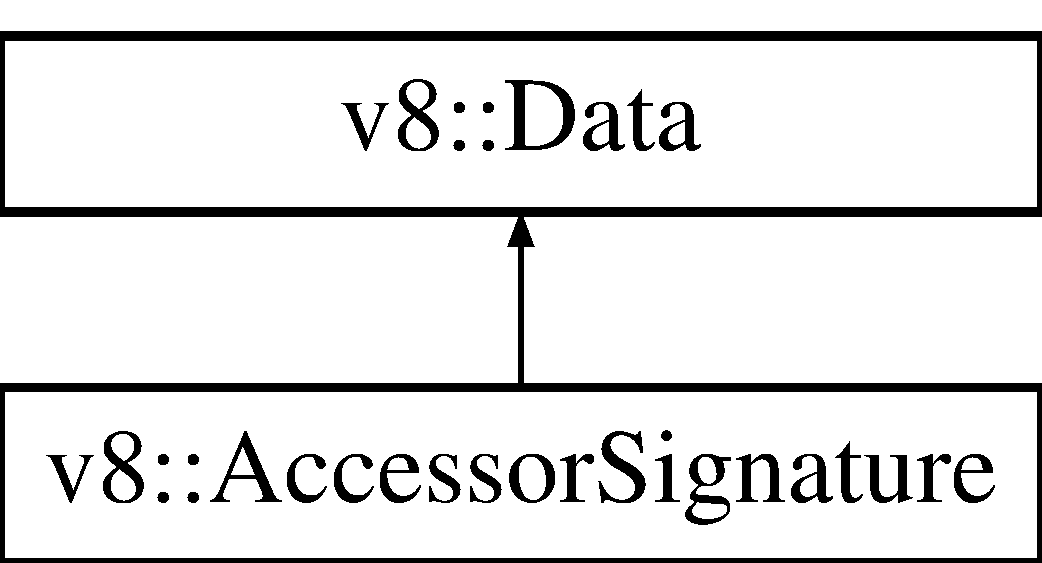
\includegraphics[height=2.000000cm]{classv8_1_1AccessorSignature}
\end{center}
\end{figure}
\subsection*{Static Public Member Functions}
\begin{DoxyCompactItemize}
\item 
\mbox{\Hypertarget{classv8_1_1AccessorSignature_a0a35126433259c49bab4d3ac6756dd67}\label{classv8_1_1AccessorSignature_a0a35126433259c49bab4d3ac6756dd67}} 
static \mbox{\hyperlink{classv8_1_1Local}{Local}}$<$ \mbox{\hyperlink{classv8_1_1AccessorSignature}{Accessor\+Signature}} $>$ {\bfseries New} (Isolate $\ast$isolate, \mbox{\hyperlink{classv8_1_1Local}{Local}}$<$ \mbox{\hyperlink{classv8_1_1FunctionTemplate}{Function\+Template}} $>$ receiver=\mbox{\hyperlink{classv8_1_1Local}{Local}}$<$ \mbox{\hyperlink{classv8_1_1FunctionTemplate}{Function\+Template}} $>$())
\item 
\mbox{\Hypertarget{classv8_1_1AccessorSignature_add2ad5697fb3b13d63de9d1e96db3758}\label{classv8_1_1AccessorSignature_add2ad5697fb3b13d63de9d1e96db3758}} 
static V8\+\_\+\+I\+N\+L\+I\+NE \mbox{\hyperlink{classv8_1_1AccessorSignature}{Accessor\+Signature}} $\ast$ {\bfseries Cast} (\mbox{\hyperlink{classv8_1_1Data}{Data}} $\ast$data)
\end{DoxyCompactItemize}


\subsection{Detailed Description}
An \mbox{\hyperlink{classv8_1_1AccessorSignature}{Accessor\+Signature}} specifies which receivers are valid parameters to an accessor callback. 

Definition at line 6243 of file v8.\+h.



The documentation for this class was generated from the following files\+:\begin{DoxyCompactItemize}
\item 
v8/include/v8.\+h\item 
v8/src/api.\+cc\end{DoxyCompactItemize}

\hypertarget{classv8_1_1ActivityControl}{\section{v8\-:\-:Activity\-Control Class Reference}
\label{classv8_1_1ActivityControl}\index{v8\-::\-Activity\-Control@{v8\-::\-Activity\-Control}}
}


{\ttfamily \#include $<$v8-\/profiler.\-h$>$}

\subsection*{Public Types}
\begin{DoxyCompactItemize}
\item 
enum {\bfseries Control\-Option} \{ {\bfseries k\-Continue} =  0, 
{\bfseries k\-Abort} =  1
 \}
\end{DoxyCompactItemize}
\subsection*{Public Member Functions}
\begin{DoxyCompactItemize}
\item 
virtual Control\-Option \hyperlink{classv8_1_1ActivityControl_a1300f10611306a3e8f79239e057eb0bf}{Report\-Progress\-Value} (int done, int total)=0
\end{DoxyCompactItemize}


\subsection{Detailed Description}
An interface for reporting progress and controlling long-\/running activities. 

\subsection{Member Function Documentation}
\hypertarget{classv8_1_1ActivityControl_a1300f10611306a3e8f79239e057eb0bf}{\index{v8\-::\-Activity\-Control@{v8\-::\-Activity\-Control}!Report\-Progress\-Value@{Report\-Progress\-Value}}
\index{Report\-Progress\-Value@{Report\-Progress\-Value}!v8::ActivityControl@{v8\-::\-Activity\-Control}}
\subsubsection[{Report\-Progress\-Value}]{\setlength{\rightskip}{0pt plus 5cm}virtual Control\-Option v8\-::\-Activity\-Control\-::\-Report\-Progress\-Value (
\begin{DoxyParamCaption}
\item[{int}]{done, }
\item[{int}]{total}
\end{DoxyParamCaption}
)\hspace{0.3cm}{\ttfamily [pure virtual]}}}\label{classv8_1_1ActivityControl_a1300f10611306a3e8f79239e057eb0bf}
Notify about current progress. The activity can be stopped by returning k\-Abort as the callback result. 

The documentation for this class was generated from the following file\-:\begin{DoxyCompactItemize}
\item 
v8/include/v8-\/profiler.\-h\end{DoxyCompactItemize}

\hypertarget{classv8_1_1AlignOfHelper}{}\section{v8\+:\+:Align\+Of\+Helper$<$ T $>$ Class Template Reference}
\label{classv8_1_1AlignOfHelper}\index{v8\+::\+Align\+Of\+Helper$<$ T $>$@{v8\+::\+Align\+Of\+Helper$<$ T $>$}}


\subsection{Detailed Description}
\subsubsection*{template$<$typename T$>$\newline
class v8\+::\+Align\+Of\+Helper$<$ T $>$}



Definition at line 414 of file v8config.\+h.



The documentation for this class was generated from the following file\+:\begin{DoxyCompactItemize}
\item 
v8/include/v8config.\+h\end{DoxyCompactItemize}

\hypertarget{classv8_1_1ArrayBuffer_1_1Allocator}{}\section{v8\+:\+:Array\+Buffer\+:\+:Allocator Class Reference}
\label{classv8_1_1ArrayBuffer_1_1Allocator}\index{v8\+::\+Array\+Buffer\+::\+Allocator@{v8\+::\+Array\+Buffer\+::\+Allocator}}


{\ttfamily \#include $<$v8.\+h$>$}

\subsection*{Public Types}
\begin{DoxyCompactItemize}
\item 
enum \mbox{\hyperlink{classv8_1_1ArrayBuffer_1_1Allocator_ab106d1fbad7be9f6fd8b0f5c550ac59e}{Allocation\+Mode}} \{ {\bfseries k\+Normal}, 
{\bfseries k\+Reservation}
 \}
\end{DoxyCompactItemize}
\subsection*{Public Member Functions}
\begin{DoxyCompactItemize}
\item 
virtual void $\ast$ \mbox{\hyperlink{classv8_1_1ArrayBuffer_1_1Allocator_a106b0d80120ed04fe9b9675e96f0340b}{Allocate}} (\mbox{\hyperlink{classsize__t}{size\+\_\+t}} length)=0
\item 
virtual void $\ast$ \mbox{\hyperlink{classv8_1_1ArrayBuffer_1_1Allocator_a92b2d5c0a826d3c435e12f3ee178f37a}{Allocate\+Uninitialized}} (\mbox{\hyperlink{classsize__t}{size\+\_\+t}} length)=0
\item 
virtual void \mbox{\hyperlink{classv8_1_1ArrayBuffer_1_1Allocator_a419f59d2a103a5a8863809d7977c9cd8}{Free}} (void $\ast$data, \mbox{\hyperlink{classsize__t}{size\+\_\+t}} length)=0
\end{DoxyCompactItemize}
\subsection*{Static Public Member Functions}
\begin{DoxyCompactItemize}
\item 
static \mbox{\hyperlink{classv8_1_1ArrayBuffer_1_1Allocator}{Allocator}} $\ast$ \mbox{\hyperlink{classv8_1_1ArrayBuffer_1_1Allocator_a2c95b1213b0a0a2996e1c63194fc6951}{New\+Default\+Allocator}} ()
\end{DoxyCompactItemize}


\subsection{Detailed Description}
A thread-\/safe allocator that V8 uses to allocate $\vert$\+Array\+Buffer$\vert$\textquotesingle{}s memory. The allocator is a global V8 setting. It has to be set via \mbox{\hyperlink{structv8_1_1Isolate_1_1CreateParams}{Isolate\+::\+Create\+Params}}.

Memory allocated through this allocator by V8 is accounted for as external memory by V8. Note that V8 keeps track of the memory for all internalized $\vert$\+Array\+Buffer$\vert$s. Responsibility for tracking external memory (using Isolate\+::\+Adjust\+Amount\+Of\+External\+Allocated\+Memory) is handed over to the embedder upon externalization and taken over upon internalization (creating an internalized buffer from an existing buffer).

Note that it is unsafe to call back into V8 from any of the allocator functions. 

Definition at line 4513 of file v8.\+h.



\subsection{Member Enumeration Documentation}
\mbox{\Hypertarget{classv8_1_1ArrayBuffer_1_1Allocator_ab106d1fbad7be9f6fd8b0f5c550ac59e}\label{classv8_1_1ArrayBuffer_1_1Allocator_ab106d1fbad7be9f6fd8b0f5c550ac59e}} 
\index{v8\+::\+Array\+Buffer\+::\+Allocator@{v8\+::\+Array\+Buffer\+::\+Allocator}!Allocation\+Mode@{Allocation\+Mode}}
\index{Allocation\+Mode@{Allocation\+Mode}!v8\+::\+Array\+Buffer\+::\+Allocator@{v8\+::\+Array\+Buffer\+::\+Allocator}}
\subsubsection{\texorpdfstring{Allocation\+Mode}{AllocationMode}}
{\footnotesize\ttfamily enum \mbox{\hyperlink{classv8_1_1ArrayBuffer_1_1Allocator_ab106d1fbad7be9f6fd8b0f5c550ac59e}{v8\+::\+Array\+Buffer\+::\+Allocator\+::\+Allocation\+Mode}}\hspace{0.3cm}{\ttfamily [strong]}}

\mbox{\hyperlink{classv8_1_1ArrayBuffer}{Array\+Buffer}} allocation mode. k\+Normal is a malloc/free style allocation, while k\+Reservation is for larger allocations with the ability to set access permissions. 

Definition at line 4540 of file v8.\+h.



\subsection{Member Function Documentation}
\mbox{\Hypertarget{classv8_1_1ArrayBuffer_1_1Allocator_a106b0d80120ed04fe9b9675e96f0340b}\label{classv8_1_1ArrayBuffer_1_1Allocator_a106b0d80120ed04fe9b9675e96f0340b}} 
\index{v8\+::\+Array\+Buffer\+::\+Allocator@{v8\+::\+Array\+Buffer\+::\+Allocator}!Allocate@{Allocate}}
\index{Allocate@{Allocate}!v8\+::\+Array\+Buffer\+::\+Allocator@{v8\+::\+Array\+Buffer\+::\+Allocator}}
\subsubsection{\texorpdfstring{Allocate()}{Allocate()}}
{\footnotesize\ttfamily virtual void$\ast$ v8\+::\+Array\+Buffer\+::\+Allocator\+::\+Allocate (\begin{DoxyParamCaption}\item[{\mbox{\hyperlink{classsize__t}{size\+\_\+t}}}]{length }\end{DoxyParamCaption})\hspace{0.3cm}{\ttfamily [pure virtual]}}

Allocate $\vert$length$\vert$ bytes. Return N\+U\+LL if allocation is not successful. Memory should be initialized to zeroes. \mbox{\Hypertarget{classv8_1_1ArrayBuffer_1_1Allocator_a92b2d5c0a826d3c435e12f3ee178f37a}\label{classv8_1_1ArrayBuffer_1_1Allocator_a92b2d5c0a826d3c435e12f3ee178f37a}} 
\index{v8\+::\+Array\+Buffer\+::\+Allocator@{v8\+::\+Array\+Buffer\+::\+Allocator}!Allocate\+Uninitialized@{Allocate\+Uninitialized}}
\index{Allocate\+Uninitialized@{Allocate\+Uninitialized}!v8\+::\+Array\+Buffer\+::\+Allocator@{v8\+::\+Array\+Buffer\+::\+Allocator}}
\subsubsection{\texorpdfstring{Allocate\+Uninitialized()}{AllocateUninitialized()}}
{\footnotesize\ttfamily virtual void$\ast$ v8\+::\+Array\+Buffer\+::\+Allocator\+::\+Allocate\+Uninitialized (\begin{DoxyParamCaption}\item[{\mbox{\hyperlink{classsize__t}{size\+\_\+t}}}]{length }\end{DoxyParamCaption})\hspace{0.3cm}{\ttfamily [pure virtual]}}

Allocate $\vert$length$\vert$ bytes. Return N\+U\+LL if allocation is not successful. Memory does not have to be initialized. \mbox{\Hypertarget{classv8_1_1ArrayBuffer_1_1Allocator_a419f59d2a103a5a8863809d7977c9cd8}\label{classv8_1_1ArrayBuffer_1_1Allocator_a419f59d2a103a5a8863809d7977c9cd8}} 
\index{v8\+::\+Array\+Buffer\+::\+Allocator@{v8\+::\+Array\+Buffer\+::\+Allocator}!Free@{Free}}
\index{Free@{Free}!v8\+::\+Array\+Buffer\+::\+Allocator@{v8\+::\+Array\+Buffer\+::\+Allocator}}
\subsubsection{\texorpdfstring{Free()}{Free()}}
{\footnotesize\ttfamily virtual void v8\+::\+Array\+Buffer\+::\+Allocator\+::\+Free (\begin{DoxyParamCaption}\item[{void $\ast$}]{data,  }\item[{\mbox{\hyperlink{classsize__t}{size\+\_\+t}}}]{length }\end{DoxyParamCaption})\hspace{0.3cm}{\ttfamily [pure virtual]}}

Free the memory block of size $\vert$length$\vert$, pointed to by $\vert$data$\vert$. That memory is guaranteed to be previously allocated by $\vert$\+Allocate$\vert$. \mbox{\Hypertarget{classv8_1_1ArrayBuffer_1_1Allocator_a2c95b1213b0a0a2996e1c63194fc6951}\label{classv8_1_1ArrayBuffer_1_1Allocator_a2c95b1213b0a0a2996e1c63194fc6951}} 
\index{v8\+::\+Array\+Buffer\+::\+Allocator@{v8\+::\+Array\+Buffer\+::\+Allocator}!New\+Default\+Allocator@{New\+Default\+Allocator}}
\index{New\+Default\+Allocator@{New\+Default\+Allocator}!v8\+::\+Array\+Buffer\+::\+Allocator@{v8\+::\+Array\+Buffer\+::\+Allocator}}
\subsubsection{\texorpdfstring{New\+Default\+Allocator()}{NewDefaultAllocator()}}
{\footnotesize\ttfamily \mbox{\hyperlink{classv8_1_1ArrayBuffer_1_1Allocator}{v8\+::\+Array\+Buffer\+::\+Allocator}} $\ast$ v8\+::\+Array\+Buffer\+::\+Allocator\+::\+New\+Default\+Allocator (\begin{DoxyParamCaption}{ }\end{DoxyParamCaption})\hspace{0.3cm}{\ttfamily [static]}}

malloc/free based convenience allocator.

Caller takes ownership, i.\+e. the returned object needs to be freed using $\vert$delete allocator$\vert$ once it is no longer in use. 

Definition at line 7543 of file api.\+cc.



The documentation for this class was generated from the following files\+:\begin{DoxyCompactItemize}
\item 
v8/include/v8.\+h\item 
v8/src/api.\+cc\end{DoxyCompactItemize}

\hypertarget{classv8_1_1Isolate_1_1AllowJavascriptExecutionScope}{}\section{v8\+:\+:Isolate\+:\+:Allow\+Javascript\+Execution\+Scope Class Reference}
\label{classv8_1_1Isolate_1_1AllowJavascriptExecutionScope}\index{v8\+::\+Isolate\+::\+Allow\+Javascript\+Execution\+Scope@{v8\+::\+Isolate\+::\+Allow\+Javascript\+Execution\+Scope}}


{\ttfamily \#include $<$v8.\+h$>$}

\subsection*{Public Member Functions}
\begin{DoxyCompactItemize}
\item 
\mbox{\Hypertarget{classv8_1_1Isolate_1_1AllowJavascriptExecutionScope_ac73a647c33756c6b7c3896170e069e8c}\label{classv8_1_1Isolate_1_1AllowJavascriptExecutionScope_ac73a647c33756c6b7c3896170e069e8c}} 
{\bfseries Allow\+Javascript\+Execution\+Scope} (Isolate $\ast$isolate)
\item 
\mbox{\Hypertarget{classv8_1_1Isolate_1_1AllowJavascriptExecutionScope_a20bf639420617b08404e2bed1b203dbc}\label{classv8_1_1Isolate_1_1AllowJavascriptExecutionScope_a20bf639420617b08404e2bed1b203dbc}} 
{\bfseries Allow\+Javascript\+Execution\+Scope} (const \mbox{\hyperlink{classv8_1_1Isolate_1_1AllowJavascriptExecutionScope}{Allow\+Javascript\+Execution\+Scope}} \&)=delete
\item 
\mbox{\Hypertarget{classv8_1_1Isolate_1_1AllowJavascriptExecutionScope_a436e3fc96e3796ccfd265a153d71224a}\label{classv8_1_1Isolate_1_1AllowJavascriptExecutionScope_a436e3fc96e3796ccfd265a153d71224a}} 
\mbox{\hyperlink{classv8_1_1Isolate_1_1AllowJavascriptExecutionScope}{Allow\+Javascript\+Execution\+Scope}} \& {\bfseries operator=} (const \mbox{\hyperlink{classv8_1_1Isolate_1_1AllowJavascriptExecutionScope}{Allow\+Javascript\+Execution\+Scope}} \&)=delete
\end{DoxyCompactItemize}


\subsection{Detailed Description}
Introduce exception to \mbox{\hyperlink{classv8_1_1Isolate_1_1DisallowJavascriptExecutionScope}{Disallow\+Javascript\+Execution\+Scope}}. 

Definition at line 7251 of file v8.\+h.



The documentation for this class was generated from the following files\+:\begin{DoxyCompactItemize}
\item 
v8/include/v8.\+h\item 
v8/src/api.\+cc\end{DoxyCompactItemize}

\hypertarget{classv8_1_1Array}{\section{v8\-:\-:Array Class Reference}
\label{classv8_1_1Array}\index{v8\-::\-Array@{v8\-::\-Array}}
}


{\ttfamily \#include $<$v8.\-h$>$}

Inheritance diagram for v8\-:\-:Array\-:\begin{figure}[H]
\begin{center}
\leavevmode
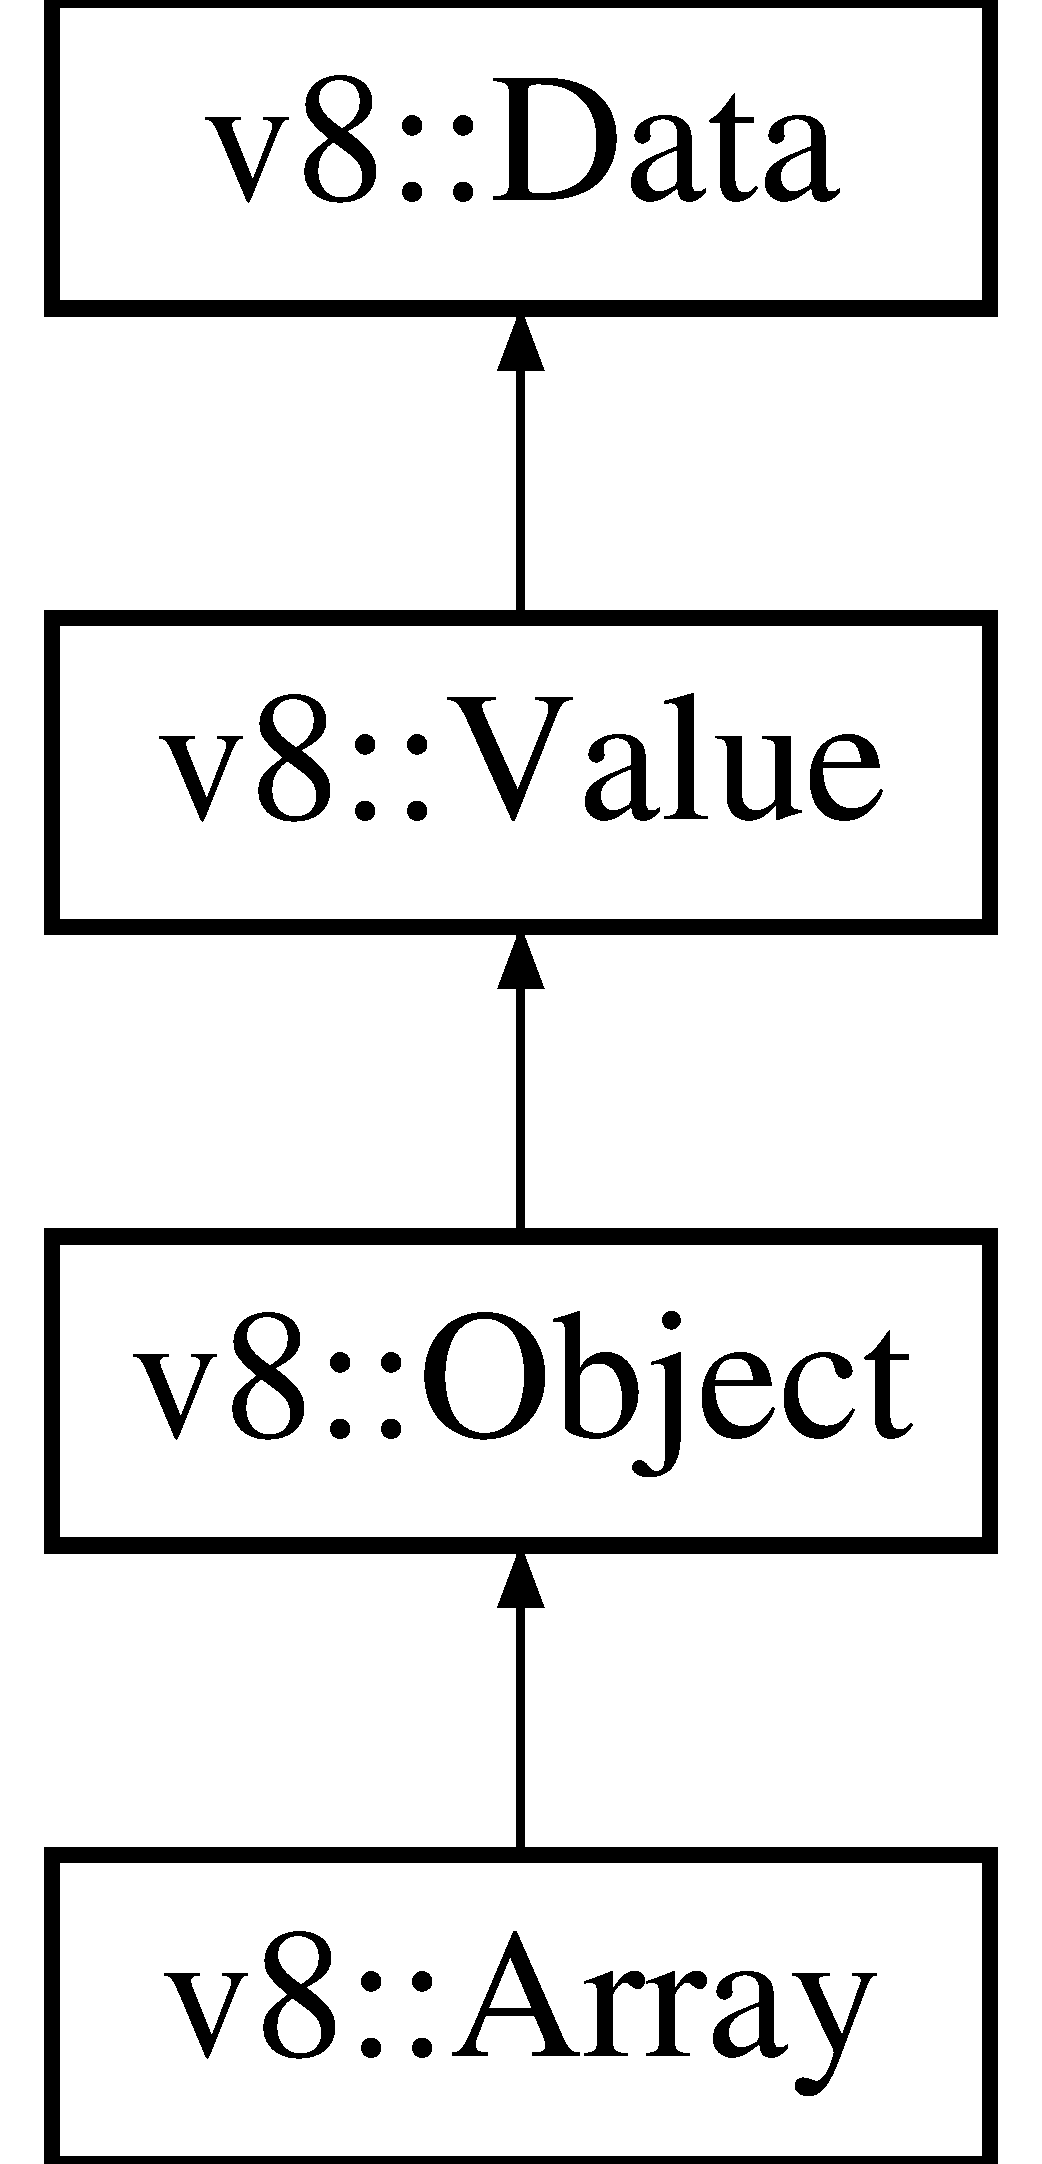
\includegraphics[height=4.000000cm]{classv8_1_1Array}
\end{center}
\end{figure}
\subsection*{Public Member Functions}
\begin{DoxyCompactItemize}
\item 
\hypertarget{classv8_1_1Array_a3c47dfd8d26e60ed4fcdc683034d6d9c}{uint32\-\_\-t {\bfseries Length} () const }\label{classv8_1_1Array_a3c47dfd8d26e60ed4fcdc683034d6d9c}

\item 
\hyperlink{classv8_1_1Local}{Local}$<$ \hyperlink{classv8_1_1Object}{Object} $>$ \hyperlink{classv8_1_1Array_a7335096a5349ce75b38d5b24af4bd125}{Clone\-Element\-At} (uint32\-\_\-t index)
\end{DoxyCompactItemize}
\subsection*{Static Public Member Functions}
\begin{DoxyCompactItemize}
\item 
static \hyperlink{classv8_1_1Local}{Local}$<$ \hyperlink{classv8_1_1Array}{Array} $>$ \hyperlink{classv8_1_1Array_a892f18fe6a25dfc0bc7b435759a30226}{New} (\hyperlink{classv8_1_1Isolate}{Isolate} $\ast$isolate, int length=0)
\item 
\hypertarget{classv8_1_1Array_ae56792766f8513395c3ebe8c29afde4b}{static V8\-\_\-\-I\-N\-L\-I\-N\-E \hyperlink{classv8_1_1Array}{Array} $\ast$ {\bfseries Cast} (\hyperlink{classv8_1_1Value}{Value} $\ast$obj)}\label{classv8_1_1Array_ae56792766f8513395c3ebe8c29afde4b}

\end{DoxyCompactItemize}


\subsection{Detailed Description}
An instance of the built-\/in array constructor (E\-C\-M\-A-\/262, 15.\-4.\-2). 

\subsection{Member Function Documentation}
\hypertarget{classv8_1_1Array_a7335096a5349ce75b38d5b24af4bd125}{\index{v8\-::\-Array@{v8\-::\-Array}!Clone\-Element\-At@{Clone\-Element\-At}}
\index{Clone\-Element\-At@{Clone\-Element\-At}!v8::Array@{v8\-::\-Array}}
\subsubsection[{Clone\-Element\-At}]{\setlength{\rightskip}{0pt plus 5cm}{\bf Local}$<${\bf Object}$>$ v8\-::\-Array\-::\-Clone\-Element\-At (
\begin{DoxyParamCaption}
\item[{uint32\-\_\-t}]{index}
\end{DoxyParamCaption}
)}}\label{classv8_1_1Array_a7335096a5349ce75b38d5b24af4bd125}
Clones an element at index $|$index$|$. Returns an empty handle if cloning fails (for any reason). \hypertarget{classv8_1_1Array_a892f18fe6a25dfc0bc7b435759a30226}{\index{v8\-::\-Array@{v8\-::\-Array}!New@{New}}
\index{New@{New}!v8::Array@{v8\-::\-Array}}
\subsubsection[{New}]{\setlength{\rightskip}{0pt plus 5cm}static {\bf Local}$<${\bf Array}$>$ v8\-::\-Array\-::\-New (
\begin{DoxyParamCaption}
\item[{{\bf Isolate} $\ast$}]{isolate, }
\item[{int}]{length = {\ttfamily 0}}
\end{DoxyParamCaption}
)\hspace{0.3cm}{\ttfamily [static]}}}\label{classv8_1_1Array_a892f18fe6a25dfc0bc7b435759a30226}
Creates a Java\-Script array with the given length. If the length is negative the returned array will have length 0. 

The documentation for this class was generated from the following file\-:\begin{DoxyCompactItemize}
\item 
v8/include/v8.\-h\end{DoxyCompactItemize}

\hypertarget{classv8_1_1ArrayBuffer}{}\section{v8\+:\+:Array\+Buffer Class Reference}
\label{classv8_1_1ArrayBuffer}\index{v8\+::\+Array\+Buffer@{v8\+::\+Array\+Buffer}}


{\ttfamily \#include $<$v8.\+h$>$}

Inheritance diagram for v8\+:\+:Array\+Buffer\+:\begin{figure}[H]
\begin{center}
\leavevmode
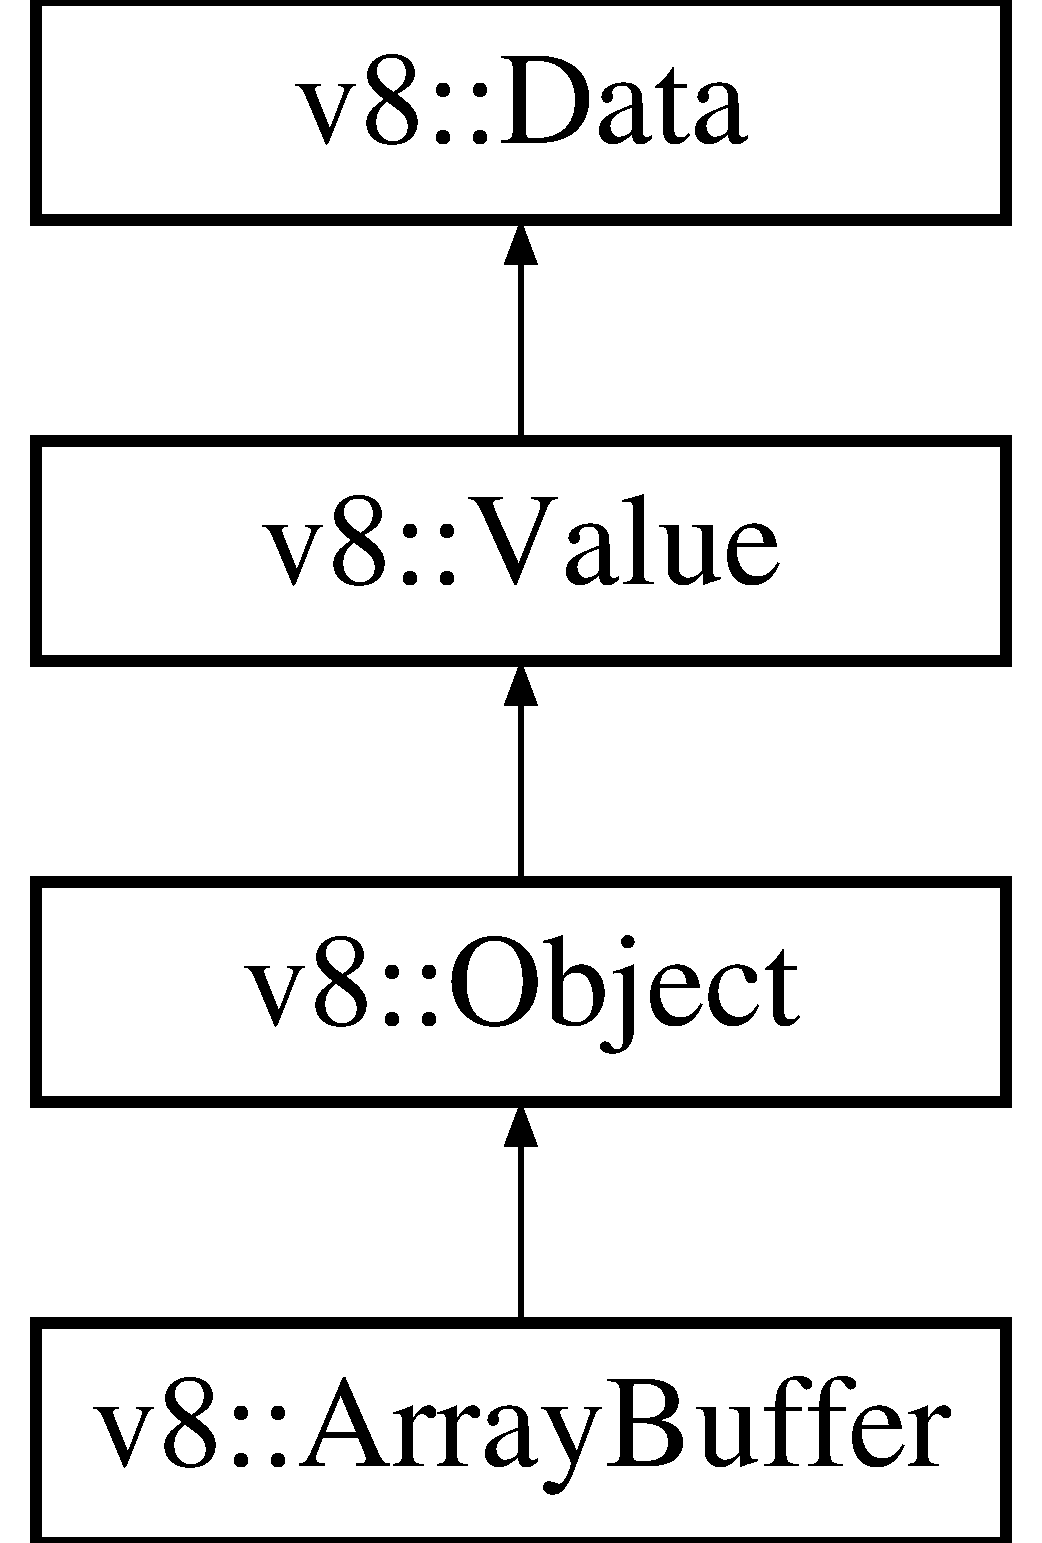
\includegraphics[height=4.000000cm]{classv8_1_1ArrayBuffer}
\end{center}
\end{figure}
\subsection*{Data Structures}
\begin{DoxyCompactItemize}
\item 
class \mbox{\hyperlink{classv8_1_1ArrayBuffer_1_1Allocator}{Allocator}}
\item 
class \mbox{\hyperlink{classv8_1_1ArrayBuffer_1_1Contents}{Contents}}
\end{DoxyCompactItemize}
\subsection*{Public Member Functions}
\begin{DoxyCompactItemize}
\item 
size\+\_\+t \mbox{\hyperlink{classv8_1_1ArrayBuffer_af4c4ad8075f74892ed3fa217219a2626}{Byte\+Length}} () const
\item 
bool \mbox{\hyperlink{classv8_1_1ArrayBuffer_a22ecea76af2257b12bdb69b40d9bec8f}{Is\+External}} () const
\item 
bool \mbox{\hyperlink{classv8_1_1ArrayBuffer_a5de3f4c29744bd89204462f987ecb626}{Is\+Neuterable}} () const
\item 
void \mbox{\hyperlink{classv8_1_1ArrayBuffer_a3420f7d38a8fe20e8f40fb82e6acb325}{Neuter}} ()
\item 
\mbox{\hyperlink{classv8_1_1ArrayBuffer_1_1Contents}{Contents}} \mbox{\hyperlink{classv8_1_1ArrayBuffer_a8b90b72486cfacb4fbec157f4803f889}{Externalize}} ()
\item 
\mbox{\hyperlink{classv8_1_1ArrayBuffer_1_1Contents}{Contents}} \mbox{\hyperlink{classv8_1_1ArrayBuffer_ae44291df12ca35de9b519e7372aa640a}{Get\+Contents}} ()
\end{DoxyCompactItemize}
\subsection*{Static Public Member Functions}
\begin{DoxyCompactItemize}
\item 
static \mbox{\hyperlink{classv8_1_1Local}{Local}}$<$ \mbox{\hyperlink{classv8_1_1ArrayBuffer}{Array\+Buffer}} $>$ \mbox{\hyperlink{classv8_1_1ArrayBuffer_ad752e03d7cc7fe863656ad6183785ab7}{New}} (Isolate $\ast$isolate, size\+\_\+t byte\+\_\+length)
\item 
static \mbox{\hyperlink{classv8_1_1Local}{Local}}$<$ \mbox{\hyperlink{classv8_1_1ArrayBuffer}{Array\+Buffer}} $>$ \mbox{\hyperlink{classv8_1_1ArrayBuffer_acc65e714766b0d0d791b0d43ec52d0bb}{New}} (Isolate $\ast$isolate, void $\ast$data, size\+\_\+t byte\+\_\+length, Array\+Buffer\+Creation\+Mode mode=Array\+Buffer\+Creation\+Mode\+::k\+Externalized)
\item 
\mbox{\Hypertarget{classv8_1_1ArrayBuffer_a4b0a703ae34217507a8ebc9cabf7336a}\label{classv8_1_1ArrayBuffer_a4b0a703ae34217507a8ebc9cabf7336a}} 
static V8\+\_\+\+I\+N\+L\+I\+NE \mbox{\hyperlink{classv8_1_1ArrayBuffer}{Array\+Buffer}} $\ast$ {\bfseries Cast} (\mbox{\hyperlink{classv8_1_1Value}{Value}} $\ast$obj)
\end{DoxyCompactItemize}
\subsection*{Static Public Attributes}
\begin{DoxyCompactItemize}
\item 
\mbox{\Hypertarget{classv8_1_1ArrayBuffer_af49000a2ea120e49da846ef02a42ac69}\label{classv8_1_1ArrayBuffer_af49000a2ea120e49da846ef02a42ac69}} 
static const int {\bfseries k\+Internal\+Field\+Count} = V8\+\_\+\+A\+R\+R\+A\+Y\+\_\+\+B\+U\+F\+F\+E\+R\+\_\+\+I\+N\+T\+E\+R\+N\+A\+L\+\_\+\+F\+I\+E\+L\+D\+\_\+\+C\+O\+U\+NT
\item 
\mbox{\Hypertarget{classv8_1_1ArrayBuffer_ae383ba945bf84433c8cd3de5d3d56345}\label{classv8_1_1ArrayBuffer_ae383ba945bf84433c8cd3de5d3d56345}} 
static const int {\bfseries k\+Embedder\+Field\+Count} = V8\+\_\+\+A\+R\+R\+A\+Y\+\_\+\+B\+U\+F\+F\+E\+R\+\_\+\+I\+N\+T\+E\+R\+N\+A\+L\+\_\+\+F\+I\+E\+L\+D\+\_\+\+C\+O\+U\+NT
\end{DoxyCompactItemize}


\subsection{Detailed Description}
An instance of the built-\/in \mbox{\hyperlink{classv8_1_1ArrayBuffer}{Array\+Buffer}} constructor (E\+S6 draft 15.\+13.\+5). 

\subsection{Member Function Documentation}
\mbox{\Hypertarget{classv8_1_1ArrayBuffer_af4c4ad8075f74892ed3fa217219a2626}\label{classv8_1_1ArrayBuffer_af4c4ad8075f74892ed3fa217219a2626}} 
\index{v8\+::\+Array\+Buffer@{v8\+::\+Array\+Buffer}!Byte\+Length@{Byte\+Length}}
\index{Byte\+Length@{Byte\+Length}!v8\+::\+Array\+Buffer@{v8\+::\+Array\+Buffer}}
\subsubsection{\texorpdfstring{Byte\+Length()}{ByteLength()}}
{\footnotesize\ttfamily size\+\_\+t v8\+::\+Array\+Buffer\+::\+Byte\+Length (\begin{DoxyParamCaption}{ }\end{DoxyParamCaption}) const}

\mbox{\hyperlink{classv8_1_1Data}{Data}} length in bytes. \mbox{\Hypertarget{classv8_1_1ArrayBuffer_a8b90b72486cfacb4fbec157f4803f889}\label{classv8_1_1ArrayBuffer_a8b90b72486cfacb4fbec157f4803f889}} 
\index{v8\+::\+Array\+Buffer@{v8\+::\+Array\+Buffer}!Externalize@{Externalize}}
\index{Externalize@{Externalize}!v8\+::\+Array\+Buffer@{v8\+::\+Array\+Buffer}}
\subsubsection{\texorpdfstring{Externalize()}{Externalize()}}
{\footnotesize\ttfamily \mbox{\hyperlink{classv8_1_1ArrayBuffer_1_1Contents}{Contents}} v8\+::\+Array\+Buffer\+::\+Externalize (\begin{DoxyParamCaption}{ }\end{DoxyParamCaption})}

Make this \mbox{\hyperlink{classv8_1_1ArrayBuffer}{Array\+Buffer}} external. The pointer to underlying memory block and byte length are returned as $\vert$\+Contents$\vert$ structure. After \mbox{\hyperlink{classv8_1_1ArrayBuffer}{Array\+Buffer}} had been externalized, it does no longer own the memory block. The caller should take steps to free memory when it is no longer needed.

The \mbox{\hyperlink{classv8_1_1Data}{Data}} pointer of \mbox{\hyperlink{classv8_1_1ArrayBuffer_1_1Contents}{Array\+Buffer\+::\+Contents}} must be freed using the provided deleter, which will call \mbox{\hyperlink{classv8_1_1ArrayBuffer_1_1Allocator_a419f59d2a103a5a8863809d7977c9cd8}{Array\+Buffer\+::\+Allocator\+::\+Free}} if the buffer was allocated with Arrary\+Buffer\+::\+Allocator\+::\+Allocate. \mbox{\Hypertarget{classv8_1_1ArrayBuffer_ae44291df12ca35de9b519e7372aa640a}\label{classv8_1_1ArrayBuffer_ae44291df12ca35de9b519e7372aa640a}} 
\index{v8\+::\+Array\+Buffer@{v8\+::\+Array\+Buffer}!Get\+Contents@{Get\+Contents}}
\index{Get\+Contents@{Get\+Contents}!v8\+::\+Array\+Buffer@{v8\+::\+Array\+Buffer}}
\subsubsection{\texorpdfstring{Get\+Contents()}{GetContents()}}
{\footnotesize\ttfamily \mbox{\hyperlink{classv8_1_1ArrayBuffer_1_1Contents}{Contents}} v8\+::\+Array\+Buffer\+::\+Get\+Contents (\begin{DoxyParamCaption}{ }\end{DoxyParamCaption})}

Get a pointer to the \mbox{\hyperlink{classv8_1_1ArrayBuffer}{Array\+Buffer}}\textquotesingle{}s underlying memory block without externalizing it. If the \mbox{\hyperlink{classv8_1_1ArrayBuffer}{Array\+Buffer}} is not externalized, this pointer will become invalid as soon as the \mbox{\hyperlink{classv8_1_1ArrayBuffer}{Array\+Buffer}} gets garbage collected.

The embedder should make sure to hold a strong reference to the \mbox{\hyperlink{classv8_1_1ArrayBuffer}{Array\+Buffer}} while accessing this pointer. \mbox{\Hypertarget{classv8_1_1ArrayBuffer_a22ecea76af2257b12bdb69b40d9bec8f}\label{classv8_1_1ArrayBuffer_a22ecea76af2257b12bdb69b40d9bec8f}} 
\index{v8\+::\+Array\+Buffer@{v8\+::\+Array\+Buffer}!Is\+External@{Is\+External}}
\index{Is\+External@{Is\+External}!v8\+::\+Array\+Buffer@{v8\+::\+Array\+Buffer}}
\subsubsection{\texorpdfstring{Is\+External()}{IsExternal()}}
{\footnotesize\ttfamily bool v8\+::\+Array\+Buffer\+::\+Is\+External (\begin{DoxyParamCaption}{ }\end{DoxyParamCaption}) const}

Returns true if \mbox{\hyperlink{classv8_1_1ArrayBuffer}{Array\+Buffer}} is externalized, that is, does not own its memory block. \mbox{\Hypertarget{classv8_1_1ArrayBuffer_a5de3f4c29744bd89204462f987ecb626}\label{classv8_1_1ArrayBuffer_a5de3f4c29744bd89204462f987ecb626}} 
\index{v8\+::\+Array\+Buffer@{v8\+::\+Array\+Buffer}!Is\+Neuterable@{Is\+Neuterable}}
\index{Is\+Neuterable@{Is\+Neuterable}!v8\+::\+Array\+Buffer@{v8\+::\+Array\+Buffer}}
\subsubsection{\texorpdfstring{Is\+Neuterable()}{IsNeuterable()}}
{\footnotesize\ttfamily bool v8\+::\+Array\+Buffer\+::\+Is\+Neuterable (\begin{DoxyParamCaption}{ }\end{DoxyParamCaption}) const}

Returns true if this \mbox{\hyperlink{classv8_1_1ArrayBuffer}{Array\+Buffer}} may be neutered. \mbox{\Hypertarget{classv8_1_1ArrayBuffer_a3420f7d38a8fe20e8f40fb82e6acb325}\label{classv8_1_1ArrayBuffer_a3420f7d38a8fe20e8f40fb82e6acb325}} 
\index{v8\+::\+Array\+Buffer@{v8\+::\+Array\+Buffer}!Neuter@{Neuter}}
\index{Neuter@{Neuter}!v8\+::\+Array\+Buffer@{v8\+::\+Array\+Buffer}}
\subsubsection{\texorpdfstring{Neuter()}{Neuter()}}
{\footnotesize\ttfamily void v8\+::\+Array\+Buffer\+::\+Neuter (\begin{DoxyParamCaption}{ }\end{DoxyParamCaption})}

Neuters this \mbox{\hyperlink{classv8_1_1ArrayBuffer}{Array\+Buffer}} and all its views (typed arrays). Neutering sets the byte length of the buffer and all typed arrays to zero, preventing Java\+Script from ever accessing underlying backing store. \mbox{\hyperlink{classv8_1_1ArrayBuffer}{Array\+Buffer}} should have been externalized and must be neuterable. \mbox{\Hypertarget{classv8_1_1ArrayBuffer_ad752e03d7cc7fe863656ad6183785ab7}\label{classv8_1_1ArrayBuffer_ad752e03d7cc7fe863656ad6183785ab7}} 
\index{v8\+::\+Array\+Buffer@{v8\+::\+Array\+Buffer}!New@{New}}
\index{New@{New}!v8\+::\+Array\+Buffer@{v8\+::\+Array\+Buffer}}
\subsubsection{\texorpdfstring{New()}{New()}\hspace{0.1cm}{\footnotesize\ttfamily [1/2]}}
{\footnotesize\ttfamily static \mbox{\hyperlink{classv8_1_1Local}{Local}}$<$\mbox{\hyperlink{classv8_1_1ArrayBuffer}{Array\+Buffer}}$>$ v8\+::\+Array\+Buffer\+::\+New (\begin{DoxyParamCaption}\item[{Isolate $\ast$}]{isolate,  }\item[{size\+\_\+t}]{byte\+\_\+length }\end{DoxyParamCaption})\hspace{0.3cm}{\ttfamily [static]}}

Create a new \mbox{\hyperlink{classv8_1_1ArrayBuffer}{Array\+Buffer}}. Allocate $\vert$byte\+\_\+length$\vert$ bytes. Allocated memory will be owned by a created \mbox{\hyperlink{classv8_1_1ArrayBuffer}{Array\+Buffer}} and will be deallocated when it is garbage-\/collected, unless the object is externalized. \mbox{\Hypertarget{classv8_1_1ArrayBuffer_acc65e714766b0d0d791b0d43ec52d0bb}\label{classv8_1_1ArrayBuffer_acc65e714766b0d0d791b0d43ec52d0bb}} 
\index{v8\+::\+Array\+Buffer@{v8\+::\+Array\+Buffer}!New@{New}}
\index{New@{New}!v8\+::\+Array\+Buffer@{v8\+::\+Array\+Buffer}}
\subsubsection{\texorpdfstring{New()}{New()}\hspace{0.1cm}{\footnotesize\ttfamily [2/2]}}
{\footnotesize\ttfamily static \mbox{\hyperlink{classv8_1_1Local}{Local}}$<$\mbox{\hyperlink{classv8_1_1ArrayBuffer}{Array\+Buffer}}$>$ v8\+::\+Array\+Buffer\+::\+New (\begin{DoxyParamCaption}\item[{Isolate $\ast$}]{isolate,  }\item[{void $\ast$}]{data,  }\item[{size\+\_\+t}]{byte\+\_\+length,  }\item[{Array\+Buffer\+Creation\+Mode}]{mode = {\ttfamily ArrayBufferCreationMode\+:\+:kExternalized} }\end{DoxyParamCaption})\hspace{0.3cm}{\ttfamily [static]}}

Create a new \mbox{\hyperlink{classv8_1_1ArrayBuffer}{Array\+Buffer}} over an existing memory block. The created array buffer is by default immediately in externalized state. In externalized state, the memory block will not be reclaimed when a created \mbox{\hyperlink{classv8_1_1ArrayBuffer}{Array\+Buffer}} is garbage-\/collected. In internalized state, the memory block will be released using $\vert$\+Allocator\+::\+Free$\vert$ once all Array\+Buffers referencing it are collected by the garbage collector. 

The documentation for this class was generated from the following file\+:\begin{DoxyCompactItemize}
\item 
v8/include/v8.\+h\end{DoxyCompactItemize}

\hypertarget{classv8_1_1ArrayBufferView}{}\section{v8\+:\+:Array\+Buffer\+View Class Reference}
\label{classv8_1_1ArrayBufferView}\index{v8\+::\+Array\+Buffer\+View@{v8\+::\+Array\+Buffer\+View}}


{\ttfamily \#include $<$v8.\+h$>$}

Inheritance diagram for v8\+:\+:Array\+Buffer\+View\+:\begin{figure}[H]
\begin{center}
\leavevmode
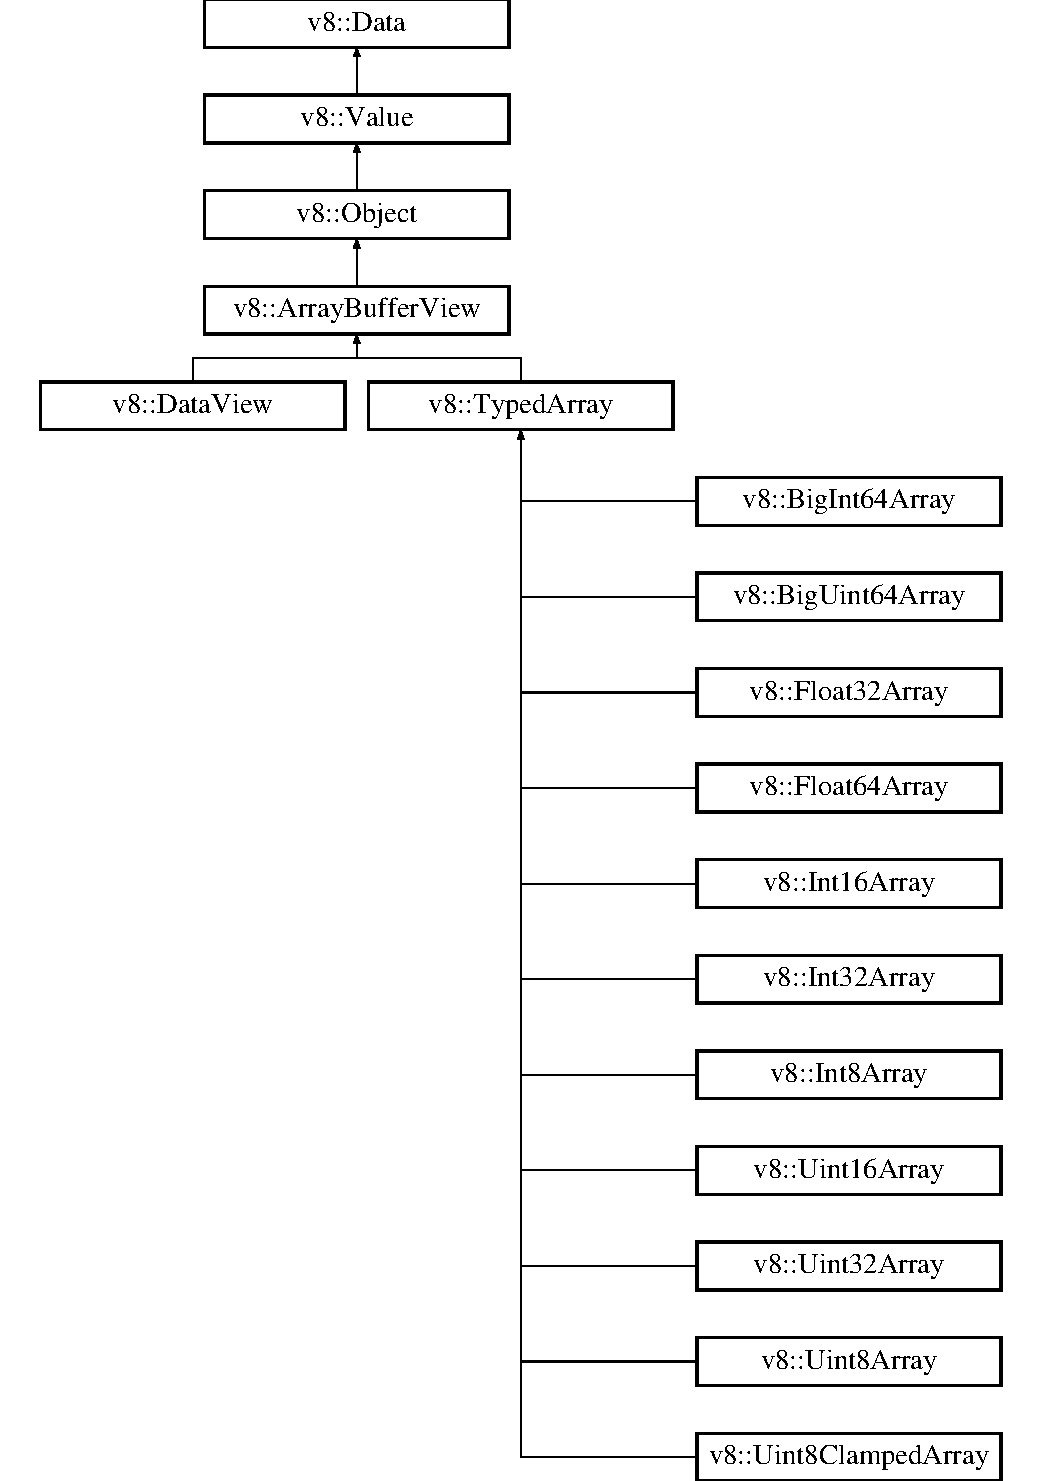
\includegraphics[height=12.000000cm]{classv8_1_1ArrayBufferView}
\end{center}
\end{figure}
\subsection*{Public Member Functions}
\begin{DoxyCompactItemize}
\item 
\mbox{\hyperlink{classv8_1_1Local}{Local}}$<$ \mbox{\hyperlink{classv8_1_1ArrayBuffer}{Array\+Buffer}} $>$ \mbox{\hyperlink{classv8_1_1ArrayBufferView_a134c62b37be7a9e8437a56b832f1800a}{Buffer}} ()
\item 
\mbox{\hyperlink{classsize__t}{size\+\_\+t}} \mbox{\hyperlink{classv8_1_1ArrayBufferView_a4739a31269f5ebc5b88a708b9429c688}{Byte\+Offset}} ()
\item 
\mbox{\hyperlink{classsize__t}{size\+\_\+t}} \mbox{\hyperlink{classv8_1_1ArrayBufferView_a9fc7563c97e0b639a6c0a3274995bb3c}{Byte\+Length}} ()
\item 
\mbox{\hyperlink{classsize__t}{size\+\_\+t}} \mbox{\hyperlink{classv8_1_1ArrayBufferView_aa728e762ed43194f3a5e05e792fff64e}{Copy\+Contents}} (void $\ast$dest, \mbox{\hyperlink{classsize__t}{size\+\_\+t}} byte\+\_\+length)
\item 
\mbox{\hyperlink{classbool}{bool}} \mbox{\hyperlink{classv8_1_1ArrayBufferView_ab1f5835c3dea53a625814a8c3ab2e0ae}{Has\+Buffer}} () const
\end{DoxyCompactItemize}
\subsection*{Static Public Member Functions}
\begin{DoxyCompactItemize}
\item 
\mbox{\Hypertarget{classv8_1_1ArrayBufferView_a84db315fe904ca1421c0e8e3f615cccb}\label{classv8_1_1ArrayBufferView_a84db315fe904ca1421c0e8e3f615cccb}} 
static V8\+\_\+\+I\+N\+L\+I\+NE \mbox{\hyperlink{classv8_1_1ArrayBufferView}{Array\+Buffer\+View}} $\ast$ {\bfseries Cast} (\mbox{\hyperlink{classv8_1_1Value}{Value}} $\ast$obj)
\end{DoxyCompactItemize}
\subsection*{Static Public Attributes}
\begin{DoxyCompactItemize}
\item 
static const \mbox{\hyperlink{classint}{int}} {\bfseries k\+Internal\+Field\+Count}
\item 
static const \mbox{\hyperlink{classint}{int}} {\bfseries k\+Embedder\+Field\+Count}
\end{DoxyCompactItemize}


\subsection{Detailed Description}
A base class for an instance of one of \char`\"{}views\char`\"{} over \mbox{\hyperlink{classv8_1_1ArrayBuffer}{Array\+Buffer}}, including Typed\+Arrays and \mbox{\hyperlink{classv8_1_1DataView}{Data\+View}} (E\+S6 draft 15.\+13). 

Definition at line 4690 of file v8.\+h.



\subsection{Member Function Documentation}
\mbox{\Hypertarget{classv8_1_1ArrayBufferView_a134c62b37be7a9e8437a56b832f1800a}\label{classv8_1_1ArrayBufferView_a134c62b37be7a9e8437a56b832f1800a}} 
\index{v8\+::\+Array\+Buffer\+View@{v8\+::\+Array\+Buffer\+View}!Buffer@{Buffer}}
\index{Buffer@{Buffer}!v8\+::\+Array\+Buffer\+View@{v8\+::\+Array\+Buffer\+View}}
\subsubsection{\texorpdfstring{Buffer()}{Buffer()}}
{\footnotesize\ttfamily \mbox{\hyperlink{classv8_1_1Local}{Local}}$<$ \mbox{\hyperlink{classv8_1_1ArrayBuffer}{Array\+Buffer}} $>$ v8\+::\+Array\+Buffer\+View\+::\+Buffer (\begin{DoxyParamCaption}{ }\end{DoxyParamCaption})}

Returns underlying \mbox{\hyperlink{classv8_1_1ArrayBuffer}{Array\+Buffer}}. 

Definition at line 7667 of file api.\+cc.

\mbox{\Hypertarget{classv8_1_1ArrayBufferView_a9fc7563c97e0b639a6c0a3274995bb3c}\label{classv8_1_1ArrayBufferView_a9fc7563c97e0b639a6c0a3274995bb3c}} 
\index{v8\+::\+Array\+Buffer\+View@{v8\+::\+Array\+Buffer\+View}!Byte\+Length@{Byte\+Length}}
\index{Byte\+Length@{Byte\+Length}!v8\+::\+Array\+Buffer\+View@{v8\+::\+Array\+Buffer\+View}}
\subsubsection{\texorpdfstring{Byte\+Length()}{ByteLength()}}
{\footnotesize\ttfamily \mbox{\hyperlink{classsize__t}{size\+\_\+t}} v8\+::\+Array\+Buffer\+View\+::\+Byte\+Length (\begin{DoxyParamCaption}{ }\end{DoxyParamCaption})}

Size of a view in bytes. 

Definition at line 7722 of file api.\+cc.

\mbox{\Hypertarget{classv8_1_1ArrayBufferView_a4739a31269f5ebc5b88a708b9429c688}\label{classv8_1_1ArrayBufferView_a4739a31269f5ebc5b88a708b9429c688}} 
\index{v8\+::\+Array\+Buffer\+View@{v8\+::\+Array\+Buffer\+View}!Byte\+Offset@{Byte\+Offset}}
\index{Byte\+Offset@{Byte\+Offset}!v8\+::\+Array\+Buffer\+View@{v8\+::\+Array\+Buffer\+View}}
\subsubsection{\texorpdfstring{Byte\+Offset()}{ByteOffset()}}
{\footnotesize\ttfamily \mbox{\hyperlink{classsize__t}{size\+\_\+t}} v8\+::\+Array\+Buffer\+View\+::\+Byte\+Offset (\begin{DoxyParamCaption}{ }\end{DoxyParamCaption})}

Byte offset in $\vert$\+Buffer$\vert$. 

Definition at line 7716 of file api.\+cc.

\mbox{\Hypertarget{classv8_1_1ArrayBufferView_aa728e762ed43194f3a5e05e792fff64e}\label{classv8_1_1ArrayBufferView_aa728e762ed43194f3a5e05e792fff64e}} 
\index{v8\+::\+Array\+Buffer\+View@{v8\+::\+Array\+Buffer\+View}!Copy\+Contents@{Copy\+Contents}}
\index{Copy\+Contents@{Copy\+Contents}!v8\+::\+Array\+Buffer\+View@{v8\+::\+Array\+Buffer\+View}}
\subsubsection{\texorpdfstring{Copy\+Contents()}{CopyContents()}}
{\footnotesize\ttfamily \mbox{\hyperlink{classsize__t}{size\+\_\+t}} v8\+::\+Array\+Buffer\+View\+::\+Copy\+Contents (\begin{DoxyParamCaption}\item[{void $\ast$}]{dest,  }\item[{\mbox{\hyperlink{classsize__t}{size\+\_\+t}}}]{byte\+\_\+length }\end{DoxyParamCaption})}

Copy the contents of the \mbox{\hyperlink{classv8_1_1ArrayBufferView}{Array\+Buffer\+View}}\textquotesingle{}s buffer to an embedder defined memory without additional overhead that calling \mbox{\hyperlink{classv8_1_1ArrayBufferView_a134c62b37be7a9e8437a56b832f1800a}{Array\+Buffer\+View\+::\+Buffer}} might incur.

Will write at most min($\vert$byte\+\_\+length$\vert$, Byte\+Length) bytes starting at Byte\+Offset of the underlying buffer to the memory starting at $\vert$dest$\vert$. Returns the number of bytes actually written. 

Definition at line 7684 of file api.\+cc.

\mbox{\Hypertarget{classv8_1_1ArrayBufferView_ab1f5835c3dea53a625814a8c3ab2e0ae}\label{classv8_1_1ArrayBufferView_ab1f5835c3dea53a625814a8c3ab2e0ae}} 
\index{v8\+::\+Array\+Buffer\+View@{v8\+::\+Array\+Buffer\+View}!Has\+Buffer@{Has\+Buffer}}
\index{Has\+Buffer@{Has\+Buffer}!v8\+::\+Array\+Buffer\+View@{v8\+::\+Array\+Buffer\+View}}
\subsubsection{\texorpdfstring{Has\+Buffer()}{HasBuffer()}}
{\footnotesize\ttfamily \mbox{\hyperlink{classbool}{bool}} v8\+::\+Array\+Buffer\+View\+::\+Has\+Buffer (\begin{DoxyParamCaption}{ }\end{DoxyParamCaption}) const}

Returns true if \mbox{\hyperlink{classv8_1_1ArrayBufferView}{Array\+Buffer\+View}}\textquotesingle{}s backing \mbox{\hyperlink{classv8_1_1ArrayBuffer}{Array\+Buffer}} has already been allocated. 

Definition at line 7708 of file api.\+cc.



\subsection{Member Data Documentation}
\mbox{\Hypertarget{classv8_1_1ArrayBufferView_a4c007c4f644125cee1b7605c9ea1bc6c}\label{classv8_1_1ArrayBufferView_a4c007c4f644125cee1b7605c9ea1bc6c}} 
\index{v8\+::\+Array\+Buffer\+View@{v8\+::\+Array\+Buffer\+View}!k\+Embedder\+Field\+Count@{k\+Embedder\+Field\+Count}}
\index{k\+Embedder\+Field\+Count@{k\+Embedder\+Field\+Count}!v8\+::\+Array\+Buffer\+View@{v8\+::\+Array\+Buffer\+View}}
\subsubsection{\texorpdfstring{k\+Embedder\+Field\+Count}{kEmbedderFieldCount}}
{\footnotesize\ttfamily const \mbox{\hyperlink{classint}{int}} v8\+::\+Array\+Buffer\+View\+::k\+Embedder\+Field\+Count\hspace{0.3cm}{\ttfamily [static]}}

{\bfseries Initial value\+:}
\begin{DoxyCode}
=
      V8\_ARRAY\_BUFFER\_VIEW\_INTERNAL\_FIELD\_COUNT
\end{DoxyCode}


Definition at line 4726 of file v8.\+h.

\mbox{\Hypertarget{classv8_1_1ArrayBufferView_a1cccb675b1a91e61411fee5918d451db}\label{classv8_1_1ArrayBufferView_a1cccb675b1a91e61411fee5918d451db}} 
\index{v8\+::\+Array\+Buffer\+View@{v8\+::\+Array\+Buffer\+View}!k\+Internal\+Field\+Count@{k\+Internal\+Field\+Count}}
\index{k\+Internal\+Field\+Count@{k\+Internal\+Field\+Count}!v8\+::\+Array\+Buffer\+View@{v8\+::\+Array\+Buffer\+View}}
\subsubsection{\texorpdfstring{k\+Internal\+Field\+Count}{kInternalFieldCount}}
{\footnotesize\ttfamily const \mbox{\hyperlink{classint}{int}} v8\+::\+Array\+Buffer\+View\+::k\+Internal\+Field\+Count\hspace{0.3cm}{\ttfamily [static]}}

{\bfseries Initial value\+:}
\begin{DoxyCode}
=
      V8\_ARRAY\_BUFFER\_VIEW\_INTERNAL\_FIELD\_COUNT
\end{DoxyCode}


Definition at line 4724 of file v8.\+h.



The documentation for this class was generated from the following files\+:\begin{DoxyCompactItemize}
\item 
v8/include/v8.\+h\item 
v8/src/api.\+cc\end{DoxyCompactItemize}

\hypertarget{classv8_1_1Boolean}{}\section{v8\+:\+:Boolean Class Reference}
\label{classv8_1_1Boolean}\index{v8\+::\+Boolean@{v8\+::\+Boolean}}


{\ttfamily \#include $<$v8.\+h$>$}

Inheritance diagram for v8\+:\+:Boolean\+:\begin{figure}[H]
\begin{center}
\leavevmode
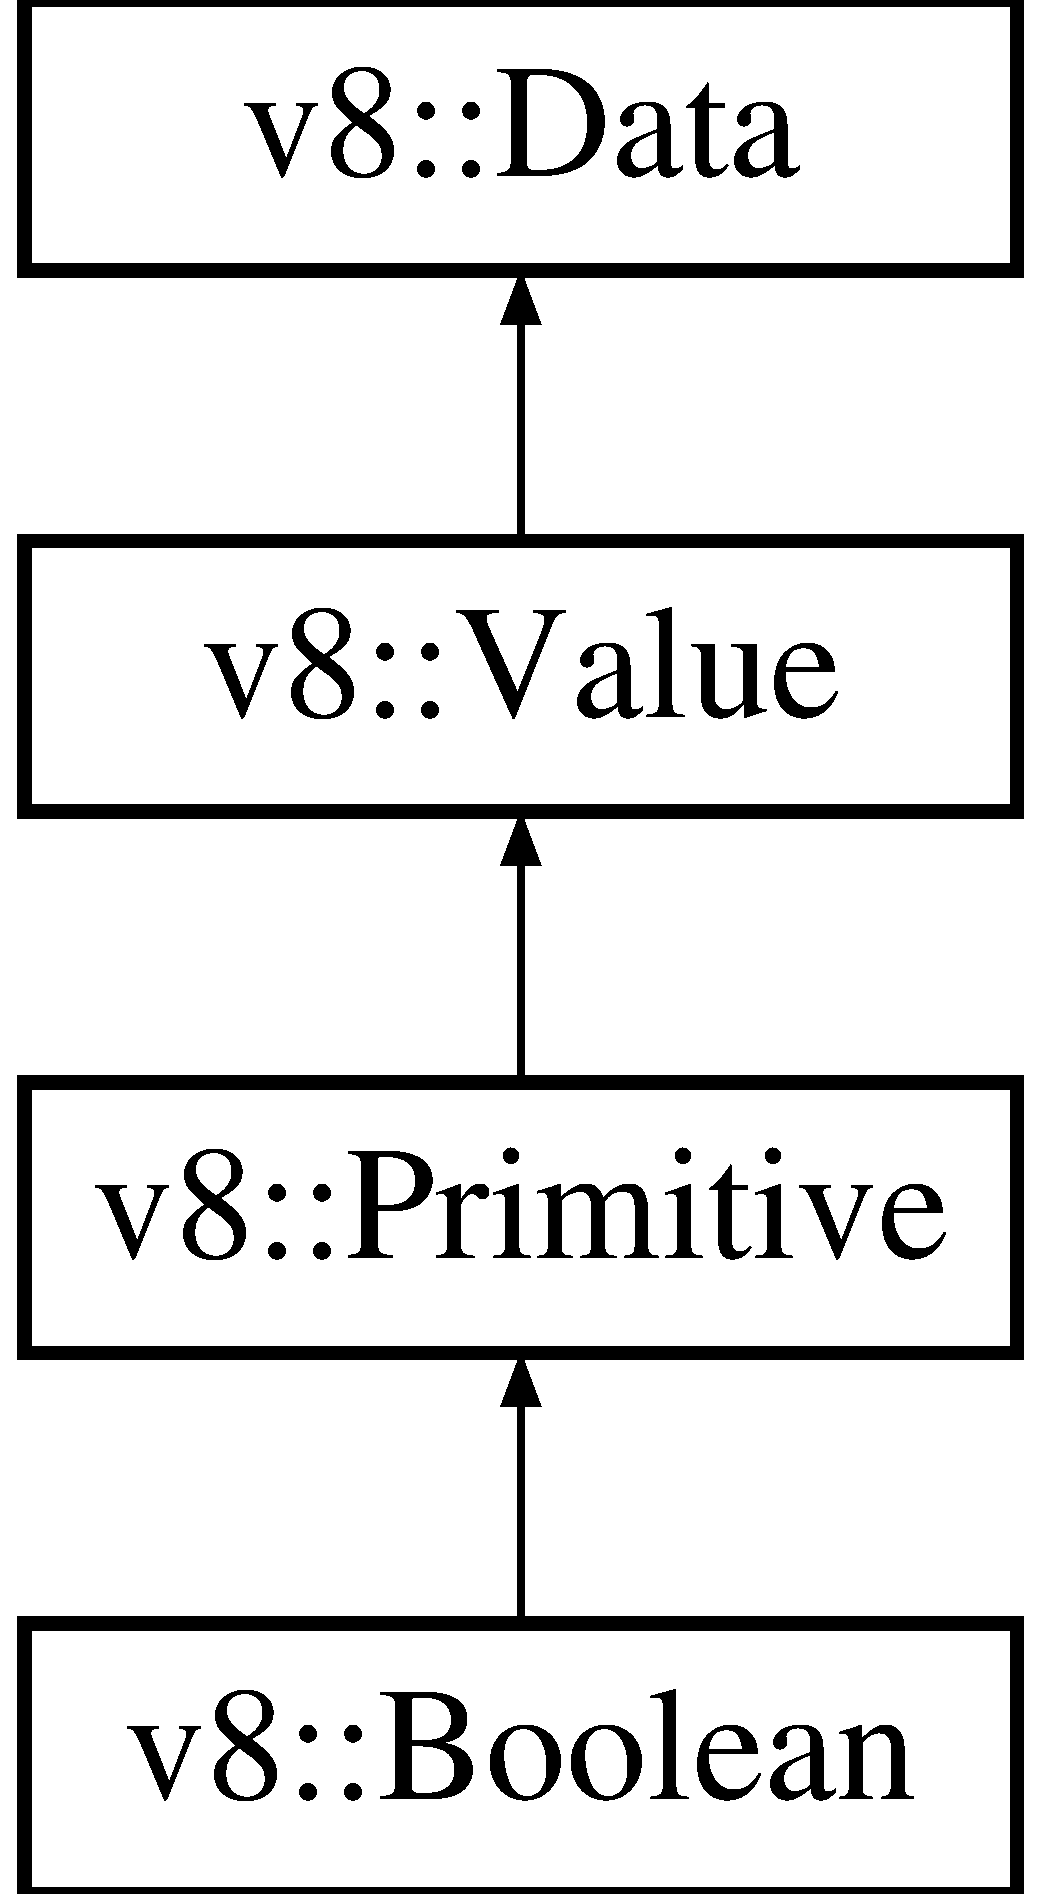
\includegraphics[height=4.000000cm]{classv8_1_1Boolean}
\end{center}
\end{figure}
\subsection*{Public Member Functions}
\begin{DoxyCompactItemize}
\item 
\hypertarget{classv8_1_1Boolean_aa493d54eb43afc64ab796e1cf66ff910}{}bool {\bfseries Value} () const \label{classv8_1_1Boolean_aa493d54eb43afc64ab796e1cf66ff910}

\end{DoxyCompactItemize}
\subsection*{Static Public Member Functions}
\begin{DoxyCompactItemize}
\item 
\hypertarget{classv8_1_1Boolean_a92493565c4b9400825a0ff09780d7ff4}{}static V8\+\_\+\+I\+N\+L\+I\+N\+E \hyperlink{classv8_1_1Boolean}{Boolean} $\ast$ {\bfseries Cast} (\hyperlink{classv8_1_1Value}{v8\+::\+Value} $\ast$obj)\label{classv8_1_1Boolean_a92493565c4b9400825a0ff09780d7ff4}

\item 
\hypertarget{classv8_1_1Boolean_aeb32aa1bf1853bc4c5f076ee6a8b9a0f}{}static V8\+\_\+\+I\+N\+L\+I\+N\+E \hyperlink{classv8_1_1Local}{Local}$<$ \hyperlink{classv8_1_1Boolean}{Boolean} $>$ {\bfseries New} (\hyperlink{classv8_1_1Isolate}{Isolate} $\ast$isolate, bool value)\label{classv8_1_1Boolean_aeb32aa1bf1853bc4c5f076ee6a8b9a0f}

\end{DoxyCompactItemize}


\subsection{Detailed Description}
A primitive boolean value (E\+C\+M\+A-\/262, 4.\+3.\+14). Either the true or false value. 

The documentation for this class was generated from the following file\+:\begin{DoxyCompactItemize}
\item 
v8/include/v8.\+h\end{DoxyCompactItemize}

\hypertarget{classv8_1_1BooleanObject}{}\section{v8\+:\+:Boolean\+Object Class Reference}
\label{classv8_1_1BooleanObject}\index{v8\+::\+Boolean\+Object@{v8\+::\+Boolean\+Object}}


{\ttfamily \#include $<$v8.\+h$>$}

Inheritance diagram for v8\+:\+:Boolean\+Object\+:\begin{figure}[H]
\begin{center}
\leavevmode
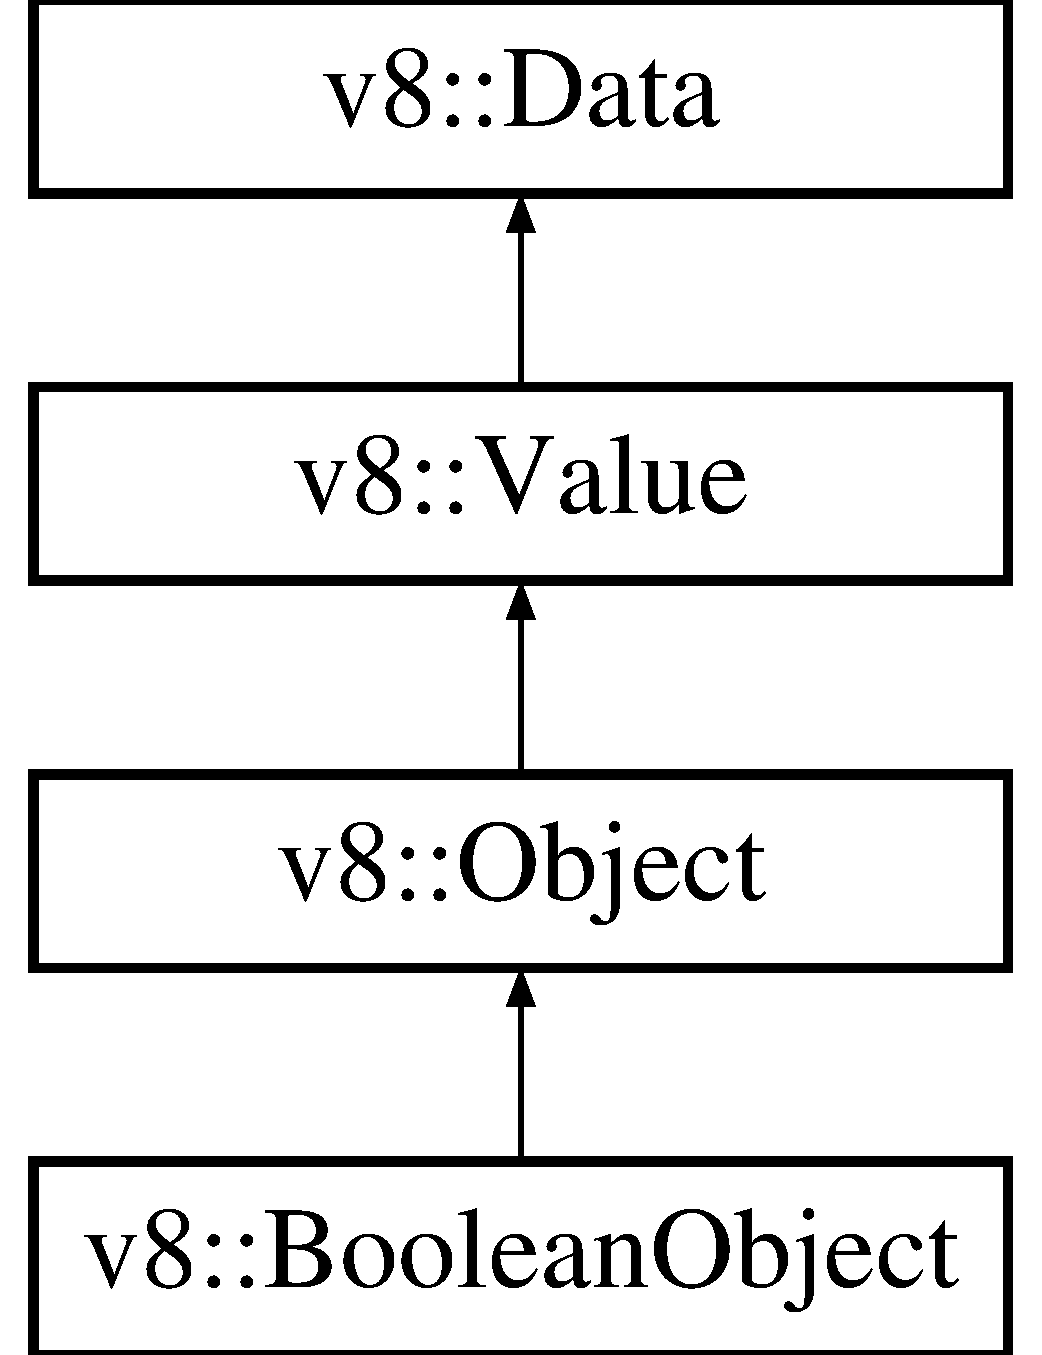
\includegraphics[height=4.000000cm]{classv8_1_1BooleanObject}
\end{center}
\end{figure}
\subsection*{Public Member Functions}
\begin{DoxyCompactItemize}
\item 
\mbox{\Hypertarget{classv8_1_1BooleanObject_a4f2f60a73ce9a730dd43046672b7b58b}\label{classv8_1_1BooleanObject_a4f2f60a73ce9a730dd43046672b7b58b}} 
bool {\bfseries Value\+Of} () const
\end{DoxyCompactItemize}
\subsection*{Static Public Member Functions}
\begin{DoxyCompactItemize}
\item 
\mbox{\Hypertarget{classv8_1_1BooleanObject_aaf29c0574a8366453ddb5a3d4f178ca4}\label{classv8_1_1BooleanObject_aaf29c0574a8366453ddb5a3d4f178ca4}} 
static \mbox{\hyperlink{classv8_1_1Local}{Local}}$<$ \mbox{\hyperlink{classv8_1_1Value}{Value}} $>$ {\bfseries New} (Isolate $\ast$isolate, bool value)
\item 
\mbox{\Hypertarget{classv8_1_1BooleanObject_a30b2a406f4dd98660c9b8f6030b3f914}\label{classv8_1_1BooleanObject_a30b2a406f4dd98660c9b8f6030b3f914}} 
static V8\+\_\+\+I\+N\+L\+I\+NE \mbox{\hyperlink{classv8_1_1BooleanObject}{Boolean\+Object}} $\ast$ {\bfseries Cast} (\mbox{\hyperlink{classv8_1_1Value}{Value}} $\ast$obj)
\end{DoxyCompactItemize}


\subsection{Detailed Description}
A \mbox{\hyperlink{classv8_1_1Boolean}{Boolean}} object (E\+C\+M\+A-\/262, 4.\+3.\+15). 

Definition at line 5157 of file v8.\+h.



The documentation for this class was generated from the following file\+:\begin{DoxyCompactItemize}
\item 
v8/include/v8.\+h\end{DoxyCompactItemize}

\hypertarget{structv8_1_1ScriptCompiler_1_1CachedData}{}\section{v8\+:\+:Script\+Compiler\+:\+:Cached\+Data Struct Reference}
\label{structv8_1_1ScriptCompiler_1_1CachedData}\index{v8\+::\+Script\+Compiler\+::\+Cached\+Data@{v8\+::\+Script\+Compiler\+::\+Cached\+Data}}


{\ttfamily \#include $<$v8.\+h$>$}

\subsection*{Public Types}
\begin{DoxyCompactItemize}
\item 
enum {\bfseries Buffer\+Policy} \{ {\bfseries Buffer\+Not\+Owned}, 
{\bfseries Buffer\+Owned}
 \}\hypertarget{structv8_1_1ScriptCompiler_1_1CachedData_ac1a1055d361e89b589c3fa98b79b9c25}{}\label{structv8_1_1ScriptCompiler_1_1CachedData_ac1a1055d361e89b589c3fa98b79b9c25}

\end{DoxyCompactItemize}
\subsection*{Public Member Functions}
\begin{DoxyCompactItemize}
\item 
{\bfseries Cached\+Data} (const uint8\+\_\+t $\ast$data, int length, Buffer\+Policy buffer\+\_\+policy=Buffer\+Not\+Owned)\hypertarget{structv8_1_1ScriptCompiler_1_1CachedData_ab45b2bd22aa86eafd0b8eecbdc72d44e}{}\label{structv8_1_1ScriptCompiler_1_1CachedData_ab45b2bd22aa86eafd0b8eecbdc72d44e}

\end{DoxyCompactItemize}
\subsection*{Data Fields}
\begin{DoxyCompactItemize}
\item 
const uint8\+\_\+t $\ast$ {\bfseries data}\hypertarget{structv8_1_1ScriptCompiler_1_1CachedData_a31e313a969170116f98d5a76c110fe61}{}\label{structv8_1_1ScriptCompiler_1_1CachedData_a31e313a969170116f98d5a76c110fe61}

\item 
int {\bfseries length}\hypertarget{structv8_1_1ScriptCompiler_1_1CachedData_ad7b8b1b672095a2c33621d3d5b5c7f8f}{}\label{structv8_1_1ScriptCompiler_1_1CachedData_ad7b8b1b672095a2c33621d3d5b5c7f8f}

\item 
bool {\bfseries rejected}\hypertarget{structv8_1_1ScriptCompiler_1_1CachedData_aa1d16fbd48957df19d4cc1c886afff8f}{}\label{structv8_1_1ScriptCompiler_1_1CachedData_aa1d16fbd48957df19d4cc1c886afff8f}

\item 
Buffer\+Policy {\bfseries buffer\+\_\+policy}\hypertarget{structv8_1_1ScriptCompiler_1_1CachedData_a1e5c9ff625ac790139aec4294493fe32}{}\label{structv8_1_1ScriptCompiler_1_1CachedData_a1e5c9ff625ac790139aec4294493fe32}

\end{DoxyCompactItemize}


\subsection{Detailed Description}
Compilation data that the embedder can cache and pass back to speed up future compilations. The data is produced if the Compiler\+Options passed to the compilation functions in \hyperlink{classv8_1_1ScriptCompiler}{Script\+Compiler} contains produce\+\_\+data\+\_\+to\+\_\+cache = true. The data to cache can then can be retrieved from \hyperlink{classv8_1_1UnboundScript}{Unbound\+Script}. 

The documentation for this struct was generated from the following file\+:\begin{DoxyCompactItemize}
\item 
v8/include/v8.\+h\end{DoxyCompactItemize}

\hypertarget{classv8_1_1Debug_1_1ClientData}{}\section{v8\+:\+:Debug\+:\+:Client\+Data Class Reference}
\label{classv8_1_1Debug_1_1ClientData}\index{v8\+::\+Debug\+::\+Client\+Data@{v8\+::\+Debug\+::\+Client\+Data}}


{\ttfamily \#include $<$v8-\/debug.\+h$>$}



\subsection{Detailed Description}
A client object passed to the \hyperlink{namespacev8}{v8} debugger whose ownership will be taken by it. \hyperlink{namespacev8}{v8} is always responsible for deleting the object. 

The documentation for this class was generated from the following file\+:\begin{DoxyCompactItemize}
\item 
v8/include/v8-\/debug.\+h\end{DoxyCompactItemize}

\hypertarget{classv8_1_1ArrayBuffer_1_1Contents}{}\section{v8\+:\+:Array\+Buffer\+:\+:Contents Class Reference}
\label{classv8_1_1ArrayBuffer_1_1Contents}\index{v8\+::\+Array\+Buffer\+::\+Contents@{v8\+::\+Array\+Buffer\+::\+Contents}}


{\ttfamily \#include $<$v8.\+h$>$}

\subsection*{Public Member Functions}
\begin{DoxyCompactItemize}
\item 
void $\ast$ {\bfseries Data} () const \hypertarget{classv8_1_1ArrayBuffer_1_1Contents_a9ed7556bfaca7a0b24deb05538a76dcd}{}\label{classv8_1_1ArrayBuffer_1_1Contents_a9ed7556bfaca7a0b24deb05538a76dcd}

\item 
size\+\_\+t {\bfseries Byte\+Length} () const \hypertarget{classv8_1_1ArrayBuffer_1_1Contents_a1b6a3eecb4fe05f4d33c83b6bc1fa737}{}\label{classv8_1_1ArrayBuffer_1_1Contents_a1b6a3eecb4fe05f4d33c83b6bc1fa737}

\end{DoxyCompactItemize}
\subsection*{Friends}
\begin{DoxyCompactItemize}
\item 
class {\bfseries Array\+Buffer}\hypertarget{classv8_1_1ArrayBuffer_1_1Contents_acbcb25033a90500a51aa19c811b2a1d3}{}\label{classv8_1_1ArrayBuffer_1_1Contents_acbcb25033a90500a51aa19c811b2a1d3}

\end{DoxyCompactItemize}


\subsection{Detailed Description}
The contents of an $\vert$\+Array\+Buffer$\vert$. Externalization of $\vert$\+Array\+Buffer$\vert$ returns an instance of this class, populated, with a pointer to data and byte length.

The \hyperlink{classv8_1_1Data}{Data} pointer of \hyperlink{classv8_1_1ArrayBuffer_1_1Contents}{Array\+Buffer\+::\+Contents} is always allocated with \hyperlink{classv8_1_1ArrayBuffer_1_1Allocator_a106b0d80120ed04fe9b9675e96f0340b}{Allocator\+::\+Allocate} that is set via \hyperlink{structv8_1_1Isolate_1_1CreateParams}{Isolate\+::\+Create\+Params}.

This A\+PI is experimental and may change significantly. 

The documentation for this class was generated from the following file\+:\begin{DoxyCompactItemize}
\item 
v8/include/v8.\+h\end{DoxyCompactItemize}

\hypertarget{classv8_1_1SharedArrayBuffer_1_1Contents}{}\section{v8\+:\+:Shared\+Array\+Buffer\+:\+:Contents Class Reference}
\label{classv8_1_1SharedArrayBuffer_1_1Contents}\index{v8\+::\+Shared\+Array\+Buffer\+::\+Contents@{v8\+::\+Shared\+Array\+Buffer\+::\+Contents}}


{\ttfamily \#include $<$v8.\+h$>$}

\subsection*{Public Member Functions}
\begin{DoxyCompactItemize}
\item 
\mbox{\Hypertarget{classv8_1_1SharedArrayBuffer_1_1Contents_a0a17b70f92830caf87f23cd3dc276489}\label{classv8_1_1SharedArrayBuffer_1_1Contents_a0a17b70f92830caf87f23cd3dc276489}} 
void $\ast$ {\bfseries Allocation\+Base} () const
\item 
\mbox{\Hypertarget{classv8_1_1SharedArrayBuffer_1_1Contents_a5d3facf7b33602f5bd8d6641c15a626a}\label{classv8_1_1SharedArrayBuffer_1_1Contents_a5d3facf7b33602f5bd8d6641c15a626a}} 
size\+\_\+t {\bfseries Allocation\+Length} () const
\item 
\mbox{\Hypertarget{classv8_1_1SharedArrayBuffer_1_1Contents_ad878fba7975a9ee251fa935c246eb4ff}\label{classv8_1_1SharedArrayBuffer_1_1Contents_ad878fba7975a9ee251fa935c246eb4ff}} 
\mbox{\hyperlink{classv8_1_1ArrayBuffer_1_1Allocator_ab106d1fbad7be9f6fd8b0f5c550ac59e}{Array\+Buffer\+::\+Allocator\+::\+Allocation\+Mode}} {\bfseries Allocation\+Mode} () const
\item 
\mbox{\Hypertarget{classv8_1_1SharedArrayBuffer_1_1Contents_a8a795e7b725530f608c83528e5d4193b}\label{classv8_1_1SharedArrayBuffer_1_1Contents_a8a795e7b725530f608c83528e5d4193b}} 
void $\ast$ {\bfseries Data} () const
\item 
\mbox{\Hypertarget{classv8_1_1SharedArrayBuffer_1_1Contents_a3678ae4afdb9884a5beeab644966382b}\label{classv8_1_1SharedArrayBuffer_1_1Contents_a3678ae4afdb9884a5beeab644966382b}} 
size\+\_\+t {\bfseries Byte\+Length} () const
\end{DoxyCompactItemize}
\subsection*{Friends}
\begin{DoxyCompactItemize}
\item 
\mbox{\Hypertarget{classv8_1_1SharedArrayBuffer_1_1Contents_a35ac2a80dda42f728b7b1dfc4c3cc040}\label{classv8_1_1SharedArrayBuffer_1_1Contents_a35ac2a80dda42f728b7b1dfc4c3cc040}} 
class {\bfseries Shared\+Array\+Buffer}
\end{DoxyCompactItemize}


\subsection{Detailed Description}
The contents of an $\vert$\+Shared\+Array\+Buffer$\vert$. Externalization of $\vert$\+Shared\+Array\+Buffer$\vert$ returns an instance of this class, populated, with a pointer to data and byte length.

The \mbox{\hyperlink{classv8_1_1Data}{Data}} pointer of \mbox{\hyperlink{classv8_1_1SharedArrayBuffer_1_1Contents}{Shared\+Array\+Buffer\+::\+Contents}} is always allocated with $\vert$\+Array\+Buffer\+::\+Allocator\+::\+Allocate$\vert$ by the allocator specified in \mbox{\hyperlink{structv8_1_1Isolate_1_1CreateParams_a7c663f70b64290392eeaf164f57585f9}{v8\+::\+Isolate\+::\+Create\+Params\+::array\+\_\+buffer\+\_\+allocator}}.

This A\+PI is experimental and may change significantly. 

The documentation for this class was generated from the following file\+:\begin{DoxyCompactItemize}
\item 
v8/include/v8.\+h\end{DoxyCompactItemize}

\hypertarget{classv8_1_1Context}{\section{v8\-:\-:Context Class Reference}
\label{classv8_1_1Context}\index{v8\-::\-Context@{v8\-::\-Context}}
}


{\ttfamily \#include $<$v8.\-h$>$}

\subsection*{Data Structures}
\begin{DoxyCompactItemize}
\item 
class \hyperlink{classv8_1_1Context_1_1Scope}{Scope}
\end{DoxyCompactItemize}
\subsection*{Public Member Functions}
\begin{DoxyCompactItemize}
\item 
\hyperlink{classv8_1_1Local}{Local}$<$ \hyperlink{classv8_1_1Object}{Object} $>$ \hyperlink{classv8_1_1Context_af5cd9f97ef6a3307c1c21f80f4b743eb}{Global} ()
\item 
void \hyperlink{classv8_1_1Context_a841c7dd92eb8c57df92a268a164dea97}{Detach\-Global} ()
\item 
void \hyperlink{classv8_1_1Context_a288d8549547f6bdf4312f5333f60f24d}{Set\-Security\-Token} (\hyperlink{classv8_1_1Handle}{Handle}$<$ \hyperlink{classv8_1_1Value}{Value} $>$ token)
\item 
void \hyperlink{classv8_1_1Context_aa9e1a14982b64fd51ab87600a287bad2}{Use\-Default\-Security\-Token} ()
\item 
\hyperlink{classv8_1_1Handle}{Handle}$<$ \hyperlink{classv8_1_1Value}{Value} $>$ \hyperlink{classv8_1_1Context_a8e71e658633518ca7718c0f6e938c6a9}{Get\-Security\-Token} ()
\item 
void \hyperlink{classv8_1_1Context_a6995c49d9897eb49053f07874b825133}{Enter} ()
\item 
void \hyperlink{classv8_1_1Context_a2db09d4fefb26023a40d88972a4c1599}{Exit} ()
\item 
\hyperlink{classv8_1_1Context_a6a4ca53837ec39c684cdbfc73ab44e4e}{V8\-\_\-\-D\-E\-P\-R\-E\-C\-A\-T\-E\-D} (\char`\"{}This can no longer happen. O\-O\-M is a fatal error.\char`\"{}, bool Has\-Out\-Of\-Memory\-Exception())
\item 
\hyperlink{classv8_1_1Isolate}{v8\-::\-Isolate} $\ast$ \hyperlink{classv8_1_1Context_af55552d8658ecb20eff7af2c83e8ede2}{Get\-Isolate} ()
\item 
V8\-\_\-\-I\-N\-L\-I\-N\-E \hyperlink{classv8_1_1Local}{Local}$<$ \hyperlink{classv8_1_1Value}{Value} $>$ \hyperlink{classv8_1_1Context_a9cfafe0ac56f6aee17eb80a913489296}{Get\-Embedder\-Data} (int index)
\item 
void \hyperlink{classv8_1_1Context_ae18e007074770872e78e0040f36de8c6}{Set\-Embedder\-Data} (int index, \hyperlink{classv8_1_1Handle}{Handle}$<$ \hyperlink{classv8_1_1Value}{Value} $>$ value)
\item 
V8\-\_\-\-I\-N\-L\-I\-N\-E void $\ast$ \hyperlink{classv8_1_1Context_aa3b5c1a1a5d145c6096840898013f559}{Get\-Aligned\-Pointer\-From\-Embedder\-Data} (int index)
\item 
void \hyperlink{classv8_1_1Context_a522063c88e4c2832f5ff4f3980815f58}{Set\-Aligned\-Pointer\-In\-Embedder\-Data} (int index, void $\ast$value)
\item 
void \hyperlink{classv8_1_1Context_a794ccc42113566f5d363f89c8b0d3c2c}{Allow\-Code\-Generation\-From\-Strings} (bool allow)
\item 
bool \hyperlink{classv8_1_1Context_aa7a960a232d232d1a2a904c2e6c18831}{Is\-Code\-Generation\-From\-Strings\-Allowed} ()
\item 
void \hyperlink{classv8_1_1Context_a6a8d067b246b8792b19e8075bc410f1d}{Set\-Error\-Message\-For\-Code\-Generation\-From\-Strings} (\hyperlink{classv8_1_1Handle}{Handle}$<$ \hyperlink{classv8_1_1String}{String} $>$ message)
\end{DoxyCompactItemize}
\subsection*{Static Public Member Functions}
\begin{DoxyCompactItemize}
\item 
static \hyperlink{classv8_1_1Local}{Local}$<$ \hyperlink{classv8_1_1Context}{Context} $>$ \hyperlink{classv8_1_1Context_a43329765465b5f525ff28368b0cef2d4}{New} (\hyperlink{classv8_1_1Isolate}{Isolate} $\ast$isolate, \hyperlink{classv8_1_1ExtensionConfiguration}{Extension\-Configuration} $\ast$extensions=N\-U\-L\-L, \hyperlink{classv8_1_1Handle}{Handle}$<$ \hyperlink{classv8_1_1ObjectTemplate}{Object\-Template} $>$ global\-\_\-template=\hyperlink{classv8_1_1Handle}{Handle}$<$ \hyperlink{classv8_1_1ObjectTemplate}{Object\-Template} $>$(), \hyperlink{classv8_1_1Handle}{Handle}$<$ \hyperlink{classv8_1_1Value}{Value} $>$ global\-\_\-object=\hyperlink{classv8_1_1Handle}{Handle}$<$ \hyperlink{classv8_1_1Value}{Value} $>$())
\end{DoxyCompactItemize}
\subsection*{Friends}
\begin{DoxyCompactItemize}
\item 
\hypertarget{classv8_1_1Context_aeceedf6e1a7d48a588516ce2b1983d6f}{class {\bfseries Value}}\label{classv8_1_1Context_aeceedf6e1a7d48a588516ce2b1983d6f}

\item 
\hypertarget{classv8_1_1Context_ae98eaa96d1b24e087f3c3e372fb09dce}{class {\bfseries Script}}\label{classv8_1_1Context_ae98eaa96d1b24e087f3c3e372fb09dce}

\item 
\hypertarget{classv8_1_1Context_a0720b5f434e636e22a3ed34f847eec57}{class {\bfseries Object}}\label{classv8_1_1Context_a0720b5f434e636e22a3ed34f847eec57}

\item 
\hypertarget{classv8_1_1Context_ab7194606aa12931e96f8f5448d418ed0}{class {\bfseries Function}}\label{classv8_1_1Context_ab7194606aa12931e96f8f5448d418ed0}

\end{DoxyCompactItemize}


\subsection{Detailed Description}
A sandboxed execution context with its own set of built-\/in objects and functions. 

\subsection{Member Function Documentation}
\hypertarget{classv8_1_1Context_a794ccc42113566f5d363f89c8b0d3c2c}{\index{v8\-::\-Context@{v8\-::\-Context}!Allow\-Code\-Generation\-From\-Strings@{Allow\-Code\-Generation\-From\-Strings}}
\index{Allow\-Code\-Generation\-From\-Strings@{Allow\-Code\-Generation\-From\-Strings}!v8::Context@{v8\-::\-Context}}
\subsubsection[{Allow\-Code\-Generation\-From\-Strings}]{\setlength{\rightskip}{0pt plus 5cm}void v8\-::\-Context\-::\-Allow\-Code\-Generation\-From\-Strings (
\begin{DoxyParamCaption}
\item[{bool}]{allow}
\end{DoxyParamCaption}
)}}\label{classv8_1_1Context_a794ccc42113566f5d363f89c8b0d3c2c}
Control whether code generation from strings is allowed. Calling this method with false will disable 'eval' and the '\hyperlink{classv8_1_1Function}{Function}' constructor for code running in this context. If 'eval' or the '\hyperlink{classv8_1_1Function}{Function}' constructor are used an exception will be thrown.

If code generation from strings is not allowed the V8\-::\-Allow\-Code\-Generation\-From\-Strings callback will be invoked if set before blocking the call to 'eval' or the '\hyperlink{classv8_1_1Function}{Function}' constructor. If that callback returns true, the call will be allowed, otherwise an exception will be thrown. If no callback is set an exception will be thrown. \hypertarget{classv8_1_1Context_a841c7dd92eb8c57df92a268a164dea97}{\index{v8\-::\-Context@{v8\-::\-Context}!Detach\-Global@{Detach\-Global}}
\index{Detach\-Global@{Detach\-Global}!v8::Context@{v8\-::\-Context}}
\subsubsection[{Detach\-Global}]{\setlength{\rightskip}{0pt plus 5cm}void v8\-::\-Context\-::\-Detach\-Global (
\begin{DoxyParamCaption}
{}
\end{DoxyParamCaption}
)}}\label{classv8_1_1Context_a841c7dd92eb8c57df92a268a164dea97}
Detaches the global object from its context before the global object can be reused to create a new context. \hypertarget{classv8_1_1Context_a6995c49d9897eb49053f07874b825133}{\index{v8\-::\-Context@{v8\-::\-Context}!Enter@{Enter}}
\index{Enter@{Enter}!v8::Context@{v8\-::\-Context}}
\subsubsection[{Enter}]{\setlength{\rightskip}{0pt plus 5cm}void v8\-::\-Context\-::\-Enter (
\begin{DoxyParamCaption}
{}
\end{DoxyParamCaption}
)}}\label{classv8_1_1Context_a6995c49d9897eb49053f07874b825133}
Enter this context. After entering a context, all code compiled and run is compiled and run in this context. If another context is already entered, this old context is saved so it can be restored when the new context is exited. \hypertarget{classv8_1_1Context_a2db09d4fefb26023a40d88972a4c1599}{\index{v8\-::\-Context@{v8\-::\-Context}!Exit@{Exit}}
\index{Exit@{Exit}!v8::Context@{v8\-::\-Context}}
\subsubsection[{Exit}]{\setlength{\rightskip}{0pt plus 5cm}void v8\-::\-Context\-::\-Exit (
\begin{DoxyParamCaption}
{}
\end{DoxyParamCaption}
)}}\label{classv8_1_1Context_a2db09d4fefb26023a40d88972a4c1599}
Exit this context. Exiting the current context restores the context that was in place when entering the current context. \hypertarget{classv8_1_1Context_aa3b5c1a1a5d145c6096840898013f559}{\index{v8\-::\-Context@{v8\-::\-Context}!Get\-Aligned\-Pointer\-From\-Embedder\-Data@{Get\-Aligned\-Pointer\-From\-Embedder\-Data}}
\index{Get\-Aligned\-Pointer\-From\-Embedder\-Data@{Get\-Aligned\-Pointer\-From\-Embedder\-Data}!v8::Context@{v8\-::\-Context}}
\subsubsection[{Get\-Aligned\-Pointer\-From\-Embedder\-Data}]{\setlength{\rightskip}{0pt plus 5cm}void $\ast$ v8\-::\-Context\-::\-Get\-Aligned\-Pointer\-From\-Embedder\-Data (
\begin{DoxyParamCaption}
\item[{int}]{index}
\end{DoxyParamCaption}
)}}\label{classv8_1_1Context_aa3b5c1a1a5d145c6096840898013f559}
Gets a 2-\/byte-\/aligned native pointer from the embedder data with the given index, which must have bees set by a previous call to Set\-Aligned\-Pointer\-In\-Embedder\-Data with the same index. Note that index 0 currently has a special meaning for Chrome's debugger. \hypertarget{classv8_1_1Context_a9cfafe0ac56f6aee17eb80a913489296}{\index{v8\-::\-Context@{v8\-::\-Context}!Get\-Embedder\-Data@{Get\-Embedder\-Data}}
\index{Get\-Embedder\-Data@{Get\-Embedder\-Data}!v8::Context@{v8\-::\-Context}}
\subsubsection[{Get\-Embedder\-Data}]{\setlength{\rightskip}{0pt plus 5cm}{\bf Local}$<$ {\bf Value} $>$ v8\-::\-Context\-::\-Get\-Embedder\-Data (
\begin{DoxyParamCaption}
\item[{int}]{index}
\end{DoxyParamCaption}
)}}\label{classv8_1_1Context_a9cfafe0ac56f6aee17eb80a913489296}
Gets the embedder data with the given index, which must have been set by a previous call to Set\-Embedder\-Data with the same index. Note that index 0 currently has a special meaning for Chrome's debugger. \hypertarget{classv8_1_1Context_af55552d8658ecb20eff7af2c83e8ede2}{\index{v8\-::\-Context@{v8\-::\-Context}!Get\-Isolate@{Get\-Isolate}}
\index{Get\-Isolate@{Get\-Isolate}!v8::Context@{v8\-::\-Context}}
\subsubsection[{Get\-Isolate}]{\setlength{\rightskip}{0pt plus 5cm}{\bf v8\-::\-Isolate}$\ast$ v8\-::\-Context\-::\-Get\-Isolate (
\begin{DoxyParamCaption}
{}
\end{DoxyParamCaption}
)}}\label{classv8_1_1Context_af55552d8658ecb20eff7af2c83e8ede2}
Returns an isolate associated with a current context. \hypertarget{classv8_1_1Context_a8e71e658633518ca7718c0f6e938c6a9}{\index{v8\-::\-Context@{v8\-::\-Context}!Get\-Security\-Token@{Get\-Security\-Token}}
\index{Get\-Security\-Token@{Get\-Security\-Token}!v8::Context@{v8\-::\-Context}}
\subsubsection[{Get\-Security\-Token}]{\setlength{\rightskip}{0pt plus 5cm}{\bf Handle}$<${\bf Value}$>$ v8\-::\-Context\-::\-Get\-Security\-Token (
\begin{DoxyParamCaption}
{}
\end{DoxyParamCaption}
)}}\label{classv8_1_1Context_a8e71e658633518ca7718c0f6e938c6a9}
Returns the security token of this context. \hypertarget{classv8_1_1Context_af5cd9f97ef6a3307c1c21f80f4b743eb}{\index{v8\-::\-Context@{v8\-::\-Context}!Global@{Global}}
\index{Global@{Global}!v8::Context@{v8\-::\-Context}}
\subsubsection[{Global}]{\setlength{\rightskip}{0pt plus 5cm}{\bf Local}$<${\bf Object}$>$ v8\-::\-Context\-::\-Global (
\begin{DoxyParamCaption}
{}
\end{DoxyParamCaption}
)}}\label{classv8_1_1Context_af5cd9f97ef6a3307c1c21f80f4b743eb}
Returns the global proxy object.

Global proxy object is a thin wrapper whose prototype points to actual context's global object with the properties like \hyperlink{classv8_1_1Object}{Object}, etc. This is done that way for security reasons (for more details see \href{https://wiki.mozilla.org/Gecko:SplitWindow}{\tt https\-://wiki.\-mozilla.\-org/\-Gecko\-:\-Split\-Window}).

Please note that changes to global proxy object prototype most probably would break V\-M---\hyperlink{namespacev8}{v8} expects only global object as a prototype of global proxy object. \hypertarget{classv8_1_1Context_aa7a960a232d232d1a2a904c2e6c18831}{\index{v8\-::\-Context@{v8\-::\-Context}!Is\-Code\-Generation\-From\-Strings\-Allowed@{Is\-Code\-Generation\-From\-Strings\-Allowed}}
\index{Is\-Code\-Generation\-From\-Strings\-Allowed@{Is\-Code\-Generation\-From\-Strings\-Allowed}!v8::Context@{v8\-::\-Context}}
\subsubsection[{Is\-Code\-Generation\-From\-Strings\-Allowed}]{\setlength{\rightskip}{0pt plus 5cm}bool v8\-::\-Context\-::\-Is\-Code\-Generation\-From\-Strings\-Allowed (
\begin{DoxyParamCaption}
{}
\end{DoxyParamCaption}
)}}\label{classv8_1_1Context_aa7a960a232d232d1a2a904c2e6c18831}
Returns true if code generation from strings is allowed for the context. For more details see \hyperlink{classv8_1_1Context_a794ccc42113566f5d363f89c8b0d3c2c}{Allow\-Code\-Generation\-From\-Strings(bool)} documentation. \hypertarget{classv8_1_1Context_a43329765465b5f525ff28368b0cef2d4}{\index{v8\-::\-Context@{v8\-::\-Context}!New@{New}}
\index{New@{New}!v8::Context@{v8\-::\-Context}}
\subsubsection[{New}]{\setlength{\rightskip}{0pt plus 5cm}static {\bf Local}$<${\bf Context}$>$ v8\-::\-Context\-::\-New (
\begin{DoxyParamCaption}
\item[{{\bf Isolate} $\ast$}]{isolate, }
\item[{{\bf Extension\-Configuration} $\ast$}]{extensions = {\ttfamily NULL}, }
\item[{{\bf Handle}$<$ {\bf Object\-Template} $>$}]{global\-\_\-template = {\ttfamily {\bf Handle}$<$~{\bf Object\-Template}~$>$()}, }
\item[{{\bf Handle}$<$ {\bf Value} $>$}]{global\-\_\-object = {\ttfamily {\bf Handle}$<$~{\bf Value}~$>$()}}
\end{DoxyParamCaption}
)\hspace{0.3cm}{\ttfamily [static]}}}\label{classv8_1_1Context_a43329765465b5f525ff28368b0cef2d4}
Creates a new context and returns a handle to the newly allocated context.


\begin{DoxyParams}{Parameters}
{\em isolate} & The isolate in which to create the context.\\
\hline
{\em extensions} & An optional extension configuration containing the extensions to be installed in the newly created context.\\
\hline
{\em global\-\_\-template} & An optional object template from which the global object for the newly created context will be created.\\
\hline
{\em global\-\_\-object} & An optional global object to be reused for the newly created context. This global object must have been created by a previous call to \hyperlink{classv8_1_1Context_a43329765465b5f525ff28368b0cef2d4}{Context\-::\-New} with the same global template. The state of the global object will be completely reset and only object identify will remain. \\
\hline
\end{DoxyParams}
\hypertarget{classv8_1_1Context_a522063c88e4c2832f5ff4f3980815f58}{\index{v8\-::\-Context@{v8\-::\-Context}!Set\-Aligned\-Pointer\-In\-Embedder\-Data@{Set\-Aligned\-Pointer\-In\-Embedder\-Data}}
\index{Set\-Aligned\-Pointer\-In\-Embedder\-Data@{Set\-Aligned\-Pointer\-In\-Embedder\-Data}!v8::Context@{v8\-::\-Context}}
\subsubsection[{Set\-Aligned\-Pointer\-In\-Embedder\-Data}]{\setlength{\rightskip}{0pt plus 5cm}void v8\-::\-Context\-::\-Set\-Aligned\-Pointer\-In\-Embedder\-Data (
\begin{DoxyParamCaption}
\item[{int}]{index, }
\item[{void $\ast$}]{value}
\end{DoxyParamCaption}
)}}\label{classv8_1_1Context_a522063c88e4c2832f5ff4f3980815f58}
Sets a 2-\/byte-\/aligned native pointer in the embedder data with the given index, growing the data as needed. Note that index 0 currently has a special meaning for Chrome's debugger. \hypertarget{classv8_1_1Context_ae18e007074770872e78e0040f36de8c6}{\index{v8\-::\-Context@{v8\-::\-Context}!Set\-Embedder\-Data@{Set\-Embedder\-Data}}
\index{Set\-Embedder\-Data@{Set\-Embedder\-Data}!v8::Context@{v8\-::\-Context}}
\subsubsection[{Set\-Embedder\-Data}]{\setlength{\rightskip}{0pt plus 5cm}void v8\-::\-Context\-::\-Set\-Embedder\-Data (
\begin{DoxyParamCaption}
\item[{int}]{index, }
\item[{{\bf Handle}$<$ {\bf Value} $>$}]{value}
\end{DoxyParamCaption}
)}}\label{classv8_1_1Context_ae18e007074770872e78e0040f36de8c6}
Sets the embedder data with the given index, growing the data as needed. Note that index 0 currently has a special meaning for Chrome's debugger. \hypertarget{classv8_1_1Context_a6a8d067b246b8792b19e8075bc410f1d}{\index{v8\-::\-Context@{v8\-::\-Context}!Set\-Error\-Message\-For\-Code\-Generation\-From\-Strings@{Set\-Error\-Message\-For\-Code\-Generation\-From\-Strings}}
\index{Set\-Error\-Message\-For\-Code\-Generation\-From\-Strings@{Set\-Error\-Message\-For\-Code\-Generation\-From\-Strings}!v8::Context@{v8\-::\-Context}}
\subsubsection[{Set\-Error\-Message\-For\-Code\-Generation\-From\-Strings}]{\setlength{\rightskip}{0pt plus 5cm}void v8\-::\-Context\-::\-Set\-Error\-Message\-For\-Code\-Generation\-From\-Strings (
\begin{DoxyParamCaption}
\item[{{\bf Handle}$<$ {\bf String} $>$}]{message}
\end{DoxyParamCaption}
)}}\label{classv8_1_1Context_a6a8d067b246b8792b19e8075bc410f1d}
Sets the error description for the exception that is thrown when code generation from strings is not allowed and 'eval' or the '\hyperlink{classv8_1_1Function}{Function}' constructor are called. \hypertarget{classv8_1_1Context_a288d8549547f6bdf4312f5333f60f24d}{\index{v8\-::\-Context@{v8\-::\-Context}!Set\-Security\-Token@{Set\-Security\-Token}}
\index{Set\-Security\-Token@{Set\-Security\-Token}!v8::Context@{v8\-::\-Context}}
\subsubsection[{Set\-Security\-Token}]{\setlength{\rightskip}{0pt plus 5cm}void v8\-::\-Context\-::\-Set\-Security\-Token (
\begin{DoxyParamCaption}
\item[{{\bf Handle}$<$ {\bf Value} $>$}]{token}
\end{DoxyParamCaption}
)}}\label{classv8_1_1Context_a288d8549547f6bdf4312f5333f60f24d}
Sets the security token for the context. To access an object in another context, the security tokens must match. \hypertarget{classv8_1_1Context_aa9e1a14982b64fd51ab87600a287bad2}{\index{v8\-::\-Context@{v8\-::\-Context}!Use\-Default\-Security\-Token@{Use\-Default\-Security\-Token}}
\index{Use\-Default\-Security\-Token@{Use\-Default\-Security\-Token}!v8::Context@{v8\-::\-Context}}
\subsubsection[{Use\-Default\-Security\-Token}]{\setlength{\rightskip}{0pt plus 5cm}void v8\-::\-Context\-::\-Use\-Default\-Security\-Token (
\begin{DoxyParamCaption}
{}
\end{DoxyParamCaption}
)}}\label{classv8_1_1Context_aa9e1a14982b64fd51ab87600a287bad2}
Restores the security token to the default value. \hypertarget{classv8_1_1Context_a6a4ca53837ec39c684cdbfc73ab44e4e}{\index{v8\-::\-Context@{v8\-::\-Context}!V8\-\_\-\-D\-E\-P\-R\-E\-C\-A\-T\-E\-D@{V8\-\_\-\-D\-E\-P\-R\-E\-C\-A\-T\-E\-D}}
\index{V8\-\_\-\-D\-E\-P\-R\-E\-C\-A\-T\-E\-D@{V8\-\_\-\-D\-E\-P\-R\-E\-C\-A\-T\-E\-D}!v8::Context@{v8\-::\-Context}}
\subsubsection[{V8\-\_\-\-D\-E\-P\-R\-E\-C\-A\-T\-E\-D}]{\setlength{\rightskip}{0pt plus 5cm}v8\-::\-Context\-::\-V8\-\_\-\-D\-E\-P\-R\-E\-C\-A\-T\-E\-D (
\begin{DoxyParamCaption}
\item[{\char`\"{}This can no longer happen. O\-O\-M is a fatal error.\char`\"{}}]{, }
\item[{bool }]{Has\-Out\-Of\-Memory\-Exception()}
\end{DoxyParamCaption}
)\hspace{0.3cm}{\ttfamily [inline]}}}\label{classv8_1_1Context_a6a4ca53837ec39c684cdbfc73ab44e4e}
Returns true if the context has experienced an out of memory situation. Since \hyperlink{classv8_1_1V8}{V8} always treats O\-O\-M as fatal error, this can no longer return true. Therefore this is now deprecated. 

The documentation for this class was generated from the following file\-:\begin{DoxyCompactItemize}
\item 
v8/include/v8.\-h\end{DoxyCompactItemize}

\hypertarget{structv8_1_1CopyablePersistentTraits}{}\section{v8\+:\+:Copyable\+Persistent\+Traits$<$ T $>$ Struct Template Reference}
\label{structv8_1_1CopyablePersistentTraits}\index{v8\+::\+Copyable\+Persistent\+Traits$<$ T $>$@{v8\+::\+Copyable\+Persistent\+Traits$<$ T $>$}}


{\ttfamily \#include $<$v8.\+h$>$}

\subsection*{Public Types}
\begin{DoxyCompactItemize}
\item 
\hypertarget{structv8_1_1CopyablePersistentTraits_a327724a22ee06da5ae54dd29982d068e}{}typedef \hyperlink{classv8_1_1Persistent}{Persistent}$<$ T, \hyperlink{structv8_1_1CopyablePersistentTraits}{Copyable\+Persistent\+Traits}$<$ T $>$ $>$ {\bfseries Copyable\+Persistent}\label{structv8_1_1CopyablePersistentTraits_a327724a22ee06da5ae54dd29982d068e}

\end{DoxyCompactItemize}
\subsection*{Static Public Member Functions}
\begin{DoxyCompactItemize}
\item 
\hypertarget{structv8_1_1CopyablePersistentTraits_aa8adf12936633b5f13b624541acaa1cf}{}{\footnotesize template$<$class S , class M $>$ }\\static V8\+\_\+\+I\+N\+L\+I\+N\+E void {\bfseries Copy} (const \hyperlink{classv8_1_1Persistent}{Persistent}$<$ S, M $>$ \&source, \hyperlink{classv8_1_1Persistent}{Copyable\+Persistent} $\ast$dest)\label{structv8_1_1CopyablePersistentTraits_aa8adf12936633b5f13b624541acaa1cf}

\end{DoxyCompactItemize}
\subsection*{Static Public Attributes}
\begin{DoxyCompactItemize}
\item 
\hypertarget{structv8_1_1CopyablePersistentTraits_a1a10842e15d8ee11f78da030bdffd025}{}static const bool {\bfseries k\+Reset\+In\+Destructor} = true\label{structv8_1_1CopyablePersistentTraits_a1a10842e15d8ee11f78da030bdffd025}

\end{DoxyCompactItemize}


\subsection{Detailed Description}
\subsubsection*{template$<$class T$>$struct v8\+::\+Copyable\+Persistent\+Traits$<$ T $>$}

Helper class traits to allow copying and assignment of \hyperlink{classv8_1_1Persistent}{Persistent}. This will clone the contents of storage cell, but not any of the flags, etc. 

The documentation for this struct was generated from the following file\+:\begin{DoxyCompactItemize}
\item 
v8/include/v8.\+h\end{DoxyCompactItemize}

\hypertarget{classv8_1_1CpuProfile}{}\section{v8\+:\+:Cpu\+Profile Class Reference}
\label{classv8_1_1CpuProfile}\index{v8\+::\+Cpu\+Profile@{v8\+::\+Cpu\+Profile}}


{\ttfamily \#include $<$v8-\/profiler.\+h$>$}

\subsection*{Public Member Functions}
\begin{DoxyCompactItemize}
\item 
\hyperlink{classv8_1_1Local}{Local}$<$ \hyperlink{classv8_1_1String}{String} $>$ \hyperlink{classv8_1_1CpuProfile_a34cc58f44862c27ea781ce47ca79f74e}{Get\+Title} () const 
\item 
const \hyperlink{classv8_1_1CpuProfileNode}{Cpu\+Profile\+Node} $\ast$ \hyperlink{classv8_1_1CpuProfile_aec978f073af6634b6495baa65209a31f}{Get\+Top\+Down\+Root} () const 
\item 
int \hyperlink{classv8_1_1CpuProfile_a2ca9d8e862dc2b06892196b5e5a14994}{Get\+Samples\+Count} () const 
\item 
const \hyperlink{classv8_1_1CpuProfileNode}{Cpu\+Profile\+Node} $\ast$ \hyperlink{classv8_1_1CpuProfile_a59470cd1286e949dd069eea87777a074}{Get\+Sample} (int index) const 
\item 
int64\+\_\+t \hyperlink{classv8_1_1CpuProfile_a310b49cf2ac856821b5db5dd856580e7}{Get\+Sample\+Timestamp} (int index) const 
\item 
int64\+\_\+t \hyperlink{classv8_1_1CpuProfile_aac317de54bdfc4523b5ecea522c01ad1}{Get\+Start\+Time} () const 
\item 
int64\+\_\+t \hyperlink{classv8_1_1CpuProfile_a15170e2e9eeb972fddf949bd08dd09ff}{Get\+End\+Time} () const 
\item 
void \hyperlink{classv8_1_1CpuProfile_a70c93f0c14d07a7e1bad42ee95665ca0}{Delete} ()
\end{DoxyCompactItemize}


\subsection{Detailed Description}
\hyperlink{classv8_1_1CpuProfile}{Cpu\+Profile} contains a C\+P\+U profile in a form of top-\/down call tree (from main() down to functions that do all the work). 

\subsection{Member Function Documentation}
\hypertarget{classv8_1_1CpuProfile_a70c93f0c14d07a7e1bad42ee95665ca0}{}\index{v8\+::\+Cpu\+Profile@{v8\+::\+Cpu\+Profile}!Delete@{Delete}}
\index{Delete@{Delete}!v8\+::\+Cpu\+Profile@{v8\+::\+Cpu\+Profile}}
\subsubsection[{Delete}]{\setlength{\rightskip}{0pt plus 5cm}void v8\+::\+Cpu\+Profile\+::\+Delete (
\begin{DoxyParamCaption}
{}
\end{DoxyParamCaption}
)}\label{classv8_1_1CpuProfile_a70c93f0c14d07a7e1bad42ee95665ca0}
Deletes the profile and removes it from \hyperlink{classv8_1_1CpuProfiler}{Cpu\+Profiler}\textquotesingle{}s list. All pointers to nodes previously returned become invalid. \hypertarget{classv8_1_1CpuProfile_a15170e2e9eeb972fddf949bd08dd09ff}{}\index{v8\+::\+Cpu\+Profile@{v8\+::\+Cpu\+Profile}!Get\+End\+Time@{Get\+End\+Time}}
\index{Get\+End\+Time@{Get\+End\+Time}!v8\+::\+Cpu\+Profile@{v8\+::\+Cpu\+Profile}}
\subsubsection[{Get\+End\+Time}]{\setlength{\rightskip}{0pt plus 5cm}int64\+\_\+t v8\+::\+Cpu\+Profile\+::\+Get\+End\+Time (
\begin{DoxyParamCaption}
{}
\end{DoxyParamCaption}
) const}\label{classv8_1_1CpuProfile_a15170e2e9eeb972fddf949bd08dd09ff}
Returns time when the profile recording was stopped (in microseconds) since some unspecified starting point. The point is equal to the starting point used by Get\+Start\+Time. \hypertarget{classv8_1_1CpuProfile_a59470cd1286e949dd069eea87777a074}{}\index{v8\+::\+Cpu\+Profile@{v8\+::\+Cpu\+Profile}!Get\+Sample@{Get\+Sample}}
\index{Get\+Sample@{Get\+Sample}!v8\+::\+Cpu\+Profile@{v8\+::\+Cpu\+Profile}}
\subsubsection[{Get\+Sample}]{\setlength{\rightskip}{0pt plus 5cm}const {\bf Cpu\+Profile\+Node}$\ast$ v8\+::\+Cpu\+Profile\+::\+Get\+Sample (
\begin{DoxyParamCaption}
\item[{int}]{index}
\end{DoxyParamCaption}
) const}\label{classv8_1_1CpuProfile_a59470cd1286e949dd069eea87777a074}
Returns profile node corresponding to the top frame the sample at the given index. \hypertarget{classv8_1_1CpuProfile_a2ca9d8e862dc2b06892196b5e5a14994}{}\index{v8\+::\+Cpu\+Profile@{v8\+::\+Cpu\+Profile}!Get\+Samples\+Count@{Get\+Samples\+Count}}
\index{Get\+Samples\+Count@{Get\+Samples\+Count}!v8\+::\+Cpu\+Profile@{v8\+::\+Cpu\+Profile}}
\subsubsection[{Get\+Samples\+Count}]{\setlength{\rightskip}{0pt plus 5cm}int v8\+::\+Cpu\+Profile\+::\+Get\+Samples\+Count (
\begin{DoxyParamCaption}
{}
\end{DoxyParamCaption}
) const}\label{classv8_1_1CpuProfile_a2ca9d8e862dc2b06892196b5e5a14994}
Returns number of samples recorded. The samples are not recorded unless $\vert$record\+\_\+samples$\vert$ parameter of Cpu\+Profiler\+::\+Start\+Cpu\+Profiling is true. \hypertarget{classv8_1_1CpuProfile_a310b49cf2ac856821b5db5dd856580e7}{}\index{v8\+::\+Cpu\+Profile@{v8\+::\+Cpu\+Profile}!Get\+Sample\+Timestamp@{Get\+Sample\+Timestamp}}
\index{Get\+Sample\+Timestamp@{Get\+Sample\+Timestamp}!v8\+::\+Cpu\+Profile@{v8\+::\+Cpu\+Profile}}
\subsubsection[{Get\+Sample\+Timestamp}]{\setlength{\rightskip}{0pt plus 5cm}int64\+\_\+t v8\+::\+Cpu\+Profile\+::\+Get\+Sample\+Timestamp (
\begin{DoxyParamCaption}
\item[{int}]{index}
\end{DoxyParamCaption}
) const}\label{classv8_1_1CpuProfile_a310b49cf2ac856821b5db5dd856580e7}
Returns the timestamp of the sample. The timestamp is the number of microseconds since some unspecified starting point. The point is equal to the starting point used by Get\+Start\+Time. \hypertarget{classv8_1_1CpuProfile_aac317de54bdfc4523b5ecea522c01ad1}{}\index{v8\+::\+Cpu\+Profile@{v8\+::\+Cpu\+Profile}!Get\+Start\+Time@{Get\+Start\+Time}}
\index{Get\+Start\+Time@{Get\+Start\+Time}!v8\+::\+Cpu\+Profile@{v8\+::\+Cpu\+Profile}}
\subsubsection[{Get\+Start\+Time}]{\setlength{\rightskip}{0pt plus 5cm}int64\+\_\+t v8\+::\+Cpu\+Profile\+::\+Get\+Start\+Time (
\begin{DoxyParamCaption}
{}
\end{DoxyParamCaption}
) const}\label{classv8_1_1CpuProfile_aac317de54bdfc4523b5ecea522c01ad1}
Returns time when the profile recording was started (in microseconds) since some unspecified starting point. \hypertarget{classv8_1_1CpuProfile_a34cc58f44862c27ea781ce47ca79f74e}{}\index{v8\+::\+Cpu\+Profile@{v8\+::\+Cpu\+Profile}!Get\+Title@{Get\+Title}}
\index{Get\+Title@{Get\+Title}!v8\+::\+Cpu\+Profile@{v8\+::\+Cpu\+Profile}}
\subsubsection[{Get\+Title}]{\setlength{\rightskip}{0pt plus 5cm}{\bf Local}$<${\bf String}$>$ v8\+::\+Cpu\+Profile\+::\+Get\+Title (
\begin{DoxyParamCaption}
{}
\end{DoxyParamCaption}
) const}\label{classv8_1_1CpuProfile_a34cc58f44862c27ea781ce47ca79f74e}
Returns C\+P\+U profile title. \hypertarget{classv8_1_1CpuProfile_aec978f073af6634b6495baa65209a31f}{}\index{v8\+::\+Cpu\+Profile@{v8\+::\+Cpu\+Profile}!Get\+Top\+Down\+Root@{Get\+Top\+Down\+Root}}
\index{Get\+Top\+Down\+Root@{Get\+Top\+Down\+Root}!v8\+::\+Cpu\+Profile@{v8\+::\+Cpu\+Profile}}
\subsubsection[{Get\+Top\+Down\+Root}]{\setlength{\rightskip}{0pt plus 5cm}const {\bf Cpu\+Profile\+Node}$\ast$ v8\+::\+Cpu\+Profile\+::\+Get\+Top\+Down\+Root (
\begin{DoxyParamCaption}
{}
\end{DoxyParamCaption}
) const}\label{classv8_1_1CpuProfile_aec978f073af6634b6495baa65209a31f}
Returns the root node of the top down call tree. 

The documentation for this class was generated from the following file\+:\begin{DoxyCompactItemize}
\item 
v8/include/v8-\/profiler.\+h\end{DoxyCompactItemize}

\hypertarget{structv8_1_1CpuProfileDeoptFrame}{}\section{v8\+:\+:Cpu\+Profile\+Deopt\+Frame Struct Reference}
\label{structv8_1_1CpuProfileDeoptFrame}\index{v8\+::\+Cpu\+Profile\+Deopt\+Frame@{v8\+::\+Cpu\+Profile\+Deopt\+Frame}}
\subsection*{Data Fields}
\begin{DoxyCompactItemize}
\item 
\mbox{\Hypertarget{structv8_1_1CpuProfileDeoptFrame_af7b750288458a70a81b4c05869b8f6d7}\label{structv8_1_1CpuProfileDeoptFrame_af7b750288458a70a81b4c05869b8f6d7}} 
int {\bfseries script\+\_\+id}
\item 
\mbox{\Hypertarget{structv8_1_1CpuProfileDeoptFrame_a4f82d1517fd15573bb2890961496a76f}\label{structv8_1_1CpuProfileDeoptFrame_a4f82d1517fd15573bb2890961496a76f}} 
size\+\_\+t {\bfseries position}
\end{DoxyCompactItemize}


The documentation for this struct was generated from the following file\+:\begin{DoxyCompactItemize}
\item 
v8/include/v8-\/profiler.\+h\end{DoxyCompactItemize}

\hypertarget{structv8_1_1CpuProfileDeoptInfo}{}\section{v8\+:\+:Cpu\+Profile\+Deopt\+Info Struct Reference}
\label{structv8_1_1CpuProfileDeoptInfo}\index{v8\+::\+Cpu\+Profile\+Deopt\+Info@{v8\+::\+Cpu\+Profile\+Deopt\+Info}}
\subsection*{Public Attributes}
\begin{DoxyCompactItemize}
\item 
const char $\ast$ \mbox{\hyperlink{structv8_1_1CpuProfileDeoptInfo_a908eb3ba33b47ace8973eeb2fda96ca9}{deopt\+\_\+reason}}
\item 
\mbox{\Hypertarget{structv8_1_1CpuProfileDeoptInfo_a9446493c0e0a00e3ada02ba8df858d42}\label{structv8_1_1CpuProfileDeoptInfo_a9446493c0e0a00e3ada02ba8df858d42}} 
std\+::vector$<$ \mbox{\hyperlink{structv8_1_1CpuProfileDeoptFrame}{Cpu\+Profile\+Deopt\+Frame}} $>$ {\bfseries stack}
\end{DoxyCompactItemize}


\subsection{Detailed Description}


Definition at line 36 of file v8-\/profiler.\+h.



\subsection{Member Data Documentation}
\mbox{\Hypertarget{structv8_1_1CpuProfileDeoptInfo_a908eb3ba33b47ace8973eeb2fda96ca9}\label{structv8_1_1CpuProfileDeoptInfo_a908eb3ba33b47ace8973eeb2fda96ca9}} 
\index{v8\+::\+Cpu\+Profile\+Deopt\+Info@{v8\+::\+Cpu\+Profile\+Deopt\+Info}!deopt\+\_\+reason@{deopt\+\_\+reason}}
\index{deopt\+\_\+reason@{deopt\+\_\+reason}!v8\+::\+Cpu\+Profile\+Deopt\+Info@{v8\+::\+Cpu\+Profile\+Deopt\+Info}}
\subsubsection{\texorpdfstring{deopt\+\_\+reason}{deopt\_reason}}
{\footnotesize\ttfamily const char$\ast$ v8\+::\+Cpu\+Profile\+Deopt\+Info\+::deopt\+\_\+reason}

A pointer to a static string owned by \mbox{\hyperlink{namespacev8}{v8}}. 

Definition at line 38 of file v8-\/profiler.\+h.



The documentation for this struct was generated from the following file\+:\begin{DoxyCompactItemize}
\item 
v8/include/v8-\/profiler.\+h\end{DoxyCompactItemize}

\hypertarget{classv8_1_1CpuProfileNode}{}\section{v8\+:\+:Cpu\+Profile\+Node Class Reference}
\label{classv8_1_1CpuProfileNode}\index{v8\+::\+Cpu\+Profile\+Node@{v8\+::\+Cpu\+Profile\+Node}}


{\ttfamily \#include $<$v8-\/profiler.\+h$>$}

\subsection*{Data Structures}
\begin{DoxyCompactItemize}
\item 
struct \hyperlink{structv8_1_1CpuProfileNode_1_1LineTick}{Line\+Tick}
\end{DoxyCompactItemize}
\subsection*{Public Member Functions}
\begin{DoxyCompactItemize}
\item 
\hyperlink{classv8_1_1Local}{Local}$<$ \hyperlink{classv8_1_1String}{String} $>$ \hyperlink{classv8_1_1CpuProfileNode_ab93a8d88fbb77a6136af4aeda92fd622}{Get\+Function\+Name} () const 
\item 
int \hyperlink{classv8_1_1CpuProfileNode_acf6f384df08ec40ff306d3e229f77258}{Get\+Script\+Id} () const 
\item 
\hyperlink{classv8_1_1Local}{Local}$<$ \hyperlink{classv8_1_1String}{String} $>$ \hyperlink{classv8_1_1CpuProfileNode_a1f27527b39f1ed83f47f4cfd58b02950}{Get\+Script\+Resource\+Name} () const 
\item 
int \hyperlink{classv8_1_1CpuProfileNode_a45ea035661c7152e4f3eb47f73787a75}{Get\+Line\+Number} () const 
\item 
int \hyperlink{classv8_1_1CpuProfileNode_a43cf237ea6f254a61a6e2a81d554aa1a}{Get\+Column\+Number} () const 
\item 
unsigned int \hyperlink{classv8_1_1CpuProfileNode_ac0d6015d3859e29db07f6a7e574426d3}{Get\+Hit\+Line\+Count} () const 
\item 
bool \hyperlink{classv8_1_1CpuProfileNode_af31611e24f47519e82b52b49969ed0a4}{Get\+Line\+Ticks} (\hyperlink{structv8_1_1CpuProfileNode_1_1LineTick}{Line\+Tick} $\ast$entries, unsigned int length) const 
\item 
const char $\ast$ \hyperlink{classv8_1_1CpuProfileNode_a16cd3d8d7ef307784838a35022507031}{Get\+Bailout\+Reason} () const 
\item 
unsigned \hyperlink{classv8_1_1CpuProfileNode_a8d297f185b0bbd9f6853f6ed193b656e}{Get\+Hit\+Count} () const 
\item 
unsigned \hyperlink{classv8_1_1CpuProfileNode_a245092eb223b948fc9441664d9e2701e}{Get\+Call\+Uid} () const 
\item 
unsigned \hyperlink{classv8_1_1CpuProfileNode_ae2971c5003353a984ef72b6cddf5e298}{Get\+Node\+Id} () const 
\item 
int \hyperlink{classv8_1_1CpuProfileNode_ac4612b91e43a2901ac20c3705288955b}{Get\+Children\+Count} () const 
\item 
const \hyperlink{classv8_1_1CpuProfileNode}{Cpu\+Profile\+Node} $\ast$ \hyperlink{classv8_1_1CpuProfileNode_aa397db1e0f5147155164c5ea3e854d69}{Get\+Child} (int index) const 
\item 
const std\+::vector$<$ \hyperlink{structv8_1_1CpuProfileDeoptInfo}{Cpu\+Profile\+Deopt\+Info} $>$ \& \hyperlink{classv8_1_1CpuProfileNode_aaca90265c1dd6dc0ba39c3d0af24ae5c}{Get\+Deopt\+Infos} () const 
\end{DoxyCompactItemize}
\subsection*{Static Public Attributes}
\begin{DoxyCompactItemize}
\item 
static const int {\bfseries k\+No\+Line\+Number\+Info} = Message\+::k\+No\+Line\+Number\+Info\hypertarget{classv8_1_1CpuProfileNode_ad54213fe8a795cb6669566f0272fc5ba}{}\label{classv8_1_1CpuProfileNode_ad54213fe8a795cb6669566f0272fc5ba}

\item 
static const int {\bfseries k\+No\+Column\+Number\+Info} = Message\+::k\+No\+Column\+Info\hypertarget{classv8_1_1CpuProfileNode_a7c8c1dea3ae0cf4c219b7b1f15a8405b}{}\label{classv8_1_1CpuProfileNode_a7c8c1dea3ae0cf4c219b7b1f15a8405b}

\end{DoxyCompactItemize}


\subsection{Detailed Description}
\hyperlink{classv8_1_1CpuProfileNode}{Cpu\+Profile\+Node} represents a node in a call graph. 

\subsection{Member Function Documentation}
\index{v8\+::\+Cpu\+Profile\+Node@{v8\+::\+Cpu\+Profile\+Node}!Get\+Bailout\+Reason@{Get\+Bailout\+Reason}}
\index{Get\+Bailout\+Reason@{Get\+Bailout\+Reason}!v8\+::\+Cpu\+Profile\+Node@{v8\+::\+Cpu\+Profile\+Node}}
\subsubsection[{\texorpdfstring{Get\+Bailout\+Reason() const }{GetBailoutReason() const }}]{\setlength{\rightskip}{0pt plus 5cm}const char$\ast$ v8\+::\+Cpu\+Profile\+Node\+::\+Get\+Bailout\+Reason (
\begin{DoxyParamCaption}
{}
\end{DoxyParamCaption}
) const}\hypertarget{classv8_1_1CpuProfileNode_a16cd3d8d7ef307784838a35022507031}{}\label{classv8_1_1CpuProfileNode_a16cd3d8d7ef307784838a35022507031}
Returns bailout reason for the function if the optimization was disabled for it. \index{v8\+::\+Cpu\+Profile\+Node@{v8\+::\+Cpu\+Profile\+Node}!Get\+Call\+Uid@{Get\+Call\+Uid}}
\index{Get\+Call\+Uid@{Get\+Call\+Uid}!v8\+::\+Cpu\+Profile\+Node@{v8\+::\+Cpu\+Profile\+Node}}
\subsubsection[{\texorpdfstring{Get\+Call\+Uid() const }{GetCallUid() const }}]{\setlength{\rightskip}{0pt plus 5cm}unsigned v8\+::\+Cpu\+Profile\+Node\+::\+Get\+Call\+Uid (
\begin{DoxyParamCaption}
{}
\end{DoxyParamCaption}
) const}\hypertarget{classv8_1_1CpuProfileNode_a245092eb223b948fc9441664d9e2701e}{}\label{classv8_1_1CpuProfileNode_a245092eb223b948fc9441664d9e2701e}
Returns function entry U\+ID. \index{v8\+::\+Cpu\+Profile\+Node@{v8\+::\+Cpu\+Profile\+Node}!Get\+Child@{Get\+Child}}
\index{Get\+Child@{Get\+Child}!v8\+::\+Cpu\+Profile\+Node@{v8\+::\+Cpu\+Profile\+Node}}
\subsubsection[{\texorpdfstring{Get\+Child(int index) const }{GetChild(int index) const }}]{\setlength{\rightskip}{0pt plus 5cm}const {\bf Cpu\+Profile\+Node}$\ast$ v8\+::\+Cpu\+Profile\+Node\+::\+Get\+Child (
\begin{DoxyParamCaption}
\item[{int}]{index}
\end{DoxyParamCaption}
) const}\hypertarget{classv8_1_1CpuProfileNode_aa397db1e0f5147155164c5ea3e854d69}{}\label{classv8_1_1CpuProfileNode_aa397db1e0f5147155164c5ea3e854d69}
Retrieves a child node by index. \index{v8\+::\+Cpu\+Profile\+Node@{v8\+::\+Cpu\+Profile\+Node}!Get\+Children\+Count@{Get\+Children\+Count}}
\index{Get\+Children\+Count@{Get\+Children\+Count}!v8\+::\+Cpu\+Profile\+Node@{v8\+::\+Cpu\+Profile\+Node}}
\subsubsection[{\texorpdfstring{Get\+Children\+Count() const }{GetChildrenCount() const }}]{\setlength{\rightskip}{0pt plus 5cm}int v8\+::\+Cpu\+Profile\+Node\+::\+Get\+Children\+Count (
\begin{DoxyParamCaption}
{}
\end{DoxyParamCaption}
) const}\hypertarget{classv8_1_1CpuProfileNode_ac4612b91e43a2901ac20c3705288955b}{}\label{classv8_1_1CpuProfileNode_ac4612b91e43a2901ac20c3705288955b}
Returns child nodes count of the node. \index{v8\+::\+Cpu\+Profile\+Node@{v8\+::\+Cpu\+Profile\+Node}!Get\+Column\+Number@{Get\+Column\+Number}}
\index{Get\+Column\+Number@{Get\+Column\+Number}!v8\+::\+Cpu\+Profile\+Node@{v8\+::\+Cpu\+Profile\+Node}}
\subsubsection[{\texorpdfstring{Get\+Column\+Number() const }{GetColumnNumber() const }}]{\setlength{\rightskip}{0pt plus 5cm}int v8\+::\+Cpu\+Profile\+Node\+::\+Get\+Column\+Number (
\begin{DoxyParamCaption}
{}
\end{DoxyParamCaption}
) const}\hypertarget{classv8_1_1CpuProfileNode_a43cf237ea6f254a61a6e2a81d554aa1a}{}\label{classv8_1_1CpuProfileNode_a43cf237ea6f254a61a6e2a81d554aa1a}
Returns 1-\/based number of the column where the function originates. k\+No\+Column\+Number\+Info if no column number information is available. \index{v8\+::\+Cpu\+Profile\+Node@{v8\+::\+Cpu\+Profile\+Node}!Get\+Deopt\+Infos@{Get\+Deopt\+Infos}}
\index{Get\+Deopt\+Infos@{Get\+Deopt\+Infos}!v8\+::\+Cpu\+Profile\+Node@{v8\+::\+Cpu\+Profile\+Node}}
\subsubsection[{\texorpdfstring{Get\+Deopt\+Infos() const }{GetDeoptInfos() const }}]{\setlength{\rightskip}{0pt plus 5cm}const std\+::vector$<${\bf Cpu\+Profile\+Deopt\+Info}$>$\& v8\+::\+Cpu\+Profile\+Node\+::\+Get\+Deopt\+Infos (
\begin{DoxyParamCaption}
{}
\end{DoxyParamCaption}
) const}\hypertarget{classv8_1_1CpuProfileNode_aaca90265c1dd6dc0ba39c3d0af24ae5c}{}\label{classv8_1_1CpuProfileNode_aaca90265c1dd6dc0ba39c3d0af24ae5c}
Retrieves deopt infos for the node. \index{v8\+::\+Cpu\+Profile\+Node@{v8\+::\+Cpu\+Profile\+Node}!Get\+Function\+Name@{Get\+Function\+Name}}
\index{Get\+Function\+Name@{Get\+Function\+Name}!v8\+::\+Cpu\+Profile\+Node@{v8\+::\+Cpu\+Profile\+Node}}
\subsubsection[{\texorpdfstring{Get\+Function\+Name() const }{GetFunctionName() const }}]{\setlength{\rightskip}{0pt plus 5cm}{\bf Local}$<${\bf String}$>$ v8\+::\+Cpu\+Profile\+Node\+::\+Get\+Function\+Name (
\begin{DoxyParamCaption}
{}
\end{DoxyParamCaption}
) const}\hypertarget{classv8_1_1CpuProfileNode_ab93a8d88fbb77a6136af4aeda92fd622}{}\label{classv8_1_1CpuProfileNode_ab93a8d88fbb77a6136af4aeda92fd622}
Returns function name (empty string for anonymous functions.) \index{v8\+::\+Cpu\+Profile\+Node@{v8\+::\+Cpu\+Profile\+Node}!Get\+Hit\+Count@{Get\+Hit\+Count}}
\index{Get\+Hit\+Count@{Get\+Hit\+Count}!v8\+::\+Cpu\+Profile\+Node@{v8\+::\+Cpu\+Profile\+Node}}
\subsubsection[{\texorpdfstring{Get\+Hit\+Count() const }{GetHitCount() const }}]{\setlength{\rightskip}{0pt plus 5cm}unsigned v8\+::\+Cpu\+Profile\+Node\+::\+Get\+Hit\+Count (
\begin{DoxyParamCaption}
{}
\end{DoxyParamCaption}
) const}\hypertarget{classv8_1_1CpuProfileNode_a8d297f185b0bbd9f6853f6ed193b656e}{}\label{classv8_1_1CpuProfileNode_a8d297f185b0bbd9f6853f6ed193b656e}
Returns the count of samples where the function was currently executing. \index{v8\+::\+Cpu\+Profile\+Node@{v8\+::\+Cpu\+Profile\+Node}!Get\+Hit\+Line\+Count@{Get\+Hit\+Line\+Count}}
\index{Get\+Hit\+Line\+Count@{Get\+Hit\+Line\+Count}!v8\+::\+Cpu\+Profile\+Node@{v8\+::\+Cpu\+Profile\+Node}}
\subsubsection[{\texorpdfstring{Get\+Hit\+Line\+Count() const }{GetHitLineCount() const }}]{\setlength{\rightskip}{0pt plus 5cm}unsigned int v8\+::\+Cpu\+Profile\+Node\+::\+Get\+Hit\+Line\+Count (
\begin{DoxyParamCaption}
{}
\end{DoxyParamCaption}
) const}\hypertarget{classv8_1_1CpuProfileNode_ac0d6015d3859e29db07f6a7e574426d3}{}\label{classv8_1_1CpuProfileNode_ac0d6015d3859e29db07f6a7e574426d3}
Returns the number of the function\textquotesingle{}s source lines that collect the samples. \index{v8\+::\+Cpu\+Profile\+Node@{v8\+::\+Cpu\+Profile\+Node}!Get\+Line\+Number@{Get\+Line\+Number}}
\index{Get\+Line\+Number@{Get\+Line\+Number}!v8\+::\+Cpu\+Profile\+Node@{v8\+::\+Cpu\+Profile\+Node}}
\subsubsection[{\texorpdfstring{Get\+Line\+Number() const }{GetLineNumber() const }}]{\setlength{\rightskip}{0pt plus 5cm}int v8\+::\+Cpu\+Profile\+Node\+::\+Get\+Line\+Number (
\begin{DoxyParamCaption}
{}
\end{DoxyParamCaption}
) const}\hypertarget{classv8_1_1CpuProfileNode_a45ea035661c7152e4f3eb47f73787a75}{}\label{classv8_1_1CpuProfileNode_a45ea035661c7152e4f3eb47f73787a75}
Returns the number, 1-\/based, of the line where the function originates. k\+No\+Line\+Number\+Info if no line number information is available. \index{v8\+::\+Cpu\+Profile\+Node@{v8\+::\+Cpu\+Profile\+Node}!Get\+Line\+Ticks@{Get\+Line\+Ticks}}
\index{Get\+Line\+Ticks@{Get\+Line\+Ticks}!v8\+::\+Cpu\+Profile\+Node@{v8\+::\+Cpu\+Profile\+Node}}
\subsubsection[{\texorpdfstring{Get\+Line\+Ticks(\+Line\+Tick $\ast$entries, unsigned int length) const }{GetLineTicks(LineTick *entries, unsigned int length) const }}]{\setlength{\rightskip}{0pt plus 5cm}bool v8\+::\+Cpu\+Profile\+Node\+::\+Get\+Line\+Ticks (
\begin{DoxyParamCaption}
\item[{{\bf Line\+Tick} $\ast$}]{entries, }
\item[{unsigned int}]{length}
\end{DoxyParamCaption}
) const}\hypertarget{classv8_1_1CpuProfileNode_af31611e24f47519e82b52b49969ed0a4}{}\label{classv8_1_1CpuProfileNode_af31611e24f47519e82b52b49969ed0a4}
Returns the set of source lines that collect the samples. The caller allocates buffer and responsible for releasing it. True if all available entries are copied, otherwise false. The function copies nothing if buffer is not large enough. \index{v8\+::\+Cpu\+Profile\+Node@{v8\+::\+Cpu\+Profile\+Node}!Get\+Node\+Id@{Get\+Node\+Id}}
\index{Get\+Node\+Id@{Get\+Node\+Id}!v8\+::\+Cpu\+Profile\+Node@{v8\+::\+Cpu\+Profile\+Node}}
\subsubsection[{\texorpdfstring{Get\+Node\+Id() const }{GetNodeId() const }}]{\setlength{\rightskip}{0pt plus 5cm}unsigned v8\+::\+Cpu\+Profile\+Node\+::\+Get\+Node\+Id (
\begin{DoxyParamCaption}
{}
\end{DoxyParamCaption}
) const}\hypertarget{classv8_1_1CpuProfileNode_ae2971c5003353a984ef72b6cddf5e298}{}\label{classv8_1_1CpuProfileNode_ae2971c5003353a984ef72b6cddf5e298}
Returns id of the node. The id is unique within the tree \index{v8\+::\+Cpu\+Profile\+Node@{v8\+::\+Cpu\+Profile\+Node}!Get\+Script\+Id@{Get\+Script\+Id}}
\index{Get\+Script\+Id@{Get\+Script\+Id}!v8\+::\+Cpu\+Profile\+Node@{v8\+::\+Cpu\+Profile\+Node}}
\subsubsection[{\texorpdfstring{Get\+Script\+Id() const }{GetScriptId() const }}]{\setlength{\rightskip}{0pt plus 5cm}int v8\+::\+Cpu\+Profile\+Node\+::\+Get\+Script\+Id (
\begin{DoxyParamCaption}
{}
\end{DoxyParamCaption}
) const}\hypertarget{classv8_1_1CpuProfileNode_acf6f384df08ec40ff306d3e229f77258}{}\label{classv8_1_1CpuProfileNode_acf6f384df08ec40ff306d3e229f77258}
Returns id of the script where function is located. \index{v8\+::\+Cpu\+Profile\+Node@{v8\+::\+Cpu\+Profile\+Node}!Get\+Script\+Resource\+Name@{Get\+Script\+Resource\+Name}}
\index{Get\+Script\+Resource\+Name@{Get\+Script\+Resource\+Name}!v8\+::\+Cpu\+Profile\+Node@{v8\+::\+Cpu\+Profile\+Node}}
\subsubsection[{\texorpdfstring{Get\+Script\+Resource\+Name() const }{GetScriptResourceName() const }}]{\setlength{\rightskip}{0pt plus 5cm}{\bf Local}$<${\bf String}$>$ v8\+::\+Cpu\+Profile\+Node\+::\+Get\+Script\+Resource\+Name (
\begin{DoxyParamCaption}
{}
\end{DoxyParamCaption}
) const}\hypertarget{classv8_1_1CpuProfileNode_a1f27527b39f1ed83f47f4cfd58b02950}{}\label{classv8_1_1CpuProfileNode_a1f27527b39f1ed83f47f4cfd58b02950}
Returns resource name for script from where the function originates. 

The documentation for this class was generated from the following file\+:\begin{DoxyCompactItemize}
\item 
v8/include/v8-\/profiler.\+h\end{DoxyCompactItemize}

\hypertarget{classv8_1_1CpuProfiler}{}\section{v8\+:\+:Cpu\+Profiler Class Reference}
\label{classv8_1_1CpuProfiler}\index{v8\+::\+Cpu\+Profiler@{v8\+::\+Cpu\+Profiler}}


{\ttfamily \#include $<$v8-\/profiler.\+h$>$}

\subsection*{Public Member Functions}
\begin{DoxyCompactItemize}
\item 
void \hyperlink{classv8_1_1CpuProfiler_ac5b05c72fb899e20adfa7f8cc57f21fb}{Set\+Sampling\+Interval} (int us)
\item 
void \hyperlink{classv8_1_1CpuProfiler_a429a16655bbed7649b1869eefebb4fe9}{Start\+Profiling} (\hyperlink{classv8_1_1Handle}{Handle}$<$ \hyperlink{classv8_1_1String}{String} $>$ title, bool record\+\_\+samples=false)
\item 
\hyperlink{classv8_1_1CpuProfiler_a26af7927eff24c33196beee4507d8924}{V8\+\_\+\+D\+E\+P\+R\+E\+C\+A\+T\+E\+D} (\char`\"{}Use \hyperlink{classv8_1_1CpuProfiler_a429a16655bbed7649b1869eefebb4fe9}{Start\+Profiling}\char`\"{}, void Start\+Cpu\+Profiling(\hyperlink{classv8_1_1Handle}{Handle}$<$ \hyperlink{classv8_1_1String}{String} $>$ title, bool record\+\_\+samples=false))
\item 
\hyperlink{classv8_1_1CpuProfile}{Cpu\+Profile} $\ast$ \hyperlink{classv8_1_1CpuProfiler_a538b947e27524bc64ceab85df5e81c5f}{Stop\+Profiling} (\hyperlink{classv8_1_1Handle}{Handle}$<$ \hyperlink{classv8_1_1String}{String} $>$ title)
\item 
\hyperlink{classv8_1_1CpuProfiler_ad134cf9b3676fced85e430b3f2566275}{V8\+\_\+\+D\+E\+P\+R\+E\+C\+A\+T\+E\+D} (\char`\"{}Use \hyperlink{classv8_1_1CpuProfiler_a538b947e27524bc64ceab85df5e81c5f}{Stop\+Profiling}\char`\"{}, const \hyperlink{classv8_1_1CpuProfile}{Cpu\+Profile} $\ast$Stop\+Cpu\+Profiling(\hyperlink{classv8_1_1Handle}{Handle}$<$ \hyperlink{classv8_1_1String}{String} $>$ title))
\item 
void \hyperlink{classv8_1_1CpuProfiler_a68e6da6f9ff4a0d3bde505f378a9a7fa}{Set\+Idle} (bool is\+\_\+idle)
\end{DoxyCompactItemize}


\subsection{Detailed Description}
Interface for controlling C\+P\+U profiling. Instance of the profiler can be retrieved using \hyperlink{classv8_1_1Isolate_a7eb415d9210d912aa57877ab6416fec8}{v8\+::\+Isolate\+::\+Get\+Cpu\+Profiler}. 

\subsection{Member Function Documentation}
\hypertarget{classv8_1_1CpuProfiler_a68e6da6f9ff4a0d3bde505f378a9a7fa}{}\index{v8\+::\+Cpu\+Profiler@{v8\+::\+Cpu\+Profiler}!Set\+Idle@{Set\+Idle}}
\index{Set\+Idle@{Set\+Idle}!v8\+::\+Cpu\+Profiler@{v8\+::\+Cpu\+Profiler}}
\subsubsection[{Set\+Idle}]{\setlength{\rightskip}{0pt plus 5cm}void v8\+::\+Cpu\+Profiler\+::\+Set\+Idle (
\begin{DoxyParamCaption}
\item[{bool}]{is\+\_\+idle}
\end{DoxyParamCaption}
)}\label{classv8_1_1CpuProfiler_a68e6da6f9ff4a0d3bde505f378a9a7fa}
Tells the profiler whether the embedder is idle. \hypertarget{classv8_1_1CpuProfiler_ac5b05c72fb899e20adfa7f8cc57f21fb}{}\index{v8\+::\+Cpu\+Profiler@{v8\+::\+Cpu\+Profiler}!Set\+Sampling\+Interval@{Set\+Sampling\+Interval}}
\index{Set\+Sampling\+Interval@{Set\+Sampling\+Interval}!v8\+::\+Cpu\+Profiler@{v8\+::\+Cpu\+Profiler}}
\subsubsection[{Set\+Sampling\+Interval}]{\setlength{\rightskip}{0pt plus 5cm}void v8\+::\+Cpu\+Profiler\+::\+Set\+Sampling\+Interval (
\begin{DoxyParamCaption}
\item[{int}]{us}
\end{DoxyParamCaption}
)}\label{classv8_1_1CpuProfiler_ac5b05c72fb899e20adfa7f8cc57f21fb}
Changes default C\+P\+U profiler sampling interval to the specified number of microseconds. Default interval is 1000us. This method must be called when there are no profiles being recorded. \hypertarget{classv8_1_1CpuProfiler_a429a16655bbed7649b1869eefebb4fe9}{}\index{v8\+::\+Cpu\+Profiler@{v8\+::\+Cpu\+Profiler}!Start\+Profiling@{Start\+Profiling}}
\index{Start\+Profiling@{Start\+Profiling}!v8\+::\+Cpu\+Profiler@{v8\+::\+Cpu\+Profiler}}
\subsubsection[{Start\+Profiling}]{\setlength{\rightskip}{0pt plus 5cm}void v8\+::\+Cpu\+Profiler\+::\+Start\+Profiling (
\begin{DoxyParamCaption}
\item[{{\bf Handle}$<$ {\bf String} $>$}]{title, }
\item[{bool}]{record\+\_\+samples = {\ttfamily false}}
\end{DoxyParamCaption}
)}\label{classv8_1_1CpuProfiler_a429a16655bbed7649b1869eefebb4fe9}
Starts collecting C\+P\+U profile. Title may be an empty string. It is allowed to have several profiles being collected at once. Attempts to start collecting several profiles with the same title are silently ignored. While collecting a profile, functions from all security contexts are included in it. The token-\/based filtering is only performed when querying for a profile.

$\vert$record\+\_\+samples$\vert$ parameter controls whether individual samples should be recorded in addition to the aggregated tree. \hypertarget{classv8_1_1CpuProfiler_a538b947e27524bc64ceab85df5e81c5f}{}\index{v8\+::\+Cpu\+Profiler@{v8\+::\+Cpu\+Profiler}!Stop\+Profiling@{Stop\+Profiling}}
\index{Stop\+Profiling@{Stop\+Profiling}!v8\+::\+Cpu\+Profiler@{v8\+::\+Cpu\+Profiler}}
\subsubsection[{Stop\+Profiling}]{\setlength{\rightskip}{0pt plus 5cm}{\bf Cpu\+Profile}$\ast$ v8\+::\+Cpu\+Profiler\+::\+Stop\+Profiling (
\begin{DoxyParamCaption}
\item[{{\bf Handle}$<$ {\bf String} $>$}]{title}
\end{DoxyParamCaption}
)}\label{classv8_1_1CpuProfiler_a538b947e27524bc64ceab85df5e81c5f}
Stops collecting C\+P\+U profile with a given title and returns it. If the title given is empty, finishes the last profile started. \hypertarget{classv8_1_1CpuProfiler_a26af7927eff24c33196beee4507d8924}{}\index{v8\+::\+Cpu\+Profiler@{v8\+::\+Cpu\+Profiler}!V8\+\_\+\+D\+E\+P\+R\+E\+C\+A\+T\+E\+D@{V8\+\_\+\+D\+E\+P\+R\+E\+C\+A\+T\+E\+D}}
\index{V8\+\_\+\+D\+E\+P\+R\+E\+C\+A\+T\+E\+D@{V8\+\_\+\+D\+E\+P\+R\+E\+C\+A\+T\+E\+D}!v8\+::\+Cpu\+Profiler@{v8\+::\+Cpu\+Profiler}}
\subsubsection[{V8\+\_\+\+D\+E\+P\+R\+E\+C\+A\+T\+E\+D}]{\setlength{\rightskip}{0pt plus 5cm}v8\+::\+Cpu\+Profiler\+::\+V8\+\_\+\+D\+E\+P\+R\+E\+C\+A\+T\+E\+D (
\begin{DoxyParamCaption}
\item[{\char`\"{}Use {\bf Start\+Profiling}\char`\"{}}]{, }
\item[{void }]{Start\+Cpu\+ProfilingHandle$<$ String $>$ title, bool record\+\_\+samples=false}
\end{DoxyParamCaption}
)}\label{classv8_1_1CpuProfiler_a26af7927eff24c33196beee4507d8924}
Deprecated. Use Start\+Profiling instead. \hypertarget{classv8_1_1CpuProfiler_ad134cf9b3676fced85e430b3f2566275}{}\index{v8\+::\+Cpu\+Profiler@{v8\+::\+Cpu\+Profiler}!V8\+\_\+\+D\+E\+P\+R\+E\+C\+A\+T\+E\+D@{V8\+\_\+\+D\+E\+P\+R\+E\+C\+A\+T\+E\+D}}
\index{V8\+\_\+\+D\+E\+P\+R\+E\+C\+A\+T\+E\+D@{V8\+\_\+\+D\+E\+P\+R\+E\+C\+A\+T\+E\+D}!v8\+::\+Cpu\+Profiler@{v8\+::\+Cpu\+Profiler}}
\subsubsection[{V8\+\_\+\+D\+E\+P\+R\+E\+C\+A\+T\+E\+D}]{\setlength{\rightskip}{0pt plus 5cm}v8\+::\+Cpu\+Profiler\+::\+V8\+\_\+\+D\+E\+P\+R\+E\+C\+A\+T\+E\+D (
\begin{DoxyParamCaption}
\item[{\char`\"{}Use {\bf Stop\+Profiling}\char`\"{}}]{, }
\item[{const {\bf Cpu\+Profile} $\ast$}]{Stop\+Cpu\+ProfilingHandle$<$ String $>$ title}
\end{DoxyParamCaption}
)}\label{classv8_1_1CpuProfiler_ad134cf9b3676fced85e430b3f2566275}
Deprecated. Use Stop\+Profiling instead. 

The documentation for this class was generated from the following file\+:\begin{DoxyCompactItemize}
\item 
v8/include/v8-\/profiler.\+h\end{DoxyCompactItemize}

\hypertarget{structv8_1_1Isolate_1_1CreateParams}{}\section{v8\+:\+:Isolate\+:\+:Create\+Params Struct Reference}
\label{structv8_1_1Isolate_1_1CreateParams}\index{v8\+::\+Isolate\+::\+Create\+Params@{v8\+::\+Isolate\+::\+Create\+Params}}


{\ttfamily \#include $<$v8.\+h$>$}

\subsection*{Data Fields}
\begin{DoxyCompactItemize}
\item 
\mbox{\hyperlink{namespacev8_aaf07fb6bb13f295da3c6568938b7dec5}{Function\+Entry\+Hook}} \mbox{\hyperlink{structv8_1_1Isolate_1_1CreateParams_aa7aa18bbe2d86713e5b074a93b38dc60}{entry\+\_\+hook}}
\item 
\mbox{\hyperlink{namespacev8_a39243bc91e63d64d111452fdb98c4733}{Jit\+Code\+Event\+Handler}} \mbox{\hyperlink{structv8_1_1Isolate_1_1CreateParams_a783e3eba90ce6e2800bdd69197bbccdd}{code\+\_\+event\+\_\+handler}}
\item 
\mbox{\hyperlink{classv8_1_1ResourceConstraints}{Resource\+Constraints}} \mbox{\hyperlink{structv8_1_1Isolate_1_1CreateParams_a2c570b306aa8c1c24cfe70e8eee50fa1}{constraints}}
\item 
\mbox{\hyperlink{classv8_1_1StartupData}{Startup\+Data}} $\ast$ \mbox{\hyperlink{structv8_1_1Isolate_1_1CreateParams_a25d38476e4dec79ae96c59292eee4a64}{snapshot\+\_\+blob}}
\item 
Counter\+Lookup\+Callback \mbox{\hyperlink{structv8_1_1Isolate_1_1CreateParams_a10441abadd0b83a938303c92e7444fb6}{counter\+\_\+lookup\+\_\+callback}}
\item 
Create\+Histogram\+Callback \mbox{\hyperlink{structv8_1_1Isolate_1_1CreateParams_a11acf5fb9cdbc4c8bf15baf542507b49}{create\+\_\+histogram\+\_\+callback}}
\item 
\mbox{\Hypertarget{structv8_1_1Isolate_1_1CreateParams_a3e0fb886996eb1f498b6cc157e11e280}\label{structv8_1_1Isolate_1_1CreateParams_a3e0fb886996eb1f498b6cc157e11e280}} 
Add\+Histogram\+Sample\+Callback {\bfseries add\+\_\+histogram\+\_\+sample\+\_\+callback}
\item 
\mbox{\hyperlink{classv8_1_1ArrayBuffer_1_1Allocator}{Array\+Buffer\+::\+Allocator}} $\ast$ \mbox{\hyperlink{structv8_1_1Isolate_1_1CreateParams_a7c663f70b64290392eeaf164f57585f9}{array\+\_\+buffer\+\_\+allocator}}
\item 
const intptr\+\_\+t $\ast$ \mbox{\hyperlink{structv8_1_1Isolate_1_1CreateParams_a89b8c9dc74efbdcd93ab5786eae6fe19}{external\+\_\+references}}
\item 
bool \mbox{\hyperlink{structv8_1_1Isolate_1_1CreateParams_acade19de0f78ff15d76aaef2e292da72}{allow\+\_\+atomics\+\_\+wait}}
\item 
bool \mbox{\hyperlink{structv8_1_1Isolate_1_1CreateParams_af44a854a07944452589128b6cf3b9958}{only\+\_\+terminate\+\_\+in\+\_\+safe\+\_\+scope}}
\end{DoxyCompactItemize}


\subsection{Detailed Description}
Initial configuration parameters for a new \mbox{\hyperlink{classv8_1_1Isolate}{Isolate}}. 

\subsection{Field Documentation}
\mbox{\Hypertarget{structv8_1_1Isolate_1_1CreateParams_acade19de0f78ff15d76aaef2e292da72}\label{structv8_1_1Isolate_1_1CreateParams_acade19de0f78ff15d76aaef2e292da72}} 
\index{v8\+::\+Isolate\+::\+Create\+Params@{v8\+::\+Isolate\+::\+Create\+Params}!allow\+\_\+atomics\+\_\+wait@{allow\+\_\+atomics\+\_\+wait}}
\index{allow\+\_\+atomics\+\_\+wait@{allow\+\_\+atomics\+\_\+wait}!v8\+::\+Isolate\+::\+Create\+Params@{v8\+::\+Isolate\+::\+Create\+Params}}
\subsubsection{\texorpdfstring{allow\+\_\+atomics\+\_\+wait}{allow\_atomics\_wait}}
{\footnotesize\ttfamily bool v8\+::\+Isolate\+::\+Create\+Params\+::allow\+\_\+atomics\+\_\+wait}

Whether calling Atomics.\+wait (a function that may block) is allowed in this isolate. This can also be configured via Set\+Allow\+Atomics\+Wait. \mbox{\Hypertarget{structv8_1_1Isolate_1_1CreateParams_a7c663f70b64290392eeaf164f57585f9}\label{structv8_1_1Isolate_1_1CreateParams_a7c663f70b64290392eeaf164f57585f9}} 
\index{v8\+::\+Isolate\+::\+Create\+Params@{v8\+::\+Isolate\+::\+Create\+Params}!array\+\_\+buffer\+\_\+allocator@{array\+\_\+buffer\+\_\+allocator}}
\index{array\+\_\+buffer\+\_\+allocator@{array\+\_\+buffer\+\_\+allocator}!v8\+::\+Isolate\+::\+Create\+Params@{v8\+::\+Isolate\+::\+Create\+Params}}
\subsubsection{\texorpdfstring{array\+\_\+buffer\+\_\+allocator}{array\_buffer\_allocator}}
{\footnotesize\ttfamily \mbox{\hyperlink{classv8_1_1ArrayBuffer_1_1Allocator}{Array\+Buffer\+::\+Allocator}}$\ast$ v8\+::\+Isolate\+::\+Create\+Params\+::array\+\_\+buffer\+\_\+allocator}

The \mbox{\hyperlink{classv8_1_1ArrayBuffer_1_1Allocator}{Array\+Buffer\+::\+Allocator}} to use for allocating and freeing the backing store of Array\+Buffers. \mbox{\Hypertarget{structv8_1_1Isolate_1_1CreateParams_a783e3eba90ce6e2800bdd69197bbccdd}\label{structv8_1_1Isolate_1_1CreateParams_a783e3eba90ce6e2800bdd69197bbccdd}} 
\index{v8\+::\+Isolate\+::\+Create\+Params@{v8\+::\+Isolate\+::\+Create\+Params}!code\+\_\+event\+\_\+handler@{code\+\_\+event\+\_\+handler}}
\index{code\+\_\+event\+\_\+handler@{code\+\_\+event\+\_\+handler}!v8\+::\+Isolate\+::\+Create\+Params@{v8\+::\+Isolate\+::\+Create\+Params}}
\subsubsection{\texorpdfstring{code\+\_\+event\+\_\+handler}{code\_event\_handler}}
{\footnotesize\ttfamily \mbox{\hyperlink{namespacev8_a39243bc91e63d64d111452fdb98c4733}{Jit\+Code\+Event\+Handler}} v8\+::\+Isolate\+::\+Create\+Params\+::code\+\_\+event\+\_\+handler}

Allows the host application to provide the address of a function that is notified each time code is added, moved or removed. \mbox{\Hypertarget{structv8_1_1Isolate_1_1CreateParams_a2c570b306aa8c1c24cfe70e8eee50fa1}\label{structv8_1_1Isolate_1_1CreateParams_a2c570b306aa8c1c24cfe70e8eee50fa1}} 
\index{v8\+::\+Isolate\+::\+Create\+Params@{v8\+::\+Isolate\+::\+Create\+Params}!constraints@{constraints}}
\index{constraints@{constraints}!v8\+::\+Isolate\+::\+Create\+Params@{v8\+::\+Isolate\+::\+Create\+Params}}
\subsubsection{\texorpdfstring{constraints}{constraints}}
{\footnotesize\ttfamily \mbox{\hyperlink{classv8_1_1ResourceConstraints}{Resource\+Constraints}} v8\+::\+Isolate\+::\+Create\+Params\+::constraints}

\mbox{\hyperlink{classv8_1_1ResourceConstraints}{Resource\+Constraints}} to use for the new \mbox{\hyperlink{classv8_1_1Isolate}{Isolate}}. \mbox{\Hypertarget{structv8_1_1Isolate_1_1CreateParams_a10441abadd0b83a938303c92e7444fb6}\label{structv8_1_1Isolate_1_1CreateParams_a10441abadd0b83a938303c92e7444fb6}} 
\index{v8\+::\+Isolate\+::\+Create\+Params@{v8\+::\+Isolate\+::\+Create\+Params}!counter\+\_\+lookup\+\_\+callback@{counter\+\_\+lookup\+\_\+callback}}
\index{counter\+\_\+lookup\+\_\+callback@{counter\+\_\+lookup\+\_\+callback}!v8\+::\+Isolate\+::\+Create\+Params@{v8\+::\+Isolate\+::\+Create\+Params}}
\subsubsection{\texorpdfstring{counter\+\_\+lookup\+\_\+callback}{counter\_lookup\_callback}}
{\footnotesize\ttfamily Counter\+Lookup\+Callback v8\+::\+Isolate\+::\+Create\+Params\+::counter\+\_\+lookup\+\_\+callback}

Enables the host application to provide a mechanism for recording statistics counters. \mbox{\Hypertarget{structv8_1_1Isolate_1_1CreateParams_a11acf5fb9cdbc4c8bf15baf542507b49}\label{structv8_1_1Isolate_1_1CreateParams_a11acf5fb9cdbc4c8bf15baf542507b49}} 
\index{v8\+::\+Isolate\+::\+Create\+Params@{v8\+::\+Isolate\+::\+Create\+Params}!create\+\_\+histogram\+\_\+callback@{create\+\_\+histogram\+\_\+callback}}
\index{create\+\_\+histogram\+\_\+callback@{create\+\_\+histogram\+\_\+callback}!v8\+::\+Isolate\+::\+Create\+Params@{v8\+::\+Isolate\+::\+Create\+Params}}
\subsubsection{\texorpdfstring{create\+\_\+histogram\+\_\+callback}{create\_histogram\_callback}}
{\footnotesize\ttfamily Create\+Histogram\+Callback v8\+::\+Isolate\+::\+Create\+Params\+::create\+\_\+histogram\+\_\+callback}

Enables the host application to provide a mechanism for recording histograms. The Create\+Histogram function returns a histogram which will later be passed to the Add\+Histogram\+Sample function. \mbox{\Hypertarget{structv8_1_1Isolate_1_1CreateParams_aa7aa18bbe2d86713e5b074a93b38dc60}\label{structv8_1_1Isolate_1_1CreateParams_aa7aa18bbe2d86713e5b074a93b38dc60}} 
\index{v8\+::\+Isolate\+::\+Create\+Params@{v8\+::\+Isolate\+::\+Create\+Params}!entry\+\_\+hook@{entry\+\_\+hook}}
\index{entry\+\_\+hook@{entry\+\_\+hook}!v8\+::\+Isolate\+::\+Create\+Params@{v8\+::\+Isolate\+::\+Create\+Params}}
\subsubsection{\texorpdfstring{entry\+\_\+hook}{entry\_hook}}
{\footnotesize\ttfamily \mbox{\hyperlink{namespacev8_aaf07fb6bb13f295da3c6568938b7dec5}{Function\+Entry\+Hook}} v8\+::\+Isolate\+::\+Create\+Params\+::entry\+\_\+hook}

The optional entry\+\_\+hook allows the host application to provide the address of a function that\textquotesingle{}s invoked on entry to every V8-\/generated function. Note that entry\+\_\+hook is invoked at the very start of each generated function. An entry\+\_\+hook can only be provided in no-\/snapshot builds; in snapshot builds it must be nullptr. \mbox{\Hypertarget{structv8_1_1Isolate_1_1CreateParams_a89b8c9dc74efbdcd93ab5786eae6fe19}\label{structv8_1_1Isolate_1_1CreateParams_a89b8c9dc74efbdcd93ab5786eae6fe19}} 
\index{v8\+::\+Isolate\+::\+Create\+Params@{v8\+::\+Isolate\+::\+Create\+Params}!external\+\_\+references@{external\+\_\+references}}
\index{external\+\_\+references@{external\+\_\+references}!v8\+::\+Isolate\+::\+Create\+Params@{v8\+::\+Isolate\+::\+Create\+Params}}
\subsubsection{\texorpdfstring{external\+\_\+references}{external\_references}}
{\footnotesize\ttfamily const intptr\+\_\+t$\ast$ v8\+::\+Isolate\+::\+Create\+Params\+::external\+\_\+references}

Specifies an optional nullptr-\/terminated array of raw addresses in the embedder that \mbox{\hyperlink{classv8_1_1V8}{V8}} can match against during serialization and use for deserialization. This array and its content must stay valid for the entire lifetime of the isolate. \mbox{\Hypertarget{structv8_1_1Isolate_1_1CreateParams_af44a854a07944452589128b6cf3b9958}\label{structv8_1_1Isolate_1_1CreateParams_af44a854a07944452589128b6cf3b9958}} 
\index{v8\+::\+Isolate\+::\+Create\+Params@{v8\+::\+Isolate\+::\+Create\+Params}!only\+\_\+terminate\+\_\+in\+\_\+safe\+\_\+scope@{only\+\_\+terminate\+\_\+in\+\_\+safe\+\_\+scope}}
\index{only\+\_\+terminate\+\_\+in\+\_\+safe\+\_\+scope@{only\+\_\+terminate\+\_\+in\+\_\+safe\+\_\+scope}!v8\+::\+Isolate\+::\+Create\+Params@{v8\+::\+Isolate\+::\+Create\+Params}}
\subsubsection{\texorpdfstring{only\+\_\+terminate\+\_\+in\+\_\+safe\+\_\+scope}{only\_terminate\_in\_safe\_scope}}
{\footnotesize\ttfamily bool v8\+::\+Isolate\+::\+Create\+Params\+::only\+\_\+terminate\+\_\+in\+\_\+safe\+\_\+scope}

Termination is postponed when there is no active \mbox{\hyperlink{classv8_1_1Isolate_1_1SafeForTerminationScope}{Safe\+For\+Termination\+Scope}}. \mbox{\Hypertarget{structv8_1_1Isolate_1_1CreateParams_a25d38476e4dec79ae96c59292eee4a64}\label{structv8_1_1Isolate_1_1CreateParams_a25d38476e4dec79ae96c59292eee4a64}} 
\index{v8\+::\+Isolate\+::\+Create\+Params@{v8\+::\+Isolate\+::\+Create\+Params}!snapshot\+\_\+blob@{snapshot\+\_\+blob}}
\index{snapshot\+\_\+blob@{snapshot\+\_\+blob}!v8\+::\+Isolate\+::\+Create\+Params@{v8\+::\+Isolate\+::\+Create\+Params}}
\subsubsection{\texorpdfstring{snapshot\+\_\+blob}{snapshot\_blob}}
{\footnotesize\ttfamily \mbox{\hyperlink{classv8_1_1StartupData}{Startup\+Data}}$\ast$ v8\+::\+Isolate\+::\+Create\+Params\+::snapshot\+\_\+blob}

Explicitly specify a startup snapshot blob. The embedder owns the blob. 

The documentation for this struct was generated from the following file\+:\begin{DoxyCompactItemize}
\item 
v8/include/v8.\+h\end{DoxyCompactItemize}

\hypertarget{classv8_1_1internal_1_1CustomArguments}{}\section{v8\+:\+:internal\+:\+:Custom\+Arguments$<$ T $>$ Class Template Reference}
\label{classv8_1_1internal_1_1CustomArguments}\index{v8\+::internal\+::\+Custom\+Arguments$<$ T $>$@{v8\+::internal\+::\+Custom\+Arguments$<$ T $>$}}


The documentation for this class was generated from the following file\+:\begin{DoxyCompactItemize}
\item 
v8/include/v8.\+h\end{DoxyCompactItemize}

\hypertarget{classv8_1_1Data}{}\section{v8\+:\+:Data Class Reference}
\label{classv8_1_1Data}\index{v8\+::\+Data@{v8\+::\+Data}}


{\ttfamily \#include $<$v8.\+h$>$}

Inheritance diagram for v8\+:\+:Data\+:\begin{figure}[H]
\begin{center}
\leavevmode
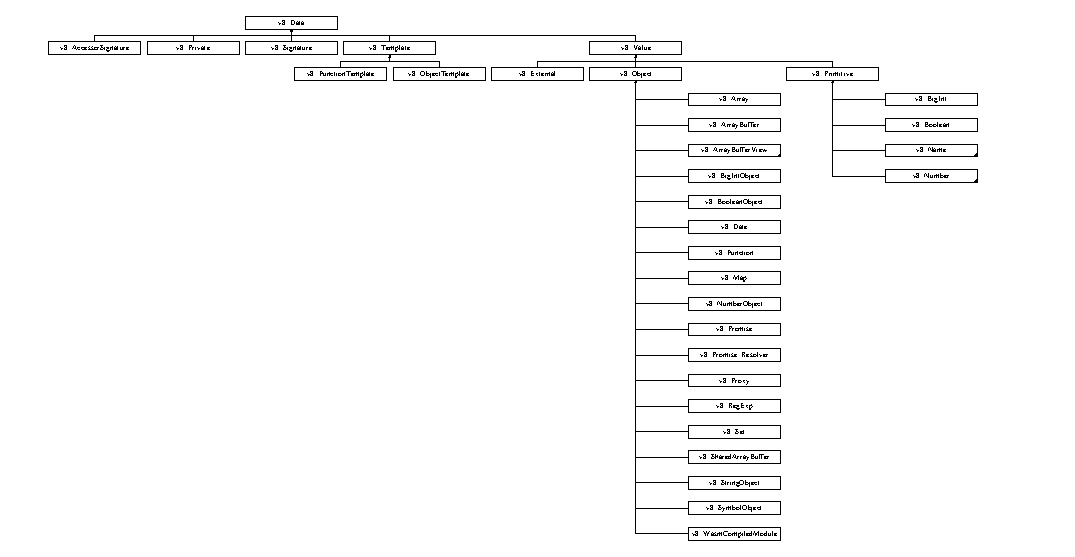
\includegraphics[height=6.491763cm]{classv8_1_1Data}
\end{center}
\end{figure}


\subsection{Detailed Description}
The superclass of values and A\+PI object templates. 

The documentation for this class was generated from the following file\+:\begin{DoxyCompactItemize}
\item 
v8/include/v8.\+h\end{DoxyCompactItemize}

\hypertarget{classv8_1_1DataView}{}\section{v8\+:\+:Data\+View Class Reference}
\label{classv8_1_1DataView}\index{v8\+::\+Data\+View@{v8\+::\+Data\+View}}


{\ttfamily \#include $<$v8.\+h$>$}

Inheritance diagram for v8\+:\+:Data\+View\+:\begin{figure}[H]
\begin{center}
\leavevmode
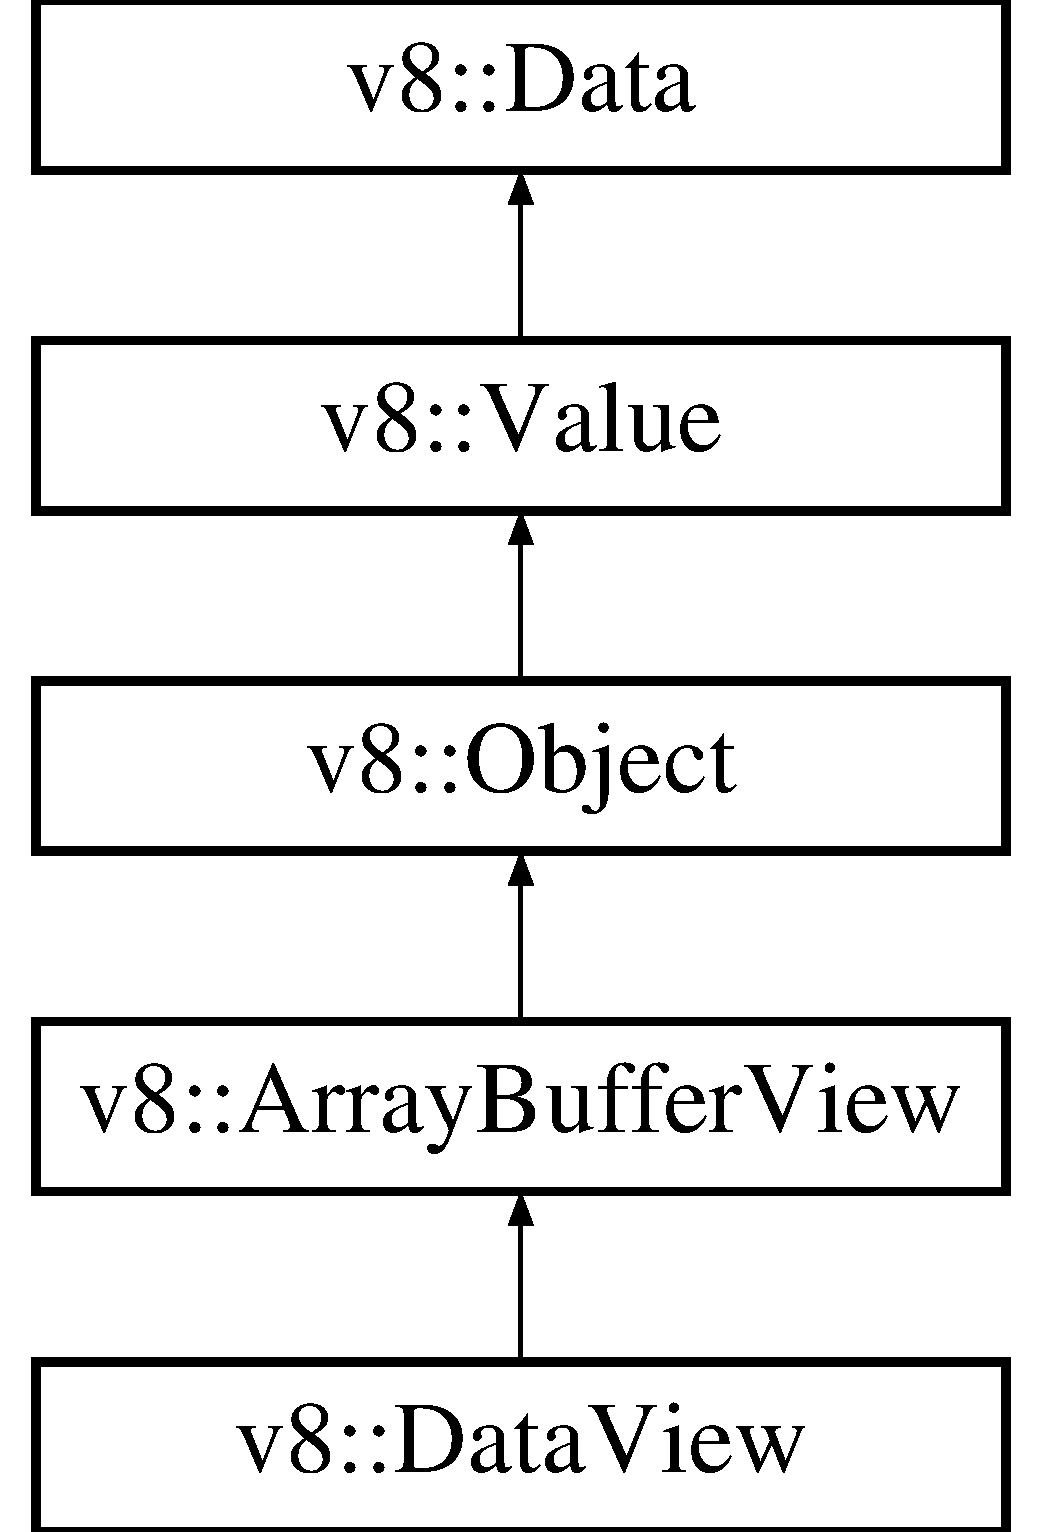
\includegraphics[height=5.000000cm]{classv8_1_1DataView}
\end{center}
\end{figure}
\subsection*{Static Public Member Functions}
\begin{DoxyCompactItemize}
\item 
\mbox{\Hypertarget{classv8_1_1DataView_a40dcfc9ed56dbc41f48ddc49271cbab0}\label{classv8_1_1DataView_a40dcfc9ed56dbc41f48ddc49271cbab0}} 
static \mbox{\hyperlink{classv8_1_1Local}{Local}}$<$ \mbox{\hyperlink{classv8_1_1DataView}{Data\+View}} $>$ {\bfseries New} (\mbox{\hyperlink{classv8_1_1Local}{Local}}$<$ \mbox{\hyperlink{classv8_1_1ArrayBuffer}{Array\+Buffer}} $>$ array\+\_\+buffer, size\+\_\+t byte\+\_\+offset, size\+\_\+t length)
\item 
\mbox{\Hypertarget{classv8_1_1DataView_a8310e075564dd9f26122be2733995ba2}\label{classv8_1_1DataView_a8310e075564dd9f26122be2733995ba2}} 
static \mbox{\hyperlink{classv8_1_1Local}{Local}}$<$ \mbox{\hyperlink{classv8_1_1DataView}{Data\+View}} $>$ {\bfseries New} (\mbox{\hyperlink{classv8_1_1Local}{Local}}$<$ \mbox{\hyperlink{classv8_1_1SharedArrayBuffer}{Shared\+Array\+Buffer}} $>$ shared\+\_\+array\+\_\+buffer, size\+\_\+t byte\+\_\+offset, size\+\_\+t length)
\item 
\mbox{\Hypertarget{classv8_1_1DataView_aa97d15fcb28c6c002a52d32877c8fd3a}\label{classv8_1_1DataView_aa97d15fcb28c6c002a52d32877c8fd3a}} 
static V8\+\_\+\+I\+N\+L\+I\+NE \mbox{\hyperlink{classv8_1_1DataView}{Data\+View}} $\ast$ {\bfseries Cast} (\mbox{\hyperlink{classv8_1_1Value}{Value}} $\ast$obj)
\end{DoxyCompactItemize}
\subsection*{Additional Inherited Members}


\subsection{Detailed Description}
An instance of \mbox{\hyperlink{classv8_1_1DataView}{Data\+View}} constructor (E\+S6 draft 15.\+13.\+7). 

The documentation for this class was generated from the following file\+:\begin{DoxyCompactItemize}
\item 
v8/include/v8.\+h\end{DoxyCompactItemize}

\hypertarget{classv8_1_1Date}{}\section{v8\+:\+:Date Class Reference}
\label{classv8_1_1Date}\index{v8\+::\+Date@{v8\+::\+Date}}


{\ttfamily \#include $<$v8.\+h$>$}

Inheritance diagram for v8\+:\+:Date\+:\begin{figure}[H]
\begin{center}
\leavevmode
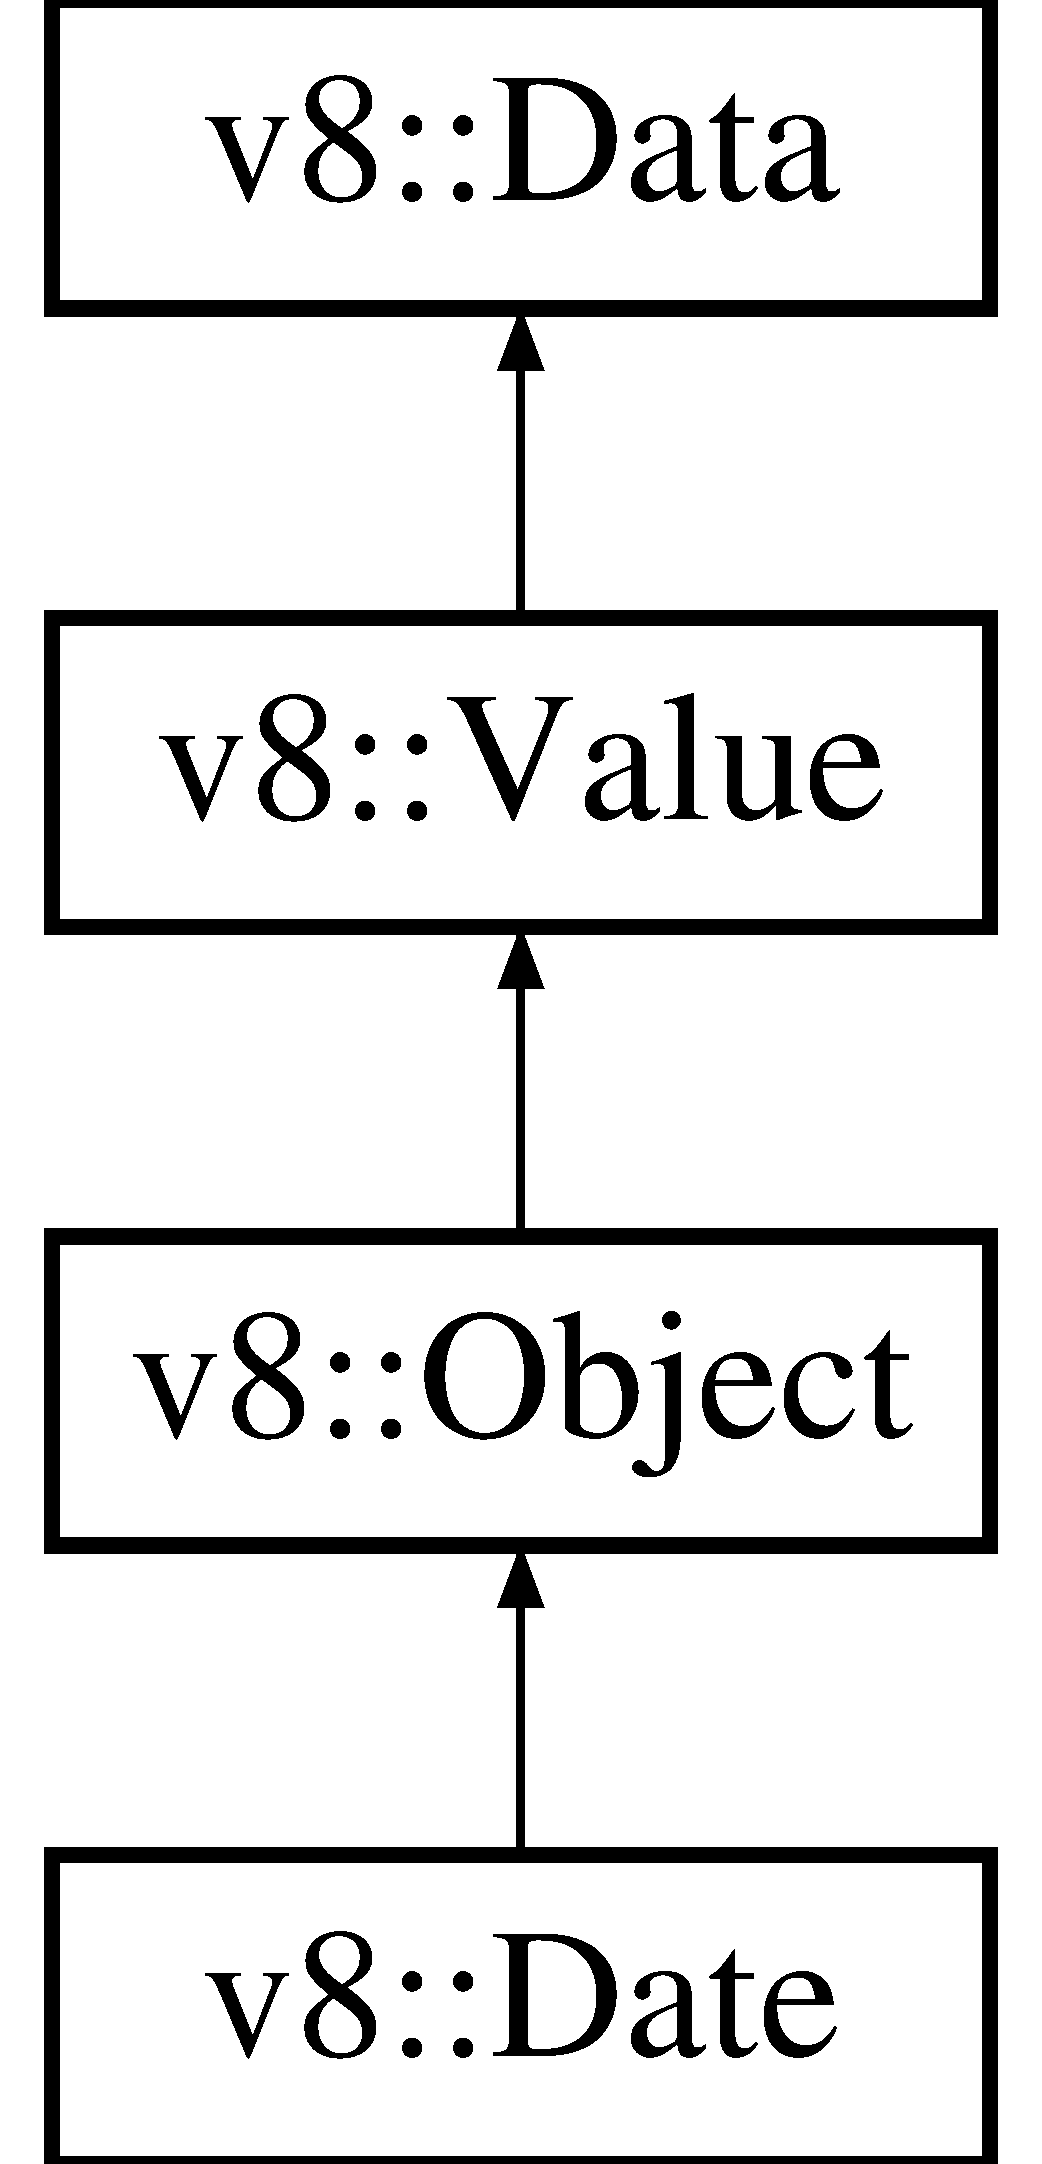
\includegraphics[height=4.000000cm]{classv8_1_1Date}
\end{center}
\end{figure}
\subsection*{Public Member Functions}
\begin{DoxyCompactItemize}
\item 
double \mbox{\hyperlink{classv8_1_1Date_adb9d292549a173e045ee177051dbde19}{Value\+Of}} () const
\end{DoxyCompactItemize}
\subsection*{Static Public Member Functions}
\begin{DoxyCompactItemize}
\item 
\mbox{\Hypertarget{classv8_1_1Date_abd1ff8294e0d5a513696b72b67d36ecf}\label{classv8_1_1Date_abd1ff8294e0d5a513696b72b67d36ecf}} 
static {\bfseries V8\+\_\+\+D\+E\+P\+R\+E\+C\+A\+T\+ED} (\char`\"{}Use maybe version.\char`\"{}, Local$<$ \mbox{\hyperlink{classv8_1_1Value}{Value}} $>$ New(Isolate $\ast$isolate, double time))
\item 
\mbox{\Hypertarget{classv8_1_1Date_a24b0f95c7b9ec5133ad5a983a0a07ce4}\label{classv8_1_1Date_a24b0f95c7b9ec5133ad5a983a0a07ce4}} 
static V8\+\_\+\+W\+A\+R\+N\+\_\+\+U\+N\+U\+S\+E\+D\+\_\+\+R\+E\+S\+U\+LT \mbox{\hyperlink{classv8_1_1MaybeLocal}{Maybe\+Local}}$<$ \mbox{\hyperlink{classv8_1_1Value}{Value}} $>$ {\bfseries New} (\mbox{\hyperlink{classv8_1_1Local}{Local}}$<$ Context $>$ context, double time)
\item 
\mbox{\Hypertarget{classv8_1_1Date_aebb004782ef43f01518f24e662ef6ad8}\label{classv8_1_1Date_aebb004782ef43f01518f24e662ef6ad8}} 
static V8\+\_\+\+I\+N\+L\+I\+NE \mbox{\hyperlink{classv8_1_1Date}{Date}} $\ast$ {\bfseries Cast} (\mbox{\hyperlink{classv8_1_1Value}{Value}} $\ast$obj)
\item 
static void \mbox{\hyperlink{classv8_1_1Date_afa8f4fb31292d1914d9a89fab4fa4415}{Date\+Time\+Configuration\+Change\+Notification}} (Isolate $\ast$isolate)
\end{DoxyCompactItemize}


\subsection{Detailed Description}
An instance of the built-\/in \mbox{\hyperlink{classv8_1_1Date}{Date}} constructor (E\+C\+M\+A-\/262, 15.\+9). 

Definition at line 5090 of file v8.\+h.



\subsection{Member Function Documentation}
\mbox{\Hypertarget{classv8_1_1Date_afa8f4fb31292d1914d9a89fab4fa4415}\label{classv8_1_1Date_afa8f4fb31292d1914d9a89fab4fa4415}} 
\index{v8\+::\+Date@{v8\+::\+Date}!Date\+Time\+Configuration\+Change\+Notification@{Date\+Time\+Configuration\+Change\+Notification}}
\index{Date\+Time\+Configuration\+Change\+Notification@{Date\+Time\+Configuration\+Change\+Notification}!v8\+::\+Date@{v8\+::\+Date}}
\subsubsection{\texorpdfstring{Date\+Time\+Configuration\+Change\+Notification()}{DateTimeConfigurationChangeNotification()}}
{\footnotesize\ttfamily void v8\+::\+Date\+::\+Date\+Time\+Configuration\+Change\+Notification (\begin{DoxyParamCaption}\item[{Isolate $\ast$}]{isolate }\end{DoxyParamCaption})\hspace{0.3cm}{\ttfamily [static]}}

Notification that the embedder has changed the time zone, daylight savings time, or other date / time configuration parameters. V8 keeps a cache of various values used for date / time computation. This notification will reset those cached values for the current context so that date / time configuration changes would be reflected in the \mbox{\hyperlink{classv8_1_1Date}{Date}} object.

This A\+PI should not be called more than needed as it will negatively impact the performance of date operations. 

Definition at line 6912 of file api.\+cc.

\mbox{\Hypertarget{classv8_1_1Date_adb9d292549a173e045ee177051dbde19}\label{classv8_1_1Date_adb9d292549a173e045ee177051dbde19}} 
\index{v8\+::\+Date@{v8\+::\+Date}!Value\+Of@{Value\+Of}}
\index{Value\+Of@{Value\+Of}!v8\+::\+Date@{v8\+::\+Date}}
\subsubsection{\texorpdfstring{Value\+Of()}{ValueOf()}}
{\footnotesize\ttfamily double v8\+::\+Date\+::\+Value\+Of (\begin{DoxyParamCaption}{ }\end{DoxyParamCaption}) const}

A specialization of Value\+::\+Number\+Value that is more efficient because we know the structure of this object. 

Definition at line 6903 of file api.\+cc.



The documentation for this class was generated from the following files\+:\begin{DoxyCompactItemize}
\item 
v8/include/v8.\+h\item 
v8/src/api.\+cc\end{DoxyCompactItemize}

\hypertarget{classv8_1_1Debug}{}\section{v8\+:\+:Debug Class Reference}
\label{classv8_1_1Debug}\index{v8\+::\+Debug@{v8\+::\+Debug}}
\subsection*{Data Structures}
\begin{DoxyCompactItemize}
\item 
class \hyperlink{classv8_1_1Debug_1_1ClientData}{Client\+Data}
\item 
class \hyperlink{classv8_1_1Debug_1_1EventDetails}{Event\+Details}
\item 
class \hyperlink{classv8_1_1Debug_1_1Message}{Message}
\end{DoxyCompactItemize}
\subsection*{Public Types}
\begin{DoxyCompactItemize}
\item 
typedef void($\ast$ \hyperlink{classv8_1_1Debug_ab53894746a21222796062f0e81ea28d8}{Event\+Callback}) (const \hyperlink{classv8_1_1Debug_1_1EventDetails}{Event\+Details} \&event\+\_\+details)
\item 
typedef void($\ast$ \hyperlink{classv8_1_1Debug_a526826b857bd3e3efa184e12bcebc694}{Message\+Handler}) (const \hyperlink{classv8_1_1Debug_1_1Message}{Message} \&message)
\item 
typedef void($\ast$ \hyperlink{classv8_1_1Debug_a91cd8aa9743e3478bc63fe73abcd557c}{Debug\+Message\+Dispatch\+Handler}) ()
\end{DoxyCompactItemize}
\subsection*{Public Member Functions}
\begin{DoxyCompactItemize}
\item 
{\bfseries V8\+\_\+\+D\+E\+P\+R\+E\+C\+A\+T\+ED} (\char`\"{}Use version with an \hyperlink{classv8_1_1Isolate}{Isolate}\char`\"{}, static bool Set\+Debug\+Event\+Listener(                                                                       \hyperlink{classv8_1_1Debug_ab53894746a21222796062f0e81ea28d8}{Event\+Callback} that, \hyperlink{classv8_1_1Local}{Local}$<$ \hyperlink{classv8_1_1Value}{Value} $>$ data=\hyperlink{classv8_1_1Local}{Local}$<$ \hyperlink{classv8_1_1Value}{Value} $>$()))\hypertarget{classv8_1_1Debug_a136072a1c36660385a4dd5e242588eff}{}\label{classv8_1_1Debug_a136072a1c36660385a4dd5e242588eff}

\item 
{\bfseries V8\+\_\+\+D\+E\+P\+R\+E\+C\+A\+T\+ED} (\char`\"{}Use version with an \hyperlink{classv8_1_1Isolate}{Isolate}\char`\"{}, static void Set\+Message\+Handler(\hyperlink{classv8_1_1Debug_a526826b857bd3e3efa184e12bcebc694}{Message\+Handler} handler))\hypertarget{classv8_1_1Debug_a47ea3e258dfe3539890b4a29859481e4}{}\label{classv8_1_1Debug_a47ea3e258dfe3539890b4a29859481e4}

\item 
{\bfseries V8\+\_\+\+D\+E\+P\+R\+E\+C\+A\+T\+ED} (\char`\"{}Use version with an \hyperlink{classv8_1_1Isolate}{Isolate}\char`\"{}, static void \hyperlink{classv8_1_1Debug_af005b911101260e0458847d149d5610e}{Process\+Debug\+Messages}())\hypertarget{classv8_1_1Debug_a5682cd506adcc344fe99b8c9b21bbac8}{}\label{classv8_1_1Debug_a5682cd506adcc344fe99b8c9b21bbac8}

\item 
{\bfseries V8\+\_\+\+D\+E\+P\+R\+E\+C\+A\+T\+ED} (\char`\"{}Use version with an \hyperlink{classv8_1_1Isolate}{Isolate}\char`\"{}, static \hyperlink{classv8_1_1Local}{Local}$<$ \hyperlink{classv8_1_1Context}{Context} $>$ \hyperlink{classv8_1_1Debug_abcf6727d68c5f8c35eef75a72e6a0da8}{Get\+Debug\+Context}())\hypertarget{classv8_1_1Debug_afe8bf40a79b8769cedfb7aafef74e77f}{}\label{classv8_1_1Debug_afe8bf40a79b8769cedfb7aafef74e77f}

\end{DoxyCompactItemize}
\subsection*{Static Public Member Functions}
\begin{DoxyCompactItemize}
\item 
static bool {\bfseries Set\+Debug\+Event\+Listener} (\hyperlink{classv8_1_1Isolate}{Isolate} $\ast$isolate, \hyperlink{classv8_1_1Debug_ab53894746a21222796062f0e81ea28d8}{Event\+Callback} that, \hyperlink{classv8_1_1Local}{Local}$<$ \hyperlink{classv8_1_1Value}{Value} $>$ data=\hyperlink{classv8_1_1Local}{Local}$<$ \hyperlink{classv8_1_1Value}{Value} $>$())\hypertarget{classv8_1_1Debug_a7f5138bd280a4c3fa9058a2d559687dd}{}\label{classv8_1_1Debug_a7f5138bd280a4c3fa9058a2d559687dd}

\item 
static void {\bfseries Debug\+Break} (\hyperlink{classv8_1_1Isolate}{Isolate} $\ast$isolate)\hypertarget{classv8_1_1Debug_a0c730ea558b1fc86cb728980c91a4c7c}{}\label{classv8_1_1Debug_a0c730ea558b1fc86cb728980c91a4c7c}

\item 
static void {\bfseries Cancel\+Debug\+Break} (\hyperlink{classv8_1_1Isolate}{Isolate} $\ast$isolate)\hypertarget{classv8_1_1Debug_a976a373dc06c146cdbe8d6f2fd7f57b5}{}\label{classv8_1_1Debug_a976a373dc06c146cdbe8d6f2fd7f57b5}

\item 
static bool {\bfseries Check\+Debug\+Break} (\hyperlink{classv8_1_1Isolate}{Isolate} $\ast$isolate)\hypertarget{classv8_1_1Debug_aa564431664efa61d6d72c9cbd91b4ea2}{}\label{classv8_1_1Debug_aa564431664efa61d6d72c9cbd91b4ea2}

\item 
static void {\bfseries Set\+Message\+Handler} (\hyperlink{classv8_1_1Isolate}{Isolate} $\ast$isolate, \hyperlink{classv8_1_1Debug_a526826b857bd3e3efa184e12bcebc694}{Message\+Handler} handler)\hypertarget{classv8_1_1Debug_ae49147c056122437bacc3d26cc349125}{}\label{classv8_1_1Debug_ae49147c056122437bacc3d26cc349125}

\item 
static void {\bfseries Send\+Command} (\hyperlink{classv8_1_1Isolate}{Isolate} $\ast$isolate, const uint16\+\_\+t $\ast$command, int length, \hyperlink{classv8_1_1Debug_1_1ClientData}{Client\+Data} $\ast$client\+\_\+data=N\+U\+LL)\hypertarget{classv8_1_1Debug_aba2426f25ee7cd31659426287777bb00}{}\label{classv8_1_1Debug_aba2426f25ee7cd31659426287777bb00}

\item 
static \hyperlink{classv8_1_1Debug_a5c53fc48b3fca71b6397cfecd1c82a9d}{V8\+\_\+\+D\+E\+P\+R\+E\+C\+A\+T\+ED} (\char`\"{}Use maybe version\char`\"{}, Local$<$ \hyperlink{classv8_1_1Value}{Value} $>$ Call(\hyperlink{classv8_1_1Local}{v8\+::\+Local}$<$ \hyperlink{classv8_1_1Function}{v8\+::\+Function} $>$ fun,                                                                                                                                                           \hyperlink{classv8_1_1Local}{Local}$<$ \hyperlink{classv8_1_1Value}{Value} $>$ data=\hyperlink{classv8_1_1Local}{Local}$<$ \hyperlink{classv8_1_1Value}{Value} $>$()))
\item 
static \hyperlink{classv8_1_1MaybeLocal}{Maybe\+Local}$<$ \hyperlink{classv8_1_1Value}{Value} $>$ {\bfseries Call} (\hyperlink{classv8_1_1Local}{Local}$<$ \hyperlink{classv8_1_1Context}{Context} $>$ context, \hyperlink{classv8_1_1Local}{v8\+::\+Local}$<$ \hyperlink{classv8_1_1Function}{v8\+::\+Function} $>$ fun, \hyperlink{classv8_1_1Local}{Local}$<$ \hyperlink{classv8_1_1Value}{Value} $>$ data=\hyperlink{classv8_1_1Local}{Local}$<$ \hyperlink{classv8_1_1Value}{Value} $>$())\hypertarget{classv8_1_1Debug_a32e28ec40dc429e7fa1dfbe1e514ba3d}{}\label{classv8_1_1Debug_a32e28ec40dc429e7fa1dfbe1e514ba3d}

\item 
static \hyperlink{classv8_1_1Debug_aeda86872fb9c66df641e6d16c8db7182}{V8\+\_\+\+D\+E\+P\+R\+E\+C\+A\+T\+ED} (\char`\"{}Use maybe version\char`\"{}, Local$<$ \hyperlink{classv8_1_1Value}{Value} $>$ Get\+Mirror(\hyperlink{classv8_1_1Local}{v8\+::\+Local}$<$ \hyperlink{classv8_1_1Value}{v8\+::\+Value} $>$ obj))
\item 
static \hyperlink{classv8_1_1MaybeLocal}{Maybe\+Local}$<$ \hyperlink{classv8_1_1Value}{Value} $>$ {\bfseries Get\+Mirror} (\hyperlink{classv8_1_1Local}{Local}$<$ \hyperlink{classv8_1_1Context}{Context} $>$ context, \hyperlink{classv8_1_1Local}{v8\+::\+Local}$<$ \hyperlink{classv8_1_1Value}{v8\+::\+Value} $>$ obj)\hypertarget{classv8_1_1Debug_ab5f5ae3f4418c576da4633c6fb27b23d}{}\label{classv8_1_1Debug_ab5f5ae3f4418c576da4633c6fb27b23d}

\item 
static void \hyperlink{classv8_1_1Debug_af005b911101260e0458847d149d5610e}{Process\+Debug\+Messages} (\hyperlink{classv8_1_1Isolate}{Isolate} $\ast$isolate)
\item 
static \hyperlink{classv8_1_1Local}{Local}$<$ \hyperlink{classv8_1_1Context}{Context} $>$ \hyperlink{classv8_1_1Debug_abcf6727d68c5f8c35eef75a72e6a0da8}{Get\+Debug\+Context} (\hyperlink{classv8_1_1Isolate}{Isolate} $\ast$isolate)
\item 
static void \hyperlink{classv8_1_1Debug_ab635f979d369bed13187e2594d825517}{Set\+Live\+Edit\+Enabled} (\hyperlink{classv8_1_1Isolate}{Isolate} $\ast$isolate, bool enable)
\item 
static \hyperlink{classv8_1_1MaybeLocal}{Maybe\+Local}$<$ \hyperlink{classv8_1_1Array}{Array} $>$ \hyperlink{classv8_1_1Debug_a10ef14b11ffdd57287f25b39dc728e07}{Get\+Internal\+Properties} (\hyperlink{classv8_1_1Isolate}{Isolate} $\ast$isolate, \hyperlink{classv8_1_1Local}{Local}$<$ \hyperlink{classv8_1_1Value}{Value} $>$ value)
\item 
static bool \hyperlink{classv8_1_1Debug_a79ce7b9e4e09be64ca1c3494ec6130ab}{Is\+Tail\+Call\+Elimination\+Enabled} (\hyperlink{classv8_1_1Isolate}{Isolate} $\ast$isolate)
\item 
static void {\bfseries Set\+Tail\+Call\+Elimination\+Enabled} (\hyperlink{classv8_1_1Isolate}{Isolate} $\ast$isolate, bool enabled)\hypertarget{classv8_1_1Debug_a06662e09d22d6eaed81f20824066cea5}{}\label{classv8_1_1Debug_a06662e09d22d6eaed81f20824066cea5}

\end{DoxyCompactItemize}


\subsection{Member Typedef Documentation}
\index{v8\+::\+Debug@{v8\+::\+Debug}!Debug\+Message\+Dispatch\+Handler@{Debug\+Message\+Dispatch\+Handler}}
\index{Debug\+Message\+Dispatch\+Handler@{Debug\+Message\+Dispatch\+Handler}!v8\+::\+Debug@{v8\+::\+Debug}}
\subsubsection[{\texorpdfstring{Debug\+Message\+Dispatch\+Handler}{DebugMessageDispatchHandler}}]{\setlength{\rightskip}{0pt plus 5cm}typedef void($\ast$ v8\+::\+Debug\+::\+Debug\+Message\+Dispatch\+Handler) ()}\hypertarget{classv8_1_1Debug_a91cd8aa9743e3478bc63fe73abcd557c}{}\label{classv8_1_1Debug_a91cd8aa9743e3478bc63fe73abcd557c}
Callback function for the host to ensure debug messages are processed. \index{v8\+::\+Debug@{v8\+::\+Debug}!Event\+Callback@{Event\+Callback}}
\index{Event\+Callback@{Event\+Callback}!v8\+::\+Debug@{v8\+::\+Debug}}
\subsubsection[{\texorpdfstring{Event\+Callback}{EventCallback}}]{\setlength{\rightskip}{0pt plus 5cm}typedef void($\ast$ v8\+::\+Debug\+::\+Event\+Callback) (const {\bf Event\+Details} \&event\+\_\+details)}\hypertarget{classv8_1_1Debug_ab53894746a21222796062f0e81ea28d8}{}\label{classv8_1_1Debug_ab53894746a21222796062f0e81ea28d8}
\hyperlink{classv8_1_1Debug}{Debug} event callback function.


\begin{DoxyParams}{Parameters}
{\em event\+\_\+details} & object providing information about the debug event\\
\hline
\end{DoxyParams}
A Event\+Callback2 does not take possession of the event data, and must not rely on the data persisting after the handler returns. \index{v8\+::\+Debug@{v8\+::\+Debug}!Message\+Handler@{Message\+Handler}}
\index{Message\+Handler@{Message\+Handler}!v8\+::\+Debug@{v8\+::\+Debug}}
\subsubsection[{\texorpdfstring{Message\+Handler}{MessageHandler}}]{\setlength{\rightskip}{0pt plus 5cm}typedef void($\ast$ v8\+::\+Debug\+::\+Message\+Handler) (const {\bf Message} \&message)}\hypertarget{classv8_1_1Debug_a526826b857bd3e3efa184e12bcebc694}{}\label{classv8_1_1Debug_a526826b857bd3e3efa184e12bcebc694}
\hyperlink{classv8_1_1Debug}{Debug} message callback function.


\begin{DoxyParams}{Parameters}
{\em message} & the debug message handler message object\\
\hline
\end{DoxyParams}
A Message\+Handler2 does not take possession of the message data, and must not rely on the data persisting after the handler returns. 

\subsection{Member Function Documentation}
\index{v8\+::\+Debug@{v8\+::\+Debug}!Get\+Debug\+Context@{Get\+Debug\+Context}}
\index{Get\+Debug\+Context@{Get\+Debug\+Context}!v8\+::\+Debug@{v8\+::\+Debug}}
\subsubsection[{\texorpdfstring{Get\+Debug\+Context(\+Isolate $\ast$isolate)}{GetDebugContext(Isolate *isolate)}}]{\setlength{\rightskip}{0pt plus 5cm}static {\bf Local}$<${\bf Context}$>$ v8\+::\+Debug\+::\+Get\+Debug\+Context (
\begin{DoxyParamCaption}
\item[{{\bf Isolate} $\ast$}]{isolate}
\end{DoxyParamCaption}
)\hspace{0.3cm}{\ttfamily [static]}}\hypertarget{classv8_1_1Debug_abcf6727d68c5f8c35eef75a72e6a0da8}{}\label{classv8_1_1Debug_abcf6727d68c5f8c35eef75a72e6a0da8}
Debugger is running in its own context which is entered while debugger messages are being dispatched. This is an explicit getter for this debugger context. Note that the content of the debugger context is subject to change. The \hyperlink{classv8_1_1Context}{Context} exists only when the debugger is active, i.\+e. at least one Debug\+Event\+Listener or Message\+Handler is set. \index{v8\+::\+Debug@{v8\+::\+Debug}!Get\+Internal\+Properties@{Get\+Internal\+Properties}}
\index{Get\+Internal\+Properties@{Get\+Internal\+Properties}!v8\+::\+Debug@{v8\+::\+Debug}}
\subsubsection[{\texorpdfstring{Get\+Internal\+Properties(\+Isolate $\ast$isolate, Local$<$ Value $>$ value)}{GetInternalProperties(Isolate *isolate, Local< Value > value)}}]{\setlength{\rightskip}{0pt plus 5cm}static {\bf Maybe\+Local}$<${\bf Array}$>$ v8\+::\+Debug\+::\+Get\+Internal\+Properties (
\begin{DoxyParamCaption}
\item[{{\bf Isolate} $\ast$}]{isolate, }
\item[{{\bf Local}$<$ {\bf Value} $>$}]{value}
\end{DoxyParamCaption}
)\hspace{0.3cm}{\ttfamily [static]}}\hypertarget{classv8_1_1Debug_a10ef14b11ffdd57287f25b39dc728e07}{}\label{classv8_1_1Debug_a10ef14b11ffdd57287f25b39dc728e07}
Returns array of internal properties specific to the value type. Result has the following format\+: \mbox{[}$<$name$>$, 

,...,$<$name$>$, 

\mbox{]}. Result array will be allocated in the current context. \index{v8\+::\+Debug@{v8\+::\+Debug}!Is\+Tail\+Call\+Elimination\+Enabled@{Is\+Tail\+Call\+Elimination\+Enabled}}
\index{Is\+Tail\+Call\+Elimination\+Enabled@{Is\+Tail\+Call\+Elimination\+Enabled}!v8\+::\+Debug@{v8\+::\+Debug}}
\subsubsection[{\texorpdfstring{Is\+Tail\+Call\+Elimination\+Enabled(\+Isolate $\ast$isolate)}{IsTailCallEliminationEnabled(Isolate *isolate)}}]{\setlength{\rightskip}{0pt plus 5cm}static bool v8\+::\+Debug\+::\+Is\+Tail\+Call\+Elimination\+Enabled (
\begin{DoxyParamCaption}
\item[{{\bf Isolate} $\ast$}]{isolate}
\end{DoxyParamCaption}
)\hspace{0.3cm}{\ttfamily [static]}}\hypertarget{classv8_1_1Debug_a79ce7b9e4e09be64ca1c3494ec6130ab}{}\label{classv8_1_1Debug_a79ce7b9e4e09be64ca1c3494ec6130ab}
Defines if the E\+S2015 tail call elimination feature is enabled or not. The change of this flag triggers deoptimization of all functions that contain calls at tail position. \index{v8\+::\+Debug@{v8\+::\+Debug}!Process\+Debug\+Messages@{Process\+Debug\+Messages}}
\index{Process\+Debug\+Messages@{Process\+Debug\+Messages}!v8\+::\+Debug@{v8\+::\+Debug}}
\subsubsection[{\texorpdfstring{Process\+Debug\+Messages(\+Isolate $\ast$isolate)}{ProcessDebugMessages(Isolate *isolate)}}]{\setlength{\rightskip}{0pt plus 5cm}static void v8\+::\+Debug\+::\+Process\+Debug\+Messages (
\begin{DoxyParamCaption}
\item[{{\bf Isolate} $\ast$}]{isolate}
\end{DoxyParamCaption}
)\hspace{0.3cm}{\ttfamily [static]}}\hypertarget{classv8_1_1Debug_af005b911101260e0458847d149d5610e}{}\label{classv8_1_1Debug_af005b911101260e0458847d149d5610e}
Makes \hyperlink{classv8_1_1V8}{V8} process all pending debug messages.

From \hyperlink{classv8_1_1V8}{V8} point of view all debug messages come asynchronously (e.\+g. from remote debugger) but they all must be handled synchronously\+: \hyperlink{classv8_1_1V8}{V8} cannot do 2 things at one time so normal script execution must be interrupted for a while.

Generally when message arrives \hyperlink{classv8_1_1V8}{V8} may be in one of 3 states\+:
\begin{DoxyEnumerate}
\item \hyperlink{classv8_1_1V8}{V8} is running script; \hyperlink{classv8_1_1V8}{V8} will automatically interrupt and process all pending messages;
\item \hyperlink{classv8_1_1V8}{V8} is suspended on debug breakpoint; in this state \hyperlink{classv8_1_1V8}{V8} is dedicated to reading and processing debug messages;
\item \hyperlink{classv8_1_1V8}{V8} is not running at all or has called some long-\/working C++ function; by default it means that processing of all debug messages will be deferred until \hyperlink{classv8_1_1V8}{V8} gets control again; however, embedding application may improve this by manually calling this method.
\end{DoxyEnumerate}

Technically this method in many senses is equivalent to executing empty script\+:
\begin{DoxyEnumerate}
\item It does nothing except for processing all pending debug messages.
\item It should be invoked with the same precautions and from the same context as \hyperlink{classv8_1_1V8}{V8} script would be invoked from, because\+: a. with \char`\"{}evaluate\char`\"{} command it can do whatever normal script can do, including all native calls; b. no other thread should call \hyperlink{classv8_1_1V8}{V8} while this method is running (\hyperlink{classv8_1_1Locker}{v8\+::\+Locker} may be used here).
\end{DoxyEnumerate}

\char`\"{}\+Evaluate\char`\"{} debug command behavior currently is not specified in scope of this method. \index{v8\+::\+Debug@{v8\+::\+Debug}!Set\+Live\+Edit\+Enabled@{Set\+Live\+Edit\+Enabled}}
\index{Set\+Live\+Edit\+Enabled@{Set\+Live\+Edit\+Enabled}!v8\+::\+Debug@{v8\+::\+Debug}}
\subsubsection[{\texorpdfstring{Set\+Live\+Edit\+Enabled(\+Isolate $\ast$isolate, bool enable)}{SetLiveEditEnabled(Isolate *isolate, bool enable)}}]{\setlength{\rightskip}{0pt plus 5cm}static void v8\+::\+Debug\+::\+Set\+Live\+Edit\+Enabled (
\begin{DoxyParamCaption}
\item[{{\bf Isolate} $\ast$}]{isolate, }
\item[{bool}]{enable}
\end{DoxyParamCaption}
)\hspace{0.3cm}{\ttfamily [static]}}\hypertarget{classv8_1_1Debug_ab635f979d369bed13187e2594d825517}{}\label{classv8_1_1Debug_ab635f979d369bed13187e2594d825517}
Enable/disable Live\+Edit functionality for the given \hyperlink{classv8_1_1Isolate}{Isolate} (default \hyperlink{classv8_1_1Isolate}{Isolate} if not provided). \hyperlink{classv8_1_1V8}{V8} will abort if Live\+Edit is unexpectedly used. Live\+Edit is enabled by default. \index{v8\+::\+Debug@{v8\+::\+Debug}!V8\+\_\+\+D\+E\+P\+R\+E\+C\+A\+T\+ED@{V8\+\_\+\+D\+E\+P\+R\+E\+C\+A\+T\+ED}}
\index{V8\+\_\+\+D\+E\+P\+R\+E\+C\+A\+T\+ED@{V8\+\_\+\+D\+E\+P\+R\+E\+C\+A\+T\+ED}!v8\+::\+Debug@{v8\+::\+Debug}}
\subsubsection[{\texorpdfstring{V8\+\_\+\+D\+E\+P\+R\+E\+C\+A\+T\+E\+D(""Use maybe version"", Local$<$ Value $>$ Call(v8\+::\+Local$<$ v8\+::\+Function $>$ fun,                                                                                                                                                           Local$<$ Value $>$ data=\+Local$<$ Value $>$()))}{V8_DEPRECATED("Use maybe version", Local< Value > Call(v8::Local< v8::Function > fun,                                                                                                                                                           Local< Value > data=Local< Value >()))}}]{\setlength{\rightskip}{0pt plus 5cm}static v8\+::\+Debug\+::\+V8\+\_\+\+D\+E\+P\+R\+E\+C\+A\+T\+ED (
\begin{DoxyParamCaption}
\item[{\char`\"{}Use maybe version\char`\"{}}]{, }
\item[{{\bf Local}$<$ {\bf Value} $>$ }]{Callv8\+::\+Local$<$ v8\+::\+Function $>$ fun,                                                                                                                                                                                                                                                                                                                   Local$<$ Value $>$ data=\+Local$<$ Value $>$()}
\end{DoxyParamCaption}
)\hspace{0.3cm}{\ttfamily [static]}}\hypertarget{classv8_1_1Debug_a5c53fc48b3fca71b6397cfecd1c82a9d}{}\label{classv8_1_1Debug_a5c53fc48b3fca71b6397cfecd1c82a9d}
Run a Java\+Script function in the debugger. 
\begin{DoxyParams}{Parameters}
{\em fun} & the function to call \\
\hline
{\em data} & passed as second argument to the function With this call the debugger is entered and the function specified is called with the execution state as the first argument. This makes it possible to get access to information otherwise not available during normal Java\+Script execution e.\+g. details on stack frames. Receiver of the function call will be the debugger context global object, however this is a subject to change. The following example shows a Java\+Script function which when passed to v8\+::\+Debug\+::\+Call will return the current line of Java\+Script execution.\\
\hline
\end{DoxyParams}

\begin{DoxyCode}
\textcolor{keyword}{function} frame\_source\_line(exec\_state) \{
  \textcolor{keywordflow}{return} exec\_state.frame(0).sourceLine();
\}
\end{DoxyCode}
 \index{v8\+::\+Debug@{v8\+::\+Debug}!V8\+\_\+\+D\+E\+P\+R\+E\+C\+A\+T\+ED@{V8\+\_\+\+D\+E\+P\+R\+E\+C\+A\+T\+ED}}
\index{V8\+\_\+\+D\+E\+P\+R\+E\+C\+A\+T\+ED@{V8\+\_\+\+D\+E\+P\+R\+E\+C\+A\+T\+ED}!v8\+::\+Debug@{v8\+::\+Debug}}
\subsubsection[{\texorpdfstring{V8\+\_\+\+D\+E\+P\+R\+E\+C\+A\+T\+E\+D(""Use maybe version"", Local$<$ Value $>$ Get\+Mirror(v8\+::\+Local$<$ v8\+::\+Value $>$ obj))}{V8_DEPRECATED("Use maybe version", Local< Value > GetMirror(v8::Local< v8::Value > obj))}}]{\setlength{\rightskip}{0pt plus 5cm}static v8\+::\+Debug\+::\+V8\+\_\+\+D\+E\+P\+R\+E\+C\+A\+T\+ED (
\begin{DoxyParamCaption}
\item[{\char`\"{}Use maybe version\char`\"{}}]{, }
\item[{{\bf Local}$<$ {\bf Value} $>$ }]{Get\+Mirrorv8\+::\+Local$<$ v8\+::\+Value $>$ obj}
\end{DoxyParamCaption}
)\hspace{0.3cm}{\ttfamily [static]}}\hypertarget{classv8_1_1Debug_aeda86872fb9c66df641e6d16c8db7182}{}\label{classv8_1_1Debug_aeda86872fb9c66df641e6d16c8db7182}
Returns a mirror object for the given object. 

The documentation for this class was generated from the following file\+:\begin{DoxyCompactItemize}
\item 
v8/include/v8-\/debug.\+h\end{DoxyCompactItemize}

\hypertarget{classv8_1_1DefaultGlobalMapTraits}{}\section{v8\+:\+:Default\+Global\+Map\+Traits$<$ K, V $>$ Class Template Reference}
\label{classv8_1_1DefaultGlobalMapTraits}\index{v8\+::\+Default\+Global\+Map\+Traits$<$ K, V $>$@{v8\+::\+Default\+Global\+Map\+Traits$<$ K, V $>$}}
Inheritance diagram for v8\+:\+:Default\+Global\+Map\+Traits$<$ K, V $>$\+:\begin{figure}[H]
\begin{center}
\leavevmode
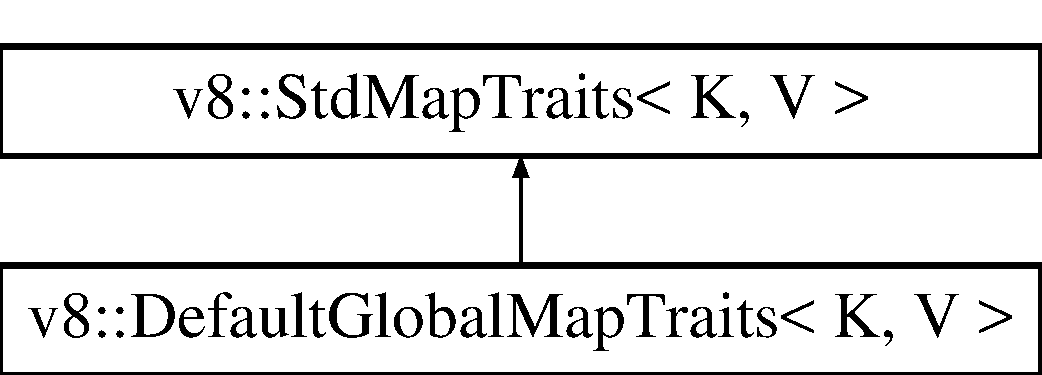
\includegraphics[height=2.000000cm]{classv8_1_1DefaultGlobalMapTraits}
\end{center}
\end{figure}
\subsection*{Public Types}
\begin{DoxyCompactItemize}
\item 
\mbox{\Hypertarget{classv8_1_1DefaultGlobalMapTraits_a6626b089621a436fde5ac1a1132cc83c}\label{classv8_1_1DefaultGlobalMapTraits_a6626b089621a436fde5ac1a1132cc83c}} 
typedef \mbox{\hyperlink{classv8_1_1GlobalValueMap}{Global\+Value\+Map}}$<$ K, \mbox{\hyperlink{classV}{V}}, \mbox{\hyperlink{classv8_1_1DefaultGlobalMapTraits}{Default\+Global\+Map\+Traits}}$<$ K, \mbox{\hyperlink{classV}{V}} $>$ $>$ {\bfseries Map\+Type}
\item 
\mbox{\Hypertarget{classv8_1_1DefaultGlobalMapTraits_af5285197aae83dcb00d0381fbc90869e}\label{classv8_1_1DefaultGlobalMapTraits_af5285197aae83dcb00d0381fbc90869e}} 
typedef void {\bfseries Weak\+Callback\+Data\+Type}
\end{DoxyCompactItemize}
\subsection*{Static Public Member Functions}
\begin{DoxyCompactItemize}
\item 
\mbox{\Hypertarget{classv8_1_1DefaultGlobalMapTraits_a3d4b483a077d6e5665cc62a23c719ee8}\label{classv8_1_1DefaultGlobalMapTraits_a3d4b483a077d6e5665cc62a23c719ee8}} 
static Weak\+Callback\+Data\+Type $\ast$ {\bfseries Weak\+Callback\+Parameter} (\mbox{\hyperlink{classv8_1_1GlobalValueMap}{Map\+Type}} $\ast$map, const K \&key, \mbox{\hyperlink{classv8_1_1Local}{Local}}$<$ \mbox{\hyperlink{classV}{V}} $>$ value)
\item 
\mbox{\Hypertarget{classv8_1_1DefaultGlobalMapTraits_ae65c4d78f93d033712aa328654c00250}\label{classv8_1_1DefaultGlobalMapTraits_ae65c4d78f93d033712aa328654c00250}} 
static \mbox{\hyperlink{classv8_1_1GlobalValueMap}{Map\+Type}} $\ast$ {\bfseries Map\+From\+Weak\+Callback\+Info} (const \mbox{\hyperlink{classv8_1_1WeakCallbackInfo}{Weak\+Callback\+Info}}$<$ Weak\+Callback\+Data\+Type $>$ \&data)
\item 
\mbox{\Hypertarget{classv8_1_1DefaultGlobalMapTraits_a2ebc8d3bbfbe32598863ab44caa36207}\label{classv8_1_1DefaultGlobalMapTraits_a2ebc8d3bbfbe32598863ab44caa36207}} 
static K {\bfseries Key\+From\+Weak\+Callback\+Info} (const \mbox{\hyperlink{classv8_1_1WeakCallbackInfo}{Weak\+Callback\+Info}}$<$ Weak\+Callback\+Data\+Type $>$ \&data)
\item 
\mbox{\Hypertarget{classv8_1_1DefaultGlobalMapTraits_a106883e8168f48826fcfb71aa88e7994}\label{classv8_1_1DefaultGlobalMapTraits_a106883e8168f48826fcfb71aa88e7994}} 
static void {\bfseries Dispose\+Callback\+Data} (Weak\+Callback\+Data\+Type $\ast$data)
\item 
\mbox{\Hypertarget{classv8_1_1DefaultGlobalMapTraits_a2e50fabc65cf498e981015c1e92ece3e}\label{classv8_1_1DefaultGlobalMapTraits_a2e50fabc65cf498e981015c1e92ece3e}} 
static void {\bfseries On\+Weak\+Callback} (const \mbox{\hyperlink{classv8_1_1WeakCallbackInfo}{Weak\+Callback\+Info}}$<$ Weak\+Callback\+Data\+Type $>$ \&data)
\item 
\mbox{\Hypertarget{classv8_1_1DefaultGlobalMapTraits_af2a539ddbe5db2b6e1e944590e1dd7e6}\label{classv8_1_1DefaultGlobalMapTraits_af2a539ddbe5db2b6e1e944590e1dd7e6}} 
static void {\bfseries Dispose} (Isolate $\ast$isolate, \mbox{\hyperlink{classv8_1_1Global}{Global}}$<$ \mbox{\hyperlink{classV}{V}} $>$ value, K key)
\item 
\mbox{\Hypertarget{classv8_1_1DefaultGlobalMapTraits_ad3478535925c0f42664c97c4d35d1c91}\label{classv8_1_1DefaultGlobalMapTraits_ad3478535925c0f42664c97c4d35d1c91}} 
static void {\bfseries Dispose\+Weak} (const \mbox{\hyperlink{classv8_1_1WeakCallbackInfo}{Weak\+Callback\+Info}}$<$ Weak\+Callback\+Data\+Type $>$ \&data)
\end{DoxyCompactItemize}
\subsection*{Static Public Attributes}
\begin{DoxyCompactItemize}
\item 
\mbox{\Hypertarget{classv8_1_1DefaultGlobalMapTraits_aca4a466a95927f10ea3fa0bff1e041d2}\label{classv8_1_1DefaultGlobalMapTraits_aca4a466a95927f10ea3fa0bff1e041d2}} 
static const Persistent\+Container\+Callback\+Type {\bfseries k\+Callback\+Type} = k\+Not\+Weak
\end{DoxyCompactItemize}


\subsection{Detailed Description}
\subsubsection*{template$<$typename K, typename V$>$\newline
class v8\+::\+Default\+Global\+Map\+Traits$<$ K, V $>$}



Definition at line 111 of file v8-\/util.\+h.



The documentation for this class was generated from the following file\+:\begin{DoxyCompactItemize}
\item 
v8/include/v8-\/util.\+h\end{DoxyCompactItemize}

\hypertarget{classv8_1_1DefaultPersistentValueMapTraits}{}\section{v8\+:\+:Default\+Persistent\+Value\+Map\+Traits$<$ K, V $>$ Class Template Reference}
\label{classv8_1_1DefaultPersistentValueMapTraits}\index{v8\+::\+Default\+Persistent\+Value\+Map\+Traits$<$ K, V $>$@{v8\+::\+Default\+Persistent\+Value\+Map\+Traits$<$ K, V $>$}}


{\ttfamily \#include $<$v8-\/util.\+h$>$}

Inheritance diagram for v8\+:\+:Default\+Persistent\+Value\+Map\+Traits$<$ K, V $>$\+:\begin{figure}[H]
\begin{center}
\leavevmode
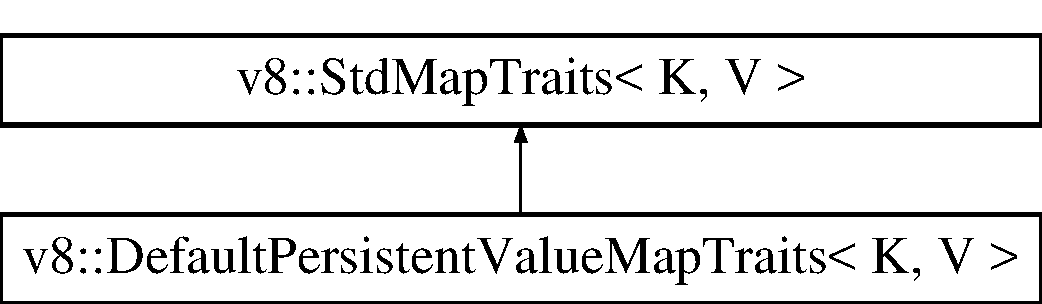
\includegraphics[height=2.000000cm]{classv8_1_1DefaultPersistentValueMapTraits}
\end{center}
\end{figure}
\subsection*{Public Types}
\begin{DoxyCompactItemize}
\item 
\mbox{\Hypertarget{classv8_1_1DefaultPersistentValueMapTraits_a05cbd536d6bb9ba4949198351e074854}\label{classv8_1_1DefaultPersistentValueMapTraits_a05cbd536d6bb9ba4949198351e074854}} 
typedef \mbox{\hyperlink{classv8_1_1PersistentValueMap}{Persistent\+Value\+Map}}$<$ K, \mbox{\hyperlink{classV}{V}}, \mbox{\hyperlink{classv8_1_1DefaultPersistentValueMapTraits}{Default\+Persistent\+Value\+Map\+Traits}}$<$ K, \mbox{\hyperlink{classV}{V}} $>$ $>$ {\bfseries Map\+Type}
\item 
\mbox{\Hypertarget{classv8_1_1DefaultPersistentValueMapTraits_a379f8c42e727a9576fb0954bb0245d8f}\label{classv8_1_1DefaultPersistentValueMapTraits_a379f8c42e727a9576fb0954bb0245d8f}} 
typedef void {\bfseries Weak\+Callback\+Data\+Type}
\end{DoxyCompactItemize}
\subsection*{Static Public Member Functions}
\begin{DoxyCompactItemize}
\item 
\mbox{\Hypertarget{classv8_1_1DefaultPersistentValueMapTraits_a63b6fc80207ce6ac7d1eaa306b68768c}\label{classv8_1_1DefaultPersistentValueMapTraits_a63b6fc80207ce6ac7d1eaa306b68768c}} 
static Weak\+Callback\+Data\+Type $\ast$ {\bfseries Weak\+Callback\+Parameter} (\mbox{\hyperlink{classv8_1_1PersistentValueMap}{Map\+Type}} $\ast$map, const K \&key, \mbox{\hyperlink{classv8_1_1Local}{Local}}$<$ \mbox{\hyperlink{classV}{V}} $>$ value)
\item 
\mbox{\Hypertarget{classv8_1_1DefaultPersistentValueMapTraits_ad5a476677abdec41871199920820e8bd}\label{classv8_1_1DefaultPersistentValueMapTraits_ad5a476677abdec41871199920820e8bd}} 
static \mbox{\hyperlink{classv8_1_1PersistentValueMap}{Map\+Type}} $\ast$ {\bfseries Map\+From\+Weak\+Callback\+Info} (const \mbox{\hyperlink{classv8_1_1WeakCallbackInfo}{Weak\+Callback\+Info}}$<$ Weak\+Callback\+Data\+Type $>$ \&data)
\item 
\mbox{\Hypertarget{classv8_1_1DefaultPersistentValueMapTraits_a9d757cce8008b477a513c6d30a2b6328}\label{classv8_1_1DefaultPersistentValueMapTraits_a9d757cce8008b477a513c6d30a2b6328}} 
static K {\bfseries Key\+From\+Weak\+Callback\+Info} (const \mbox{\hyperlink{classv8_1_1WeakCallbackInfo}{Weak\+Callback\+Info}}$<$ Weak\+Callback\+Data\+Type $>$ \&data)
\item 
\mbox{\Hypertarget{classv8_1_1DefaultPersistentValueMapTraits_a9e5c3a4a054b13f46065adec2c44ddfe}\label{classv8_1_1DefaultPersistentValueMapTraits_a9e5c3a4a054b13f46065adec2c44ddfe}} 
static void {\bfseries Dispose\+Callback\+Data} (Weak\+Callback\+Data\+Type $\ast$data)
\item 
\mbox{\Hypertarget{classv8_1_1DefaultPersistentValueMapTraits_a28f1a2d349eb5a6ad376b6e968d51490}\label{classv8_1_1DefaultPersistentValueMapTraits_a28f1a2d349eb5a6ad376b6e968d51490}} 
static void {\bfseries Dispose} (Isolate $\ast$isolate, \mbox{\hyperlink{classv8_1_1Global}{Global}}$<$ \mbox{\hyperlink{classV}{V}} $>$ value, K key)
\end{DoxyCompactItemize}
\subsection*{Static Public Attributes}
\begin{DoxyCompactItemize}
\item 
\mbox{\Hypertarget{classv8_1_1DefaultPersistentValueMapTraits_a1f57d8246e4ace68bc9be1047eb7cc40}\label{classv8_1_1DefaultPersistentValueMapTraits_a1f57d8246e4ace68bc9be1047eb7cc40}} 
static const Persistent\+Container\+Callback\+Type {\bfseries k\+Callback\+Type} = k\+Not\+Weak
\end{DoxyCompactItemize}


\subsection{Detailed Description}
\subsubsection*{template$<$typename K, typename V$>$\newline
class v8\+::\+Default\+Persistent\+Value\+Map\+Traits$<$ K, V $>$}

A default trait implementation for \mbox{\hyperlink{classv8_1_1PersistentValueMap}{Persistent\+Value\+Map}}, which inherits a std\+:map backing map from \mbox{\hyperlink{classv8_1_1StdMapTraits}{Std\+Map\+Traits}} and holds non-\/weak persistent objects and has no special Dispose handling.

You should not derive from this class, since Map\+Type depends on the surrounding class, and hence a subclass cannot simply inherit the methods. 

Definition at line 85 of file v8-\/util.\+h.



The documentation for this class was generated from the following file\+:\begin{DoxyCompactItemize}
\item 
v8/include/v8-\/util.\+h\end{DoxyCompactItemize}

\hypertarget{classv8_1_1DefaultPersistentValueVectorTraits}{}\section{v8\+:\+:Default\+Persistent\+Value\+Vector\+Traits Class Reference}
\label{classv8_1_1DefaultPersistentValueVectorTraits}\index{v8\+::\+Default\+Persistent\+Value\+Vector\+Traits@{v8\+::\+Default\+Persistent\+Value\+Vector\+Traits}}
\subsection*{Public Types}
\begin{DoxyCompactItemize}
\item 
typedef std\+::vector$<$ Persistent\+Container\+Value $>$ {\bfseries Impl}\hypertarget{classv8_1_1DefaultPersistentValueVectorTraits_ac5093f7deea6cfc8672c529be4afdef4}{}\label{classv8_1_1DefaultPersistentValueVectorTraits_ac5093f7deea6cfc8672c529be4afdef4}

\end{DoxyCompactItemize}
\subsection*{Static Public Member Functions}
\begin{DoxyCompactItemize}
\item 
static void {\bfseries Append} (Impl $\ast$impl, Persistent\+Container\+Value value)\hypertarget{classv8_1_1DefaultPersistentValueVectorTraits_ac3088f4b37e68ca9ed668a859f89cf21}{}\label{classv8_1_1DefaultPersistentValueVectorTraits_ac3088f4b37e68ca9ed668a859f89cf21}

\item 
static bool {\bfseries Is\+Empty} (const Impl $\ast$impl)\hypertarget{classv8_1_1DefaultPersistentValueVectorTraits_a5b410d98817c143d2a3bf0e9dac34bd0}{}\label{classv8_1_1DefaultPersistentValueVectorTraits_a5b410d98817c143d2a3bf0e9dac34bd0}

\item 
static size\+\_\+t {\bfseries Size} (const Impl $\ast$impl)\hypertarget{classv8_1_1DefaultPersistentValueVectorTraits_a49748bb910ea3482c078c1a8e566bd44}{}\label{classv8_1_1DefaultPersistentValueVectorTraits_a49748bb910ea3482c078c1a8e566bd44}

\item 
static Persistent\+Container\+Value {\bfseries Get} (const Impl $\ast$impl, size\+\_\+t i)\hypertarget{classv8_1_1DefaultPersistentValueVectorTraits_ab9787aa7b041a30714cd17258c886cd7}{}\label{classv8_1_1DefaultPersistentValueVectorTraits_ab9787aa7b041a30714cd17258c886cd7}

\item 
static void {\bfseries Reserve\+Capacity} (Impl $\ast$impl, size\+\_\+t capacity)\hypertarget{classv8_1_1DefaultPersistentValueVectorTraits_afda15875d9691152b30549e4dbe4eb95}{}\label{classv8_1_1DefaultPersistentValueVectorTraits_afda15875d9691152b30549e4dbe4eb95}

\item 
static void {\bfseries Clear} (Impl $\ast$impl)\hypertarget{classv8_1_1DefaultPersistentValueVectorTraits_ab15a15e95f274defd3362536ae502361}{}\label{classv8_1_1DefaultPersistentValueVectorTraits_ab15a15e95f274defd3362536ae502361}

\end{DoxyCompactItemize}


The documentation for this class was generated from the following file\+:\begin{DoxyCompactItemize}
\item 
v8/include/v8-\/util.\+h\end{DoxyCompactItemize}

\hypertarget{classv8_1_1Isolate_1_1DisallowJavascriptExecutionScope}{}\section{v8\+:\+:Isolate\+:\+:Disallow\+Javascript\+Execution\+Scope Class Reference}
\label{classv8_1_1Isolate_1_1DisallowJavascriptExecutionScope}\index{v8\+::\+Isolate\+::\+Disallow\+Javascript\+Execution\+Scope@{v8\+::\+Isolate\+::\+Disallow\+Javascript\+Execution\+Scope}}


{\ttfamily \#include $<$v8.\+h$>$}

\subsection*{Public Types}
\begin{DoxyCompactItemize}
\item 
enum {\bfseries On\+Failure} \{ {\bfseries C\+R\+A\+S\+H\+\_\+\+O\+N\+\_\+\+F\+A\+I\+L\+U\+RE}, 
{\bfseries T\+H\+R\+O\+W\+\_\+\+O\+N\+\_\+\+F\+A\+I\+L\+U\+RE}
 \}\hypertarget{classv8_1_1Isolate_1_1DisallowJavascriptExecutionScope_aeb586bef085fba34f97c09afd07ea843}{}\label{classv8_1_1Isolate_1_1DisallowJavascriptExecutionScope_aeb586bef085fba34f97c09afd07ea843}

\end{DoxyCompactItemize}
\subsection*{Public Member Functions}
\begin{DoxyCompactItemize}
\item 
{\bfseries Disallow\+Javascript\+Execution\+Scope} (\hyperlink{classv8_1_1Isolate}{Isolate} $\ast$isolate, On\+Failure on\+\_\+failure)\hypertarget{classv8_1_1Isolate_1_1DisallowJavascriptExecutionScope_a64813f7832ddca3014a7b98730a13948}{}\label{classv8_1_1Isolate_1_1DisallowJavascriptExecutionScope_a64813f7832ddca3014a7b98730a13948}

\end{DoxyCompactItemize}


\subsection{Detailed Description}
Assert that no Javascript code is invoked. 

The documentation for this class was generated from the following file\+:\begin{DoxyCompactItemize}
\item 
v8/include/v8.\+h\end{DoxyCompactItemize}

\hypertarget{classv8_1_1EscapableHandleScope}{}\section{v8\+:\+:Escapable\+Handle\+Scope Class Reference}
\label{classv8_1_1EscapableHandleScope}\index{v8\+::\+Escapable\+Handle\+Scope@{v8\+::\+Escapable\+Handle\+Scope}}


{\ttfamily \#include $<$v8.\+h$>$}

Inheritance diagram for v8\+:\+:Escapable\+Handle\+Scope\+:\begin{figure}[H]
\begin{center}
\leavevmode
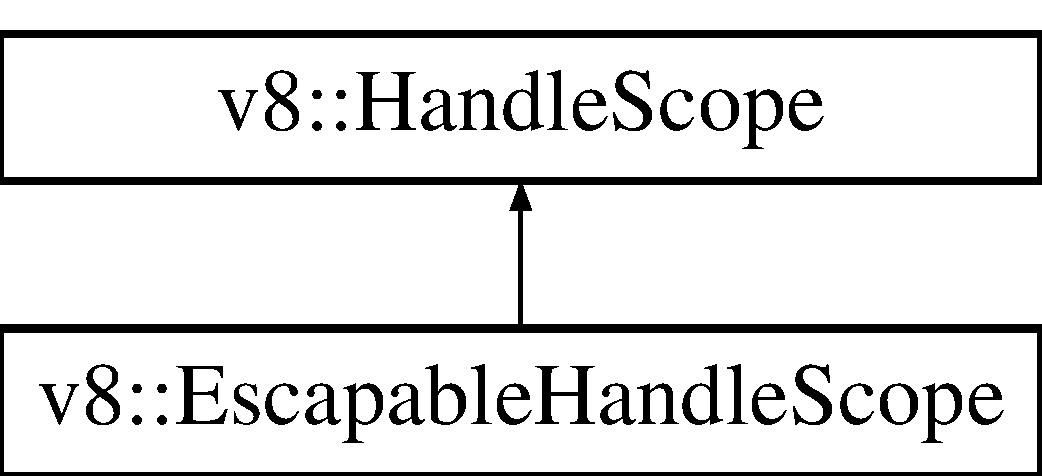
\includegraphics[height=2.000000cm]{classv8_1_1EscapableHandleScope}
\end{center}
\end{figure}
\subsection*{Public Member Functions}
\begin{DoxyCompactItemize}
\item 
{\bfseries Escapable\+Handle\+Scope} (\hyperlink{classv8_1_1Isolate}{Isolate} $\ast$isolate)\hypertarget{classv8_1_1EscapableHandleScope_aea39a7fd4dee6da31f3921ff891e1731}{}\label{classv8_1_1EscapableHandleScope_aea39a7fd4dee6da31f3921ff891e1731}

\item 
{\footnotesize template$<$class T $>$ }\\V8\+\_\+\+I\+N\+L\+I\+NE \hyperlink{classv8_1_1Local}{Local}$<$ T $>$ \hyperlink{classv8_1_1EscapableHandleScope_afdf0d3850978f65d1a827f78b3a2b6fd}{Escape} (\hyperlink{classv8_1_1Local}{Local}$<$ T $>$ value)
\end{DoxyCompactItemize}
\subsection*{Additional Inherited Members}


\subsection{Detailed Description}
A \hyperlink{classv8_1_1HandleScope}{Handle\+Scope} which first allocates a handle in the current scope which will be later filled with the escape value. 

\subsection{Member Function Documentation}
\index{v8\+::\+Escapable\+Handle\+Scope@{v8\+::\+Escapable\+Handle\+Scope}!Escape@{Escape}}
\index{Escape@{Escape}!v8\+::\+Escapable\+Handle\+Scope@{v8\+::\+Escapable\+Handle\+Scope}}
\subsubsection[{\texorpdfstring{Escape(\+Local$<$ T $>$ value)}{Escape(Local< T > value)}}]{\setlength{\rightskip}{0pt plus 5cm}template$<$class T $>$ V8\+\_\+\+I\+N\+L\+I\+NE {\bf Local}$<$T$>$ v8\+::\+Escapable\+Handle\+Scope\+::\+Escape (
\begin{DoxyParamCaption}
\item[{{\bf Local}$<$ T $>$}]{value}
\end{DoxyParamCaption}
)\hspace{0.3cm}{\ttfamily [inline]}}\hypertarget{classv8_1_1EscapableHandleScope_afdf0d3850978f65d1a827f78b3a2b6fd}{}\label{classv8_1_1EscapableHandleScope_afdf0d3850978f65d1a827f78b3a2b6fd}
Pushes the value into the previous scope and returns a handle to it. Cannot be called twice. 

The documentation for this class was generated from the following file\+:\begin{DoxyCompactItemize}
\item 
v8/include/v8.\+h\end{DoxyCompactItemize}

\hypertarget{classv8_1_1Eternal}{}\section{v8\+:\+:Eternal$<$ T $>$ Class Template Reference}
\label{classv8_1_1Eternal}\index{v8\+::\+Eternal$<$ T $>$@{v8\+::\+Eternal$<$ T $>$}}
\subsection*{Public Member Functions}
\begin{DoxyCompactItemize}
\item 
\hypertarget{classv8_1_1Eternal_ad7522d8b51e072dcbc4261bc1f155bcb}{}{\footnotesize template$<$class S $>$ }\\V8\+\_\+\+I\+N\+L\+I\+N\+E {\bfseries Eternal} (\hyperlink{classv8_1_1Isolate}{Isolate} $\ast$isolate, \hyperlink{classv8_1_1Local}{Local}$<$ S $>$ handle)\label{classv8_1_1Eternal_ad7522d8b51e072dcbc4261bc1f155bcb}

\item 
\hypertarget{classv8_1_1Eternal_ae9614309d9c93fe484d81926e31ed6b7}{}V8\+\_\+\+I\+N\+L\+I\+N\+E \hyperlink{classv8_1_1Local}{Local}$<$ T $>$ {\bfseries Get} (\hyperlink{classv8_1_1Isolate}{Isolate} $\ast$isolate)\label{classv8_1_1Eternal_ae9614309d9c93fe484d81926e31ed6b7}

\item 
\hypertarget{classv8_1_1Eternal_a5d77cbfe0662af5fe75172be9a8f1d5d}{}V8\+\_\+\+I\+N\+L\+I\+N\+E bool {\bfseries Is\+Empty} ()\label{classv8_1_1Eternal_a5d77cbfe0662af5fe75172be9a8f1d5d}

\item 
\hypertarget{classv8_1_1Eternal_a75a32f5c428a0d47e13f66dbdeb9adba}{}{\footnotesize template$<$class S $>$ }\\V8\+\_\+\+I\+N\+L\+I\+N\+E void {\bfseries Set} (\hyperlink{classv8_1_1Isolate}{Isolate} $\ast$isolate, \hyperlink{classv8_1_1Local}{Local}$<$ S $>$ handle)\label{classv8_1_1Eternal_a75a32f5c428a0d47e13f66dbdeb9adba}

\item 
\hypertarget{classv8_1_1Eternal_a2f9dcec02b2c2f7d4b55aee0d8b9881a}{}{\footnotesize template$<$class S $>$ }\\void {\bfseries Set} (\hyperlink{classv8_1_1Isolate}{Isolate} $\ast$isolate, \hyperlink{classv8_1_1Local}{Local}$<$ S $>$ handle)\label{classv8_1_1Eternal_a2f9dcec02b2c2f7d4b55aee0d8b9881a}

\end{DoxyCompactItemize}


The documentation for this class was generated from the following file\+:\begin{DoxyCompactItemize}
\item 
v8/include/v8.\+h\end{DoxyCompactItemize}

\hypertarget{classv8_1_1Debug_1_1EventDetails}{}\section{v8\+:\+:Debug\+:\+:Event\+Details Class Reference}
\label{classv8_1_1Debug_1_1EventDetails}\index{v8\+::\+Debug\+::\+Event\+Details@{v8\+::\+Debug\+::\+Event\+Details}}


{\ttfamily \#include $<$v8-\/debug.\+h$>$}

\subsection*{Public Member Functions}
\begin{DoxyCompactItemize}
\item 
virtual Debug\+Event \hyperlink{classv8_1_1Debug_1_1EventDetails_ac871568e8cfd43bbf2cdac62add34ed0}{Get\+Event} () const =0
\item 
virtual \hyperlink{classv8_1_1Local}{Local}$<$ \hyperlink{classv8_1_1Object}{Object} $>$ \hyperlink{classv8_1_1Debug_1_1EventDetails_a201fabdd6d81f711c1b8805c94f09d3e}{Get\+Execution\+State} () const =0
\item 
\hypertarget{classv8_1_1Debug_1_1EventDetails_a073451ff2ea6fc4c2acf46a6738aac69}{}virtual \hyperlink{classv8_1_1Local}{Local}$<$ \hyperlink{classv8_1_1Object}{Object} $>$ {\bfseries Get\+Event\+Data} () const =0\label{classv8_1_1Debug_1_1EventDetails_a073451ff2ea6fc4c2acf46a6738aac69}

\item 
virtual \hyperlink{classv8_1_1Local}{Local}$<$ \hyperlink{classv8_1_1Context}{Context} $>$ \hyperlink{classv8_1_1Debug_1_1EventDetails_aaa7573eeab71d8c4e914daeccddff77f}{Get\+Event\+Context} () const =0
\item 
virtual \hyperlink{classv8_1_1Local}{Local}$<$ \hyperlink{classv8_1_1Value}{Value} $>$ \hyperlink{classv8_1_1Debug_1_1EventDetails_aedd8014bb1bd644e227774d07ed9784d}{Get\+Callback\+Data} () const =0
\item 
virtual \hyperlink{classv8_1_1Debug_1_1ClientData}{Client\+Data} $\ast$ \hyperlink{classv8_1_1Debug_1_1EventDetails_ae663e7607d27c3252049eea077a83e08}{Get\+Client\+Data} () const =0
\end{DoxyCompactItemize}


\subsection{Detailed Description}
An event details object passed to the debug event listener. 

\subsection{Member Function Documentation}
\hypertarget{classv8_1_1Debug_1_1EventDetails_aedd8014bb1bd644e227774d07ed9784d}{}\index{v8\+::\+Debug\+::\+Event\+Details@{v8\+::\+Debug\+::\+Event\+Details}!Get\+Callback\+Data@{Get\+Callback\+Data}}
\index{Get\+Callback\+Data@{Get\+Callback\+Data}!v8\+::\+Debug\+::\+Event\+Details@{v8\+::\+Debug\+::\+Event\+Details}}
\subsubsection[{Get\+Callback\+Data}]{\setlength{\rightskip}{0pt plus 5cm}virtual {\bf Local}$<${\bf Value}$>$ v8\+::\+Debug\+::\+Event\+Details\+::\+Get\+Callback\+Data (
\begin{DoxyParamCaption}
{}
\end{DoxyParamCaption}
) const\hspace{0.3cm}{\ttfamily [pure virtual]}}\label{classv8_1_1Debug_1_1EventDetails_aedd8014bb1bd644e227774d07ed9784d}
Client data passed with the corresponding callback when it was registered. \hypertarget{classv8_1_1Debug_1_1EventDetails_ae663e7607d27c3252049eea077a83e08}{}\index{v8\+::\+Debug\+::\+Event\+Details@{v8\+::\+Debug\+::\+Event\+Details}!Get\+Client\+Data@{Get\+Client\+Data}}
\index{Get\+Client\+Data@{Get\+Client\+Data}!v8\+::\+Debug\+::\+Event\+Details@{v8\+::\+Debug\+::\+Event\+Details}}
\subsubsection[{Get\+Client\+Data}]{\setlength{\rightskip}{0pt plus 5cm}virtual {\bf Client\+Data}$\ast$ v8\+::\+Debug\+::\+Event\+Details\+::\+Get\+Client\+Data (
\begin{DoxyParamCaption}
{}
\end{DoxyParamCaption}
) const\hspace{0.3cm}{\ttfamily [pure virtual]}}\label{classv8_1_1Debug_1_1EventDetails_ae663e7607d27c3252049eea077a83e08}
Client data passed to Debug\+Break\+For\+Command function. The debugger takes ownership of the data and will delete it even if there is no message handler. \hypertarget{classv8_1_1Debug_1_1EventDetails_ac871568e8cfd43bbf2cdac62add34ed0}{}\index{v8\+::\+Debug\+::\+Event\+Details@{v8\+::\+Debug\+::\+Event\+Details}!Get\+Event@{Get\+Event}}
\index{Get\+Event@{Get\+Event}!v8\+::\+Debug\+::\+Event\+Details@{v8\+::\+Debug\+::\+Event\+Details}}
\subsubsection[{Get\+Event}]{\setlength{\rightskip}{0pt plus 5cm}virtual Debug\+Event v8\+::\+Debug\+::\+Event\+Details\+::\+Get\+Event (
\begin{DoxyParamCaption}
{}
\end{DoxyParamCaption}
) const\hspace{0.3cm}{\ttfamily [pure virtual]}}\label{classv8_1_1Debug_1_1EventDetails_ac871568e8cfd43bbf2cdac62add34ed0}
Event type. \hypertarget{classv8_1_1Debug_1_1EventDetails_aaa7573eeab71d8c4e914daeccddff77f}{}\index{v8\+::\+Debug\+::\+Event\+Details@{v8\+::\+Debug\+::\+Event\+Details}!Get\+Event\+Context@{Get\+Event\+Context}}
\index{Get\+Event\+Context@{Get\+Event\+Context}!v8\+::\+Debug\+::\+Event\+Details@{v8\+::\+Debug\+::\+Event\+Details}}
\subsubsection[{Get\+Event\+Context}]{\setlength{\rightskip}{0pt plus 5cm}virtual {\bf Local}$<${\bf Context}$>$ v8\+::\+Debug\+::\+Event\+Details\+::\+Get\+Event\+Context (
\begin{DoxyParamCaption}
{}
\end{DoxyParamCaption}
) const\hspace{0.3cm}{\ttfamily [pure virtual]}}\label{classv8_1_1Debug_1_1EventDetails_aaa7573eeab71d8c4e914daeccddff77f}
Get the context active when the debug event happened. Note this is not the current active context as the Java\+Script part of the debugger is running in its own context which is entered at this point. \hypertarget{classv8_1_1Debug_1_1EventDetails_a201fabdd6d81f711c1b8805c94f09d3e}{}\index{v8\+::\+Debug\+::\+Event\+Details@{v8\+::\+Debug\+::\+Event\+Details}!Get\+Execution\+State@{Get\+Execution\+State}}
\index{Get\+Execution\+State@{Get\+Execution\+State}!v8\+::\+Debug\+::\+Event\+Details@{v8\+::\+Debug\+::\+Event\+Details}}
\subsubsection[{Get\+Execution\+State}]{\setlength{\rightskip}{0pt plus 5cm}virtual {\bf Local}$<${\bf Object}$>$ v8\+::\+Debug\+::\+Event\+Details\+::\+Get\+Execution\+State (
\begin{DoxyParamCaption}
{}
\end{DoxyParamCaption}
) const\hspace{0.3cm}{\ttfamily [pure virtual]}}\label{classv8_1_1Debug_1_1EventDetails_a201fabdd6d81f711c1b8805c94f09d3e}
Access to execution state and event data of the debug event. Don\textquotesingle{}t store these cross callbacks as their content becomes invalid. 

The documentation for this class was generated from the following file\+:\begin{DoxyCompactItemize}
\item 
v8/include/v8-\/debug.\+h\end{DoxyCompactItemize}

\hypertarget{classv8_1_1Exception}{}\section{v8\+:\+:Exception Class Reference}
\label{classv8_1_1Exception}\index{v8\+::\+Exception@{v8\+::\+Exception}}


{\ttfamily \#include $<$v8.\+h$>$}

\subsection*{Static Public Member Functions}
\begin{DoxyCompactItemize}
\item 
\mbox{\Hypertarget{classv8_1_1Exception_a7fff335c54b4a267b5edab00ca049294}\label{classv8_1_1Exception_a7fff335c54b4a267b5edab00ca049294}} 
static \mbox{\hyperlink{classv8_1_1Local}{Local}}$<$ \mbox{\hyperlink{classv8_1_1Value}{Value}} $>$ {\bfseries Range\+Error} (\mbox{\hyperlink{classv8_1_1Local}{Local}}$<$ \mbox{\hyperlink{classv8_1_1String}{String}} $>$ message)
\item 
\mbox{\Hypertarget{classv8_1_1Exception_aa9a1b1806c6ec13e0e8852a05e83f8ef}\label{classv8_1_1Exception_aa9a1b1806c6ec13e0e8852a05e83f8ef}} 
static \mbox{\hyperlink{classv8_1_1Local}{Local}}$<$ \mbox{\hyperlink{classv8_1_1Value}{Value}} $>$ {\bfseries Reference\+Error} (\mbox{\hyperlink{classv8_1_1Local}{Local}}$<$ \mbox{\hyperlink{classv8_1_1String}{String}} $>$ message)
\item 
\mbox{\Hypertarget{classv8_1_1Exception_ae9efc01a15b3ea6ed0761ce4b2cfa4ab}\label{classv8_1_1Exception_ae9efc01a15b3ea6ed0761ce4b2cfa4ab}} 
static \mbox{\hyperlink{classv8_1_1Local}{Local}}$<$ \mbox{\hyperlink{classv8_1_1Value}{Value}} $>$ {\bfseries Syntax\+Error} (\mbox{\hyperlink{classv8_1_1Local}{Local}}$<$ \mbox{\hyperlink{classv8_1_1String}{String}} $>$ message)
\item 
\mbox{\Hypertarget{classv8_1_1Exception_ad06cda3370edb5b39a5c671bba28754d}\label{classv8_1_1Exception_ad06cda3370edb5b39a5c671bba28754d}} 
static \mbox{\hyperlink{classv8_1_1Local}{Local}}$<$ \mbox{\hyperlink{classv8_1_1Value}{Value}} $>$ {\bfseries Type\+Error} (\mbox{\hyperlink{classv8_1_1Local}{Local}}$<$ \mbox{\hyperlink{classv8_1_1String}{String}} $>$ message)
\item 
\mbox{\Hypertarget{classv8_1_1Exception_a77c6ab659f67df0cb0aa0f7c6698f019}\label{classv8_1_1Exception_a77c6ab659f67df0cb0aa0f7c6698f019}} 
static \mbox{\hyperlink{classv8_1_1Local}{Local}}$<$ \mbox{\hyperlink{classv8_1_1Value}{Value}} $>$ {\bfseries Error} (\mbox{\hyperlink{classv8_1_1Local}{Local}}$<$ \mbox{\hyperlink{classv8_1_1String}{String}} $>$ message)
\item 
static \mbox{\hyperlink{classv8_1_1Local}{Local}}$<$ \mbox{\hyperlink{classv8_1_1Message}{Message}} $>$ \mbox{\hyperlink{classv8_1_1Exception_a8d575a721cf0fd5b325afb8b586c0d1e}{Create\+Message}} (\mbox{\hyperlink{classv8_1_1Isolate}{Isolate}} $\ast$isolate, \mbox{\hyperlink{classv8_1_1Local}{Local}}$<$ \mbox{\hyperlink{classv8_1_1Value}{Value}} $>$ exception)
\item 
static \mbox{\hyperlink{classv8_1_1Local}{Local}}$<$ \mbox{\hyperlink{classv8_1_1StackTrace}{Stack\+Trace}} $>$ \mbox{\hyperlink{classv8_1_1Exception_a81d1fd3c8d729e9a8d830bc2830bfe77}{Get\+Stack\+Trace}} (\mbox{\hyperlink{classv8_1_1Local}{Local}}$<$ \mbox{\hyperlink{classv8_1_1Value}{Value}} $>$ exception)
\end{DoxyCompactItemize}


\subsection{Detailed Description}
Create new error objects by calling the corresponding error object constructor with the message. 

\subsection{Member Function Documentation}
\mbox{\Hypertarget{classv8_1_1Exception_a8d575a721cf0fd5b325afb8b586c0d1e}\label{classv8_1_1Exception_a8d575a721cf0fd5b325afb8b586c0d1e}} 
\index{v8\+::\+Exception@{v8\+::\+Exception}!Create\+Message@{Create\+Message}}
\index{Create\+Message@{Create\+Message}!v8\+::\+Exception@{v8\+::\+Exception}}
\subsubsection{\texorpdfstring{Create\+Message()}{CreateMessage()}}
{\footnotesize\ttfamily static \mbox{\hyperlink{classv8_1_1Local}{Local}}$<$\mbox{\hyperlink{classv8_1_1Message}{Message}}$>$ v8\+::\+Exception\+::\+Create\+Message (\begin{DoxyParamCaption}\item[{\mbox{\hyperlink{classv8_1_1Isolate}{Isolate}} $\ast$}]{isolate,  }\item[{\mbox{\hyperlink{classv8_1_1Local}{Local}}$<$ \mbox{\hyperlink{classv8_1_1Value}{Value}} $>$}]{exception }\end{DoxyParamCaption})\hspace{0.3cm}{\ttfamily [static]}}

Creates an error message for the given exception. Will try to reconstruct the original stack trace from the exception value, or capture the current stack trace if not available. \mbox{\Hypertarget{classv8_1_1Exception_a81d1fd3c8d729e9a8d830bc2830bfe77}\label{classv8_1_1Exception_a81d1fd3c8d729e9a8d830bc2830bfe77}} 
\index{v8\+::\+Exception@{v8\+::\+Exception}!Get\+Stack\+Trace@{Get\+Stack\+Trace}}
\index{Get\+Stack\+Trace@{Get\+Stack\+Trace}!v8\+::\+Exception@{v8\+::\+Exception}}
\subsubsection{\texorpdfstring{Get\+Stack\+Trace()}{GetStackTrace()}}
{\footnotesize\ttfamily static \mbox{\hyperlink{classv8_1_1Local}{Local}}$<$\mbox{\hyperlink{classv8_1_1StackTrace}{Stack\+Trace}}$>$ v8\+::\+Exception\+::\+Get\+Stack\+Trace (\begin{DoxyParamCaption}\item[{\mbox{\hyperlink{classv8_1_1Local}{Local}}$<$ \mbox{\hyperlink{classv8_1_1Value}{Value}} $>$}]{exception }\end{DoxyParamCaption})\hspace{0.3cm}{\ttfamily [static]}}

Returns the original stack trace that was captured at the creation time of a given exception, or an empty handle if not available. 

The documentation for this class was generated from the following file\+:\begin{DoxyCompactItemize}
\item 
v8/include/v8.\+h\end{DoxyCompactItemize}

\hypertarget{classv8_1_1Extension}{}\section{v8\+:\+:Extension Class Reference}
\label{classv8_1_1Extension}\index{v8\+::\+Extension@{v8\+::\+Extension}}


{\ttfamily \#include $<$v8.\+h$>$}

\subsection*{Public Member Functions}
\begin{DoxyCompactItemize}
\item 
\mbox{\Hypertarget{classv8_1_1Extension_a10868673b7801cc1139ca3bc09bcfcf6}\label{classv8_1_1Extension_a10868673b7801cc1139ca3bc09bcfcf6}} 
{\bfseries Extension} (const char $\ast$name, const char $\ast$source=0, int dep\+\_\+count=0, const char $\ast$$\ast$deps=0, int source\+\_\+length=-\/1)
\item 
\mbox{\Hypertarget{classv8_1_1Extension_ad19cfbd67437153672b65e048d672bb0}\label{classv8_1_1Extension_ad19cfbd67437153672b65e048d672bb0}} 
virtual \mbox{\hyperlink{classv8_1_1Local}{Local}}$<$ \mbox{\hyperlink{classv8_1_1FunctionTemplate}{Function\+Template}} $>$ {\bfseries Get\+Native\+Function\+Template} (\mbox{\hyperlink{classv8_1_1Isolate}{Isolate}} $\ast$isolate, \mbox{\hyperlink{classv8_1_1Local}{Local}}$<$ \mbox{\hyperlink{classv8_1_1String}{String}} $>$ name)
\item 
\mbox{\Hypertarget{classv8_1_1Extension_a2aa7793ae4322dd8c1f15362e4b13244}\label{classv8_1_1Extension_a2aa7793ae4322dd8c1f15362e4b13244}} 
const char $\ast$ {\bfseries name} () const
\item 
\mbox{\Hypertarget{classv8_1_1Extension_a61a481f21654fc3d8007453dc7ef92e3}\label{classv8_1_1Extension_a61a481f21654fc3d8007453dc7ef92e3}} 
size\+\_\+t {\bfseries source\+\_\+length} () const
\item 
\mbox{\Hypertarget{classv8_1_1Extension_a5ffec9002da1eb1390a06ca02fcfcc0a}\label{classv8_1_1Extension_a5ffec9002da1eb1390a06ca02fcfcc0a}} 
const \mbox{\hyperlink{classv8_1_1String_1_1ExternalOneByteStringResource}{String\+::\+External\+One\+Byte\+String\+Resource}} $\ast$ {\bfseries source} () const
\item 
\mbox{\Hypertarget{classv8_1_1Extension_a7623b08e3bc42d903bd923a00317b7f9}\label{classv8_1_1Extension_a7623b08e3bc42d903bd923a00317b7f9}} 
int {\bfseries dependency\+\_\+count} ()
\item 
\mbox{\Hypertarget{classv8_1_1Extension_adbec8a811d5a4554678da4a5d55dda6d}\label{classv8_1_1Extension_adbec8a811d5a4554678da4a5d55dda6d}} 
const char $\ast$$\ast$ {\bfseries dependencies} ()
\item 
\mbox{\Hypertarget{classv8_1_1Extension_af5b752ba211315b6e9dac5c0e6e638e8}\label{classv8_1_1Extension_af5b752ba211315b6e9dac5c0e6e638e8}} 
void {\bfseries set\+\_\+auto\+\_\+enable} (bool value)
\item 
\mbox{\Hypertarget{classv8_1_1Extension_aee87ef4f9c3d7880fc3b28765d28e516}\label{classv8_1_1Extension_aee87ef4f9c3d7880fc3b28765d28e516}} 
bool {\bfseries auto\+\_\+enable} ()
\item 
\mbox{\Hypertarget{classv8_1_1Extension_a653667ad2af68a5969f5f64c9f765e73}\label{classv8_1_1Extension_a653667ad2af68a5969f5f64c9f765e73}} 
{\bfseries Extension} (const \mbox{\hyperlink{classv8_1_1Extension}{Extension}} \&)=delete
\item 
\mbox{\Hypertarget{classv8_1_1Extension_a9534122f8ad68e5a1e3dd8a9f5c5311a}\label{classv8_1_1Extension_a9534122f8ad68e5a1e3dd8a9f5c5311a}} 
void {\bfseries operator=} (const \mbox{\hyperlink{classv8_1_1Extension}{Extension}} \&)=delete
\end{DoxyCompactItemize}


\subsection{Detailed Description}
Ignore 

The documentation for this class was generated from the following file\+:\begin{DoxyCompactItemize}
\item 
v8/include/v8.\+h\end{DoxyCompactItemize}

\hypertarget{classv8_1_1ExtensionConfiguration}{\section{v8\-:\-:Extension\-Configuration Class Reference}
\label{classv8_1_1ExtensionConfiguration}\index{v8\-::\-Extension\-Configuration@{v8\-::\-Extension\-Configuration}}
}


{\ttfamily \#include $<$v8.\-h$>$}

\subsection*{Public Member Functions}
\begin{DoxyCompactItemize}
\item 
\hypertarget{classv8_1_1ExtensionConfiguration_a1189e46efe963db4aa7340cc767f276a}{{\bfseries Extension\-Configuration} (int name\-\_\-count, const char $\ast$names\mbox{[}$\,$\mbox{]})}\label{classv8_1_1ExtensionConfiguration_a1189e46efe963db4aa7340cc767f276a}

\item 
\hypertarget{classv8_1_1ExtensionConfiguration_ae776fbc067a257bac854d9bcc9b72141}{const char $\ast$$\ast$ {\bfseries begin} () const }\label{classv8_1_1ExtensionConfiguration_ae776fbc067a257bac854d9bcc9b72141}

\item 
\hypertarget{classv8_1_1ExtensionConfiguration_abcbebcc4782016f58fc60de82f59f61a}{const char $\ast$$\ast$ {\bfseries end} () const }\label{classv8_1_1ExtensionConfiguration_abcbebcc4782016f58fc60de82f59f61a}

\end{DoxyCompactItemize}


\subsection{Detailed Description}
A container for extension names. 

The documentation for this class was generated from the following file\-:\begin{DoxyCompactItemize}
\item 
v8/include/v8.\-h\end{DoxyCompactItemize}

\hypertarget{classv8_1_1External}{}\section{v8\+:\+:External Class Reference}
\label{classv8_1_1External}\index{v8\+::\+External@{v8\+::\+External}}


{\ttfamily \#include $<$v8.\+h$>$}

Inheritance diagram for v8\+:\+:External\+:\begin{figure}[H]
\begin{center}
\leavevmode
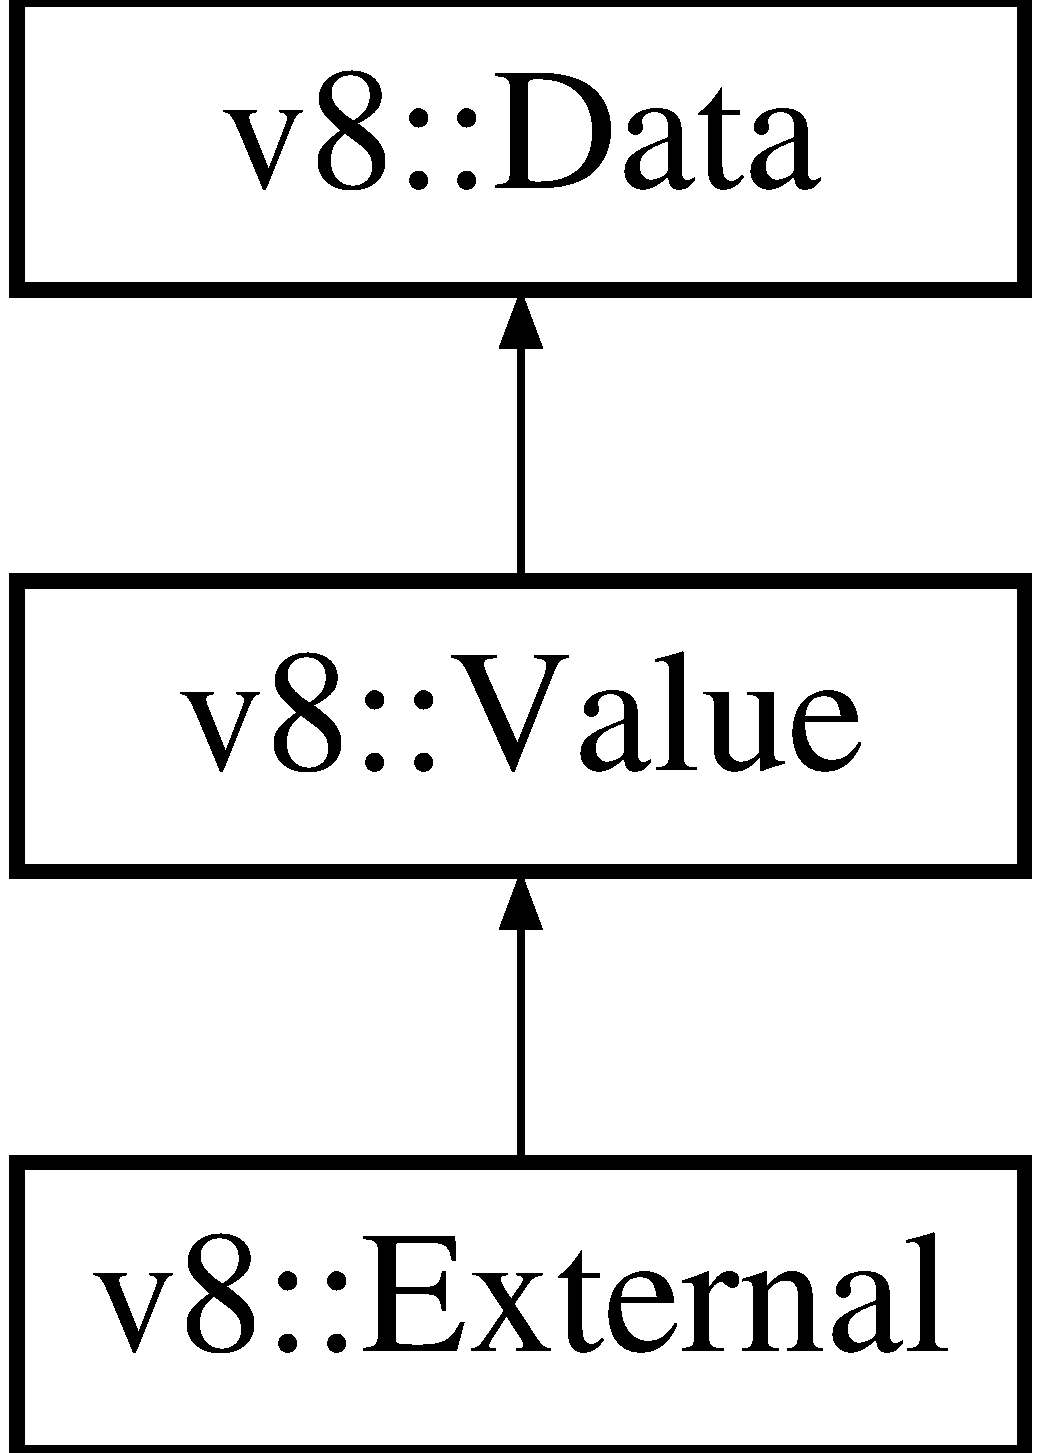
\includegraphics[height=3.000000cm]{classv8_1_1External}
\end{center}
\end{figure}
\subsection*{Public Member Functions}
\begin{DoxyCompactItemize}
\item 
\mbox{\Hypertarget{classv8_1_1External_a5d5f967787189f6e2e35c51836862777}\label{classv8_1_1External_a5d5f967787189f6e2e35c51836862777}} 
void $\ast$ {\bfseries Value} () const
\end{DoxyCompactItemize}
\subsection*{Static Public Member Functions}
\begin{DoxyCompactItemize}
\item 
\mbox{\Hypertarget{classv8_1_1External_a1e877f692e95f13ac3102707ce8cbab9}\label{classv8_1_1External_a1e877f692e95f13ac3102707ce8cbab9}} 
static \mbox{\hyperlink{classv8_1_1Local}{Local}}$<$ \mbox{\hyperlink{classv8_1_1External}{External}} $>$ {\bfseries New} (Isolate $\ast$isolate, void $\ast$value)
\item 
\mbox{\Hypertarget{classv8_1_1External_a4711aba26710c5dd72f11cb81808f9c2}\label{classv8_1_1External_a4711aba26710c5dd72f11cb81808f9c2}} 
static V8\+\_\+\+I\+N\+L\+I\+NE \mbox{\hyperlink{classv8_1_1External}{External}} $\ast$ {\bfseries Cast} (\mbox{\hyperlink{classv8_1_1Value}{Value}} $\ast$obj)
\end{DoxyCompactItemize}


\subsection{Detailed Description}
A Java\+Script value that wraps a C++ void$\ast$. This type of value is mainly used to associate C++ data structures with Java\+Script objects. 

Definition at line 5257 of file v8.\+h.



The documentation for this class was generated from the following file\+:\begin{DoxyCompactItemize}
\item 
v8/include/v8.\+h\end{DoxyCompactItemize}

\hypertarget{classv8_1_1String_1_1ExternalOneByteStringResource}{}\section{v8\+:\+:String\+:\+:External\+One\+Byte\+String\+Resource Class Reference}
\label{classv8_1_1String_1_1ExternalOneByteStringResource}\index{v8\+::\+String\+::\+External\+One\+Byte\+String\+Resource@{v8\+::\+String\+::\+External\+One\+Byte\+String\+Resource}}


{\ttfamily \#include $<$v8.\+h$>$}

Inheritance diagram for v8\+:\+:String\+:\+:External\+One\+Byte\+String\+Resource\+:\begin{figure}[H]
\begin{center}
\leavevmode
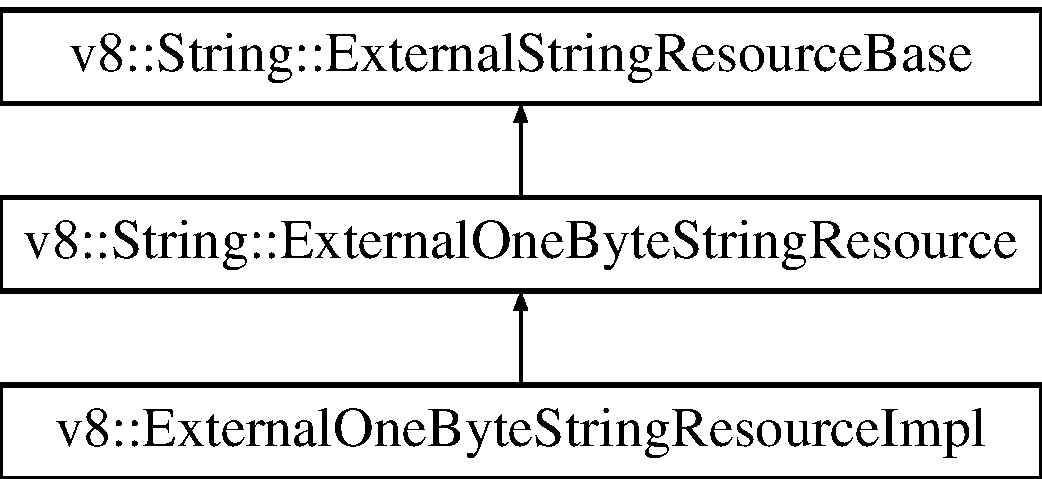
\includegraphics[height=2.000000cm]{classv8_1_1String_1_1ExternalOneByteStringResource}
\end{center}
\end{figure}
\subsection*{Public Member Functions}
\begin{DoxyCompactItemize}
\item 
\mbox{\hyperlink{classv8_1_1String_1_1ExternalOneByteStringResource_ac75c47722e5602b863cbc880dc4f5b7c}{$\sim$\+External\+One\+Byte\+String\+Resource}} () override=default
\item 
virtual const char $\ast$ \mbox{\hyperlink{classv8_1_1String_1_1ExternalOneByteStringResource_aaeca31240d3dbf990d1b974e3c64593e}{data}} () const =0
\item 
virtual size\+\_\+t \mbox{\hyperlink{classv8_1_1String_1_1ExternalOneByteStringResource_ad6b702f05798bcfc3975cb922f32b5ab}{length}} () const =0
\end{DoxyCompactItemize}
\subsection*{Additional Inherited Members}


\subsection{Detailed Description}
An \mbox{\hyperlink{classv8_1_1String_1_1ExternalOneByteStringResource}{External\+One\+Byte\+String\+Resource}} is a wrapper around an one-\/byte string buffer that resides outside V8\textquotesingle{}s heap. Implement an \mbox{\hyperlink{classv8_1_1String_1_1ExternalOneByteStringResource}{External\+One\+Byte\+String\+Resource}} to manage the life cycle of the underlying buffer. Note that the string data must be immutable and that the data must be Latin-\/1 and not U\+T\+F-\/8, which would require special treatment internally in the engine and do not allow efficient indexing. Use String\+::\+New or convert to 16 bit data for non-\/\+Latin1. 

\subsection{Constructor \& Destructor Documentation}
\mbox{\Hypertarget{classv8_1_1String_1_1ExternalOneByteStringResource_ac75c47722e5602b863cbc880dc4f5b7c}\label{classv8_1_1String_1_1ExternalOneByteStringResource_ac75c47722e5602b863cbc880dc4f5b7c}} 
\index{v8\+::\+String\+::\+External\+One\+Byte\+String\+Resource@{v8\+::\+String\+::\+External\+One\+Byte\+String\+Resource}!````~External\+One\+Byte\+String\+Resource@{$\sim$\+External\+One\+Byte\+String\+Resource}}
\index{````~External\+One\+Byte\+String\+Resource@{$\sim$\+External\+One\+Byte\+String\+Resource}!v8\+::\+String\+::\+External\+One\+Byte\+String\+Resource@{v8\+::\+String\+::\+External\+One\+Byte\+String\+Resource}}
\subsubsection{\texorpdfstring{$\sim$\+External\+One\+Byte\+String\+Resource()}{~ExternalOneByteStringResource()}}
{\footnotesize\ttfamily v8\+::\+String\+::\+External\+One\+Byte\+String\+Resource\+::$\sim$\+External\+One\+Byte\+String\+Resource (\begin{DoxyParamCaption}{ }\end{DoxyParamCaption})\hspace{0.3cm}{\ttfamily [override]}, {\ttfamily [default]}}

Override the destructor to manage the life cycle of the underlying buffer. 

\subsection{Member Function Documentation}
\mbox{\Hypertarget{classv8_1_1String_1_1ExternalOneByteStringResource_aaeca31240d3dbf990d1b974e3c64593e}\label{classv8_1_1String_1_1ExternalOneByteStringResource_aaeca31240d3dbf990d1b974e3c64593e}} 
\index{v8\+::\+String\+::\+External\+One\+Byte\+String\+Resource@{v8\+::\+String\+::\+External\+One\+Byte\+String\+Resource}!data@{data}}
\index{data@{data}!v8\+::\+String\+::\+External\+One\+Byte\+String\+Resource@{v8\+::\+String\+::\+External\+One\+Byte\+String\+Resource}}
\subsubsection{\texorpdfstring{data()}{data()}}
{\footnotesize\ttfamily virtual const char$\ast$ v8\+::\+String\+::\+External\+One\+Byte\+String\+Resource\+::data (\begin{DoxyParamCaption}{ }\end{DoxyParamCaption}) const\hspace{0.3cm}{\ttfamily [pure virtual]}}

The string data from the underlying buffer. \mbox{\Hypertarget{classv8_1_1String_1_1ExternalOneByteStringResource_ad6b702f05798bcfc3975cb922f32b5ab}\label{classv8_1_1String_1_1ExternalOneByteStringResource_ad6b702f05798bcfc3975cb922f32b5ab}} 
\index{v8\+::\+String\+::\+External\+One\+Byte\+String\+Resource@{v8\+::\+String\+::\+External\+One\+Byte\+String\+Resource}!length@{length}}
\index{length@{length}!v8\+::\+String\+::\+External\+One\+Byte\+String\+Resource@{v8\+::\+String\+::\+External\+One\+Byte\+String\+Resource}}
\subsubsection{\texorpdfstring{length()}{length()}}
{\footnotesize\ttfamily virtual size\+\_\+t v8\+::\+String\+::\+External\+One\+Byte\+String\+Resource\+::length (\begin{DoxyParamCaption}{ }\end{DoxyParamCaption}) const\hspace{0.3cm}{\ttfamily [pure virtual]}}

The number of Latin-\/1 characters in the string. 

The documentation for this class was generated from the following file\+:\begin{DoxyCompactItemize}
\item 
v8/include/v8.\+h\end{DoxyCompactItemize}

\hypertarget{classv8_1_1ExternalOneByteStringResourceImpl}{}\section{v8\+:\+:External\+One\+Byte\+String\+Resource\+Impl Class Reference}
\label{classv8_1_1ExternalOneByteStringResourceImpl}\index{v8\+::\+External\+One\+Byte\+String\+Resource\+Impl@{v8\+::\+External\+One\+Byte\+String\+Resource\+Impl}}
Inheritance diagram for v8\+:\+:External\+One\+Byte\+String\+Resource\+Impl\+:\begin{figure}[H]
\begin{center}
\leavevmode
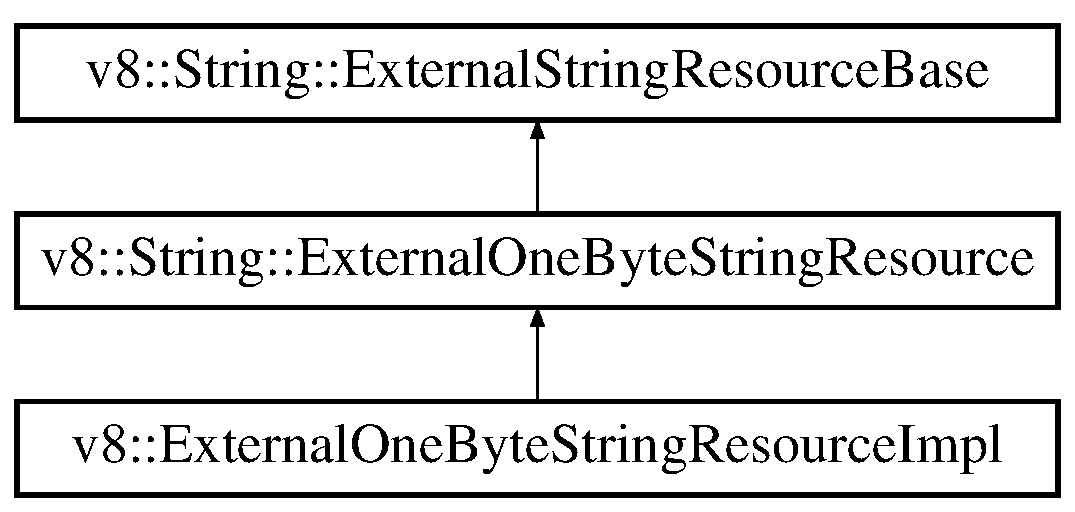
\includegraphics[height=3.000000cm]{classv8_1_1ExternalOneByteStringResourceImpl}
\end{center}
\end{figure}
\subsection*{Public Member Functions}
\begin{DoxyCompactItemize}
\item 
\hypertarget{classv8_1_1ExternalOneByteStringResourceImpl_a46178fb208419f5ea99552871b3a373e}{}{\bfseries External\+One\+Byte\+String\+Resource\+Impl} (const char $\ast$\hyperlink{classv8_1_1ExternalOneByteStringResourceImpl_a37ada5dc21ecb982c50482c90fffe529}{data}, size\+\_\+t \hyperlink{classv8_1_1ExternalOneByteStringResourceImpl_aedcf350d46f64cf1e3045658920d1dc8}{length})\label{classv8_1_1ExternalOneByteStringResourceImpl_a46178fb208419f5ea99552871b3a373e}

\item 
const char $\ast$ \hyperlink{classv8_1_1ExternalOneByteStringResourceImpl_a37ada5dc21ecb982c50482c90fffe529}{data} () const 
\item 
size\+\_\+t \hyperlink{classv8_1_1ExternalOneByteStringResourceImpl_aedcf350d46f64cf1e3045658920d1dc8}{length} () const 
\end{DoxyCompactItemize}
\subsection*{Additional Inherited Members}


\subsection{Member Function Documentation}
\hypertarget{classv8_1_1ExternalOneByteStringResourceImpl_a37ada5dc21ecb982c50482c90fffe529}{}\index{v8\+::\+External\+One\+Byte\+String\+Resource\+Impl@{v8\+::\+External\+One\+Byte\+String\+Resource\+Impl}!data@{data}}
\index{data@{data}!v8\+::\+External\+One\+Byte\+String\+Resource\+Impl@{v8\+::\+External\+One\+Byte\+String\+Resource\+Impl}}
\subsubsection[{data}]{\setlength{\rightskip}{0pt plus 5cm}const char$\ast$ v8\+::\+External\+One\+Byte\+String\+Resource\+Impl\+::data (
\begin{DoxyParamCaption}
{}
\end{DoxyParamCaption}
) const\hspace{0.3cm}{\ttfamily [inline]}, {\ttfamily [virtual]}}\label{classv8_1_1ExternalOneByteStringResourceImpl_a37ada5dc21ecb982c50482c90fffe529}
The string data from the underlying buffer. 

Implements \hyperlink{classv8_1_1String_1_1ExternalOneByteStringResource_aaeca31240d3dbf990d1b974e3c64593e}{v8\+::\+String\+::\+External\+One\+Byte\+String\+Resource}.

\hypertarget{classv8_1_1ExternalOneByteStringResourceImpl_aedcf350d46f64cf1e3045658920d1dc8}{}\index{v8\+::\+External\+One\+Byte\+String\+Resource\+Impl@{v8\+::\+External\+One\+Byte\+String\+Resource\+Impl}!length@{length}}
\index{length@{length}!v8\+::\+External\+One\+Byte\+String\+Resource\+Impl@{v8\+::\+External\+One\+Byte\+String\+Resource\+Impl}}
\subsubsection[{length}]{\setlength{\rightskip}{0pt plus 5cm}size\+\_\+t v8\+::\+External\+One\+Byte\+String\+Resource\+Impl\+::length (
\begin{DoxyParamCaption}
{}
\end{DoxyParamCaption}
) const\hspace{0.3cm}{\ttfamily [inline]}, {\ttfamily [virtual]}}\label{classv8_1_1ExternalOneByteStringResourceImpl_aedcf350d46f64cf1e3045658920d1dc8}
The number of Latin-\/1 characters in the string. 

Implements \hyperlink{classv8_1_1String_1_1ExternalOneByteStringResource_ad6b702f05798bcfc3975cb922f32b5ab}{v8\+::\+String\+::\+External\+One\+Byte\+String\+Resource}.



The documentation for this class was generated from the following file\+:\begin{DoxyCompactItemize}
\item 
v8/include/v8.\+h\end{DoxyCompactItemize}

\hypertarget{classv8_1_1ExternalResourceVisitor}{}\section{v8\+:\+:External\+Resource\+Visitor Class Reference}
\label{classv8_1_1ExternalResourceVisitor}\index{v8\+::\+External\+Resource\+Visitor@{v8\+::\+External\+Resource\+Visitor}}


{\ttfamily \#include $<$v8.\+h$>$}

\subsection*{Public Member Functions}
\begin{DoxyCompactItemize}
\item 
virtual void {\bfseries Visit\+External\+String} (\hyperlink{classv8_1_1Local}{Local}$<$ \hyperlink{classv8_1_1String}{String} $>$ string)\hypertarget{classv8_1_1ExternalResourceVisitor_ad611b1b6a06753f8eaf6936f793441bd}{}\label{classv8_1_1ExternalResourceVisitor_ad611b1b6a06753f8eaf6936f793441bd}

\end{DoxyCompactItemize}


\subsection{Detailed Description}
Interface for iterating through all external resources in the heap. 

The documentation for this class was generated from the following file\+:\begin{DoxyCompactItemize}
\item 
v8/include/v8.\+h\end{DoxyCompactItemize}

\hypertarget{classv8_1_1ScriptCompiler_1_1ExternalSourceStream}{}\section{v8\+:\+:Script\+Compiler\+:\+:External\+Source\+Stream Class Reference}
\label{classv8_1_1ScriptCompiler_1_1ExternalSourceStream}\index{v8\+::\+Script\+Compiler\+::\+External\+Source\+Stream@{v8\+::\+Script\+Compiler\+::\+External\+Source\+Stream}}


{\ttfamily \#include $<$v8.\+h$>$}

\subsection*{Public Member Functions}
\begin{DoxyCompactItemize}
\item 
virtual size\+\_\+t \mbox{\hyperlink{classv8_1_1ScriptCompiler_1_1ExternalSourceStream_ac3a0221b5725f0b612a6342d8e83d899}{Get\+More\+Data}} (const uint8\+\_\+t $\ast$$\ast$src)=0
\item 
virtual bool \mbox{\hyperlink{classv8_1_1ScriptCompiler_1_1ExternalSourceStream_a6848508547b3508a2d016738f12561e8}{Set\+Bookmark}} ()
\item 
virtual void \mbox{\hyperlink{classv8_1_1ScriptCompiler_1_1ExternalSourceStream_a425cf1ba265eeca194b805fe5c52bc19}{Reset\+To\+Bookmark}} ()
\end{DoxyCompactItemize}


\subsection{Detailed Description}
For streaming incomplete script data to \mbox{\hyperlink{classv8_1_1V8}{V8}}. The embedder should implement a subclass of this class. 

\subsection{Member Function Documentation}
\mbox{\Hypertarget{classv8_1_1ScriptCompiler_1_1ExternalSourceStream_ac3a0221b5725f0b612a6342d8e83d899}\label{classv8_1_1ScriptCompiler_1_1ExternalSourceStream_ac3a0221b5725f0b612a6342d8e83d899}} 
\index{v8\+::\+Script\+Compiler\+::\+External\+Source\+Stream@{v8\+::\+Script\+Compiler\+::\+External\+Source\+Stream}!Get\+More\+Data@{Get\+More\+Data}}
\index{Get\+More\+Data@{Get\+More\+Data}!v8\+::\+Script\+Compiler\+::\+External\+Source\+Stream@{v8\+::\+Script\+Compiler\+::\+External\+Source\+Stream}}
\subsubsection{\texorpdfstring{Get\+More\+Data()}{GetMoreData()}}
{\footnotesize\ttfamily virtual size\+\_\+t v8\+::\+Script\+Compiler\+::\+External\+Source\+Stream\+::\+Get\+More\+Data (\begin{DoxyParamCaption}\item[{const uint8\+\_\+t $\ast$$\ast$}]{src }\end{DoxyParamCaption})\hspace{0.3cm}{\ttfamily [pure virtual]}}

\mbox{\hyperlink{classv8_1_1V8}{V8}} calls this to request the next chunk of data from the embedder. This function will be called on a background thread, so it\textquotesingle{}s OK to block and wait for the data, if the embedder doesn\textquotesingle{}t have data yet. Returns the length of the data returned. When the data ends, Get\+More\+Data should return 0. Caller takes ownership of the data.

When streaming U\+T\+F-\/8 data, \mbox{\hyperlink{classv8_1_1V8}{V8}} handles multi-\/byte characters split between two data chunks, but doesn\textquotesingle{}t handle multi-\/byte characters split between more than two data chunks. The embedder can avoid this problem by always returning at least 2 bytes of data.

When streaming U\+T\+F-\/16 data, \mbox{\hyperlink{classv8_1_1V8}{V8}} does not handle characters split between two data chunks. The embedder has to make sure that chunks have an even length.

If the embedder wants to cancel the streaming, they should make the next Get\+More\+Data call return 0. \mbox{\hyperlink{classv8_1_1V8}{V8}} will interpret it as end of data (and most probably, parsing will fail). The streaming task will return as soon as \mbox{\hyperlink{classv8_1_1V8}{V8}} has parsed the data it received so far. \mbox{\Hypertarget{classv8_1_1ScriptCompiler_1_1ExternalSourceStream_a425cf1ba265eeca194b805fe5c52bc19}\label{classv8_1_1ScriptCompiler_1_1ExternalSourceStream_a425cf1ba265eeca194b805fe5c52bc19}} 
\index{v8\+::\+Script\+Compiler\+::\+External\+Source\+Stream@{v8\+::\+Script\+Compiler\+::\+External\+Source\+Stream}!Reset\+To\+Bookmark@{Reset\+To\+Bookmark}}
\index{Reset\+To\+Bookmark@{Reset\+To\+Bookmark}!v8\+::\+Script\+Compiler\+::\+External\+Source\+Stream@{v8\+::\+Script\+Compiler\+::\+External\+Source\+Stream}}
\subsubsection{\texorpdfstring{Reset\+To\+Bookmark()}{ResetToBookmark()}}
{\footnotesize\ttfamily virtual void v8\+::\+Script\+Compiler\+::\+External\+Source\+Stream\+::\+Reset\+To\+Bookmark (\begin{DoxyParamCaption}{ }\end{DoxyParamCaption})\hspace{0.3cm}{\ttfamily [virtual]}}

\mbox{\hyperlink{classv8_1_1V8}{V8}} calls this to return to a previously set bookmark. \mbox{\Hypertarget{classv8_1_1ScriptCompiler_1_1ExternalSourceStream_a6848508547b3508a2d016738f12561e8}\label{classv8_1_1ScriptCompiler_1_1ExternalSourceStream_a6848508547b3508a2d016738f12561e8}} 
\index{v8\+::\+Script\+Compiler\+::\+External\+Source\+Stream@{v8\+::\+Script\+Compiler\+::\+External\+Source\+Stream}!Set\+Bookmark@{Set\+Bookmark}}
\index{Set\+Bookmark@{Set\+Bookmark}!v8\+::\+Script\+Compiler\+::\+External\+Source\+Stream@{v8\+::\+Script\+Compiler\+::\+External\+Source\+Stream}}
\subsubsection{\texorpdfstring{Set\+Bookmark()}{SetBookmark()}}
{\footnotesize\ttfamily virtual bool v8\+::\+Script\+Compiler\+::\+External\+Source\+Stream\+::\+Set\+Bookmark (\begin{DoxyParamCaption}{ }\end{DoxyParamCaption})\hspace{0.3cm}{\ttfamily [virtual]}}

\mbox{\hyperlink{classv8_1_1V8}{V8}} calls this method to set a \textquotesingle{}bookmark\textquotesingle{} at the current position in the source stream, for the purpose of (maybe) later calling Reset\+To\+Bookmark. If Reset\+To\+Bookmark is called later, then subsequent calls to Get\+More\+Data should return the same data as they did when Set\+Bookmark was called earlier.

The embedder may return \textquotesingle{}false\textquotesingle{} to indicate it cannot provide this functionality. 

The documentation for this class was generated from the following file\+:\begin{DoxyCompactItemize}
\item 
v8/include/v8.\+h\end{DoxyCompactItemize}

\hypertarget{classv8_1_1String_1_1ExternalStringResource}{}\section{v8\+:\+:String\+:\+:External\+String\+Resource Class Reference}
\label{classv8_1_1String_1_1ExternalStringResource}\index{v8\+::\+String\+::\+External\+String\+Resource@{v8\+::\+String\+::\+External\+String\+Resource}}


{\ttfamily \#include $<$v8.\+h$>$}

Inheritance diagram for v8\+:\+:String\+:\+:External\+String\+Resource\+:\begin{figure}[H]
\begin{center}
\leavevmode
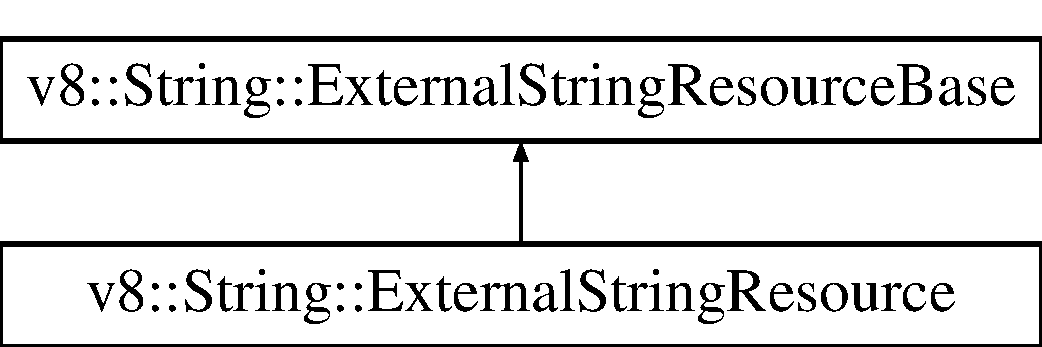
\includegraphics[height=2.000000cm]{classv8_1_1String_1_1ExternalStringResource}
\end{center}
\end{figure}
\subsection*{Public Member Functions}
\begin{DoxyCompactItemize}
\item 
\mbox{\hyperlink{classv8_1_1String_1_1ExternalStringResource_ad5f8c0ca1ed53d7c1ec7b11dc0aef49c}{$\sim$\+External\+String\+Resource}} () override=default
\item 
virtual const uint16\+\_\+t $\ast$ \mbox{\hyperlink{classv8_1_1String_1_1ExternalStringResource_a987309199b848511adb708e221e0fb0a}{data}} () const =0
\item 
virtual size\+\_\+t \mbox{\hyperlink{classv8_1_1String_1_1ExternalStringResource_ab5ca300fea077d7c7774ec49d32e4da1}{length}} () const =0
\end{DoxyCompactItemize}
\subsection*{Additional Inherited Members}


\subsection{Detailed Description}
An \mbox{\hyperlink{classv8_1_1String_1_1ExternalStringResource}{External\+String\+Resource}} is a wrapper around a two-\/byte string buffer that resides outside V8\textquotesingle{}s heap. Implement an \mbox{\hyperlink{classv8_1_1String_1_1ExternalStringResource}{External\+String\+Resource}} to manage the life cycle of the underlying buffer. Note that the string data must be immutable. 

Definition at line 2695 of file v8.\+h.



\subsection{Constructor \& Destructor Documentation}
\mbox{\Hypertarget{classv8_1_1String_1_1ExternalStringResource_ad5f8c0ca1ed53d7c1ec7b11dc0aef49c}\label{classv8_1_1String_1_1ExternalStringResource_ad5f8c0ca1ed53d7c1ec7b11dc0aef49c}} 
\index{v8\+::\+String\+::\+External\+String\+Resource@{v8\+::\+String\+::\+External\+String\+Resource}!````~External\+String\+Resource@{$\sim$\+External\+String\+Resource}}
\index{````~External\+String\+Resource@{$\sim$\+External\+String\+Resource}!v8\+::\+String\+::\+External\+String\+Resource@{v8\+::\+String\+::\+External\+String\+Resource}}
\subsubsection{\texorpdfstring{$\sim$\+External\+String\+Resource()}{~ExternalStringResource()}}
{\footnotesize\ttfamily v8\+::\+String\+::\+External\+String\+Resource\+::$\sim$\+External\+String\+Resource (\begin{DoxyParamCaption}{ }\end{DoxyParamCaption})\hspace{0.3cm}{\ttfamily [override]}, {\ttfamily [default]}}

Override the destructor to manage the life cycle of the underlying buffer. 

\subsection{Member Function Documentation}
\mbox{\Hypertarget{classv8_1_1String_1_1ExternalStringResource_a987309199b848511adb708e221e0fb0a}\label{classv8_1_1String_1_1ExternalStringResource_a987309199b848511adb708e221e0fb0a}} 
\index{v8\+::\+String\+::\+External\+String\+Resource@{v8\+::\+String\+::\+External\+String\+Resource}!data@{data}}
\index{data@{data}!v8\+::\+String\+::\+External\+String\+Resource@{v8\+::\+String\+::\+External\+String\+Resource}}
\subsubsection{\texorpdfstring{data()}{data()}}
{\footnotesize\ttfamily virtual const uint16\+\_\+t$\ast$ v8\+::\+String\+::\+External\+String\+Resource\+::data (\begin{DoxyParamCaption}{ }\end{DoxyParamCaption}) const\hspace{0.3cm}{\ttfamily [pure virtual]}}

The string data from the underlying buffer. \mbox{\Hypertarget{classv8_1_1String_1_1ExternalStringResource_ab5ca300fea077d7c7774ec49d32e4da1}\label{classv8_1_1String_1_1ExternalStringResource_ab5ca300fea077d7c7774ec49d32e4da1}} 
\index{v8\+::\+String\+::\+External\+String\+Resource@{v8\+::\+String\+::\+External\+String\+Resource}!length@{length}}
\index{length@{length}!v8\+::\+String\+::\+External\+String\+Resource@{v8\+::\+String\+::\+External\+String\+Resource}}
\subsubsection{\texorpdfstring{length()}{length()}}
{\footnotesize\ttfamily virtual size\+\_\+t v8\+::\+String\+::\+External\+String\+Resource\+::length (\begin{DoxyParamCaption}{ }\end{DoxyParamCaption}) const\hspace{0.3cm}{\ttfamily [pure virtual]}}

The length of the string. That is, the number of two-\/byte characters. 

The documentation for this class was generated from the following file\+:\begin{DoxyCompactItemize}
\item 
v8/include/v8.\+h\end{DoxyCompactItemize}

\hypertarget{classv8_1_1String_1_1ExternalStringResourceBase}{}\section{v8\+:\+:String\+:\+:External\+String\+Resource\+Base Class Reference}
\label{classv8_1_1String_1_1ExternalStringResourceBase}\index{v8\+::\+String\+::\+External\+String\+Resource\+Base@{v8\+::\+String\+::\+External\+String\+Resource\+Base}}
Inheritance diagram for v8\+:\+:String\+:\+:External\+String\+Resource\+Base\+:\begin{figure}[H]
\begin{center}
\leavevmode
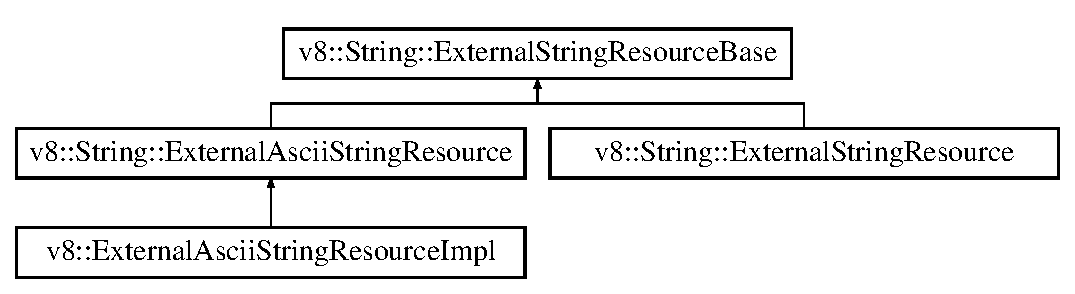
\includegraphics[height=3.000000cm]{classv8_1_1String_1_1ExternalStringResourceBase}
\end{center}
\end{figure}
\subsection*{Public Member Functions}
\begin{DoxyCompactItemize}
\item 
\mbox{\Hypertarget{classv8_1_1String_1_1ExternalStringResourceBase_aea69648f432efa7114684852d0ccfae6}\label{classv8_1_1String_1_1ExternalStringResourceBase_aea69648f432efa7114684852d0ccfae6}} 
virtual bool {\bfseries Is\+Compressible} () const
\end{DoxyCompactItemize}
\subsection*{Protected Member Functions}
\begin{DoxyCompactItemize}
\item 
virtual void \mbox{\hyperlink{classv8_1_1String_1_1ExternalStringResourceBase_af4720342ae31e1ab4656df3f15d069c0}{Dispose}} ()
\item 
\mbox{\Hypertarget{classv8_1_1String_1_1ExternalStringResourceBase_a2e9ebb706e3ebb401b1055a865b0ae0f}\label{classv8_1_1String_1_1ExternalStringResourceBase_a2e9ebb706e3ebb401b1055a865b0ae0f}} 
{\bfseries External\+String\+Resource\+Base} (const \mbox{\hyperlink{classv8_1_1String_1_1ExternalStringResourceBase}{External\+String\+Resource\+Base}} \&)=delete
\item 
\mbox{\Hypertarget{classv8_1_1String_1_1ExternalStringResourceBase_a17df23bb8aab9ee8c9658d6ebaf99e8c}\label{classv8_1_1String_1_1ExternalStringResourceBase_a17df23bb8aab9ee8c9658d6ebaf99e8c}} 
void {\bfseries operator=} (const \mbox{\hyperlink{classv8_1_1String_1_1ExternalStringResourceBase}{External\+String\+Resource\+Base}} \&)=delete
\end{DoxyCompactItemize}
\subsection*{Friends}
\begin{DoxyCompactItemize}
\item 
\mbox{\Hypertarget{classv8_1_1String_1_1ExternalStringResourceBase_a20a566310503e50c1b32668c772a14b2}\label{classv8_1_1String_1_1ExternalStringResourceBase_a20a566310503e50c1b32668c772a14b2}} 
class {\bfseries internal\+::\+Heap}
\item 
\mbox{\Hypertarget{classv8_1_1String_1_1ExternalStringResourceBase_a74072e7f09bdb13330b20ba10dcb8b55}\label{classv8_1_1String_1_1ExternalStringResourceBase_a74072e7f09bdb13330b20ba10dcb8b55}} 
class {\bfseries v8\+::\+String}
\end{DoxyCompactItemize}


\subsection{Member Function Documentation}
\mbox{\Hypertarget{classv8_1_1String_1_1ExternalStringResourceBase_af4720342ae31e1ab4656df3f15d069c0}\label{classv8_1_1String_1_1ExternalStringResourceBase_af4720342ae31e1ab4656df3f15d069c0}} 
\index{v8\+::\+String\+::\+External\+String\+Resource\+Base@{v8\+::\+String\+::\+External\+String\+Resource\+Base}!Dispose@{Dispose}}
\index{Dispose@{Dispose}!v8\+::\+String\+::\+External\+String\+Resource\+Base@{v8\+::\+String\+::\+External\+String\+Resource\+Base}}
\subsubsection{\texorpdfstring{Dispose()}{Dispose()}}
{\footnotesize\ttfamily virtual void v8\+::\+String\+::\+External\+String\+Resource\+Base\+::\+Dispose (\begin{DoxyParamCaption}{ }\end{DoxyParamCaption})\hspace{0.3cm}{\ttfamily [inline]}, {\ttfamily [protected]}, {\ttfamily [virtual]}}

Internally \mbox{\hyperlink{classv8_1_1V8}{V8}} will call this Dispose method when the external string resource is no longer needed. The default implementation will use the delete operator. This method can be overridden in subclasses to control how allocated external string resources are disposed. 

The documentation for this class was generated from the following file\+:\begin{DoxyCompactItemize}
\item 
v8/include/v8.\+h\end{DoxyCompactItemize}

\hypertarget{classv8_1_1Float32Array}{}\section{v8\+:\+:Float32\+Array Class Reference}
\label{classv8_1_1Float32Array}\index{v8\+::\+Float32\+Array@{v8\+::\+Float32\+Array}}


{\ttfamily \#include $<$v8.\+h$>$}

Inheritance diagram for v8\+:\+:Float32\+Array\+:\begin{figure}[H]
\begin{center}
\leavevmode
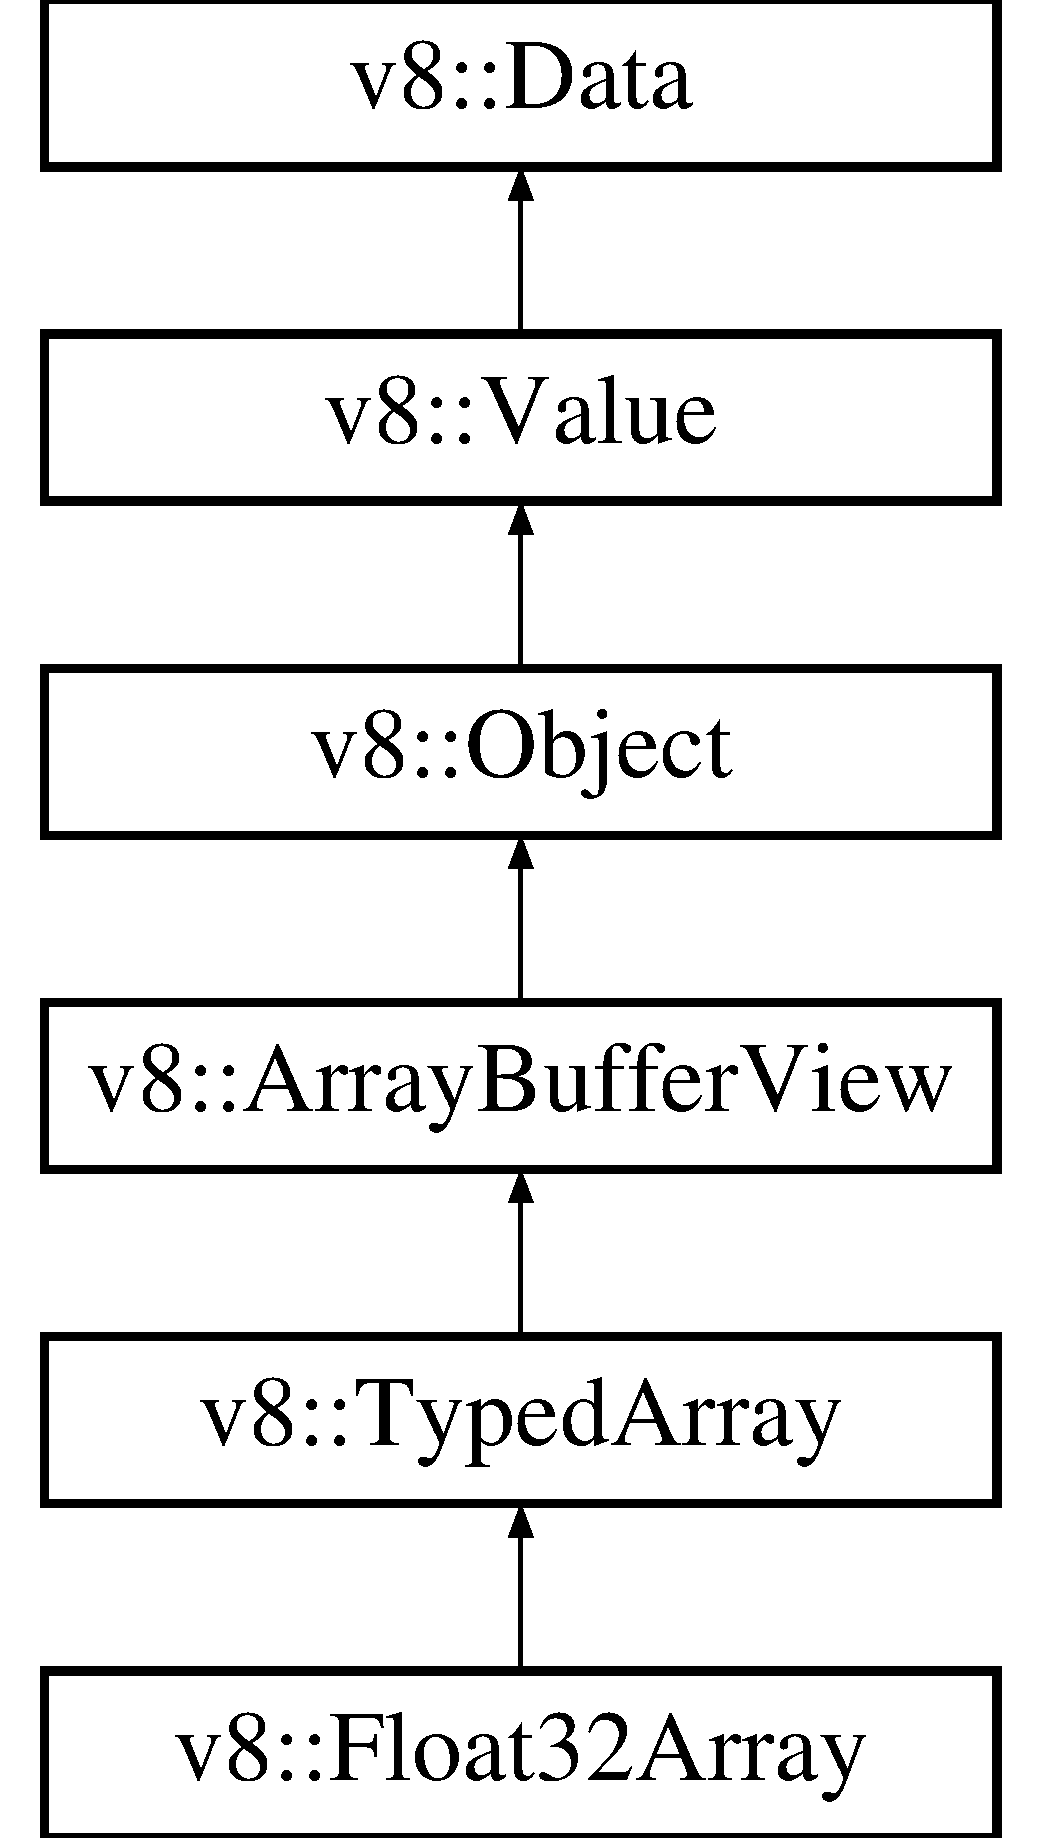
\includegraphics[height=6.000000cm]{classv8_1_1Float32Array}
\end{center}
\end{figure}
\subsection*{Static Public Member Functions}
\begin{DoxyCompactItemize}
\item 
\mbox{\Hypertarget{classv8_1_1Float32Array_af7e2ce97268849289d8ab38fd07fbf62}\label{classv8_1_1Float32Array_af7e2ce97268849289d8ab38fd07fbf62}} 
static \mbox{\hyperlink{classv8_1_1Local}{Local}}$<$ \mbox{\hyperlink{classv8_1_1Float32Array}{Float32\+Array}} $>$ {\bfseries New} (\mbox{\hyperlink{classv8_1_1Local}{Local}}$<$ \mbox{\hyperlink{classv8_1_1ArrayBuffer}{Array\+Buffer}} $>$ array\+\_\+buffer, size\+\_\+t byte\+\_\+offset, size\+\_\+t length)
\item 
\mbox{\Hypertarget{classv8_1_1Float32Array_af3140edf1f13845670f4e4ddd41200c3}\label{classv8_1_1Float32Array_af3140edf1f13845670f4e4ddd41200c3}} 
static \mbox{\hyperlink{classv8_1_1Local}{Local}}$<$ \mbox{\hyperlink{classv8_1_1Float32Array}{Float32\+Array}} $>$ {\bfseries New} (\mbox{\hyperlink{classv8_1_1Local}{Local}}$<$ \mbox{\hyperlink{classv8_1_1SharedArrayBuffer}{Shared\+Array\+Buffer}} $>$ shared\+\_\+array\+\_\+buffer, size\+\_\+t byte\+\_\+offset, size\+\_\+t length)
\item 
\mbox{\Hypertarget{classv8_1_1Float32Array_adf926d03cacd4b3901d7f9750671a350}\label{classv8_1_1Float32Array_adf926d03cacd4b3901d7f9750671a350}} 
static V8\+\_\+\+I\+N\+L\+I\+NE \mbox{\hyperlink{classv8_1_1Float32Array}{Float32\+Array}} $\ast$ {\bfseries Cast} (\mbox{\hyperlink{classv8_1_1Value}{Value}} $\ast$obj)
\end{DoxyCompactItemize}
\subsection*{Additional Inherited Members}


\subsection{Detailed Description}
An instance of \mbox{\hyperlink{classv8_1_1Float32Array}{Float32\+Array}} constructor (E\+S6 draft 15.\+13.\+6). 

The documentation for this class was generated from the following file\+:\begin{DoxyCompactItemize}
\item 
v8/include/v8.\+h\end{DoxyCompactItemize}

\hypertarget{classv8_1_1Float64Array}{}\section{v8\+:\+:Float64\+Array Class Reference}
\label{classv8_1_1Float64Array}\index{v8\+::\+Float64\+Array@{v8\+::\+Float64\+Array}}


{\ttfamily \#include $<$v8.\+h$>$}

Inheritance diagram for v8\+:\+:Float64\+Array\+:\begin{figure}[H]
\begin{center}
\leavevmode
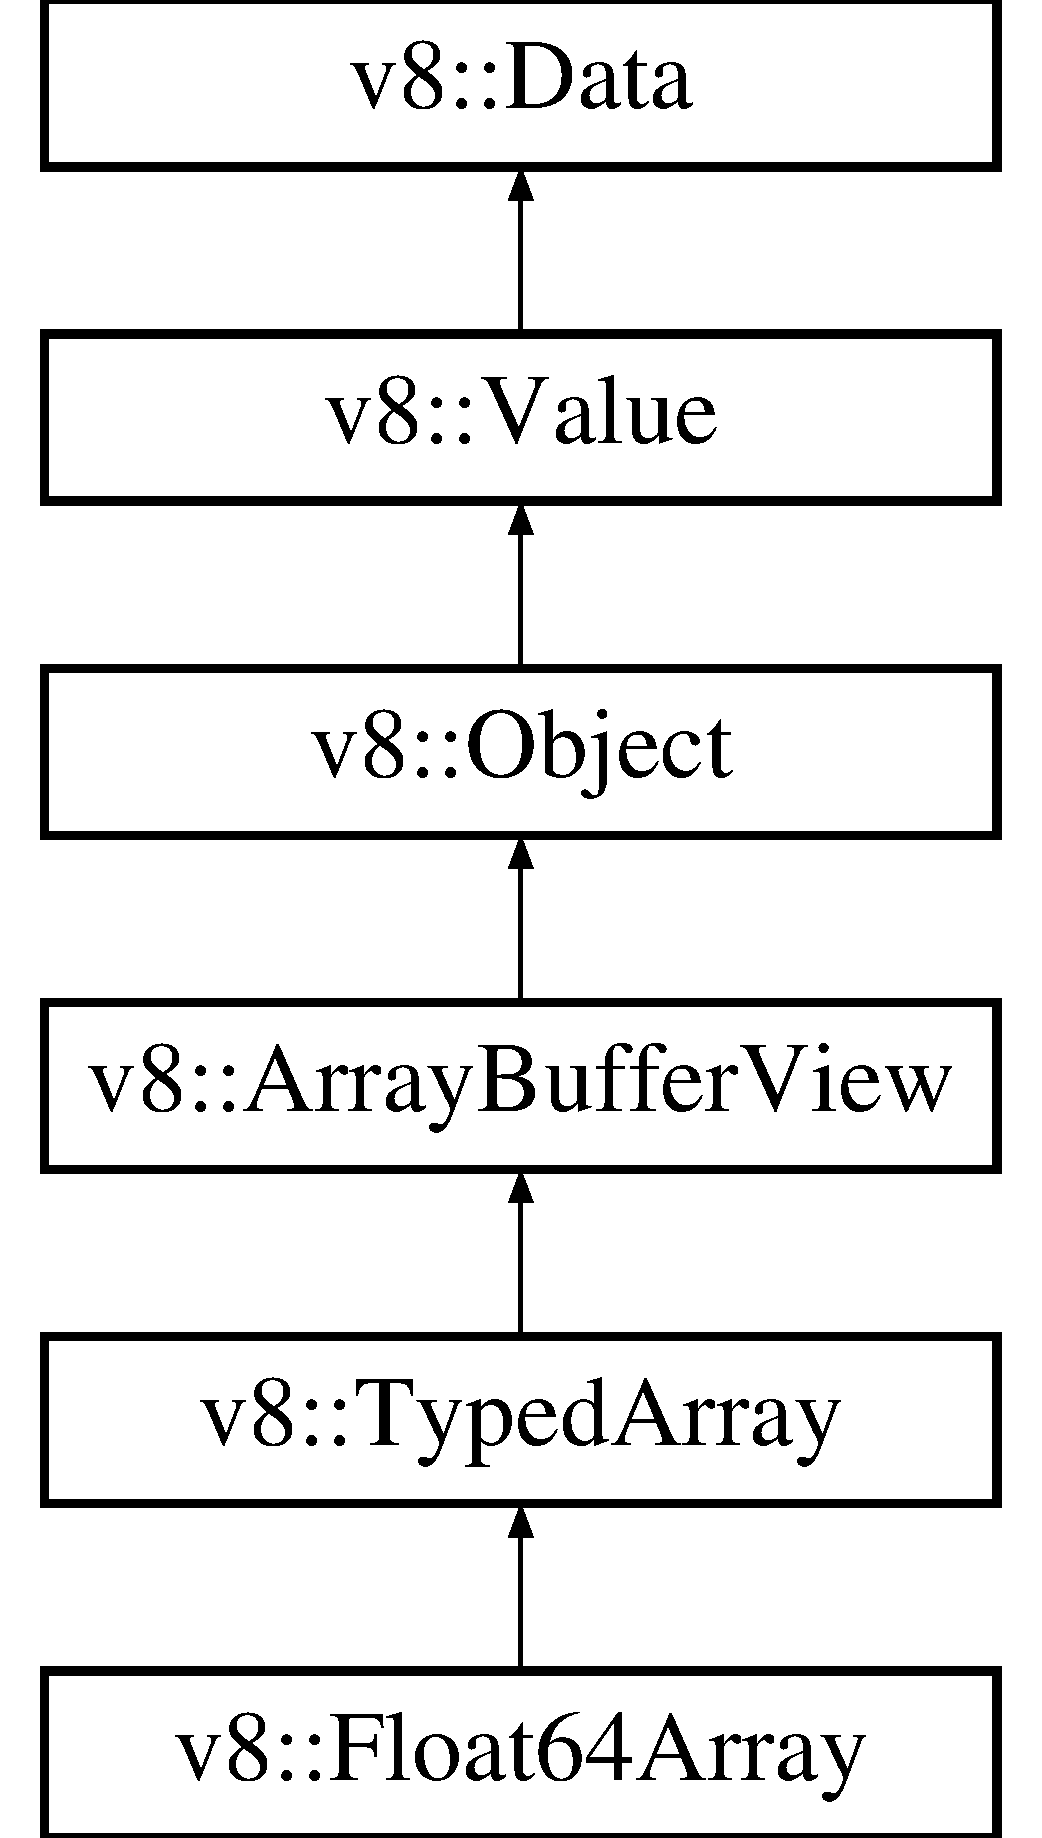
\includegraphics[height=6.000000cm]{classv8_1_1Float64Array}
\end{center}
\end{figure}
\subsection*{Static Public Member Functions}
\begin{DoxyCompactItemize}
\item 
\mbox{\Hypertarget{classv8_1_1Float64Array_a6e12e5ced578a357cfd049e036c4d6d6}\label{classv8_1_1Float64Array_a6e12e5ced578a357cfd049e036c4d6d6}} 
static \mbox{\hyperlink{classv8_1_1Local}{Local}}$<$ \mbox{\hyperlink{classv8_1_1Float64Array}{Float64\+Array}} $>$ {\bfseries New} (\mbox{\hyperlink{classv8_1_1Local}{Local}}$<$ \mbox{\hyperlink{classv8_1_1ArrayBuffer}{Array\+Buffer}} $>$ array\+\_\+buffer, size\+\_\+t byte\+\_\+offset, size\+\_\+t length)
\item 
\mbox{\Hypertarget{classv8_1_1Float64Array_aff414a8613e468f7deb29996f049e130}\label{classv8_1_1Float64Array_aff414a8613e468f7deb29996f049e130}} 
static \mbox{\hyperlink{classv8_1_1Local}{Local}}$<$ \mbox{\hyperlink{classv8_1_1Float64Array}{Float64\+Array}} $>$ {\bfseries New} (\mbox{\hyperlink{classv8_1_1Local}{Local}}$<$ \mbox{\hyperlink{classv8_1_1SharedArrayBuffer}{Shared\+Array\+Buffer}} $>$ shared\+\_\+array\+\_\+buffer, size\+\_\+t byte\+\_\+offset, size\+\_\+t length)
\item 
\mbox{\Hypertarget{classv8_1_1Float64Array_a936ee8e8cb2cb892cc5369e3ee6a7784}\label{classv8_1_1Float64Array_a936ee8e8cb2cb892cc5369e3ee6a7784}} 
static V8\+\_\+\+I\+N\+L\+I\+NE \mbox{\hyperlink{classv8_1_1Float64Array}{Float64\+Array}} $\ast$ {\bfseries Cast} (\mbox{\hyperlink{classv8_1_1Value}{Value}} $\ast$obj)
\end{DoxyCompactItemize}
\subsection*{Additional Inherited Members}


\subsection{Detailed Description}
An instance of \mbox{\hyperlink{classv8_1_1Float64Array}{Float64\+Array}} constructor (E\+S6 draft 15.\+13.\+6). 

The documentation for this class was generated from the following file\+:\begin{DoxyCompactItemize}
\item 
v8/include/v8.\+h\end{DoxyCompactItemize}

\hypertarget{classv8_1_1Function}{}\section{v8\+:\+:Function Class Reference}
\label{classv8_1_1Function}\index{v8\+::\+Function@{v8\+::\+Function}}


{\ttfamily \#include $<$v8.\+h$>$}

Inheritance diagram for v8\+:\+:Function\+:\begin{figure}[H]
\begin{center}
\leavevmode
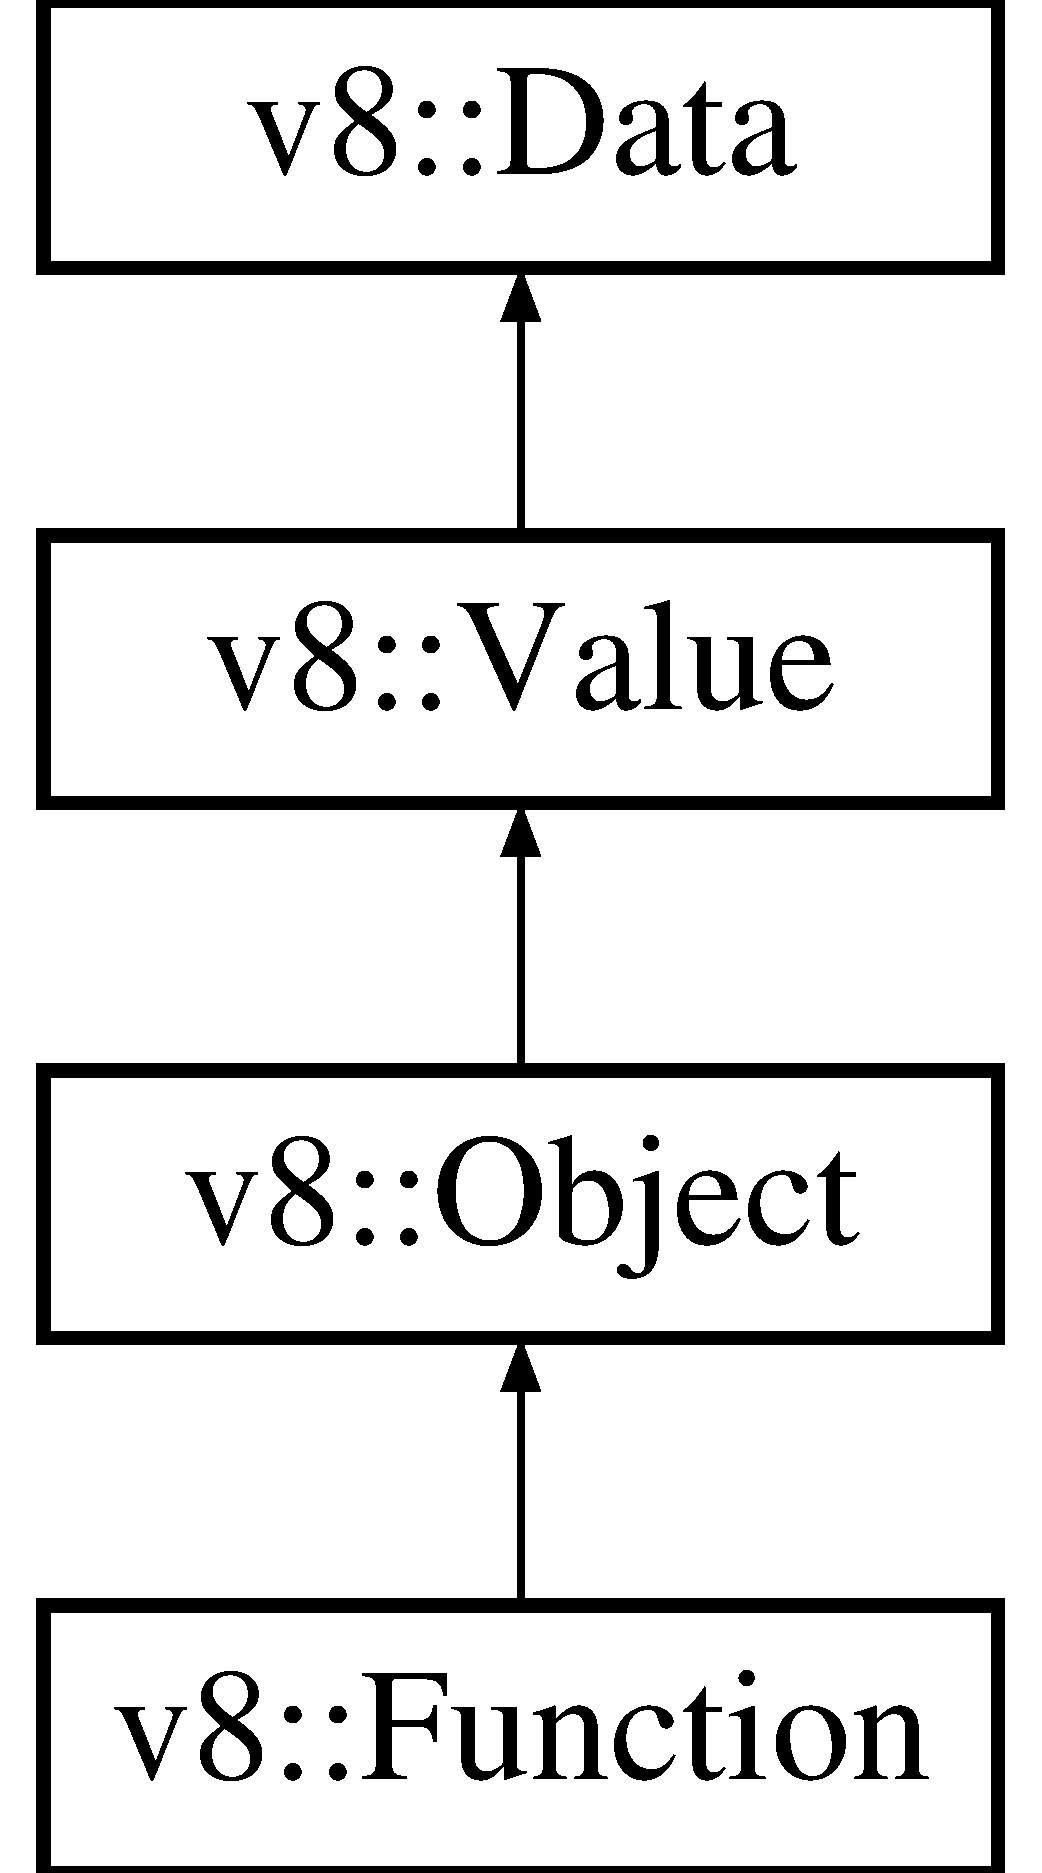
\includegraphics[height=4.000000cm]{classv8_1_1Function}
\end{center}
\end{figure}
\subsection*{Public Member Functions}
\begin{DoxyCompactItemize}
\item 
\mbox{\Hypertarget{classv8_1_1Function_ade57f07a67ad99630573b1c5b905a579}\label{classv8_1_1Function_ade57f07a67ad99630573b1c5b905a579}} 
V8\+\_\+\+W\+A\+R\+N\+\_\+\+U\+N\+U\+S\+E\+D\+\_\+\+R\+E\+S\+U\+LT \mbox{\hyperlink{classv8_1_1MaybeLocal}{Maybe\+Local}}$<$ \mbox{\hyperlink{classv8_1_1Object}{Object}} $>$ {\bfseries New\+Instance} (\mbox{\hyperlink{classv8_1_1Local}{Local}}$<$ Context $>$ context, int argc, \mbox{\hyperlink{classv8_1_1Local}{Local}}$<$ \mbox{\hyperlink{classv8_1_1Value}{Value}} $>$ argv\mbox{[}$\,$\mbox{]}) const
\item 
\mbox{\Hypertarget{classv8_1_1Function_ab491afc6bdf1d5174fe55d5cfad4ffe9}\label{classv8_1_1Function_ab491afc6bdf1d5174fe55d5cfad4ffe9}} 
V8\+\_\+\+W\+A\+R\+N\+\_\+\+U\+N\+U\+S\+E\+D\+\_\+\+R\+E\+S\+U\+LT \mbox{\hyperlink{classv8_1_1MaybeLocal}{Maybe\+Local}}$<$ \mbox{\hyperlink{classv8_1_1Object}{Object}} $>$ {\bfseries New\+Instance} (\mbox{\hyperlink{classv8_1_1Local}{Local}}$<$ Context $>$ context) const
\item 
V8\+\_\+\+W\+A\+R\+N\+\_\+\+U\+N\+U\+S\+E\+D\+\_\+\+R\+E\+S\+U\+LT \mbox{\hyperlink{classv8_1_1MaybeLocal}{Maybe\+Local}}$<$ \mbox{\hyperlink{classv8_1_1Object}{Object}} $>$ \mbox{\hyperlink{classv8_1_1Function_a3563e1a0f7de54f2d493a93a4e5e3b69}{New\+Instance\+With\+Side\+Effect\+Type}} (\mbox{\hyperlink{classv8_1_1Local}{Local}}$<$ Context $>$ context, int argc, \mbox{\hyperlink{classv8_1_1Local}{Local}}$<$ \mbox{\hyperlink{classv8_1_1Value}{Value}} $>$ argv\mbox{[}$\,$\mbox{]}, \mbox{\hyperlink{namespacev8_a29711319c2b9fc7716d65faee2f7b9cb}{Side\+Effect\+Type}} side\+\_\+effect\+\_\+type=Side\+Effect\+Type\+::k\+Has\+Side\+Effect) const
\item 
\mbox{\Hypertarget{classv8_1_1Function_a8d450b17b9bb911860ecf6c51ad468c0}\label{classv8_1_1Function_a8d450b17b9bb911860ecf6c51ad468c0}} 
{\bfseries V8\+\_\+\+D\+E\+P\+R\+E\+C\+A\+T\+ED} (\char`\"{}Use maybe version\char`\"{}, Local$<$ \mbox{\hyperlink{classv8_1_1Value}{Value}} $>$ Call(\mbox{\hyperlink{classv8_1_1Local}{Local}}$<$ \mbox{\hyperlink{classv8_1_1Value}{Value}} $>$ recv, int argc, \mbox{\hyperlink{classv8_1_1Local}{Local}}$<$ \mbox{\hyperlink{classv8_1_1Value}{Value}} $>$ argv\mbox{[}$\,$\mbox{]}))
\item 
\mbox{\Hypertarget{classv8_1_1Function_a70c400602e70488f7c066b950219a1ad}\label{classv8_1_1Function_a70c400602e70488f7c066b950219a1ad}} 
V8\+\_\+\+W\+A\+R\+N\+\_\+\+U\+N\+U\+S\+E\+D\+\_\+\+R\+E\+S\+U\+LT \mbox{\hyperlink{classv8_1_1MaybeLocal}{Maybe\+Local}}$<$ \mbox{\hyperlink{classv8_1_1Value}{Value}} $>$ {\bfseries Call} (\mbox{\hyperlink{classv8_1_1Local}{Local}}$<$ Context $>$ context, \mbox{\hyperlink{classv8_1_1Local}{Local}}$<$ \mbox{\hyperlink{classv8_1_1Value}{Value}} $>$ recv, int argc, \mbox{\hyperlink{classv8_1_1Local}{Local}}$<$ \mbox{\hyperlink{classv8_1_1Value}{Value}} $>$ argv\mbox{[}$\,$\mbox{]})
\item 
\mbox{\Hypertarget{classv8_1_1Function_aa9f51cea2036e0caa317e3955109856d}\label{classv8_1_1Function_aa9f51cea2036e0caa317e3955109856d}} 
void {\bfseries Set\+Name} (\mbox{\hyperlink{classv8_1_1Local}{Local}}$<$ \mbox{\hyperlink{classv8_1_1String}{String}} $>$ name)
\item 
\mbox{\Hypertarget{classv8_1_1Function_a2428c830a713b5e54f91cab42f281b01}\label{classv8_1_1Function_a2428c830a713b5e54f91cab42f281b01}} 
\mbox{\hyperlink{classv8_1_1Local}{Local}}$<$ \mbox{\hyperlink{classv8_1_1Value}{Value}} $>$ {\bfseries Get\+Name} () const
\item 
\mbox{\hyperlink{classv8_1_1Local}{Local}}$<$ \mbox{\hyperlink{classv8_1_1Value}{Value}} $>$ \mbox{\hyperlink{classv8_1_1Function_aa8cc6843d3df84ff5faf41af41cb07bc}{Get\+Inferred\+Name}} () const
\item 
\mbox{\hyperlink{classv8_1_1Local}{Local}}$<$ \mbox{\hyperlink{classv8_1_1Value}{Value}} $>$ \mbox{\hyperlink{classv8_1_1Function_a36946ff78ea0448d992957fa164187f1}{Get\+Debug\+Name}} () const
\item 
\mbox{\hyperlink{classv8_1_1Local}{Local}}$<$ \mbox{\hyperlink{classv8_1_1Value}{Value}} $>$ \mbox{\hyperlink{classv8_1_1Function_aa889eb7452de7c7a695c5981f603c7cb}{Get\+Display\+Name}} () const
\item 
int \mbox{\hyperlink{classv8_1_1Function_a616f966e538ec32182acd4acb7ee70bc}{Get\+Script\+Line\+Number}} () const
\item 
int \mbox{\hyperlink{classv8_1_1Function_a87bc63f97a9a39f83051570519fc63c2}{Get\+Script\+Column\+Number}} () const
\item 
int \mbox{\hyperlink{classv8_1_1Function_a5070c2657325ed6ca05ebb932c641438}{Script\+Id}} () const
\item 
\mbox{\hyperlink{classv8_1_1Local}{Local}}$<$ \mbox{\hyperlink{classv8_1_1Value}{Value}} $>$ \mbox{\hyperlink{classv8_1_1Function_a33bea08b5ff0c605bde07897cf1c431e}{Get\+Bound\+Function}} () const
\item 
\mbox{\Hypertarget{classv8_1_1Function_a79197c4c905cd1fb905f242c3d1d31cf}\label{classv8_1_1Function_a79197c4c905cd1fb905f242c3d1d31cf}} 
\mbox{\hyperlink{classv8_1_1ScriptOrigin}{Script\+Origin}} {\bfseries Get\+Script\+Origin} () const
\end{DoxyCompactItemize}
\subsection*{Static Public Member Functions}
\begin{DoxyCompactItemize}
\item 
static \mbox{\hyperlink{classv8_1_1MaybeLocal}{Maybe\+Local}}$<$ \mbox{\hyperlink{classv8_1_1Function}{Function}} $>$ \mbox{\hyperlink{classv8_1_1Function_afc51cb2669c3f8b6035c2a7f813d0040}{New}} (\mbox{\hyperlink{classv8_1_1Local}{Local}}$<$ Context $>$ context, Function\+Callback callback, \mbox{\hyperlink{classv8_1_1Local}{Local}}$<$ \mbox{\hyperlink{classv8_1_1Value}{Value}} $>$ data=\mbox{\hyperlink{classv8_1_1Local}{Local}}$<$ \mbox{\hyperlink{classv8_1_1Value}{Value}} $>$(), int length=0, Constructor\+Behavior behavior=Constructor\+Behavior\+::k\+Allow, \mbox{\hyperlink{namespacev8_a29711319c2b9fc7716d65faee2f7b9cb}{Side\+Effect\+Type}} side\+\_\+effect\+\_\+type=Side\+Effect\+Type\+::k\+Has\+Side\+Effect)
\item 
\mbox{\Hypertarget{classv8_1_1Function_a4ffb43746def98eb33536fa05bfecf16}\label{classv8_1_1Function_a4ffb43746def98eb33536fa05bfecf16}} 
static {\bfseries V8\+\_\+\+D\+E\+P\+R\+E\+C\+A\+T\+ED} (\char`\"{}Use maybe version\char`\"{}, Local$<$ \mbox{\hyperlink{classv8_1_1Function}{Function}} $>$ \mbox{\hyperlink{classv8_1_1Function_afc51cb2669c3f8b6035c2a7f813d0040}{New}}(Isolate $\ast$isolate, Function\+Callback callback, \mbox{\hyperlink{classv8_1_1Local}{Local}}$<$ \mbox{\hyperlink{classv8_1_1Value}{Value}} $>$ data=\mbox{\hyperlink{classv8_1_1Local}{Local}}$<$ \mbox{\hyperlink{classv8_1_1Value}{Value}} $>$(), int length=0))
\item 
\mbox{\Hypertarget{classv8_1_1Function_af24f38bcc0769519816cda1f6a154ff8}\label{classv8_1_1Function_af24f38bcc0769519816cda1f6a154ff8}} 
static V8\+\_\+\+I\+N\+L\+I\+NE \mbox{\hyperlink{classv8_1_1Function}{Function}} $\ast$ {\bfseries Cast} (\mbox{\hyperlink{classv8_1_1Value}{Value}} $\ast$obj)
\end{DoxyCompactItemize}
\subsection*{Static Public Attributes}
\begin{DoxyCompactItemize}
\item 
\mbox{\Hypertarget{classv8_1_1Function_acf0af24f79908e405a6ac435277596d9}\label{classv8_1_1Function_acf0af24f79908e405a6ac435277596d9}} 
static const int {\bfseries k\+Line\+Offset\+Not\+Found}
\end{DoxyCompactItemize}


\subsection{Detailed Description}
A Java\+Script function object (E\+C\+M\+A-\/262, 15.\+3). 

Definition at line 3995 of file v8.\+h.



\subsection{Member Function Documentation}
\mbox{\Hypertarget{classv8_1_1Function_a33bea08b5ff0c605bde07897cf1c431e}\label{classv8_1_1Function_a33bea08b5ff0c605bde07897cf1c431e}} 
\index{v8\+::\+Function@{v8\+::\+Function}!Get\+Bound\+Function@{Get\+Bound\+Function}}
\index{Get\+Bound\+Function@{Get\+Bound\+Function}!v8\+::\+Function@{v8\+::\+Function}}
\subsubsection{\texorpdfstring{Get\+Bound\+Function()}{GetBoundFunction()}}
{\footnotesize\ttfamily \mbox{\hyperlink{classv8_1_1Local}{Local}}$<$\mbox{\hyperlink{classv8_1_1Value}{Value}}$>$ v8\+::\+Function\+::\+Get\+Bound\+Function (\begin{DoxyParamCaption}{ }\end{DoxyParamCaption}) const}

Returns the original function if this function is bound, else returns v8\+::\+Undefined. \mbox{\Hypertarget{classv8_1_1Function_a36946ff78ea0448d992957fa164187f1}\label{classv8_1_1Function_a36946ff78ea0448d992957fa164187f1}} 
\index{v8\+::\+Function@{v8\+::\+Function}!Get\+Debug\+Name@{Get\+Debug\+Name}}
\index{Get\+Debug\+Name@{Get\+Debug\+Name}!v8\+::\+Function@{v8\+::\+Function}}
\subsubsection{\texorpdfstring{Get\+Debug\+Name()}{GetDebugName()}}
{\footnotesize\ttfamily \mbox{\hyperlink{classv8_1_1Local}{Local}}$<$\mbox{\hyperlink{classv8_1_1Value}{Value}}$>$ v8\+::\+Function\+::\+Get\+Debug\+Name (\begin{DoxyParamCaption}{ }\end{DoxyParamCaption}) const}

display\+Name if it is set, otherwise name if it is configured, otherwise function name, otherwise inferred name. \mbox{\Hypertarget{classv8_1_1Function_aa889eb7452de7c7a695c5981f603c7cb}\label{classv8_1_1Function_aa889eb7452de7c7a695c5981f603c7cb}} 
\index{v8\+::\+Function@{v8\+::\+Function}!Get\+Display\+Name@{Get\+Display\+Name}}
\index{Get\+Display\+Name@{Get\+Display\+Name}!v8\+::\+Function@{v8\+::\+Function}}
\subsubsection{\texorpdfstring{Get\+Display\+Name()}{GetDisplayName()}}
{\footnotesize\ttfamily \mbox{\hyperlink{classv8_1_1Local}{Local}}$<$\mbox{\hyperlink{classv8_1_1Value}{Value}}$>$ v8\+::\+Function\+::\+Get\+Display\+Name (\begin{DoxyParamCaption}{ }\end{DoxyParamCaption}) const}

User-\/defined name assigned to the \char`\"{}display\+Name\char`\"{} property of this function. Used to facilitate debugging and profiling of Java\+Script code. \mbox{\Hypertarget{classv8_1_1Function_aa8cc6843d3df84ff5faf41af41cb07bc}\label{classv8_1_1Function_aa8cc6843d3df84ff5faf41af41cb07bc}} 
\index{v8\+::\+Function@{v8\+::\+Function}!Get\+Inferred\+Name@{Get\+Inferred\+Name}}
\index{Get\+Inferred\+Name@{Get\+Inferred\+Name}!v8\+::\+Function@{v8\+::\+Function}}
\subsubsection{\texorpdfstring{Get\+Inferred\+Name()}{GetInferredName()}}
{\footnotesize\ttfamily \mbox{\hyperlink{classv8_1_1Local}{Local}}$<$\mbox{\hyperlink{classv8_1_1Value}{Value}}$>$ v8\+::\+Function\+::\+Get\+Inferred\+Name (\begin{DoxyParamCaption}{ }\end{DoxyParamCaption}) const}

\mbox{\hyperlink{classv8_1_1Name}{Name}} inferred from variable or property assignment of this function. Used to facilitate debugging and profiling of Java\+Script code written in an OO style, where many functions are anonymous but are assigned to object properties. \mbox{\Hypertarget{classv8_1_1Function_a87bc63f97a9a39f83051570519fc63c2}\label{classv8_1_1Function_a87bc63f97a9a39f83051570519fc63c2}} 
\index{v8\+::\+Function@{v8\+::\+Function}!Get\+Script\+Column\+Number@{Get\+Script\+Column\+Number}}
\index{Get\+Script\+Column\+Number@{Get\+Script\+Column\+Number}!v8\+::\+Function@{v8\+::\+Function}}
\subsubsection{\texorpdfstring{Get\+Script\+Column\+Number()}{GetScriptColumnNumber()}}
{\footnotesize\ttfamily int v8\+::\+Function\+::\+Get\+Script\+Column\+Number (\begin{DoxyParamCaption}{ }\end{DoxyParamCaption}) const}

Returns zero based column number of function body and k\+Line\+Offset\+Not\+Found if no information available. \mbox{\Hypertarget{classv8_1_1Function_a616f966e538ec32182acd4acb7ee70bc}\label{classv8_1_1Function_a616f966e538ec32182acd4acb7ee70bc}} 
\index{v8\+::\+Function@{v8\+::\+Function}!Get\+Script\+Line\+Number@{Get\+Script\+Line\+Number}}
\index{Get\+Script\+Line\+Number@{Get\+Script\+Line\+Number}!v8\+::\+Function@{v8\+::\+Function}}
\subsubsection{\texorpdfstring{Get\+Script\+Line\+Number()}{GetScriptLineNumber()}}
{\footnotesize\ttfamily int v8\+::\+Function\+::\+Get\+Script\+Line\+Number (\begin{DoxyParamCaption}{ }\end{DoxyParamCaption}) const}

Returns zero based line number of function body and k\+Line\+Offset\+Not\+Found if no information available. \mbox{\Hypertarget{classv8_1_1Function_afc51cb2669c3f8b6035c2a7f813d0040}\label{classv8_1_1Function_afc51cb2669c3f8b6035c2a7f813d0040}} 
\index{v8\+::\+Function@{v8\+::\+Function}!New@{New}}
\index{New@{New}!v8\+::\+Function@{v8\+::\+Function}}
\subsubsection{\texorpdfstring{New()}{New()}}
{\footnotesize\ttfamily static \mbox{\hyperlink{classv8_1_1MaybeLocal}{Maybe\+Local}}$<$\mbox{\hyperlink{classv8_1_1Function}{Function}}$>$ v8\+::\+Function\+::\+New (\begin{DoxyParamCaption}\item[{\mbox{\hyperlink{classv8_1_1Local}{Local}}$<$ Context $>$}]{context,  }\item[{Function\+Callback}]{callback,  }\item[{\mbox{\hyperlink{classv8_1_1Local}{Local}}$<$ \mbox{\hyperlink{classv8_1_1Value}{Value}} $>$}]{data = {\ttfamily \mbox{\hyperlink{classv8_1_1Local}{Local}}$<$~\mbox{\hyperlink{classv8_1_1Value}{Value}}~$>$()},  }\item[{int}]{length = {\ttfamily 0},  }\item[{Constructor\+Behavior}]{behavior = {\ttfamily ConstructorBehavior\+:\+:kAllow},  }\item[{\mbox{\hyperlink{namespacev8_a29711319c2b9fc7716d65faee2f7b9cb}{Side\+Effect\+Type}}}]{side\+\_\+effect\+\_\+type = {\ttfamily SideEffectType\+:\+:kHasSideEffect} }\end{DoxyParamCaption})\hspace{0.3cm}{\ttfamily [static]}}

Create a function in the current execution context for a given Function\+Callback. \mbox{\Hypertarget{classv8_1_1Function_a3563e1a0f7de54f2d493a93a4e5e3b69}\label{classv8_1_1Function_a3563e1a0f7de54f2d493a93a4e5e3b69}} 
\index{v8\+::\+Function@{v8\+::\+Function}!New\+Instance\+With\+Side\+Effect\+Type@{New\+Instance\+With\+Side\+Effect\+Type}}
\index{New\+Instance\+With\+Side\+Effect\+Type@{New\+Instance\+With\+Side\+Effect\+Type}!v8\+::\+Function@{v8\+::\+Function}}
\subsubsection{\texorpdfstring{New\+Instance\+With\+Side\+Effect\+Type()}{NewInstanceWithSideEffectType()}}
{\footnotesize\ttfamily V8\+\_\+\+W\+A\+R\+N\+\_\+\+U\+N\+U\+S\+E\+D\+\_\+\+R\+E\+S\+U\+LT \mbox{\hyperlink{classv8_1_1MaybeLocal}{Maybe\+Local}}$<$\mbox{\hyperlink{classv8_1_1Object}{Object}}$>$ v8\+::\+Function\+::\+New\+Instance\+With\+Side\+Effect\+Type (\begin{DoxyParamCaption}\item[{\mbox{\hyperlink{classv8_1_1Local}{Local}}$<$ Context $>$}]{context,  }\item[{int}]{argc,  }\item[{\mbox{\hyperlink{classv8_1_1Local}{Local}}$<$ \mbox{\hyperlink{classv8_1_1Value}{Value}} $>$}]{argv\mbox{[}$\,$\mbox{]},  }\item[{\mbox{\hyperlink{namespacev8_a29711319c2b9fc7716d65faee2f7b9cb}{Side\+Effect\+Type}}}]{side\+\_\+effect\+\_\+type = {\ttfamily SideEffectType\+:\+:kHasSideEffect} }\end{DoxyParamCaption}) const}

When side effect checks are enabled, passing k\+Has\+No\+Side\+Effect allows the constructor to be invoked without throwing. Calls made within the constructor are still checked. \mbox{\Hypertarget{classv8_1_1Function_a5070c2657325ed6ca05ebb932c641438}\label{classv8_1_1Function_a5070c2657325ed6ca05ebb932c641438}} 
\index{v8\+::\+Function@{v8\+::\+Function}!Script\+Id@{Script\+Id}}
\index{Script\+Id@{Script\+Id}!v8\+::\+Function@{v8\+::\+Function}}
\subsubsection{\texorpdfstring{Script\+Id()}{ScriptId()}}
{\footnotesize\ttfamily int v8\+::\+Function\+::\+Script\+Id (\begin{DoxyParamCaption}{ }\end{DoxyParamCaption}) const}

Returns script\+Id. 

The documentation for this class was generated from the following file\+:\begin{DoxyCompactItemize}
\item 
v8/include/v8.\+h\end{DoxyCompactItemize}

\hypertarget{classv8_1_1FunctionCallbackInfo}{}\section{v8\+:\+:Function\+Callback\+Info$<$ T $>$ Class Template Reference}
\label{classv8_1_1FunctionCallbackInfo}\index{v8\+::\+Function\+Callback\+Info$<$ T $>$@{v8\+::\+Function\+Callback\+Info$<$ T $>$}}


{\ttfamily \#include $<$v8.\+h$>$}

\subsection*{Public Member Functions}
\begin{DoxyCompactItemize}
\item 
V8\+\_\+\+I\+N\+L\+I\+NE int \mbox{\hyperlink{classv8_1_1FunctionCallbackInfo_af97dd3f1cb01ed039f9479152ad63a84}{Length}} () const
\item 
V8\+\_\+\+I\+N\+L\+I\+NE \mbox{\hyperlink{classv8_1_1Local}{Local}}$<$ \mbox{\hyperlink{classv8_1_1Value}{Value}} $>$ \mbox{\hyperlink{classv8_1_1FunctionCallbackInfo_a77dce5cad7b198c4181a522e9e0ab10f}{operator\mbox{[}$\,$\mbox{]}}} (int i) const
\item 
V8\+\_\+\+I\+N\+L\+I\+NE \mbox{\hyperlink{classv8_1_1Local}{Local}}$<$ \mbox{\hyperlink{classv8_1_1Object}{Object}} $>$ \mbox{\hyperlink{classv8_1_1FunctionCallbackInfo_a4ddfd6d21732dff1c4c55d5441a8a5ca}{This}} () const
\item 
V8\+\_\+\+I\+N\+L\+I\+NE \mbox{\hyperlink{classv8_1_1Local}{Local}}$<$ \mbox{\hyperlink{classv8_1_1Object}{Object}} $>$ \mbox{\hyperlink{classv8_1_1FunctionCallbackInfo_a708ab465862ed796e3b0b3c37ba05044}{Holder}} () const
\item 
V8\+\_\+\+I\+N\+L\+I\+NE \mbox{\hyperlink{classv8_1_1Local}{Local}}$<$ \mbox{\hyperlink{classv8_1_1Value}{Value}} $>$ \mbox{\hyperlink{classv8_1_1FunctionCallbackInfo_aa04f4c5c984db26a90b591f34550e6fa}{New\+Target}} () const
\item 
V8\+\_\+\+I\+N\+L\+I\+NE bool \mbox{\hyperlink{classv8_1_1FunctionCallbackInfo_ad2105b93e9b4d02f42b7338fa5950cbc}{Is\+Construct\+Call}} () const
\item 
V8\+\_\+\+I\+N\+L\+I\+NE \mbox{\hyperlink{classv8_1_1Local}{Local}}$<$ \mbox{\hyperlink{classv8_1_1Value}{Value}} $>$ \mbox{\hyperlink{classv8_1_1FunctionCallbackInfo_ab0ebfc2ea43af2fdfc3d085272bf499f}{Data}} () const
\item 
V8\+\_\+\+I\+N\+L\+I\+NE Isolate $\ast$ \mbox{\hyperlink{classv8_1_1FunctionCallbackInfo_a7eee713a6f95d5707ce788861754682f}{Get\+Isolate}} () const
\item 
V8\+\_\+\+I\+N\+L\+I\+NE \mbox{\hyperlink{classv8_1_1ReturnValue}{Return\+Value}}$<$ T $>$ \mbox{\hyperlink{classv8_1_1FunctionCallbackInfo_a2cb41afe1e098a46d27d901b4cc1e6f5}{Get\+Return\+Value}} () const
\end{DoxyCompactItemize}
\subsection*{Static Public Attributes}
\begin{DoxyCompactItemize}
\item 
\mbox{\Hypertarget{classv8_1_1FunctionCallbackInfo_a1e5248c2d40840270829882feaaa9d34}\label{classv8_1_1FunctionCallbackInfo_a1e5248c2d40840270829882feaaa9d34}} 
static const int {\bfseries k\+Args\+Length} = 6
\end{DoxyCompactItemize}
\subsection*{Protected Member Functions}
\begin{DoxyCompactItemize}
\item 
\mbox{\Hypertarget{classv8_1_1FunctionCallbackInfo_a34ca4a2f13fa2479a340d5cfd8efaca1}\label{classv8_1_1FunctionCallbackInfo_a34ca4a2f13fa2479a340d5cfd8efaca1}} 
V8\+\_\+\+I\+N\+L\+I\+NE {\bfseries Function\+Callback\+Info} (internal\+::\+Address $\ast$implicit\+\_\+args, internal\+::\+Address $\ast$values, int length)
\end{DoxyCompactItemize}
\subsection*{Protected Attributes}
\begin{DoxyCompactItemize}
\item 
\mbox{\Hypertarget{classv8_1_1FunctionCallbackInfo_a589fda1e686768fb49af5f5ea9e6549e}\label{classv8_1_1FunctionCallbackInfo_a589fda1e686768fb49af5f5ea9e6549e}} 
internal\+::\+Address $\ast$ {\bfseries implicit\+\_\+args\+\_\+}
\item 
\mbox{\Hypertarget{classv8_1_1FunctionCallbackInfo_a1692383567930ec69c51ddfd9207744e}\label{classv8_1_1FunctionCallbackInfo_a1692383567930ec69c51ddfd9207744e}} 
internal\+::\+Address $\ast$ {\bfseries values\+\_\+}
\item 
\mbox{\Hypertarget{classv8_1_1FunctionCallbackInfo_ab250ace06b495beb6f14b192eff77005}\label{classv8_1_1FunctionCallbackInfo_ab250ace06b495beb6f14b192eff77005}} 
int {\bfseries length\+\_\+}
\end{DoxyCompactItemize}
\subsection*{Static Protected Attributes}
\begin{DoxyCompactItemize}
\item 
\mbox{\Hypertarget{classv8_1_1FunctionCallbackInfo_a073824921daf8600fb9c00c50ee8ef0c}\label{classv8_1_1FunctionCallbackInfo_a073824921daf8600fb9c00c50ee8ef0c}} 
static const int {\bfseries k\+Holder\+Index} = 0
\item 
\mbox{\Hypertarget{classv8_1_1FunctionCallbackInfo_a0e2fbe5a323276263c848ea8050a34eb}\label{classv8_1_1FunctionCallbackInfo_a0e2fbe5a323276263c848ea8050a34eb}} 
static const int {\bfseries k\+Isolate\+Index} = 1
\item 
\mbox{\Hypertarget{classv8_1_1FunctionCallbackInfo_a0b32b5613fe2f0cd139d9dffc0916d09}\label{classv8_1_1FunctionCallbackInfo_a0b32b5613fe2f0cd139d9dffc0916d09}} 
static const int {\bfseries k\+Return\+Value\+Default\+Value\+Index} = 2
\item 
\mbox{\Hypertarget{classv8_1_1FunctionCallbackInfo_abb339e201184ebe2502a1202d54201ca}\label{classv8_1_1FunctionCallbackInfo_abb339e201184ebe2502a1202d54201ca}} 
static const int {\bfseries k\+Return\+Value\+Index} = 3
\item 
\mbox{\Hypertarget{classv8_1_1FunctionCallbackInfo_a152c34c5b2f8c55d04d6d541bf8a4544}\label{classv8_1_1FunctionCallbackInfo_a152c34c5b2f8c55d04d6d541bf8a4544}} 
static const int {\bfseries k\+Data\+Index} = 4
\item 
\mbox{\Hypertarget{classv8_1_1FunctionCallbackInfo_a23e70f4737b7e205dc91b972d75fbd9c}\label{classv8_1_1FunctionCallbackInfo_a23e70f4737b7e205dc91b972d75fbd9c}} 
static const int {\bfseries k\+New\+Target\+Index} = 5
\end{DoxyCompactItemize}
\subsection*{Friends}
\begin{DoxyCompactItemize}
\item 
\mbox{\Hypertarget{classv8_1_1FunctionCallbackInfo_aac7268b20857fd75b69b86ded46d0f34}\label{classv8_1_1FunctionCallbackInfo_aac7268b20857fd75b69b86ded46d0f34}} 
class {\bfseries internal\+::\+Function\+Callback\+Arguments}
\item 
\mbox{\Hypertarget{classv8_1_1FunctionCallbackInfo_a02d869d89b14ddd1717429c2106f955a}\label{classv8_1_1FunctionCallbackInfo_a02d869d89b14ddd1717429c2106f955a}} 
class {\bfseries internal\+::\+Custom\+Arguments$<$ Function\+Callback\+Info $>$}
\item 
\mbox{\Hypertarget{classv8_1_1FunctionCallbackInfo_aa7dc5c9ac169be8c0feb25eae56c35fe}\label{classv8_1_1FunctionCallbackInfo_aa7dc5c9ac169be8c0feb25eae56c35fe}} 
class {\bfseries debug\+::\+Console\+Call\+Arguments}
\end{DoxyCompactItemize}


\subsection{Detailed Description}
\subsubsection*{template$<$typename T$>$\newline
class v8\+::\+Function\+Callback\+Info$<$ T $>$}

The argument information given to function call callbacks. This class provides access to information about the context of the call, including the receiver, the number and values of arguments, and the holder of the function. 

Definition at line 104 of file v8.\+h.



\subsection{Member Function Documentation}
\mbox{\Hypertarget{classv8_1_1FunctionCallbackInfo_ab0ebfc2ea43af2fdfc3d085272bf499f}\label{classv8_1_1FunctionCallbackInfo_ab0ebfc2ea43af2fdfc3d085272bf499f}} 
\index{v8\+::\+Function\+Callback\+Info@{v8\+::\+Function\+Callback\+Info}!Data@{Data}}
\index{Data@{Data}!v8\+::\+Function\+Callback\+Info@{v8\+::\+Function\+Callback\+Info}}
\subsubsection{\texorpdfstring{Data()}{Data()}}
{\footnotesize\ttfamily template$<$typename T $>$ \\
\mbox{\hyperlink{classv8_1_1Local}{Local}}$<$ \mbox{\hyperlink{classv8_1_1Value}{Value}} $>$ \mbox{\hyperlink{classv8_1_1FunctionCallbackInfo}{v8\+::\+Function\+Callback\+Info}}$<$ T $>$\+::\mbox{\hyperlink{classv8_1_1Data}{Data}} (\begin{DoxyParamCaption}{ }\end{DoxyParamCaption}) const}

The data argument specified when creating the callback. 

Definition at line 9727 of file v8.\+h.

\mbox{\Hypertarget{classv8_1_1FunctionCallbackInfo_a7eee713a6f95d5707ce788861754682f}\label{classv8_1_1FunctionCallbackInfo_a7eee713a6f95d5707ce788861754682f}} 
\index{v8\+::\+Function\+Callback\+Info@{v8\+::\+Function\+Callback\+Info}!Get\+Isolate@{Get\+Isolate}}
\index{Get\+Isolate@{Get\+Isolate}!v8\+::\+Function\+Callback\+Info@{v8\+::\+Function\+Callback\+Info}}
\subsubsection{\texorpdfstring{Get\+Isolate()}{GetIsolate()}}
{\footnotesize\ttfamily template$<$typename T $>$ \\
Isolate $\ast$ \mbox{\hyperlink{classv8_1_1FunctionCallbackInfo}{v8\+::\+Function\+Callback\+Info}}$<$ T $>$\+::Get\+Isolate (\begin{DoxyParamCaption}{ }\end{DoxyParamCaption}) const}

The current Isolate. 

Definition at line 9733 of file v8.\+h.

\mbox{\Hypertarget{classv8_1_1FunctionCallbackInfo_a2cb41afe1e098a46d27d901b4cc1e6f5}\label{classv8_1_1FunctionCallbackInfo_a2cb41afe1e098a46d27d901b4cc1e6f5}} 
\index{v8\+::\+Function\+Callback\+Info@{v8\+::\+Function\+Callback\+Info}!Get\+Return\+Value@{Get\+Return\+Value}}
\index{Get\+Return\+Value@{Get\+Return\+Value}!v8\+::\+Function\+Callback\+Info@{v8\+::\+Function\+Callback\+Info}}
\subsubsection{\texorpdfstring{Get\+Return\+Value()}{GetReturnValue()}}
{\footnotesize\ttfamily template$<$typename T $>$ \\
\mbox{\hyperlink{classv8_1_1ReturnValue}{Return\+Value}}$<$ T $>$ \mbox{\hyperlink{classv8_1_1FunctionCallbackInfo}{v8\+::\+Function\+Callback\+Info}}$<$ T $>$\+::Get\+Return\+Value (\begin{DoxyParamCaption}{ }\end{DoxyParamCaption}) const}

The \mbox{\hyperlink{classv8_1_1ReturnValue}{Return\+Value}} for the call. 

Definition at line 9739 of file v8.\+h.

\mbox{\Hypertarget{classv8_1_1FunctionCallbackInfo_a708ab465862ed796e3b0b3c37ba05044}\label{classv8_1_1FunctionCallbackInfo_a708ab465862ed796e3b0b3c37ba05044}} 
\index{v8\+::\+Function\+Callback\+Info@{v8\+::\+Function\+Callback\+Info}!Holder@{Holder}}
\index{Holder@{Holder}!v8\+::\+Function\+Callback\+Info@{v8\+::\+Function\+Callback\+Info}}
\subsubsection{\texorpdfstring{Holder()}{Holder()}}
{\footnotesize\ttfamily template$<$typename T $>$ \\
\mbox{\hyperlink{classv8_1_1Local}{Local}}$<$ \mbox{\hyperlink{classv8_1_1Object}{Object}} $>$ \mbox{\hyperlink{classv8_1_1FunctionCallbackInfo}{v8\+::\+Function\+Callback\+Info}}$<$ T $>$\+::Holder (\begin{DoxyParamCaption}{ }\end{DoxyParamCaption}) const}

If the callback was created without a \mbox{\hyperlink{classv8_1_1Signature}{Signature}}, this is the same value as \mbox{\hyperlink{classv8_1_1FunctionCallbackInfo_a4ddfd6d21732dff1c4c55d5441a8a5ca}{This()}}. If there is a signature, and the signature didn\textquotesingle{}t match \mbox{\hyperlink{classv8_1_1FunctionCallbackInfo_a4ddfd6d21732dff1c4c55d5441a8a5ca}{This()}} but one of its hidden prototypes, this will be the respective hidden prototype.

Note that this is not the prototype of \mbox{\hyperlink{classv8_1_1FunctionCallbackInfo_a4ddfd6d21732dff1c4c55d5441a8a5ca}{This()}} on which the accessor referencing this callback was found (which in V8 internally is often referred to as holder \mbox{[}sic\mbox{]}). 

Definition at line 9715 of file v8.\+h.

\mbox{\Hypertarget{classv8_1_1FunctionCallbackInfo_ad2105b93e9b4d02f42b7338fa5950cbc}\label{classv8_1_1FunctionCallbackInfo_ad2105b93e9b4d02f42b7338fa5950cbc}} 
\index{v8\+::\+Function\+Callback\+Info@{v8\+::\+Function\+Callback\+Info}!Is\+Construct\+Call@{Is\+Construct\+Call}}
\index{Is\+Construct\+Call@{Is\+Construct\+Call}!v8\+::\+Function\+Callback\+Info@{v8\+::\+Function\+Callback\+Info}}
\subsubsection{\texorpdfstring{Is\+Construct\+Call()}{IsConstructCall()}}
{\footnotesize\ttfamily template$<$typename T $>$ \\
bool \mbox{\hyperlink{classv8_1_1FunctionCallbackInfo}{v8\+::\+Function\+Callback\+Info}}$<$ T $>$\+::Is\+Construct\+Call (\begin{DoxyParamCaption}{ }\end{DoxyParamCaption}) const}

Indicates whether this is a regular call or a construct call. 

Definition at line 9745 of file v8.\+h.

\mbox{\Hypertarget{classv8_1_1FunctionCallbackInfo_af97dd3f1cb01ed039f9479152ad63a84}\label{classv8_1_1FunctionCallbackInfo_af97dd3f1cb01ed039f9479152ad63a84}} 
\index{v8\+::\+Function\+Callback\+Info@{v8\+::\+Function\+Callback\+Info}!Length@{Length}}
\index{Length@{Length}!v8\+::\+Function\+Callback\+Info@{v8\+::\+Function\+Callback\+Info}}
\subsubsection{\texorpdfstring{Length()}{Length()}}
{\footnotesize\ttfamily template$<$typename T $>$ \\
int \mbox{\hyperlink{classv8_1_1FunctionCallbackInfo}{v8\+::\+Function\+Callback\+Info}}$<$ T $>$\+::Length (\begin{DoxyParamCaption}{ }\end{DoxyParamCaption}) const}

The number of available arguments. 

Definition at line 9751 of file v8.\+h.

\mbox{\Hypertarget{classv8_1_1FunctionCallbackInfo_aa04f4c5c984db26a90b591f34550e6fa}\label{classv8_1_1FunctionCallbackInfo_aa04f4c5c984db26a90b591f34550e6fa}} 
\index{v8\+::\+Function\+Callback\+Info@{v8\+::\+Function\+Callback\+Info}!New\+Target@{New\+Target}}
\index{New\+Target@{New\+Target}!v8\+::\+Function\+Callback\+Info@{v8\+::\+Function\+Callback\+Info}}
\subsubsection{\texorpdfstring{New\+Target()}{NewTarget()}}
{\footnotesize\ttfamily template$<$typename T $>$ \\
\mbox{\hyperlink{classv8_1_1Local}{Local}}$<$ \mbox{\hyperlink{classv8_1_1Value}{Value}} $>$ \mbox{\hyperlink{classv8_1_1FunctionCallbackInfo}{v8\+::\+Function\+Callback\+Info}}$<$ T $>$\+::New\+Target (\begin{DoxyParamCaption}{ }\end{DoxyParamCaption}) const}

For construct calls, this returns the \char`\"{}new.\+target\char`\"{} value. 

Definition at line 9721 of file v8.\+h.

\mbox{\Hypertarget{classv8_1_1FunctionCallbackInfo_a77dce5cad7b198c4181a522e9e0ab10f}\label{classv8_1_1FunctionCallbackInfo_a77dce5cad7b198c4181a522e9e0ab10f}} 
\index{v8\+::\+Function\+Callback\+Info@{v8\+::\+Function\+Callback\+Info}!operator\mbox{[}\mbox{]}@{operator[]}}
\index{operator\mbox{[}\mbox{]}@{operator[]}!v8\+::\+Function\+Callback\+Info@{v8\+::\+Function\+Callback\+Info}}
\subsubsection{\texorpdfstring{operator[]()}{operator[]()}}
{\footnotesize\ttfamily template$<$typename T $>$ \\
\mbox{\hyperlink{classv8_1_1Local}{Local}}$<$ \mbox{\hyperlink{classv8_1_1Value}{Value}} $>$ \mbox{\hyperlink{classv8_1_1FunctionCallbackInfo}{v8\+::\+Function\+Callback\+Info}}$<$ T $>$\+::operator\mbox{[}$\,$\mbox{]} (\begin{DoxyParamCaption}\item[{int}]{i }\end{DoxyParamCaption}) const}

Accessor for the available arguments. 

Definition at line 9702 of file v8.\+h.

\mbox{\Hypertarget{classv8_1_1FunctionCallbackInfo_a4ddfd6d21732dff1c4c55d5441a8a5ca}\label{classv8_1_1FunctionCallbackInfo_a4ddfd6d21732dff1c4c55d5441a8a5ca}} 
\index{v8\+::\+Function\+Callback\+Info@{v8\+::\+Function\+Callback\+Info}!This@{This}}
\index{This@{This}!v8\+::\+Function\+Callback\+Info@{v8\+::\+Function\+Callback\+Info}}
\subsubsection{\texorpdfstring{This()}{This()}}
{\footnotesize\ttfamily template$<$typename T $>$ \\
\mbox{\hyperlink{classv8_1_1Local}{Local}}$<$ \mbox{\hyperlink{classv8_1_1Object}{Object}} $>$ \mbox{\hyperlink{classv8_1_1FunctionCallbackInfo}{v8\+::\+Function\+Callback\+Info}}$<$ T $>$\+::This (\begin{DoxyParamCaption}{ }\end{DoxyParamCaption}) const}

Returns the receiver. This corresponds to the \char`\"{}this\char`\"{} value. 

Definition at line 9709 of file v8.\+h.



The documentation for this class was generated from the following file\+:\begin{DoxyCompactItemize}
\item 
v8/include/v8.\+h\end{DoxyCompactItemize}

\hypertarget{classv8_1_1FunctionTemplate}{}\section{v8\+:\+:Function\+Template Class Reference}
\label{classv8_1_1FunctionTemplate}\index{v8\+::\+Function\+Template@{v8\+::\+Function\+Template}}


{\ttfamily \#include $<$v8.\+h$>$}

Inheritance diagram for v8\+:\+:Function\+Template\+:\begin{figure}[H]
\begin{center}
\leavevmode
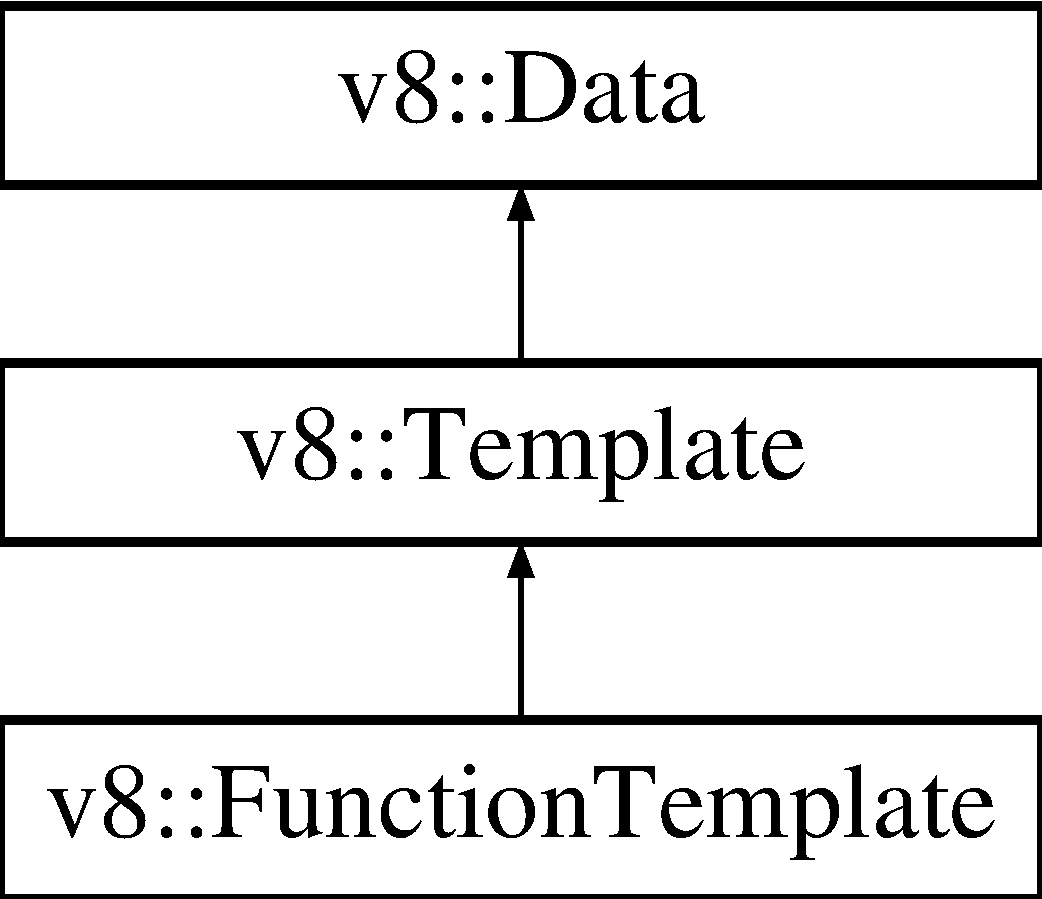
\includegraphics[height=3.000000cm]{classv8_1_1FunctionTemplate}
\end{center}
\end{figure}
\subsection*{Public Member Functions}
\begin{DoxyCompactItemize}
\item 
\hyperlink{classv8_1_1FunctionTemplate_a007fd05a3fa3c960bf7ddbc05c724d2b}{V8\+\_\+\+D\+E\+P\+R\+E\+C\+A\+T\+E\+\_\+\+S\+O\+O\+N} (\char`\"{}Use maybe version\char`\"{}, Local$<$ \hyperlink{classv8_1_1Function}{Function} $>$ Get\+Function())
\item 
\hypertarget{classv8_1_1FunctionTemplate_a77aa424e4ed297452be0412930340262}{}V8\+\_\+\+W\+A\+R\+N\+\_\+\+U\+N\+U\+S\+E\+D\+\_\+\+R\+E\+S\+U\+L\+T \hyperlink{classv8_1_1MaybeLocal}{Maybe\+Local}$<$ \hyperlink{classv8_1_1Function}{Function} $>$ {\bfseries Get\+Function} (\hyperlink{classv8_1_1Local}{Local}$<$ \hyperlink{classv8_1_1Context}{Context} $>$ context)\label{classv8_1_1FunctionTemplate_a77aa424e4ed297452be0412930340262}

\item 
void \hyperlink{classv8_1_1FunctionTemplate_a49babb7ea2d786a483a71514209455b6}{Set\+Call\+Handler} (Function\+Callback callback, \hyperlink{classv8_1_1Local}{Local}$<$ \hyperlink{classv8_1_1Value}{Value} $>$ data=\hyperlink{classv8_1_1Local}{Local}$<$ \hyperlink{classv8_1_1Value}{Value} $>$())
\item 
void \hyperlink{classv8_1_1FunctionTemplate_a5faf23b28ee3480b23ce054d0f389a75}{Set\+Length} (int length)
\item 
\hyperlink{classv8_1_1Local}{Local}$<$ \hyperlink{classv8_1_1ObjectTemplate}{Object\+Template} $>$ \hyperlink{classv8_1_1FunctionTemplate_a00dd9725566908e8fd14064542f5a781}{Instance\+Template} ()
\item 
void \hyperlink{classv8_1_1FunctionTemplate_abc11c462facf11bafd541892815c5425}{Inherit} (\hyperlink{classv8_1_1Local}{Local}$<$ \hyperlink{classv8_1_1FunctionTemplate}{Function\+Template} $>$ parent)
\item 
\hyperlink{classv8_1_1Local}{Local}$<$ \hyperlink{classv8_1_1ObjectTemplate}{Object\+Template} $>$ \hyperlink{classv8_1_1FunctionTemplate_aa2bcc2652b5f0fdbc666d943ccf72021}{Prototype\+Template} ()
\item 
void \hyperlink{classv8_1_1FunctionTemplate_a491e77dc7ceb5b0fe75880d11f2dbe9e}{Set\+Class\+Name} (\hyperlink{classv8_1_1Local}{Local}$<$ \hyperlink{classv8_1_1String}{String} $>$ name)
\item 
void \hyperlink{classv8_1_1FunctionTemplate_a5ffdc68d8035b02ed7583950b76ef91f}{Set\+Accept\+Any\+Receiver} (bool value)
\item 
void \hyperlink{classv8_1_1FunctionTemplate_ade426e8a21d777ae6100e6c1aa7bfaee}{Set\+Hidden\+Prototype} (bool value)
\item 
void \hyperlink{classv8_1_1FunctionTemplate_a91d2e0643e8c5a53ab1d75f7766c2422}{Read\+Only\+Prototype} ()
\item 
void \hyperlink{classv8_1_1FunctionTemplate_a4a184aca244174c7fe52d58871d3129e}{Remove\+Prototype} ()
\item 
bool \hyperlink{classv8_1_1FunctionTemplate_a90d838f3456d300bd19d2a2cb98645bd}{Has\+Instance} (\hyperlink{classv8_1_1Local}{Local}$<$ \hyperlink{classv8_1_1Value}{Value} $>$ object)
\end{DoxyCompactItemize}
\subsection*{Static Public Member Functions}
\begin{DoxyCompactItemize}
\item 
static \hyperlink{classv8_1_1Local}{Local}$<$ \hyperlink{classv8_1_1FunctionTemplate}{Function\+Template} $>$ \hyperlink{classv8_1_1FunctionTemplate_a3c6a525ee4e0d72afa77be8e34861f83}{New} (\hyperlink{classv8_1_1Isolate}{Isolate} $\ast$isolate, Function\+Callback callback=0, \hyperlink{classv8_1_1Local}{Local}$<$ \hyperlink{classv8_1_1Value}{Value} $>$ data=\hyperlink{classv8_1_1Local}{Local}$<$ \hyperlink{classv8_1_1Value}{Value} $>$(), \hyperlink{classv8_1_1Local}{Local}$<$ \hyperlink{classv8_1_1Signature}{Signature} $>$ signature=\hyperlink{classv8_1_1Local}{Local}$<$ \hyperlink{classv8_1_1Signature}{Signature} $>$(), int length=0)
\end{DoxyCompactItemize}
\subsection*{Friends}
\begin{DoxyCompactItemize}
\item 
\hypertarget{classv8_1_1FunctionTemplate_ac26c806e60ca4a0547680edb68f6e39b}{}class {\bfseries Context}\label{classv8_1_1FunctionTemplate_ac26c806e60ca4a0547680edb68f6e39b}

\item 
\hypertarget{classv8_1_1FunctionTemplate_a4d28646409234f556983be8a96c06424}{}class {\bfseries Object\+Template}\label{classv8_1_1FunctionTemplate_a4d28646409234f556983be8a96c06424}

\end{DoxyCompactItemize}


\subsection{Detailed Description}
A \hyperlink{classv8_1_1FunctionTemplate}{Function\+Template} is used to create functions at runtime. There can only be one function created from a \hyperlink{classv8_1_1FunctionTemplate}{Function\+Template} in a context. The lifetime of the created function is equal to the lifetime of the context. So in case the embedder needs to create temporary functions that can be collected using Scripts is preferred.

Any modification of a \hyperlink{classv8_1_1FunctionTemplate}{Function\+Template} after first instantiation will trigger a crash.

A \hyperlink{classv8_1_1FunctionTemplate}{Function\+Template} can have properties, these properties are added to the function object when it is created.

A \hyperlink{classv8_1_1FunctionTemplate}{Function\+Template} has a corresponding instance template which is used to create object instances when the function is used as a constructor. Properties added to the instance template are added to each object instance.

A \hyperlink{classv8_1_1FunctionTemplate}{Function\+Template} can have a prototype template. The prototype template is used to create the prototype object of the function.

The following example shows how to use a \hyperlink{classv8_1_1FunctionTemplate}{Function\+Template}\+:


\begin{DoxyCode}
\hyperlink{classv8_1_1Local}{v8::Local<v8::FunctionTemplate>} t = 
      \hyperlink{classv8_1_1FunctionTemplate_a3c6a525ee4e0d72afa77be8e34861f83}{v8::FunctionTemplate::New}();
t->\hyperlink{classv8_1_1Template_a623b9f0cdd87dc861516f276cc9a7cfa}{Set}(\textcolor{stringliteral}{"func\_property"}, v8::Number::New(1));

\hyperlink{classv8_1_1Local}{v8::Local<v8::Template>} proto\_t = t->\hyperlink{classv8_1_1FunctionTemplate_aa2bcc2652b5f0fdbc666d943ccf72021}{PrototypeTemplate}();
proto\_t->\hyperlink{classv8_1_1Template_a623b9f0cdd87dc861516f276cc9a7cfa}{Set}(\textcolor{stringliteral}{"proto\_method"}, \hyperlink{classv8_1_1FunctionTemplate_a3c6a525ee4e0d72afa77be8e34861f83}{v8::FunctionTemplate::New}(InvokeCallback));
proto\_t->\hyperlink{classv8_1_1Template_a623b9f0cdd87dc861516f276cc9a7cfa}{Set}(\textcolor{stringliteral}{"proto\_const"}, v8::Number::New(2));

\hyperlink{classv8_1_1Local}{v8::Local<v8::ObjectTemplate>} instance\_t = t->
      \hyperlink{classv8_1_1FunctionTemplate_a00dd9725566908e8fd14064542f5a781}{InstanceTemplate}();
instance\_t->\hyperlink{classv8_1_1ObjectTemplate_a7300126e15ff8246813e07f92d4fbe83}{SetAccessor}(\textcolor{stringliteral}{"instance\_accessor"}, InstanceAccessorCallback);
instance\_t->\hyperlink{classv8_1_1ObjectTemplate_a66fa7b04c87676e20e35497ea09a0ad0}{SetNamedPropertyHandler}(PropertyHandlerCallback, ...);
instance\_t->\hyperlink{classv8_1_1Template_a623b9f0cdd87dc861516f276cc9a7cfa}{Set}(\textcolor{stringliteral}{"instance\_property"}, Number::New(3));

\hyperlink{classv8_1_1Local}{v8::Local<v8::Function>} \textcolor{keyword}{function} = t->GetFunction();
\hyperlink{classv8_1_1Local}{v8::Local<v8::Object>} instance = \textcolor{keyword}{function}->NewInstance();
\end{DoxyCode}


Let\textquotesingle{}s use \char`\"{}function\char`\"{} as the J\+S variable name of the function object and \char`\"{}instance\char`\"{} for the instance object created above. The function and the instance will have the following properties\+:


\begin{DoxyCode}
func\_property in \textcolor{keyword}{function} == \textcolor{keyword}{true};
\textcolor{keyword}{function}.func\_property == 1;

\textcolor{keyword}{function}.prototype.proto\_method() invokes \textcolor{stringliteral}{'InvokeCallback'}
\textcolor{keyword}{function}.prototype.proto\_const == 2;

instance instanceof \textcolor{keyword}{function} == \textcolor{keyword}{true};
instance.instance\_accessor calls \textcolor{stringliteral}{'InstanceAccessorCallback'}
instance.instance\_property == 3;
\end{DoxyCode}


A \hyperlink{classv8_1_1FunctionTemplate}{Function\+Template} can inherit from another one by calling the \hyperlink{classv8_1_1FunctionTemplate_abc11c462facf11bafd541892815c5425}{Function\+Template\+::\+Inherit} method. The following graph illustrates the semantics of inheritance\+:


\begin{DoxyCode}
FunctionTemplate Parent  -> Parent() . prototype -> \{ \}
  ^                                                  ^
  | \hyperlink{classv8_1_1FunctionTemplate_abc11c462facf11bafd541892815c5425}{Inherit}(Parent)                                  | .\_\_proto\_\_
  |                                                  |
FunctionTemplate Child   -> Child()  . prototype -> \{ \}
\end{DoxyCode}


A \hyperlink{classv8_1_1FunctionTemplate}{Function\+Template} \textquotesingle{}Child\textquotesingle{} inherits from \textquotesingle{}Parent\textquotesingle{}, the prototype object of the Child() function has {\bfseries proto} pointing to the Parent() function\textquotesingle{}s prototype object. An instance of the Child function has all properties on Parent\textquotesingle{}s instance templates.

Let Parent be the \hyperlink{classv8_1_1FunctionTemplate}{Function\+Template} initialized in the previous section and create a Child \hyperlink{classv8_1_1FunctionTemplate}{Function\+Template} by\+:


\begin{DoxyCode}
Local<FunctionTemplate> parent = t;
Local<FunctionTemplate> child = \hyperlink{classv8_1_1FunctionTemplate_a3c6a525ee4e0d72afa77be8e34861f83}{FunctionTemplate::New}();
child->Inherit(parent);

Local<Function> child\_function = child->GetFunction();
Local<Object> child\_instance = child\_function->NewInstance();
\end{DoxyCode}


The Child function and Child instance will have the following properties\+:


\begin{DoxyCode}
child\_func.prototype.\_\_proto\_\_ == \textcolor{keyword}{function}.prototype;
child\_instance.instance\_accessor calls \textcolor{stringliteral}{'InstanceAccessorCallback'}
child\_instance.instance\_property == 3;
\end{DoxyCode}
 

\subsection{Member Function Documentation}
\hypertarget{classv8_1_1FunctionTemplate_a90d838f3456d300bd19d2a2cb98645bd}{}\index{v8\+::\+Function\+Template@{v8\+::\+Function\+Template}!Has\+Instance@{Has\+Instance}}
\index{Has\+Instance@{Has\+Instance}!v8\+::\+Function\+Template@{v8\+::\+Function\+Template}}
\subsubsection[{Has\+Instance}]{\setlength{\rightskip}{0pt plus 5cm}bool v8\+::\+Function\+Template\+::\+Has\+Instance (
\begin{DoxyParamCaption}
\item[{{\bf Local}$<$ {\bf Value} $>$}]{object}
\end{DoxyParamCaption}
)}\label{classv8_1_1FunctionTemplate_a90d838f3456d300bd19d2a2cb98645bd}
Returns true if the given object is an instance of this function template. \hypertarget{classv8_1_1FunctionTemplate_abc11c462facf11bafd541892815c5425}{}\index{v8\+::\+Function\+Template@{v8\+::\+Function\+Template}!Inherit@{Inherit}}
\index{Inherit@{Inherit}!v8\+::\+Function\+Template@{v8\+::\+Function\+Template}}
\subsubsection[{Inherit}]{\setlength{\rightskip}{0pt plus 5cm}void v8\+::\+Function\+Template\+::\+Inherit (
\begin{DoxyParamCaption}
\item[{{\bf Local}$<$ {\bf Function\+Template} $>$}]{parent}
\end{DoxyParamCaption}
)}\label{classv8_1_1FunctionTemplate_abc11c462facf11bafd541892815c5425}
Causes the function template to inherit from a parent function template. \hypertarget{classv8_1_1FunctionTemplate_a00dd9725566908e8fd14064542f5a781}{}\index{v8\+::\+Function\+Template@{v8\+::\+Function\+Template}!Instance\+Template@{Instance\+Template}}
\index{Instance\+Template@{Instance\+Template}!v8\+::\+Function\+Template@{v8\+::\+Function\+Template}}
\subsubsection[{Instance\+Template}]{\setlength{\rightskip}{0pt plus 5cm}{\bf Local}$<${\bf Object\+Template}$>$ v8\+::\+Function\+Template\+::\+Instance\+Template (
\begin{DoxyParamCaption}
{}
\end{DoxyParamCaption}
)}\label{classv8_1_1FunctionTemplate_a00dd9725566908e8fd14064542f5a781}
Get the Instance\+Template. \hypertarget{classv8_1_1FunctionTemplate_a3c6a525ee4e0d72afa77be8e34861f83}{}\index{v8\+::\+Function\+Template@{v8\+::\+Function\+Template}!New@{New}}
\index{New@{New}!v8\+::\+Function\+Template@{v8\+::\+Function\+Template}}
\subsubsection[{New}]{\setlength{\rightskip}{0pt plus 5cm}static {\bf Local}$<${\bf Function\+Template}$>$ v8\+::\+Function\+Template\+::\+New (
\begin{DoxyParamCaption}
\item[{{\bf Isolate} $\ast$}]{isolate, }
\item[{Function\+Callback}]{callback = {\ttfamily 0}, }
\item[{{\bf Local}$<$ {\bf Value} $>$}]{data = {\ttfamily {\bf Local}$<$~{\bf Value}~$>$()}, }
\item[{{\bf Local}$<$ {\bf Signature} $>$}]{signature = {\ttfamily {\bf Local}$<$~{\bf Signature}~$>$()}, }
\item[{int}]{length = {\ttfamily 0}}
\end{DoxyParamCaption}
)\hspace{0.3cm}{\ttfamily [static]}}\label{classv8_1_1FunctionTemplate_a3c6a525ee4e0d72afa77be8e34861f83}
Creates a function template. \hypertarget{classv8_1_1FunctionTemplate_aa2bcc2652b5f0fdbc666d943ccf72021}{}\index{v8\+::\+Function\+Template@{v8\+::\+Function\+Template}!Prototype\+Template@{Prototype\+Template}}
\index{Prototype\+Template@{Prototype\+Template}!v8\+::\+Function\+Template@{v8\+::\+Function\+Template}}
\subsubsection[{Prototype\+Template}]{\setlength{\rightskip}{0pt plus 5cm}{\bf Local}$<${\bf Object\+Template}$>$ v8\+::\+Function\+Template\+::\+Prototype\+Template (
\begin{DoxyParamCaption}
{}
\end{DoxyParamCaption}
)}\label{classv8_1_1FunctionTemplate_aa2bcc2652b5f0fdbc666d943ccf72021}
A Prototype\+Template is the template used to create the prototype object of the function created by this template. \hypertarget{classv8_1_1FunctionTemplate_a91d2e0643e8c5a53ab1d75f7766c2422}{}\index{v8\+::\+Function\+Template@{v8\+::\+Function\+Template}!Read\+Only\+Prototype@{Read\+Only\+Prototype}}
\index{Read\+Only\+Prototype@{Read\+Only\+Prototype}!v8\+::\+Function\+Template@{v8\+::\+Function\+Template}}
\subsubsection[{Read\+Only\+Prototype}]{\setlength{\rightskip}{0pt plus 5cm}void v8\+::\+Function\+Template\+::\+Read\+Only\+Prototype (
\begin{DoxyParamCaption}
{}
\end{DoxyParamCaption}
)}\label{classv8_1_1FunctionTemplate_a91d2e0643e8c5a53ab1d75f7766c2422}
Sets the Read\+Only flag in the attributes of the \textquotesingle{}prototype\textquotesingle{} property of functions created from this \hyperlink{classv8_1_1FunctionTemplate}{Function\+Template} to true. \hypertarget{classv8_1_1FunctionTemplate_a4a184aca244174c7fe52d58871d3129e}{}\index{v8\+::\+Function\+Template@{v8\+::\+Function\+Template}!Remove\+Prototype@{Remove\+Prototype}}
\index{Remove\+Prototype@{Remove\+Prototype}!v8\+::\+Function\+Template@{v8\+::\+Function\+Template}}
\subsubsection[{Remove\+Prototype}]{\setlength{\rightskip}{0pt plus 5cm}void v8\+::\+Function\+Template\+::\+Remove\+Prototype (
\begin{DoxyParamCaption}
{}
\end{DoxyParamCaption}
)}\label{classv8_1_1FunctionTemplate_a4a184aca244174c7fe52d58871d3129e}
Removes the prototype property from functions created from this \hyperlink{classv8_1_1FunctionTemplate}{Function\+Template}. \hypertarget{classv8_1_1FunctionTemplate_a5ffdc68d8035b02ed7583950b76ef91f}{}\index{v8\+::\+Function\+Template@{v8\+::\+Function\+Template}!Set\+Accept\+Any\+Receiver@{Set\+Accept\+Any\+Receiver}}
\index{Set\+Accept\+Any\+Receiver@{Set\+Accept\+Any\+Receiver}!v8\+::\+Function\+Template@{v8\+::\+Function\+Template}}
\subsubsection[{Set\+Accept\+Any\+Receiver}]{\setlength{\rightskip}{0pt plus 5cm}void v8\+::\+Function\+Template\+::\+Set\+Accept\+Any\+Receiver (
\begin{DoxyParamCaption}
\item[{bool}]{value}
\end{DoxyParamCaption}
)}\label{classv8_1_1FunctionTemplate_a5ffdc68d8035b02ed7583950b76ef91f}
When set to true, no access check will be performed on the receiver of a function call. Currently defaults to true, but this is subject to change. \hypertarget{classv8_1_1FunctionTemplate_a49babb7ea2d786a483a71514209455b6}{}\index{v8\+::\+Function\+Template@{v8\+::\+Function\+Template}!Set\+Call\+Handler@{Set\+Call\+Handler}}
\index{Set\+Call\+Handler@{Set\+Call\+Handler}!v8\+::\+Function\+Template@{v8\+::\+Function\+Template}}
\subsubsection[{Set\+Call\+Handler}]{\setlength{\rightskip}{0pt plus 5cm}void v8\+::\+Function\+Template\+::\+Set\+Call\+Handler (
\begin{DoxyParamCaption}
\item[{Function\+Callback}]{callback, }
\item[{{\bf Local}$<$ {\bf Value} $>$}]{data = {\ttfamily {\bf Local}$<$~{\bf Value}~$>$()}}
\end{DoxyParamCaption}
)}\label{classv8_1_1FunctionTemplate_a49babb7ea2d786a483a71514209455b6}
\hyperlink{classv8_1_1Set}{Set} the call-\/handler callback for a \hyperlink{classv8_1_1FunctionTemplate}{Function\+Template}. This callback is called whenever the function created from this \hyperlink{classv8_1_1FunctionTemplate}{Function\+Template} is called. \hypertarget{classv8_1_1FunctionTemplate_a491e77dc7ceb5b0fe75880d11f2dbe9e}{}\index{v8\+::\+Function\+Template@{v8\+::\+Function\+Template}!Set\+Class\+Name@{Set\+Class\+Name}}
\index{Set\+Class\+Name@{Set\+Class\+Name}!v8\+::\+Function\+Template@{v8\+::\+Function\+Template}}
\subsubsection[{Set\+Class\+Name}]{\setlength{\rightskip}{0pt plus 5cm}void v8\+::\+Function\+Template\+::\+Set\+Class\+Name (
\begin{DoxyParamCaption}
\item[{{\bf Local}$<$ {\bf String} $>$}]{name}
\end{DoxyParamCaption}
)}\label{classv8_1_1FunctionTemplate_a491e77dc7ceb5b0fe75880d11f2dbe9e}
\hyperlink{classv8_1_1Set}{Set} the class name of the \hyperlink{classv8_1_1FunctionTemplate}{Function\+Template}. This is used for printing objects created with the function created from the \hyperlink{classv8_1_1FunctionTemplate}{Function\+Template} as its constructor. \hypertarget{classv8_1_1FunctionTemplate_ade426e8a21d777ae6100e6c1aa7bfaee}{}\index{v8\+::\+Function\+Template@{v8\+::\+Function\+Template}!Set\+Hidden\+Prototype@{Set\+Hidden\+Prototype}}
\index{Set\+Hidden\+Prototype@{Set\+Hidden\+Prototype}!v8\+::\+Function\+Template@{v8\+::\+Function\+Template}}
\subsubsection[{Set\+Hidden\+Prototype}]{\setlength{\rightskip}{0pt plus 5cm}void v8\+::\+Function\+Template\+::\+Set\+Hidden\+Prototype (
\begin{DoxyParamCaption}
\item[{bool}]{value}
\end{DoxyParamCaption}
)}\label{classv8_1_1FunctionTemplate_ade426e8a21d777ae6100e6c1aa7bfaee}
Determines whether the {\bfseries proto} accessor ignores instances of the function template. If instances of the function template are ignored, {\bfseries proto} skips all instances and instead returns the next object in the prototype chain.

Call with a value of true to make the {\bfseries proto} accessor ignore instances of the function template. Call with a value of false to make the {\bfseries proto} accessor not ignore instances of the function template. By default, instances of a function template are not ignored. \hypertarget{classv8_1_1FunctionTemplate_a5faf23b28ee3480b23ce054d0f389a75}{}\index{v8\+::\+Function\+Template@{v8\+::\+Function\+Template}!Set\+Length@{Set\+Length}}
\index{Set\+Length@{Set\+Length}!v8\+::\+Function\+Template@{v8\+::\+Function\+Template}}
\subsubsection[{Set\+Length}]{\setlength{\rightskip}{0pt plus 5cm}void v8\+::\+Function\+Template\+::\+Set\+Length (
\begin{DoxyParamCaption}
\item[{int}]{length}
\end{DoxyParamCaption}
)}\label{classv8_1_1FunctionTemplate_a5faf23b28ee3480b23ce054d0f389a75}
\hyperlink{classv8_1_1Set}{Set} the predefined length property for the \hyperlink{classv8_1_1FunctionTemplate}{Function\+Template}. \hypertarget{classv8_1_1FunctionTemplate_a007fd05a3fa3c960bf7ddbc05c724d2b}{}\index{v8\+::\+Function\+Template@{v8\+::\+Function\+Template}!V8\+\_\+\+D\+E\+P\+R\+E\+C\+A\+T\+E\+\_\+\+S\+O\+O\+N@{V8\+\_\+\+D\+E\+P\+R\+E\+C\+A\+T\+E\+\_\+\+S\+O\+O\+N}}
\index{V8\+\_\+\+D\+E\+P\+R\+E\+C\+A\+T\+E\+\_\+\+S\+O\+O\+N@{V8\+\_\+\+D\+E\+P\+R\+E\+C\+A\+T\+E\+\_\+\+S\+O\+O\+N}!v8\+::\+Function\+Template@{v8\+::\+Function\+Template}}
\subsubsection[{V8\+\_\+\+D\+E\+P\+R\+E\+C\+A\+T\+E\+\_\+\+S\+O\+O\+N}]{\setlength{\rightskip}{0pt plus 5cm}v8\+::\+Function\+Template\+::\+V8\+\_\+\+D\+E\+P\+R\+E\+C\+A\+T\+E\+\_\+\+S\+O\+O\+N (
\begin{DoxyParamCaption}
\item[{\char`\"{}Use maybe version\char`\"{}}]{, }
\item[{{\bf Local}$<$ {\bf Function} $>$ }]{Get\+Function()}
\end{DoxyParamCaption}
)}\label{classv8_1_1FunctionTemplate_a007fd05a3fa3c960bf7ddbc05c724d2b}
Returns the unique function instance in the current execution context. 

The documentation for this class was generated from the following file\+:\begin{DoxyCompactItemize}
\item 
v8/include/v8.\+h\end{DoxyCompactItemize}

\hypertarget{classv8_1_1Global}{}\section{v8\+:\+:Global$<$ T $>$ Class Template Reference}
\label{classv8_1_1Global}\index{v8\+::\+Global$<$ T $>$@{v8\+::\+Global$<$ T $>$}}


{\ttfamily \#include $<$v8.\+h$>$}

Inheritance diagram for v8\+:\+:Global$<$ T $>$\+:\begin{figure}[H]
\begin{center}
\leavevmode
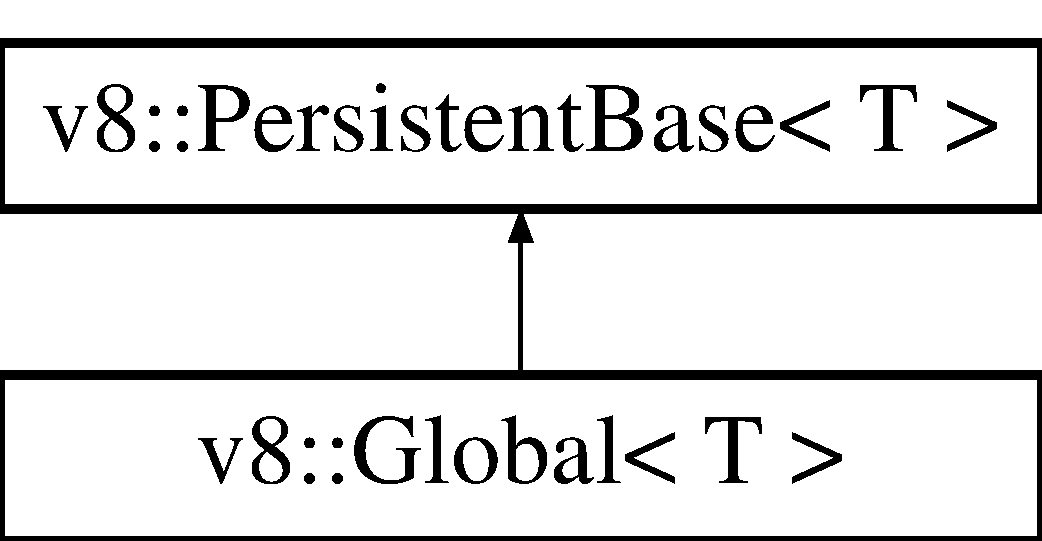
\includegraphics[height=2.000000cm]{classv8_1_1Global}
\end{center}
\end{figure}
\subsection*{Public Types}
\begin{DoxyCompactItemize}
\item 
\hypertarget{classv8_1_1Global_a295826e79781fe585904e652884db72f}{}typedef void {\bfseries Move\+Only\+Type\+For\+C\+P\+P03}\label{classv8_1_1Global_a295826e79781fe585904e652884db72f}

\end{DoxyCompactItemize}
\subsection*{Public Member Functions}
\begin{DoxyCompactItemize}
\item 
V8\+\_\+\+I\+N\+L\+I\+N\+E \hyperlink{classv8_1_1Global_ab1efdf25ff6305e67f3266a6fe90527e}{Global} ()
\item 
{\footnotesize template$<$class S $>$ }\\V8\+\_\+\+I\+N\+L\+I\+N\+E \hyperlink{classv8_1_1Global_a8434bb6729eb4cd0cd85ad81bd8344ad}{Global} (\hyperlink{classv8_1_1Isolate}{Isolate} $\ast$isolate, \hyperlink{classv8_1_1Local}{Local}$<$ S $>$ that)
\item 
{\footnotesize template$<$class S $>$ }\\V8\+\_\+\+I\+N\+L\+I\+N\+E \hyperlink{classv8_1_1Global_a6243ecb28bb97d066065796fa28f7415}{Global} (\hyperlink{classv8_1_1Isolate}{Isolate} $\ast$isolate, const \hyperlink{classv8_1_1PersistentBase}{Persistent\+Base}$<$ S $>$ \&that)
\item 
V8\+\_\+\+I\+N\+L\+I\+N\+E \hyperlink{classv8_1_1Global_ab8f3c754a58146e6db67012cd74a49cb}{Global} (\hyperlink{classv8_1_1Global}{Global} \&\&other)
\item 
{\footnotesize template$<$class S $>$ }\\V8\+\_\+\+I\+N\+L\+I\+N\+E \hyperlink{classv8_1_1Global}{Global} \& \hyperlink{classv8_1_1Global_a9d3d7d8f10ad23e413f2027cc15ab209}{operator=} (\hyperlink{classv8_1_1Global}{Global}$<$ S $>$ \&\&rhs)
\item 
\hyperlink{classv8_1_1Global}{Global} \hyperlink{classv8_1_1Global_a914903149cc752468d4a3a11b6089c7e}{Pass} ()
\end{DoxyCompactItemize}
\subsection*{Friends}
\begin{DoxyCompactItemize}
\item 
\hypertarget{classv8_1_1Global_a53f604d3d6f2dc0647df33c9979f116a}{}{\footnotesize template$<$class F $>$ }\\class {\bfseries Return\+Value}\label{classv8_1_1Global_a53f604d3d6f2dc0647df33c9979f116a}

\end{DoxyCompactItemize}


\subsection{Detailed Description}
\subsubsection*{template$<$class T$>$class v8\+::\+Global$<$ T $>$}

A \hyperlink{classv8_1_1PersistentBase}{Persistent\+Base} which has move semantics.

Note\+: \hyperlink{classv8_1_1Persistent}{Persistent} class hierarchy is subject to future changes. 

\subsection{Constructor \& Destructor Documentation}
\hypertarget{classv8_1_1Global_ab1efdf25ff6305e67f3266a6fe90527e}{}\index{v8\+::\+Global@{v8\+::\+Global}!Global@{Global}}
\index{Global@{Global}!v8\+::\+Global@{v8\+::\+Global}}
\subsubsection[{Global}]{\setlength{\rightskip}{0pt plus 5cm}template$<$class T$>$ V8\+\_\+\+I\+N\+L\+I\+N\+E {\bf v8\+::\+Global}$<$ T $>$\+::{\bf Global} (
\begin{DoxyParamCaption}
{}
\end{DoxyParamCaption}
)\hspace{0.3cm}{\ttfamily [inline]}}\label{classv8_1_1Global_ab1efdf25ff6305e67f3266a6fe90527e}
A \hyperlink{classv8_1_1Global}{Global} with no storage cell. \hypertarget{classv8_1_1Global_a8434bb6729eb4cd0cd85ad81bd8344ad}{}\index{v8\+::\+Global@{v8\+::\+Global}!Global@{Global}}
\index{Global@{Global}!v8\+::\+Global@{v8\+::\+Global}}
\subsubsection[{Global}]{\setlength{\rightskip}{0pt plus 5cm}template$<$class T$>$ template$<$class S $>$ V8\+\_\+\+I\+N\+L\+I\+N\+E {\bf v8\+::\+Global}$<$ T $>$\+::{\bf Global} (
\begin{DoxyParamCaption}
\item[{{\bf Isolate} $\ast$}]{isolate, }
\item[{{\bf Local}$<$ S $>$}]{that}
\end{DoxyParamCaption}
)\hspace{0.3cm}{\ttfamily [inline]}}\label{classv8_1_1Global_a8434bb6729eb4cd0cd85ad81bd8344ad}
Construct a \hyperlink{classv8_1_1Global}{Global} from a \hyperlink{classv8_1_1Local}{Local}. When the \hyperlink{classv8_1_1Local}{Local} is non-\/empty, a new storage cell is created pointing to the same object, and no flags are set. \hypertarget{classv8_1_1Global_a6243ecb28bb97d066065796fa28f7415}{}\index{v8\+::\+Global@{v8\+::\+Global}!Global@{Global}}
\index{Global@{Global}!v8\+::\+Global@{v8\+::\+Global}}
\subsubsection[{Global}]{\setlength{\rightskip}{0pt plus 5cm}template$<$class T$>$ template$<$class S $>$ V8\+\_\+\+I\+N\+L\+I\+N\+E {\bf v8\+::\+Global}$<$ T $>$\+::{\bf Global} (
\begin{DoxyParamCaption}
\item[{{\bf Isolate} $\ast$}]{isolate, }
\item[{const {\bf Persistent\+Base}$<$ S $>$ \&}]{that}
\end{DoxyParamCaption}
)\hspace{0.3cm}{\ttfamily [inline]}}\label{classv8_1_1Global_a6243ecb28bb97d066065796fa28f7415}
Construct a \hyperlink{classv8_1_1Global}{Global} from a \hyperlink{classv8_1_1PersistentBase}{Persistent\+Base}. When the \hyperlink{classv8_1_1Persistent}{Persistent} is non-\/empty, a new storage cell is created pointing to the same object, and no flags are set. \hypertarget{classv8_1_1Global_ab8f3c754a58146e6db67012cd74a49cb}{}\index{v8\+::\+Global@{v8\+::\+Global}!Global@{Global}}
\index{Global@{Global}!v8\+::\+Global@{v8\+::\+Global}}
\subsubsection[{Global}]{\setlength{\rightskip}{0pt plus 5cm}template$<$class T$>$ V8\+\_\+\+I\+N\+L\+I\+N\+E {\bf v8\+::\+Global}$<$ T $>$\+::{\bf Global} (
\begin{DoxyParamCaption}
\item[{{\bf Global}$<$ T $>$ \&\&}]{other}
\end{DoxyParamCaption}
)\hspace{0.3cm}{\ttfamily [inline]}}\label{classv8_1_1Global_ab8f3c754a58146e6db67012cd74a49cb}
Move constructor. 

\subsection{Member Function Documentation}
\hypertarget{classv8_1_1Global_a9d3d7d8f10ad23e413f2027cc15ab209}{}\index{v8\+::\+Global@{v8\+::\+Global}!operator=@{operator=}}
\index{operator=@{operator=}!v8\+::\+Global@{v8\+::\+Global}}
\subsubsection[{operator=}]{\setlength{\rightskip}{0pt plus 5cm}template$<$class T$>$ template$<$class S $>$ V8\+\_\+\+I\+N\+L\+I\+N\+E {\bf Global}\& {\bf v8\+::\+Global}$<$ T $>$\+::operator= (
\begin{DoxyParamCaption}
\item[{{\bf Global}$<$ S $>$ \&\&}]{rhs}
\end{DoxyParamCaption}
)\hspace{0.3cm}{\ttfamily [inline]}}\label{classv8_1_1Global_a9d3d7d8f10ad23e413f2027cc15ab209}
Move via assignment. \hypertarget{classv8_1_1Global_a914903149cc752468d4a3a11b6089c7e}{}\index{v8\+::\+Global@{v8\+::\+Global}!Pass@{Pass}}
\index{Pass@{Pass}!v8\+::\+Global@{v8\+::\+Global}}
\subsubsection[{Pass}]{\setlength{\rightskip}{0pt plus 5cm}template$<$class T$>$ {\bf Global} {\bf v8\+::\+Global}$<$ T $>$\+::Pass (
\begin{DoxyParamCaption}
{}
\end{DoxyParamCaption}
)\hspace{0.3cm}{\ttfamily [inline]}}\label{classv8_1_1Global_a914903149cc752468d4a3a11b6089c7e}
Pass allows returning uniques from functions, etc. 

The documentation for this class was generated from the following file\+:\begin{DoxyCompactItemize}
\item 
v8/include/v8.\+h\end{DoxyCompactItemize}

\hypertarget{classv8_1_1GlobalValueMap}{}\section{v8\+:\+:Global\+Value\+Map$<$ K, V, Traits $>$ Class Template Reference}
\label{classv8_1_1GlobalValueMap}\index{v8\+::\+Global\+Value\+Map$<$ K, V, Traits $>$@{v8\+::\+Global\+Value\+Map$<$ K, V, Traits $>$}}
Inheritance diagram for v8\+:\+:Global\+Value\+Map$<$ K, V, Traits $>$\+:\begin{figure}[H]
\begin{center}
\leavevmode
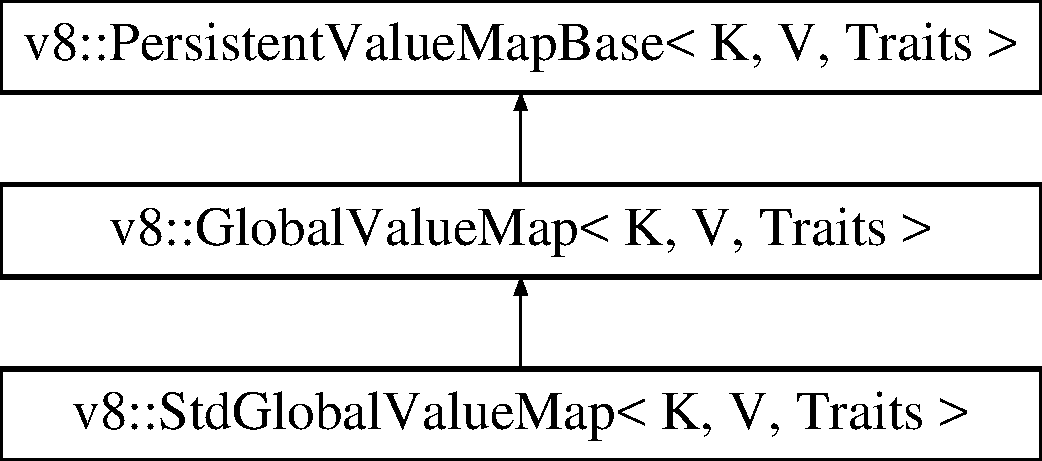
\includegraphics[height=3.000000cm]{classv8_1_1GlobalValueMap}
\end{center}
\end{figure}
\subsection*{Public Types}
\begin{DoxyCompactItemize}
\item 
\hypertarget{classv8_1_1GlobalValueMap_ac01835ce1863e1c577882e31b60efc35}{}typedef \hyperlink{classv8_1_1PersistentValueMapBase}{Persistent\+Value\+Map\+Base}$<$ K, V, Traits $>$\+::\hyperlink{classv8_1_1PersistentValueMapBase_1_1PersistentValueReference}{Persistent\+Value\+Reference} {\bfseries Persistent\+Value\+Reference}\label{classv8_1_1GlobalValueMap_ac01835ce1863e1c577882e31b60efc35}

\end{DoxyCompactItemize}
\subsection*{Public Member Functions}
\begin{DoxyCompactItemize}
\item 
\hypertarget{classv8_1_1GlobalValueMap_a60018c72fdae03d51b687d2a941140f4}{}{\bfseries Global\+Value\+Map} (\hyperlink{classv8_1_1Isolate}{Isolate} $\ast$isolate)\label{classv8_1_1GlobalValueMap_a60018c72fdae03d51b687d2a941140f4}

\item 
\hyperlink{classv8_1_1Global}{Global}$<$ V $>$ \hyperlink{classv8_1_1GlobalValueMap_aa13f7914642c705b8e96824747ea115a}{Set} (const K \&key, \hyperlink{classv8_1_1Local}{Local}$<$ V $>$ value)
\item 
\hyperlink{classv8_1_1Global}{Global}$<$ V $>$ \hyperlink{classv8_1_1GlobalValueMap_ac2b02a0105393e6e3ab7e0aeeed9a294}{Set} (const K \&key, \hyperlink{classv8_1_1Global}{Global}$<$ V $>$ value)
\item 
\hyperlink{classv8_1_1Global}{Global}$<$ V $>$ \hyperlink{classv8_1_1GlobalValueMap_aad73de3912571a2f245454d3edea4a41}{Set\+Unique} (const K \&key, \hyperlink{classv8_1_1Global}{Global}$<$ V $>$ $\ast$persistent)
\item 
\hyperlink{classv8_1_1Global}{Global}$<$ V $>$ \hyperlink{classv8_1_1GlobalValueMap_aaa5fa26f751c8608716ad5578cd6c1d0}{Set} (const K \&key, \hyperlink{classv8_1_1Global}{Global}$<$ V $>$ value, \hyperlink{classv8_1_1PersistentValueMapBase_1_1PersistentValueReference}{Persistent\+Value\+Reference} $\ast$reference)
\end{DoxyCompactItemize}
\subsection*{Additional Inherited Members}


\subsection{Member Function Documentation}
\hypertarget{classv8_1_1GlobalValueMap_aa13f7914642c705b8e96824747ea115a}{}\index{v8\+::\+Global\+Value\+Map@{v8\+::\+Global\+Value\+Map}!Set@{Set}}
\index{Set@{Set}!v8\+::\+Global\+Value\+Map@{v8\+::\+Global\+Value\+Map}}
\subsubsection[{Set}]{\setlength{\rightskip}{0pt plus 5cm}template$<$typename K , typename V , typename Traits $>$ {\bf Global}$<$V$>$ {\bf v8\+::\+Global\+Value\+Map}$<$ K, V, Traits $>$\+::{\bf Set} (
\begin{DoxyParamCaption}
\item[{const K \&}]{key, }
\item[{{\bf Local}$<$ V $>$}]{value}
\end{DoxyParamCaption}
)\hspace{0.3cm}{\ttfamily [inline]}}\label{classv8_1_1GlobalValueMap_aa13f7914642c705b8e96824747ea115a}
Put value into map. Depending on Traits\+::k\+Is\+Weak, the value will be held by the map strongly or weakly. Returns old value as \hyperlink{classv8_1_1Global}{Global}. \hypertarget{classv8_1_1GlobalValueMap_ac2b02a0105393e6e3ab7e0aeeed9a294}{}\index{v8\+::\+Global\+Value\+Map@{v8\+::\+Global\+Value\+Map}!Set@{Set}}
\index{Set@{Set}!v8\+::\+Global\+Value\+Map@{v8\+::\+Global\+Value\+Map}}
\subsubsection[{Set}]{\setlength{\rightskip}{0pt plus 5cm}template$<$typename K , typename V , typename Traits $>$ {\bf Global}$<$V$>$ {\bf v8\+::\+Global\+Value\+Map}$<$ K, V, Traits $>$\+::{\bf Set} (
\begin{DoxyParamCaption}
\item[{const K \&}]{key, }
\item[{{\bf Global}$<$ V $>$}]{value}
\end{DoxyParamCaption}
)\hspace{0.3cm}{\ttfamily [inline]}}\label{classv8_1_1GlobalValueMap_ac2b02a0105393e6e3ab7e0aeeed9a294}
Put value into map, like \hyperlink{classv8_1_1GlobalValueMap_aa13f7914642c705b8e96824747ea115a}{Set(const K\&, Local$<$\+V$>$)}. \hypertarget{classv8_1_1GlobalValueMap_aaa5fa26f751c8608716ad5578cd6c1d0}{}\index{v8\+::\+Global\+Value\+Map@{v8\+::\+Global\+Value\+Map}!Set@{Set}}
\index{Set@{Set}!v8\+::\+Global\+Value\+Map@{v8\+::\+Global\+Value\+Map}}
\subsubsection[{Set}]{\setlength{\rightskip}{0pt plus 5cm}template$<$typename K , typename V , typename Traits $>$ {\bf Global}$<$V$>$ {\bf v8\+::\+Global\+Value\+Map}$<$ K, V, Traits $>$\+::{\bf Set} (
\begin{DoxyParamCaption}
\item[{const K \&}]{key, }
\item[{{\bf Global}$<$ V $>$}]{value, }
\item[{{\bf Persistent\+Value\+Reference} $\ast$}]{reference}
\end{DoxyParamCaption}
)\hspace{0.3cm}{\ttfamily [inline]}}\label{classv8_1_1GlobalValueMap_aaa5fa26f751c8608716ad5578cd6c1d0}
Put a value into the map and update the reference. Restrictions of Get\+Reference apply here as well. \hypertarget{classv8_1_1GlobalValueMap_aad73de3912571a2f245454d3edea4a41}{}\index{v8\+::\+Global\+Value\+Map@{v8\+::\+Global\+Value\+Map}!Set\+Unique@{Set\+Unique}}
\index{Set\+Unique@{Set\+Unique}!v8\+::\+Global\+Value\+Map@{v8\+::\+Global\+Value\+Map}}
\subsubsection[{Set\+Unique}]{\setlength{\rightskip}{0pt plus 5cm}template$<$typename K , typename V , typename Traits $>$ {\bf Global}$<$V$>$ {\bf v8\+::\+Global\+Value\+Map}$<$ K, V, Traits $>$\+::Set\+Unique (
\begin{DoxyParamCaption}
\item[{const K \&}]{key, }
\item[{{\bf Global}$<$ V $>$ $\ast$}]{persistent}
\end{DoxyParamCaption}
)\hspace{0.3cm}{\ttfamily [inline]}}\label{classv8_1_1GlobalValueMap_aad73de3912571a2f245454d3edea4a41}
Put the value into the map, and set the \textquotesingle{}weak\textquotesingle{} callback when demanded by the Traits class. 

The documentation for this class was generated from the following file\+:\begin{DoxyCompactItemize}
\item 
v8/include/v8-\/util.\+h\end{DoxyCompactItemize}

\hypertarget{classv8_1_1HandleScope}{}\section{v8\+:\+:Handle\+Scope Class Reference}
\label{classv8_1_1HandleScope}\index{v8\+::\+Handle\+Scope@{v8\+::\+Handle\+Scope}}


{\ttfamily \#include $<$v8.\+h$>$}

Inheritance diagram for v8\+:\+:Handle\+Scope\+:\begin{figure}[H]
\begin{center}
\leavevmode
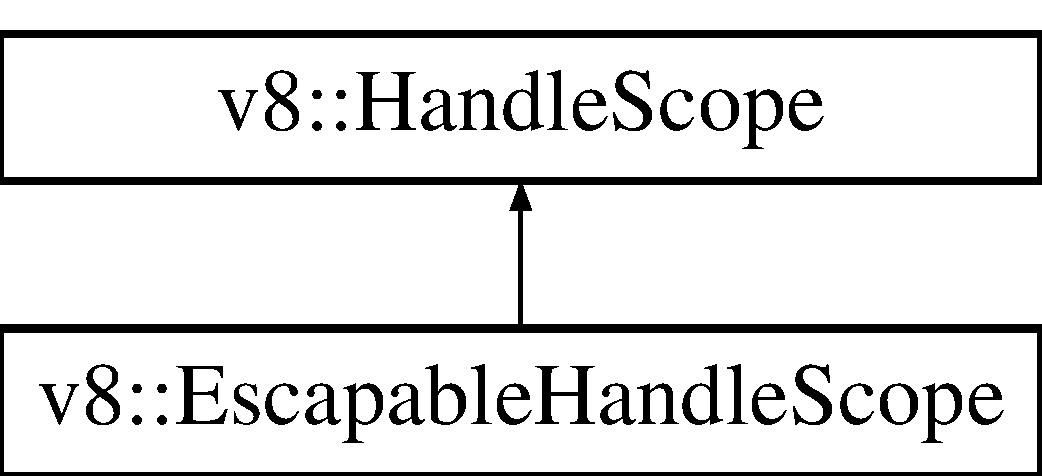
\includegraphics[height=2.000000cm]{classv8_1_1HandleScope}
\end{center}
\end{figure}
\subsection*{Public Member Functions}
\begin{DoxyCompactItemize}
\item 
\mbox{\Hypertarget{classv8_1_1HandleScope_afdb3053d852ea467f026b025ed431e79}\label{classv8_1_1HandleScope_afdb3053d852ea467f026b025ed431e79}} 
{\bfseries Handle\+Scope} (Isolate $\ast$isolate)
\item 
\mbox{\Hypertarget{classv8_1_1HandleScope_ad605be00a8f9bfd8157806102af95fab}\label{classv8_1_1HandleScope_ad605be00a8f9bfd8157806102af95fab}} 
V8\+\_\+\+I\+N\+L\+I\+NE Isolate $\ast$ {\bfseries Get\+Isolate} () const
\item 
\mbox{\Hypertarget{classv8_1_1HandleScope_a8354f068f3185cb663ecb689587fbbe8}\label{classv8_1_1HandleScope_a8354f068f3185cb663ecb689587fbbe8}} 
{\bfseries Handle\+Scope} (const \mbox{\hyperlink{classv8_1_1HandleScope}{Handle\+Scope}} \&)=delete
\item 
\mbox{\Hypertarget{classv8_1_1HandleScope_a6570b4a527ee30057026a15f3ebe62b2}\label{classv8_1_1HandleScope_a6570b4a527ee30057026a15f3ebe62b2}} 
void {\bfseries operator=} (const \mbox{\hyperlink{classv8_1_1HandleScope}{Handle\+Scope}} \&)=delete
\end{DoxyCompactItemize}
\subsection*{Static Public Member Functions}
\begin{DoxyCompactItemize}
\item 
static int \mbox{\hyperlink{classv8_1_1HandleScope_abab7214c9b9388b02f575fd5270b7e2f}{Number\+Of\+Handles}} (Isolate $\ast$isolate)
\end{DoxyCompactItemize}
\subsection*{Protected Member Functions}
\begin{DoxyCompactItemize}
\item 
\mbox{\Hypertarget{classv8_1_1HandleScope_a7bb8631c1c8756b05e9232b8414dd992}\label{classv8_1_1HandleScope_a7bb8631c1c8756b05e9232b8414dd992}} 
void {\bfseries Initialize} (Isolate $\ast$isolate)
\end{DoxyCompactItemize}
\subsection*{Static Protected Member Functions}
\begin{DoxyCompactItemize}
\item 
\mbox{\Hypertarget{classv8_1_1HandleScope_a1dfeb02024b2b75746a1aa1f0b2e94fa}\label{classv8_1_1HandleScope_a1dfeb02024b2b75746a1aa1f0b2e94fa}} 
static internal\+::\+Address $\ast$ {\bfseries Create\+Handle} (internal\+::\+Isolate $\ast$isolate, internal\+::\+Address value)
\end{DoxyCompactItemize}
\subsection*{Friends}
\begin{DoxyCompactItemize}
\item 
\mbox{\Hypertarget{classv8_1_1HandleScope_afb872edb4aac7ba55f0da004113aa2b0}\label{classv8_1_1HandleScope_afb872edb4aac7ba55f0da004113aa2b0}} 
{\footnotesize template$<$class F $>$ }\\class {\bfseries Local}
\item 
\mbox{\Hypertarget{classv8_1_1HandleScope_a0720b5f434e636e22a3ed34f847eec57}\label{classv8_1_1HandleScope_a0720b5f434e636e22a3ed34f847eec57}} 
class {\bfseries Object}
\item 
\mbox{\Hypertarget{classv8_1_1HandleScope_ac26c806e60ca4a0547680edb68f6e39b}\label{classv8_1_1HandleScope_ac26c806e60ca4a0547680edb68f6e39b}} 
class {\bfseries Context}
\end{DoxyCompactItemize}


\subsection{Detailed Description}
A stack-\/allocated class that governs a number of local handles. After a handle scope has been created, all local handles will be allocated within that handle scope until either the handle scope is deleted or another handle scope is created. If there is already a handle scope and a new one is created, all allocations will take place in the new handle scope until it is deleted. After that, new handles will again be allocated in the original handle scope.

After the handle scope of a local handle has been deleted the garbage collector will no longer track the object stored in the handle and may deallocate it. The behavior of accessing a handle for which the handle scope has been deleted is undefined. 

\subsection{Member Function Documentation}
\mbox{\Hypertarget{classv8_1_1HandleScope_abab7214c9b9388b02f575fd5270b7e2f}\label{classv8_1_1HandleScope_abab7214c9b9388b02f575fd5270b7e2f}} 
\index{v8\+::\+Handle\+Scope@{v8\+::\+Handle\+Scope}!Number\+Of\+Handles@{Number\+Of\+Handles}}
\index{Number\+Of\+Handles@{Number\+Of\+Handles}!v8\+::\+Handle\+Scope@{v8\+::\+Handle\+Scope}}
\subsubsection{\texorpdfstring{Number\+Of\+Handles()}{NumberOfHandles()}}
{\footnotesize\ttfamily static int v8\+::\+Handle\+Scope\+::\+Number\+Of\+Handles (\begin{DoxyParamCaption}\item[{Isolate $\ast$}]{isolate }\end{DoxyParamCaption})\hspace{0.3cm}{\ttfamily [static]}}

Counts the number of allocated handles. 

The documentation for this class was generated from the following file\+:\begin{DoxyCompactItemize}
\item 
v8/include/v8.\+h\end{DoxyCompactItemize}

\hypertarget{classv8_1_1HeapGraphEdge}{}\section{v8\+:\+:Heap\+Graph\+Edge Class Reference}
\label{classv8_1_1HeapGraphEdge}\index{v8\+::\+Heap\+Graph\+Edge@{v8\+::\+Heap\+Graph\+Edge}}


{\ttfamily \#include $<$v8-\/profiler.\+h$>$}

\subsection*{Public Types}
\begin{DoxyCompactItemize}
\item 
\hypertarget{classv8_1_1HeapGraphEdge_a252500cf4307fe9e4fcb0335a907259b}{}enum {\bfseries Type} \{ \\*
{\bfseries k\+Context\+Variable} = 0, 
{\bfseries k\+Element} = 1, 
{\bfseries k\+Property} = 2, 
{\bfseries k\+Internal} = 3, 
\\*
{\bfseries k\+Hidden} = 4, 
{\bfseries k\+Shortcut} = 5, 
{\bfseries k\+Weak} = 6
 \}\label{classv8_1_1HeapGraphEdge_a252500cf4307fe9e4fcb0335a907259b}

\end{DoxyCompactItemize}
\subsection*{Public Member Functions}
\begin{DoxyCompactItemize}
\item 
Type \hyperlink{classv8_1_1HeapGraphEdge_a7f4923098074ee4c47d901f363728d08}{Get\+Type} () const 
\item 
\hyperlink{classv8_1_1Handle}{Handle}$<$ \hyperlink{classv8_1_1Value}{Value} $>$ \hyperlink{classv8_1_1HeapGraphEdge_aa91362db6bfdbecfc48d3ba57d292705}{Get\+Name} () const 
\item 
const \hyperlink{classv8_1_1HeapGraphNode}{Heap\+Graph\+Node} $\ast$ \hyperlink{classv8_1_1HeapGraphEdge_acd43a5082f1862b7c0c0094fc75af631}{Get\+From\+Node} () const 
\item 
const \hyperlink{classv8_1_1HeapGraphNode}{Heap\+Graph\+Node} $\ast$ \hyperlink{classv8_1_1HeapGraphEdge_ad8fd8fa121a0e778a8b120a0c5fa227c}{Get\+To\+Node} () const 
\end{DoxyCompactItemize}


\subsection{Detailed Description}
Heap\+Snapshot\+Edge represents a directed connection between heap graph nodes\+: from retainers to retained nodes. 

\subsection{Member Function Documentation}
\hypertarget{classv8_1_1HeapGraphEdge_acd43a5082f1862b7c0c0094fc75af631}{}\index{v8\+::\+Heap\+Graph\+Edge@{v8\+::\+Heap\+Graph\+Edge}!Get\+From\+Node@{Get\+From\+Node}}
\index{Get\+From\+Node@{Get\+From\+Node}!v8\+::\+Heap\+Graph\+Edge@{v8\+::\+Heap\+Graph\+Edge}}
\subsubsection[{Get\+From\+Node}]{\setlength{\rightskip}{0pt plus 5cm}const {\bf Heap\+Graph\+Node}$\ast$ v8\+::\+Heap\+Graph\+Edge\+::\+Get\+From\+Node (
\begin{DoxyParamCaption}
{}
\end{DoxyParamCaption}
) const}\label{classv8_1_1HeapGraphEdge_acd43a5082f1862b7c0c0094fc75af631}
Returns origin node. \hypertarget{classv8_1_1HeapGraphEdge_aa91362db6bfdbecfc48d3ba57d292705}{}\index{v8\+::\+Heap\+Graph\+Edge@{v8\+::\+Heap\+Graph\+Edge}!Get\+Name@{Get\+Name}}
\index{Get\+Name@{Get\+Name}!v8\+::\+Heap\+Graph\+Edge@{v8\+::\+Heap\+Graph\+Edge}}
\subsubsection[{Get\+Name}]{\setlength{\rightskip}{0pt plus 5cm}{\bf Handle}$<${\bf Value}$>$ v8\+::\+Heap\+Graph\+Edge\+::\+Get\+Name (
\begin{DoxyParamCaption}
{}
\end{DoxyParamCaption}
) const}\label{classv8_1_1HeapGraphEdge_aa91362db6bfdbecfc48d3ba57d292705}
Returns edge name. This can be a variable name, an element index, or a property name. \hypertarget{classv8_1_1HeapGraphEdge_ad8fd8fa121a0e778a8b120a0c5fa227c}{}\index{v8\+::\+Heap\+Graph\+Edge@{v8\+::\+Heap\+Graph\+Edge}!Get\+To\+Node@{Get\+To\+Node}}
\index{Get\+To\+Node@{Get\+To\+Node}!v8\+::\+Heap\+Graph\+Edge@{v8\+::\+Heap\+Graph\+Edge}}
\subsubsection[{Get\+To\+Node}]{\setlength{\rightskip}{0pt plus 5cm}const {\bf Heap\+Graph\+Node}$\ast$ v8\+::\+Heap\+Graph\+Edge\+::\+Get\+To\+Node (
\begin{DoxyParamCaption}
{}
\end{DoxyParamCaption}
) const}\label{classv8_1_1HeapGraphEdge_ad8fd8fa121a0e778a8b120a0c5fa227c}
Returns destination node. \hypertarget{classv8_1_1HeapGraphEdge_a7f4923098074ee4c47d901f363728d08}{}\index{v8\+::\+Heap\+Graph\+Edge@{v8\+::\+Heap\+Graph\+Edge}!Get\+Type@{Get\+Type}}
\index{Get\+Type@{Get\+Type}!v8\+::\+Heap\+Graph\+Edge@{v8\+::\+Heap\+Graph\+Edge}}
\subsubsection[{Get\+Type}]{\setlength{\rightskip}{0pt plus 5cm}Type v8\+::\+Heap\+Graph\+Edge\+::\+Get\+Type (
\begin{DoxyParamCaption}
{}
\end{DoxyParamCaption}
) const}\label{classv8_1_1HeapGraphEdge_a7f4923098074ee4c47d901f363728d08}
Returns edge type (see Heap\+Graph\+Edge\+::\+Type). 

The documentation for this class was generated from the following file\+:\begin{DoxyCompactItemize}
\item 
v8/include/v8-\/profiler.\+h\end{DoxyCompactItemize}

\hypertarget{classv8_1_1HeapGraphNode}{}\section{v8\+:\+:Heap\+Graph\+Node Class Reference}
\label{classv8_1_1HeapGraphNode}\index{v8\+::\+Heap\+Graph\+Node@{v8\+::\+Heap\+Graph\+Node}}


{\ttfamily \#include $<$v8-\/profiler.\+h$>$}

\subsection*{Public Types}
\begin{DoxyCompactItemize}
\item 
\mbox{\Hypertarget{classv8_1_1HeapGraphNode_ab674a58103a51abc56f99edc6a1479ed}\label{classv8_1_1HeapGraphNode_ab674a58103a51abc56f99edc6a1479ed}} 
enum {\bfseries Type} \{ \newline
{\bfseries k\+Hidden} = 0, 
{\bfseries k\+Array} = 1, 
{\bfseries k\+String} = 2, 
{\bfseries k\+Object} = 3, 
\newline
{\bfseries k\+Code} = 4, 
{\bfseries k\+Closure} = 5, 
{\bfseries k\+Reg\+Exp} = 6, 
{\bfseries k\+Heap\+Number} = 7, 
\newline
{\bfseries k\+Native} = 8, 
{\bfseries k\+Synthetic} = 9, 
{\bfseries k\+Cons\+String} = 10, 
{\bfseries k\+Sliced\+String} = 11, 
\newline
{\bfseries k\+Symbol} = 12, 
{\bfseries k\+Big\+Int} = 13
 \}
\end{DoxyCompactItemize}
\subsection*{Public Member Functions}
\begin{DoxyCompactItemize}
\item 
Type \mbox{\hyperlink{classv8_1_1HeapGraphNode_a9bd100b1338413f6153fe56a3fac60f1}{Get\+Type}} () const
\item 
\mbox{\hyperlink{classv8_1_1Local}{Local}}$<$ \mbox{\hyperlink{classv8_1_1String}{String}} $>$ \mbox{\hyperlink{classv8_1_1HeapGraphNode_a3a9d366c11fe526a11eea8dc878a58c0}{Get\+Name}} () const
\item 
Snapshot\+Object\+Id \mbox{\hyperlink{classv8_1_1HeapGraphNode_a62cd677be9c23067c6e2394b1fd154c6}{Get\+Id}} () const
\item 
size\+\_\+t \mbox{\hyperlink{classv8_1_1HeapGraphNode_ad61965a12cabdc7a4eeeb7e6aade46ba}{Get\+Shallow\+Size}} () const
\item 
int \mbox{\hyperlink{classv8_1_1HeapGraphNode_afb0afb27e5d5ae27b54376bc69f095ae}{Get\+Children\+Count}} () const
\item 
const \mbox{\hyperlink{classv8_1_1HeapGraphEdge}{Heap\+Graph\+Edge}} $\ast$ \mbox{\hyperlink{classv8_1_1HeapGraphNode_a3dc91726c26eb1c167706b112cd74564}{Get\+Child}} (int index) const
\end{DoxyCompactItemize}


\subsection{Detailed Description}
\mbox{\hyperlink{classv8_1_1HeapGraphNode}{Heap\+Graph\+Node}} represents a node in a heap graph. 

\subsection{Member Function Documentation}
\mbox{\Hypertarget{classv8_1_1HeapGraphNode_a3dc91726c26eb1c167706b112cd74564}\label{classv8_1_1HeapGraphNode_a3dc91726c26eb1c167706b112cd74564}} 
\index{v8\+::\+Heap\+Graph\+Node@{v8\+::\+Heap\+Graph\+Node}!Get\+Child@{Get\+Child}}
\index{Get\+Child@{Get\+Child}!v8\+::\+Heap\+Graph\+Node@{v8\+::\+Heap\+Graph\+Node}}
\subsubsection{\texorpdfstring{Get\+Child()}{GetChild()}}
{\footnotesize\ttfamily const \mbox{\hyperlink{classv8_1_1HeapGraphEdge}{Heap\+Graph\+Edge}}$\ast$ v8\+::\+Heap\+Graph\+Node\+::\+Get\+Child (\begin{DoxyParamCaption}\item[{int}]{index }\end{DoxyParamCaption}) const}

Retrieves a child by index. \mbox{\Hypertarget{classv8_1_1HeapGraphNode_afb0afb27e5d5ae27b54376bc69f095ae}\label{classv8_1_1HeapGraphNode_afb0afb27e5d5ae27b54376bc69f095ae}} 
\index{v8\+::\+Heap\+Graph\+Node@{v8\+::\+Heap\+Graph\+Node}!Get\+Children\+Count@{Get\+Children\+Count}}
\index{Get\+Children\+Count@{Get\+Children\+Count}!v8\+::\+Heap\+Graph\+Node@{v8\+::\+Heap\+Graph\+Node}}
\subsubsection{\texorpdfstring{Get\+Children\+Count()}{GetChildrenCount()}}
{\footnotesize\ttfamily int v8\+::\+Heap\+Graph\+Node\+::\+Get\+Children\+Count (\begin{DoxyParamCaption}{ }\end{DoxyParamCaption}) const}

Returns child nodes count of the node. \mbox{\Hypertarget{classv8_1_1HeapGraphNode_a62cd677be9c23067c6e2394b1fd154c6}\label{classv8_1_1HeapGraphNode_a62cd677be9c23067c6e2394b1fd154c6}} 
\index{v8\+::\+Heap\+Graph\+Node@{v8\+::\+Heap\+Graph\+Node}!Get\+Id@{Get\+Id}}
\index{Get\+Id@{Get\+Id}!v8\+::\+Heap\+Graph\+Node@{v8\+::\+Heap\+Graph\+Node}}
\subsubsection{\texorpdfstring{Get\+Id()}{GetId()}}
{\footnotesize\ttfamily Snapshot\+Object\+Id v8\+::\+Heap\+Graph\+Node\+::\+Get\+Id (\begin{DoxyParamCaption}{ }\end{DoxyParamCaption}) const}

Returns node id. For the same heap object, the id remains the same across all snapshots. \mbox{\Hypertarget{classv8_1_1HeapGraphNode_a3a9d366c11fe526a11eea8dc878a58c0}\label{classv8_1_1HeapGraphNode_a3a9d366c11fe526a11eea8dc878a58c0}} 
\index{v8\+::\+Heap\+Graph\+Node@{v8\+::\+Heap\+Graph\+Node}!Get\+Name@{Get\+Name}}
\index{Get\+Name@{Get\+Name}!v8\+::\+Heap\+Graph\+Node@{v8\+::\+Heap\+Graph\+Node}}
\subsubsection{\texorpdfstring{Get\+Name()}{GetName()}}
{\footnotesize\ttfamily \mbox{\hyperlink{classv8_1_1Local}{Local}}$<$\mbox{\hyperlink{classv8_1_1String}{String}}$>$ v8\+::\+Heap\+Graph\+Node\+::\+Get\+Name (\begin{DoxyParamCaption}{ }\end{DoxyParamCaption}) const}

Returns node name. Depending on node\textquotesingle{}s type this can be the name of the constructor (for objects), the name of the function (for closures), string value, or an empty string (for compiled code). \mbox{\Hypertarget{classv8_1_1HeapGraphNode_ad61965a12cabdc7a4eeeb7e6aade46ba}\label{classv8_1_1HeapGraphNode_ad61965a12cabdc7a4eeeb7e6aade46ba}} 
\index{v8\+::\+Heap\+Graph\+Node@{v8\+::\+Heap\+Graph\+Node}!Get\+Shallow\+Size@{Get\+Shallow\+Size}}
\index{Get\+Shallow\+Size@{Get\+Shallow\+Size}!v8\+::\+Heap\+Graph\+Node@{v8\+::\+Heap\+Graph\+Node}}
\subsubsection{\texorpdfstring{Get\+Shallow\+Size()}{GetShallowSize()}}
{\footnotesize\ttfamily size\+\_\+t v8\+::\+Heap\+Graph\+Node\+::\+Get\+Shallow\+Size (\begin{DoxyParamCaption}{ }\end{DoxyParamCaption}) const}

Returns node\textquotesingle{}s own size, in bytes. \mbox{\Hypertarget{classv8_1_1HeapGraphNode_a9bd100b1338413f6153fe56a3fac60f1}\label{classv8_1_1HeapGraphNode_a9bd100b1338413f6153fe56a3fac60f1}} 
\index{v8\+::\+Heap\+Graph\+Node@{v8\+::\+Heap\+Graph\+Node}!Get\+Type@{Get\+Type}}
\index{Get\+Type@{Get\+Type}!v8\+::\+Heap\+Graph\+Node@{v8\+::\+Heap\+Graph\+Node}}
\subsubsection{\texorpdfstring{Get\+Type()}{GetType()}}
{\footnotesize\ttfamily Type v8\+::\+Heap\+Graph\+Node\+::\+Get\+Type (\begin{DoxyParamCaption}{ }\end{DoxyParamCaption}) const}

Returns node type (see Heap\+Graph\+Node\+::\+Type). 

The documentation for this class was generated from the following file\+:\begin{DoxyCompactItemize}
\item 
v8/include/v8-\/profiler.\+h\end{DoxyCompactItemize}

\hypertarget{classv8_1_1HeapObjectStatistics}{}\section{v8\+:\+:Heap\+Object\+Statistics Class Reference}
\label{classv8_1_1HeapObjectStatistics}\index{v8\+::\+Heap\+Object\+Statistics@{v8\+::\+Heap\+Object\+Statistics}}
\subsection*{Public Member Functions}
\begin{DoxyCompactItemize}
\item 
\hypertarget{classv8_1_1HeapObjectStatistics_a2e9a0e6c13c9db9ff2e7325dddb533b7}{}const char $\ast$ {\bfseries object\+\_\+type} ()\label{classv8_1_1HeapObjectStatistics_a2e9a0e6c13c9db9ff2e7325dddb533b7}

\item 
\hypertarget{classv8_1_1HeapObjectStatistics_a148312ee9ba0ed04bd0c51c0aeb54bc1}{}const char $\ast$ {\bfseries object\+\_\+sub\+\_\+type} ()\label{classv8_1_1HeapObjectStatistics_a148312ee9ba0ed04bd0c51c0aeb54bc1}

\item 
\hypertarget{classv8_1_1HeapObjectStatistics_a80ae1b0b1ba566bbb68c98aedb9948ab}{}size\+\_\+t {\bfseries object\+\_\+count} ()\label{classv8_1_1HeapObjectStatistics_a80ae1b0b1ba566bbb68c98aedb9948ab}

\item 
\hypertarget{classv8_1_1HeapObjectStatistics_a973a50d32c03260eda0699e58f9049ff}{}size\+\_\+t {\bfseries object\+\_\+size} ()\label{classv8_1_1HeapObjectStatistics_a973a50d32c03260eda0699e58f9049ff}

\end{DoxyCompactItemize}
\subsection*{Friends}
\begin{DoxyCompactItemize}
\item 
\hypertarget{classv8_1_1HeapObjectStatistics_aba4f0964bdacf2bbf62cf876e5d28d0a}{}class {\bfseries Isolate}\label{classv8_1_1HeapObjectStatistics_aba4f0964bdacf2bbf62cf876e5d28d0a}

\end{DoxyCompactItemize}


The documentation for this class was generated from the following file\+:\begin{DoxyCompactItemize}
\item 
v8/include/v8.\+h\end{DoxyCompactItemize}

\hypertarget{classv8_1_1HeapProfiler}{}\section{v8\+:\+:Heap\+Profiler Class Reference}
\label{classv8_1_1HeapProfiler}\index{v8\+::\+Heap\+Profiler@{v8\+::\+Heap\+Profiler}}


{\ttfamily \#include $<$v8-\/profiler.\+h$>$}

\subsection*{Classes}
\begin{DoxyCompactItemize}
\item 
class \mbox{\hyperlink{classv8_1_1HeapProfiler_1_1ObjectNameResolver}{Object\+Name\+Resolver}}
\item 
struct \mbox{\hyperlink{structv8_1_1HeapProfiler_1_1RetainerInfos}{Retainer\+Infos}}
\end{DoxyCompactItemize}
\subsection*{Public Types}
\begin{DoxyCompactItemize}
\item 
\mbox{\Hypertarget{classv8_1_1HeapProfiler_aa7826fbe67065080b08309e8f649e049}\label{classv8_1_1HeapProfiler_aa7826fbe67065080b08309e8f649e049}} 
enum {\bfseries Sampling\+Flags} \{ {\bfseries k\+Sampling\+No\+Flags} = 0, 
{\bfseries k\+Sampling\+Force\+GC} = 1 $<$$<$ 0
 \}
\item 
\mbox{\Hypertarget{classv8_1_1HeapProfiler_a459770a1e023a4a98a817ec2f0d0195c}\label{classv8_1_1HeapProfiler_a459770a1e023a4a98a817ec2f0d0195c}} 
typedef std\+::unordered\+\_\+set$<$ const \mbox{\hyperlink{classv8_1_1PersistentBase}{v8\+::\+Persistent\+Base}}$<$ \mbox{\hyperlink{classv8_1_1Value}{v8\+::\+Value}} $>$ $\ast$ $>$ {\bfseries Retainer\+Children}
\item 
\mbox{\Hypertarget{classv8_1_1HeapProfiler_ab61d84f0fbd7ec48a7a4d29928621c62}\label{classv8_1_1HeapProfiler_ab61d84f0fbd7ec48a7a4d29928621c62}} 
typedef std\+::vector$<$ std\+::pair$<$ \mbox{\hyperlink{classv8_1_1RetainedObjectInfo}{v8\+::\+Retained\+Object\+Info}} $\ast$, Retainer\+Children $>$ $>$ {\bfseries Retainer\+Groups}
\item 
\mbox{\Hypertarget{classv8_1_1HeapProfiler_ab3b813a74e2b76b4d617c7eea269fa0f}\label{classv8_1_1HeapProfiler_ab3b813a74e2b76b4d617c7eea269fa0f}} 
typedef std\+::vector$<$ std\+::pair$<$ const \mbox{\hyperlink{classv8_1_1PersistentBase}{v8\+::\+Persistent\+Base}}$<$ \mbox{\hyperlink{classv8_1_1Value}{v8\+::\+Value}} $>$ $\ast$, const \mbox{\hyperlink{classv8_1_1PersistentBase}{v8\+::\+Persistent\+Base}}$<$ \mbox{\hyperlink{classv8_1_1Value}{v8\+::\+Value}} $>$ $\ast$ $>$ $>$ {\bfseries Retainer\+Edges}
\item 
typedef \mbox{\hyperlink{structv8_1_1HeapProfiler_1_1RetainerInfos}{Retainer\+Infos}}($\ast$ \mbox{\hyperlink{classv8_1_1HeapProfiler_a7f34c8eb67f9502e5778695187ea0e96}{Get\+Retainer\+Infos\+Callback}}) (v8\+::\+Isolate $\ast$isolate)
\item 
typedef \mbox{\hyperlink{classv8_1_1RetainedObjectInfo}{Retained\+Object\+Info}} $\ast$($\ast$ \mbox{\hyperlink{classv8_1_1HeapProfiler_a677025dd201fd832e0464e5ab0b0d0d4}{Wrapper\+Info\+Callback}}) (uint16\+\_\+t class\+\_\+id, \mbox{\hyperlink{classv8_1_1Local}{Local}}$<$ \mbox{\hyperlink{classv8_1_1Value}{Value}} $>$ wrapper)
\item 
typedef void($\ast$ \mbox{\hyperlink{classv8_1_1HeapProfiler_a29c98afa5ce0ea543eef904201bc3e40}{Build\+Embedder\+Graph\+Callback}}) (v8\+::\+Isolate $\ast$isolate, \mbox{\hyperlink{classv8_1_1EmbedderGraph}{v8\+::\+Embedder\+Graph}} $\ast$graph, void $\ast$data)
\item 
typedef void($\ast$ \mbox{\hyperlink{classv8_1_1HeapProfiler_aafaa85413706329f7767f559b701eb1a}{Legacy\+Build\+Embedder\+Graph\+Callback}}) (v8\+::\+Isolate $\ast$isolate, \mbox{\hyperlink{classv8_1_1EmbedderGraph}{v8\+::\+Embedder\+Graph}} $\ast$graph)
\end{DoxyCompactItemize}
\subsection*{Public Member Functions}
\begin{DoxyCompactItemize}
\item 
\mbox{\hyperlink{classint}{int}} \mbox{\hyperlink{classv8_1_1HeapProfiler_a24830775a0ab938eb0a29ed8f3dfd265}{Get\+Snapshot\+Count}} ()
\item 
const \mbox{\hyperlink{classv8_1_1HeapSnapshot}{Heap\+Snapshot}} $\ast$ \mbox{\hyperlink{classv8_1_1HeapProfiler_ad76cc22ab8c91d6bd7a065d97c430aea}{Get\+Heap\+Snapshot}} (\mbox{\hyperlink{classint}{int}} index)
\item 
\mbox{\hyperlink{classuint32__t}{Snapshot\+Object\+Id}} \mbox{\hyperlink{classv8_1_1HeapProfiler_ab926a1f1ed95b731d4ef3133e67eef19}{Get\+Object\+Id}} (\mbox{\hyperlink{classv8_1_1Local}{Local}}$<$ \mbox{\hyperlink{classv8_1_1Value}{Value}} $>$ value)
\item 
\mbox{\hyperlink{classv8_1_1Local}{Local}}$<$ \mbox{\hyperlink{classv8_1_1Value}{Value}} $>$ \mbox{\hyperlink{classv8_1_1HeapProfiler_a34d10872fafb761bb96673cf81d1a613}{Find\+Object\+By\+Id}} (\mbox{\hyperlink{classuint32__t}{Snapshot\+Object\+Id}} id)
\item 
void \mbox{\hyperlink{classv8_1_1HeapProfiler_a8a90c630543ed1875cbf9166239ff8d3}{Clear\+Object\+Ids}} ()
\item 
const \mbox{\hyperlink{classv8_1_1HeapSnapshot}{Heap\+Snapshot}} $\ast$ \mbox{\hyperlink{classv8_1_1HeapProfiler_a0e6e52dd0a3dd4f5702294b87a30de3d}{Take\+Heap\+Snapshot}} (\mbox{\hyperlink{classv8_1_1ActivityControl}{Activity\+Control}} $\ast$control=nullptr, \mbox{\hyperlink{classv8_1_1HeapProfiler_1_1ObjectNameResolver}{Object\+Name\+Resolver}} $\ast$global\+\_\+object\+\_\+name\+\_\+resolver=nullptr)
\item 
void \mbox{\hyperlink{classv8_1_1HeapProfiler_a02917db133b7efd468c9c73075a15171}{Start\+Tracking\+Heap\+Objects}} (\mbox{\hyperlink{classbool}{bool}} track\+\_\+allocations=false)
\item 
\mbox{\hyperlink{classuint32__t}{Snapshot\+Object\+Id}} \mbox{\hyperlink{classv8_1_1HeapProfiler_add093717acd067daeddb7ef5fc8b191a}{Get\+Heap\+Stats}} (\mbox{\hyperlink{classv8_1_1OutputStream}{Output\+Stream}} $\ast$stream, \mbox{\hyperlink{classint64__t}{int64\+\_\+t}} $\ast$timestamp\+\_\+us=nullptr)
\item 
void \mbox{\hyperlink{classv8_1_1HeapProfiler_ae448d9474ae34781133d4a4547b08cb1}{Stop\+Tracking\+Heap\+Objects}} ()
\item 
\mbox{\hyperlink{classbool}{bool}} \mbox{\hyperlink{classv8_1_1HeapProfiler_a6b9450bbf1f4e1a4909df92d4df4a174}{Start\+Sampling\+Heap\+Profiler}} (uint64\+\_\+t sample\+\_\+interval=512 $\ast$1024, \mbox{\hyperlink{classint}{int}} stack\+\_\+depth=16, Sampling\+Flags flags=k\+Sampling\+No\+Flags)
\item 
void \mbox{\hyperlink{classv8_1_1HeapProfiler_abc43e12e6febb087be251c0629ff17bf}{Stop\+Sampling\+Heap\+Profiler}} ()
\item 
\mbox{\hyperlink{classv8_1_1AllocationProfile}{Allocation\+Profile}} $\ast$ \mbox{\hyperlink{classv8_1_1HeapProfiler_a371a6e936782571f81542bfafce359d9}{Get\+Allocation\+Profile}} ()
\item 
void \mbox{\hyperlink{classv8_1_1HeapProfiler_a6a75bcc6d8350858597b6a6ce5e349a2}{Delete\+All\+Heap\+Snapshots}} ()
\item 
\mbox{\hyperlink{classv8_1_1HeapProfiler_af41ccd8baea0da8d701e565b7b2e8eab}{V8\+\_\+\+D\+E\+P\+R\+E\+C\+A\+T\+ED}} (\char`\"{}Use Add\+Build\+Embedder\+Graph\+Callback to provide info about embedder nodes\char`\"{}, void Set\+Wrapper\+Class\+Info\+Provider(uint16\+\_\+t class\+\_\+id, \mbox{\hyperlink{classv8_1_1HeapProfiler_a677025dd201fd832e0464e5ab0b0d0d4}{Wrapper\+Info\+Callback}} callback))
\item 
\mbox{\Hypertarget{classv8_1_1HeapProfiler_a3eec72179d8275779d119eddd999af47}\label{classv8_1_1HeapProfiler_a3eec72179d8275779d119eddd999af47}} 
{\bfseries V8\+\_\+\+D\+E\+P\+R\+E\+C\+A\+T\+ED} (\char`\"{}Use Add\+Build\+Embedder\+Graph\+Callback to provide info about embedder nodes\char`\"{}, void Set\+Get\+Retainer\+Infos\+Callback(\mbox{\hyperlink{classv8_1_1HeapProfiler_a7f34c8eb67f9502e5778695187ea0e96}{Get\+Retainer\+Infos\+Callback}} callback))
\item 
\mbox{\Hypertarget{classv8_1_1HeapProfiler_aad59e7bd760ee8eb06685391193e38ae}\label{classv8_1_1HeapProfiler_aad59e7bd760ee8eb06685391193e38ae}} 
{\bfseries V8\+\_\+\+D\+E\+P\+R\+E\+C\+A\+T\+ED} (\char`\"{}Use Add\+Build\+Embedder\+Graph\+Callback to provide info about embedder nodes\char`\"{}, void Set\+Build\+Embedder\+Graph\+Callback(\mbox{\hyperlink{classv8_1_1HeapProfiler_aafaa85413706329f7767f559b701eb1a}{Legacy\+Build\+Embedder\+Graph\+Callback}} callback))
\item 
\mbox{\Hypertarget{classv8_1_1HeapProfiler_a4aa69e692d215f7b4599afe2c9dbfbfd}\label{classv8_1_1HeapProfiler_a4aa69e692d215f7b4599afe2c9dbfbfd}} 
void {\bfseries Add\+Build\+Embedder\+Graph\+Callback} (\mbox{\hyperlink{classv8_1_1HeapProfiler_a29c98afa5ce0ea543eef904201bc3e40}{Build\+Embedder\+Graph\+Callback}} callback, void $\ast$data)
\item 
\mbox{\Hypertarget{classv8_1_1HeapProfiler_a3f7289d12816af7738944f530d28495d}\label{classv8_1_1HeapProfiler_a3f7289d12816af7738944f530d28495d}} 
void {\bfseries Remove\+Build\+Embedder\+Graph\+Callback} (\mbox{\hyperlink{classv8_1_1HeapProfiler_a29c98afa5ce0ea543eef904201bc3e40}{Build\+Embedder\+Graph\+Callback}} callback, void $\ast$data)
\end{DoxyCompactItemize}
\subsection*{Static Public Attributes}
\begin{DoxyCompactItemize}
\item 
static const \mbox{\hyperlink{classuint32__t}{Snapshot\+Object\+Id}} \mbox{\hyperlink{classv8_1_1HeapProfiler_a40f41d75716ff1b335e95521296e027d}{k\+Unknown\+Object\+Id}} = 0
\item 
static const uint16\+\_\+t \mbox{\hyperlink{classv8_1_1HeapProfiler_a272c9af3ea5cd90a2737af3d22a7eb78}{k\+Persistent\+Handle\+No\+Class\+Id}} = 0
\end{DoxyCompactItemize}


\subsection{Detailed Description}
Interface for controlling heap profiling. Instance of the profiler can be retrieved using v8\+::\+Isolate\+::\+Get\+Heap\+Profiler. 

Definition at line 742 of file v8-\/profiler.\+h.



\subsection{Member Typedef Documentation}
\mbox{\Hypertarget{classv8_1_1HeapProfiler_a29c98afa5ce0ea543eef904201bc3e40}\label{classv8_1_1HeapProfiler_a29c98afa5ce0ea543eef904201bc3e40}} 
\index{v8\+::\+Heap\+Profiler@{v8\+::\+Heap\+Profiler}!Build\+Embedder\+Graph\+Callback@{Build\+Embedder\+Graph\+Callback}}
\index{Build\+Embedder\+Graph\+Callback@{Build\+Embedder\+Graph\+Callback}!v8\+::\+Heap\+Profiler@{v8\+::\+Heap\+Profiler}}
\subsubsection{\texorpdfstring{Build\+Embedder\+Graph\+Callback}{BuildEmbedderGraphCallback}}
{\footnotesize\ttfamily typedef void($\ast$ v8\+::\+Heap\+Profiler\+::\+Build\+Embedder\+Graph\+Callback) (v8\+::\+Isolate $\ast$isolate, \mbox{\hyperlink{classv8_1_1EmbedderGraph}{v8\+::\+Embedder\+Graph}} $\ast$graph, void $\ast$data)}

Callback function invoked during heap snapshot generation to retrieve the embedder object graph. The callback should use graph-\/$>$Add\+Edge(..) to add references between the objects. The callback must not trigger garbage collection in V8. 

Definition at line 782 of file v8-\/profiler.\+h.

\mbox{\Hypertarget{classv8_1_1HeapProfiler_a7f34c8eb67f9502e5778695187ea0e96}\label{classv8_1_1HeapProfiler_a7f34c8eb67f9502e5778695187ea0e96}} 
\index{v8\+::\+Heap\+Profiler@{v8\+::\+Heap\+Profiler}!Get\+Retainer\+Infos\+Callback@{Get\+Retainer\+Infos\+Callback}}
\index{Get\+Retainer\+Infos\+Callback@{Get\+Retainer\+Infos\+Callback}!v8\+::\+Heap\+Profiler@{v8\+::\+Heap\+Profiler}}
\subsubsection{\texorpdfstring{Get\+Retainer\+Infos\+Callback}{GetRetainerInfosCallback}}
{\footnotesize\ttfamily typedef \mbox{\hyperlink{structv8_1_1HeapProfiler_1_1RetainerInfos}{Retainer\+Infos}}($\ast$ v8\+::\+Heap\+Profiler\+::\+Get\+Retainer\+Infos\+Callback) (v8\+::\+Isolate $\ast$isolate)}

Callback function invoked to retrieve all \mbox{\hyperlink{structv8_1_1HeapProfiler_1_1RetainerInfos}{Retainer\+Infos}} from the embedder. 

Definition at line 765 of file v8-\/profiler.\+h.

\mbox{\Hypertarget{classv8_1_1HeapProfiler_aafaa85413706329f7767f559b701eb1a}\label{classv8_1_1HeapProfiler_aafaa85413706329f7767f559b701eb1a}} 
\index{v8\+::\+Heap\+Profiler@{v8\+::\+Heap\+Profiler}!Legacy\+Build\+Embedder\+Graph\+Callback@{Legacy\+Build\+Embedder\+Graph\+Callback}}
\index{Legacy\+Build\+Embedder\+Graph\+Callback@{Legacy\+Build\+Embedder\+Graph\+Callback}!v8\+::\+Heap\+Profiler@{v8\+::\+Heap\+Profiler}}
\subsubsection{\texorpdfstring{Legacy\+Build\+Embedder\+Graph\+Callback}{LegacyBuildEmbedderGraphCallback}}
{\footnotesize\ttfamily typedef void($\ast$ v8\+::\+Heap\+Profiler\+::\+Legacy\+Build\+Embedder\+Graph\+Callback) (v8\+::\+Isolate $\ast$isolate, \mbox{\hyperlink{classv8_1_1EmbedderGraph}{v8\+::\+Embedder\+Graph}} $\ast$graph)}

T\+O\+D\+O(addaleax)\+: Remove 

Definition at line 787 of file v8-\/profiler.\+h.

\mbox{\Hypertarget{classv8_1_1HeapProfiler_a677025dd201fd832e0464e5ab0b0d0d4}\label{classv8_1_1HeapProfiler_a677025dd201fd832e0464e5ab0b0d0d4}} 
\index{v8\+::\+Heap\+Profiler@{v8\+::\+Heap\+Profiler}!Wrapper\+Info\+Callback@{Wrapper\+Info\+Callback}}
\index{Wrapper\+Info\+Callback@{Wrapper\+Info\+Callback}!v8\+::\+Heap\+Profiler@{v8\+::\+Heap\+Profiler}}
\subsubsection{\texorpdfstring{Wrapper\+Info\+Callback}{WrapperInfoCallback}}
{\footnotesize\ttfamily typedef \mbox{\hyperlink{classv8_1_1RetainedObjectInfo}{Retained\+Object\+Info}}$\ast$($\ast$ v8\+::\+Heap\+Profiler\+::\+Wrapper\+Info\+Callback) (uint16\+\_\+t class\+\_\+id, \mbox{\hyperlink{classv8_1_1Local}{Local}}$<$ \mbox{\hyperlink{classv8_1_1Value}{Value}} $>$ wrapper)}

Callback function invoked for obtaining \mbox{\hyperlink{classv8_1_1RetainedObjectInfo}{Retained\+Object\+Info}} for the given Java\+Script wrapper object. It is prohibited to enter V8 while the callback is running\+: only getters on the handle and Get\+Pointer\+From\+Internal\+Field on the objects are allowed. 

Definition at line 773 of file v8-\/profiler.\+h.



\subsection{Member Function Documentation}
\mbox{\Hypertarget{classv8_1_1HeapProfiler_a8a90c630543ed1875cbf9166239ff8d3}\label{classv8_1_1HeapProfiler_a8a90c630543ed1875cbf9166239ff8d3}} 
\index{v8\+::\+Heap\+Profiler@{v8\+::\+Heap\+Profiler}!Clear\+Object\+Ids@{Clear\+Object\+Ids}}
\index{Clear\+Object\+Ids@{Clear\+Object\+Ids}!v8\+::\+Heap\+Profiler@{v8\+::\+Heap\+Profiler}}
\subsubsection{\texorpdfstring{Clear\+Object\+Ids()}{ClearObjectIds()}}
{\footnotesize\ttfamily void v8\+::\+Heap\+Profiler\+::\+Clear\+Object\+Ids (\begin{DoxyParamCaption}{ }\end{DoxyParamCaption})}

Clears internal map from Snapshot\+Object\+Id to heap object. The new objects will not be added into it unless a heap snapshot is taken or heap object tracking is kicked off. 

Definition at line 10407 of file api.\+cc.

\mbox{\Hypertarget{classv8_1_1HeapProfiler_a6a75bcc6d8350858597b6a6ce5e349a2}\label{classv8_1_1HeapProfiler_a6a75bcc6d8350858597b6a6ce5e349a2}} 
\index{v8\+::\+Heap\+Profiler@{v8\+::\+Heap\+Profiler}!Delete\+All\+Heap\+Snapshots@{Delete\+All\+Heap\+Snapshots}}
\index{Delete\+All\+Heap\+Snapshots@{Delete\+All\+Heap\+Snapshots}!v8\+::\+Heap\+Profiler@{v8\+::\+Heap\+Profiler}}
\subsubsection{\texorpdfstring{Delete\+All\+Heap\+Snapshots()}{DeleteAllHeapSnapshots()}}
{\footnotesize\ttfamily void v8\+::\+Heap\+Profiler\+::\+Delete\+All\+Heap\+Snapshots (\begin{DoxyParamCaption}{ }\end{DoxyParamCaption})}

Deletes all snapshots taken. All previously returned pointers to snapshots and their contents become invalid after this call. 

Definition at line 10454 of file api.\+cc.

\mbox{\Hypertarget{classv8_1_1HeapProfiler_a34d10872fafb761bb96673cf81d1a613}\label{classv8_1_1HeapProfiler_a34d10872fafb761bb96673cf81d1a613}} 
\index{v8\+::\+Heap\+Profiler@{v8\+::\+Heap\+Profiler}!Find\+Object\+By\+Id@{Find\+Object\+By\+Id}}
\index{Find\+Object\+By\+Id@{Find\+Object\+By\+Id}!v8\+::\+Heap\+Profiler@{v8\+::\+Heap\+Profiler}}
\subsubsection{\texorpdfstring{Find\+Object\+By\+Id()}{FindObjectById()}}
{\footnotesize\ttfamily \mbox{\hyperlink{classv8_1_1Local}{Local}}$<$ \mbox{\hyperlink{classv8_1_1Value}{Value}} $>$ v8\+::\+Heap\+Profiler\+::\+Find\+Object\+By\+Id (\begin{DoxyParamCaption}\item[{\mbox{\hyperlink{classuint32__t}{Snapshot\+Object\+Id}}}]{id }\end{DoxyParamCaption})}

Returns heap object with given Snapshot\+Object\+Id if the object is alive, otherwise empty handle is returned. 

Definition at line 10399 of file api.\+cc.

\mbox{\Hypertarget{classv8_1_1HeapProfiler_a371a6e936782571f81542bfafce359d9}\label{classv8_1_1HeapProfiler_a371a6e936782571f81542bfafce359d9}} 
\index{v8\+::\+Heap\+Profiler@{v8\+::\+Heap\+Profiler}!Get\+Allocation\+Profile@{Get\+Allocation\+Profile}}
\index{Get\+Allocation\+Profile@{Get\+Allocation\+Profile}!v8\+::\+Heap\+Profiler@{v8\+::\+Heap\+Profiler}}
\subsubsection{\texorpdfstring{Get\+Allocation\+Profile()}{GetAllocationProfile()}}
{\footnotesize\ttfamily \mbox{\hyperlink{classv8_1_1AllocationProfile}{Allocation\+Profile}} $\ast$ v8\+::\+Heap\+Profiler\+::\+Get\+Allocation\+Profile (\begin{DoxyParamCaption}{ }\end{DoxyParamCaption})}

Returns the sampled profile of allocations allocated (and still live) since Start\+Sampling\+Heap\+Profiler was called. The ownership of the pointer is transferred to the caller. Returns nullptr if sampling heap profiler is not active. 

Definition at line 10450 of file api.\+cc.

\mbox{\Hypertarget{classv8_1_1HeapProfiler_ad76cc22ab8c91d6bd7a065d97c430aea}\label{classv8_1_1HeapProfiler_ad76cc22ab8c91d6bd7a065d97c430aea}} 
\index{v8\+::\+Heap\+Profiler@{v8\+::\+Heap\+Profiler}!Get\+Heap\+Snapshot@{Get\+Heap\+Snapshot}}
\index{Get\+Heap\+Snapshot@{Get\+Heap\+Snapshot}!v8\+::\+Heap\+Profiler@{v8\+::\+Heap\+Profiler}}
\subsubsection{\texorpdfstring{Get\+Heap\+Snapshot()}{GetHeapSnapshot()}}
{\footnotesize\ttfamily const \mbox{\hyperlink{classv8_1_1HeapSnapshot}{Heap\+Snapshot}} $\ast$ v8\+::\+Heap\+Profiler\+::\+Get\+Heap\+Snapshot (\begin{DoxyParamCaption}\item[{\mbox{\hyperlink{classint}{int}}}]{index }\end{DoxyParamCaption})}

Returns a snapshot by index. 

Definition at line 10387 of file api.\+cc.

\mbox{\Hypertarget{classv8_1_1HeapProfiler_add093717acd067daeddb7ef5fc8b191a}\label{classv8_1_1HeapProfiler_add093717acd067daeddb7ef5fc8b191a}} 
\index{v8\+::\+Heap\+Profiler@{v8\+::\+Heap\+Profiler}!Get\+Heap\+Stats@{Get\+Heap\+Stats}}
\index{Get\+Heap\+Stats@{Get\+Heap\+Stats}!v8\+::\+Heap\+Profiler@{v8\+::\+Heap\+Profiler}}
\subsubsection{\texorpdfstring{Get\+Heap\+Stats()}{GetHeapStats()}}
{\footnotesize\ttfamily \mbox{\hyperlink{classuint32__t}{Snapshot\+Object\+Id}} v8\+::\+Heap\+Profiler\+::\+Get\+Heap\+Stats (\begin{DoxyParamCaption}\item[{\mbox{\hyperlink{classv8_1_1OutputStream}{Output\+Stream}} $\ast$}]{stream,  }\item[{\mbox{\hyperlink{classint64__t}{int64\+\_\+t}} $\ast$}]{timestamp\+\_\+us = {\ttfamily nullptr} }\end{DoxyParamCaption})}

Adds a new time interval entry to the aggregated statistics array. The time interval entry contains information on the current heap objects population size. The method also updates aggregated statistics and reports updates for all previous time intervals via the \mbox{\hyperlink{classv8_1_1OutputStream}{Output\+Stream}} object. Updates on each time interval are provided as a stream of the \mbox{\hyperlink{structv8_1_1HeapStatsUpdate}{Heap\+Stats\+Update}} structure instances. If $\vert$timestamp\+\_\+us$\vert$ is supplied, timestamp of the new entry will be written into it. The return value of the function is the last seen heap object Id.

Start\+Tracking\+Heap\+Objects must be called before the first call to this method. 

Definition at line 10431 of file api.\+cc.

\mbox{\Hypertarget{classv8_1_1HeapProfiler_ab926a1f1ed95b731d4ef3133e67eef19}\label{classv8_1_1HeapProfiler_ab926a1f1ed95b731d4ef3133e67eef19}} 
\index{v8\+::\+Heap\+Profiler@{v8\+::\+Heap\+Profiler}!Get\+Object\+Id@{Get\+Object\+Id}}
\index{Get\+Object\+Id@{Get\+Object\+Id}!v8\+::\+Heap\+Profiler@{v8\+::\+Heap\+Profiler}}
\subsubsection{\texorpdfstring{Get\+Object\+Id()}{GetObjectId()}}
{\footnotesize\ttfamily \mbox{\hyperlink{classuint32__t}{Snapshot\+Object\+Id}} v8\+::\+Heap\+Profiler\+::\+Get\+Object\+Id (\begin{DoxyParamCaption}\item[{\mbox{\hyperlink{classv8_1_1Local}{Local}}$<$ \mbox{\hyperlink{classv8_1_1Value}{Value}} $>$}]{value }\end{DoxyParamCaption})}

Returns Snapshot\+Object\+Id for a heap object referenced by $\vert$value$\vert$ if it has been seen by the heap profiler, k\+Unknown\+Object\+Id otherwise. 

Definition at line 10393 of file api.\+cc.

\mbox{\Hypertarget{classv8_1_1HeapProfiler_a24830775a0ab938eb0a29ed8f3dfd265}\label{classv8_1_1HeapProfiler_a24830775a0ab938eb0a29ed8f3dfd265}} 
\index{v8\+::\+Heap\+Profiler@{v8\+::\+Heap\+Profiler}!Get\+Snapshot\+Count@{Get\+Snapshot\+Count}}
\index{Get\+Snapshot\+Count@{Get\+Snapshot\+Count}!v8\+::\+Heap\+Profiler@{v8\+::\+Heap\+Profiler}}
\subsubsection{\texorpdfstring{Get\+Snapshot\+Count()}{GetSnapshotCount()}}
{\footnotesize\ttfamily \mbox{\hyperlink{classint}{int}} v8\+::\+Heap\+Profiler\+::\+Get\+Snapshot\+Count (\begin{DoxyParamCaption}{ }\end{DoxyParamCaption})}

Returns the number of snapshots taken. 

Definition at line 10382 of file api.\+cc.

\mbox{\Hypertarget{classv8_1_1HeapProfiler_a6b9450bbf1f4e1a4909df92d4df4a174}\label{classv8_1_1HeapProfiler_a6b9450bbf1f4e1a4909df92d4df4a174}} 
\index{v8\+::\+Heap\+Profiler@{v8\+::\+Heap\+Profiler}!Start\+Sampling\+Heap\+Profiler@{Start\+Sampling\+Heap\+Profiler}}
\index{Start\+Sampling\+Heap\+Profiler@{Start\+Sampling\+Heap\+Profiler}!v8\+::\+Heap\+Profiler@{v8\+::\+Heap\+Profiler}}
\subsubsection{\texorpdfstring{Start\+Sampling\+Heap\+Profiler()}{StartSamplingHeapProfiler()}}
{\footnotesize\ttfamily \mbox{\hyperlink{classbool}{bool}} v8\+::\+Heap\+Profiler\+::\+Start\+Sampling\+Heap\+Profiler (\begin{DoxyParamCaption}\item[{uint64\+\_\+t}]{sample\+\_\+interval = {\ttfamily 512~$\ast$~1024},  }\item[{\mbox{\hyperlink{classint}{int}}}]{stack\+\_\+depth = {\ttfamily 16},  }\item[{Sampling\+Flags}]{flags = {\ttfamily kSamplingNoFlags} }\end{DoxyParamCaption})}

Starts gathering a sampling heap profile. A sampling heap profile is similar to tcmalloc\textquotesingle{}s heap profiler and Go\textquotesingle{}s mprof. It samples object allocations and builds an online \textquotesingle{}sampling\textquotesingle{} heap profile. At any point in time, this profile is expected to be a representative sample of objects currently live in the system. Each sampled allocation includes the stack trace at the time of allocation, which makes this really useful for memory leak detection.

This mechanism is intended to be cheap enough that it can be used in production with minimal performance overhead.

Allocations are sampled using a randomized Poisson process. On average, one allocation will be sampled every $\vert$sample\+\_\+interval$\vert$ bytes allocated. The $\vert$stack\+\_\+depth$\vert$ parameter controls the maximum number of stack frames to be captured on each allocation.

N\+O\+TE\+: This is a proof-\/of-\/concept at this point. Right now we only sample newspace allocations. Support for paged space allocation (e.\+g. pre-\/tenured objects, large objects, code objects, etc.) and native allocations doesn\textquotesingle{}t exist yet, but is anticipated in the future.

Objects allocated before the sampling is started will not be included in the profile.

Returns false if a sampling heap profiler is already running. 

Definition at line 10437 of file api.\+cc.

\mbox{\Hypertarget{classv8_1_1HeapProfiler_a02917db133b7efd468c9c73075a15171}\label{classv8_1_1HeapProfiler_a02917db133b7efd468c9c73075a15171}} 
\index{v8\+::\+Heap\+Profiler@{v8\+::\+Heap\+Profiler}!Start\+Tracking\+Heap\+Objects@{Start\+Tracking\+Heap\+Objects}}
\index{Start\+Tracking\+Heap\+Objects@{Start\+Tracking\+Heap\+Objects}!v8\+::\+Heap\+Profiler@{v8\+::\+Heap\+Profiler}}
\subsubsection{\texorpdfstring{Start\+Tracking\+Heap\+Objects()}{StartTrackingHeapObjects()}}
{\footnotesize\ttfamily void v8\+::\+Heap\+Profiler\+::\+Start\+Tracking\+Heap\+Objects (\begin{DoxyParamCaption}\item[{\mbox{\hyperlink{classbool}{bool}}}]{track\+\_\+allocations = {\ttfamily false} }\end{DoxyParamCaption})}

Starts tracking of heap objects population statistics. After calling this method, all heap objects relocations done by the garbage collector are being registered.

$\vert$track\+\_\+allocations$\vert$ parameter controls whether stack trace of each allocation in the heap will be recorded and reported as part of \mbox{\hyperlink{classv8_1_1HeapSnapshot}{Heap\+Snapshot}}. 

Definition at line 10420 of file api.\+cc.

\mbox{\Hypertarget{classv8_1_1HeapProfiler_abc43e12e6febb087be251c0629ff17bf}\label{classv8_1_1HeapProfiler_abc43e12e6febb087be251c0629ff17bf}} 
\index{v8\+::\+Heap\+Profiler@{v8\+::\+Heap\+Profiler}!Stop\+Sampling\+Heap\+Profiler@{Stop\+Sampling\+Heap\+Profiler}}
\index{Stop\+Sampling\+Heap\+Profiler@{Stop\+Sampling\+Heap\+Profiler}!v8\+::\+Heap\+Profiler@{v8\+::\+Heap\+Profiler}}
\subsubsection{\texorpdfstring{Stop\+Sampling\+Heap\+Profiler()}{StopSamplingHeapProfiler()}}
{\footnotesize\ttfamily void v8\+::\+Heap\+Profiler\+::\+Stop\+Sampling\+Heap\+Profiler (\begin{DoxyParamCaption}{ }\end{DoxyParamCaption})}

Stops the sampling heap profile and discards the current profile. 

Definition at line 10445 of file api.\+cc.

\mbox{\Hypertarget{classv8_1_1HeapProfiler_ae448d9474ae34781133d4a4547b08cb1}\label{classv8_1_1HeapProfiler_ae448d9474ae34781133d4a4547b08cb1}} 
\index{v8\+::\+Heap\+Profiler@{v8\+::\+Heap\+Profiler}!Stop\+Tracking\+Heap\+Objects@{Stop\+Tracking\+Heap\+Objects}}
\index{Stop\+Tracking\+Heap\+Objects@{Stop\+Tracking\+Heap\+Objects}!v8\+::\+Heap\+Profiler@{v8\+::\+Heap\+Profiler}}
\subsubsection{\texorpdfstring{Stop\+Tracking\+Heap\+Objects()}{StopTrackingHeapObjects()}}
{\footnotesize\ttfamily void v8\+::\+Heap\+Profiler\+::\+Stop\+Tracking\+Heap\+Objects (\begin{DoxyParamCaption}{ }\end{DoxyParamCaption})}

Stops tracking of heap objects population statistics, cleans up all collected data. Start\+Heap\+Objects\+Tracking must be called again prior to calling Get\+Heap\+Stats next time. 

Definition at line 10426 of file api.\+cc.

\mbox{\Hypertarget{classv8_1_1HeapProfiler_a0e6e52dd0a3dd4f5702294b87a30de3d}\label{classv8_1_1HeapProfiler_a0e6e52dd0a3dd4f5702294b87a30de3d}} 
\index{v8\+::\+Heap\+Profiler@{v8\+::\+Heap\+Profiler}!Take\+Heap\+Snapshot@{Take\+Heap\+Snapshot}}
\index{Take\+Heap\+Snapshot@{Take\+Heap\+Snapshot}!v8\+::\+Heap\+Profiler@{v8\+::\+Heap\+Profiler}}
\subsubsection{\texorpdfstring{Take\+Heap\+Snapshot()}{TakeHeapSnapshot()}}
{\footnotesize\ttfamily const \mbox{\hyperlink{classv8_1_1HeapSnapshot}{Heap\+Snapshot}} $\ast$ v8\+::\+Heap\+Profiler\+::\+Take\+Heap\+Snapshot (\begin{DoxyParamCaption}\item[{\mbox{\hyperlink{classv8_1_1ActivityControl}{Activity\+Control}} $\ast$}]{control = {\ttfamily nullptr},  }\item[{\mbox{\hyperlink{classv8_1_1HeapProfiler_1_1ObjectNameResolver}{Object\+Name\+Resolver}} $\ast$}]{global\+\_\+object\+\_\+name\+\_\+resolver = {\ttfamily nullptr} }\end{DoxyParamCaption})}

Takes a heap snapshot and returns it. 

Definition at line 10412 of file api.\+cc.

\mbox{\Hypertarget{classv8_1_1HeapProfiler_af41ccd8baea0da8d701e565b7b2e8eab}\label{classv8_1_1HeapProfiler_af41ccd8baea0da8d701e565b7b2e8eab}} 
\index{v8\+::\+Heap\+Profiler@{v8\+::\+Heap\+Profiler}!V8\+\_\+\+D\+E\+P\+R\+E\+C\+A\+T\+ED@{V8\+\_\+\+D\+E\+P\+R\+E\+C\+A\+T\+ED}}
\index{V8\+\_\+\+D\+E\+P\+R\+E\+C\+A\+T\+ED@{V8\+\_\+\+D\+E\+P\+R\+E\+C\+A\+T\+ED}!v8\+::\+Heap\+Profiler@{v8\+::\+Heap\+Profiler}}
\subsubsection{\texorpdfstring{V8\+\_\+\+D\+E\+P\+R\+E\+C\+A\+T\+E\+D()}{V8\_DEPRECATED()}}
{\footnotesize\ttfamily v8\+::\+Heap\+Profiler\+::\+V8\+\_\+\+D\+E\+P\+R\+E\+C\+A\+T\+ED (\begin{DoxyParamCaption}\item[{\char`\"{}Use Add\+Build\+Embedder\+Graph\+Callback to provide info about embedder nodes\char`\"{}}]{,  }\item[{void }]{Set\+Wrapper\+Class\+Info\+Provideruint16\+\_\+t class\+\_\+id, Wrapper\+Info\+Callback callback }\end{DoxyParamCaption})}

Binds a callback to embedder\textquotesingle{}s class ID. 

\subsection{Member Data Documentation}
\mbox{\Hypertarget{classv8_1_1HeapProfiler_a272c9af3ea5cd90a2737af3d22a7eb78}\label{classv8_1_1HeapProfiler_a272c9af3ea5cd90a2737af3d22a7eb78}} 
\index{v8\+::\+Heap\+Profiler@{v8\+::\+Heap\+Profiler}!k\+Persistent\+Handle\+No\+Class\+Id@{k\+Persistent\+Handle\+No\+Class\+Id}}
\index{k\+Persistent\+Handle\+No\+Class\+Id@{k\+Persistent\+Handle\+No\+Class\+Id}!v8\+::\+Heap\+Profiler@{v8\+::\+Heap\+Profiler}}
\subsubsection{\texorpdfstring{k\+Persistent\+Handle\+No\+Class\+Id}{kPersistentHandleNoClassId}}
{\footnotesize\ttfamily const uint16\+\_\+t v8\+::\+Heap\+Profiler\+::k\+Persistent\+Handle\+No\+Class\+Id = 0\hspace{0.3cm}{\ttfamily [static]}}

Default value of persistent handle class ID. Must not be used to define a class. Can be used to reset a class of a persistent handle. 

Definition at line 952 of file v8-\/profiler.\+h.

\mbox{\Hypertarget{classv8_1_1HeapProfiler_a40f41d75716ff1b335e95521296e027d}\label{classv8_1_1HeapProfiler_a40f41d75716ff1b335e95521296e027d}} 
\index{v8\+::\+Heap\+Profiler@{v8\+::\+Heap\+Profiler}!k\+Unknown\+Object\+Id@{k\+Unknown\+Object\+Id}}
\index{k\+Unknown\+Object\+Id@{k\+Unknown\+Object\+Id}!v8\+::\+Heap\+Profiler@{v8\+::\+Heap\+Profiler}}
\subsubsection{\texorpdfstring{k\+Unknown\+Object\+Id}{kUnknownObjectId}}
{\footnotesize\ttfamily S\+T\+A\+T\+I\+C\+\_\+\+C\+O\+N\+S\+T\+\_\+\+M\+E\+M\+B\+E\+R\+\_\+\+D\+E\+F\+I\+N\+I\+T\+I\+ON const \mbox{\hyperlink{classuint32__t}{Snapshot\+Object\+Id}} v8\+::\+Heap\+Profiler\+::k\+Unknown\+Object\+Id = 0\hspace{0.3cm}{\ttfamily [static]}}

A constant for invalid Snapshot\+Object\+Id. Get\+Snapshot\+Object\+Id will return it in case heap profiler cannot find id for the object passed as parameter. \mbox{\hyperlink{classv8_1_1HeapSnapshot_a17777c4ef00f142ef176b54f433e2d44}{Heap\+Snapshot\+::\+Get\+Node\+By\+Id}} will always return N\+U\+LL for such id. 

Definition at line 820 of file v8-\/profiler.\+h.



The documentation for this class was generated from the following files\+:\begin{DoxyCompactItemize}
\item 
v8/include/v8-\/profiler.\+h\item 
v8/src/api.\+cc\end{DoxyCompactItemize}

\hypertarget{classv8_1_1HeapSnapshot}{}\section{v8\+:\+:Heap\+Snapshot Class Reference}
\label{classv8_1_1HeapSnapshot}\index{v8\+::\+Heap\+Snapshot@{v8\+::\+Heap\+Snapshot}}


{\ttfamily \#include $<$v8-\/profiler.\+h$>$}

\subsection*{Public Types}
\begin{DoxyCompactItemize}
\item 
\mbox{\Hypertarget{classv8_1_1HeapSnapshot_a8ed7909568af85f7a36ef5f4da4dd495}\label{classv8_1_1HeapSnapshot_a8ed7909568af85f7a36ef5f4da4dd495}} 
enum {\bfseries Serialization\+Format} \{ {\bfseries k\+J\+S\+ON} = 0
 \}
\end{DoxyCompactItemize}
\subsection*{Public Member Functions}
\begin{DoxyCompactItemize}
\item 
const \mbox{\hyperlink{classv8_1_1HeapGraphNode}{Heap\+Graph\+Node}} $\ast$ \mbox{\hyperlink{classv8_1_1HeapSnapshot_ab636eb9db043fed952d87d03525bcbd5}{Get\+Root}} () const
\item 
const \mbox{\hyperlink{classv8_1_1HeapGraphNode}{Heap\+Graph\+Node}} $\ast$ \mbox{\hyperlink{classv8_1_1HeapSnapshot_a17777c4ef00f142ef176b54f433e2d44}{Get\+Node\+By\+Id}} (\mbox{\hyperlink{classuint32__t}{Snapshot\+Object\+Id}} id) const
\item 
\mbox{\hyperlink{classint}{int}} \mbox{\hyperlink{classv8_1_1HeapSnapshot_a6878bb7eb14674e754fef18080153003}{Get\+Nodes\+Count}} () const
\item 
const \mbox{\hyperlink{classv8_1_1HeapGraphNode}{Heap\+Graph\+Node}} $\ast$ \mbox{\hyperlink{classv8_1_1HeapSnapshot_ac469912038b7f19fe71c2f73a18b10e4}{Get\+Node}} (\mbox{\hyperlink{classint}{int}} index) const
\item 
\mbox{\hyperlink{classuint32__t}{Snapshot\+Object\+Id}} \mbox{\hyperlink{classv8_1_1HeapSnapshot_ab85fc78102f4e7a3c4f2bf66a3665908}{Get\+Max\+Snapshot\+J\+S\+Object\+Id}} () const
\item 
void \mbox{\hyperlink{classv8_1_1HeapSnapshot_aeaa6073009e4041839dff7a860d2548a}{Delete}} ()
\item 
void \mbox{\hyperlink{classv8_1_1HeapSnapshot_ad2e9773fcdc6785e799400c39d9eeba1}{Serialize}} (\mbox{\hyperlink{classv8_1_1OutputStream}{Output\+Stream}} $\ast$stream, Serialization\+Format format=k\+J\+S\+ON) const
\end{DoxyCompactItemize}


\subsection{Detailed Description}
Heap\+Snapshots record the state of the JS heap at some moment. 

Definition at line 479 of file v8-\/profiler.\+h.



\subsection{Member Function Documentation}
\mbox{\Hypertarget{classv8_1_1HeapSnapshot_aeaa6073009e4041839dff7a860d2548a}\label{classv8_1_1HeapSnapshot_aeaa6073009e4041839dff7a860d2548a}} 
\index{v8\+::\+Heap\+Snapshot@{v8\+::\+Heap\+Snapshot}!Delete@{Delete}}
\index{Delete@{Delete}!v8\+::\+Heap\+Snapshot@{v8\+::\+Heap\+Snapshot}}
\subsubsection{\texorpdfstring{Delete()}{Delete()}}
{\footnotesize\ttfamily void v8\+::\+Heap\+Snapshot\+::\+Delete (\begin{DoxyParamCaption}{ }\end{DoxyParamCaption})}

Deletes the snapshot and removes it from \mbox{\hyperlink{classv8_1_1HeapProfiler}{Heap\+Profiler}}\textquotesingle{}s list. All pointers to nodes, edges and paths previously returned become invalid. 

Definition at line 10326 of file api.\+cc.

\mbox{\Hypertarget{classv8_1_1HeapSnapshot_ab85fc78102f4e7a3c4f2bf66a3665908}\label{classv8_1_1HeapSnapshot_ab85fc78102f4e7a3c4f2bf66a3665908}} 
\index{v8\+::\+Heap\+Snapshot@{v8\+::\+Heap\+Snapshot}!Get\+Max\+Snapshot\+J\+S\+Object\+Id@{Get\+Max\+Snapshot\+J\+S\+Object\+Id}}
\index{Get\+Max\+Snapshot\+J\+S\+Object\+Id@{Get\+Max\+Snapshot\+J\+S\+Object\+Id}!v8\+::\+Heap\+Snapshot@{v8\+::\+Heap\+Snapshot}}
\subsubsection{\texorpdfstring{Get\+Max\+Snapshot\+J\+S\+Object\+Id()}{GetMaxSnapshotJSObjectId()}}
{\footnotesize\ttfamily \mbox{\hyperlink{classuint32__t}{Snapshot\+Object\+Id}} v8\+::\+Heap\+Snapshot\+::\+Get\+Max\+Snapshot\+J\+S\+Object\+Id (\begin{DoxyParamCaption}{ }\end{DoxyParamCaption}) const}

Returns a max seen JS object Id. 

Definition at line 10359 of file api.\+cc.

\mbox{\Hypertarget{classv8_1_1HeapSnapshot_ac469912038b7f19fe71c2f73a18b10e4}\label{classv8_1_1HeapSnapshot_ac469912038b7f19fe71c2f73a18b10e4}} 
\index{v8\+::\+Heap\+Snapshot@{v8\+::\+Heap\+Snapshot}!Get\+Node@{Get\+Node}}
\index{Get\+Node@{Get\+Node}!v8\+::\+Heap\+Snapshot@{v8\+::\+Heap\+Snapshot}}
\subsubsection{\texorpdfstring{Get\+Node()}{GetNode()}}
{\footnotesize\ttfamily const \mbox{\hyperlink{classv8_1_1HeapGraphNode}{Heap\+Graph\+Node}} $\ast$ v8\+::\+Heap\+Snapshot\+::\+Get\+Node (\begin{DoxyParamCaption}\item[{\mbox{\hyperlink{classint}{int}}}]{index }\end{DoxyParamCaption}) const}

Returns a node by index. 

Definition at line 10353 of file api.\+cc.

\mbox{\Hypertarget{classv8_1_1HeapSnapshot_a17777c4ef00f142ef176b54f433e2d44}\label{classv8_1_1HeapSnapshot_a17777c4ef00f142ef176b54f433e2d44}} 
\index{v8\+::\+Heap\+Snapshot@{v8\+::\+Heap\+Snapshot}!Get\+Node\+By\+Id@{Get\+Node\+By\+Id}}
\index{Get\+Node\+By\+Id@{Get\+Node\+By\+Id}!v8\+::\+Heap\+Snapshot@{v8\+::\+Heap\+Snapshot}}
\subsubsection{\texorpdfstring{Get\+Node\+By\+Id()}{GetNodeById()}}
{\footnotesize\ttfamily const \mbox{\hyperlink{classv8_1_1HeapGraphNode}{Heap\+Graph\+Node}} $\ast$ v8\+::\+Heap\+Snapshot\+::\+Get\+Node\+By\+Id (\begin{DoxyParamCaption}\item[{\mbox{\hyperlink{classuint32__t}{Snapshot\+Object\+Id}}}]{id }\end{DoxyParamCaption}) const}

Returns a node by its id. 

Definition at line 10342 of file api.\+cc.

\mbox{\Hypertarget{classv8_1_1HeapSnapshot_a6878bb7eb14674e754fef18080153003}\label{classv8_1_1HeapSnapshot_a6878bb7eb14674e754fef18080153003}} 
\index{v8\+::\+Heap\+Snapshot@{v8\+::\+Heap\+Snapshot}!Get\+Nodes\+Count@{Get\+Nodes\+Count}}
\index{Get\+Nodes\+Count@{Get\+Nodes\+Count}!v8\+::\+Heap\+Snapshot@{v8\+::\+Heap\+Snapshot}}
\subsubsection{\texorpdfstring{Get\+Nodes\+Count()}{GetNodesCount()}}
{\footnotesize\ttfamily \mbox{\hyperlink{classint}{int}} v8\+::\+Heap\+Snapshot\+::\+Get\+Nodes\+Count (\begin{DoxyParamCaption}{ }\end{DoxyParamCaption}) const}

Returns total nodes count in the snapshot. 

Definition at line 10348 of file api.\+cc.

\mbox{\Hypertarget{classv8_1_1HeapSnapshot_ab636eb9db043fed952d87d03525bcbd5}\label{classv8_1_1HeapSnapshot_ab636eb9db043fed952d87d03525bcbd5}} 
\index{v8\+::\+Heap\+Snapshot@{v8\+::\+Heap\+Snapshot}!Get\+Root@{Get\+Root}}
\index{Get\+Root@{Get\+Root}!v8\+::\+Heap\+Snapshot@{v8\+::\+Heap\+Snapshot}}
\subsubsection{\texorpdfstring{Get\+Root()}{GetRoot()}}
{\footnotesize\ttfamily const \mbox{\hyperlink{classv8_1_1HeapGraphNode}{Heap\+Graph\+Node}} $\ast$ v8\+::\+Heap\+Snapshot\+::\+Get\+Root (\begin{DoxyParamCaption}{ }\end{DoxyParamCaption}) const}

Returns the root node of the heap graph. 

Definition at line 10337 of file api.\+cc.

\mbox{\Hypertarget{classv8_1_1HeapSnapshot_ad2e9773fcdc6785e799400c39d9eeba1}\label{classv8_1_1HeapSnapshot_ad2e9773fcdc6785e799400c39d9eeba1}} 
\index{v8\+::\+Heap\+Snapshot@{v8\+::\+Heap\+Snapshot}!Serialize@{Serialize}}
\index{Serialize@{Serialize}!v8\+::\+Heap\+Snapshot@{v8\+::\+Heap\+Snapshot}}
\subsubsection{\texorpdfstring{Serialize()}{Serialize()}}
{\footnotesize\ttfamily void v8\+::\+Heap\+Snapshot\+::\+Serialize (\begin{DoxyParamCaption}\item[{\mbox{\hyperlink{classv8_1_1OutputStream}{Output\+Stream}} $\ast$}]{stream,  }\item[{Heap\+Snapshot\+::\+Serialization\+Format}]{format = {\ttfamily kJSON} }\end{DoxyParamCaption}) const}

Prepare a serialized representation of the snapshot. The result is written into the stream provided in chunks of specified size. The total length of the serialized snapshot is unknown in advance, it can be roughly equal to JS heap size (that means, it can be really big -\/ tens of megabytes).

For the \mbox{\hyperlink{classv8_1_1JSON}{J\+S\+ON}} format, heap contents are represented as an object with the following structure\+:

\{ snapshot\+: \{ title\+: \char`\"{}...\char`\"{}, uid\+: nnn, meta\+: \{ meta-\/info \}, node\+\_\+count\+: nnn, edge\+\_\+count\+: nnn \}, nodes\+: \mbox{[}nodes array\mbox{]}, edges\+: \mbox{[}edges array\mbox{]}, strings\+: \mbox{[}strings array\mbox{]} \}

Nodes reference strings, other nodes, and edges by their indexes in corresponding arrays. 

Definition at line 10364 of file api.\+cc.



The documentation for this class was generated from the following files\+:\begin{DoxyCompactItemize}
\item 
v8/include/v8-\/profiler.\+h\item 
v8/src/api.\+cc\end{DoxyCompactItemize}

\hypertarget{classv8_1_1HeapSpaceStatistics}{}\section{v8\+:\+:Heap\+Space\+Statistics Class Reference}
\label{classv8_1_1HeapSpaceStatistics}\index{v8\+::\+Heap\+Space\+Statistics@{v8\+::\+Heap\+Space\+Statistics}}
\subsection*{Public Member Functions}
\begin{DoxyCompactItemize}
\item 
const char $\ast$ {\bfseries space\+\_\+name} ()\hypertarget{classv8_1_1HeapSpaceStatistics_a2114590101f48ff47f3ef25397f004a1}{}\label{classv8_1_1HeapSpaceStatistics_a2114590101f48ff47f3ef25397f004a1}

\item 
size\+\_\+t {\bfseries space\+\_\+size} ()\hypertarget{classv8_1_1HeapSpaceStatistics_aee3e8b2bad0716d45d0463ce5d0f23de}{}\label{classv8_1_1HeapSpaceStatistics_aee3e8b2bad0716d45d0463ce5d0f23de}

\item 
size\+\_\+t {\bfseries space\+\_\+used\+\_\+size} ()\hypertarget{classv8_1_1HeapSpaceStatistics_ad7bbdfe5c8991e6e1b2da6d9d6a1a66b}{}\label{classv8_1_1HeapSpaceStatistics_ad7bbdfe5c8991e6e1b2da6d9d6a1a66b}

\item 
size\+\_\+t {\bfseries space\+\_\+available\+\_\+size} ()\hypertarget{classv8_1_1HeapSpaceStatistics_af700564f349f6f2fee72de97bd69c294}{}\label{classv8_1_1HeapSpaceStatistics_af700564f349f6f2fee72de97bd69c294}

\item 
size\+\_\+t {\bfseries physical\+\_\+space\+\_\+size} ()\hypertarget{classv8_1_1HeapSpaceStatistics_a2ca295068884d9ea0162ad0a0391fc22}{}\label{classv8_1_1HeapSpaceStatistics_a2ca295068884d9ea0162ad0a0391fc22}

\end{DoxyCompactItemize}
\subsection*{Friends}
\begin{DoxyCompactItemize}
\item 
class {\bfseries Isolate}\hypertarget{classv8_1_1HeapSpaceStatistics_aba4f0964bdacf2bbf62cf876e5d28d0a}{}\label{classv8_1_1HeapSpaceStatistics_aba4f0964bdacf2bbf62cf876e5d28d0a}

\end{DoxyCompactItemize}


The documentation for this class was generated from the following file\+:\begin{DoxyCompactItemize}
\item 
v8/include/v8.\+h\end{DoxyCompactItemize}

\hypertarget{classv8_1_1HeapStatistics}{}\section{v8\+:\+:Heap\+Statistics Class Reference}
\label{classv8_1_1HeapStatistics}\index{v8\+::\+Heap\+Statistics@{v8\+::\+Heap\+Statistics}}


{\ttfamily \#include $<$v8.\+h$>$}

\subsection*{Public Member Functions}
\begin{DoxyCompactItemize}
\item 
\mbox{\Hypertarget{classv8_1_1HeapStatistics_ac005b9c55d5818b6969c8fd61359139b}\label{classv8_1_1HeapStatistics_ac005b9c55d5818b6969c8fd61359139b}} 
size\+\_\+t {\bfseries total\+\_\+heap\+\_\+size} ()
\item 
\mbox{\Hypertarget{classv8_1_1HeapStatistics_aa935ea51c12ec64049c06b532dbb4f8d}\label{classv8_1_1HeapStatistics_aa935ea51c12ec64049c06b532dbb4f8d}} 
size\+\_\+t {\bfseries total\+\_\+heap\+\_\+size\+\_\+executable} ()
\item 
\mbox{\Hypertarget{classv8_1_1HeapStatistics_a084994a3a5edf15b73c9b171a911a487}\label{classv8_1_1HeapStatistics_a084994a3a5edf15b73c9b171a911a487}} 
size\+\_\+t {\bfseries total\+\_\+physical\+\_\+size} ()
\item 
\mbox{\Hypertarget{classv8_1_1HeapStatistics_aa6df7f6e60766279cf4d8447a6d4d14d}\label{classv8_1_1HeapStatistics_aa6df7f6e60766279cf4d8447a6d4d14d}} 
size\+\_\+t {\bfseries total\+\_\+available\+\_\+size} ()
\item 
\mbox{\Hypertarget{classv8_1_1HeapStatistics_a05ecb48bceea49d2fe430c81df02babc}\label{classv8_1_1HeapStatistics_a05ecb48bceea49d2fe430c81df02babc}} 
size\+\_\+t {\bfseries used\+\_\+heap\+\_\+size} ()
\item 
\mbox{\Hypertarget{classv8_1_1HeapStatistics_a27e5a1ba9bc8530c6bf1cf277ce3d179}\label{classv8_1_1HeapStatistics_a27e5a1ba9bc8530c6bf1cf277ce3d179}} 
size\+\_\+t {\bfseries heap\+\_\+size\+\_\+limit} ()
\item 
\mbox{\Hypertarget{classv8_1_1HeapStatistics_a288dcfe7dba458223d02788471990060}\label{classv8_1_1HeapStatistics_a288dcfe7dba458223d02788471990060}} 
size\+\_\+t {\bfseries malloced\+\_\+memory} ()
\item 
\mbox{\Hypertarget{classv8_1_1HeapStatistics_ad6715eb716b3984b1dce5093bd1efa9e}\label{classv8_1_1HeapStatistics_ad6715eb716b3984b1dce5093bd1efa9e}} 
size\+\_\+t {\bfseries peak\+\_\+malloced\+\_\+memory} ()
\item 
\mbox{\Hypertarget{classv8_1_1HeapStatistics_a2f38a3016d9ae43b136141bf5429c4f5}\label{classv8_1_1HeapStatistics_a2f38a3016d9ae43b136141bf5429c4f5}} 
size\+\_\+t {\bfseries number\+\_\+of\+\_\+native\+\_\+contexts} ()
\item 
\mbox{\Hypertarget{classv8_1_1HeapStatistics_a4e31e1b018bf47c5236c410549908760}\label{classv8_1_1HeapStatistics_a4e31e1b018bf47c5236c410549908760}} 
size\+\_\+t {\bfseries number\+\_\+of\+\_\+detached\+\_\+contexts} ()
\item 
size\+\_\+t \mbox{\hyperlink{classv8_1_1HeapStatistics_a459f7892a7d56747302e8e9a688debad}{does\+\_\+zap\+\_\+garbage}} ()
\end{DoxyCompactItemize}
\subsection*{Friends}
\begin{DoxyCompactItemize}
\item 
\mbox{\Hypertarget{classv8_1_1HeapStatistics_a51a1fbf409294cf02a99a020ac94a763}\label{classv8_1_1HeapStatistics_a51a1fbf409294cf02a99a020ac94a763}} 
class {\bfseries V8}
\item 
\mbox{\Hypertarget{classv8_1_1HeapStatistics_aba4f0964bdacf2bbf62cf876e5d28d0a}\label{classv8_1_1HeapStatistics_aba4f0964bdacf2bbf62cf876e5d28d0a}} 
class {\bfseries Isolate}
\end{DoxyCompactItemize}


\subsection{Detailed Description}
Collection of \mbox{\hyperlink{classv8_1_1V8}{V8}} heap information.

Instances of this class can be passed to v8\+::\+V8\+::\+Heap\+Statistics to get heap statistics from \mbox{\hyperlink{classv8_1_1V8}{V8}}. 

\subsection{Member Function Documentation}
\mbox{\Hypertarget{classv8_1_1HeapStatistics_a459f7892a7d56747302e8e9a688debad}\label{classv8_1_1HeapStatistics_a459f7892a7d56747302e8e9a688debad}} 
\index{v8\+::\+Heap\+Statistics@{v8\+::\+Heap\+Statistics}!does\+\_\+zap\+\_\+garbage@{does\+\_\+zap\+\_\+garbage}}
\index{does\+\_\+zap\+\_\+garbage@{does\+\_\+zap\+\_\+garbage}!v8\+::\+Heap\+Statistics@{v8\+::\+Heap\+Statistics}}
\subsubsection{\texorpdfstring{does\+\_\+zap\+\_\+garbage()}{does\_zap\_garbage()}}
{\footnotesize\ttfamily size\+\_\+t v8\+::\+Heap\+Statistics\+::does\+\_\+zap\+\_\+garbage (\begin{DoxyParamCaption}{ }\end{DoxyParamCaption})\hspace{0.3cm}{\ttfamily [inline]}}

Returns a 0/1 boolean, which signifies whether the \mbox{\hyperlink{classv8_1_1V8}{V8}} overwrite heap garbage with a bit pattern. 

The documentation for this class was generated from the following file\+:\begin{DoxyCompactItemize}
\item 
v8/include/v8.\+h\end{DoxyCompactItemize}

\hypertarget{structv8_1_1HeapStatsUpdate}{\section{v8\-:\-:Heap\-Stats\-Update Struct Reference}
\label{structv8_1_1HeapStatsUpdate}\index{v8\-::\-Heap\-Stats\-Update@{v8\-::\-Heap\-Stats\-Update}}
}


{\ttfamily \#include $<$v8-\/profiler.\-h$>$}

\subsection*{Public Member Functions}
\begin{DoxyCompactItemize}
\item 
\hypertarget{structv8_1_1HeapStatsUpdate_aba606181fa7071647cc91a558c450cf3}{{\bfseries Heap\-Stats\-Update} (uint32\-\_\-t index, uint32\-\_\-t count, uint32\-\_\-t size)}\label{structv8_1_1HeapStatsUpdate_aba606181fa7071647cc91a558c450cf3}

\end{DoxyCompactItemize}
\subsection*{Data Fields}
\begin{DoxyCompactItemize}
\item 
\hypertarget{structv8_1_1HeapStatsUpdate_a90f427acc6e9b8cf2001ca09541545d7}{uint32\-\_\-t {\bfseries index}}\label{structv8_1_1HeapStatsUpdate_a90f427acc6e9b8cf2001ca09541545d7}

\item 
\hypertarget{structv8_1_1HeapStatsUpdate_aa74badb1bd196e538b45b971350c33de}{uint32\-\_\-t {\bfseries count}}\label{structv8_1_1HeapStatsUpdate_aa74badb1bd196e538b45b971350c33de}

\item 
\hypertarget{structv8_1_1HeapStatsUpdate_a842a199bd372f411f0ae5816e38c45e2}{uint32\-\_\-t {\bfseries size}}\label{structv8_1_1HeapStatsUpdate_a842a199bd372f411f0ae5816e38c45e2}

\end{DoxyCompactItemize}


\subsection{Detailed Description}
A struct for exporting Heap\-Stats data from \hyperlink{classv8_1_1V8}{V8}, using \char`\"{}push\char`\"{} model. See \hyperlink{classv8_1_1HeapProfiler_a87a69789d8dc75faa97011150ad17c8e}{Heap\-Profiler\-::\-Get\-Heap\-Stats}. 

The documentation for this struct was generated from the following file\-:\begin{DoxyCompactItemize}
\item 
v8/include/v8-\/profiler.\-h\end{DoxyCompactItemize}

\hypertarget{classv8_1_1IdleTask}{}\section{v8\+:\+:Idle\+Task Class Reference}
\label{classv8_1_1IdleTask}\index{v8\+::\+Idle\+Task@{v8\+::\+Idle\+Task}}


{\ttfamily \#include $<$v8-\/platform.\+h$>$}

Inheritance diagram for v8\+:\+:Idle\+Task\+:\begin{figure}[H]
\begin{center}
\leavevmode
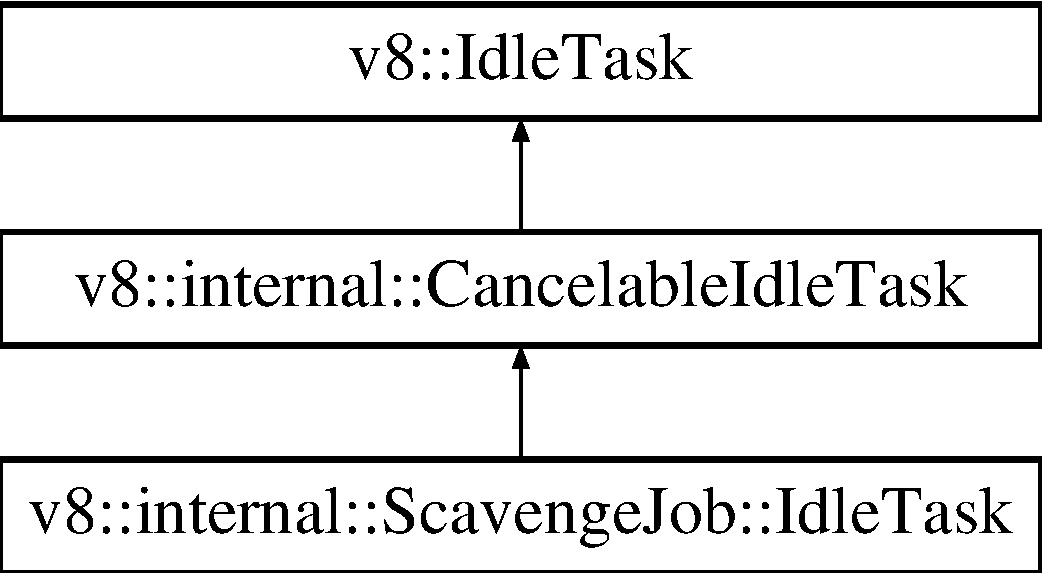
\includegraphics[height=3.000000cm]{classv8_1_1IdleTask}
\end{center}
\end{figure}
\subsection*{Public Member Functions}
\begin{DoxyCompactItemize}
\item 
\mbox{\Hypertarget{classv8_1_1IdleTask_a4f2f238f551b3b2212adffcd5ee2f314}\label{classv8_1_1IdleTask_a4f2f238f551b3b2212adffcd5ee2f314}} 
virtual void {\bfseries Run} (double deadline\+\_\+in\+\_\+seconds)=0
\end{DoxyCompactItemize}


\subsection{Detailed Description}
An \mbox{\hyperlink{classv8_1_1IdleTask}{Idle\+Task}} represents a unit of work to be performed in idle time. The Run method is invoked with an argument that specifies the deadline in seconds returned by Monotonically\+Increasing\+Time(). The idle task is expected to complete by this deadline. 

Definition at line 36 of file v8-\/platform.\+h.



The documentation for this class was generated from the following file\+:\begin{DoxyCompactItemize}
\item 
v8/include/v8-\/platform.\+h\end{DoxyCompactItemize}

\hypertarget{structv8_1_1IndexedPropertyHandlerConfiguration}{}\section{v8\+:\+:Indexed\+Property\+Handler\+Configuration Struct Reference}
\label{structv8_1_1IndexedPropertyHandlerConfiguration}\index{v8\+::\+Indexed\+Property\+Handler\+Configuration@{v8\+::\+Indexed\+Property\+Handler\+Configuration}}
\subsection*{Public Member Functions}
\begin{DoxyCompactItemize}
\item 
\mbox{\Hypertarget{structv8_1_1IndexedPropertyHandlerConfiguration_a4c66c201ea6884e34c7ff2605eef5403}\label{structv8_1_1IndexedPropertyHandlerConfiguration_a4c66c201ea6884e34c7ff2605eef5403}} 
{\bfseries Indexed\+Property\+Handler\+Configuration} (\mbox{\hyperlink{namespacev8_a48e7816ba64447bf32a25d194588daaf}{Indexed\+Property\+Getter\+Callback}} getter, \mbox{\hyperlink{namespacev8_a4ac7cc6185ebc8b6a199f9fa8e6bf5c3}{Indexed\+Property\+Setter\+Callback}} setter, \mbox{\hyperlink{namespacev8_a980b62c33eb664783e61e25c3b27f9ee}{Indexed\+Property\+Query\+Callback}} query, \mbox{\hyperlink{namespacev8_a53863728de14cde48dd6543207b2f2da}{Indexed\+Property\+Deleter\+Callback}} deleter, \mbox{\hyperlink{namespacev8_adbb0a6d5537371953f9ba807d4f6275e}{Indexed\+Property\+Enumerator\+Callback}} enumerator, \mbox{\hyperlink{namespacev8_a967435db933fa9798caac467948499df}{Indexed\+Property\+Definer\+Callback}} definer, \mbox{\hyperlink{namespacev8_a7506e91d70d885b5cbeabdf870ac0e88}{Indexed\+Property\+Descriptor\+Callback}} descriptor, \mbox{\hyperlink{classv8_1_1Local}{Local}}$<$ \mbox{\hyperlink{classv8_1_1Value}{Value}} $>$ data=\mbox{\hyperlink{classv8_1_1Local}{Local}}$<$ \mbox{\hyperlink{classv8_1_1Value}{Value}} $>$(), \mbox{\hyperlink{namespacev8_af4789f0aeb8680e353901a35810cac1a}{Property\+Handler\+Flags}} flags=\mbox{\hyperlink{namespacev8_af4789f0aeb8680e353901a35810cac1aa35c3ace1970663a16e5c65baa5941b13}{Property\+Handler\+Flags\+::k\+None}})
\item 
\mbox{\hyperlink{structv8_1_1IndexedPropertyHandlerConfiguration_a2fb34a4a34c19fce4654c1e02151164b}{Indexed\+Property\+Handler\+Configuration}} (\mbox{\hyperlink{namespacev8_a48e7816ba64447bf32a25d194588daaf}{Indexed\+Property\+Getter\+Callback}} getter=nullptr, \mbox{\hyperlink{namespacev8_a4ac7cc6185ebc8b6a199f9fa8e6bf5c3}{Indexed\+Property\+Setter\+Callback}} setter=nullptr, \mbox{\hyperlink{namespacev8_a980b62c33eb664783e61e25c3b27f9ee}{Indexed\+Property\+Query\+Callback}} query=nullptr, \mbox{\hyperlink{namespacev8_a53863728de14cde48dd6543207b2f2da}{Indexed\+Property\+Deleter\+Callback}} deleter=nullptr, \mbox{\hyperlink{namespacev8_adbb0a6d5537371953f9ba807d4f6275e}{Indexed\+Property\+Enumerator\+Callback}} enumerator=nullptr, \mbox{\hyperlink{classv8_1_1Local}{Local}}$<$ \mbox{\hyperlink{classv8_1_1Value}{Value}} $>$ data=\mbox{\hyperlink{classv8_1_1Local}{Local}}$<$ \mbox{\hyperlink{classv8_1_1Value}{Value}} $>$(), \mbox{\hyperlink{namespacev8_af4789f0aeb8680e353901a35810cac1a}{Property\+Handler\+Flags}} flags=\mbox{\hyperlink{namespacev8_af4789f0aeb8680e353901a35810cac1aa35c3ace1970663a16e5c65baa5941b13}{Property\+Handler\+Flags\+::k\+None}})
\item 
\mbox{\Hypertarget{structv8_1_1IndexedPropertyHandlerConfiguration_a52a8b33b496a43f6864d6073f4951baf}\label{structv8_1_1IndexedPropertyHandlerConfiguration_a52a8b33b496a43f6864d6073f4951baf}} 
{\bfseries Indexed\+Property\+Handler\+Configuration} (\mbox{\hyperlink{namespacev8_a48e7816ba64447bf32a25d194588daaf}{Indexed\+Property\+Getter\+Callback}} getter, \mbox{\hyperlink{namespacev8_a4ac7cc6185ebc8b6a199f9fa8e6bf5c3}{Indexed\+Property\+Setter\+Callback}} setter, \mbox{\hyperlink{namespacev8_a7506e91d70d885b5cbeabdf870ac0e88}{Indexed\+Property\+Descriptor\+Callback}} descriptor, \mbox{\hyperlink{namespacev8_a53863728de14cde48dd6543207b2f2da}{Indexed\+Property\+Deleter\+Callback}} deleter, \mbox{\hyperlink{namespacev8_adbb0a6d5537371953f9ba807d4f6275e}{Indexed\+Property\+Enumerator\+Callback}} enumerator, \mbox{\hyperlink{namespacev8_a967435db933fa9798caac467948499df}{Indexed\+Property\+Definer\+Callback}} definer, \mbox{\hyperlink{classv8_1_1Local}{Local}}$<$ \mbox{\hyperlink{classv8_1_1Value}{Value}} $>$ data=\mbox{\hyperlink{classv8_1_1Local}{Local}}$<$ \mbox{\hyperlink{classv8_1_1Value}{Value}} $>$(), \mbox{\hyperlink{namespacev8_af4789f0aeb8680e353901a35810cac1a}{Property\+Handler\+Flags}} flags=\mbox{\hyperlink{namespacev8_af4789f0aeb8680e353901a35810cac1aa35c3ace1970663a16e5c65baa5941b13}{Property\+Handler\+Flags\+::k\+None}})
\end{DoxyCompactItemize}
\subsection*{Data Fields}
\begin{DoxyCompactItemize}
\item 
\mbox{\Hypertarget{structv8_1_1IndexedPropertyHandlerConfiguration_a026928df0639b471a63c8795f0d13190}\label{structv8_1_1IndexedPropertyHandlerConfiguration_a026928df0639b471a63c8795f0d13190}} 
\mbox{\hyperlink{namespacev8_a48e7816ba64447bf32a25d194588daaf}{Indexed\+Property\+Getter\+Callback}} {\bfseries getter}
\item 
\mbox{\Hypertarget{structv8_1_1IndexedPropertyHandlerConfiguration_a4c199d5b9d842a9bc420118b7d3e4f5a}\label{structv8_1_1IndexedPropertyHandlerConfiguration_a4c199d5b9d842a9bc420118b7d3e4f5a}} 
\mbox{\hyperlink{namespacev8_a4ac7cc6185ebc8b6a199f9fa8e6bf5c3}{Indexed\+Property\+Setter\+Callback}} {\bfseries setter}
\item 
\mbox{\Hypertarget{structv8_1_1IndexedPropertyHandlerConfiguration_ab38e189fc5bc94928e3b8489c5004a2e}\label{structv8_1_1IndexedPropertyHandlerConfiguration_ab38e189fc5bc94928e3b8489c5004a2e}} 
\mbox{\hyperlink{namespacev8_a980b62c33eb664783e61e25c3b27f9ee}{Indexed\+Property\+Query\+Callback}} {\bfseries query}
\item 
\mbox{\Hypertarget{structv8_1_1IndexedPropertyHandlerConfiguration_acc45ef8977b42a9655df080acbd6acbe}\label{structv8_1_1IndexedPropertyHandlerConfiguration_acc45ef8977b42a9655df080acbd6acbe}} 
\mbox{\hyperlink{namespacev8_a53863728de14cde48dd6543207b2f2da}{Indexed\+Property\+Deleter\+Callback}} {\bfseries deleter}
\item 
\mbox{\Hypertarget{structv8_1_1IndexedPropertyHandlerConfiguration_aaa1cc6503b7fc76ac989f294e3af3ddb}\label{structv8_1_1IndexedPropertyHandlerConfiguration_aaa1cc6503b7fc76ac989f294e3af3ddb}} 
\mbox{\hyperlink{namespacev8_adbb0a6d5537371953f9ba807d4f6275e}{Indexed\+Property\+Enumerator\+Callback}} {\bfseries enumerator}
\item 
\mbox{\Hypertarget{structv8_1_1IndexedPropertyHandlerConfiguration_a3f0dd03984595c2676eaf6a8267fb5e5}\label{structv8_1_1IndexedPropertyHandlerConfiguration_a3f0dd03984595c2676eaf6a8267fb5e5}} 
\mbox{\hyperlink{namespacev8_a967435db933fa9798caac467948499df}{Indexed\+Property\+Definer\+Callback}} {\bfseries definer}
\item 
\mbox{\Hypertarget{structv8_1_1IndexedPropertyHandlerConfiguration_a4b611dc26cc11391ba430b84f87b53c5}\label{structv8_1_1IndexedPropertyHandlerConfiguration_a4b611dc26cc11391ba430b84f87b53c5}} 
\mbox{\hyperlink{namespacev8_a7506e91d70d885b5cbeabdf870ac0e88}{Indexed\+Property\+Descriptor\+Callback}} {\bfseries descriptor}
\item 
\mbox{\Hypertarget{structv8_1_1IndexedPropertyHandlerConfiguration_abbedfb5f55042decce382b4482bd5bbc}\label{structv8_1_1IndexedPropertyHandlerConfiguration_abbedfb5f55042decce382b4482bd5bbc}} 
\mbox{\hyperlink{classv8_1_1Local}{Local}}$<$ \mbox{\hyperlink{classv8_1_1Value}{Value}} $>$ {\bfseries data}
\item 
\mbox{\Hypertarget{structv8_1_1IndexedPropertyHandlerConfiguration_a435b9a3495ba031611bd7feea4cb981b}\label{structv8_1_1IndexedPropertyHandlerConfiguration_a435b9a3495ba031611bd7feea4cb981b}} 
\mbox{\hyperlink{namespacev8_af4789f0aeb8680e353901a35810cac1a}{Property\+Handler\+Flags}} {\bfseries flags}
\end{DoxyCompactItemize}


\subsection{Constructor \& Destructor Documentation}
\mbox{\Hypertarget{structv8_1_1IndexedPropertyHandlerConfiguration_a2fb34a4a34c19fce4654c1e02151164b}\label{structv8_1_1IndexedPropertyHandlerConfiguration_a2fb34a4a34c19fce4654c1e02151164b}} 
\index{v8\+::\+Indexed\+Property\+Handler\+Configuration@{v8\+::\+Indexed\+Property\+Handler\+Configuration}!Indexed\+Property\+Handler\+Configuration@{Indexed\+Property\+Handler\+Configuration}}
\index{Indexed\+Property\+Handler\+Configuration@{Indexed\+Property\+Handler\+Configuration}!v8\+::\+Indexed\+Property\+Handler\+Configuration@{v8\+::\+Indexed\+Property\+Handler\+Configuration}}
\subsubsection{\texorpdfstring{Indexed\+Property\+Handler\+Configuration()}{IndexedPropertyHandlerConfiguration()}}
{\footnotesize\ttfamily v8\+::\+Indexed\+Property\+Handler\+Configuration\+::\+Indexed\+Property\+Handler\+Configuration (\begin{DoxyParamCaption}\item[{\mbox{\hyperlink{namespacev8_a48e7816ba64447bf32a25d194588daaf}{Indexed\+Property\+Getter\+Callback}}}]{getter = {\ttfamily nullptr},  }\item[{\mbox{\hyperlink{namespacev8_a4ac7cc6185ebc8b6a199f9fa8e6bf5c3}{Indexed\+Property\+Setter\+Callback}}}]{setter = {\ttfamily nullptr},  }\item[{\mbox{\hyperlink{namespacev8_a980b62c33eb664783e61e25c3b27f9ee}{Indexed\+Property\+Query\+Callback}}}]{query = {\ttfamily nullptr},  }\item[{\mbox{\hyperlink{namespacev8_a53863728de14cde48dd6543207b2f2da}{Indexed\+Property\+Deleter\+Callback}}}]{deleter = {\ttfamily nullptr},  }\item[{\mbox{\hyperlink{namespacev8_adbb0a6d5537371953f9ba807d4f6275e}{Indexed\+Property\+Enumerator\+Callback}}}]{enumerator = {\ttfamily nullptr},  }\item[{\mbox{\hyperlink{classv8_1_1Local}{Local}}$<$ \mbox{\hyperlink{classv8_1_1Value}{Value}} $>$}]{data = {\ttfamily \mbox{\hyperlink{classv8_1_1Local}{Local}}$<$\mbox{\hyperlink{classv8_1_1Value}{Value}}$>$()},  }\item[{\mbox{\hyperlink{namespacev8_af4789f0aeb8680e353901a35810cac1a}{Property\+Handler\+Flags}}}]{flags = {\ttfamily \mbox{\hyperlink{namespacev8_af4789f0aeb8680e353901a35810cac1aa35c3ace1970663a16e5c65baa5941b13}{Property\+Handler\+Flags\+::k\+None}}} }\end{DoxyParamCaption})\hspace{0.3cm}{\ttfamily [inline]}}


\begin{DoxyParams}{Parameters}
{\em getter} & Note\+: getter is required \\
\hline
\end{DoxyParams}


The documentation for this struct was generated from the following file\+:\begin{DoxyCompactItemize}
\item 
v8/include/v8.\+h\end{DoxyCompactItemize}

\hypertarget{classv8_1_1Int16Array}{\section{v8\-:\-:Int16\-Array Class Reference}
\label{classv8_1_1Int16Array}\index{v8\-::\-Int16\-Array@{v8\-::\-Int16\-Array}}
}


{\ttfamily \#include $<$v8.\-h$>$}

Inheritance diagram for v8\-:\-:Int16\-Array\-:\begin{figure}[H]
\begin{center}
\leavevmode
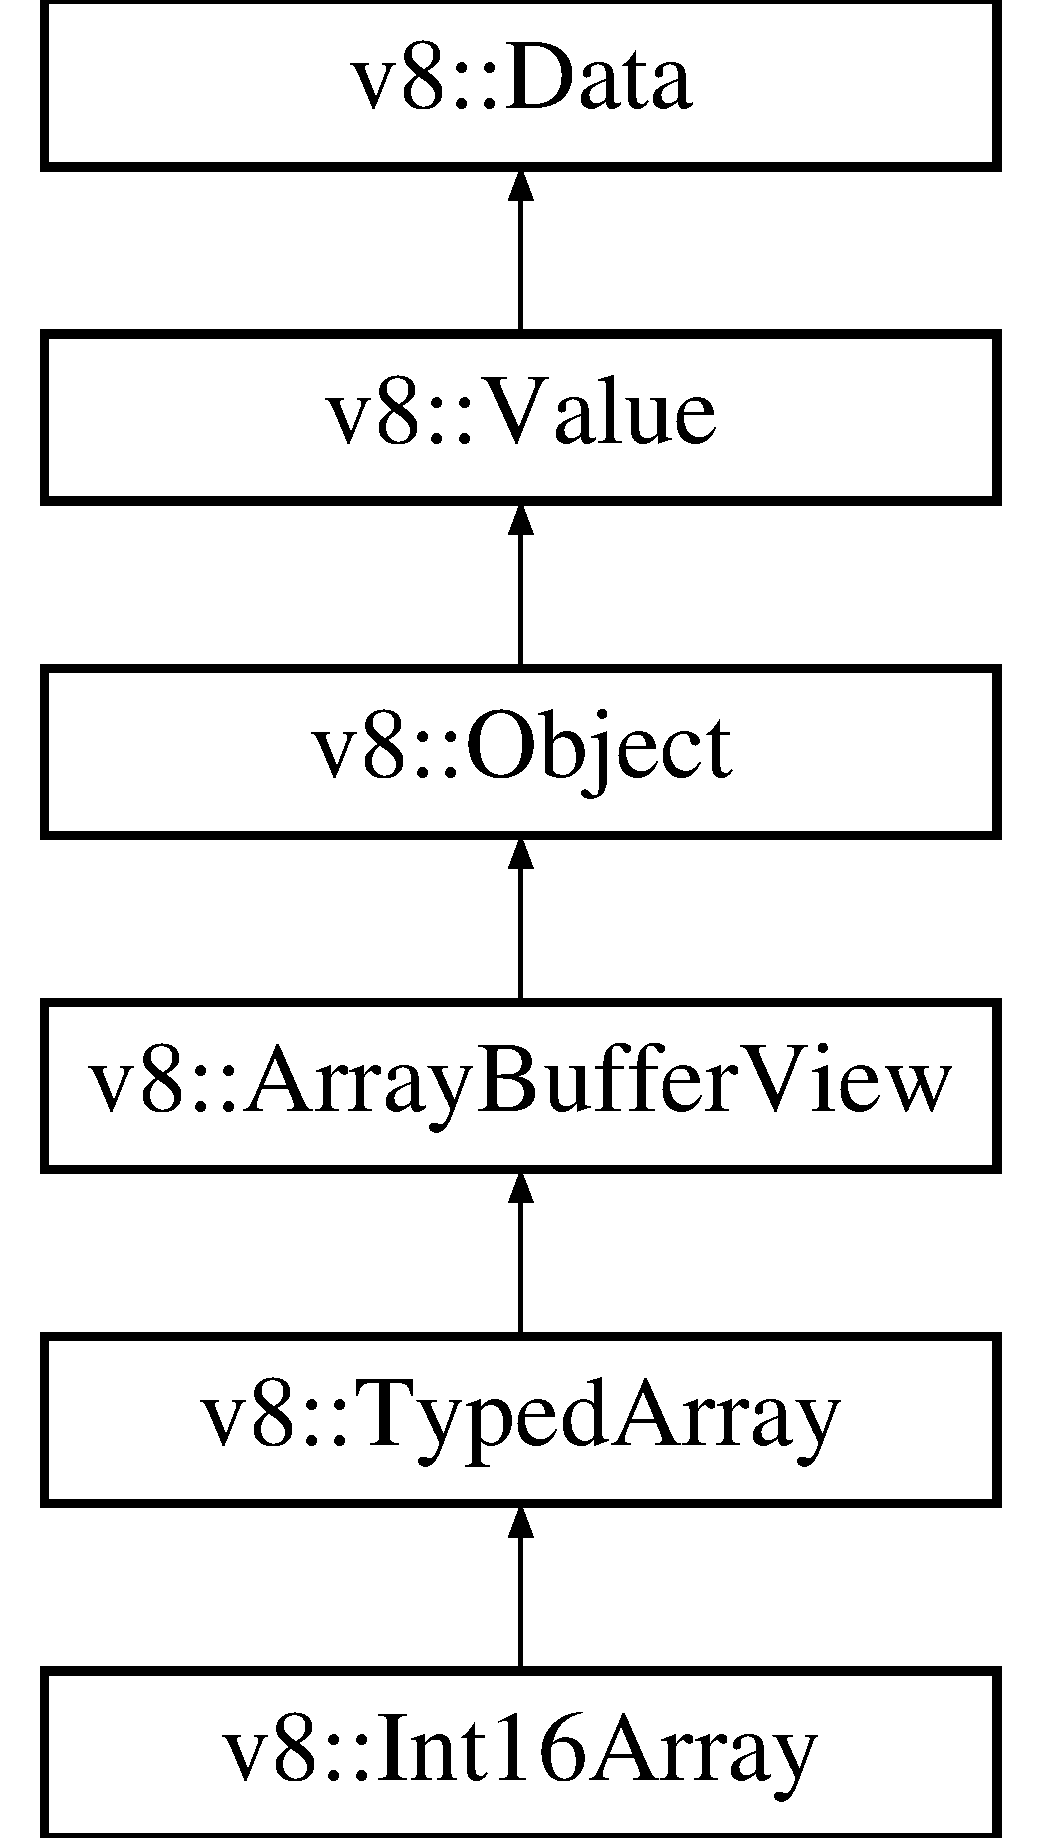
\includegraphics[height=6.000000cm]{classv8_1_1Int16Array}
\end{center}
\end{figure}
\subsection*{Static Public Member Functions}
\begin{DoxyCompactItemize}
\item 
\hypertarget{classv8_1_1Int16Array_adc49fddf7e0b2c719085f5f9af3762e5}{static \hyperlink{classv8_1_1Local}{Local}$<$ \hyperlink{classv8_1_1Int16Array}{Int16\-Array} $>$ {\bfseries New} (\hyperlink{classv8_1_1Handle}{Handle}$<$ \hyperlink{classv8_1_1ArrayBuffer}{Array\-Buffer} $>$ array\-\_\-buffer, size\-\_\-t byte\-\_\-offset, size\-\_\-t length)}\label{classv8_1_1Int16Array_adc49fddf7e0b2c719085f5f9af3762e5}

\item 
\hypertarget{classv8_1_1Int16Array_abef12f11ace9c74a4ce451db28b954e5}{static V8\-\_\-\-I\-N\-L\-I\-N\-E \hyperlink{classv8_1_1Int16Array}{Int16\-Array} $\ast$ {\bfseries Cast} (\hyperlink{classv8_1_1Value}{Value} $\ast$obj)}\label{classv8_1_1Int16Array_abef12f11ace9c74a4ce451db28b954e5}

\end{DoxyCompactItemize}
\subsection*{Additional Inherited Members}


\subsection{Detailed Description}
An instance of \hyperlink{classv8_1_1Int16Array}{Int16\-Array} constructor (E\-S6 draft 15.\-13.\-6). This A\-P\-I is experimental and may change significantly. 

The documentation for this class was generated from the following file\-:\begin{DoxyCompactItemize}
\item 
v8/include/v8.\-h\end{DoxyCompactItemize}

\hypertarget{classv8_1_1Int32}{}\section{v8\+:\+:Int32 Class Reference}
\label{classv8_1_1Int32}\index{v8\+::\+Int32@{v8\+::\+Int32}}


{\ttfamily \#include $<$v8.\+h$>$}

Inheritance diagram for v8\+:\+:Int32\+:\begin{figure}[H]
\begin{center}
\leavevmode
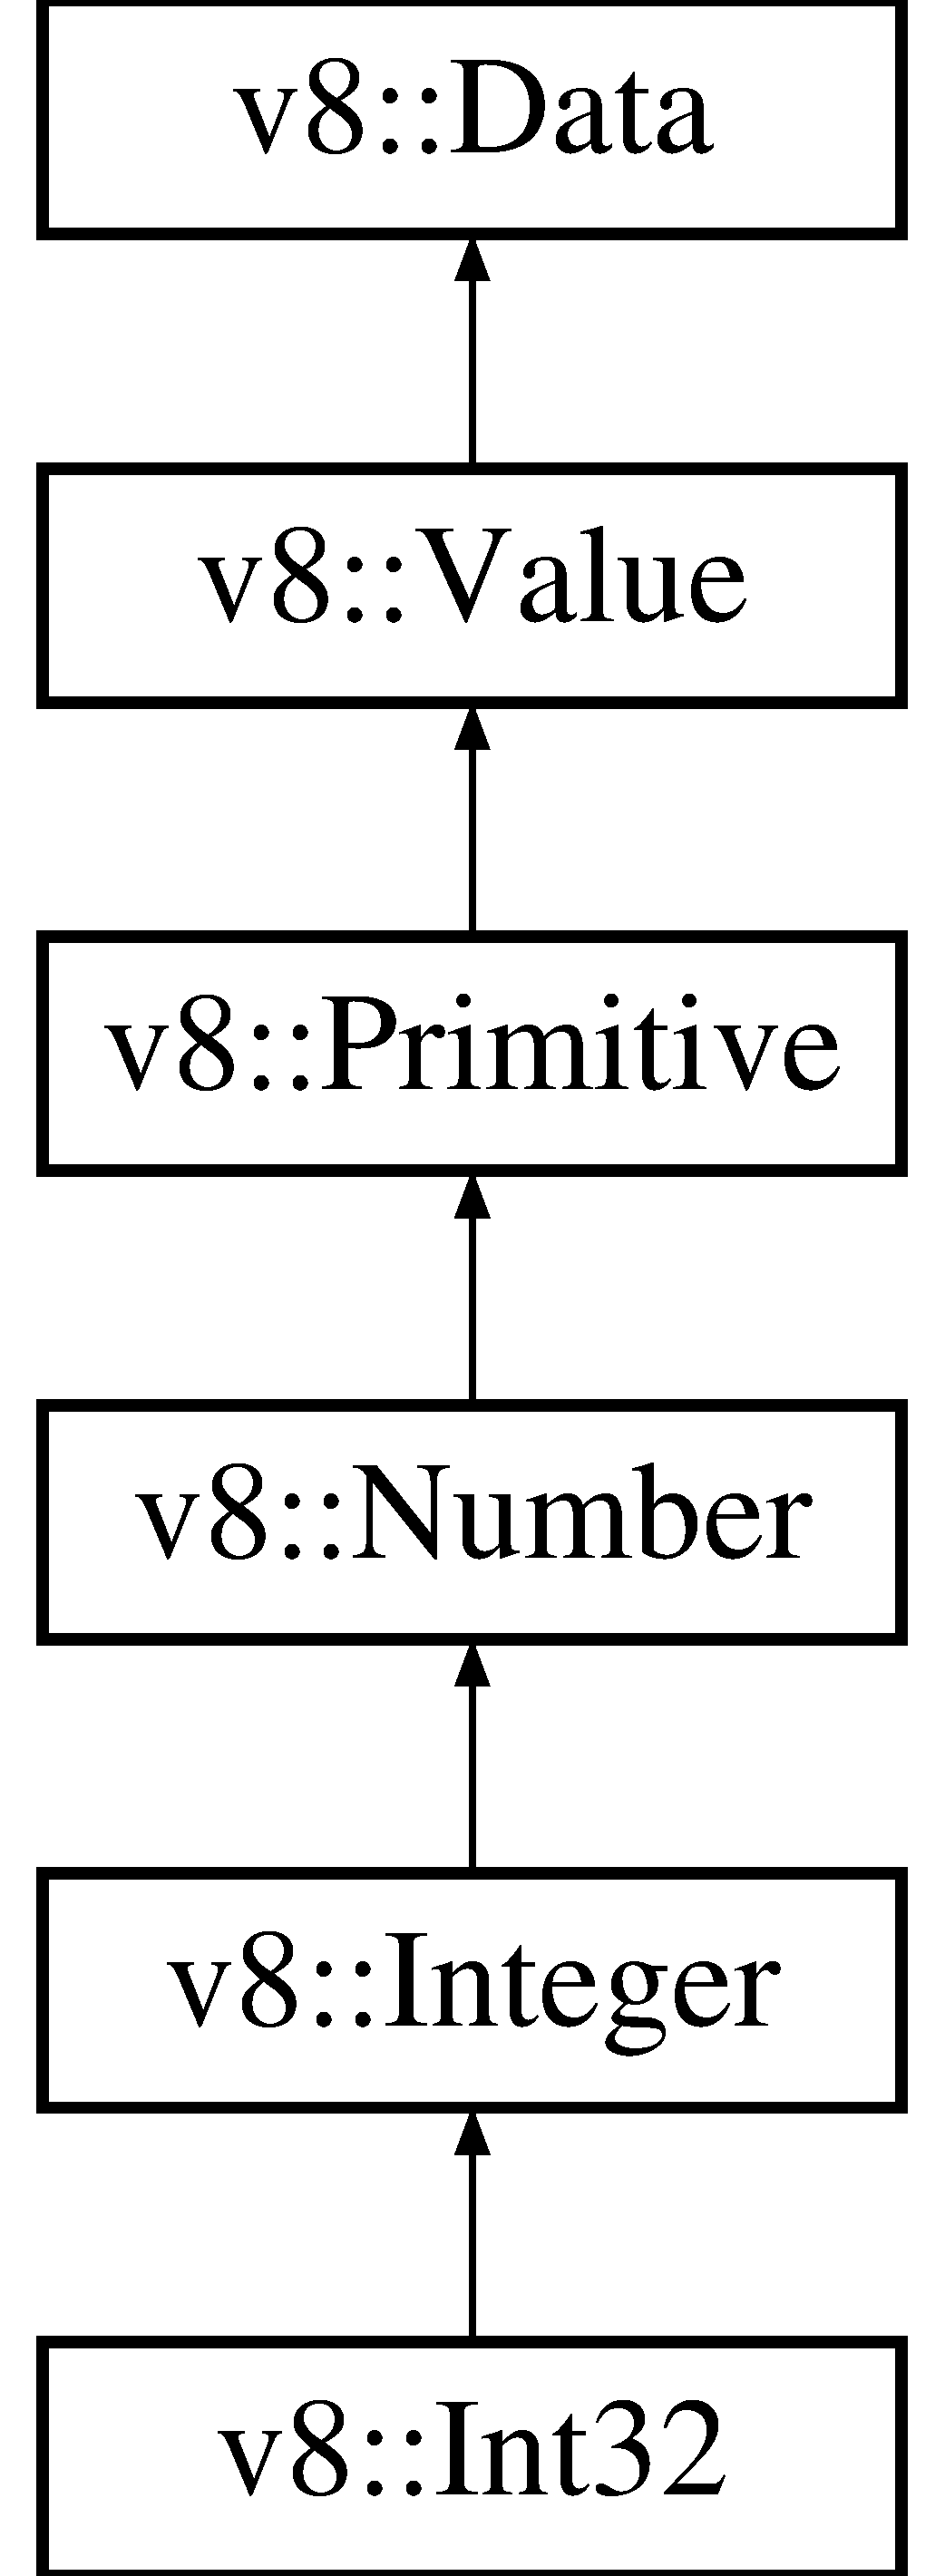
\includegraphics[height=6.000000cm]{classv8_1_1Int32}
\end{center}
\end{figure}
\subsection*{Public Member Functions}
\begin{DoxyCompactItemize}
\item 
int32\+\_\+t {\bfseries Value} () const \hypertarget{classv8_1_1Int32_a74860c6a524e1fb3f7b685ab0896be4b}{}\label{classv8_1_1Int32_a74860c6a524e1fb3f7b685ab0896be4b}

\end{DoxyCompactItemize}
\subsection*{Static Public Member Functions}
\begin{DoxyCompactItemize}
\item 
static V8\+\_\+\+I\+N\+L\+I\+NE \hyperlink{classv8_1_1Int32}{Int32} $\ast$ {\bfseries Cast} (\hyperlink{classv8_1_1Value}{v8\+::\+Value} $\ast$obj)\hypertarget{classv8_1_1Int32_a910c59c30a7f5f3c96afd0ba10d5339b}{}\label{classv8_1_1Int32_a910c59c30a7f5f3c96afd0ba10d5339b}

\end{DoxyCompactItemize}


\subsection{Detailed Description}
A Java\+Script value representing a 32-\/bit signed integer. 

The documentation for this class was generated from the following file\+:\begin{DoxyCompactItemize}
\item 
v8/include/v8.\+h\end{DoxyCompactItemize}

\hypertarget{classv8_1_1Int32Array}{}\section{v8\+:\+:Int32\+Array Class Reference}
\label{classv8_1_1Int32Array}\index{v8\+::\+Int32\+Array@{v8\+::\+Int32\+Array}}


{\ttfamily \#include $<$v8.\+h$>$}

Inheritance diagram for v8\+:\+:Int32\+Array\+:\begin{figure}[H]
\begin{center}
\leavevmode
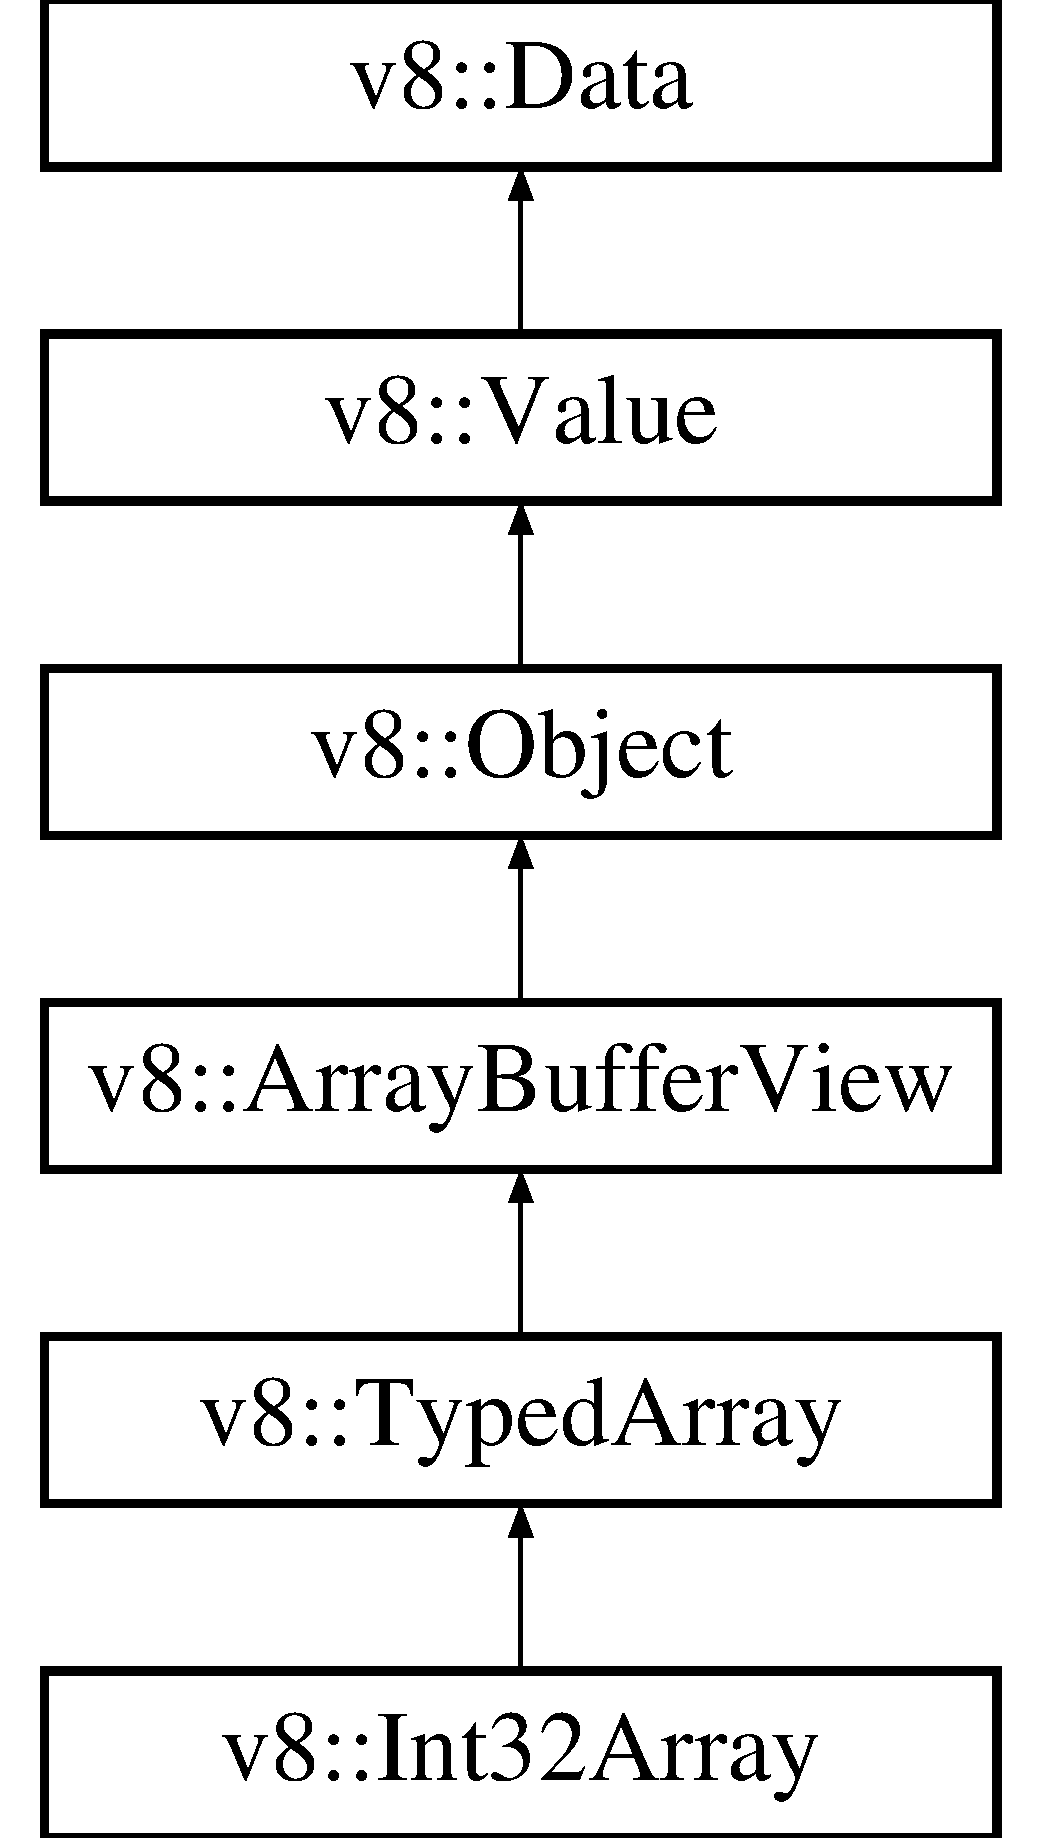
\includegraphics[height=6.000000cm]{classv8_1_1Int32Array}
\end{center}
\end{figure}
\subsection*{Static Public Member Functions}
\begin{DoxyCompactItemize}
\item 
\hypertarget{classv8_1_1Int32Array_a03adbd44725e3325d10bcc448e8bfd75}{}static \hyperlink{classv8_1_1Local}{Local}$<$ \hyperlink{classv8_1_1Int32Array}{Int32\+Array} $>$ {\bfseries New} (\hyperlink{classv8_1_1Local}{Local}$<$ \hyperlink{classv8_1_1ArrayBuffer}{Array\+Buffer} $>$ array\+\_\+buffer, size\+\_\+t byte\+\_\+offset, size\+\_\+t length)\label{classv8_1_1Int32Array_a03adbd44725e3325d10bcc448e8bfd75}

\item 
\hypertarget{classv8_1_1Int32Array_acf112fc9df4e0bf2791be73264779905}{}static \hyperlink{classv8_1_1Local}{Local}$<$ \hyperlink{classv8_1_1Int32Array}{Int32\+Array} $>$ {\bfseries New} (\hyperlink{classv8_1_1Local}{Local}$<$ \hyperlink{classv8_1_1SharedArrayBuffer}{Shared\+Array\+Buffer} $>$ shared\+\_\+array\+\_\+buffer, size\+\_\+t byte\+\_\+offset, size\+\_\+t length)\label{classv8_1_1Int32Array_acf112fc9df4e0bf2791be73264779905}

\item 
\hypertarget{classv8_1_1Int32Array_afe7cdf534deadc3d872d8a43778809f1}{}static V8\+\_\+\+I\+N\+L\+I\+N\+E \hyperlink{classv8_1_1Int32Array}{Int32\+Array} $\ast$ {\bfseries Cast} (\hyperlink{classv8_1_1Value}{Value} $\ast$obj)\label{classv8_1_1Int32Array_afe7cdf534deadc3d872d8a43778809f1}

\end{DoxyCompactItemize}
\subsection*{Additional Inherited Members}


\subsection{Detailed Description}
An instance of \hyperlink{classv8_1_1Int32Array}{Int32\+Array} constructor (E\+S6 draft 15.\+13.\+6). This A\+P\+I is experimental and may change significantly. 

The documentation for this class was generated from the following file\+:\begin{DoxyCompactItemize}
\item 
v8/include/v8.\+h\end{DoxyCompactItemize}

\hypertarget{classv8_1_1Int8Array}{}\section{v8\+:\+:Int8\+Array Class Reference}
\label{classv8_1_1Int8Array}\index{v8\+::\+Int8\+Array@{v8\+::\+Int8\+Array}}


{\ttfamily \#include $<$v8.\+h$>$}

Inheritance diagram for v8\+:\+:Int8\+Array\+:\begin{figure}[H]
\begin{center}
\leavevmode
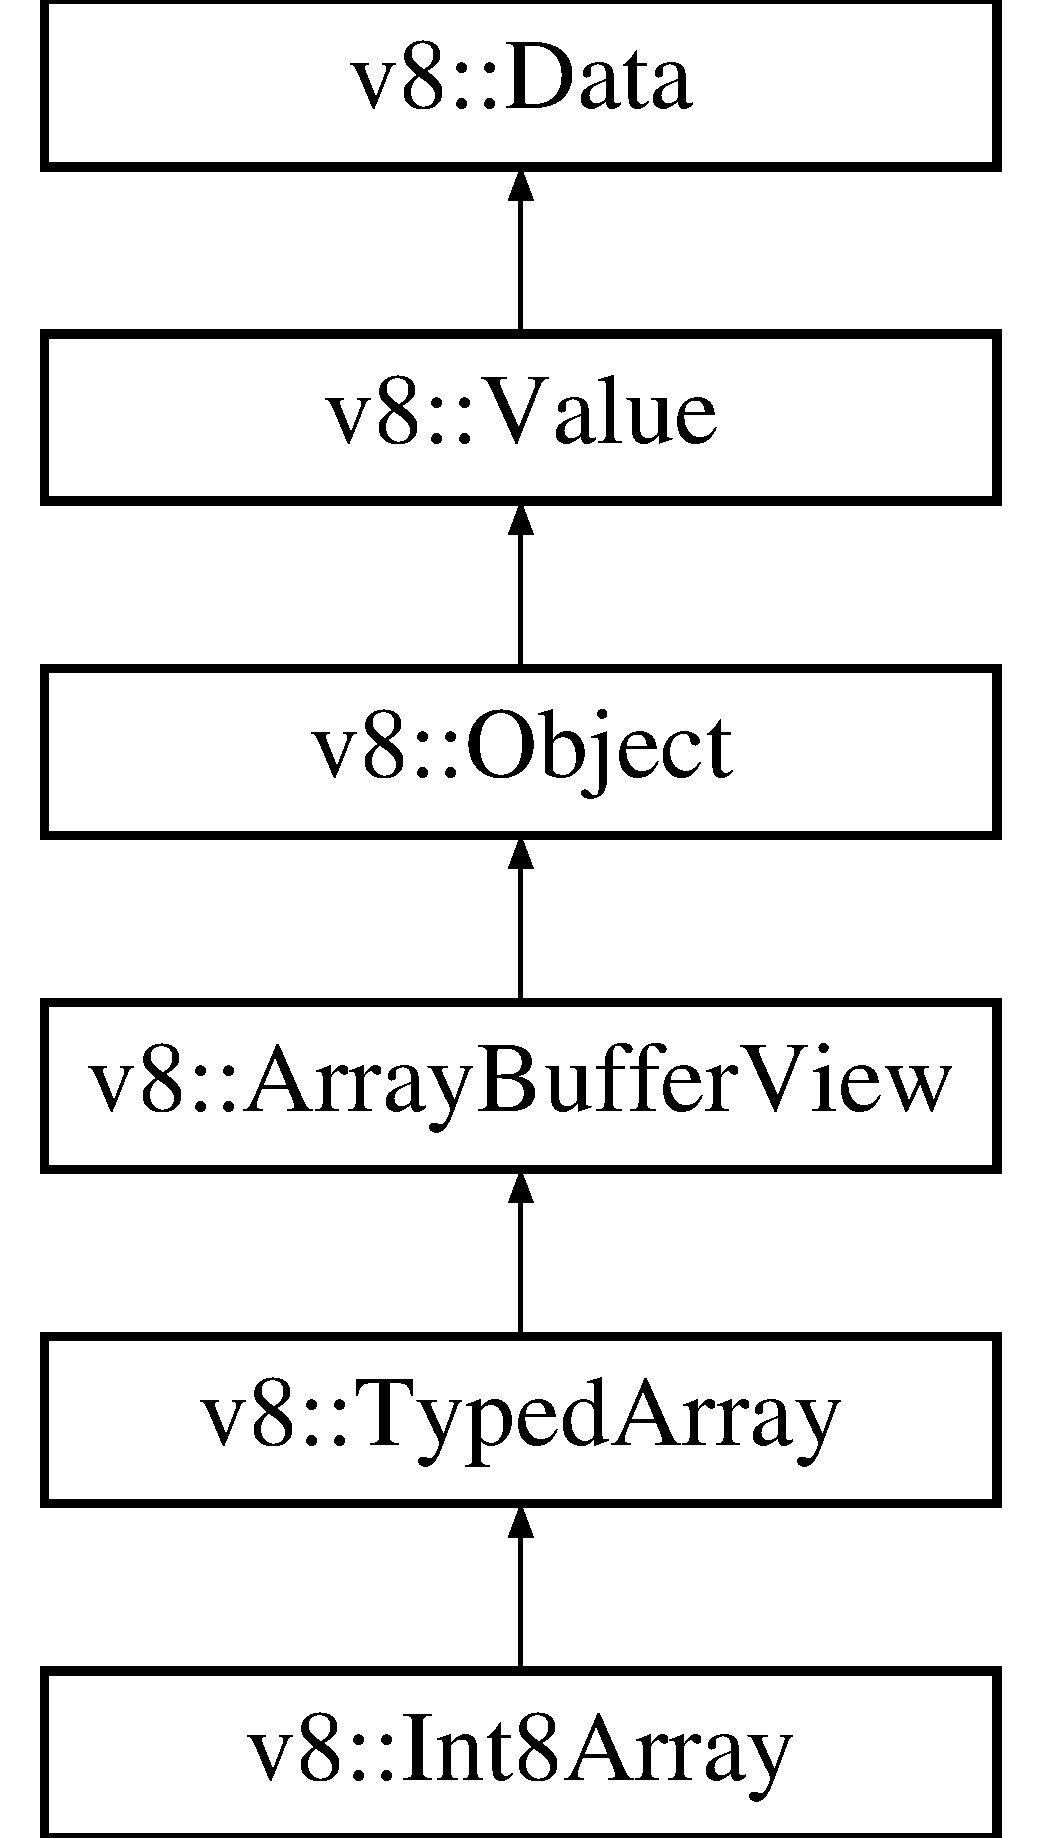
\includegraphics[height=6.000000cm]{classv8_1_1Int8Array}
\end{center}
\end{figure}
\subsection*{Static Public Member Functions}
\begin{DoxyCompactItemize}
\item 
\mbox{\Hypertarget{classv8_1_1Int8Array_a13e12d1a556aa2ef92271484a10acd21}\label{classv8_1_1Int8Array_a13e12d1a556aa2ef92271484a10acd21}} 
static \mbox{\hyperlink{classv8_1_1Local}{Local}}$<$ \mbox{\hyperlink{classv8_1_1Int8Array}{Int8\+Array}} $>$ {\bfseries New} (\mbox{\hyperlink{classv8_1_1Local}{Local}}$<$ \mbox{\hyperlink{classv8_1_1ArrayBuffer}{Array\+Buffer}} $>$ array\+\_\+buffer, \mbox{\hyperlink{classsize__t}{size\+\_\+t}} byte\+\_\+offset, \mbox{\hyperlink{classsize__t}{size\+\_\+t}} length)
\item 
\mbox{\Hypertarget{classv8_1_1Int8Array_a364d52f1dc634e637321b2a9f9ec4dd8}\label{classv8_1_1Int8Array_a364d52f1dc634e637321b2a9f9ec4dd8}} 
static \mbox{\hyperlink{classv8_1_1Local}{Local}}$<$ \mbox{\hyperlink{classv8_1_1Int8Array}{Int8\+Array}} $>$ {\bfseries New} (\mbox{\hyperlink{classv8_1_1Local}{Local}}$<$ \mbox{\hyperlink{classv8_1_1SharedArrayBuffer}{Shared\+Array\+Buffer}} $>$ shared\+\_\+array\+\_\+buffer, \mbox{\hyperlink{classsize__t}{size\+\_\+t}} byte\+\_\+offset, \mbox{\hyperlink{classsize__t}{size\+\_\+t}} length)
\item 
\mbox{\Hypertarget{classv8_1_1Int8Array_a201a6b46e2cc455830d62c57bc8b4a3e}\label{classv8_1_1Int8Array_a201a6b46e2cc455830d62c57bc8b4a3e}} 
static V8\+\_\+\+I\+N\+L\+I\+NE \mbox{\hyperlink{classv8_1_1Int8Array}{Int8\+Array}} $\ast$ {\bfseries Cast} (\mbox{\hyperlink{classv8_1_1Value}{Value}} $\ast$obj)
\end{DoxyCompactItemize}
\subsection*{Additional Inherited Members}


\subsection{Detailed Description}
An instance of \mbox{\hyperlink{classv8_1_1Int8Array}{Int8\+Array}} constructor (E\+S6 draft 15.\+13.\+6). 

Definition at line 4797 of file v8.\+h.



The documentation for this class was generated from the following file\+:\begin{DoxyCompactItemize}
\item 
v8/include/v8.\+h\end{DoxyCompactItemize}

\hypertarget{classv8_1_1Integer}{}\section{v8\+:\+:Integer Class Reference}
\label{classv8_1_1Integer}\index{v8\+::\+Integer@{v8\+::\+Integer}}


{\ttfamily \#include $<$v8.\+h$>$}

Inheritance diagram for v8\+:\+:Integer\+:\begin{figure}[H]
\begin{center}
\leavevmode
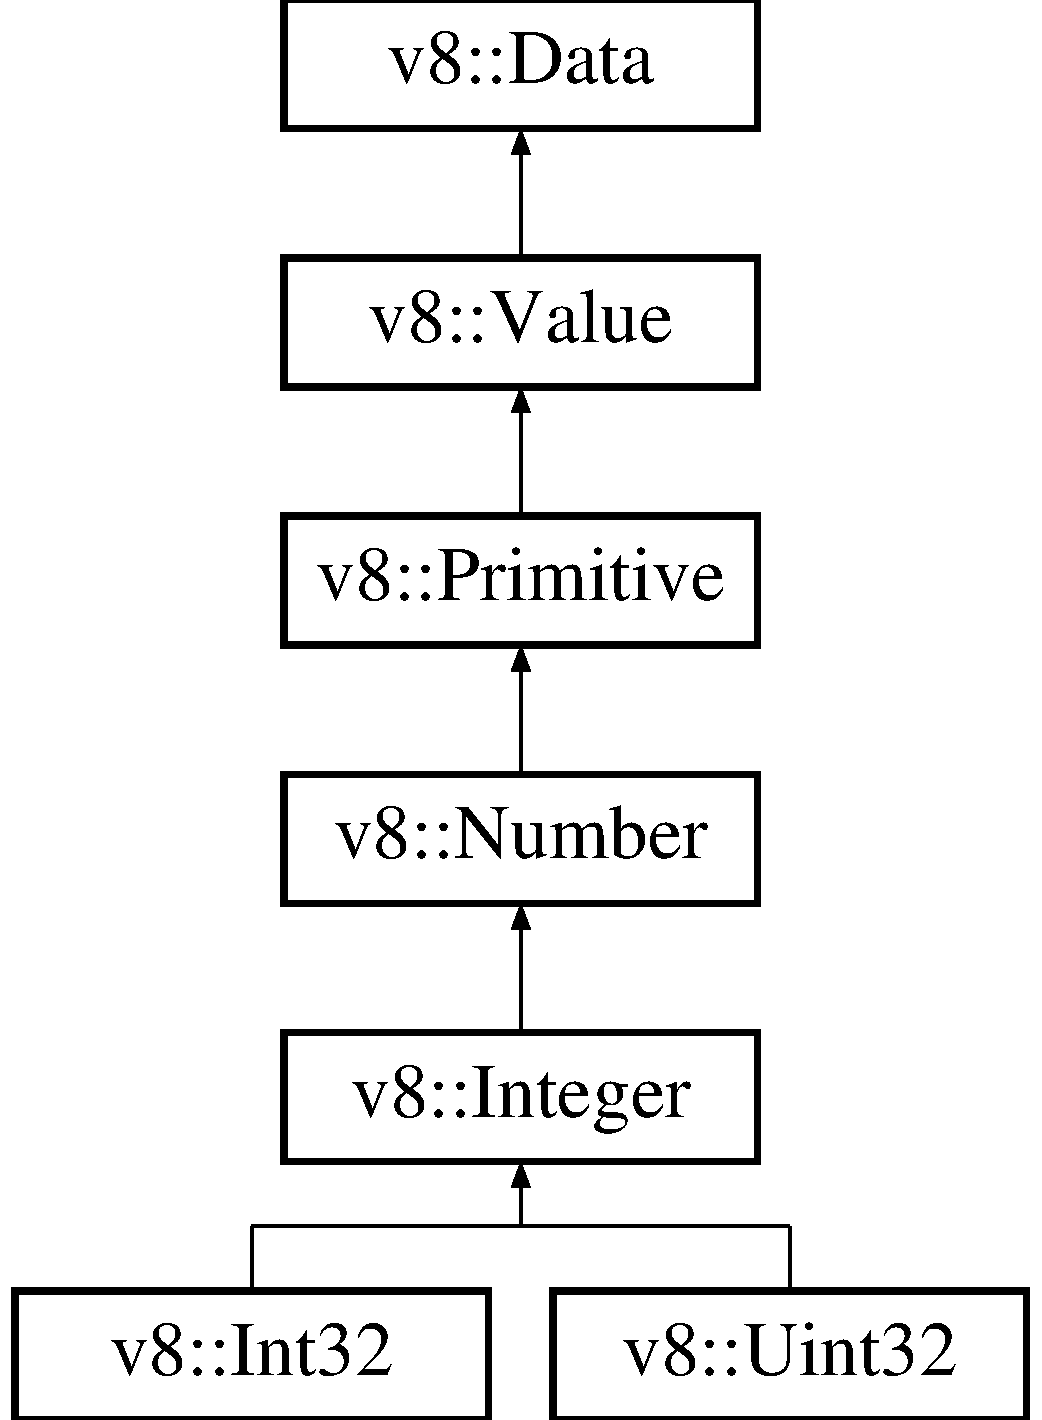
\includegraphics[height=6.000000cm]{classv8_1_1Integer}
\end{center}
\end{figure}
\subsection*{Public Member Functions}
\begin{DoxyCompactItemize}
\item 
int64\+\_\+t {\bfseries Value} () const \hypertarget{classv8_1_1Integer_a93bcfb39090631a3ff95843463183c9c}{}\label{classv8_1_1Integer_a93bcfb39090631a3ff95843463183c9c}

\end{DoxyCompactItemize}
\subsection*{Static Public Member Functions}
\begin{DoxyCompactItemize}
\item 
static \hyperlink{classv8_1_1Local}{Local}$<$ \hyperlink{classv8_1_1Integer}{Integer} $>$ {\bfseries New} (\hyperlink{classv8_1_1Isolate}{Isolate} $\ast$isolate, int32\+\_\+t value)\hypertarget{classv8_1_1Integer_a730d6e093c16d95edb5b92a4d05773d0}{}\label{classv8_1_1Integer_a730d6e093c16d95edb5b92a4d05773d0}

\item 
static \hyperlink{classv8_1_1Local}{Local}$<$ \hyperlink{classv8_1_1Integer}{Integer} $>$ {\bfseries New\+From\+Unsigned} (\hyperlink{classv8_1_1Isolate}{Isolate} $\ast$isolate, uint32\+\_\+t value)\hypertarget{classv8_1_1Integer_a6fbd6e79db802c737cb0bd5a259f134b}{}\label{classv8_1_1Integer_a6fbd6e79db802c737cb0bd5a259f134b}

\item 
static V8\+\_\+\+I\+N\+L\+I\+NE \hyperlink{classv8_1_1Integer}{Integer} $\ast$ {\bfseries Cast} (\hyperlink{classv8_1_1Value}{v8\+::\+Value} $\ast$obj)\hypertarget{classv8_1_1Integer_a886f73d3d8bb91f8235f66d8dccec12a}{}\label{classv8_1_1Integer_a886f73d3d8bb91f8235f66d8dccec12a}

\end{DoxyCompactItemize}


\subsection{Detailed Description}
A Java\+Script value representing a signed integer. 

The documentation for this class was generated from the following file\+:\begin{DoxyCompactItemize}
\item 
v8/include/v8.\+h\end{DoxyCompactItemize}

\hypertarget{classv8_1_1internal_1_1Internals}{}\section{v8\+:\+:internal\+:\+:Internals Class Reference}
\label{classv8_1_1internal_1_1Internals}\index{v8\+::internal\+::\+Internals@{v8\+::internal\+::\+Internals}}


{\ttfamily \#include $<$v8-\/internal.\+h$>$}

\subsection*{Static Public Member Functions}
\begin{DoxyCompactItemize}
\item 
\mbox{\Hypertarget{classv8_1_1internal_1_1Internals_ac5141eba7a786f0fa9f6db658f25d4ba}\label{classv8_1_1internal_1_1Internals_ac5141eba7a786f0fa9f6db658f25d4ba}} 
static V8\+\_\+\+E\+X\+P\+O\+RT void {\bfseries Check\+Initialized\+Impl} (v8\+::\+Isolate $\ast$isolate)
\item 
\mbox{\Hypertarget{classv8_1_1internal_1_1Internals_a1aa4bc86bc011f055fe27d18e0849b8c}\label{classv8_1_1internal_1_1Internals_a1aa4bc86bc011f055fe27d18e0849b8c}} 
static V8\+\_\+\+I\+N\+L\+I\+NE void {\bfseries Check\+Initialized} (v8\+::\+Isolate $\ast$isolate)
\item 
\mbox{\Hypertarget{classv8_1_1internal_1_1Internals_adcdb38643eb538a720dbee4e77acea15}\label{classv8_1_1internal_1_1Internals_adcdb38643eb538a720dbee4e77acea15}} 
static V8\+\_\+\+I\+N\+L\+I\+NE \mbox{\hyperlink{classbool}{bool}} {\bfseries Has\+Heap\+Object\+Tag} (const \mbox{\hyperlink{classuintptr__t}{internal\+::\+Address}} value)
\item 
\mbox{\Hypertarget{classv8_1_1internal_1_1Internals_a7489b2097139fa3f9dca4006178d7c0d}\label{classv8_1_1internal_1_1Internals_a7489b2097139fa3f9dca4006178d7c0d}} 
static V8\+\_\+\+I\+N\+L\+I\+NE \mbox{\hyperlink{classint}{int}} {\bfseries Smi\+Value} (const \mbox{\hyperlink{classuintptr__t}{internal\+::\+Address}} value)
\item 
\mbox{\Hypertarget{classv8_1_1internal_1_1Internals_ae78e94e88a1205fa9133434e60c7fcae}\label{classv8_1_1internal_1_1Internals_ae78e94e88a1205fa9133434e60c7fcae}} 
static V8\+\_\+\+I\+N\+L\+I\+NE constexpr \mbox{\hyperlink{classuintptr__t}{internal\+::\+Address}} {\bfseries Int\+To\+Smi} (\mbox{\hyperlink{classint}{int}} value)
\item 
\mbox{\Hypertarget{classv8_1_1internal_1_1Internals_a1d1d3013de2280bfd115a2600111714a}\label{classv8_1_1internal_1_1Internals_a1d1d3013de2280bfd115a2600111714a}} 
static V8\+\_\+\+I\+N\+L\+I\+NE constexpr \mbox{\hyperlink{classbool}{bool}} {\bfseries Is\+Valid\+Smi} (intptr\+\_\+t value)
\item 
\mbox{\Hypertarget{classv8_1_1internal_1_1Internals_a1e72cafe72b211a830d4043fa6cb292a}\label{classv8_1_1internal_1_1Internals_a1e72cafe72b211a830d4043fa6cb292a}} 
static V8\+\_\+\+I\+N\+L\+I\+NE \mbox{\hyperlink{classint}{int}} {\bfseries Get\+Instance\+Type} (const \mbox{\hyperlink{classuintptr__t}{internal\+::\+Address}} obj)
\item 
\mbox{\Hypertarget{classv8_1_1internal_1_1Internals_a1da181e205151dc45bc2de1f6c0a1713}\label{classv8_1_1internal_1_1Internals_a1da181e205151dc45bc2de1f6c0a1713}} 
static V8\+\_\+\+I\+N\+L\+I\+NE \mbox{\hyperlink{classint}{int}} {\bfseries Get\+Oddball\+Kind} (const \mbox{\hyperlink{classuintptr__t}{internal\+::\+Address}} obj)
\item 
\mbox{\Hypertarget{classv8_1_1internal_1_1Internals_afbf930e9dfde745b54e1e7e03b5b96c8}\label{classv8_1_1internal_1_1Internals_afbf930e9dfde745b54e1e7e03b5b96c8}} 
static V8\+\_\+\+I\+N\+L\+I\+NE \mbox{\hyperlink{classbool}{bool}} {\bfseries Is\+External\+Two\+Byte\+String} (\mbox{\hyperlink{classint}{int}} instance\+\_\+type)
\item 
\mbox{\Hypertarget{classv8_1_1internal_1_1Internals_aaa625b4cc76cec519a9a4bd8973015d3}\label{classv8_1_1internal_1_1Internals_aaa625b4cc76cec519a9a4bd8973015d3}} 
static V8\+\_\+\+I\+N\+L\+I\+NE uint8\+\_\+t {\bfseries Get\+Node\+Flag} (\mbox{\hyperlink{classuintptr__t}{internal\+::\+Address}} $\ast$obj, \mbox{\hyperlink{classint}{int}} shift)
\item 
\mbox{\Hypertarget{classv8_1_1internal_1_1Internals_a7bceedc6da1b004ef3e689b8c50b77d9}\label{classv8_1_1internal_1_1Internals_a7bceedc6da1b004ef3e689b8c50b77d9}} 
static V8\+\_\+\+I\+N\+L\+I\+NE void {\bfseries Update\+Node\+Flag} (\mbox{\hyperlink{classuintptr__t}{internal\+::\+Address}} $\ast$obj, \mbox{\hyperlink{classbool}{bool}} value, \mbox{\hyperlink{classint}{int}} shift)
\item 
\mbox{\Hypertarget{classv8_1_1internal_1_1Internals_af747dfbe0a82350ba86abde1756631e1}\label{classv8_1_1internal_1_1Internals_af747dfbe0a82350ba86abde1756631e1}} 
static V8\+\_\+\+I\+N\+L\+I\+NE uint8\+\_\+t {\bfseries Get\+Node\+State} (\mbox{\hyperlink{classuintptr__t}{internal\+::\+Address}} $\ast$obj)
\item 
\mbox{\Hypertarget{classv8_1_1internal_1_1Internals_a50f41039e924a59c269d1340ce1da6b3}\label{classv8_1_1internal_1_1Internals_a50f41039e924a59c269d1340ce1da6b3}} 
static V8\+\_\+\+I\+N\+L\+I\+NE void {\bfseries Update\+Node\+State} (\mbox{\hyperlink{classuintptr__t}{internal\+::\+Address}} $\ast$obj, uint8\+\_\+t value)
\item 
\mbox{\Hypertarget{classv8_1_1internal_1_1Internals_abe73d79832edf012f30a94ccc4b293d2}\label{classv8_1_1internal_1_1Internals_abe73d79832edf012f30a94ccc4b293d2}} 
static V8\+\_\+\+I\+N\+L\+I\+NE void {\bfseries Set\+Embedder\+Data} (v8\+::\+Isolate $\ast$isolate, \mbox{\hyperlink{classuint32__t}{uint32\+\_\+t}} slot, void $\ast$data)
\item 
\mbox{\Hypertarget{classv8_1_1internal_1_1Internals_ab53d3d4ef80770cb3e7d10effed86d10}\label{classv8_1_1internal_1_1Internals_ab53d3d4ef80770cb3e7d10effed86d10}} 
static V8\+\_\+\+I\+N\+L\+I\+NE void $\ast$ {\bfseries Get\+Embedder\+Data} (const v8\+::\+Isolate $\ast$isolate, \mbox{\hyperlink{classuint32__t}{uint32\+\_\+t}} slot)
\item 
\mbox{\Hypertarget{classv8_1_1internal_1_1Internals_a2bee569fd8bb0a97470679d88e22dc30}\label{classv8_1_1internal_1_1Internals_a2bee569fd8bb0a97470679d88e22dc30}} 
static V8\+\_\+\+I\+N\+L\+I\+NE \mbox{\hyperlink{classuintptr__t}{internal\+::\+Address}} $\ast$ {\bfseries Get\+Root} (v8\+::\+Isolate $\ast$isolate, \mbox{\hyperlink{classint}{int}} index)
\item 
\mbox{\Hypertarget{classv8_1_1internal_1_1Internals_a9a0239f7b97b5057d2a3c7137a3297b3}\label{classv8_1_1internal_1_1Internals_a9a0239f7b97b5057d2a3c7137a3297b3}} 
{\footnotesize template$<$typename T $>$ }\\static V8\+\_\+\+I\+N\+L\+I\+NE \mbox{\hyperlink{classv8_1_1internal_1_1torque_1_1T}{T}} {\bfseries Read\+Field} (const \mbox{\hyperlink{classuintptr__t}{internal\+::\+Address}} heap\+\_\+object\+\_\+ptr, \mbox{\hyperlink{classint}{int}} offset)
\item 
\mbox{\Hypertarget{classv8_1_1internal_1_1Internals_a98cf4d5b60b963cc544cdd3aeda52335}\label{classv8_1_1internal_1_1Internals_a98cf4d5b60b963cc544cdd3aeda52335}} 
{\footnotesize template$<$typename T $>$ }\\static V8\+\_\+\+I\+N\+L\+I\+NE \mbox{\hyperlink{classv8_1_1internal_1_1torque_1_1T}{T}} {\bfseries Read\+Embedder\+Data} (const v8\+::\+Context $\ast$context, \mbox{\hyperlink{classint}{int}} index)
\end{DoxyCompactItemize}
\subsection*{Static Public Attributes}
\begin{DoxyCompactItemize}
\item 
\mbox{\Hypertarget{classv8_1_1internal_1_1Internals_a0902a596b5656b4592157eaacc020512}\label{classv8_1_1internal_1_1Internals_a0902a596b5656b4592157eaacc020512}} 
static const \mbox{\hyperlink{classint}{int}} {\bfseries k\+Heap\+Object\+Map\+Offset} = 0
\item 
\mbox{\Hypertarget{classv8_1_1internal_1_1Internals_a39ea290dfaa9de300bd79aa73a874a88}\label{classv8_1_1internal_1_1Internals_a39ea290dfaa9de300bd79aa73a874a88}} 
static const \mbox{\hyperlink{classint}{int}} {\bfseries k\+Map\+Instance\+Type\+Offset} = 1 $\ast$ k\+Api\+Tagged\+Size + k\+Api\+Int\+Size
\item 
\mbox{\Hypertarget{classv8_1_1internal_1_1Internals_a8c2b35069864f567ca0c571310dd90a1}\label{classv8_1_1internal_1_1Internals_a8c2b35069864f567ca0c571310dd90a1}} 
static const \mbox{\hyperlink{classint}{int}} {\bfseries k\+String\+Resource\+Offset} = 1 $\ast$ k\+Api\+Tagged\+Size + 2 $\ast$ k\+Api\+Int\+Size
\item 
\mbox{\Hypertarget{classv8_1_1internal_1_1Internals_a98685d6861a07139720cd296f94f2b73}\label{classv8_1_1internal_1_1Internals_a98685d6861a07139720cd296f94f2b73}} 
static const \mbox{\hyperlink{classint}{int}} {\bfseries k\+Oddball\+Kind\+Offset} = 4 $\ast$ k\+Api\+Tagged\+Size + k\+Api\+Double\+Size
\item 
\mbox{\Hypertarget{classv8_1_1internal_1_1Internals_ad4134449ee39b95e5ac035996aa7d66b}\label{classv8_1_1internal_1_1Internals_ad4134449ee39b95e5ac035996aa7d66b}} 
static const \mbox{\hyperlink{classint}{int}} {\bfseries k\+Foreign\+Address\+Offset} = k\+Api\+Tagged\+Size
\item 
\mbox{\Hypertarget{classv8_1_1internal_1_1Internals_af8faf3ff3271d26bafa6ca0ea87e2a57}\label{classv8_1_1internal_1_1Internals_af8faf3ff3271d26bafa6ca0ea87e2a57}} 
static const \mbox{\hyperlink{classint}{int}} {\bfseries k\+J\+S\+Object\+Header\+Size} = 3 $\ast$ k\+Api\+Tagged\+Size
\item 
\mbox{\Hypertarget{classv8_1_1internal_1_1Internals_a715ca62a5ddceac28d43c470db067675}\label{classv8_1_1internal_1_1Internals_a715ca62a5ddceac28d43c470db067675}} 
static const \mbox{\hyperlink{classint}{int}} {\bfseries k\+Fixed\+Array\+Header\+Size} = 2 $\ast$ k\+Api\+Tagged\+Size
\item 
\mbox{\Hypertarget{classv8_1_1internal_1_1Internals_a080e5babff09ca38831e9b887233c432}\label{classv8_1_1internal_1_1Internals_a080e5babff09ca38831e9b887233c432}} 
static const \mbox{\hyperlink{classint}{int}} {\bfseries k\+Embedder\+Data\+Array\+Header\+Size} = 2 $\ast$ k\+Api\+Tagged\+Size
\item 
static const \mbox{\hyperlink{classint}{int}} {\bfseries k\+Embedder\+Data\+Slot\+Size}
\item 
\mbox{\Hypertarget{classv8_1_1internal_1_1Internals_a691a2ab474f9e770dfea35a8c1a71abd}\label{classv8_1_1internal_1_1Internals_a691a2ab474f9e770dfea35a8c1a71abd}} 
static const \mbox{\hyperlink{classint}{int}} {\bfseries k\+Native\+Context\+Embedder\+Data\+Offset} = 7 $\ast$ k\+Api\+Tagged\+Size
\item 
\mbox{\Hypertarget{classv8_1_1internal_1_1Internals_a5c39a86b30463928ea719def66916507}\label{classv8_1_1internal_1_1Internals_a5c39a86b30463928ea719def66916507}} 
static const \mbox{\hyperlink{classint}{int}} {\bfseries k\+Full\+String\+Representation\+Mask} = 0x0f
\item 
\mbox{\Hypertarget{classv8_1_1internal_1_1Internals_a1927ac3def13a57e03025e62ca46d1c5}\label{classv8_1_1internal_1_1Internals_a1927ac3def13a57e03025e62ca46d1c5}} 
static const \mbox{\hyperlink{classint}{int}} {\bfseries k\+String\+Encoding\+Mask} = 0x8
\item 
\mbox{\Hypertarget{classv8_1_1internal_1_1Internals_a73faf917416d2519b65c7255e77a74ce}\label{classv8_1_1internal_1_1Internals_a73faf917416d2519b65c7255e77a74ce}} 
static const \mbox{\hyperlink{classint}{int}} {\bfseries k\+External\+Two\+Byte\+Representation\+Tag} = 0x02
\item 
\mbox{\Hypertarget{classv8_1_1internal_1_1Internals_ac789a0a139ccbacec0c5fb2d79427305}\label{classv8_1_1internal_1_1Internals_ac789a0a139ccbacec0c5fb2d79427305}} 
static const \mbox{\hyperlink{classint}{int}} {\bfseries k\+External\+One\+Byte\+Representation\+Tag} = 0x0a
\item 
\mbox{\Hypertarget{classv8_1_1internal_1_1Internals_a258de87ae638f06a1deebccf4fd93c3f}\label{classv8_1_1internal_1_1Internals_a258de87ae638f06a1deebccf4fd93c3f}} 
static const \mbox{\hyperlink{classuint32__t}{uint32\+\_\+t}} {\bfseries k\+Num\+Isolate\+Data\+Slots} = 4
\item 
\mbox{\Hypertarget{classv8_1_1internal_1_1Internals_ad722bf4760df09958cd1062db4a5524c}\label{classv8_1_1internal_1_1Internals_ad722bf4760df09958cd1062db4a5524c}} 
static const \mbox{\hyperlink{classint}{int}} {\bfseries k\+Isolate\+Embedder\+Data\+Offset} = 0
\item 
static const \mbox{\hyperlink{classint}{int}} {\bfseries k\+External\+Memory\+Offset}
\item 
static const \mbox{\hyperlink{classint}{int}} {\bfseries k\+External\+Memory\+Limit\+Offset}
\item 
static const \mbox{\hyperlink{classint}{int}} {\bfseries k\+External\+Memory\+At\+Last\+Mark\+Compact\+Offset}
\item 
static const \mbox{\hyperlink{classint}{int}} {\bfseries k\+Isolate\+Roots\+Offset}
\item 
\mbox{\Hypertarget{classv8_1_1internal_1_1Internals_a7281ff0eafed559e64613465b1a03296}\label{classv8_1_1internal_1_1Internals_a7281ff0eafed559e64613465b1a03296}} 
static const \mbox{\hyperlink{classint}{int}} {\bfseries k\+Undefined\+Value\+Root\+Index} = 4
\item 
\mbox{\Hypertarget{classv8_1_1internal_1_1Internals_ac07a35d3efef0c107062b3eb88696e31}\label{classv8_1_1internal_1_1Internals_ac07a35d3efef0c107062b3eb88696e31}} 
static const \mbox{\hyperlink{classint}{int}} {\bfseries k\+The\+Hole\+Value\+Root\+Index} = 5
\item 
\mbox{\Hypertarget{classv8_1_1internal_1_1Internals_ab311cf753ec5c968052bd83ef21e83f8}\label{classv8_1_1internal_1_1Internals_ab311cf753ec5c968052bd83ef21e83f8}} 
static const \mbox{\hyperlink{classint}{int}} {\bfseries k\+Null\+Value\+Root\+Index} = 6
\item 
\mbox{\Hypertarget{classv8_1_1internal_1_1Internals_a93abd58b178eca469bade28e68b5c59e}\label{classv8_1_1internal_1_1Internals_a93abd58b178eca469bade28e68b5c59e}} 
static const \mbox{\hyperlink{classint}{int}} {\bfseries k\+True\+Value\+Root\+Index} = 7
\item 
\mbox{\Hypertarget{classv8_1_1internal_1_1Internals_a90b6837aa368bbe4ffd914e6f753b167}\label{classv8_1_1internal_1_1Internals_a90b6837aa368bbe4ffd914e6f753b167}} 
static const \mbox{\hyperlink{classint}{int}} {\bfseries k\+False\+Value\+Root\+Index} = 8
\item 
\mbox{\Hypertarget{classv8_1_1internal_1_1Internals_a6f669f3d98fe653b281b26be3bc0655a}\label{classv8_1_1internal_1_1Internals_a6f669f3d98fe653b281b26be3bc0655a}} 
static const \mbox{\hyperlink{classint}{int}} {\bfseries k\+Empty\+String\+Root\+Index} = 9
\item 
\mbox{\Hypertarget{classv8_1_1internal_1_1Internals_af4fb6d499cb87f03031ad4d6be6bcd8f}\label{classv8_1_1internal_1_1Internals_af4fb6d499cb87f03031ad4d6be6bcd8f}} 
static const \mbox{\hyperlink{classint}{int}} {\bfseries k\+Node\+Class\+Id\+Offset} = 1 $\ast$ k\+Api\+Tagged\+Size
\item 
\mbox{\Hypertarget{classv8_1_1internal_1_1Internals_aee5606f2a44d43d8dafe344e0bb753ef}\label{classv8_1_1internal_1_1Internals_aee5606f2a44d43d8dafe344e0bb753ef}} 
static const \mbox{\hyperlink{classint}{int}} {\bfseries k\+Node\+Flags\+Offset} = 1 $\ast$ k\+Api\+Tagged\+Size + 3
\item 
\mbox{\Hypertarget{classv8_1_1internal_1_1Internals_a853acc088978d38a5a69091cf857a46d}\label{classv8_1_1internal_1_1Internals_a853acc088978d38a5a69091cf857a46d}} 
static const \mbox{\hyperlink{classint}{int}} {\bfseries k\+Node\+State\+Mask} = 0x7
\item 
\mbox{\Hypertarget{classv8_1_1internal_1_1Internals_a8a5d4cc92a6952c2a50922c77a606e68}\label{classv8_1_1internal_1_1Internals_a8a5d4cc92a6952c2a50922c77a606e68}} 
static const \mbox{\hyperlink{classint}{int}} {\bfseries k\+Node\+State\+Is\+Weak\+Value} = 2
\item 
\mbox{\Hypertarget{classv8_1_1internal_1_1Internals_a843b53b17257ecd957eade0d9f21c5ab}\label{classv8_1_1internal_1_1Internals_a843b53b17257ecd957eade0d9f21c5ab}} 
static const \mbox{\hyperlink{classint}{int}} {\bfseries k\+Node\+State\+Is\+Pending\+Value} = 3
\item 
\mbox{\Hypertarget{classv8_1_1internal_1_1Internals_a18f3e757639b07bdabb8cda7dd4a8bdb}\label{classv8_1_1internal_1_1Internals_a18f3e757639b07bdabb8cda7dd4a8bdb}} 
static const \mbox{\hyperlink{classint}{int}} {\bfseries k\+Node\+State\+Is\+Near\+Death\+Value} = 4
\item 
\mbox{\Hypertarget{classv8_1_1internal_1_1Internals_a228b2b58c77c17bc512b92d9e3aea48b}\label{classv8_1_1internal_1_1Internals_a228b2b58c77c17bc512b92d9e3aea48b}} 
static const \mbox{\hyperlink{classint}{int}} {\bfseries k\+Node\+Is\+Independent\+Shift} = 3
\item 
\mbox{\Hypertarget{classv8_1_1internal_1_1Internals_a34e042b2fa0c64f133d1605819678b36}\label{classv8_1_1internal_1_1Internals_a34e042b2fa0c64f133d1605819678b36}} 
static const \mbox{\hyperlink{classint}{int}} {\bfseries k\+Node\+Is\+Active\+Shift} = 4
\item 
\mbox{\Hypertarget{classv8_1_1internal_1_1Internals_a6f4a54927b01a11f444fb2f00b47ca1d}\label{classv8_1_1internal_1_1Internals_a6f4a54927b01a11f444fb2f00b47ca1d}} 
static const \mbox{\hyperlink{classint}{int}} {\bfseries k\+First\+Nonstring\+Type} = 0x80
\item 
\mbox{\Hypertarget{classv8_1_1internal_1_1Internals_a13081e936f8c96472f1b1496c70d4dc1}\label{classv8_1_1internal_1_1Internals_a13081e936f8c96472f1b1496c70d4dc1}} 
static const \mbox{\hyperlink{classint}{int}} {\bfseries k\+Oddball\+Type} = 0x83
\item 
\mbox{\Hypertarget{classv8_1_1internal_1_1Internals_a263195f36f9e8ee64af70dc267a85d55}\label{classv8_1_1internal_1_1Internals_a263195f36f9e8ee64af70dc267a85d55}} 
static const \mbox{\hyperlink{classint}{int}} {\bfseries k\+Foreign\+Type} = 0x87
\item 
\mbox{\Hypertarget{classv8_1_1internal_1_1Internals_afa97943a189ab1866404416d2f8779bd}\label{classv8_1_1internal_1_1Internals_afa97943a189ab1866404416d2f8779bd}} 
static const \mbox{\hyperlink{classint}{int}} {\bfseries k\+J\+S\+Special\+Api\+Object\+Type} = 0x410
\item 
\mbox{\Hypertarget{classv8_1_1internal_1_1Internals_aef1693d7df34df433622fdb3e26767c8}\label{classv8_1_1internal_1_1Internals_aef1693d7df34df433622fdb3e26767c8}} 
static const \mbox{\hyperlink{classint}{int}} {\bfseries k\+J\+S\+Api\+Object\+Type} = 0x420
\item 
\mbox{\Hypertarget{classv8_1_1internal_1_1Internals_a56b7062df5d9a7df491137d4c3341bcc}\label{classv8_1_1internal_1_1Internals_a56b7062df5d9a7df491137d4c3341bcc}} 
static const \mbox{\hyperlink{classint}{int}} {\bfseries k\+J\+S\+Object\+Type} = 0x421
\item 
\mbox{\Hypertarget{classv8_1_1internal_1_1Internals_a39072b9e0ffea4031f4a1c514208b20d}\label{classv8_1_1internal_1_1Internals_a39072b9e0ffea4031f4a1c514208b20d}} 
static const \mbox{\hyperlink{classint}{int}} {\bfseries k\+Undefined\+Oddball\+Kind} = 5
\item 
\mbox{\Hypertarget{classv8_1_1internal_1_1Internals_a72243c5512cb5cab9d10b6f29e775180}\label{classv8_1_1internal_1_1Internals_a72243c5512cb5cab9d10b6f29e775180}} 
static const \mbox{\hyperlink{classint}{int}} {\bfseries k\+Null\+Oddball\+Kind} = 3
\item 
\mbox{\Hypertarget{classv8_1_1internal_1_1Internals_af85a33cd47a2c9ed5faa4e1a85a6afce}\label{classv8_1_1internal_1_1Internals_af85a33cd47a2c9ed5faa4e1a85a6afce}} 
static constexpr \mbox{\hyperlink{classint}{int}} {\bfseries k\+External\+Allocation\+Soft\+Limit} = 64 $\ast$ 1024 $\ast$ 1024
\end{DoxyCompactItemize}


\subsection{Detailed Description}
This class exports constants and functionality from within \mbox{\hyperlink{namespacev8}{v8}} that is necessary to implement inline functions in the \mbox{\hyperlink{namespacev8}{v8}} api. Don\textquotesingle{}t depend on functions and constants defined here. 

Definition at line 115 of file v8-\/internal.\+h.



\subsection{Member Data Documentation}
\mbox{\Hypertarget{classv8_1_1internal_1_1Internals_a0947f712baffcb6772bd5e2ac5a47e1d}\label{classv8_1_1internal_1_1Internals_a0947f712baffcb6772bd5e2ac5a47e1d}} 
\index{v8\+::internal\+::\+Internals@{v8\+::internal\+::\+Internals}!k\+Embedder\+Data\+Slot\+Size@{k\+Embedder\+Data\+Slot\+Size}}
\index{k\+Embedder\+Data\+Slot\+Size@{k\+Embedder\+Data\+Slot\+Size}!v8\+::internal\+::\+Internals@{v8\+::internal\+::\+Internals}}
\subsubsection{\texorpdfstring{k\+Embedder\+Data\+Slot\+Size}{kEmbedderDataSlotSize}}
{\footnotesize\ttfamily const \mbox{\hyperlink{classint}{int}} v8\+::internal\+::\+Internals\+::k\+Embedder\+Data\+Slot\+Size\hspace{0.3cm}{\ttfamily [static]}}

{\bfseries Initial value\+:}
\begin{DoxyCode}
=



      kApiSystemPointerSize
\end{DoxyCode}


Definition at line 128 of file v8-\/internal.\+h.

\mbox{\Hypertarget{classv8_1_1internal_1_1Internals_ae4a0df1e5f5c58717a7ccd3dad602d19}\label{classv8_1_1internal_1_1Internals_ae4a0df1e5f5c58717a7ccd3dad602d19}} 
\index{v8\+::internal\+::\+Internals@{v8\+::internal\+::\+Internals}!k\+External\+Memory\+At\+Last\+Mark\+Compact\+Offset@{k\+External\+Memory\+At\+Last\+Mark\+Compact\+Offset}}
\index{k\+External\+Memory\+At\+Last\+Mark\+Compact\+Offset@{k\+External\+Memory\+At\+Last\+Mark\+Compact\+Offset}!v8\+::internal\+::\+Internals@{v8\+::internal\+::\+Internals}}
\subsubsection{\texorpdfstring{k\+External\+Memory\+At\+Last\+Mark\+Compact\+Offset}{kExternalMemoryAtLastMarkCompactOffset}}
{\footnotesize\ttfamily const \mbox{\hyperlink{classint}{int}} v8\+::internal\+::\+Internals\+::k\+External\+Memory\+At\+Last\+Mark\+Compact\+Offset\hspace{0.3cm}{\ttfamily [static]}}

{\bfseries Initial value\+:}
\begin{DoxyCode}
=
      kExternalMemoryLimitOffset + kApiInt64Size
\end{DoxyCode}


Definition at line 146 of file v8-\/internal.\+h.

\mbox{\Hypertarget{classv8_1_1internal_1_1Internals_ac38870732a7ff5fb135a78a911e9dbc6}\label{classv8_1_1internal_1_1Internals_ac38870732a7ff5fb135a78a911e9dbc6}} 
\index{v8\+::internal\+::\+Internals@{v8\+::internal\+::\+Internals}!k\+External\+Memory\+Limit\+Offset@{k\+External\+Memory\+Limit\+Offset}}
\index{k\+External\+Memory\+Limit\+Offset@{k\+External\+Memory\+Limit\+Offset}!v8\+::internal\+::\+Internals@{v8\+::internal\+::\+Internals}}
\subsubsection{\texorpdfstring{k\+External\+Memory\+Limit\+Offset}{kExternalMemoryLimitOffset}}
{\footnotesize\ttfamily const \mbox{\hyperlink{classint}{int}} v8\+::internal\+::\+Internals\+::k\+External\+Memory\+Limit\+Offset\hspace{0.3cm}{\ttfamily [static]}}

{\bfseries Initial value\+:}
\begin{DoxyCode}
=
      kExternalMemoryOffset + kApiInt64Size
\end{DoxyCode}


Definition at line 144 of file v8-\/internal.\+h.

\mbox{\Hypertarget{classv8_1_1internal_1_1Internals_a29ea1efa730a5108018424287556faa1}\label{classv8_1_1internal_1_1Internals_a29ea1efa730a5108018424287556faa1}} 
\index{v8\+::internal\+::\+Internals@{v8\+::internal\+::\+Internals}!k\+External\+Memory\+Offset@{k\+External\+Memory\+Offset}}
\index{k\+External\+Memory\+Offset@{k\+External\+Memory\+Offset}!v8\+::internal\+::\+Internals@{v8\+::internal\+::\+Internals}}
\subsubsection{\texorpdfstring{k\+External\+Memory\+Offset}{kExternalMemoryOffset}}
{\footnotesize\ttfamily const \mbox{\hyperlink{classint}{int}} v8\+::internal\+::\+Internals\+::k\+External\+Memory\+Offset\hspace{0.3cm}{\ttfamily [static]}}

{\bfseries Initial value\+:}
\begin{DoxyCode}
=
      kNumIsolateDataSlots * kApiTaggedSize
\end{DoxyCode}


Definition at line 142 of file v8-\/internal.\+h.

\mbox{\Hypertarget{classv8_1_1internal_1_1Internals_a3142f942a25203ce7fca0e9a4563c74d}\label{classv8_1_1internal_1_1Internals_a3142f942a25203ce7fca0e9a4563c74d}} 
\index{v8\+::internal\+::\+Internals@{v8\+::internal\+::\+Internals}!k\+Isolate\+Roots\+Offset@{k\+Isolate\+Roots\+Offset}}
\index{k\+Isolate\+Roots\+Offset@{k\+Isolate\+Roots\+Offset}!v8\+::internal\+::\+Internals@{v8\+::internal\+::\+Internals}}
\subsubsection{\texorpdfstring{k\+Isolate\+Roots\+Offset}{kIsolateRootsOffset}}
{\footnotesize\ttfamily const \mbox{\hyperlink{classint}{int}} v8\+::internal\+::\+Internals\+::k\+Isolate\+Roots\+Offset\hspace{0.3cm}{\ttfamily [static]}}

{\bfseries Initial value\+:}
\begin{DoxyCode}
=
      kExternalMemoryAtLastMarkCompactOffset + kApiInt64Size
\end{DoxyCode}


Definition at line 148 of file v8-\/internal.\+h.



The documentation for this class was generated from the following file\+:\begin{DoxyCompactItemize}
\item 
v8/include/v8-\/internal.\+h\end{DoxyCompactItemize}

\hypertarget{classv8_1_1Isolate}{}\section{v8\+:\+:Isolate Class Reference}
\label{classv8_1_1Isolate}\index{v8\+::\+Isolate@{v8\+::\+Isolate}}


{\ttfamily \#include $<$v8.\+h$>$}

\subsection*{Data Structures}
\begin{DoxyCompactItemize}
\item 
class \hyperlink{classv8_1_1Isolate_1_1AllowJavascriptExecutionScope}{Allow\+Javascript\+Execution\+Scope}
\item 
struct \hyperlink{structv8_1_1Isolate_1_1CreateParams}{Create\+Params}
\item 
class \hyperlink{classv8_1_1Isolate_1_1DisallowJavascriptExecutionScope}{Disallow\+Javascript\+Execution\+Scope}
\item 
class \hyperlink{classv8_1_1Isolate_1_1Scope}{Scope}
\item 
class \hyperlink{classv8_1_1Isolate_1_1SuppressMicrotaskExecutionScope}{Suppress\+Microtask\+Execution\+Scope}
\end{DoxyCompactItemize}
\subsection*{Public Types}
\begin{DoxyCompactItemize}
\item 
enum \hyperlink{classv8_1_1Isolate_a5ae00cc99d8aca148c6f5f9698c432c9}{Garbage\+Collection\+Type} \{ {\bfseries k\+Full\+Garbage\+Collection}, 
{\bfseries k\+Minor\+Garbage\+Collection}
 \}
\item 
enum \hyperlink{classv8_1_1Isolate_aed6909379c3f2820cb3084710b73385d}{Use\+Counter\+Feature} \{ \\*
{\bfseries k\+Use\+Asm} = 0, 
{\bfseries k\+Break\+Iterator} = 1, 
{\bfseries k\+Legacy\+Const} = 2, 
{\bfseries k\+Mark\+Deque\+Overflow} = 3, 
\\*
{\bfseries k\+Store\+Buffer\+Overflow} = 4, 
{\bfseries k\+Slots\+Buffer\+Overflow} = 5, 
{\bfseries k\+Object\+Observe} = 6, 
{\bfseries k\+Forced\+G\+C} = 7, 
\\*
{\bfseries k\+Use\+Counter\+Feature\+Count}
 \}
\item 
\hypertarget{classv8_1_1Isolate_a7537ead98ee88eec2976348ba992935c}{}typedef void($\ast$ {\bfseries Use\+Counter\+Callback}) (\hyperlink{classv8_1_1Isolate}{Isolate} $\ast$isolate, \hyperlink{classv8_1_1Isolate_aed6909379c3f2820cb3084710b73385d}{Use\+Counter\+Feature} feature)\label{classv8_1_1Isolate_a7537ead98ee88eec2976348ba992935c}

\item 
\hypertarget{classv8_1_1Isolate_ab14f02c51e012f839e6cc184ede4814a}{}typedef void($\ast$ {\bfseries G\+C\+Prologue\+Callback}) (\hyperlink{classv8_1_1Isolate}{Isolate} $\ast$isolate, \hyperlink{namespacev8_ac109d6f27e0c0f9ef4e98bcf7a806cf2}{G\+C\+Type} type, G\+C\+Callback\+Flags flags)\label{classv8_1_1Isolate_ab14f02c51e012f839e6cc184ede4814a}

\item 
\hypertarget{classv8_1_1Isolate_a3e7351067af07d2a56c57d855fada4bb}{}typedef void($\ast$ {\bfseries G\+C\+Epilogue\+Callback}) (\hyperlink{classv8_1_1Isolate}{Isolate} $\ast$isolate, \hyperlink{namespacev8_ac109d6f27e0c0f9ef4e98bcf7a806cf2}{G\+C\+Type} type, G\+C\+Callback\+Flags flags)\label{classv8_1_1Isolate_a3e7351067af07d2a56c57d855fada4bb}

\end{DoxyCompactItemize}
\subsection*{Public Member Functions}
\begin{DoxyCompactItemize}
\item 
void \hyperlink{classv8_1_1Isolate_aec80bb49b6b7647ff75e8f2cc9484ea3}{Enter} ()
\item 
void \hyperlink{classv8_1_1Isolate_a64a8503cafd00d1d2cadfbb0c2345054}{Exit} ()
\item 
void \hyperlink{classv8_1_1Isolate_a1a5a5762e4221aff8c6b10f9e3cec0af}{Dispose} ()
\item 
V8\+\_\+\+I\+N\+L\+I\+N\+E void \hyperlink{classv8_1_1Isolate_a2ae968a7ff8a397f1ac09d32990883f6}{Set\+Data} (uint32\+\_\+t slot, void $\ast$data)
\item 
V8\+\_\+\+I\+N\+L\+I\+N\+E void $\ast$ \hyperlink{classv8_1_1Isolate_aed85b3c82bf69a60ecebc2558ab95083}{Get\+Data} (uint32\+\_\+t slot)
\item 
void \hyperlink{classv8_1_1Isolate_add32e78544edaf8946ed9b328167e5e4}{Get\+Heap\+Statistics} (\hyperlink{classv8_1_1HeapStatistics}{Heap\+Statistics} $\ast$heap\+\_\+statistics)
\item 
size\+\_\+t \hyperlink{classv8_1_1Isolate_ad948acf0892e677a95fbc743b63ca5fa}{Number\+Of\+Heap\+Spaces} ()
\item 
bool \hyperlink{classv8_1_1Isolate_a28ab96294ee07064cbba01e969b62cbc}{Get\+Heap\+Space\+Statistics} (\hyperlink{classv8_1_1HeapSpaceStatistics}{Heap\+Space\+Statistics} $\ast$space\+\_\+statistics, size\+\_\+t index)
\item 
size\+\_\+t \hyperlink{classv8_1_1Isolate_a170044cddf655345682cb3c9b4bd1788}{Number\+Of\+Tracked\+Heap\+Object\+Types} ()
\item 
bool \hyperlink{classv8_1_1Isolate_a677681d4c3abfc1bc2e8b50c23623e24}{Get\+Heap\+Object\+Statistics\+At\+Last\+G\+C} (\hyperlink{classv8_1_1HeapObjectStatistics}{Heap\+Object\+Statistics} $\ast$object\+\_\+statistics, size\+\_\+t type\+\_\+index)
\item 
void \hyperlink{classv8_1_1Isolate_a8b173b48a477267ccd6c7d17c492b82e}{Get\+Stack\+Sample} (const \hyperlink{structv8_1_1RegisterState}{Register\+State} \&state, void $\ast$$\ast$frames, size\+\_\+t frames\+\_\+limit, \hyperlink{structv8_1_1SampleInfo}{Sample\+Info} $\ast$sample\+\_\+info)
\item 
V8\+\_\+\+I\+N\+L\+I\+N\+E int64\+\_\+t \hyperlink{classv8_1_1Isolate_aaeda5fa60961a3d9d476c46200e30711}{Adjust\+Amount\+Of\+External\+Allocated\+Memory} (int64\+\_\+t change\+\_\+in\+\_\+bytes)
\item 
\hyperlink{classv8_1_1HeapProfiler}{Heap\+Profiler} $\ast$ \hyperlink{classv8_1_1Isolate_a9c48259615e8370f6f0efd27cd7f99a6}{Get\+Heap\+Profiler} ()
\item 
\hyperlink{classv8_1_1CpuProfiler}{Cpu\+Profiler} $\ast$ \hyperlink{classv8_1_1Isolate_a7eb415d9210d912aa57877ab6416fec8}{Get\+Cpu\+Profiler} ()
\item 
bool \hyperlink{classv8_1_1Isolate_afb6bbd31a87d0999dbbe5402447690a9}{In\+Context} ()
\item 
\hyperlink{classv8_1_1Local}{Local}$<$ \hyperlink{classv8_1_1Context}{Context} $>$ \hyperlink{classv8_1_1Isolate_afa1b6cde5a7a7cfde87eaabc4ab34062}{Get\+Current\+Context} ()
\item 
\hyperlink{classv8_1_1Local}{Local}$<$ \hyperlink{classv8_1_1Context}{Context} $>$ \hyperlink{classv8_1_1Isolate_a2fba719b7a022ece0b0bfe55f52b3138}{Get\+Calling\+Context} ()
\item 
\hyperlink{classv8_1_1Local}{Local}$<$ \hyperlink{classv8_1_1Context}{Context} $>$ \hyperlink{classv8_1_1Isolate_aff9eb2f5d199f8fcf59d9699194cd2e3}{Get\+Entered\+Context} ()
\item 
\hyperlink{classv8_1_1Local}{Local}$<$ \hyperlink{classv8_1_1Value}{Value} $>$ \hyperlink{classv8_1_1Isolate_aba648b3c00dc9f1ef2a22195d99e22e8}{Throw\+Exception} (\hyperlink{classv8_1_1Local}{Local}$<$ \hyperlink{classv8_1_1Value}{Value} $>$ exception)
\item 
{\footnotesize template$<$typename T $>$ }\\void \hyperlink{classv8_1_1Isolate_ae4418cb238686a321aa406e90c72fab5}{Set\+Object\+Group\+Id} (const \hyperlink{classv8_1_1Persistent}{Persistent}$<$ T $>$ \&object, \hyperlink{classv8_1_1UniqueId}{Unique\+Id} id)
\item 
{\footnotesize template$<$typename T $>$ }\\void \hyperlink{classv8_1_1Isolate_a0f8484db111e967d70ea7551b3593ce6}{Set\+Reference\+From\+Group} (\hyperlink{classv8_1_1UniqueId}{Unique\+Id} id, const \hyperlink{classv8_1_1Persistent}{Persistent}$<$ T $>$ \&child)
\item 
{\footnotesize template$<$typename T , typename S $>$ }\\void \hyperlink{classv8_1_1Isolate_a055fc73d18747b96c51f00599cdd3ec1}{Set\+Reference} (const \hyperlink{classv8_1_1Persistent}{Persistent}$<$ T $>$ \&parent, const \hyperlink{classv8_1_1Persistent}{Persistent}$<$ S $>$ \&child)
\item 
void \hyperlink{classv8_1_1Isolate_ac5614f2eae055c949927bc8daddf90c3}{Add\+G\+C\+Prologue\+Callback} (G\+C\+Prologue\+Callback callback, \hyperlink{namespacev8_ac109d6f27e0c0f9ef4e98bcf7a806cf2}{G\+C\+Type} gc\+\_\+type\+\_\+filter=k\+G\+C\+Type\+All)
\item 
void \hyperlink{classv8_1_1Isolate_a7902b8b58f3c85bac9b7dd1086fa81ce}{Remove\+G\+C\+Prologue\+Callback} (G\+C\+Prologue\+Callback callback)
\item 
void \hyperlink{classv8_1_1Isolate_add9cac1ffd6cb1b7ed6b0956cebae129}{Add\+G\+C\+Epilogue\+Callback} (G\+C\+Epilogue\+Callback callback, \hyperlink{namespacev8_ac109d6f27e0c0f9ef4e98bcf7a806cf2}{G\+C\+Type} gc\+\_\+type\+\_\+filter=k\+G\+C\+Type\+All)
\item 
void \hyperlink{classv8_1_1Isolate_a277144482f5fefd58d822c22a173b01a}{Remove\+G\+C\+Epilogue\+Callback} (G\+C\+Epilogue\+Callback callback)
\item 
void \hyperlink{classv8_1_1Isolate_ad212b2e0b66ff5d586cd79cfa0b555fb}{Terminate\+Execution} ()
\item 
bool \hyperlink{classv8_1_1Isolate_aee57283198c192e83afe5e7d12d42e85}{Is\+Execution\+Terminating} ()
\item 
void \hyperlink{classv8_1_1Isolate_a75cbe037e7657a7c7bd65e2edf0164d5}{Cancel\+Terminate\+Execution} ()
\item 
void \hyperlink{classv8_1_1Isolate_a971b6094ecc6c7f55eb6f58a71a8afd3}{Request\+Interrupt} (Interrupt\+Callback callback, void $\ast$data)
\item 
void \hyperlink{classv8_1_1Isolate_a59fe893ed7e9df52cef2d59b2d98ab23}{Request\+Garbage\+Collection\+For\+Testing} (\hyperlink{classv8_1_1Isolate_a5ae00cc99d8aca148c6f5f9698c432c9}{Garbage\+Collection\+Type} type)
\item 
void \hyperlink{classv8_1_1Isolate_a28bf18f2f6ed468ec97f59df682e73c1}{Set\+Event\+Logger} (Log\+Event\+Callback that)
\item 
void \hyperlink{classv8_1_1Isolate_a89656ac26d523c31fbfdbb12fb32f078}{Add\+Call\+Completed\+Callback} (Call\+Completed\+Callback callback)
\item 
void \hyperlink{classv8_1_1Isolate_a46f0a5d35f8b29030922bdb433c0dc4f}{Remove\+Call\+Completed\+Callback} (Call\+Completed\+Callback callback)
\item 
void \hyperlink{classv8_1_1Isolate_a702f0ba4e5dee8a98aeb92239d58784e}{Set\+Promise\+Reject\+Callback} (Promise\+Reject\+Callback callback)
\item 
void \hyperlink{classv8_1_1Isolate_ac3cbe2a1632eb863912640dcfc98b6c8}{Run\+Microtasks} ()
\item 
void \hyperlink{classv8_1_1Isolate_a79a222a1a662d08479d5a1880c6793c5}{Enqueue\+Microtask} (\hyperlink{classv8_1_1Local}{Local}$<$ \hyperlink{classv8_1_1Function}{Function} $>$ microtask)
\item 
void \hyperlink{classv8_1_1Isolate_ad4d6c7dfdfc6c1bc857841de7e9967c3}{Enqueue\+Microtask} (Microtask\+Callback microtask, void $\ast$data=N\+U\+L\+L)
\item 
void \hyperlink{classv8_1_1Isolate_a6c046eb1d5ab19ef11c18c2f6e775df1}{Set\+Autorun\+Microtasks} (bool autorun)
\item 
bool \hyperlink{classv8_1_1Isolate_ae70ee311ab3271f9fbb043749d5be8c0}{Will\+Autorun\+Microtasks} () const 
\item 
void \hyperlink{classv8_1_1Isolate_ad608b24b2c1b49a97ed4f04500976166}{Set\+Use\+Counter\+Callback} (Use\+Counter\+Callback callback)
\item 
void \hyperlink{classv8_1_1Isolate_ab59a904591d417ebb3889b5fa507447b}{Set\+Counter\+Function} (Counter\+Lookup\+Callback)
\item 
void \hyperlink{classv8_1_1Isolate_afd624c7e429a061c1cd9e5959ce6ebf0}{Set\+Create\+Histogram\+Function} (Create\+Histogram\+Callback)
\item 
\hypertarget{classv8_1_1Isolate_ae5c813518efe1cfaccd0262ad6ed2f82}{}void {\bfseries Set\+Add\+Histogram\+Sample\+Function} (Add\+Histogram\+Sample\+Callback)\label{classv8_1_1Isolate_ae5c813518efe1cfaccd0262ad6ed2f82}

\item 
bool \hyperlink{classv8_1_1Isolate_aba794ed25d4fa8780b3a07c66a5e5d4a}{Idle\+Notification\+Deadline} (double deadline\+\_\+in\+\_\+seconds)
\item 
\hypertarget{classv8_1_1Isolate_a97d3a8248979ec6ca42746dd0692215c}{}{\bfseries V8\+\_\+\+D\+E\+P\+R\+E\+C\+A\+T\+E\+\_\+\+S\+O\+O\+N} (\char`\"{}use \hyperlink{classv8_1_1Isolate_aba794ed25d4fa8780b3a07c66a5e5d4a}{Idle\+Notification\+Deadline}()\char`\"{}, bool Idle\+Notification(int idle\+\_\+time\+\_\+in\+\_\+ms))\label{classv8_1_1Isolate_a97d3a8248979ec6ca42746dd0692215c}

\item 
void \hyperlink{classv8_1_1Isolate_aaf446f4877e4707a93d2c406fffd9fd6}{Low\+Memory\+Notification} ()
\item 
int \hyperlink{classv8_1_1Isolate_a4b5216bbb1792211422aee575d02f442}{Context\+Disposed\+Notification} (bool dependant\+\_\+context=true)
\item 
void \hyperlink{classv8_1_1Isolate_a71d976355bf47eb2dd09cd5d1279a40d}{Set\+Jit\+Code\+Event\+Handler} (\hyperlink{namespacev8_a06f34fa4fa4cfc8518366808d1d461c1}{Jit\+Code\+Event\+Options} options, \hyperlink{namespacev8_a39243bc91e63d64d111452fdb98c4733}{Jit\+Code\+Event\+Handler} event\+\_\+handler)
\item 
void \hyperlink{classv8_1_1Isolate_addbbe14af7efb92999ac3944bc9ffed5}{Set\+Stack\+Limit} (uintptr\+\_\+t stack\+\_\+limit)
\item 
void \hyperlink{classv8_1_1Isolate_a46c7fb2282970530c32740d7e5999b22}{Get\+Code\+Range} (void $\ast$$\ast$start, size\+\_\+t $\ast$length\+\_\+in\+\_\+bytes)
\item 
void \hyperlink{classv8_1_1Isolate_a131f1e2e6a80618ac3c8c266a041851d}{Set\+Fatal\+Error\+Handler} (Fatal\+Error\+Callback that)
\item 
void \hyperlink{classv8_1_1Isolate_ad91199faf0a599c69539af01f5df44e9}{Set\+Allow\+Code\+Generation\+From\+Strings\+Callback} (\hyperlink{namespacev8_a521d909ec201742a1cb35d50a8e2a3c2}{Allow\+Code\+Generation\+From\+Strings\+Callback} callback)
\item 
bool \hyperlink{classv8_1_1Isolate_a603a9bc7860d7936bce2dd45829869c3}{Is\+Dead} ()
\item 
bool \hyperlink{classv8_1_1Isolate_a1aaf99c9ce853fdece7a3b8fc4df49d5}{Add\+Message\+Listener} (Message\+Callback that, \hyperlink{classv8_1_1Local}{Local}$<$ \hyperlink{classv8_1_1Value}{Value} $>$ data=\hyperlink{classv8_1_1Local}{Local}$<$ \hyperlink{classv8_1_1Value}{Value} $>$())
\item 
void \hyperlink{classv8_1_1Isolate_a0319e55b26ba3ac51d867b37b917a21f}{Remove\+Message\+Listeners} (Message\+Callback that)
\item 
void \hyperlink{classv8_1_1Isolate_ab9ef29fc049d82e0c33994632b4f6ba6}{Set\+Failed\+Access\+Check\+Callback\+Function} (Failed\+Access\+Check\+Callback)
\item 
void \hyperlink{classv8_1_1Isolate_a0ea70b9953abf15184a20eba6aab389f}{Set\+Capture\+Stack\+Trace\+For\+Uncaught\+Exceptions} (bool capture, int frame\+\_\+limit=10, \hyperlink{classv8_1_1StackTrace_a9704e4a37949eb8eb8ccddbddf161492}{Stack\+Trace\+::\+Stack\+Trace\+Options} options=Stack\+Trace\+::k\+Overview)
\item 
void \hyperlink{classv8_1_1Isolate_acff413b8633aa13f1308697c0ce8c5fa}{Add\+Memory\+Allocation\+Callback} (Memory\+Allocation\+Callback callback, Object\+Space space, Allocation\+Action action)
\item 
void \hyperlink{classv8_1_1Isolate_a99349e062c11085eeb63a0d825226487}{Remove\+Memory\+Allocation\+Callback} (Memory\+Allocation\+Callback callback)
\item 
void \hyperlink{classv8_1_1Isolate_a44d513b6426299de4c16e069958a723b}{Visit\+External\+Resources} (\hyperlink{classv8_1_1ExternalResourceVisitor}{External\+Resource\+Visitor} $\ast$visitor)
\item 
void \hyperlink{classv8_1_1Isolate_a8c60c4e0f61250a422ba2336dcd50a75}{Visit\+Handles\+With\+Class\+Ids} (\hyperlink{classv8_1_1PersistentHandleVisitor}{Persistent\+Handle\+Visitor} $\ast$visitor)
\item 
void \hyperlink{classv8_1_1Isolate_ac5a3ecbb7ef90476150a20904c522744}{Visit\+Handles\+For\+Partial\+Dependence} (\hyperlink{classv8_1_1PersistentHandleVisitor}{Persistent\+Handle\+Visitor} $\ast$visitor)
\end{DoxyCompactItemize}
\subsection*{Static Public Member Functions}
\begin{DoxyCompactItemize}
\item 
static \hyperlink{classv8_1_1Isolate}{Isolate} $\ast$ \hyperlink{classv8_1_1Isolate_ab6accf94a5a897fcc1220ab2c049e502}{New} (const \hyperlink{structv8_1_1Isolate_1_1CreateParams}{Create\+Params} \&params)
\item 
static \hyperlink{classv8_1_1Isolate}{Isolate} $\ast$ \hyperlink{classv8_1_1Isolate_aa79441b5da4438221d0f38790c4de2ed}{Get\+Current} ()
\item 
static V8\+\_\+\+I\+N\+L\+I\+N\+E uint32\+\_\+t \hyperlink{classv8_1_1Isolate_a7060092fd45588f4085753b3da1b2c82}{Get\+Number\+Of\+Data\+Slots} ()
\end{DoxyCompactItemize}
\subsection*{Friends}
\begin{DoxyCompactItemize}
\item 
\hypertarget{classv8_1_1Isolate_a08e2b8f164392d71811ce6cc134f33e3}{}{\footnotesize template$<$class K , class V , class Traits $>$ }\\class {\bfseries Persistent\+Value\+Map\+Base}\label{classv8_1_1Isolate_a08e2b8f164392d71811ce6cc134f33e3}

\end{DoxyCompactItemize}


\subsection{Detailed Description}
\hyperlink{classv8_1_1Isolate}{Isolate} represents an isolated instance of the \hyperlink{classv8_1_1V8}{V8} engine. \hyperlink{classv8_1_1V8}{V8} isolates have completely separate states. Objects from one isolate must not be used in other isolates. The embedder can create multiple isolates and use them in parallel in multiple threads. An isolate can be entered by at most one thread at any given time. The Locker/\+Unlocker A\+P\+I must be used to synchronize. 

\subsection{Member Enumeration Documentation}
\hypertarget{classv8_1_1Isolate_a5ae00cc99d8aca148c6f5f9698c432c9}{}\index{v8\+::\+Isolate@{v8\+::\+Isolate}!Garbage\+Collection\+Type@{Garbage\+Collection\+Type}}
\index{Garbage\+Collection\+Type@{Garbage\+Collection\+Type}!v8\+::\+Isolate@{v8\+::\+Isolate}}
\subsubsection[{Garbage\+Collection\+Type}]{\setlength{\rightskip}{0pt plus 5cm}enum {\bf v8\+::\+Isolate\+::\+Garbage\+Collection\+Type}}\label{classv8_1_1Isolate_a5ae00cc99d8aca148c6f5f9698c432c9}
Types of garbage collections that can be requested via Request\+Garbage\+Collection\+For\+Testing. \hypertarget{classv8_1_1Isolate_aed6909379c3f2820cb3084710b73385d}{}\index{v8\+::\+Isolate@{v8\+::\+Isolate}!Use\+Counter\+Feature@{Use\+Counter\+Feature}}
\index{Use\+Counter\+Feature@{Use\+Counter\+Feature}!v8\+::\+Isolate@{v8\+::\+Isolate}}
\subsubsection[{Use\+Counter\+Feature}]{\setlength{\rightskip}{0pt plus 5cm}enum {\bf v8\+::\+Isolate\+::\+Use\+Counter\+Feature}}\label{classv8_1_1Isolate_aed6909379c3f2820cb3084710b73385d}
Features reported via the Set\+Use\+Counter\+Callback callback. Do not change assigned numbers of existing items; add new features to the end of this list. 

\subsection{Member Function Documentation}
\hypertarget{classv8_1_1Isolate_a89656ac26d523c31fbfdbb12fb32f078}{}\index{v8\+::\+Isolate@{v8\+::\+Isolate}!Add\+Call\+Completed\+Callback@{Add\+Call\+Completed\+Callback}}
\index{Add\+Call\+Completed\+Callback@{Add\+Call\+Completed\+Callback}!v8\+::\+Isolate@{v8\+::\+Isolate}}
\subsubsection[{Add\+Call\+Completed\+Callback}]{\setlength{\rightskip}{0pt plus 5cm}void v8\+::\+Isolate\+::\+Add\+Call\+Completed\+Callback (
\begin{DoxyParamCaption}
\item[{Call\+Completed\+Callback}]{callback}
\end{DoxyParamCaption}
)}\label{classv8_1_1Isolate_a89656ac26d523c31fbfdbb12fb32f078}
Adds a callback to notify the host application when a script finished running. If a script re-\/enters the runtime during executing, the Call\+Completed\+Callback is only invoked when the outer-\/most script execution ends. Executing scripts inside the callback do not trigger further callbacks. \hypertarget{classv8_1_1Isolate_add9cac1ffd6cb1b7ed6b0956cebae129}{}\index{v8\+::\+Isolate@{v8\+::\+Isolate}!Add\+G\+C\+Epilogue\+Callback@{Add\+G\+C\+Epilogue\+Callback}}
\index{Add\+G\+C\+Epilogue\+Callback@{Add\+G\+C\+Epilogue\+Callback}!v8\+::\+Isolate@{v8\+::\+Isolate}}
\subsubsection[{Add\+G\+C\+Epilogue\+Callback}]{\setlength{\rightskip}{0pt plus 5cm}void v8\+::\+Isolate\+::\+Add\+G\+C\+Epilogue\+Callback (
\begin{DoxyParamCaption}
\item[{G\+C\+Epilogue\+Callback}]{callback, }
\item[{{\bf G\+C\+Type}}]{gc\+\_\+type\+\_\+filter = {\ttfamily kGCTypeAll}}
\end{DoxyParamCaption}
)}\label{classv8_1_1Isolate_add9cac1ffd6cb1b7ed6b0956cebae129}
Enables the host application to receive a notification after a garbage collection. Allocations are allowed in the callback function, but the callback is not re-\/entrant\+: if the allocation inside it will trigger the garbage collection, the callback won\textquotesingle{}t be called again. It is possible to specify the G\+C\+Type filter for your callback. But it is not possible to register the same callback function two times with different G\+C\+Type filters. \hypertarget{classv8_1_1Isolate_ac5614f2eae055c949927bc8daddf90c3}{}\index{v8\+::\+Isolate@{v8\+::\+Isolate}!Add\+G\+C\+Prologue\+Callback@{Add\+G\+C\+Prologue\+Callback}}
\index{Add\+G\+C\+Prologue\+Callback@{Add\+G\+C\+Prologue\+Callback}!v8\+::\+Isolate@{v8\+::\+Isolate}}
\subsubsection[{Add\+G\+C\+Prologue\+Callback}]{\setlength{\rightskip}{0pt plus 5cm}void v8\+::\+Isolate\+::\+Add\+G\+C\+Prologue\+Callback (
\begin{DoxyParamCaption}
\item[{G\+C\+Prologue\+Callback}]{callback, }
\item[{{\bf G\+C\+Type}}]{gc\+\_\+type\+\_\+filter = {\ttfamily kGCTypeAll}}
\end{DoxyParamCaption}
)}\label{classv8_1_1Isolate_ac5614f2eae055c949927bc8daddf90c3}
Enables the host application to receive a notification before a garbage collection. Allocations are allowed in the callback function, but the callback is not re-\/entrant\+: if the allocation inside it will trigger the garbage collection, the callback won\textquotesingle{}t be called again. It is possible to specify the G\+C\+Type filter for your callback. But it is not possible to register the same callback function two times with different G\+C\+Type filters. \hypertarget{classv8_1_1Isolate_acff413b8633aa13f1308697c0ce8c5fa}{}\index{v8\+::\+Isolate@{v8\+::\+Isolate}!Add\+Memory\+Allocation\+Callback@{Add\+Memory\+Allocation\+Callback}}
\index{Add\+Memory\+Allocation\+Callback@{Add\+Memory\+Allocation\+Callback}!v8\+::\+Isolate@{v8\+::\+Isolate}}
\subsubsection[{Add\+Memory\+Allocation\+Callback}]{\setlength{\rightskip}{0pt plus 5cm}void v8\+::\+Isolate\+::\+Add\+Memory\+Allocation\+Callback (
\begin{DoxyParamCaption}
\item[{Memory\+Allocation\+Callback}]{callback, }
\item[{Object\+Space}]{space, }
\item[{Allocation\+Action}]{action}
\end{DoxyParamCaption}
)}\label{classv8_1_1Isolate_acff413b8633aa13f1308697c0ce8c5fa}
Enables the host application to provide a mechanism to be notified and perform custom logging when \hyperlink{classv8_1_1V8}{V8} Allocates Executable Memory. \hypertarget{classv8_1_1Isolate_a1aaf99c9ce853fdece7a3b8fc4df49d5}{}\index{v8\+::\+Isolate@{v8\+::\+Isolate}!Add\+Message\+Listener@{Add\+Message\+Listener}}
\index{Add\+Message\+Listener@{Add\+Message\+Listener}!v8\+::\+Isolate@{v8\+::\+Isolate}}
\subsubsection[{Add\+Message\+Listener}]{\setlength{\rightskip}{0pt plus 5cm}bool v8\+::\+Isolate\+::\+Add\+Message\+Listener (
\begin{DoxyParamCaption}
\item[{Message\+Callback}]{that, }
\item[{{\bf Local}$<$ {\bf Value} $>$}]{data = {\ttfamily {\bf Local}$<$~{\bf Value}~$>$()}}
\end{DoxyParamCaption}
)}\label{classv8_1_1Isolate_a1aaf99c9ce853fdece7a3b8fc4df49d5}
Adds a message listener.

The same message listener can be added more than once and in that case it will be called more than once for each message.

If data is specified, it will be passed to the callback when it is called. Otherwise, the exception object will be passed to the callback instead. \hypertarget{classv8_1_1Isolate_aaeda5fa60961a3d9d476c46200e30711}{}\index{v8\+::\+Isolate@{v8\+::\+Isolate}!Adjust\+Amount\+Of\+External\+Allocated\+Memory@{Adjust\+Amount\+Of\+External\+Allocated\+Memory}}
\index{Adjust\+Amount\+Of\+External\+Allocated\+Memory@{Adjust\+Amount\+Of\+External\+Allocated\+Memory}!v8\+::\+Isolate@{v8\+::\+Isolate}}
\subsubsection[{Adjust\+Amount\+Of\+External\+Allocated\+Memory}]{\setlength{\rightskip}{0pt plus 5cm}int64\+\_\+t v8\+::\+Isolate\+::\+Adjust\+Amount\+Of\+External\+Allocated\+Memory (
\begin{DoxyParamCaption}
\item[{int64\+\_\+t}]{change\+\_\+in\+\_\+bytes}
\end{DoxyParamCaption}
)}\label{classv8_1_1Isolate_aaeda5fa60961a3d9d476c46200e30711}
Adjusts the amount of registered external memory. Used to give \hyperlink{classv8_1_1V8}{V8} an indication of the amount of externally allocated memory that is kept alive by Java\+Script objects. \hyperlink{classv8_1_1V8}{V8} uses this to decide when to perform global garbage collections. Registering externally allocated memory will trigger global garbage collections more often than it would otherwise in an attempt to garbage collect the Java\+Script objects that keep the externally allocated memory alive.


\begin{DoxyParams}{Parameters}
{\em change\+\_\+in\+\_\+bytes} & the change in externally allocated memory that is kept alive by Java\+Script objects. \\
\hline
\end{DoxyParams}
\begin{DoxyReturn}{Returns}
the adjusted value. 
\end{DoxyReturn}
\hypertarget{classv8_1_1Isolate_a75cbe037e7657a7c7bd65e2edf0164d5}{}\index{v8\+::\+Isolate@{v8\+::\+Isolate}!Cancel\+Terminate\+Execution@{Cancel\+Terminate\+Execution}}
\index{Cancel\+Terminate\+Execution@{Cancel\+Terminate\+Execution}!v8\+::\+Isolate@{v8\+::\+Isolate}}
\subsubsection[{Cancel\+Terminate\+Execution}]{\setlength{\rightskip}{0pt plus 5cm}void v8\+::\+Isolate\+::\+Cancel\+Terminate\+Execution (
\begin{DoxyParamCaption}
{}
\end{DoxyParamCaption}
)}\label{classv8_1_1Isolate_a75cbe037e7657a7c7bd65e2edf0164d5}
Resume execution capability in the given isolate, whose execution was previously forcefully terminated using \hyperlink{classv8_1_1Isolate_ad212b2e0b66ff5d586cd79cfa0b555fb}{Terminate\+Execution()}.

When execution is forcefully terminated using \hyperlink{classv8_1_1Isolate_ad212b2e0b66ff5d586cd79cfa0b555fb}{Terminate\+Execution()}, the isolate can not resume execution until all Java\+Script frames have propagated the uncatchable exception which is generated. This method allows the program embedding the engine to handle the termination event and resume execution capability, even if Java\+Script frames remain on the stack.

This method can be used by any thread even if that thread has not acquired the \hyperlink{classv8_1_1V8}{V8} lock with a \hyperlink{classv8_1_1Locker}{Locker} object. \hypertarget{classv8_1_1Isolate_a4b5216bbb1792211422aee575d02f442}{}\index{v8\+::\+Isolate@{v8\+::\+Isolate}!Context\+Disposed\+Notification@{Context\+Disposed\+Notification}}
\index{Context\+Disposed\+Notification@{Context\+Disposed\+Notification}!v8\+::\+Isolate@{v8\+::\+Isolate}}
\subsubsection[{Context\+Disposed\+Notification}]{\setlength{\rightskip}{0pt plus 5cm}int v8\+::\+Isolate\+::\+Context\+Disposed\+Notification (
\begin{DoxyParamCaption}
\item[{bool}]{dependant\+\_\+context = {\ttfamily true}}
\end{DoxyParamCaption}
)}\label{classv8_1_1Isolate_a4b5216bbb1792211422aee575d02f442}
Optional notification that a context has been disposed. \hyperlink{classv8_1_1V8}{V8} uses these notifications to guide the G\+C heuristic. Returns the number of context disposals -\/ including this one -\/ since the last time \hyperlink{classv8_1_1V8}{V8} had a chance to clean up.

The optional parameter $\vert$dependant\+\_\+context$\vert$ specifies whether the disposed context was depending on state from other contexts or not. \hypertarget{classv8_1_1Isolate_a1a5a5762e4221aff8c6b10f9e3cec0af}{}\index{v8\+::\+Isolate@{v8\+::\+Isolate}!Dispose@{Dispose}}
\index{Dispose@{Dispose}!v8\+::\+Isolate@{v8\+::\+Isolate}}
\subsubsection[{Dispose}]{\setlength{\rightskip}{0pt plus 5cm}void v8\+::\+Isolate\+::\+Dispose (
\begin{DoxyParamCaption}
{}
\end{DoxyParamCaption}
)}\label{classv8_1_1Isolate_a1a5a5762e4221aff8c6b10f9e3cec0af}
Disposes the isolate. The isolate must not be entered by any thread to be disposable. \hypertarget{classv8_1_1Isolate_a79a222a1a662d08479d5a1880c6793c5}{}\index{v8\+::\+Isolate@{v8\+::\+Isolate}!Enqueue\+Microtask@{Enqueue\+Microtask}}
\index{Enqueue\+Microtask@{Enqueue\+Microtask}!v8\+::\+Isolate@{v8\+::\+Isolate}}
\subsubsection[{Enqueue\+Microtask}]{\setlength{\rightskip}{0pt plus 5cm}void v8\+::\+Isolate\+::\+Enqueue\+Microtask (
\begin{DoxyParamCaption}
\item[{{\bf Local}$<$ {\bf Function} $>$}]{microtask}
\end{DoxyParamCaption}
)}\label{classv8_1_1Isolate_a79a222a1a662d08479d5a1880c6793c5}
Experimental\+: Enqueues the callback to the Microtask Work Queue \hypertarget{classv8_1_1Isolate_ad4d6c7dfdfc6c1bc857841de7e9967c3}{}\index{v8\+::\+Isolate@{v8\+::\+Isolate}!Enqueue\+Microtask@{Enqueue\+Microtask}}
\index{Enqueue\+Microtask@{Enqueue\+Microtask}!v8\+::\+Isolate@{v8\+::\+Isolate}}
\subsubsection[{Enqueue\+Microtask}]{\setlength{\rightskip}{0pt plus 5cm}void v8\+::\+Isolate\+::\+Enqueue\+Microtask (
\begin{DoxyParamCaption}
\item[{Microtask\+Callback}]{microtask, }
\item[{void $\ast$}]{data = {\ttfamily NULL}}
\end{DoxyParamCaption}
)}\label{classv8_1_1Isolate_ad4d6c7dfdfc6c1bc857841de7e9967c3}
Experimental\+: Enqueues the callback to the Microtask Work Queue \hypertarget{classv8_1_1Isolate_aec80bb49b6b7647ff75e8f2cc9484ea3}{}\index{v8\+::\+Isolate@{v8\+::\+Isolate}!Enter@{Enter}}
\index{Enter@{Enter}!v8\+::\+Isolate@{v8\+::\+Isolate}}
\subsubsection[{Enter}]{\setlength{\rightskip}{0pt plus 5cm}void v8\+::\+Isolate\+::\+Enter (
\begin{DoxyParamCaption}
{}
\end{DoxyParamCaption}
)}\label{classv8_1_1Isolate_aec80bb49b6b7647ff75e8f2cc9484ea3}
Methods below this point require holding a lock (using \hyperlink{classv8_1_1Locker}{Locker}) in a multi-\/threaded environment. Sets this isolate as the entered one for the current thread. Saves the previously entered one (if any), so that it can be restored when exiting. Re-\/entering an isolate is allowed. \hypertarget{classv8_1_1Isolate_a64a8503cafd00d1d2cadfbb0c2345054}{}\index{v8\+::\+Isolate@{v8\+::\+Isolate}!Exit@{Exit}}
\index{Exit@{Exit}!v8\+::\+Isolate@{v8\+::\+Isolate}}
\subsubsection[{Exit}]{\setlength{\rightskip}{0pt plus 5cm}void v8\+::\+Isolate\+::\+Exit (
\begin{DoxyParamCaption}
{}
\end{DoxyParamCaption}
)}\label{classv8_1_1Isolate_a64a8503cafd00d1d2cadfbb0c2345054}
Exits this isolate by restoring the previously entered one in the current thread. The isolate may still stay the same, if it was entered more than once.

Requires\+: this == \hyperlink{classv8_1_1Isolate_aa79441b5da4438221d0f38790c4de2ed}{Isolate\+::\+Get\+Current()}. \hypertarget{classv8_1_1Isolate_a2fba719b7a022ece0b0bfe55f52b3138}{}\index{v8\+::\+Isolate@{v8\+::\+Isolate}!Get\+Calling\+Context@{Get\+Calling\+Context}}
\index{Get\+Calling\+Context@{Get\+Calling\+Context}!v8\+::\+Isolate@{v8\+::\+Isolate}}
\subsubsection[{Get\+Calling\+Context}]{\setlength{\rightskip}{0pt plus 5cm}{\bf Local}$<${\bf Context}$>$ v8\+::\+Isolate\+::\+Get\+Calling\+Context (
\begin{DoxyParamCaption}
{}
\end{DoxyParamCaption}
)}\label{classv8_1_1Isolate_a2fba719b7a022ece0b0bfe55f52b3138}
Returns the context of the calling Java\+Script code. That is the context of the top-\/most Java\+Script frame. If there are no Java\+Script frames an empty handle is returned. \hypertarget{classv8_1_1Isolate_a46c7fb2282970530c32740d7e5999b22}{}\index{v8\+::\+Isolate@{v8\+::\+Isolate}!Get\+Code\+Range@{Get\+Code\+Range}}
\index{Get\+Code\+Range@{Get\+Code\+Range}!v8\+::\+Isolate@{v8\+::\+Isolate}}
\subsubsection[{Get\+Code\+Range}]{\setlength{\rightskip}{0pt plus 5cm}void v8\+::\+Isolate\+::\+Get\+Code\+Range (
\begin{DoxyParamCaption}
\item[{void $\ast$$\ast$}]{start, }
\item[{size\+\_\+t $\ast$}]{length\+\_\+in\+\_\+bytes}
\end{DoxyParamCaption}
)}\label{classv8_1_1Isolate_a46c7fb2282970530c32740d7e5999b22}
Returns a memory range that can potentially contain jitted code.

On Win64, embedders are advised to install function table callbacks for these ranges, as default S\+E\+H won\textquotesingle{}t be able to unwind through jitted code.

The first page of the code range is reserved for the embedder and is committed, writable, and executable.

Might be empty on other platforms.

\href{https://code.google.com/p/v8/issues/detail?id=3598}{\tt https\+://code.\+google.\+com/p/v8/issues/detail?id=3598} \hypertarget{classv8_1_1Isolate_a7eb415d9210d912aa57877ab6416fec8}{}\index{v8\+::\+Isolate@{v8\+::\+Isolate}!Get\+Cpu\+Profiler@{Get\+Cpu\+Profiler}}
\index{Get\+Cpu\+Profiler@{Get\+Cpu\+Profiler}!v8\+::\+Isolate@{v8\+::\+Isolate}}
\subsubsection[{Get\+Cpu\+Profiler}]{\setlength{\rightskip}{0pt plus 5cm}{\bf Cpu\+Profiler}$\ast$ v8\+::\+Isolate\+::\+Get\+Cpu\+Profiler (
\begin{DoxyParamCaption}
{}
\end{DoxyParamCaption}
)}\label{classv8_1_1Isolate_a7eb415d9210d912aa57877ab6416fec8}
Returns C\+P\+U profiler for this isolate. Will return N\+U\+L\+L unless the isolate is initialized. It is the embedder\textquotesingle{}s responsibility to stop all C\+P\+U profiling activities if it has started any. \hypertarget{classv8_1_1Isolate_aa79441b5da4438221d0f38790c4de2ed}{}\index{v8\+::\+Isolate@{v8\+::\+Isolate}!Get\+Current@{Get\+Current}}
\index{Get\+Current@{Get\+Current}!v8\+::\+Isolate@{v8\+::\+Isolate}}
\subsubsection[{Get\+Current}]{\setlength{\rightskip}{0pt plus 5cm}static {\bf Isolate}$\ast$ v8\+::\+Isolate\+::\+Get\+Current (
\begin{DoxyParamCaption}
{}
\end{DoxyParamCaption}
)\hspace{0.3cm}{\ttfamily [static]}}\label{classv8_1_1Isolate_aa79441b5da4438221d0f38790c4de2ed}
Returns the entered isolate for the current thread or N\+U\+L\+L in case there is no current isolate.

This method must not be invoked before \hyperlink{classv8_1_1V8_a40daec93ce44bdd922567fc121be9db8}{V8\+::\+Initialize()} was invoked. \hypertarget{classv8_1_1Isolate_afa1b6cde5a7a7cfde87eaabc4ab34062}{}\index{v8\+::\+Isolate@{v8\+::\+Isolate}!Get\+Current\+Context@{Get\+Current\+Context}}
\index{Get\+Current\+Context@{Get\+Current\+Context}!v8\+::\+Isolate@{v8\+::\+Isolate}}
\subsubsection[{Get\+Current\+Context}]{\setlength{\rightskip}{0pt plus 5cm}{\bf Local}$<${\bf Context}$>$ v8\+::\+Isolate\+::\+Get\+Current\+Context (
\begin{DoxyParamCaption}
{}
\end{DoxyParamCaption}
)}\label{classv8_1_1Isolate_afa1b6cde5a7a7cfde87eaabc4ab34062}
Returns the context that is on the top of the stack. \hypertarget{classv8_1_1Isolate_aed85b3c82bf69a60ecebc2558ab95083}{}\index{v8\+::\+Isolate@{v8\+::\+Isolate}!Get\+Data@{Get\+Data}}
\index{Get\+Data@{Get\+Data}!v8\+::\+Isolate@{v8\+::\+Isolate}}
\subsubsection[{Get\+Data}]{\setlength{\rightskip}{0pt plus 5cm}void $\ast$ v8\+::\+Isolate\+::\+Get\+Data (
\begin{DoxyParamCaption}
\item[{uint32\+\_\+t}]{slot}
\end{DoxyParamCaption}
)}\label{classv8_1_1Isolate_aed85b3c82bf69a60ecebc2558ab95083}
Retrieve embedder-\/specific data from the isolate. Returns N\+U\+L\+L if Set\+Data has never been called for the given $\vert$slot$\vert$. \hypertarget{classv8_1_1Isolate_aff9eb2f5d199f8fcf59d9699194cd2e3}{}\index{v8\+::\+Isolate@{v8\+::\+Isolate}!Get\+Entered\+Context@{Get\+Entered\+Context}}
\index{Get\+Entered\+Context@{Get\+Entered\+Context}!v8\+::\+Isolate@{v8\+::\+Isolate}}
\subsubsection[{Get\+Entered\+Context}]{\setlength{\rightskip}{0pt plus 5cm}{\bf Local}$<${\bf Context}$>$ v8\+::\+Isolate\+::\+Get\+Entered\+Context (
\begin{DoxyParamCaption}
{}
\end{DoxyParamCaption}
)}\label{classv8_1_1Isolate_aff9eb2f5d199f8fcf59d9699194cd2e3}
Returns the last entered context. \hypertarget{classv8_1_1Isolate_a677681d4c3abfc1bc2e8b50c23623e24}{}\index{v8\+::\+Isolate@{v8\+::\+Isolate}!Get\+Heap\+Object\+Statistics\+At\+Last\+G\+C@{Get\+Heap\+Object\+Statistics\+At\+Last\+G\+C}}
\index{Get\+Heap\+Object\+Statistics\+At\+Last\+G\+C@{Get\+Heap\+Object\+Statistics\+At\+Last\+G\+C}!v8\+::\+Isolate@{v8\+::\+Isolate}}
\subsubsection[{Get\+Heap\+Object\+Statistics\+At\+Last\+G\+C}]{\setlength{\rightskip}{0pt plus 5cm}bool v8\+::\+Isolate\+::\+Get\+Heap\+Object\+Statistics\+At\+Last\+G\+C (
\begin{DoxyParamCaption}
\item[{{\bf Heap\+Object\+Statistics} $\ast$}]{object\+\_\+statistics, }
\item[{size\+\_\+t}]{type\+\_\+index}
\end{DoxyParamCaption}
)}\label{classv8_1_1Isolate_a677681d4c3abfc1bc2e8b50c23623e24}
Get statistics about objects in the heap.


\begin{DoxyParams}{Parameters}
{\em object\+\_\+statistics} & The \hyperlink{classv8_1_1HeapObjectStatistics}{Heap\+Object\+Statistics} object to fill in statistics of objects of given type, which were live in the previous G\+C. \\
\hline
{\em type\+\_\+index} & The index of the type of object to fill details about, which ranges from 0 to \hyperlink{classv8_1_1Isolate_a170044cddf655345682cb3c9b4bd1788}{Number\+Of\+Tracked\+Heap\+Object\+Types()} -\/ 1. \\
\hline
\end{DoxyParams}
\begin{DoxyReturn}{Returns}
true on success. 
\end{DoxyReturn}
\hypertarget{classv8_1_1Isolate_a9c48259615e8370f6f0efd27cd7f99a6}{}\index{v8\+::\+Isolate@{v8\+::\+Isolate}!Get\+Heap\+Profiler@{Get\+Heap\+Profiler}}
\index{Get\+Heap\+Profiler@{Get\+Heap\+Profiler}!v8\+::\+Isolate@{v8\+::\+Isolate}}
\subsubsection[{Get\+Heap\+Profiler}]{\setlength{\rightskip}{0pt plus 5cm}{\bf Heap\+Profiler}$\ast$ v8\+::\+Isolate\+::\+Get\+Heap\+Profiler (
\begin{DoxyParamCaption}
{}
\end{DoxyParamCaption}
)}\label{classv8_1_1Isolate_a9c48259615e8370f6f0efd27cd7f99a6}
Returns heap profiler for this isolate. Will return N\+U\+L\+L until the isolate is initialized. \hypertarget{classv8_1_1Isolate_a28ab96294ee07064cbba01e969b62cbc}{}\index{v8\+::\+Isolate@{v8\+::\+Isolate}!Get\+Heap\+Space\+Statistics@{Get\+Heap\+Space\+Statistics}}
\index{Get\+Heap\+Space\+Statistics@{Get\+Heap\+Space\+Statistics}!v8\+::\+Isolate@{v8\+::\+Isolate}}
\subsubsection[{Get\+Heap\+Space\+Statistics}]{\setlength{\rightskip}{0pt plus 5cm}bool v8\+::\+Isolate\+::\+Get\+Heap\+Space\+Statistics (
\begin{DoxyParamCaption}
\item[{{\bf Heap\+Space\+Statistics} $\ast$}]{space\+\_\+statistics, }
\item[{size\+\_\+t}]{index}
\end{DoxyParamCaption}
)}\label{classv8_1_1Isolate_a28ab96294ee07064cbba01e969b62cbc}
Get the memory usage of a space in the heap.


\begin{DoxyParams}{Parameters}
{\em space\+\_\+statistics} & The \hyperlink{classv8_1_1HeapSpaceStatistics}{Heap\+Space\+Statistics} object to fill in statistics. \\
\hline
{\em index} & The index of the space to get statistics from, which ranges from 0 to \hyperlink{classv8_1_1Isolate_ad948acf0892e677a95fbc743b63ca5fa}{Number\+Of\+Heap\+Spaces()} -\/ 1. \\
\hline
\end{DoxyParams}
\begin{DoxyReturn}{Returns}
true on success. 
\end{DoxyReturn}
\hypertarget{classv8_1_1Isolate_add32e78544edaf8946ed9b328167e5e4}{}\index{v8\+::\+Isolate@{v8\+::\+Isolate}!Get\+Heap\+Statistics@{Get\+Heap\+Statistics}}
\index{Get\+Heap\+Statistics@{Get\+Heap\+Statistics}!v8\+::\+Isolate@{v8\+::\+Isolate}}
\subsubsection[{Get\+Heap\+Statistics}]{\setlength{\rightskip}{0pt plus 5cm}void v8\+::\+Isolate\+::\+Get\+Heap\+Statistics (
\begin{DoxyParamCaption}
\item[{{\bf Heap\+Statistics} $\ast$}]{heap\+\_\+statistics}
\end{DoxyParamCaption}
)}\label{classv8_1_1Isolate_add32e78544edaf8946ed9b328167e5e4}
Get statistics about the heap memory usage. \hypertarget{classv8_1_1Isolate_a7060092fd45588f4085753b3da1b2c82}{}\index{v8\+::\+Isolate@{v8\+::\+Isolate}!Get\+Number\+Of\+Data\+Slots@{Get\+Number\+Of\+Data\+Slots}}
\index{Get\+Number\+Of\+Data\+Slots@{Get\+Number\+Of\+Data\+Slots}!v8\+::\+Isolate@{v8\+::\+Isolate}}
\subsubsection[{Get\+Number\+Of\+Data\+Slots}]{\setlength{\rightskip}{0pt plus 5cm}uint32\+\_\+t v8\+::\+Isolate\+::\+Get\+Number\+Of\+Data\+Slots (
\begin{DoxyParamCaption}
{}
\end{DoxyParamCaption}
)\hspace{0.3cm}{\ttfamily [static]}}\label{classv8_1_1Isolate_a7060092fd45588f4085753b3da1b2c82}
Returns the maximum number of available embedder data slots. Valid slots are in the range of 0 -\/ \hyperlink{classv8_1_1Isolate_a7060092fd45588f4085753b3da1b2c82}{Get\+Number\+Of\+Data\+Slots()} -\/ 1. \hypertarget{classv8_1_1Isolate_a8b173b48a477267ccd6c7d17c492b82e}{}\index{v8\+::\+Isolate@{v8\+::\+Isolate}!Get\+Stack\+Sample@{Get\+Stack\+Sample}}
\index{Get\+Stack\+Sample@{Get\+Stack\+Sample}!v8\+::\+Isolate@{v8\+::\+Isolate}}
\subsubsection[{Get\+Stack\+Sample}]{\setlength{\rightskip}{0pt plus 5cm}void v8\+::\+Isolate\+::\+Get\+Stack\+Sample (
\begin{DoxyParamCaption}
\item[{const {\bf Register\+State} \&}]{state, }
\item[{void $\ast$$\ast$}]{frames, }
\item[{size\+\_\+t}]{frames\+\_\+limit, }
\item[{{\bf Sample\+Info} $\ast$}]{sample\+\_\+info}
\end{DoxyParamCaption}
)}\label{classv8_1_1Isolate_a8b173b48a477267ccd6c7d17c492b82e}
Get a call stack sample from the isolate. 
\begin{DoxyParams}{Parameters}
{\em state} & Execution state. \\
\hline
{\em frames} & Caller allocated buffer to store stack frames. \\
\hline
{\em frames\+\_\+limit} & Maximum number of frames to capture. The buffer must be large enough to hold the number of frames. \\
\hline
{\em sample\+\_\+info} & The sample info is filled up by the function provides number of actual captured stack frames and the current V\+M state. \\
\hline
\end{DoxyParams}
\begin{DoxyNote}{Note}
Get\+Stack\+Sample should only be called when the J\+S thread is paused or interrupted. Otherwise the behavior is undefined. 
\end{DoxyNote}
\hypertarget{classv8_1_1Isolate_aba794ed25d4fa8780b3a07c66a5e5d4a}{}\index{v8\+::\+Isolate@{v8\+::\+Isolate}!Idle\+Notification\+Deadline@{Idle\+Notification\+Deadline}}
\index{Idle\+Notification\+Deadline@{Idle\+Notification\+Deadline}!v8\+::\+Isolate@{v8\+::\+Isolate}}
\subsubsection[{Idle\+Notification\+Deadline}]{\setlength{\rightskip}{0pt plus 5cm}bool v8\+::\+Isolate\+::\+Idle\+Notification\+Deadline (
\begin{DoxyParamCaption}
\item[{double}]{deadline\+\_\+in\+\_\+seconds}
\end{DoxyParamCaption}
)}\label{classv8_1_1Isolate_aba794ed25d4fa8780b3a07c66a5e5d4a}
Optional notification that the embedder is idle. \hyperlink{classv8_1_1V8}{V8} uses the notification to perform garbage collection. This call can be used repeatedly if the embedder remains idle. Returns true if the embedder should stop calling Idle\+Notification\+Deadline until real work has been done. This indicates that \hyperlink{classv8_1_1V8}{V8} has done as much cleanup as it will be able to do.

The deadline\+\_\+in\+\_\+seconds argument specifies the deadline \hyperlink{classv8_1_1V8}{V8} has to finish garbage collection work. deadline\+\_\+in\+\_\+seconds is compared with Monotonically\+Increasing\+Time() and should be based on the same timebase as that function. There is no guarantee that the actual work will be done within the time limit. \hypertarget{classv8_1_1Isolate_afb6bbd31a87d0999dbbe5402447690a9}{}\index{v8\+::\+Isolate@{v8\+::\+Isolate}!In\+Context@{In\+Context}}
\index{In\+Context@{In\+Context}!v8\+::\+Isolate@{v8\+::\+Isolate}}
\subsubsection[{In\+Context}]{\setlength{\rightskip}{0pt plus 5cm}bool v8\+::\+Isolate\+::\+In\+Context (
\begin{DoxyParamCaption}
{}
\end{DoxyParamCaption}
)}\label{classv8_1_1Isolate_afb6bbd31a87d0999dbbe5402447690a9}
Returns true if this isolate has a current context. \hypertarget{classv8_1_1Isolate_a603a9bc7860d7936bce2dd45829869c3}{}\index{v8\+::\+Isolate@{v8\+::\+Isolate}!Is\+Dead@{Is\+Dead}}
\index{Is\+Dead@{Is\+Dead}!v8\+::\+Isolate@{v8\+::\+Isolate}}
\subsubsection[{Is\+Dead}]{\setlength{\rightskip}{0pt plus 5cm}bool v8\+::\+Isolate\+::\+Is\+Dead (
\begin{DoxyParamCaption}
{}
\end{DoxyParamCaption}
)}\label{classv8_1_1Isolate_a603a9bc7860d7936bce2dd45829869c3}
Check if \hyperlink{classv8_1_1V8}{V8} is dead and therefore unusable. This is the case after fatal errors such as out-\/of-\/memory situations. \hypertarget{classv8_1_1Isolate_aee57283198c192e83afe5e7d12d42e85}{}\index{v8\+::\+Isolate@{v8\+::\+Isolate}!Is\+Execution\+Terminating@{Is\+Execution\+Terminating}}
\index{Is\+Execution\+Terminating@{Is\+Execution\+Terminating}!v8\+::\+Isolate@{v8\+::\+Isolate}}
\subsubsection[{Is\+Execution\+Terminating}]{\setlength{\rightskip}{0pt plus 5cm}bool v8\+::\+Isolate\+::\+Is\+Execution\+Terminating (
\begin{DoxyParamCaption}
{}
\end{DoxyParamCaption}
)}\label{classv8_1_1Isolate_aee57283198c192e83afe5e7d12d42e85}
Is \hyperlink{classv8_1_1V8}{V8} terminating Java\+Script execution.

Returns true if Java\+Script execution is currently terminating because of a call to Terminate\+Execution. In that case there are still Java\+Script frames on the stack and the termination exception is still active. \hypertarget{classv8_1_1Isolate_aaf446f4877e4707a93d2c406fffd9fd6}{}\index{v8\+::\+Isolate@{v8\+::\+Isolate}!Low\+Memory\+Notification@{Low\+Memory\+Notification}}
\index{Low\+Memory\+Notification@{Low\+Memory\+Notification}!v8\+::\+Isolate@{v8\+::\+Isolate}}
\subsubsection[{Low\+Memory\+Notification}]{\setlength{\rightskip}{0pt plus 5cm}void v8\+::\+Isolate\+::\+Low\+Memory\+Notification (
\begin{DoxyParamCaption}
{}
\end{DoxyParamCaption}
)}\label{classv8_1_1Isolate_aaf446f4877e4707a93d2c406fffd9fd6}
Optional notification that the system is running low on memory. \hyperlink{classv8_1_1V8}{V8} uses these notifications to attempt to free memory. \hypertarget{classv8_1_1Isolate_ab6accf94a5a897fcc1220ab2c049e502}{}\index{v8\+::\+Isolate@{v8\+::\+Isolate}!New@{New}}
\index{New@{New}!v8\+::\+Isolate@{v8\+::\+Isolate}}
\subsubsection[{New}]{\setlength{\rightskip}{0pt plus 5cm}static {\bf Isolate}$\ast$ v8\+::\+Isolate\+::\+New (
\begin{DoxyParamCaption}
\item[{const {\bf Create\+Params} \&}]{params}
\end{DoxyParamCaption}
)\hspace{0.3cm}{\ttfamily [static]}}\label{classv8_1_1Isolate_ab6accf94a5a897fcc1220ab2c049e502}
Creates a new isolate. Does not change the currently entered isolate.

When an isolate is no longer used its resources should be freed by calling \hyperlink{classv8_1_1Isolate_a1a5a5762e4221aff8c6b10f9e3cec0af}{Dispose()}. Using the delete operator is not allowed.

\hyperlink{classv8_1_1V8_a40daec93ce44bdd922567fc121be9db8}{V8\+::\+Initialize()} must have run prior to this. \hypertarget{classv8_1_1Isolate_ad948acf0892e677a95fbc743b63ca5fa}{}\index{v8\+::\+Isolate@{v8\+::\+Isolate}!Number\+Of\+Heap\+Spaces@{Number\+Of\+Heap\+Spaces}}
\index{Number\+Of\+Heap\+Spaces@{Number\+Of\+Heap\+Spaces}!v8\+::\+Isolate@{v8\+::\+Isolate}}
\subsubsection[{Number\+Of\+Heap\+Spaces}]{\setlength{\rightskip}{0pt plus 5cm}size\+\_\+t v8\+::\+Isolate\+::\+Number\+Of\+Heap\+Spaces (
\begin{DoxyParamCaption}
{}
\end{DoxyParamCaption}
)}\label{classv8_1_1Isolate_ad948acf0892e677a95fbc743b63ca5fa}
Returns the number of spaces in the heap. \hypertarget{classv8_1_1Isolate_a170044cddf655345682cb3c9b4bd1788}{}\index{v8\+::\+Isolate@{v8\+::\+Isolate}!Number\+Of\+Tracked\+Heap\+Object\+Types@{Number\+Of\+Tracked\+Heap\+Object\+Types}}
\index{Number\+Of\+Tracked\+Heap\+Object\+Types@{Number\+Of\+Tracked\+Heap\+Object\+Types}!v8\+::\+Isolate@{v8\+::\+Isolate}}
\subsubsection[{Number\+Of\+Tracked\+Heap\+Object\+Types}]{\setlength{\rightskip}{0pt plus 5cm}size\+\_\+t v8\+::\+Isolate\+::\+Number\+Of\+Tracked\+Heap\+Object\+Types (
\begin{DoxyParamCaption}
{}
\end{DoxyParamCaption}
)}\label{classv8_1_1Isolate_a170044cddf655345682cb3c9b4bd1788}
Returns the number of types of objects tracked in the heap at G\+C. \hypertarget{classv8_1_1Isolate_a46f0a5d35f8b29030922bdb433c0dc4f}{}\index{v8\+::\+Isolate@{v8\+::\+Isolate}!Remove\+Call\+Completed\+Callback@{Remove\+Call\+Completed\+Callback}}
\index{Remove\+Call\+Completed\+Callback@{Remove\+Call\+Completed\+Callback}!v8\+::\+Isolate@{v8\+::\+Isolate}}
\subsubsection[{Remove\+Call\+Completed\+Callback}]{\setlength{\rightskip}{0pt plus 5cm}void v8\+::\+Isolate\+::\+Remove\+Call\+Completed\+Callback (
\begin{DoxyParamCaption}
\item[{Call\+Completed\+Callback}]{callback}
\end{DoxyParamCaption}
)}\label{classv8_1_1Isolate_a46f0a5d35f8b29030922bdb433c0dc4f}
Removes callback that was installed by Add\+Call\+Completed\+Callback. \hypertarget{classv8_1_1Isolate_a277144482f5fefd58d822c22a173b01a}{}\index{v8\+::\+Isolate@{v8\+::\+Isolate}!Remove\+G\+C\+Epilogue\+Callback@{Remove\+G\+C\+Epilogue\+Callback}}
\index{Remove\+G\+C\+Epilogue\+Callback@{Remove\+G\+C\+Epilogue\+Callback}!v8\+::\+Isolate@{v8\+::\+Isolate}}
\subsubsection[{Remove\+G\+C\+Epilogue\+Callback}]{\setlength{\rightskip}{0pt plus 5cm}void v8\+::\+Isolate\+::\+Remove\+G\+C\+Epilogue\+Callback (
\begin{DoxyParamCaption}
\item[{G\+C\+Epilogue\+Callback}]{callback}
\end{DoxyParamCaption}
)}\label{classv8_1_1Isolate_a277144482f5fefd58d822c22a173b01a}
This function removes callback which was installed by Add\+G\+C\+Epilogue\+Callback function. \hypertarget{classv8_1_1Isolate_a7902b8b58f3c85bac9b7dd1086fa81ce}{}\index{v8\+::\+Isolate@{v8\+::\+Isolate}!Remove\+G\+C\+Prologue\+Callback@{Remove\+G\+C\+Prologue\+Callback}}
\index{Remove\+G\+C\+Prologue\+Callback@{Remove\+G\+C\+Prologue\+Callback}!v8\+::\+Isolate@{v8\+::\+Isolate}}
\subsubsection[{Remove\+G\+C\+Prologue\+Callback}]{\setlength{\rightskip}{0pt plus 5cm}void v8\+::\+Isolate\+::\+Remove\+G\+C\+Prologue\+Callback (
\begin{DoxyParamCaption}
\item[{G\+C\+Prologue\+Callback}]{callback}
\end{DoxyParamCaption}
)}\label{classv8_1_1Isolate_a7902b8b58f3c85bac9b7dd1086fa81ce}
This function removes callback which was installed by Add\+G\+C\+Prologue\+Callback function. \hypertarget{classv8_1_1Isolate_a99349e062c11085eeb63a0d825226487}{}\index{v8\+::\+Isolate@{v8\+::\+Isolate}!Remove\+Memory\+Allocation\+Callback@{Remove\+Memory\+Allocation\+Callback}}
\index{Remove\+Memory\+Allocation\+Callback@{Remove\+Memory\+Allocation\+Callback}!v8\+::\+Isolate@{v8\+::\+Isolate}}
\subsubsection[{Remove\+Memory\+Allocation\+Callback}]{\setlength{\rightskip}{0pt plus 5cm}void v8\+::\+Isolate\+::\+Remove\+Memory\+Allocation\+Callback (
\begin{DoxyParamCaption}
\item[{Memory\+Allocation\+Callback}]{callback}
\end{DoxyParamCaption}
)}\label{classv8_1_1Isolate_a99349e062c11085eeb63a0d825226487}
Removes callback that was installed by Add\+Memory\+Allocation\+Callback. \hypertarget{classv8_1_1Isolate_a0319e55b26ba3ac51d867b37b917a21f}{}\index{v8\+::\+Isolate@{v8\+::\+Isolate}!Remove\+Message\+Listeners@{Remove\+Message\+Listeners}}
\index{Remove\+Message\+Listeners@{Remove\+Message\+Listeners}!v8\+::\+Isolate@{v8\+::\+Isolate}}
\subsubsection[{Remove\+Message\+Listeners}]{\setlength{\rightskip}{0pt plus 5cm}void v8\+::\+Isolate\+::\+Remove\+Message\+Listeners (
\begin{DoxyParamCaption}
\item[{Message\+Callback}]{that}
\end{DoxyParamCaption}
)}\label{classv8_1_1Isolate_a0319e55b26ba3ac51d867b37b917a21f}
Remove all message listeners from the specified callback function. \hypertarget{classv8_1_1Isolate_a59fe893ed7e9df52cef2d59b2d98ab23}{}\index{v8\+::\+Isolate@{v8\+::\+Isolate}!Request\+Garbage\+Collection\+For\+Testing@{Request\+Garbage\+Collection\+For\+Testing}}
\index{Request\+Garbage\+Collection\+For\+Testing@{Request\+Garbage\+Collection\+For\+Testing}!v8\+::\+Isolate@{v8\+::\+Isolate}}
\subsubsection[{Request\+Garbage\+Collection\+For\+Testing}]{\setlength{\rightskip}{0pt plus 5cm}void v8\+::\+Isolate\+::\+Request\+Garbage\+Collection\+For\+Testing (
\begin{DoxyParamCaption}
\item[{{\bf Garbage\+Collection\+Type}}]{type}
\end{DoxyParamCaption}
)}\label{classv8_1_1Isolate_a59fe893ed7e9df52cef2d59b2d98ab23}
Request garbage collection in this \hyperlink{classv8_1_1Isolate}{Isolate}. It is only valid to call this function if --expose\+\_\+gc was specified.

This should only be used for testing purposes and not to enforce a garbage collection schedule. It has strong negative impact on the garbage collection performance. Use \hyperlink{classv8_1_1Isolate_aba794ed25d4fa8780b3a07c66a5e5d4a}{Idle\+Notification\+Deadline()} or \hyperlink{classv8_1_1Isolate_aaf446f4877e4707a93d2c406fffd9fd6}{Low\+Memory\+Notification()} instead to influence the garbage collection schedule. \hypertarget{classv8_1_1Isolate_a971b6094ecc6c7f55eb6f58a71a8afd3}{}\index{v8\+::\+Isolate@{v8\+::\+Isolate}!Request\+Interrupt@{Request\+Interrupt}}
\index{Request\+Interrupt@{Request\+Interrupt}!v8\+::\+Isolate@{v8\+::\+Isolate}}
\subsubsection[{Request\+Interrupt}]{\setlength{\rightskip}{0pt plus 5cm}void v8\+::\+Isolate\+::\+Request\+Interrupt (
\begin{DoxyParamCaption}
\item[{Interrupt\+Callback}]{callback, }
\item[{void $\ast$}]{data}
\end{DoxyParamCaption}
)}\label{classv8_1_1Isolate_a971b6094ecc6c7f55eb6f58a71a8afd3}
Request \hyperlink{classv8_1_1V8}{V8} to interrupt long running Java\+Script code and invoke the given $\vert$callback$\vert$ passing the given $\vert$data$\vert$ to it. After $\vert$callback$\vert$ returns control will be returned to the Java\+Script code. There may be a number of interrupt requests in flight. Can be called from another thread without acquiring a $\vert$\+Locker$\vert$. Registered $\vert$callback$\vert$ must not reenter interrupted \hyperlink{classv8_1_1Isolate}{Isolate}. \hypertarget{classv8_1_1Isolate_ac3cbe2a1632eb863912640dcfc98b6c8}{}\index{v8\+::\+Isolate@{v8\+::\+Isolate}!Run\+Microtasks@{Run\+Microtasks}}
\index{Run\+Microtasks@{Run\+Microtasks}!v8\+::\+Isolate@{v8\+::\+Isolate}}
\subsubsection[{Run\+Microtasks}]{\setlength{\rightskip}{0pt plus 5cm}void v8\+::\+Isolate\+::\+Run\+Microtasks (
\begin{DoxyParamCaption}
{}
\end{DoxyParamCaption}
)}\label{classv8_1_1Isolate_ac3cbe2a1632eb863912640dcfc98b6c8}
Experimental\+: Runs the Microtask Work Queue until empty Any exceptions thrown by microtask callbacks are swallowed. \hypertarget{classv8_1_1Isolate_ad91199faf0a599c69539af01f5df44e9}{}\index{v8\+::\+Isolate@{v8\+::\+Isolate}!Set\+Allow\+Code\+Generation\+From\+Strings\+Callback@{Set\+Allow\+Code\+Generation\+From\+Strings\+Callback}}
\index{Set\+Allow\+Code\+Generation\+From\+Strings\+Callback@{Set\+Allow\+Code\+Generation\+From\+Strings\+Callback}!v8\+::\+Isolate@{v8\+::\+Isolate}}
\subsubsection[{Set\+Allow\+Code\+Generation\+From\+Strings\+Callback}]{\setlength{\rightskip}{0pt plus 5cm}void v8\+::\+Isolate\+::\+Set\+Allow\+Code\+Generation\+From\+Strings\+Callback (
\begin{DoxyParamCaption}
\item[{{\bf Allow\+Code\+Generation\+From\+Strings\+Callback}}]{callback}
\end{DoxyParamCaption}
)}\label{classv8_1_1Isolate_ad91199faf0a599c69539af01f5df44e9}
\hyperlink{classv8_1_1Set}{Set} the callback to invoke to check if code generation from strings should be allowed. \hypertarget{classv8_1_1Isolate_a6c046eb1d5ab19ef11c18c2f6e775df1}{}\index{v8\+::\+Isolate@{v8\+::\+Isolate}!Set\+Autorun\+Microtasks@{Set\+Autorun\+Microtasks}}
\index{Set\+Autorun\+Microtasks@{Set\+Autorun\+Microtasks}!v8\+::\+Isolate@{v8\+::\+Isolate}}
\subsubsection[{Set\+Autorun\+Microtasks}]{\setlength{\rightskip}{0pt plus 5cm}void v8\+::\+Isolate\+::\+Set\+Autorun\+Microtasks (
\begin{DoxyParamCaption}
\item[{bool}]{autorun}
\end{DoxyParamCaption}
)}\label{classv8_1_1Isolate_a6c046eb1d5ab19ef11c18c2f6e775df1}
Experimental\+: Controls whether the Microtask Work Queue is automatically run when the script call depth decrements to zero. \hypertarget{classv8_1_1Isolate_a0ea70b9953abf15184a20eba6aab389f}{}\index{v8\+::\+Isolate@{v8\+::\+Isolate}!Set\+Capture\+Stack\+Trace\+For\+Uncaught\+Exceptions@{Set\+Capture\+Stack\+Trace\+For\+Uncaught\+Exceptions}}
\index{Set\+Capture\+Stack\+Trace\+For\+Uncaught\+Exceptions@{Set\+Capture\+Stack\+Trace\+For\+Uncaught\+Exceptions}!v8\+::\+Isolate@{v8\+::\+Isolate}}
\subsubsection[{Set\+Capture\+Stack\+Trace\+For\+Uncaught\+Exceptions}]{\setlength{\rightskip}{0pt plus 5cm}void v8\+::\+Isolate\+::\+Set\+Capture\+Stack\+Trace\+For\+Uncaught\+Exceptions (
\begin{DoxyParamCaption}
\item[{bool}]{capture, }
\item[{int}]{frame\+\_\+limit = {\ttfamily 10}, }
\item[{{\bf Stack\+Trace\+::\+Stack\+Trace\+Options}}]{options = {\ttfamily StackTrace\+:\+:kOverview}}
\end{DoxyParamCaption}
)}\label{classv8_1_1Isolate_a0ea70b9953abf15184a20eba6aab389f}
Tells \hyperlink{classv8_1_1V8}{V8} to capture current stack trace when uncaught exception occurs and report it to the message listeners. The option is off by default. \hypertarget{classv8_1_1Isolate_ab59a904591d417ebb3889b5fa507447b}{}\index{v8\+::\+Isolate@{v8\+::\+Isolate}!Set\+Counter\+Function@{Set\+Counter\+Function}}
\index{Set\+Counter\+Function@{Set\+Counter\+Function}!v8\+::\+Isolate@{v8\+::\+Isolate}}
\subsubsection[{Set\+Counter\+Function}]{\setlength{\rightskip}{0pt plus 5cm}void v8\+::\+Isolate\+::\+Set\+Counter\+Function (
\begin{DoxyParamCaption}
\item[{Counter\+Lookup\+Callback}]{}
\end{DoxyParamCaption}
)}\label{classv8_1_1Isolate_ab59a904591d417ebb3889b5fa507447b}
Enables the host application to provide a mechanism for recording statistics counters. \hypertarget{classv8_1_1Isolate_afd624c7e429a061c1cd9e5959ce6ebf0}{}\index{v8\+::\+Isolate@{v8\+::\+Isolate}!Set\+Create\+Histogram\+Function@{Set\+Create\+Histogram\+Function}}
\index{Set\+Create\+Histogram\+Function@{Set\+Create\+Histogram\+Function}!v8\+::\+Isolate@{v8\+::\+Isolate}}
\subsubsection[{Set\+Create\+Histogram\+Function}]{\setlength{\rightskip}{0pt plus 5cm}void v8\+::\+Isolate\+::\+Set\+Create\+Histogram\+Function (
\begin{DoxyParamCaption}
\item[{Create\+Histogram\+Callback}]{}
\end{DoxyParamCaption}
)}\label{classv8_1_1Isolate_afd624c7e429a061c1cd9e5959ce6ebf0}
Enables the host application to provide a mechanism for recording histograms. The Create\+Histogram function returns a histogram which will later be passed to the Add\+Histogram\+Sample function. \hypertarget{classv8_1_1Isolate_a2ae968a7ff8a397f1ac09d32990883f6}{}\index{v8\+::\+Isolate@{v8\+::\+Isolate}!Set\+Data@{Set\+Data}}
\index{Set\+Data@{Set\+Data}!v8\+::\+Isolate@{v8\+::\+Isolate}}
\subsubsection[{Set\+Data}]{\setlength{\rightskip}{0pt plus 5cm}void v8\+::\+Isolate\+::\+Set\+Data (
\begin{DoxyParamCaption}
\item[{uint32\+\_\+t}]{slot, }
\item[{void $\ast$}]{data}
\end{DoxyParamCaption}
)}\label{classv8_1_1Isolate_a2ae968a7ff8a397f1ac09d32990883f6}
Associate embedder-\/specific data with the isolate. $\vert$slot$\vert$ has to be between 0 and \hyperlink{classv8_1_1Isolate_a7060092fd45588f4085753b3da1b2c82}{Get\+Number\+Of\+Data\+Slots()} -\/ 1. \hypertarget{classv8_1_1Isolate_a28bf18f2f6ed468ec97f59df682e73c1}{}\index{v8\+::\+Isolate@{v8\+::\+Isolate}!Set\+Event\+Logger@{Set\+Event\+Logger}}
\index{Set\+Event\+Logger@{Set\+Event\+Logger}!v8\+::\+Isolate@{v8\+::\+Isolate}}
\subsubsection[{Set\+Event\+Logger}]{\setlength{\rightskip}{0pt plus 5cm}void v8\+::\+Isolate\+::\+Set\+Event\+Logger (
\begin{DoxyParamCaption}
\item[{Log\+Event\+Callback}]{that}
\end{DoxyParamCaption}
)}\label{classv8_1_1Isolate_a28bf18f2f6ed468ec97f59df682e73c1}
\hyperlink{classv8_1_1Set}{Set} the callback to invoke for logging event. \hypertarget{classv8_1_1Isolate_ab9ef29fc049d82e0c33994632b4f6ba6}{}\index{v8\+::\+Isolate@{v8\+::\+Isolate}!Set\+Failed\+Access\+Check\+Callback\+Function@{Set\+Failed\+Access\+Check\+Callback\+Function}}
\index{Set\+Failed\+Access\+Check\+Callback\+Function@{Set\+Failed\+Access\+Check\+Callback\+Function}!v8\+::\+Isolate@{v8\+::\+Isolate}}
\subsubsection[{Set\+Failed\+Access\+Check\+Callback\+Function}]{\setlength{\rightskip}{0pt plus 5cm}void v8\+::\+Isolate\+::\+Set\+Failed\+Access\+Check\+Callback\+Function (
\begin{DoxyParamCaption}
\item[{Failed\+Access\+Check\+Callback}]{}
\end{DoxyParamCaption}
)}\label{classv8_1_1Isolate_ab9ef29fc049d82e0c33994632b4f6ba6}
Callback function for reporting failed access checks. \hypertarget{classv8_1_1Isolate_a131f1e2e6a80618ac3c8c266a041851d}{}\index{v8\+::\+Isolate@{v8\+::\+Isolate}!Set\+Fatal\+Error\+Handler@{Set\+Fatal\+Error\+Handler}}
\index{Set\+Fatal\+Error\+Handler@{Set\+Fatal\+Error\+Handler}!v8\+::\+Isolate@{v8\+::\+Isolate}}
\subsubsection[{Set\+Fatal\+Error\+Handler}]{\setlength{\rightskip}{0pt plus 5cm}void v8\+::\+Isolate\+::\+Set\+Fatal\+Error\+Handler (
\begin{DoxyParamCaption}
\item[{Fatal\+Error\+Callback}]{that}
\end{DoxyParamCaption}
)}\label{classv8_1_1Isolate_a131f1e2e6a80618ac3c8c266a041851d}
\hyperlink{classv8_1_1Set}{Set} the callback to invoke in case of fatal errors. \hypertarget{classv8_1_1Isolate_a71d976355bf47eb2dd09cd5d1279a40d}{}\index{v8\+::\+Isolate@{v8\+::\+Isolate}!Set\+Jit\+Code\+Event\+Handler@{Set\+Jit\+Code\+Event\+Handler}}
\index{Set\+Jit\+Code\+Event\+Handler@{Set\+Jit\+Code\+Event\+Handler}!v8\+::\+Isolate@{v8\+::\+Isolate}}
\subsubsection[{Set\+Jit\+Code\+Event\+Handler}]{\setlength{\rightskip}{0pt plus 5cm}void v8\+::\+Isolate\+::\+Set\+Jit\+Code\+Event\+Handler (
\begin{DoxyParamCaption}
\item[{{\bf Jit\+Code\+Event\+Options}}]{options, }
\item[{{\bf Jit\+Code\+Event\+Handler}}]{event\+\_\+handler}
\end{DoxyParamCaption}
)}\label{classv8_1_1Isolate_a71d976355bf47eb2dd09cd5d1279a40d}
Allows the host application to provide the address of a function that is notified each time code is added, moved or removed.


\begin{DoxyParams}{Parameters}
{\em options} & options for the J\+I\+T code event handler. \\
\hline
{\em event\+\_\+handler} & the J\+I\+T code event handler, which will be invoked each time code is added, moved or removed. \\
\hline
\end{DoxyParams}
\begin{DoxyNote}{Note}
{\ttfamily event\+\_\+handler} won\textquotesingle{}t get notified of existent code. 

since code removal notifications are not currently issued, the {\ttfamily event\+\_\+handler} may get notifications of code that overlaps earlier code notifications. This happens when code areas are reused, and the earlier overlapping code areas should therefore be discarded. 

the events passed to {\ttfamily event\+\_\+handler} and the strings they point to are not guaranteed to live past each call. The {\ttfamily event\+\_\+handler} must copy strings and other parameters it needs to keep around. 

the set of events declared in Jit\+Code\+Event\+::\+Event\+Type is expected to grow over time, and the \hyperlink{structv8_1_1JitCodeEvent}{Jit\+Code\+Event} structure is expected to accrue new members. The {\ttfamily event\+\_\+handler} function must ignore event codes it does not recognize to maintain future compatibility. 

Use \hyperlink{structv8_1_1Isolate_1_1CreateParams}{Isolate\+::\+Create\+Params} to get events for code executed during \hyperlink{classv8_1_1Isolate}{Isolate} setup. 
\end{DoxyNote}
\hypertarget{classv8_1_1Isolate_ae4418cb238686a321aa406e90c72fab5}{}\index{v8\+::\+Isolate@{v8\+::\+Isolate}!Set\+Object\+Group\+Id@{Set\+Object\+Group\+Id}}
\index{Set\+Object\+Group\+Id@{Set\+Object\+Group\+Id}!v8\+::\+Isolate@{v8\+::\+Isolate}}
\subsubsection[{Set\+Object\+Group\+Id}]{\setlength{\rightskip}{0pt plus 5cm}template$<$typename T $>$ void v8\+::\+Isolate\+::\+Set\+Object\+Group\+Id (
\begin{DoxyParamCaption}
\item[{const {\bf Persistent}$<$ T $>$ \&}]{object, }
\item[{{\bf Unique\+Id}}]{id}
\end{DoxyParamCaption}
)}\label{classv8_1_1Isolate_ae4418cb238686a321aa406e90c72fab5}
Allows the host application to group objects together. If one object in the group is alive, all objects in the group are alive. After each garbage collection, object groups are removed. It is intended to be used in the before-\/garbage-\/collection callback function, for instance to simulate D\+O\+M tree connections among J\+S wrapper objects. \hyperlink{classv8_1_1Object}{Object} groups for all dependent handles need to be provided for k\+G\+C\+Type\+Mark\+Sweep\+Compact collections, for all other garbage collection types it is sufficient to provide object groups for partially dependent handles only. \hypertarget{classv8_1_1Isolate_a702f0ba4e5dee8a98aeb92239d58784e}{}\index{v8\+::\+Isolate@{v8\+::\+Isolate}!Set\+Promise\+Reject\+Callback@{Set\+Promise\+Reject\+Callback}}
\index{Set\+Promise\+Reject\+Callback@{Set\+Promise\+Reject\+Callback}!v8\+::\+Isolate@{v8\+::\+Isolate}}
\subsubsection[{Set\+Promise\+Reject\+Callback}]{\setlength{\rightskip}{0pt plus 5cm}void v8\+::\+Isolate\+::\+Set\+Promise\+Reject\+Callback (
\begin{DoxyParamCaption}
\item[{Promise\+Reject\+Callback}]{callback}
\end{DoxyParamCaption}
)}\label{classv8_1_1Isolate_a702f0ba4e5dee8a98aeb92239d58784e}
\hyperlink{classv8_1_1Set}{Set} callback to notify about promise reject with no handler, or revocation of such a previous notification once the handler is added. \hypertarget{classv8_1_1Isolate_a055fc73d18747b96c51f00599cdd3ec1}{}\index{v8\+::\+Isolate@{v8\+::\+Isolate}!Set\+Reference@{Set\+Reference}}
\index{Set\+Reference@{Set\+Reference}!v8\+::\+Isolate@{v8\+::\+Isolate}}
\subsubsection[{Set\+Reference}]{\setlength{\rightskip}{0pt plus 5cm}template$<$typename T , typename S $>$ void v8\+::\+Isolate\+::\+Set\+Reference (
\begin{DoxyParamCaption}
\item[{const {\bf Persistent}$<$ T $>$ \&}]{parent, }
\item[{const {\bf Persistent}$<$ S $>$ \&}]{child}
\end{DoxyParamCaption}
)}\label{classv8_1_1Isolate_a055fc73d18747b96c51f00599cdd3ec1}
Allows the host application to declare implicit references from an object to another object. If the parent object is alive, the child object is alive too. After each garbage collection, all implicit references are removed. It is intended to be used in the before-\/garbage-\/collection callback function. \hypertarget{classv8_1_1Isolate_a0f8484db111e967d70ea7551b3593ce6}{}\index{v8\+::\+Isolate@{v8\+::\+Isolate}!Set\+Reference\+From\+Group@{Set\+Reference\+From\+Group}}
\index{Set\+Reference\+From\+Group@{Set\+Reference\+From\+Group}!v8\+::\+Isolate@{v8\+::\+Isolate}}
\subsubsection[{Set\+Reference\+From\+Group}]{\setlength{\rightskip}{0pt plus 5cm}template$<$typename T $>$ void v8\+::\+Isolate\+::\+Set\+Reference\+From\+Group (
\begin{DoxyParamCaption}
\item[{{\bf Unique\+Id}}]{id, }
\item[{const {\bf Persistent}$<$ T $>$ \&}]{child}
\end{DoxyParamCaption}
)}\label{classv8_1_1Isolate_a0f8484db111e967d70ea7551b3593ce6}
Allows the host application to declare implicit references from an object group to an object. If the objects of the object group are alive, the child object is alive too. After each garbage collection, all implicit references are removed. It is intended to be used in the before-\/garbage-\/collection callback function. \hypertarget{classv8_1_1Isolate_addbbe14af7efb92999ac3944bc9ffed5}{}\index{v8\+::\+Isolate@{v8\+::\+Isolate}!Set\+Stack\+Limit@{Set\+Stack\+Limit}}
\index{Set\+Stack\+Limit@{Set\+Stack\+Limit}!v8\+::\+Isolate@{v8\+::\+Isolate}}
\subsubsection[{Set\+Stack\+Limit}]{\setlength{\rightskip}{0pt plus 5cm}void v8\+::\+Isolate\+::\+Set\+Stack\+Limit (
\begin{DoxyParamCaption}
\item[{uintptr\+\_\+t}]{stack\+\_\+limit}
\end{DoxyParamCaption}
)}\label{classv8_1_1Isolate_addbbe14af7efb92999ac3944bc9ffed5}
Modifies the stack limit for this \hyperlink{classv8_1_1Isolate}{Isolate}.


\begin{DoxyParams}{Parameters}
{\em stack\+\_\+limit} & An address beyond which the Vm\textquotesingle{}s stack may not grow.\\
\hline
\end{DoxyParams}
\begin{DoxyNote}{Note}
If you are using threads then you should hold the V8\+::\+Locker lock while setting the stack limit and you must set a non-\/default stack limit separately for each thread. 
\end{DoxyNote}
\hypertarget{classv8_1_1Isolate_ad608b24b2c1b49a97ed4f04500976166}{}\index{v8\+::\+Isolate@{v8\+::\+Isolate}!Set\+Use\+Counter\+Callback@{Set\+Use\+Counter\+Callback}}
\index{Set\+Use\+Counter\+Callback@{Set\+Use\+Counter\+Callback}!v8\+::\+Isolate@{v8\+::\+Isolate}}
\subsubsection[{Set\+Use\+Counter\+Callback}]{\setlength{\rightskip}{0pt plus 5cm}void v8\+::\+Isolate\+::\+Set\+Use\+Counter\+Callback (
\begin{DoxyParamCaption}
\item[{Use\+Counter\+Callback}]{callback}
\end{DoxyParamCaption}
)}\label{classv8_1_1Isolate_ad608b24b2c1b49a97ed4f04500976166}
Sets a callback for counting the number of times a feature of \hyperlink{classv8_1_1V8}{V8} is used. \hypertarget{classv8_1_1Isolate_ad212b2e0b66ff5d586cd79cfa0b555fb}{}\index{v8\+::\+Isolate@{v8\+::\+Isolate}!Terminate\+Execution@{Terminate\+Execution}}
\index{Terminate\+Execution@{Terminate\+Execution}!v8\+::\+Isolate@{v8\+::\+Isolate}}
\subsubsection[{Terminate\+Execution}]{\setlength{\rightskip}{0pt plus 5cm}void v8\+::\+Isolate\+::\+Terminate\+Execution (
\begin{DoxyParamCaption}
{}
\end{DoxyParamCaption}
)}\label{classv8_1_1Isolate_ad212b2e0b66ff5d586cd79cfa0b555fb}
Forcefully terminate the current thread of Java\+Script execution in the given isolate.

This method can be used by any thread even if that thread has not acquired the \hyperlink{classv8_1_1V8}{V8} lock with a \hyperlink{classv8_1_1Locker}{Locker} object. \hypertarget{classv8_1_1Isolate_aba648b3c00dc9f1ef2a22195d99e22e8}{}\index{v8\+::\+Isolate@{v8\+::\+Isolate}!Throw\+Exception@{Throw\+Exception}}
\index{Throw\+Exception@{Throw\+Exception}!v8\+::\+Isolate@{v8\+::\+Isolate}}
\subsubsection[{Throw\+Exception}]{\setlength{\rightskip}{0pt plus 5cm}{\bf Local}$<${\bf Value}$>$ v8\+::\+Isolate\+::\+Throw\+Exception (
\begin{DoxyParamCaption}
\item[{{\bf Local}$<$ {\bf Value} $>$}]{exception}
\end{DoxyParamCaption}
)}\label{classv8_1_1Isolate_aba648b3c00dc9f1ef2a22195d99e22e8}
Schedules an exception to be thrown when returning to Java\+Script. When an exception has been scheduled it is illegal to invoke any Java\+Script operation; the caller must return immediately and only after the exception has been handled does it become legal to invoke Java\+Script operations. \hypertarget{classv8_1_1Isolate_a44d513b6426299de4c16e069958a723b}{}\index{v8\+::\+Isolate@{v8\+::\+Isolate}!Visit\+External\+Resources@{Visit\+External\+Resources}}
\index{Visit\+External\+Resources@{Visit\+External\+Resources}!v8\+::\+Isolate@{v8\+::\+Isolate}}
\subsubsection[{Visit\+External\+Resources}]{\setlength{\rightskip}{0pt plus 5cm}void v8\+::\+Isolate\+::\+Visit\+External\+Resources (
\begin{DoxyParamCaption}
\item[{{\bf External\+Resource\+Visitor} $\ast$}]{visitor}
\end{DoxyParamCaption}
)}\label{classv8_1_1Isolate_a44d513b6426299de4c16e069958a723b}
Iterates through all external resources referenced from current isolate heap. G\+C is not invoked prior to iterating, therefore there is no guarantee that visited objects are still alive. \hypertarget{classv8_1_1Isolate_ac5a3ecbb7ef90476150a20904c522744}{}\index{v8\+::\+Isolate@{v8\+::\+Isolate}!Visit\+Handles\+For\+Partial\+Dependence@{Visit\+Handles\+For\+Partial\+Dependence}}
\index{Visit\+Handles\+For\+Partial\+Dependence@{Visit\+Handles\+For\+Partial\+Dependence}!v8\+::\+Isolate@{v8\+::\+Isolate}}
\subsubsection[{Visit\+Handles\+For\+Partial\+Dependence}]{\setlength{\rightskip}{0pt plus 5cm}void v8\+::\+Isolate\+::\+Visit\+Handles\+For\+Partial\+Dependence (
\begin{DoxyParamCaption}
\item[{{\bf Persistent\+Handle\+Visitor} $\ast$}]{visitor}
\end{DoxyParamCaption}
)}\label{classv8_1_1Isolate_ac5a3ecbb7ef90476150a20904c522744}
Iterates through all the persistent handles in the current isolate\textquotesingle{}s heap that have class\+\_\+ids and are candidates to be marked as partially dependent handles. This will visit handles to young objects created since the last garbage collection but is free to visit an arbitrary superset of these objects. \hypertarget{classv8_1_1Isolate_a8c60c4e0f61250a422ba2336dcd50a75}{}\index{v8\+::\+Isolate@{v8\+::\+Isolate}!Visit\+Handles\+With\+Class\+Ids@{Visit\+Handles\+With\+Class\+Ids}}
\index{Visit\+Handles\+With\+Class\+Ids@{Visit\+Handles\+With\+Class\+Ids}!v8\+::\+Isolate@{v8\+::\+Isolate}}
\subsubsection[{Visit\+Handles\+With\+Class\+Ids}]{\setlength{\rightskip}{0pt plus 5cm}void v8\+::\+Isolate\+::\+Visit\+Handles\+With\+Class\+Ids (
\begin{DoxyParamCaption}
\item[{{\bf Persistent\+Handle\+Visitor} $\ast$}]{visitor}
\end{DoxyParamCaption}
)}\label{classv8_1_1Isolate_a8c60c4e0f61250a422ba2336dcd50a75}
Iterates through all the persistent handles in the current isolate\textquotesingle{}s heap that have class\+\_\+ids. \hypertarget{classv8_1_1Isolate_ae70ee311ab3271f9fbb043749d5be8c0}{}\index{v8\+::\+Isolate@{v8\+::\+Isolate}!Will\+Autorun\+Microtasks@{Will\+Autorun\+Microtasks}}
\index{Will\+Autorun\+Microtasks@{Will\+Autorun\+Microtasks}!v8\+::\+Isolate@{v8\+::\+Isolate}}
\subsubsection[{Will\+Autorun\+Microtasks}]{\setlength{\rightskip}{0pt plus 5cm}bool v8\+::\+Isolate\+::\+Will\+Autorun\+Microtasks (
\begin{DoxyParamCaption}
{}
\end{DoxyParamCaption}
) const}\label{classv8_1_1Isolate_ae70ee311ab3271f9fbb043749d5be8c0}
Experimental\+: Returns whether the Microtask Work Queue is automatically run when the script call depth decrements to zero. 

The documentation for this class was generated from the following file\+:\begin{DoxyCompactItemize}
\item 
v8/include/v8.\+h\end{DoxyCompactItemize}

\hypertarget{structv8_1_1JitCodeEvent}{}\section{v8\+:\+:Jit\+Code\+Event Struct Reference}
\label{structv8_1_1JitCodeEvent}\index{v8\+::\+Jit\+Code\+Event@{v8\+::\+Jit\+Code\+Event}}


{\ttfamily \#include $<$v8.\+h$>$}

\subsection*{Data Structures}
\begin{DoxyCompactItemize}
\item 
struct \hyperlink{structv8_1_1JitCodeEvent_1_1line__info__t}{line\+\_\+info\+\_\+t}
\item 
struct \hyperlink{structv8_1_1JitCodeEvent_1_1name__t}{name\+\_\+t}
\end{DoxyCompactItemize}
\subsection*{Public Types}
\begin{DoxyCompactItemize}
\item 
enum {\bfseries Event\+Type} \{ \\*
{\bfseries C\+O\+D\+E\+\_\+\+A\+D\+D\+ED}, 
{\bfseries C\+O\+D\+E\+\_\+\+M\+O\+V\+ED}, 
{\bfseries C\+O\+D\+E\+\_\+\+R\+E\+M\+O\+V\+ED}, 
{\bfseries C\+O\+D\+E\+\_\+\+A\+D\+D\+\_\+\+L\+I\+N\+E\+\_\+\+P\+O\+S\+\_\+\+I\+N\+FO}, 
\\*
{\bfseries C\+O\+D\+E\+\_\+\+S\+T\+A\+R\+T\+\_\+\+L\+I\+N\+E\+\_\+\+I\+N\+F\+O\+\_\+\+R\+E\+C\+O\+R\+D\+I\+NG}, 
{\bfseries C\+O\+D\+E\+\_\+\+E\+N\+D\+\_\+\+L\+I\+N\+E\+\_\+\+I\+N\+F\+O\+\_\+\+R\+E\+C\+O\+R\+D\+I\+NG}
 \}\hypertarget{structv8_1_1JitCodeEvent_ac4f8e391762567a2710eb5552b5f11f7}{}\label{structv8_1_1JitCodeEvent_ac4f8e391762567a2710eb5552b5f11f7}

\item 
enum {\bfseries Position\+Type} \{ {\bfseries P\+O\+S\+I\+T\+I\+ON}, 
{\bfseries S\+T\+A\+T\+E\+M\+E\+N\+T\+\_\+\+P\+O\+S\+I\+T\+I\+ON}
 \}\hypertarget{structv8_1_1JitCodeEvent_a02ca6a3e363d0d95142591fd454c8ba9}{}\label{structv8_1_1JitCodeEvent_a02ca6a3e363d0d95142591fd454c8ba9}

\end{DoxyCompactItemize}
\subsection*{Data Fields}
\begin{DoxyCompactItemize}
\item 
Event\+Type {\bfseries type}\hypertarget{structv8_1_1JitCodeEvent_ace1fbc4119ac3ef609d8e0f89cbc2c9f}{}\label{structv8_1_1JitCodeEvent_ace1fbc4119ac3ef609d8e0f89cbc2c9f}

\item 
void $\ast$ {\bfseries code\+\_\+start}\hypertarget{structv8_1_1JitCodeEvent_aeeac614e6c125bf08bf785b070090d0f}{}\label{structv8_1_1JitCodeEvent_aeeac614e6c125bf08bf785b070090d0f}

\item 
size\+\_\+t {\bfseries code\+\_\+len}\hypertarget{structv8_1_1JitCodeEvent_ad56f78749d03f5db29ed417c2f3b4666}{}\label{structv8_1_1JitCodeEvent_ad56f78749d03f5db29ed417c2f3b4666}

\item 
\hyperlink{classv8_1_1Local}{Local}$<$ \hyperlink{classv8_1_1UnboundScript}{Unbound\+Script} $>$ {\bfseries script}\hypertarget{structv8_1_1JitCodeEvent_a50ac4979f3d15900647b6b29dae3db76}{}\label{structv8_1_1JitCodeEvent_a50ac4979f3d15900647b6b29dae3db76}

\item 
void $\ast$ {\bfseries user\+\_\+data}\hypertarget{structv8_1_1JitCodeEvent_a90597e06440ebd68fe582bd1361d6de6}{}\label{structv8_1_1JitCodeEvent_a90597e06440ebd68fe582bd1361d6de6}

\item 
\begin{tabbing}
xx\=xx\=xx\=xx\=xx\=xx\=xx\=xx\=xx\=\kill
union \{\\
\>struct \hyperlink{structv8_1_1JitCodeEvent_1_1name__t}{name\_t} {\bfseries name}\\
\>struct \hyperlink{structv8_1_1JitCodeEvent_1_1line__info__t}{line\_info\_t} {\bfseries line\_info}\\
\>void $\ast$ {\bfseries new\_code\_start}\\
\}; \hypertarget{structv8_1_1JitCodeEvent_a4c66ebaa0d14b47a28601446150ae617}{}\label{structv8_1_1JitCodeEvent_a4c66ebaa0d14b47a28601446150ae617}
\\

\end{tabbing}\end{DoxyCompactItemize}


\subsection{Detailed Description}
A J\+IT code event is issued each time code is added, moved or removed.

\begin{DoxyNote}{Note}
removal events are not currently issued. 
\end{DoxyNote}


The documentation for this struct was generated from the following file\+:\begin{DoxyCompactItemize}
\item 
v8/include/v8.\+h\end{DoxyCompactItemize}

\hypertarget{classv8_1_1JSON}{}\section{v8\+:\+:J\+S\+O\+N Class Reference}
\label{classv8_1_1JSON}\index{v8\+::\+J\+S\+O\+N@{v8\+::\+J\+S\+O\+N}}


{\ttfamily \#include $<$v8.\+h$>$}

\subsection*{Static Public Member Functions}
\begin{DoxyCompactItemize}
\item 
static \hyperlink{classv8_1_1Local}{Local}$<$ \hyperlink{classv8_1_1Value}{Value} $>$ \hyperlink{classv8_1_1JSON_afa5f5920a22707fef514344364a388ad}{Parse} (\hyperlink{classv8_1_1Local}{Local}$<$ \hyperlink{classv8_1_1String}{String} $>$ json\+\_\+string)
\end{DoxyCompactItemize}


\subsection{Detailed Description}
A \hyperlink{classv8_1_1JSON}{J\+S\+O\+N} Parser. 

\subsection{Member Function Documentation}
\hypertarget{classv8_1_1JSON_afa5f5920a22707fef514344364a388ad}{}\index{v8\+::\+J\+S\+O\+N@{v8\+::\+J\+S\+O\+N}!Parse@{Parse}}
\index{Parse@{Parse}!v8\+::\+J\+S\+O\+N@{v8\+::\+J\+S\+O\+N}}
\subsubsection[{Parse}]{\setlength{\rightskip}{0pt plus 5cm}static {\bf Local}$<${\bf Value}$>$ v8\+::\+J\+S\+O\+N\+::\+Parse (
\begin{DoxyParamCaption}
\item[{{\bf Local}$<$ {\bf String} $>$}]{json\+\_\+string}
\end{DoxyParamCaption}
)\hspace{0.3cm}{\ttfamily [static]}}\label{classv8_1_1JSON_afa5f5920a22707fef514344364a388ad}
Tries to parse the string $\vert$json\+\_\+string$\vert$ and returns it as value if successful.


\begin{DoxyParams}{Parameters}
{\em json\+\_\+string} & The string to parse. \\
\hline
\end{DoxyParams}
\begin{DoxyReturn}{Returns}
The corresponding value if successfully parsed. 
\end{DoxyReturn}


The documentation for this class was generated from the following file\+:\begin{DoxyCompactItemize}
\item 
v8/include/v8.\+h\end{DoxyCompactItemize}

\hypertarget{structv8_1_1JitCodeEvent_1_1line__info__t}{}\section{v8\+:\+:Jit\+Code\+Event\+:\+:line\+\_\+info\+\_\+t Struct Reference}
\label{structv8_1_1JitCodeEvent_1_1line__info__t}\index{v8\+::\+Jit\+Code\+Event\+::line\+\_\+info\+\_\+t@{v8\+::\+Jit\+Code\+Event\+::line\+\_\+info\+\_\+t}}
\subsection*{Data Fields}
\begin{DoxyCompactItemize}
\item 
\hypertarget{structv8_1_1JitCodeEvent_1_1line__info__t_a084f165114adc594e838ef5fe0c879d6}{}size\+\_\+t {\bfseries offset}\label{structv8_1_1JitCodeEvent_1_1line__info__t_a084f165114adc594e838ef5fe0c879d6}

\item 
\hypertarget{structv8_1_1JitCodeEvent_1_1line__info__t_aad9a3d593ffa9b647b31b67f60ad19f2}{}size\+\_\+t {\bfseries pos}\label{structv8_1_1JitCodeEvent_1_1line__info__t_aad9a3d593ffa9b647b31b67f60ad19f2}

\item 
\hypertarget{structv8_1_1JitCodeEvent_1_1line__info__t_ad8a0e551ed2b67096a3fe2f64e2b77a2}{}Position\+Type {\bfseries position\+\_\+type}\label{structv8_1_1JitCodeEvent_1_1line__info__t_ad8a0e551ed2b67096a3fe2f64e2b77a2}

\end{DoxyCompactItemize}


The documentation for this struct was generated from the following file\+:\begin{DoxyCompactItemize}
\item 
v8/include/v8.\+h\end{DoxyCompactItemize}

\hypertarget{structv8_1_1CpuProfileNode_1_1LineTick}{}\section{v8\+:\+:Cpu\+Profile\+Node\+:\+:Line\+Tick Struct Reference}
\label{structv8_1_1CpuProfileNode_1_1LineTick}\index{v8\+::\+Cpu\+Profile\+Node\+::\+Line\+Tick@{v8\+::\+Cpu\+Profile\+Node\+::\+Line\+Tick}}
\subsection*{Public Attributes}
\begin{DoxyCompactItemize}
\item 
\mbox{\hyperlink{classint}{int}} \mbox{\hyperlink{structv8_1_1CpuProfileNode_1_1LineTick_af96fbdefbc07b2c84cf41d74555626f6}{line}}
\item 
\mbox{\hyperlink{classunsigned}{unsigned}} \mbox{\hyperlink{classint}{int}} \mbox{\hyperlink{structv8_1_1CpuProfileNode_1_1LineTick_a62653fb1e6d381a5747d24b83aab1c1b}{hit\+\_\+count}}
\end{DoxyCompactItemize}


\subsection{Detailed Description}


Definition at line 124 of file v8-\/profiler.\+h.



\subsection{Member Data Documentation}
\mbox{\Hypertarget{structv8_1_1CpuProfileNode_1_1LineTick_a62653fb1e6d381a5747d24b83aab1c1b}\label{structv8_1_1CpuProfileNode_1_1LineTick_a62653fb1e6d381a5747d24b83aab1c1b}} 
\index{v8\+::\+Cpu\+Profile\+Node\+::\+Line\+Tick@{v8\+::\+Cpu\+Profile\+Node\+::\+Line\+Tick}!hit\+\_\+count@{hit\+\_\+count}}
\index{hit\+\_\+count@{hit\+\_\+count}!v8\+::\+Cpu\+Profile\+Node\+::\+Line\+Tick@{v8\+::\+Cpu\+Profile\+Node\+::\+Line\+Tick}}
\subsubsection{\texorpdfstring{hit\+\_\+count}{hit\_count}}
{\footnotesize\ttfamily \mbox{\hyperlink{classunsigned}{unsigned}} \mbox{\hyperlink{classint}{int}} v8\+::\+Cpu\+Profile\+Node\+::\+Line\+Tick\+::hit\+\_\+count}

The count of samples associated with the source line. 

Definition at line 129 of file v8-\/profiler.\+h.

\mbox{\Hypertarget{structv8_1_1CpuProfileNode_1_1LineTick_af96fbdefbc07b2c84cf41d74555626f6}\label{structv8_1_1CpuProfileNode_1_1LineTick_af96fbdefbc07b2c84cf41d74555626f6}} 
\index{v8\+::\+Cpu\+Profile\+Node\+::\+Line\+Tick@{v8\+::\+Cpu\+Profile\+Node\+::\+Line\+Tick}!line@{line}}
\index{line@{line}!v8\+::\+Cpu\+Profile\+Node\+::\+Line\+Tick@{v8\+::\+Cpu\+Profile\+Node\+::\+Line\+Tick}}
\subsubsection{\texorpdfstring{line}{line}}
{\footnotesize\ttfamily \mbox{\hyperlink{classint}{int}} v8\+::\+Cpu\+Profile\+Node\+::\+Line\+Tick\+::line}

The 1-\/based number of the source line where the function originates. 

Definition at line 126 of file v8-\/profiler.\+h.



The documentation for this struct was generated from the following file\+:\begin{DoxyCompactItemize}
\item 
v8/include/v8-\/profiler.\+h\end{DoxyCompactItemize}

\hypertarget{classv8_1_1Local}{}\section{v8\+:\+:Local$<$ T $>$ Class Template Reference}
\label{classv8_1_1Local}\index{v8\+::\+Local$<$ T $>$@{v8\+::\+Local$<$ T $>$}}


{\ttfamily \#include $<$v8.\+h$>$}

\subsection*{Public Member Functions}
\begin{DoxyCompactItemize}
\item 
{\footnotesize template$<$class S $>$ }\\V8\+\_\+\+I\+N\+L\+I\+NE \mbox{\hyperlink{classv8_1_1Local_a18d761713c1062a38f58a568fffe8f80}{Local}} (\mbox{\hyperlink{classv8_1_1Local}{Local}}$<$ S $>$ that)
\item 
V8\+\_\+\+I\+N\+L\+I\+NE bool \mbox{\hyperlink{classv8_1_1Local_aeec81dfca98e0d5b2f26ae13c2d141f4}{Is\+Empty}} () const
\item 
V8\+\_\+\+I\+N\+L\+I\+NE void \mbox{\hyperlink{classv8_1_1Local_a6fcf63af6bdd697ddd7c3acd16c69899}{Clear}} ()
\item 
\mbox{\Hypertarget{classv8_1_1Local_a623075fb5b2f5d11d5d1605d97caf9a7}\label{classv8_1_1Local_a623075fb5b2f5d11d5d1605d97caf9a7}} 
V8\+\_\+\+I\+N\+L\+I\+NE T $\ast$ {\bfseries operator-\/$>$} () const
\item 
\mbox{\Hypertarget{classv8_1_1Local_a3c96c0bc5db1288bad5769e8e54e26da}\label{classv8_1_1Local_a3c96c0bc5db1288bad5769e8e54e26da}} 
V8\+\_\+\+I\+N\+L\+I\+NE T $\ast$ {\bfseries operator$\ast$} () const
\item 
{\footnotesize template$<$class S $>$ }\\V8\+\_\+\+I\+N\+L\+I\+NE bool \mbox{\hyperlink{classv8_1_1Local_a0dfaa25015487674f568a4e1cd0be48c}{operator==}} (const \mbox{\hyperlink{classv8_1_1Local}{Local}}$<$ S $>$ \&that) const
\item 
\mbox{\Hypertarget{classv8_1_1Local_adb40332ce6a33ae498af05809c0a2389}\label{classv8_1_1Local_adb40332ce6a33ae498af05809c0a2389}} 
{\footnotesize template$<$class S $>$ }\\V8\+\_\+\+I\+N\+L\+I\+NE bool {\bfseries operator==} (const \mbox{\hyperlink{classv8_1_1PersistentBase}{Persistent\+Base}}$<$ S $>$ \&that) const
\item 
{\footnotesize template$<$class S $>$ }\\V8\+\_\+\+I\+N\+L\+I\+NE bool \mbox{\hyperlink{classv8_1_1Local_a3b2ae1c0415d319099ebc2fd059dbb10}{operator!=}} (const \mbox{\hyperlink{classv8_1_1Local}{Local}}$<$ S $>$ \&that) const
\item 
\mbox{\Hypertarget{classv8_1_1Local_a8c75d7c45f0d922f3dd842f96fb5c5cf}\label{classv8_1_1Local_a8c75d7c45f0d922f3dd842f96fb5c5cf}} 
{\footnotesize template$<$class S $>$ }\\V8\+\_\+\+I\+N\+L\+I\+NE bool {\bfseries operator!=} (const \mbox{\hyperlink{classv8_1_1Persistent}{Persistent}}$<$ S $>$ \&that) const
\item 
{\footnotesize template$<$class S $>$ }\\V8\+\_\+\+I\+N\+L\+I\+NE \mbox{\hyperlink{classv8_1_1Local}{Local}}$<$ S $>$ \mbox{\hyperlink{classv8_1_1Local_afa242d21780a729341644a615c4e6ea1}{As}} () const
\end{DoxyCompactItemize}
\subsection*{Static Public Member Functions}
\begin{DoxyCompactItemize}
\item 
{\footnotesize template$<$class S $>$ }\\static V8\+\_\+\+I\+N\+L\+I\+NE \mbox{\hyperlink{classv8_1_1Local}{Local}}$<$ T $>$ \mbox{\hyperlink{classv8_1_1Local_a95c8aa28ad098dd160ddd8cb60377bd6}{Cast}} (\mbox{\hyperlink{classv8_1_1Local}{Local}}$<$ S $>$ that)
\item 
static V8\+\_\+\+I\+N\+L\+I\+NE \mbox{\hyperlink{classv8_1_1Local}{Local}}$<$ T $>$ \mbox{\hyperlink{classv8_1_1Local_a1b3c386fb10d9e8f67aecec9174de1fa}{New}} (Isolate $\ast$isolate, \mbox{\hyperlink{classv8_1_1Local}{Local}}$<$ T $>$ that)
\item 
\mbox{\Hypertarget{classv8_1_1Local_a9ffe326224dc9b8a0b47d61b1f877741}\label{classv8_1_1Local_a9ffe326224dc9b8a0b47d61b1f877741}} 
static V8\+\_\+\+I\+N\+L\+I\+NE \mbox{\hyperlink{classv8_1_1Local}{Local}}$<$ T $>$ {\bfseries New} (Isolate $\ast$isolate, const \mbox{\hyperlink{classv8_1_1PersistentBase}{Persistent\+Base}}$<$ T $>$ \&that)
\end{DoxyCompactItemize}
\subsection*{Friends}
\begin{DoxyCompactItemize}
\item 
\mbox{\Hypertarget{classv8_1_1Local_abc0f7da619e9e72510dc07ed7b5ff6d8}\label{classv8_1_1Local_abc0f7da619e9e72510dc07ed7b5ff6d8}} 
class {\bfseries Utils}
\item 
\mbox{\Hypertarget{classv8_1_1Local_adf5d8780aceb9310fb1246aae7ec348e}\label{classv8_1_1Local_adf5d8780aceb9310fb1246aae7ec348e}} 
{\footnotesize template$<$class F $>$ }\\class {\bfseries Eternal}
\item 
\mbox{\Hypertarget{classv8_1_1Local_abb172e0bb22fc5fed7a3a66f29d046ce}\label{classv8_1_1Local_abb172e0bb22fc5fed7a3a66f29d046ce}} 
{\footnotesize template$<$class F $>$ }\\class {\bfseries Persistent\+Base}
\item 
\mbox{\Hypertarget{classv8_1_1Local_ad845ec8872174be0a9ca9a3dd1898d30}\label{classv8_1_1Local_ad845ec8872174be0a9ca9a3dd1898d30}} 
{\footnotesize template$<$class F , class M $>$ }\\class {\bfseries Persistent}
\item 
\mbox{\Hypertarget{classv8_1_1Local_afb872edb4aac7ba55f0da004113aa2b0}\label{classv8_1_1Local_afb872edb4aac7ba55f0da004113aa2b0}} 
{\footnotesize template$<$class F $>$ }\\class {\bfseries Local}
\item 
\mbox{\Hypertarget{classv8_1_1Local_a8c1dab86fc095fca89075da411a82209}\label{classv8_1_1Local_a8c1dab86fc095fca89075da411a82209}} 
{\footnotesize template$<$class F $>$ }\\class {\bfseries Maybe\+Local}
\item 
\mbox{\Hypertarget{classv8_1_1Local_a76786e6fa2d0eac5e2d4f647659d0d23}\label{classv8_1_1Local_a76786e6fa2d0eac5e2d4f647659d0d23}} 
{\footnotesize template$<$class F $>$ }\\class {\bfseries Function\+Callback\+Info}
\item 
\mbox{\Hypertarget{classv8_1_1Local_a5018adab21fade2b42f4f60e45fa1083}\label{classv8_1_1Local_a5018adab21fade2b42f4f60e45fa1083}} 
{\footnotesize template$<$class F $>$ }\\class {\bfseries Property\+Callback\+Info}
\item 
\mbox{\Hypertarget{classv8_1_1Local_a7fb804f7dc96dd9f705c84095f37f1ca}\label{classv8_1_1Local_a7fb804f7dc96dd9f705c84095f37f1ca}} 
class {\bfseries String}
\item 
\mbox{\Hypertarget{classv8_1_1Local_a0720b5f434e636e22a3ed34f847eec57}\label{classv8_1_1Local_a0720b5f434e636e22a3ed34f847eec57}} 
class {\bfseries Object}
\item 
\mbox{\Hypertarget{classv8_1_1Local_ac26c806e60ca4a0547680edb68f6e39b}\label{classv8_1_1Local_ac26c806e60ca4a0547680edb68f6e39b}} 
class {\bfseries Context}
\item 
\mbox{\Hypertarget{classv8_1_1Local_aba4f0964bdacf2bbf62cf876e5d28d0a}\label{classv8_1_1Local_aba4f0964bdacf2bbf62cf876e5d28d0a}} 
class {\bfseries Isolate}
\item 
\mbox{\Hypertarget{classv8_1_1Local_ac96b60d37bd806132da680e187dc2288}\label{classv8_1_1Local_ac96b60d37bd806132da680e187dc2288}} 
class {\bfseries Private}
\item 
\mbox{\Hypertarget{classv8_1_1Local_a07108678a2af25caab612879ed7dca62}\label{classv8_1_1Local_a07108678a2af25caab612879ed7dca62}} 
{\footnotesize template$<$class F $>$ }\\class {\bfseries internal\+::\+Custom\+Arguments}
\item 
\mbox{\Hypertarget{classv8_1_1Local_a5f127e488db492b05c8542cec0b880b7}\label{classv8_1_1Local_a5f127e488db492b05c8542cec0b880b7}} 
class {\bfseries Handle\+Scope}
\item 
\mbox{\Hypertarget{classv8_1_1Local_ade20a528f8ee42d426959f061cff29ff}\label{classv8_1_1Local_ade20a528f8ee42d426959f061cff29ff}} 
class {\bfseries Escapable\+Handle\+Scope}
\item 
\mbox{\Hypertarget{classv8_1_1Local_a08e2b8f164392d71811ce6cc134f33e3}\label{classv8_1_1Local_a08e2b8f164392d71811ce6cc134f33e3}} 
{\footnotesize template$<$class F1 , class F2 , class F3 $>$ }\\class {\bfseries Persistent\+Value\+Map\+Base}
\item 
\mbox{\Hypertarget{classv8_1_1Local_a978bb1377559897d74d5fe883a54a315}\label{classv8_1_1Local_a978bb1377559897d74d5fe883a54a315}} 
{\footnotesize template$<$class F1 , class F2 $>$ }\\class {\bfseries Persistent\+Value\+Vector}
\item 
\mbox{\Hypertarget{classv8_1_1Local_a53f604d3d6f2dc0647df33c9979f116a}\label{classv8_1_1Local_a53f604d3d6f2dc0647df33c9979f116a}} 
{\footnotesize template$<$class F $>$ }\\class {\bfseries Return\+Value}
\item 
\mbox{\Hypertarget{classv8_1_1Local_a696a04c5f02bf0aeedd1e5a539587de4}\label{classv8_1_1Local_a696a04c5f02bf0aeedd1e5a539587de4}} 
\mbox{\hyperlink{classv8_1_1Local}{Local}}$<$ \mbox{\hyperlink{classv8_1_1Primitive}{Primitive}} $>$ {\bfseries Undefined} (Isolate $\ast$isolate)
\item 
\mbox{\Hypertarget{classv8_1_1Local_a6a29184b023bde58d4af2bba2d249a35}\label{classv8_1_1Local_a6a29184b023bde58d4af2bba2d249a35}} 
\mbox{\hyperlink{classv8_1_1Local}{Local}}$<$ \mbox{\hyperlink{classv8_1_1Primitive}{Primitive}} $>$ {\bfseries Null} (Isolate $\ast$isolate)
\item 
\mbox{\Hypertarget{classv8_1_1Local_aa5944f05409b5572b14793eff33a7908}\label{classv8_1_1Local_aa5944f05409b5572b14793eff33a7908}} 
\mbox{\hyperlink{classv8_1_1Local}{Local}}$<$ \mbox{\hyperlink{classv8_1_1Boolean}{Boolean}} $>$ {\bfseries True} (Isolate $\ast$isolate)
\item 
\mbox{\Hypertarget{classv8_1_1Local_ae8e414a3a8b3e1f2fa60c24e4dda0c4a}\label{classv8_1_1Local_ae8e414a3a8b3e1f2fa60c24e4dda0c4a}} 
\mbox{\hyperlink{classv8_1_1Local}{Local}}$<$ \mbox{\hyperlink{classv8_1_1Boolean}{Boolean}} $>$ {\bfseries False} (Isolate $\ast$isolate)
\end{DoxyCompactItemize}


\subsection{Detailed Description}
\subsubsection*{template$<$class T$>$\newline
class v8\+::\+Local$<$ T $>$}

An object reference managed by the \mbox{\hyperlink{namespacev8}{v8}} garbage collector.

All objects returned from \mbox{\hyperlink{namespacev8}{v8}} have to be tracked by the garbage collector so that it knows that the objects are still alive. Also, because the garbage collector may move objects, it is unsafe to point directly to an object. Instead, all objects are stored in handles which are known by the garbage collector and updated whenever an object moves. Handles should always be passed by value (except in cases like out-\/parameters) and they should never be allocated on the heap.

There are two types of handles\+: local and persistent handles.

\mbox{\hyperlink{classv8_1_1Local}{Local}} handles are light-\/weight and transient and typically used in local operations. They are managed by Handle\+Scopes. That means that a \mbox{\hyperlink{classv8_1_1HandleScope}{Handle\+Scope}} must exist on the stack when they are created and that they are only valid inside of the \mbox{\hyperlink{classv8_1_1HandleScope}{Handle\+Scope}} active during their creation. For passing a local handle to an outer \mbox{\hyperlink{classv8_1_1HandleScope}{Handle\+Scope}}, an \mbox{\hyperlink{classv8_1_1EscapableHandleScope}{Escapable\+Handle\+Scope}} and its Escape() method must be used.

\mbox{\hyperlink{classv8_1_1Persistent}{Persistent}} handles can be used when storing objects across several independent operations and have to be explicitly deallocated when they\textquotesingle{}re no longer used.

It is safe to extract the object stored in the handle by dereferencing the handle (for instance, to extract the Object$\ast$ from a Local$<$\+Object$>$); the value will still be governed by a handle behind the scenes and the same rules apply to these values as to their handles. 

\subsection{Constructor \& Destructor Documentation}
\mbox{\Hypertarget{classv8_1_1Local_a18d761713c1062a38f58a568fffe8f80}\label{classv8_1_1Local_a18d761713c1062a38f58a568fffe8f80}} 
\index{v8\+::\+Local@{v8\+::\+Local}!Local@{Local}}
\index{Local@{Local}!v8\+::\+Local@{v8\+::\+Local}}
\subsubsection{\texorpdfstring{Local()}{Local()}}
{\footnotesize\ttfamily template$<$class T$>$ \\
template$<$class S $>$ \\
V8\+\_\+\+I\+N\+L\+I\+NE \mbox{\hyperlink{classv8_1_1Local}{v8\+::\+Local}}$<$ T $>$\+::\mbox{\hyperlink{classv8_1_1Local}{Local}} (\begin{DoxyParamCaption}\item[{\mbox{\hyperlink{classv8_1_1Local}{Local}}$<$ S $>$}]{that }\end{DoxyParamCaption})\hspace{0.3cm}{\ttfamily [inline]}}

This check fails when trying to convert between incompatible handles. For example, converting from a Local$<$\+String$>$ to a Local$<$\+Number$>$.

\subsection{Member Function Documentation}
\mbox{\Hypertarget{classv8_1_1Local_afa242d21780a729341644a615c4e6ea1}\label{classv8_1_1Local_afa242d21780a729341644a615c4e6ea1}} 
\index{v8\+::\+Local@{v8\+::\+Local}!As@{As}}
\index{As@{As}!v8\+::\+Local@{v8\+::\+Local}}
\subsubsection{\texorpdfstring{As()}{As()}}
{\footnotesize\ttfamily template$<$class T$>$ \\
template$<$class S $>$ \\
V8\+\_\+\+I\+N\+L\+I\+NE \mbox{\hyperlink{classv8_1_1Local}{Local}}$<$S$>$ \mbox{\hyperlink{classv8_1_1Local}{v8\+::\+Local}}$<$ T $>$\+::As (\begin{DoxyParamCaption}{ }\end{DoxyParamCaption}) const\hspace{0.3cm}{\ttfamily [inline]}}

Calling this is equivalent to \mbox{\hyperlink{classv8_1_1Local_a95c8aa28ad098dd160ddd8cb60377bd6}{Local$<$\+S$>$\+::\+Cast()}}. In particular, this is only valid if the handle actually refers to a value of the target type. \mbox{\Hypertarget{classv8_1_1Local_a95c8aa28ad098dd160ddd8cb60377bd6}\label{classv8_1_1Local_a95c8aa28ad098dd160ddd8cb60377bd6}} 
\index{v8\+::\+Local@{v8\+::\+Local}!Cast@{Cast}}
\index{Cast@{Cast}!v8\+::\+Local@{v8\+::\+Local}}
\subsubsection{\texorpdfstring{Cast()}{Cast()}}
{\footnotesize\ttfamily template$<$class T$>$ \\
template$<$class S $>$ \\
static V8\+\_\+\+I\+N\+L\+I\+NE \mbox{\hyperlink{classv8_1_1Local}{Local}}$<$T$>$ \mbox{\hyperlink{classv8_1_1Local}{v8\+::\+Local}}$<$ T $>$\+::Cast (\begin{DoxyParamCaption}\item[{\mbox{\hyperlink{classv8_1_1Local}{Local}}$<$ S $>$}]{that }\end{DoxyParamCaption})\hspace{0.3cm}{\ttfamily [inline]}, {\ttfamily [static]}}

Cast a handle to a subclass, e.\+g. \mbox{\hyperlink{classv8_1_1Local}{Local$<$\+Value$>$}} to Local$<$\+Object$>$. This is only valid if the handle actually refers to a value of the target type. \mbox{\Hypertarget{classv8_1_1Local_a6fcf63af6bdd697ddd7c3acd16c69899}\label{classv8_1_1Local_a6fcf63af6bdd697ddd7c3acd16c69899}} 
\index{v8\+::\+Local@{v8\+::\+Local}!Clear@{Clear}}
\index{Clear@{Clear}!v8\+::\+Local@{v8\+::\+Local}}
\subsubsection{\texorpdfstring{Clear()}{Clear()}}
{\footnotesize\ttfamily template$<$class T$>$ \\
V8\+\_\+\+I\+N\+L\+I\+NE void \mbox{\hyperlink{classv8_1_1Local}{v8\+::\+Local}}$<$ T $>$\+::Clear (\begin{DoxyParamCaption}{ }\end{DoxyParamCaption})\hspace{0.3cm}{\ttfamily [inline]}}

Sets the handle to be empty. \mbox{\hyperlink{classv8_1_1Local_aeec81dfca98e0d5b2f26ae13c2d141f4}{Is\+Empty()}} will then return true. \mbox{\Hypertarget{classv8_1_1Local_aeec81dfca98e0d5b2f26ae13c2d141f4}\label{classv8_1_1Local_aeec81dfca98e0d5b2f26ae13c2d141f4}} 
\index{v8\+::\+Local@{v8\+::\+Local}!Is\+Empty@{Is\+Empty}}
\index{Is\+Empty@{Is\+Empty}!v8\+::\+Local@{v8\+::\+Local}}
\subsubsection{\texorpdfstring{Is\+Empty()}{IsEmpty()}}
{\footnotesize\ttfamily template$<$class T$>$ \\
V8\+\_\+\+I\+N\+L\+I\+NE bool \mbox{\hyperlink{classv8_1_1Local}{v8\+::\+Local}}$<$ T $>$\+::Is\+Empty (\begin{DoxyParamCaption}{ }\end{DoxyParamCaption}) const\hspace{0.3cm}{\ttfamily [inline]}}

Returns true if the handle is empty. \mbox{\Hypertarget{classv8_1_1Local_a1b3c386fb10d9e8f67aecec9174de1fa}\label{classv8_1_1Local_a1b3c386fb10d9e8f67aecec9174de1fa}} 
\index{v8\+::\+Local@{v8\+::\+Local}!New@{New}}
\index{New@{New}!v8\+::\+Local@{v8\+::\+Local}}
\subsubsection{\texorpdfstring{New()}{New()}}
{\footnotesize\ttfamily template$<$class T$>$ \\
\mbox{\hyperlink{classv8_1_1Local}{Local}}$<$ T $>$ \mbox{\hyperlink{classv8_1_1Local}{v8\+::\+Local}}$<$ T $>$\+::New (\begin{DoxyParamCaption}\item[{Isolate $\ast$}]{isolate,  }\item[{\mbox{\hyperlink{classv8_1_1Local}{Local}}$<$ T $>$}]{that }\end{DoxyParamCaption})\hspace{0.3cm}{\ttfamily [static]}}

Create a local handle for the content of another handle. The referee is kept alive by the local handle even when the original handle is destroyed/disposed. \mbox{\Hypertarget{classv8_1_1Local_a3b2ae1c0415d319099ebc2fd059dbb10}\label{classv8_1_1Local_a3b2ae1c0415d319099ebc2fd059dbb10}} 
\index{v8\+::\+Local@{v8\+::\+Local}!operator"!=@{operator"!=}}
\index{operator"!=@{operator"!=}!v8\+::\+Local@{v8\+::\+Local}}
\subsubsection{\texorpdfstring{operator"!=()}{operator!=()}}
{\footnotesize\ttfamily template$<$class T$>$ \\
template$<$class S $>$ \\
V8\+\_\+\+I\+N\+L\+I\+NE bool \mbox{\hyperlink{classv8_1_1Local}{v8\+::\+Local}}$<$ T $>$\+::operator!= (\begin{DoxyParamCaption}\item[{const \mbox{\hyperlink{classv8_1_1Local}{Local}}$<$ S $>$ \&}]{that }\end{DoxyParamCaption}) const\hspace{0.3cm}{\ttfamily [inline]}}

Checks whether two handles are different. Returns true if only one of the handles is empty, or if the objects to which they refer are different. The handles\textquotesingle{} references are not checked. \mbox{\Hypertarget{classv8_1_1Local_a0dfaa25015487674f568a4e1cd0be48c}\label{classv8_1_1Local_a0dfaa25015487674f568a4e1cd0be48c}} 
\index{v8\+::\+Local@{v8\+::\+Local}!operator==@{operator==}}
\index{operator==@{operator==}!v8\+::\+Local@{v8\+::\+Local}}
\subsubsection{\texorpdfstring{operator==()}{operator==()}}
{\footnotesize\ttfamily template$<$class T$>$ \\
template$<$class S $>$ \\
V8\+\_\+\+I\+N\+L\+I\+NE bool \mbox{\hyperlink{classv8_1_1Local}{v8\+::\+Local}}$<$ T $>$\+::operator== (\begin{DoxyParamCaption}\item[{const \mbox{\hyperlink{classv8_1_1Local}{Local}}$<$ S $>$ \&}]{that }\end{DoxyParamCaption}) const\hspace{0.3cm}{\ttfamily [inline]}}

Checks whether two handles are the same. Returns true if both are empty, or if the objects to which they refer are identical. The handles\textquotesingle{} references are not checked. 

The documentation for this class was generated from the following file\+:\begin{DoxyCompactItemize}
\item 
v8/include/v8.\+h\end{DoxyCompactItemize}

\hypertarget{classv8_1_1Locker}{}\section{v8\+:\+:Locker Class Reference}
\label{classv8_1_1Locker}\index{v8\+::\+Locker@{v8\+::\+Locker}}
\subsection*{Public Member Functions}
\begin{DoxyCompactItemize}
\item 
V8\+\_\+\+I\+N\+L\+I\+NE \hyperlink{classv8_1_1Locker_a9f41151c92493a27d6724676fc774b51}{Locker} (\hyperlink{classv8_1_1Isolate}{Isolate} $\ast$isolate)
\end{DoxyCompactItemize}
\subsection*{Static Public Member Functions}
\begin{DoxyCompactItemize}
\item 
static bool \hyperlink{classv8_1_1Locker_a3ae563ffdd9e8b5a0100f0ae756b3a6a}{Is\+Locked} (\hyperlink{classv8_1_1Isolate}{Isolate} $\ast$isolate)
\item 
static bool \hyperlink{classv8_1_1Locker_a19d2b640f2f9b3dd0ec3a6c09a0442ed}{Is\+Active} ()
\end{DoxyCompactItemize}


\subsection{Constructor \& Destructor Documentation}
\index{v8\+::\+Locker@{v8\+::\+Locker}!Locker@{Locker}}
\index{Locker@{Locker}!v8\+::\+Locker@{v8\+::\+Locker}}
\subsubsection[{\texorpdfstring{Locker(\+Isolate $\ast$isolate)}{Locker(Isolate *isolate)}}]{\setlength{\rightskip}{0pt plus 5cm}V8\+\_\+\+I\+N\+L\+I\+NE v8\+::\+Locker\+::\+Locker (
\begin{DoxyParamCaption}
\item[{{\bf Isolate} $\ast$}]{isolate}
\end{DoxyParamCaption}
)\hspace{0.3cm}{\ttfamily [inline]}, {\ttfamily [explicit]}}\hypertarget{classv8_1_1Locker_a9f41151c92493a27d6724676fc774b51}{}\label{classv8_1_1Locker_a9f41151c92493a27d6724676fc774b51}
Initialize \hyperlink{classv8_1_1Locker}{Locker} for a given \hyperlink{classv8_1_1Isolate}{Isolate}. 

\subsection{Member Function Documentation}
\index{v8\+::\+Locker@{v8\+::\+Locker}!Is\+Active@{Is\+Active}}
\index{Is\+Active@{Is\+Active}!v8\+::\+Locker@{v8\+::\+Locker}}
\subsubsection[{\texorpdfstring{Is\+Active()}{IsActive()}}]{\setlength{\rightskip}{0pt plus 5cm}static bool v8\+::\+Locker\+::\+Is\+Active (
\begin{DoxyParamCaption}
{}
\end{DoxyParamCaption}
)\hspace{0.3cm}{\ttfamily [static]}}\hypertarget{classv8_1_1Locker_a19d2b640f2f9b3dd0ec3a6c09a0442ed}{}\label{classv8_1_1Locker_a19d2b640f2f9b3dd0ec3a6c09a0442ed}
Returns whether \hyperlink{classv8_1_1Locker}{v8\+::\+Locker} is being used by this \hyperlink{classv8_1_1V8}{V8} instance. \index{v8\+::\+Locker@{v8\+::\+Locker}!Is\+Locked@{Is\+Locked}}
\index{Is\+Locked@{Is\+Locked}!v8\+::\+Locker@{v8\+::\+Locker}}
\subsubsection[{\texorpdfstring{Is\+Locked(\+Isolate $\ast$isolate)}{IsLocked(Isolate *isolate)}}]{\setlength{\rightskip}{0pt plus 5cm}static bool v8\+::\+Locker\+::\+Is\+Locked (
\begin{DoxyParamCaption}
\item[{{\bf Isolate} $\ast$}]{isolate}
\end{DoxyParamCaption}
)\hspace{0.3cm}{\ttfamily [static]}}\hypertarget{classv8_1_1Locker_a3ae563ffdd9e8b5a0100f0ae756b3a6a}{}\label{classv8_1_1Locker_a3ae563ffdd9e8b5a0100f0ae756b3a6a}
Returns whether or not the locker for a given isolate, is locked by the current thread. 

The documentation for this class was generated from the following file\+:\begin{DoxyCompactItemize}
\item 
v8/include/v8.\+h\end{DoxyCompactItemize}

\hypertarget{classv8_1_1Map}{}\section{v8\+:\+:Map Class Reference}
\label{classv8_1_1Map}\index{v8\+::\+Map@{v8\+::\+Map}}


{\ttfamily \#include $<$v8.\+h$>$}

Inheritance diagram for v8\+:\+:Map\+:\begin{figure}[H]
\begin{center}
\leavevmode
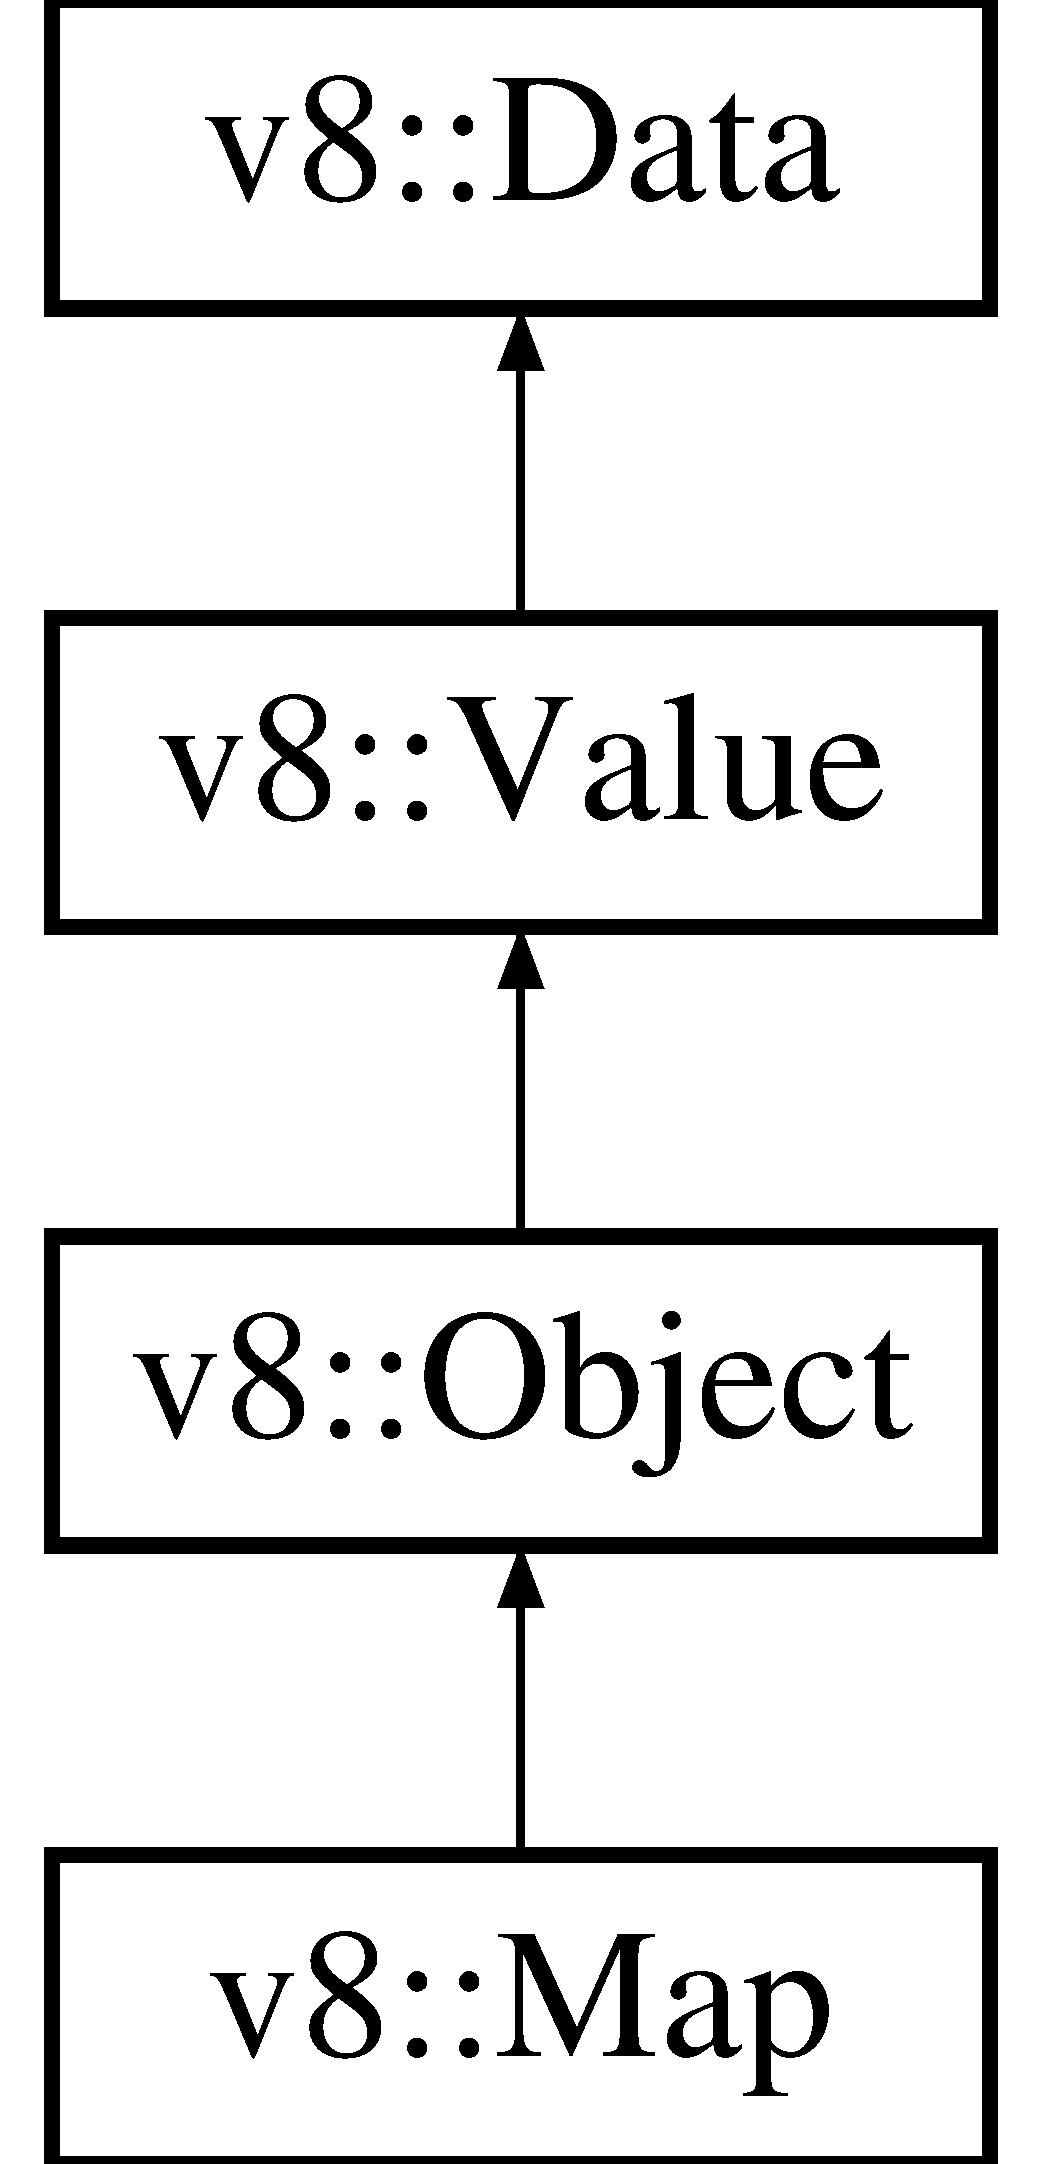
\includegraphics[height=4.000000cm]{classv8_1_1Map}
\end{center}
\end{figure}
\subsection*{Public Member Functions}
\begin{DoxyCompactItemize}
\item 
\mbox{\Hypertarget{classv8_1_1Map_a62cb76161d9a4a62a14e32b2f3f5b490}\label{classv8_1_1Map_a62cb76161d9a4a62a14e32b2f3f5b490}} 
size\+\_\+t {\bfseries Size} () const
\item 
\mbox{\Hypertarget{classv8_1_1Map_a06ee0d566d206058a7fe22c140000be4}\label{classv8_1_1Map_a06ee0d566d206058a7fe22c140000be4}} 
void {\bfseries Clear} ()
\item 
\mbox{\Hypertarget{classv8_1_1Map_a18b0a4d81e6900e854ceeabb516b5d72}\label{classv8_1_1Map_a18b0a4d81e6900e854ceeabb516b5d72}} 
V8\+\_\+\+W\+A\+R\+N\+\_\+\+U\+N\+U\+S\+E\+D\+\_\+\+R\+E\+S\+U\+LT \mbox{\hyperlink{classv8_1_1MaybeLocal}{Maybe\+Local}}$<$ \mbox{\hyperlink{classv8_1_1Value}{Value}} $>$ {\bfseries Get} (\mbox{\hyperlink{classv8_1_1Local}{Local}}$<$ Context $>$ context, \mbox{\hyperlink{classv8_1_1Local}{Local}}$<$ \mbox{\hyperlink{classv8_1_1Value}{Value}} $>$ key)
\item 
\mbox{\Hypertarget{classv8_1_1Map_a46f73b93abc9601a9a90e2051a64bcd3}\label{classv8_1_1Map_a46f73b93abc9601a9a90e2051a64bcd3}} 
V8\+\_\+\+W\+A\+R\+N\+\_\+\+U\+N\+U\+S\+E\+D\+\_\+\+R\+E\+S\+U\+LT \mbox{\hyperlink{classv8_1_1MaybeLocal}{Maybe\+Local}}$<$ \mbox{\hyperlink{classv8_1_1Map}{Map}} $>$ {\bfseries Set} (\mbox{\hyperlink{classv8_1_1Local}{Local}}$<$ Context $>$ context, \mbox{\hyperlink{classv8_1_1Local}{Local}}$<$ \mbox{\hyperlink{classv8_1_1Value}{Value}} $>$ key, \mbox{\hyperlink{classv8_1_1Local}{Local}}$<$ \mbox{\hyperlink{classv8_1_1Value}{Value}} $>$ value)
\item 
\mbox{\Hypertarget{classv8_1_1Map_abc50dbc81ed6f6eecdb552238b97182b}\label{classv8_1_1Map_abc50dbc81ed6f6eecdb552238b97182b}} 
V8\+\_\+\+W\+A\+R\+N\+\_\+\+U\+N\+U\+S\+E\+D\+\_\+\+R\+E\+S\+U\+LT \mbox{\hyperlink{classv8_1_1Maybe}{Maybe}}$<$ bool $>$ {\bfseries Has} (\mbox{\hyperlink{classv8_1_1Local}{Local}}$<$ Context $>$ context, \mbox{\hyperlink{classv8_1_1Local}{Local}}$<$ \mbox{\hyperlink{classv8_1_1Value}{Value}} $>$ key)
\item 
\mbox{\Hypertarget{classv8_1_1Map_a3e587498e1629ae10255f3c2a2beb9dc}\label{classv8_1_1Map_a3e587498e1629ae10255f3c2a2beb9dc}} 
V8\+\_\+\+W\+A\+R\+N\+\_\+\+U\+N\+U\+S\+E\+D\+\_\+\+R\+E\+S\+U\+LT \mbox{\hyperlink{classv8_1_1Maybe}{Maybe}}$<$ bool $>$ {\bfseries Delete} (\mbox{\hyperlink{classv8_1_1Local}{Local}}$<$ Context $>$ context, \mbox{\hyperlink{classv8_1_1Local}{Local}}$<$ \mbox{\hyperlink{classv8_1_1Value}{Value}} $>$ key)
\item 
\mbox{\hyperlink{classv8_1_1Local}{Local}}$<$ \mbox{\hyperlink{classv8_1_1Array}{Array}} $>$ \mbox{\hyperlink{classv8_1_1Map_a924483cc18fa2f287a43ca2d7eaef763}{As\+Array}} () const
\end{DoxyCompactItemize}
\subsection*{Static Public Member Functions}
\begin{DoxyCompactItemize}
\item 
static \mbox{\hyperlink{classv8_1_1Local}{Local}}$<$ \mbox{\hyperlink{classv8_1_1Map}{Map}} $>$ \mbox{\hyperlink{classv8_1_1Map_afeefcbe3b73ae398051d4b5bbb3f075d}{New}} (Isolate $\ast$isolate)
\item 
\mbox{\Hypertarget{classv8_1_1Map_ac53aafed02f275a7d3ce6da8cfd060c3}\label{classv8_1_1Map_ac53aafed02f275a7d3ce6da8cfd060c3}} 
static V8\+\_\+\+I\+N\+L\+I\+NE \mbox{\hyperlink{classv8_1_1Map}{Map}} $\ast$ {\bfseries Cast} (\mbox{\hyperlink{classv8_1_1Value}{Value}} $\ast$obj)
\end{DoxyCompactItemize}


\subsection{Detailed Description}
An instance of the built-\/in \mbox{\hyperlink{classv8_1_1Map}{Map}} constructor (E\+C\+M\+A-\/262, 6th Edition, 23.\+1.\+1). 

Definition at line 3704 of file v8.\+h.



\subsection{Member Function Documentation}
\mbox{\Hypertarget{classv8_1_1Map_a924483cc18fa2f287a43ca2d7eaef763}\label{classv8_1_1Map_a924483cc18fa2f287a43ca2d7eaef763}} 
\index{v8\+::\+Map@{v8\+::\+Map}!As\+Array@{As\+Array}}
\index{As\+Array@{As\+Array}!v8\+::\+Map@{v8\+::\+Map}}
\subsubsection{\texorpdfstring{As\+Array()}{AsArray()}}
{\footnotesize\ttfamily \mbox{\hyperlink{classv8_1_1Local}{Local}}$<$\mbox{\hyperlink{classv8_1_1Array}{Array}}$>$ v8\+::\+Map\+::\+As\+Array (\begin{DoxyParamCaption}{ }\end{DoxyParamCaption}) const}

Returns an array of length Size() $\ast$ 2, where index N is the Nth key and index N + 1 is the Nth value. \mbox{\Hypertarget{classv8_1_1Map_afeefcbe3b73ae398051d4b5bbb3f075d}\label{classv8_1_1Map_afeefcbe3b73ae398051d4b5bbb3f075d}} 
\index{v8\+::\+Map@{v8\+::\+Map}!New@{New}}
\index{New@{New}!v8\+::\+Map@{v8\+::\+Map}}
\subsubsection{\texorpdfstring{New()}{New()}}
{\footnotesize\ttfamily static \mbox{\hyperlink{classv8_1_1Local}{Local}}$<$\mbox{\hyperlink{classv8_1_1Map}{Map}}$>$ v8\+::\+Map\+::\+New (\begin{DoxyParamCaption}\item[{Isolate $\ast$}]{isolate }\end{DoxyParamCaption})\hspace{0.3cm}{\ttfamily [static]}}

Creates a new empty \mbox{\hyperlink{classv8_1_1Map}{Map}}. 

The documentation for this class was generated from the following file\+:\begin{DoxyCompactItemize}
\item 
v8/include/v8.\+h\end{DoxyCompactItemize}

\hypertarget{classv8_1_1Maybe}{}\section{v8\+:\+:Maybe$<$ T $>$ Class Template Reference}
\label{classv8_1_1Maybe}\index{v8\+::\+Maybe$<$ T $>$@{v8\+::\+Maybe$<$ T $>$}}


{\ttfamily \#include $<$v8.\+h$>$}

\subsection*{Public Member Functions}
\begin{DoxyCompactItemize}
\item 
\hypertarget{classv8_1_1Maybe_a486b608c21c8038d5019bd7d75866345}{}V8\+\_\+\+I\+N\+L\+I\+N\+E bool {\bfseries Is\+Nothing} () const \label{classv8_1_1Maybe_a486b608c21c8038d5019bd7d75866345}

\item 
\hypertarget{classv8_1_1Maybe_adc82dc945891060d312fb6fbf8fb56ae}{}V8\+\_\+\+I\+N\+L\+I\+N\+E bool {\bfseries Is\+Just} () const \label{classv8_1_1Maybe_adc82dc945891060d312fb6fbf8fb56ae}

\item 
\hypertarget{classv8_1_1Maybe_a02b19d7fcb7744d8dba3530ef8e14c8c}{}V8\+\_\+\+I\+N\+L\+I\+N\+E T {\bfseries From\+Just} () const \label{classv8_1_1Maybe_a02b19d7fcb7744d8dba3530ef8e14c8c}

\item 
\hypertarget{classv8_1_1Maybe_a0bcb5fb0d0e92a3f0cc546f11068a8df}{}V8\+\_\+\+I\+N\+L\+I\+N\+E T {\bfseries From\+Maybe} (const T \&default\+\_\+value) const \label{classv8_1_1Maybe_a0bcb5fb0d0e92a3f0cc546f11068a8df}

\item 
\hypertarget{classv8_1_1Maybe_adf61111c2da44e10ba5ab546a9a525ce}{}V8\+\_\+\+I\+N\+L\+I\+N\+E bool {\bfseries operator==} (const \hyperlink{classv8_1_1Maybe}{Maybe} \&other) const \label{classv8_1_1Maybe_adf61111c2da44e10ba5ab546a9a525ce}

\item 
\hypertarget{classv8_1_1Maybe_a5bbacc606422d7ab327c2683462342ec}{}V8\+\_\+\+I\+N\+L\+I\+N\+E bool {\bfseries operator!=} (const \hyperlink{classv8_1_1Maybe}{Maybe} \&other) const \label{classv8_1_1Maybe_a5bbacc606422d7ab327c2683462342ec}

\end{DoxyCompactItemize}
\subsection*{Friends}
\begin{DoxyCompactItemize}
\item 
\hypertarget{classv8_1_1Maybe_aeb9593e125b42d748acbd69b72c89f37}{}{\footnotesize template$<$class U $>$ }\\\hyperlink{classv8_1_1Maybe}{Maybe}$<$ U $>$ {\bfseries Nothing} ()\label{classv8_1_1Maybe_aeb9593e125b42d748acbd69b72c89f37}

\item 
\hypertarget{classv8_1_1Maybe_aeff0e7fedd63cfebe9a5286e2cd8552d}{}{\footnotesize template$<$class U $>$ }\\\hyperlink{classv8_1_1Maybe}{Maybe}$<$ U $>$ {\bfseries Just} (const U \&u)\label{classv8_1_1Maybe_aeff0e7fedd63cfebe9a5286e2cd8552d}

\end{DoxyCompactItemize}


\subsection{Detailed Description}
\subsubsection*{template$<$class T$>$class v8\+::\+Maybe$<$ T $>$}

A simple \hyperlink{classv8_1_1Maybe}{Maybe} type, representing an object which may or may not have a value, see \href{https://hackage.haskell.org/package/base/docs/Data-Maybe.html}{\tt https\+://hackage.\+haskell.\+org/package/base/docs/\+Data-\/\+Maybe.\+html}.

If an A\+P\+I method returns a Maybe$<$$>$, the A\+P\+I method can potentially fail either because an exception is thrown, or because an exception is pending, e.\+g. because a previous A\+P\+I call threw an exception that hasn\textquotesingle{}t been caught yet, or because a Terminate\+Execution exception was thrown. In that case, a \char`\"{}\+Nothing\char`\"{} value is returned. 

The documentation for this class was generated from the following file\+:\begin{DoxyCompactItemize}
\item 
v8/include/v8.\+h\end{DoxyCompactItemize}

\hypertarget{classv8_1_1MaybeLocal}{}\section{v8\+:\+:Maybe\+Local$<$ T $>$ Class Template Reference}
\label{classv8_1_1MaybeLocal}\index{v8\+::\+Maybe\+Local$<$ T $>$@{v8\+::\+Maybe\+Local$<$ T $>$}}


{\ttfamily \#include $<$v8.\+h$>$}

\subsection*{Public Member Functions}
\begin{DoxyCompactItemize}
\item 
\mbox{\Hypertarget{classv8_1_1MaybeLocal_ab488843c2faf4375517616d3c66886e5}\label{classv8_1_1MaybeLocal_ab488843c2faf4375517616d3c66886e5}} 
{\footnotesize template$<$class S $>$ }\\V8\+\_\+\+I\+N\+L\+I\+NE {\bfseries Maybe\+Local} (\mbox{\hyperlink{classv8_1_1Local}{Local}}$<$ S $>$ that)
\item 
\mbox{\Hypertarget{classv8_1_1MaybeLocal_aa321cd3ec18e64d893bc14b21e4624f4}\label{classv8_1_1MaybeLocal_aa321cd3ec18e64d893bc14b21e4624f4}} 
V8\+\_\+\+I\+N\+L\+I\+NE bool {\bfseries Is\+Empty} () const
\item 
{\footnotesize template$<$class S $>$ }\\V8\+\_\+\+W\+A\+R\+N\+\_\+\+U\+N\+U\+S\+E\+D\+\_\+\+R\+E\+S\+U\+LT V8\+\_\+\+I\+N\+L\+I\+NE bool \mbox{\hyperlink{classv8_1_1MaybeLocal_aa12fc83adccbf02f502a2aaeed9c32ab}{To\+Local}} (\mbox{\hyperlink{classv8_1_1Local}{Local}}$<$ S $>$ $\ast$out) const
\item 
V8\+\_\+\+I\+N\+L\+I\+NE \mbox{\hyperlink{classv8_1_1Local}{Local}}$<$ T $>$ \mbox{\hyperlink{classv8_1_1MaybeLocal_a9b2c9d50fca5897e3a03fd4c25d12415}{To\+Local\+Checked}} ()
\item 
{\footnotesize template$<$class S $>$ }\\V8\+\_\+\+I\+N\+L\+I\+NE \mbox{\hyperlink{classv8_1_1Local}{Local}}$<$ S $>$ \mbox{\hyperlink{classv8_1_1MaybeLocal_ad99cb1e7ac1a4eac34c144faa4262407}{From\+Maybe}} (\mbox{\hyperlink{classv8_1_1Local}{Local}}$<$ S $>$ default\+\_\+value) const
\end{DoxyCompactItemize}


\subsection{Detailed Description}
\subsubsection*{template$<$class T$>$\newline
class v8\+::\+Maybe\+Local$<$ T $>$}

A Maybe\+Local$<$$>$ is a wrapper around Local$<$$>$ that enforces a check whether the Local$<$$>$ is empty before it can be used.

If an A\+PI method returns a Maybe\+Local$<$$>$, the A\+PI method can potentially fail either because an exception is thrown, or because an exception is pending, e.\+g. because a previous A\+PI call threw an exception that hasn\textquotesingle{}t been caught yet, or because a Terminate\+Execution exception was thrown. In that case, an empty \mbox{\hyperlink{classv8_1_1MaybeLocal}{Maybe\+Local}} is returned. 

\subsection{Member Function Documentation}
\mbox{\Hypertarget{classv8_1_1MaybeLocal_ad99cb1e7ac1a4eac34c144faa4262407}\label{classv8_1_1MaybeLocal_ad99cb1e7ac1a4eac34c144faa4262407}} 
\index{v8\+::\+Maybe\+Local@{v8\+::\+Maybe\+Local}!From\+Maybe@{From\+Maybe}}
\index{From\+Maybe@{From\+Maybe}!v8\+::\+Maybe\+Local@{v8\+::\+Maybe\+Local}}
\subsubsection{\texorpdfstring{From\+Maybe()}{FromMaybe()}}
{\footnotesize\ttfamily template$<$class T $>$ \\
template$<$class S $>$ \\
V8\+\_\+\+I\+N\+L\+I\+NE \mbox{\hyperlink{classv8_1_1Local}{Local}}$<$S$>$ \mbox{\hyperlink{classv8_1_1MaybeLocal}{v8\+::\+Maybe\+Local}}$<$ T $>$\+::From\+Maybe (\begin{DoxyParamCaption}\item[{\mbox{\hyperlink{classv8_1_1Local}{Local}}$<$ S $>$}]{default\+\_\+value }\end{DoxyParamCaption}) const\hspace{0.3cm}{\ttfamily [inline]}}

Converts this Maybe\+Local$<$$>$ to a Local$<$$>$, using a default value if this Maybe\+Local$<$$>$ is empty. \mbox{\Hypertarget{classv8_1_1MaybeLocal_aa12fc83adccbf02f502a2aaeed9c32ab}\label{classv8_1_1MaybeLocal_aa12fc83adccbf02f502a2aaeed9c32ab}} 
\index{v8\+::\+Maybe\+Local@{v8\+::\+Maybe\+Local}!To\+Local@{To\+Local}}
\index{To\+Local@{To\+Local}!v8\+::\+Maybe\+Local@{v8\+::\+Maybe\+Local}}
\subsubsection{\texorpdfstring{To\+Local()}{ToLocal()}}
{\footnotesize\ttfamily template$<$class T $>$ \\
template$<$class S $>$ \\
V8\+\_\+\+W\+A\+R\+N\+\_\+\+U\+N\+U\+S\+E\+D\+\_\+\+R\+E\+S\+U\+LT V8\+\_\+\+I\+N\+L\+I\+NE bool \mbox{\hyperlink{classv8_1_1MaybeLocal}{v8\+::\+Maybe\+Local}}$<$ T $>$\+::To\+Local (\begin{DoxyParamCaption}\item[{\mbox{\hyperlink{classv8_1_1Local}{Local}}$<$ S $>$ $\ast$}]{out }\end{DoxyParamCaption}) const\hspace{0.3cm}{\ttfamily [inline]}}

Converts this Maybe\+Local$<$$>$ to a Local$<$$>$. If this Maybe\+Local$<$$>$ is empty, $\vert$false$\vert$ is returned and $\vert$out$\vert$ is left untouched. \mbox{\Hypertarget{classv8_1_1MaybeLocal_a9b2c9d50fca5897e3a03fd4c25d12415}\label{classv8_1_1MaybeLocal_a9b2c9d50fca5897e3a03fd4c25d12415}} 
\index{v8\+::\+Maybe\+Local@{v8\+::\+Maybe\+Local}!To\+Local\+Checked@{To\+Local\+Checked}}
\index{To\+Local\+Checked@{To\+Local\+Checked}!v8\+::\+Maybe\+Local@{v8\+::\+Maybe\+Local}}
\subsubsection{\texorpdfstring{To\+Local\+Checked()}{ToLocalChecked()}}
{\footnotesize\ttfamily template$<$class T $>$ \\
\mbox{\hyperlink{classv8_1_1Local}{Local}}$<$ T $>$ \mbox{\hyperlink{classv8_1_1MaybeLocal}{v8\+::\+Maybe\+Local}}$<$ T $>$\+::To\+Local\+Checked (\begin{DoxyParamCaption}{ }\end{DoxyParamCaption})}

Converts this Maybe\+Local$<$$>$ to a Local$<$$>$. If this Maybe\+Local$<$$>$ is empty, V8 will crash the process. 

The documentation for this class was generated from the following file\+:\begin{DoxyCompactItemize}
\item 
v8/include/v8.\+h\end{DoxyCompactItemize}

\hypertarget{classv8_1_1Debug_1_1Message}{}\section{v8\+:\+:Debug\+:\+:Message Class Reference}
\label{classv8_1_1Debug_1_1Message}\index{v8\+::\+Debug\+::\+Message@{v8\+::\+Debug\+::\+Message}}


{\ttfamily \#include $<$v8-\/debug.\+h$>$}

\subsection*{Public Member Functions}
\begin{DoxyCompactItemize}
\item 
virtual bool \hyperlink{classv8_1_1Debug_1_1Message_a36ade83a9c960ce581b1a4051f763785}{Is\+Event} () const =0
\item 
\hypertarget{classv8_1_1Debug_1_1Message_a1d65d6efbb5adb96406f7e285bb25ee3}{}virtual bool {\bfseries Is\+Response} () const =0\label{classv8_1_1Debug_1_1Message_a1d65d6efbb5adb96406f7e285bb25ee3}

\item 
\hypertarget{classv8_1_1Debug_1_1Message_a8a99a5c9fe0db14fbaccaed297d9c203}{}virtual Debug\+Event {\bfseries Get\+Event} () const =0\label{classv8_1_1Debug_1_1Message_a8a99a5c9fe0db14fbaccaed297d9c203}

\item 
virtual bool \hyperlink{classv8_1_1Debug_1_1Message_af8d236b6a334423732a38cbf8cfd7aef}{Will\+Start\+Running} () const =0
\item 
virtual \hyperlink{classv8_1_1Local}{Local}$<$ \hyperlink{classv8_1_1Object}{Object} $>$ \hyperlink{classv8_1_1Debug_1_1Message_a0e20677046473f0bdcdc8656cdff1651}{Get\+Execution\+State} () const =0
\item 
\hypertarget{classv8_1_1Debug_1_1Message_a4c06f55aec5aba3eb10f2b284545ea13}{}virtual \hyperlink{classv8_1_1Local}{Local}$<$ \hyperlink{classv8_1_1Object}{Object} $>$ {\bfseries Get\+Event\+Data} () const =0\label{classv8_1_1Debug_1_1Message_a4c06f55aec5aba3eb10f2b284545ea13}

\item 
virtual \hyperlink{classv8_1_1Local}{Local}$<$ \hyperlink{classv8_1_1String}{String} $>$ \hyperlink{classv8_1_1Debug_1_1Message_ad1cc300c42a92890bfab4122fa657ea5}{Get\+J\+S\+O\+N} () const =0
\item 
virtual \hyperlink{classv8_1_1Local}{Local}$<$ \hyperlink{classv8_1_1Context}{Context} $>$ \hyperlink{classv8_1_1Debug_1_1Message_ab6632d15830b5c5f474a4da36405478d}{Get\+Event\+Context} () const =0
\item 
virtual \hyperlink{classv8_1_1Debug_1_1ClientData}{Client\+Data} $\ast$ \hyperlink{classv8_1_1Debug_1_1Message_ab81bb81d233f5f37e6626a7bcac22142}{Get\+Client\+Data} () const =0
\item 
\hypertarget{classv8_1_1Debug_1_1Message_a71b3624e8f851108330d6b64bbb611f5}{}virtual \hyperlink{classv8_1_1Isolate}{Isolate} $\ast$ {\bfseries Get\+Isolate} () const =0\label{classv8_1_1Debug_1_1Message_a71b3624e8f851108330d6b64bbb611f5}

\end{DoxyCompactItemize}


\subsection{Detailed Description}
A message object passed to the debug message handler. 

\subsection{Member Function Documentation}
\hypertarget{classv8_1_1Debug_1_1Message_ab81bb81d233f5f37e6626a7bcac22142}{}\index{v8\+::\+Debug\+::\+Message@{v8\+::\+Debug\+::\+Message}!Get\+Client\+Data@{Get\+Client\+Data}}
\index{Get\+Client\+Data@{Get\+Client\+Data}!v8\+::\+Debug\+::\+Message@{v8\+::\+Debug\+::\+Message}}
\subsubsection[{Get\+Client\+Data}]{\setlength{\rightskip}{0pt plus 5cm}virtual {\bf Client\+Data}$\ast$ v8\+::\+Debug\+::\+Message\+::\+Get\+Client\+Data (
\begin{DoxyParamCaption}
{}
\end{DoxyParamCaption}
) const\hspace{0.3cm}{\ttfamily [pure virtual]}}\label{classv8_1_1Debug_1_1Message_ab81bb81d233f5f37e6626a7bcac22142}
Client data passed with the corresponding request if any. This is the client\+\_\+data data value passed into Debug\+::\+Send\+Command along with the request that led to the message or N\+U\+L\+L if the message is an event. The debugger takes ownership of the data and will delete it even if there is no message handler. \hypertarget{classv8_1_1Debug_1_1Message_ab6632d15830b5c5f474a4da36405478d}{}\index{v8\+::\+Debug\+::\+Message@{v8\+::\+Debug\+::\+Message}!Get\+Event\+Context@{Get\+Event\+Context}}
\index{Get\+Event\+Context@{Get\+Event\+Context}!v8\+::\+Debug\+::\+Message@{v8\+::\+Debug\+::\+Message}}
\subsubsection[{Get\+Event\+Context}]{\setlength{\rightskip}{0pt plus 5cm}virtual {\bf Local}$<${\bf Context}$>$ v8\+::\+Debug\+::\+Message\+::\+Get\+Event\+Context (
\begin{DoxyParamCaption}
{}
\end{DoxyParamCaption}
) const\hspace{0.3cm}{\ttfamily [pure virtual]}}\label{classv8_1_1Debug_1_1Message_ab6632d15830b5c5f474a4da36405478d}
Get the context active when the debug event happened. Note this is not the current active context as the Java\+Script part of the debugger is running in its own context which is entered at this point. \hypertarget{classv8_1_1Debug_1_1Message_a0e20677046473f0bdcdc8656cdff1651}{}\index{v8\+::\+Debug\+::\+Message@{v8\+::\+Debug\+::\+Message}!Get\+Execution\+State@{Get\+Execution\+State}}
\index{Get\+Execution\+State@{Get\+Execution\+State}!v8\+::\+Debug\+::\+Message@{v8\+::\+Debug\+::\+Message}}
\subsubsection[{Get\+Execution\+State}]{\setlength{\rightskip}{0pt plus 5cm}virtual {\bf Local}$<${\bf Object}$>$ v8\+::\+Debug\+::\+Message\+::\+Get\+Execution\+State (
\begin{DoxyParamCaption}
{}
\end{DoxyParamCaption}
) const\hspace{0.3cm}{\ttfamily [pure virtual]}}\label{classv8_1_1Debug_1_1Message_a0e20677046473f0bdcdc8656cdff1651}
Access to execution state and event data. Don\textquotesingle{}t store these cross callbacks as their content becomes invalid. These objects are from the debugger event that started the debug message loop. \hypertarget{classv8_1_1Debug_1_1Message_ad1cc300c42a92890bfab4122fa657ea5}{}\index{v8\+::\+Debug\+::\+Message@{v8\+::\+Debug\+::\+Message}!Get\+J\+S\+O\+N@{Get\+J\+S\+O\+N}}
\index{Get\+J\+S\+O\+N@{Get\+J\+S\+O\+N}!v8\+::\+Debug\+::\+Message@{v8\+::\+Debug\+::\+Message}}
\subsubsection[{Get\+J\+S\+O\+N}]{\setlength{\rightskip}{0pt plus 5cm}virtual {\bf Local}$<${\bf String}$>$ v8\+::\+Debug\+::\+Message\+::\+Get\+J\+S\+O\+N (
\begin{DoxyParamCaption}
{}
\end{DoxyParamCaption}
) const\hspace{0.3cm}{\ttfamily [pure virtual]}}\label{classv8_1_1Debug_1_1Message_ad1cc300c42a92890bfab4122fa657ea5}
Get the debugger protocol \hyperlink{classv8_1_1JSON}{J\+S\+O\+N}. \hypertarget{classv8_1_1Debug_1_1Message_a36ade83a9c960ce581b1a4051f763785}{}\index{v8\+::\+Debug\+::\+Message@{v8\+::\+Debug\+::\+Message}!Is\+Event@{Is\+Event}}
\index{Is\+Event@{Is\+Event}!v8\+::\+Debug\+::\+Message@{v8\+::\+Debug\+::\+Message}}
\subsubsection[{Is\+Event}]{\setlength{\rightskip}{0pt plus 5cm}virtual bool v8\+::\+Debug\+::\+Message\+::\+Is\+Event (
\begin{DoxyParamCaption}
{}
\end{DoxyParamCaption}
) const\hspace{0.3cm}{\ttfamily [pure virtual]}}\label{classv8_1_1Debug_1_1Message_a36ade83a9c960ce581b1a4051f763785}
Check type of message. \hypertarget{classv8_1_1Debug_1_1Message_af8d236b6a334423732a38cbf8cfd7aef}{}\index{v8\+::\+Debug\+::\+Message@{v8\+::\+Debug\+::\+Message}!Will\+Start\+Running@{Will\+Start\+Running}}
\index{Will\+Start\+Running@{Will\+Start\+Running}!v8\+::\+Debug\+::\+Message@{v8\+::\+Debug\+::\+Message}}
\subsubsection[{Will\+Start\+Running}]{\setlength{\rightskip}{0pt plus 5cm}virtual bool v8\+::\+Debug\+::\+Message\+::\+Will\+Start\+Running (
\begin{DoxyParamCaption}
{}
\end{DoxyParamCaption}
) const\hspace{0.3cm}{\ttfamily [pure virtual]}}\label{classv8_1_1Debug_1_1Message_af8d236b6a334423732a38cbf8cfd7aef}
Indicate whether this is a response to a continue command which will start the V\+M running after this is processed. 

The documentation for this class was generated from the following file\+:\begin{DoxyCompactItemize}
\item 
v8/include/v8-\/debug.\+h\end{DoxyCompactItemize}

\hypertarget{classv8_1_1Message}{}\section{v8\+:\+:Message Class Reference}
\label{classv8_1_1Message}\index{v8\+::\+Message@{v8\+::\+Message}}


{\ttfamily \#include $<$v8.\+h$>$}

\subsection*{Public Member Functions}
\begin{DoxyCompactItemize}
\item 
\hypertarget{classv8_1_1Message_a72f26c7b684bbfbd14d5970849fdf3d2}{}\hyperlink{classv8_1_1Local}{Local}$<$ \hyperlink{classv8_1_1String}{String} $>$ {\bfseries Get} () const \label{classv8_1_1Message_a72f26c7b684bbfbd14d5970849fdf3d2}

\item 
\hypertarget{classv8_1_1Message_abcb8b2005ba077d855c4fcf775151fd6}{}{\bfseries V8\+\_\+\+D\+E\+P\+R\+E\+C\+A\+T\+E\+\_\+\+S\+O\+O\+N} (\char`\"{}Use maybe version\char`\"{}, Local$<$ \hyperlink{classv8_1_1String}{String} $>$ Get\+Source\+Line() const)\label{classv8_1_1Message_abcb8b2005ba077d855c4fcf775151fd6}

\item 
\hypertarget{classv8_1_1Message_a036059b3f15a98f9814f470b65948956}{}V8\+\_\+\+W\+A\+R\+N\+\_\+\+U\+N\+U\+S\+E\+D\+\_\+\+R\+E\+S\+U\+L\+T \hyperlink{classv8_1_1MaybeLocal}{Maybe\+Local}$<$ \hyperlink{classv8_1_1String}{String} $>$ {\bfseries Get\+Source\+Line} (\hyperlink{classv8_1_1Local}{Local}$<$ \hyperlink{classv8_1_1Context}{Context} $>$ context) const \label{classv8_1_1Message_a036059b3f15a98f9814f470b65948956}

\item 
\hyperlink{classv8_1_1ScriptOrigin}{Script\+Origin} \hyperlink{classv8_1_1Message_ae0fc442f44bd2b600c4d89a50cf3abd9}{Get\+Script\+Origin} () const 
\item 
\hyperlink{classv8_1_1Local}{Local}$<$ \hyperlink{classv8_1_1Value}{Value} $>$ \hyperlink{classv8_1_1Message_a66200e721dc4aa00568099ba67e9143a}{Get\+Script\+Resource\+Name} () const 
\item 
\hyperlink{classv8_1_1Local}{Local}$<$ \hyperlink{classv8_1_1StackTrace}{Stack\+Trace} $>$ \hyperlink{classv8_1_1Message_a42738680a1f28c495010a76b73373445}{Get\+Stack\+Trace} () const 
\item 
\hyperlink{classv8_1_1Message_a0a6855ef9eda008aa0f06f8cdf2a41e4}{V8\+\_\+\+D\+E\+P\+R\+E\+C\+A\+T\+E\+\_\+\+S\+O\+O\+N} (\char`\"{}Use maybe version\char`\"{}, int Get\+Line\+Number() const)
\item 
\hypertarget{classv8_1_1Message_a9425c8d1b3f7e3a066458c676642c6df}{}V8\+\_\+\+W\+A\+R\+N\+\_\+\+U\+N\+U\+S\+E\+D\+\_\+\+R\+E\+S\+U\+L\+T \hyperlink{classv8_1_1Maybe}{Maybe}$<$ int $>$ {\bfseries Get\+Line\+Number} (\hyperlink{classv8_1_1Local}{Local}$<$ \hyperlink{classv8_1_1Context}{Context} $>$ context) const \label{classv8_1_1Message_a9425c8d1b3f7e3a066458c676642c6df}

\item 
int \hyperlink{classv8_1_1Message_a31a550a1d3d09a2d72d0742be821956f}{Get\+Start\+Position} () const 
\item 
int \hyperlink{classv8_1_1Message_a50cbec87379e628b1647466926882037}{Get\+End\+Position} () const 
\item 
\hyperlink{classv8_1_1Message_a4715c868bd87bbc65a74c8aca27ec692}{V8\+\_\+\+D\+E\+P\+R\+E\+C\+A\+T\+E\+\_\+\+S\+O\+O\+N} (\char`\"{}Use maybe version\char`\"{}, int Get\+Start\+Column() const)
\item 
\hypertarget{classv8_1_1Message_aedffb63ec9761af77b9492351b0bd8a2}{}V8\+\_\+\+W\+A\+R\+N\+\_\+\+U\+N\+U\+S\+E\+D\+\_\+\+R\+E\+S\+U\+L\+T \hyperlink{classv8_1_1Maybe}{Maybe}$<$ int $>$ {\bfseries Get\+Start\+Column} (\hyperlink{classv8_1_1Local}{Local}$<$ \hyperlink{classv8_1_1Context}{Context} $>$ context) const \label{classv8_1_1Message_aedffb63ec9761af77b9492351b0bd8a2}

\item 
\hyperlink{classv8_1_1Message_a9290b52ab2eaebc65fe44b432fc58766}{V8\+\_\+\+D\+E\+P\+R\+E\+C\+A\+T\+E\+\_\+\+S\+O\+O\+N} (\char`\"{}Use maybe version\char`\"{}, int Get\+End\+Column() const)
\item 
\hypertarget{classv8_1_1Message_aa6f918e778dd9ad173dbdfa75c9f614f}{}V8\+\_\+\+W\+A\+R\+N\+\_\+\+U\+N\+U\+S\+E\+D\+\_\+\+R\+E\+S\+U\+L\+T \hyperlink{classv8_1_1Maybe}{Maybe}$<$ int $>$ {\bfseries Get\+End\+Column} (\hyperlink{classv8_1_1Local}{Local}$<$ \hyperlink{classv8_1_1Context}{Context} $>$ context) const \label{classv8_1_1Message_aa6f918e778dd9ad173dbdfa75c9f614f}

\item 
bool \hyperlink{classv8_1_1Message_a03228f50c40c45da52f424bdd64598d1}{Is\+Shared\+Cross\+Origin} () const 
\item 
\hypertarget{classv8_1_1Message_a2ab104d29e13bc942f345e09472ed531}{}bool {\bfseries Is\+Opaque} () const \label{classv8_1_1Message_a2ab104d29e13bc942f345e09472ed531}

\end{DoxyCompactItemize}
\subsection*{Static Public Member Functions}
\begin{DoxyCompactItemize}
\item 
\hypertarget{classv8_1_1Message_ae5d67d123c5611e6bc36824c938cbfa5}{}static void {\bfseries Print\+Current\+Stack\+Trace} (\hyperlink{classv8_1_1Isolate}{Isolate} $\ast$isolate, F\+I\+L\+E $\ast$out)\label{classv8_1_1Message_ae5d67d123c5611e6bc36824c938cbfa5}

\end{DoxyCompactItemize}
\subsection*{Static Public Attributes}
\begin{DoxyCompactItemize}
\item 
\hypertarget{classv8_1_1Message_a35649a6c0c813ba82c9886a2b17da124}{}static const int {\bfseries k\+No\+Line\+Number\+Info} = 0\label{classv8_1_1Message_a35649a6c0c813ba82c9886a2b17da124}

\item 
\hypertarget{classv8_1_1Message_a8cb643dbf408b0fd2526b23a8202c4a6}{}static const int {\bfseries k\+No\+Column\+Info} = 0\label{classv8_1_1Message_a8cb643dbf408b0fd2526b23a8202c4a6}

\item 
\hypertarget{classv8_1_1Message_a5aac643173466e88544cb1daa74553d6}{}static const int {\bfseries k\+No\+Script\+Id\+Info} = 0\label{classv8_1_1Message_a5aac643173466e88544cb1daa74553d6}

\end{DoxyCompactItemize}


\subsection{Detailed Description}
An error message. 

\subsection{Member Function Documentation}
\hypertarget{classv8_1_1Message_a50cbec87379e628b1647466926882037}{}\index{v8\+::\+Message@{v8\+::\+Message}!Get\+End\+Position@{Get\+End\+Position}}
\index{Get\+End\+Position@{Get\+End\+Position}!v8\+::\+Message@{v8\+::\+Message}}
\subsubsection[{Get\+End\+Position}]{\setlength{\rightskip}{0pt plus 5cm}int v8\+::\+Message\+::\+Get\+End\+Position (
\begin{DoxyParamCaption}
{}
\end{DoxyParamCaption}
) const}\label{classv8_1_1Message_a50cbec87379e628b1647466926882037}
Returns the index within the script of the last character where the error occurred. \hypertarget{classv8_1_1Message_ae0fc442f44bd2b600c4d89a50cf3abd9}{}\index{v8\+::\+Message@{v8\+::\+Message}!Get\+Script\+Origin@{Get\+Script\+Origin}}
\index{Get\+Script\+Origin@{Get\+Script\+Origin}!v8\+::\+Message@{v8\+::\+Message}}
\subsubsection[{Get\+Script\+Origin}]{\setlength{\rightskip}{0pt plus 5cm}{\bf Script\+Origin} v8\+::\+Message\+::\+Get\+Script\+Origin (
\begin{DoxyParamCaption}
{}
\end{DoxyParamCaption}
) const}\label{classv8_1_1Message_ae0fc442f44bd2b600c4d89a50cf3abd9}
Returns the origin for the script from where the function causing the error originates. \hypertarget{classv8_1_1Message_a66200e721dc4aa00568099ba67e9143a}{}\index{v8\+::\+Message@{v8\+::\+Message}!Get\+Script\+Resource\+Name@{Get\+Script\+Resource\+Name}}
\index{Get\+Script\+Resource\+Name@{Get\+Script\+Resource\+Name}!v8\+::\+Message@{v8\+::\+Message}}
\subsubsection[{Get\+Script\+Resource\+Name}]{\setlength{\rightskip}{0pt plus 5cm}{\bf Local}$<${\bf Value}$>$ v8\+::\+Message\+::\+Get\+Script\+Resource\+Name (
\begin{DoxyParamCaption}
{}
\end{DoxyParamCaption}
) const}\label{classv8_1_1Message_a66200e721dc4aa00568099ba67e9143a}
Returns the resource name for the script from where the function causing the error originates. \hypertarget{classv8_1_1Message_a42738680a1f28c495010a76b73373445}{}\index{v8\+::\+Message@{v8\+::\+Message}!Get\+Stack\+Trace@{Get\+Stack\+Trace}}
\index{Get\+Stack\+Trace@{Get\+Stack\+Trace}!v8\+::\+Message@{v8\+::\+Message}}
\subsubsection[{Get\+Stack\+Trace}]{\setlength{\rightskip}{0pt plus 5cm}{\bf Local}$<${\bf Stack\+Trace}$>$ v8\+::\+Message\+::\+Get\+Stack\+Trace (
\begin{DoxyParamCaption}
{}
\end{DoxyParamCaption}
) const}\label{classv8_1_1Message_a42738680a1f28c495010a76b73373445}
\hyperlink{classv8_1_1Exception}{Exception} stack trace. By default stack traces are not captured for uncaught exceptions. Set\+Capture\+Stack\+Trace\+For\+Uncaught\+Exceptions allows to change this option. \hypertarget{classv8_1_1Message_a31a550a1d3d09a2d72d0742be821956f}{}\index{v8\+::\+Message@{v8\+::\+Message}!Get\+Start\+Position@{Get\+Start\+Position}}
\index{Get\+Start\+Position@{Get\+Start\+Position}!v8\+::\+Message@{v8\+::\+Message}}
\subsubsection[{Get\+Start\+Position}]{\setlength{\rightskip}{0pt plus 5cm}int v8\+::\+Message\+::\+Get\+Start\+Position (
\begin{DoxyParamCaption}
{}
\end{DoxyParamCaption}
) const}\label{classv8_1_1Message_a31a550a1d3d09a2d72d0742be821956f}
Returns the index within the script of the first character where the error occurred. \hypertarget{classv8_1_1Message_a03228f50c40c45da52f424bdd64598d1}{}\index{v8\+::\+Message@{v8\+::\+Message}!Is\+Shared\+Cross\+Origin@{Is\+Shared\+Cross\+Origin}}
\index{Is\+Shared\+Cross\+Origin@{Is\+Shared\+Cross\+Origin}!v8\+::\+Message@{v8\+::\+Message}}
\subsubsection[{Is\+Shared\+Cross\+Origin}]{\setlength{\rightskip}{0pt plus 5cm}bool v8\+::\+Message\+::\+Is\+Shared\+Cross\+Origin (
\begin{DoxyParamCaption}
{}
\end{DoxyParamCaption}
) const}\label{classv8_1_1Message_a03228f50c40c45da52f424bdd64598d1}
Passes on the value set by the embedder when it fed the script from which this \hyperlink{classv8_1_1Message}{Message} was generated to \hyperlink{classv8_1_1V8}{V8}. \hypertarget{classv8_1_1Message_a0a6855ef9eda008aa0f06f8cdf2a41e4}{}\index{v8\+::\+Message@{v8\+::\+Message}!V8\+\_\+\+D\+E\+P\+R\+E\+C\+A\+T\+E\+\_\+\+S\+O\+O\+N@{V8\+\_\+\+D\+E\+P\+R\+E\+C\+A\+T\+E\+\_\+\+S\+O\+O\+N}}
\index{V8\+\_\+\+D\+E\+P\+R\+E\+C\+A\+T\+E\+\_\+\+S\+O\+O\+N@{V8\+\_\+\+D\+E\+P\+R\+E\+C\+A\+T\+E\+\_\+\+S\+O\+O\+N}!v8\+::\+Message@{v8\+::\+Message}}
\subsubsection[{V8\+\_\+\+D\+E\+P\+R\+E\+C\+A\+T\+E\+\_\+\+S\+O\+O\+N}]{\setlength{\rightskip}{0pt plus 5cm}v8\+::\+Message\+::\+V8\+\_\+\+D\+E\+P\+R\+E\+C\+A\+T\+E\+\_\+\+S\+O\+O\+N (
\begin{DoxyParamCaption}
\item[{\char`\"{}Use maybe version\char`\"{}}]{, }
\item[{int Get\+Line\+Number()}]{const}
\end{DoxyParamCaption}
)}\label{classv8_1_1Message_a0a6855ef9eda008aa0f06f8cdf2a41e4}
Returns the number, 1-\/based, of the line where the error occurred. \hypertarget{classv8_1_1Message_a4715c868bd87bbc65a74c8aca27ec692}{}\index{v8\+::\+Message@{v8\+::\+Message}!V8\+\_\+\+D\+E\+P\+R\+E\+C\+A\+T\+E\+\_\+\+S\+O\+O\+N@{V8\+\_\+\+D\+E\+P\+R\+E\+C\+A\+T\+E\+\_\+\+S\+O\+O\+N}}
\index{V8\+\_\+\+D\+E\+P\+R\+E\+C\+A\+T\+E\+\_\+\+S\+O\+O\+N@{V8\+\_\+\+D\+E\+P\+R\+E\+C\+A\+T\+E\+\_\+\+S\+O\+O\+N}!v8\+::\+Message@{v8\+::\+Message}}
\subsubsection[{V8\+\_\+\+D\+E\+P\+R\+E\+C\+A\+T\+E\+\_\+\+S\+O\+O\+N}]{\setlength{\rightskip}{0pt plus 5cm}v8\+::\+Message\+::\+V8\+\_\+\+D\+E\+P\+R\+E\+C\+A\+T\+E\+\_\+\+S\+O\+O\+N (
\begin{DoxyParamCaption}
\item[{\char`\"{}Use maybe version\char`\"{}}]{, }
\item[{int Get\+Start\+Column()}]{const}
\end{DoxyParamCaption}
)}\label{classv8_1_1Message_a4715c868bd87bbc65a74c8aca27ec692}
Returns the index within the line of the first character where the error occurred. \hypertarget{classv8_1_1Message_a9290b52ab2eaebc65fe44b432fc58766}{}\index{v8\+::\+Message@{v8\+::\+Message}!V8\+\_\+\+D\+E\+P\+R\+E\+C\+A\+T\+E\+\_\+\+S\+O\+O\+N@{V8\+\_\+\+D\+E\+P\+R\+E\+C\+A\+T\+E\+\_\+\+S\+O\+O\+N}}
\index{V8\+\_\+\+D\+E\+P\+R\+E\+C\+A\+T\+E\+\_\+\+S\+O\+O\+N@{V8\+\_\+\+D\+E\+P\+R\+E\+C\+A\+T\+E\+\_\+\+S\+O\+O\+N}!v8\+::\+Message@{v8\+::\+Message}}
\subsubsection[{V8\+\_\+\+D\+E\+P\+R\+E\+C\+A\+T\+E\+\_\+\+S\+O\+O\+N}]{\setlength{\rightskip}{0pt plus 5cm}v8\+::\+Message\+::\+V8\+\_\+\+D\+E\+P\+R\+E\+C\+A\+T\+E\+\_\+\+S\+O\+O\+N (
\begin{DoxyParamCaption}
\item[{\char`\"{}Use maybe version\char`\"{}}]{, }
\item[{int Get\+End\+Column()}]{const}
\end{DoxyParamCaption}
)}\label{classv8_1_1Message_a9290b52ab2eaebc65fe44b432fc58766}
Returns the index within the line of the last character where the error occurred. 

The documentation for this class was generated from the following file\+:\begin{DoxyCompactItemize}
\item 
v8/include/v8.\+h\end{DoxyCompactItemize}

\hypertarget{classv8_1_1Name}{}\section{v8\+:\+:Name Class Reference}
\label{classv8_1_1Name}\index{v8\+::\+Name@{v8\+::\+Name}}


{\ttfamily \#include $<$v8.\+h$>$}

Inheritance diagram for v8\+:\+:Name\+:\begin{figure}[H]
\begin{center}
\leavevmode
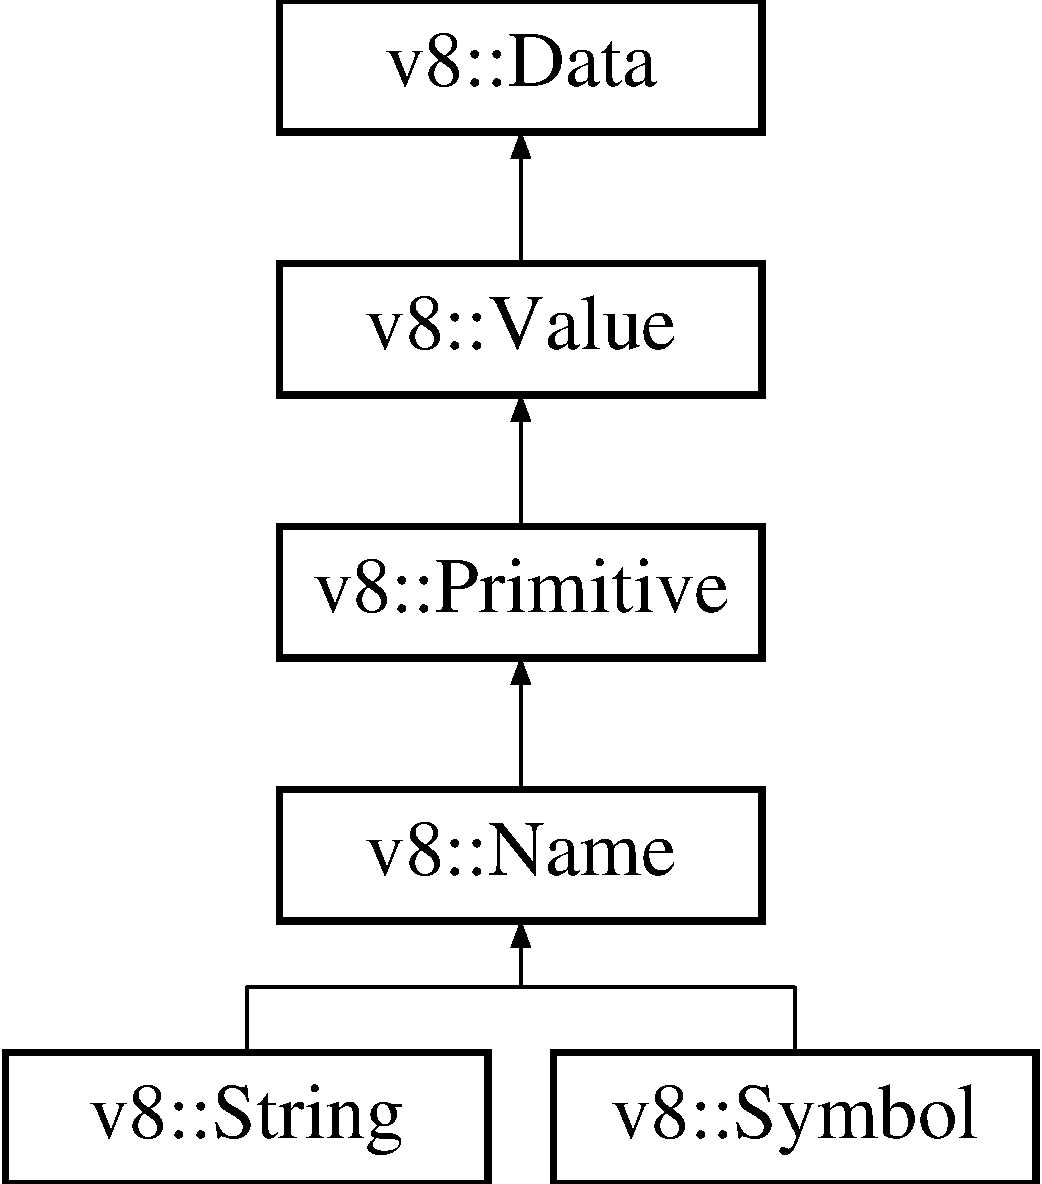
\includegraphics[height=5.000000cm]{classv8_1_1Name}
\end{center}
\end{figure}
\subsection*{Public Member Functions}
\begin{DoxyCompactItemize}
\item 
int \mbox{\hyperlink{classv8_1_1Name_aef60fce47685fad12914304f6bc52bf2}{Get\+Identity\+Hash}} ()
\end{DoxyCompactItemize}
\subsection*{Static Public Member Functions}
\begin{DoxyCompactItemize}
\item 
\mbox{\Hypertarget{classv8_1_1Name_a38bb2124c25f5089afd5fc1f9e87066f}\label{classv8_1_1Name_a38bb2124c25f5089afd5fc1f9e87066f}} 
static V8\+\_\+\+I\+N\+L\+I\+NE \mbox{\hyperlink{classv8_1_1Name}{Name}} $\ast$ {\bfseries Cast} (\mbox{\hyperlink{classv8_1_1Value}{Value}} $\ast$obj)
\end{DoxyCompactItemize}


\subsection{Detailed Description}
A superclass for symbols and strings. 

Definition at line 2497 of file v8.\+h.



\subsection{Member Function Documentation}
\mbox{\Hypertarget{classv8_1_1Name_aef60fce47685fad12914304f6bc52bf2}\label{classv8_1_1Name_aef60fce47685fad12914304f6bc52bf2}} 
\index{v8\+::\+Name@{v8\+::\+Name}!Get\+Identity\+Hash@{Get\+Identity\+Hash}}
\index{Get\+Identity\+Hash@{Get\+Identity\+Hash}!v8\+::\+Name@{v8\+::\+Name}}
\subsubsection{\texorpdfstring{Get\+Identity\+Hash()}{GetIdentityHash()}}
{\footnotesize\ttfamily int v8\+::\+Name\+::\+Get\+Identity\+Hash (\begin{DoxyParamCaption}{ }\end{DoxyParamCaption})}

Returns the identity hash for this object. The current implementation uses an inline property on the object to store the identity hash.

The return value will never be 0. Also, it is not guaranteed to be unique. 

The documentation for this class was generated from the following file\+:\begin{DoxyCompactItemize}
\item 
v8/include/v8.\+h\end{DoxyCompactItemize}

\hypertarget{structv8_1_1JitCodeEvent_1_1name__t}{}\section{v8\+:\+:Jit\+Code\+Event\+:\+:name\+\_\+t Struct Reference}
\label{structv8_1_1JitCodeEvent_1_1name__t}\index{v8\+::\+Jit\+Code\+Event\+::name\+\_\+t@{v8\+::\+Jit\+Code\+Event\+::name\+\_\+t}}
\subsection*{Data Fields}
\begin{DoxyCompactItemize}
\item 
\hypertarget{structv8_1_1JitCodeEvent_1_1name__t_a344732b4289a6a1fd21bb577ac9eff15}{}const char $\ast$ {\bfseries str}\label{structv8_1_1JitCodeEvent_1_1name__t_a344732b4289a6a1fd21bb577ac9eff15}

\item 
\hypertarget{structv8_1_1JitCodeEvent_1_1name__t_aa85ddd240f3b08c995caa8267ee8c586}{}size\+\_\+t {\bfseries len}\label{structv8_1_1JitCodeEvent_1_1name__t_aa85ddd240f3b08c995caa8267ee8c586}

\end{DoxyCompactItemize}


The documentation for this struct was generated from the following file\+:\begin{DoxyCompactItemize}
\item 
v8/include/v8.\+h\end{DoxyCompactItemize}

\hypertarget{structv8_1_1NamedPropertyHandlerConfiguration}{}\section{v8\+:\+:Named\+Property\+Handler\+Configuration Struct Reference}
\label{structv8_1_1NamedPropertyHandlerConfiguration}\index{v8\+::\+Named\+Property\+Handler\+Configuration@{v8\+::\+Named\+Property\+Handler\+Configuration}}
\subsection*{Public Member Functions}
\begin{DoxyCompactItemize}
\item 
\hyperlink{structv8_1_1NamedPropertyHandlerConfiguration_a7304ee88edae7f7342f3a03f7974202d}{Named\+Property\+Handler\+Configuration} (\hyperlink{namespacev8_a24b1801fa53a7c5a71366d8044927563}{Generic\+Named\+Property\+Getter\+Callback} getter=0, \hyperlink{namespacev8_af74716c6e95a269c6cd4314662fd0a7e}{Generic\+Named\+Property\+Setter\+Callback} setter=0, \hyperlink{namespacev8_add9f7ab11e4a9a2b9ad2c4536b0e1a64}{Generic\+Named\+Property\+Query\+Callback} query=0, \hyperlink{namespacev8_ad2aecc0406ea4bc02d5a4f84a433b273}{Generic\+Named\+Property\+Deleter\+Callback} deleter=0, \hyperlink{namespacev8_a20826eb7e52e84fa4f632534e8eddd04}{Generic\+Named\+Property\+Enumerator\+Callback} enumerator=0, \hyperlink{classv8_1_1Local}{Local}$<$ \hyperlink{classv8_1_1Value}{Value} $>$ data=\hyperlink{classv8_1_1Local}{Local}$<$ \hyperlink{classv8_1_1Value}{Value} $>$(), Property\+Handler\+Flags flags=Property\+Handler\+Flags\+::k\+None)
\end{DoxyCompactItemize}
\subsection*{Data Fields}
\begin{DoxyCompactItemize}
\item 
\hypertarget{structv8_1_1NamedPropertyHandlerConfiguration_a7e0f2f6be4b716330f78e08dafb43512}{}\hyperlink{namespacev8_a24b1801fa53a7c5a71366d8044927563}{Generic\+Named\+Property\+Getter\+Callback} {\bfseries getter}\label{structv8_1_1NamedPropertyHandlerConfiguration_a7e0f2f6be4b716330f78e08dafb43512}

\item 
\hypertarget{structv8_1_1NamedPropertyHandlerConfiguration_a03a2c13ff0e66f02c5944620c38dcf61}{}\hyperlink{namespacev8_af74716c6e95a269c6cd4314662fd0a7e}{Generic\+Named\+Property\+Setter\+Callback} {\bfseries setter}\label{structv8_1_1NamedPropertyHandlerConfiguration_a03a2c13ff0e66f02c5944620c38dcf61}

\item 
\hypertarget{structv8_1_1NamedPropertyHandlerConfiguration_af55d318e48d6f78b2103f3e603c86e34}{}\hyperlink{namespacev8_add9f7ab11e4a9a2b9ad2c4536b0e1a64}{Generic\+Named\+Property\+Query\+Callback} {\bfseries query}\label{structv8_1_1NamedPropertyHandlerConfiguration_af55d318e48d6f78b2103f3e603c86e34}

\item 
\hypertarget{structv8_1_1NamedPropertyHandlerConfiguration_ab6f53889af636ead0218b02d3eda38c6}{}\hyperlink{namespacev8_ad2aecc0406ea4bc02d5a4f84a433b273}{Generic\+Named\+Property\+Deleter\+Callback} {\bfseries deleter}\label{structv8_1_1NamedPropertyHandlerConfiguration_ab6f53889af636ead0218b02d3eda38c6}

\item 
\hypertarget{structv8_1_1NamedPropertyHandlerConfiguration_a9d24735d39fe1486a4235ccc48333be7}{}\hyperlink{namespacev8_a20826eb7e52e84fa4f632534e8eddd04}{Generic\+Named\+Property\+Enumerator\+Callback} {\bfseries enumerator}\label{structv8_1_1NamedPropertyHandlerConfiguration_a9d24735d39fe1486a4235ccc48333be7}

\item 
\hypertarget{structv8_1_1NamedPropertyHandlerConfiguration_a209f02c8b3202551bb8eef448d750f9d}{}\hyperlink{classv8_1_1Local}{Local}$<$ \hyperlink{classv8_1_1Value}{Value} $>$ {\bfseries data}\label{structv8_1_1NamedPropertyHandlerConfiguration_a209f02c8b3202551bb8eef448d750f9d}

\item 
\hypertarget{structv8_1_1NamedPropertyHandlerConfiguration_add28e99c72adf78b64e73f1de5aa74c7}{}Property\+Handler\+Flags {\bfseries flags}\label{structv8_1_1NamedPropertyHandlerConfiguration_add28e99c72adf78b64e73f1de5aa74c7}

\end{DoxyCompactItemize}


\subsection{Constructor \& Destructor Documentation}
\hypertarget{structv8_1_1NamedPropertyHandlerConfiguration_a7304ee88edae7f7342f3a03f7974202d}{}\index{v8\+::\+Named\+Property\+Handler\+Configuration@{v8\+::\+Named\+Property\+Handler\+Configuration}!Named\+Property\+Handler\+Configuration@{Named\+Property\+Handler\+Configuration}}
\index{Named\+Property\+Handler\+Configuration@{Named\+Property\+Handler\+Configuration}!v8\+::\+Named\+Property\+Handler\+Configuration@{v8\+::\+Named\+Property\+Handler\+Configuration}}
\subsubsection[{Named\+Property\+Handler\+Configuration}]{\setlength{\rightskip}{0pt plus 5cm}v8\+::\+Named\+Property\+Handler\+Configuration\+::\+Named\+Property\+Handler\+Configuration (
\begin{DoxyParamCaption}
\item[{{\bf Generic\+Named\+Property\+Getter\+Callback}}]{getter = {\ttfamily 0}, }
\item[{{\bf Generic\+Named\+Property\+Setter\+Callback}}]{setter = {\ttfamily 0}, }
\item[{{\bf Generic\+Named\+Property\+Query\+Callback}}]{query = {\ttfamily 0}, }
\item[{{\bf Generic\+Named\+Property\+Deleter\+Callback}}]{deleter = {\ttfamily 0}, }
\item[{{\bf Generic\+Named\+Property\+Enumerator\+Callback}}]{enumerator = {\ttfamily 0}, }
\item[{{\bf Local}$<$ {\bf Value} $>$}]{data = {\ttfamily {\bf Local}$<${\bf Value}$>$()}, }
\item[{Property\+Handler\+Flags}]{flags = {\ttfamily PropertyHandlerFlags\+:\+:kNone}}
\end{DoxyParamCaption}
)\hspace{0.3cm}{\ttfamily [inline]}}\label{structv8_1_1NamedPropertyHandlerConfiguration_a7304ee88edae7f7342f3a03f7974202d}

\begin{DoxyParams}{Parameters}
{\em getter} & Note\+: getter is required $\ast$ \\
\hline
\end{DoxyParams}


The documentation for this struct was generated from the following file\+:\begin{DoxyCompactItemize}
\item 
v8/include/v8.\+h\end{DoxyCompactItemize}

\hypertarget{classv8_1_1NativeWeakMap}{}\section{v8\+:\+:Native\+Weak\+Map Class Reference}
\label{classv8_1_1NativeWeakMap}\index{v8\+::\+Native\+Weak\+Map@{v8\+::\+Native\+Weak\+Map}}


{\ttfamily \#include $<$v8.\+h$>$}

Inheritance diagram for v8\+:\+:Native\+Weak\+Map\+:\begin{figure}[H]
\begin{center}
\leavevmode
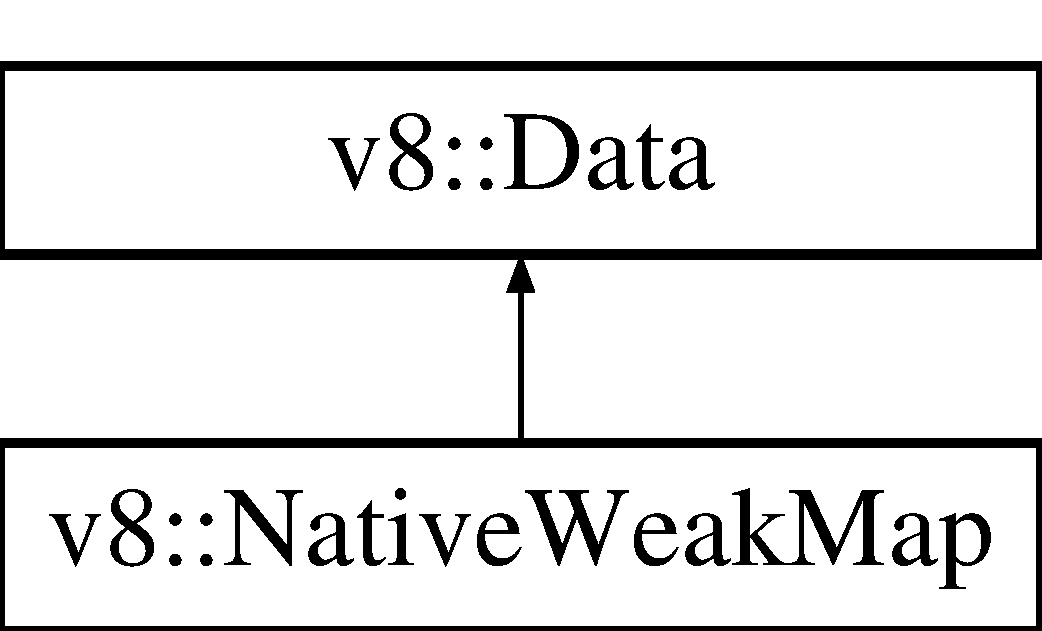
\includegraphics[height=2.000000cm]{classv8_1_1NativeWeakMap}
\end{center}
\end{figure}
\subsection*{Public Member Functions}
\begin{DoxyCompactItemize}
\item 
void {\bfseries Set} (\hyperlink{classv8_1_1Local}{Local}$<$ \hyperlink{classv8_1_1Value}{Value} $>$ key, \hyperlink{classv8_1_1Local}{Local}$<$ \hyperlink{classv8_1_1Value}{Value} $>$ value)\hypertarget{classv8_1_1NativeWeakMap_ade0e4ce74820a0fcf8b51fb1cea733a7}{}\label{classv8_1_1NativeWeakMap_ade0e4ce74820a0fcf8b51fb1cea733a7}

\item 
\hyperlink{classv8_1_1Local}{Local}$<$ \hyperlink{classv8_1_1Value}{Value} $>$ {\bfseries Get} (\hyperlink{classv8_1_1Local}{Local}$<$ \hyperlink{classv8_1_1Value}{Value} $>$ key)\hypertarget{classv8_1_1NativeWeakMap_a9350148caa6f09f7c228dda255317387}{}\label{classv8_1_1NativeWeakMap_a9350148caa6f09f7c228dda255317387}

\item 
bool {\bfseries Has} (\hyperlink{classv8_1_1Local}{Local}$<$ \hyperlink{classv8_1_1Value}{Value} $>$ key)\hypertarget{classv8_1_1NativeWeakMap_a9de62c6399280088c86bb57c3988e7cb}{}\label{classv8_1_1NativeWeakMap_a9de62c6399280088c86bb57c3988e7cb}

\item 
bool {\bfseries Delete} (\hyperlink{classv8_1_1Local}{Local}$<$ \hyperlink{classv8_1_1Value}{Value} $>$ key)\hypertarget{classv8_1_1NativeWeakMap_ae3c04eaa9e745732f7b2f16c6e75dead}{}\label{classv8_1_1NativeWeakMap_ae3c04eaa9e745732f7b2f16c6e75dead}

\end{DoxyCompactItemize}
\subsection*{Static Public Member Functions}
\begin{DoxyCompactItemize}
\item 
static \hyperlink{classv8_1_1Local}{Local}$<$ \hyperlink{classv8_1_1NativeWeakMap}{Native\+Weak\+Map} $>$ {\bfseries New} (\hyperlink{classv8_1_1Isolate}{Isolate} $\ast$isolate)\hypertarget{classv8_1_1NativeWeakMap_afeb513d14fbb8d4537e4a051c71fbf31}{}\label{classv8_1_1NativeWeakMap_afeb513d14fbb8d4537e4a051c71fbf31}

\end{DoxyCompactItemize}


\subsection{Detailed Description}
A map whose keys are referenced weakly. It is similar to Java\+Script Weak\+Map but can be created without entering a \hyperlink{classv8_1_1Context}{v8\+::\+Context} and hence shouldn\textquotesingle{}t escape to Java\+Script. 

The documentation for this class was generated from the following file\+:\begin{DoxyCompactItemize}
\item 
v8/include/v8.\+h\end{DoxyCompactItemize}

\hypertarget{classv8_1_1NonCopyablePersistentTraits}{}\section{v8\+:\+:Non\+Copyable\+Persistent\+Traits$<$ T $>$ Class Template Reference}
\label{classv8_1_1NonCopyablePersistentTraits}\index{v8\+::\+Non\+Copyable\+Persistent\+Traits$<$ T $>$@{v8\+::\+Non\+Copyable\+Persistent\+Traits$<$ T $>$}}


{\ttfamily \#include $<$v8.\+h$>$}

\subsection*{Public Types}
\begin{DoxyCompactItemize}
\item 
\mbox{\Hypertarget{classv8_1_1NonCopyablePersistentTraits_af26082b31726b82c0482a01daa2f3e54}\label{classv8_1_1NonCopyablePersistentTraits_af26082b31726b82c0482a01daa2f3e54}} 
typedef \mbox{\hyperlink{classv8_1_1Persistent}{Persistent}}$<$ T, \mbox{\hyperlink{classv8_1_1NonCopyablePersistentTraits}{Non\+Copyable\+Persistent\+Traits}}$<$ T $>$ $>$ {\bfseries Non\+Copyable\+Persistent}
\end{DoxyCompactItemize}
\subsection*{Static Public Member Functions}
\begin{DoxyCompactItemize}
\item 
\mbox{\Hypertarget{classv8_1_1NonCopyablePersistentTraits_a40b133b17a334c5c7674135e7dbcf850}\label{classv8_1_1NonCopyablePersistentTraits_a40b133b17a334c5c7674135e7dbcf850}} 
{\footnotesize template$<$class S , class M $>$ }\\static V8\+\_\+\+I\+N\+L\+I\+NE void {\bfseries Copy} (const \mbox{\hyperlink{classv8_1_1Persistent}{Persistent}}$<$ S, M $>$ \&source, \mbox{\hyperlink{classv8_1_1Persistent}{Non\+Copyable\+Persistent}} $\ast$dest)
\item 
\mbox{\Hypertarget{classv8_1_1NonCopyablePersistentTraits_a90e2c6958ba089f5fabbbc7c08f976c1}\label{classv8_1_1NonCopyablePersistentTraits_a90e2c6958ba089f5fabbbc7c08f976c1}} 
{\footnotesize template$<$class O $>$ }\\static V8\+\_\+\+I\+N\+L\+I\+NE void {\bfseries Uncompilable} ()
\end{DoxyCompactItemize}
\subsection*{Static Public Attributes}
\begin{DoxyCompactItemize}
\item 
\mbox{\Hypertarget{classv8_1_1NonCopyablePersistentTraits_a650880d85ff80634c30a195d20329681}\label{classv8_1_1NonCopyablePersistentTraits_a650880d85ff80634c30a195d20329681}} 
static const bool {\bfseries k\+Reset\+In\+Destructor} = false
\end{DoxyCompactItemize}


\subsection{Detailed Description}
\subsubsection*{template$<$class T$>$\newline
class v8\+::\+Non\+Copyable\+Persistent\+Traits$<$ T $>$}

Default traits for \mbox{\hyperlink{classv8_1_1Persistent}{Persistent}}. This class does not allow use of the copy constructor or assignment operator. At present k\+Reset\+In\+Destructor is not set, but that will change in a future version. 

The documentation for this class was generated from the following file\+:\begin{DoxyCompactItemize}
\item 
v8/include/v8.\+h\end{DoxyCompactItemize}

\hypertarget{classv8_1_1Number}{}\section{v8\+:\+:Number Class Reference}
\label{classv8_1_1Number}\index{v8\+::\+Number@{v8\+::\+Number}}


{\ttfamily \#include $<$v8.\+h$>$}

Inheritance diagram for v8\+:\+:Number\+:\begin{figure}[H]
\begin{center}
\leavevmode
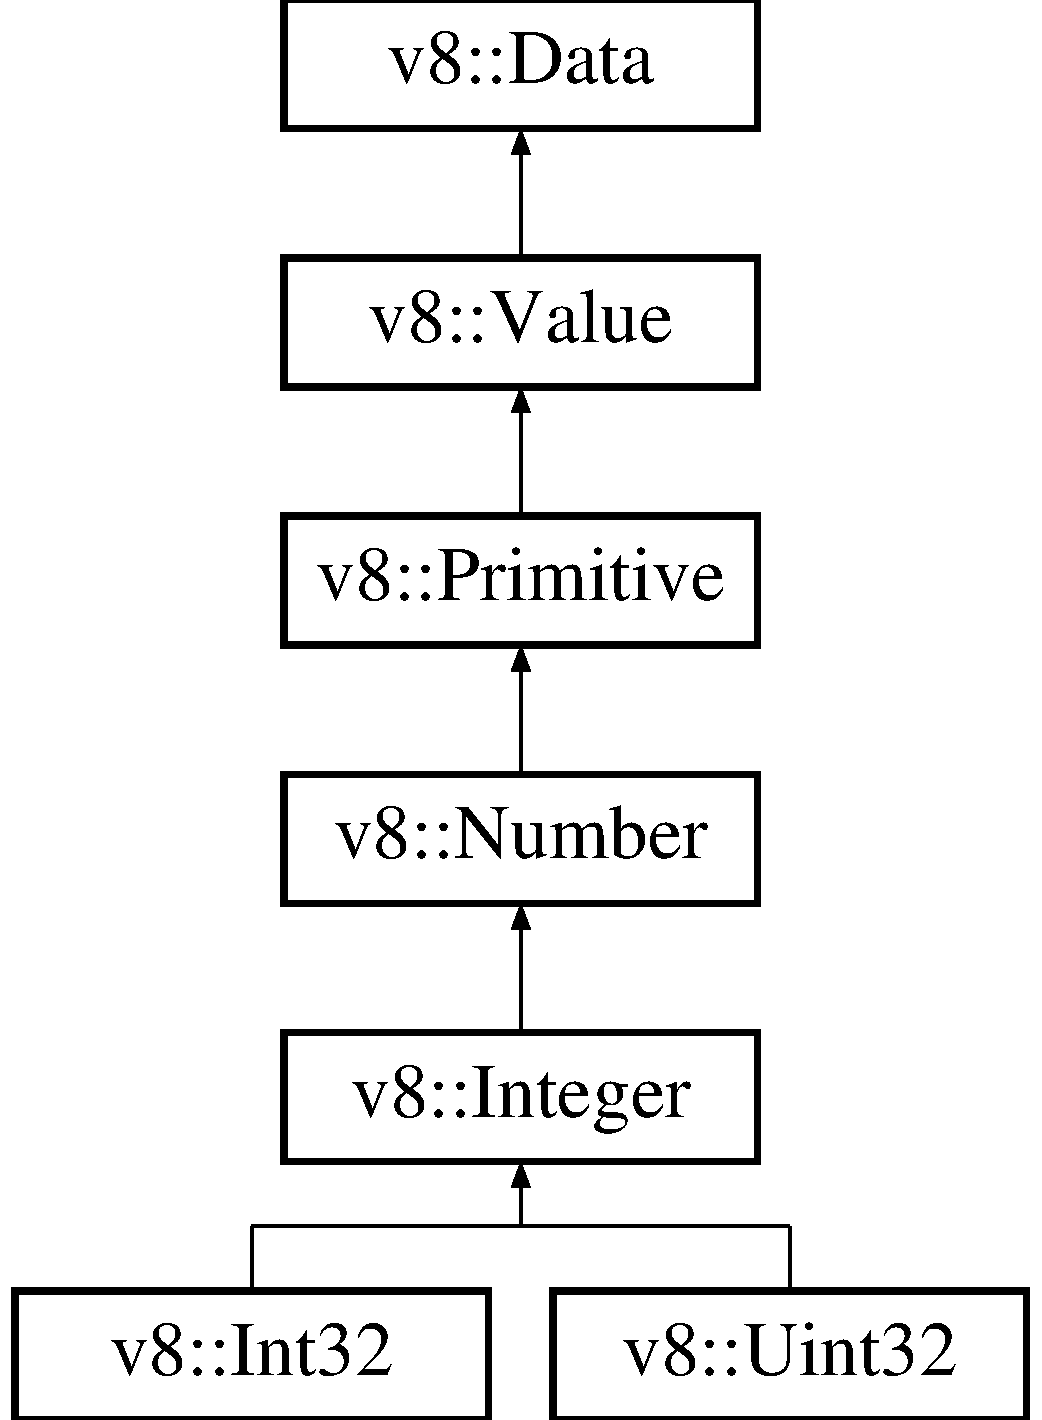
\includegraphics[height=6.000000cm]{classv8_1_1Number}
\end{center}
\end{figure}
\subsection*{Public Member Functions}
\begin{DoxyCompactItemize}
\item 
\mbox{\Hypertarget{classv8_1_1Number_aed515db835eefc10820d45c60775e950}\label{classv8_1_1Number_aed515db835eefc10820d45c60775e950}} 
double {\bfseries Value} () const
\end{DoxyCompactItemize}
\subsection*{Static Public Member Functions}
\begin{DoxyCompactItemize}
\item 
\mbox{\Hypertarget{classv8_1_1Number_a90ea55018560648ffaf8861372b41928}\label{classv8_1_1Number_a90ea55018560648ffaf8861372b41928}} 
static \mbox{\hyperlink{classv8_1_1Local}{Local}}$<$ \mbox{\hyperlink{classv8_1_1Number}{Number}} $>$ {\bfseries New} (Isolate $\ast$isolate, double value)
\item 
\mbox{\Hypertarget{classv8_1_1Number_a053d48e0003104308963a4a7e3881912}\label{classv8_1_1Number_a053d48e0003104308963a4a7e3881912}} 
static V8\+\_\+\+I\+N\+L\+I\+NE \mbox{\hyperlink{classv8_1_1Number}{Number}} $\ast$ {\bfseries Cast} (\mbox{\hyperlink{classv8_1_1Value}{v8\+::\+Value}} $\ast$obj)
\end{DoxyCompactItemize}


\subsection{Detailed Description}
A Java\+Script number value (E\+C\+M\+A-\/262, 4.\+3.\+20) 

Definition at line 3021 of file v8.\+h.



The documentation for this class was generated from the following file\+:\begin{DoxyCompactItemize}
\item 
v8/include/v8.\+h\end{DoxyCompactItemize}

\hypertarget{classv8_1_1NumberObject}{}\section{v8\+:\+:Number\+Object Class Reference}
\label{classv8_1_1NumberObject}\index{v8\+::\+Number\+Object@{v8\+::\+Number\+Object}}


{\ttfamily \#include $<$v8.\+h$>$}

Inheritance diagram for v8\+:\+:Number\+Object\+:\begin{figure}[H]
\begin{center}
\leavevmode
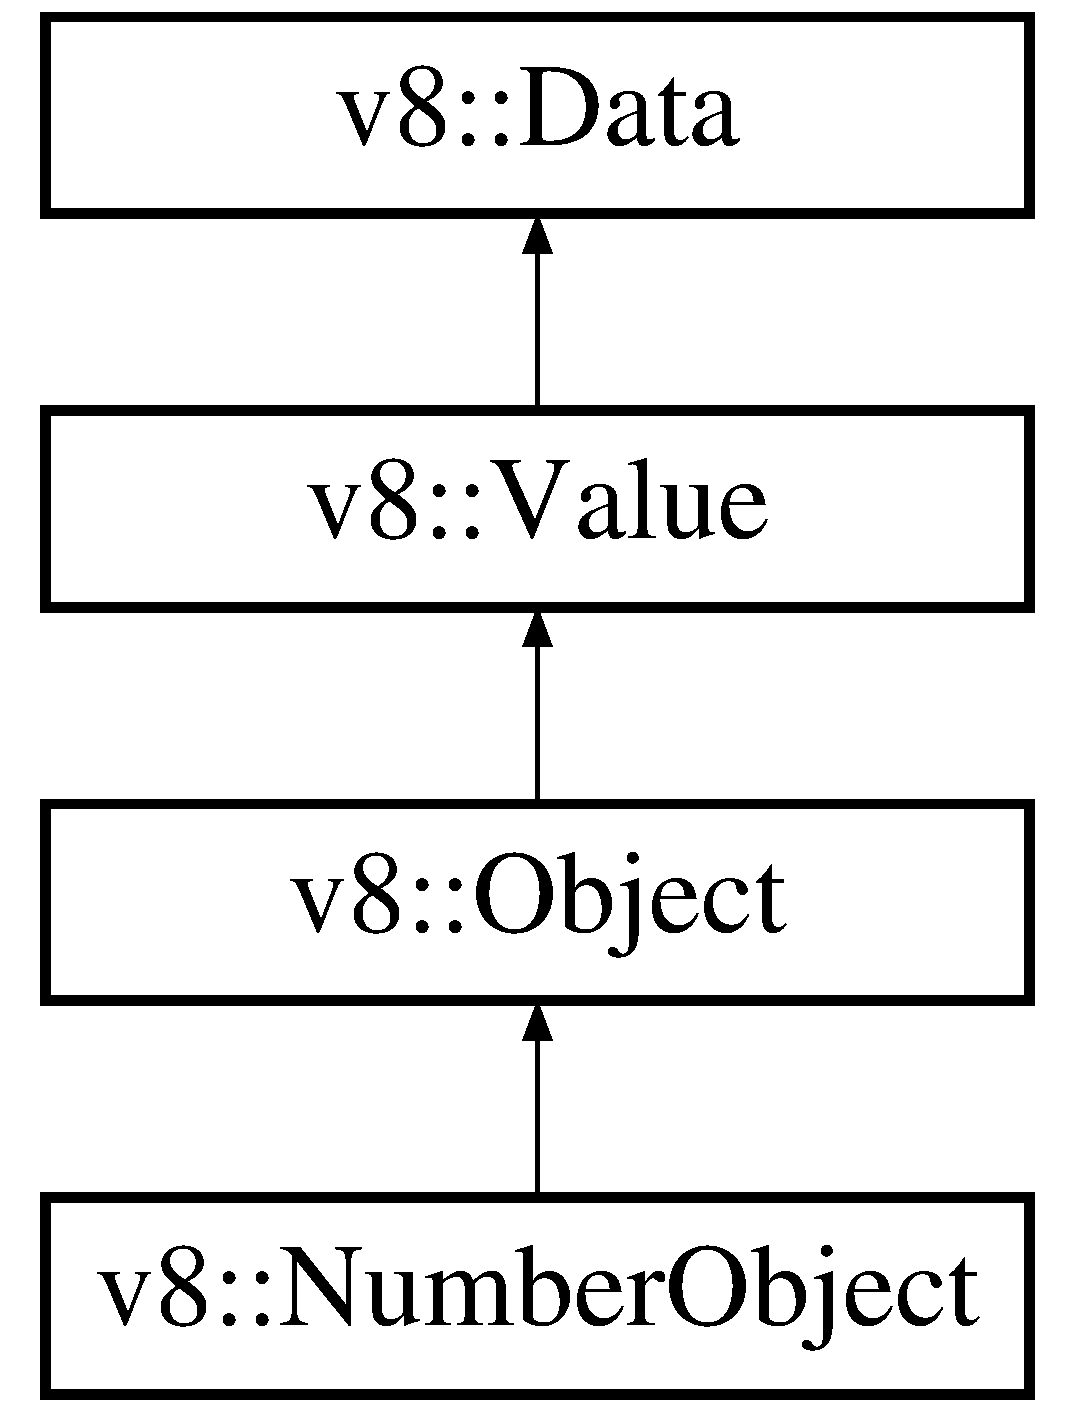
\includegraphics[height=4.000000cm]{classv8_1_1NumberObject}
\end{center}
\end{figure}
\subsection*{Public Member Functions}
\begin{DoxyCompactItemize}
\item 
double {\bfseries Value\+Of} () const \hypertarget{classv8_1_1NumberObject_a40c7211d55bc2de1b23f475d1906b5bf}{}\label{classv8_1_1NumberObject_a40c7211d55bc2de1b23f475d1906b5bf}

\end{DoxyCompactItemize}
\subsection*{Static Public Member Functions}
\begin{DoxyCompactItemize}
\item 
static \hyperlink{classv8_1_1Local}{Local}$<$ \hyperlink{classv8_1_1Value}{Value} $>$ {\bfseries New} (\hyperlink{classv8_1_1Isolate}{Isolate} $\ast$isolate, double value)\hypertarget{classv8_1_1NumberObject_ad6e3d9fe36d6389fe90f2645cab8a2d7}{}\label{classv8_1_1NumberObject_ad6e3d9fe36d6389fe90f2645cab8a2d7}

\item 
static V8\+\_\+\+I\+N\+L\+I\+NE \hyperlink{classv8_1_1NumberObject}{Number\+Object} $\ast$ {\bfseries Cast} (\hyperlink{classv8_1_1Value}{v8\+::\+Value} $\ast$obj)\hypertarget{classv8_1_1NumberObject_a0dad558fde0ec8e51ff53a3e34dbce7e}{}\label{classv8_1_1NumberObject_a0dad558fde0ec8e51ff53a3e34dbce7e}

\end{DoxyCompactItemize}


\subsection{Detailed Description}
A \hyperlink{classv8_1_1Number}{Number} object (E\+C\+M\+A-\/262, 4.\+3.\+21). 

The documentation for this class was generated from the following file\+:\begin{DoxyCompactItemize}
\item 
v8/include/v8.\+h\end{DoxyCompactItemize}

\hypertarget{classv8_1_1Object}{}\section{v8\+:\+:Object Class Reference}
\label{classv8_1_1Object}\index{v8\+::\+Object@{v8\+::\+Object}}


{\ttfamily \#include $<$v8.\+h$>$}

Inheritance diagram for v8\+:\+:Object\+:\begin{figure}[H]
\begin{center}
\leavevmode
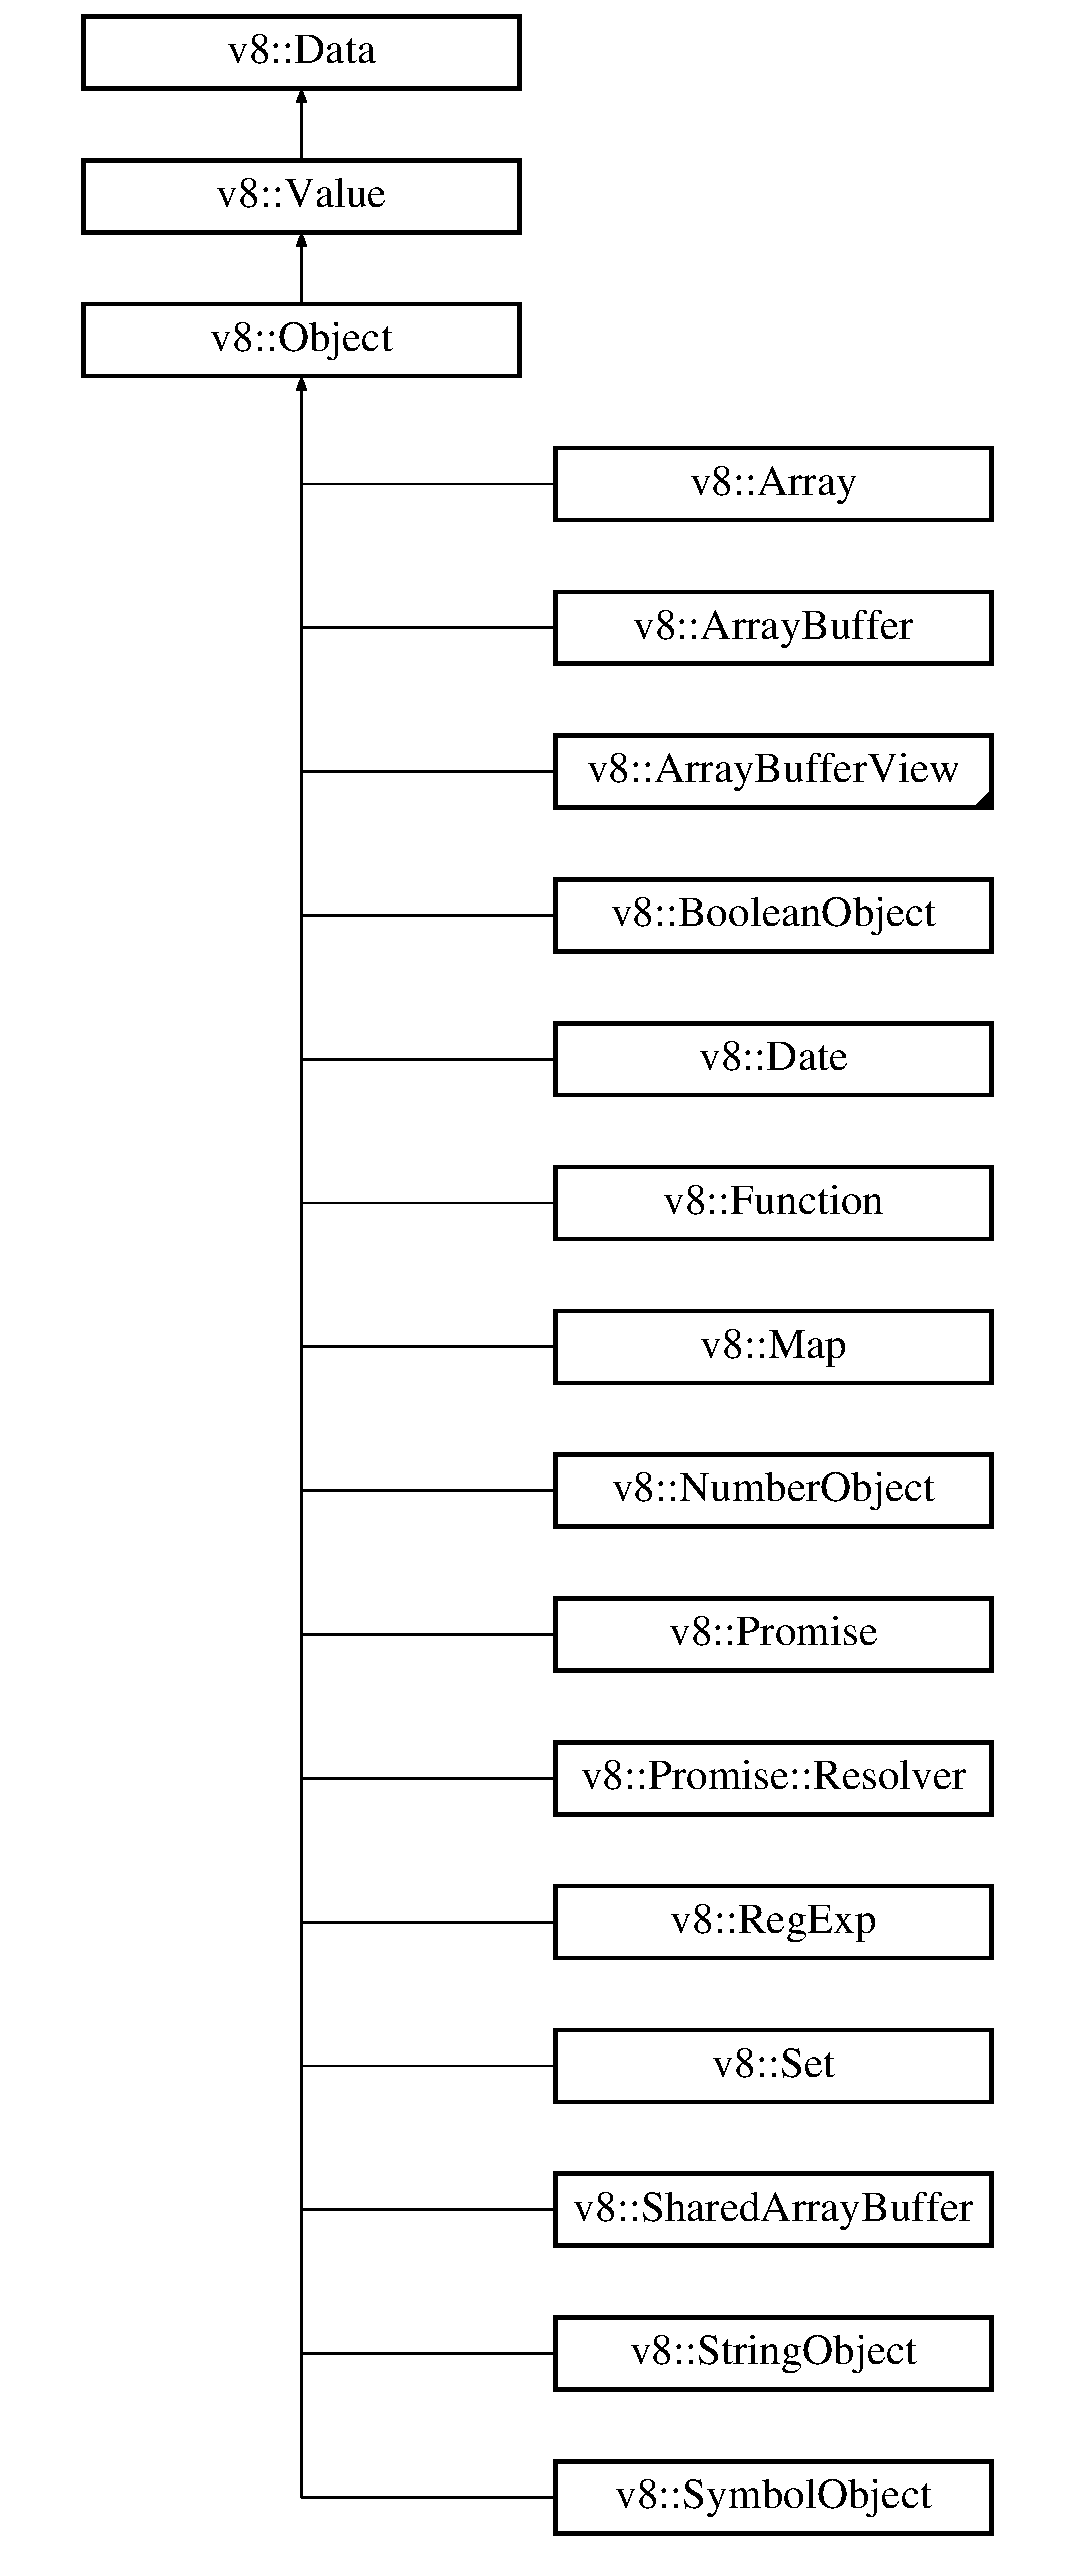
\includegraphics[height=12.000000cm]{classv8_1_1Object}
\end{center}
\end{figure}
\subsection*{Public Member Functions}
\begin{DoxyCompactItemize}
\item 
{\bfseries V8\+\_\+\+D\+E\+P\+R\+E\+C\+A\+T\+E\+\_\+\+S\+O\+ON} (\char`\"{}Use maybe version\char`\"{}, bool \hyperlink{classv8_1_1Set}{Set}(\hyperlink{classv8_1_1Local}{Local}$<$ \hyperlink{classv8_1_1Value}{Value} $>$ key, \hyperlink{classv8_1_1Local}{Local}$<$ \hyperlink{classv8_1_1Value}{Value} $>$ value))\hypertarget{classv8_1_1Object_a86333122230b703cabfb08d8a7d54a58}{}\label{classv8_1_1Object_a86333122230b703cabfb08d8a7d54a58}

\item 
V8\+\_\+\+W\+A\+R\+N\+\_\+\+U\+N\+U\+S\+E\+D\+\_\+\+R\+E\+S\+U\+LT \hyperlink{classv8_1_1Maybe}{Maybe}$<$ bool $>$ {\bfseries Set} (\hyperlink{classv8_1_1Local}{Local}$<$ \hyperlink{classv8_1_1Context}{Context} $>$ context, \hyperlink{classv8_1_1Local}{Local}$<$ \hyperlink{classv8_1_1Value}{Value} $>$ key, \hyperlink{classv8_1_1Local}{Local}$<$ \hyperlink{classv8_1_1Value}{Value} $>$ value)\hypertarget{classv8_1_1Object_ac5840fc655bea7b2b55a4b49338360ae}{}\label{classv8_1_1Object_ac5840fc655bea7b2b55a4b49338360ae}

\item 
{\bfseries V8\+\_\+\+D\+E\+P\+R\+E\+C\+A\+T\+E\+\_\+\+S\+O\+ON} (\char`\"{}Use maybe version\char`\"{}, bool \hyperlink{classv8_1_1Set}{Set}(uint32\+\_\+t index, \hyperlink{classv8_1_1Local}{Local}$<$ \hyperlink{classv8_1_1Value}{Value} $>$ value))\hypertarget{classv8_1_1Object_a0c2305335e71c88d245dd1aa0060a2de}{}\label{classv8_1_1Object_a0c2305335e71c88d245dd1aa0060a2de}

\item 
V8\+\_\+\+W\+A\+R\+N\+\_\+\+U\+N\+U\+S\+E\+D\+\_\+\+R\+E\+S\+U\+LT \hyperlink{classv8_1_1Maybe}{Maybe}$<$ bool $>$ {\bfseries Set} (\hyperlink{classv8_1_1Local}{Local}$<$ \hyperlink{classv8_1_1Context}{Context} $>$ context, uint32\+\_\+t index, \hyperlink{classv8_1_1Local}{Local}$<$ \hyperlink{classv8_1_1Value}{Value} $>$ value)\hypertarget{classv8_1_1Object_ace0cbcf5659a82106601d07b3e6fa2be}{}\label{classv8_1_1Object_ace0cbcf5659a82106601d07b3e6fa2be}

\item 
V8\+\_\+\+W\+A\+R\+N\+\_\+\+U\+N\+U\+S\+E\+D\+\_\+\+R\+E\+S\+U\+LT \hyperlink{classv8_1_1Maybe}{Maybe}$<$ bool $>$ {\bfseries Create\+Data\+Property} (\hyperlink{classv8_1_1Local}{Local}$<$ \hyperlink{classv8_1_1Context}{Context} $>$ context, \hyperlink{classv8_1_1Local}{Local}$<$ \hyperlink{classv8_1_1Name}{Name} $>$ key, \hyperlink{classv8_1_1Local}{Local}$<$ \hyperlink{classv8_1_1Value}{Value} $>$ value)\hypertarget{classv8_1_1Object_ae334696b1e57ea2b333c4da48dd37895}{}\label{classv8_1_1Object_ae334696b1e57ea2b333c4da48dd37895}

\item 
V8\+\_\+\+W\+A\+R\+N\+\_\+\+U\+N\+U\+S\+E\+D\+\_\+\+R\+E\+S\+U\+LT \hyperlink{classv8_1_1Maybe}{Maybe}$<$ bool $>$ {\bfseries Create\+Data\+Property} (\hyperlink{classv8_1_1Local}{Local}$<$ \hyperlink{classv8_1_1Context}{Context} $>$ context, uint32\+\_\+t index, \hyperlink{classv8_1_1Local}{Local}$<$ \hyperlink{classv8_1_1Value}{Value} $>$ value)\hypertarget{classv8_1_1Object_aec3a99813837c0bc6444c59f8e5ca22a}{}\label{classv8_1_1Object_aec3a99813837c0bc6444c59f8e5ca22a}

\item 
V8\+\_\+\+W\+A\+R\+N\+\_\+\+U\+N\+U\+S\+E\+D\+\_\+\+R\+E\+S\+U\+LT \hyperlink{classv8_1_1Maybe}{Maybe}$<$ bool $>$ {\bfseries Define\+Own\+Property} (\hyperlink{classv8_1_1Local}{Local}$<$ \hyperlink{classv8_1_1Context}{Context} $>$ context, \hyperlink{classv8_1_1Local}{Local}$<$ \hyperlink{classv8_1_1Name}{Name} $>$ key, \hyperlink{classv8_1_1Local}{Local}$<$ \hyperlink{classv8_1_1Value}{Value} $>$ value, Property\+Attribute attributes=None)\hypertarget{classv8_1_1Object_a65f44f92b7ee9d479ce6b3ebb9ac8d4b}{}\label{classv8_1_1Object_a65f44f92b7ee9d479ce6b3ebb9ac8d4b}

\item 
{\bfseries V8\+\_\+\+D\+E\+P\+R\+E\+C\+A\+T\+ED} (\char`\"{}Use Create\+Data\+Property / Define\+Own\+Property\char`\"{}, bool Force\+Set(\hyperlink{classv8_1_1Local}{Local}$<$ \hyperlink{classv8_1_1Value}{Value} $>$ key, \hyperlink{classv8_1_1Local}{Local}$<$ \hyperlink{classv8_1_1Value}{Value} $>$ value,                                                                                                               Property\+Attribute attribs=None))\hypertarget{classv8_1_1Object_a91905983e337c86a9c6a38766856371d}{}\label{classv8_1_1Object_a91905983e337c86a9c6a38766856371d}

\item 
{\bfseries V8\+\_\+\+D\+E\+P\+R\+E\+C\+A\+T\+E\+\_\+\+S\+O\+ON} (\char`\"{}Use Create\+Data\+Property / Define\+Own\+Property\char`\"{}, Maybe$<$ bool $>$ Force\+Set(\hyperlink{classv8_1_1Local}{Local}$<$ \hyperlink{classv8_1_1Context}{Context} $>$ context,                                                                                                                                                           \hyperlink{classv8_1_1Local}{Local}$<$ \hyperlink{classv8_1_1Value}{Value} $>$ key, \hyperlink{classv8_1_1Local}{Local}$<$ \hyperlink{classv8_1_1Value}{Value} $>$ value,                                                                                                                                                           Property\+Attribute attribs=None))\hypertarget{classv8_1_1Object_a9b907489b6138ba8bfbc071ee0b3cdd5}{}\label{classv8_1_1Object_a9b907489b6138ba8bfbc071ee0b3cdd5}

\item 
{\bfseries V8\+\_\+\+D\+E\+P\+R\+E\+C\+A\+T\+E\+\_\+\+S\+O\+ON} (\char`\"{}Use maybe version\char`\"{}, Local$<$ \hyperlink{classv8_1_1Value}{Value} $>$ Get(\hyperlink{classv8_1_1Local}{Local}$<$ \hyperlink{classv8_1_1Value}{Value} $>$ key))\hypertarget{classv8_1_1Object_a15c40cda73a1927bef406b85032d5564}{}\label{classv8_1_1Object_a15c40cda73a1927bef406b85032d5564}

\item 
V8\+\_\+\+W\+A\+R\+N\+\_\+\+U\+N\+U\+S\+E\+D\+\_\+\+R\+E\+S\+U\+LT \hyperlink{classv8_1_1MaybeLocal}{Maybe\+Local}$<$ \hyperlink{classv8_1_1Value}{Value} $>$ {\bfseries Get} (\hyperlink{classv8_1_1Local}{Local}$<$ \hyperlink{classv8_1_1Context}{Context} $>$ context, \hyperlink{classv8_1_1Local}{Local}$<$ \hyperlink{classv8_1_1Value}{Value} $>$ key)\hypertarget{classv8_1_1Object_a239c03bb250cd6bf583ca60f72e18918}{}\label{classv8_1_1Object_a239c03bb250cd6bf583ca60f72e18918}

\item 
{\bfseries V8\+\_\+\+D\+E\+P\+R\+E\+C\+A\+T\+E\+\_\+\+S\+O\+ON} (\char`\"{}Use maybe version\char`\"{}, Local$<$ \hyperlink{classv8_1_1Value}{Value} $>$ Get(uint32\+\_\+t index))\hypertarget{classv8_1_1Object_ac27f1b680e53d4c9c879aac3c7380202}{}\label{classv8_1_1Object_ac27f1b680e53d4c9c879aac3c7380202}

\item 
V8\+\_\+\+W\+A\+R\+N\+\_\+\+U\+N\+U\+S\+E\+D\+\_\+\+R\+E\+S\+U\+LT \hyperlink{classv8_1_1MaybeLocal}{Maybe\+Local}$<$ \hyperlink{classv8_1_1Value}{Value} $>$ {\bfseries Get} (\hyperlink{classv8_1_1Local}{Local}$<$ \hyperlink{classv8_1_1Context}{Context} $>$ context, uint32\+\_\+t index)\hypertarget{classv8_1_1Object_ac1fcfcfedaf66775c46b53cb1804b949}{}\label{classv8_1_1Object_ac1fcfcfedaf66775c46b53cb1804b949}

\item 
\hyperlink{classv8_1_1Object_aa45eb69321fa3eb1037b058b69ecfec1}{V8\+\_\+\+D\+E\+P\+R\+E\+C\+A\+T\+ED} (\char`\"{}Use maybe version\char`\"{}, Property\+Attribute Get\+Property\+Attributes(\hyperlink{classv8_1_1Local}{Local}$<$ \hyperlink{classv8_1_1Value}{Value} $>$ key))
\item 
V8\+\_\+\+W\+A\+R\+N\+\_\+\+U\+N\+U\+S\+E\+D\+\_\+\+R\+E\+S\+U\+LT \hyperlink{classv8_1_1Maybe}{Maybe}$<$ Property\+Attribute $>$ {\bfseries Get\+Property\+Attributes} (\hyperlink{classv8_1_1Local}{Local}$<$ \hyperlink{classv8_1_1Context}{Context} $>$ context, \hyperlink{classv8_1_1Local}{Local}$<$ \hyperlink{classv8_1_1Value}{Value} $>$ key)\hypertarget{classv8_1_1Object_ae5c97a596bcb634c50605a574358a9c6}{}\label{classv8_1_1Object_ae5c97a596bcb634c50605a574358a9c6}

\item 
\hyperlink{classv8_1_1Object_ad914d35a19347cd1afdeea4e215f4999}{V8\+\_\+\+D\+E\+P\+R\+E\+C\+A\+T\+ED} (\char`\"{}Use maybe version\char`\"{}, Local$<$ \hyperlink{classv8_1_1Value}{Value} $>$ Get\+Own\+Property\+Descriptor(\hyperlink{classv8_1_1Local}{Local}$<$ \hyperlink{classv8_1_1String}{String} $>$ key))
\item 
V8\+\_\+\+W\+A\+R\+N\+\_\+\+U\+N\+U\+S\+E\+D\+\_\+\+R\+E\+S\+U\+LT \hyperlink{classv8_1_1MaybeLocal}{Maybe\+Local}$<$ \hyperlink{classv8_1_1Value}{Value} $>$ {\bfseries Get\+Own\+Property\+Descriptor} (\hyperlink{classv8_1_1Local}{Local}$<$ \hyperlink{classv8_1_1Context}{Context} $>$ context, \hyperlink{classv8_1_1Local}{Local}$<$ \hyperlink{classv8_1_1String}{String} $>$ key)\hypertarget{classv8_1_1Object_a17fd31922f11c634183c59c0eb08cf65}{}\label{classv8_1_1Object_a17fd31922f11c634183c59c0eb08cf65}

\item 
{\bfseries V8\+\_\+\+D\+E\+P\+R\+E\+C\+A\+T\+E\+\_\+\+S\+O\+ON} (\char`\"{}Use maybe version\char`\"{}, bool Has(\hyperlink{classv8_1_1Local}{Local}$<$ \hyperlink{classv8_1_1Value}{Value} $>$ key))\hypertarget{classv8_1_1Object_adbaa619d9f0588470c1e88532949da65}{}\label{classv8_1_1Object_adbaa619d9f0588470c1e88532949da65}

\item 
V8\+\_\+\+W\+A\+R\+N\+\_\+\+U\+N\+U\+S\+E\+D\+\_\+\+R\+E\+S\+U\+LT \hyperlink{classv8_1_1Maybe}{Maybe}$<$ bool $>$ {\bfseries Has} (\hyperlink{classv8_1_1Local}{Local}$<$ \hyperlink{classv8_1_1Context}{Context} $>$ context, \hyperlink{classv8_1_1Local}{Local}$<$ \hyperlink{classv8_1_1Value}{Value} $>$ key)\hypertarget{classv8_1_1Object_a57d4819c2cc13715ed22dd23cdc84d7c}{}\label{classv8_1_1Object_a57d4819c2cc13715ed22dd23cdc84d7c}

\item 
{\bfseries V8\+\_\+\+D\+E\+P\+R\+E\+C\+A\+T\+E\+\_\+\+S\+O\+ON} (\char`\"{}Use maybe version\char`\"{}, bool Delete(\hyperlink{classv8_1_1Local}{Local}$<$ \hyperlink{classv8_1_1Value}{Value} $>$ key))\hypertarget{classv8_1_1Object_ad76afc75f558f317a80b4f4b83c5cd53}{}\label{classv8_1_1Object_ad76afc75f558f317a80b4f4b83c5cd53}

\item 
\hyperlink{classv8_1_1Maybe}{Maybe}$<$ bool $>$ {\bfseries Delete} (\hyperlink{classv8_1_1Local}{Local}$<$ \hyperlink{classv8_1_1Context}{Context} $>$ context, \hyperlink{classv8_1_1Local}{Local}$<$ \hyperlink{classv8_1_1Value}{Value} $>$ key)\hypertarget{classv8_1_1Object_ab0626985ff54cbeeccef5e50656e5481}{}\label{classv8_1_1Object_ab0626985ff54cbeeccef5e50656e5481}

\item 
{\bfseries V8\+\_\+\+D\+E\+P\+R\+E\+C\+A\+T\+ED} (\char`\"{}Use maybe version\char`\"{}, bool Has(uint32\+\_\+t index))\hypertarget{classv8_1_1Object_a3ce6e6be77b337272e954a715e2e78de}{}\label{classv8_1_1Object_a3ce6e6be77b337272e954a715e2e78de}

\item 
V8\+\_\+\+W\+A\+R\+N\+\_\+\+U\+N\+U\+S\+E\+D\+\_\+\+R\+E\+S\+U\+LT \hyperlink{classv8_1_1Maybe}{Maybe}$<$ bool $>$ {\bfseries Has} (\hyperlink{classv8_1_1Local}{Local}$<$ \hyperlink{classv8_1_1Context}{Context} $>$ context, uint32\+\_\+t index)\hypertarget{classv8_1_1Object_adfbff82d3a45a69415ae99013a654daa}{}\label{classv8_1_1Object_adfbff82d3a45a69415ae99013a654daa}

\item 
{\bfseries V8\+\_\+\+D\+E\+P\+R\+E\+C\+A\+T\+ED} (\char`\"{}Use maybe version\char`\"{}, bool Delete(uint32\+\_\+t index))\hypertarget{classv8_1_1Object_ac0f010485bb637ce7b69141c695febc6}{}\label{classv8_1_1Object_ac0f010485bb637ce7b69141c695febc6}

\item 
\hyperlink{classv8_1_1Maybe}{Maybe}$<$ bool $>$ {\bfseries Delete} (\hyperlink{classv8_1_1Local}{Local}$<$ \hyperlink{classv8_1_1Context}{Context} $>$ context, uint32\+\_\+t index)\hypertarget{classv8_1_1Object_aabd005ef33ff69c15562d5296f4982d0}{}\label{classv8_1_1Object_aabd005ef33ff69c15562d5296f4982d0}

\item 
{\bfseries V8\+\_\+\+D\+E\+P\+R\+E\+C\+A\+T\+ED} (\char`\"{}Use maybe version\char`\"{}, bool Set\+Accessor(\hyperlink{classv8_1_1Local}{Local}$<$ \hyperlink{classv8_1_1String}{String} $>$ name,                                                                                                                           \hyperlink{namespacev8_a722613c87061708a4f1aa050d095f868}{Accessor\+Getter\+Callback} getter,                                                                                                                           Accessor\+Setter\+Callback setter=0,                                                                                                                           \hyperlink{classv8_1_1Local}{Local}$<$ \hyperlink{classv8_1_1Value}{Value} $>$ data=\hyperlink{classv8_1_1Local}{Local}$<$ \hyperlink{classv8_1_1Value}{Value} $>$(),                                                                                                                           \hyperlink{namespacev8_a31d8355cb043d7d2dda3f4a52760b64e}{Access\+Control} settings=D\+E\+F\+A\+U\+LT,                                                                                                                           Property\+Attribute attribute=None))\hypertarget{classv8_1_1Object_ad971da1abd6640388d75e8dbe06ae213}{}\label{classv8_1_1Object_ad971da1abd6640388d75e8dbe06ae213}

\item 
{\bfseries V8\+\_\+\+D\+E\+P\+R\+E\+C\+A\+T\+ED} (\char`\"{}Use maybe version\char`\"{}, bool Set\+Accessor(\hyperlink{classv8_1_1Local}{Local}$<$ \hyperlink{classv8_1_1Name}{Name} $>$ name,                                                                                                                           Accessor\+Name\+Getter\+Callback getter,                                                                                                                           Accessor\+Name\+Setter\+Callback setter=0,                                                                                                                           \hyperlink{classv8_1_1Local}{Local}$<$ \hyperlink{classv8_1_1Value}{Value} $>$ data=\hyperlink{classv8_1_1Local}{Local}$<$ \hyperlink{classv8_1_1Value}{Value} $>$(),                                                                                                                           \hyperlink{namespacev8_a31d8355cb043d7d2dda3f4a52760b64e}{Access\+Control} settings=D\+E\+F\+A\+U\+LT,                                                                                                                           Property\+Attribute attribute=None))\hypertarget{classv8_1_1Object_ad1128988b65b95ae5a4dab8c5fcf38b5}{}\label{classv8_1_1Object_ad1128988b65b95ae5a4dab8c5fcf38b5}

\item 
\hyperlink{classv8_1_1Maybe}{Maybe}$<$ bool $>$ {\bfseries Set\+Accessor} (\hyperlink{classv8_1_1Local}{Local}$<$ \hyperlink{classv8_1_1Context}{Context} $>$ context, \hyperlink{classv8_1_1Local}{Local}$<$ \hyperlink{classv8_1_1Name}{Name} $>$ name, Accessor\+Name\+Getter\+Callback getter, Accessor\+Name\+Setter\+Callback setter=0, \hyperlink{classv8_1_1MaybeLocal}{Maybe\+Local}$<$ \hyperlink{classv8_1_1Value}{Value} $>$ data=\hyperlink{classv8_1_1MaybeLocal}{Maybe\+Local}$<$ \hyperlink{classv8_1_1Value}{Value} $>$(), \hyperlink{namespacev8_a31d8355cb043d7d2dda3f4a52760b64e}{Access\+Control} settings=D\+E\+F\+A\+U\+LT, Property\+Attribute attribute=None)\hypertarget{classv8_1_1Object_a6ab0b45aa38debc2cc9877ae3b232e55}{}\label{classv8_1_1Object_a6ab0b45aa38debc2cc9877ae3b232e55}

\item 
void {\bfseries Set\+Accessor\+Property} (\hyperlink{classv8_1_1Local}{Local}$<$ \hyperlink{classv8_1_1Name}{Name} $>$ name, \hyperlink{classv8_1_1Local}{Local}$<$ \hyperlink{classv8_1_1Function}{Function} $>$ getter, \hyperlink{classv8_1_1Local}{Local}$<$ \hyperlink{classv8_1_1Function}{Function} $>$ setter=\hyperlink{classv8_1_1Local}{Local}$<$ \hyperlink{classv8_1_1Function}{Function} $>$(), Property\+Attribute attribute=None, \hyperlink{namespacev8_a31d8355cb043d7d2dda3f4a52760b64e}{Access\+Control} settings=D\+E\+F\+A\+U\+LT)\hypertarget{classv8_1_1Object_a284911d760fc853d81adf98c242bc453}{}\label{classv8_1_1Object_a284911d760fc853d81adf98c242bc453}

\item 
\hyperlink{classv8_1_1Maybe}{Maybe}$<$ bool $>$ \hyperlink{classv8_1_1Object_aad699867935fd2142ec97afa6e39a7f0}{Has\+Private} (\hyperlink{classv8_1_1Local}{Local}$<$ \hyperlink{classv8_1_1Context}{Context} $>$ context, \hyperlink{classv8_1_1Local}{Local}$<$ \hyperlink{classv8_1_1Private}{Private} $>$ key)
\item 
\hyperlink{classv8_1_1Maybe}{Maybe}$<$ bool $>$ {\bfseries Set\+Private} (\hyperlink{classv8_1_1Local}{Local}$<$ \hyperlink{classv8_1_1Context}{Context} $>$ context, \hyperlink{classv8_1_1Local}{Local}$<$ \hyperlink{classv8_1_1Private}{Private} $>$ key, \hyperlink{classv8_1_1Local}{Local}$<$ \hyperlink{classv8_1_1Value}{Value} $>$ value)\hypertarget{classv8_1_1Object_a6ebc49302a65e706c52eeca31ba83283}{}\label{classv8_1_1Object_a6ebc49302a65e706c52eeca31ba83283}

\item 
\hyperlink{classv8_1_1Maybe}{Maybe}$<$ bool $>$ {\bfseries Delete\+Private} (\hyperlink{classv8_1_1Local}{Local}$<$ \hyperlink{classv8_1_1Context}{Context} $>$ context, \hyperlink{classv8_1_1Local}{Local}$<$ \hyperlink{classv8_1_1Private}{Private} $>$ key)\hypertarget{classv8_1_1Object_ad78ba140348f92581361329aab917382}{}\label{classv8_1_1Object_ad78ba140348f92581361329aab917382}

\item 
\hyperlink{classv8_1_1MaybeLocal}{Maybe\+Local}$<$ \hyperlink{classv8_1_1Value}{Value} $>$ {\bfseries Get\+Private} (\hyperlink{classv8_1_1Local}{Local}$<$ \hyperlink{classv8_1_1Context}{Context} $>$ context, \hyperlink{classv8_1_1Local}{Local}$<$ \hyperlink{classv8_1_1Private}{Private} $>$ key)\hypertarget{classv8_1_1Object_a6b2e55f1bf6b057c5cd9f2fc0e609c86}{}\label{classv8_1_1Object_a6b2e55f1bf6b057c5cd9f2fc0e609c86}

\item 
\hyperlink{classv8_1_1Object_a3f735ad2eab826ddc5eba467ce624acb}{V8\+\_\+\+D\+E\+P\+R\+E\+C\+A\+T\+E\+\_\+\+S\+O\+ON} (\char`\"{}Use maybe version\char`\"{}, Local$<$ \hyperlink{classv8_1_1Array}{Array} $>$ Get\+Property\+Names())
\item 
V8\+\_\+\+W\+A\+R\+N\+\_\+\+U\+N\+U\+S\+E\+D\+\_\+\+R\+E\+S\+U\+LT \hyperlink{classv8_1_1MaybeLocal}{Maybe\+Local}$<$ \hyperlink{classv8_1_1Array}{Array} $>$ {\bfseries Get\+Property\+Names} (\hyperlink{classv8_1_1Local}{Local}$<$ \hyperlink{classv8_1_1Context}{Context} $>$ context)\hypertarget{classv8_1_1Object_a771be1943535959085da5c384f8e6405}{}\label{classv8_1_1Object_a771be1943535959085da5c384f8e6405}

\item 
\hyperlink{classv8_1_1Object_aa72e9d0d22d1d4a4c4b63827a5469d40}{V8\+\_\+\+D\+E\+P\+R\+E\+C\+A\+T\+E\+\_\+\+S\+O\+ON} (\char`\"{}Use maybe version\char`\"{}, Local$<$ \hyperlink{classv8_1_1Array}{Array} $>$ Get\+Own\+Property\+Names())
\item 
V8\+\_\+\+W\+A\+R\+N\+\_\+\+U\+N\+U\+S\+E\+D\+\_\+\+R\+E\+S\+U\+LT \hyperlink{classv8_1_1MaybeLocal}{Maybe\+Local}$<$ \hyperlink{classv8_1_1Array}{Array} $>$ {\bfseries Get\+Own\+Property\+Names} (\hyperlink{classv8_1_1Local}{Local}$<$ \hyperlink{classv8_1_1Context}{Context} $>$ context)\hypertarget{classv8_1_1Object_ab4f1fc692a02c11d749a7d5120e67026}{}\label{classv8_1_1Object_ab4f1fc692a02c11d749a7d5120e67026}

\item 
\hyperlink{classv8_1_1Local}{Local}$<$ \hyperlink{classv8_1_1Value}{Value} $>$ \hyperlink{classv8_1_1Object_ae8d3fed7d6dbd667c29cabb3039fe7af}{Get\+Prototype} ()
\item 
\hyperlink{classv8_1_1Object_a4ce54e137e22eddbe2857a15a20219b2}{V8\+\_\+\+D\+E\+P\+R\+E\+C\+A\+T\+ED} (\char`\"{}Use maybe version\char`\"{}, bool Set\+Prototype(\hyperlink{classv8_1_1Local}{Local}$<$ \hyperlink{classv8_1_1Value}{Value} $>$ prototype))
\item 
V8\+\_\+\+W\+A\+R\+N\+\_\+\+U\+N\+U\+S\+E\+D\+\_\+\+R\+E\+S\+U\+LT \hyperlink{classv8_1_1Maybe}{Maybe}$<$ bool $>$ {\bfseries Set\+Prototype} (\hyperlink{classv8_1_1Local}{Local}$<$ \hyperlink{classv8_1_1Context}{Context} $>$ context, \hyperlink{classv8_1_1Local}{Local}$<$ \hyperlink{classv8_1_1Value}{Value} $>$ prototype)\hypertarget{classv8_1_1Object_a1f1fc25d2a440ad2a8b7d94db04f88fb}{}\label{classv8_1_1Object_a1f1fc25d2a440ad2a8b7d94db04f88fb}

\item 
\hyperlink{classv8_1_1Local}{Local}$<$ \hyperlink{classv8_1_1Object}{Object} $>$ \hyperlink{classv8_1_1Object_ae2ad9fee9db6e0e5da56973ebb8ea2bc}{Find\+Instance\+In\+Prototype\+Chain} (\hyperlink{classv8_1_1Local}{Local}$<$ \hyperlink{classv8_1_1FunctionTemplate}{Function\+Template} $>$ tmpl)
\item 
\hyperlink{classv8_1_1Object_a06bb9aab716e466b8fa0e0c3fbb8f5d7}{V8\+\_\+\+D\+E\+P\+R\+E\+C\+A\+T\+ED} (\char`\"{}Use maybe version\char`\"{}, Local$<$ \hyperlink{classv8_1_1String}{String} $>$ Object\+Proto\+To\+String())
\item 
V8\+\_\+\+W\+A\+R\+N\+\_\+\+U\+N\+U\+S\+E\+D\+\_\+\+R\+E\+S\+U\+LT \hyperlink{classv8_1_1MaybeLocal}{Maybe\+Local}$<$ \hyperlink{classv8_1_1String}{String} $>$ {\bfseries Object\+Proto\+To\+String} (\hyperlink{classv8_1_1Local}{Local}$<$ \hyperlink{classv8_1_1Context}{Context} $>$ context)\hypertarget{classv8_1_1Object_a7a65552d78eff4a1b9755f99167f4255}{}\label{classv8_1_1Object_a7a65552d78eff4a1b9755f99167f4255}

\item 
\hyperlink{classv8_1_1Local}{Local}$<$ \hyperlink{classv8_1_1String}{String} $>$ \hyperlink{classv8_1_1Object_a7bbe987794658f20a3ec1b68326305e6}{Get\+Constructor\+Name} ()
\item 
\hyperlink{classv8_1_1Maybe}{Maybe}$<$ bool $>$ \hyperlink{classv8_1_1Object_ac45163422a18bb7481cc78fcacecb301}{Set\+Integrity\+Level} (\hyperlink{classv8_1_1Local}{Local}$<$ \hyperlink{classv8_1_1Context}{Context} $>$ context, \hyperlink{namespacev8_a02642d03ff1eecc2fd358626499c2e30}{Integrity\+Level} level)
\item 
int \hyperlink{classv8_1_1Object_aaec28576353eebe6fee113bce2718ecc}{Internal\+Field\+Count} ()
\item 
V8\+\_\+\+I\+N\+L\+I\+NE \hyperlink{classv8_1_1Local}{Local}$<$ \hyperlink{classv8_1_1Value}{Value} $>$ \hyperlink{classv8_1_1Object_aa3324fdf652d8ac3b2f27faa0559231d}{Get\+Internal\+Field} (int index)
\item 
void \hyperlink{classv8_1_1Object_aebf949a0592cebc144bb2f96bfb7ec72}{Set\+Internal\+Field} (int index, \hyperlink{classv8_1_1Local}{Local}$<$ \hyperlink{classv8_1_1Value}{Value} $>$ value)
\item 
V8\+\_\+\+I\+N\+L\+I\+NE void $\ast$ \hyperlink{classv8_1_1Object_a435f68bb7ef0f64dd522c5c910682448}{Get\+Aligned\+Pointer\+From\+Internal\+Field} (int index)
\item 
void \hyperlink{classv8_1_1Object_a0ccba69581f0b5e4e672bab90f26879b}{Set\+Aligned\+Pointer\+In\+Internal\+Field} (int index, void $\ast$value)
\item 
{\bfseries V8\+\_\+\+D\+E\+P\+R\+E\+C\+A\+T\+ED} (\char`\"{}Use maybe version\char`\"{}, bool Has\+Own\+Property(\hyperlink{classv8_1_1Local}{Local}$<$ \hyperlink{classv8_1_1String}{String} $>$ key))\hypertarget{classv8_1_1Object_a332143937efdc58dac2d877ebeb5f8ef}{}\label{classv8_1_1Object_a332143937efdc58dac2d877ebeb5f8ef}

\item 
V8\+\_\+\+W\+A\+R\+N\+\_\+\+U\+N\+U\+S\+E\+D\+\_\+\+R\+E\+S\+U\+LT \hyperlink{classv8_1_1Maybe}{Maybe}$<$ bool $>$ {\bfseries Has\+Own\+Property} (\hyperlink{classv8_1_1Local}{Local}$<$ \hyperlink{classv8_1_1Context}{Context} $>$ context, \hyperlink{classv8_1_1Local}{Local}$<$ \hyperlink{classv8_1_1Name}{Name} $>$ key)\hypertarget{classv8_1_1Object_acdd3921e95d5bb1a27cea489792607ff}{}\label{classv8_1_1Object_acdd3921e95d5bb1a27cea489792607ff}

\item 
{\bfseries V8\+\_\+\+D\+E\+P\+R\+E\+C\+A\+T\+E\+\_\+\+S\+O\+ON} (\char`\"{}Use maybe version\char`\"{}, bool Has\+Real\+Named\+Property(\hyperlink{classv8_1_1Local}{Local}$<$ \hyperlink{classv8_1_1String}{String} $>$ key))\hypertarget{classv8_1_1Object_abf24b52a108c801a74718e1a1e64ba5b}{}\label{classv8_1_1Object_abf24b52a108c801a74718e1a1e64ba5b}

\item 
V8\+\_\+\+W\+A\+R\+N\+\_\+\+U\+N\+U\+S\+E\+D\+\_\+\+R\+E\+S\+U\+LT \hyperlink{classv8_1_1Maybe}{Maybe}$<$ bool $>$ {\bfseries Has\+Real\+Named\+Property} (\hyperlink{classv8_1_1Local}{Local}$<$ \hyperlink{classv8_1_1Context}{Context} $>$ context, \hyperlink{classv8_1_1Local}{Local}$<$ \hyperlink{classv8_1_1Name}{Name} $>$ key)\hypertarget{classv8_1_1Object_ad830b937c7586fe2086b288ea79935c4}{}\label{classv8_1_1Object_ad830b937c7586fe2086b288ea79935c4}

\item 
{\bfseries V8\+\_\+\+D\+E\+P\+R\+E\+C\+A\+T\+E\+\_\+\+S\+O\+ON} (\char`\"{}Use maybe version\char`\"{}, bool Has\+Real\+Indexed\+Property(uint32\+\_\+t index))\hypertarget{classv8_1_1Object_abd04e5cb82426a70ebea6afec8687c9e}{}\label{classv8_1_1Object_abd04e5cb82426a70ebea6afec8687c9e}

\item 
V8\+\_\+\+W\+A\+R\+N\+\_\+\+U\+N\+U\+S\+E\+D\+\_\+\+R\+E\+S\+U\+LT \hyperlink{classv8_1_1Maybe}{Maybe}$<$ bool $>$ {\bfseries Has\+Real\+Indexed\+Property} (\hyperlink{classv8_1_1Local}{Local}$<$ \hyperlink{classv8_1_1Context}{Context} $>$ context, uint32\+\_\+t index)\hypertarget{classv8_1_1Object_a46de2f348f4caafca287328ce385ab56}{}\label{classv8_1_1Object_a46de2f348f4caafca287328ce385ab56}

\item 
{\bfseries V8\+\_\+\+D\+E\+P\+R\+E\+C\+A\+T\+E\+\_\+\+S\+O\+ON} (\char`\"{}Use maybe version\char`\"{}, bool Has\+Real\+Named\+Callback\+Property(\hyperlink{classv8_1_1Local}{Local}$<$ \hyperlink{classv8_1_1String}{String} $>$ key))\hypertarget{classv8_1_1Object_ae1ffb11a0fa7549652d0530c0c4c4ca6}{}\label{classv8_1_1Object_ae1ffb11a0fa7549652d0530c0c4c4ca6}

\item 
V8\+\_\+\+W\+A\+R\+N\+\_\+\+U\+N\+U\+S\+E\+D\+\_\+\+R\+E\+S\+U\+LT \hyperlink{classv8_1_1Maybe}{Maybe}$<$ bool $>$ {\bfseries Has\+Real\+Named\+Callback\+Property} (\hyperlink{classv8_1_1Local}{Local}$<$ \hyperlink{classv8_1_1Context}{Context} $>$ context, \hyperlink{classv8_1_1Local}{Local}$<$ \hyperlink{classv8_1_1Name}{Name} $>$ key)\hypertarget{classv8_1_1Object_a62bde6bea1ce32b30b2152f33a105b14}{}\label{classv8_1_1Object_a62bde6bea1ce32b30b2152f33a105b14}

\item 
\hyperlink{classv8_1_1Object_a00982b58e0c86fcb37f5d74c8a33d1b8}{V8\+\_\+\+D\+E\+P\+R\+E\+C\+A\+T\+ED} (\char`\"{}Use maybe version\char`\"{}, Local$<$ \hyperlink{classv8_1_1Value}{Value} $>$ Get\+Real\+Named\+Property\+In\+Prototype\+Chain(\hyperlink{classv8_1_1Local}{Local}$<$ \hyperlink{classv8_1_1String}{String} $>$ key))
\item 
V8\+\_\+\+W\+A\+R\+N\+\_\+\+U\+N\+U\+S\+E\+D\+\_\+\+R\+E\+S\+U\+LT \hyperlink{classv8_1_1MaybeLocal}{Maybe\+Local}$<$ \hyperlink{classv8_1_1Value}{Value} $>$ {\bfseries Get\+Real\+Named\+Property\+In\+Prototype\+Chain} (\hyperlink{classv8_1_1Local}{Local}$<$ \hyperlink{classv8_1_1Context}{Context} $>$ context, \hyperlink{classv8_1_1Local}{Local}$<$ \hyperlink{classv8_1_1Name}{Name} $>$ key)\hypertarget{classv8_1_1Object_afe68d490fc41783e30126ca547b7fc90}{}\label{classv8_1_1Object_afe68d490fc41783e30126ca547b7fc90}

\item 
\hyperlink{classv8_1_1Object_ad227cb56752461c88badb0924132cfbc}{V8\+\_\+\+D\+E\+P\+R\+E\+C\+A\+T\+ED} (\char`\"{}Use maybe version\char`\"{}, Maybe$<$ Property\+Attribute $>$ Get\+Real\+Named\+Property\+Attributes\+In\+Prototype\+Chain(                               \hyperlink{classv8_1_1Local}{Local}$<$ \hyperlink{classv8_1_1String}{String} $>$ key))
\item 
V8\+\_\+\+W\+A\+R\+N\+\_\+\+U\+N\+U\+S\+E\+D\+\_\+\+R\+E\+S\+U\+LT \hyperlink{classv8_1_1Maybe}{Maybe}$<$ Property\+Attribute $>$ {\bfseries Get\+Real\+Named\+Property\+Attributes\+In\+Prototype\+Chain} (\hyperlink{classv8_1_1Local}{Local}$<$ \hyperlink{classv8_1_1Context}{Context} $>$ context, \hyperlink{classv8_1_1Local}{Local}$<$ \hyperlink{classv8_1_1Name}{Name} $>$ key)\hypertarget{classv8_1_1Object_aab7c2e5c5659e95e97488e01b04bf3c8}{}\label{classv8_1_1Object_aab7c2e5c5659e95e97488e01b04bf3c8}

\item 
\hyperlink{classv8_1_1Object_a870785c34482a0d284e56db93cd1eb5a}{V8\+\_\+\+D\+E\+P\+R\+E\+C\+A\+T\+ED} (\char`\"{}Use maybe version\char`\"{}, Local$<$ \hyperlink{classv8_1_1Value}{Value} $>$ Get\+Real\+Named\+Property(\hyperlink{classv8_1_1Local}{Local}$<$ \hyperlink{classv8_1_1String}{String} $>$ key))
\item 
V8\+\_\+\+W\+A\+R\+N\+\_\+\+U\+N\+U\+S\+E\+D\+\_\+\+R\+E\+S\+U\+LT \hyperlink{classv8_1_1MaybeLocal}{Maybe\+Local}$<$ \hyperlink{classv8_1_1Value}{Value} $>$ {\bfseries Get\+Real\+Named\+Property} (\hyperlink{classv8_1_1Local}{Local}$<$ \hyperlink{classv8_1_1Context}{Context} $>$ context, \hyperlink{classv8_1_1Local}{Local}$<$ \hyperlink{classv8_1_1Name}{Name} $>$ key)\hypertarget{classv8_1_1Object_aecec39cefb3e394e1696fe618862efec}{}\label{classv8_1_1Object_aecec39cefb3e394e1696fe618862efec}

\item 
\hyperlink{classv8_1_1Object_a9e3a8392408b53d887ea747151e1a823}{V8\+\_\+\+D\+E\+P\+R\+E\+C\+A\+T\+ED} (\char`\"{}Use maybe version\char`\"{}, Maybe$<$ Property\+Attribute $>$ Get\+Real\+Named\+Property\+Attributes(                                                                       \hyperlink{classv8_1_1Local}{Local}$<$ \hyperlink{classv8_1_1String}{String} $>$ key))
\item 
V8\+\_\+\+W\+A\+R\+N\+\_\+\+U\+N\+U\+S\+E\+D\+\_\+\+R\+E\+S\+U\+LT \hyperlink{classv8_1_1Maybe}{Maybe}$<$ Property\+Attribute $>$ {\bfseries Get\+Real\+Named\+Property\+Attributes} (\hyperlink{classv8_1_1Local}{Local}$<$ \hyperlink{classv8_1_1Context}{Context} $>$ context, \hyperlink{classv8_1_1Local}{Local}$<$ \hyperlink{classv8_1_1Name}{Name} $>$ key)\hypertarget{classv8_1_1Object_a476c21f05ffc519252fad0ab46de33d7}{}\label{classv8_1_1Object_a476c21f05ffc519252fad0ab46de33d7}

\item 
bool \hyperlink{classv8_1_1Object_a1e96fcb9ee17101c0299ec68f2cf8610}{Has\+Named\+Lookup\+Interceptor} ()
\item 
bool \hyperlink{classv8_1_1Object_a278913bcd203434870ce5184a538a9af}{Has\+Indexed\+Lookup\+Interceptor} ()
\item 
int \hyperlink{classv8_1_1Object_ac1ece41e81a499920ec3a2a3471653bc}{Get\+Identity\+Hash} ()
\item 
{\bfseries V8\+\_\+\+D\+E\+P\+R\+E\+C\+A\+T\+ED} (\char`\"{}Use v8\+::\+Object\+::\+Set\+Private instead.\char`\"{}, bool Set\+Hidden\+Value(\hyperlink{classv8_1_1Local}{Local}$<$ \hyperlink{classv8_1_1String}{String} $>$ key, \hyperlink{classv8_1_1Local}{Local}$<$ \hyperlink{classv8_1_1Value}{Value} $>$ value))\hypertarget{classv8_1_1Object_afb7135780f033b122025df8c6274a274}{}\label{classv8_1_1Object_afb7135780f033b122025df8c6274a274}

\item 
{\bfseries V8\+\_\+\+D\+E\+P\+R\+E\+C\+A\+T\+ED} (\char`\"{}Use v8\+::\+Object\+::\+Get\+Private instead.\char`\"{}, Local$<$ \hyperlink{classv8_1_1Value}{Value} $>$ Get\+Hidden\+Value(\hyperlink{classv8_1_1Local}{Local}$<$ \hyperlink{classv8_1_1String}{String} $>$ key))\hypertarget{classv8_1_1Object_acdece4ecbf0f68e0ba67582db5feae0d}{}\label{classv8_1_1Object_acdece4ecbf0f68e0ba67582db5feae0d}

\item 
{\bfseries V8\+\_\+\+D\+E\+P\+R\+E\+C\+A\+T\+ED} (\char`\"{}Use v8\+::\+Object\+::\+Delete\+Private instead.\char`\"{}, bool Delete\+Hidden\+Value(\hyperlink{classv8_1_1Local}{Local}$<$ \hyperlink{classv8_1_1String}{String} $>$ key))\hypertarget{classv8_1_1Object_a9390e502d8dbabbb18cbe2c47bc3c3b9}{}\label{classv8_1_1Object_a9390e502d8dbabbb18cbe2c47bc3c3b9}

\item 
\hyperlink{classv8_1_1Local}{Local}$<$ \hyperlink{classv8_1_1Object}{Object} $>$ \hyperlink{classv8_1_1Object_a5018c9d085aa71f65530cf1e073a04ad}{Clone} ()
\item 
\hyperlink{classv8_1_1Local}{Local}$<$ \hyperlink{classv8_1_1Context}{Context} $>$ \hyperlink{classv8_1_1Object_af6966283a7d7e20779961eed434db04d}{Creation\+Context} ()
\item 
bool \hyperlink{classv8_1_1Object_a23c2c1f23b50fab4a02e2f819641b865}{Is\+Callable} ()
\item 
\hyperlink{classv8_1_1Object_a804b075e3562005ad8d0e2970ce9cf1a}{V8\+\_\+\+D\+E\+P\+R\+E\+C\+A\+T\+ED} (\char`\"{}Use maybe version\char`\"{}, Local$<$ \hyperlink{classv8_1_1Value}{Value} $>$ Call\+As\+Function(\hyperlink{classv8_1_1Local}{Local}$<$ \hyperlink{classv8_1_1Value}{Value} $>$ recv, int argc,                                                                                                                                                                       \hyperlink{classv8_1_1Local}{Local}$<$ \hyperlink{classv8_1_1Value}{Value} $>$ argv\mbox{[}$\,$\mbox{]}))
\item 
V8\+\_\+\+W\+A\+R\+N\+\_\+\+U\+N\+U\+S\+E\+D\+\_\+\+R\+E\+S\+U\+LT \hyperlink{classv8_1_1MaybeLocal}{Maybe\+Local}$<$ \hyperlink{classv8_1_1Value}{Value} $>$ {\bfseries Call\+As\+Function} (\hyperlink{classv8_1_1Local}{Local}$<$ \hyperlink{classv8_1_1Context}{Context} $>$ context, \hyperlink{classv8_1_1Local}{Local}$<$ \hyperlink{classv8_1_1Value}{Value} $>$ recv, int argc, \hyperlink{classv8_1_1Local}{Local}$<$ \hyperlink{classv8_1_1Value}{Value} $>$ argv\mbox{[}$\,$\mbox{]})\hypertarget{classv8_1_1Object_aec7375fe34a800baac4e26deb33ccac0}{}\label{classv8_1_1Object_aec7375fe34a800baac4e26deb33ccac0}

\item 
\hyperlink{classv8_1_1Object_a0ce5417b42d5bfb5a8dc3482dcb733eb}{V8\+\_\+\+D\+E\+P\+R\+E\+C\+A\+T\+ED} (\char`\"{}Use maybe version\char`\"{}, Local$<$ \hyperlink{classv8_1_1Value}{Value} $>$ Call\+As\+Constructor(int argc, \hyperlink{classv8_1_1Local}{Local}$<$ \hyperlink{classv8_1_1Value}{Value} $>$ argv\mbox{[}$\,$\mbox{]}))
\item 
V8\+\_\+\+W\+A\+R\+N\+\_\+\+U\+N\+U\+S\+E\+D\+\_\+\+R\+E\+S\+U\+LT \hyperlink{classv8_1_1MaybeLocal}{Maybe\+Local}$<$ \hyperlink{classv8_1_1Value}{Value} $>$ {\bfseries Call\+As\+Constructor} (\hyperlink{classv8_1_1Local}{Local}$<$ \hyperlink{classv8_1_1Context}{Context} $>$ context, int argc, \hyperlink{classv8_1_1Local}{Local}$<$ \hyperlink{classv8_1_1Value}{Value} $>$ argv\mbox{[}$\,$\mbox{]})\hypertarget{classv8_1_1Object_a10dcefb0bd595a959234703690a02530}{}\label{classv8_1_1Object_a10dcefb0bd595a959234703690a02530}

\item 
\hyperlink{classv8_1_1Object_a5e7199a517d980396bb86f876b5bae0a}{V8\+\_\+\+D\+E\+P\+R\+E\+C\+A\+T\+E\+\_\+\+S\+O\+ON} (\char`\"{}Keep track of isolate correctly\char`\"{}, Isolate $\ast$Get\+Isolate())
\end{DoxyCompactItemize}
\subsection*{Static Public Member Functions}
\begin{DoxyCompactItemize}
\item 
static V8\+\_\+\+I\+N\+L\+I\+NE int \hyperlink{classv8_1_1Object_a324a71142f621a32bfe5738648718370}{Internal\+Field\+Count} (const \hyperlink{classv8_1_1PersistentBase}{Persistent\+Base}$<$ \hyperlink{classv8_1_1Object}{Object} $>$ \&object)
\item 
static V8\+\_\+\+I\+N\+L\+I\+NE void $\ast$ \hyperlink{classv8_1_1Object_a65b5a3dc93c0774594f8b0f2ab5481c8}{Get\+Aligned\+Pointer\+From\+Internal\+Field} (const \hyperlink{classv8_1_1PersistentBase}{Persistent\+Base}$<$ \hyperlink{classv8_1_1Object}{Object} $>$ \&object, int index)
\item 
static \hyperlink{classv8_1_1Local}{Local}$<$ \hyperlink{classv8_1_1Object}{Object} $>$ {\bfseries New} (\hyperlink{classv8_1_1Isolate}{Isolate} $\ast$isolate)\hypertarget{classv8_1_1Object_a0c397b055e2f5050c6ffc33970669c4d}{}\label{classv8_1_1Object_a0c397b055e2f5050c6ffc33970669c4d}

\item 
static V8\+\_\+\+I\+N\+L\+I\+NE \hyperlink{classv8_1_1Object}{Object} $\ast$ {\bfseries Cast} (\hyperlink{classv8_1_1Value}{Value} $\ast$obj)\hypertarget{classv8_1_1Object_a1f9ac46d0b164197318ce81dc0ec1343}{}\label{classv8_1_1Object_a1f9ac46d0b164197318ce81dc0ec1343}

\end{DoxyCompactItemize}


\subsection{Detailed Description}
A Java\+Script object (E\+C\+M\+A-\/262, 4.\+3.\+3) 

\subsection{Member Function Documentation}
\index{v8\+::\+Object@{v8\+::\+Object}!Clone@{Clone}}
\index{Clone@{Clone}!v8\+::\+Object@{v8\+::\+Object}}
\subsubsection[{\texorpdfstring{Clone()}{Clone()}}]{\setlength{\rightskip}{0pt plus 5cm}{\bf Local}$<${\bf Object}$>$ v8\+::\+Object\+::\+Clone (
\begin{DoxyParamCaption}
{}
\end{DoxyParamCaption}
)}\hypertarget{classv8_1_1Object_a5018c9d085aa71f65530cf1e073a04ad}{}\label{classv8_1_1Object_a5018c9d085aa71f65530cf1e073a04ad}
Clone this object with a fast but shallow copy. Values will point to the same values as the original object. \index{v8\+::\+Object@{v8\+::\+Object}!Creation\+Context@{Creation\+Context}}
\index{Creation\+Context@{Creation\+Context}!v8\+::\+Object@{v8\+::\+Object}}
\subsubsection[{\texorpdfstring{Creation\+Context()}{CreationContext()}}]{\setlength{\rightskip}{0pt plus 5cm}{\bf Local}$<${\bf Context}$>$ v8\+::\+Object\+::\+Creation\+Context (
\begin{DoxyParamCaption}
{}
\end{DoxyParamCaption}
)}\hypertarget{classv8_1_1Object_af6966283a7d7e20779961eed434db04d}{}\label{classv8_1_1Object_af6966283a7d7e20779961eed434db04d}
Returns the context in which the object was created. \index{v8\+::\+Object@{v8\+::\+Object}!Find\+Instance\+In\+Prototype\+Chain@{Find\+Instance\+In\+Prototype\+Chain}}
\index{Find\+Instance\+In\+Prototype\+Chain@{Find\+Instance\+In\+Prototype\+Chain}!v8\+::\+Object@{v8\+::\+Object}}
\subsubsection[{\texorpdfstring{Find\+Instance\+In\+Prototype\+Chain(\+Local$<$ Function\+Template $>$ tmpl)}{FindInstanceInPrototypeChain(Local< FunctionTemplate > tmpl)}}]{\setlength{\rightskip}{0pt plus 5cm}{\bf Local}$<${\bf Object}$>$ v8\+::\+Object\+::\+Find\+Instance\+In\+Prototype\+Chain (
\begin{DoxyParamCaption}
\item[{{\bf Local}$<$ {\bf Function\+Template} $>$}]{tmpl}
\end{DoxyParamCaption}
)}\hypertarget{classv8_1_1Object_ae2ad9fee9db6e0e5da56973ebb8ea2bc}{}\label{classv8_1_1Object_ae2ad9fee9db6e0e5da56973ebb8ea2bc}
Finds an instance of the given function template in the prototype chain. \index{v8\+::\+Object@{v8\+::\+Object}!Get\+Aligned\+Pointer\+From\+Internal\+Field@{Get\+Aligned\+Pointer\+From\+Internal\+Field}}
\index{Get\+Aligned\+Pointer\+From\+Internal\+Field@{Get\+Aligned\+Pointer\+From\+Internal\+Field}!v8\+::\+Object@{v8\+::\+Object}}
\subsubsection[{\texorpdfstring{Get\+Aligned\+Pointer\+From\+Internal\+Field(int index)}{GetAlignedPointerFromInternalField(int index)}}]{\setlength{\rightskip}{0pt plus 5cm}void $\ast$ v8\+::\+Object\+::\+Get\+Aligned\+Pointer\+From\+Internal\+Field (
\begin{DoxyParamCaption}
\item[{int}]{index}
\end{DoxyParamCaption}
)}\hypertarget{classv8_1_1Object_a435f68bb7ef0f64dd522c5c910682448}{}\label{classv8_1_1Object_a435f68bb7ef0f64dd522c5c910682448}
Gets a 2-\/byte-\/aligned native pointer from an internal field. This field must have been set by Set\+Aligned\+Pointer\+In\+Internal\+Field, everything else leads to undefined behavior. \index{v8\+::\+Object@{v8\+::\+Object}!Get\+Aligned\+Pointer\+From\+Internal\+Field@{Get\+Aligned\+Pointer\+From\+Internal\+Field}}
\index{Get\+Aligned\+Pointer\+From\+Internal\+Field@{Get\+Aligned\+Pointer\+From\+Internal\+Field}!v8\+::\+Object@{v8\+::\+Object}}
\subsubsection[{\texorpdfstring{Get\+Aligned\+Pointer\+From\+Internal\+Field(const Persistent\+Base$<$ Object $>$ \&object, int index)}{GetAlignedPointerFromInternalField(const PersistentBase< Object > &object, int index)}}]{\setlength{\rightskip}{0pt plus 5cm}static V8\+\_\+\+I\+N\+L\+I\+NE void$\ast$ v8\+::\+Object\+::\+Get\+Aligned\+Pointer\+From\+Internal\+Field (
\begin{DoxyParamCaption}
\item[{const {\bf Persistent\+Base}$<$ {\bf Object} $>$ \&}]{object, }
\item[{int}]{index}
\end{DoxyParamCaption}
)\hspace{0.3cm}{\ttfamily [inline]}, {\ttfamily [static]}}\hypertarget{classv8_1_1Object_a65b5a3dc93c0774594f8b0f2ab5481c8}{}\label{classv8_1_1Object_a65b5a3dc93c0774594f8b0f2ab5481c8}
Same as above, but works for Persistents \index{v8\+::\+Object@{v8\+::\+Object}!Get\+Constructor\+Name@{Get\+Constructor\+Name}}
\index{Get\+Constructor\+Name@{Get\+Constructor\+Name}!v8\+::\+Object@{v8\+::\+Object}}
\subsubsection[{\texorpdfstring{Get\+Constructor\+Name()}{GetConstructorName()}}]{\setlength{\rightskip}{0pt plus 5cm}{\bf Local}$<${\bf String}$>$ v8\+::\+Object\+::\+Get\+Constructor\+Name (
\begin{DoxyParamCaption}
{}
\end{DoxyParamCaption}
)}\hypertarget{classv8_1_1Object_a7bbe987794658f20a3ec1b68326305e6}{}\label{classv8_1_1Object_a7bbe987794658f20a3ec1b68326305e6}
Returns the name of the function invoked as a constructor for this object. \index{v8\+::\+Object@{v8\+::\+Object}!Get\+Identity\+Hash@{Get\+Identity\+Hash}}
\index{Get\+Identity\+Hash@{Get\+Identity\+Hash}!v8\+::\+Object@{v8\+::\+Object}}
\subsubsection[{\texorpdfstring{Get\+Identity\+Hash()}{GetIdentityHash()}}]{\setlength{\rightskip}{0pt plus 5cm}int v8\+::\+Object\+::\+Get\+Identity\+Hash (
\begin{DoxyParamCaption}
{}
\end{DoxyParamCaption}
)}\hypertarget{classv8_1_1Object_ac1ece41e81a499920ec3a2a3471653bc}{}\label{classv8_1_1Object_ac1ece41e81a499920ec3a2a3471653bc}
Returns the identity hash for this object. The current implementation uses a hidden property on the object to store the identity hash.

The return value will never be 0. Also, it is not guaranteed to be unique. \index{v8\+::\+Object@{v8\+::\+Object}!Get\+Internal\+Field@{Get\+Internal\+Field}}
\index{Get\+Internal\+Field@{Get\+Internal\+Field}!v8\+::\+Object@{v8\+::\+Object}}
\subsubsection[{\texorpdfstring{Get\+Internal\+Field(int index)}{GetInternalField(int index)}}]{\setlength{\rightskip}{0pt plus 5cm}{\bf Local}$<$ {\bf Value} $>$ v8\+::\+Object\+::\+Get\+Internal\+Field (
\begin{DoxyParamCaption}
\item[{int}]{index}
\end{DoxyParamCaption}
)}\hypertarget{classv8_1_1Object_aa3324fdf652d8ac3b2f27faa0559231d}{}\label{classv8_1_1Object_aa3324fdf652d8ac3b2f27faa0559231d}
Gets the value from an internal field. \index{v8\+::\+Object@{v8\+::\+Object}!Get\+Prototype@{Get\+Prototype}}
\index{Get\+Prototype@{Get\+Prototype}!v8\+::\+Object@{v8\+::\+Object}}
\subsubsection[{\texorpdfstring{Get\+Prototype()}{GetPrototype()}}]{\setlength{\rightskip}{0pt plus 5cm}{\bf Local}$<${\bf Value}$>$ v8\+::\+Object\+::\+Get\+Prototype (
\begin{DoxyParamCaption}
{}
\end{DoxyParamCaption}
)}\hypertarget{classv8_1_1Object_ae8d3fed7d6dbd667c29cabb3039fe7af}{}\label{classv8_1_1Object_ae8d3fed7d6dbd667c29cabb3039fe7af}
Get the prototype object. This does not skip objects marked to be skipped by {\bfseries proto} and it does not consult the security handler. \index{v8\+::\+Object@{v8\+::\+Object}!Has\+Indexed\+Lookup\+Interceptor@{Has\+Indexed\+Lookup\+Interceptor}}
\index{Has\+Indexed\+Lookup\+Interceptor@{Has\+Indexed\+Lookup\+Interceptor}!v8\+::\+Object@{v8\+::\+Object}}
\subsubsection[{\texorpdfstring{Has\+Indexed\+Lookup\+Interceptor()}{HasIndexedLookupInterceptor()}}]{\setlength{\rightskip}{0pt plus 5cm}bool v8\+::\+Object\+::\+Has\+Indexed\+Lookup\+Interceptor (
\begin{DoxyParamCaption}
{}
\end{DoxyParamCaption}
)}\hypertarget{classv8_1_1Object_a278913bcd203434870ce5184a538a9af}{}\label{classv8_1_1Object_a278913bcd203434870ce5184a538a9af}
Tests for an index lookup interceptor. \index{v8\+::\+Object@{v8\+::\+Object}!Has\+Named\+Lookup\+Interceptor@{Has\+Named\+Lookup\+Interceptor}}
\index{Has\+Named\+Lookup\+Interceptor@{Has\+Named\+Lookup\+Interceptor}!v8\+::\+Object@{v8\+::\+Object}}
\subsubsection[{\texorpdfstring{Has\+Named\+Lookup\+Interceptor()}{HasNamedLookupInterceptor()}}]{\setlength{\rightskip}{0pt plus 5cm}bool v8\+::\+Object\+::\+Has\+Named\+Lookup\+Interceptor (
\begin{DoxyParamCaption}
{}
\end{DoxyParamCaption}
)}\hypertarget{classv8_1_1Object_a1e96fcb9ee17101c0299ec68f2cf8610}{}\label{classv8_1_1Object_a1e96fcb9ee17101c0299ec68f2cf8610}
Tests for a named lookup interceptor. \index{v8\+::\+Object@{v8\+::\+Object}!Has\+Private@{Has\+Private}}
\index{Has\+Private@{Has\+Private}!v8\+::\+Object@{v8\+::\+Object}}
\subsubsection[{\texorpdfstring{Has\+Private(\+Local$<$ Context $>$ context, Local$<$ Private $>$ key)}{HasPrivate(Local< Context > context, Local< Private > key)}}]{\setlength{\rightskip}{0pt plus 5cm}{\bf Maybe}$<$bool$>$ v8\+::\+Object\+::\+Has\+Private (
\begin{DoxyParamCaption}
\item[{{\bf Local}$<$ {\bf Context} $>$}]{context, }
\item[{{\bf Local}$<$ {\bf Private} $>$}]{key}
\end{DoxyParamCaption}
)}\hypertarget{classv8_1_1Object_aad699867935fd2142ec97afa6e39a7f0}{}\label{classv8_1_1Object_aad699867935fd2142ec97afa6e39a7f0}
Functionality for private properties. This is an experimental feature, use at your own risk. Note\+: \hyperlink{classv8_1_1Private}{Private} properties are not inherited. Do not rely on this, since it may change. \index{v8\+::\+Object@{v8\+::\+Object}!Internal\+Field\+Count@{Internal\+Field\+Count}}
\index{Internal\+Field\+Count@{Internal\+Field\+Count}!v8\+::\+Object@{v8\+::\+Object}}
\subsubsection[{\texorpdfstring{Internal\+Field\+Count()}{InternalFieldCount()}}]{\setlength{\rightskip}{0pt plus 5cm}int v8\+::\+Object\+::\+Internal\+Field\+Count (
\begin{DoxyParamCaption}
{}
\end{DoxyParamCaption}
)}\hypertarget{classv8_1_1Object_aaec28576353eebe6fee113bce2718ecc}{}\label{classv8_1_1Object_aaec28576353eebe6fee113bce2718ecc}
Gets the number of internal fields for this \hyperlink{classv8_1_1Object}{Object}. \index{v8\+::\+Object@{v8\+::\+Object}!Internal\+Field\+Count@{Internal\+Field\+Count}}
\index{Internal\+Field\+Count@{Internal\+Field\+Count}!v8\+::\+Object@{v8\+::\+Object}}
\subsubsection[{\texorpdfstring{Internal\+Field\+Count(const Persistent\+Base$<$ Object $>$ \&object)}{InternalFieldCount(const PersistentBase< Object > &object)}}]{\setlength{\rightskip}{0pt plus 5cm}static V8\+\_\+\+I\+N\+L\+I\+NE int v8\+::\+Object\+::\+Internal\+Field\+Count (
\begin{DoxyParamCaption}
\item[{const {\bf Persistent\+Base}$<$ {\bf Object} $>$ \&}]{object}
\end{DoxyParamCaption}
)\hspace{0.3cm}{\ttfamily [inline]}, {\ttfamily [static]}}\hypertarget{classv8_1_1Object_a324a71142f621a32bfe5738648718370}{}\label{classv8_1_1Object_a324a71142f621a32bfe5738648718370}
Same as above, but works for Persistents \index{v8\+::\+Object@{v8\+::\+Object}!Is\+Callable@{Is\+Callable}}
\index{Is\+Callable@{Is\+Callable}!v8\+::\+Object@{v8\+::\+Object}}
\subsubsection[{\texorpdfstring{Is\+Callable()}{IsCallable()}}]{\setlength{\rightskip}{0pt plus 5cm}bool v8\+::\+Object\+::\+Is\+Callable (
\begin{DoxyParamCaption}
{}
\end{DoxyParamCaption}
)}\hypertarget{classv8_1_1Object_a23c2c1f23b50fab4a02e2f819641b865}{}\label{classv8_1_1Object_a23c2c1f23b50fab4a02e2f819641b865}
Checks whether a callback is set by the \hyperlink{classv8_1_1ObjectTemplate_a1775c8f73e643c339804d2f5b628eddf}{Object\+Template\+::\+Set\+Call\+As\+Function\+Handler} method. When an \hyperlink{classv8_1_1Object}{Object} is callable this method returns true. \index{v8\+::\+Object@{v8\+::\+Object}!Set\+Aligned\+Pointer\+In\+Internal\+Field@{Set\+Aligned\+Pointer\+In\+Internal\+Field}}
\index{Set\+Aligned\+Pointer\+In\+Internal\+Field@{Set\+Aligned\+Pointer\+In\+Internal\+Field}!v8\+::\+Object@{v8\+::\+Object}}
\subsubsection[{\texorpdfstring{Set\+Aligned\+Pointer\+In\+Internal\+Field(int index, void $\ast$value)}{SetAlignedPointerInInternalField(int index, void *value)}}]{\setlength{\rightskip}{0pt plus 5cm}void v8\+::\+Object\+::\+Set\+Aligned\+Pointer\+In\+Internal\+Field (
\begin{DoxyParamCaption}
\item[{int}]{index, }
\item[{void $\ast$}]{value}
\end{DoxyParamCaption}
)}\hypertarget{classv8_1_1Object_a0ccba69581f0b5e4e672bab90f26879b}{}\label{classv8_1_1Object_a0ccba69581f0b5e4e672bab90f26879b}
Sets a 2-\/byte-\/aligned native pointer in an internal field. To retrieve such a field, Get\+Aligned\+Pointer\+From\+Internal\+Field must be used, everything else leads to undefined behavior. \index{v8\+::\+Object@{v8\+::\+Object}!Set\+Integrity\+Level@{Set\+Integrity\+Level}}
\index{Set\+Integrity\+Level@{Set\+Integrity\+Level}!v8\+::\+Object@{v8\+::\+Object}}
\subsubsection[{\texorpdfstring{Set\+Integrity\+Level(\+Local$<$ Context $>$ context, Integrity\+Level level)}{SetIntegrityLevel(Local< Context > context, IntegrityLevel level)}}]{\setlength{\rightskip}{0pt plus 5cm}{\bf Maybe}$<$bool$>$ v8\+::\+Object\+::\+Set\+Integrity\+Level (
\begin{DoxyParamCaption}
\item[{{\bf Local}$<$ {\bf Context} $>$}]{context, }
\item[{{\bf Integrity\+Level}}]{level}
\end{DoxyParamCaption}
)}\hypertarget{classv8_1_1Object_ac45163422a18bb7481cc78fcacecb301}{}\label{classv8_1_1Object_ac45163422a18bb7481cc78fcacecb301}
Sets the integrity level of the object. \index{v8\+::\+Object@{v8\+::\+Object}!Set\+Internal\+Field@{Set\+Internal\+Field}}
\index{Set\+Internal\+Field@{Set\+Internal\+Field}!v8\+::\+Object@{v8\+::\+Object}}
\subsubsection[{\texorpdfstring{Set\+Internal\+Field(int index, Local$<$ Value $>$ value)}{SetInternalField(int index, Local< Value > value)}}]{\setlength{\rightskip}{0pt plus 5cm}void v8\+::\+Object\+::\+Set\+Internal\+Field (
\begin{DoxyParamCaption}
\item[{int}]{index, }
\item[{{\bf Local}$<$ {\bf Value} $>$}]{value}
\end{DoxyParamCaption}
)}\hypertarget{classv8_1_1Object_aebf949a0592cebc144bb2f96bfb7ec72}{}\label{classv8_1_1Object_aebf949a0592cebc144bb2f96bfb7ec72}
Sets the value in an internal field. \index{v8\+::\+Object@{v8\+::\+Object}!V8\+\_\+\+D\+E\+P\+R\+E\+C\+A\+T\+E\+\_\+\+S\+O\+ON@{V8\+\_\+\+D\+E\+P\+R\+E\+C\+A\+T\+E\+\_\+\+S\+O\+ON}}
\index{V8\+\_\+\+D\+E\+P\+R\+E\+C\+A\+T\+E\+\_\+\+S\+O\+ON@{V8\+\_\+\+D\+E\+P\+R\+E\+C\+A\+T\+E\+\_\+\+S\+O\+ON}!v8\+::\+Object@{v8\+::\+Object}}
\subsubsection[{\texorpdfstring{V8\+\_\+\+D\+E\+P\+R\+E\+C\+A\+T\+E\+\_\+\+S\+O\+O\+N(""Use maybe version"", Local$<$ Array $>$ Get\+Property\+Names())}{V8_DEPRECATE_SOON("Use maybe version", Local< Array > GetPropertyNames())}}]{\setlength{\rightskip}{0pt plus 5cm}v8\+::\+Object\+::\+V8\+\_\+\+D\+E\+P\+R\+E\+C\+A\+T\+E\+\_\+\+S\+O\+ON (
\begin{DoxyParamCaption}
\item[{\char`\"{}Use maybe version\char`\"{}}]{, }
\item[{{\bf Local}$<$ {\bf Array} $>$ }]{Get\+Property\+Names()}
\end{DoxyParamCaption}
)}\hypertarget{classv8_1_1Object_a3f735ad2eab826ddc5eba467ce624acb}{}\label{classv8_1_1Object_a3f735ad2eab826ddc5eba467ce624acb}
Returns an array containing the names of the enumerable properties of this object, including properties from prototype objects. The array returned by this method contains the same values as would be enumerated by a for-\/in statement over this object. \index{v8\+::\+Object@{v8\+::\+Object}!V8\+\_\+\+D\+E\+P\+R\+E\+C\+A\+T\+E\+\_\+\+S\+O\+ON@{V8\+\_\+\+D\+E\+P\+R\+E\+C\+A\+T\+E\+\_\+\+S\+O\+ON}}
\index{V8\+\_\+\+D\+E\+P\+R\+E\+C\+A\+T\+E\+\_\+\+S\+O\+ON@{V8\+\_\+\+D\+E\+P\+R\+E\+C\+A\+T\+E\+\_\+\+S\+O\+ON}!v8\+::\+Object@{v8\+::\+Object}}
\subsubsection[{\texorpdfstring{V8\+\_\+\+D\+E\+P\+R\+E\+C\+A\+T\+E\+\_\+\+S\+O\+O\+N(""Use maybe version"", Local$<$ Array $>$ Get\+Own\+Property\+Names())}{V8_DEPRECATE_SOON("Use maybe version", Local< Array > GetOwnPropertyNames())}}]{\setlength{\rightskip}{0pt plus 5cm}v8\+::\+Object\+::\+V8\+\_\+\+D\+E\+P\+R\+E\+C\+A\+T\+E\+\_\+\+S\+O\+ON (
\begin{DoxyParamCaption}
\item[{\char`\"{}Use maybe version\char`\"{}}]{, }
\item[{{\bf Local}$<$ {\bf Array} $>$ }]{Get\+Own\+Property\+Names()}
\end{DoxyParamCaption}
)}\hypertarget{classv8_1_1Object_aa72e9d0d22d1d4a4c4b63827a5469d40}{}\label{classv8_1_1Object_aa72e9d0d22d1d4a4c4b63827a5469d40}
This function has the same functionality as Get\+Property\+Names but the returned array doesn\textquotesingle{}t contain the names of properties from prototype objects. \index{v8\+::\+Object@{v8\+::\+Object}!V8\+\_\+\+D\+E\+P\+R\+E\+C\+A\+T\+E\+\_\+\+S\+O\+ON@{V8\+\_\+\+D\+E\+P\+R\+E\+C\+A\+T\+E\+\_\+\+S\+O\+ON}}
\index{V8\+\_\+\+D\+E\+P\+R\+E\+C\+A\+T\+E\+\_\+\+S\+O\+ON@{V8\+\_\+\+D\+E\+P\+R\+E\+C\+A\+T\+E\+\_\+\+S\+O\+ON}!v8\+::\+Object@{v8\+::\+Object}}
\subsubsection[{\texorpdfstring{V8\+\_\+\+D\+E\+P\+R\+E\+C\+A\+T\+E\+\_\+\+S\+O\+O\+N(""Keep track of isolate correctly"", Isolate $\ast$\+Get\+Isolate())}{V8_DEPRECATE_SOON("Keep track of isolate correctly", Isolate *GetIsolate())}}]{\setlength{\rightskip}{0pt plus 5cm}v8\+::\+Object\+::\+V8\+\_\+\+D\+E\+P\+R\+E\+C\+A\+T\+E\+\_\+\+S\+O\+ON (
\begin{DoxyParamCaption}
\item[{\char`\"{}Keep track of isolate correctly\char`\"{}}]{, }
\item[{{\bf Isolate} $\ast$}]{Get\+Isolate()}
\end{DoxyParamCaption}
)}\hypertarget{classv8_1_1Object_a5e7199a517d980396bb86f876b5bae0a}{}\label{classv8_1_1Object_a5e7199a517d980396bb86f876b5bae0a}
Return the isolate to which the \hyperlink{classv8_1_1Object}{Object} belongs to. \index{v8\+::\+Object@{v8\+::\+Object}!V8\+\_\+\+D\+E\+P\+R\+E\+C\+A\+T\+ED@{V8\+\_\+\+D\+E\+P\+R\+E\+C\+A\+T\+ED}}
\index{V8\+\_\+\+D\+E\+P\+R\+E\+C\+A\+T\+ED@{V8\+\_\+\+D\+E\+P\+R\+E\+C\+A\+T\+ED}!v8\+::\+Object@{v8\+::\+Object}}
\subsubsection[{\texorpdfstring{V8\+\_\+\+D\+E\+P\+R\+E\+C\+A\+T\+E\+D(""Use maybe version"", Property\+Attribute Get\+Property\+Attributes(\+Local$<$ Value $>$ key))}{V8_DEPRECATED("Use maybe version", PropertyAttribute GetPropertyAttributes(Local< Value > key))}}]{\setlength{\rightskip}{0pt plus 5cm}v8\+::\+Object\+::\+V8\+\_\+\+D\+E\+P\+R\+E\+C\+A\+T\+ED (
\begin{DoxyParamCaption}
\item[{\char`\"{}Use maybe version\char`\"{}}]{, }
\item[{Property\+Attribute }]{Get\+Property\+AttributesLocal$<$ Value $>$ key}
\end{DoxyParamCaption}
)}\hypertarget{classv8_1_1Object_aa45eb69321fa3eb1037b058b69ecfec1}{}\label{classv8_1_1Object_aa45eb69321fa3eb1037b058b69ecfec1}
Gets the property attributes of a property which can be None or any combination of Read\+Only, Dont\+Enum and Dont\+Delete. Returns None when the property doesn\textquotesingle{}t exist. \index{v8\+::\+Object@{v8\+::\+Object}!V8\+\_\+\+D\+E\+P\+R\+E\+C\+A\+T\+ED@{V8\+\_\+\+D\+E\+P\+R\+E\+C\+A\+T\+ED}}
\index{V8\+\_\+\+D\+E\+P\+R\+E\+C\+A\+T\+ED@{V8\+\_\+\+D\+E\+P\+R\+E\+C\+A\+T\+ED}!v8\+::\+Object@{v8\+::\+Object}}
\subsubsection[{\texorpdfstring{V8\+\_\+\+D\+E\+P\+R\+E\+C\+A\+T\+E\+D(""Use maybe version"", Local$<$ Value $>$ Get\+Own\+Property\+Descriptor(\+Local$<$ String $>$ key))}{V8_DEPRECATED("Use maybe version", Local< Value > GetOwnPropertyDescriptor(Local< String > key))}}]{\setlength{\rightskip}{0pt plus 5cm}v8\+::\+Object\+::\+V8\+\_\+\+D\+E\+P\+R\+E\+C\+A\+T\+ED (
\begin{DoxyParamCaption}
\item[{\char`\"{}Use maybe version\char`\"{}}]{, }
\item[{{\bf Local}$<$ {\bf Value} $>$ }]{Get\+Own\+Property\+DescriptorLocal$<$ String $>$ key}
\end{DoxyParamCaption}
)}\hypertarget{classv8_1_1Object_ad914d35a19347cd1afdeea4e215f4999}{}\label{classv8_1_1Object_ad914d35a19347cd1afdeea4e215f4999}
Returns Object.\+get\+Own\+Property\+Descriptor as per E\+S5 section 15.\+2.\+3.\+3. \index{v8\+::\+Object@{v8\+::\+Object}!V8\+\_\+\+D\+E\+P\+R\+E\+C\+A\+T\+ED@{V8\+\_\+\+D\+E\+P\+R\+E\+C\+A\+T\+ED}}
\index{V8\+\_\+\+D\+E\+P\+R\+E\+C\+A\+T\+ED@{V8\+\_\+\+D\+E\+P\+R\+E\+C\+A\+T\+ED}!v8\+::\+Object@{v8\+::\+Object}}
\subsubsection[{\texorpdfstring{V8\+\_\+\+D\+E\+P\+R\+E\+C\+A\+T\+E\+D(""Use maybe version"", bool Set\+Prototype(\+Local$<$ Value $>$ prototype))}{V8_DEPRECATED("Use maybe version", bool SetPrototype(Local< Value > prototype))}}]{\setlength{\rightskip}{0pt plus 5cm}v8\+::\+Object\+::\+V8\+\_\+\+D\+E\+P\+R\+E\+C\+A\+T\+ED (
\begin{DoxyParamCaption}
\item[{\char`\"{}Use maybe version\char`\"{}}]{, }
\item[{bool }]{Set\+PrototypeLocal$<$ Value $>$ prototype}
\end{DoxyParamCaption}
)}\hypertarget{classv8_1_1Object_a4ce54e137e22eddbe2857a15a20219b2}{}\label{classv8_1_1Object_a4ce54e137e22eddbe2857a15a20219b2}
\hyperlink{classv8_1_1Set}{Set} the prototype object. This does not skip objects marked to be skipped by {\bfseries proto} and it does not consult the security handler. \index{v8\+::\+Object@{v8\+::\+Object}!V8\+\_\+\+D\+E\+P\+R\+E\+C\+A\+T\+ED@{V8\+\_\+\+D\+E\+P\+R\+E\+C\+A\+T\+ED}}
\index{V8\+\_\+\+D\+E\+P\+R\+E\+C\+A\+T\+ED@{V8\+\_\+\+D\+E\+P\+R\+E\+C\+A\+T\+ED}!v8\+::\+Object@{v8\+::\+Object}}
\subsubsection[{\texorpdfstring{V8\+\_\+\+D\+E\+P\+R\+E\+C\+A\+T\+E\+D(""Use maybe version"", Local$<$ String $>$ Object\+Proto\+To\+String())}{V8_DEPRECATED("Use maybe version", Local< String > ObjectProtoToString())}}]{\setlength{\rightskip}{0pt plus 5cm}v8\+::\+Object\+::\+V8\+\_\+\+D\+E\+P\+R\+E\+C\+A\+T\+ED (
\begin{DoxyParamCaption}
\item[{\char`\"{}Use maybe version\char`\"{}}]{, }
\item[{{\bf Local}$<$ {\bf String} $>$ }]{Object\+Proto\+To\+String()}
\end{DoxyParamCaption}
)}\hypertarget{classv8_1_1Object_a06bb9aab716e466b8fa0e0c3fbb8f5d7}{}\label{classv8_1_1Object_a06bb9aab716e466b8fa0e0c3fbb8f5d7}
Call builtin Object.\+prototype.\+to\+String on this object. This is different from Value\+::\+To\+String() that may call user-\/defined to\+String function. This one does not. \index{v8\+::\+Object@{v8\+::\+Object}!V8\+\_\+\+D\+E\+P\+R\+E\+C\+A\+T\+ED@{V8\+\_\+\+D\+E\+P\+R\+E\+C\+A\+T\+ED}}
\index{V8\+\_\+\+D\+E\+P\+R\+E\+C\+A\+T\+ED@{V8\+\_\+\+D\+E\+P\+R\+E\+C\+A\+T\+ED}!v8\+::\+Object@{v8\+::\+Object}}
\subsubsection[{\texorpdfstring{V8\+\_\+\+D\+E\+P\+R\+E\+C\+A\+T\+E\+D(""Use maybe version"", Local$<$ Value $>$ Get\+Real\+Named\+Property\+In\+Prototype\+Chain(\+Local$<$ String $>$ key))}{V8_DEPRECATED("Use maybe version", Local< Value > GetRealNamedPropertyInPrototypeChain(Local< String > key))}}]{\setlength{\rightskip}{0pt plus 5cm}v8\+::\+Object\+::\+V8\+\_\+\+D\+E\+P\+R\+E\+C\+A\+T\+ED (
\begin{DoxyParamCaption}
\item[{\char`\"{}Use maybe version\char`\"{}}]{, }
\item[{{\bf Local}$<$ {\bf Value} $>$ }]{Get\+Real\+Named\+Property\+In\+Prototype\+ChainLocal$<$ String $>$ key}
\end{DoxyParamCaption}
)}\hypertarget{classv8_1_1Object_a00982b58e0c86fcb37f5d74c8a33d1b8}{}\label{classv8_1_1Object_a00982b58e0c86fcb37f5d74c8a33d1b8}
If result.\+Is\+Empty() no real property was located in the prototype chain. This means interceptors in the prototype chain are not called. \index{v8\+::\+Object@{v8\+::\+Object}!V8\+\_\+\+D\+E\+P\+R\+E\+C\+A\+T\+ED@{V8\+\_\+\+D\+E\+P\+R\+E\+C\+A\+T\+ED}}
\index{V8\+\_\+\+D\+E\+P\+R\+E\+C\+A\+T\+ED@{V8\+\_\+\+D\+E\+P\+R\+E\+C\+A\+T\+ED}!v8\+::\+Object@{v8\+::\+Object}}
\subsubsection[{\texorpdfstring{V8\+\_\+\+D\+E\+P\+R\+E\+C\+A\+T\+E\+D(""Use maybe version"", Maybe$<$ Property\+Attribute $>$ Get\+Real\+Named\+Property\+Attributes\+In\+Prototype\+Chain(                               Local$<$ String $>$ key))}{V8_DEPRECATED("Use maybe version", Maybe< PropertyAttribute > GetRealNamedPropertyAttributesInPrototypeChain(                               Local< String > key))}}]{\setlength{\rightskip}{0pt plus 5cm}v8\+::\+Object\+::\+V8\+\_\+\+D\+E\+P\+R\+E\+C\+A\+T\+ED (
\begin{DoxyParamCaption}
\item[{\char`\"{}Use maybe version\char`\"{}}]{, }
\item[{{\bf Maybe}$<$ Property\+Attribute $>$ }]{Get\+Real\+Named\+Property\+Attributes\+In\+Prototype\+Chain                                                           Local$<$ String $>$ key}
\end{DoxyParamCaption}
)}\hypertarget{classv8_1_1Object_ad227cb56752461c88badb0924132cfbc}{}\label{classv8_1_1Object_ad227cb56752461c88badb0924132cfbc}
Gets the property attributes of a real property in the prototype chain, which can be None or any combination of Read\+Only, Dont\+Enum and Dont\+Delete. Interceptors in the prototype chain are not called. \index{v8\+::\+Object@{v8\+::\+Object}!V8\+\_\+\+D\+E\+P\+R\+E\+C\+A\+T\+ED@{V8\+\_\+\+D\+E\+P\+R\+E\+C\+A\+T\+ED}}
\index{V8\+\_\+\+D\+E\+P\+R\+E\+C\+A\+T\+ED@{V8\+\_\+\+D\+E\+P\+R\+E\+C\+A\+T\+ED}!v8\+::\+Object@{v8\+::\+Object}}
\subsubsection[{\texorpdfstring{V8\+\_\+\+D\+E\+P\+R\+E\+C\+A\+T\+E\+D(""Use maybe version"", Local$<$ Value $>$ Get\+Real\+Named\+Property(\+Local$<$ String $>$ key))}{V8_DEPRECATED("Use maybe version", Local< Value > GetRealNamedProperty(Local< String > key))}}]{\setlength{\rightskip}{0pt plus 5cm}v8\+::\+Object\+::\+V8\+\_\+\+D\+E\+P\+R\+E\+C\+A\+T\+ED (
\begin{DoxyParamCaption}
\item[{\char`\"{}Use maybe version\char`\"{}}]{, }
\item[{{\bf Local}$<$ {\bf Value} $>$ }]{Get\+Real\+Named\+PropertyLocal$<$ String $>$ key}
\end{DoxyParamCaption}
)}\hypertarget{classv8_1_1Object_a870785c34482a0d284e56db93cd1eb5a}{}\label{classv8_1_1Object_a870785c34482a0d284e56db93cd1eb5a}
If result.\+Is\+Empty() no real property was located on the object or in the prototype chain. This means interceptors in the prototype chain are not called. \index{v8\+::\+Object@{v8\+::\+Object}!V8\+\_\+\+D\+E\+P\+R\+E\+C\+A\+T\+ED@{V8\+\_\+\+D\+E\+P\+R\+E\+C\+A\+T\+ED}}
\index{V8\+\_\+\+D\+E\+P\+R\+E\+C\+A\+T\+ED@{V8\+\_\+\+D\+E\+P\+R\+E\+C\+A\+T\+ED}!v8\+::\+Object@{v8\+::\+Object}}
\subsubsection[{\texorpdfstring{V8\+\_\+\+D\+E\+P\+R\+E\+C\+A\+T\+E\+D(""Use maybe version"", Maybe$<$ Property\+Attribute $>$ Get\+Real\+Named\+Property\+Attributes(                                                                       Local$<$ String $>$ key))}{V8_DEPRECATED("Use maybe version", Maybe< PropertyAttribute > GetRealNamedPropertyAttributes(                                                                       Local< String > key))}}]{\setlength{\rightskip}{0pt plus 5cm}v8\+::\+Object\+::\+V8\+\_\+\+D\+E\+P\+R\+E\+C\+A\+T\+ED (
\begin{DoxyParamCaption}
\item[{\char`\"{}Use maybe version\char`\"{}}]{, }
\item[{{\bf Maybe}$<$ Property\+Attribute $>$ }]{Get\+Real\+Named\+Property\+Attributes                                                                                                                                           Local$<$ String $>$ key}
\end{DoxyParamCaption}
)}\hypertarget{classv8_1_1Object_a9e3a8392408b53d887ea747151e1a823}{}\label{classv8_1_1Object_a9e3a8392408b53d887ea747151e1a823}
Gets the property attributes of a real property which can be None or any combination of Read\+Only, Dont\+Enum and Dont\+Delete. Interceptors in the prototype chain are not called. \index{v8\+::\+Object@{v8\+::\+Object}!V8\+\_\+\+D\+E\+P\+R\+E\+C\+A\+T\+ED@{V8\+\_\+\+D\+E\+P\+R\+E\+C\+A\+T\+ED}}
\index{V8\+\_\+\+D\+E\+P\+R\+E\+C\+A\+T\+ED@{V8\+\_\+\+D\+E\+P\+R\+E\+C\+A\+T\+ED}!v8\+::\+Object@{v8\+::\+Object}}
\subsubsection[{\texorpdfstring{V8\+\_\+\+D\+E\+P\+R\+E\+C\+A\+T\+E\+D(""Use maybe version"", Local$<$ Value $>$ Call\+As\+Function(\+Local$<$ Value $>$ recv, int argc,                                                                                                                                                                       Local$<$ Value $>$ argv[]))}{V8_DEPRECATED("Use maybe version", Local< Value > CallAsFunction(Local< Value > recv, int argc,                                                                                                                                                                       Local< Value > argv[]))}}]{\setlength{\rightskip}{0pt plus 5cm}v8\+::\+Object\+::\+V8\+\_\+\+D\+E\+P\+R\+E\+C\+A\+T\+ED (
\begin{DoxyParamCaption}
\item[{\char`\"{}Use maybe version\char`\"{}}]{, }
\item[{{\bf Local}$<$ {\bf Value} $>$ }]{Call\+As\+FunctionLocal$<$ Value $>$ recv, int argc,                                                                                                                                                                                                                                                                                                                                           Local$<$ Value $>$ argv\mbox{[}$\,$\mbox{]}}
\end{DoxyParamCaption}
)}\hypertarget{classv8_1_1Object_a804b075e3562005ad8d0e2970ce9cf1a}{}\label{classv8_1_1Object_a804b075e3562005ad8d0e2970ce9cf1a}
Call an \hyperlink{classv8_1_1Object}{Object} as a function if a callback is set by the \hyperlink{classv8_1_1ObjectTemplate_a1775c8f73e643c339804d2f5b628eddf}{Object\+Template\+::\+Set\+Call\+As\+Function\+Handler} method. \index{v8\+::\+Object@{v8\+::\+Object}!V8\+\_\+\+D\+E\+P\+R\+E\+C\+A\+T\+ED@{V8\+\_\+\+D\+E\+P\+R\+E\+C\+A\+T\+ED}}
\index{V8\+\_\+\+D\+E\+P\+R\+E\+C\+A\+T\+ED@{V8\+\_\+\+D\+E\+P\+R\+E\+C\+A\+T\+ED}!v8\+::\+Object@{v8\+::\+Object}}
\subsubsection[{\texorpdfstring{V8\+\_\+\+D\+E\+P\+R\+E\+C\+A\+T\+E\+D(""Use maybe version"", Local$<$ Value $>$ Call\+As\+Constructor(int argc, Local$<$ Value $>$ argv[]))}{V8_DEPRECATED("Use maybe version", Local< Value > CallAsConstructor(int argc, Local< Value > argv[]))}}]{\setlength{\rightskip}{0pt plus 5cm}v8\+::\+Object\+::\+V8\+\_\+\+D\+E\+P\+R\+E\+C\+A\+T\+ED (
\begin{DoxyParamCaption}
\item[{\char`\"{}Use maybe version\char`\"{}}]{, }
\item[{{\bf Local}$<$ {\bf Value} $>$ }]{Call\+As\+Constructorint argc, Local$<$ Value $>$ argv\mbox{[}$\,$\mbox{]}}
\end{DoxyParamCaption}
)}\hypertarget{classv8_1_1Object_a0ce5417b42d5bfb5a8dc3482dcb733eb}{}\label{classv8_1_1Object_a0ce5417b42d5bfb5a8dc3482dcb733eb}
Call an \hyperlink{classv8_1_1Object}{Object} as a constructor if a callback is set by the \hyperlink{classv8_1_1ObjectTemplate_a1775c8f73e643c339804d2f5b628eddf}{Object\+Template\+::\+Set\+Call\+As\+Function\+Handler} method. Note\+: This method behaves like the Function\+::\+New\+Instance method. 

The documentation for this class was generated from the following file\+:\begin{DoxyCompactItemize}
\item 
v8/include/v8.\+h\end{DoxyCompactItemize}

\hypertarget{classv8_1_1HeapProfiler_1_1ObjectNameResolver}{}\section{v8\+:\+:Heap\+Profiler\+:\+:Object\+Name\+Resolver Class Reference}
\label{classv8_1_1HeapProfiler_1_1ObjectNameResolver}\index{v8\+::\+Heap\+Profiler\+::\+Object\+Name\+Resolver@{v8\+::\+Heap\+Profiler\+::\+Object\+Name\+Resolver}}


{\ttfamily \#include $<$v8-\/profiler.\+h$>$}

\subsection*{Public Member Functions}
\begin{DoxyCompactItemize}
\item 
virtual const char $\ast$ \hyperlink{classv8_1_1HeapProfiler_1_1ObjectNameResolver_aa9ac9e83806c7c746b652f435cf66622}{Get\+Name} (\hyperlink{classv8_1_1Local}{Local}$<$ \hyperlink{classv8_1_1Object}{Object} $>$ object)=0
\end{DoxyCompactItemize}


\subsection{Detailed Description}
Callback interface for retrieving user friendly names of global objects. 

\subsection{Member Function Documentation}
\hypertarget{classv8_1_1HeapProfiler_1_1ObjectNameResolver_aa9ac9e83806c7c746b652f435cf66622}{}\index{v8\+::\+Heap\+Profiler\+::\+Object\+Name\+Resolver@{v8\+::\+Heap\+Profiler\+::\+Object\+Name\+Resolver}!Get\+Name@{Get\+Name}}
\index{Get\+Name@{Get\+Name}!v8\+::\+Heap\+Profiler\+::\+Object\+Name\+Resolver@{v8\+::\+Heap\+Profiler\+::\+Object\+Name\+Resolver}}
\subsubsection[{Get\+Name}]{\setlength{\rightskip}{0pt plus 5cm}virtual const char$\ast$ v8\+::\+Heap\+Profiler\+::\+Object\+Name\+Resolver\+::\+Get\+Name (
\begin{DoxyParamCaption}
\item[{{\bf Local}$<$ {\bf Object} $>$}]{object}
\end{DoxyParamCaption}
)\hspace{0.3cm}{\ttfamily [pure virtual]}}\label{classv8_1_1HeapProfiler_1_1ObjectNameResolver_aa9ac9e83806c7c746b652f435cf66622}
Returns name to be used in the heap snapshot for given node. Returned string must stay alive until snapshot collection is completed. 

The documentation for this class was generated from the following file\+:\begin{DoxyCompactItemize}
\item 
v8/include/v8-\/profiler.\+h\end{DoxyCompactItemize}

\hypertarget{classv8_1_1ObjectTemplate}{}\section{v8\+:\+:Object\+Template Class Reference}
\label{classv8_1_1ObjectTemplate}\index{v8\+::\+Object\+Template@{v8\+::\+Object\+Template}}


{\ttfamily \#include $<$v8.\+h$>$}

Inheritance diagram for v8\+:\+:Object\+Template\+:\begin{figure}[H]
\begin{center}
\leavevmode
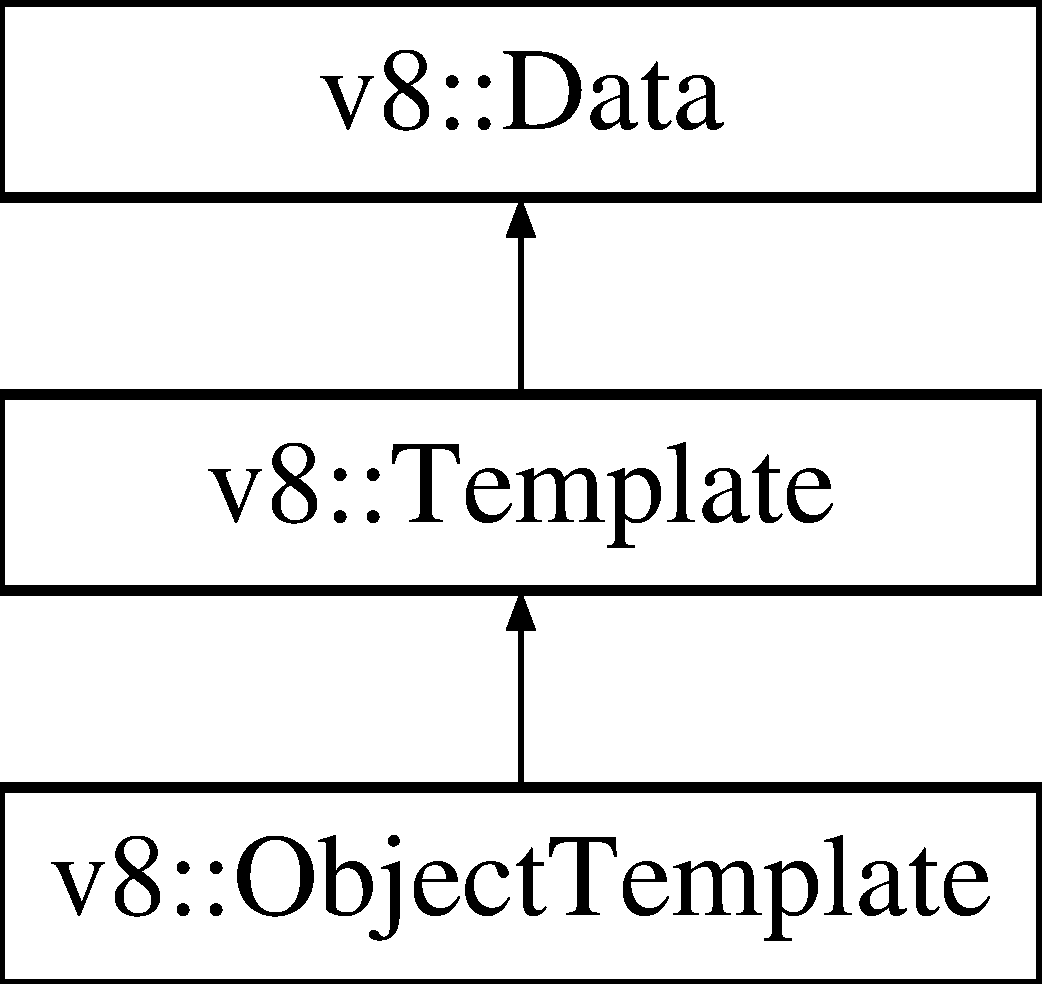
\includegraphics[height=3.000000cm]{classv8_1_1ObjectTemplate}
\end{center}
\end{figure}
\subsection*{Public Member Functions}
\begin{DoxyCompactItemize}
\item 
\hyperlink{classv8_1_1ObjectTemplate_abfa44addb7c9b426036a34bc7e60cc20}{V8\+\_\+\+D\+E\+P\+R\+E\+C\+A\+T\+E\+\_\+\+S\+O\+O\+N} (\char`\"{}Use maybe version\char`\"{}, Local$<$ \hyperlink{classv8_1_1Object}{Object} $>$ New\+Instance())
\item 
\hypertarget{classv8_1_1ObjectTemplate_ab6903ae25b5ffb081f1802df6b7fe6d7}{}V8\+\_\+\+W\+A\+R\+N\+\_\+\+U\+N\+U\+S\+E\+D\+\_\+\+R\+E\+S\+U\+L\+T \hyperlink{classv8_1_1MaybeLocal}{Maybe\+Local}$<$ \hyperlink{classv8_1_1Object}{Object} $>$ {\bfseries New\+Instance} (\hyperlink{classv8_1_1Local}{Local}$<$ \hyperlink{classv8_1_1Context}{Context} $>$ context)\label{classv8_1_1ObjectTemplate_ab6903ae25b5ffb081f1802df6b7fe6d7}

\item 
void \hyperlink{classv8_1_1ObjectTemplate_a7300126e15ff8246813e07f92d4fbe83}{Set\+Accessor} (\hyperlink{classv8_1_1Local}{Local}$<$ \hyperlink{classv8_1_1String}{String} $>$ name, \hyperlink{namespacev8_a722613c87061708a4f1aa050d095f868}{Accessor\+Getter\+Callback} getter, Accessor\+Setter\+Callback setter=0, \hyperlink{classv8_1_1Local}{Local}$<$ \hyperlink{classv8_1_1Value}{Value} $>$ data=\hyperlink{classv8_1_1Local}{Local}$<$ \hyperlink{classv8_1_1Value}{Value} $>$(), \hyperlink{namespacev8_a31d8355cb043d7d2dda3f4a52760b64e}{Access\+Control} settings=D\+E\+F\+A\+U\+L\+T, Property\+Attribute attribute=None, \hyperlink{classv8_1_1Local}{Local}$<$ \hyperlink{classv8_1_1AccessorSignature}{Accessor\+Signature} $>$ signature=\hyperlink{classv8_1_1Local}{Local}$<$ \hyperlink{classv8_1_1AccessorSignature}{Accessor\+Signature} $>$())
\item 
\hypertarget{classv8_1_1ObjectTemplate_a5efa63efe7659c138645eae226d30f2b}{}void {\bfseries Set\+Accessor} (\hyperlink{classv8_1_1Local}{Local}$<$ \hyperlink{classv8_1_1Name}{Name} $>$ name, Accessor\+Name\+Getter\+Callback getter, Accessor\+Name\+Setter\+Callback setter=0, \hyperlink{classv8_1_1Local}{Local}$<$ \hyperlink{classv8_1_1Value}{Value} $>$ data=\hyperlink{classv8_1_1Local}{Local}$<$ \hyperlink{classv8_1_1Value}{Value} $>$(), \hyperlink{namespacev8_a31d8355cb043d7d2dda3f4a52760b64e}{Access\+Control} settings=D\+E\+F\+A\+U\+L\+T, Property\+Attribute attribute=None, \hyperlink{classv8_1_1Local}{Local}$<$ \hyperlink{classv8_1_1AccessorSignature}{Accessor\+Signature} $>$ signature=\hyperlink{classv8_1_1Local}{Local}$<$ \hyperlink{classv8_1_1AccessorSignature}{Accessor\+Signature} $>$())\label{classv8_1_1ObjectTemplate_a5efa63efe7659c138645eae226d30f2b}

\item 
void \hyperlink{classv8_1_1ObjectTemplate_a66fa7b04c87676e20e35497ea09a0ad0}{Set\+Named\+Property\+Handler} (\hyperlink{namespacev8_a50cae386a68bf9ff23d02aa1161face4}{Named\+Property\+Getter\+Callback} getter, \hyperlink{namespacev8_a9587769513971dc7cb301b740d9e66b6}{Named\+Property\+Setter\+Callback} setter=0, \hyperlink{namespacev8_ac135beae5f0c8b290255accb438f990e}{Named\+Property\+Query\+Callback} query=0, \hyperlink{namespacev8_aaba861076c5b111912cfa0791d348437}{Named\+Property\+Deleter\+Callback} deleter=0, \hyperlink{namespacev8_a5f6f16818a9cddacadbfe6d90ca3a6b1}{Named\+Property\+Enumerator\+Callback} enumerator=0, \hyperlink{classv8_1_1Local}{Local}$<$ \hyperlink{classv8_1_1Value}{Value} $>$ data=\hyperlink{classv8_1_1Local}{Local}$<$ \hyperlink{classv8_1_1Value}{Value} $>$())
\item 
\hypertarget{classv8_1_1ObjectTemplate_a3d5666f1e9b0f46df6b4dbb7cfbb6114}{}void {\bfseries Set\+Handler} (const \hyperlink{structv8_1_1NamedPropertyHandlerConfiguration}{Named\+Property\+Handler\+Configuration} \&configuration)\label{classv8_1_1ObjectTemplate_a3d5666f1e9b0f46df6b4dbb7cfbb6114}

\item 
void \hyperlink{classv8_1_1ObjectTemplate_abc92c2889776a5a1ef6831f9c3da3783}{Set\+Handler} (const \hyperlink{structv8_1_1IndexedPropertyHandlerConfiguration}{Indexed\+Property\+Handler\+Configuration} \&configuration)
\item 
\hypertarget{classv8_1_1ObjectTemplate_ae3303f3d55370684ac02b02e67712eac}{}void {\bfseries Set\+Indexed\+Property\+Handler} (\hyperlink{namespacev8_a48e7816ba64447bf32a25d194588daaf}{Indexed\+Property\+Getter\+Callback} getter, \hyperlink{namespacev8_a4ac7cc6185ebc8b6a199f9fa8e6bf5c3}{Indexed\+Property\+Setter\+Callback} setter=0, \hyperlink{namespacev8_a980b62c33eb664783e61e25c3b27f9ee}{Indexed\+Property\+Query\+Callback} query=0, \hyperlink{namespacev8_a53863728de14cde48dd6543207b2f2da}{Indexed\+Property\+Deleter\+Callback} deleter=0, \hyperlink{namespacev8_adbb0a6d5537371953f9ba807d4f6275e}{Indexed\+Property\+Enumerator\+Callback} enumerator=0, \hyperlink{classv8_1_1Local}{Local}$<$ \hyperlink{classv8_1_1Value}{Value} $>$ data=\hyperlink{classv8_1_1Local}{Local}$<$ \hyperlink{classv8_1_1Value}{Value} $>$())\label{classv8_1_1ObjectTemplate_ae3303f3d55370684ac02b02e67712eac}

\item 
void \hyperlink{classv8_1_1ObjectTemplate_a1775c8f73e643c339804d2f5b628eddf}{Set\+Call\+As\+Function\+Handler} (Function\+Callback callback, \hyperlink{classv8_1_1Local}{Local}$<$ \hyperlink{classv8_1_1Value}{Value} $>$ data=\hyperlink{classv8_1_1Local}{Local}$<$ \hyperlink{classv8_1_1Value}{Value} $>$())
\item 
void \hyperlink{classv8_1_1ObjectTemplate_a7e40ef313b44c2ad336c73051523b4f8}{Mark\+As\+Undetectable} ()
\item 
void \hyperlink{classv8_1_1ObjectTemplate_a973635b9f6cad297cdc50ee67b07e20f}{Set\+Access\+Check\+Callbacks} (\hyperlink{namespacev8_ab5cafda0c556bba990c660ce9c904e0d}{Named\+Security\+Callback} named\+\_\+handler, \hyperlink{namespacev8_aebbcc7837753e51112d944ad96520da1}{Indexed\+Security\+Callback} indexed\+\_\+handler, \hyperlink{classv8_1_1Local}{Local}$<$ \hyperlink{classv8_1_1Value}{Value} $>$ data=\hyperlink{classv8_1_1Local}{Local}$<$ \hyperlink{classv8_1_1Value}{Value} $>$())
\item 
int \hyperlink{classv8_1_1ObjectTemplate_a43de785d594d8c01b18230b1aa79e31c}{Internal\+Field\+Count} ()
\item 
void \hyperlink{classv8_1_1ObjectTemplate_ab63916ac584a76bca8ba541f86ce9fce}{Set\+Internal\+Field\+Count} (int value)
\end{DoxyCompactItemize}
\subsection*{Static Public Member Functions}
\begin{DoxyCompactItemize}
\item 
static \hyperlink{classv8_1_1Local}{Local}$<$ \hyperlink{classv8_1_1ObjectTemplate}{Object\+Template} $>$ \hyperlink{classv8_1_1ObjectTemplate_ae0bcd58e9e069c50148c377d774de7a1}{New} (\hyperlink{classv8_1_1Isolate}{Isolate} $\ast$isolate, \hyperlink{classv8_1_1Local}{Local}$<$ \hyperlink{classv8_1_1FunctionTemplate}{Function\+Template} $>$ constructor=\hyperlink{classv8_1_1Local}{Local}$<$ \hyperlink{classv8_1_1FunctionTemplate}{Function\+Template} $>$())
\item 
\hypertarget{classv8_1_1ObjectTemplate_ade467a6adf3a65bfdef9e4db7ced8e0f}{}static {\bfseries V8\+\_\+\+D\+E\+P\+R\+E\+C\+A\+T\+E\+\_\+\+S\+O\+O\+N} (\char`\"{}Use isolate version\char`\"{}, Local$<$ \hyperlink{classv8_1_1ObjectTemplate}{Object\+Template} $>$ \hyperlink{classv8_1_1ObjectTemplate_ae0bcd58e9e069c50148c377d774de7a1}{New}())\label{classv8_1_1ObjectTemplate_ade467a6adf3a65bfdef9e4db7ced8e0f}

\end{DoxyCompactItemize}
\subsection*{Friends}
\begin{DoxyCompactItemize}
\item 
\hypertarget{classv8_1_1ObjectTemplate_a334168ad1a5f39cf17b818ca3356aacd}{}class {\bfseries Function\+Template}\label{classv8_1_1ObjectTemplate_a334168ad1a5f39cf17b818ca3356aacd}

\end{DoxyCompactItemize}


\subsection{Detailed Description}
An \hyperlink{classv8_1_1ObjectTemplate}{Object\+Template} is used to create objects at runtime.

Properties added to an \hyperlink{classv8_1_1ObjectTemplate}{Object\+Template} are added to each object created from the \hyperlink{classv8_1_1ObjectTemplate}{Object\+Template}. 

\subsection{Member Function Documentation}
\hypertarget{classv8_1_1ObjectTemplate_a43de785d594d8c01b18230b1aa79e31c}{}\index{v8\+::\+Object\+Template@{v8\+::\+Object\+Template}!Internal\+Field\+Count@{Internal\+Field\+Count}}
\index{Internal\+Field\+Count@{Internal\+Field\+Count}!v8\+::\+Object\+Template@{v8\+::\+Object\+Template}}
\subsubsection[{Internal\+Field\+Count}]{\setlength{\rightskip}{0pt plus 5cm}int v8\+::\+Object\+Template\+::\+Internal\+Field\+Count (
\begin{DoxyParamCaption}
{}
\end{DoxyParamCaption}
)}\label{classv8_1_1ObjectTemplate_a43de785d594d8c01b18230b1aa79e31c}
Gets the number of internal fields for objects generated from this template. \hypertarget{classv8_1_1ObjectTemplate_a7e40ef313b44c2ad336c73051523b4f8}{}\index{v8\+::\+Object\+Template@{v8\+::\+Object\+Template}!Mark\+As\+Undetectable@{Mark\+As\+Undetectable}}
\index{Mark\+As\+Undetectable@{Mark\+As\+Undetectable}!v8\+::\+Object\+Template@{v8\+::\+Object\+Template}}
\subsubsection[{Mark\+As\+Undetectable}]{\setlength{\rightskip}{0pt plus 5cm}void v8\+::\+Object\+Template\+::\+Mark\+As\+Undetectable (
\begin{DoxyParamCaption}
{}
\end{DoxyParamCaption}
)}\label{classv8_1_1ObjectTemplate_a7e40ef313b44c2ad336c73051523b4f8}
Mark object instances of the template as undetectable.

In many ways, undetectable objects behave as though they are not there. They behave like \textquotesingle{}undefined\textquotesingle{} in conditionals and when printed. However, properties can be accessed and called as on normal objects. \hypertarget{classv8_1_1ObjectTemplate_ae0bcd58e9e069c50148c377d774de7a1}{}\index{v8\+::\+Object\+Template@{v8\+::\+Object\+Template}!New@{New}}
\index{New@{New}!v8\+::\+Object\+Template@{v8\+::\+Object\+Template}}
\subsubsection[{New}]{\setlength{\rightskip}{0pt plus 5cm}static {\bf Local}$<${\bf Object\+Template}$>$ v8\+::\+Object\+Template\+::\+New (
\begin{DoxyParamCaption}
\item[{{\bf Isolate} $\ast$}]{isolate, }
\item[{{\bf Local}$<$ {\bf Function\+Template} $>$}]{constructor = {\ttfamily {\bf Local}$<$~{\bf Function\+Template}~$>$()}}
\end{DoxyParamCaption}
)\hspace{0.3cm}{\ttfamily [static]}}\label{classv8_1_1ObjectTemplate_ae0bcd58e9e069c50148c377d774de7a1}
Creates an \hyperlink{classv8_1_1ObjectTemplate}{Object\+Template}. \hypertarget{classv8_1_1ObjectTemplate_a973635b9f6cad297cdc50ee67b07e20f}{}\index{v8\+::\+Object\+Template@{v8\+::\+Object\+Template}!Set\+Access\+Check\+Callbacks@{Set\+Access\+Check\+Callbacks}}
\index{Set\+Access\+Check\+Callbacks@{Set\+Access\+Check\+Callbacks}!v8\+::\+Object\+Template@{v8\+::\+Object\+Template}}
\subsubsection[{Set\+Access\+Check\+Callbacks}]{\setlength{\rightskip}{0pt plus 5cm}void v8\+::\+Object\+Template\+::\+Set\+Access\+Check\+Callbacks (
\begin{DoxyParamCaption}
\item[{{\bf Named\+Security\+Callback}}]{named\+\_\+handler, }
\item[{{\bf Indexed\+Security\+Callback}}]{indexed\+\_\+handler, }
\item[{{\bf Local}$<$ {\bf Value} $>$}]{data = {\ttfamily {\bf Local}$<$~{\bf Value}~$>$()}}
\end{DoxyParamCaption}
)}\label{classv8_1_1ObjectTemplate_a973635b9f6cad297cdc50ee67b07e20f}
Sets access check callbacks on the object template and enables access checks.

When accessing properties on instances of this object template, the access check callback will be called to determine whether or not to allow cross-\/context access to the properties. \hypertarget{classv8_1_1ObjectTemplate_a7300126e15ff8246813e07f92d4fbe83}{}\index{v8\+::\+Object\+Template@{v8\+::\+Object\+Template}!Set\+Accessor@{Set\+Accessor}}
\index{Set\+Accessor@{Set\+Accessor}!v8\+::\+Object\+Template@{v8\+::\+Object\+Template}}
\subsubsection[{Set\+Accessor}]{\setlength{\rightskip}{0pt plus 5cm}void v8\+::\+Object\+Template\+::\+Set\+Accessor (
\begin{DoxyParamCaption}
\item[{{\bf Local}$<$ {\bf String} $>$}]{name, }
\item[{{\bf Accessor\+Getter\+Callback}}]{getter, }
\item[{Accessor\+Setter\+Callback}]{setter = {\ttfamily 0}, }
\item[{{\bf Local}$<$ {\bf Value} $>$}]{data = {\ttfamily {\bf Local}$<$~{\bf Value}~$>$()}, }
\item[{{\bf Access\+Control}}]{settings = {\ttfamily DEFAULT}, }
\item[{Property\+Attribute}]{attribute = {\ttfamily None}, }
\item[{{\bf Local}$<$ {\bf Accessor\+Signature} $>$}]{signature = {\ttfamily {\bf Local}$<$~{\bf Accessor\+Signature}~$>$()}}
\end{DoxyParamCaption}
)}\label{classv8_1_1ObjectTemplate_a7300126e15ff8246813e07f92d4fbe83}
Sets an accessor on the object template.

Whenever the property with the given name is accessed on objects created from this \hyperlink{classv8_1_1ObjectTemplate}{Object\+Template} the getter and setter callbacks are called instead of getting and setting the property directly on the Java\+Script object.


\begin{DoxyParams}{Parameters}
{\em name} & The name of the property for which an accessor is added. \\
\hline
{\em getter} & The callback to invoke when getting the property. \\
\hline
{\em setter} & The callback to invoke when setting the property. \\
\hline
{\em data} & A piece of data that will be passed to the getter and setter callbacks whenever they are invoked. \\
\hline
{\em settings} & Access control settings for the accessor. This is a bit field consisting of one of more of D\+E\+F\+A\+U\+L\+T = 0, A\+L\+L\+\_\+\+C\+A\+N\+\_\+\+R\+E\+A\+D = 1, or A\+L\+L\+\_\+\+C\+A\+N\+\_\+\+W\+R\+I\+T\+E = 2. The default is to not allow cross-\/context access. A\+L\+L\+\_\+\+C\+A\+N\+\_\+\+R\+E\+A\+D means that all cross-\/context reads are allowed. A\+L\+L\+\_\+\+C\+A\+N\+\_\+\+W\+R\+I\+T\+E means that all cross-\/context writes are allowed. The combination A\+L\+L\+\_\+\+C\+A\+N\+\_\+\+R\+E\+A\+D $\vert$ A\+L\+L\+\_\+\+C\+A\+N\+\_\+\+W\+R\+I\+T\+E can be used to allow all cross-\/context access. \\
\hline
{\em attribute} & The attributes of the property for which an accessor is added. \\
\hline
{\em signature} & The signature describes valid receivers for the accessor and is used to perform implicit instance checks against them. If the receiver is incompatible (i.\+e. is not an instance of the constructor as defined by \hyperlink{classv8_1_1FunctionTemplate_a90d838f3456d300bd19d2a2cb98645bd}{Function\+Template\+::\+Has\+Instance()}), an implicit Type\+Error is thrown and no callback is invoked. \\
\hline
\end{DoxyParams}
\hypertarget{classv8_1_1ObjectTemplate_a1775c8f73e643c339804d2f5b628eddf}{}\index{v8\+::\+Object\+Template@{v8\+::\+Object\+Template}!Set\+Call\+As\+Function\+Handler@{Set\+Call\+As\+Function\+Handler}}
\index{Set\+Call\+As\+Function\+Handler@{Set\+Call\+As\+Function\+Handler}!v8\+::\+Object\+Template@{v8\+::\+Object\+Template}}
\subsubsection[{Set\+Call\+As\+Function\+Handler}]{\setlength{\rightskip}{0pt plus 5cm}void v8\+::\+Object\+Template\+::\+Set\+Call\+As\+Function\+Handler (
\begin{DoxyParamCaption}
\item[{Function\+Callback}]{callback, }
\item[{{\bf Local}$<$ {\bf Value} $>$}]{data = {\ttfamily {\bf Local}$<$~{\bf Value}~$>$()}}
\end{DoxyParamCaption}
)}\label{classv8_1_1ObjectTemplate_a1775c8f73e643c339804d2f5b628eddf}
Sets the callback to be used when calling instances created from this template as a function. If no callback is set, instances behave like normal Java\+Script objects that cannot be called as a function. \hypertarget{classv8_1_1ObjectTemplate_abc92c2889776a5a1ef6831f9c3da3783}{}\index{v8\+::\+Object\+Template@{v8\+::\+Object\+Template}!Set\+Handler@{Set\+Handler}}
\index{Set\+Handler@{Set\+Handler}!v8\+::\+Object\+Template@{v8\+::\+Object\+Template}}
\subsubsection[{Set\+Handler}]{\setlength{\rightskip}{0pt plus 5cm}void v8\+::\+Object\+Template\+::\+Set\+Handler (
\begin{DoxyParamCaption}
\item[{const {\bf Indexed\+Property\+Handler\+Configuration} \&}]{configuration}
\end{DoxyParamCaption}
)}\label{classv8_1_1ObjectTemplate_abc92c2889776a5a1ef6831f9c3da3783}
Sets an indexed property handler on the object template.

Whenever an indexed property is accessed on objects created from this object template, the provided callback is invoked instead of accessing the property directly on the Java\+Script object.


\begin{DoxyParams}{Parameters}
{\em getter} & The callback to invoke when getting a property. \\
\hline
{\em setter} & The callback to invoke when setting a property. \\
\hline
{\em query} & The callback to invoke to check if an object has a property. \\
\hline
{\em deleter} & The callback to invoke when deleting a property. \\
\hline
{\em enumerator} & The callback to invoke to enumerate all the indexed properties of an object. \\
\hline
{\em data} & A piece of data that will be passed to the callbacks whenever they are invoked. \\
\hline
\end{DoxyParams}
\hypertarget{classv8_1_1ObjectTemplate_ab63916ac584a76bca8ba541f86ce9fce}{}\index{v8\+::\+Object\+Template@{v8\+::\+Object\+Template}!Set\+Internal\+Field\+Count@{Set\+Internal\+Field\+Count}}
\index{Set\+Internal\+Field\+Count@{Set\+Internal\+Field\+Count}!v8\+::\+Object\+Template@{v8\+::\+Object\+Template}}
\subsubsection[{Set\+Internal\+Field\+Count}]{\setlength{\rightskip}{0pt plus 5cm}void v8\+::\+Object\+Template\+::\+Set\+Internal\+Field\+Count (
\begin{DoxyParamCaption}
\item[{int}]{value}
\end{DoxyParamCaption}
)}\label{classv8_1_1ObjectTemplate_ab63916ac584a76bca8ba541f86ce9fce}
Sets the number of internal fields for objects generated from this template. \hypertarget{classv8_1_1ObjectTemplate_a66fa7b04c87676e20e35497ea09a0ad0}{}\index{v8\+::\+Object\+Template@{v8\+::\+Object\+Template}!Set\+Named\+Property\+Handler@{Set\+Named\+Property\+Handler}}
\index{Set\+Named\+Property\+Handler@{Set\+Named\+Property\+Handler}!v8\+::\+Object\+Template@{v8\+::\+Object\+Template}}
\subsubsection[{Set\+Named\+Property\+Handler}]{\setlength{\rightskip}{0pt plus 5cm}void v8\+::\+Object\+Template\+::\+Set\+Named\+Property\+Handler (
\begin{DoxyParamCaption}
\item[{{\bf Named\+Property\+Getter\+Callback}}]{getter, }
\item[{{\bf Named\+Property\+Setter\+Callback}}]{setter = {\ttfamily 0}, }
\item[{{\bf Named\+Property\+Query\+Callback}}]{query = {\ttfamily 0}, }
\item[{{\bf Named\+Property\+Deleter\+Callback}}]{deleter = {\ttfamily 0}, }
\item[{{\bf Named\+Property\+Enumerator\+Callback}}]{enumerator = {\ttfamily 0}, }
\item[{{\bf Local}$<$ {\bf Value} $>$}]{data = {\ttfamily {\bf Local}$<$~{\bf Value}~$>$()}}
\end{DoxyParamCaption}
)}\label{classv8_1_1ObjectTemplate_a66fa7b04c87676e20e35497ea09a0ad0}
Sets a named property handler on the object template.

Whenever a property whose name is a string is accessed on objects created from this object template, the provided callback is invoked instead of accessing the property directly on the Java\+Script object.

Note that new code should use the second version that can intercept symbol-\/named properties as well as string-\/named properties.


\begin{DoxyParams}{Parameters}
{\em getter} & The callback to invoke when getting a property. \\
\hline
{\em setter} & The callback to invoke when setting a property. \\
\hline
{\em query} & The callback to invoke to check if a property is present, and if present, get its attributes. \\
\hline
{\em deleter} & The callback to invoke when deleting a property. \\
\hline
{\em enumerator} & The callback to invoke to enumerate all the named properties of an object. \\
\hline
{\em data} & A piece of data that will be passed to the callbacks whenever they are invoked. \\
\hline
\end{DoxyParams}
\hypertarget{classv8_1_1ObjectTemplate_abfa44addb7c9b426036a34bc7e60cc20}{}\index{v8\+::\+Object\+Template@{v8\+::\+Object\+Template}!V8\+\_\+\+D\+E\+P\+R\+E\+C\+A\+T\+E\+\_\+\+S\+O\+O\+N@{V8\+\_\+\+D\+E\+P\+R\+E\+C\+A\+T\+E\+\_\+\+S\+O\+O\+N}}
\index{V8\+\_\+\+D\+E\+P\+R\+E\+C\+A\+T\+E\+\_\+\+S\+O\+O\+N@{V8\+\_\+\+D\+E\+P\+R\+E\+C\+A\+T\+E\+\_\+\+S\+O\+O\+N}!v8\+::\+Object\+Template@{v8\+::\+Object\+Template}}
\subsubsection[{V8\+\_\+\+D\+E\+P\+R\+E\+C\+A\+T\+E\+\_\+\+S\+O\+O\+N}]{\setlength{\rightskip}{0pt plus 5cm}v8\+::\+Object\+Template\+::\+V8\+\_\+\+D\+E\+P\+R\+E\+C\+A\+T\+E\+\_\+\+S\+O\+O\+N (
\begin{DoxyParamCaption}
\item[{\char`\"{}Use maybe version\char`\"{}}]{, }
\item[{{\bf Local}$<$ {\bf Object} $>$ }]{New\+Instance()}
\end{DoxyParamCaption}
)}\label{classv8_1_1ObjectTemplate_abfa44addb7c9b426036a34bc7e60cc20}
Creates a new instance of this template. 

The documentation for this class was generated from the following file\+:\begin{DoxyCompactItemize}
\item 
v8/include/v8.\+h\end{DoxyCompactItemize}

\hypertarget{classv8_1_1OutputStream}{}\section{v8\+:\+:Output\+Stream Class Reference}
\label{classv8_1_1OutputStream}\index{v8\+::\+Output\+Stream@{v8\+::\+Output\+Stream}}


{\ttfamily \#include $<$v8-\/profiler.\+h$>$}

\subsection*{Public Types}
\begin{DoxyCompactItemize}
\item 
enum {\bfseries Write\+Result} \{ {\bfseries k\+Continue} = 0, 
{\bfseries k\+Abort} = 1
 \}\hypertarget{classv8_1_1OutputStream_a336c7605a0ce4fbe6f6fca3b03bc16de}{}\label{classv8_1_1OutputStream_a336c7605a0ce4fbe6f6fca3b03bc16de}

\end{DoxyCompactItemize}
\subsection*{Public Member Functions}
\begin{DoxyCompactItemize}
\item 
virtual void \hyperlink{classv8_1_1OutputStream_a6c5c308367fc5776bcbedff0e94d6049}{End\+Of\+Stream} ()=0
\item 
virtual int \hyperlink{classv8_1_1OutputStream_a93bdaa790cbd66a7283fad2cca3f48f7}{Get\+Chunk\+Size} ()
\item 
virtual Write\+Result \hyperlink{classv8_1_1OutputStream_a42adc62ebe43d00159f80328538f217f}{Write\+Ascii\+Chunk} (char $\ast$data, int size)=0
\item 
virtual Write\+Result \hyperlink{classv8_1_1OutputStream_a104fd1a0b5ef685e1d4967aaacbb9e9d}{Write\+Heap\+Stats\+Chunk} (\hyperlink{structv8_1_1HeapStatsUpdate}{Heap\+Stats\+Update} $\ast$data, int count)
\end{DoxyCompactItemize}


\subsection{Detailed Description}
An interface for exporting data from \hyperlink{classv8_1_1V8}{V8}, using \char`\"{}push\char`\"{} model. 

\subsection{Member Function Documentation}
\index{v8\+::\+Output\+Stream@{v8\+::\+Output\+Stream}!End\+Of\+Stream@{End\+Of\+Stream}}
\index{End\+Of\+Stream@{End\+Of\+Stream}!v8\+::\+Output\+Stream@{v8\+::\+Output\+Stream}}
\subsubsection[{\texorpdfstring{End\+Of\+Stream()=0}{EndOfStream()=0}}]{\setlength{\rightskip}{0pt plus 5cm}virtual void v8\+::\+Output\+Stream\+::\+End\+Of\+Stream (
\begin{DoxyParamCaption}
{}
\end{DoxyParamCaption}
)\hspace{0.3cm}{\ttfamily [pure virtual]}}\hypertarget{classv8_1_1OutputStream_a6c5c308367fc5776bcbedff0e94d6049}{}\label{classv8_1_1OutputStream_a6c5c308367fc5776bcbedff0e94d6049}
Notify about the end of stream. \index{v8\+::\+Output\+Stream@{v8\+::\+Output\+Stream}!Get\+Chunk\+Size@{Get\+Chunk\+Size}}
\index{Get\+Chunk\+Size@{Get\+Chunk\+Size}!v8\+::\+Output\+Stream@{v8\+::\+Output\+Stream}}
\subsubsection[{\texorpdfstring{Get\+Chunk\+Size()}{GetChunkSize()}}]{\setlength{\rightskip}{0pt plus 5cm}virtual int v8\+::\+Output\+Stream\+::\+Get\+Chunk\+Size (
\begin{DoxyParamCaption}
{}
\end{DoxyParamCaption}
)\hspace{0.3cm}{\ttfamily [inline]}, {\ttfamily [virtual]}}\hypertarget{classv8_1_1OutputStream_a93bdaa790cbd66a7283fad2cca3f48f7}{}\label{classv8_1_1OutputStream_a93bdaa790cbd66a7283fad2cca3f48f7}
Get preferred output chunk size. Called only once. \index{v8\+::\+Output\+Stream@{v8\+::\+Output\+Stream}!Write\+Ascii\+Chunk@{Write\+Ascii\+Chunk}}
\index{Write\+Ascii\+Chunk@{Write\+Ascii\+Chunk}!v8\+::\+Output\+Stream@{v8\+::\+Output\+Stream}}
\subsubsection[{\texorpdfstring{Write\+Ascii\+Chunk(char $\ast$data, int size)=0}{WriteAsciiChunk(char *data, int size)=0}}]{\setlength{\rightskip}{0pt plus 5cm}virtual Write\+Result v8\+::\+Output\+Stream\+::\+Write\+Ascii\+Chunk (
\begin{DoxyParamCaption}
\item[{char $\ast$}]{data, }
\item[{int}]{size}
\end{DoxyParamCaption}
)\hspace{0.3cm}{\ttfamily [pure virtual]}}\hypertarget{classv8_1_1OutputStream_a42adc62ebe43d00159f80328538f217f}{}\label{classv8_1_1OutputStream_a42adc62ebe43d00159f80328538f217f}
Writes the next chunk of snapshot data into the stream. Writing can be stopped by returning k\+Abort as function result. End\+Of\+Stream will not be called in case writing was aborted. \index{v8\+::\+Output\+Stream@{v8\+::\+Output\+Stream}!Write\+Heap\+Stats\+Chunk@{Write\+Heap\+Stats\+Chunk}}
\index{Write\+Heap\+Stats\+Chunk@{Write\+Heap\+Stats\+Chunk}!v8\+::\+Output\+Stream@{v8\+::\+Output\+Stream}}
\subsubsection[{\texorpdfstring{Write\+Heap\+Stats\+Chunk(\+Heap\+Stats\+Update $\ast$data, int count)}{WriteHeapStatsChunk(HeapStatsUpdate *data, int count)}}]{\setlength{\rightskip}{0pt plus 5cm}virtual Write\+Result v8\+::\+Output\+Stream\+::\+Write\+Heap\+Stats\+Chunk (
\begin{DoxyParamCaption}
\item[{{\bf Heap\+Stats\+Update} $\ast$}]{data, }
\item[{int}]{count}
\end{DoxyParamCaption}
)\hspace{0.3cm}{\ttfamily [inline]}, {\ttfamily [virtual]}}\hypertarget{classv8_1_1OutputStream_a104fd1a0b5ef685e1d4967aaacbb9e9d}{}\label{classv8_1_1OutputStream_a104fd1a0b5ef685e1d4967aaacbb9e9d}
Writes the next chunk of heap stats data into the stream. Writing can be stopped by returning k\+Abort as function result. End\+Of\+Stream will not be called in case writing was aborted. 

The documentation for this class was generated from the following file\+:\begin{DoxyCompactItemize}
\item 
v8/include/v8-\/profiler.\+h\end{DoxyCompactItemize}

\hypertarget{classv8_1_1Persistent}{}\section{v8\+:\+:Persistent$<$ T, M $>$ Class Template Reference}
\label{classv8_1_1Persistent}\index{v8\+::\+Persistent$<$ T, M $>$@{v8\+::\+Persistent$<$ T, M $>$}}


{\ttfamily \#include $<$v8.\+h$>$}

Inheritance diagram for v8\+:\+:Persistent$<$ T, M $>$\+:\begin{figure}[H]
\begin{center}
\leavevmode
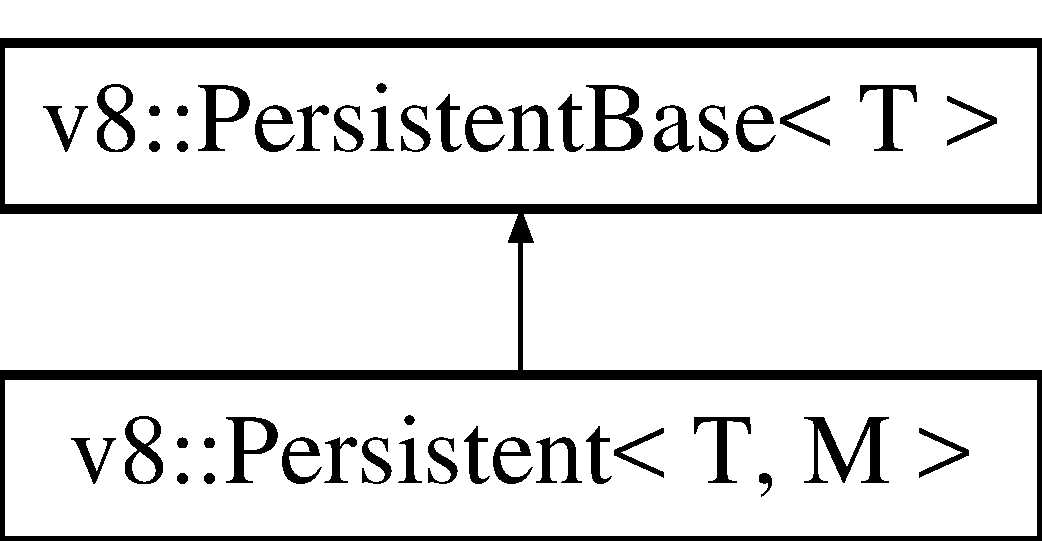
\includegraphics[height=2.000000cm]{classv8_1_1Persistent}
\end{center}
\end{figure}
\subsection*{Public Member Functions}
\begin{DoxyCompactItemize}
\item 
V8\+\_\+\+I\+N\+L\+I\+NE \mbox{\hyperlink{classv8_1_1Persistent_a5ce14612215393683d814056015a102d}{Persistent}} ()
\item 
{\footnotesize template$<$class S $>$ }\\V8\+\_\+\+I\+N\+L\+I\+NE \mbox{\hyperlink{classv8_1_1Persistent_aabe9a42d7971bd31173bca34186d9ac2}{Persistent}} (\mbox{\hyperlink{classv8_1_1Isolate}{Isolate}} $\ast$isolate, \mbox{\hyperlink{classv8_1_1Local}{Local}}$<$ S $>$ that)
\item 
{\footnotesize template$<$class S , class M2 $>$ }\\V8\+\_\+\+I\+N\+L\+I\+NE \mbox{\hyperlink{classv8_1_1Persistent_aaf9eb7c4e6d0ef2c81a2c08238653578}{Persistent}} (\mbox{\hyperlink{classv8_1_1Isolate}{Isolate}} $\ast$isolate, const \mbox{\hyperlink{classv8_1_1Persistent}{Persistent}}$<$ S, M2 $>$ \&that)
\item 
V8\+\_\+\+I\+N\+L\+I\+NE \mbox{\hyperlink{classv8_1_1Persistent_a22331e91572784cd5ed5519739bb50c7}{Persistent}} (const \mbox{\hyperlink{classv8_1_1Persistent}{Persistent}} \&that)
\item 
\mbox{\Hypertarget{classv8_1_1Persistent_ace17fd143fb6414d305871bf0a53ef57}\label{classv8_1_1Persistent_ace17fd143fb6414d305871bf0a53ef57}} 
{\footnotesize template$<$class S , class M2 $>$ }\\V8\+\_\+\+I\+N\+L\+I\+NE {\bfseries Persistent} (const \mbox{\hyperlink{classv8_1_1Persistent}{Persistent}}$<$ S, M2 $>$ \&that)
\item 
\mbox{\Hypertarget{classv8_1_1Persistent_aa1db9923b3212fb8ce57868217858b39}\label{classv8_1_1Persistent_aa1db9923b3212fb8ce57868217858b39}} 
V8\+\_\+\+I\+N\+L\+I\+NE \mbox{\hyperlink{classv8_1_1Persistent}{Persistent}} \& {\bfseries operator=} (const \mbox{\hyperlink{classv8_1_1Persistent}{Persistent}} \&that)
\item 
\mbox{\Hypertarget{classv8_1_1Persistent_a11104ee8739cb1f25e40fd17d746b48f}\label{classv8_1_1Persistent_a11104ee8739cb1f25e40fd17d746b48f}} 
{\footnotesize template$<$class S , class M2 $>$ }\\V8\+\_\+\+I\+N\+L\+I\+NE \mbox{\hyperlink{classv8_1_1Persistent}{Persistent}} \& {\bfseries operator=} (const \mbox{\hyperlink{classv8_1_1Persistent}{Persistent}}$<$ S, M2 $>$ \&that)
\item 
V8\+\_\+\+I\+N\+L\+I\+NE \mbox{\hyperlink{classv8_1_1Persistent_a7d4d2bebfe3919e447e22adc15464e25}{$\sim$\+Persistent}} ()
\item 
\mbox{\Hypertarget{classv8_1_1Persistent_a842282b8cb50699f99c5e415230926ee}\label{classv8_1_1Persistent_a842282b8cb50699f99c5e415230926ee}} 
{\footnotesize template$<$class S $>$ }\\V8\+\_\+\+I\+N\+L\+I\+NE \mbox{\hyperlink{classv8_1_1Persistent}{Persistent}}$<$ S $>$ \& {\bfseries As} () const
\item 
\mbox{\Hypertarget{classv8_1_1Persistent_ace50a178e3b772f75611e22e41fae974}\label{classv8_1_1Persistent_ace50a178e3b772f75611e22e41fae974}} 
{\footnotesize template$<$class S , class M2 $>$ }\\void {\bfseries Copy} (const \mbox{\hyperlink{classv8_1_1Persistent}{Persistent}}$<$ S, M2 $>$ \&that)
\end{DoxyCompactItemize}
\subsection*{Static Public Member Functions}
\begin{DoxyCompactItemize}
\item 
\mbox{\Hypertarget{classv8_1_1Persistent_aefcf5962630a14c198f466f64a685946}\label{classv8_1_1Persistent_aefcf5962630a14c198f466f64a685946}} 
{\footnotesize template$<$class S $>$ }\\static V8\+\_\+\+I\+N\+L\+I\+NE \mbox{\hyperlink{classv8_1_1Persistent}{Persistent}}$<$ T $>$ \& {\bfseries Cast} (const \mbox{\hyperlink{classv8_1_1Persistent}{Persistent}}$<$ S $>$ \&that)
\end{DoxyCompactItemize}
\subsection*{Friends}
\begin{DoxyCompactItemize}
\item 
\mbox{\Hypertarget{classv8_1_1Persistent_aba4f0964bdacf2bbf62cf876e5d28d0a}\label{classv8_1_1Persistent_aba4f0964bdacf2bbf62cf876e5d28d0a}} 
class {\bfseries Isolate}
\item 
\mbox{\Hypertarget{classv8_1_1Persistent_abc0f7da619e9e72510dc07ed7b5ff6d8}\label{classv8_1_1Persistent_abc0f7da619e9e72510dc07ed7b5ff6d8}} 
class {\bfseries Utils}
\item 
\mbox{\Hypertarget{classv8_1_1Persistent_afb872edb4aac7ba55f0da004113aa2b0}\label{classv8_1_1Persistent_afb872edb4aac7ba55f0da004113aa2b0}} 
{\footnotesize template$<$class F $>$ }\\class {\bfseries Local}
\item 
\mbox{\Hypertarget{classv8_1_1Persistent_ad845ec8872174be0a9ca9a3dd1898d30}\label{classv8_1_1Persistent_ad845ec8872174be0a9ca9a3dd1898d30}} 
{\footnotesize template$<$class F1 , class F2 $>$ }\\class {\bfseries Persistent}
\item 
\mbox{\Hypertarget{classv8_1_1Persistent_a53f604d3d6f2dc0647df33c9979f116a}\label{classv8_1_1Persistent_a53f604d3d6f2dc0647df33c9979f116a}} 
{\footnotesize template$<$class F $>$ }\\class {\bfseries Return\+Value}
\end{DoxyCompactItemize}


\subsection{Detailed Description}
\subsubsection*{template$<$class T, class M$>$\newline
class v8\+::\+Persistent$<$ T, M $>$}

A \mbox{\hyperlink{classv8_1_1PersistentBase}{Persistent\+Base}} which allows copy and assignment.

Copy, assignment and destructor behavior is controlled by the traits class M.

Note\+: \mbox{\hyperlink{classv8_1_1Persistent}{Persistent}} class hierarchy is subject to future changes. 

\subsection{Constructor \& Destructor Documentation}
\mbox{\Hypertarget{classv8_1_1Persistent_a5ce14612215393683d814056015a102d}\label{classv8_1_1Persistent_a5ce14612215393683d814056015a102d}} 
\index{v8\+::\+Persistent@{v8\+::\+Persistent}!Persistent@{Persistent}}
\index{Persistent@{Persistent}!v8\+::\+Persistent@{v8\+::\+Persistent}}
\subsubsection{\texorpdfstring{Persistent()}{Persistent()}\hspace{0.1cm}{\footnotesize\ttfamily [1/4]}}
{\footnotesize\ttfamily template$<$class T, class M$>$ \\
V8\+\_\+\+I\+N\+L\+I\+NE \mbox{\hyperlink{classv8_1_1Persistent}{v8\+::\+Persistent}}$<$ T, M $>$\+::\mbox{\hyperlink{classv8_1_1Persistent}{Persistent}} (\begin{DoxyParamCaption}{ }\end{DoxyParamCaption})\hspace{0.3cm}{\ttfamily [inline]}}

A \mbox{\hyperlink{classv8_1_1Persistent}{Persistent}} with no storage cell. \mbox{\Hypertarget{classv8_1_1Persistent_aabe9a42d7971bd31173bca34186d9ac2}\label{classv8_1_1Persistent_aabe9a42d7971bd31173bca34186d9ac2}} 
\index{v8\+::\+Persistent@{v8\+::\+Persistent}!Persistent@{Persistent}}
\index{Persistent@{Persistent}!v8\+::\+Persistent@{v8\+::\+Persistent}}
\subsubsection{\texorpdfstring{Persistent()}{Persistent()}\hspace{0.1cm}{\footnotesize\ttfamily [2/4]}}
{\footnotesize\ttfamily template$<$class T, class M$>$ \\
template$<$class S $>$ \\
V8\+\_\+\+I\+N\+L\+I\+NE \mbox{\hyperlink{classv8_1_1Persistent}{v8\+::\+Persistent}}$<$ T, M $>$\+::\mbox{\hyperlink{classv8_1_1Persistent}{Persistent}} (\begin{DoxyParamCaption}\item[{\mbox{\hyperlink{classv8_1_1Isolate}{Isolate}} $\ast$}]{isolate,  }\item[{\mbox{\hyperlink{classv8_1_1Local}{Local}}$<$ S $>$}]{that }\end{DoxyParamCaption})\hspace{0.3cm}{\ttfamily [inline]}}

Construct a \mbox{\hyperlink{classv8_1_1Persistent}{Persistent}} from a \mbox{\hyperlink{classv8_1_1Local}{Local}}. When the \mbox{\hyperlink{classv8_1_1Local}{Local}} is non-\/empty, a new storage cell is created pointing to the same object, and no flags are set. \mbox{\Hypertarget{classv8_1_1Persistent_aaf9eb7c4e6d0ef2c81a2c08238653578}\label{classv8_1_1Persistent_aaf9eb7c4e6d0ef2c81a2c08238653578}} 
\index{v8\+::\+Persistent@{v8\+::\+Persistent}!Persistent@{Persistent}}
\index{Persistent@{Persistent}!v8\+::\+Persistent@{v8\+::\+Persistent}}
\subsubsection{\texorpdfstring{Persistent()}{Persistent()}\hspace{0.1cm}{\footnotesize\ttfamily [3/4]}}
{\footnotesize\ttfamily template$<$class T, class M$>$ \\
template$<$class S , class M2 $>$ \\
V8\+\_\+\+I\+N\+L\+I\+NE \mbox{\hyperlink{classv8_1_1Persistent}{v8\+::\+Persistent}}$<$ T, M $>$\+::\mbox{\hyperlink{classv8_1_1Persistent}{Persistent}} (\begin{DoxyParamCaption}\item[{\mbox{\hyperlink{classv8_1_1Isolate}{Isolate}} $\ast$}]{isolate,  }\item[{const \mbox{\hyperlink{classv8_1_1Persistent}{Persistent}}$<$ S, M2 $>$ \&}]{that }\end{DoxyParamCaption})\hspace{0.3cm}{\ttfamily [inline]}}

Construct a \mbox{\hyperlink{classv8_1_1Persistent}{Persistent}} from a \mbox{\hyperlink{classv8_1_1Persistent}{Persistent}}. When the \mbox{\hyperlink{classv8_1_1Persistent}{Persistent}} is non-\/empty, a new storage cell is created pointing to the same object, and no flags are set. \mbox{\Hypertarget{classv8_1_1Persistent_a22331e91572784cd5ed5519739bb50c7}\label{classv8_1_1Persistent_a22331e91572784cd5ed5519739bb50c7}} 
\index{v8\+::\+Persistent@{v8\+::\+Persistent}!Persistent@{Persistent}}
\index{Persistent@{Persistent}!v8\+::\+Persistent@{v8\+::\+Persistent}}
\subsubsection{\texorpdfstring{Persistent()}{Persistent()}\hspace{0.1cm}{\footnotesize\ttfamily [4/4]}}
{\footnotesize\ttfamily template$<$class T, class M$>$ \\
V8\+\_\+\+I\+N\+L\+I\+NE \mbox{\hyperlink{classv8_1_1Persistent}{v8\+::\+Persistent}}$<$ T, M $>$\+::\mbox{\hyperlink{classv8_1_1Persistent}{Persistent}} (\begin{DoxyParamCaption}\item[{const \mbox{\hyperlink{classv8_1_1Persistent}{Persistent}}$<$ T, M $>$ \&}]{that }\end{DoxyParamCaption})\hspace{0.3cm}{\ttfamily [inline]}}

The copy constructors and assignment operator create a \mbox{\hyperlink{classv8_1_1Persistent}{Persistent}} exactly as the \mbox{\hyperlink{classv8_1_1Persistent}{Persistent}} constructor, but the Copy function from the traits class is called, allowing the setting of flags based on the copied \mbox{\hyperlink{classv8_1_1Persistent}{Persistent}}. \mbox{\Hypertarget{classv8_1_1Persistent_a7d4d2bebfe3919e447e22adc15464e25}\label{classv8_1_1Persistent_a7d4d2bebfe3919e447e22adc15464e25}} 
\index{v8\+::\+Persistent@{v8\+::\+Persistent}!````~Persistent@{$\sim$\+Persistent}}
\index{````~Persistent@{$\sim$\+Persistent}!v8\+::\+Persistent@{v8\+::\+Persistent}}
\subsubsection{\texorpdfstring{$\sim$\+Persistent()}{~Persistent()}}
{\footnotesize\ttfamily template$<$class T, class M$>$ \\
V8\+\_\+\+I\+N\+L\+I\+NE \mbox{\hyperlink{classv8_1_1Persistent}{v8\+::\+Persistent}}$<$ T, M $>$\+::$\sim$\mbox{\hyperlink{classv8_1_1Persistent}{Persistent}} (\begin{DoxyParamCaption}{ }\end{DoxyParamCaption})\hspace{0.3cm}{\ttfamily [inline]}}

The destructor will dispose the \mbox{\hyperlink{classv8_1_1Persistent}{Persistent}} based on the k\+Reset\+In\+Destructor flags in the traits class. Since not calling dispose can result in a memory leak, it is recommended to always set this flag. 

The documentation for this class was generated from the following file\+:\begin{DoxyCompactItemize}
\item 
v8/include/v8.\+h\end{DoxyCompactItemize}

\hypertarget{classv8_1_1PersistentBase}{}\section{v8\+:\+:Persistent\+Base$<$ T $>$ Class Template Reference}
\label{classv8_1_1PersistentBase}\index{v8\+::\+Persistent\+Base$<$ T $>$@{v8\+::\+Persistent\+Base$<$ T $>$}}


{\ttfamily \#include $<$v8.\+h$>$}

Inheritance diagram for v8\+:\+:Persistent\+Base$<$ T $>$\+:\begin{figure}[H]
\begin{center}
\leavevmode
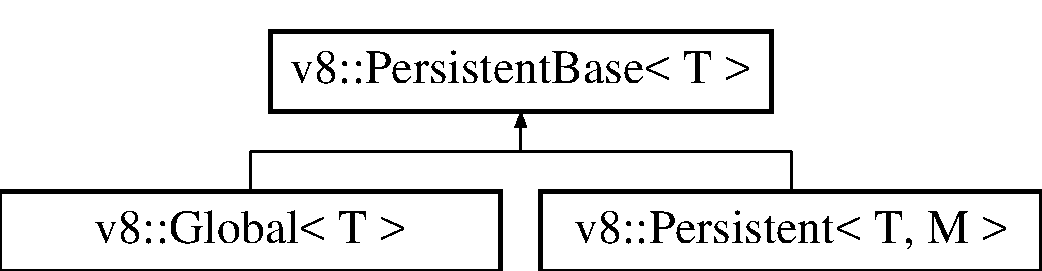
\includegraphics[height=2.000000cm]{classv8_1_1PersistentBase}
\end{center}
\end{figure}
\subsection*{Public Member Functions}
\begin{DoxyCompactItemize}
\item 
V8\+\_\+\+I\+N\+L\+I\+NE void \mbox{\hyperlink{classv8_1_1PersistentBase_a174bb1e45b18fd4eeaee033622825bb8}{Reset}} ()
\item 
{\footnotesize template$<$class S $>$ }\\V8\+\_\+\+I\+N\+L\+I\+NE void \mbox{\hyperlink{classv8_1_1PersistentBase_a11164f0dfc9a16d79809236e7a9670aa}{Reset}} (Isolate $\ast$isolate, const \mbox{\hyperlink{classv8_1_1Local}{Local}}$<$ S $>$ \&other)
\item 
{\footnotesize template$<$class S $>$ }\\V8\+\_\+\+I\+N\+L\+I\+NE void \mbox{\hyperlink{classv8_1_1PersistentBase_af6b8f929b0cbaa83341df48ca3b03ef5}{Reset}} (Isolate $\ast$isolate, const \mbox{\hyperlink{classv8_1_1PersistentBase}{Persistent\+Base}}$<$ S $>$ \&other)
\item 
\mbox{\Hypertarget{classv8_1_1PersistentBase_aa4d270d1946260813a4fba08121fdbd1}\label{classv8_1_1PersistentBase_aa4d270d1946260813a4fba08121fdbd1}} 
V8\+\_\+\+I\+N\+L\+I\+NE bool {\bfseries Is\+Empty} () const
\item 
\mbox{\Hypertarget{classv8_1_1PersistentBase_abb8a06471ea86de1731a3c94a879b00e}\label{classv8_1_1PersistentBase_abb8a06471ea86de1731a3c94a879b00e}} 
V8\+\_\+\+I\+N\+L\+I\+NE void {\bfseries Empty} ()
\item 
\mbox{\Hypertarget{classv8_1_1PersistentBase_ae943e4070eb5d18493575b37a0cfb6f8}\label{classv8_1_1PersistentBase_ae943e4070eb5d18493575b37a0cfb6f8}} 
V8\+\_\+\+I\+N\+L\+I\+NE \mbox{\hyperlink{classv8_1_1Local}{Local}}$<$ T $>$ {\bfseries Get} (Isolate $\ast$isolate) const
\item 
\mbox{\Hypertarget{classv8_1_1PersistentBase_a2a267a582638e2acc864f672b25e4b9c}\label{classv8_1_1PersistentBase_a2a267a582638e2acc864f672b25e4b9c}} 
{\footnotesize template$<$class S $>$ }\\V8\+\_\+\+I\+N\+L\+I\+NE bool {\bfseries operator==} (const \mbox{\hyperlink{classv8_1_1PersistentBase}{Persistent\+Base}}$<$ S $>$ \&that) const
\item 
\mbox{\Hypertarget{classv8_1_1PersistentBase_a4a2ec8bcbe0fe95cac2e3c17b800557e}\label{classv8_1_1PersistentBase_a4a2ec8bcbe0fe95cac2e3c17b800557e}} 
{\footnotesize template$<$class S $>$ }\\V8\+\_\+\+I\+N\+L\+I\+NE bool {\bfseries operator==} (const \mbox{\hyperlink{classv8_1_1Local}{Local}}$<$ S $>$ \&that) const
\item 
\mbox{\Hypertarget{classv8_1_1PersistentBase_a2893d38e56559c016e33e832b814a515}\label{classv8_1_1PersistentBase_a2893d38e56559c016e33e832b814a515}} 
{\footnotesize template$<$class S $>$ }\\V8\+\_\+\+I\+N\+L\+I\+NE bool {\bfseries operator!=} (const \mbox{\hyperlink{classv8_1_1PersistentBase}{Persistent\+Base}}$<$ S $>$ \&that) const
\item 
\mbox{\Hypertarget{classv8_1_1PersistentBase_a6bfcb31182bcc9a2cc20b83807f7fb45}\label{classv8_1_1PersistentBase_a6bfcb31182bcc9a2cc20b83807f7fb45}} 
{\footnotesize template$<$class S $>$ }\\V8\+\_\+\+I\+N\+L\+I\+NE bool {\bfseries operator!=} (const \mbox{\hyperlink{classv8_1_1Local}{Local}}$<$ S $>$ \&that) const
\item 
{\footnotesize template$<$typename P $>$ }\\V8\+\_\+\+I\+N\+L\+I\+NE void \mbox{\hyperlink{classv8_1_1PersistentBase_aebb8a2c97e219102f613ff3749c956f6}{Set\+Weak}} (P $\ast$parameter, typename \mbox{\hyperlink{classv8_1_1WeakCallbackInfo}{Weak\+Callback\+Info}}$<$ P $>$\+::Callback callback, Weak\+Callback\+Type type)
\item 
V8\+\_\+\+I\+N\+L\+I\+NE void \mbox{\hyperlink{classv8_1_1PersistentBase_a09fd1d1c3cd3ff32b91937f4d8beb1ea}{Set\+Weak}} ()
\item 
\mbox{\Hypertarget{classv8_1_1PersistentBase_a444d27c00650e3663348024df08cb121}\label{classv8_1_1PersistentBase_a444d27c00650e3663348024df08cb121}} 
{\footnotesize template$<$typename P $>$ }\\V8\+\_\+\+I\+N\+L\+I\+NE P $\ast$ {\bfseries Clear\+Weak} ()
\item 
\mbox{\Hypertarget{classv8_1_1PersistentBase_afe515daead108cceb1699b54051df13b}\label{classv8_1_1PersistentBase_afe515daead108cceb1699b54051df13b}} 
V8\+\_\+\+I\+N\+L\+I\+NE void {\bfseries Clear\+Weak} ()
\item 
V8\+\_\+\+I\+N\+L\+I\+NE void \mbox{\hyperlink{classv8_1_1PersistentBase_a27ddb6118b13225207e9641c1e6c8c91}{Annotate\+Strong\+Retainer}} (const char $\ast$label)
\item 
V8\+\_\+\+I\+N\+L\+I\+NE void \mbox{\hyperlink{classv8_1_1PersistentBase_a427ad28478a6a208605fca3d39ce4bdf}{Register\+External\+Reference}} (Isolate $\ast$isolate) const
\item 
\mbox{\hyperlink{classv8_1_1PersistentBase_a760df2921447e2344ec564d0268d9d1c}{V8\+\_\+\+D\+E\+P\+R\+E\+C\+A\+T\+E\+\_\+\+S\+O\+ON}} (\char`\"{}Objects are always considered independent. \char`\"{} \char`\"{}Use \mbox{\hyperlink{classv8_1_1PersistentBase_a7244edd33a45b7d95e566fce85e3f87d}{Mark\+Active}} to avoid collecting otherwise dead weak handles.\char`\"{}, V8\+\_\+\+I\+N\+L\+I\+NE void Mark\+Independent())
\item 
V8\+\_\+\+I\+N\+L\+I\+NE void \mbox{\hyperlink{classv8_1_1PersistentBase_a7244edd33a45b7d95e566fce85e3f87d}{Mark\+Active}} ()
\item 
\mbox{\Hypertarget{classv8_1_1PersistentBase_a65a640cf38fa04620eff99b1c4e2d221}\label{classv8_1_1PersistentBase_a65a640cf38fa04620eff99b1c4e2d221}} 
{\bfseries V8\+\_\+\+D\+E\+P\+R\+E\+C\+A\+T\+E\+\_\+\+S\+O\+ON} (\char`\"{}See Mark\+Independent.\char`\"{}, V8\+\_\+\+I\+N\+L\+I\+NE bool Is\+Independent() const)
\item 
V8\+\_\+\+I\+N\+L\+I\+NE bool \mbox{\hyperlink{classv8_1_1PersistentBase_a6587b66b7d4c0397129c51d0507b4094}{Is\+Near\+Death}} () const
\item 
V8\+\_\+\+I\+N\+L\+I\+NE bool \mbox{\hyperlink{classv8_1_1PersistentBase_a479c7b146da083aa608e133a7dec79f9}{Is\+Weak}} () const
\item 
V8\+\_\+\+I\+N\+L\+I\+NE void \mbox{\hyperlink{classv8_1_1PersistentBase_ac4c979164b3ed4dc92319e6f5a108d3d}{Set\+Wrapper\+Class\+Id}} (uint16\+\_\+t class\+\_\+id)
\item 
V8\+\_\+\+I\+N\+L\+I\+NE uint16\+\_\+t \mbox{\hyperlink{classv8_1_1PersistentBase_ac81668d70faff8ee84aa6db410b3ce3c}{Wrapper\+Class\+Id}} () const
\item 
\mbox{\Hypertarget{classv8_1_1PersistentBase_aa403ece93fda904f5d6ab39e9383a504}\label{classv8_1_1PersistentBase_aa403ece93fda904f5d6ab39e9383a504}} 
{\bfseries Persistent\+Base} (const \mbox{\hyperlink{classv8_1_1PersistentBase}{Persistent\+Base}} \&other)=delete
\item 
\mbox{\Hypertarget{classv8_1_1PersistentBase_ada3d83b8cadaf4b83027baa41cd99d8c}\label{classv8_1_1PersistentBase_ada3d83b8cadaf4b83027baa41cd99d8c}} 
void {\bfseries operator=} (const \mbox{\hyperlink{classv8_1_1PersistentBase}{Persistent\+Base}} \&)=delete
\end{DoxyCompactItemize}
\subsection*{Friends}
\begin{DoxyCompactItemize}
\item 
\mbox{\Hypertarget{classv8_1_1PersistentBase_aba4f0964bdacf2bbf62cf876e5d28d0a}\label{classv8_1_1PersistentBase_aba4f0964bdacf2bbf62cf876e5d28d0a}} 
class {\bfseries Isolate}
\item 
\mbox{\Hypertarget{classv8_1_1PersistentBase_abc0f7da619e9e72510dc07ed7b5ff6d8}\label{classv8_1_1PersistentBase_abc0f7da619e9e72510dc07ed7b5ff6d8}} 
class {\bfseries Utils}
\item 
\mbox{\Hypertarget{classv8_1_1PersistentBase_afb872edb4aac7ba55f0da004113aa2b0}\label{classv8_1_1PersistentBase_afb872edb4aac7ba55f0da004113aa2b0}} 
{\footnotesize template$<$class F $>$ }\\class {\bfseries Local}
\item 
\mbox{\Hypertarget{classv8_1_1PersistentBase_ad845ec8872174be0a9ca9a3dd1898d30}\label{classv8_1_1PersistentBase_ad845ec8872174be0a9ca9a3dd1898d30}} 
{\footnotesize template$<$class F1 , class F2 $>$ }\\class {\bfseries Persistent}
\item 
\mbox{\Hypertarget{classv8_1_1PersistentBase_adc49d0fc7441cf7e3b5f039334e44243}\label{classv8_1_1PersistentBase_adc49d0fc7441cf7e3b5f039334e44243}} 
{\footnotesize template$<$class F $>$ }\\class {\bfseries Global}
\item 
\mbox{\Hypertarget{classv8_1_1PersistentBase_abb172e0bb22fc5fed7a3a66f29d046ce}\label{classv8_1_1PersistentBase_abb172e0bb22fc5fed7a3a66f29d046ce}} 
{\footnotesize template$<$class F $>$ }\\class {\bfseries Persistent\+Base}
\item 
\mbox{\Hypertarget{classv8_1_1PersistentBase_a53f604d3d6f2dc0647df33c9979f116a}\label{classv8_1_1PersistentBase_a53f604d3d6f2dc0647df33c9979f116a}} 
{\footnotesize template$<$class F $>$ }\\class {\bfseries Return\+Value}
\item 
\mbox{\Hypertarget{classv8_1_1PersistentBase_a08e2b8f164392d71811ce6cc134f33e3}\label{classv8_1_1PersistentBase_a08e2b8f164392d71811ce6cc134f33e3}} 
{\footnotesize template$<$class F1 , class F2 , class F3 $>$ }\\class {\bfseries Persistent\+Value\+Map\+Base}
\item 
\mbox{\Hypertarget{classv8_1_1PersistentBase_a978bb1377559897d74d5fe883a54a315}\label{classv8_1_1PersistentBase_a978bb1377559897d74d5fe883a54a315}} 
{\footnotesize template$<$class F1 , class F2 $>$ }\\class {\bfseries Persistent\+Value\+Vector}
\item 
\mbox{\Hypertarget{classv8_1_1PersistentBase_a0720b5f434e636e22a3ed34f847eec57}\label{classv8_1_1PersistentBase_a0720b5f434e636e22a3ed34f847eec57}} 
class {\bfseries Object}
\end{DoxyCompactItemize}


\subsection{Detailed Description}
\subsubsection*{template$<$class T$>$\newline
class v8\+::\+Persistent\+Base$<$ T $>$}

An object reference that is independent of any handle scope. Where a \mbox{\hyperlink{classv8_1_1Local}{Local}} handle only lives as long as the \mbox{\hyperlink{classv8_1_1HandleScope}{Handle\+Scope}} in which it was allocated, a \mbox{\hyperlink{classv8_1_1PersistentBase}{Persistent\+Base}} handle remains valid until it is explicitly disposed using \mbox{\hyperlink{classv8_1_1PersistentBase_a174bb1e45b18fd4eeaee033622825bb8}{Reset()}}.

A persistent handle contains a reference to a storage cell within the V8 engine which holds an object value and which is updated by the garbage collector whenever the object is moved. A new storage cell can be created using the constructor or \mbox{\hyperlink{classv8_1_1PersistentBase_a174bb1e45b18fd4eeaee033622825bb8}{Persistent\+Base\+::\+Reset}} and existing handles can be disposed using \mbox{\hyperlink{classv8_1_1PersistentBase_a174bb1e45b18fd4eeaee033622825bb8}{Persistent\+Base\+::\+Reset}}. 

Definition at line 90 of file v8.\+h.



\subsection{Member Function Documentation}
\mbox{\Hypertarget{classv8_1_1PersistentBase_a27ddb6118b13225207e9641c1e6c8c91}\label{classv8_1_1PersistentBase_a27ddb6118b13225207e9641c1e6c8c91}} 
\index{v8\+::\+Persistent\+Base@{v8\+::\+Persistent\+Base}!Annotate\+Strong\+Retainer@{Annotate\+Strong\+Retainer}}
\index{Annotate\+Strong\+Retainer@{Annotate\+Strong\+Retainer}!v8\+::\+Persistent\+Base@{v8\+::\+Persistent\+Base}}
\subsubsection{\texorpdfstring{Annotate\+Strong\+Retainer()}{AnnotateStrongRetainer()}}
{\footnotesize\ttfamily template$<$class T $>$ \\
void \mbox{\hyperlink{classv8_1_1PersistentBase}{v8\+::\+Persistent\+Base}}$<$ T $>$\+::Annotate\+Strong\+Retainer (\begin{DoxyParamCaption}\item[{const char $\ast$}]{label }\end{DoxyParamCaption})}

Annotates the strong handle with the given label, which is then used by the heap snapshot generator as a name of the edge from the root to the handle. The function does not take ownership of the label and assumes that the label is valid as long as the handle is valid. 

Definition at line 9520 of file v8.\+h.

\mbox{\Hypertarget{classv8_1_1PersistentBase_a6587b66b7d4c0397129c51d0507b4094}\label{classv8_1_1PersistentBase_a6587b66b7d4c0397129c51d0507b4094}} 
\index{v8\+::\+Persistent\+Base@{v8\+::\+Persistent\+Base}!Is\+Near\+Death@{Is\+Near\+Death}}
\index{Is\+Near\+Death@{Is\+Near\+Death}!v8\+::\+Persistent\+Base@{v8\+::\+Persistent\+Base}}
\subsubsection{\texorpdfstring{Is\+Near\+Death()}{IsNearDeath()}}
{\footnotesize\ttfamily template$<$class T $>$ \\
bool \mbox{\hyperlink{classv8_1_1PersistentBase}{v8\+::\+Persistent\+Base}}$<$ T $>$\+::Is\+Near\+Death (\begin{DoxyParamCaption}{ }\end{DoxyParamCaption}) const}

Checks if the handle holds the only reference to an object. 

Definition at line 9449 of file v8.\+h.

\mbox{\Hypertarget{classv8_1_1PersistentBase_a479c7b146da083aa608e133a7dec79f9}\label{classv8_1_1PersistentBase_a479c7b146da083aa608e133a7dec79f9}} 
\index{v8\+::\+Persistent\+Base@{v8\+::\+Persistent\+Base}!Is\+Weak@{Is\+Weak}}
\index{Is\+Weak@{Is\+Weak}!v8\+::\+Persistent\+Base@{v8\+::\+Persistent\+Base}}
\subsubsection{\texorpdfstring{Is\+Weak()}{IsWeak()}}
{\footnotesize\ttfamily template$<$class T $>$ \\
bool \mbox{\hyperlink{classv8_1_1PersistentBase}{v8\+::\+Persistent\+Base}}$<$ T $>$\+::Is\+Weak (\begin{DoxyParamCaption}{ }\end{DoxyParamCaption}) const}

Returns true if the handle\textquotesingle{}s reference is weak. 

Definition at line 9460 of file v8.\+h.

\mbox{\Hypertarget{classv8_1_1PersistentBase_a7244edd33a45b7d95e566fce85e3f87d}\label{classv8_1_1PersistentBase_a7244edd33a45b7d95e566fce85e3f87d}} 
\index{v8\+::\+Persistent\+Base@{v8\+::\+Persistent\+Base}!Mark\+Active@{Mark\+Active}}
\index{Mark\+Active@{Mark\+Active}!v8\+::\+Persistent\+Base@{v8\+::\+Persistent\+Base}}
\subsubsection{\texorpdfstring{Mark\+Active()}{MarkActive()}}
{\footnotesize\ttfamily template$<$class T $>$ \\
void \mbox{\hyperlink{classv8_1_1PersistentBase}{v8\+::\+Persistent\+Base}}$<$ T $>$\+::Mark\+Active (\begin{DoxyParamCaption}{ }\end{DoxyParamCaption})}

Marks the reference to this object as active. The scavenge garbage collection should not reclaim the objects marked as active, even if the object held by the handle is otherwise unreachable.

This bit is cleared after the each garbage collection pass. 

Definition at line 9542 of file v8.\+h.

\mbox{\Hypertarget{classv8_1_1PersistentBase_a427ad28478a6a208605fca3d39ce4bdf}\label{classv8_1_1PersistentBase_a427ad28478a6a208605fca3d39ce4bdf}} 
\index{v8\+::\+Persistent\+Base@{v8\+::\+Persistent\+Base}!Register\+External\+Reference@{Register\+External\+Reference}}
\index{Register\+External\+Reference@{Register\+External\+Reference}!v8\+::\+Persistent\+Base@{v8\+::\+Persistent\+Base}}
\subsubsection{\texorpdfstring{Register\+External\+Reference()}{RegisterExternalReference()}}
{\footnotesize\ttfamily template$<$class T $>$ \\
void \mbox{\hyperlink{classv8_1_1PersistentBase}{v8\+::\+Persistent\+Base}}$<$ T $>$\+::Register\+External\+Reference (\begin{DoxyParamCaption}\item[{Isolate $\ast$}]{isolate }\end{DoxyParamCaption}) const}

Allows the embedder to tell the \mbox{\hyperlink{namespacev8}{v8}} garbage collector that a certain object is alive. Only allowed when the embedder is asked to trace its heap by Embedder\+Heap\+Tracer. 

Definition at line 9526 of file v8.\+h.

\mbox{\Hypertarget{classv8_1_1PersistentBase_a174bb1e45b18fd4eeaee033622825bb8}\label{classv8_1_1PersistentBase_a174bb1e45b18fd4eeaee033622825bb8}} 
\index{v8\+::\+Persistent\+Base@{v8\+::\+Persistent\+Base}!Reset@{Reset}}
\index{Reset@{Reset}!v8\+::\+Persistent\+Base@{v8\+::\+Persistent\+Base}}
\subsubsection{\texorpdfstring{Reset()}{Reset()}\hspace{0.1cm}{\footnotesize\ttfamily [1/3]}}
{\footnotesize\ttfamily template$<$class T $>$ \\
void \mbox{\hyperlink{classv8_1_1PersistentBase}{v8\+::\+Persistent\+Base}}$<$ T $>$\+::Reset (\begin{DoxyParamCaption}{ }\end{DoxyParamCaption})}

If non-\/empty, destroy the underlying storage cell Is\+Empty() will return true after this call. 

Definition at line 9469 of file v8.\+h.

\mbox{\Hypertarget{classv8_1_1PersistentBase_a11164f0dfc9a16d79809236e7a9670aa}\label{classv8_1_1PersistentBase_a11164f0dfc9a16d79809236e7a9670aa}} 
\index{v8\+::\+Persistent\+Base@{v8\+::\+Persistent\+Base}!Reset@{Reset}}
\index{Reset@{Reset}!v8\+::\+Persistent\+Base@{v8\+::\+Persistent\+Base}}
\subsubsection{\texorpdfstring{Reset()}{Reset()}\hspace{0.1cm}{\footnotesize\ttfamily [2/3]}}
{\footnotesize\ttfamily template$<$class T$>$ \\
template$<$class S $>$ \\
V8\+\_\+\+I\+N\+L\+I\+NE void \mbox{\hyperlink{classv8_1_1PersistentBase}{v8\+::\+Persistent\+Base}}$<$ T $>$\+::Reset (\begin{DoxyParamCaption}\item[{Isolate $\ast$}]{isolate,  }\item[{const \mbox{\hyperlink{classv8_1_1Local}{Local}}$<$ S $>$ \&}]{other }\end{DoxyParamCaption})}

If non-\/empty, destroy the underlying storage cell and create a new one with the contents of other if other is non empty \mbox{\Hypertarget{classv8_1_1PersistentBase_af6b8f929b0cbaa83341df48ca3b03ef5}\label{classv8_1_1PersistentBase_af6b8f929b0cbaa83341df48ca3b03ef5}} 
\index{v8\+::\+Persistent\+Base@{v8\+::\+Persistent\+Base}!Reset@{Reset}}
\index{Reset@{Reset}!v8\+::\+Persistent\+Base@{v8\+::\+Persistent\+Base}}
\subsubsection{\texorpdfstring{Reset()}{Reset()}\hspace{0.1cm}{\footnotesize\ttfamily [3/3]}}
{\footnotesize\ttfamily template$<$class T$>$ \\
template$<$class S $>$ \\
V8\+\_\+\+I\+N\+L\+I\+NE void \mbox{\hyperlink{classv8_1_1PersistentBase}{v8\+::\+Persistent\+Base}}$<$ T $>$\+::Reset (\begin{DoxyParamCaption}\item[{Isolate $\ast$}]{isolate,  }\item[{const \mbox{\hyperlink{classv8_1_1PersistentBase}{Persistent\+Base}}$<$ S $>$ \&}]{other }\end{DoxyParamCaption})}

If non-\/empty, destroy the underlying storage cell and create a new one with the contents of other if other is non empty \mbox{\Hypertarget{classv8_1_1PersistentBase_aebb8a2c97e219102f613ff3749c956f6}\label{classv8_1_1PersistentBase_aebb8a2c97e219102f613ff3749c956f6}} 
\index{v8\+::\+Persistent\+Base@{v8\+::\+Persistent\+Base}!Set\+Weak@{Set\+Weak}}
\index{Set\+Weak@{Set\+Weak}!v8\+::\+Persistent\+Base@{v8\+::\+Persistent\+Base}}
\subsubsection{\texorpdfstring{Set\+Weak()}{SetWeak()}\hspace{0.1cm}{\footnotesize\ttfamily [1/2]}}
{\footnotesize\ttfamily template$<$class T $>$ \\
template$<$typename P $>$ \\
V8\+\_\+\+I\+N\+L\+I\+NE void \mbox{\hyperlink{classv8_1_1PersistentBase}{v8\+::\+Persistent\+Base}}$<$ T $>$\+::Set\+Weak (\begin{DoxyParamCaption}\item[{P $\ast$}]{parameter,  }\item[{typename \mbox{\hyperlink{classv8_1_1WeakCallbackInfo}{Weak\+Callback\+Info}}$<$ P $>$\+::Callback}]{callback,  }\item[{Weak\+Callback\+Type}]{type }\end{DoxyParamCaption})}

Install a finalization callback on this object. N\+O\+TE\+: There is no guarantee as to {\itshape when} or even {\itshape if} the callback is invoked. The invocation is performed solely on a best effort basis. As always, G\+C-\/based finalization should {\itshape not} be relied upon for any critical form of resource management! 

Definition at line 9499 of file v8.\+h.

\mbox{\Hypertarget{classv8_1_1PersistentBase_a09fd1d1c3cd3ff32b91937f4d8beb1ea}\label{classv8_1_1PersistentBase_a09fd1d1c3cd3ff32b91937f4d8beb1ea}} 
\index{v8\+::\+Persistent\+Base@{v8\+::\+Persistent\+Base}!Set\+Weak@{Set\+Weak}}
\index{Set\+Weak@{Set\+Weak}!v8\+::\+Persistent\+Base@{v8\+::\+Persistent\+Base}}
\subsubsection{\texorpdfstring{Set\+Weak()}{SetWeak()}\hspace{0.1cm}{\footnotesize\ttfamily [2/2]}}
{\footnotesize\ttfamily template$<$class T $>$ \\
void \mbox{\hyperlink{classv8_1_1PersistentBase}{v8\+::\+Persistent\+Base}}$<$ T $>$\+::Set\+Weak (\begin{DoxyParamCaption}{ }\end{DoxyParamCaption})}

Turns this handle into a weak phantom handle without finalization callback. The handle will be reset automatically when the garbage collector detects that the object is no longer reachable. A related function Isolate\+::\+Number\+Of\+Phantom\+Handle\+Resets\+Since\+Last\+Call returns how many phantom handles were reset by the garbage collector. 

Definition at line 9508 of file v8.\+h.

\mbox{\Hypertarget{classv8_1_1PersistentBase_ac4c979164b3ed4dc92319e6f5a108d3d}\label{classv8_1_1PersistentBase_ac4c979164b3ed4dc92319e6f5a108d3d}} 
\index{v8\+::\+Persistent\+Base@{v8\+::\+Persistent\+Base}!Set\+Wrapper\+Class\+Id@{Set\+Wrapper\+Class\+Id}}
\index{Set\+Wrapper\+Class\+Id@{Set\+Wrapper\+Class\+Id}!v8\+::\+Persistent\+Base@{v8\+::\+Persistent\+Base}}
\subsubsection{\texorpdfstring{Set\+Wrapper\+Class\+Id()}{SetWrapperClassId()}}
{\footnotesize\ttfamily template$<$class T $>$ \\
void \mbox{\hyperlink{classv8_1_1PersistentBase}{v8\+::\+Persistent\+Base}}$<$ T $>$\+::Set\+Wrapper\+Class\+Id (\begin{DoxyParamCaption}\item[{uint16\+\_\+t}]{class\+\_\+id }\end{DoxyParamCaption})}

Assigns a wrapper class ID to the handle. See \mbox{\hyperlink{classv8_1_1RetainedObjectInfo}{Retained\+Object\+Info}} interface description in \mbox{\hyperlink{v8-profiler_8h_source}{v8-\/profiler.\+h}} for details. 

Definition at line 9551 of file v8.\+h.

\mbox{\Hypertarget{classv8_1_1PersistentBase_a760df2921447e2344ec564d0268d9d1c}\label{classv8_1_1PersistentBase_a760df2921447e2344ec564d0268d9d1c}} 
\index{v8\+::\+Persistent\+Base@{v8\+::\+Persistent\+Base}!V8\+\_\+\+D\+E\+P\+R\+E\+C\+A\+T\+E\+\_\+\+S\+O\+ON@{V8\+\_\+\+D\+E\+P\+R\+E\+C\+A\+T\+E\+\_\+\+S\+O\+ON}}
\index{V8\+\_\+\+D\+E\+P\+R\+E\+C\+A\+T\+E\+\_\+\+S\+O\+ON@{V8\+\_\+\+D\+E\+P\+R\+E\+C\+A\+T\+E\+\_\+\+S\+O\+ON}!v8\+::\+Persistent\+Base@{v8\+::\+Persistent\+Base}}
\subsubsection{\texorpdfstring{V8\+\_\+\+D\+E\+P\+R\+E\+C\+A\+T\+E\+\_\+\+S\+O\+O\+N()}{V8\_DEPRECATE\_SOON()}}
{\footnotesize\ttfamily template$<$class T$>$ \\
\mbox{\hyperlink{classv8_1_1PersistentBase}{v8\+::\+Persistent\+Base}}$<$ T $>$\+::V8\+\_\+\+D\+E\+P\+R\+E\+C\+A\+T\+E\+\_\+\+S\+O\+ON (\begin{DoxyParamCaption}\item[{\char`\"{}Objects are always considered independent. \char`\"{} \char`\"{}Use \mbox{\hyperlink{classv8_1_1PersistentBase_a7244edd33a45b7d95e566fce85e3f87d}{Mark\+Active}} to avoid collecting otherwise dead weak handles.\char`\"{}}]{,  }\item[{V8\+\_\+\+I\+N\+L\+I\+NE void }]{Mark\+Independent() }\end{DoxyParamCaption})}

Marks the reference to this object independent. Garbage collector is free to ignore any object groups containing this object. Weak callback for an independent handle should not assume that it will be preceded by a global GC prologue callback or followed by a global GC epilogue callback. \mbox{\Hypertarget{classv8_1_1PersistentBase_ac81668d70faff8ee84aa6db410b3ce3c}\label{classv8_1_1PersistentBase_ac81668d70faff8ee84aa6db410b3ce3c}} 
\index{v8\+::\+Persistent\+Base@{v8\+::\+Persistent\+Base}!Wrapper\+Class\+Id@{Wrapper\+Class\+Id}}
\index{Wrapper\+Class\+Id@{Wrapper\+Class\+Id}!v8\+::\+Persistent\+Base@{v8\+::\+Persistent\+Base}}
\subsubsection{\texorpdfstring{Wrapper\+Class\+Id()}{WrapperClassId()}}
{\footnotesize\ttfamily template$<$class T $>$ \\
uint16\+\_\+t \mbox{\hyperlink{classv8_1_1PersistentBase}{v8\+::\+Persistent\+Base}}$<$ T $>$\+::Wrapper\+Class\+Id (\begin{DoxyParamCaption}{ }\end{DoxyParamCaption}) const}

Returns the class ID previously assigned to this handle or 0 if no class ID was previously assigned. 

Definition at line 9561 of file v8.\+h.



The documentation for this class was generated from the following file\+:\begin{DoxyCompactItemize}
\item 
v8/include/v8.\+h\end{DoxyCompactItemize}

\hypertarget{classv8_1_1PersistentHandleVisitor}{}\section{v8\+:\+:Persistent\+Handle\+Visitor Class Reference}
\label{classv8_1_1PersistentHandleVisitor}\index{v8\+::\+Persistent\+Handle\+Visitor@{v8\+::\+Persistent\+Handle\+Visitor}}


{\ttfamily \#include $<$v8.\+h$>$}

\subsection*{Public Member Functions}
\begin{DoxyCompactItemize}
\item 
\hypertarget{classv8_1_1PersistentHandleVisitor_a092c6cc7700b38d9c60bd693a071045a}{}virtual void {\bfseries Visit\+Persistent\+Handle} (\hyperlink{classv8_1_1Persistent}{Persistent}$<$ \hyperlink{classv8_1_1Value}{Value} $>$ $\ast$value, uint16\+\_\+t class\+\_\+id)\label{classv8_1_1PersistentHandleVisitor_a092c6cc7700b38d9c60bd693a071045a}

\end{DoxyCompactItemize}


\subsection{Detailed Description}
Interface for iterating through all the persistent handles in the heap. 

The documentation for this class was generated from the following file\+:\begin{DoxyCompactItemize}
\item 
v8/include/v8.\+h\end{DoxyCompactItemize}

\hypertarget{classv8_1_1PersistentValueMap}{}\section{v8\+:\+:Persistent\+Value\+Map$<$ K, V, Traits $>$ Class Template Reference}
\label{classv8_1_1PersistentValueMap}\index{v8\+::\+Persistent\+Value\+Map$<$ K, V, Traits $>$@{v8\+::\+Persistent\+Value\+Map$<$ K, V, Traits $>$}}


{\ttfamily \#include $<$v8-\/util.\+h$>$}

Inheritance diagram for v8\+:\+:Persistent\+Value\+Map$<$ K, V, Traits $>$\+:\begin{figure}[H]
\begin{center}
\leavevmode
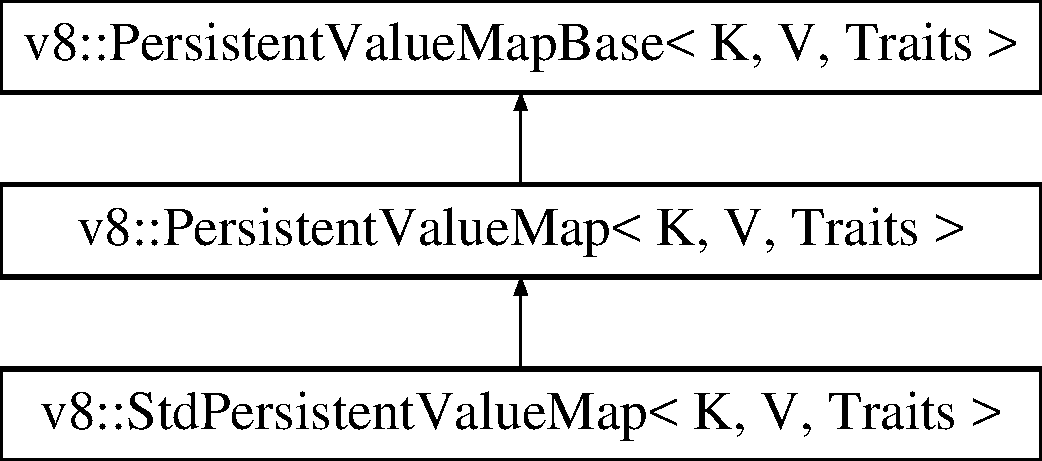
\includegraphics[height=2.000000cm]{classv8_1_1PersistentValueMap}
\end{center}
\end{figure}
\subsection*{Data Structures}
\begin{DoxyCompactItemize}
\item 
class \hyperlink{classv8_1_1PersistentValueMap_1_1PersistentValueReference}{Persistent\+Value\+Reference}
\end{DoxyCompactItemize}
\subsection*{Public Member Functions}
\begin{DoxyCompactItemize}
\item 
\hypertarget{classv8_1_1PersistentValueMap_af8000a75ef84fa719724dc4dadc1e5ee}{}{\bfseries Persistent\+Value\+Map} (\hyperlink{classv8_1_1Isolate}{Isolate} $\ast$isolate)\label{classv8_1_1PersistentValueMap_af8000a75ef84fa719724dc4dadc1e5ee}

\item 
\hypertarget{classv8_1_1PersistentValueMap_ababf27aecff22e0878951f5a6dc44c75}{}\hyperlink{classv8_1_1Isolate}{Isolate} $\ast$ {\bfseries Get\+Isolate} ()\label{classv8_1_1PersistentValueMap_ababf27aecff22e0878951f5a6dc44c75}

\item 
size\+\_\+t \hyperlink{classv8_1_1PersistentValueMap_a01a7f3adb0631e16fcd5d7a1a36e7c0f}{Size} ()
\item 
bool \hyperlink{classv8_1_1PersistentValueMap_a26bb44c09b5356e1b174badf4b2f08e1}{Is\+Weak} ()
\item 
\hyperlink{classv8_1_1Local}{Local}$<$ V $>$ \hyperlink{classv8_1_1PersistentValueMap_a1a09e4ab271a5a68e3a8d01691bd79cb}{Get} (const K \&key)
\item 
bool \hyperlink{classv8_1_1PersistentValueMap_a35a111acbb12de4caf88ed80830aef99}{Contains} (const K \&key)
\item 
bool \hyperlink{classv8_1_1PersistentValueMap_a4c1724c3ac3705e6bacbf0260040e28c}{Set\+Return\+Value} (const K \&key, \hyperlink{classv8_1_1ReturnValue}{Return\+Value}$<$ \hyperlink{classv8_1_1Value}{Value} $>$ return\+Value)
\item 
void \hyperlink{classv8_1_1PersistentValueMap_a27ed125a3114a342305a831a01a426c6}{Set\+Reference} (const K \&key, const \hyperlink{classv8_1_1Persistent}{Persistent}$<$ \hyperlink{classv8_1_1Object}{Object} $>$ \&parent)
\item 
\hyperlink{classv8_1_1UniquePersistent}{Unique\+Persistent}$<$ V $>$ \hyperlink{classv8_1_1PersistentValueMap_af1b5e39f5d0275d8d58d787de5a181d9}{Set} (const K \&key, \hyperlink{classv8_1_1Local}{Local}$<$ V $>$ value)
\item 
\hyperlink{classv8_1_1UniquePersistent}{Unique\+Persistent}$<$ V $>$ \hyperlink{classv8_1_1PersistentValueMap_a31f69108cbb1b481ca5112c22c274681}{Set} (const K \&key, \hyperlink{classv8_1_1UniquePersistent}{Unique\+Persistent}$<$ V $>$ value)
\item 
\hyperlink{classv8_1_1UniquePersistent}{Unique\+Persistent}$<$ V $>$ \hyperlink{classv8_1_1PersistentValueMap_a36df32e99bd89edaa3b28bb573b19c3e}{Remove} (const K \&key)
\item 
void \hyperlink{classv8_1_1PersistentValueMap_acb73f2a873f69adfd15a262ecd90b037}{Clear} ()
\item 
\hyperlink{classv8_1_1PersistentValueMap_1_1PersistentValueReference}{Persistent\+Value\+Reference} \hyperlink{classv8_1_1PersistentValueMap_a541cef25add45efef0586a258eeed1e3}{Get\+Reference} (const K \&key)
\item 
\hyperlink{classv8_1_1UniquePersistent}{Unique\+Persistent}$<$ V $>$ \hyperlink{classv8_1_1PersistentValueMap_a4a6ea22cb9a1adbf52e14f92e6370693}{Set} (const K \&key, \hyperlink{classv8_1_1UniquePersistent}{Unique\+Persistent}$<$ V $>$ value, \hyperlink{classv8_1_1PersistentValueMap_1_1PersistentValueReference}{Persistent\+Value\+Reference} $\ast$reference)
\end{DoxyCompactItemize}


\subsection{Detailed Description}
\subsubsection*{template$<$typename K, typename V, typename Traits$>$class v8\+::\+Persistent\+Value\+Map$<$ K, V, Traits $>$}

A map wrapper that allows using \hyperlink{classv8_1_1UniquePersistent}{Unique\+Persistent} as a mapped value. C++11 embedders don\textquotesingle{}t need this class, as they can use \hyperlink{classv8_1_1UniquePersistent}{Unique\+Persistent} directly in std containers.

The map relies on a backing map, whose type and accessors are described by the Traits class. The backing map will handle values of type Persistent\+Container\+Value, with all conversion into and out of \hyperlink{classv8_1_1V8}{V8} handles being transparently handled by this class. 

\subsection{Member Function Documentation}
\hypertarget{classv8_1_1PersistentValueMap_acb73f2a873f69adfd15a262ecd90b037}{}\index{v8\+::\+Persistent\+Value\+Map@{v8\+::\+Persistent\+Value\+Map}!Clear@{Clear}}
\index{Clear@{Clear}!v8\+::\+Persistent\+Value\+Map@{v8\+::\+Persistent\+Value\+Map}}
\subsubsection[{Clear}]{\setlength{\rightskip}{0pt plus 5cm}template$<$typename K , typename V , typename Traits $>$ void {\bf v8\+::\+Persistent\+Value\+Map}$<$ K, V, Traits $>$\+::Clear (
\begin{DoxyParamCaption}
{}
\end{DoxyParamCaption}
)\hspace{0.3cm}{\ttfamily [inline]}}\label{classv8_1_1PersistentValueMap_acb73f2a873f69adfd15a262ecd90b037}
Traverses the map repeatedly, in case side effects of disposal cause insertions. \hypertarget{classv8_1_1PersistentValueMap_a35a111acbb12de4caf88ed80830aef99}{}\index{v8\+::\+Persistent\+Value\+Map@{v8\+::\+Persistent\+Value\+Map}!Contains@{Contains}}
\index{Contains@{Contains}!v8\+::\+Persistent\+Value\+Map@{v8\+::\+Persistent\+Value\+Map}}
\subsubsection[{Contains}]{\setlength{\rightskip}{0pt plus 5cm}template$<$typename K , typename V , typename Traits $>$ bool {\bf v8\+::\+Persistent\+Value\+Map}$<$ K, V, Traits $>$\+::Contains (
\begin{DoxyParamCaption}
\item[{const K \&}]{key}
\end{DoxyParamCaption}
)\hspace{0.3cm}{\ttfamily [inline]}}\label{classv8_1_1PersistentValueMap_a35a111acbb12de4caf88ed80830aef99}
Check whether a value is contained in the map. \hypertarget{classv8_1_1PersistentValueMap_a1a09e4ab271a5a68e3a8d01691bd79cb}{}\index{v8\+::\+Persistent\+Value\+Map@{v8\+::\+Persistent\+Value\+Map}!Get@{Get}}
\index{Get@{Get}!v8\+::\+Persistent\+Value\+Map@{v8\+::\+Persistent\+Value\+Map}}
\subsubsection[{Get}]{\setlength{\rightskip}{0pt plus 5cm}template$<$typename K , typename V , typename Traits $>$ {\bf Local}$<$V$>$ {\bf v8\+::\+Persistent\+Value\+Map}$<$ K, V, Traits $>$\+::Get (
\begin{DoxyParamCaption}
\item[{const K \&}]{key}
\end{DoxyParamCaption}
)\hspace{0.3cm}{\ttfamily [inline]}}\label{classv8_1_1PersistentValueMap_a1a09e4ab271a5a68e3a8d01691bd79cb}
Get value stored in map. \hypertarget{classv8_1_1PersistentValueMap_a541cef25add45efef0586a258eeed1e3}{}\index{v8\+::\+Persistent\+Value\+Map@{v8\+::\+Persistent\+Value\+Map}!Get\+Reference@{Get\+Reference}}
\index{Get\+Reference@{Get\+Reference}!v8\+::\+Persistent\+Value\+Map@{v8\+::\+Persistent\+Value\+Map}}
\subsubsection[{Get\+Reference}]{\setlength{\rightskip}{0pt plus 5cm}template$<$typename K , typename V , typename Traits $>$ {\bf Persistent\+Value\+Reference} {\bf v8\+::\+Persistent\+Value\+Map}$<$ K, V, Traits $>$\+::Get\+Reference (
\begin{DoxyParamCaption}
\item[{const K \&}]{key}
\end{DoxyParamCaption}
)\hspace{0.3cm}{\ttfamily [inline]}}\label{classv8_1_1PersistentValueMap_a541cef25add45efef0586a258eeed1e3}
Get a reference to a map value. This enables fast, repeated access to a value stored in the map while the map remains unchanged.

Careful\+: This is potentially unsafe, so please use with care. The value will become invalid if the value for this key changes in the underlying map, as a result of Set or Remove for the same key; as a result of the weak callback for the same key; or as a result of calling \hyperlink{classv8_1_1PersistentValueMap_acb73f2a873f69adfd15a262ecd90b037}{Clear()} or destruction of the map. \hypertarget{classv8_1_1PersistentValueMap_a26bb44c09b5356e1b174badf4b2f08e1}{}\index{v8\+::\+Persistent\+Value\+Map@{v8\+::\+Persistent\+Value\+Map}!Is\+Weak@{Is\+Weak}}
\index{Is\+Weak@{Is\+Weak}!v8\+::\+Persistent\+Value\+Map@{v8\+::\+Persistent\+Value\+Map}}
\subsubsection[{Is\+Weak}]{\setlength{\rightskip}{0pt plus 5cm}template$<$typename K , typename V , typename Traits $>$ bool {\bf v8\+::\+Persistent\+Value\+Map}$<$ K, V, Traits $>$\+::Is\+Weak (
\begin{DoxyParamCaption}
{}
\end{DoxyParamCaption}
)\hspace{0.3cm}{\ttfamily [inline]}}\label{classv8_1_1PersistentValueMap_a26bb44c09b5356e1b174badf4b2f08e1}
Return whether the map holds weak persistents. \hypertarget{classv8_1_1PersistentValueMap_a36df32e99bd89edaa3b28bb573b19c3e}{}\index{v8\+::\+Persistent\+Value\+Map@{v8\+::\+Persistent\+Value\+Map}!Remove@{Remove}}
\index{Remove@{Remove}!v8\+::\+Persistent\+Value\+Map@{v8\+::\+Persistent\+Value\+Map}}
\subsubsection[{Remove}]{\setlength{\rightskip}{0pt plus 5cm}template$<$typename K , typename V , typename Traits $>$ {\bf Unique\+Persistent}$<$V$>$ {\bf v8\+::\+Persistent\+Value\+Map}$<$ K, V, Traits $>$\+::Remove (
\begin{DoxyParamCaption}
\item[{const K \&}]{key}
\end{DoxyParamCaption}
)\hspace{0.3cm}{\ttfamily [inline]}}\label{classv8_1_1PersistentValueMap_a36df32e99bd89edaa3b28bb573b19c3e}
Return value for key and remove it from the map. \hypertarget{classv8_1_1PersistentValueMap_af1b5e39f5d0275d8d58d787de5a181d9}{}\index{v8\+::\+Persistent\+Value\+Map@{v8\+::\+Persistent\+Value\+Map}!Set@{Set}}
\index{Set@{Set}!v8\+::\+Persistent\+Value\+Map@{v8\+::\+Persistent\+Value\+Map}}
\subsubsection[{Set}]{\setlength{\rightskip}{0pt plus 5cm}template$<$typename K , typename V , typename Traits $>$ {\bf Unique\+Persistent}$<$V$>$ {\bf v8\+::\+Persistent\+Value\+Map}$<$ K, V, Traits $>$\+::Set (
\begin{DoxyParamCaption}
\item[{const K \&}]{key, }
\item[{{\bf Local}$<$ V $>$}]{value}
\end{DoxyParamCaption}
)\hspace{0.3cm}{\ttfamily [inline]}}\label{classv8_1_1PersistentValueMap_af1b5e39f5d0275d8d58d787de5a181d9}
Put value into map. Depending on Traits\+::k\+Is\+Weak, the value will be held by the map strongly or weakly. Returns old value as \hyperlink{classv8_1_1UniquePersistent}{Unique\+Persistent}. \hypertarget{classv8_1_1PersistentValueMap_a31f69108cbb1b481ca5112c22c274681}{}\index{v8\+::\+Persistent\+Value\+Map@{v8\+::\+Persistent\+Value\+Map}!Set@{Set}}
\index{Set@{Set}!v8\+::\+Persistent\+Value\+Map@{v8\+::\+Persistent\+Value\+Map}}
\subsubsection[{Set}]{\setlength{\rightskip}{0pt plus 5cm}template$<$typename K , typename V , typename Traits $>$ {\bf Unique\+Persistent}$<$V$>$ {\bf v8\+::\+Persistent\+Value\+Map}$<$ K, V, Traits $>$\+::Set (
\begin{DoxyParamCaption}
\item[{const K \&}]{key, }
\item[{{\bf Unique\+Persistent}$<$ V $>$}]{value}
\end{DoxyParamCaption}
)\hspace{0.3cm}{\ttfamily [inline]}}\label{classv8_1_1PersistentValueMap_a31f69108cbb1b481ca5112c22c274681}
Put value into map, like \hyperlink{classv8_1_1PersistentValueMap_af1b5e39f5d0275d8d58d787de5a181d9}{Set(const K\&, Local$<$\+V$>$)}. \hypertarget{classv8_1_1PersistentValueMap_a4a6ea22cb9a1adbf52e14f92e6370693}{}\index{v8\+::\+Persistent\+Value\+Map@{v8\+::\+Persistent\+Value\+Map}!Set@{Set}}
\index{Set@{Set}!v8\+::\+Persistent\+Value\+Map@{v8\+::\+Persistent\+Value\+Map}}
\subsubsection[{Set}]{\setlength{\rightskip}{0pt plus 5cm}template$<$typename K , typename V , typename Traits $>$ {\bf Unique\+Persistent}$<$V$>$ {\bf v8\+::\+Persistent\+Value\+Map}$<$ K, V, Traits $>$\+::Set (
\begin{DoxyParamCaption}
\item[{const K \&}]{key, }
\item[{{\bf Unique\+Persistent}$<$ V $>$}]{value, }
\item[{{\bf Persistent\+Value\+Reference} $\ast$}]{reference}
\end{DoxyParamCaption}
)\hspace{0.3cm}{\ttfamily [inline]}}\label{classv8_1_1PersistentValueMap_a4a6ea22cb9a1adbf52e14f92e6370693}
Put a value into the map and update the reference. Restrictions of Get\+Reference apply here as well. \hypertarget{classv8_1_1PersistentValueMap_a27ed125a3114a342305a831a01a426c6}{}\index{v8\+::\+Persistent\+Value\+Map@{v8\+::\+Persistent\+Value\+Map}!Set\+Reference@{Set\+Reference}}
\index{Set\+Reference@{Set\+Reference}!v8\+::\+Persistent\+Value\+Map@{v8\+::\+Persistent\+Value\+Map}}
\subsubsection[{Set\+Reference}]{\setlength{\rightskip}{0pt plus 5cm}template$<$typename K , typename V , typename Traits $>$ void {\bf v8\+::\+Persistent\+Value\+Map}$<$ K, V, Traits $>$\+::Set\+Reference (
\begin{DoxyParamCaption}
\item[{const K \&}]{key, }
\item[{const {\bf Persistent}$<$ {\bf Object} $>$ \&}]{parent}
\end{DoxyParamCaption}
)\hspace{0.3cm}{\ttfamily [inline]}}\label{classv8_1_1PersistentValueMap_a27ed125a3114a342305a831a01a426c6}
Call \hyperlink{classv8_1_1Isolate_a055fc73d18747b96c51f00599cdd3ec1}{Isolate\+::\+Set\+Reference} with the given parent and the map value. \hypertarget{classv8_1_1PersistentValueMap_a4c1724c3ac3705e6bacbf0260040e28c}{}\index{v8\+::\+Persistent\+Value\+Map@{v8\+::\+Persistent\+Value\+Map}!Set\+Return\+Value@{Set\+Return\+Value}}
\index{Set\+Return\+Value@{Set\+Return\+Value}!v8\+::\+Persistent\+Value\+Map@{v8\+::\+Persistent\+Value\+Map}}
\subsubsection[{Set\+Return\+Value}]{\setlength{\rightskip}{0pt plus 5cm}template$<$typename K , typename V , typename Traits $>$ bool {\bf v8\+::\+Persistent\+Value\+Map}$<$ K, V, Traits $>$\+::Set\+Return\+Value (
\begin{DoxyParamCaption}
\item[{const K \&}]{key, }
\item[{{\bf Return\+Value}$<$ {\bf Value} $>$}]{return\+Value}
\end{DoxyParamCaption}
)\hspace{0.3cm}{\ttfamily [inline]}}\label{classv8_1_1PersistentValueMap_a4c1724c3ac3705e6bacbf0260040e28c}
Get value stored in map and set it in return\+Value. Return true if a value was found. \hypertarget{classv8_1_1PersistentValueMap_a01a7f3adb0631e16fcd5d7a1a36e7c0f}{}\index{v8\+::\+Persistent\+Value\+Map@{v8\+::\+Persistent\+Value\+Map}!Size@{Size}}
\index{Size@{Size}!v8\+::\+Persistent\+Value\+Map@{v8\+::\+Persistent\+Value\+Map}}
\subsubsection[{Size}]{\setlength{\rightskip}{0pt plus 5cm}template$<$typename K , typename V , typename Traits $>$ size\+\_\+t {\bf v8\+::\+Persistent\+Value\+Map}$<$ K, V, Traits $>$\+::Size (
\begin{DoxyParamCaption}
{}
\end{DoxyParamCaption}
)\hspace{0.3cm}{\ttfamily [inline]}}\label{classv8_1_1PersistentValueMap_a01a7f3adb0631e16fcd5d7a1a36e7c0f}
Return size of the map. 

The documentation for this class was generated from the following file\+:\begin{DoxyCompactItemize}
\item 
v8/include/v8-\/util.\+h\end{DoxyCompactItemize}

\hypertarget{classv8_1_1PersistentValueMapBase}{}\section{v8\+:\+:Persistent\+Value\+Map\+Base$<$ K, V, Traits $>$ Class Template Reference}
\label{classv8_1_1PersistentValueMapBase}\index{v8\+::\+Persistent\+Value\+Map\+Base$<$ K, V, Traits $>$@{v8\+::\+Persistent\+Value\+Map\+Base$<$ K, V, Traits $>$}}


{\ttfamily \#include $<$v8-\/util.\+h$>$}

Inheritance diagram for v8\+:\+:Persistent\+Value\+Map\+Base$<$ K, V, Traits $>$\+:\begin{figure}[H]
\begin{center}
\leavevmode
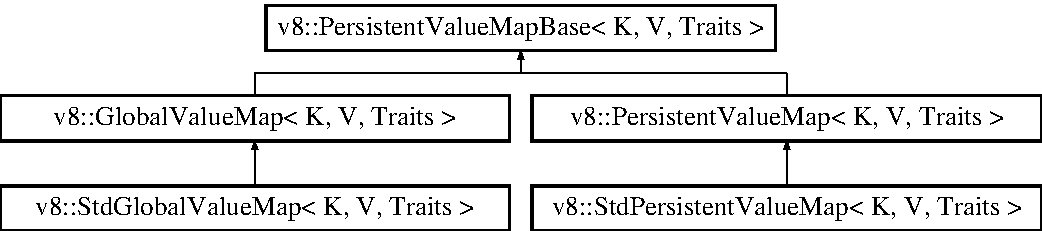
\includegraphics[height=3.000000cm]{classv8_1_1PersistentValueMapBase}
\end{center}
\end{figure}
\subsection*{Data Structures}
\begin{DoxyCompactItemize}
\item 
class \hyperlink{classv8_1_1PersistentValueMapBase_1_1PersistentValueReference}{Persistent\+Value\+Reference}
\end{DoxyCompactItemize}
\subsection*{Public Member Functions}
\begin{DoxyCompactItemize}
\item 
\hyperlink{classv8_1_1Isolate}{Isolate} $\ast$ {\bfseries Get\+Isolate} ()\hypertarget{classv8_1_1PersistentValueMapBase_a80da7adc6e8bdb166912075346116978}{}\label{classv8_1_1PersistentValueMapBase_a80da7adc6e8bdb166912075346116978}

\item 
size\+\_\+t \hyperlink{classv8_1_1PersistentValueMapBase_ade5c5db2a968fdabe073649e85b837eb}{Size} ()
\item 
bool \hyperlink{classv8_1_1PersistentValueMapBase_a9f824b13dd30605589508db2740dd678}{Is\+Weak} ()
\item 
\hyperlink{classv8_1_1Local}{Local}$<$ V $>$ \hyperlink{classv8_1_1PersistentValueMapBase_a16b8f906ea42036c2f37d44813bf2a72}{Get} (const K \&key)
\item 
bool \hyperlink{classv8_1_1PersistentValueMapBase_a8c68e5f99c4042541c6d32232c97282a}{Contains} (const K \&key)
\item 
bool \hyperlink{classv8_1_1PersistentValueMapBase_a85201649d2bbd0ffdebe8be3d5c6447a}{Set\+Return\+Value} (const K \&key, \hyperlink{classv8_1_1ReturnValue}{Return\+Value}$<$ \hyperlink{classv8_1_1Value}{Value} $>$ return\+Value)
\item 
void \hyperlink{classv8_1_1PersistentValueMapBase_a6fa5f720b283dd9fa626a67e7687dcd0}{Set\+Reference} (const K \&key, const \hyperlink{classv8_1_1Persistent}{Persistent}$<$ \hyperlink{classv8_1_1Object}{Object} $>$ \&parent)
\item 
void \hyperlink{classv8_1_1PersistentValueMapBase_a7d1cd63172b997dfaac9d0f009edd709}{Register\+Externally\+Referenced\+Object} (K \&key)
\item 
\hyperlink{classv8_1_1Global}{Global}$<$ V $>$ \hyperlink{classv8_1_1PersistentValueMapBase_abd75a4c050416712167ba0bb9eace097}{Remove} (const K \&key)
\item 
void \hyperlink{classv8_1_1PersistentValueMapBase_a1bf074e7a7c24713c9a3d40ddce89e74}{Clear} ()
\item 
\hyperlink{classv8_1_1PersistentValueMapBase_1_1PersistentValueReference}{Persistent\+Value\+Reference} \hyperlink{classv8_1_1PersistentValueMapBase_a52e74c69b94c7ce77a65af9f32d68af4}{Get\+Reference} (const K \&key)
\end{DoxyCompactItemize}
\subsection*{Protected Member Functions}
\begin{DoxyCompactItemize}
\item 
{\bfseries Persistent\+Value\+Map\+Base} (\hyperlink{classv8_1_1Isolate}{Isolate} $\ast$isolate)\hypertarget{classv8_1_1PersistentValueMapBase_a1adee3f8b1ff929f07ddf9e94c6108ed}{}\label{classv8_1_1PersistentValueMapBase_a1adee3f8b1ff929f07ddf9e94c6108ed}

\item 
\hyperlink{classv8_1_1Isolate}{Isolate} $\ast$ {\bfseries isolate} ()\hypertarget{classv8_1_1PersistentValueMapBase_af2e83791955c6027213dd979eebeb8f4}{}\label{classv8_1_1PersistentValueMapBase_af2e83791955c6027213dd979eebeb8f4}

\item 
Traits\+::\+Impl $\ast$ {\bfseries impl} ()\hypertarget{classv8_1_1PersistentValueMapBase_aacd576258fbffaf366436a6ecdd8cdf5}{}\label{classv8_1_1PersistentValueMapBase_aacd576258fbffaf366436a6ecdd8cdf5}

\item 
void {\bfseries Remove\+Weak} (const K \&key)\hypertarget{classv8_1_1PersistentValueMapBase_a5c16ace49c257f760c92a010a93b4884}{}\label{classv8_1_1PersistentValueMapBase_a5c16ace49c257f760c92a010a93b4884}

\end{DoxyCompactItemize}
\subsection*{Static Protected Member Functions}
\begin{DoxyCompactItemize}
\item 
static V $\ast$ {\bfseries From\+Val} (Persistent\+Container\+Value v)\hypertarget{classv8_1_1PersistentValueMapBase_af8fcd471f2d53ffca9881f7c436044e8}{}\label{classv8_1_1PersistentValueMapBase_af8fcd471f2d53ffca9881f7c436044e8}

\item 
static Persistent\+Container\+Value {\bfseries Clear\+And\+Leak} (\hyperlink{classv8_1_1Global}{Global}$<$ V $>$ $\ast$persistent)\hypertarget{classv8_1_1PersistentValueMapBase_a7b083c75829bbc4177729ffe9827c4ac}{}\label{classv8_1_1PersistentValueMapBase_a7b083c75829bbc4177729ffe9827c4ac}

\item 
static Persistent\+Container\+Value {\bfseries Leak} (\hyperlink{classv8_1_1Global}{Global}$<$ V $>$ $\ast$persistent)\hypertarget{classv8_1_1PersistentValueMapBase_adacf68ca7b9fb19deab68711a70a8313}{}\label{classv8_1_1PersistentValueMapBase_adacf68ca7b9fb19deab68711a70a8313}

\item 
static \hyperlink{classv8_1_1Global}{Global}$<$ V $>$ \hyperlink{classv8_1_1PersistentValueMapBase_a9ffa7a4e0c59121c0471d71c04112966}{Release} (Persistent\+Container\+Value v)
\end{DoxyCompactItemize}


\subsection{Detailed Description}
\subsubsection*{template$<$typename K, typename V, typename Traits$>$\\*
class v8\+::\+Persistent\+Value\+Map\+Base$<$ K, V, Traits $>$}

A map wrapper that allows using \hyperlink{classv8_1_1Global}{Global} as a mapped value. C++11 embedders don\textquotesingle{}t need this class, as they can use \hyperlink{classv8_1_1Global}{Global} directly in std containers.

The map relies on a backing map, whose type and accessors are described by the Traits class. The backing map will handle values of type Persistent\+Container\+Value, with all conversion into and out of \hyperlink{classv8_1_1V8}{V8} handles being transparently handled by this class. 

\subsection{Member Function Documentation}
\index{v8\+::\+Persistent\+Value\+Map\+Base@{v8\+::\+Persistent\+Value\+Map\+Base}!Clear@{Clear}}
\index{Clear@{Clear}!v8\+::\+Persistent\+Value\+Map\+Base@{v8\+::\+Persistent\+Value\+Map\+Base}}
\subsubsection[{\texorpdfstring{Clear()}{Clear()}}]{\setlength{\rightskip}{0pt plus 5cm}template$<$typename K , typename V , typename Traits $>$ void {\bf v8\+::\+Persistent\+Value\+Map\+Base}$<$ K, V, Traits $>$\+::Clear (
\begin{DoxyParamCaption}
{}
\end{DoxyParamCaption}
)\hspace{0.3cm}{\ttfamily [inline]}}\hypertarget{classv8_1_1PersistentValueMapBase_a1bf074e7a7c24713c9a3d40ddce89e74}{}\label{classv8_1_1PersistentValueMapBase_a1bf074e7a7c24713c9a3d40ddce89e74}
Traverses the map repeatedly, in case side effects of disposal cause insertions. \index{v8\+::\+Persistent\+Value\+Map\+Base@{v8\+::\+Persistent\+Value\+Map\+Base}!Contains@{Contains}}
\index{Contains@{Contains}!v8\+::\+Persistent\+Value\+Map\+Base@{v8\+::\+Persistent\+Value\+Map\+Base}}
\subsubsection[{\texorpdfstring{Contains(const K \&key)}{Contains(const K &key)}}]{\setlength{\rightskip}{0pt plus 5cm}template$<$typename K , typename V , typename Traits $>$ bool {\bf v8\+::\+Persistent\+Value\+Map\+Base}$<$ K, V, Traits $>$\+::Contains (
\begin{DoxyParamCaption}
\item[{const K \&}]{key}
\end{DoxyParamCaption}
)\hspace{0.3cm}{\ttfamily [inline]}}\hypertarget{classv8_1_1PersistentValueMapBase_a8c68e5f99c4042541c6d32232c97282a}{}\label{classv8_1_1PersistentValueMapBase_a8c68e5f99c4042541c6d32232c97282a}
Check whether a value is contained in the map. \index{v8\+::\+Persistent\+Value\+Map\+Base@{v8\+::\+Persistent\+Value\+Map\+Base}!Get@{Get}}
\index{Get@{Get}!v8\+::\+Persistent\+Value\+Map\+Base@{v8\+::\+Persistent\+Value\+Map\+Base}}
\subsubsection[{\texorpdfstring{Get(const K \&key)}{Get(const K &key)}}]{\setlength{\rightskip}{0pt plus 5cm}template$<$typename K , typename V , typename Traits $>$ {\bf Local}$<$V$>$ {\bf v8\+::\+Persistent\+Value\+Map\+Base}$<$ K, V, Traits $>$\+::Get (
\begin{DoxyParamCaption}
\item[{const K \&}]{key}
\end{DoxyParamCaption}
)\hspace{0.3cm}{\ttfamily [inline]}}\hypertarget{classv8_1_1PersistentValueMapBase_a16b8f906ea42036c2f37d44813bf2a72}{}\label{classv8_1_1PersistentValueMapBase_a16b8f906ea42036c2f37d44813bf2a72}
Get value stored in map. \index{v8\+::\+Persistent\+Value\+Map\+Base@{v8\+::\+Persistent\+Value\+Map\+Base}!Get\+Reference@{Get\+Reference}}
\index{Get\+Reference@{Get\+Reference}!v8\+::\+Persistent\+Value\+Map\+Base@{v8\+::\+Persistent\+Value\+Map\+Base}}
\subsubsection[{\texorpdfstring{Get\+Reference(const K \&key)}{GetReference(const K &key)}}]{\setlength{\rightskip}{0pt plus 5cm}template$<$typename K , typename V , typename Traits $>$ {\bf Persistent\+Value\+Reference} {\bf v8\+::\+Persistent\+Value\+Map\+Base}$<$ K, V, Traits $>$\+::Get\+Reference (
\begin{DoxyParamCaption}
\item[{const K \&}]{key}
\end{DoxyParamCaption}
)\hspace{0.3cm}{\ttfamily [inline]}}\hypertarget{classv8_1_1PersistentValueMapBase_a52e74c69b94c7ce77a65af9f32d68af4}{}\label{classv8_1_1PersistentValueMapBase_a52e74c69b94c7ce77a65af9f32d68af4}
Get a reference to a map value. This enables fast, repeated access to a value stored in the map while the map remains unchanged.

Careful\+: This is potentially unsafe, so please use with care. The value will become invalid if the value for this key changes in the underlying map, as a result of \hyperlink{classv8_1_1Set}{Set} or Remove for the same key; as a result of the weak callback for the same key; or as a result of calling \hyperlink{classv8_1_1PersistentValueMapBase_a1bf074e7a7c24713c9a3d40ddce89e74}{Clear()} or destruction of the map. \index{v8\+::\+Persistent\+Value\+Map\+Base@{v8\+::\+Persistent\+Value\+Map\+Base}!Is\+Weak@{Is\+Weak}}
\index{Is\+Weak@{Is\+Weak}!v8\+::\+Persistent\+Value\+Map\+Base@{v8\+::\+Persistent\+Value\+Map\+Base}}
\subsubsection[{\texorpdfstring{Is\+Weak()}{IsWeak()}}]{\setlength{\rightskip}{0pt plus 5cm}template$<$typename K , typename V , typename Traits $>$ bool {\bf v8\+::\+Persistent\+Value\+Map\+Base}$<$ K, V, Traits $>$\+::Is\+Weak (
\begin{DoxyParamCaption}
{}
\end{DoxyParamCaption}
)\hspace{0.3cm}{\ttfamily [inline]}}\hypertarget{classv8_1_1PersistentValueMapBase_a9f824b13dd30605589508db2740dd678}{}\label{classv8_1_1PersistentValueMapBase_a9f824b13dd30605589508db2740dd678}
Return whether the map holds weak persistents. \index{v8\+::\+Persistent\+Value\+Map\+Base@{v8\+::\+Persistent\+Value\+Map\+Base}!Register\+Externally\+Referenced\+Object@{Register\+Externally\+Referenced\+Object}}
\index{Register\+Externally\+Referenced\+Object@{Register\+Externally\+Referenced\+Object}!v8\+::\+Persistent\+Value\+Map\+Base@{v8\+::\+Persistent\+Value\+Map\+Base}}
\subsubsection[{\texorpdfstring{Register\+Externally\+Referenced\+Object(\+K \&key)}{RegisterExternallyReferencedObject(K &key)}}]{\setlength{\rightskip}{0pt plus 5cm}template$<$typename K , typename V , typename Traits $>$ void {\bf v8\+::\+Persistent\+Value\+Map\+Base}$<$ K, V, Traits $>$\+::Register\+Externally\+Referenced\+Object (
\begin{DoxyParamCaption}
\item[{K \&}]{key}
\end{DoxyParamCaption}
)\hspace{0.3cm}{\ttfamily [inline]}}\hypertarget{classv8_1_1PersistentValueMapBase_a7d1cd63172b997dfaac9d0f009edd709}{}\label{classv8_1_1PersistentValueMapBase_a7d1cd63172b997dfaac9d0f009edd709}
Call V8\+::\+Register\+Externally\+Referenced\+Object with the map value for given key. \index{v8\+::\+Persistent\+Value\+Map\+Base@{v8\+::\+Persistent\+Value\+Map\+Base}!Release@{Release}}
\index{Release@{Release}!v8\+::\+Persistent\+Value\+Map\+Base@{v8\+::\+Persistent\+Value\+Map\+Base}}
\subsubsection[{\texorpdfstring{Release(\+Persistent\+Container\+Value v)}{Release(PersistentContainerValue v)}}]{\setlength{\rightskip}{0pt plus 5cm}template$<$typename K , typename V , typename Traits $>$ static {\bf Global}$<$V$>$ {\bf v8\+::\+Persistent\+Value\+Map\+Base}$<$ K, V, Traits $>$\+::Release (
\begin{DoxyParamCaption}
\item[{Persistent\+Container\+Value}]{v}
\end{DoxyParamCaption}
)\hspace{0.3cm}{\ttfamily [inline]}, {\ttfamily [static]}, {\ttfamily [protected]}}\hypertarget{classv8_1_1PersistentValueMapBase_a9ffa7a4e0c59121c0471d71c04112966}{}\label{classv8_1_1PersistentValueMapBase_a9ffa7a4e0c59121c0471d71c04112966}
Return a container value as \hyperlink{classv8_1_1Global}{Global} and make sure the weak callback is properly disposed of. All remove functionality should go through this. \index{v8\+::\+Persistent\+Value\+Map\+Base@{v8\+::\+Persistent\+Value\+Map\+Base}!Remove@{Remove}}
\index{Remove@{Remove}!v8\+::\+Persistent\+Value\+Map\+Base@{v8\+::\+Persistent\+Value\+Map\+Base}}
\subsubsection[{\texorpdfstring{Remove(const K \&key)}{Remove(const K &key)}}]{\setlength{\rightskip}{0pt plus 5cm}template$<$typename K , typename V , typename Traits $>$ {\bf Global}$<$V$>$ {\bf v8\+::\+Persistent\+Value\+Map\+Base}$<$ K, V, Traits $>$\+::Remove (
\begin{DoxyParamCaption}
\item[{const K \&}]{key}
\end{DoxyParamCaption}
)\hspace{0.3cm}{\ttfamily [inline]}}\hypertarget{classv8_1_1PersistentValueMapBase_abd75a4c050416712167ba0bb9eace097}{}\label{classv8_1_1PersistentValueMapBase_abd75a4c050416712167ba0bb9eace097}
Return value for key and remove it from the map. \index{v8\+::\+Persistent\+Value\+Map\+Base@{v8\+::\+Persistent\+Value\+Map\+Base}!Set\+Reference@{Set\+Reference}}
\index{Set\+Reference@{Set\+Reference}!v8\+::\+Persistent\+Value\+Map\+Base@{v8\+::\+Persistent\+Value\+Map\+Base}}
\subsubsection[{\texorpdfstring{Set\+Reference(const K \&key, const Persistent$<$ Object $>$ \&parent)}{SetReference(const K &key, const Persistent< Object > &parent)}}]{\setlength{\rightskip}{0pt plus 5cm}template$<$typename K , typename V , typename Traits $>$ void {\bf v8\+::\+Persistent\+Value\+Map\+Base}$<$ K, V, Traits $>$\+::Set\+Reference (
\begin{DoxyParamCaption}
\item[{const K \&}]{key, }
\item[{const {\bf Persistent}$<$ {\bf Object} $>$ \&}]{parent}
\end{DoxyParamCaption}
)\hspace{0.3cm}{\ttfamily [inline]}}\hypertarget{classv8_1_1PersistentValueMapBase_a6fa5f720b283dd9fa626a67e7687dcd0}{}\label{classv8_1_1PersistentValueMapBase_a6fa5f720b283dd9fa626a67e7687dcd0}
Call \hyperlink{classv8_1_1Isolate_a055fc73d18747b96c51f00599cdd3ec1}{Isolate\+::\+Set\+Reference} with the given parent and the map value. \index{v8\+::\+Persistent\+Value\+Map\+Base@{v8\+::\+Persistent\+Value\+Map\+Base}!Set\+Return\+Value@{Set\+Return\+Value}}
\index{Set\+Return\+Value@{Set\+Return\+Value}!v8\+::\+Persistent\+Value\+Map\+Base@{v8\+::\+Persistent\+Value\+Map\+Base}}
\subsubsection[{\texorpdfstring{Set\+Return\+Value(const K \&key, Return\+Value$<$ Value $>$ return\+Value)}{SetReturnValue(const K &key, ReturnValue< Value > returnValue)}}]{\setlength{\rightskip}{0pt plus 5cm}template$<$typename K , typename V , typename Traits $>$ bool {\bf v8\+::\+Persistent\+Value\+Map\+Base}$<$ K, V, Traits $>$\+::Set\+Return\+Value (
\begin{DoxyParamCaption}
\item[{const K \&}]{key, }
\item[{{\bf Return\+Value}$<$ {\bf Value} $>$}]{return\+Value}
\end{DoxyParamCaption}
)\hspace{0.3cm}{\ttfamily [inline]}}\hypertarget{classv8_1_1PersistentValueMapBase_a85201649d2bbd0ffdebe8be3d5c6447a}{}\label{classv8_1_1PersistentValueMapBase_a85201649d2bbd0ffdebe8be3d5c6447a}
Get value stored in map and set it in return\+Value. Return true if a value was found. \index{v8\+::\+Persistent\+Value\+Map\+Base@{v8\+::\+Persistent\+Value\+Map\+Base}!Size@{Size}}
\index{Size@{Size}!v8\+::\+Persistent\+Value\+Map\+Base@{v8\+::\+Persistent\+Value\+Map\+Base}}
\subsubsection[{\texorpdfstring{Size()}{Size()}}]{\setlength{\rightskip}{0pt plus 5cm}template$<$typename K , typename V , typename Traits $>$ size\+\_\+t {\bf v8\+::\+Persistent\+Value\+Map\+Base}$<$ K, V, Traits $>$\+::Size (
\begin{DoxyParamCaption}
{}
\end{DoxyParamCaption}
)\hspace{0.3cm}{\ttfamily [inline]}}\hypertarget{classv8_1_1PersistentValueMapBase_ade5c5db2a968fdabe073649e85b837eb}{}\label{classv8_1_1PersistentValueMapBase_ade5c5db2a968fdabe073649e85b837eb}
Return size of the map. 

The documentation for this class was generated from the following file\+:\begin{DoxyCompactItemize}
\item 
v8/include/v8-\/util.\+h\end{DoxyCompactItemize}

\hypertarget{classv8_1_1PersistentValueMapBase_1_1PersistentValueReference}{}\section{v8\+:\+:Persistent\+Value\+Map\+Base$<$ K, V, Traits $>$\+:\+:Persistent\+Value\+Reference Class Reference}
\label{classv8_1_1PersistentValueMapBase_1_1PersistentValueReference}\index{v8\+::\+Persistent\+Value\+Map\+Base$<$ K, V, Traits $>$\+::\+Persistent\+Value\+Reference@{v8\+::\+Persistent\+Value\+Map\+Base$<$ K, V, Traits $>$\+::\+Persistent\+Value\+Reference}}


{\ttfamily \#include $<$v8-\/util.\+h$>$}

\subsection*{Public Member Functions}
\begin{DoxyCompactItemize}
\item 
{\bfseries Persistent\+Value\+Reference} (const \hyperlink{classv8_1_1PersistentValueMapBase_1_1PersistentValueReference}{Persistent\+Value\+Reference} \&other)\hypertarget{classv8_1_1PersistentValueMapBase_1_1PersistentValueReference_a47103822e6717eb42de116ddc773e334}{}\label{classv8_1_1PersistentValueMapBase_1_1PersistentValueReference_a47103822e6717eb42de116ddc773e334}

\item 
\hyperlink{classv8_1_1Local}{Local}$<$ V $>$ {\bfseries New\+Local} (\hyperlink{classv8_1_1Isolate}{Isolate} $\ast$isolate) const \hypertarget{classv8_1_1PersistentValueMapBase_1_1PersistentValueReference_a714a3ff6ea3e196bdb2ec244adf39e5f}{}\label{classv8_1_1PersistentValueMapBase_1_1PersistentValueReference_a714a3ff6ea3e196bdb2ec244adf39e5f}

\item 
bool {\bfseries Is\+Empty} () const \hypertarget{classv8_1_1PersistentValueMapBase_1_1PersistentValueReference_a39e28fe15080e676039deeaf7a8e57b5}{}\label{classv8_1_1PersistentValueMapBase_1_1PersistentValueReference_a39e28fe15080e676039deeaf7a8e57b5}

\item 
{\footnotesize template$<$typename T $>$ }\\bool {\bfseries Set\+Return\+Value} (\hyperlink{classv8_1_1ReturnValue}{Return\+Value}$<$ T $>$ return\+Value)\hypertarget{classv8_1_1PersistentValueMapBase_1_1PersistentValueReference_a4003b2d7d0f3cc84574d2e74a1713f27}{}\label{classv8_1_1PersistentValueMapBase_1_1PersistentValueReference_a4003b2d7d0f3cc84574d2e74a1713f27}

\item 
void {\bfseries Reset} ()\hypertarget{classv8_1_1PersistentValueMapBase_1_1PersistentValueReference_a94c91d959beb24cad37458b2ae43a97b}{}\label{classv8_1_1PersistentValueMapBase_1_1PersistentValueReference_a94c91d959beb24cad37458b2ae43a97b}

\item 
void {\bfseries operator=} (const \hyperlink{classv8_1_1PersistentValueMapBase_1_1PersistentValueReference}{Persistent\+Value\+Reference} \&other)\hypertarget{classv8_1_1PersistentValueMapBase_1_1PersistentValueReference_abcbf6c9229d0b322c64fe5110726c421}{}\label{classv8_1_1PersistentValueMapBase_1_1PersistentValueReference_abcbf6c9229d0b322c64fe5110726c421}

\end{DoxyCompactItemize}
\subsection*{Friends}
\begin{DoxyCompactItemize}
\item 
class {\bfseries Persistent\+Value\+Map\+Base}\hypertarget{classv8_1_1PersistentValueMapBase_1_1PersistentValueReference_ae5cccd63ef6d94c509ad8b6970d4017d}{}\label{classv8_1_1PersistentValueMapBase_1_1PersistentValueReference_ae5cccd63ef6d94c509ad8b6970d4017d}

\item 
class {\bfseries Persistent\+Value\+Map$<$ K, V, Traits $>$}\hypertarget{classv8_1_1PersistentValueMapBase_1_1PersistentValueReference_a22fcaa9f3ba179f3bb566eda5b93790d}{}\label{classv8_1_1PersistentValueMapBase_1_1PersistentValueReference_a22fcaa9f3ba179f3bb566eda5b93790d}

\item 
class {\bfseries Global\+Value\+Map$<$ K, V, Traits $>$}\hypertarget{classv8_1_1PersistentValueMapBase_1_1PersistentValueReference_a41811cde55d1ef227d1ba28778d95d08}{}\label{classv8_1_1PersistentValueMapBase_1_1PersistentValueReference_a41811cde55d1ef227d1ba28778d95d08}

\end{DoxyCompactItemize}


\subsection{Detailed Description}
\subsubsection*{template$<$typename K, typename V, typename Traits$>$\\*
class v8\+::\+Persistent\+Value\+Map\+Base$<$ K, V, Traits $>$\+::\+Persistent\+Value\+Reference}

Helper class for Get\+Reference/\+Set\+With\+Reference. Do not use outside that context. 

The documentation for this class was generated from the following file\+:\begin{DoxyCompactItemize}
\item 
v8/include/v8-\/util.\+h\end{DoxyCompactItemize}

\hypertarget{classv8_1_1PersistentValueVector}{}\section{v8\+:\+:Persistent\+Value\+Vector$<$ V, Traits $>$ Class Template Reference}
\label{classv8_1_1PersistentValueVector}\index{v8\+::\+Persistent\+Value\+Vector$<$ V, Traits $>$@{v8\+::\+Persistent\+Value\+Vector$<$ V, Traits $>$}}


{\ttfamily \#include $<$v8-\/util.\+h$>$}

\subsection*{Public Member Functions}
\begin{DoxyCompactItemize}
\item 
\hypertarget{classv8_1_1PersistentValueVector_ab6b9994133c30359ad7a02d3cc05219c}{}{\bfseries Persistent\+Value\+Vector} (\hyperlink{classv8_1_1Isolate}{Isolate} $\ast$isolate)\label{classv8_1_1PersistentValueVector_ab6b9994133c30359ad7a02d3cc05219c}

\item 
void \hyperlink{classv8_1_1PersistentValueVector_a02376c6d16be29084db46f65473477fb}{Append} (\hyperlink{classv8_1_1Local}{Local}$<$ V $>$ value)
\item 
void \hyperlink{classv8_1_1PersistentValueVector_aff8a1aca35be80ac9744c5100ae2dae0}{Append} (\hyperlink{classv8_1_1UniquePersistent}{Unique\+Persistent}$<$ V $>$ persistent)
\item 
bool \hyperlink{classv8_1_1PersistentValueVector_a9ad869bc3f60fc227fecf202b36b650a}{Is\+Empty} () const 
\item 
size\+\_\+t \hyperlink{classv8_1_1PersistentValueVector_a0e152d147a2553746e56cbf9e6311506}{Size} () const 
\item 
\hyperlink{classv8_1_1Local}{Local}$<$ V $>$ \hyperlink{classv8_1_1PersistentValueVector_a7b47cacf60ddfa3e2a7f57d788f18b84}{Get} (size\+\_\+t index) const 
\item 
void \hyperlink{classv8_1_1PersistentValueVector_ad07f449c2004b4f3d91e58cabde99a53}{Clear} ()
\item 
void \hyperlink{classv8_1_1PersistentValueVector_ad4cccfee3a275986578276efe0c78510}{Reserve\+Capacity} (size\+\_\+t capacity)
\end{DoxyCompactItemize}


\subsection{Detailed Description}
\subsubsection*{template$<$typename V, typename Traits = Default\+Persistent\+Value\+Vector\+Traits$>$class v8\+::\+Persistent\+Value\+Vector$<$ V, Traits $>$}

A vector wrapper that safely stores \hyperlink{classv8_1_1UniquePersistent}{Unique\+Persistent} values. C++11 embedders don\textquotesingle{}t need this class, as they can use \hyperlink{classv8_1_1UniquePersistent}{Unique\+Persistent} directly in std containers.

This class relies on a backing vector implementation, whose type and methods are described by the Traits class. The backing map will handle values of type Persistent\+Container\+Value, with all conversion into and out of \hyperlink{classv8_1_1V8}{V8} handles being transparently handled by this class. 

\subsection{Member Function Documentation}
\hypertarget{classv8_1_1PersistentValueVector_a02376c6d16be29084db46f65473477fb}{}\index{v8\+::\+Persistent\+Value\+Vector@{v8\+::\+Persistent\+Value\+Vector}!Append@{Append}}
\index{Append@{Append}!v8\+::\+Persistent\+Value\+Vector@{v8\+::\+Persistent\+Value\+Vector}}
\subsubsection[{Append}]{\setlength{\rightskip}{0pt plus 5cm}template$<$typename V , typename Traits  = Default\+Persistent\+Value\+Vector\+Traits$>$ void {\bf v8\+::\+Persistent\+Value\+Vector}$<$ V, Traits $>$\+::Append (
\begin{DoxyParamCaption}
\item[{{\bf Local}$<$ V $>$}]{value}
\end{DoxyParamCaption}
)\hspace{0.3cm}{\ttfamily [inline]}}\label{classv8_1_1PersistentValueVector_a02376c6d16be29084db46f65473477fb}
Append a value to the vector. \hypertarget{classv8_1_1PersistentValueVector_aff8a1aca35be80ac9744c5100ae2dae0}{}\index{v8\+::\+Persistent\+Value\+Vector@{v8\+::\+Persistent\+Value\+Vector}!Append@{Append}}
\index{Append@{Append}!v8\+::\+Persistent\+Value\+Vector@{v8\+::\+Persistent\+Value\+Vector}}
\subsubsection[{Append}]{\setlength{\rightskip}{0pt plus 5cm}template$<$typename V , typename Traits  = Default\+Persistent\+Value\+Vector\+Traits$>$ void {\bf v8\+::\+Persistent\+Value\+Vector}$<$ V, Traits $>$\+::Append (
\begin{DoxyParamCaption}
\item[{{\bf Unique\+Persistent}$<$ V $>$}]{persistent}
\end{DoxyParamCaption}
)\hspace{0.3cm}{\ttfamily [inline]}}\label{classv8_1_1PersistentValueVector_aff8a1aca35be80ac9744c5100ae2dae0}
Append a persistent\textquotesingle{}s value to the vector. \hypertarget{classv8_1_1PersistentValueVector_ad07f449c2004b4f3d91e58cabde99a53}{}\index{v8\+::\+Persistent\+Value\+Vector@{v8\+::\+Persistent\+Value\+Vector}!Clear@{Clear}}
\index{Clear@{Clear}!v8\+::\+Persistent\+Value\+Vector@{v8\+::\+Persistent\+Value\+Vector}}
\subsubsection[{Clear}]{\setlength{\rightskip}{0pt plus 5cm}template$<$typename V , typename Traits  = Default\+Persistent\+Value\+Vector\+Traits$>$ void {\bf v8\+::\+Persistent\+Value\+Vector}$<$ V, Traits $>$\+::Clear (
\begin{DoxyParamCaption}
{}
\end{DoxyParamCaption}
)\hspace{0.3cm}{\ttfamily [inline]}}\label{classv8_1_1PersistentValueVector_ad07f449c2004b4f3d91e58cabde99a53}
Remove all elements from the vector. \hypertarget{classv8_1_1PersistentValueVector_a7b47cacf60ddfa3e2a7f57d788f18b84}{}\index{v8\+::\+Persistent\+Value\+Vector@{v8\+::\+Persistent\+Value\+Vector}!Get@{Get}}
\index{Get@{Get}!v8\+::\+Persistent\+Value\+Vector@{v8\+::\+Persistent\+Value\+Vector}}
\subsubsection[{Get}]{\setlength{\rightskip}{0pt plus 5cm}template$<$typename V , typename Traits  = Default\+Persistent\+Value\+Vector\+Traits$>$ {\bf Local}$<$V$>$ {\bf v8\+::\+Persistent\+Value\+Vector}$<$ V, Traits $>$\+::Get (
\begin{DoxyParamCaption}
\item[{size\+\_\+t}]{index}
\end{DoxyParamCaption}
) const\hspace{0.3cm}{\ttfamily [inline]}}\label{classv8_1_1PersistentValueVector_a7b47cacf60ddfa3e2a7f57d788f18b84}
Retrieve the i-\/th value in the vector. \hypertarget{classv8_1_1PersistentValueVector_a9ad869bc3f60fc227fecf202b36b650a}{}\index{v8\+::\+Persistent\+Value\+Vector@{v8\+::\+Persistent\+Value\+Vector}!Is\+Empty@{Is\+Empty}}
\index{Is\+Empty@{Is\+Empty}!v8\+::\+Persistent\+Value\+Vector@{v8\+::\+Persistent\+Value\+Vector}}
\subsubsection[{Is\+Empty}]{\setlength{\rightskip}{0pt plus 5cm}template$<$typename V , typename Traits  = Default\+Persistent\+Value\+Vector\+Traits$>$ bool {\bf v8\+::\+Persistent\+Value\+Vector}$<$ V, Traits $>$\+::Is\+Empty (
\begin{DoxyParamCaption}
{}
\end{DoxyParamCaption}
) const\hspace{0.3cm}{\ttfamily [inline]}}\label{classv8_1_1PersistentValueVector_a9ad869bc3f60fc227fecf202b36b650a}
Are there any values in the vector? \hypertarget{classv8_1_1PersistentValueVector_ad4cccfee3a275986578276efe0c78510}{}\index{v8\+::\+Persistent\+Value\+Vector@{v8\+::\+Persistent\+Value\+Vector}!Reserve\+Capacity@{Reserve\+Capacity}}
\index{Reserve\+Capacity@{Reserve\+Capacity}!v8\+::\+Persistent\+Value\+Vector@{v8\+::\+Persistent\+Value\+Vector}}
\subsubsection[{Reserve\+Capacity}]{\setlength{\rightskip}{0pt plus 5cm}template$<$typename V , typename Traits  = Default\+Persistent\+Value\+Vector\+Traits$>$ void {\bf v8\+::\+Persistent\+Value\+Vector}$<$ V, Traits $>$\+::Reserve\+Capacity (
\begin{DoxyParamCaption}
\item[{size\+\_\+t}]{capacity}
\end{DoxyParamCaption}
)\hspace{0.3cm}{\ttfamily [inline]}}\label{classv8_1_1PersistentValueVector_ad4cccfee3a275986578276efe0c78510}
Reserve capacity in the vector. (Efficiency gains depend on the backing implementation.) \hypertarget{classv8_1_1PersistentValueVector_a0e152d147a2553746e56cbf9e6311506}{}\index{v8\+::\+Persistent\+Value\+Vector@{v8\+::\+Persistent\+Value\+Vector}!Size@{Size}}
\index{Size@{Size}!v8\+::\+Persistent\+Value\+Vector@{v8\+::\+Persistent\+Value\+Vector}}
\subsubsection[{Size}]{\setlength{\rightskip}{0pt plus 5cm}template$<$typename V , typename Traits  = Default\+Persistent\+Value\+Vector\+Traits$>$ size\+\_\+t {\bf v8\+::\+Persistent\+Value\+Vector}$<$ V, Traits $>$\+::Size (
\begin{DoxyParamCaption}
{}
\end{DoxyParamCaption}
) const\hspace{0.3cm}{\ttfamily [inline]}}\label{classv8_1_1PersistentValueVector_a0e152d147a2553746e56cbf9e6311506}
How many elements are in the vector? 

The documentation for this class was generated from the following file\+:\begin{DoxyCompactItemize}
\item 
v8/include/v8-\/util.\+h\end{DoxyCompactItemize}

\hypertarget{classv8_1_1Platform}{}\section{v8\+:\+:Platform Class Reference}
\label{classv8_1_1Platform}\index{v8\+::\+Platform@{v8\+::\+Platform}}


{\ttfamily \#include $<$v8-\/platform.\+h$>$}

\subsection*{Public Types}
\begin{DoxyCompactItemize}
\item 
\mbox{\Hypertarget{classv8_1_1Platform_aae7b558077a24b6ce9cacfe8e9320943}\label{classv8_1_1Platform_aae7b558077a24b6ce9cacfe8e9320943}} 
typedef void($\ast$ {\bfseries Stack\+Trace\+Printer}) ()
\end{DoxyCompactItemize}
\subsection*{Public Member Functions}
\begin{DoxyCompactItemize}
\item 
virtual \mbox{\hyperlink{classv8_1_1PageAllocator}{Page\+Allocator}} $\ast$ \mbox{\hyperlink{classv8_1_1Platform_ab7c1886dd8131f7389b805bc98276702}{Get\+Page\+Allocator}} ()
\item 
virtual void \mbox{\hyperlink{classv8_1_1Platform_a7ed41bddc1d1ebe51c55539198d0026e}{On\+Critical\+Memory\+Pressure}} ()
\item 
virtual bool \mbox{\hyperlink{classv8_1_1Platform_a0de4b8a7bb8865ce65beb5afbaabe4cc}{On\+Critical\+Memory\+Pressure}} (size\+\_\+t length)
\item 
virtual int \mbox{\hyperlink{classv8_1_1Platform_a57cdd7eb4c482bfb806c378beeda716d}{Number\+Of\+Worker\+Threads}} ()=0
\item 
virtual std\+::shared\+\_\+ptr$<$ \mbox{\hyperlink{classv8_1_1TaskRunner}{v8\+::\+Task\+Runner}} $>$ \mbox{\hyperlink{classv8_1_1Platform_af0d18c6bbefa133c5d11ec8a460d0278}{Get\+Foreground\+Task\+Runner}} (\mbox{\hyperlink{classv8_1_1Isolate}{Isolate}} $\ast$isolate)=0
\item 
virtual void \mbox{\hyperlink{classv8_1_1Platform_a92dc9c2f54c9a0fea87e15df8d58d699}{Call\+On\+Worker\+Thread}} (std\+::unique\+\_\+ptr$<$ \mbox{\hyperlink{classv8_1_1Task}{Task}} $>$ task)=0
\item 
virtual void \mbox{\hyperlink{classv8_1_1Platform_ada31b440048763bf8d9c296ca4cf2e1b}{Call\+Blocking\+Task\+On\+Worker\+Thread}} (std\+::unique\+\_\+ptr$<$ \mbox{\hyperlink{classv8_1_1Task}{Task}} $>$ task)
\item 
virtual void \mbox{\hyperlink{classv8_1_1Platform_a808b0e55ed3efca10ebca031bbd6ecc6}{Call\+Delayed\+On\+Worker\+Thread}} (std\+::unique\+\_\+ptr$<$ \mbox{\hyperlink{classv8_1_1Task}{Task}} $>$ task, double delay\+\_\+in\+\_\+seconds)=0
\item 
virtual void \mbox{\hyperlink{classv8_1_1Platform_a8fa13959f919d1d3ff170bceea939915}{Call\+On\+Foreground\+Thread}} (\mbox{\hyperlink{classv8_1_1Isolate}{Isolate}} $\ast$isolate, \mbox{\hyperlink{classv8_1_1Task}{Task}} $\ast$task)=0
\item 
virtual void \mbox{\hyperlink{classv8_1_1Platform_a72bff12d95fbf2118279b0e8f53f8a4b}{Call\+Delayed\+On\+Foreground\+Thread}} (\mbox{\hyperlink{classv8_1_1Isolate}{Isolate}} $\ast$isolate, \mbox{\hyperlink{classv8_1_1Task}{Task}} $\ast$task, double delay\+\_\+in\+\_\+seconds)=0
\item 
virtual void \mbox{\hyperlink{classv8_1_1Platform_ae495999016432391f04d323452084b12}{Call\+Idle\+On\+Foreground\+Thread}} (\mbox{\hyperlink{classv8_1_1Isolate}{Isolate}} $\ast$isolate, \mbox{\hyperlink{classv8_1_1IdleTask}{Idle\+Task}} $\ast$task)
\item 
virtual bool \mbox{\hyperlink{classv8_1_1Platform_ad229642bf16a066d2e8d866dc128141e}{Idle\+Tasks\+Enabled}} (\mbox{\hyperlink{classv8_1_1Isolate}{Isolate}} $\ast$isolate)
\item 
virtual double \mbox{\hyperlink{classv8_1_1Platform_a6d4d7c2dcf6b0c7113099b97fa7f57b7}{Monotonically\+Increasing\+Time}} ()=0
\item 
virtual double \mbox{\hyperlink{classv8_1_1Platform_a8aa46c7f8e492351ebe1bc8168ec9c2f}{Current\+Clock\+Time\+Millis}} ()=0
\item 
virtual Stack\+Trace\+Printer \mbox{\hyperlink{classv8_1_1Platform_aadb2594e6ff9a6f6a0657412ff5a7206}{Get\+Stack\+Trace\+Printer}} ()
\item 
virtual \mbox{\hyperlink{classv8_1_1TracingController}{Tracing\+Controller}} $\ast$ \mbox{\hyperlink{classv8_1_1Platform_aa760c7bf8c46495eb650d2be72399747}{Get\+Tracing\+Controller}} ()=0
\end{DoxyCompactItemize}
\subsection*{Static Protected Member Functions}
\begin{DoxyCompactItemize}
\item 
static double \mbox{\hyperlink{classv8_1_1Platform_a18ccdaf3a1a738bd4082dbbe749d026b}{System\+Clock\+Time\+Millis}} ()
\end{DoxyCompactItemize}


\subsection{Detailed Description}
\mbox{\hyperlink{classv8_1_1V8}{V8}} \mbox{\hyperlink{classv8_1_1Platform}{Platform}} abstraction layer.

The embedder has to provide an implementation of this interface before initializing the rest of \mbox{\hyperlink{classv8_1_1V8}{V8}}. 

\subsection{Member Function Documentation}
\mbox{\Hypertarget{classv8_1_1Platform_ada31b440048763bf8d9c296ca4cf2e1b}\label{classv8_1_1Platform_ada31b440048763bf8d9c296ca4cf2e1b}} 
\index{v8\+::\+Platform@{v8\+::\+Platform}!Call\+Blocking\+Task\+On\+Worker\+Thread@{Call\+Blocking\+Task\+On\+Worker\+Thread}}
\index{Call\+Blocking\+Task\+On\+Worker\+Thread@{Call\+Blocking\+Task\+On\+Worker\+Thread}!v8\+::\+Platform@{v8\+::\+Platform}}
\subsubsection{\texorpdfstring{Call\+Blocking\+Task\+On\+Worker\+Thread()}{CallBlockingTaskOnWorkerThread()}}
{\footnotesize\ttfamily virtual void v8\+::\+Platform\+::\+Call\+Blocking\+Task\+On\+Worker\+Thread (\begin{DoxyParamCaption}\item[{std\+::unique\+\_\+ptr$<$ \mbox{\hyperlink{classv8_1_1Task}{Task}} $>$}]{task }\end{DoxyParamCaption})\hspace{0.3cm}{\ttfamily [inline]}, {\ttfamily [virtual]}}

Schedules a task that blocks the main thread to be invoked with high-\/priority on a worker thread. \mbox{\Hypertarget{classv8_1_1Platform_a72bff12d95fbf2118279b0e8f53f8a4b}\label{classv8_1_1Platform_a72bff12d95fbf2118279b0e8f53f8a4b}} 
\index{v8\+::\+Platform@{v8\+::\+Platform}!Call\+Delayed\+On\+Foreground\+Thread@{Call\+Delayed\+On\+Foreground\+Thread}}
\index{Call\+Delayed\+On\+Foreground\+Thread@{Call\+Delayed\+On\+Foreground\+Thread}!v8\+::\+Platform@{v8\+::\+Platform}}
\subsubsection{\texorpdfstring{Call\+Delayed\+On\+Foreground\+Thread()}{CallDelayedOnForegroundThread()}}
{\footnotesize\ttfamily virtual void v8\+::\+Platform\+::\+Call\+Delayed\+On\+Foreground\+Thread (\begin{DoxyParamCaption}\item[{\mbox{\hyperlink{classv8_1_1Isolate}{Isolate}} $\ast$}]{isolate,  }\item[{\mbox{\hyperlink{classv8_1_1Task}{Task}} $\ast$}]{task,  }\item[{double}]{delay\+\_\+in\+\_\+seconds }\end{DoxyParamCaption})\hspace{0.3cm}{\ttfamily [pure virtual]}}

Schedules a task to be invoked on a foreground thread wrt a specific $\vert$isolate$\vert$ after the given number of seconds $\vert$delay\+\_\+in\+\_\+seconds$\vert$. Tasks posted for the same isolate should be execute in order of scheduling. The definition of \char`\"{}foreground\char`\"{} is opaque to \mbox{\hyperlink{classv8_1_1V8}{V8}}. \mbox{\Hypertarget{classv8_1_1Platform_a808b0e55ed3efca10ebca031bbd6ecc6}\label{classv8_1_1Platform_a808b0e55ed3efca10ebca031bbd6ecc6}} 
\index{v8\+::\+Platform@{v8\+::\+Platform}!Call\+Delayed\+On\+Worker\+Thread@{Call\+Delayed\+On\+Worker\+Thread}}
\index{Call\+Delayed\+On\+Worker\+Thread@{Call\+Delayed\+On\+Worker\+Thread}!v8\+::\+Platform@{v8\+::\+Platform}}
\subsubsection{\texorpdfstring{Call\+Delayed\+On\+Worker\+Thread()}{CallDelayedOnWorkerThread()}}
{\footnotesize\ttfamily virtual void v8\+::\+Platform\+::\+Call\+Delayed\+On\+Worker\+Thread (\begin{DoxyParamCaption}\item[{std\+::unique\+\_\+ptr$<$ \mbox{\hyperlink{classv8_1_1Task}{Task}} $>$}]{task,  }\item[{double}]{delay\+\_\+in\+\_\+seconds }\end{DoxyParamCaption})\hspace{0.3cm}{\ttfamily [pure virtual]}}

Schedules a task to be invoked on a worker thread after $\vert$delay\+\_\+in\+\_\+seconds$\vert$ expires. \mbox{\Hypertarget{classv8_1_1Platform_ae495999016432391f04d323452084b12}\label{classv8_1_1Platform_ae495999016432391f04d323452084b12}} 
\index{v8\+::\+Platform@{v8\+::\+Platform}!Call\+Idle\+On\+Foreground\+Thread@{Call\+Idle\+On\+Foreground\+Thread}}
\index{Call\+Idle\+On\+Foreground\+Thread@{Call\+Idle\+On\+Foreground\+Thread}!v8\+::\+Platform@{v8\+::\+Platform}}
\subsubsection{\texorpdfstring{Call\+Idle\+On\+Foreground\+Thread()}{CallIdleOnForegroundThread()}}
{\footnotesize\ttfamily virtual void v8\+::\+Platform\+::\+Call\+Idle\+On\+Foreground\+Thread (\begin{DoxyParamCaption}\item[{\mbox{\hyperlink{classv8_1_1Isolate}{Isolate}} $\ast$}]{isolate,  }\item[{\mbox{\hyperlink{classv8_1_1IdleTask}{Idle\+Task}} $\ast$}]{task }\end{DoxyParamCaption})\hspace{0.3cm}{\ttfamily [inline]}, {\ttfamily [virtual]}}

Schedules a task to be invoked on a foreground thread wrt a specific $\vert$isolate$\vert$ when the embedder is idle. Requires that Supports\+Idle\+Tasks(isolate) is true. Idle tasks may be reordered relative to other task types and may be starved for an arbitrarily long time if no idle time is available. The definition of \char`\"{}foreground\char`\"{} is opaque to \mbox{\hyperlink{classv8_1_1V8}{V8}}. \mbox{\Hypertarget{classv8_1_1Platform_a8fa13959f919d1d3ff170bceea939915}\label{classv8_1_1Platform_a8fa13959f919d1d3ff170bceea939915}} 
\index{v8\+::\+Platform@{v8\+::\+Platform}!Call\+On\+Foreground\+Thread@{Call\+On\+Foreground\+Thread}}
\index{Call\+On\+Foreground\+Thread@{Call\+On\+Foreground\+Thread}!v8\+::\+Platform@{v8\+::\+Platform}}
\subsubsection{\texorpdfstring{Call\+On\+Foreground\+Thread()}{CallOnForegroundThread()}}
{\footnotesize\ttfamily virtual void v8\+::\+Platform\+::\+Call\+On\+Foreground\+Thread (\begin{DoxyParamCaption}\item[{\mbox{\hyperlink{classv8_1_1Isolate}{Isolate}} $\ast$}]{isolate,  }\item[{\mbox{\hyperlink{classv8_1_1Task}{Task}} $\ast$}]{task }\end{DoxyParamCaption})\hspace{0.3cm}{\ttfamily [pure virtual]}}

Schedules a task to be invoked on a foreground thread wrt a specific $\vert$isolate$\vert$. Tasks posted for the same isolate should be execute in order of scheduling. The definition of \char`\"{}foreground\char`\"{} is opaque to \mbox{\hyperlink{classv8_1_1V8}{V8}}. \mbox{\Hypertarget{classv8_1_1Platform_a92dc9c2f54c9a0fea87e15df8d58d699}\label{classv8_1_1Platform_a92dc9c2f54c9a0fea87e15df8d58d699}} 
\index{v8\+::\+Platform@{v8\+::\+Platform}!Call\+On\+Worker\+Thread@{Call\+On\+Worker\+Thread}}
\index{Call\+On\+Worker\+Thread@{Call\+On\+Worker\+Thread}!v8\+::\+Platform@{v8\+::\+Platform}}
\subsubsection{\texorpdfstring{Call\+On\+Worker\+Thread()}{CallOnWorkerThread()}}
{\footnotesize\ttfamily virtual void v8\+::\+Platform\+::\+Call\+On\+Worker\+Thread (\begin{DoxyParamCaption}\item[{std\+::unique\+\_\+ptr$<$ \mbox{\hyperlink{classv8_1_1Task}{Task}} $>$}]{task }\end{DoxyParamCaption})\hspace{0.3cm}{\ttfamily [pure virtual]}}

Schedules a task to be invoked on a worker thread. \mbox{\Hypertarget{classv8_1_1Platform_a8aa46c7f8e492351ebe1bc8168ec9c2f}\label{classv8_1_1Platform_a8aa46c7f8e492351ebe1bc8168ec9c2f}} 
\index{v8\+::\+Platform@{v8\+::\+Platform}!Current\+Clock\+Time\+Millis@{Current\+Clock\+Time\+Millis}}
\index{Current\+Clock\+Time\+Millis@{Current\+Clock\+Time\+Millis}!v8\+::\+Platform@{v8\+::\+Platform}}
\subsubsection{\texorpdfstring{Current\+Clock\+Time\+Millis()}{CurrentClockTimeMillis()}}
{\footnotesize\ttfamily virtual double v8\+::\+Platform\+::\+Current\+Clock\+Time\+Millis (\begin{DoxyParamCaption}{ }\end{DoxyParamCaption})\hspace{0.3cm}{\ttfamily [pure virtual]}}

Current wall-\/clock time in milliseconds since epoch. This function is expected to return at least millisecond-\/precision values. \mbox{\Hypertarget{classv8_1_1Platform_af0d18c6bbefa133c5d11ec8a460d0278}\label{classv8_1_1Platform_af0d18c6bbefa133c5d11ec8a460d0278}} 
\index{v8\+::\+Platform@{v8\+::\+Platform}!Get\+Foreground\+Task\+Runner@{Get\+Foreground\+Task\+Runner}}
\index{Get\+Foreground\+Task\+Runner@{Get\+Foreground\+Task\+Runner}!v8\+::\+Platform@{v8\+::\+Platform}}
\subsubsection{\texorpdfstring{Get\+Foreground\+Task\+Runner()}{GetForegroundTaskRunner()}}
{\footnotesize\ttfamily virtual std\+::shared\+\_\+ptr$<$\mbox{\hyperlink{classv8_1_1TaskRunner}{v8\+::\+Task\+Runner}}$>$ v8\+::\+Platform\+::\+Get\+Foreground\+Task\+Runner (\begin{DoxyParamCaption}\item[{\mbox{\hyperlink{classv8_1_1Isolate}{Isolate}} $\ast$}]{isolate }\end{DoxyParamCaption})\hspace{0.3cm}{\ttfamily [pure virtual]}}

Returns a \mbox{\hyperlink{classv8_1_1TaskRunner}{Task\+Runner}} which can be used to post a task on the foreground. This function should only be called from a foreground thread. \mbox{\Hypertarget{classv8_1_1Platform_ab7c1886dd8131f7389b805bc98276702}\label{classv8_1_1Platform_ab7c1886dd8131f7389b805bc98276702}} 
\index{v8\+::\+Platform@{v8\+::\+Platform}!Get\+Page\+Allocator@{Get\+Page\+Allocator}}
\index{Get\+Page\+Allocator@{Get\+Page\+Allocator}!v8\+::\+Platform@{v8\+::\+Platform}}
\subsubsection{\texorpdfstring{Get\+Page\+Allocator()}{GetPageAllocator()}}
{\footnotesize\ttfamily virtual \mbox{\hyperlink{classv8_1_1PageAllocator}{Page\+Allocator}}$\ast$ v8\+::\+Platform\+::\+Get\+Page\+Allocator (\begin{DoxyParamCaption}{ }\end{DoxyParamCaption})\hspace{0.3cm}{\ttfamily [inline]}, {\ttfamily [virtual]}}

Allows the embedder to manage memory page allocations. \mbox{\Hypertarget{classv8_1_1Platform_aadb2594e6ff9a6f6a0657412ff5a7206}\label{classv8_1_1Platform_aadb2594e6ff9a6f6a0657412ff5a7206}} 
\index{v8\+::\+Platform@{v8\+::\+Platform}!Get\+Stack\+Trace\+Printer@{Get\+Stack\+Trace\+Printer}}
\index{Get\+Stack\+Trace\+Printer@{Get\+Stack\+Trace\+Printer}!v8\+::\+Platform@{v8\+::\+Platform}}
\subsubsection{\texorpdfstring{Get\+Stack\+Trace\+Printer()}{GetStackTracePrinter()}}
{\footnotesize\ttfamily virtual Stack\+Trace\+Printer v8\+::\+Platform\+::\+Get\+Stack\+Trace\+Printer (\begin{DoxyParamCaption}{ }\end{DoxyParamCaption})\hspace{0.3cm}{\ttfamily [inline]}, {\ttfamily [virtual]}}

Returns a function pointer that print a stack trace of the current stack on invocation. Disables printing of the stack trace if nullptr. \mbox{\Hypertarget{classv8_1_1Platform_aa760c7bf8c46495eb650d2be72399747}\label{classv8_1_1Platform_aa760c7bf8c46495eb650d2be72399747}} 
\index{v8\+::\+Platform@{v8\+::\+Platform}!Get\+Tracing\+Controller@{Get\+Tracing\+Controller}}
\index{Get\+Tracing\+Controller@{Get\+Tracing\+Controller}!v8\+::\+Platform@{v8\+::\+Platform}}
\subsubsection{\texorpdfstring{Get\+Tracing\+Controller()}{GetTracingController()}}
{\footnotesize\ttfamily virtual \mbox{\hyperlink{classv8_1_1TracingController}{Tracing\+Controller}}$\ast$ v8\+::\+Platform\+::\+Get\+Tracing\+Controller (\begin{DoxyParamCaption}{ }\end{DoxyParamCaption})\hspace{0.3cm}{\ttfamily [pure virtual]}}

Returns an instance of a \mbox{\hyperlink{classv8_1_1TracingController}{v8\+::\+Tracing\+Controller}}. This must be non-\/nullptr. \mbox{\Hypertarget{classv8_1_1Platform_ad229642bf16a066d2e8d866dc128141e}\label{classv8_1_1Platform_ad229642bf16a066d2e8d866dc128141e}} 
\index{v8\+::\+Platform@{v8\+::\+Platform}!Idle\+Tasks\+Enabled@{Idle\+Tasks\+Enabled}}
\index{Idle\+Tasks\+Enabled@{Idle\+Tasks\+Enabled}!v8\+::\+Platform@{v8\+::\+Platform}}
\subsubsection{\texorpdfstring{Idle\+Tasks\+Enabled()}{IdleTasksEnabled()}}
{\footnotesize\ttfamily virtual bool v8\+::\+Platform\+::\+Idle\+Tasks\+Enabled (\begin{DoxyParamCaption}\item[{\mbox{\hyperlink{classv8_1_1Isolate}{Isolate}} $\ast$}]{isolate }\end{DoxyParamCaption})\hspace{0.3cm}{\ttfamily [inline]}, {\ttfamily [virtual]}}

Returns true if idle tasks are enabled for the given $\vert$isolate$\vert$. \mbox{\Hypertarget{classv8_1_1Platform_a6d4d7c2dcf6b0c7113099b97fa7f57b7}\label{classv8_1_1Platform_a6d4d7c2dcf6b0c7113099b97fa7f57b7}} 
\index{v8\+::\+Platform@{v8\+::\+Platform}!Monotonically\+Increasing\+Time@{Monotonically\+Increasing\+Time}}
\index{Monotonically\+Increasing\+Time@{Monotonically\+Increasing\+Time}!v8\+::\+Platform@{v8\+::\+Platform}}
\subsubsection{\texorpdfstring{Monotonically\+Increasing\+Time()}{MonotonicallyIncreasingTime()}}
{\footnotesize\ttfamily virtual double v8\+::\+Platform\+::\+Monotonically\+Increasing\+Time (\begin{DoxyParamCaption}{ }\end{DoxyParamCaption})\hspace{0.3cm}{\ttfamily [pure virtual]}}

Monotonically increasing time in seconds from an arbitrary fixed point in the past. This function is expected to return at least millisecond-\/precision values. For this reason, it is recommended that the fixed point be no further in the past than the epoch. \mbox{\Hypertarget{classv8_1_1Platform_a57cdd7eb4c482bfb806c378beeda716d}\label{classv8_1_1Platform_a57cdd7eb4c482bfb806c378beeda716d}} 
\index{v8\+::\+Platform@{v8\+::\+Platform}!Number\+Of\+Worker\+Threads@{Number\+Of\+Worker\+Threads}}
\index{Number\+Of\+Worker\+Threads@{Number\+Of\+Worker\+Threads}!v8\+::\+Platform@{v8\+::\+Platform}}
\subsubsection{\texorpdfstring{Number\+Of\+Worker\+Threads()}{NumberOfWorkerThreads()}}
{\footnotesize\ttfamily virtual int v8\+::\+Platform\+::\+Number\+Of\+Worker\+Threads (\begin{DoxyParamCaption}{ }\end{DoxyParamCaption})\hspace{0.3cm}{\ttfamily [pure virtual]}}

Gets the number of worker threads used by Call(\+Blocking\+Task)On\+Worker\+Thread(). This can be used to estimate the number of tasks a work package should be split into. A return value of 0 means that there are no worker threads available. Note that a value of 0 won\textquotesingle{}t prohibit \mbox{\hyperlink{classv8_1_1V8}{V8}} from posting tasks using $\vert$\+Call\+On\+Worker\+Thread$\vert$. \mbox{\Hypertarget{classv8_1_1Platform_a7ed41bddc1d1ebe51c55539198d0026e}\label{classv8_1_1Platform_a7ed41bddc1d1ebe51c55539198d0026e}} 
\index{v8\+::\+Platform@{v8\+::\+Platform}!On\+Critical\+Memory\+Pressure@{On\+Critical\+Memory\+Pressure}}
\index{On\+Critical\+Memory\+Pressure@{On\+Critical\+Memory\+Pressure}!v8\+::\+Platform@{v8\+::\+Platform}}
\subsubsection{\texorpdfstring{On\+Critical\+Memory\+Pressure()}{OnCriticalMemoryPressure()}\hspace{0.1cm}{\footnotesize\ttfamily [1/2]}}
{\footnotesize\ttfamily virtual void v8\+::\+Platform\+::\+On\+Critical\+Memory\+Pressure (\begin{DoxyParamCaption}{ }\end{DoxyParamCaption})\hspace{0.3cm}{\ttfamily [inline]}, {\ttfamily [virtual]}}

Enables the embedder to respond in cases where \mbox{\hyperlink{classv8_1_1V8}{V8}} can\textquotesingle{}t allocate large blocks of memory. \mbox{\hyperlink{classv8_1_1V8}{V8}} retries the failed allocation once after calling this method. On success, execution continues; otherwise \mbox{\hyperlink{classv8_1_1V8}{V8}} exits with a fatal error. Embedder overrides of this function must N\+OT call back into \mbox{\hyperlink{classv8_1_1V8}{V8}}. \mbox{\Hypertarget{classv8_1_1Platform_a0de4b8a7bb8865ce65beb5afbaabe4cc}\label{classv8_1_1Platform_a0de4b8a7bb8865ce65beb5afbaabe4cc}} 
\index{v8\+::\+Platform@{v8\+::\+Platform}!On\+Critical\+Memory\+Pressure@{On\+Critical\+Memory\+Pressure}}
\index{On\+Critical\+Memory\+Pressure@{On\+Critical\+Memory\+Pressure}!v8\+::\+Platform@{v8\+::\+Platform}}
\subsubsection{\texorpdfstring{On\+Critical\+Memory\+Pressure()}{OnCriticalMemoryPressure()}\hspace{0.1cm}{\footnotesize\ttfamily [2/2]}}
{\footnotesize\ttfamily virtual bool v8\+::\+Platform\+::\+On\+Critical\+Memory\+Pressure (\begin{DoxyParamCaption}\item[{size\+\_\+t}]{length }\end{DoxyParamCaption})\hspace{0.3cm}{\ttfamily [inline]}, {\ttfamily [virtual]}}

Enables the embedder to respond in cases where \mbox{\hyperlink{classv8_1_1V8}{V8}} can\textquotesingle{}t allocate large memory regions. The $\vert$length$\vert$ parameter is the amount of memory needed. Returns true if memory is now available. Returns false if no memory could be made available. \mbox{\hyperlink{classv8_1_1V8}{V8}} will retry allocations until this method returns false.

Embedder overrides of this function must N\+OT call back into \mbox{\hyperlink{classv8_1_1V8}{V8}}. \mbox{\Hypertarget{classv8_1_1Platform_a18ccdaf3a1a738bd4082dbbe749d026b}\label{classv8_1_1Platform_a18ccdaf3a1a738bd4082dbbe749d026b}} 
\index{v8\+::\+Platform@{v8\+::\+Platform}!System\+Clock\+Time\+Millis@{System\+Clock\+Time\+Millis}}
\index{System\+Clock\+Time\+Millis@{System\+Clock\+Time\+Millis}!v8\+::\+Platform@{v8\+::\+Platform}}
\subsubsection{\texorpdfstring{System\+Clock\+Time\+Millis()}{SystemClockTimeMillis()}}
{\footnotesize\ttfamily static double v8\+::\+Platform\+::\+System\+Clock\+Time\+Millis (\begin{DoxyParamCaption}{ }\end{DoxyParamCaption})\hspace{0.3cm}{\ttfamily [static]}, {\ttfamily [protected]}}

Default implementation of current wall-\/clock time in milliseconds since epoch. Useful for implementing $\vert$\+Current\+Clock\+Time\+Millis$\vert$ if nothing special needed. 

The documentation for this class was generated from the following file\+:\begin{DoxyCompactItemize}
\item 
v8/include/v8-\/platform.\+h\end{DoxyCompactItemize}

\hypertarget{classv8_1_1Primitive}{}\section{v8\+:\+:Primitive Class Reference}
\label{classv8_1_1Primitive}\index{v8\+::\+Primitive@{v8\+::\+Primitive}}


{\ttfamily \#include $<$v8.\+h$>$}

Inheritance diagram for v8\+:\+:Primitive\+:\begin{figure}[H]
\begin{center}
\leavevmode
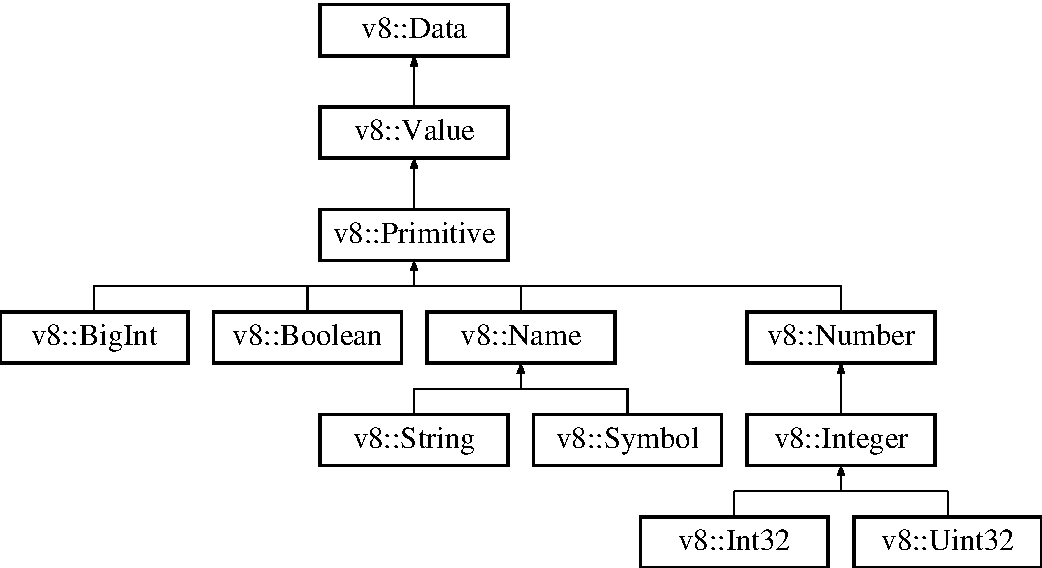
\includegraphics[height=6.000000cm]{classv8_1_1Primitive}
\end{center}
\end{figure}
\subsection*{Additional Inherited Members}


\subsection{Detailed Description}
The superclass of primitive values. See E\+C\+M\+A-\/262 4.\+3.\+2. 

The documentation for this class was generated from the following file\+:\begin{DoxyCompactItemize}
\item 
v8/include/v8.\+h\end{DoxyCompactItemize}

\hypertarget{classv8_1_1Promise}{}\section{v8\+:\+:Promise Class Reference}
\label{classv8_1_1Promise}\index{v8\+::\+Promise@{v8\+::\+Promise}}


{\ttfamily \#include $<$v8.\+h$>$}

Inheritance diagram for v8\+:\+:Promise\+:\begin{figure}[H]
\begin{center}
\leavevmode
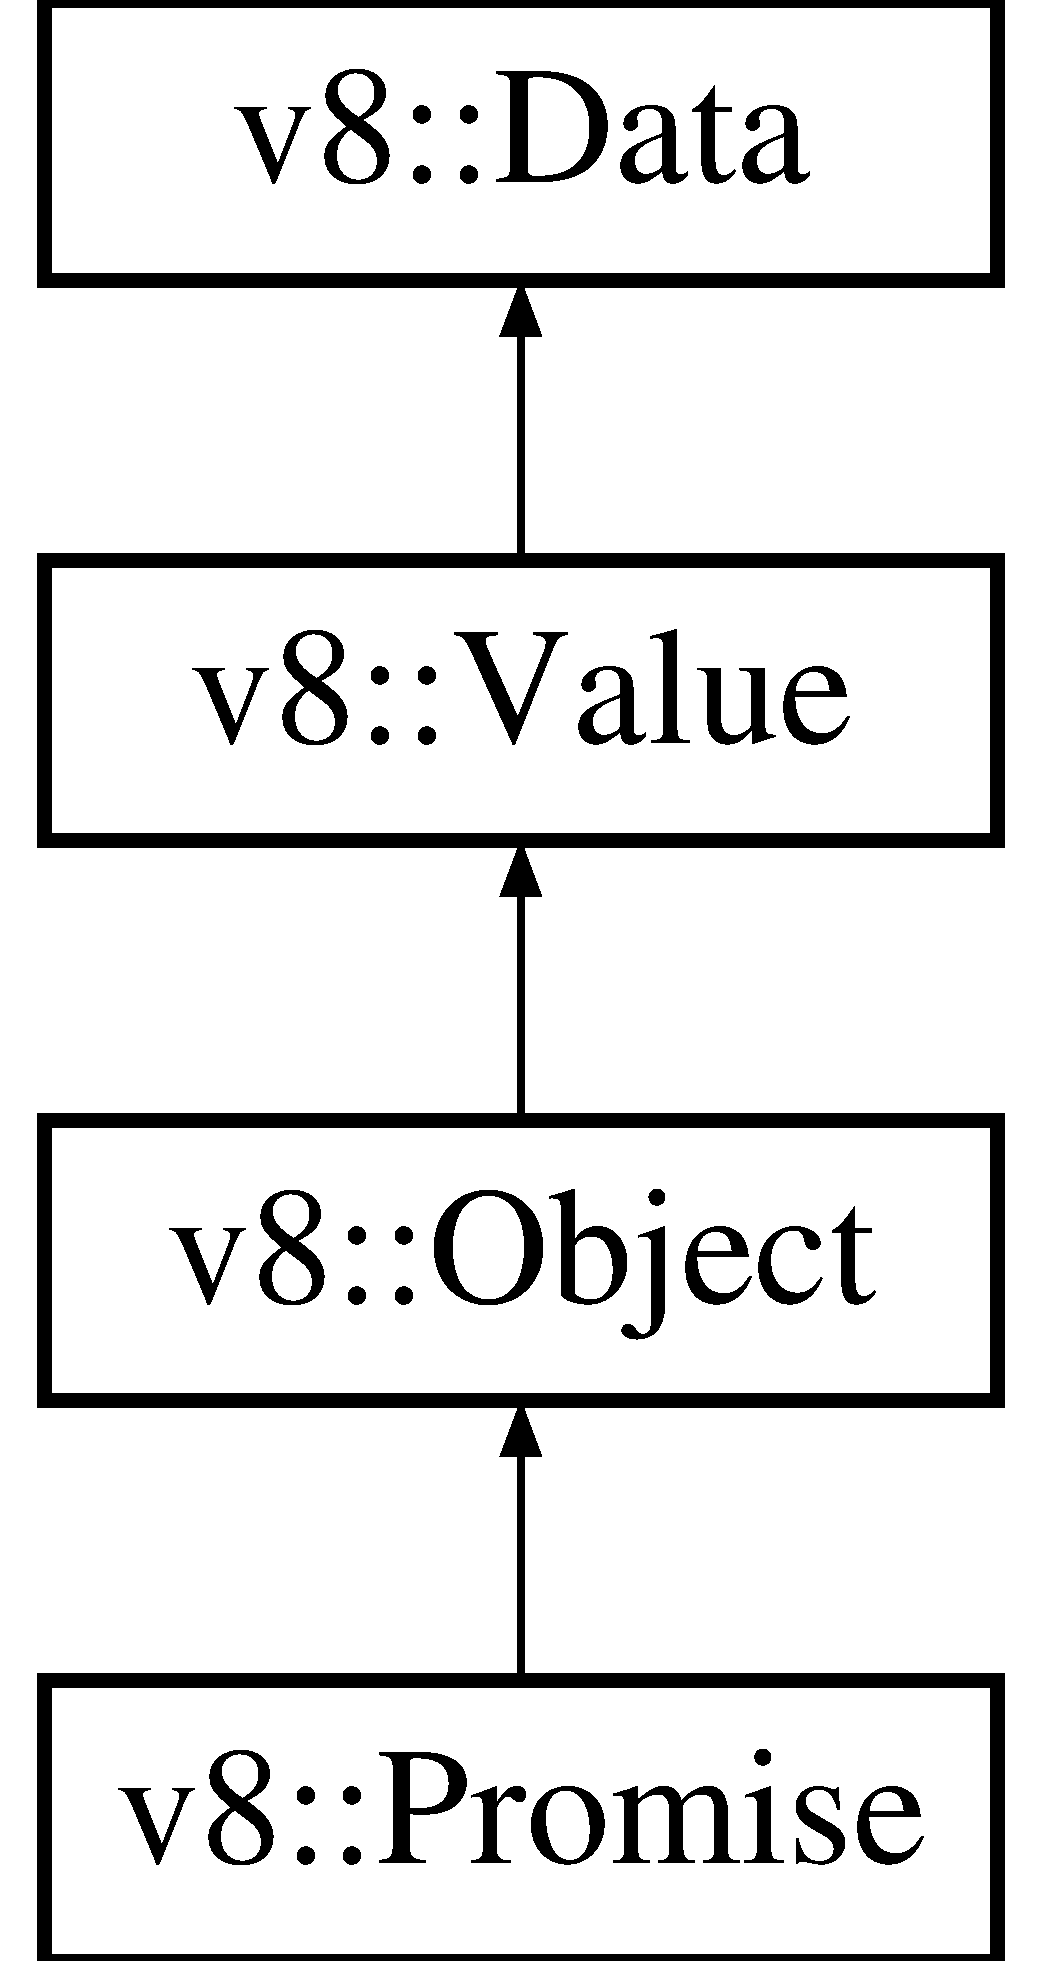
\includegraphics[height=4.000000cm]{classv8_1_1Promise}
\end{center}
\end{figure}
\subsection*{Data Structures}
\begin{DoxyCompactItemize}
\item 
class \hyperlink{classv8_1_1Promise_1_1Resolver}{Resolver}
\end{DoxyCompactItemize}
\subsection*{Public Member Functions}
\begin{DoxyCompactItemize}
\item 
\hyperlink{classv8_1_1Local}{Local}$<$ \hyperlink{classv8_1_1Promise}{Promise} $>$ \hyperlink{classv8_1_1Promise_af56616dc11de23d6d515b0fa5d42e1eb}{Chain} (\hyperlink{classv8_1_1Handle}{Handle}$<$ \hyperlink{classv8_1_1Function}{Function} $>$ handler)
\item 
\hypertarget{classv8_1_1Promise_aab3dea5d0875e1506b9c8fc822b0e005}{}\hyperlink{classv8_1_1Local}{Local}$<$ \hyperlink{classv8_1_1Promise}{Promise} $>$ {\bfseries Catch} (\hyperlink{classv8_1_1Handle}{Handle}$<$ \hyperlink{classv8_1_1Function}{Function} $>$ handler)\label{classv8_1_1Promise_aab3dea5d0875e1506b9c8fc822b0e005}

\item 
\hypertarget{classv8_1_1Promise_a22a7ce609a7ddf0b15bf316e61b0178f}{}\hyperlink{classv8_1_1Local}{Local}$<$ \hyperlink{classv8_1_1Promise}{Promise} $>$ {\bfseries Then} (\hyperlink{classv8_1_1Handle}{Handle}$<$ \hyperlink{classv8_1_1Function}{Function} $>$ handler)\label{classv8_1_1Promise_a22a7ce609a7ddf0b15bf316e61b0178f}

\item 
bool \hyperlink{classv8_1_1Promise_aeea8bdfdbe2291632d7f0d45394c1722}{Has\+Handler} ()
\end{DoxyCompactItemize}
\subsection*{Static Public Member Functions}
\begin{DoxyCompactItemize}
\item 
\hypertarget{classv8_1_1Promise_adfa3b953beb2678dd3b5d6ddb3f0746d}{}static V8\+\_\+\+I\+N\+L\+I\+N\+E \hyperlink{classv8_1_1Promise}{Promise} $\ast$ {\bfseries Cast} (\hyperlink{classv8_1_1Value}{Value} $\ast$obj)\label{classv8_1_1Promise_adfa3b953beb2678dd3b5d6ddb3f0746d}

\end{DoxyCompactItemize}


\subsection{Detailed Description}
An instance of the built-\/in \hyperlink{classv8_1_1Promise}{Promise} constructor (E\+S6 draft). This A\+P\+I is experimental. Only works with --harmony flag. 

\subsection{Member Function Documentation}
\hypertarget{classv8_1_1Promise_af56616dc11de23d6d515b0fa5d42e1eb}{}\index{v8\+::\+Promise@{v8\+::\+Promise}!Chain@{Chain}}
\index{Chain@{Chain}!v8\+::\+Promise@{v8\+::\+Promise}}
\subsubsection[{Chain}]{\setlength{\rightskip}{0pt plus 5cm}{\bf Local}$<${\bf Promise}$>$ v8\+::\+Promise\+::\+Chain (
\begin{DoxyParamCaption}
\item[{{\bf Handle}$<$ {\bf Function} $>$}]{handler}
\end{DoxyParamCaption}
)}\label{classv8_1_1Promise_af56616dc11de23d6d515b0fa5d42e1eb}
Register a resolution/rejection handler with a promise. The handler is given the respective resolution/rejection value as an argument. If the promise is already resolved/rejected, the handler is invoked at the end of turn. \hypertarget{classv8_1_1Promise_aeea8bdfdbe2291632d7f0d45394c1722}{}\index{v8\+::\+Promise@{v8\+::\+Promise}!Has\+Handler@{Has\+Handler}}
\index{Has\+Handler@{Has\+Handler}!v8\+::\+Promise@{v8\+::\+Promise}}
\subsubsection[{Has\+Handler}]{\setlength{\rightskip}{0pt plus 5cm}bool v8\+::\+Promise\+::\+Has\+Handler (
\begin{DoxyParamCaption}
{}
\end{DoxyParamCaption}
)}\label{classv8_1_1Promise_aeea8bdfdbe2291632d7f0d45394c1722}
Returns true if the promise has at least one derived promise, and therefore resolve/reject handlers (including default handler). 

The documentation for this class was generated from the following file\+:\begin{DoxyCompactItemize}
\item 
v8/include/v8.\+h\end{DoxyCompactItemize}

\hypertarget{classv8_1_1PromiseRejectMessage}{}\section{v8\+:\+:Promise\+Reject\+Message Class Reference}
\label{classv8_1_1PromiseRejectMessage}\index{v8\+::\+Promise\+Reject\+Message@{v8\+::\+Promise\+Reject\+Message}}
\subsection*{Public Member Functions}
\begin{DoxyCompactItemize}
\item 
{\bfseries Promise\+Reject\+Message} (\hyperlink{classv8_1_1Local}{Local}$<$ \hyperlink{classv8_1_1Promise}{Promise} $>$ promise, Promise\+Reject\+Event event, \hyperlink{classv8_1_1Local}{Local}$<$ \hyperlink{classv8_1_1Value}{Value} $>$ value, \hyperlink{classv8_1_1Local}{Local}$<$ \hyperlink{classv8_1_1StackTrace}{Stack\+Trace} $>$ stack\+\_\+trace)\hypertarget{classv8_1_1PromiseRejectMessage_a052df173c75f1eb31b252714c88f3362}{}\label{classv8_1_1PromiseRejectMessage_a052df173c75f1eb31b252714c88f3362}

\item 
V8\+\_\+\+I\+N\+L\+I\+NE \hyperlink{classv8_1_1Local}{Local}$<$ \hyperlink{classv8_1_1Promise}{Promise} $>$ {\bfseries Get\+Promise} () const \hypertarget{classv8_1_1PromiseRejectMessage_a8582107385b66f911c6d4c9a17890222}{}\label{classv8_1_1PromiseRejectMessage_a8582107385b66f911c6d4c9a17890222}

\item 
V8\+\_\+\+I\+N\+L\+I\+NE Promise\+Reject\+Event {\bfseries Get\+Event} () const \hypertarget{classv8_1_1PromiseRejectMessage_a1380024500dac27eb74665701a80c6b0}{}\label{classv8_1_1PromiseRejectMessage_a1380024500dac27eb74665701a80c6b0}

\item 
V8\+\_\+\+I\+N\+L\+I\+NE \hyperlink{classv8_1_1Local}{Local}$<$ \hyperlink{classv8_1_1Value}{Value} $>$ {\bfseries Get\+Value} () const \hypertarget{classv8_1_1PromiseRejectMessage_ad87ec78d2e817b623d996f8db7d45ffc}{}\label{classv8_1_1PromiseRejectMessage_ad87ec78d2e817b623d996f8db7d45ffc}

\item 
{\bfseries V8\+\_\+\+D\+E\+P\+R\+E\+C\+A\+T\+ED} (\char`\"{}Use \hyperlink{classv8_1_1Exception_a8d575a721cf0fd5b325afb8b586c0d1e}{v8\+::\+Exception\+::\+Create\+Message}(Get\+Value())-\/$>$Get\+Stack\+Trace()\char`\"{}, V8\+\_\+\+I\+N\+L\+I\+NE \hyperlink{classv8_1_1Local}{Local}$<$ \hyperlink{classv8_1_1StackTrace}{Stack\+Trace} $>$ Get\+Stack\+Trace() const)\hypertarget{classv8_1_1PromiseRejectMessage_af768aa21023875a4037d797d1e91fe42}{}\label{classv8_1_1PromiseRejectMessage_af768aa21023875a4037d797d1e91fe42}

\end{DoxyCompactItemize}


The documentation for this class was generated from the following file\+:\begin{DoxyCompactItemize}
\item 
v8/include/v8.\+h\end{DoxyCompactItemize}

\hypertarget{classv8_1_1PropertyCallbackInfo}{\section{v8\-:\-:Property\-Callback\-Info$<$ T $>$ Class Template Reference}
\label{classv8_1_1PropertyCallbackInfo}\index{v8\-::\-Property\-Callback\-Info$<$ T $>$@{v8\-::\-Property\-Callback\-Info$<$ T $>$}}
}


{\ttfamily \#include $<$v8.\-h$>$}

\subsection*{Public Member Functions}
\begin{DoxyCompactItemize}
\item 
\hypertarget{classv8_1_1PropertyCallbackInfo_a066d0c9eee98f80fb78d97961eafa8ad}{V8\-\_\-\-I\-N\-L\-I\-N\-E \hyperlink{classv8_1_1Isolate}{Isolate} $\ast$ {\bfseries Get\-Isolate} () const }\label{classv8_1_1PropertyCallbackInfo_a066d0c9eee98f80fb78d97961eafa8ad}

\item 
\hypertarget{classv8_1_1PropertyCallbackInfo_a64edbaeb902e360fc2a4d353c8c4930f}{V8\-\_\-\-I\-N\-L\-I\-N\-E \hyperlink{classv8_1_1Local}{Local}$<$ \hyperlink{classv8_1_1Value}{Value} $>$ {\bfseries Data} () const }\label{classv8_1_1PropertyCallbackInfo_a64edbaeb902e360fc2a4d353c8c4930f}

\item 
\hypertarget{classv8_1_1PropertyCallbackInfo_a97c1cf0e962504210ddcb1eacd7af85a}{V8\-\_\-\-I\-N\-L\-I\-N\-E \hyperlink{classv8_1_1Local}{Local}$<$ \hyperlink{classv8_1_1Value}{Value} $>$ {\bfseries This} () const }\label{classv8_1_1PropertyCallbackInfo_a97c1cf0e962504210ddcb1eacd7af85a}

\item 
\hypertarget{classv8_1_1PropertyCallbackInfo_a8eb97205ce7bd25b446b03643d02570d}{V8\-\_\-\-I\-N\-L\-I\-N\-E \hyperlink{classv8_1_1Local}{Local}$<$ \hyperlink{classv8_1_1Object}{Object} $>$ {\bfseries Holder} () const }\label{classv8_1_1PropertyCallbackInfo_a8eb97205ce7bd25b446b03643d02570d}

\item 
\hypertarget{classv8_1_1PropertyCallbackInfo_a4e9bc4da66ed3ea21aac7dbb9c11465b}{V8\-\_\-\-I\-N\-L\-I\-N\-E \hyperlink{classv8_1_1ReturnValue}{Return\-Value}$<$ T $>$ {\bfseries Get\-Return\-Value} () const }\label{classv8_1_1PropertyCallbackInfo_a4e9bc4da66ed3ea21aac7dbb9c11465b}

\end{DoxyCompactItemize}
\subsection*{Static Public Attributes}
\begin{DoxyCompactItemize}
\item 
\hypertarget{classv8_1_1PropertyCallbackInfo_a9fc9663a2e23f9324fe61f92d1e7e5b5}{static const int {\bfseries k\-Args\-Length} = 6}\label{classv8_1_1PropertyCallbackInfo_a9fc9663a2e23f9324fe61f92d1e7e5b5}

\end{DoxyCompactItemize}
\subsection*{Protected Member Functions}
\begin{DoxyCompactItemize}
\item 
\hypertarget{classv8_1_1PropertyCallbackInfo_aa666043c86d4db9a57a3ac866c78ee0e}{V8\-\_\-\-I\-N\-L\-I\-N\-E {\bfseries Property\-Callback\-Info} (internal\-::\-Object $\ast$$\ast$args)}\label{classv8_1_1PropertyCallbackInfo_aa666043c86d4db9a57a3ac866c78ee0e}

\end{DoxyCompactItemize}
\subsection*{Protected Attributes}
\begin{DoxyCompactItemize}
\item 
\hypertarget{classv8_1_1PropertyCallbackInfo_a57b2243627071c62ed3900a741a41a0b}{internal\-::\-Object $\ast$$\ast$ {\bfseries args\-\_\-}}\label{classv8_1_1PropertyCallbackInfo_a57b2243627071c62ed3900a741a41a0b}

\end{DoxyCompactItemize}
\subsection*{Static Protected Attributes}
\begin{DoxyCompactItemize}
\item 
\hypertarget{classv8_1_1PropertyCallbackInfo_a8598985473483dfadba4e4c67251675b}{static const int {\bfseries k\-Holder\-Index} = 0}\label{classv8_1_1PropertyCallbackInfo_a8598985473483dfadba4e4c67251675b}

\item 
\hypertarget{classv8_1_1PropertyCallbackInfo_a59ba899cb580bc5e8adca6f799db3e2a}{static const int {\bfseries k\-Isolate\-Index} = 1}\label{classv8_1_1PropertyCallbackInfo_a59ba899cb580bc5e8adca6f799db3e2a}

\item 
\hypertarget{classv8_1_1PropertyCallbackInfo_a00849f770023891d1466176f5e0c8539}{static const int {\bfseries k\-Return\-Value\-Default\-Value\-Index} = 2}\label{classv8_1_1PropertyCallbackInfo_a00849f770023891d1466176f5e0c8539}

\item 
\hypertarget{classv8_1_1PropertyCallbackInfo_ae16cdf2c6ce787b21d94953cd514ed0e}{static const int {\bfseries k\-Return\-Value\-Index} = 3}\label{classv8_1_1PropertyCallbackInfo_ae16cdf2c6ce787b21d94953cd514ed0e}

\item 
\hypertarget{classv8_1_1PropertyCallbackInfo_a39fc5d6aaccb2916af503c7120ab99c5}{static const int {\bfseries k\-Data\-Index} = 4}\label{classv8_1_1PropertyCallbackInfo_a39fc5d6aaccb2916af503c7120ab99c5}

\item 
\hypertarget{classv8_1_1PropertyCallbackInfo_a715d28b9c57a581de1698673c9b9eb8a}{static const int {\bfseries k\-This\-Index} = 5}\label{classv8_1_1PropertyCallbackInfo_a715d28b9c57a581de1698673c9b9eb8a}

\end{DoxyCompactItemize}
\subsection*{Friends}
\begin{DoxyCompactItemize}
\item 
\hypertarget{classv8_1_1PropertyCallbackInfo_ae605ff1d9d93250ace8a0a8b8d1dee67}{class {\bfseries Macro\-Assembler}}\label{classv8_1_1PropertyCallbackInfo_ae605ff1d9d93250ace8a0a8b8d1dee67}

\item 
\hypertarget{classv8_1_1PropertyCallbackInfo_a1ba96a1268a72c23f50314cd99c76f1b}{class {\bfseries internal\-::\-Property\-Callback\-Arguments}}\label{classv8_1_1PropertyCallbackInfo_a1ba96a1268a72c23f50314cd99c76f1b}

\item 
\hypertarget{classv8_1_1PropertyCallbackInfo_ad1d1e15ddaed2ab44e8f21c5564881ba}{class {\bfseries internal\-::\-Custom\-Arguments$<$ Property\-Callback\-Info $>$}}\label{classv8_1_1PropertyCallbackInfo_ad1d1e15ddaed2ab44e8f21c5564881ba}

\end{DoxyCompactItemize}


\subsection{Detailed Description}
\subsubsection*{template$<$typename T$>$class v8\-::\-Property\-Callback\-Info$<$ T $>$}

The information passed to a property callback about the context of the property access. 

The documentation for this class was generated from the following file\-:\begin{DoxyCompactItemize}
\item 
v8/include/v8.\-h\end{DoxyCompactItemize}

\hypertarget{classv8_1_1RegExp}{}\section{v8\+:\+:Reg\+Exp Class Reference}
\label{classv8_1_1RegExp}\index{v8\+::\+Reg\+Exp@{v8\+::\+Reg\+Exp}}


{\ttfamily \#include $<$v8.\+h$>$}

Inheritance diagram for v8\+:\+:Reg\+Exp\+:\begin{figure}[H]
\begin{center}
\leavevmode
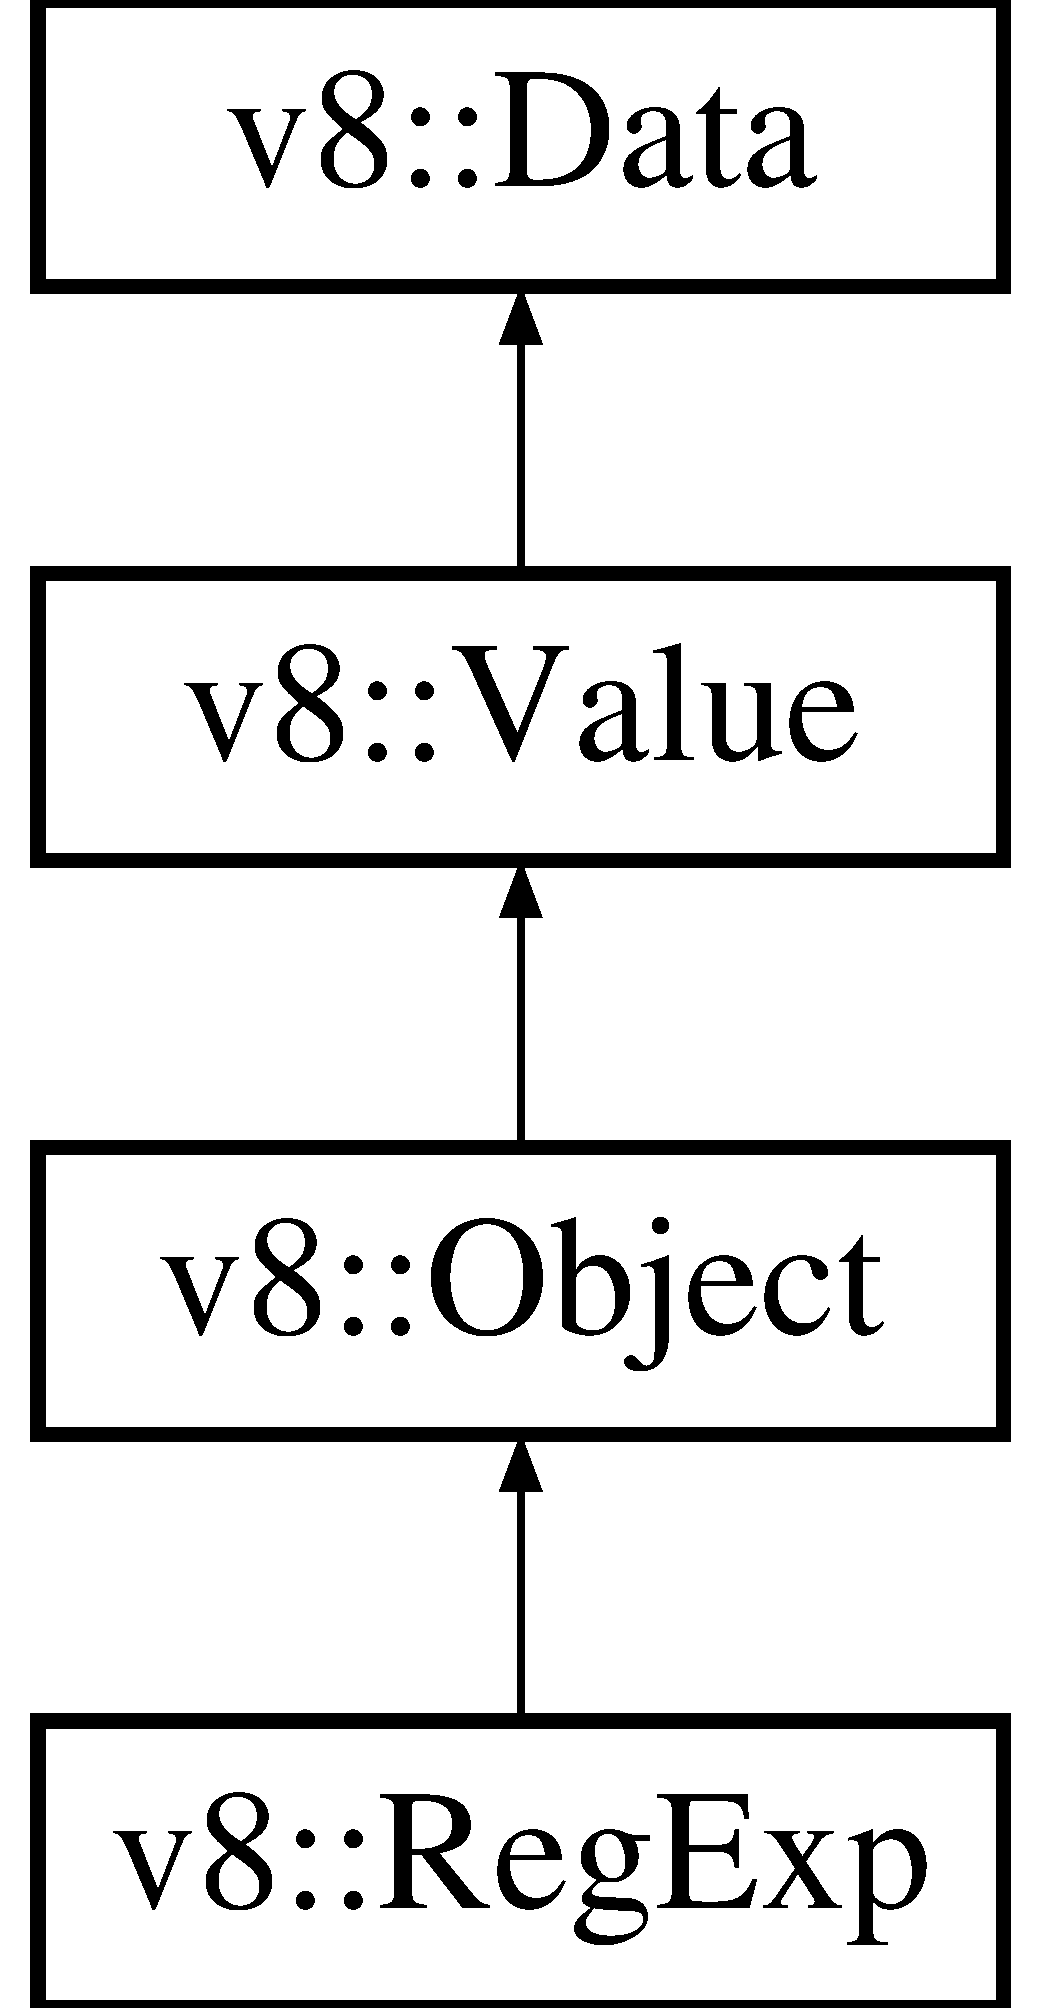
\includegraphics[height=4.000000cm]{classv8_1_1RegExp}
\end{center}
\end{figure}
\subsection*{Public Types}
\begin{DoxyCompactItemize}
\item 
enum \hyperlink{classv8_1_1RegExp_aa4718a5c1f18472aff3bf51ed694fc5a}{Flags} \{ {\bfseries k\+None} = 0, 
{\bfseries k\+Global} = 1, 
{\bfseries k\+Ignore\+Case} = 2, 
{\bfseries k\+Multiline} = 4
 \}
\end{DoxyCompactItemize}
\subsection*{Public Member Functions}
\begin{DoxyCompactItemize}
\item 
\hyperlink{classv8_1_1Local}{Local}$<$ \hyperlink{classv8_1_1String}{String} $>$ \hyperlink{classv8_1_1RegExp_a448213f2a92d964ed260b51429d5e590}{Get\+Source} () const 
\item 
\hyperlink{classv8_1_1RegExp_aa4718a5c1f18472aff3bf51ed694fc5a}{Flags} \hyperlink{classv8_1_1RegExp_ad5a5e77e6e626b3c7c69eef7ba2908cc}{Get\+Flags} () const 
\end{DoxyCompactItemize}
\subsection*{Static Public Member Functions}
\begin{DoxyCompactItemize}
\item 
static \hyperlink{classv8_1_1Local}{Local}$<$ \hyperlink{classv8_1_1RegExp}{Reg\+Exp} $>$ \hyperlink{classv8_1_1RegExp_ac92fcff5a40cf8c698aefd021c823c2e}{New} (\hyperlink{classv8_1_1Handle}{Handle}$<$ \hyperlink{classv8_1_1String}{String} $>$ pattern, \hyperlink{classv8_1_1RegExp_aa4718a5c1f18472aff3bf51ed694fc5a}{Flags} flags)
\item 
\hypertarget{classv8_1_1RegExp_ac06d8f61c0ebb2e7292e6aeff7108f26}{}static V8\+\_\+\+I\+N\+L\+I\+N\+E \hyperlink{classv8_1_1RegExp}{Reg\+Exp} $\ast$ {\bfseries Cast} (\hyperlink{classv8_1_1Value}{v8\+::\+Value} $\ast$obj)\label{classv8_1_1RegExp_ac06d8f61c0ebb2e7292e6aeff7108f26}

\end{DoxyCompactItemize}


\subsection{Detailed Description}
An instance of the built-\/in \hyperlink{classv8_1_1RegExp}{Reg\+Exp} constructor (E\+C\+M\+A-\/262, 15.\+10). 

\subsection{Member Enumeration Documentation}
\hypertarget{classv8_1_1RegExp_aa4718a5c1f18472aff3bf51ed694fc5a}{}\index{v8\+::\+Reg\+Exp@{v8\+::\+Reg\+Exp}!Flags@{Flags}}
\index{Flags@{Flags}!v8\+::\+Reg\+Exp@{v8\+::\+Reg\+Exp}}
\subsubsection[{Flags}]{\setlength{\rightskip}{0pt plus 5cm}enum {\bf v8\+::\+Reg\+Exp\+::\+Flags}}\label{classv8_1_1RegExp_aa4718a5c1f18472aff3bf51ed694fc5a}
Regular expression flag bits. They can be or\textquotesingle{}ed to enable a set of flags. 

\subsection{Member Function Documentation}
\hypertarget{classv8_1_1RegExp_ad5a5e77e6e626b3c7c69eef7ba2908cc}{}\index{v8\+::\+Reg\+Exp@{v8\+::\+Reg\+Exp}!Get\+Flags@{Get\+Flags}}
\index{Get\+Flags@{Get\+Flags}!v8\+::\+Reg\+Exp@{v8\+::\+Reg\+Exp}}
\subsubsection[{Get\+Flags}]{\setlength{\rightskip}{0pt plus 5cm}{\bf Flags} v8\+::\+Reg\+Exp\+::\+Get\+Flags (
\begin{DoxyParamCaption}
{}
\end{DoxyParamCaption}
) const}\label{classv8_1_1RegExp_ad5a5e77e6e626b3c7c69eef7ba2908cc}
Returns the flags bit field. \hypertarget{classv8_1_1RegExp_a448213f2a92d964ed260b51429d5e590}{}\index{v8\+::\+Reg\+Exp@{v8\+::\+Reg\+Exp}!Get\+Source@{Get\+Source}}
\index{Get\+Source@{Get\+Source}!v8\+::\+Reg\+Exp@{v8\+::\+Reg\+Exp}}
\subsubsection[{Get\+Source}]{\setlength{\rightskip}{0pt plus 5cm}{\bf Local}$<${\bf String}$>$ v8\+::\+Reg\+Exp\+::\+Get\+Source (
\begin{DoxyParamCaption}
{}
\end{DoxyParamCaption}
) const}\label{classv8_1_1RegExp_a448213f2a92d964ed260b51429d5e590}
Returns the value of the source property\+: a string representing the regular expression. \hypertarget{classv8_1_1RegExp_ac92fcff5a40cf8c698aefd021c823c2e}{}\index{v8\+::\+Reg\+Exp@{v8\+::\+Reg\+Exp}!New@{New}}
\index{New@{New}!v8\+::\+Reg\+Exp@{v8\+::\+Reg\+Exp}}
\subsubsection[{New}]{\setlength{\rightskip}{0pt plus 5cm}static {\bf Local}$<${\bf Reg\+Exp}$>$ v8\+::\+Reg\+Exp\+::\+New (
\begin{DoxyParamCaption}
\item[{{\bf Handle}$<$ {\bf String} $>$}]{pattern, }
\item[{{\bf Flags}}]{flags}
\end{DoxyParamCaption}
)\hspace{0.3cm}{\ttfamily [static]}}\label{classv8_1_1RegExp_ac92fcff5a40cf8c698aefd021c823c2e}
Creates a regular expression from the given pattern string and the flags bit field. May throw a Java\+Script exception as described in E\+C\+M\+A-\/262, 15.\+10.\+4.\+1.

For example, \hyperlink{classv8_1_1RegExp_ac92fcff5a40cf8c698aefd021c823c2e}{Reg\+Exp\+::\+New}(v8\+::\+String\+::\+New(\char`\"{}foo\char`\"{}), static\+\_\+cast$<$\+Reg\+Exp\+::\+Flags$>$(k\+Global $\vert$ k\+Multiline)) is equivalent to evaluating \char`\"{}/foo/gm\char`\"{}. 

The documentation for this class was generated from the following file\+:\begin{DoxyCompactItemize}
\item 
v8/include/v8.\+h\end{DoxyCompactItemize}

\hypertarget{structv8_1_1RegisterState}{}\section{v8\+:\+:Register\+State Struct Reference}
\label{structv8_1_1RegisterState}\index{v8\+::\+Register\+State@{v8\+::\+Register\+State}}
\subsection*{Data Fields}
\begin{DoxyCompactItemize}
\item 
\mbox{\Hypertarget{structv8_1_1RegisterState_aa0d0327871d9f95d5e64f47b7f183907}\label{structv8_1_1RegisterState_aa0d0327871d9f95d5e64f47b7f183907}} 
void $\ast$ {\bfseries pc}
\item 
\mbox{\Hypertarget{structv8_1_1RegisterState_a867bb9d0b9e81c3f7256aa81dc0daee4}\label{structv8_1_1RegisterState_a867bb9d0b9e81c3f7256aa81dc0daee4}} 
void $\ast$ {\bfseries sp}
\item 
\mbox{\Hypertarget{structv8_1_1RegisterState_aaeb80a1d7f6df3ae418f3e9b1295d156}\label{structv8_1_1RegisterState_aaeb80a1d7f6df3ae418f3e9b1295d156}} 
void $\ast$ {\bfseries fp}
\end{DoxyCompactItemize}


\subsection{Detailed Description}


Definition at line 1809 of file v8.\+h.



The documentation for this struct was generated from the following file\+:\begin{DoxyCompactItemize}
\item 
v8/include/v8.\+h\end{DoxyCompactItemize}

\hypertarget{classv8_1_1Promise_1_1Resolver}{\section{v8\-:\-:Promise\-:\-:Resolver Class Reference}
\label{classv8_1_1Promise_1_1Resolver}\index{v8\-::\-Promise\-::\-Resolver@{v8\-::\-Promise\-::\-Resolver}}
}
Inheritance diagram for v8\-:\-:Promise\-:\-:Resolver\-:\begin{figure}[H]
\begin{center}
\leavevmode
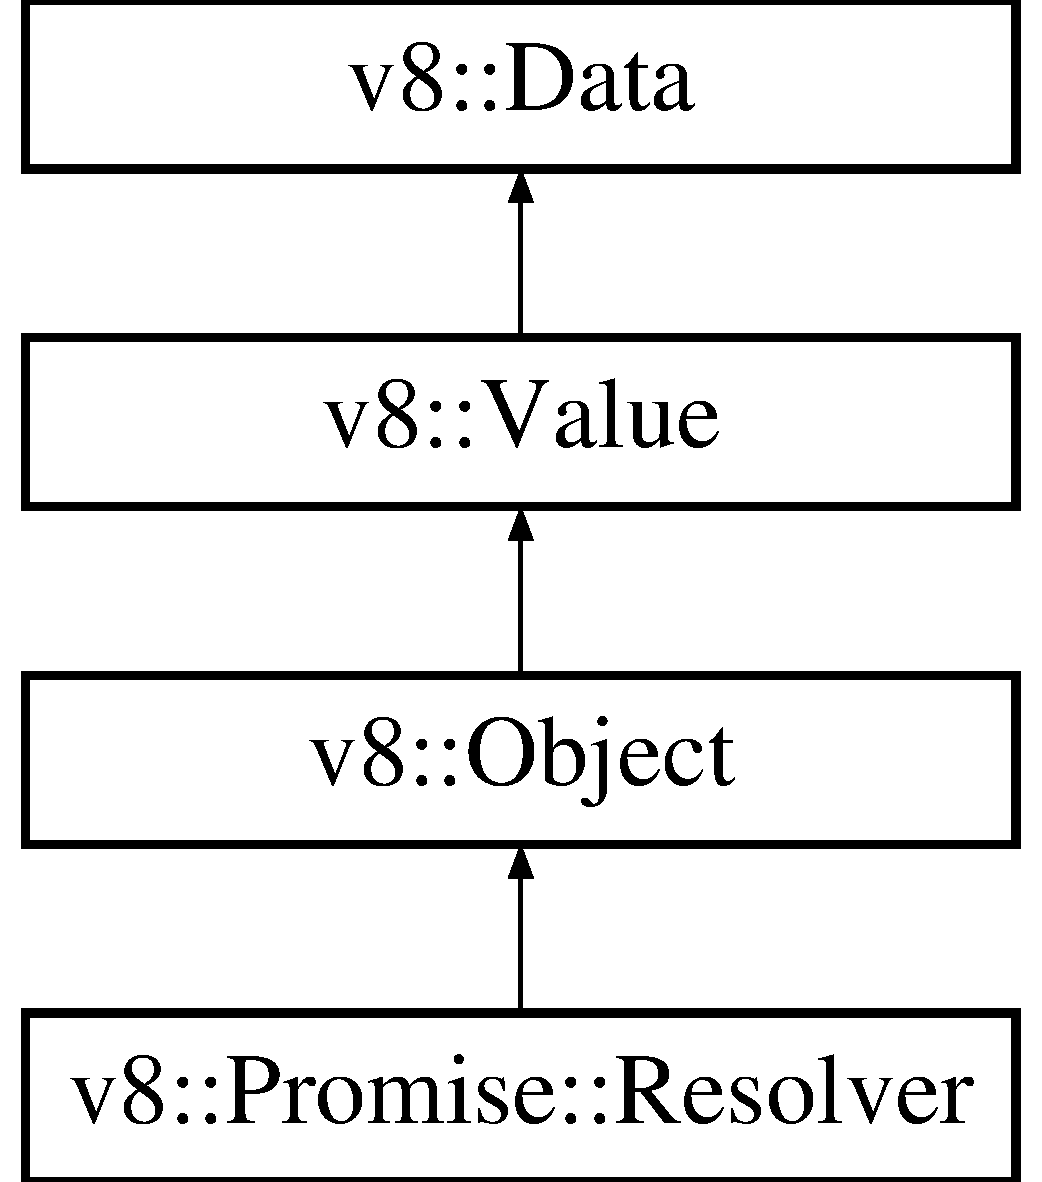
\includegraphics[height=4.000000cm]{classv8_1_1Promise_1_1Resolver}
\end{center}
\end{figure}
\subsection*{Public Member Functions}
\begin{DoxyCompactItemize}
\item 
\hyperlink{classv8_1_1Local}{Local}$<$ \hyperlink{classv8_1_1Promise}{Promise} $>$ \hyperlink{classv8_1_1Promise_1_1Resolver_a41fd1ffef546a62e363a639935fc8ae3}{Get\-Promise} ()
\item 
void \hyperlink{classv8_1_1Promise_1_1Resolver_aa1f7f6883d57879a7956e84e63b2d935}{Resolve} (\hyperlink{classv8_1_1Handle}{Handle}$<$ \hyperlink{classv8_1_1Value}{Value} $>$ value)
\item 
\hypertarget{classv8_1_1Promise_1_1Resolver_a12b1f6ef41dd7d759443631135502847}{void {\bfseries Reject} (\hyperlink{classv8_1_1Handle}{Handle}$<$ \hyperlink{classv8_1_1Value}{Value} $>$ value)}\label{classv8_1_1Promise_1_1Resolver_a12b1f6ef41dd7d759443631135502847}

\end{DoxyCompactItemize}
\subsection*{Static Public Member Functions}
\begin{DoxyCompactItemize}
\item 
static \hyperlink{classv8_1_1Local}{Local}$<$ \hyperlink{classv8_1_1Promise_1_1Resolver}{Resolver} $>$ \hyperlink{classv8_1_1Promise_1_1Resolver_a80b9e402b6b49f41d57d404ed9e00c9d}{New} (\hyperlink{classv8_1_1Isolate}{Isolate} $\ast$isolate)
\item 
\hypertarget{classv8_1_1Promise_1_1Resolver_ab2b541cb210158ed0c757c8b7dc46279}{static V8\-\_\-\-I\-N\-L\-I\-N\-E \hyperlink{classv8_1_1Promise_1_1Resolver}{Resolver} $\ast$ {\bfseries Cast} (\hyperlink{classv8_1_1Value}{Value} $\ast$obj)}\label{classv8_1_1Promise_1_1Resolver_ab2b541cb210158ed0c757c8b7dc46279}

\end{DoxyCompactItemize}


\subsection{Member Function Documentation}
\hypertarget{classv8_1_1Promise_1_1Resolver_a41fd1ffef546a62e363a639935fc8ae3}{\index{v8\-::\-Promise\-::\-Resolver@{v8\-::\-Promise\-::\-Resolver}!Get\-Promise@{Get\-Promise}}
\index{Get\-Promise@{Get\-Promise}!v8::Promise::Resolver@{v8\-::\-Promise\-::\-Resolver}}
\subsubsection[{Get\-Promise}]{\setlength{\rightskip}{0pt plus 5cm}{\bf Local}$<${\bf Promise}$>$ v8\-::\-Promise\-::\-Resolver\-::\-Get\-Promise (
\begin{DoxyParamCaption}
{}
\end{DoxyParamCaption}
)}}\label{classv8_1_1Promise_1_1Resolver_a41fd1ffef546a62e363a639935fc8ae3}
Extract the associated promise. \hypertarget{classv8_1_1Promise_1_1Resolver_a80b9e402b6b49f41d57d404ed9e00c9d}{\index{v8\-::\-Promise\-::\-Resolver@{v8\-::\-Promise\-::\-Resolver}!New@{New}}
\index{New@{New}!v8::Promise::Resolver@{v8\-::\-Promise\-::\-Resolver}}
\subsubsection[{New}]{\setlength{\rightskip}{0pt plus 5cm}static {\bf Local}$<${\bf Resolver}$>$ v8\-::\-Promise\-::\-Resolver\-::\-New (
\begin{DoxyParamCaption}
\item[{{\bf Isolate} $\ast$}]{isolate}
\end{DoxyParamCaption}
)\hspace{0.3cm}{\ttfamily [static]}}}\label{classv8_1_1Promise_1_1Resolver_a80b9e402b6b49f41d57d404ed9e00c9d}
Create a new resolver, along with an associated promise in pending state. 

Reimplemented from \hyperlink{classv8_1_1Object}{v8\-::\-Object}.

\hypertarget{classv8_1_1Promise_1_1Resolver_aa1f7f6883d57879a7956e84e63b2d935}{\index{v8\-::\-Promise\-::\-Resolver@{v8\-::\-Promise\-::\-Resolver}!Resolve@{Resolve}}
\index{Resolve@{Resolve}!v8::Promise::Resolver@{v8\-::\-Promise\-::\-Resolver}}
\subsubsection[{Resolve}]{\setlength{\rightskip}{0pt plus 5cm}void v8\-::\-Promise\-::\-Resolver\-::\-Resolve (
\begin{DoxyParamCaption}
\item[{{\bf Handle}$<$ {\bf Value} $>$}]{value}
\end{DoxyParamCaption}
)}}\label{classv8_1_1Promise_1_1Resolver_aa1f7f6883d57879a7956e84e63b2d935}
Resolve/reject the associated promise with a given value. Ignored if the promise is no longer pending. 

The documentation for this class was generated from the following file\-:\begin{DoxyCompactItemize}
\item 
v8/include/v8.\-h\end{DoxyCompactItemize}

\hypertarget{classv8_1_1ResourceConstraints}{}\section{v8\+:\+:Resource\+Constraints Class Reference}
\label{classv8_1_1ResourceConstraints}\index{v8\+::\+Resource\+Constraints@{v8\+::\+Resource\+Constraints}}


{\ttfamily \#include $<$v8.\+h$>$}

\subsection*{Public Member Functions}
\begin{DoxyCompactItemize}
\item 
void \mbox{\hyperlink{classv8_1_1ResourceConstraints_aeeaaee4017e8d5f8f0439af2af2ed3a5}{Configure\+Defaults}} (uint64\+\_\+t physical\+\_\+memory, uint64\+\_\+t virtual\+\_\+memory\+\_\+limit)
\item 
\mbox{\Hypertarget{classv8_1_1ResourceConstraints_ac4d579082c042f7083882599b5fb6d73}\label{classv8_1_1ResourceConstraints_ac4d579082c042f7083882599b5fb6d73}} 
{\bfseries V8\+\_\+\+D\+E\+P\+R\+E\+C\+A\+T\+E\+\_\+\+S\+O\+ON} (\char`\"{}Use max\+\_\+semi\+\_\+space\+\_\+size\+\_\+in\+\_\+kb()\char`\"{}, size\+\_\+t max\+\_\+semi\+\_\+space\+\_\+size())
\item 
\mbox{\Hypertarget{classv8_1_1ResourceConstraints_a9a6ea46da51be9c77d55e2165bdbbd69}\label{classv8_1_1ResourceConstraints_a9a6ea46da51be9c77d55e2165bdbbd69}} 
{\bfseries V8\+\_\+\+D\+E\+P\+R\+E\+C\+A\+T\+E\+\_\+\+S\+O\+ON} (\char`\"{}Use set\+\_\+max\+\_\+semi\+\_\+space\+\_\+size\+\_\+in\+\_\+kb(size\+\_\+t limit\+\_\+in\+\_\+kb)\char`\"{}, void set\+\_\+max\+\_\+semi\+\_\+space\+\_\+size(size\+\_\+t limit\+\_\+in\+\_\+mb))
\item 
\mbox{\Hypertarget{classv8_1_1ResourceConstraints_addfd17b3241d910daf36dc50b6a7799b}\label{classv8_1_1ResourceConstraints_addfd17b3241d910daf36dc50b6a7799b}} 
size\+\_\+t {\bfseries max\+\_\+semi\+\_\+space\+\_\+size\+\_\+in\+\_\+kb} () const
\item 
\mbox{\Hypertarget{classv8_1_1ResourceConstraints_a6ab6168308a1974eb5a09a3a78171e6f}\label{classv8_1_1ResourceConstraints_a6ab6168308a1974eb5a09a3a78171e6f}} 
void {\bfseries set\+\_\+max\+\_\+semi\+\_\+space\+\_\+size\+\_\+in\+\_\+kb} (size\+\_\+t limit\+\_\+in\+\_\+kb)
\item 
\mbox{\Hypertarget{classv8_1_1ResourceConstraints_ab36b6b94c22c7f1e449dd2c337442177}\label{classv8_1_1ResourceConstraints_ab36b6b94c22c7f1e449dd2c337442177}} 
size\+\_\+t {\bfseries max\+\_\+old\+\_\+space\+\_\+size} () const
\item 
\mbox{\Hypertarget{classv8_1_1ResourceConstraints_a3b65a4726a6374b6e206c5ead95dfca4}\label{classv8_1_1ResourceConstraints_a3b65a4726a6374b6e206c5ead95dfca4}} 
void {\bfseries set\+\_\+max\+\_\+old\+\_\+space\+\_\+size} (size\+\_\+t limit\+\_\+in\+\_\+mb)
\item 
\mbox{\Hypertarget{classv8_1_1ResourceConstraints_ac6d9d402595cb4ed096fcf8ace32e27b}\label{classv8_1_1ResourceConstraints_ac6d9d402595cb4ed096fcf8ace32e27b}} 
{\bfseries V8\+\_\+\+D\+E\+P\+R\+E\+C\+A\+T\+E\+\_\+\+S\+O\+ON} (\char`\"{}max\+\_\+executable\+\_\+size\+\_\+ is subsumed by max\+\_\+old\+\_\+space\+\_\+size\+\_\+\char`\"{}, size\+\_\+t max\+\_\+executable\+\_\+size() const)
\item 
\mbox{\Hypertarget{classv8_1_1ResourceConstraints_ab05d877a81d3dfa5b52e631a66829413}\label{classv8_1_1ResourceConstraints_ab05d877a81d3dfa5b52e631a66829413}} 
{\bfseries V8\+\_\+\+D\+E\+P\+R\+E\+C\+A\+T\+E\+\_\+\+S\+O\+ON} (\char`\"{}max\+\_\+executable\+\_\+size\+\_\+ is subsumed by max\+\_\+old\+\_\+space\+\_\+size\+\_\+\char`\"{}, void set\+\_\+max\+\_\+executable\+\_\+size(size\+\_\+t limit\+\_\+in\+\_\+mb))
\item 
\mbox{\Hypertarget{classv8_1_1ResourceConstraints_ac65767ca8638b69206a7a8f3651641f2}\label{classv8_1_1ResourceConstraints_ac65767ca8638b69206a7a8f3651641f2}} 
uint32\+\_\+t $\ast$ {\bfseries stack\+\_\+limit} () const
\item 
\mbox{\Hypertarget{classv8_1_1ResourceConstraints_a26ed3e89985a4afe34e84509fb093cf1}\label{classv8_1_1ResourceConstraints_a26ed3e89985a4afe34e84509fb093cf1}} 
void {\bfseries set\+\_\+stack\+\_\+limit} (uint32\+\_\+t $\ast$value)
\item 
\mbox{\Hypertarget{classv8_1_1ResourceConstraints_ad97a22955d12a30c9e1634c58a06bb00}\label{classv8_1_1ResourceConstraints_ad97a22955d12a30c9e1634c58a06bb00}} 
size\+\_\+t {\bfseries code\+\_\+range\+\_\+size} () const
\item 
\mbox{\Hypertarget{classv8_1_1ResourceConstraints_adeab824b969292881098b66164ab9e13}\label{classv8_1_1ResourceConstraints_adeab824b969292881098b66164ab9e13}} 
void {\bfseries set\+\_\+code\+\_\+range\+\_\+size} (size\+\_\+t limit\+\_\+in\+\_\+mb)
\item 
\mbox{\Hypertarget{classv8_1_1ResourceConstraints_ae8506ba44debf9d857bc10e72c4031a4}\label{classv8_1_1ResourceConstraints_ae8506ba44debf9d857bc10e72c4031a4}} 
size\+\_\+t {\bfseries max\+\_\+zone\+\_\+pool\+\_\+size} () const
\item 
\mbox{\Hypertarget{classv8_1_1ResourceConstraints_a1d32bdb9913fe3b35fba04ddc408d922}\label{classv8_1_1ResourceConstraints_a1d32bdb9913fe3b35fba04ddc408d922}} 
void {\bfseries set\+\_\+max\+\_\+zone\+\_\+pool\+\_\+size} (size\+\_\+t bytes)
\end{DoxyCompactItemize}


\subsection{Detailed Description}
A set of constraints that specifies the limits of the runtime\textquotesingle{}s memory use. You must set the heap size before initializing the VM -\/ the size cannot be adjusted after the VM is initialized.

If you are using threads then you should hold the V8\+::\+Locker lock while setting the stack limit and you must set a non-\/default stack limit separately for each thread.

The arguments for set\+\_\+max\+\_\+semi\+\_\+space\+\_\+size, set\+\_\+max\+\_\+old\+\_\+space\+\_\+size, set\+\_\+max\+\_\+executable\+\_\+size, set\+\_\+code\+\_\+range\+\_\+size specify limits in MB.

The argument for set\+\_\+max\+\_\+semi\+\_\+space\+\_\+size\+\_\+in\+\_\+kb is in KB. 

\subsection{Member Function Documentation}
\mbox{\Hypertarget{classv8_1_1ResourceConstraints_aeeaaee4017e8d5f8f0439af2af2ed3a5}\label{classv8_1_1ResourceConstraints_aeeaaee4017e8d5f8f0439af2af2ed3a5}} 
\index{v8\+::\+Resource\+Constraints@{v8\+::\+Resource\+Constraints}!Configure\+Defaults@{Configure\+Defaults}}
\index{Configure\+Defaults@{Configure\+Defaults}!v8\+::\+Resource\+Constraints@{v8\+::\+Resource\+Constraints}}
\subsubsection{\texorpdfstring{Configure\+Defaults()}{ConfigureDefaults()}}
{\footnotesize\ttfamily void v8\+::\+Resource\+Constraints\+::\+Configure\+Defaults (\begin{DoxyParamCaption}\item[{uint64\+\_\+t}]{physical\+\_\+memory,  }\item[{uint64\+\_\+t}]{virtual\+\_\+memory\+\_\+limit }\end{DoxyParamCaption})}

Configures the constraints with reasonable default values based on the capabilities of the current device the VM is running on.


\begin{DoxyParams}{Parameters}
{\em physical\+\_\+memory} & The total amount of physical memory on the current device, in bytes. \\
\hline
{\em virtual\+\_\+memory\+\_\+limit} & The amount of virtual memory on the current device, in bytes, or zero, if there is no limit. \\
\hline
\end{DoxyParams}


The documentation for this class was generated from the following file\+:\begin{DoxyCompactItemize}
\item 
v8/include/v8.\+h\end{DoxyCompactItemize}

\hypertarget{classv8_1_1RetainedObjectInfo}{}\section{v8\+:\+:Retained\+Object\+Info Class Reference}
\label{classv8_1_1RetainedObjectInfo}\index{v8\+::\+Retained\+Object\+Info@{v8\+::\+Retained\+Object\+Info}}


{\ttfamily \#include $<$v8-\/profiler.\+h$>$}

\subsection*{Public Member Functions}
\begin{DoxyCompactItemize}
\item 
virtual void \mbox{\hyperlink{classv8_1_1RetainedObjectInfo_a5011203f7c5949049ba36b8059f03eca}{Dispose}} ()=0
\item 
virtual bool \mbox{\hyperlink{classv8_1_1RetainedObjectInfo_a286103bb076c85415919c86b1838c990}{Is\+Equivalent}} (\mbox{\hyperlink{classv8_1_1RetainedObjectInfo}{Retained\+Object\+Info}} $\ast$other)=0
\item 
virtual intptr\+\_\+t \mbox{\hyperlink{classv8_1_1RetainedObjectInfo_a6fdbfa242b95615e63f08433419c8066}{Get\+Hash}} ()=0
\item 
virtual const char $\ast$ \mbox{\hyperlink{classv8_1_1RetainedObjectInfo_ad19106fc7f0499fd45005077551d54c0}{Get\+Label}} ()=0
\item 
virtual const char $\ast$ \mbox{\hyperlink{classv8_1_1RetainedObjectInfo_adf835370c5516f2a89dd2d3f83dee10b}{Get\+Group\+Label}} ()
\item 
virtual intptr\+\_\+t \mbox{\hyperlink{classv8_1_1RetainedObjectInfo_ae6865597469bc7d28bd8ec71b4b890bd}{Get\+Element\+Count}} ()
\item 
virtual intptr\+\_\+t \mbox{\hyperlink{classv8_1_1RetainedObjectInfo_a1a899eed0b1f6e046edc3c7a7c08aa8c}{Get\+Size\+In\+Bytes}} ()
\end{DoxyCompactItemize}


\subsection{Detailed Description}
Interface for providing information about embedder\textquotesingle{}s objects held by global handles. This information is reported in two ways\+:


\begin{DoxyEnumerate}
\item When calling Add\+Object\+Group, an embedder may pass \mbox{\hyperlink{classv8_1_1RetainedObjectInfo}{Retained\+Object\+Info}} instance describing the group. To collect this information while taking a heap snapshot, \mbox{\hyperlink{classv8_1_1V8}{V8}} calls GC prologue and epilogue callbacks.
\item When a heap snapshot is collected, \mbox{\hyperlink{classv8_1_1V8}{V8}} additionally requests Retained\+Object\+Infos for persistent handles that were not previously reported via Add\+Object\+Group.
\end{DoxyEnumerate}

Thus, if an embedder wants to provide information about native objects for heap snapshots, it can do it in a GC prologue handler, and / or by assigning wrapper class ids in the following way\+:


\begin{DoxyEnumerate}
\item Bind a callback to class id by calling Set\+Wrapper\+Class\+Info\+Provider.
\item Call Set\+Wrapper\+Class\+Id on certain persistent handles.
\end{DoxyEnumerate}

\mbox{\hyperlink{classv8_1_1V8}{V8}} takes ownership of \mbox{\hyperlink{classv8_1_1RetainedObjectInfo}{Retained\+Object\+Info}} instances passed to it and keeps them alive only during snapshot collection. Afterwards, they are freed by calling the Dispose class function. 

\subsection{Member Function Documentation}
\mbox{\Hypertarget{classv8_1_1RetainedObjectInfo_a5011203f7c5949049ba36b8059f03eca}\label{classv8_1_1RetainedObjectInfo_a5011203f7c5949049ba36b8059f03eca}} 
\index{v8\+::\+Retained\+Object\+Info@{v8\+::\+Retained\+Object\+Info}!Dispose@{Dispose}}
\index{Dispose@{Dispose}!v8\+::\+Retained\+Object\+Info@{v8\+::\+Retained\+Object\+Info}}
\subsubsection{\texorpdfstring{Dispose()}{Dispose()}}
{\footnotesize\ttfamily virtual void v8\+::\+Retained\+Object\+Info\+::\+Dispose (\begin{DoxyParamCaption}{ }\end{DoxyParamCaption})\hspace{0.3cm}{\ttfamily [pure virtual]}}

Called by \mbox{\hyperlink{classv8_1_1V8}{V8}} when it no longer needs an instance. \mbox{\Hypertarget{classv8_1_1RetainedObjectInfo_ae6865597469bc7d28bd8ec71b4b890bd}\label{classv8_1_1RetainedObjectInfo_ae6865597469bc7d28bd8ec71b4b890bd}} 
\index{v8\+::\+Retained\+Object\+Info@{v8\+::\+Retained\+Object\+Info}!Get\+Element\+Count@{Get\+Element\+Count}}
\index{Get\+Element\+Count@{Get\+Element\+Count}!v8\+::\+Retained\+Object\+Info@{v8\+::\+Retained\+Object\+Info}}
\subsubsection{\texorpdfstring{Get\+Element\+Count()}{GetElementCount()}}
{\footnotesize\ttfamily virtual intptr\+\_\+t v8\+::\+Retained\+Object\+Info\+::\+Get\+Element\+Count (\begin{DoxyParamCaption}{ }\end{DoxyParamCaption})\hspace{0.3cm}{\ttfamily [inline]}, {\ttfamily [virtual]}}

Returns element count in case if a global handle retains a subgraph by holding one of its nodes. \mbox{\Hypertarget{classv8_1_1RetainedObjectInfo_adf835370c5516f2a89dd2d3f83dee10b}\label{classv8_1_1RetainedObjectInfo_adf835370c5516f2a89dd2d3f83dee10b}} 
\index{v8\+::\+Retained\+Object\+Info@{v8\+::\+Retained\+Object\+Info}!Get\+Group\+Label@{Get\+Group\+Label}}
\index{Get\+Group\+Label@{Get\+Group\+Label}!v8\+::\+Retained\+Object\+Info@{v8\+::\+Retained\+Object\+Info}}
\subsubsection{\texorpdfstring{Get\+Group\+Label()}{GetGroupLabel()}}
{\footnotesize\ttfamily virtual const char$\ast$ v8\+::\+Retained\+Object\+Info\+::\+Get\+Group\+Label (\begin{DoxyParamCaption}{ }\end{DoxyParamCaption})\hspace{0.3cm}{\ttfamily [inline]}, {\ttfamily [virtual]}}

Returns human-\/readable group label. It must be a null-\/terminated U\+T\+F-\/8 encoded string. \mbox{\hyperlink{classv8_1_1V8}{V8}} copies its contents during a call to Get\+Group\+Label. Heap snapshot generator will collect all the group names, create top level entries with these names and attach the objects to the corresponding top level group objects. There is a default implementation which is required because embedders don\textquotesingle{}t have their own implementation yet. \mbox{\Hypertarget{classv8_1_1RetainedObjectInfo_a6fdbfa242b95615e63f08433419c8066}\label{classv8_1_1RetainedObjectInfo_a6fdbfa242b95615e63f08433419c8066}} 
\index{v8\+::\+Retained\+Object\+Info@{v8\+::\+Retained\+Object\+Info}!Get\+Hash@{Get\+Hash}}
\index{Get\+Hash@{Get\+Hash}!v8\+::\+Retained\+Object\+Info@{v8\+::\+Retained\+Object\+Info}}
\subsubsection{\texorpdfstring{Get\+Hash()}{GetHash()}}
{\footnotesize\ttfamily virtual intptr\+\_\+t v8\+::\+Retained\+Object\+Info\+::\+Get\+Hash (\begin{DoxyParamCaption}{ }\end{DoxyParamCaption})\hspace{0.3cm}{\ttfamily [pure virtual]}}

Returns hash value for the instance. Equivalent instances must have the same hash value. \mbox{\Hypertarget{classv8_1_1RetainedObjectInfo_ad19106fc7f0499fd45005077551d54c0}\label{classv8_1_1RetainedObjectInfo_ad19106fc7f0499fd45005077551d54c0}} 
\index{v8\+::\+Retained\+Object\+Info@{v8\+::\+Retained\+Object\+Info}!Get\+Label@{Get\+Label}}
\index{Get\+Label@{Get\+Label}!v8\+::\+Retained\+Object\+Info@{v8\+::\+Retained\+Object\+Info}}
\subsubsection{\texorpdfstring{Get\+Label()}{GetLabel()}}
{\footnotesize\ttfamily virtual const char$\ast$ v8\+::\+Retained\+Object\+Info\+::\+Get\+Label (\begin{DoxyParamCaption}{ }\end{DoxyParamCaption})\hspace{0.3cm}{\ttfamily [pure virtual]}}

Returns human-\/readable label. It must be a null-\/terminated U\+T\+F-\/8 encoded string. \mbox{\hyperlink{classv8_1_1V8}{V8}} copies its contents during a call to Get\+Label. \mbox{\Hypertarget{classv8_1_1RetainedObjectInfo_a1a899eed0b1f6e046edc3c7a7c08aa8c}\label{classv8_1_1RetainedObjectInfo_a1a899eed0b1f6e046edc3c7a7c08aa8c}} 
\index{v8\+::\+Retained\+Object\+Info@{v8\+::\+Retained\+Object\+Info}!Get\+Size\+In\+Bytes@{Get\+Size\+In\+Bytes}}
\index{Get\+Size\+In\+Bytes@{Get\+Size\+In\+Bytes}!v8\+::\+Retained\+Object\+Info@{v8\+::\+Retained\+Object\+Info}}
\subsubsection{\texorpdfstring{Get\+Size\+In\+Bytes()}{GetSizeInBytes()}}
{\footnotesize\ttfamily virtual intptr\+\_\+t v8\+::\+Retained\+Object\+Info\+::\+Get\+Size\+In\+Bytes (\begin{DoxyParamCaption}{ }\end{DoxyParamCaption})\hspace{0.3cm}{\ttfamily [inline]}, {\ttfamily [virtual]}}

Returns embedder\textquotesingle{}s object size in bytes. \mbox{\Hypertarget{classv8_1_1RetainedObjectInfo_a286103bb076c85415919c86b1838c990}\label{classv8_1_1RetainedObjectInfo_a286103bb076c85415919c86b1838c990}} 
\index{v8\+::\+Retained\+Object\+Info@{v8\+::\+Retained\+Object\+Info}!Is\+Equivalent@{Is\+Equivalent}}
\index{Is\+Equivalent@{Is\+Equivalent}!v8\+::\+Retained\+Object\+Info@{v8\+::\+Retained\+Object\+Info}}
\subsubsection{\texorpdfstring{Is\+Equivalent()}{IsEquivalent()}}
{\footnotesize\ttfamily virtual bool v8\+::\+Retained\+Object\+Info\+::\+Is\+Equivalent (\begin{DoxyParamCaption}\item[{\mbox{\hyperlink{classv8_1_1RetainedObjectInfo}{Retained\+Object\+Info}} $\ast$}]{other }\end{DoxyParamCaption})\hspace{0.3cm}{\ttfamily [pure virtual]}}

Returns whether two instances are equivalent. 

The documentation for this class was generated from the following file\+:\begin{DoxyCompactItemize}
\item 
v8/include/v8-\/profiler.\+h\end{DoxyCompactItemize}

\hypertarget{classv8_1_1ReturnValue}{}\section{v8\+:\+:Return\+Value$<$ T $>$ Class Template Reference}
\label{classv8_1_1ReturnValue}\index{v8\+::\+Return\+Value$<$ T $>$@{v8\+::\+Return\+Value$<$ T $>$}}
\subsection*{Public Member Functions}
\begin{DoxyCompactItemize}
\item 
\mbox{\Hypertarget{classv8_1_1ReturnValue_a0f1cdf01090e6fc957a0081036a55e6b}\label{classv8_1_1ReturnValue_a0f1cdf01090e6fc957a0081036a55e6b}} 
{\footnotesize template$<$class S $>$ }\\V8\+\_\+\+I\+N\+L\+I\+NE {\bfseries Return\+Value} (const \mbox{\hyperlink{classv8_1_1ReturnValue}{Return\+Value}}$<$ S $>$ \&that)
\item 
\mbox{\Hypertarget{classv8_1_1ReturnValue_a0453174f9d6ab50a5eb657e49ce75fdd}\label{classv8_1_1ReturnValue_a0453174f9d6ab50a5eb657e49ce75fdd}} 
{\footnotesize template$<$typename S $>$ }\\V8\+\_\+\+I\+N\+L\+I\+NE {\bfseries V8\+\_\+\+D\+E\+P\+R\+E\+C\+A\+T\+ED} (\char`\"{}Use \mbox{\hyperlink{classv8_1_1Global}{Global}}$<$$>$ instead\char`\"{}, void \mbox{\hyperlink{classv8_1_1Set}{Set}}(const \mbox{\hyperlink{classv8_1_1Persistent}{Persistent}}$<$ S $>$ \&handle))
\item 
\mbox{\Hypertarget{classv8_1_1ReturnValue_acd7bacd0c0c42de6d7bc904b66fab5d6}\label{classv8_1_1ReturnValue_acd7bacd0c0c42de6d7bc904b66fab5d6}} 
{\footnotesize template$<$typename S $>$ }\\V8\+\_\+\+I\+N\+L\+I\+NE void {\bfseries Set} (const \mbox{\hyperlink{classv8_1_1Global}{Global}}$<$ S $>$ \&handle)
\item 
\mbox{\Hypertarget{classv8_1_1ReturnValue_a865bc8fbded0b17338d7109d8e63be7b}\label{classv8_1_1ReturnValue_a865bc8fbded0b17338d7109d8e63be7b}} 
{\footnotesize template$<$typename S $>$ }\\V8\+\_\+\+I\+N\+L\+I\+NE void {\bfseries Set} (const \mbox{\hyperlink{classv8_1_1Local}{Local}}$<$ S $>$ handle)
\item 
\mbox{\Hypertarget{classv8_1_1ReturnValue_a74d13d68c48028d14934cf076b21fa70}\label{classv8_1_1ReturnValue_a74d13d68c48028d14934cf076b21fa70}} 
V8\+\_\+\+I\+N\+L\+I\+NE void {\bfseries Set} (bool value)
\item 
\mbox{\Hypertarget{classv8_1_1ReturnValue_a28bc181b8f64fd21a331bf42d97fe41f}\label{classv8_1_1ReturnValue_a28bc181b8f64fd21a331bf42d97fe41f}} 
V8\+\_\+\+I\+N\+L\+I\+NE void {\bfseries Set} (double i)
\item 
\mbox{\Hypertarget{classv8_1_1ReturnValue_ab214555052e3d03b8c44a7e8779bcbc2}\label{classv8_1_1ReturnValue_ab214555052e3d03b8c44a7e8779bcbc2}} 
V8\+\_\+\+I\+N\+L\+I\+NE void {\bfseries Set} (int32\+\_\+t i)
\item 
\mbox{\Hypertarget{classv8_1_1ReturnValue_a9e190fff3c0396656e752ee916c715dc}\label{classv8_1_1ReturnValue_a9e190fff3c0396656e752ee916c715dc}} 
V8\+\_\+\+I\+N\+L\+I\+NE void {\bfseries Set} (uint32\+\_\+t i)
\item 
\mbox{\Hypertarget{classv8_1_1ReturnValue_aba8480ee94ea905ad0850b3ceaf1b9b1}\label{classv8_1_1ReturnValue_aba8480ee94ea905ad0850b3ceaf1b9b1}} 
V8\+\_\+\+I\+N\+L\+I\+NE void {\bfseries Set\+Null} ()
\item 
\mbox{\Hypertarget{classv8_1_1ReturnValue_af73d4ed15f126a214efe583ac56ff19d}\label{classv8_1_1ReturnValue_af73d4ed15f126a214efe583ac56ff19d}} 
V8\+\_\+\+I\+N\+L\+I\+NE void {\bfseries Set\+Undefined} ()
\item 
\mbox{\Hypertarget{classv8_1_1ReturnValue_a3ed4f59f726eafae53525bb68512b93e}\label{classv8_1_1ReturnValue_a3ed4f59f726eafae53525bb68512b93e}} 
V8\+\_\+\+I\+N\+L\+I\+NE void {\bfseries Set\+Empty\+String} ()
\item 
\mbox{\Hypertarget{classv8_1_1ReturnValue_acb4418eb993240d8b5b4bde488d6ea1d}\label{classv8_1_1ReturnValue_acb4418eb993240d8b5b4bde488d6ea1d}} 
V8\+\_\+\+I\+N\+L\+I\+NE Isolate $\ast$ {\bfseries Get\+Isolate} () const
\item 
\mbox{\Hypertarget{classv8_1_1ReturnValue_acbfa5f2c7cf2e95b42a4dcf79874fbe5}\label{classv8_1_1ReturnValue_acbfa5f2c7cf2e95b42a4dcf79874fbe5}} 
{\footnotesize template$<$typename S $>$ }\\V8\+\_\+\+I\+N\+L\+I\+NE void {\bfseries Set} (S $\ast$whatever)
\item 
\mbox{\Hypertarget{classv8_1_1ReturnValue_a9167dbbc04d72bbd85a8a7f199f211c4}\label{classv8_1_1ReturnValue_a9167dbbc04d72bbd85a8a7f199f211c4}} 
V8\+\_\+\+I\+N\+L\+I\+NE \mbox{\hyperlink{classv8_1_1Local}{Local}}$<$ \mbox{\hyperlink{classv8_1_1Value}{Value}} $>$ {\bfseries Get} () const
\end{DoxyCompactItemize}
\subsection*{Friends}
\begin{DoxyCompactItemize}
\item 
\mbox{\Hypertarget{classv8_1_1ReturnValue_a53f604d3d6f2dc0647df33c9979f116a}\label{classv8_1_1ReturnValue_a53f604d3d6f2dc0647df33c9979f116a}} 
{\footnotesize template$<$class F $>$ }\\class {\bfseries Return\+Value}
\item 
\mbox{\Hypertarget{classv8_1_1ReturnValue_a76786e6fa2d0eac5e2d4f647659d0d23}\label{classv8_1_1ReturnValue_a76786e6fa2d0eac5e2d4f647659d0d23}} 
{\footnotesize template$<$class F $>$ }\\class {\bfseries Function\+Callback\+Info}
\item 
\mbox{\Hypertarget{classv8_1_1ReturnValue_a5018adab21fade2b42f4f60e45fa1083}\label{classv8_1_1ReturnValue_a5018adab21fade2b42f4f60e45fa1083}} 
{\footnotesize template$<$class F $>$ }\\class {\bfseries Property\+Callback\+Info}
\item 
\mbox{\Hypertarget{classv8_1_1ReturnValue_a08e2b8f164392d71811ce6cc134f33e3}\label{classv8_1_1ReturnValue_a08e2b8f164392d71811ce6cc134f33e3}} 
{\footnotesize template$<$class F , class G , class H $>$ }\\class {\bfseries Persistent\+Value\+Map\+Base}
\end{DoxyCompactItemize}


\subsection{Detailed Description}
\subsubsection*{template$<$typename T$>$\newline
class v8\+::\+Return\+Value$<$ T $>$}



Definition at line 111 of file v8.\+h.



The documentation for this class was generated from the following file\+:\begin{DoxyCompactItemize}
\item 
v8/include/v8.\+h\end{DoxyCompactItemize}

\hypertarget{structv8_1_1SampleInfo}{}\section{v8\+:\+:Sample\+Info Struct Reference}
\label{structv8_1_1SampleInfo}\index{v8\+::\+Sample\+Info@{v8\+::\+Sample\+Info}}
\subsection*{Public Attributes}
\begin{DoxyCompactItemize}
\item 
\mbox{\Hypertarget{structv8_1_1SampleInfo_a5f1e51bc358605e0c1d38fb2f3d344cd}\label{structv8_1_1SampleInfo_a5f1e51bc358605e0c1d38fb2f3d344cd}} 
size\+\_\+t {\bfseries frames\+\_\+count}
\item 
\mbox{\Hypertarget{structv8_1_1SampleInfo_afd6198c9feb44a8df79576cf427b9a91}\label{structv8_1_1SampleInfo_afd6198c9feb44a8df79576cf427b9a91}} 
State\+Tag {\bfseries vm\+\_\+state}
\item 
\mbox{\Hypertarget{structv8_1_1SampleInfo_ac18636e309f00c66a68a29d78eaf355a}\label{structv8_1_1SampleInfo_ac18636e309f00c66a68a29d78eaf355a}} 
void $\ast$ {\bfseries external\+\_\+callback\+\_\+entry}
\end{DoxyCompactItemize}


\subsection{Detailed Description}


Definition at line 1817 of file v8.\+h.



The documentation for this struct was generated from the following file\+:\begin{DoxyCompactItemize}
\item 
v8/include/v8.\+h\end{DoxyCompactItemize}

\hypertarget{classv8_1_1Isolate_1_1Scope}{}\section{v8\+:\+:Isolate\+:\+:Scope Class Reference}
\label{classv8_1_1Isolate_1_1Scope}\index{v8\+::\+Isolate\+::\+Scope@{v8\+::\+Isolate\+::\+Scope}}


{\ttfamily \#include $<$v8.\+h$>$}

\subsection*{Public Member Functions}
\begin{DoxyCompactItemize}
\item 
{\bfseries Scope} (\hyperlink{classv8_1_1Isolate}{Isolate} $\ast$isolate)\hypertarget{classv8_1_1Isolate_1_1Scope_a43889336478a5625e095c4444b9dd684}{}\label{classv8_1_1Isolate_1_1Scope_a43889336478a5625e095c4444b9dd684}

\end{DoxyCompactItemize}


\subsection{Detailed Description}
Stack-\/allocated class which sets the isolate for all operations executed within a local scope. 

The documentation for this class was generated from the following file\+:\begin{DoxyCompactItemize}
\item 
v8/include/v8.\+h\end{DoxyCompactItemize}

\hypertarget{classv8_1_1Context_1_1Scope}{\section{v8\-:\-:Context\-:\-:Scope Class Reference}
\label{classv8_1_1Context_1_1Scope}\index{v8\-::\-Context\-::\-Scope@{v8\-::\-Context\-::\-Scope}}
}


{\ttfamily \#include $<$v8.\-h$>$}

\subsection*{Public Member Functions}
\begin{DoxyCompactItemize}
\item 
\hypertarget{classv8_1_1Context_1_1Scope_a171c1cb92354b52c8b1764e88b9540c8}{V8\-\_\-\-I\-N\-L\-I\-N\-E {\bfseries Scope} (\hyperlink{classv8_1_1Handle}{Handle}$<$ \hyperlink{classv8_1_1Context}{Context} $>$ context)}\label{classv8_1_1Context_1_1Scope_a171c1cb92354b52c8b1764e88b9540c8}

\end{DoxyCompactItemize}


\subsection{Detailed Description}
Stack-\/allocated class which sets the execution context for all operations executed within a local scope. 

The documentation for this class was generated from the following file\-:\begin{DoxyCompactItemize}
\item 
v8/include/v8.\-h\end{DoxyCompactItemize}

\hypertarget{classv8_1_1Script}{\section{v8\-:\-:Script Class Reference}
\label{classv8_1_1Script}\index{v8\-::\-Script@{v8\-::\-Script}}
}


{\ttfamily \#include $<$v8.\-h$>$}

\subsection*{Public Member Functions}
\begin{DoxyCompactItemize}
\item 
\hyperlink{classv8_1_1Local}{Local}$<$ \hyperlink{classv8_1_1Value}{Value} $>$ \hyperlink{classv8_1_1Script_a5f43b29d40bd51ebad2cc275ba3898a1}{Run} ()
\item 
\hyperlink{classv8_1_1Local}{Local}$<$ \hyperlink{classv8_1_1UnboundScript}{Unbound\-Script} $>$ \hyperlink{classv8_1_1Script_afac25cad452a61897c375c2b881e2070}{Get\-Unbound\-Script} ()
\item 
\hypertarget{classv8_1_1Script_aacb1cf3b66a6542b898042689221d3d5}{int {\bfseries Get\-Id} ()}\label{classv8_1_1Script_aacb1cf3b66a6542b898042689221d3d5}

\item 
\hypertarget{classv8_1_1Script_a84ab7096e92a7a4e2b9bf618948acc99}{{\bfseries V8\-\_\-\-D\-E\-P\-R\-E\-C\-A\-T\-E\-D} (\char`\"{}Use \hyperlink{classv8_1_1Script_afac25cad452a61897c375c2b881e2070}{Get\-Unbound\-Script}()-\/$>$Get\-Id()\char`\"{}, Handle$<$ \hyperlink{classv8_1_1Value}{Value} $>$ Get\-Script\-Name())}\label{classv8_1_1Script_a84ab7096e92a7a4e2b9bf618948acc99}

\item 
\hyperlink{classv8_1_1Script_a549f4ed0ded9a3f9d8ffec541d7b5277}{V8\-\_\-\-D\-E\-P\-R\-E\-C\-A\-T\-E\-D} (\char`\"{}Use \hyperlink{classv8_1_1Script_afac25cad452a61897c375c2b881e2070}{Get\-Unbound\-Script}()-\/$>$Get\-Line\-Number()\char`\"{}, int Get\-Line\-Number(int code\-\_\-pos))
\end{DoxyCompactItemize}
\subsection*{Static Public Member Functions}
\begin{DoxyCompactItemize}
\item 
static \hyperlink{classv8_1_1Local}{Local}$<$ \hyperlink{classv8_1_1Script}{Script} $>$ \hyperlink{classv8_1_1Script_a78500f4a95d75ffd0253f72a6db750b0}{Compile} (\hyperlink{classv8_1_1Handle}{Handle}$<$ \hyperlink{classv8_1_1String}{String} $>$ source, \hyperlink{classv8_1_1ScriptOrigin}{Script\-Origin} $\ast$origin=N\-U\-L\-L)
\item 
\hypertarget{classv8_1_1Script_ae420c65d6315f3ef8e83e79c17231f4e}{static \hyperlink{classv8_1_1Local}{Local}$<$ \hyperlink{classv8_1_1Script}{Script} $>$ {\bfseries Compile} (\hyperlink{classv8_1_1Handle}{Handle}$<$ \hyperlink{classv8_1_1String}{String} $>$ source, \hyperlink{classv8_1_1Handle}{Handle}$<$ \hyperlink{classv8_1_1String}{String} $>$ file\-\_\-name)}\label{classv8_1_1Script_ae420c65d6315f3ef8e83e79c17231f4e}

\end{DoxyCompactItemize}


\subsection{Detailed Description}
A compiled Java\-Script script, tied to a \hyperlink{classv8_1_1Context}{Context} which was active when the script was compiled. 

\subsection{Member Function Documentation}
\hypertarget{classv8_1_1Script_a78500f4a95d75ffd0253f72a6db750b0}{\index{v8\-::\-Script@{v8\-::\-Script}!Compile@{Compile}}
\index{Compile@{Compile}!v8::Script@{v8\-::\-Script}}
\subsubsection[{Compile}]{\setlength{\rightskip}{0pt plus 5cm}static {\bf Local}$<${\bf Script}$>$ v8\-::\-Script\-::\-Compile (
\begin{DoxyParamCaption}
\item[{{\bf Handle}$<$ {\bf String} $>$}]{source, }
\item[{{\bf Script\-Origin} $\ast$}]{origin = {\ttfamily NULL}}
\end{DoxyParamCaption}
)\hspace{0.3cm}{\ttfamily [static]}}}\label{classv8_1_1Script_a78500f4a95d75ffd0253f72a6db750b0}
A shorthand for \hyperlink{classv8_1_1ScriptCompiler_a4cef8b34c2744f6508a9ce53182c19bf}{Script\-Compiler\-::\-Compile()}. \hypertarget{classv8_1_1Script_afac25cad452a61897c375c2b881e2070}{\index{v8\-::\-Script@{v8\-::\-Script}!Get\-Unbound\-Script@{Get\-Unbound\-Script}}
\index{Get\-Unbound\-Script@{Get\-Unbound\-Script}!v8::Script@{v8\-::\-Script}}
\subsubsection[{Get\-Unbound\-Script}]{\setlength{\rightskip}{0pt plus 5cm}{\bf Local}$<${\bf Unbound\-Script}$>$ v8\-::\-Script\-::\-Get\-Unbound\-Script (
\begin{DoxyParamCaption}
{}
\end{DoxyParamCaption}
)}}\label{classv8_1_1Script_afac25cad452a61897c375c2b881e2070}
Returns the corresponding context-\/unbound script. \hypertarget{classv8_1_1Script_a5f43b29d40bd51ebad2cc275ba3898a1}{\index{v8\-::\-Script@{v8\-::\-Script}!Run@{Run}}
\index{Run@{Run}!v8::Script@{v8\-::\-Script}}
\subsubsection[{Run}]{\setlength{\rightskip}{0pt plus 5cm}{\bf Local}$<${\bf Value}$>$ v8\-::\-Script\-::\-Run (
\begin{DoxyParamCaption}
{}
\end{DoxyParamCaption}
)}}\label{classv8_1_1Script_a5f43b29d40bd51ebad2cc275ba3898a1}
Runs the script returning the resulting value. It will be run in the context in which it was created (Script\-Compiler\-::\-Compile\-Bound or Unbound\-Script\-::\-Bind\-To\-Global\-Context()). \hypertarget{classv8_1_1Script_a549f4ed0ded9a3f9d8ffec541d7b5277}{\index{v8\-::\-Script@{v8\-::\-Script}!V8\-\_\-\-D\-E\-P\-R\-E\-C\-A\-T\-E\-D@{V8\-\_\-\-D\-E\-P\-R\-E\-C\-A\-T\-E\-D}}
\index{V8\-\_\-\-D\-E\-P\-R\-E\-C\-A\-T\-E\-D@{V8\-\_\-\-D\-E\-P\-R\-E\-C\-A\-T\-E\-D}!v8::Script@{v8\-::\-Script}}
\subsubsection[{V8\-\_\-\-D\-E\-P\-R\-E\-C\-A\-T\-E\-D}]{\setlength{\rightskip}{0pt plus 5cm}v8\-::\-Script\-::\-V8\-\_\-\-D\-E\-P\-R\-E\-C\-A\-T\-E\-D (
\begin{DoxyParamCaption}
\item[{\char`\"{}Use {\bf Get\-Unbound\-Script}()-\/$>$Get\-Line\-Number()\char`\"{}}]{, }
\item[{int }]{Get\-Line\-Numberint code\-\_\-pos}
\end{DoxyParamCaption}
)\hspace{0.3cm}{\ttfamily [inline]}}}\label{classv8_1_1Script_a549f4ed0ded9a3f9d8ffec541d7b5277}
Returns zero based line number of the code\-\_\-pos location in the script. -\/1 will be returned if no information available. 

The documentation for this class was generated from the following file\-:\begin{DoxyCompactItemize}
\item 
v8/include/v8.\-h\end{DoxyCompactItemize}

\hypertarget{classv8_1_1ScriptCompiler}{}\section{v8\+:\+:Script\+Compiler Class Reference}
\label{classv8_1_1ScriptCompiler}\index{v8\+::\+Script\+Compiler@{v8\+::\+Script\+Compiler}}


{\ttfamily \#include $<$v8.\+h$>$}

\subsection*{Data Structures}
\begin{DoxyCompactItemize}
\item 
struct \hyperlink{structv8_1_1ScriptCompiler_1_1CachedData}{Cached\+Data}
\item 
class \hyperlink{classv8_1_1ScriptCompiler_1_1ExternalSourceStream}{External\+Source\+Stream}
\item 
class \hyperlink{classv8_1_1ScriptCompiler_1_1ScriptStreamingTask}{Script\+Streaming\+Task}
\item 
class \hyperlink{classv8_1_1ScriptCompiler_1_1Source}{Source}
\item 
class \hyperlink{classv8_1_1ScriptCompiler_1_1StreamedSource}{Streamed\+Source}
\end{DoxyCompactItemize}
\subsection*{Public Types}
\begin{DoxyCompactItemize}
\item 
\hypertarget{classv8_1_1ScriptCompiler_aa6db7774ab5d8793cd88db6b35a71818}{}enum {\bfseries Compile\+Options} \{ \\*
{\bfseries k\+No\+Compile\+Options} = 0, 
{\bfseries k\+Produce\+Parser\+Cache}, 
{\bfseries k\+Consume\+Parser\+Cache}, 
{\bfseries k\+Produce\+Code\+Cache}, 
\\*
{\bfseries k\+Consume\+Code\+Cache}
 \}\label{classv8_1_1ScriptCompiler_aa6db7774ab5d8793cd88db6b35a71818}

\end{DoxyCompactItemize}
\subsection*{Static Public Member Functions}
\begin{DoxyCompactItemize}
\item 
static \hyperlink{classv8_1_1ScriptCompiler_a092d08beb6c7c73e731197d0caf3abb3}{V8\+\_\+\+D\+E\+P\+R\+E\+C\+A\+T\+E\+\_\+\+S\+O\+O\+N} (\char`\"{}Use maybe version\char`\"{}, Local$<$ \hyperlink{classv8_1_1UnboundScript}{Unbound\+Script} $>$ Compile\+Unbound(\hyperlink{classv8_1_1Isolate}{Isolate} $\ast$isolate, \hyperlink{classv8_1_1ScriptCompiler_1_1Source}{Source} $\ast$source, Compile\+Options options=k\+No\+Compile\+Options))
\item 
\hypertarget{classv8_1_1ScriptCompiler_a4d3ed07e15d6ed5a5f569b44abc2cda9}{}static V8\+\_\+\+W\+A\+R\+N\+\_\+\+U\+N\+U\+S\+E\+D\+\_\+\+R\+E\+S\+U\+L\+T \hyperlink{classv8_1_1MaybeLocal}{Maybe\+Local}$<$ \hyperlink{classv8_1_1UnboundScript}{Unbound\+Script} $>$ {\bfseries Compile\+Unbound\+Script} (\hyperlink{classv8_1_1Isolate}{Isolate} $\ast$isolate, \hyperlink{classv8_1_1ScriptCompiler_1_1Source}{Source} $\ast$source, Compile\+Options options=k\+No\+Compile\+Options)\label{classv8_1_1ScriptCompiler_a4d3ed07e15d6ed5a5f569b44abc2cda9}

\item 
static \hyperlink{classv8_1_1ScriptCompiler_a43c0f68d88fd3ce1a648e1f352797319}{V8\+\_\+\+D\+E\+P\+R\+E\+C\+A\+T\+E\+\_\+\+S\+O\+O\+N} (\char`\"{}Use maybe version\char`\"{}, Local$<$ \hyperlink{classv8_1_1Script}{Script} $>$ Compile(\hyperlink{classv8_1_1Isolate}{Isolate} $\ast$isolate, \hyperlink{classv8_1_1ScriptCompiler_1_1Source}{Source} $\ast$source, Compile\+Options options=k\+No\+Compile\+Options))
\item 
\hypertarget{classv8_1_1ScriptCompiler_a5bb0c5823fe340b0ad3fdfb595cea9a4}{}static V8\+\_\+\+W\+A\+R\+N\+\_\+\+U\+N\+U\+S\+E\+D\+\_\+\+R\+E\+S\+U\+L\+T \hyperlink{classv8_1_1MaybeLocal}{Maybe\+Local}$<$ \hyperlink{classv8_1_1Script}{Script} $>$ {\bfseries Compile} (\hyperlink{classv8_1_1Local}{Local}$<$ \hyperlink{classv8_1_1Context}{Context} $>$ context, \hyperlink{classv8_1_1ScriptCompiler_1_1Source}{Source} $\ast$source, Compile\+Options options=k\+No\+Compile\+Options)\label{classv8_1_1ScriptCompiler_a5bb0c5823fe340b0ad3fdfb595cea9a4}

\item 
static \hyperlink{classv8_1_1ScriptCompiler_1_1ScriptStreamingTask}{Script\+Streaming\+Task} $\ast$ \hyperlink{classv8_1_1ScriptCompiler_a406bb44ef02d644d94bccd3f7b04f2d4}{Start\+Streaming\+Script} (\hyperlink{classv8_1_1Isolate}{Isolate} $\ast$isolate, \hyperlink{classv8_1_1ScriptCompiler_1_1StreamedSource}{Streamed\+Source} $\ast$source, Compile\+Options options=k\+No\+Compile\+Options)
\item 
static \hyperlink{classv8_1_1ScriptCompiler_a4028f350cd69a0a0e8ae81b66b8b5ef3}{V8\+\_\+\+D\+E\+P\+R\+E\+C\+A\+T\+E\+\_\+\+S\+O\+O\+N} (\char`\"{}Use maybe version\char`\"{}, Local$<$ \hyperlink{classv8_1_1Script}{Script} $>$ Compile(\hyperlink{classv8_1_1Isolate}{Isolate} $\ast$isolate, \hyperlink{classv8_1_1ScriptCompiler_1_1StreamedSource}{Streamed\+Source} $\ast$source, \hyperlink{classv8_1_1Local}{Local}$<$ \hyperlink{classv8_1_1String}{String} $>$ full\+\_\+source\+\_\+string, const \hyperlink{classv8_1_1ScriptOrigin}{Script\+Origin} \&origin))
\item 
\hypertarget{classv8_1_1ScriptCompiler_a2381d1572e778efee274caaaaa765e0c}{}static V8\+\_\+\+W\+A\+R\+N\+\_\+\+U\+N\+U\+S\+E\+D\+\_\+\+R\+E\+S\+U\+L\+T \hyperlink{classv8_1_1MaybeLocal}{Maybe\+Local}$<$ \hyperlink{classv8_1_1Script}{Script} $>$ {\bfseries Compile} (\hyperlink{classv8_1_1Local}{Local}$<$ \hyperlink{classv8_1_1Context}{Context} $>$ context, \hyperlink{classv8_1_1ScriptCompiler_1_1StreamedSource}{Streamed\+Source} $\ast$source, \hyperlink{classv8_1_1Local}{Local}$<$ \hyperlink{classv8_1_1String}{String} $>$ full\+\_\+source\+\_\+string, const \hyperlink{classv8_1_1ScriptOrigin}{Script\+Origin} \&origin)\label{classv8_1_1ScriptCompiler_a2381d1572e778efee274caaaaa765e0c}

\item 
static uint32\+\_\+t \hyperlink{classv8_1_1ScriptCompiler_aea78877b0dccde1e587ee1ddeda1c155}{Cached\+Data\+Version\+Tag} ()
\item 
static \hyperlink{classv8_1_1ScriptCompiler_a08429ae707662767137f56e488f211b0}{V8\+\_\+\+D\+E\+P\+R\+E\+C\+A\+T\+E\+\_\+\+S\+O\+O\+N} (\char`\"{}Use maybe version\char`\"{}, Local$<$ \hyperlink{classv8_1_1Script}{Script} $>$ Compile\+Module(\hyperlink{classv8_1_1Isolate}{Isolate} $\ast$isolate, \hyperlink{classv8_1_1ScriptCompiler_1_1Source}{Source} $\ast$source, Compile\+Options options=k\+No\+Compile\+Options))
\item 
\hypertarget{classv8_1_1ScriptCompiler_a42373c4d7c20048db0dd9482410d48d6}{}static V8\+\_\+\+W\+A\+R\+N\+\_\+\+U\+N\+U\+S\+E\+D\+\_\+\+R\+E\+S\+U\+L\+T \hyperlink{classv8_1_1MaybeLocal}{Maybe\+Local}$<$ \hyperlink{classv8_1_1Script}{Script} $>$ {\bfseries Compile\+Module} (\hyperlink{classv8_1_1Local}{Local}$<$ \hyperlink{classv8_1_1Context}{Context} $>$ context, \hyperlink{classv8_1_1ScriptCompiler_1_1Source}{Source} $\ast$source, Compile\+Options options=k\+No\+Compile\+Options)\label{classv8_1_1ScriptCompiler_a42373c4d7c20048db0dd9482410d48d6}

\item 
static \hyperlink{classv8_1_1ScriptCompiler_ac2a02a50577714e996a23b8d3396af4d}{V8\+\_\+\+D\+E\+P\+R\+E\+C\+A\+T\+E\+\_\+\+S\+O\+O\+N} (\char`\"{}Use maybe version\char`\"{}, Local$<$ \hyperlink{classv8_1_1Function}{Function} $>$ Compile\+Function\+In\+Context(\hyperlink{classv8_1_1Isolate}{Isolate} $\ast$isolate, \hyperlink{classv8_1_1ScriptCompiler_1_1Source}{Source} $\ast$source, \hyperlink{classv8_1_1Local}{Local}$<$ \hyperlink{classv8_1_1Context}{Context} $>$ context, size\+\_\+t arguments\+\_\+count, \hyperlink{classv8_1_1Local}{Local}$<$ \hyperlink{classv8_1_1String}{String} $>$ arguments\mbox{[}$\,$\mbox{]}, size\+\_\+t context\+\_\+extension\+\_\+count, \hyperlink{classv8_1_1Local}{Local}$<$ \hyperlink{classv8_1_1Object}{Object} $>$ context\+\_\+extensions\mbox{[}$\,$\mbox{]}))
\item 
\hypertarget{classv8_1_1ScriptCompiler_aa11d1768d4c9d5afda451a63360223a5}{}static V8\+\_\+\+W\+A\+R\+N\+\_\+\+U\+N\+U\+S\+E\+D\+\_\+\+R\+E\+S\+U\+L\+T \hyperlink{classv8_1_1MaybeLocal}{Maybe\+Local}$<$ \hyperlink{classv8_1_1Function}{Function} $>$ {\bfseries Compile\+Function\+In\+Context} (\hyperlink{classv8_1_1Local}{Local}$<$ \hyperlink{classv8_1_1Context}{Context} $>$ context, \hyperlink{classv8_1_1ScriptCompiler_1_1Source}{Source} $\ast$source, size\+\_\+t arguments\+\_\+count, \hyperlink{classv8_1_1Local}{Local}$<$ \hyperlink{classv8_1_1String}{String} $>$ arguments\mbox{[}$\,$\mbox{]}, size\+\_\+t context\+\_\+extension\+\_\+count, \hyperlink{classv8_1_1Local}{Local}$<$ \hyperlink{classv8_1_1Object}{Object} $>$ context\+\_\+extensions\mbox{[}$\,$\mbox{]})\label{classv8_1_1ScriptCompiler_aa11d1768d4c9d5afda451a63360223a5}

\end{DoxyCompactItemize}


\subsection{Detailed Description}
For compiling scripts. 

\subsection{Member Function Documentation}
\hypertarget{classv8_1_1ScriptCompiler_aea78877b0dccde1e587ee1ddeda1c155}{}\index{v8\+::\+Script\+Compiler@{v8\+::\+Script\+Compiler}!Cached\+Data\+Version\+Tag@{Cached\+Data\+Version\+Tag}}
\index{Cached\+Data\+Version\+Tag@{Cached\+Data\+Version\+Tag}!v8\+::\+Script\+Compiler@{v8\+::\+Script\+Compiler}}
\subsubsection[{Cached\+Data\+Version\+Tag}]{\setlength{\rightskip}{0pt plus 5cm}static uint32\+\_\+t v8\+::\+Script\+Compiler\+::\+Cached\+Data\+Version\+Tag (
\begin{DoxyParamCaption}
{}
\end{DoxyParamCaption}
)\hspace{0.3cm}{\ttfamily [static]}}\label{classv8_1_1ScriptCompiler_aea78877b0dccde1e587ee1ddeda1c155}
Return a version tag for \hyperlink{structv8_1_1ScriptCompiler_1_1CachedData}{Cached\+Data} for the current \hyperlink{classv8_1_1V8}{V8} version \& flags.

This value is meant only for determining whether a previously generated \hyperlink{structv8_1_1ScriptCompiler_1_1CachedData}{Cached\+Data} instance is still valid; the tag has no other meaing.

Background\+: The data carried by \hyperlink{structv8_1_1ScriptCompiler_1_1CachedData}{Cached\+Data} may depend on the exact \hyperlink{classv8_1_1V8}{V8} version number or currently compiler flags. This means when persisting \hyperlink{structv8_1_1ScriptCompiler_1_1CachedData}{Cached\+Data}, the embedder must take care to not pass in data from another \hyperlink{classv8_1_1V8}{V8} version, or the same version with different features enabled.

The easiest way to do so is to clear the embedder\textquotesingle{}s cache on any such change.

Alternatively, this tag can be stored alongside the cached data and compared when it is being used. \hypertarget{classv8_1_1ScriptCompiler_a406bb44ef02d644d94bccd3f7b04f2d4}{}\index{v8\+::\+Script\+Compiler@{v8\+::\+Script\+Compiler}!Start\+Streaming\+Script@{Start\+Streaming\+Script}}
\index{Start\+Streaming\+Script@{Start\+Streaming\+Script}!v8\+::\+Script\+Compiler@{v8\+::\+Script\+Compiler}}
\subsubsection[{Start\+Streaming\+Script}]{\setlength{\rightskip}{0pt plus 5cm}static {\bf Script\+Streaming\+Task}$\ast$ v8\+::\+Script\+Compiler\+::\+Start\+Streaming\+Script (
\begin{DoxyParamCaption}
\item[{{\bf Isolate} $\ast$}]{isolate, }
\item[{{\bf Streamed\+Source} $\ast$}]{source, }
\item[{Compile\+Options}]{options = {\ttfamily kNoCompileOptions}}
\end{DoxyParamCaption}
)\hspace{0.3cm}{\ttfamily [static]}}\label{classv8_1_1ScriptCompiler_a406bb44ef02d644d94bccd3f7b04f2d4}
Returns a task which streams script data into \hyperlink{classv8_1_1V8}{V8}, or N\+U\+L\+L if the script cannot be streamed. The user is responsible for running the task on a background thread and deleting it. When ran, the task starts parsing the script, and it will request data from the \hyperlink{classv8_1_1ScriptCompiler_1_1StreamedSource}{Streamed\+Source} as needed. When Script\+Streaming\+Task\+::\+Run exits, all data has been streamed and the script can be compiled (see Compile below).

This A\+P\+I allows to start the streaming with as little data as possible, and the remaining data (for example, the \hyperlink{classv8_1_1ScriptOrigin}{Script\+Origin}) is passed to Compile. \hypertarget{classv8_1_1ScriptCompiler_a092d08beb6c7c73e731197d0caf3abb3}{}\index{v8\+::\+Script\+Compiler@{v8\+::\+Script\+Compiler}!V8\+\_\+\+D\+E\+P\+R\+E\+C\+A\+T\+E\+\_\+\+S\+O\+O\+N@{V8\+\_\+\+D\+E\+P\+R\+E\+C\+A\+T\+E\+\_\+\+S\+O\+O\+N}}
\index{V8\+\_\+\+D\+E\+P\+R\+E\+C\+A\+T\+E\+\_\+\+S\+O\+O\+N@{V8\+\_\+\+D\+E\+P\+R\+E\+C\+A\+T\+E\+\_\+\+S\+O\+O\+N}!v8\+::\+Script\+Compiler@{v8\+::\+Script\+Compiler}}
\subsubsection[{V8\+\_\+\+D\+E\+P\+R\+E\+C\+A\+T\+E\+\_\+\+S\+O\+O\+N}]{\setlength{\rightskip}{0pt plus 5cm}static v8\+::\+Script\+Compiler\+::\+V8\+\_\+\+D\+E\+P\+R\+E\+C\+A\+T\+E\+\_\+\+S\+O\+O\+N (
\begin{DoxyParamCaption}
\item[{\char`\"{}Use maybe version\char`\"{}}]{, }
\item[{{\bf Local}$<$ {\bf Unbound\+Script} $>$ }]{Compile\+UnboundIsolate $\ast$isolate, Source $\ast$source, Compile\+Options options=k\+No\+Compile\+Options}
\end{DoxyParamCaption}
)\hspace{0.3cm}{\ttfamily [static]}}\label{classv8_1_1ScriptCompiler_a092d08beb6c7c73e731197d0caf3abb3}
Compiles the specified script (context-\/independent). Cached data as part of the source object can be optionally produced to be consumed later to speed up compilation of identical source scripts.

Note that when producing cached data, the source must point to N\+U\+L\+L for cached data. When consuming cached data, the cached data must have been produced by the same version of \hyperlink{classv8_1_1V8}{V8}.


\begin{DoxyParams}{Parameters}
{\em source} & \hyperlink{classv8_1_1Script}{Script} source code. \\
\hline
\end{DoxyParams}
\begin{DoxyReturn}{Returns}
Compiled script object (context independent; for running it must be bound to a context). 
\end{DoxyReturn}
\hypertarget{classv8_1_1ScriptCompiler_a43c0f68d88fd3ce1a648e1f352797319}{}\index{v8\+::\+Script\+Compiler@{v8\+::\+Script\+Compiler}!V8\+\_\+\+D\+E\+P\+R\+E\+C\+A\+T\+E\+\_\+\+S\+O\+O\+N@{V8\+\_\+\+D\+E\+P\+R\+E\+C\+A\+T\+E\+\_\+\+S\+O\+O\+N}}
\index{V8\+\_\+\+D\+E\+P\+R\+E\+C\+A\+T\+E\+\_\+\+S\+O\+O\+N@{V8\+\_\+\+D\+E\+P\+R\+E\+C\+A\+T\+E\+\_\+\+S\+O\+O\+N}!v8\+::\+Script\+Compiler@{v8\+::\+Script\+Compiler}}
\subsubsection[{V8\+\_\+\+D\+E\+P\+R\+E\+C\+A\+T\+E\+\_\+\+S\+O\+O\+N}]{\setlength{\rightskip}{0pt plus 5cm}static v8\+::\+Script\+Compiler\+::\+V8\+\_\+\+D\+E\+P\+R\+E\+C\+A\+T\+E\+\_\+\+S\+O\+O\+N (
\begin{DoxyParamCaption}
\item[{\char`\"{}Use maybe version\char`\"{}}]{, }
\item[{{\bf Local}$<$ {\bf Script} $>$ }]{CompileIsolate $\ast$isolate, Source $\ast$source, Compile\+Options options=k\+No\+Compile\+Options}
\end{DoxyParamCaption}
)\hspace{0.3cm}{\ttfamily [static]}}\label{classv8_1_1ScriptCompiler_a43c0f68d88fd3ce1a648e1f352797319}
Compiles the specified script (bound to current context).


\begin{DoxyParams}{Parameters}
{\em source} & \hyperlink{classv8_1_1Script}{Script} source code. \\
\hline
{\em pre\+\_\+data} & Pre-\/parsing data, as obtained by Script\+Data\+::\+Pre\+Compile() using pre\+\_\+data speeds compilation if it\textquotesingle{}s done multiple times. Owned by caller, no references are kept when this function returns. \\
\hline
\end{DoxyParams}
\begin{DoxyReturn}{Returns}
Compiled script object, bound to the context that was active when this function was called. When run it will always use this context. 
\end{DoxyReturn}
\hypertarget{classv8_1_1ScriptCompiler_a4028f350cd69a0a0e8ae81b66b8b5ef3}{}\index{v8\+::\+Script\+Compiler@{v8\+::\+Script\+Compiler}!V8\+\_\+\+D\+E\+P\+R\+E\+C\+A\+T\+E\+\_\+\+S\+O\+O\+N@{V8\+\_\+\+D\+E\+P\+R\+E\+C\+A\+T\+E\+\_\+\+S\+O\+O\+N}}
\index{V8\+\_\+\+D\+E\+P\+R\+E\+C\+A\+T\+E\+\_\+\+S\+O\+O\+N@{V8\+\_\+\+D\+E\+P\+R\+E\+C\+A\+T\+E\+\_\+\+S\+O\+O\+N}!v8\+::\+Script\+Compiler@{v8\+::\+Script\+Compiler}}
\subsubsection[{V8\+\_\+\+D\+E\+P\+R\+E\+C\+A\+T\+E\+\_\+\+S\+O\+O\+N}]{\setlength{\rightskip}{0pt plus 5cm}static v8\+::\+Script\+Compiler\+::\+V8\+\_\+\+D\+E\+P\+R\+E\+C\+A\+T\+E\+\_\+\+S\+O\+O\+N (
\begin{DoxyParamCaption}
\item[{\char`\"{}Use maybe version\char`\"{}}]{, }
\item[{{\bf Local}$<$ {\bf Script} $>$ }]{CompileIsolate $\ast$isolate, Streamed\+Source $\ast$source, Local$<$ String $>$ full\+\_\+source\+\_\+string, const Script\+Origin \&origin}
\end{DoxyParamCaption}
)\hspace{0.3cm}{\ttfamily [static]}}\label{classv8_1_1ScriptCompiler_a4028f350cd69a0a0e8ae81b66b8b5ef3}
Compiles a streamed script (bound to current context).

This can only be called after the streaming has finished (\hyperlink{classv8_1_1ScriptCompiler_1_1ScriptStreamingTask}{Script\+Streaming\+Task} has been run). \hyperlink{classv8_1_1V8}{V8} doesn\textquotesingle{}t construct the source string during streaming, so the embedder needs to pass the full source here. \hypertarget{classv8_1_1ScriptCompiler_a08429ae707662767137f56e488f211b0}{}\index{v8\+::\+Script\+Compiler@{v8\+::\+Script\+Compiler}!V8\+\_\+\+D\+E\+P\+R\+E\+C\+A\+T\+E\+\_\+\+S\+O\+O\+N@{V8\+\_\+\+D\+E\+P\+R\+E\+C\+A\+T\+E\+\_\+\+S\+O\+O\+N}}
\index{V8\+\_\+\+D\+E\+P\+R\+E\+C\+A\+T\+E\+\_\+\+S\+O\+O\+N@{V8\+\_\+\+D\+E\+P\+R\+E\+C\+A\+T\+E\+\_\+\+S\+O\+O\+N}!v8\+::\+Script\+Compiler@{v8\+::\+Script\+Compiler}}
\subsubsection[{V8\+\_\+\+D\+E\+P\+R\+E\+C\+A\+T\+E\+\_\+\+S\+O\+O\+N}]{\setlength{\rightskip}{0pt plus 5cm}static v8\+::\+Script\+Compiler\+::\+V8\+\_\+\+D\+E\+P\+R\+E\+C\+A\+T\+E\+\_\+\+S\+O\+O\+N (
\begin{DoxyParamCaption}
\item[{\char`\"{}Use maybe version\char`\"{}}]{, }
\item[{{\bf Local}$<$ {\bf Script} $>$ }]{Compile\+ModuleIsolate $\ast$isolate, Source $\ast$source, Compile\+Options options=k\+No\+Compile\+Options}
\end{DoxyParamCaption}
)\hspace{0.3cm}{\ttfamily [static]}}\label{classv8_1_1ScriptCompiler_a08429ae707662767137f56e488f211b0}
Compile an E\+S6 module.

This is an experimental feature.

T\+O\+D\+O(adamk)\+: \hyperlink{classv8_1_1Script}{Script} is likely the wrong return value for this; should return some new Module type. \hypertarget{classv8_1_1ScriptCompiler_ac2a02a50577714e996a23b8d3396af4d}{}\index{v8\+::\+Script\+Compiler@{v8\+::\+Script\+Compiler}!V8\+\_\+\+D\+E\+P\+R\+E\+C\+A\+T\+E\+\_\+\+S\+O\+O\+N@{V8\+\_\+\+D\+E\+P\+R\+E\+C\+A\+T\+E\+\_\+\+S\+O\+O\+N}}
\index{V8\+\_\+\+D\+E\+P\+R\+E\+C\+A\+T\+E\+\_\+\+S\+O\+O\+N@{V8\+\_\+\+D\+E\+P\+R\+E\+C\+A\+T\+E\+\_\+\+S\+O\+O\+N}!v8\+::\+Script\+Compiler@{v8\+::\+Script\+Compiler}}
\subsubsection[{V8\+\_\+\+D\+E\+P\+R\+E\+C\+A\+T\+E\+\_\+\+S\+O\+O\+N}]{\setlength{\rightskip}{0pt plus 5cm}static v8\+::\+Script\+Compiler\+::\+V8\+\_\+\+D\+E\+P\+R\+E\+C\+A\+T\+E\+\_\+\+S\+O\+O\+N (
\begin{DoxyParamCaption}
\item[{\char`\"{}Use maybe version\char`\"{}}]{, }
\item[{{\bf Local}$<$ {\bf Function} $>$ }]{Compile\+Function\+In\+ContextIsolate $\ast$isolate, Source $\ast$source, Local$<$ Context $>$ context, size\+\_\+t arguments\+\_\+count, Local$<$ String $>$ arguments\mbox{[}$\,$\mbox{]}, size\+\_\+t context\+\_\+extension\+\_\+count, Local$<$ Object $>$ context\+\_\+extensions\mbox{[}$\,$\mbox{]}}
\end{DoxyParamCaption}
)\hspace{0.3cm}{\ttfamily [static]}}\label{classv8_1_1ScriptCompiler_ac2a02a50577714e996a23b8d3396af4d}
Compile a function for a given context. This is equivalent to running

with (obj) \{ return function(args) \{ ... \} \}

It is possible to specify multiple context extensions (obj in the above example). 

The documentation for this class was generated from the following file\+:\begin{DoxyCompactItemize}
\item 
v8/include/v8.\+h\end{DoxyCompactItemize}

\hypertarget{classv8_1_1ScriptOrigin}{}\section{v8\+:\+:Script\+Origin Class Reference}
\label{classv8_1_1ScriptOrigin}\index{v8\+::\+Script\+Origin@{v8\+::\+Script\+Origin}}


{\ttfamily \#include $<$v8.\+h$>$}

\subsection*{Public Member Functions}
\begin{DoxyCompactItemize}
\item 
\mbox{\Hypertarget{classv8_1_1ScriptOrigin_ac00682bf6cd72a75001bf5f500750700}\label{classv8_1_1ScriptOrigin_ac00682bf6cd72a75001bf5f500750700}} 
V8\+\_\+\+I\+N\+L\+I\+NE {\bfseries Script\+Origin} (\mbox{\hyperlink{classv8_1_1Local}{Local}}$<$ \mbox{\hyperlink{classv8_1_1Value}{Value}} $>$ resource\+\_\+name, \mbox{\hyperlink{classv8_1_1Local}{Local}}$<$ \mbox{\hyperlink{classv8_1_1Integer}{Integer}} $>$ resource\+\_\+line\+\_\+offset=\mbox{\hyperlink{classv8_1_1Local}{Local}}$<$ \mbox{\hyperlink{classv8_1_1Integer}{Integer}} $>$(), \mbox{\hyperlink{classv8_1_1Local}{Local}}$<$ \mbox{\hyperlink{classv8_1_1Integer}{Integer}} $>$ resource\+\_\+column\+\_\+offset=\mbox{\hyperlink{classv8_1_1Local}{Local}}$<$ \mbox{\hyperlink{classv8_1_1Integer}{Integer}} $>$(), \mbox{\hyperlink{classv8_1_1Local}{Local}}$<$ \mbox{\hyperlink{classv8_1_1Boolean}{Boolean}} $>$ resource\+\_\+is\+\_\+shared\+\_\+cross\+\_\+origin=\mbox{\hyperlink{classv8_1_1Local}{Local}}$<$ \mbox{\hyperlink{classv8_1_1Boolean}{Boolean}} $>$(), \mbox{\hyperlink{classv8_1_1Local}{Local}}$<$ \mbox{\hyperlink{classv8_1_1Integer}{Integer}} $>$ script\+\_\+id=\mbox{\hyperlink{classv8_1_1Local}{Local}}$<$ \mbox{\hyperlink{classv8_1_1Integer}{Integer}} $>$(), \mbox{\hyperlink{classv8_1_1Local}{Local}}$<$ \mbox{\hyperlink{classv8_1_1Value}{Value}} $>$ source\+\_\+map\+\_\+url=\mbox{\hyperlink{classv8_1_1Local}{Local}}$<$ \mbox{\hyperlink{classv8_1_1Value}{Value}} $>$(), \mbox{\hyperlink{classv8_1_1Local}{Local}}$<$ \mbox{\hyperlink{classv8_1_1Boolean}{Boolean}} $>$ resource\+\_\+is\+\_\+opaque=\mbox{\hyperlink{classv8_1_1Local}{Local}}$<$ \mbox{\hyperlink{classv8_1_1Boolean}{Boolean}} $>$(), \mbox{\hyperlink{classv8_1_1Local}{Local}}$<$ \mbox{\hyperlink{classv8_1_1Boolean}{Boolean}} $>$ is\+\_\+wasm=\mbox{\hyperlink{classv8_1_1Local}{Local}}$<$ \mbox{\hyperlink{classv8_1_1Boolean}{Boolean}} $>$(), \mbox{\hyperlink{classv8_1_1Local}{Local}}$<$ \mbox{\hyperlink{classv8_1_1Boolean}{Boolean}} $>$ is\+\_\+module=\mbox{\hyperlink{classv8_1_1Local}{Local}}$<$ \mbox{\hyperlink{classv8_1_1Boolean}{Boolean}} $>$(), \mbox{\hyperlink{classv8_1_1Local}{Local}}$<$ \mbox{\hyperlink{classv8_1_1PrimitiveArray}{Primitive\+Array}} $>$ host\+\_\+defined\+\_\+options=\mbox{\hyperlink{classv8_1_1Local}{Local}}$<$ \mbox{\hyperlink{classv8_1_1PrimitiveArray}{Primitive\+Array}} $>$())
\item 
\mbox{\Hypertarget{classv8_1_1ScriptOrigin_ac9dcd4520325ea2e776ff55aa7992cb1}\label{classv8_1_1ScriptOrigin_ac9dcd4520325ea2e776ff55aa7992cb1}} 
V8\+\_\+\+I\+N\+L\+I\+NE \mbox{\hyperlink{classv8_1_1Local}{Local}}$<$ \mbox{\hyperlink{classv8_1_1Value}{Value}} $>$ {\bfseries Resource\+Name} () const
\item 
\mbox{\Hypertarget{classv8_1_1ScriptOrigin_ae9f8419ea44b2b0d9e249f2c6825e8cd}\label{classv8_1_1ScriptOrigin_ae9f8419ea44b2b0d9e249f2c6825e8cd}} 
V8\+\_\+\+I\+N\+L\+I\+NE \mbox{\hyperlink{classv8_1_1Local}{Local}}$<$ \mbox{\hyperlink{classv8_1_1Integer}{Integer}} $>$ {\bfseries Resource\+Line\+Offset} () const
\item 
\mbox{\Hypertarget{classv8_1_1ScriptOrigin_a75794aa0bda3508406b97cf66ac47682}\label{classv8_1_1ScriptOrigin_a75794aa0bda3508406b97cf66ac47682}} 
V8\+\_\+\+I\+N\+L\+I\+NE \mbox{\hyperlink{classv8_1_1Local}{Local}}$<$ \mbox{\hyperlink{classv8_1_1Integer}{Integer}} $>$ {\bfseries Resource\+Column\+Offset} () const
\item 
\mbox{\Hypertarget{classv8_1_1ScriptOrigin_ae4431018214bd4512c6c0f8168ca3101}\label{classv8_1_1ScriptOrigin_ae4431018214bd4512c6c0f8168ca3101}} 
V8\+\_\+\+I\+N\+L\+I\+NE \mbox{\hyperlink{classv8_1_1Local}{Local}}$<$ \mbox{\hyperlink{classv8_1_1Integer}{Integer}} $>$ {\bfseries Script\+ID} () const
\item 
\mbox{\Hypertarget{classv8_1_1ScriptOrigin_ae2db076b4c2b206ce1a3242e3a3105fe}\label{classv8_1_1ScriptOrigin_ae2db076b4c2b206ce1a3242e3a3105fe}} 
V8\+\_\+\+I\+N\+L\+I\+NE \mbox{\hyperlink{classv8_1_1Local}{Local}}$<$ \mbox{\hyperlink{classv8_1_1Value}{Value}} $>$ {\bfseries Source\+Map\+Url} () const
\item 
\mbox{\Hypertarget{classv8_1_1ScriptOrigin_a90ff0e8c56f7fa08c3d2e88121e49868}\label{classv8_1_1ScriptOrigin_a90ff0e8c56f7fa08c3d2e88121e49868}} 
V8\+\_\+\+I\+N\+L\+I\+NE \mbox{\hyperlink{classv8_1_1Local}{Local}}$<$ \mbox{\hyperlink{classv8_1_1PrimitiveArray}{Primitive\+Array}} $>$ {\bfseries Host\+Defined\+Options} () const
\item 
\mbox{\Hypertarget{classv8_1_1ScriptOrigin_a7c3f46da497196187eb53bcec86936cf}\label{classv8_1_1ScriptOrigin_a7c3f46da497196187eb53bcec86936cf}} 
V8\+\_\+\+I\+N\+L\+I\+NE \mbox{\hyperlink{classv8_1_1ScriptOriginOptions}{Script\+Origin\+Options}} {\bfseries Options} () const
\end{DoxyCompactItemize}


\subsection{Detailed Description}
The origin, within a file, of a script. 

The documentation for this class was generated from the following file\+:\begin{DoxyCompactItemize}
\item 
v8/include/v8.\+h\end{DoxyCompactItemize}

\hypertarget{classv8_1_1ScriptOriginOptions}{}\section{v8\+:\+:Script\+Origin\+Options Class Reference}
\label{classv8_1_1ScriptOriginOptions}\index{v8\+::\+Script\+Origin\+Options@{v8\+::\+Script\+Origin\+Options}}


{\ttfamily \#include $<$v8.\+h$>$}

\subsection*{Public Member Functions}
\begin{DoxyCompactItemize}
\item 
\mbox{\Hypertarget{classv8_1_1ScriptOriginOptions_ae041fe05628cdd2d434c8780f45ac1e4}\label{classv8_1_1ScriptOriginOptions_ae041fe05628cdd2d434c8780f45ac1e4}} 
V8\+\_\+\+I\+N\+L\+I\+NE {\bfseries Script\+Origin\+Options} (bool is\+\_\+shared\+\_\+cross\+\_\+origin=false, bool is\+\_\+opaque=false, bool is\+\_\+wasm=false, bool is\+\_\+module=false)
\item 
\mbox{\Hypertarget{classv8_1_1ScriptOriginOptions_a5c814c5602db2c9ed5c6bc7f05b1d430}\label{classv8_1_1ScriptOriginOptions_a5c814c5602db2c9ed5c6bc7f05b1d430}} 
V8\+\_\+\+I\+N\+L\+I\+NE {\bfseries Script\+Origin\+Options} (int flags)
\item 
\mbox{\Hypertarget{classv8_1_1ScriptOriginOptions_af899dc2dfbcfdbe84eb57ca5f6e92c86}\label{classv8_1_1ScriptOriginOptions_af899dc2dfbcfdbe84eb57ca5f6e92c86}} 
bool {\bfseries Is\+Shared\+Cross\+Origin} () const
\item 
\mbox{\Hypertarget{classv8_1_1ScriptOriginOptions_ab6fb2e1fee9bf7cd5a4b141c3abc5df3}\label{classv8_1_1ScriptOriginOptions_ab6fb2e1fee9bf7cd5a4b141c3abc5df3}} 
bool {\bfseries Is\+Opaque} () const
\item 
\mbox{\Hypertarget{classv8_1_1ScriptOriginOptions_a31e78eb1c657b0cf029116b6147f03a5}\label{classv8_1_1ScriptOriginOptions_a31e78eb1c657b0cf029116b6147f03a5}} 
bool {\bfseries Is\+Wasm} () const
\item 
\mbox{\Hypertarget{classv8_1_1ScriptOriginOptions_a30b72cba616f576272a29b6e199c9c35}\label{classv8_1_1ScriptOriginOptions_a30b72cba616f576272a29b6e199c9c35}} 
bool {\bfseries Is\+Module} () const
\item 
\mbox{\Hypertarget{classv8_1_1ScriptOriginOptions_ad66acb13746ba12f6b5177c215e4d10d}\label{classv8_1_1ScriptOriginOptions_ad66acb13746ba12f6b5177c215e4d10d}} 
int {\bfseries Flags} () const
\end{DoxyCompactItemize}


\subsection{Detailed Description}
The optional attributes of \mbox{\hyperlink{classv8_1_1ScriptOrigin}{Script\+Origin}}. 

Definition at line 1008 of file v8.\+h.



The documentation for this class was generated from the following file\+:\begin{DoxyCompactItemize}
\item 
v8/include/v8.\+h\end{DoxyCompactItemize}

\hypertarget{classv8_1_1ScriptCompiler_1_1ScriptStreamingTask}{}\section{v8\+:\+:Script\+Compiler\+:\+:Script\+Streaming\+Task Class Reference}
\label{classv8_1_1ScriptCompiler_1_1ScriptStreamingTask}\index{v8\+::\+Script\+Compiler\+::\+Script\+Streaming\+Task@{v8\+::\+Script\+Compiler\+::\+Script\+Streaming\+Task}}


{\ttfamily \#include $<$v8.\+h$>$}

\subsection*{Public Member Functions}
\begin{DoxyCompactItemize}
\item 
\hypertarget{classv8_1_1ScriptCompiler_1_1ScriptStreamingTask_a8eb7a750cbd26ee62c70067c0408c3e1}{}virtual void {\bfseries Run} ()=0\label{classv8_1_1ScriptCompiler_1_1ScriptStreamingTask_a8eb7a750cbd26ee62c70067c0408c3e1}

\end{DoxyCompactItemize}


\subsection{Detailed Description}
A streaming task which the embedder must run on a background thread to stream scripts into \hyperlink{classv8_1_1V8}{V8}. Returned by \hyperlink{classv8_1_1ScriptCompiler_a406bb44ef02d644d94bccd3f7b04f2d4}{Script\+Compiler\+::\+Start\+Streaming\+Script}. 

The documentation for this class was generated from the following file\+:\begin{DoxyCompactItemize}
\item 
v8/include/v8.\+h\end{DoxyCompactItemize}

\hypertarget{classv8_1_1SealHandleScope}{}\section{v8\+:\+:Seal\+Handle\+Scope Class Reference}
\label{classv8_1_1SealHandleScope}\index{v8\+::\+Seal\+Handle\+Scope@{v8\+::\+Seal\+Handle\+Scope}}


{\ttfamily \#include $<$v8.\+h$>$}

\subsection*{Public Member Functions}
\begin{DoxyCompactItemize}
\item 
\mbox{\Hypertarget{classv8_1_1SealHandleScope_acfdab75cc53b53d3ba1a50ab5f4fe16e}\label{classv8_1_1SealHandleScope_acfdab75cc53b53d3ba1a50ab5f4fe16e}} 
{\bfseries Seal\+Handle\+Scope} (Isolate $\ast$isolate)
\item 
\mbox{\Hypertarget{classv8_1_1SealHandleScope_a5e1f6e49a9aa67bb570437fa98097e75}\label{classv8_1_1SealHandleScope_a5e1f6e49a9aa67bb570437fa98097e75}} 
{\bfseries Seal\+Handle\+Scope} (const \mbox{\hyperlink{classv8_1_1SealHandleScope}{Seal\+Handle\+Scope}} \&)=delete
\item 
\mbox{\Hypertarget{classv8_1_1SealHandleScope_a61b69e50f3996e315c4d3f41c1f67956}\label{classv8_1_1SealHandleScope_a61b69e50f3996e315c4d3f41c1f67956}} 
void {\bfseries operator=} (const \mbox{\hyperlink{classv8_1_1SealHandleScope}{Seal\+Handle\+Scope}} \&)=delete
\end{DoxyCompactItemize}


\subsection{Detailed Description}
A \mbox{\hyperlink{classv8_1_1SealHandleScope}{Seal\+Handle\+Scope}} acts like a handle scope in which no handle allocations are allowed. It can be useful for debugging handle leaks. Handles can be allocated within inner normal Handle\+Scopes. 

Definition at line 935 of file v8.\+h.



The documentation for this class was generated from the following file\+:\begin{DoxyCompactItemize}
\item 
v8/include/v8.\+h\end{DoxyCompactItemize}

\hypertarget{classv8_1_1Set}{}\section{v8\+:\+:Set Class Reference}
\label{classv8_1_1Set}\index{v8\+::\+Set@{v8\+::\+Set}}


{\ttfamily \#include $<$v8.\+h$>$}

Inheritance diagram for v8\+:\+:Set\+:\begin{figure}[H]
\begin{center}
\leavevmode
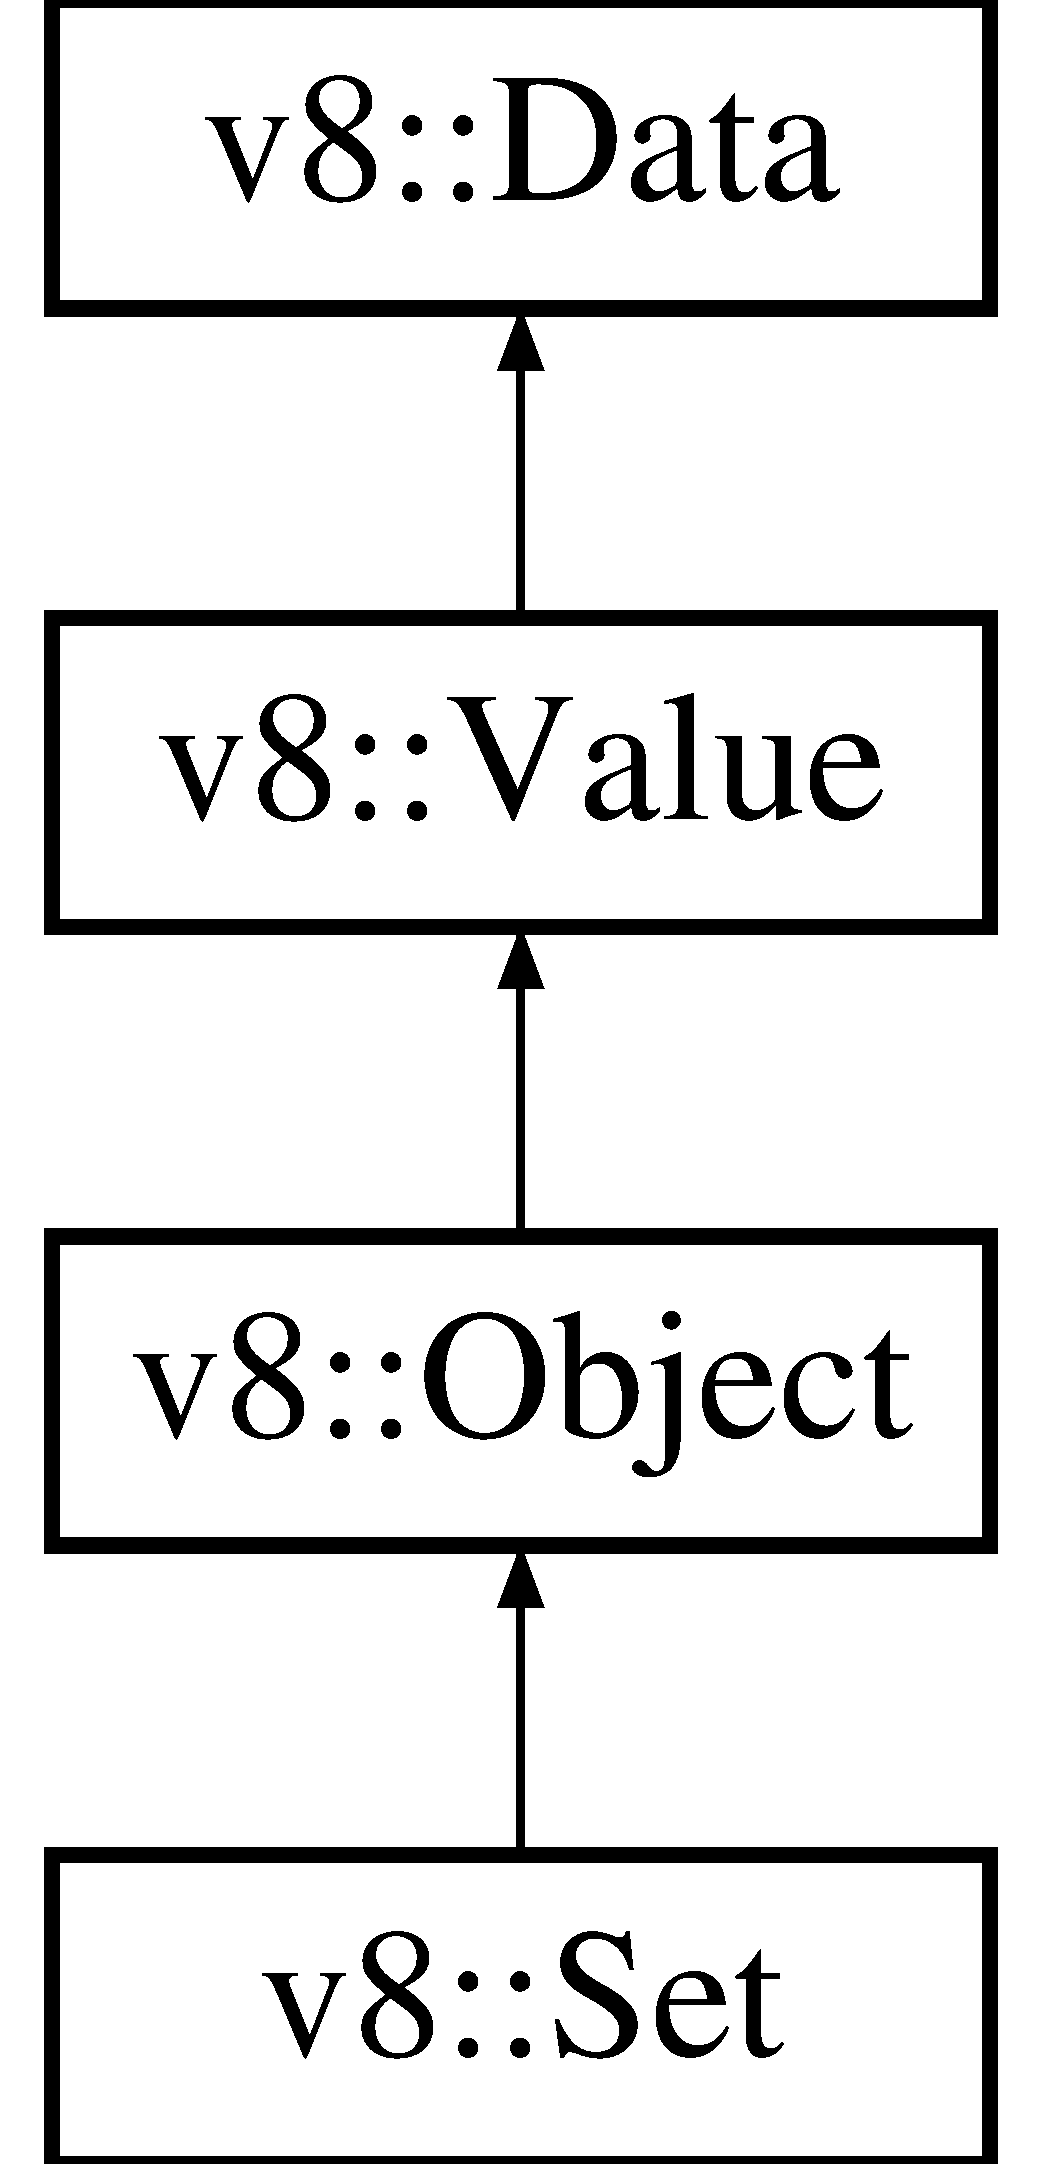
\includegraphics[height=4.000000cm]{classv8_1_1Set}
\end{center}
\end{figure}
\subsection*{Public Member Functions}
\begin{DoxyCompactItemize}
\item 
\mbox{\Hypertarget{classv8_1_1Set_af44475aaf38b9429e129d62c34bcc024}\label{classv8_1_1Set_af44475aaf38b9429e129d62c34bcc024}} 
size\+\_\+t {\bfseries Size} () const
\item 
\mbox{\Hypertarget{classv8_1_1Set_a5f7e4dbd6729a503ca617415d5eeedf0}\label{classv8_1_1Set_a5f7e4dbd6729a503ca617415d5eeedf0}} 
void {\bfseries Clear} ()
\item 
\mbox{\Hypertarget{classv8_1_1Set_adb56ad9dfa7541746b7894c359095801}\label{classv8_1_1Set_adb56ad9dfa7541746b7894c359095801}} 
V8\+\_\+\+W\+A\+R\+N\+\_\+\+U\+N\+U\+S\+E\+D\+\_\+\+R\+E\+S\+U\+LT \mbox{\hyperlink{classv8_1_1MaybeLocal}{Maybe\+Local}}$<$ \mbox{\hyperlink{classv8_1_1Set}{Set}} $>$ {\bfseries Add} (\mbox{\hyperlink{classv8_1_1Local}{Local}}$<$ Context $>$ context, \mbox{\hyperlink{classv8_1_1Local}{Local}}$<$ \mbox{\hyperlink{classv8_1_1Value}{Value}} $>$ key)
\item 
\mbox{\Hypertarget{classv8_1_1Set_a45a2c9e7b69d7bc7e94521d1ebfcce1d}\label{classv8_1_1Set_a45a2c9e7b69d7bc7e94521d1ebfcce1d}} 
V8\+\_\+\+W\+A\+R\+N\+\_\+\+U\+N\+U\+S\+E\+D\+\_\+\+R\+E\+S\+U\+LT \mbox{\hyperlink{classv8_1_1Maybe}{Maybe}}$<$ bool $>$ {\bfseries Has} (\mbox{\hyperlink{classv8_1_1Local}{Local}}$<$ Context $>$ context, \mbox{\hyperlink{classv8_1_1Local}{Local}}$<$ \mbox{\hyperlink{classv8_1_1Value}{Value}} $>$ key)
\item 
\mbox{\Hypertarget{classv8_1_1Set_a638909072ad2de7fe0e207e4889ea9bf}\label{classv8_1_1Set_a638909072ad2de7fe0e207e4889ea9bf}} 
V8\+\_\+\+W\+A\+R\+N\+\_\+\+U\+N\+U\+S\+E\+D\+\_\+\+R\+E\+S\+U\+LT \mbox{\hyperlink{classv8_1_1Maybe}{Maybe}}$<$ bool $>$ {\bfseries Delete} (\mbox{\hyperlink{classv8_1_1Local}{Local}}$<$ Context $>$ context, \mbox{\hyperlink{classv8_1_1Local}{Local}}$<$ \mbox{\hyperlink{classv8_1_1Value}{Value}} $>$ key)
\item 
\mbox{\hyperlink{classv8_1_1Local}{Local}}$<$ \mbox{\hyperlink{classv8_1_1Array}{Array}} $>$ \mbox{\hyperlink{classv8_1_1Set_aa4e8576e0a657bcd61364f3bc26e2b56}{As\+Array}} () const
\end{DoxyCompactItemize}
\subsection*{Static Public Member Functions}
\begin{DoxyCompactItemize}
\item 
static \mbox{\hyperlink{classv8_1_1Local}{Local}}$<$ \mbox{\hyperlink{classv8_1_1Set}{Set}} $>$ \mbox{\hyperlink{classv8_1_1Set_a036e773566a36997a79e78ef0a4103a1}{New}} (Isolate $\ast$isolate)
\item 
\mbox{\Hypertarget{classv8_1_1Set_a1739da4ee6bf39c381b83023f653e995}\label{classv8_1_1Set_a1739da4ee6bf39c381b83023f653e995}} 
static V8\+\_\+\+I\+N\+L\+I\+NE \mbox{\hyperlink{classv8_1_1Set}{Set}} $\ast$ {\bfseries Cast} (\mbox{\hyperlink{classv8_1_1Value}{Value}} $\ast$obj)
\end{DoxyCompactItemize}


\subsection{Detailed Description}
An instance of the built-\/in \mbox{\hyperlink{classv8_1_1Set}{Set}} constructor (E\+C\+M\+A-\/262, 6th Edition, 23.\+2.\+1). 

Definition at line 3740 of file v8.\+h.



\subsection{Member Function Documentation}
\mbox{\Hypertarget{classv8_1_1Set_aa4e8576e0a657bcd61364f3bc26e2b56}\label{classv8_1_1Set_aa4e8576e0a657bcd61364f3bc26e2b56}} 
\index{v8\+::\+Set@{v8\+::\+Set}!As\+Array@{As\+Array}}
\index{As\+Array@{As\+Array}!v8\+::\+Set@{v8\+::\+Set}}
\subsubsection{\texorpdfstring{As\+Array()}{AsArray()}}
{\footnotesize\ttfamily \mbox{\hyperlink{classv8_1_1Local}{Local}}$<$\mbox{\hyperlink{classv8_1_1Array}{Array}}$>$ v8\+::\+Set\+::\+As\+Array (\begin{DoxyParamCaption}{ }\end{DoxyParamCaption}) const}

Returns an array of the keys in this \mbox{\hyperlink{classv8_1_1Set}{Set}}. \mbox{\Hypertarget{classv8_1_1Set_a036e773566a36997a79e78ef0a4103a1}\label{classv8_1_1Set_a036e773566a36997a79e78ef0a4103a1}} 
\index{v8\+::\+Set@{v8\+::\+Set}!New@{New}}
\index{New@{New}!v8\+::\+Set@{v8\+::\+Set}}
\subsubsection{\texorpdfstring{New()}{New()}}
{\footnotesize\ttfamily static \mbox{\hyperlink{classv8_1_1Local}{Local}}$<$\mbox{\hyperlink{classv8_1_1Set}{Set}}$>$ v8\+::\+Set\+::\+New (\begin{DoxyParamCaption}\item[{Isolate $\ast$}]{isolate }\end{DoxyParamCaption})\hspace{0.3cm}{\ttfamily [static]}}

Creates a new empty \mbox{\hyperlink{classv8_1_1Set}{Set}}. 

The documentation for this class was generated from the following file\+:\begin{DoxyCompactItemize}
\item 
v8/include/v8.\+h\end{DoxyCompactItemize}

\hypertarget{classv8_1_1SharedArrayBuffer}{}\section{v8\+:\+:Shared\+Array\+Buffer Class Reference}
\label{classv8_1_1SharedArrayBuffer}\index{v8\+::\+Shared\+Array\+Buffer@{v8\+::\+Shared\+Array\+Buffer}}


{\ttfamily \#include $<$v8.\+h$>$}

Inheritance diagram for v8\+:\+:Shared\+Array\+Buffer\+:\begin{figure}[H]
\begin{center}
\leavevmode
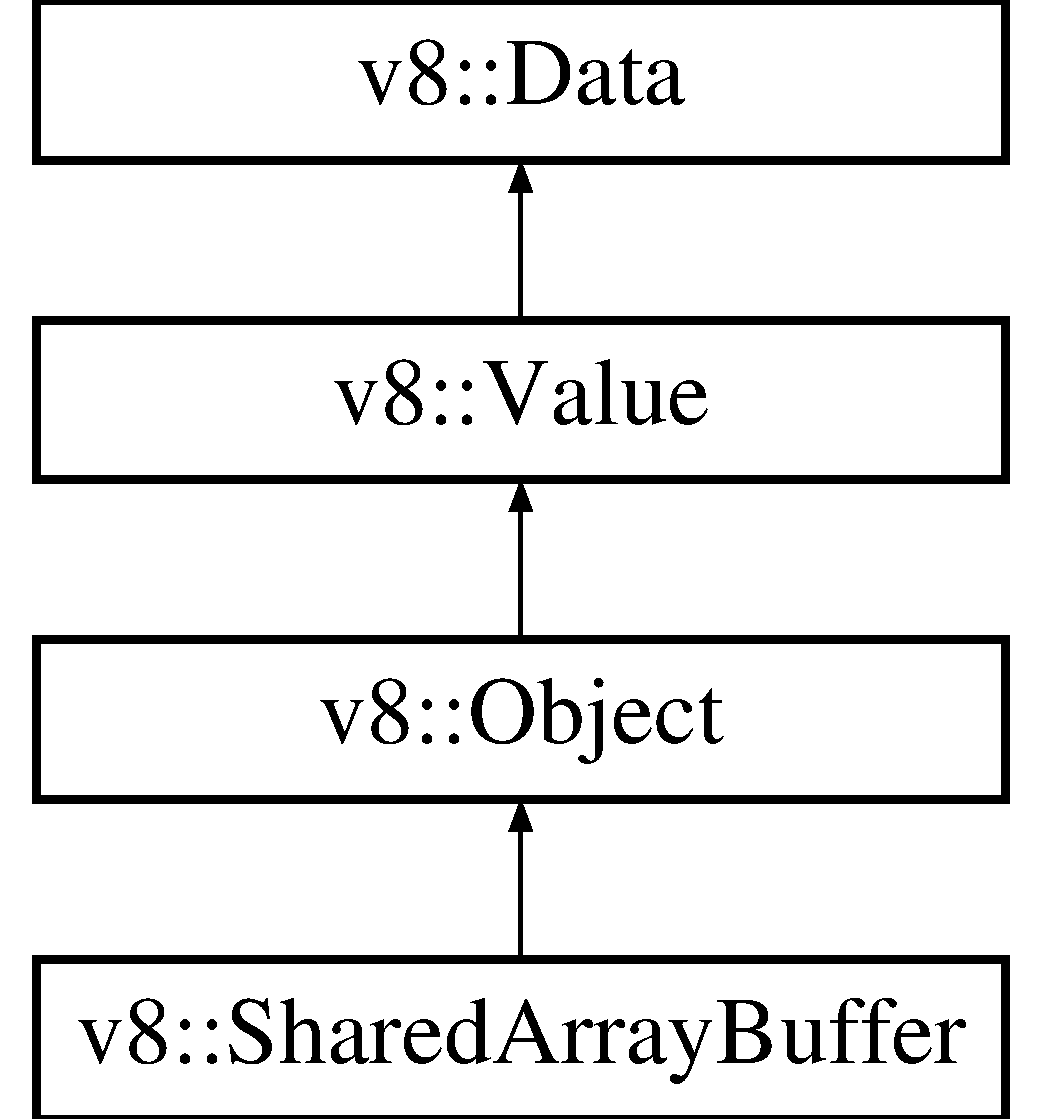
\includegraphics[height=4.000000cm]{classv8_1_1SharedArrayBuffer}
\end{center}
\end{figure}
\subsection*{Data Structures}
\begin{DoxyCompactItemize}
\item 
class \hyperlink{classv8_1_1SharedArrayBuffer_1_1Contents}{Contents}
\end{DoxyCompactItemize}
\subsection*{Public Member Functions}
\begin{DoxyCompactItemize}
\item 
size\+\_\+t \hyperlink{classv8_1_1SharedArrayBuffer_a09cfb461e2f3f8e1fca53a4a2fbfd8df}{Byte\+Length} () const 
\item 
bool \hyperlink{classv8_1_1SharedArrayBuffer_a37e7ba1ed5a1422af9928697ea6a960b}{Is\+External} () const 
\item 
\hyperlink{classv8_1_1SharedArrayBuffer_1_1Contents}{Contents} \hyperlink{classv8_1_1SharedArrayBuffer_afe025bbf668e64439cfc0044b353eb41}{Externalize} ()
\item 
\hyperlink{classv8_1_1SharedArrayBuffer_1_1Contents}{Contents} \hyperlink{classv8_1_1SharedArrayBuffer_af5a160b645c5c674450d9501697c2cf4}{Get\+Contents} ()
\end{DoxyCompactItemize}
\subsection*{Static Public Member Functions}
\begin{DoxyCompactItemize}
\item 
static \hyperlink{classv8_1_1Local}{Local}$<$ \hyperlink{classv8_1_1SharedArrayBuffer}{Shared\+Array\+Buffer} $>$ \hyperlink{classv8_1_1SharedArrayBuffer_a0e7060cc31105c5bf780d770c1a7acc6}{New} (\hyperlink{classv8_1_1Isolate}{Isolate} $\ast$isolate, size\+\_\+t byte\+\_\+length)
\item 
static \hyperlink{classv8_1_1Local}{Local}$<$ \hyperlink{classv8_1_1SharedArrayBuffer}{Shared\+Array\+Buffer} $>$ \hyperlink{classv8_1_1SharedArrayBuffer_af708b1765380ad42b7d572dfc531c21c}{New} (\hyperlink{classv8_1_1Isolate}{Isolate} $\ast$isolate, void $\ast$data, size\+\_\+t byte\+\_\+length, Array\+Buffer\+Creation\+Mode mode=Array\+Buffer\+Creation\+Mode\+::k\+Externalized)
\item 
static V8\+\_\+\+I\+N\+L\+I\+NE \hyperlink{classv8_1_1SharedArrayBuffer}{Shared\+Array\+Buffer} $\ast$ {\bfseries Cast} (\hyperlink{classv8_1_1Value}{Value} $\ast$obj)\hypertarget{classv8_1_1SharedArrayBuffer_ac4e1ba5d4564c7033814f4cc45fdda84}{}\label{classv8_1_1SharedArrayBuffer_ac4e1ba5d4564c7033814f4cc45fdda84}

\end{DoxyCompactItemize}
\subsection*{Static Public Attributes}
\begin{DoxyCompactItemize}
\item 
static const int {\bfseries k\+Internal\+Field\+Count} = V8\+\_\+\+A\+R\+R\+A\+Y\+\_\+\+B\+U\+F\+F\+E\+R\+\_\+\+I\+N\+T\+E\+R\+N\+A\+L\+\_\+\+F\+I\+E\+L\+D\+\_\+\+C\+O\+U\+NT\hypertarget{classv8_1_1SharedArrayBuffer_a6f47f6b441e37aefd1a9d0176e8a3da8}{}\label{classv8_1_1SharedArrayBuffer_a6f47f6b441e37aefd1a9d0176e8a3da8}

\end{DoxyCompactItemize}


\subsection{Detailed Description}
An instance of the built-\/in \hyperlink{classv8_1_1SharedArrayBuffer}{Shared\+Array\+Buffer} constructor. This A\+PI is experimental and may change significantly. 

\subsection{Member Function Documentation}
\index{v8\+::\+Shared\+Array\+Buffer@{v8\+::\+Shared\+Array\+Buffer}!Byte\+Length@{Byte\+Length}}
\index{Byte\+Length@{Byte\+Length}!v8\+::\+Shared\+Array\+Buffer@{v8\+::\+Shared\+Array\+Buffer}}
\subsubsection[{\texorpdfstring{Byte\+Length() const }{ByteLength() const }}]{\setlength{\rightskip}{0pt plus 5cm}size\+\_\+t v8\+::\+Shared\+Array\+Buffer\+::\+Byte\+Length (
\begin{DoxyParamCaption}
{}
\end{DoxyParamCaption}
) const}\hypertarget{classv8_1_1SharedArrayBuffer_a09cfb461e2f3f8e1fca53a4a2fbfd8df}{}\label{classv8_1_1SharedArrayBuffer_a09cfb461e2f3f8e1fca53a4a2fbfd8df}
\hyperlink{classv8_1_1Data}{Data} length in bytes. \index{v8\+::\+Shared\+Array\+Buffer@{v8\+::\+Shared\+Array\+Buffer}!Externalize@{Externalize}}
\index{Externalize@{Externalize}!v8\+::\+Shared\+Array\+Buffer@{v8\+::\+Shared\+Array\+Buffer}}
\subsubsection[{\texorpdfstring{Externalize()}{Externalize()}}]{\setlength{\rightskip}{0pt plus 5cm}{\bf Contents} v8\+::\+Shared\+Array\+Buffer\+::\+Externalize (
\begin{DoxyParamCaption}
{}
\end{DoxyParamCaption}
)}\hypertarget{classv8_1_1SharedArrayBuffer_afe025bbf668e64439cfc0044b353eb41}{}\label{classv8_1_1SharedArrayBuffer_afe025bbf668e64439cfc0044b353eb41}
Make this \hyperlink{classv8_1_1SharedArrayBuffer}{Shared\+Array\+Buffer} external. The pointer to underlying memory block and byte length are returned as $\vert$\+Contents$\vert$ structure. After \hyperlink{classv8_1_1SharedArrayBuffer}{Shared\+Array\+Buffer} had been etxrenalized, it does no longer owns the memory block. The caller should take steps to free memory when it is no longer needed.

The memory block is guaranteed to be allocated with $\vert$\+Allocator\+::\+Allocate$\vert$ by the allocator specified in \hyperlink{structv8_1_1Isolate_1_1CreateParams_a7c663f70b64290392eeaf164f57585f9}{v8\+::\+Isolate\+::\+Create\+Params\+::array\+\_\+buffer\+\_\+allocator}. \index{v8\+::\+Shared\+Array\+Buffer@{v8\+::\+Shared\+Array\+Buffer}!Get\+Contents@{Get\+Contents}}
\index{Get\+Contents@{Get\+Contents}!v8\+::\+Shared\+Array\+Buffer@{v8\+::\+Shared\+Array\+Buffer}}
\subsubsection[{\texorpdfstring{Get\+Contents()}{GetContents()}}]{\setlength{\rightskip}{0pt plus 5cm}{\bf Contents} v8\+::\+Shared\+Array\+Buffer\+::\+Get\+Contents (
\begin{DoxyParamCaption}
{}
\end{DoxyParamCaption}
)}\hypertarget{classv8_1_1SharedArrayBuffer_af5a160b645c5c674450d9501697c2cf4}{}\label{classv8_1_1SharedArrayBuffer_af5a160b645c5c674450d9501697c2cf4}
Get a pointer to the \hyperlink{classv8_1_1ArrayBuffer}{Array\+Buffer}\textquotesingle{}s underlying memory block without externalizing it. If the \hyperlink{classv8_1_1ArrayBuffer}{Array\+Buffer} is not externalized, this pointer will become invalid as soon as the \hyperlink{classv8_1_1ArrayBuffer}{Array\+Buffer} became garbage collected.

The embedder should make sure to hold a strong reference to the \hyperlink{classv8_1_1ArrayBuffer}{Array\+Buffer} while accessing this pointer.

The memory block is guaranteed to be allocated with $\vert$\+Allocator\+::\+Allocate$\vert$ by the allocator specified in \hyperlink{structv8_1_1Isolate_1_1CreateParams_a7c663f70b64290392eeaf164f57585f9}{v8\+::\+Isolate\+::\+Create\+Params\+::array\+\_\+buffer\+\_\+allocator}. \index{v8\+::\+Shared\+Array\+Buffer@{v8\+::\+Shared\+Array\+Buffer}!Is\+External@{Is\+External}}
\index{Is\+External@{Is\+External}!v8\+::\+Shared\+Array\+Buffer@{v8\+::\+Shared\+Array\+Buffer}}
\subsubsection[{\texorpdfstring{Is\+External() const }{IsExternal() const }}]{\setlength{\rightskip}{0pt plus 5cm}bool v8\+::\+Shared\+Array\+Buffer\+::\+Is\+External (
\begin{DoxyParamCaption}
{}
\end{DoxyParamCaption}
) const}\hypertarget{classv8_1_1SharedArrayBuffer_a37e7ba1ed5a1422af9928697ea6a960b}{}\label{classv8_1_1SharedArrayBuffer_a37e7ba1ed5a1422af9928697ea6a960b}
Returns true if \hyperlink{classv8_1_1SharedArrayBuffer}{Shared\+Array\+Buffer} is externalized, that is, does not own its memory block. \index{v8\+::\+Shared\+Array\+Buffer@{v8\+::\+Shared\+Array\+Buffer}!New@{New}}
\index{New@{New}!v8\+::\+Shared\+Array\+Buffer@{v8\+::\+Shared\+Array\+Buffer}}
\subsubsection[{\texorpdfstring{New(\+Isolate $\ast$isolate, size\+\_\+t byte\+\_\+length)}{New(Isolate *isolate, size_t byte_length)}}]{\setlength{\rightskip}{0pt plus 5cm}static {\bf Local}$<${\bf Shared\+Array\+Buffer}$>$ v8\+::\+Shared\+Array\+Buffer\+::\+New (
\begin{DoxyParamCaption}
\item[{{\bf Isolate} $\ast$}]{isolate, }
\item[{size\+\_\+t}]{byte\+\_\+length}
\end{DoxyParamCaption}
)\hspace{0.3cm}{\ttfamily [static]}}\hypertarget{classv8_1_1SharedArrayBuffer_a0e7060cc31105c5bf780d770c1a7acc6}{}\label{classv8_1_1SharedArrayBuffer_a0e7060cc31105c5bf780d770c1a7acc6}
Create a new \hyperlink{classv8_1_1SharedArrayBuffer}{Shared\+Array\+Buffer}. Allocate $\vert$byte\+\_\+length$\vert$ bytes. Allocated memory will be owned by a created \hyperlink{classv8_1_1SharedArrayBuffer}{Shared\+Array\+Buffer} and will be deallocated when it is garbage-\/collected, unless the object is externalized. \index{v8\+::\+Shared\+Array\+Buffer@{v8\+::\+Shared\+Array\+Buffer}!New@{New}}
\index{New@{New}!v8\+::\+Shared\+Array\+Buffer@{v8\+::\+Shared\+Array\+Buffer}}
\subsubsection[{\texorpdfstring{New(\+Isolate $\ast$isolate, void $\ast$data, size\+\_\+t byte\+\_\+length, Array\+Buffer\+Creation\+Mode mode=\+Array\+Buffer\+Creation\+Mode\+::k\+Externalized)}{New(Isolate *isolate, void *data, size_t byte_length, ArrayBufferCreationMode mode=ArrayBufferCreationMode::kExternalized)}}]{\setlength{\rightskip}{0pt plus 5cm}static {\bf Local}$<${\bf Shared\+Array\+Buffer}$>$ v8\+::\+Shared\+Array\+Buffer\+::\+New (
\begin{DoxyParamCaption}
\item[{{\bf Isolate} $\ast$}]{isolate, }
\item[{void $\ast$}]{data, }
\item[{size\+\_\+t}]{byte\+\_\+length, }
\item[{Array\+Buffer\+Creation\+Mode}]{mode = {\ttfamily ArrayBufferCreationMode\+:\+:kExternalized}}
\end{DoxyParamCaption}
)\hspace{0.3cm}{\ttfamily [static]}}\hypertarget{classv8_1_1SharedArrayBuffer_af708b1765380ad42b7d572dfc531c21c}{}\label{classv8_1_1SharedArrayBuffer_af708b1765380ad42b7d572dfc531c21c}
Create a new \hyperlink{classv8_1_1SharedArrayBuffer}{Shared\+Array\+Buffer} over an existing memory block. The created array buffer is immediately in externalized state unless otherwise specified. The memory block will not be reclaimed when a created \hyperlink{classv8_1_1SharedArrayBuffer}{Shared\+Array\+Buffer} is garbage-\/collected. 

The documentation for this class was generated from the following file\+:\begin{DoxyCompactItemize}
\item 
v8/include/v8.\+h\end{DoxyCompactItemize}

\hypertarget{classv8_1_1Signature}{}\section{v8\+:\+:Signature Class Reference}
\label{classv8_1_1Signature}\index{v8\+::\+Signature@{v8\+::\+Signature}}


{\ttfamily \#include $<$v8.\+h$>$}

Inheritance diagram for v8\+:\+:Signature\+:\begin{figure}[H]
\begin{center}
\leavevmode
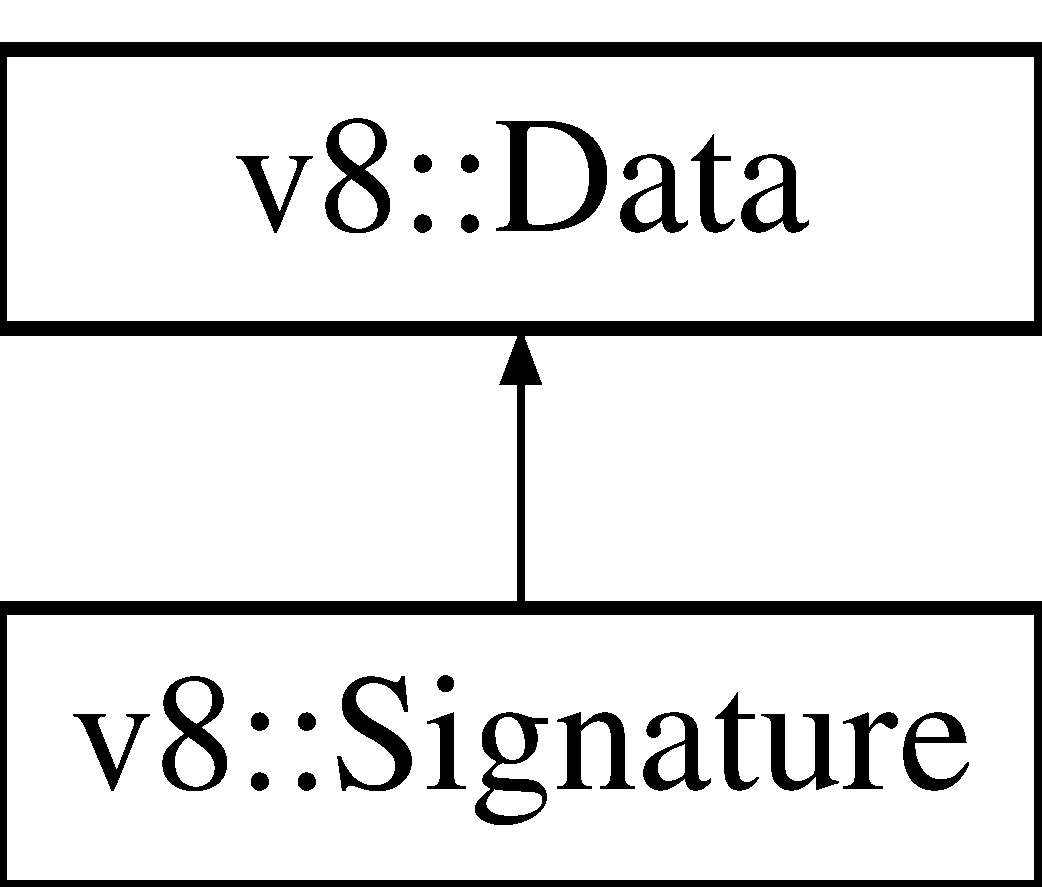
\includegraphics[height=2.000000cm]{classv8_1_1Signature}
\end{center}
\end{figure}
\subsection*{Static Public Member Functions}
\begin{DoxyCompactItemize}
\item 
\mbox{\Hypertarget{classv8_1_1Signature_a4e3d622674ec1f735e9981ec3309320f}\label{classv8_1_1Signature_a4e3d622674ec1f735e9981ec3309320f}} 
static \mbox{\hyperlink{classv8_1_1Local}{Local}}$<$ \mbox{\hyperlink{classv8_1_1Signature}{Signature}} $>$ {\bfseries New} (Isolate $\ast$isolate, \mbox{\hyperlink{classv8_1_1Local}{Local}}$<$ \mbox{\hyperlink{classv8_1_1FunctionTemplate}{Function\+Template}} $>$ receiver=\mbox{\hyperlink{classv8_1_1Local}{Local}}$<$ \mbox{\hyperlink{classv8_1_1FunctionTemplate}{Function\+Template}} $>$())
\item 
\mbox{\Hypertarget{classv8_1_1Signature_a9c7566555923187ca55c14af8048a9fc}\label{classv8_1_1Signature_a9c7566555923187ca55c14af8048a9fc}} 
static V8\+\_\+\+I\+N\+L\+I\+NE \mbox{\hyperlink{classv8_1_1Signature}{Signature}} $\ast$ {\bfseries Cast} (\mbox{\hyperlink{classv8_1_1Data}{Data}} $\ast$data)
\end{DoxyCompactItemize}


\subsection{Detailed Description}
A \mbox{\hyperlink{classv8_1_1Signature}{Signature}} specifies which receiver is valid for a function.

A receiver matches a given signature if the receiver (or any of its hidden prototypes) was created from the signature\textquotesingle{}s \mbox{\hyperlink{classv8_1_1FunctionTemplate}{Function\+Template}}, or from a \mbox{\hyperlink{classv8_1_1FunctionTemplate}{Function\+Template}} that inherits directly or indirectly from the signature\textquotesingle{}s \mbox{\hyperlink{classv8_1_1FunctionTemplate}{Function\+Template}}. 

The documentation for this class was generated from the following file\+:\begin{DoxyCompactItemize}
\item 
v8/include/v8.\+h\end{DoxyCompactItemize}

\hypertarget{structv8_1_1internal_1_1SmiTagging}{}\section{v8\+:\+:internal\+:\+:Smi\+Tagging$<$ tagged\+\_\+ptr\+\_\+size $>$ Struct Template Reference}
\label{structv8_1_1internal_1_1SmiTagging}\index{v8\+::internal\+::\+Smi\+Tagging$<$ tagged\+\_\+ptr\+\_\+size $>$@{v8\+::internal\+::\+Smi\+Tagging$<$ tagged\+\_\+ptr\+\_\+size $>$}}


\subsection{Detailed Description}
\subsubsection*{template$<$size\+\_\+t tagged\+\_\+ptr\+\_\+size$>$\newline
struct v8\+::internal\+::\+Smi\+Tagging$<$ tagged\+\_\+ptr\+\_\+size $>$}



Definition at line 47 of file v8-\/internal.\+h.



The documentation for this struct was generated from the following file\+:\begin{DoxyCompactItemize}
\item 
v8/include/v8-\/internal.\+h\end{DoxyCompactItemize}

\hypertarget{structv8_1_1internal_1_1SmiTagging_3_014_01_4}{}\section{v8\+:\+:internal\+:\+:Smi\+Tagging$<$ 4 $>$ Struct Template Reference}
\label{structv8_1_1internal_1_1SmiTagging_3_014_01_4}\index{v8\+::internal\+::\+Smi\+Tagging$<$ 4 $>$@{v8\+::internal\+::\+Smi\+Tagging$<$ 4 $>$}}
\subsection*{Public Types}
\begin{DoxyCompactItemize}
\item 
\mbox{\Hypertarget{structv8_1_1internal_1_1SmiTagging_3_014_01_4_aa2b64cedd7f894f6964fe11746b029e4}\label{structv8_1_1internal_1_1SmiTagging_3_014_01_4_aa2b64cedd7f894f6964fe11746b029e4}} 
enum \{ {\bfseries k\+Smi\+Shift\+Size} = 0, 
{\bfseries k\+Smi\+Value\+Size} = 31
 \}
\end{DoxyCompactItemize}
\subsection*{Static Public Member Functions}
\begin{DoxyCompactItemize}
\item 
\mbox{\Hypertarget{structv8_1_1internal_1_1SmiTagging_3_014_01_4_ad306fdee17af069303cc78be3defa400}\label{structv8_1_1internal_1_1SmiTagging_3_014_01_4_ad306fdee17af069303cc78be3defa400}} 
static V8\+\_\+\+I\+N\+L\+I\+NE int {\bfseries Smi\+To\+Int} (const internal\+::\+Address value)
\item 
\mbox{\Hypertarget{structv8_1_1internal_1_1SmiTagging_3_014_01_4_af100af8e269bbeee8c7e12b28d388b4e}\label{structv8_1_1internal_1_1SmiTagging_3_014_01_4_af100af8e269bbeee8c7e12b28d388b4e}} 
static V8\+\_\+\+I\+N\+L\+I\+NE constexpr bool {\bfseries Is\+Valid\+Smi} (intptr\+\_\+t value)
\end{DoxyCompactItemize}


The documentation for this struct was generated from the following file\+:\begin{DoxyCompactItemize}
\item 
v8/include/v8-\/internal.\+h\end{DoxyCompactItemize}

\hypertarget{structv8_1_1internal_1_1SmiTagging_3_018_01_4}{}\section{v8\+:\+:internal\+:\+:Smi\+Tagging$<$ 8 $>$ Struct Template Reference}
\label{structv8_1_1internal_1_1SmiTagging_3_018_01_4}\index{v8\+::internal\+::\+Smi\+Tagging$<$ 8 $>$@{v8\+::internal\+::\+Smi\+Tagging$<$ 8 $>$}}
\subsection*{Public Types}
\begin{DoxyCompactItemize}
\item 
\hypertarget{structv8_1_1internal_1_1SmiTagging_3_018_01_4_aca1e57809e36a53b790ee0480324fb7b}{}enum \{ {\bfseries k\+Smi\+Shift\+Size} = 31, 
{\bfseries k\+Smi\+Value\+Size} = 32
 \}\label{structv8_1_1internal_1_1SmiTagging_3_018_01_4_aca1e57809e36a53b790ee0480324fb7b}

\end{DoxyCompactItemize}
\subsection*{Static Public Member Functions}
\begin{DoxyCompactItemize}
\item 
\hypertarget{structv8_1_1internal_1_1SmiTagging_3_018_01_4_a4fb28f586fdee8316a03f9b8f94b945d}{}static int {\bfseries Smi\+Shift\+Size} ()\label{structv8_1_1internal_1_1SmiTagging_3_018_01_4_a4fb28f586fdee8316a03f9b8f94b945d}

\item 
\hypertarget{structv8_1_1internal_1_1SmiTagging_3_018_01_4_a836e783af92beb7ca9cc8cdabef43ab2}{}static int {\bfseries Smi\+Value\+Size} ()\label{structv8_1_1internal_1_1SmiTagging_3_018_01_4_a836e783af92beb7ca9cc8cdabef43ab2}

\item 
\hypertarget{structv8_1_1internal_1_1SmiTagging_3_018_01_4_a040db1ceee3195c2463075b7b50cfda0}{}static V8\+\_\+\+I\+N\+L\+I\+N\+E int {\bfseries Smi\+To\+Int} (const internal\+::\+Object $\ast$value)\label{structv8_1_1internal_1_1SmiTagging_3_018_01_4_a040db1ceee3195c2463075b7b50cfda0}

\item 
\hypertarget{structv8_1_1internal_1_1SmiTagging_3_018_01_4_a1926f38e35fc98fe244e8136180d70f2}{}static V8\+\_\+\+I\+N\+L\+I\+N\+E internal\+::\+Object $\ast$ {\bfseries Int\+To\+Smi} (int value)\label{structv8_1_1internal_1_1SmiTagging_3_018_01_4_a1926f38e35fc98fe244e8136180d70f2}

\item 
\hypertarget{structv8_1_1internal_1_1SmiTagging_3_018_01_4_a5ab93d4cf7c3b9ceff5116b3598a1f94}{}static V8\+\_\+\+I\+N\+L\+I\+N\+E bool {\bfseries Is\+Valid\+Smi} (intptr\+\_\+t value)\label{structv8_1_1internal_1_1SmiTagging_3_018_01_4_a5ab93d4cf7c3b9ceff5116b3598a1f94}

\end{DoxyCompactItemize}


The documentation for this struct was generated from the following file\+:\begin{DoxyCompactItemize}
\item 
v8/include/v8.\+h\end{DoxyCompactItemize}

\hypertarget{classv8_1_1ScriptCompiler_1_1Source}{}\section{v8\+:\+:Script\+Compiler\+:\+:Source Class Reference}
\label{classv8_1_1ScriptCompiler_1_1Source}\index{v8\+::\+Script\+Compiler\+::\+Source@{v8\+::\+Script\+Compiler\+::\+Source}}


{\ttfamily \#include $<$v8.\+h$>$}

\subsection*{Public Member Functions}
\begin{DoxyCompactItemize}
\item 
V8\+\_\+\+I\+N\+L\+I\+NE {\bfseries Source} (\hyperlink{classv8_1_1Local}{Local}$<$ \hyperlink{classv8_1_1String}{String} $>$ source\+\_\+string, const \hyperlink{classv8_1_1ScriptOrigin}{Script\+Origin} \&origin, \hyperlink{structv8_1_1ScriptCompiler_1_1CachedData}{Cached\+Data} $\ast$cached\+\_\+data=N\+U\+LL)\hypertarget{classv8_1_1ScriptCompiler_1_1Source_ae71a5fe18124d71f9acfcc872310d586}{}\label{classv8_1_1ScriptCompiler_1_1Source_ae71a5fe18124d71f9acfcc872310d586}

\item 
V8\+\_\+\+I\+N\+L\+I\+NE {\bfseries Source} (\hyperlink{classv8_1_1Local}{Local}$<$ \hyperlink{classv8_1_1String}{String} $>$ source\+\_\+string, \hyperlink{structv8_1_1ScriptCompiler_1_1CachedData}{Cached\+Data} $\ast$cached\+\_\+data=N\+U\+LL)\hypertarget{classv8_1_1ScriptCompiler_1_1Source_ad46e9d298cf3199c3a570182a680449d}{}\label{classv8_1_1ScriptCompiler_1_1Source_ad46e9d298cf3199c3a570182a680449d}

\item 
V8\+\_\+\+I\+N\+L\+I\+NE const \hyperlink{structv8_1_1ScriptCompiler_1_1CachedData}{Cached\+Data} $\ast$ {\bfseries Get\+Cached\+Data} () const \hypertarget{classv8_1_1ScriptCompiler_1_1Source_a7cef3113a46627fefa3110132acf47d2}{}\label{classv8_1_1ScriptCompiler_1_1Source_a7cef3113a46627fefa3110132acf47d2}

\end{DoxyCompactItemize}
\subsection*{Friends}
\begin{DoxyCompactItemize}
\item 
class {\bfseries Script\+Compiler}\hypertarget{classv8_1_1ScriptCompiler_1_1Source_a1cb50af99960b4c11eaee7347e034f51}{}\label{classv8_1_1ScriptCompiler_1_1Source_a1cb50af99960b4c11eaee7347e034f51}

\end{DoxyCompactItemize}


\subsection{Detailed Description}
\hyperlink{classv8_1_1ScriptCompiler_1_1Source}{Source} code which can be then compiled to a \hyperlink{classv8_1_1UnboundScript}{Unbound\+Script} or \hyperlink{classv8_1_1Script}{Script}. 

The documentation for this class was generated from the following file\+:\begin{DoxyCompactItemize}
\item 
v8/include/v8.\+h\end{DoxyCompactItemize}

\hypertarget{classv8_1_1StackFrame}{}\section{v8\+:\+:Stack\+Frame Class Reference}
\label{classv8_1_1StackFrame}\index{v8\+::\+Stack\+Frame@{v8\+::\+Stack\+Frame}}


{\ttfamily \#include $<$v8.\+h$>$}

\subsection*{Public Member Functions}
\begin{DoxyCompactItemize}
\item 
int \mbox{\hyperlink{classv8_1_1StackFrame_a34ab9f48a06525cd9f93e01a70427ca2}{Get\+Line\+Number}} () const
\item 
int \mbox{\hyperlink{classv8_1_1StackFrame_a3b4d7d29ae82b88304d09ea5c5e43db1}{Get\+Column}} () const
\item 
int \mbox{\hyperlink{classv8_1_1StackFrame_ac2f0f26b9c7aee860cdd613c0d83ae35}{Get\+Script\+Id}} () const
\item 
\mbox{\hyperlink{classv8_1_1Local}{Local}}$<$ \mbox{\hyperlink{classv8_1_1String}{String}} $>$ \mbox{\hyperlink{classv8_1_1StackFrame_a2885f14557e14c64396206b0f79daa3e}{Get\+Script\+Name}} () const
\item 
\mbox{\hyperlink{classv8_1_1Local}{Local}}$<$ \mbox{\hyperlink{classv8_1_1String}{String}} $>$ \mbox{\hyperlink{classv8_1_1StackFrame_a4fbd286090b13661b3db148e0a3779b5}{Get\+Script\+Name\+Or\+Source\+U\+RL}} () const
\item 
\mbox{\hyperlink{classv8_1_1Local}{Local}}$<$ \mbox{\hyperlink{classv8_1_1String}{String}} $>$ \mbox{\hyperlink{classv8_1_1StackFrame_a9cd783598db74ab35bd4ae7c8cbc374f}{Get\+Function\+Name}} () const
\item 
bool \mbox{\hyperlink{classv8_1_1StackFrame_aa07e67a6a00adcd0f5c8c4ba7a82e54a}{Is\+Eval}} () const
\item 
bool \mbox{\hyperlink{classv8_1_1StackFrame_a8f37df38214b6dc10655fc50f0341eb8}{Is\+Constructor}} () const
\item 
bool \mbox{\hyperlink{classv8_1_1StackFrame_aec6d28360828b8cadc3da6a5dbd83d89}{Is\+Wasm}} () const
\end{DoxyCompactItemize}


\subsection{Detailed Description}
A single Java\+Script stack frame. 

\subsection{Member Function Documentation}
\mbox{\Hypertarget{classv8_1_1StackFrame_a3b4d7d29ae82b88304d09ea5c5e43db1}\label{classv8_1_1StackFrame_a3b4d7d29ae82b88304d09ea5c5e43db1}} 
\index{v8\+::\+Stack\+Frame@{v8\+::\+Stack\+Frame}!Get\+Column@{Get\+Column}}
\index{Get\+Column@{Get\+Column}!v8\+::\+Stack\+Frame@{v8\+::\+Stack\+Frame}}
\subsubsection{\texorpdfstring{Get\+Column()}{GetColumn()}}
{\footnotesize\ttfamily int v8\+::\+Stack\+Frame\+::\+Get\+Column (\begin{DoxyParamCaption}{ }\end{DoxyParamCaption}) const}

Returns the 1-\/based column offset on the line for the associated function call. This method will return Message\+::k\+No\+Column\+Info if it is unable to retrieve the column number, or if k\+Column\+Offset was not passed as an option when capturing the \mbox{\hyperlink{classv8_1_1StackTrace}{Stack\+Trace}}. \mbox{\Hypertarget{classv8_1_1StackFrame_a9cd783598db74ab35bd4ae7c8cbc374f}\label{classv8_1_1StackFrame_a9cd783598db74ab35bd4ae7c8cbc374f}} 
\index{v8\+::\+Stack\+Frame@{v8\+::\+Stack\+Frame}!Get\+Function\+Name@{Get\+Function\+Name}}
\index{Get\+Function\+Name@{Get\+Function\+Name}!v8\+::\+Stack\+Frame@{v8\+::\+Stack\+Frame}}
\subsubsection{\texorpdfstring{Get\+Function\+Name()}{GetFunctionName()}}
{\footnotesize\ttfamily \mbox{\hyperlink{classv8_1_1Local}{Local}}$<$\mbox{\hyperlink{classv8_1_1String}{String}}$>$ v8\+::\+Stack\+Frame\+::\+Get\+Function\+Name (\begin{DoxyParamCaption}{ }\end{DoxyParamCaption}) const}

Returns the name of the function associated with this stack frame. \mbox{\Hypertarget{classv8_1_1StackFrame_a34ab9f48a06525cd9f93e01a70427ca2}\label{classv8_1_1StackFrame_a34ab9f48a06525cd9f93e01a70427ca2}} 
\index{v8\+::\+Stack\+Frame@{v8\+::\+Stack\+Frame}!Get\+Line\+Number@{Get\+Line\+Number}}
\index{Get\+Line\+Number@{Get\+Line\+Number}!v8\+::\+Stack\+Frame@{v8\+::\+Stack\+Frame}}
\subsubsection{\texorpdfstring{Get\+Line\+Number()}{GetLineNumber()}}
{\footnotesize\ttfamily int v8\+::\+Stack\+Frame\+::\+Get\+Line\+Number (\begin{DoxyParamCaption}{ }\end{DoxyParamCaption}) const}

Returns the number, 1-\/based, of the line for the associate function call. This method will return Message\+::k\+No\+Line\+Number\+Info if it is unable to retrieve the line number, or if k\+Line\+Number was not passed as an option when capturing the \mbox{\hyperlink{classv8_1_1StackTrace}{Stack\+Trace}}. \mbox{\Hypertarget{classv8_1_1StackFrame_ac2f0f26b9c7aee860cdd613c0d83ae35}\label{classv8_1_1StackFrame_ac2f0f26b9c7aee860cdd613c0d83ae35}} 
\index{v8\+::\+Stack\+Frame@{v8\+::\+Stack\+Frame}!Get\+Script\+Id@{Get\+Script\+Id}}
\index{Get\+Script\+Id@{Get\+Script\+Id}!v8\+::\+Stack\+Frame@{v8\+::\+Stack\+Frame}}
\subsubsection{\texorpdfstring{Get\+Script\+Id()}{GetScriptId()}}
{\footnotesize\ttfamily int v8\+::\+Stack\+Frame\+::\+Get\+Script\+Id (\begin{DoxyParamCaption}{ }\end{DoxyParamCaption}) const}

Returns the id of the script for the function for this \mbox{\hyperlink{classv8_1_1StackFrame}{Stack\+Frame}}. This method will return Message\+::k\+No\+Script\+Id\+Info if it is unable to retrieve the script id, or if k\+Script\+Id was not passed as an option when capturing the \mbox{\hyperlink{classv8_1_1StackTrace}{Stack\+Trace}}. \mbox{\Hypertarget{classv8_1_1StackFrame_a2885f14557e14c64396206b0f79daa3e}\label{classv8_1_1StackFrame_a2885f14557e14c64396206b0f79daa3e}} 
\index{v8\+::\+Stack\+Frame@{v8\+::\+Stack\+Frame}!Get\+Script\+Name@{Get\+Script\+Name}}
\index{Get\+Script\+Name@{Get\+Script\+Name}!v8\+::\+Stack\+Frame@{v8\+::\+Stack\+Frame}}
\subsubsection{\texorpdfstring{Get\+Script\+Name()}{GetScriptName()}}
{\footnotesize\ttfamily \mbox{\hyperlink{classv8_1_1Local}{Local}}$<$\mbox{\hyperlink{classv8_1_1String}{String}}$>$ v8\+::\+Stack\+Frame\+::\+Get\+Script\+Name (\begin{DoxyParamCaption}{ }\end{DoxyParamCaption}) const}

Returns the name of the resource that contains the script for the function for this \mbox{\hyperlink{classv8_1_1StackFrame}{Stack\+Frame}}. \mbox{\Hypertarget{classv8_1_1StackFrame_a4fbd286090b13661b3db148e0a3779b5}\label{classv8_1_1StackFrame_a4fbd286090b13661b3db148e0a3779b5}} 
\index{v8\+::\+Stack\+Frame@{v8\+::\+Stack\+Frame}!Get\+Script\+Name\+Or\+Source\+U\+RL@{Get\+Script\+Name\+Or\+Source\+U\+RL}}
\index{Get\+Script\+Name\+Or\+Source\+U\+RL@{Get\+Script\+Name\+Or\+Source\+U\+RL}!v8\+::\+Stack\+Frame@{v8\+::\+Stack\+Frame}}
\subsubsection{\texorpdfstring{Get\+Script\+Name\+Or\+Source\+U\+R\+L()}{GetScriptNameOrSourceURL()}}
{\footnotesize\ttfamily \mbox{\hyperlink{classv8_1_1Local}{Local}}$<$\mbox{\hyperlink{classv8_1_1String}{String}}$>$ v8\+::\+Stack\+Frame\+::\+Get\+Script\+Name\+Or\+Source\+U\+RL (\begin{DoxyParamCaption}{ }\end{DoxyParamCaption}) const}

Returns the name of the resource that contains the script for the function for this \mbox{\hyperlink{classv8_1_1StackFrame}{Stack\+Frame}} or source\+U\+RL value if the script name is undefined and its source ends with //\# source\+U\+RL=... string or deprecated //@ source\+U\+RL=... string. \mbox{\Hypertarget{classv8_1_1StackFrame_a8f37df38214b6dc10655fc50f0341eb8}\label{classv8_1_1StackFrame_a8f37df38214b6dc10655fc50f0341eb8}} 
\index{v8\+::\+Stack\+Frame@{v8\+::\+Stack\+Frame}!Is\+Constructor@{Is\+Constructor}}
\index{Is\+Constructor@{Is\+Constructor}!v8\+::\+Stack\+Frame@{v8\+::\+Stack\+Frame}}
\subsubsection{\texorpdfstring{Is\+Constructor()}{IsConstructor()}}
{\footnotesize\ttfamily bool v8\+::\+Stack\+Frame\+::\+Is\+Constructor (\begin{DoxyParamCaption}{ }\end{DoxyParamCaption}) const}

Returns whether or not the associated function is called as a constructor via \char`\"{}new\char`\"{}. \mbox{\Hypertarget{classv8_1_1StackFrame_aa07e67a6a00adcd0f5c8c4ba7a82e54a}\label{classv8_1_1StackFrame_aa07e67a6a00adcd0f5c8c4ba7a82e54a}} 
\index{v8\+::\+Stack\+Frame@{v8\+::\+Stack\+Frame}!Is\+Eval@{Is\+Eval}}
\index{Is\+Eval@{Is\+Eval}!v8\+::\+Stack\+Frame@{v8\+::\+Stack\+Frame}}
\subsubsection{\texorpdfstring{Is\+Eval()}{IsEval()}}
{\footnotesize\ttfamily bool v8\+::\+Stack\+Frame\+::\+Is\+Eval (\begin{DoxyParamCaption}{ }\end{DoxyParamCaption}) const}

Returns whether or not the associated function is compiled via a call to eval(). \mbox{\Hypertarget{classv8_1_1StackFrame_aec6d28360828b8cadc3da6a5dbd83d89}\label{classv8_1_1StackFrame_aec6d28360828b8cadc3da6a5dbd83d89}} 
\index{v8\+::\+Stack\+Frame@{v8\+::\+Stack\+Frame}!Is\+Wasm@{Is\+Wasm}}
\index{Is\+Wasm@{Is\+Wasm}!v8\+::\+Stack\+Frame@{v8\+::\+Stack\+Frame}}
\subsubsection{\texorpdfstring{Is\+Wasm()}{IsWasm()}}
{\footnotesize\ttfamily bool v8\+::\+Stack\+Frame\+::\+Is\+Wasm (\begin{DoxyParamCaption}{ }\end{DoxyParamCaption}) const}

Returns whether or not the associated functions is defined in wasm. 

The documentation for this class was generated from the following file\+:\begin{DoxyCompactItemize}
\item 
v8/include/v8.\+h\end{DoxyCompactItemize}

\hypertarget{classv8_1_1StackTrace}{\section{v8\-:\-:Stack\-Trace Class Reference}
\label{classv8_1_1StackTrace}\index{v8\-::\-Stack\-Trace@{v8\-::\-Stack\-Trace}}
}


{\ttfamily \#include $<$v8.\-h$>$}

\subsection*{Public Types}
\begin{DoxyCompactItemize}
\item 
enum \hyperlink{classv8_1_1StackTrace_a9704e4a37949eb8eb8ccddbddf161492}{Stack\-Trace\-Options} \{ \\*
{\bfseries k\-Line\-Number} =  1, 
{\bfseries k\-Column\-Offset} =  1 $<$$<$ 1 $|$ k\-Line\-Number, 
{\bfseries k\-Script\-Name} =  1 $<$$<$ 2, 
{\bfseries k\-Function\-Name} =  1 $<$$<$ 3, 
\\*
{\bfseries k\-Is\-Eval} =  1 $<$$<$ 4, 
{\bfseries k\-Is\-Constructor} =  1 $<$$<$ 5, 
{\bfseries k\-Script\-Name\-Or\-Source\-U\-R\-L} =  1 $<$$<$ 6, 
{\bfseries k\-Script\-Id} =  1 $<$$<$ 7, 
\\*
{\bfseries k\-Overview} =  k\-Line\-Number $|$ k\-Column\-Offset $|$ k\-Script\-Name $|$ k\-Function\-Name, 
{\bfseries k\-Detailed} =  k\-Overview $|$ k\-Is\-Eval $|$ k\-Is\-Constructor $|$ k\-Script\-Name\-Or\-Source\-U\-R\-L
 \}
\end{DoxyCompactItemize}
\subsection*{Public Member Functions}
\begin{DoxyCompactItemize}
\item 
\hyperlink{classv8_1_1Local}{Local}$<$ \hyperlink{classv8_1_1StackFrame}{Stack\-Frame} $>$ \hyperlink{classv8_1_1StackTrace_a6fd5ba809b5d87032d70d32f0b1a80e8}{Get\-Frame} (uint32\-\_\-t index) const 
\item 
int \hyperlink{classv8_1_1StackTrace_aafafebce6c034f1f6f4a870e8f52431e}{Get\-Frame\-Count} () const 
\item 
\hyperlink{classv8_1_1Local}{Local}$<$ \hyperlink{classv8_1_1Array}{Array} $>$ \hyperlink{classv8_1_1StackTrace_abd36f712b3ab986b572aa259b06bf5bd}{As\-Array} ()
\end{DoxyCompactItemize}
\subsection*{Static Public Member Functions}
\begin{DoxyCompactItemize}
\item 
static \hyperlink{classv8_1_1Local}{Local}$<$ \hyperlink{classv8_1_1StackTrace}{Stack\-Trace} $>$ \hyperlink{classv8_1_1StackTrace_a030e8de1b13d720bb2bfac5cb8bc914b}{Current\-Stack\-Trace} (\hyperlink{classv8_1_1Isolate}{Isolate} $\ast$isolate, int frame\-\_\-limit, \hyperlink{classv8_1_1StackTrace_a9704e4a37949eb8eb8ccddbddf161492}{Stack\-Trace\-Options} options=k\-Overview)
\end{DoxyCompactItemize}


\subsection{Detailed Description}
Representation of a Java\-Script stack trace. The information collected is a snapshot of the execution stack and the information remains valid after execution continues. 

\subsection{Member Enumeration Documentation}
\hypertarget{classv8_1_1StackTrace_a9704e4a37949eb8eb8ccddbddf161492}{\index{v8\-::\-Stack\-Trace@{v8\-::\-Stack\-Trace}!Stack\-Trace\-Options@{Stack\-Trace\-Options}}
\index{Stack\-Trace\-Options@{Stack\-Trace\-Options}!v8::StackTrace@{v8\-::\-Stack\-Trace}}
\subsubsection[{Stack\-Trace\-Options}]{\setlength{\rightskip}{0pt plus 5cm}enum {\bf v8\-::\-Stack\-Trace\-::\-Stack\-Trace\-Options}}}\label{classv8_1_1StackTrace_a9704e4a37949eb8eb8ccddbddf161492}
Flags that determine what information is placed captured for each \hyperlink{classv8_1_1StackFrame}{Stack\-Frame} when grabbing the current stack trace. 

\subsection{Member Function Documentation}
\hypertarget{classv8_1_1StackTrace_abd36f712b3ab986b572aa259b06bf5bd}{\index{v8\-::\-Stack\-Trace@{v8\-::\-Stack\-Trace}!As\-Array@{As\-Array}}
\index{As\-Array@{As\-Array}!v8::StackTrace@{v8\-::\-Stack\-Trace}}
\subsubsection[{As\-Array}]{\setlength{\rightskip}{0pt plus 5cm}{\bf Local}$<${\bf Array}$>$ v8\-::\-Stack\-Trace\-::\-As\-Array (
\begin{DoxyParamCaption}
{}
\end{DoxyParamCaption}
)}}\label{classv8_1_1StackTrace_abd36f712b3ab986b572aa259b06bf5bd}
Returns \hyperlink{classv8_1_1StackTrace}{Stack\-Trace} as a \hyperlink{classv8_1_1Array}{v8\-::\-Array} that contains \hyperlink{classv8_1_1StackFrame}{Stack\-Frame} objects. \hypertarget{classv8_1_1StackTrace_a030e8de1b13d720bb2bfac5cb8bc914b}{\index{v8\-::\-Stack\-Trace@{v8\-::\-Stack\-Trace}!Current\-Stack\-Trace@{Current\-Stack\-Trace}}
\index{Current\-Stack\-Trace@{Current\-Stack\-Trace}!v8::StackTrace@{v8\-::\-Stack\-Trace}}
\subsubsection[{Current\-Stack\-Trace}]{\setlength{\rightskip}{0pt plus 5cm}static {\bf Local}$<${\bf Stack\-Trace}$>$ v8\-::\-Stack\-Trace\-::\-Current\-Stack\-Trace (
\begin{DoxyParamCaption}
\item[{{\bf Isolate} $\ast$}]{isolate, }
\item[{int}]{frame\-\_\-limit, }
\item[{{\bf Stack\-Trace\-Options}}]{options = {\ttfamily kOverview}}
\end{DoxyParamCaption}
)\hspace{0.3cm}{\ttfamily [static]}}}\label{classv8_1_1StackTrace_a030e8de1b13d720bb2bfac5cb8bc914b}
Grab a snapshot of the current Java\-Script execution stack.


\begin{DoxyParams}{Parameters}
{\em frame\-\_\-limit} & The maximum number of stack frames we want to capture. \\
\hline
{\em options} & Enumerates the set of things we will capture for each \hyperlink{classv8_1_1StackFrame}{Stack\-Frame}. \\
\hline
\end{DoxyParams}
\hypertarget{classv8_1_1StackTrace_a6fd5ba809b5d87032d70d32f0b1a80e8}{\index{v8\-::\-Stack\-Trace@{v8\-::\-Stack\-Trace}!Get\-Frame@{Get\-Frame}}
\index{Get\-Frame@{Get\-Frame}!v8::StackTrace@{v8\-::\-Stack\-Trace}}
\subsubsection[{Get\-Frame}]{\setlength{\rightskip}{0pt plus 5cm}{\bf Local}$<${\bf Stack\-Frame}$>$ v8\-::\-Stack\-Trace\-::\-Get\-Frame (
\begin{DoxyParamCaption}
\item[{uint32\-\_\-t}]{index}
\end{DoxyParamCaption}
) const}}\label{classv8_1_1StackTrace_a6fd5ba809b5d87032d70d32f0b1a80e8}
Returns a \hyperlink{classv8_1_1StackFrame}{Stack\-Frame} at a particular index. \hypertarget{classv8_1_1StackTrace_aafafebce6c034f1f6f4a870e8f52431e}{\index{v8\-::\-Stack\-Trace@{v8\-::\-Stack\-Trace}!Get\-Frame\-Count@{Get\-Frame\-Count}}
\index{Get\-Frame\-Count@{Get\-Frame\-Count}!v8::StackTrace@{v8\-::\-Stack\-Trace}}
\subsubsection[{Get\-Frame\-Count}]{\setlength{\rightskip}{0pt plus 5cm}int v8\-::\-Stack\-Trace\-::\-Get\-Frame\-Count (
\begin{DoxyParamCaption}
{}
\end{DoxyParamCaption}
) const}}\label{classv8_1_1StackTrace_aafafebce6c034f1f6f4a870e8f52431e}
Returns the number of Stack\-Frames. 

The documentation for this class was generated from the following file\-:\begin{DoxyCompactItemize}
\item 
v8/include/v8.\-h\end{DoxyCompactItemize}

\hypertarget{classv8_1_1StartupData}{}\section{v8\+:\+:Startup\+Data Class Reference}
\label{classv8_1_1StartupData}\index{v8\+::\+Startup\+Data@{v8\+::\+Startup\+Data}}
\subsection*{Data Fields}
\begin{DoxyCompactItemize}
\item 
\mbox{\Hypertarget{classv8_1_1StartupData_a8daf0c5282d7c465988757dc4ecda1af}\label{classv8_1_1StartupData_a8daf0c5282d7c465988757dc4ecda1af}} 
const char $\ast$ {\bfseries data}
\item 
\mbox{\Hypertarget{classv8_1_1StartupData_a2f797e167b2bebd18ddca83dedda6ffa}\label{classv8_1_1StartupData_a2f797e167b2bebd18ddca83dedda6ffa}} 
int {\bfseries raw\+\_\+size}
\end{DoxyCompactItemize}


The documentation for this class was generated from the following file\+:\begin{DoxyCompactItemize}
\item 
v8/include/v8.\+h\end{DoxyCompactItemize}

\hypertarget{classv8_1_1StdGlobalValueMap}{}\section{v8\+:\+:Std\+Global\+Value\+Map$<$ K, V, Traits $>$ Class Template Reference}
\label{classv8_1_1StdGlobalValueMap}\index{v8\+::\+Std\+Global\+Value\+Map$<$ K, V, Traits $>$@{v8\+::\+Std\+Global\+Value\+Map$<$ K, V, Traits $>$}}


{\ttfamily \#include $<$v8-\/util.\+h$>$}

Inheritance diagram for v8\+:\+:Std\+Global\+Value\+Map$<$ K, V, Traits $>$\+:\begin{figure}[H]
\begin{center}
\leavevmode
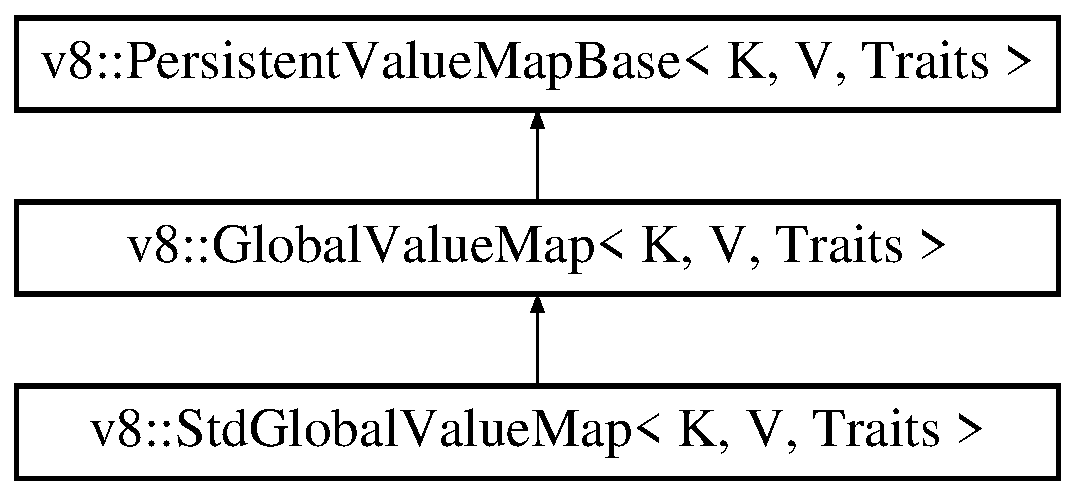
\includegraphics[height=3.000000cm]{classv8_1_1StdGlobalValueMap}
\end{center}
\end{figure}
\subsection*{Public Member Functions}
\begin{DoxyCompactItemize}
\item 
\hypertarget{classv8_1_1StdGlobalValueMap_af1025915a269b8b37af93ffc2ad5c3b1}{}{\bfseries Std\+Global\+Value\+Map} (\hyperlink{classv8_1_1Isolate}{Isolate} $\ast$isolate)\label{classv8_1_1StdGlobalValueMap_af1025915a269b8b37af93ffc2ad5c3b1}

\end{DoxyCompactItemize}
\subsection*{Additional Inherited Members}


\subsection{Detailed Description}
\subsubsection*{template$<$typename K, typename V, typename Traits = Default\+Global\+Map\+Traits$<$\+K, V$>$$>$class v8\+::\+Std\+Global\+Value\+Map$<$ K, V, Traits $>$}

A map that uses \hyperlink{classv8_1_1Global}{Global} as value and std\+::map as the backing implementation. Globals are held non-\/weak.

C++11 embedders don\textquotesingle{}t need this class, as they can use \hyperlink{classv8_1_1Global}{Global} directly in std containers. 

The documentation for this class was generated from the following file\+:\begin{DoxyCompactItemize}
\item 
v8/include/v8-\/util.\+h\end{DoxyCompactItemize}

\hypertarget{classv8_1_1StdMapTraits}{}\section{v8\+:\+:Std\+Map\+Traits$<$ K, V $>$ Class Template Reference}
\label{classv8_1_1StdMapTraits}\index{v8\+::\+Std\+Map\+Traits$<$ K, V $>$@{v8\+::\+Std\+Map\+Traits$<$ K, V $>$}}


{\ttfamily \#include $<$v8-\/util.\+h$>$}

Inheritance diagram for v8\+:\+:Std\+Map\+Traits$<$ K, V $>$\+:\begin{figure}[H]
\begin{center}
\leavevmode
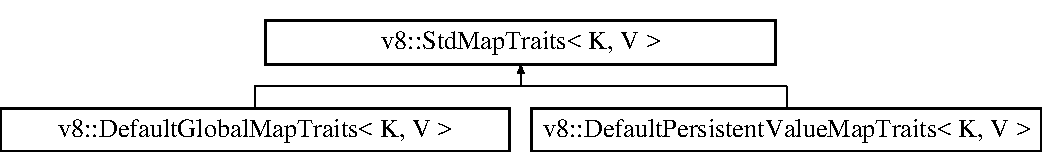
\includegraphics[height=2.000000cm]{classv8_1_1StdMapTraits}
\end{center}
\end{figure}
\subsection*{Public Types}
\begin{DoxyCompactItemize}
\item 
\mbox{\Hypertarget{classv8_1_1StdMapTraits_ac64cb78b3ef5cfbc35cf03837552e4ea}\label{classv8_1_1StdMapTraits_ac64cb78b3ef5cfbc35cf03837552e4ea}} 
typedef std\+::map$<$ K, \mbox{\hyperlink{classuintptr__t}{Persistent\+Container\+Value}} $>$ {\bfseries Impl}
\item 
\mbox{\Hypertarget{classv8_1_1StdMapTraits_ad20ef2022e83bfba6dcee23a2a34098e}\label{classv8_1_1StdMapTraits_ad20ef2022e83bfba6dcee23a2a34098e}} 
typedef Impl\+::iterator {\bfseries Iterator}
\end{DoxyCompactItemize}
\subsection*{Static Public Member Functions}
\begin{DoxyCompactItemize}
\item 
\mbox{\Hypertarget{classv8_1_1StdMapTraits_a63765723a9d6457ef47a42f79b13eaf7}\label{classv8_1_1StdMapTraits_a63765723a9d6457ef47a42f79b13eaf7}} 
static \mbox{\hyperlink{classbool}{bool}} {\bfseries Empty} (Impl $\ast$impl)
\item 
\mbox{\Hypertarget{classv8_1_1StdMapTraits_a60bd7720bbc6e662d948cf05283a009d}\label{classv8_1_1StdMapTraits_a60bd7720bbc6e662d948cf05283a009d}} 
static \mbox{\hyperlink{classsize__t}{size\+\_\+t}} {\bfseries Size} (Impl $\ast$impl)
\item 
\mbox{\Hypertarget{classv8_1_1StdMapTraits_ae018f70b3284ffda2566c36156db8baa}\label{classv8_1_1StdMapTraits_ae018f70b3284ffda2566c36156db8baa}} 
static void {\bfseries Swap} (Impl \&a, Impl \&b)
\item 
\mbox{\Hypertarget{classv8_1_1StdMapTraits_abc24bdbd2e7b054a7bd905759fad7987}\label{classv8_1_1StdMapTraits_abc24bdbd2e7b054a7bd905759fad7987}} 
static Iterator {\bfseries Begin} (Impl $\ast$impl)
\item 
\mbox{\Hypertarget{classv8_1_1StdMapTraits_a3ac36ae9e3b5585faeb66bb744c24183}\label{classv8_1_1StdMapTraits_a3ac36ae9e3b5585faeb66bb744c24183}} 
static Iterator {\bfseries End} (Impl $\ast$impl)
\item 
\mbox{\Hypertarget{classv8_1_1StdMapTraits_aa90a541b794946054fbc1e76e3976c4f}\label{classv8_1_1StdMapTraits_aa90a541b794946054fbc1e76e3976c4f}} 
static K {\bfseries Key} (Iterator it)
\item 
\mbox{\Hypertarget{classv8_1_1StdMapTraits_ad85f9d7e2ac639208fbce6b04d2436ad}\label{classv8_1_1StdMapTraits_ad85f9d7e2ac639208fbce6b04d2436ad}} 
static \mbox{\hyperlink{classuintptr__t}{Persistent\+Container\+Value}} {\bfseries Value} (Iterator it)
\item 
\mbox{\Hypertarget{classv8_1_1StdMapTraits_a2f41e206a3b1c9806253cca40d2891b1}\label{classv8_1_1StdMapTraits_a2f41e206a3b1c9806253cca40d2891b1}} 
static \mbox{\hyperlink{classuintptr__t}{Persistent\+Container\+Value}} {\bfseries Set} (Impl $\ast$impl, K key, \mbox{\hyperlink{classuintptr__t}{Persistent\+Container\+Value}} value)
\item 
\mbox{\Hypertarget{classv8_1_1StdMapTraits_a96c6fa384a4f7b7a64b464457ff347c2}\label{classv8_1_1StdMapTraits_a96c6fa384a4f7b7a64b464457ff347c2}} 
static \mbox{\hyperlink{classuintptr__t}{Persistent\+Container\+Value}} {\bfseries Get} (Impl $\ast$impl, K key)
\item 
\mbox{\Hypertarget{classv8_1_1StdMapTraits_ad35e42652392e70dd23fa4b69b9800ea}\label{classv8_1_1StdMapTraits_ad35e42652392e70dd23fa4b69b9800ea}} 
static \mbox{\hyperlink{classuintptr__t}{Persistent\+Container\+Value}} {\bfseries Remove} (Impl $\ast$impl, K key)
\end{DoxyCompactItemize}


\subsection{Detailed Description}
\subsubsection*{template$<$typename K, typename V$>$\newline
class v8\+::\+Std\+Map\+Traits$<$ K, V $>$}

A default trait implementation for \mbox{\hyperlink{classv8_1_1PersistentValueMap}{Persistent\+Value\+Map}} which uses std\+::map as a backing map.

Users will have to implement their own weak callbacks \& dispose traits. 

Definition at line 38 of file v8-\/util.\+h.



The documentation for this class was generated from the following file\+:\begin{DoxyCompactItemize}
\item 
v8/include/v8-\/util.\+h\end{DoxyCompactItemize}

\hypertarget{classv8_1_1StdPersistentValueMap}{}\section{v8\+:\+:Std\+Persistent\+Value\+Map$<$ K, V, Traits $>$ Class Template Reference}
\label{classv8_1_1StdPersistentValueMap}\index{v8\+::\+Std\+Persistent\+Value\+Map$<$ K, V, Traits $>$@{v8\+::\+Std\+Persistent\+Value\+Map$<$ K, V, Traits $>$}}


{\ttfamily \#include $<$v8-\/util.\+h$>$}

Inheritance diagram for v8\+:\+:Std\+Persistent\+Value\+Map$<$ K, V, Traits $>$\+:\begin{figure}[H]
\begin{center}
\leavevmode
\includegraphics[height=3.000000cm]{classv8_1_1StdPersistentValueMap}
\end{center}
\end{figure}
\subsection*{Public Member Functions}
\begin{DoxyCompactItemize}
\item 
\mbox{\Hypertarget{classv8_1_1StdPersistentValueMap_a44d7222a863267780db07c882056f73b}\label{classv8_1_1StdPersistentValueMap_a44d7222a863267780db07c882056f73b}} 
{\bfseries Std\+Persistent\+Value\+Map} (Isolate $\ast$isolate)
\end{DoxyCompactItemize}
\subsection*{Additional Inherited Members}


\subsection{Detailed Description}
\subsubsection*{template$<$typename K, typename V, typename Traits = Default\+Persistent\+Value\+Map\+Traits$<$\+K, V$>$$>$\newline
class v8\+::\+Std\+Persistent\+Value\+Map$<$ K, V, Traits $>$}

A map that uses \mbox{\hyperlink{classv8_1_1Global}{Global}} as value and std\+::map as the backing implementation. Persistents are held non-\/weak.

C++11 embedders don\textquotesingle{}t need this class, as they can use \mbox{\hyperlink{classv8_1_1Global}{Global}} directly in std containers. 

Definition at line 508 of file v8-\/util.\+h.



The documentation for this class was generated from the following file\+:\begin{DoxyCompactItemize}
\item 
v8/include/v8-\/util.\+h\end{DoxyCompactItemize}

\hypertarget{classv8_1_1ScriptCompiler_1_1StreamedSource}{}\section{v8\+:\+:Script\+Compiler\+:\+:Streamed\+Source Class Reference}
\label{classv8_1_1ScriptCompiler_1_1StreamedSource}\index{v8\+::\+Script\+Compiler\+::\+Streamed\+Source@{v8\+::\+Script\+Compiler\+::\+Streamed\+Source}}


{\ttfamily \#include $<$v8.\+h$>$}

\subsection*{Public Types}
\begin{DoxyCompactItemize}
\item 
enum {\bfseries Encoding} \{ {\bfseries O\+N\+E\+\_\+\+B\+Y\+TE}, 
{\bfseries T\+W\+O\+\_\+\+B\+Y\+TE}, 
{\bfseries U\+T\+F8}
 \}\hypertarget{classv8_1_1ScriptCompiler_1_1StreamedSource_a17b52f85ac22120e687b16357d662da2}{}\label{classv8_1_1ScriptCompiler_1_1StreamedSource_a17b52f85ac22120e687b16357d662da2}

\end{DoxyCompactItemize}
\subsection*{Public Member Functions}
\begin{DoxyCompactItemize}
\item 
{\bfseries Streamed\+Source} (\hyperlink{classv8_1_1ScriptCompiler_1_1ExternalSourceStream}{External\+Source\+Stream} $\ast$source\+\_\+stream, Encoding encoding)\hypertarget{classv8_1_1ScriptCompiler_1_1StreamedSource_a4da404a49e48a12927c743797833d8aa}{}\label{classv8_1_1ScriptCompiler_1_1StreamedSource_a4da404a49e48a12927c743797833d8aa}

\item 
const \hyperlink{structv8_1_1ScriptCompiler_1_1CachedData}{Cached\+Data} $\ast$ {\bfseries Get\+Cached\+Data} () const \hypertarget{classv8_1_1ScriptCompiler_1_1StreamedSource_a845dc408f6e2f98e51d6525836982873}{}\label{classv8_1_1ScriptCompiler_1_1StreamedSource_a845dc408f6e2f98e51d6525836982873}

\item 
internal\+::\+Streamed\+Source $\ast$ {\bfseries impl} () const \hypertarget{classv8_1_1ScriptCompiler_1_1StreamedSource_a60c3aa01ea04a6cd1aa1b7a5edb74c2b}{}\label{classv8_1_1ScriptCompiler_1_1StreamedSource_a60c3aa01ea04a6cd1aa1b7a5edb74c2b}

\end{DoxyCompactItemize}


\subsection{Detailed Description}
\hyperlink{classv8_1_1ScriptCompiler_1_1Source}{Source} code which can be streamed into \hyperlink{classv8_1_1V8}{V8} in pieces. It will be parsed while streaming. It can be compiled after the streaming is complete. \hyperlink{classv8_1_1ScriptCompiler_1_1StreamedSource}{Streamed\+Source} must be kept alive while the streaming task is ran (see \hyperlink{classv8_1_1ScriptCompiler_1_1ScriptStreamingTask}{Script\+Streaming\+Task} below). 

The documentation for this class was generated from the following file\+:\begin{DoxyCompactItemize}
\item 
v8/include/v8.\+h\end{DoxyCompactItemize}

\hypertarget{classv8_1_1String}{}\section{v8\+:\+:String Class Reference}
\label{classv8_1_1String}\index{v8\+::\+String@{v8\+::\+String}}


{\ttfamily \#include $<$v8.\+h$>$}

Inheritance diagram for v8\+:\+:String\+:\begin{figure}[H]
\begin{center}
\leavevmode
\includegraphics[height=5.000000cm]{classv8_1_1String}
\end{center}
\end{figure}
\subsection*{Classes}
\begin{DoxyCompactItemize}
\item 
class \mbox{\hyperlink{classv8_1_1String_1_1ExternalOneByteStringResource}{External\+One\+Byte\+String\+Resource}}
\item 
class \mbox{\hyperlink{classv8_1_1String_1_1ExternalStringResource}{External\+String\+Resource}}
\item 
class \mbox{\hyperlink{classv8_1_1String_1_1ExternalStringResourceBase}{External\+String\+Resource\+Base}}
\item 
class \mbox{\hyperlink{classv8_1_1String_1_1Utf8Value}{Utf8\+Value}}
\item 
class \mbox{\hyperlink{classv8_1_1String_1_1Value}{Value}}
\end{DoxyCompactItemize}
\subsection*{Public Types}
\begin{DoxyCompactItemize}
\item 
\mbox{\Hypertarget{classv8_1_1String_a2f4a2e9516c246eef602b889ce049c49}\label{classv8_1_1String_a2f4a2e9516c246eef602b889ce049c49}} 
enum {\bfseries Encoding} \{ {\bfseries U\+N\+K\+N\+O\+W\+N\+\_\+\+E\+N\+C\+O\+D\+I\+NG} = 0x1, 
{\bfseries T\+W\+O\+\_\+\+B\+Y\+T\+E\+\_\+\+E\+N\+C\+O\+D\+I\+NG} = 0x0, 
{\bfseries O\+N\+E\+\_\+\+B\+Y\+T\+E\+\_\+\+E\+N\+C\+O\+D\+I\+NG} = 0x8
 \}
\item 
enum \mbox{\hyperlink{classv8_1_1String_a9ce7f1458ffd08f8eb2b9c8dc056e616}{Write\+Options}} \{ \newline
{\bfseries N\+O\+\_\+\+O\+P\+T\+I\+O\+NS} = 0, 
{\bfseries H\+I\+N\+T\+\_\+\+M\+A\+N\+Y\+\_\+\+W\+R\+I\+T\+E\+S\+\_\+\+E\+X\+P\+E\+C\+T\+ED} = 1, 
{\bfseries N\+O\+\_\+\+N\+U\+L\+L\+\_\+\+T\+E\+R\+M\+I\+N\+A\+T\+I\+ON} = 2, 
{\bfseries P\+R\+E\+S\+E\+R\+V\+E\+\_\+\+O\+N\+E\+\_\+\+B\+Y\+T\+E\+\_\+\+N\+U\+LL} = 4, 
\newline
{\bfseries R\+E\+P\+L\+A\+C\+E\+\_\+\+I\+N\+V\+A\+L\+I\+D\+\_\+\+U\+T\+F8} = 8
 \}
\item 
\mbox{\Hypertarget{classv8_1_1String_a37620fb9fdc9b72ec9eea2a2aafaddee}\label{classv8_1_1String_a37620fb9fdc9b72ec9eea2a2aafaddee}} 
enum {\bfseries New\+String\+Type} \{ {\bfseries k\+Normal\+String} = static\+\_\+cast$<$int$>$(v8\+:\+:New\+String\+Type\+:\+:k\+Normal), 
{\bfseries k\+Internalized\+String} = static\+\_\+cast$<$int$>$(v8\+:\+:New\+String\+Type\+:\+:k\+Internalized)
 \}
\end{DoxyCompactItemize}
\subsection*{Public Member Functions}
\begin{DoxyCompactItemize}
\item 
\mbox{\hyperlink{classint}{int}} \mbox{\hyperlink{classv8_1_1String_afaa18eae27056bb7058f09920a238f53}{Length}} () const
\item 
\mbox{\hyperlink{classint}{int}} \mbox{\hyperlink{classv8_1_1String_af99433ee51ed45337e5b4536bd28a834}{Utf8\+Length}} (Isolate $\ast$isolate) const
\item 
\mbox{\hyperlink{classbool}{bool}} \mbox{\hyperlink{classv8_1_1String_a8f14ab3aff52295d2d3245081a1b29eb}{Is\+One\+Byte}} () const
\item 
\mbox{\hyperlink{classbool}{bool}} \mbox{\hyperlink{classv8_1_1String_a29b9bc5f71fba74af478e806b9d6a1d6}{Contains\+Only\+One\+Byte}} () const
\item 
\mbox{\Hypertarget{classv8_1_1String_a7196c4beb54cdbeaa31b84724c71a2dc}\label{classv8_1_1String_a7196c4beb54cdbeaa31b84724c71a2dc}} 
\mbox{\hyperlink{classint}{int}} {\bfseries Write} (Isolate $\ast$isolate, uint16\+\_\+t $\ast$buffer, \mbox{\hyperlink{classint}{int}} start=0, \mbox{\hyperlink{classint}{int}} length=-\/1, \mbox{\hyperlink{classint}{int}} options=N\+O\+\_\+\+O\+P\+T\+I\+O\+NS) const
\item 
\mbox{\Hypertarget{classv8_1_1String_a63989b39945308d79484c1a3c4c52730}\label{classv8_1_1String_a63989b39945308d79484c1a3c4c52730}} 
\mbox{\hyperlink{classint}{int}} {\bfseries Write\+One\+Byte} (Isolate $\ast$isolate, uint8\+\_\+t $\ast$buffer, \mbox{\hyperlink{classint}{int}} start=0, \mbox{\hyperlink{classint}{int}} length=-\/1, \mbox{\hyperlink{classint}{int}} options=N\+O\+\_\+\+O\+P\+T\+I\+O\+NS) const
\item 
\mbox{\Hypertarget{classv8_1_1String_a7a15f155614bef1fdda4dfc1072dc846}\label{classv8_1_1String_a7a15f155614bef1fdda4dfc1072dc846}} 
\mbox{\hyperlink{classint}{int}} {\bfseries Write\+Utf8} (Isolate $\ast$isolate, \mbox{\hyperlink{classchar}{char}} $\ast$buffer, \mbox{\hyperlink{classint}{int}} length=-\/1, \mbox{\hyperlink{classint}{int}} $\ast$nchars\+\_\+ref=nullptr, \mbox{\hyperlink{classint}{int}} options=N\+O\+\_\+\+O\+P\+T\+I\+O\+NS) const
\item 
\mbox{\hyperlink{classbool}{bool}} \mbox{\hyperlink{classv8_1_1String_a1d24faa97c6168221ec362c395d41ce1}{Is\+External}} () const
\item 
\mbox{\hyperlink{classbool}{bool}} \mbox{\hyperlink{classv8_1_1String_a29b5d1786d906b84e10a5cab9451f976}{Is\+External\+One\+Byte}} () const
\item 
V8\+\_\+\+I\+N\+L\+I\+NE \mbox{\hyperlink{classv8_1_1String_1_1ExternalStringResourceBase}{External\+String\+Resource\+Base}} $\ast$ \mbox{\hyperlink{classv8_1_1String_a3031c6406f3f84bbc2d9810477a07489}{Get\+External\+String\+Resource\+Base}} (Encoding $\ast$encoding\+\_\+out) const
\item 
V8\+\_\+\+I\+N\+L\+I\+NE \mbox{\hyperlink{classv8_1_1String_1_1ExternalStringResource}{External\+String\+Resource}} $\ast$ \mbox{\hyperlink{classv8_1_1String_ac751c8c239eb213a879204cab6787883}{Get\+External\+String\+Resource}} () const
\item 
const \mbox{\hyperlink{classv8_1_1String_1_1ExternalOneByteStringResource}{External\+One\+Byte\+String\+Resource}} $\ast$ \mbox{\hyperlink{classv8_1_1String_af362afb9835e123ad28c5255964af793}{Get\+External\+One\+Byte\+String\+Resource}} () const
\item 
\mbox{\hyperlink{classbool}{bool}} \mbox{\hyperlink{classv8_1_1String_a5efd1eba40c1fa8a6aae2c4a175a63be}{Make\+External}} (\mbox{\hyperlink{classv8_1_1String_1_1ExternalStringResource}{External\+String\+Resource}} $\ast$resource)
\item 
\mbox{\hyperlink{classbool}{bool}} \mbox{\hyperlink{classv8_1_1String_a607d632c720eec5133649f522aefa944}{Make\+External}} (\mbox{\hyperlink{classv8_1_1String_1_1ExternalOneByteStringResource}{External\+One\+Byte\+String\+Resource}} $\ast$resource)
\item 
\mbox{\hyperlink{classbool}{bool}} \mbox{\hyperlink{classv8_1_1String_a0fe076838af046506ffebbfadcde812a}{Can\+Make\+External}} ()
\item 
\mbox{\hyperlink{classbool}{bool}} \mbox{\hyperlink{classv8_1_1String_aaca2109ba1c2c50e45d40d7b79edb01c}{String\+Equals}} (\mbox{\hyperlink{classv8_1_1Local}{Local}}$<$ \mbox{\hyperlink{classv8_1_1String}{String}} $>$ str)
\end{DoxyCompactItemize}
\subsection*{Static Public Member Functions}
\begin{DoxyCompactItemize}
\item 
static V8\+\_\+\+I\+N\+L\+I\+NE \mbox{\hyperlink{classv8_1_1Local}{Local}}$<$ \mbox{\hyperlink{classv8_1_1String}{String}} $>$ \mbox{\hyperlink{classv8_1_1String_aa393d47baa54467fe57001065e49194b}{Empty}} (Isolate $\ast$isolate)
\item 
\mbox{\Hypertarget{classv8_1_1String_a826d60798dc152cea64a7636737b03b9}\label{classv8_1_1String_a826d60798dc152cea64a7636737b03b9}} 
static V8\+\_\+\+I\+N\+L\+I\+NE \mbox{\hyperlink{classv8_1_1String}{String}} $\ast$ {\bfseries Cast} (\mbox{\hyperlink{classv8_1_1Value}{v8\+::\+Value}} $\ast$obj)
\item 
static \mbox{\hyperlink{classv8_1_1String_aa9d64688e3535b3daabafcc46a59ce5a}{V8\+\_\+\+D\+E\+P\+R\+E\+C\+A\+T\+E\+\_\+\+S\+O\+ON}} (\char`\"{}Use maybe version\char`\"{}, Local$<$ \mbox{\hyperlink{classv8_1_1String}{String}} $>$ \mbox{\hyperlink{classv8_1_1String_a745e88987f6d7e01cb82e12ab9fc8703}{New\+From\+Utf8}}(Isolate $\ast$isolate, const \mbox{\hyperlink{classchar}{char}} $\ast$data, New\+String\+Type \mbox{\hyperlink{classstd_1_1conditional_1_1type}{type}}=k\+Normal\+String, \mbox{\hyperlink{classint}{int}} length=-\/1))
\item 
static V8\+\_\+\+W\+A\+R\+N\+\_\+\+U\+N\+U\+S\+E\+D\+\_\+\+R\+E\+S\+U\+LT \mbox{\hyperlink{classv8_1_1MaybeLocal}{Maybe\+Local}}$<$ \mbox{\hyperlink{classv8_1_1String}{String}} $>$ \mbox{\hyperlink{classv8_1_1String_a745e88987f6d7e01cb82e12ab9fc8703}{New\+From\+Utf8}} (Isolate $\ast$isolate, const \mbox{\hyperlink{classchar}{char}} $\ast$data, \mbox{\hyperlink{namespacev8_ac9163ab12fb3b2a95907a3a0367c6095}{v8\+::\+New\+String\+Type}} \mbox{\hyperlink{classstd_1_1conditional_1_1type}{type}}, \mbox{\hyperlink{classint}{int}} length=-\/1)
\item 
static V8\+\_\+\+W\+A\+R\+N\+\_\+\+U\+N\+U\+S\+E\+D\+\_\+\+R\+E\+S\+U\+LT \mbox{\hyperlink{classv8_1_1MaybeLocal}{Maybe\+Local}}$<$ \mbox{\hyperlink{classv8_1_1String}{String}} $>$ \mbox{\hyperlink{classv8_1_1String_ac9e61b74b58ad14389882c5030843972}{New\+From\+One\+Byte}} (Isolate $\ast$isolate, const uint8\+\_\+t $\ast$data, \mbox{\hyperlink{namespacev8_ac9163ab12fb3b2a95907a3a0367c6095}{v8\+::\+New\+String\+Type}} \mbox{\hyperlink{classstd_1_1conditional_1_1type}{type}}, \mbox{\hyperlink{classint}{int}} length=-\/1)
\item 
static \mbox{\hyperlink{classv8_1_1String_aeab948105979e2ffd61eb552b0da4e50}{V8\+\_\+\+D\+E\+P\+R\+E\+C\+A\+T\+E\+\_\+\+S\+O\+ON}} (\char`\"{}Use maybe version\char`\"{}, Local$<$ \mbox{\hyperlink{classv8_1_1String}{String}} $>$ \mbox{\hyperlink{classv8_1_1String_a6b3efe5df1016e4f9f485e79b0acdf5b}{New\+From\+Two\+Byte}}(Isolate $\ast$isolate, const uint16\+\_\+t $\ast$data, New\+String\+Type \mbox{\hyperlink{classstd_1_1conditional_1_1type}{type}}=k\+Normal\+String, \mbox{\hyperlink{classint}{int}} length=-\/1))
\item 
static V8\+\_\+\+W\+A\+R\+N\+\_\+\+U\+N\+U\+S\+E\+D\+\_\+\+R\+E\+S\+U\+LT \mbox{\hyperlink{classv8_1_1MaybeLocal}{Maybe\+Local}}$<$ \mbox{\hyperlink{classv8_1_1String}{String}} $>$ \mbox{\hyperlink{classv8_1_1String_a6b3efe5df1016e4f9f485e79b0acdf5b}{New\+From\+Two\+Byte}} (Isolate $\ast$isolate, const uint16\+\_\+t $\ast$data, \mbox{\hyperlink{namespacev8_ac9163ab12fb3b2a95907a3a0367c6095}{v8\+::\+New\+String\+Type}} \mbox{\hyperlink{classstd_1_1conditional_1_1type}{type}}, \mbox{\hyperlink{classint}{int}} length=-\/1)
\item 
static \mbox{\hyperlink{classv8_1_1Local}{Local}}$<$ \mbox{\hyperlink{classv8_1_1String}{String}} $>$ \mbox{\hyperlink{classv8_1_1String_a7ca729608359a02c17631fcc8ae7b8d7}{Concat}} (Isolate $\ast$isolate, \mbox{\hyperlink{classv8_1_1Local}{Local}}$<$ \mbox{\hyperlink{classv8_1_1String}{String}} $>$ left, \mbox{\hyperlink{classv8_1_1Local}{Local}}$<$ \mbox{\hyperlink{classv8_1_1String}{String}} $>$ right)
\item 
static V8\+\_\+\+W\+A\+R\+N\+\_\+\+U\+N\+U\+S\+E\+D\+\_\+\+R\+E\+S\+U\+LT \mbox{\hyperlink{classv8_1_1MaybeLocal}{Maybe\+Local}}$<$ \mbox{\hyperlink{classv8_1_1String}{String}} $>$ \mbox{\hyperlink{classv8_1_1String_a31979e3688dfeab2f74b90a1bec50f9b}{New\+External\+Two\+Byte}} (Isolate $\ast$isolate, \mbox{\hyperlink{classv8_1_1String_1_1ExternalStringResource}{External\+String\+Resource}} $\ast$resource)
\item 
static \mbox{\hyperlink{classv8_1_1String_ad7186b5cfdddffbee8235a7216f31a67}{V8\+\_\+\+D\+E\+P\+R\+E\+C\+A\+T\+E\+\_\+\+S\+O\+ON}} (\char`\"{}Use maybe version\char`\"{}, Local$<$ \mbox{\hyperlink{classv8_1_1String}{String}} $>$ New\+External(Isolate $\ast$isolate, \mbox{\hyperlink{classv8_1_1String_1_1ExternalOneByteStringResource}{External\+One\+Byte\+String\+Resource}} $\ast$resource))
\item 
\mbox{\Hypertarget{classv8_1_1String_a7f104356e56751f0a0223e28786cd801}\label{classv8_1_1String_a7f104356e56751f0a0223e28786cd801}} 
static V8\+\_\+\+W\+A\+R\+N\+\_\+\+U\+N\+U\+S\+E\+D\+\_\+\+R\+E\+S\+U\+LT \mbox{\hyperlink{classv8_1_1MaybeLocal}{Maybe\+Local}}$<$ \mbox{\hyperlink{classv8_1_1String}{String}} $>$ {\bfseries New\+External\+One\+Byte} (Isolate $\ast$isolate, \mbox{\hyperlink{classv8_1_1String_1_1ExternalOneByteStringResource}{External\+One\+Byte\+String\+Resource}} $\ast$resource)
\end{DoxyCompactItemize}
\subsection*{Static Public Attributes}
\begin{DoxyCompactItemize}
\item 
static constexpr \mbox{\hyperlink{classint}{int}} {\bfseries k\+Max\+Length}
\end{DoxyCompactItemize}


\subsection{Detailed Description}
A Java\+Script string value (E\+C\+M\+A-\/262, 4.\+3.\+17). 

Definition at line 2537 of file v8.\+h.



\subsection{Member Enumeration Documentation}
\mbox{\Hypertarget{classv8_1_1String_a9ce7f1458ffd08f8eb2b9c8dc056e616}\label{classv8_1_1String_a9ce7f1458ffd08f8eb2b9c8dc056e616}} 
\index{v8\+::\+String@{v8\+::\+String}!Write\+Options@{Write\+Options}}
\index{Write\+Options@{Write\+Options}!v8\+::\+String@{v8\+::\+String}}
\subsubsection{\texorpdfstring{Write\+Options}{WriteOptions}}
{\footnotesize\ttfamily enum \mbox{\hyperlink{classv8_1_1String_a9ce7f1458ffd08f8eb2b9c8dc056e616}{v8\+::\+String\+::\+Write\+Options}}}

Write the contents of the string to an external buffer. If no arguments are given, expects the buffer to be large enough to hold the entire string and N\+U\+LL terminator. Copies the contents of the string and the N\+U\+LL terminator into the buffer.

Write\+Utf8 will not write partial U\+T\+F-\/8 sequences, preferring to stop before the end of the buffer.

Copies up to length characters into the output buffer. Only null-\/terminates if there is enough space in the buffer.


\begin{DoxyParams}{Parameters}
{\em buffer} & The buffer into which the string will be copied. \\
\hline
{\em start} & The starting position within the string at which copying begins. \\
\hline
{\em length} & The number of characters to copy from the string. For Write\+Utf8 the number of bytes in the buffer. \\
\hline
{\em nchars\+\_\+ref} & The number of characters written, can be N\+U\+LL. \\
\hline
{\em options} & Various options that might affect performance of this or subsequent operations. \\
\hline
\end{DoxyParams}
\begin{DoxyReturn}{Returns}
The number of characters copied to the buffer excluding the null terminator. For Write\+Utf8\+: The number of bytes copied to the buffer including the null terminator (if written). 
\end{DoxyReturn}


Definition at line 2599 of file v8.\+h.



\subsection{Member Function Documentation}
\mbox{\Hypertarget{classv8_1_1String_a0fe076838af046506ffebbfadcde812a}\label{classv8_1_1String_a0fe076838af046506ffebbfadcde812a}} 
\index{v8\+::\+String@{v8\+::\+String}!Can\+Make\+External@{Can\+Make\+External}}
\index{Can\+Make\+External@{Can\+Make\+External}!v8\+::\+String@{v8\+::\+String}}
\subsubsection{\texorpdfstring{Can\+Make\+External()}{CanMakeExternal()}}
{\footnotesize\ttfamily \mbox{\hyperlink{classbool}{bool}} v8\+::\+String\+::\+Can\+Make\+External (\begin{DoxyParamCaption}{ }\end{DoxyParamCaption})}

Returns true if this string can be made external. 

Definition at line 6678 of file api.\+cc.

\mbox{\Hypertarget{classv8_1_1String_a7ca729608359a02c17631fcc8ae7b8d7}\label{classv8_1_1String_a7ca729608359a02c17631fcc8ae7b8d7}} 
\index{v8\+::\+String@{v8\+::\+String}!Concat@{Concat}}
\index{Concat@{Concat}!v8\+::\+String@{v8\+::\+String}}
\subsubsection{\texorpdfstring{Concat()}{Concat()}}
{\footnotesize\ttfamily \mbox{\hyperlink{classv8_1_1Local}{Local}}$<$ \mbox{\hyperlink{classv8_1_1String}{String}} $>$ v8\+::\+String\+::\+Concat (\begin{DoxyParamCaption}\item[{Isolate $\ast$}]{isolate,  }\item[{\mbox{\hyperlink{classv8_1_1Local}{Local}}$<$ \mbox{\hyperlink{classv8_1_1String}{String}} $>$}]{left,  }\item[{\mbox{\hyperlink{classv8_1_1Local}{Local}}$<$ \mbox{\hyperlink{classv8_1_1String}{String}} $>$}]{right }\end{DoxyParamCaption})\hspace{0.3cm}{\ttfamily [static]}}

Creates a new string by concatenating the left and the right strings passed in as parameters. 

Definition at line 6552 of file api.\+cc.

\mbox{\Hypertarget{classv8_1_1String_a29b9bc5f71fba74af478e806b9d6a1d6}\label{classv8_1_1String_a29b9bc5f71fba74af478e806b9d6a1d6}} 
\index{v8\+::\+String@{v8\+::\+String}!Contains\+Only\+One\+Byte@{Contains\+Only\+One\+Byte}}
\index{Contains\+Only\+One\+Byte@{Contains\+Only\+One\+Byte}!v8\+::\+String@{v8\+::\+String}}
\subsubsection{\texorpdfstring{Contains\+Only\+One\+Byte()}{ContainsOnlyOneByte()}}
{\footnotesize\ttfamily \mbox{\hyperlink{classbool}{bool}} v8\+::\+String\+::\+Contains\+Only\+One\+Byte (\begin{DoxyParamCaption}{ }\end{DoxyParamCaption}) const}

Returns whether this string contain only one byte data, i.\+e. I\+S\+O-\/8859-\/1 code points. Will read the entire string in some cases. 

Definition at line 5294 of file api.\+cc.

\mbox{\Hypertarget{classv8_1_1String_aa393d47baa54467fe57001065e49194b}\label{classv8_1_1String_aa393d47baa54467fe57001065e49194b}} 
\index{v8\+::\+String@{v8\+::\+String}!Empty@{Empty}}
\index{Empty@{Empty}!v8\+::\+String@{v8\+::\+String}}
\subsubsection{\texorpdfstring{Empty()}{Empty()}}
{\footnotesize\ttfamily \mbox{\hyperlink{classv8_1_1Local}{Local}}$<$ \mbox{\hyperlink{classv8_1_1String}{String}} $>$ v8\+::\+String\+::\+Empty (\begin{DoxyParamCaption}\item[{Isolate $\ast$}]{isolate }\end{DoxyParamCaption})\hspace{0.3cm}{\ttfamily [static]}}

A zero length string. 

Definition at line 9913 of file v8.\+h.

\mbox{\Hypertarget{classv8_1_1String_af362afb9835e123ad28c5255964af793}\label{classv8_1_1String_af362afb9835e123ad28c5255964af793}} 
\index{v8\+::\+String@{v8\+::\+String}!Get\+External\+One\+Byte\+String\+Resource@{Get\+External\+One\+Byte\+String\+Resource}}
\index{Get\+External\+One\+Byte\+String\+Resource@{Get\+External\+One\+Byte\+String\+Resource}!v8\+::\+String@{v8\+::\+String}}
\subsubsection{\texorpdfstring{Get\+External\+One\+Byte\+String\+Resource()}{GetExternalOneByteStringResource()}}
{\footnotesize\ttfamily const \mbox{\hyperlink{classv8_1_1String_1_1ExternalOneByteStringResource}{v8\+::\+String\+::\+External\+One\+Byte\+String\+Resource}} $\ast$ v8\+::\+String\+::\+Get\+External\+One\+Byte\+String\+Resource (\begin{DoxyParamCaption}{ }\end{DoxyParamCaption}) const}

Get the \mbox{\hyperlink{classv8_1_1String_1_1ExternalOneByteStringResource}{External\+One\+Byte\+String\+Resource}} for an external one-\/byte string. Returns N\+U\+LL if \mbox{\hyperlink{classv8_1_1String_a29b5d1786d906b84e10a5cab9451f976}{Is\+External\+One\+Byte()}} doesn\textquotesingle{}t return true. 

Definition at line 5703 of file api.\+cc.

\mbox{\Hypertarget{classv8_1_1String_ac751c8c239eb213a879204cab6787883}\label{classv8_1_1String_ac751c8c239eb213a879204cab6787883}} 
\index{v8\+::\+String@{v8\+::\+String}!Get\+External\+String\+Resource@{Get\+External\+String\+Resource}}
\index{Get\+External\+String\+Resource@{Get\+External\+String\+Resource}!v8\+::\+String@{v8\+::\+String}}
\subsubsection{\texorpdfstring{Get\+External\+String\+Resource()}{GetExternalStringResource()}}
{\footnotesize\ttfamily \mbox{\hyperlink{classv8_1_1String_1_1ExternalStringResource}{String\+::\+External\+String\+Resource}} $\ast$ v8\+::\+String\+::\+Get\+External\+String\+Resource (\begin{DoxyParamCaption}{ }\end{DoxyParamCaption}) const}

Get the \mbox{\hyperlink{classv8_1_1String_1_1ExternalStringResource}{External\+String\+Resource}} for an external string. Returns N\+U\+LL if \mbox{\hyperlink{classv8_1_1String_a1d24faa97c6168221ec362c395d41ce1}{Is\+External()}} doesn\textquotesingle{}t return true. 

Definition at line 9922 of file v8.\+h.

\mbox{\Hypertarget{classv8_1_1String_a3031c6406f3f84bbc2d9810477a07489}\label{classv8_1_1String_a3031c6406f3f84bbc2d9810477a07489}} 
\index{v8\+::\+String@{v8\+::\+String}!Get\+External\+String\+Resource\+Base@{Get\+External\+String\+Resource\+Base}}
\index{Get\+External\+String\+Resource\+Base@{Get\+External\+String\+Resource\+Base}!v8\+::\+String@{v8\+::\+String}}
\subsubsection{\texorpdfstring{Get\+External\+String\+Resource\+Base()}{GetExternalStringResourceBase()}}
{\footnotesize\ttfamily \mbox{\hyperlink{classv8_1_1String_1_1ExternalStringResourceBase}{String\+::\+External\+String\+Resource\+Base}} $\ast$ v8\+::\+String\+::\+Get\+External\+String\+Resource\+Base (\begin{DoxyParamCaption}\item[{String\+::\+Encoding $\ast$}]{encoding\+\_\+out }\end{DoxyParamCaption}) const}

If the string is an external string, return the \mbox{\hyperlink{classv8_1_1String_1_1ExternalStringResourceBase}{External\+String\+Resource\+Base}} regardless of the encoding, otherwise return N\+U\+LL. The encoding of the string is returned in encoding\+\_\+out. 

Definition at line 9941 of file v8.\+h.

\mbox{\Hypertarget{classv8_1_1String_a1d24faa97c6168221ec362c395d41ce1}\label{classv8_1_1String_a1d24faa97c6168221ec362c395d41ce1}} 
\index{v8\+::\+String@{v8\+::\+String}!Is\+External@{Is\+External}}
\index{Is\+External@{Is\+External}!v8\+::\+String@{v8\+::\+String}}
\subsubsection{\texorpdfstring{Is\+External()}{IsExternal()}}
{\footnotesize\ttfamily \mbox{\hyperlink{classbool}{bool}} v8\+::\+String\+::\+Is\+External (\begin{DoxyParamCaption}{ }\end{DoxyParamCaption}) const}

Returns true if the string is external 

Definition at line 5605 of file api.\+cc.

\mbox{\Hypertarget{classv8_1_1String_a29b5d1786d906b84e10a5cab9451f976}\label{classv8_1_1String_a29b5d1786d906b84e10a5cab9451f976}} 
\index{v8\+::\+String@{v8\+::\+String}!Is\+External\+One\+Byte@{Is\+External\+One\+Byte}}
\index{Is\+External\+One\+Byte@{Is\+External\+One\+Byte}!v8\+::\+String@{v8\+::\+String}}
\subsubsection{\texorpdfstring{Is\+External\+One\+Byte()}{IsExternalOneByte()}}
{\footnotesize\ttfamily \mbox{\hyperlink{classbool}{bool}} v8\+::\+String\+::\+Is\+External\+One\+Byte (\begin{DoxyParamCaption}{ }\end{DoxyParamCaption}) const}

Returns true if the string is both external and one-\/byte. 

Definition at line 5611 of file api.\+cc.

\mbox{\Hypertarget{classv8_1_1String_a8f14ab3aff52295d2d3245081a1b29eb}\label{classv8_1_1String_a8f14ab3aff52295d2d3245081a1b29eb}} 
\index{v8\+::\+String@{v8\+::\+String}!Is\+One\+Byte@{Is\+One\+Byte}}
\index{Is\+One\+Byte@{Is\+One\+Byte}!v8\+::\+String@{v8\+::\+String}}
\subsubsection{\texorpdfstring{Is\+One\+Byte()}{IsOneByte()}}
{\footnotesize\ttfamily \mbox{\hyperlink{classbool}{bool}} v8\+::\+String\+::\+Is\+One\+Byte (\begin{DoxyParamCaption}{ }\end{DoxyParamCaption}) const}

Returns whether this string is known to contain only one byte data, i.\+e. I\+S\+O-\/8859-\/1 code points. Does not read the string. False negatives are possible. 

Definition at line 5181 of file api.\+cc.

\mbox{\Hypertarget{classv8_1_1String_afaa18eae27056bb7058f09920a238f53}\label{classv8_1_1String_afaa18eae27056bb7058f09920a238f53}} 
\index{v8\+::\+String@{v8\+::\+String}!Length@{Length}}
\index{Length@{Length}!v8\+::\+String@{v8\+::\+String}}
\subsubsection{\texorpdfstring{Length()}{Length()}}
{\footnotesize\ttfamily \mbox{\hyperlink{classint}{int}} v8\+::\+String\+::\+Length (\begin{DoxyParamCaption}{ }\end{DoxyParamCaption}) const}

Returns the number of characters (U\+T\+F-\/16 code units) in this string. 

Definition at line 5175 of file api.\+cc.

\mbox{\Hypertarget{classv8_1_1String_a5efd1eba40c1fa8a6aae2c4a175a63be}\label{classv8_1_1String_a5efd1eba40c1fa8a6aae2c4a175a63be}} 
\index{v8\+::\+String@{v8\+::\+String}!Make\+External@{Make\+External}}
\index{Make\+External@{Make\+External}!v8\+::\+String@{v8\+::\+String}}
\subsubsection{\texorpdfstring{Make\+External()}{MakeExternal()}\hspace{0.1cm}{\footnotesize\ttfamily [1/2]}}
{\footnotesize\ttfamily \mbox{\hyperlink{classbool}{bool}} v8\+::\+String\+::\+Make\+External (\begin{DoxyParamCaption}\item[{\mbox{\hyperlink{classv8_1_1String_1_1ExternalStringResource}{External\+String\+Resource}} $\ast$}]{resource }\end{DoxyParamCaption})}

Associate an external string resource with this string by transforming it in place so that existing references to this string in the Java\+Script heap will use the external string resource. The external string resource\textquotesingle{}s character contents need to be equivalent to this string. Returns true if the string has been changed to be an external string. The string is not modified if the operation fails. See New\+External for information on the lifetime of the resource. 

Definition at line 6621 of file api.\+cc.

\mbox{\Hypertarget{classv8_1_1String_a607d632c720eec5133649f522aefa944}\label{classv8_1_1String_a607d632c720eec5133649f522aefa944}} 
\index{v8\+::\+String@{v8\+::\+String}!Make\+External@{Make\+External}}
\index{Make\+External@{Make\+External}!v8\+::\+String@{v8\+::\+String}}
\subsubsection{\texorpdfstring{Make\+External()}{MakeExternal()}\hspace{0.1cm}{\footnotesize\ttfamily [2/2]}}
{\footnotesize\ttfamily \mbox{\hyperlink{classbool}{bool}} v8\+::\+String\+::\+Make\+External (\begin{DoxyParamCaption}\item[{\mbox{\hyperlink{classv8_1_1String_1_1ExternalOneByteStringResource}{External\+One\+Byte\+String\+Resource}} $\ast$}]{resource }\end{DoxyParamCaption})}

Associate an external string resource with this string by transforming it in place so that existing references to this string in the Java\+Script heap will use the external string resource. The external string resource\textquotesingle{}s character contents need to be equivalent to this string. Returns true if the string has been changed to be an external string. The string is not modified if the operation fails. See New\+External for information on the lifetime of the resource. 

Definition at line 6649 of file api.\+cc.

\mbox{\Hypertarget{classv8_1_1String_a31979e3688dfeab2f74b90a1bec50f9b}\label{classv8_1_1String_a31979e3688dfeab2f74b90a1bec50f9b}} 
\index{v8\+::\+String@{v8\+::\+String}!New\+External\+Two\+Byte@{New\+External\+Two\+Byte}}
\index{New\+External\+Two\+Byte@{New\+External\+Two\+Byte}!v8\+::\+String@{v8\+::\+String}}
\subsubsection{\texorpdfstring{New\+External\+Two\+Byte()}{NewExternalTwoByte()}}
{\footnotesize\ttfamily \mbox{\hyperlink{classv8_1_1MaybeLocal}{Maybe\+Local}}$<$ \mbox{\hyperlink{classv8_1_1String}{String}} $>$ v8\+::\+String\+::\+New\+External\+Two\+Byte (\begin{DoxyParamCaption}\item[{Isolate $\ast$}]{isolate,  }\item[{\mbox{\hyperlink{classv8_1_1String_1_1ExternalStringResource}{External\+String\+Resource}} $\ast$}]{resource }\end{DoxyParamCaption})\hspace{0.3cm}{\ttfamily [static]}}

Creates a new external string using the data defined in the given resource. When the external string is no longer live on V8\textquotesingle{}s heap the resource will be disposed by calling its Dispose method. The caller of this function should not otherwise delete or modify the resource. Neither should the underlying buffer be deallocated or modified except through the destructor of the external string resource. 

Definition at line 6569 of file api.\+cc.

\mbox{\Hypertarget{classv8_1_1String_ac9e61b74b58ad14389882c5030843972}\label{classv8_1_1String_ac9e61b74b58ad14389882c5030843972}} 
\index{v8\+::\+String@{v8\+::\+String}!New\+From\+One\+Byte@{New\+From\+One\+Byte}}
\index{New\+From\+One\+Byte@{New\+From\+One\+Byte}!v8\+::\+String@{v8\+::\+String}}
\subsubsection{\texorpdfstring{New\+From\+One\+Byte()}{NewFromOneByte()}}
{\footnotesize\ttfamily \mbox{\hyperlink{classv8_1_1MaybeLocal}{Maybe\+Local}}$<$ \mbox{\hyperlink{classv8_1_1String}{String}} $>$ v8\+::\+String\+::\+New\+From\+One\+Byte (\begin{DoxyParamCaption}\item[{Isolate $\ast$}]{isolate,  }\item[{const uint8\+\_\+t $\ast$}]{data,  }\item[{\mbox{\hyperlink{namespacev8_ac9163ab12fb3b2a95907a3a0367c6095}{v8\+::\+New\+String\+Type}}}]{type,  }\item[{\mbox{\hyperlink{classint}{int}}}]{length = {\ttfamily -\/1} }\end{DoxyParamCaption})\hspace{0.3cm}{\ttfamily [static]}}

Allocates a new string from Latin-\/1 data. Only returns an empty value when length $>$ k\+Max\+Length. 

Definition at line 6528 of file api.\+cc.

\mbox{\Hypertarget{classv8_1_1String_a6b3efe5df1016e4f9f485e79b0acdf5b}\label{classv8_1_1String_a6b3efe5df1016e4f9f485e79b0acdf5b}} 
\index{v8\+::\+String@{v8\+::\+String}!New\+From\+Two\+Byte@{New\+From\+Two\+Byte}}
\index{New\+From\+Two\+Byte@{New\+From\+Two\+Byte}!v8\+::\+String@{v8\+::\+String}}
\subsubsection{\texorpdfstring{New\+From\+Two\+Byte()}{NewFromTwoByte()}}
{\footnotesize\ttfamily \mbox{\hyperlink{classv8_1_1MaybeLocal}{Maybe\+Local}}$<$ \mbox{\hyperlink{classv8_1_1String}{String}} $>$ v8\+::\+String\+::\+New\+From\+Two\+Byte (\begin{DoxyParamCaption}\item[{Isolate $\ast$}]{isolate,  }\item[{const uint16\+\_\+t $\ast$}]{data,  }\item[{\mbox{\hyperlink{namespacev8_ac9163ab12fb3b2a95907a3a0367c6095}{v8\+::\+New\+String\+Type}}}]{type,  }\item[{\mbox{\hyperlink{classint}{int}}}]{length = {\ttfamily -\/1} }\end{DoxyParamCaption})\hspace{0.3cm}{\ttfamily [static]}}

Allocates a new string from U\+T\+F-\/16 data. Only returns an empty value when length $>$ k\+Max\+Length. 

Definition at line 6535 of file api.\+cc.

\mbox{\Hypertarget{classv8_1_1String_a745e88987f6d7e01cb82e12ab9fc8703}\label{classv8_1_1String_a745e88987f6d7e01cb82e12ab9fc8703}} 
\index{v8\+::\+String@{v8\+::\+String}!New\+From\+Utf8@{New\+From\+Utf8}}
\index{New\+From\+Utf8@{New\+From\+Utf8}!v8\+::\+String@{v8\+::\+String}}
\subsubsection{\texorpdfstring{New\+From\+Utf8()}{NewFromUtf8()}}
{\footnotesize\ttfamily \mbox{\hyperlink{classv8_1_1MaybeLocal}{Maybe\+Local}}$<$ \mbox{\hyperlink{classv8_1_1String}{String}} $>$ v8\+::\+String\+::\+New\+From\+Utf8 (\begin{DoxyParamCaption}\item[{Isolate $\ast$}]{isolate,  }\item[{const \mbox{\hyperlink{classchar}{char}} $\ast$}]{data,  }\item[{\mbox{\hyperlink{namespacev8_ac9163ab12fb3b2a95907a3a0367c6095}{v8\+::\+New\+String\+Type}}}]{type,  }\item[{\mbox{\hyperlink{classint}{int}}}]{length = {\ttfamily -\/1} }\end{DoxyParamCaption})\hspace{0.3cm}{\ttfamily [static]}}

Allocates a new string from U\+T\+F-\/8 data. Only returns an empty value when length $>$ k\+Max\+Length. 

Definition at line 6511 of file api.\+cc.

\mbox{\Hypertarget{classv8_1_1String_aaca2109ba1c2c50e45d40d7b79edb01c}\label{classv8_1_1String_aaca2109ba1c2c50e45d40d7b79edb01c}} 
\index{v8\+::\+String@{v8\+::\+String}!String\+Equals@{String\+Equals}}
\index{String\+Equals@{String\+Equals}!v8\+::\+String@{v8\+::\+String}}
\subsubsection{\texorpdfstring{String\+Equals()}{StringEquals()}}
{\footnotesize\ttfamily \mbox{\hyperlink{classbool}{bool}} v8\+::\+String\+::\+String\+Equals (\begin{DoxyParamCaption}\item[{\mbox{\hyperlink{classv8_1_1Local}{Local}}$<$ \mbox{\hyperlink{classv8_1_1String}{String}} $>$}]{str }\end{DoxyParamCaption})}

Returns true if the strings values are equal. Same as JS ==/===. 

Definition at line 6694 of file api.\+cc.

\mbox{\Hypertarget{classv8_1_1String_af99433ee51ed45337e5b4536bd28a834}\label{classv8_1_1String_af99433ee51ed45337e5b4536bd28a834}} 
\index{v8\+::\+String@{v8\+::\+String}!Utf8\+Length@{Utf8\+Length}}
\index{Utf8\+Length@{Utf8\+Length}!v8\+::\+String@{v8\+::\+String}}
\subsubsection{\texorpdfstring{Utf8\+Length()}{Utf8Length()}}
{\footnotesize\ttfamily \mbox{\hyperlink{classint}{int}} v8\+::\+String\+::\+Utf8\+Length (\begin{DoxyParamCaption}\item[{Isolate $\ast$}]{isolate }\end{DoxyParamCaption}) const}

Returns the number of bytes in the U\+T\+F-\/8 encoded representation of this string. 

Definition at line 5301 of file api.\+cc.

\mbox{\Hypertarget{classv8_1_1String_aa9d64688e3535b3daabafcc46a59ce5a}\label{classv8_1_1String_aa9d64688e3535b3daabafcc46a59ce5a}} 
\index{v8\+::\+String@{v8\+::\+String}!V8\+\_\+\+D\+E\+P\+R\+E\+C\+A\+T\+E\+\_\+\+S\+O\+ON@{V8\+\_\+\+D\+E\+P\+R\+E\+C\+A\+T\+E\+\_\+\+S\+O\+ON}}
\index{V8\+\_\+\+D\+E\+P\+R\+E\+C\+A\+T\+E\+\_\+\+S\+O\+ON@{V8\+\_\+\+D\+E\+P\+R\+E\+C\+A\+T\+E\+\_\+\+S\+O\+ON}!v8\+::\+String@{v8\+::\+String}}
\subsubsection{\texorpdfstring{V8\+\_\+\+D\+E\+P\+R\+E\+C\+A\+T\+E\+\_\+\+S\+O\+O\+N()}{V8\_DEPRECATE\_SOON()}\hspace{0.1cm}{\footnotesize\ttfamily [1/3]}}
{\footnotesize\ttfamily static v8\+::\+String\+::\+V8\+\_\+\+D\+E\+P\+R\+E\+C\+A\+T\+E\+\_\+\+S\+O\+ON (\begin{DoxyParamCaption}\item[{\char`\"{}Use maybe version\char`\"{}}]{,  }\item[{\mbox{\hyperlink{classv8_1_1Local}{Local}}$<$ \mbox{\hyperlink{classv8_1_1String}{String}} $>$ }]{New\+From\+Utf8Isolate $\ast$isolate, const char $\ast$data, New\+String\+Type type=k\+Normal\+String, int length=-\/1 }\end{DoxyParamCaption})\hspace{0.3cm}{\ttfamily [static]}}

Allocates a new string from U\+T\+F-\/8 data. \mbox{\Hypertarget{classv8_1_1String_aeab948105979e2ffd61eb552b0da4e50}\label{classv8_1_1String_aeab948105979e2ffd61eb552b0da4e50}} 
\index{v8\+::\+String@{v8\+::\+String}!V8\+\_\+\+D\+E\+P\+R\+E\+C\+A\+T\+E\+\_\+\+S\+O\+ON@{V8\+\_\+\+D\+E\+P\+R\+E\+C\+A\+T\+E\+\_\+\+S\+O\+ON}}
\index{V8\+\_\+\+D\+E\+P\+R\+E\+C\+A\+T\+E\+\_\+\+S\+O\+ON@{V8\+\_\+\+D\+E\+P\+R\+E\+C\+A\+T\+E\+\_\+\+S\+O\+ON}!v8\+::\+String@{v8\+::\+String}}
\subsubsection{\texorpdfstring{V8\+\_\+\+D\+E\+P\+R\+E\+C\+A\+T\+E\+\_\+\+S\+O\+O\+N()}{V8\_DEPRECATE\_SOON()}\hspace{0.1cm}{\footnotesize\ttfamily [2/3]}}
{\footnotesize\ttfamily static v8\+::\+String\+::\+V8\+\_\+\+D\+E\+P\+R\+E\+C\+A\+T\+E\+\_\+\+S\+O\+ON (\begin{DoxyParamCaption}\item[{\char`\"{}Use maybe version\char`\"{}}]{,  }\item[{\mbox{\hyperlink{classv8_1_1Local}{Local}}$<$ \mbox{\hyperlink{classv8_1_1String}{String}} $>$ }]{New\+From\+Two\+ByteIsolate $\ast$isolate, const uint16\+\_\+t $\ast$data, New\+String\+Type type=k\+Normal\+String, int length=-\/1 }\end{DoxyParamCaption})\hspace{0.3cm}{\ttfamily [static]}}

Allocates a new string from U\+T\+F-\/16 data. \mbox{\Hypertarget{classv8_1_1String_ad7186b5cfdddffbee8235a7216f31a67}\label{classv8_1_1String_ad7186b5cfdddffbee8235a7216f31a67}} 
\index{v8\+::\+String@{v8\+::\+String}!V8\+\_\+\+D\+E\+P\+R\+E\+C\+A\+T\+E\+\_\+\+S\+O\+ON@{V8\+\_\+\+D\+E\+P\+R\+E\+C\+A\+T\+E\+\_\+\+S\+O\+ON}}
\index{V8\+\_\+\+D\+E\+P\+R\+E\+C\+A\+T\+E\+\_\+\+S\+O\+ON@{V8\+\_\+\+D\+E\+P\+R\+E\+C\+A\+T\+E\+\_\+\+S\+O\+ON}!v8\+::\+String@{v8\+::\+String}}
\subsubsection{\texorpdfstring{V8\+\_\+\+D\+E\+P\+R\+E\+C\+A\+T\+E\+\_\+\+S\+O\+O\+N()}{V8\_DEPRECATE\_SOON()}\hspace{0.1cm}{\footnotesize\ttfamily [3/3]}}
{\footnotesize\ttfamily static v8\+::\+String\+::\+V8\+\_\+\+D\+E\+P\+R\+E\+C\+A\+T\+E\+\_\+\+S\+O\+ON (\begin{DoxyParamCaption}\item[{\char`\"{}Use maybe version\char`\"{}}]{,  }\item[{\mbox{\hyperlink{classv8_1_1Local}{Local}}$<$ \mbox{\hyperlink{classv8_1_1String}{String}} $>$ }]{New\+ExternalIsolate $\ast$isolate, External\+One\+Byte\+String\+Resource $\ast$resource }\end{DoxyParamCaption})\hspace{0.3cm}{\ttfamily [static]}}

Creates a new external string using the one-\/byte data defined in the given resource. When the external string is no longer live on V8\textquotesingle{}s heap the resource will be disposed by calling its Dispose method. The caller of this function should not otherwise delete or modify the resource. Neither should the underlying buffer be deallocated or modified except through the destructor of the external string resource. 

\subsection{Member Data Documentation}
\mbox{\Hypertarget{classv8_1_1String_a66259940a4836974906729017ff25fd2}\label{classv8_1_1String_a66259940a4836974906729017ff25fd2}} 
\index{v8\+::\+String@{v8\+::\+String}!k\+Max\+Length@{k\+Max\+Length}}
\index{k\+Max\+Length@{k\+Max\+Length}!v8\+::\+String@{v8\+::\+String}}
\subsubsection{\texorpdfstring{k\+Max\+Length}{kMaxLength}}
{\footnotesize\ttfamily constexpr \mbox{\hyperlink{classint}{int}} v8\+::\+String\+::k\+Max\+Length\hspace{0.3cm}{\ttfamily [static]}}

{\bfseries Initial value\+:}
\begin{DoxyCode}
= internal::kApiTaggedSize == 4
                                        ? (1 << 28) - 16
                                        : internal::kSmiMaxValue / 2 - 24
\end{DoxyCode}


Definition at line 2539 of file v8.\+h.



The documentation for this class was generated from the following files\+:\begin{DoxyCompactItemize}
\item 
v8/include/v8.\+h\item 
v8/src/api.\+cc\end{DoxyCompactItemize}

\hypertarget{classv8_1_1StringObject}{}\section{v8\+:\+:String\+Object Class Reference}
\label{classv8_1_1StringObject}\index{v8\+::\+String\+Object@{v8\+::\+String\+Object}}


{\ttfamily \#include $<$v8.\+h$>$}

Inheritance diagram for v8\+:\+:String\+Object\+:\begin{figure}[H]
\begin{center}
\leavevmode
\includegraphics[height=4.000000cm]{classv8_1_1StringObject}
\end{center}
\end{figure}
\subsection*{Public Member Functions}
\begin{DoxyCompactItemize}
\item 
\mbox{\Hypertarget{classv8_1_1StringObject_a728454fbe6e41dc3af72de0f72ffe371}\label{classv8_1_1StringObject_a728454fbe6e41dc3af72de0f72ffe371}} 
\mbox{\hyperlink{classv8_1_1Local}{Local}}$<$ \mbox{\hyperlink{classv8_1_1String}{String}} $>$ {\bfseries Value\+Of} () const
\end{DoxyCompactItemize}
\subsection*{Static Public Member Functions}
\begin{DoxyCompactItemize}
\item 
\mbox{\Hypertarget{classv8_1_1StringObject_a850b39ef363a85cd409dc31cd8ae7cfd}\label{classv8_1_1StringObject_a850b39ef363a85cd409dc31cd8ae7cfd}} 
static \mbox{\hyperlink{classv8_1_1Local}{Local}}$<$ \mbox{\hyperlink{classv8_1_1Value}{Value}} $>$ {\bfseries New} (Isolate $\ast$isolate, \mbox{\hyperlink{classv8_1_1Local}{Local}}$<$ \mbox{\hyperlink{classv8_1_1String}{String}} $>$ value)
\item 
\mbox{\Hypertarget{classv8_1_1StringObject_af01249353a4a9032f7791a6e7a4ff094}\label{classv8_1_1StringObject_af01249353a4a9032f7791a6e7a4ff094}} 
static V8\+\_\+\+I\+N\+L\+I\+NE \mbox{\hyperlink{classv8_1_1StringObject}{String\+Object}} $\ast$ {\bfseries Cast} (\mbox{\hyperlink{classv8_1_1Value}{Value}} $\ast$obj)
\end{DoxyCompactItemize}


\subsection{Detailed Description}
A \mbox{\hyperlink{classv8_1_1String}{String}} object (E\+C\+M\+A-\/262, 4.\+3.\+18). 

The documentation for this class was generated from the following file\+:\begin{DoxyCompactItemize}
\item 
v8/include/v8.\+h\end{DoxyCompactItemize}

\hypertarget{classv8_1_1Isolate_1_1SuppressMicrotaskExecutionScope}{}\section{v8\+:\+:Isolate\+:\+:Suppress\+Microtask\+Execution\+Scope Class Reference}
\label{classv8_1_1Isolate_1_1SuppressMicrotaskExecutionScope}\index{v8\+::\+Isolate\+::\+Suppress\+Microtask\+Execution\+Scope@{v8\+::\+Isolate\+::\+Suppress\+Microtask\+Execution\+Scope}}


{\ttfamily \#include $<$v8.\+h$>$}

\subsection*{Public Member Functions}
\begin{DoxyCompactItemize}
\item 
\mbox{\Hypertarget{classv8_1_1Isolate_1_1SuppressMicrotaskExecutionScope_a846d7dd39f4cfad4dfc4c8c785e4a65e}\label{classv8_1_1Isolate_1_1SuppressMicrotaskExecutionScope_a846d7dd39f4cfad4dfc4c8c785e4a65e}} 
{\bfseries Suppress\+Microtask\+Execution\+Scope} (\mbox{\hyperlink{classv8_1_1Isolate}{Isolate}} $\ast$isolate)
\item 
\mbox{\Hypertarget{classv8_1_1Isolate_1_1SuppressMicrotaskExecutionScope_ae4d7f51ceab47cabf1f78f65224ca95d}\label{classv8_1_1Isolate_1_1SuppressMicrotaskExecutionScope_ae4d7f51ceab47cabf1f78f65224ca95d}} 
{\bfseries Suppress\+Microtask\+Execution\+Scope} (const \mbox{\hyperlink{classv8_1_1Isolate_1_1SuppressMicrotaskExecutionScope}{Suppress\+Microtask\+Execution\+Scope}} \&)=delete
\item 
\mbox{\Hypertarget{classv8_1_1Isolate_1_1SuppressMicrotaskExecutionScope_a48038b7c5037f6a329c27ccffef0e71c}\label{classv8_1_1Isolate_1_1SuppressMicrotaskExecutionScope_a48038b7c5037f6a329c27ccffef0e71c}} 
\mbox{\hyperlink{classv8_1_1Isolate_1_1SuppressMicrotaskExecutionScope}{Suppress\+Microtask\+Execution\+Scope}} \& {\bfseries operator=} (const \mbox{\hyperlink{classv8_1_1Isolate_1_1SuppressMicrotaskExecutionScope}{Suppress\+Microtask\+Execution\+Scope}} \&)=delete
\end{DoxyCompactItemize}


\subsection{Detailed Description}
Do not run microtasks while this scope is active, even if microtasks are automatically executed otherwise. 

The documentation for this class was generated from the following file\+:\begin{DoxyCompactItemize}
\item 
v8/include/v8.\+h\end{DoxyCompactItemize}

\hypertarget{classv8_1_1Symbol}{}\section{v8\+:\+:Symbol Class Reference}
\label{classv8_1_1Symbol}\index{v8\+::\+Symbol@{v8\+::\+Symbol}}


{\ttfamily \#include $<$v8.\+h$>$}

Inheritance diagram for v8\+:\+:Symbol\+:\begin{figure}[H]
\begin{center}
\leavevmode
\includegraphics[height=5.000000cm]{classv8_1_1Symbol}
\end{center}
\end{figure}
\subsection*{Public Member Functions}
\begin{DoxyCompactItemize}
\item 
\mbox{\hyperlink{classv8_1_1Local}{Local}}$<$ \mbox{\hyperlink{classv8_1_1Value}{Value}} $>$ \mbox{\hyperlink{classv8_1_1Symbol_a8b6346ed4f396a1286fc50a95d84b79c}{Name}} () const
\end{DoxyCompactItemize}
\subsection*{Static Public Member Functions}
\begin{DoxyCompactItemize}
\item 
static \mbox{\hyperlink{classv8_1_1Local}{Local}}$<$ \mbox{\hyperlink{classv8_1_1Symbol}{Symbol}} $>$ \mbox{\hyperlink{classv8_1_1Symbol_ac241ffee8282d3067f8ed0da7be2adb8}{New}} (Isolate $\ast$isolate, \mbox{\hyperlink{classv8_1_1Local}{Local}}$<$ \mbox{\hyperlink{classv8_1_1String}{String}} $>$ name=\mbox{\hyperlink{classv8_1_1Local}{Local}}$<$ \mbox{\hyperlink{classv8_1_1String}{String}} $>$())
\item 
static \mbox{\hyperlink{classv8_1_1Local}{Local}}$<$ \mbox{\hyperlink{classv8_1_1Symbol}{Symbol}} $>$ \mbox{\hyperlink{classv8_1_1Symbol_a4bde7380260d3c1cab6289a8029b34c4}{For}} (Isolate $\ast$isolate, \mbox{\hyperlink{classv8_1_1Local}{Local}}$<$ \mbox{\hyperlink{classv8_1_1String}{String}} $>$ name)
\item 
static \mbox{\hyperlink{classv8_1_1Local}{Local}}$<$ \mbox{\hyperlink{classv8_1_1Symbol}{Symbol}} $>$ \mbox{\hyperlink{classv8_1_1Symbol_af1c88cf1c86bf5254bd60013e04de941}{For\+Api}} (Isolate $\ast$isolate, \mbox{\hyperlink{classv8_1_1Local}{Local}}$<$ \mbox{\hyperlink{classv8_1_1String}{String}} $>$ name)
\item 
\mbox{\Hypertarget{classv8_1_1Symbol_a9ce03e853ed34c0192bef63d88d2f9c6}\label{classv8_1_1Symbol_a9ce03e853ed34c0192bef63d88d2f9c6}} 
static \mbox{\hyperlink{classv8_1_1Local}{Local}}$<$ \mbox{\hyperlink{classv8_1_1Symbol}{Symbol}} $>$ {\bfseries Get\+Async\+Iterator} (Isolate $\ast$isolate)
\item 
\mbox{\Hypertarget{classv8_1_1Symbol_ad23ee69f0680db333469272554b07a6e}\label{classv8_1_1Symbol_ad23ee69f0680db333469272554b07a6e}} 
static \mbox{\hyperlink{classv8_1_1Local}{Local}}$<$ \mbox{\hyperlink{classv8_1_1Symbol}{Symbol}} $>$ {\bfseries Get\+Has\+Instance} (Isolate $\ast$isolate)
\item 
\mbox{\Hypertarget{classv8_1_1Symbol_acf0d506838dbf518537c17a72571c0bf}\label{classv8_1_1Symbol_acf0d506838dbf518537c17a72571c0bf}} 
static \mbox{\hyperlink{classv8_1_1Local}{Local}}$<$ \mbox{\hyperlink{classv8_1_1Symbol}{Symbol}} $>$ {\bfseries Get\+Is\+Concat\+Spreadable} (Isolate $\ast$isolate)
\item 
\mbox{\Hypertarget{classv8_1_1Symbol_a35aa1aca7135c5bf9052d8d067d126b1}\label{classv8_1_1Symbol_a35aa1aca7135c5bf9052d8d067d126b1}} 
static \mbox{\hyperlink{classv8_1_1Local}{Local}}$<$ \mbox{\hyperlink{classv8_1_1Symbol}{Symbol}} $>$ {\bfseries Get\+Iterator} (Isolate $\ast$isolate)
\item 
\mbox{\Hypertarget{classv8_1_1Symbol_a2372eac85db34c2c3665db1d3fcc4dac}\label{classv8_1_1Symbol_a2372eac85db34c2c3665db1d3fcc4dac}} 
static \mbox{\hyperlink{classv8_1_1Local}{Local}}$<$ \mbox{\hyperlink{classv8_1_1Symbol}{Symbol}} $>$ {\bfseries Get\+Match} (Isolate $\ast$isolate)
\item 
\mbox{\Hypertarget{classv8_1_1Symbol_a2492651242adc378e88fd6fbdf574db5}\label{classv8_1_1Symbol_a2492651242adc378e88fd6fbdf574db5}} 
static \mbox{\hyperlink{classv8_1_1Local}{Local}}$<$ \mbox{\hyperlink{classv8_1_1Symbol}{Symbol}} $>$ {\bfseries Get\+Replace} (Isolate $\ast$isolate)
\item 
\mbox{\Hypertarget{classv8_1_1Symbol_a6b825709dea7625c6bc5dec9ce5c2d18}\label{classv8_1_1Symbol_a6b825709dea7625c6bc5dec9ce5c2d18}} 
static \mbox{\hyperlink{classv8_1_1Local}{Local}}$<$ \mbox{\hyperlink{classv8_1_1Symbol}{Symbol}} $>$ {\bfseries Get\+Search} (Isolate $\ast$isolate)
\item 
\mbox{\Hypertarget{classv8_1_1Symbol_a410b12cdc6f02830484367f579145cf0}\label{classv8_1_1Symbol_a410b12cdc6f02830484367f579145cf0}} 
static \mbox{\hyperlink{classv8_1_1Local}{Local}}$<$ \mbox{\hyperlink{classv8_1_1Symbol}{Symbol}} $>$ {\bfseries Get\+Split} (Isolate $\ast$isolate)
\item 
\mbox{\Hypertarget{classv8_1_1Symbol_ae038d3f766cbe82f994be4303264235a}\label{classv8_1_1Symbol_ae038d3f766cbe82f994be4303264235a}} 
static \mbox{\hyperlink{classv8_1_1Local}{Local}}$<$ \mbox{\hyperlink{classv8_1_1Symbol}{Symbol}} $>$ {\bfseries Get\+To\+Primitive} (Isolate $\ast$isolate)
\item 
\mbox{\Hypertarget{classv8_1_1Symbol_ab595ae7100ce23e4b1677ecab02f5972}\label{classv8_1_1Symbol_ab595ae7100ce23e4b1677ecab02f5972}} 
static \mbox{\hyperlink{classv8_1_1Local}{Local}}$<$ \mbox{\hyperlink{classv8_1_1Symbol}{Symbol}} $>$ {\bfseries Get\+To\+String\+Tag} (Isolate $\ast$isolate)
\item 
\mbox{\Hypertarget{classv8_1_1Symbol_acf5b5220a820f6ed1e61500292ebec13}\label{classv8_1_1Symbol_acf5b5220a820f6ed1e61500292ebec13}} 
static \mbox{\hyperlink{classv8_1_1Local}{Local}}$<$ \mbox{\hyperlink{classv8_1_1Symbol}{Symbol}} $>$ {\bfseries Get\+Unscopables} (Isolate $\ast$isolate)
\item 
\mbox{\Hypertarget{classv8_1_1Symbol_aab15294631d6e6eb95b2c8bd1e7eb861}\label{classv8_1_1Symbol_aab15294631d6e6eb95b2c8bd1e7eb861}} 
static V8\+\_\+\+I\+N\+L\+I\+NE \mbox{\hyperlink{classv8_1_1Symbol}{Symbol}} $\ast$ {\bfseries Cast} (\mbox{\hyperlink{classv8_1_1Value}{Value}} $\ast$obj)
\end{DoxyCompactItemize}


\subsection{Detailed Description}
A Java\+Script symbol (E\+C\+M\+A-\/262 edition 6) 

Definition at line 2931 of file v8.\+h.



\subsection{Member Function Documentation}
\mbox{\Hypertarget{classv8_1_1Symbol_a4bde7380260d3c1cab6289a8029b34c4}\label{classv8_1_1Symbol_a4bde7380260d3c1cab6289a8029b34c4}} 
\index{v8\+::\+Symbol@{v8\+::\+Symbol}!For@{For}}
\index{For@{For}!v8\+::\+Symbol@{v8\+::\+Symbol}}
\subsubsection{\texorpdfstring{For()}{For()}}
{\footnotesize\ttfamily \mbox{\hyperlink{classv8_1_1Local}{Local}}$<$ \mbox{\hyperlink{classv8_1_1Symbol}{Symbol}} $>$ v8\+::\+Symbol\+::\+For (\begin{DoxyParamCaption}\item[{Isolate $\ast$}]{isolate,  }\item[{\mbox{\hyperlink{classv8_1_1Local}{Local}}$<$ \mbox{\hyperlink{classv8_1_1String}{String}} $>$}]{name }\end{DoxyParamCaption})\hspace{0.3cm}{\ttfamily [static]}}

Access global symbol registry. Note that symbols created this way are never collected, so they should only be used for statically fixed properties. Also, there is only one global name space for the names used as keys. To minimize the potential for clashes, use qualified names as keys. 

Definition at line 7906 of file api.\+cc.

\mbox{\Hypertarget{classv8_1_1Symbol_af1c88cf1c86bf5254bd60013e04de941}\label{classv8_1_1Symbol_af1c88cf1c86bf5254bd60013e04de941}} 
\index{v8\+::\+Symbol@{v8\+::\+Symbol}!For\+Api@{For\+Api}}
\index{For\+Api@{For\+Api}!v8\+::\+Symbol@{v8\+::\+Symbol}}
\subsubsection{\texorpdfstring{For\+Api()}{ForApi()}}
{\footnotesize\ttfamily \mbox{\hyperlink{classv8_1_1Local}{Local}}$<$ \mbox{\hyperlink{classv8_1_1Symbol}{Symbol}} $>$ v8\+::\+Symbol\+::\+For\+Api (\begin{DoxyParamCaption}\item[{Isolate $\ast$}]{isolate,  }\item[{\mbox{\hyperlink{classv8_1_1Local}{Local}}$<$ \mbox{\hyperlink{classv8_1_1String}{String}} $>$}]{name }\end{DoxyParamCaption})\hspace{0.3cm}{\ttfamily [static]}}

Retrieve a global symbol. Similar to $\vert$\+For$\vert$, but using a separate registry that is not accessible by (and cannot clash with) Java\+Script code. 

Definition at line 7914 of file api.\+cc.

\mbox{\Hypertarget{classv8_1_1Symbol_a8b6346ed4f396a1286fc50a95d84b79c}\label{classv8_1_1Symbol_a8b6346ed4f396a1286fc50a95d84b79c}} 
\index{v8\+::\+Symbol@{v8\+::\+Symbol}!Name@{Name}}
\index{Name@{Name}!v8\+::\+Symbol@{v8\+::\+Symbol}}
\subsubsection{\texorpdfstring{Name()}{Name()}}
{\footnotesize\ttfamily \mbox{\hyperlink{classv8_1_1Local}{Local}}$<$ \mbox{\hyperlink{classv8_1_1Value}{Value}} $>$ v8\+::\+Symbol\+::\+Name (\begin{DoxyParamCaption}{ }\end{DoxyParamCaption}) const}

Returns the print name string of the symbol, or undefined if none. 

Definition at line 5718 of file api.\+cc.

\mbox{\Hypertarget{classv8_1_1Symbol_ac241ffee8282d3067f8ed0da7be2adb8}\label{classv8_1_1Symbol_ac241ffee8282d3067f8ed0da7be2adb8}} 
\index{v8\+::\+Symbol@{v8\+::\+Symbol}!New@{New}}
\index{New@{New}!v8\+::\+Symbol@{v8\+::\+Symbol}}
\subsubsection{\texorpdfstring{New()}{New()}}
{\footnotesize\ttfamily \mbox{\hyperlink{classv8_1_1Local}{Local}}$<$ \mbox{\hyperlink{classv8_1_1Symbol}{Symbol}} $>$ v8\+::\+Symbol\+::\+New (\begin{DoxyParamCaption}\item[{Isolate $\ast$}]{isolate,  }\item[{\mbox{\hyperlink{classv8_1_1Local}{Local}}$<$ \mbox{\hyperlink{classv8_1_1String}{String}} $>$}]{name = {\ttfamily \mbox{\hyperlink{classv8_1_1Local}{Local}}$<$\mbox{\hyperlink{classv8_1_1String}{String}}$>$()} }\end{DoxyParamCaption})\hspace{0.3cm}{\ttfamily [static]}}

Create a symbol. If name is not empty, it will be used as the description. 

Definition at line 7896 of file api.\+cc.



The documentation for this class was generated from the following files\+:\begin{DoxyCompactItemize}
\item 
v8/include/v8.\+h\item 
v8/src/api.\+cc\end{DoxyCompactItemize}

\hypertarget{classv8_1_1SymbolObject}{}\section{v8\+:\+:Symbol\+Object Class Reference}
\label{classv8_1_1SymbolObject}\index{v8\+::\+Symbol\+Object@{v8\+::\+Symbol\+Object}}


{\ttfamily \#include $<$v8.\+h$>$}

Inheritance diagram for v8\+:\+:Symbol\+Object\+:\begin{figure}[H]
\begin{center}
\leavevmode
\includegraphics[height=4.000000cm]{classv8_1_1SymbolObject}
\end{center}
\end{figure}
\subsection*{Public Member Functions}
\begin{DoxyCompactItemize}
\item 
\hypertarget{classv8_1_1SymbolObject_a4a3b439c6784a4a8d9bdc5a246e12b85}{}\hyperlink{classv8_1_1Local}{Local}$<$ \hyperlink{classv8_1_1Symbol}{Symbol} $>$ {\bfseries Value\+Of} () const \label{classv8_1_1SymbolObject_a4a3b439c6784a4a8d9bdc5a246e12b85}

\end{DoxyCompactItemize}
\subsection*{Static Public Member Functions}
\begin{DoxyCompactItemize}
\item 
\hypertarget{classv8_1_1SymbolObject_a3a3dc109d1207e4fe20671c17f5426c0}{}static \hyperlink{classv8_1_1Local}{Local}$<$ \hyperlink{classv8_1_1Value}{Value} $>$ {\bfseries New} (\hyperlink{classv8_1_1Isolate}{Isolate} $\ast$isolate, \hyperlink{classv8_1_1Local}{Local}$<$ \hyperlink{classv8_1_1Symbol}{Symbol} $>$ value)\label{classv8_1_1SymbolObject_a3a3dc109d1207e4fe20671c17f5426c0}

\item 
\hypertarget{classv8_1_1SymbolObject_aa98d7c4211bd55e347ee8169143fcec9}{}static V8\+\_\+\+I\+N\+L\+I\+N\+E \hyperlink{classv8_1_1SymbolObject}{Symbol\+Object} $\ast$ {\bfseries Cast} (\hyperlink{classv8_1_1Value}{v8\+::\+Value} $\ast$obj)\label{classv8_1_1SymbolObject_aa98d7c4211bd55e347ee8169143fcec9}

\end{DoxyCompactItemize}


\subsection{Detailed Description}
A \hyperlink{classv8_1_1Symbol}{Symbol} object (E\+C\+M\+A-\/262 edition 6).

This is an experimental feature. Use at your own risk. 

The documentation for this class was generated from the following file\+:\begin{DoxyCompactItemize}
\item 
v8/include/v8.\+h\end{DoxyCompactItemize}

\hypertarget{classv8_1_1Task}{\section{v8\-:\-:Task Class Reference}
\label{classv8_1_1Task}\index{v8\-::\-Task@{v8\-::\-Task}}
}


{\ttfamily \#include $<$v8-\/platform.\-h$>$}

\subsection*{Public Member Functions}
\begin{DoxyCompactItemize}
\item 
\hypertarget{classv8_1_1Task_a6bd5bda0e357fcc2e727bf7b0170f99a}{virtual void {\bfseries Run} ()=0}\label{classv8_1_1Task_a6bd5bda0e357fcc2e727bf7b0170f99a}

\end{DoxyCompactItemize}


\subsection{Detailed Description}
A \hyperlink{classv8_1_1Task}{Task} represents a unit of work. 

The documentation for this class was generated from the following file\-:\begin{DoxyCompactItemize}
\item 
v8/include/v8-\/platform.\-h\end{DoxyCompactItemize}

\hypertarget{classv8_1_1Template}{}\section{v8\+:\+:Template Class Reference}
\label{classv8_1_1Template}\index{v8\+::\+Template@{v8\+::\+Template}}


{\ttfamily \#include $<$v8.\+h$>$}

Inheritance diagram for v8\+:\+:Template\+:\begin{figure}[H]
\begin{center}
\leavevmode
\includegraphics[height=3.000000cm]{classv8_1_1Template}
\end{center}
\end{figure}
\subsection*{Public Member Functions}
\begin{DoxyCompactItemize}
\item 
void \mbox{\hyperlink{classv8_1_1Template_a623b9f0cdd87dc861516f276cc9a7cfa}{Set}} (\mbox{\hyperlink{classv8_1_1Local}{Local}}$<$ \mbox{\hyperlink{classv8_1_1Name}{Name}} $>$ name, \mbox{\hyperlink{classv8_1_1Local}{Local}}$<$ \mbox{\hyperlink{classv8_1_1Data}{Data}} $>$ value, \mbox{\hyperlink{namespacev8_a05f25f935e108a1ea2d150e274602b87}{Property\+Attribute}} attributes=\mbox{\hyperlink{namespacev8_a05f25f935e108a1ea2d150e274602b87a7ab4d58719c33b3ea2dfaefa29b111df}{None}})
\item 
\mbox{\Hypertarget{classv8_1_1Template_a91214bdb0cc2d6534c81742e67fc4cc4}\label{classv8_1_1Template_a91214bdb0cc2d6534c81742e67fc4cc4}} 
void {\bfseries Set\+Private} (\mbox{\hyperlink{classv8_1_1Local}{Local}}$<$ \mbox{\hyperlink{classv8_1_1Private}{Private}} $>$ name, \mbox{\hyperlink{classv8_1_1Local}{Local}}$<$ \mbox{\hyperlink{classv8_1_1Data}{Data}} $>$ value, \mbox{\hyperlink{namespacev8_a05f25f935e108a1ea2d150e274602b87}{Property\+Attribute}} attributes=\mbox{\hyperlink{namespacev8_a05f25f935e108a1ea2d150e274602b87a7ab4d58719c33b3ea2dfaefa29b111df}{None}})
\item 
\mbox{\Hypertarget{classv8_1_1Template_adc2fc88ac8df0d12b44d4c16ff0128cc}\label{classv8_1_1Template_adc2fc88ac8df0d12b44d4c16ff0128cc}} 
V8\+\_\+\+I\+N\+L\+I\+NE void {\bfseries Set} (Isolate $\ast$isolate, const char $\ast$name, \mbox{\hyperlink{classv8_1_1Local}{Local}}$<$ \mbox{\hyperlink{classv8_1_1Data}{Data}} $>$ value)
\item 
\mbox{\Hypertarget{classv8_1_1Template_a5c702a91581d6cf8cfb72c24ba8b8d17}\label{classv8_1_1Template_a5c702a91581d6cf8cfb72c24ba8b8d17}} 
void {\bfseries Set\+Accessor\+Property} (\mbox{\hyperlink{classv8_1_1Local}{Local}}$<$ \mbox{\hyperlink{classv8_1_1Name}{Name}} $>$ name, \mbox{\hyperlink{classv8_1_1Local}{Local}}$<$ \mbox{\hyperlink{classv8_1_1FunctionTemplate}{Function\+Template}} $>$ getter=\mbox{\hyperlink{classv8_1_1Local}{Local}}$<$ \mbox{\hyperlink{classv8_1_1FunctionTemplate}{Function\+Template}} $>$(), \mbox{\hyperlink{classv8_1_1Local}{Local}}$<$ \mbox{\hyperlink{classv8_1_1FunctionTemplate}{Function\+Template}} $>$ setter=\mbox{\hyperlink{classv8_1_1Local}{Local}}$<$ \mbox{\hyperlink{classv8_1_1FunctionTemplate}{Function\+Template}} $>$(), \mbox{\hyperlink{namespacev8_a05f25f935e108a1ea2d150e274602b87}{Property\+Attribute}} attribute=\mbox{\hyperlink{namespacev8_a05f25f935e108a1ea2d150e274602b87a7ab4d58719c33b3ea2dfaefa29b111df}{None}}, \mbox{\hyperlink{namespacev8_a31d8355cb043d7d2dda3f4a52760b64e}{Access\+Control}} settings=D\+E\+F\+A\+U\+LT)
\item 
void \mbox{\hyperlink{classv8_1_1Template_a771f6ca09e5c4789306f8638de5b99ed}{Set\+Native\+Data\+Property}} (\mbox{\hyperlink{classv8_1_1Local}{Local}}$<$ \mbox{\hyperlink{classv8_1_1String}{String}} $>$ name, \mbox{\hyperlink{namespacev8_a722613c87061708a4f1aa050d095f868}{Accessor\+Getter\+Callback}} getter, Accessor\+Setter\+Callback setter=nullptr, \mbox{\hyperlink{classv8_1_1Local}{Local}}$<$ \mbox{\hyperlink{classv8_1_1Value}{Value}} $>$ data=\mbox{\hyperlink{classv8_1_1Local}{Local}}$<$ \mbox{\hyperlink{classv8_1_1Value}{Value}} $>$(), \mbox{\hyperlink{namespacev8_a05f25f935e108a1ea2d150e274602b87}{Property\+Attribute}} attribute=\mbox{\hyperlink{namespacev8_a05f25f935e108a1ea2d150e274602b87a7ab4d58719c33b3ea2dfaefa29b111df}{None}}, \mbox{\hyperlink{classv8_1_1Local}{Local}}$<$ \mbox{\hyperlink{classv8_1_1AccessorSignature}{Accessor\+Signature}} $>$ signature=\mbox{\hyperlink{classv8_1_1Local}{Local}}$<$ \mbox{\hyperlink{classv8_1_1AccessorSignature}{Accessor\+Signature}} $>$(), \mbox{\hyperlink{namespacev8_a31d8355cb043d7d2dda3f4a52760b64e}{Access\+Control}} settings=D\+E\+F\+A\+U\+LT, \mbox{\hyperlink{namespacev8_a29711319c2b9fc7716d65faee2f7b9cb}{Side\+Effect\+Type}} getter\+\_\+side\+\_\+effect\+\_\+type=Side\+Effect\+Type\+::k\+Has\+Side\+Effect, \mbox{\hyperlink{namespacev8_a29711319c2b9fc7716d65faee2f7b9cb}{Side\+Effect\+Type}} setter\+\_\+side\+\_\+effect\+\_\+type=Side\+Effect\+Type\+::k\+Has\+Side\+Effect)
\item 
\mbox{\Hypertarget{classv8_1_1Template_ae547de668df4ca1c90a637effd86dad8}\label{classv8_1_1Template_ae547de668df4ca1c90a637effd86dad8}} 
void {\bfseries Set\+Native\+Data\+Property} (\mbox{\hyperlink{classv8_1_1Local}{Local}}$<$ \mbox{\hyperlink{classv8_1_1Name}{Name}} $>$ name, Accessor\+Name\+Getter\+Callback getter, Accessor\+Name\+Setter\+Callback setter=nullptr, \mbox{\hyperlink{classv8_1_1Local}{Local}}$<$ \mbox{\hyperlink{classv8_1_1Value}{Value}} $>$ data=\mbox{\hyperlink{classv8_1_1Local}{Local}}$<$ \mbox{\hyperlink{classv8_1_1Value}{Value}} $>$(), \mbox{\hyperlink{namespacev8_a05f25f935e108a1ea2d150e274602b87}{Property\+Attribute}} attribute=\mbox{\hyperlink{namespacev8_a05f25f935e108a1ea2d150e274602b87a7ab4d58719c33b3ea2dfaefa29b111df}{None}}, \mbox{\hyperlink{classv8_1_1Local}{Local}}$<$ \mbox{\hyperlink{classv8_1_1AccessorSignature}{Accessor\+Signature}} $>$ signature=\mbox{\hyperlink{classv8_1_1Local}{Local}}$<$ \mbox{\hyperlink{classv8_1_1AccessorSignature}{Accessor\+Signature}} $>$(), \mbox{\hyperlink{namespacev8_a31d8355cb043d7d2dda3f4a52760b64e}{Access\+Control}} settings=D\+E\+F\+A\+U\+LT, \mbox{\hyperlink{namespacev8_a29711319c2b9fc7716d65faee2f7b9cb}{Side\+Effect\+Type}} getter\+\_\+side\+\_\+effect\+\_\+type=Side\+Effect\+Type\+::k\+Has\+Side\+Effect, \mbox{\hyperlink{namespacev8_a29711319c2b9fc7716d65faee2f7b9cb}{Side\+Effect\+Type}} setter\+\_\+side\+\_\+effect\+\_\+type=Side\+Effect\+Type\+::k\+Has\+Side\+Effect)
\item 
void \mbox{\hyperlink{classv8_1_1Template_ab306ba858f4e71a25ebba4380ea5791f}{Set\+Lazy\+Data\+Property}} (\mbox{\hyperlink{classv8_1_1Local}{Local}}$<$ \mbox{\hyperlink{classv8_1_1Name}{Name}} $>$ name, Accessor\+Name\+Getter\+Callback getter, \mbox{\hyperlink{classv8_1_1Local}{Local}}$<$ \mbox{\hyperlink{classv8_1_1Value}{Value}} $>$ data=\mbox{\hyperlink{classv8_1_1Local}{Local}}$<$ \mbox{\hyperlink{classv8_1_1Value}{Value}} $>$(), \mbox{\hyperlink{namespacev8_a05f25f935e108a1ea2d150e274602b87}{Property\+Attribute}} attribute=\mbox{\hyperlink{namespacev8_a05f25f935e108a1ea2d150e274602b87a7ab4d58719c33b3ea2dfaefa29b111df}{None}}, \mbox{\hyperlink{namespacev8_a29711319c2b9fc7716d65faee2f7b9cb}{Side\+Effect\+Type}} getter\+\_\+side\+\_\+effect\+\_\+type=Side\+Effect\+Type\+::k\+Has\+Side\+Effect, \mbox{\hyperlink{namespacev8_a29711319c2b9fc7716d65faee2f7b9cb}{Side\+Effect\+Type}} setter\+\_\+side\+\_\+effect\+\_\+type=Side\+Effect\+Type\+::k\+Has\+Side\+Effect)
\item 
void \mbox{\hyperlink{classv8_1_1Template_aef172ef714818a210d815de389a5ab77}{Set\+Intrinsic\+Data\+Property}} (\mbox{\hyperlink{classv8_1_1Local}{Local}}$<$ \mbox{\hyperlink{classv8_1_1Name}{Name}} $>$ name, Intrinsic intrinsic, \mbox{\hyperlink{namespacev8_a05f25f935e108a1ea2d150e274602b87}{Property\+Attribute}} attribute=\mbox{\hyperlink{namespacev8_a05f25f935e108a1ea2d150e274602b87a7ab4d58719c33b3ea2dfaefa29b111df}{None}})
\end{DoxyCompactItemize}
\subsection*{Friends}
\begin{DoxyCompactItemize}
\item 
\mbox{\Hypertarget{classv8_1_1Template_a4d28646409234f556983be8a96c06424}\label{classv8_1_1Template_a4d28646409234f556983be8a96c06424}} 
class {\bfseries Object\+Template}
\item 
\mbox{\Hypertarget{classv8_1_1Template_a334168ad1a5f39cf17b818ca3356aacd}\label{classv8_1_1Template_a334168ad1a5f39cf17b818ca3356aacd}} 
class {\bfseries Function\+Template}
\end{DoxyCompactItemize}


\subsection{Detailed Description}
The superclass of object and function templates. 

\subsection{Member Function Documentation}
\mbox{\Hypertarget{classv8_1_1Template_a623b9f0cdd87dc861516f276cc9a7cfa}\label{classv8_1_1Template_a623b9f0cdd87dc861516f276cc9a7cfa}} 
\index{v8\+::\+Template@{v8\+::\+Template}!Set@{Set}}
\index{Set@{Set}!v8\+::\+Template@{v8\+::\+Template}}
\subsubsection{\texorpdfstring{Set()}{Set()}}
{\footnotesize\ttfamily void v8\+::\+Template\+::\+Set (\begin{DoxyParamCaption}\item[{\mbox{\hyperlink{classv8_1_1Local}{Local}}$<$ \mbox{\hyperlink{classv8_1_1Name}{Name}} $>$}]{name,  }\item[{\mbox{\hyperlink{classv8_1_1Local}{Local}}$<$ \mbox{\hyperlink{classv8_1_1Data}{Data}} $>$}]{value,  }\item[{\mbox{\hyperlink{namespacev8_a05f25f935e108a1ea2d150e274602b87}{Property\+Attribute}}}]{attributes = {\ttfamily \mbox{\hyperlink{namespacev8_a05f25f935e108a1ea2d150e274602b87a7ab4d58719c33b3ea2dfaefa29b111df}{None}}} }\end{DoxyParamCaption})}

Adds a property to each instance created by this template.

The property must be defined either as a primitive value, or a template. \mbox{\Hypertarget{classv8_1_1Template_aef172ef714818a210d815de389a5ab77}\label{classv8_1_1Template_aef172ef714818a210d815de389a5ab77}} 
\index{v8\+::\+Template@{v8\+::\+Template}!Set\+Intrinsic\+Data\+Property@{Set\+Intrinsic\+Data\+Property}}
\index{Set\+Intrinsic\+Data\+Property@{Set\+Intrinsic\+Data\+Property}!v8\+::\+Template@{v8\+::\+Template}}
\subsubsection{\texorpdfstring{Set\+Intrinsic\+Data\+Property()}{SetIntrinsicDataProperty()}}
{\footnotesize\ttfamily void v8\+::\+Template\+::\+Set\+Intrinsic\+Data\+Property (\begin{DoxyParamCaption}\item[{\mbox{\hyperlink{classv8_1_1Local}{Local}}$<$ \mbox{\hyperlink{classv8_1_1Name}{Name}} $>$}]{name,  }\item[{Intrinsic}]{intrinsic,  }\item[{\mbox{\hyperlink{namespacev8_a05f25f935e108a1ea2d150e274602b87}{Property\+Attribute}}}]{attribute = {\ttfamily \mbox{\hyperlink{namespacev8_a05f25f935e108a1ea2d150e274602b87a7ab4d58719c33b3ea2dfaefa29b111df}{None}}} }\end{DoxyParamCaption})}

During template instantiation, sets the value with the intrinsic property from the correct context. \mbox{\Hypertarget{classv8_1_1Template_ab306ba858f4e71a25ebba4380ea5791f}\label{classv8_1_1Template_ab306ba858f4e71a25ebba4380ea5791f}} 
\index{v8\+::\+Template@{v8\+::\+Template}!Set\+Lazy\+Data\+Property@{Set\+Lazy\+Data\+Property}}
\index{Set\+Lazy\+Data\+Property@{Set\+Lazy\+Data\+Property}!v8\+::\+Template@{v8\+::\+Template}}
\subsubsection{\texorpdfstring{Set\+Lazy\+Data\+Property()}{SetLazyDataProperty()}}
{\footnotesize\ttfamily void v8\+::\+Template\+::\+Set\+Lazy\+Data\+Property (\begin{DoxyParamCaption}\item[{\mbox{\hyperlink{classv8_1_1Local}{Local}}$<$ \mbox{\hyperlink{classv8_1_1Name}{Name}} $>$}]{name,  }\item[{Accessor\+Name\+Getter\+Callback}]{getter,  }\item[{\mbox{\hyperlink{classv8_1_1Local}{Local}}$<$ \mbox{\hyperlink{classv8_1_1Value}{Value}} $>$}]{data = {\ttfamily \mbox{\hyperlink{classv8_1_1Local}{Local}}$<$~\mbox{\hyperlink{classv8_1_1Value}{Value}}~$>$()},  }\item[{\mbox{\hyperlink{namespacev8_a05f25f935e108a1ea2d150e274602b87}{Property\+Attribute}}}]{attribute = {\ttfamily \mbox{\hyperlink{namespacev8_a05f25f935e108a1ea2d150e274602b87a7ab4d58719c33b3ea2dfaefa29b111df}{None}}},  }\item[{\mbox{\hyperlink{namespacev8_a29711319c2b9fc7716d65faee2f7b9cb}{Side\+Effect\+Type}}}]{getter\+\_\+side\+\_\+effect\+\_\+type = {\ttfamily SideEffectType\+:\+:kHasSideEffect},  }\item[{\mbox{\hyperlink{namespacev8_a29711319c2b9fc7716d65faee2f7b9cb}{Side\+Effect\+Type}}}]{setter\+\_\+side\+\_\+effect\+\_\+type = {\ttfamily SideEffectType\+:\+:kHasSideEffect} }\end{DoxyParamCaption})}

Like Set\+Native\+Data\+Property, but V8 will replace the native data property with a real data property on first access. \mbox{\Hypertarget{classv8_1_1Template_a771f6ca09e5c4789306f8638de5b99ed}\label{classv8_1_1Template_a771f6ca09e5c4789306f8638de5b99ed}} 
\index{v8\+::\+Template@{v8\+::\+Template}!Set\+Native\+Data\+Property@{Set\+Native\+Data\+Property}}
\index{Set\+Native\+Data\+Property@{Set\+Native\+Data\+Property}!v8\+::\+Template@{v8\+::\+Template}}
\subsubsection{\texorpdfstring{Set\+Native\+Data\+Property()}{SetNativeDataProperty()}}
{\footnotesize\ttfamily void v8\+::\+Template\+::\+Set\+Native\+Data\+Property (\begin{DoxyParamCaption}\item[{\mbox{\hyperlink{classv8_1_1Local}{Local}}$<$ \mbox{\hyperlink{classv8_1_1String}{String}} $>$}]{name,  }\item[{\mbox{\hyperlink{namespacev8_a722613c87061708a4f1aa050d095f868}{Accessor\+Getter\+Callback}}}]{getter,  }\item[{Accessor\+Setter\+Callback}]{setter = {\ttfamily nullptr},  }\item[{\mbox{\hyperlink{classv8_1_1Local}{Local}}$<$ \mbox{\hyperlink{classv8_1_1Value}{Value}} $>$}]{data = {\ttfamily \mbox{\hyperlink{classv8_1_1Local}{Local}}$<$~\mbox{\hyperlink{classv8_1_1Value}{Value}}~$>$()},  }\item[{\mbox{\hyperlink{namespacev8_a05f25f935e108a1ea2d150e274602b87}{Property\+Attribute}}}]{attribute = {\ttfamily \mbox{\hyperlink{namespacev8_a05f25f935e108a1ea2d150e274602b87a7ab4d58719c33b3ea2dfaefa29b111df}{None}}},  }\item[{\mbox{\hyperlink{classv8_1_1Local}{Local}}$<$ \mbox{\hyperlink{classv8_1_1AccessorSignature}{Accessor\+Signature}} $>$}]{signature = {\ttfamily \mbox{\hyperlink{classv8_1_1Local}{Local}}$<$~\mbox{\hyperlink{classv8_1_1AccessorSignature}{Accessor\+Signature}}~$>$()},  }\item[{\mbox{\hyperlink{namespacev8_a31d8355cb043d7d2dda3f4a52760b64e}{Access\+Control}}}]{settings = {\ttfamily DEFAULT},  }\item[{\mbox{\hyperlink{namespacev8_a29711319c2b9fc7716d65faee2f7b9cb}{Side\+Effect\+Type}}}]{getter\+\_\+side\+\_\+effect\+\_\+type = {\ttfamily SideEffectType\+:\+:kHasSideEffect},  }\item[{\mbox{\hyperlink{namespacev8_a29711319c2b9fc7716d65faee2f7b9cb}{Side\+Effect\+Type}}}]{setter\+\_\+side\+\_\+effect\+\_\+type = {\ttfamily SideEffectType\+:\+:kHasSideEffect} }\end{DoxyParamCaption})}

Whenever the property with the given name is accessed on objects created from this \mbox{\hyperlink{classv8_1_1Template}{Template}} the getter and setter callbacks are called instead of getting and setting the property directly on the Java\+Script object.


\begin{DoxyParams}{Parameters}
{\em name} & The name of the property for which an accessor is added. \\
\hline
{\em getter} & The callback to invoke when getting the property. \\
\hline
{\em setter} & The callback to invoke when setting the property. \\
\hline
{\em data} & A piece of data that will be passed to the getter and setter callbacks whenever they are invoked. \\
\hline
{\em settings} & Access control settings for the accessor. This is a bit field consisting of one of more of D\+E\+F\+A\+U\+LT = 0, A\+L\+L\+\_\+\+C\+A\+N\+\_\+\+R\+E\+AD = 1, or A\+L\+L\+\_\+\+C\+A\+N\+\_\+\+W\+R\+I\+TE = 2. The default is to not allow cross-\/context access. A\+L\+L\+\_\+\+C\+A\+N\+\_\+\+R\+E\+AD means that all cross-\/context reads are allowed. A\+L\+L\+\_\+\+C\+A\+N\+\_\+\+W\+R\+I\+TE means that all cross-\/context writes are allowed. The combination A\+L\+L\+\_\+\+C\+A\+N\+\_\+\+R\+E\+AD $\vert$ A\+L\+L\+\_\+\+C\+A\+N\+\_\+\+W\+R\+I\+TE can be used to allow all cross-\/context access. \\
\hline
{\em attribute} & The attributes of the property for which an accessor is added. \\
\hline
{\em signature} & The signature describes valid receivers for the accessor and is used to perform implicit instance checks against them. If the receiver is incompatible (i.\+e. is not an instance of the constructor as defined by \mbox{\hyperlink{classv8_1_1FunctionTemplate_a90d838f3456d300bd19d2a2cb98645bd}{Function\+Template\+::\+Has\+Instance()}}), an implicit Type\+Error is thrown and no callback is invoked. \\
\hline
\end{DoxyParams}


The documentation for this class was generated from the following file\+:\begin{DoxyCompactItemize}
\item 
v8/include/v8.\+h\end{DoxyCompactItemize}

\hypertarget{classv8_1_1Testing}{}\section{v8\+:\+:Testing Class Reference}
\label{classv8_1_1Testing}\index{v8\+::\+Testing@{v8\+::\+Testing}}
\subsection*{Public Types}
\begin{DoxyCompactItemize}
\item 
enum {\bfseries Stress\+Type} \{ {\bfseries k\+Stress\+Type\+Opt}, 
{\bfseries k\+Stress\+Type\+Deopt}
 \}\hypertarget{classv8_1_1Testing_a436a1a521a0bc070cc0b46ad7a658575}{}\label{classv8_1_1Testing_a436a1a521a0bc070cc0b46ad7a658575}

\end{DoxyCompactItemize}
\subsection*{Static Public Member Functions}
\begin{DoxyCompactItemize}
\item 
static void \hyperlink{classv8_1_1Testing_aafa5a4917998aa64134aa750ce5c4b2e}{Set\+Stress\+Run\+Type} (Stress\+Type type)
\item 
static int \hyperlink{classv8_1_1Testing_adc876063b1e07462b8d9544dd8efab36}{Get\+Stress\+Runs} ()
\item 
static void \hyperlink{classv8_1_1Testing_ab9da044b18b9d05770b655bed27ed7f4}{Prepare\+Stress\+Run} (int run)
\item 
static void \hyperlink{classv8_1_1Testing_ac0881a3cee2f8f91039d3ecdb15dbf27}{Deoptimize\+All} (\hyperlink{classv8_1_1Isolate}{Isolate} $\ast$isolate)
\end{DoxyCompactItemize}


\subsection{Member Function Documentation}
\index{v8\+::\+Testing@{v8\+::\+Testing}!Deoptimize\+All@{Deoptimize\+All}}
\index{Deoptimize\+All@{Deoptimize\+All}!v8\+::\+Testing@{v8\+::\+Testing}}
\subsubsection[{\texorpdfstring{Deoptimize\+All(\+Isolate $\ast$isolate)}{DeoptimizeAll(Isolate *isolate)}}]{\setlength{\rightskip}{0pt plus 5cm}static void v8\+::\+Testing\+::\+Deoptimize\+All (
\begin{DoxyParamCaption}
\item[{{\bf Isolate} $\ast$}]{isolate}
\end{DoxyParamCaption}
)\hspace{0.3cm}{\ttfamily [static]}}\hypertarget{classv8_1_1Testing_ac0881a3cee2f8f91039d3ecdb15dbf27}{}\label{classv8_1_1Testing_ac0881a3cee2f8f91039d3ecdb15dbf27}
Force deoptimization of all functions. \index{v8\+::\+Testing@{v8\+::\+Testing}!Get\+Stress\+Runs@{Get\+Stress\+Runs}}
\index{Get\+Stress\+Runs@{Get\+Stress\+Runs}!v8\+::\+Testing@{v8\+::\+Testing}}
\subsubsection[{\texorpdfstring{Get\+Stress\+Runs()}{GetStressRuns()}}]{\setlength{\rightskip}{0pt plus 5cm}static int v8\+::\+Testing\+::\+Get\+Stress\+Runs (
\begin{DoxyParamCaption}
{}
\end{DoxyParamCaption}
)\hspace{0.3cm}{\ttfamily [static]}}\hypertarget{classv8_1_1Testing_adc876063b1e07462b8d9544dd8efab36}{}\label{classv8_1_1Testing_adc876063b1e07462b8d9544dd8efab36}
Get the number of runs of a given test that is required to get the full stress coverage. \index{v8\+::\+Testing@{v8\+::\+Testing}!Prepare\+Stress\+Run@{Prepare\+Stress\+Run}}
\index{Prepare\+Stress\+Run@{Prepare\+Stress\+Run}!v8\+::\+Testing@{v8\+::\+Testing}}
\subsubsection[{\texorpdfstring{Prepare\+Stress\+Run(int run)}{PrepareStressRun(int run)}}]{\setlength{\rightskip}{0pt plus 5cm}static void v8\+::\+Testing\+::\+Prepare\+Stress\+Run (
\begin{DoxyParamCaption}
\item[{int}]{run}
\end{DoxyParamCaption}
)\hspace{0.3cm}{\ttfamily [static]}}\hypertarget{classv8_1_1Testing_ab9da044b18b9d05770b655bed27ed7f4}{}\label{classv8_1_1Testing_ab9da044b18b9d05770b655bed27ed7f4}
Indicate the number of the run which is about to start. The value of run should be between 0 and one less than the result from \hyperlink{classv8_1_1Testing_adc876063b1e07462b8d9544dd8efab36}{Get\+Stress\+Runs()} \index{v8\+::\+Testing@{v8\+::\+Testing}!Set\+Stress\+Run\+Type@{Set\+Stress\+Run\+Type}}
\index{Set\+Stress\+Run\+Type@{Set\+Stress\+Run\+Type}!v8\+::\+Testing@{v8\+::\+Testing}}
\subsubsection[{\texorpdfstring{Set\+Stress\+Run\+Type(\+Stress\+Type type)}{SetStressRunType(StressType type)}}]{\setlength{\rightskip}{0pt plus 5cm}static void v8\+::\+Testing\+::\+Set\+Stress\+Run\+Type (
\begin{DoxyParamCaption}
\item[{Stress\+Type}]{type}
\end{DoxyParamCaption}
)\hspace{0.3cm}{\ttfamily [static]}}\hypertarget{classv8_1_1Testing_aafa5a4917998aa64134aa750ce5c4b2e}{}\label{classv8_1_1Testing_aafa5a4917998aa64134aa750ce5c4b2e}
\hyperlink{classv8_1_1Set}{Set} the type of stressing to do. The default if not set is k\+Stress\+Type\+Opt. 

The documentation for this class was generated from the following file\+:\begin{DoxyCompactItemize}
\item 
v8/include/v8-\/testing.\+h\end{DoxyCompactItemize}

\hypertarget{classv8_1_1TryCatch}{\section{v8\-:\-:Try\-Catch Class Reference}
\label{classv8_1_1TryCatch}\index{v8\-::\-Try\-Catch@{v8\-::\-Try\-Catch}}
}


{\ttfamily \#include $<$v8.\-h$>$}

\subsection*{Public Member Functions}
\begin{DoxyCompactItemize}
\item 
\hyperlink{classv8_1_1TryCatch_adc9b1b11e73b0325df727914c348053d}{Try\-Catch} ()
\item 
\hyperlink{classv8_1_1TryCatch_a2c9ad4b40d17dd31c6dd020736b30679}{$\sim$\-Try\-Catch} ()
\item 
bool \hyperlink{classv8_1_1TryCatch_a48f704fbf2b82564b5d2a4ff596e4137}{Has\-Caught} () const 
\item 
bool \hyperlink{classv8_1_1TryCatch_a2ec467d4653d26c064d749cab98791cb}{Can\-Continue} () const 
\item 
bool \hyperlink{classv8_1_1TryCatch_a7e012477ac47db9480f85d55427987c7}{Has\-Terminated} () const 
\item 
\hyperlink{classv8_1_1Handle}{Handle}$<$ \hyperlink{classv8_1_1Value}{Value} $>$ \hyperlink{classv8_1_1TryCatch_a4a7506617800bbc49c3c08bbfefb9c2d}{Re\-Throw} ()
\item 
\hyperlink{classv8_1_1Local}{Local}$<$ \hyperlink{classv8_1_1Value}{Value} $>$ \hyperlink{classv8_1_1TryCatch_a99c425f29b3355b4294cbe762377f99b}{Exception} () const 
\item 
\hyperlink{classv8_1_1Local}{Local}$<$ \hyperlink{classv8_1_1Value}{Value} $>$ \hyperlink{classv8_1_1TryCatch_a1ee3e6ee74a4fc50185443ccdc4d3ae7}{Stack\-Trace} () const 
\item 
\hyperlink{classv8_1_1Local}{Local}$<$ \hyperlink{classv8_1_1Message}{v8\-::\-Message} $>$ \hyperlink{classv8_1_1TryCatch_a2811e500fbb906ee505895a3d94fc66f}{Message} () const 
\item 
void \hyperlink{classv8_1_1TryCatch_a3aae8acab4c99b374b7d782763d4c8e1}{Reset} ()
\item 
void \hyperlink{classv8_1_1TryCatch_a032cd889d76bd596e2616df11ced8682}{Set\-Verbose} (bool value)
\item 
void \hyperlink{classv8_1_1TryCatch_a541b8fa6951bd5a439692c22d5c7b73c}{Set\-Capture\-Message} (bool value)
\end{DoxyCompactItemize}
\subsection*{Friends}
\begin{DoxyCompactItemize}
\item 
\hypertarget{classv8_1_1TryCatch_acda8e558d20805fa72df899e935081aa}{class {\bfseries v8\-::internal\-::\-Isolate}}\label{classv8_1_1TryCatch_acda8e558d20805fa72df899e935081aa}

\end{DoxyCompactItemize}


\subsection{Detailed Description}
An external exception handler. 

\subsection{Constructor \& Destructor Documentation}
\hypertarget{classv8_1_1TryCatch_adc9b1b11e73b0325df727914c348053d}{\index{v8\-::\-Try\-Catch@{v8\-::\-Try\-Catch}!Try\-Catch@{Try\-Catch}}
\index{Try\-Catch@{Try\-Catch}!v8::TryCatch@{v8\-::\-Try\-Catch}}
\subsubsection[{Try\-Catch}]{\setlength{\rightskip}{0pt plus 5cm}v8\-::\-Try\-Catch\-::\-Try\-Catch (
\begin{DoxyParamCaption}
{}
\end{DoxyParamCaption}
)}}\label{classv8_1_1TryCatch_adc9b1b11e73b0325df727914c348053d}
Creates a new try/catch block and registers it with \hyperlink{namespacev8}{v8}. Note that all \hyperlink{classv8_1_1TryCatch}{Try\-Catch} blocks should be stack allocated because the memory location itself is compared against Java\-Script try/catch blocks. \hypertarget{classv8_1_1TryCatch_a2c9ad4b40d17dd31c6dd020736b30679}{\index{v8\-::\-Try\-Catch@{v8\-::\-Try\-Catch}!$\sim$\-Try\-Catch@{$\sim$\-Try\-Catch}}
\index{$\sim$\-Try\-Catch@{$\sim$\-Try\-Catch}!v8::TryCatch@{v8\-::\-Try\-Catch}}
\subsubsection[{$\sim$\-Try\-Catch}]{\setlength{\rightskip}{0pt plus 5cm}v8\-::\-Try\-Catch\-::$\sim$\-Try\-Catch (
\begin{DoxyParamCaption}
{}
\end{DoxyParamCaption}
)}}\label{classv8_1_1TryCatch_a2c9ad4b40d17dd31c6dd020736b30679}
Unregisters and deletes this try/catch block. 

\subsection{Member Function Documentation}
\hypertarget{classv8_1_1TryCatch_a2ec467d4653d26c064d749cab98791cb}{\index{v8\-::\-Try\-Catch@{v8\-::\-Try\-Catch}!Can\-Continue@{Can\-Continue}}
\index{Can\-Continue@{Can\-Continue}!v8::TryCatch@{v8\-::\-Try\-Catch}}
\subsubsection[{Can\-Continue}]{\setlength{\rightskip}{0pt plus 5cm}bool v8\-::\-Try\-Catch\-::\-Can\-Continue (
\begin{DoxyParamCaption}
{}
\end{DoxyParamCaption}
) const}}\label{classv8_1_1TryCatch_a2ec467d4653d26c064d749cab98791cb}
For certain types of exceptions, it makes no sense to continue execution.

If Can\-Continue returns false, the correct action is to perform any C++ cleanup needed and then return. If Can\-Continue returns false and Has\-Terminated returns true, it is possible to call Cancel\-Terminate\-Execution in order to continue calling into the engine. \hypertarget{classv8_1_1TryCatch_a99c425f29b3355b4294cbe762377f99b}{\index{v8\-::\-Try\-Catch@{v8\-::\-Try\-Catch}!Exception@{Exception}}
\index{Exception@{Exception}!v8::TryCatch@{v8\-::\-Try\-Catch}}
\subsubsection[{Exception}]{\setlength{\rightskip}{0pt plus 5cm}{\bf Local}$<${\bf Value}$>$ v8\-::\-Try\-Catch\-::\-Exception (
\begin{DoxyParamCaption}
{}
\end{DoxyParamCaption}
) const}}\label{classv8_1_1TryCatch_a99c425f29b3355b4294cbe762377f99b}
Returns the exception caught by this try/catch block. If no exception has been caught an empty handle is returned.

The returned handle is valid until this \hyperlink{classv8_1_1TryCatch}{Try\-Catch} block has been destroyed. \hypertarget{classv8_1_1TryCatch_a48f704fbf2b82564b5d2a4ff596e4137}{\index{v8\-::\-Try\-Catch@{v8\-::\-Try\-Catch}!Has\-Caught@{Has\-Caught}}
\index{Has\-Caught@{Has\-Caught}!v8::TryCatch@{v8\-::\-Try\-Catch}}
\subsubsection[{Has\-Caught}]{\setlength{\rightskip}{0pt plus 5cm}bool v8\-::\-Try\-Catch\-::\-Has\-Caught (
\begin{DoxyParamCaption}
{}
\end{DoxyParamCaption}
) const}}\label{classv8_1_1TryCatch_a48f704fbf2b82564b5d2a4ff596e4137}
Returns true if an exception has been caught by this try/catch block. \hypertarget{classv8_1_1TryCatch_a7e012477ac47db9480f85d55427987c7}{\index{v8\-::\-Try\-Catch@{v8\-::\-Try\-Catch}!Has\-Terminated@{Has\-Terminated}}
\index{Has\-Terminated@{Has\-Terminated}!v8::TryCatch@{v8\-::\-Try\-Catch}}
\subsubsection[{Has\-Terminated}]{\setlength{\rightskip}{0pt plus 5cm}bool v8\-::\-Try\-Catch\-::\-Has\-Terminated (
\begin{DoxyParamCaption}
{}
\end{DoxyParamCaption}
) const}}\label{classv8_1_1TryCatch_a7e012477ac47db9480f85d55427987c7}
Returns true if an exception has been caught due to script execution being terminated.

There is no Java\-Script representation of an execution termination exception. Such exceptions are thrown when the Terminate\-Execution methods are called to terminate a long-\/running script.

If such an exception has been thrown, Has\-Terminated will return true, indicating that it is possible to call Cancel\-Terminate\-Execution in order to continue calling into the engine. \hypertarget{classv8_1_1TryCatch_a2811e500fbb906ee505895a3d94fc66f}{\index{v8\-::\-Try\-Catch@{v8\-::\-Try\-Catch}!Message@{Message}}
\index{Message@{Message}!v8::TryCatch@{v8\-::\-Try\-Catch}}
\subsubsection[{Message}]{\setlength{\rightskip}{0pt plus 5cm}{\bf Local}$<${\bf v8\-::\-Message}$>$ v8\-::\-Try\-Catch\-::\-Message (
\begin{DoxyParamCaption}
{}
\end{DoxyParamCaption}
) const}}\label{classv8_1_1TryCatch_a2811e500fbb906ee505895a3d94fc66f}
Returns the message associated with this exception. If there is no message associated an empty handle is returned.

The returned handle is valid until this \hyperlink{classv8_1_1TryCatch}{Try\-Catch} block has been destroyed. \hypertarget{classv8_1_1TryCatch_a3aae8acab4c99b374b7d782763d4c8e1}{\index{v8\-::\-Try\-Catch@{v8\-::\-Try\-Catch}!Reset@{Reset}}
\index{Reset@{Reset}!v8::TryCatch@{v8\-::\-Try\-Catch}}
\subsubsection[{Reset}]{\setlength{\rightskip}{0pt plus 5cm}void v8\-::\-Try\-Catch\-::\-Reset (
\begin{DoxyParamCaption}
{}
\end{DoxyParamCaption}
)}}\label{classv8_1_1TryCatch_a3aae8acab4c99b374b7d782763d4c8e1}
Clears any exceptions that may have been caught by this try/catch block. After this method has been called, \hyperlink{classv8_1_1TryCatch_a48f704fbf2b82564b5d2a4ff596e4137}{Has\-Caught()} will return false.

It is not necessary to clear a try/catch block before using it again; if another exception is thrown the previously caught exception will just be overwritten. However, it is often a good idea since it makes it easier to determine which operation threw a given exception. \hypertarget{classv8_1_1TryCatch_a4a7506617800bbc49c3c08bbfefb9c2d}{\index{v8\-::\-Try\-Catch@{v8\-::\-Try\-Catch}!Re\-Throw@{Re\-Throw}}
\index{Re\-Throw@{Re\-Throw}!v8::TryCatch@{v8\-::\-Try\-Catch}}
\subsubsection[{Re\-Throw}]{\setlength{\rightskip}{0pt plus 5cm}{\bf Handle}$<${\bf Value}$>$ v8\-::\-Try\-Catch\-::\-Re\-Throw (
\begin{DoxyParamCaption}
{}
\end{DoxyParamCaption}
)}}\label{classv8_1_1TryCatch_a4a7506617800bbc49c3c08bbfefb9c2d}
Throws the exception caught by this \hyperlink{classv8_1_1TryCatch}{Try\-Catch} in a way that avoids it being caught again by this same \hyperlink{classv8_1_1TryCatch}{Try\-Catch}. As with Throw\-Exception it is illegal to execute any Java\-Script operations after calling Re\-Throw; the caller must return immediately to where the exception is caught. \hypertarget{classv8_1_1TryCatch_a541b8fa6951bd5a439692c22d5c7b73c}{\index{v8\-::\-Try\-Catch@{v8\-::\-Try\-Catch}!Set\-Capture\-Message@{Set\-Capture\-Message}}
\index{Set\-Capture\-Message@{Set\-Capture\-Message}!v8::TryCatch@{v8\-::\-Try\-Catch}}
\subsubsection[{Set\-Capture\-Message}]{\setlength{\rightskip}{0pt plus 5cm}void v8\-::\-Try\-Catch\-::\-Set\-Capture\-Message (
\begin{DoxyParamCaption}
\item[{bool}]{value}
\end{DoxyParamCaption}
)}}\label{classv8_1_1TryCatch_a541b8fa6951bd5a439692c22d5c7b73c}
Set whether or not this \hyperlink{classv8_1_1TryCatch}{Try\-Catch} should capture a \hyperlink{classv8_1_1Message}{Message} object which holds source information about where the exception occurred. True by default. \hypertarget{classv8_1_1TryCatch_a032cd889d76bd596e2616df11ced8682}{\index{v8\-::\-Try\-Catch@{v8\-::\-Try\-Catch}!Set\-Verbose@{Set\-Verbose}}
\index{Set\-Verbose@{Set\-Verbose}!v8::TryCatch@{v8\-::\-Try\-Catch}}
\subsubsection[{Set\-Verbose}]{\setlength{\rightskip}{0pt plus 5cm}void v8\-::\-Try\-Catch\-::\-Set\-Verbose (
\begin{DoxyParamCaption}
\item[{bool}]{value}
\end{DoxyParamCaption}
)}}\label{classv8_1_1TryCatch_a032cd889d76bd596e2616df11ced8682}
Set verbosity of the external exception handler.

By default, exceptions that are caught by an external exception handler are not reported. Call Set\-Verbose with true on an external exception handler to have exceptions caught by the handler reported as if they were not caught. \hypertarget{classv8_1_1TryCatch_a1ee3e6ee74a4fc50185443ccdc4d3ae7}{\index{v8\-::\-Try\-Catch@{v8\-::\-Try\-Catch}!Stack\-Trace@{Stack\-Trace}}
\index{Stack\-Trace@{Stack\-Trace}!v8::TryCatch@{v8\-::\-Try\-Catch}}
\subsubsection[{Stack\-Trace}]{\setlength{\rightskip}{0pt plus 5cm}{\bf Local}$<${\bf Value}$>$ v8\-::\-Try\-Catch\-::\-Stack\-Trace (
\begin{DoxyParamCaption}
{}
\end{DoxyParamCaption}
) const}}\label{classv8_1_1TryCatch_a1ee3e6ee74a4fc50185443ccdc4d3ae7}
Returns the .stack property of the thrown object. If no .stack property is present an empty handle is returned. 

The documentation for this class was generated from the following file\-:\begin{DoxyCompactItemize}
\item 
v8/include/v8.\-h\end{DoxyCompactItemize}

\hypertarget{classv8_1_1TypedArray}{}\section{v8\+:\+:Typed\+Array Class Reference}
\label{classv8_1_1TypedArray}\index{v8\+::\+Typed\+Array@{v8\+::\+Typed\+Array}}


{\ttfamily \#include $<$v8.\+h$>$}

Inheritance diagram for v8\+:\+:Typed\+Array\+:\begin{figure}[H]
\begin{center}
\leavevmode
\includegraphics[height=12.000000cm]{classv8_1_1TypedArray}
\end{center}
\end{figure}
\subsection*{Public Member Functions}
\begin{DoxyCompactItemize}
\item 
size\+\_\+t \mbox{\hyperlink{classv8_1_1TypedArray_abb1047225d53d960c0da9c9f83cd7042}{Length}} ()
\end{DoxyCompactItemize}
\subsection*{Static Public Member Functions}
\begin{DoxyCompactItemize}
\item 
\mbox{\Hypertarget{classv8_1_1TypedArray_ac3f23cc8171d3be0815df7731140382f}\label{classv8_1_1TypedArray_ac3f23cc8171d3be0815df7731140382f}} 
static V8\+\_\+\+I\+N\+L\+I\+NE \mbox{\hyperlink{classv8_1_1TypedArray}{Typed\+Array}} $\ast$ {\bfseries Cast} (\mbox{\hyperlink{classv8_1_1Value}{Value}} $\ast$obj)
\end{DoxyCompactItemize}
\subsection*{Static Public Attributes}
\begin{DoxyCompactItemize}
\item 
\mbox{\Hypertarget{classv8_1_1TypedArray_a54a48f4373da0850663c4393d843b9b0}\label{classv8_1_1TypedArray_a54a48f4373da0850663c4393d843b9b0}} 
static constexpr size\+\_\+t {\bfseries k\+Max\+Length} = internal\+::k\+Smi\+Max\+Value
\end{DoxyCompactItemize}


\subsection{Detailed Description}
A base class for an instance of \mbox{\hyperlink{classv8_1_1TypedArray}{Typed\+Array}} series of constructors (E\+S6 draft 15.\+13.\+6). 

\subsection{Member Function Documentation}
\mbox{\Hypertarget{classv8_1_1TypedArray_abb1047225d53d960c0da9c9f83cd7042}\label{classv8_1_1TypedArray_abb1047225d53d960c0da9c9f83cd7042}} 
\index{v8\+::\+Typed\+Array@{v8\+::\+Typed\+Array}!Length@{Length}}
\index{Length@{Length}!v8\+::\+Typed\+Array@{v8\+::\+Typed\+Array}}
\subsubsection{\texorpdfstring{Length()}{Length()}}
{\footnotesize\ttfamily size\+\_\+t v8\+::\+Typed\+Array\+::\+Length (\begin{DoxyParamCaption}{ }\end{DoxyParamCaption})}

\mbox{\hyperlink{classv8_1_1Number}{Number}} of elements in this typed array (e.\+g. for \mbox{\hyperlink{classv8_1_1Int16Array}{Int16\+Array}}, $\vert$\+Byte\+Length$\vert$/2). 

The documentation for this class was generated from the following file\+:\begin{DoxyCompactItemize}
\item 
v8/include/v8.\+h\end{DoxyCompactItemize}

\hypertarget{classv8_1_1TypeSwitch}{\section{v8\-:\-:Type\-Switch Class Reference}
\label{classv8_1_1TypeSwitch}\index{v8\-::\-Type\-Switch@{v8\-::\-Type\-Switch}}
}


{\ttfamily \#include $<$v8.\-h$>$}

Inheritance diagram for v8\-:\-:Type\-Switch\-:\begin{figure}[H]
\begin{center}
\leavevmode
\includegraphics[height=2.000000cm]{classv8_1_1TypeSwitch}
\end{center}
\end{figure}
\subsection*{Public Member Functions}
\begin{DoxyCompactItemize}
\item 
\hypertarget{classv8_1_1TypeSwitch_a678fe45db1e97ba46df7359b51752483}{int {\bfseries match} (\hyperlink{classv8_1_1Handle}{Handle}$<$ \hyperlink{classv8_1_1Value}{Value} $>$ value)}\label{classv8_1_1TypeSwitch_a678fe45db1e97ba46df7359b51752483}

\end{DoxyCompactItemize}
\subsection*{Static Public Member Functions}
\begin{DoxyCompactItemize}
\item 
\hypertarget{classv8_1_1TypeSwitch_ac94aac0b1ba0bde763bc8b6ae6aea532}{static \hyperlink{classv8_1_1Local}{Local}$<$ \hyperlink{classv8_1_1TypeSwitch}{Type\-Switch} $>$ {\bfseries New} (\hyperlink{classv8_1_1Handle}{Handle}$<$ \hyperlink{classv8_1_1FunctionTemplate}{Function\-Template} $>$ type)}\label{classv8_1_1TypeSwitch_ac94aac0b1ba0bde763bc8b6ae6aea532}

\item 
\hypertarget{classv8_1_1TypeSwitch_a47003915e553a7ca2285b8a0bf42993b}{static \hyperlink{classv8_1_1Local}{Local}$<$ \hyperlink{classv8_1_1TypeSwitch}{Type\-Switch} $>$ {\bfseries New} (int argc, \hyperlink{classv8_1_1Handle}{Handle}$<$ \hyperlink{classv8_1_1FunctionTemplate}{Function\-Template} $>$ types\mbox{[}$\,$\mbox{]})}\label{classv8_1_1TypeSwitch_a47003915e553a7ca2285b8a0bf42993b}

\end{DoxyCompactItemize}


\subsection{Detailed Description}
A utility for determining the type of objects based on the template they were constructed from. 

The documentation for this class was generated from the following file\-:\begin{DoxyCompactItemize}
\item 
v8/include/v8.\-h\end{DoxyCompactItemize}

\hypertarget{classv8_1_1Uint16Array}{}\section{v8\+:\+:Uint16\+Array Class Reference}
\label{classv8_1_1Uint16Array}\index{v8\+::\+Uint16\+Array@{v8\+::\+Uint16\+Array}}


{\ttfamily \#include $<$v8.\+h$>$}

Inheritance diagram for v8\+:\+:Uint16\+Array\+:\begin{figure}[H]
\begin{center}
\leavevmode
\includegraphics[height=6.000000cm]{classv8_1_1Uint16Array}
\end{center}
\end{figure}
\subsection*{Static Public Member Functions}
\begin{DoxyCompactItemize}
\item 
\hypertarget{classv8_1_1Uint16Array_a61009e1e8ee6903da33cb95685910270}{}static \hyperlink{classv8_1_1Local}{Local}$<$ \hyperlink{classv8_1_1Uint16Array}{Uint16\+Array} $>$ {\bfseries New} (\hyperlink{classv8_1_1Handle}{Handle}$<$ \hyperlink{classv8_1_1ArrayBuffer}{Array\+Buffer} $>$ array\+\_\+buffer, size\+\_\+t byte\+\_\+offset, size\+\_\+t length)\label{classv8_1_1Uint16Array_a61009e1e8ee6903da33cb95685910270}

\item 
\hypertarget{classv8_1_1Uint16Array_a84b017960621903a00ef2d912233ce34}{}static V8\+\_\+\+I\+N\+L\+I\+N\+E \hyperlink{classv8_1_1Uint16Array}{Uint16\+Array} $\ast$ {\bfseries Cast} (\hyperlink{classv8_1_1Value}{Value} $\ast$obj)\label{classv8_1_1Uint16Array_a84b017960621903a00ef2d912233ce34}

\end{DoxyCompactItemize}
\subsection*{Additional Inherited Members}


\subsection{Detailed Description}
An instance of \hyperlink{classv8_1_1Uint16Array}{Uint16\+Array} constructor (E\+S6 draft 15.\+13.\+6). This A\+P\+I is experimental and may change significantly. 

The documentation for this class was generated from the following file\+:\begin{DoxyCompactItemize}
\item 
v8/include/v8.\+h\end{DoxyCompactItemize}

\hypertarget{classv8_1_1Uint32}{}\section{v8\+:\+:Uint32 Class Reference}
\label{classv8_1_1Uint32}\index{v8\+::\+Uint32@{v8\+::\+Uint32}}


{\ttfamily \#include $<$v8.\+h$>$}

Inheritance diagram for v8\+:\+:Uint32\+:\begin{figure}[H]
\begin{center}
\leavevmode
\includegraphics[height=6.000000cm]{classv8_1_1Uint32}
\end{center}
\end{figure}
\subsection*{Public Member Functions}
\begin{DoxyCompactItemize}
\item 
\mbox{\Hypertarget{classv8_1_1Uint32_af0b7097435b29db75b8358eecb2bdb44}\label{classv8_1_1Uint32_af0b7097435b29db75b8358eecb2bdb44}} 
uint32\+\_\+t {\bfseries Value} () const
\end{DoxyCompactItemize}
\subsection*{Static Public Member Functions}
\begin{DoxyCompactItemize}
\item 
\mbox{\Hypertarget{classv8_1_1Uint32_a41a1785c19221868e338b93faa383b62}\label{classv8_1_1Uint32_a41a1785c19221868e338b93faa383b62}} 
static V8\+\_\+\+I\+N\+L\+I\+NE \mbox{\hyperlink{classv8_1_1Uint32}{Uint32}} $\ast$ {\bfseries Cast} (\mbox{\hyperlink{classv8_1_1Value}{v8\+::\+Value}} $\ast$obj)
\end{DoxyCompactItemize}


\subsection{Detailed Description}
A Java\+Script value representing a 32-\/bit unsigned integer. 

Definition at line 3064 of file v8.\+h.



The documentation for this class was generated from the following file\+:\begin{DoxyCompactItemize}
\item 
v8/include/v8.\+h\end{DoxyCompactItemize}

\hypertarget{classv8_1_1Uint32Array}{}\section{v8\+:\+:Uint32\+Array Class Reference}
\label{classv8_1_1Uint32Array}\index{v8\+::\+Uint32\+Array@{v8\+::\+Uint32\+Array}}


{\ttfamily \#include $<$v8.\+h$>$}

Inheritance diagram for v8\+:\+:Uint32\+Array\+:\begin{figure}[H]
\begin{center}
\leavevmode
\includegraphics[height=6.000000cm]{classv8_1_1Uint32Array}
\end{center}
\end{figure}
\subsection*{Static Public Member Functions}
\begin{DoxyCompactItemize}
\item 
static \hyperlink{classv8_1_1Local}{Local}$<$ \hyperlink{classv8_1_1Uint32Array}{Uint32\+Array} $>$ {\bfseries New} (\hyperlink{classv8_1_1Local}{Local}$<$ \hyperlink{classv8_1_1ArrayBuffer}{Array\+Buffer} $>$ array\+\_\+buffer, size\+\_\+t byte\+\_\+offset, size\+\_\+t length)\hypertarget{classv8_1_1Uint32Array_ab8dbef5ff846fc6cc9381bc29f744b5b}{}\label{classv8_1_1Uint32Array_ab8dbef5ff846fc6cc9381bc29f744b5b}

\item 
static \hyperlink{classv8_1_1Local}{Local}$<$ \hyperlink{classv8_1_1Uint32Array}{Uint32\+Array} $>$ {\bfseries New} (\hyperlink{classv8_1_1Local}{Local}$<$ \hyperlink{classv8_1_1SharedArrayBuffer}{Shared\+Array\+Buffer} $>$ shared\+\_\+array\+\_\+buffer, size\+\_\+t byte\+\_\+offset, size\+\_\+t length)\hypertarget{classv8_1_1Uint32Array_a03da1a9371316818a926d2b8231ac33a}{}\label{classv8_1_1Uint32Array_a03da1a9371316818a926d2b8231ac33a}

\item 
static V8\+\_\+\+I\+N\+L\+I\+NE \hyperlink{classv8_1_1Uint32Array}{Uint32\+Array} $\ast$ {\bfseries Cast} (\hyperlink{classv8_1_1Value}{Value} $\ast$obj)\hypertarget{classv8_1_1Uint32Array_ad40e645ee0abac443dba759ee861de49}{}\label{classv8_1_1Uint32Array_ad40e645ee0abac443dba759ee861de49}

\end{DoxyCompactItemize}
\subsection*{Additional Inherited Members}


\subsection{Detailed Description}
An instance of \hyperlink{classv8_1_1Uint32Array}{Uint32\+Array} constructor (E\+S6 draft 15.\+13.\+6). This A\+PI is experimental and may change significantly. 

The documentation for this class was generated from the following file\+:\begin{DoxyCompactItemize}
\item 
v8/include/v8.\+h\end{DoxyCompactItemize}

\hypertarget{classv8_1_1Uint8Array}{\section{v8\-:\-:Uint8\-Array Class Reference}
\label{classv8_1_1Uint8Array}\index{v8\-::\-Uint8\-Array@{v8\-::\-Uint8\-Array}}
}


{\ttfamily \#include $<$v8.\-h$>$}

Inheritance diagram for v8\-:\-:Uint8\-Array\-:\begin{figure}[H]
\begin{center}
\leavevmode
\includegraphics[height=6.000000cm]{classv8_1_1Uint8Array}
\end{center}
\end{figure}
\subsection*{Static Public Member Functions}
\begin{DoxyCompactItemize}
\item 
\hypertarget{classv8_1_1Uint8Array_a6033f331f7d059456bf871d3a8e8da44}{static \hyperlink{classv8_1_1Local}{Local}$<$ \hyperlink{classv8_1_1Uint8Array}{Uint8\-Array} $>$ {\bfseries New} (\hyperlink{classv8_1_1Handle}{Handle}$<$ \hyperlink{classv8_1_1ArrayBuffer}{Array\-Buffer} $>$ array\-\_\-buffer, size\-\_\-t byte\-\_\-offset, size\-\_\-t length)}\label{classv8_1_1Uint8Array_a6033f331f7d059456bf871d3a8e8da44}

\item 
\hypertarget{classv8_1_1Uint8Array_a3bf7e458abe0be9bc943ba2de6c4f432}{static V8\-\_\-\-I\-N\-L\-I\-N\-E \hyperlink{classv8_1_1Uint8Array}{Uint8\-Array} $\ast$ {\bfseries Cast} (\hyperlink{classv8_1_1Value}{Value} $\ast$obj)}\label{classv8_1_1Uint8Array_a3bf7e458abe0be9bc943ba2de6c4f432}

\end{DoxyCompactItemize}
\subsection*{Additional Inherited Members}


\subsection{Detailed Description}
An instance of \hyperlink{classv8_1_1Uint8Array}{Uint8\-Array} constructor (E\-S6 draft 15.\-13.\-6). This A\-P\-I is experimental and may change significantly. 

The documentation for this class was generated from the following file\-:\begin{DoxyCompactItemize}
\item 
v8/include/v8.\-h\end{DoxyCompactItemize}

\hypertarget{classv8_1_1Uint8ClampedArray}{\section{v8\-:\-:Uint8\-Clamped\-Array Class Reference}
\label{classv8_1_1Uint8ClampedArray}\index{v8\-::\-Uint8\-Clamped\-Array@{v8\-::\-Uint8\-Clamped\-Array}}
}


{\ttfamily \#include $<$v8.\-h$>$}

Inheritance diagram for v8\-:\-:Uint8\-Clamped\-Array\-:\begin{figure}[H]
\begin{center}
\leavevmode
\includegraphics[height=6.000000cm]{classv8_1_1Uint8ClampedArray}
\end{center}
\end{figure}
\subsection*{Static Public Member Functions}
\begin{DoxyCompactItemize}
\item 
\hypertarget{classv8_1_1Uint8ClampedArray_ac1979cc1d0591a35e412a0fde9572667}{static \hyperlink{classv8_1_1Local}{Local}$<$ \hyperlink{classv8_1_1Uint8ClampedArray}{Uint8\-Clamped\-Array} $>$ {\bfseries New} (\hyperlink{classv8_1_1Handle}{Handle}$<$ \hyperlink{classv8_1_1ArrayBuffer}{Array\-Buffer} $>$ array\-\_\-buffer, size\-\_\-t byte\-\_\-offset, size\-\_\-t length)}\label{classv8_1_1Uint8ClampedArray_ac1979cc1d0591a35e412a0fde9572667}

\item 
\hypertarget{classv8_1_1Uint8ClampedArray_aa1358e0ac24e305af5c90ba71b73fa7c}{static V8\-\_\-\-I\-N\-L\-I\-N\-E \\*
\hyperlink{classv8_1_1Uint8ClampedArray}{Uint8\-Clamped\-Array} $\ast$ {\bfseries Cast} (\hyperlink{classv8_1_1Value}{Value} $\ast$obj)}\label{classv8_1_1Uint8ClampedArray_aa1358e0ac24e305af5c90ba71b73fa7c}

\end{DoxyCompactItemize}
\subsection*{Additional Inherited Members}


\subsection{Detailed Description}
An instance of \hyperlink{classv8_1_1Uint8ClampedArray}{Uint8\-Clamped\-Array} constructor (E\-S6 draft 15.\-13.\-6). This A\-P\-I is experimental and may change significantly. 

The documentation for this class was generated from the following file\-:\begin{DoxyCompactItemize}
\item 
v8/include/v8.\-h\end{DoxyCompactItemize}

\hypertarget{classv8_1_1UnboundScript}{}\section{v8\+:\+:Unbound\+Script Class Reference}
\label{classv8_1_1UnboundScript}\index{v8\+::\+Unbound\+Script@{v8\+::\+Unbound\+Script}}


{\ttfamily \#include $<$v8.\+h$>$}

\subsection*{Public Member Functions}
\begin{DoxyCompactItemize}
\item 
\mbox{\hyperlink{classv8_1_1Local}{Local}}$<$ \mbox{\hyperlink{classv8_1_1Script}{Script}} $>$ \mbox{\hyperlink{classv8_1_1UnboundScript_a0f3354dc71e3f831d10f6e82704a4c2b}{Bind\+To\+Current\+Context}} ()
\item 
\mbox{\Hypertarget{classv8_1_1UnboundScript_a7ea1ef6cdb32a845b77a01c6113e7262}\label{classv8_1_1UnboundScript_a7ea1ef6cdb32a845b77a01c6113e7262}} 
int {\bfseries Get\+Id} ()
\item 
\mbox{\Hypertarget{classv8_1_1UnboundScript_a24324a066f0f620099d7524c480552de}\label{classv8_1_1UnboundScript_a24324a066f0f620099d7524c480552de}} 
\mbox{\hyperlink{classv8_1_1Local}{Local}}$<$ \mbox{\hyperlink{classv8_1_1Value}{Value}} $>$ {\bfseries Get\+Script\+Name} ()
\item 
\mbox{\hyperlink{classv8_1_1Local}{Local}}$<$ \mbox{\hyperlink{classv8_1_1Value}{Value}} $>$ \mbox{\hyperlink{classv8_1_1UnboundScript_a08744c609e72aaf2899a708efd53249f}{Get\+Source\+U\+RL}} ()
\item 
\mbox{\hyperlink{classv8_1_1Local}{Local}}$<$ \mbox{\hyperlink{classv8_1_1Value}{Value}} $>$ \mbox{\hyperlink{classv8_1_1UnboundScript_ae237f900eb0821e4121f45de4151c7e8}{Get\+Source\+Mapping\+U\+RL}} ()
\item 
int \mbox{\hyperlink{classv8_1_1UnboundScript_a020ca8bbe6ea2313aeedc993ccac3741}{Get\+Line\+Number}} (int code\+\_\+pos)
\end{DoxyCompactItemize}
\subsection*{Static Public Attributes}
\begin{DoxyCompactItemize}
\item 
\mbox{\Hypertarget{classv8_1_1UnboundScript_a2d36aeb3abd52d41cf05d1d5f036a0bd}\label{classv8_1_1UnboundScript_a2d36aeb3abd52d41cf05d1d5f036a0bd}} 
static const int {\bfseries k\+No\+Script\+Id} = 0
\end{DoxyCompactItemize}


\subsection{Detailed Description}
A compiled Java\+Script script, not yet tied to a Context. 

Definition at line 1077 of file v8.\+h.



\subsection{Member Function Documentation}
\mbox{\Hypertarget{classv8_1_1UnboundScript_a0f3354dc71e3f831d10f6e82704a4c2b}\label{classv8_1_1UnboundScript_a0f3354dc71e3f831d10f6e82704a4c2b}} 
\index{v8\+::\+Unbound\+Script@{v8\+::\+Unbound\+Script}!Bind\+To\+Current\+Context@{Bind\+To\+Current\+Context}}
\index{Bind\+To\+Current\+Context@{Bind\+To\+Current\+Context}!v8\+::\+Unbound\+Script@{v8\+::\+Unbound\+Script}}
\subsubsection{\texorpdfstring{Bind\+To\+Current\+Context()}{BindToCurrentContext()}}
{\footnotesize\ttfamily \mbox{\hyperlink{classv8_1_1Local}{Local}}$<$\mbox{\hyperlink{classv8_1_1Script}{Script}}$>$ v8\+::\+Unbound\+Script\+::\+Bind\+To\+Current\+Context (\begin{DoxyParamCaption}{ }\end{DoxyParamCaption})}

Binds the script to the currently entered context. \mbox{\Hypertarget{classv8_1_1UnboundScript_a020ca8bbe6ea2313aeedc993ccac3741}\label{classv8_1_1UnboundScript_a020ca8bbe6ea2313aeedc993ccac3741}} 
\index{v8\+::\+Unbound\+Script@{v8\+::\+Unbound\+Script}!Get\+Line\+Number@{Get\+Line\+Number}}
\index{Get\+Line\+Number@{Get\+Line\+Number}!v8\+::\+Unbound\+Script@{v8\+::\+Unbound\+Script}}
\subsubsection{\texorpdfstring{Get\+Line\+Number()}{GetLineNumber()}}
{\footnotesize\ttfamily int v8\+::\+Unbound\+Script\+::\+Get\+Line\+Number (\begin{DoxyParamCaption}\item[{int}]{code\+\_\+pos }\end{DoxyParamCaption})}

Returns zero based line number of the code\+\_\+pos location in the script. -\/1 will be returned if no information available. \mbox{\Hypertarget{classv8_1_1UnboundScript_ae237f900eb0821e4121f45de4151c7e8}\label{classv8_1_1UnboundScript_ae237f900eb0821e4121f45de4151c7e8}} 
\index{v8\+::\+Unbound\+Script@{v8\+::\+Unbound\+Script}!Get\+Source\+Mapping\+U\+RL@{Get\+Source\+Mapping\+U\+RL}}
\index{Get\+Source\+Mapping\+U\+RL@{Get\+Source\+Mapping\+U\+RL}!v8\+::\+Unbound\+Script@{v8\+::\+Unbound\+Script}}
\subsubsection{\texorpdfstring{Get\+Source\+Mapping\+U\+R\+L()}{GetSourceMappingURL()}}
{\footnotesize\ttfamily \mbox{\hyperlink{classv8_1_1Local}{Local}}$<$\mbox{\hyperlink{classv8_1_1Value}{Value}}$>$ v8\+::\+Unbound\+Script\+::\+Get\+Source\+Mapping\+U\+RL (\begin{DoxyParamCaption}{ }\end{DoxyParamCaption})}

\mbox{\hyperlink{classv8_1_1Data}{Data}} read from magic source\+Mapping\+U\+RL comments. \mbox{\Hypertarget{classv8_1_1UnboundScript_a08744c609e72aaf2899a708efd53249f}\label{classv8_1_1UnboundScript_a08744c609e72aaf2899a708efd53249f}} 
\index{v8\+::\+Unbound\+Script@{v8\+::\+Unbound\+Script}!Get\+Source\+U\+RL@{Get\+Source\+U\+RL}}
\index{Get\+Source\+U\+RL@{Get\+Source\+U\+RL}!v8\+::\+Unbound\+Script@{v8\+::\+Unbound\+Script}}
\subsubsection{\texorpdfstring{Get\+Source\+U\+R\+L()}{GetSourceURL()}}
{\footnotesize\ttfamily \mbox{\hyperlink{classv8_1_1Local}{Local}}$<$\mbox{\hyperlink{classv8_1_1Value}{Value}}$>$ v8\+::\+Unbound\+Script\+::\+Get\+Source\+U\+RL (\begin{DoxyParamCaption}{ }\end{DoxyParamCaption})}

\mbox{\hyperlink{classv8_1_1Data}{Data}} read from magic source\+U\+RL comments. 

The documentation for this class was generated from the following file\+:\begin{DoxyCompactItemize}
\item 
v8/include/v8.\+h\end{DoxyCompactItemize}

\hypertarget{classv8_1_1UniqueId}{}\section{v8\+:\+:Unique\+Id Class Reference}
\label{classv8_1_1UniqueId}\index{v8\+::\+Unique\+Id@{v8\+::\+Unique\+Id}}


{\ttfamily \#include $<$v8.\+h$>$}

\subsection*{Public Member Functions}
\begin{DoxyCompactItemize}
\item 
{\bfseries Unique\+Id} (intptr\+\_\+t data)\hypertarget{classv8_1_1UniqueId_a94ba72efbc70dee13184b444c3d2399a}{}\label{classv8_1_1UniqueId_a94ba72efbc70dee13184b444c3d2399a}

\item 
bool {\bfseries operator==} (const \hyperlink{classv8_1_1UniqueId}{Unique\+Id} \&other) const \hypertarget{classv8_1_1UniqueId_a157844a8c7cbeb43282670f7a233e1d0}{}\label{classv8_1_1UniqueId_a157844a8c7cbeb43282670f7a233e1d0}

\item 
bool {\bfseries operator!=} (const \hyperlink{classv8_1_1UniqueId}{Unique\+Id} \&other) const \hypertarget{classv8_1_1UniqueId_a16bdf3163cdacfaabed5cc253d948c10}{}\label{classv8_1_1UniqueId_a16bdf3163cdacfaabed5cc253d948c10}

\item 
bool {\bfseries operator$<$} (const \hyperlink{classv8_1_1UniqueId}{Unique\+Id} \&other) const \hypertarget{classv8_1_1UniqueId_a189ed3914fea0157f00892b5e8f081f3}{}\label{classv8_1_1UniqueId_a189ed3914fea0157f00892b5e8f081f3}

\end{DoxyCompactItemize}


\subsection{Detailed Description}
General purpose unique identifier. 

The documentation for this class was generated from the following file\+:\begin{DoxyCompactItemize}
\item 
v8/include/v8.\+h\end{DoxyCompactItemize}

\hypertarget{classv8_1_1Unlocker}{\section{v8\-:\-:Unlocker Class Reference}
\label{classv8_1_1Unlocker}\index{v8\-::\-Unlocker@{v8\-::\-Unlocker}}
}


{\ttfamily \#include $<$v8.\-h$>$}

\subsection*{Public Member Functions}
\begin{DoxyCompactItemize}
\item 
V8\-\_\-\-I\-N\-L\-I\-N\-E \hyperlink{classv8_1_1Unlocker_a2faeb117d7308b65ac85fdad390e4c1f}{Unlocker} (\hyperlink{classv8_1_1Isolate}{Isolate} $\ast$isolate)
\end{DoxyCompactItemize}


\subsection{Detailed Description}
Multiple threads in \hyperlink{classv8_1_1V8}{V8} are allowed, but only one thread at a time is allowed to use any given \hyperlink{classv8_1_1V8}{V8} isolate, see the comments in the \hyperlink{classv8_1_1Isolate}{Isolate} class. The definition of 'using a \hyperlink{classv8_1_1V8}{V8} isolate' includes accessing handles or holding onto object pointers obtained from \hyperlink{classv8_1_1V8}{V8} handles while in the particular \hyperlink{classv8_1_1V8}{V8} isolate. It is up to the user of \hyperlink{classv8_1_1V8}{V8} to ensure, perhaps with locking, that this constraint is not violated. In addition to any other synchronization mechanism that may be used, the \hyperlink{classv8_1_1Locker}{v8\-::\-Locker} and \hyperlink{classv8_1_1Unlocker}{v8\-::\-Unlocker} classes must be used to signal thead switches to \hyperlink{classv8_1_1V8}{V8}.

\hyperlink{classv8_1_1Locker}{v8\-::\-Locker} is a scoped lock object. While it's active, i.\-e. between its construction and destruction, the current thread is allowed to use the locked isolate. \hyperlink{classv8_1_1V8}{V8} guarantees that an isolate can be locked by at most one thread at any time. In other words, the scope of a \hyperlink{classv8_1_1Locker}{v8\-::\-Locker} is a critical section.

Sample usage\-: 
\begin{DoxyCode}
...
\{
  \hyperlink{classv8_1_1Locker}{v8::Locker} locker(isolate);
  \hyperlink{classv8_1_1Isolate_1_1Scope}{v8::Isolate::Scope} isolate\_scope(isolate);
  ...
  \textcolor{comment}{// Code using V8 and isolate goes here.}
  ...
\} \textcolor{comment}{// Destructor called here}
\end{DoxyCode}


If you wish to stop using \hyperlink{classv8_1_1V8}{V8} in a thread A you can do this either by destroying the \hyperlink{classv8_1_1Locker}{v8\-::\-Locker} object as above or by constructing a \hyperlink{classv8_1_1Unlocker}{v8\-::\-Unlocker} object\-:


\begin{DoxyCode}
\{
  isolate->Exit();
  \hyperlink{classv8_1_1Unlocker}{v8::Unlocker} unlocker(isolate);
  ...
  \textcolor{comment}{// Code not using V8 goes here while V8 can run in another thread.}
  ...
\} \textcolor{comment}{// Destructor called here.}
isolate->Enter();
\end{DoxyCode}


The \hyperlink{classv8_1_1Unlocker}{Unlocker} object is intended for use in a long-\/running callback from \hyperlink{classv8_1_1V8}{V8}, where you want to release the \hyperlink{classv8_1_1V8}{V8} lock for other threads to use.

The \hyperlink{classv8_1_1Locker}{v8\-::\-Locker} is a recursive lock, i.\-e. you can lock more than once in a given thread. This can be useful if you have code that can be called either from code that holds the lock or from code that does not. The \hyperlink{classv8_1_1Unlocker}{Unlocker} is not recursive so you can not have several Unlockers on the stack at once, and you can not use an \hyperlink{classv8_1_1Unlocker}{Unlocker} in a thread that is not inside a \hyperlink{classv8_1_1Locker}{Locker}'s scope.

An unlocker will unlock several lockers if it has to and reinstate the correct depth of locking on its destruction, e.\-g.\-:


\begin{DoxyCode}
\textcolor{comment}{// V8 not locked.}
\{
  \hyperlink{classv8_1_1Locker}{v8::Locker} locker(isolate);
  Isolate::Scope isolate\_scope(isolate);
  \textcolor{comment}{// V8 locked.}
  \{
    \hyperlink{classv8_1_1Locker}{v8::Locker} another\_locker(isolate);
    \textcolor{comment}{// V8 still locked (2 levels).}
    \{
      isolate->Exit();
      \hyperlink{classv8_1_1Unlocker}{v8::Unlocker} unlocker(isolate);
      \textcolor{comment}{// V8 not locked.}
    \}
    isolate->Enter();
    \textcolor{comment}{// V8 locked again (2 levels).}
  \}
  \textcolor{comment}{// V8 still locked (1 level).}
\}
\textcolor{comment}{// V8 Now no longer locked.}
\end{DoxyCode}
 

\subsection{Constructor \& Destructor Documentation}
\hypertarget{classv8_1_1Unlocker_a2faeb117d7308b65ac85fdad390e4c1f}{\index{v8\-::\-Unlocker@{v8\-::\-Unlocker}!Unlocker@{Unlocker}}
\index{Unlocker@{Unlocker}!v8::Unlocker@{v8\-::\-Unlocker}}
\subsubsection[{Unlocker}]{\setlength{\rightskip}{0pt plus 5cm}V8\-\_\-\-I\-N\-L\-I\-N\-E v8\-::\-Unlocker\-::\-Unlocker (
\begin{DoxyParamCaption}
\item[{{\bf Isolate} $\ast$}]{isolate}
\end{DoxyParamCaption}
)\hspace{0.3cm}{\ttfamily [inline]}, {\ttfamily [explicit]}}}\label{classv8_1_1Unlocker_a2faeb117d7308b65ac85fdad390e4c1f}
Initialize \hyperlink{classv8_1_1Unlocker}{Unlocker} for a given \hyperlink{classv8_1_1Isolate}{Isolate}. 

The documentation for this class was generated from the following file\-:\begin{DoxyCompactItemize}
\item 
v8/include/v8.\-h\end{DoxyCompactItemize}

\hypertarget{classv8_1_1String_1_1Utf8Value}{}\section{v8\+:\+:String\+:\+:Utf8\+Value Class Reference}
\label{classv8_1_1String_1_1Utf8Value}\index{v8\+::\+String\+::\+Utf8\+Value@{v8\+::\+String\+::\+Utf8\+Value}}


{\ttfamily \#include $<$v8.\+h$>$}

\subsection*{Public Member Functions}
\begin{DoxyCompactItemize}
\item 
{\bfseries Utf8\+Value} (\hyperlink{classv8_1_1Local}{Local}$<$ \hyperlink{classv8_1_1Value}{v8\+::\+Value} $>$ obj)\hypertarget{classv8_1_1String_1_1Utf8Value_ab1a11cc4d69082dfb2b9dd2dc319cfa8}{}\label{classv8_1_1String_1_1Utf8Value_ab1a11cc4d69082dfb2b9dd2dc319cfa8}

\item 
char $\ast$ {\bfseries operator$\ast$} ()\hypertarget{classv8_1_1String_1_1Utf8Value_a6cb4914bc426bbe60b0dfdff32213e59}{}\label{classv8_1_1String_1_1Utf8Value_a6cb4914bc426bbe60b0dfdff32213e59}

\item 
const char $\ast$ {\bfseries operator$\ast$} () const \hypertarget{classv8_1_1String_1_1Utf8Value_a6557ad0916c472faebd8bfdc3da5c4f7}{}\label{classv8_1_1String_1_1Utf8Value_a6557ad0916c472faebd8bfdc3da5c4f7}

\item 
int {\bfseries length} () const \hypertarget{classv8_1_1String_1_1Utf8Value_a1e2572abf6adc0786769482df9906f19}{}\label{classv8_1_1String_1_1Utf8Value_a1e2572abf6adc0786769482df9906f19}

\end{DoxyCompactItemize}


\subsection{Detailed Description}
Converts an object to a U\+T\+F-\/8-\/encoded character array. Useful if you want to print the object. If conversion to a string fails (e.\+g. due to an exception in the to\+String() method of the object) then the length() method returns 0 and the $\ast$ operator returns N\+U\+LL. 

The documentation for this class was generated from the following file\+:\begin{DoxyCompactItemize}
\item 
v8/include/v8.\+h\end{DoxyCompactItemize}

\hypertarget{classv8_1_1V8}{\section{v8\-:\-:V8 Class Reference}
\label{classv8_1_1V8}\index{v8\-::\-V8@{v8\-::\-V8}}
}


{\ttfamily \#include $<$v8.\-h$>$}

\subsection*{Static Public Member Functions}
\begin{DoxyCompactItemize}
\item 
static void \hyperlink{classv8_1_1V8_ab386f81a6d58dcf481d00446e8d15c9e}{Set\-Fatal\-Error\-Handler} (Fatal\-Error\-Callback that)
\item 
static void \hyperlink{classv8_1_1V8_ad4abec314050af6e68df3a339634293e}{Set\-Allow\-Code\-Generation\-From\-Strings\-Callback} (\hyperlink{namespacev8_ac236e6d6b2b45dd69a3fa4408d63353f}{Allow\-Code\-Generation\-From\-Strings\-Callback} that)
\item 
static void \hyperlink{classv8_1_1V8_abc40950a39f8cb6946dc8a1ad41eea84}{Set\-Array\-Buffer\-Allocator} (\hyperlink{classv8_1_1ArrayBuffer_1_1Allocator}{Array\-Buffer\-::\-Allocator} $\ast$allocator)
\item 
static bool \hyperlink{classv8_1_1V8_a0d5593ecf0d41035e4d9ee512119f0b7}{Is\-Dead} ()
\item 
static \\*
Startup\-Data\-::\-Compression\-Algorithm \hyperlink{classv8_1_1V8_a6d1b72d0cecdc64d0a0b8e784025b625}{Get\-Compressed\-Startup\-Data\-Algorithm} ()
\item 
\hypertarget{classv8_1_1V8_ab598cfc79ebbc85fdeb2171b84ce53e6}{static int {\bfseries Get\-Compressed\-Startup\-Data\-Count} ()}\label{classv8_1_1V8_ab598cfc79ebbc85fdeb2171b84ce53e6}

\item 
\hypertarget{classv8_1_1V8_a736d6ddfdbbd72ca5838f931002334df}{static void {\bfseries Get\-Compressed\-Startup\-Data} (\hyperlink{classv8_1_1StartupData}{Startup\-Data} $\ast$compressed\-\_\-data)}\label{classv8_1_1V8_a736d6ddfdbbd72ca5838f931002334df}

\item 
\hypertarget{classv8_1_1V8_a46d5618689f239b70425b8d7917cebf5}{static void {\bfseries Set\-Decompressed\-Startup\-Data} (\hyperlink{classv8_1_1StartupData}{Startup\-Data} $\ast$decompressed\-\_\-data)}\label{classv8_1_1V8_a46d5618689f239b70425b8d7917cebf5}

\item 
static bool \hyperlink{classv8_1_1V8_a125dadf8feb6178a42333f2a6412ea73}{Add\-Message\-Listener} (Message\-Callback that, \hyperlink{classv8_1_1Handle}{Handle}$<$ \hyperlink{classv8_1_1Value}{Value} $>$ data=\hyperlink{classv8_1_1Handle}{Handle}$<$ \hyperlink{classv8_1_1Value}{Value} $>$())
\item 
static void \hyperlink{classv8_1_1V8_a024f57744e8dfdcb2ea1417024b4805c}{Remove\-Message\-Listeners} (Message\-Callback that)
\item 
static void \hyperlink{classv8_1_1V8_a9998ccddad62571d73039ea12f598236}{Set\-Capture\-Stack\-Trace\-For\-Uncaught\-Exceptions} (bool capture, int frame\-\_\-limit=10, \hyperlink{classv8_1_1StackTrace_a9704e4a37949eb8eb8ccddbddf161492}{Stack\-Trace\-::\-Stack\-Trace\-Options} options=Stack\-Trace\-::k\-Overview)
\item 
static void \hyperlink{classv8_1_1V8_ab263a85e6f97ea79d944bd20bb09a95f}{Set\-Flags\-From\-String} (const char $\ast$str, int length)
\item 
static void \hyperlink{classv8_1_1V8_a63157ad9284ffad1c0ab62b21aadd08c}{Set\-Flags\-From\-Command\-Line} (int $\ast$argc, char $\ast$$\ast$argv, bool remove\-\_\-flags)
\item 
static const char $\ast$ \hyperlink{classv8_1_1V8_afcecc0e9e8b5fa17a06a93f7b5a7538d}{Get\-Version} ()
\item 
static void \hyperlink{classv8_1_1V8_a830d3ba2704b6e7c361188b22318c0be}{Set\-Counter\-Function} (Counter\-Lookup\-Callback)
\item 
static void \hyperlink{classv8_1_1V8_ac4db0dff0f29c750d30fcac65c4d1968}{Set\-Create\-Histogram\-Function} (Create\-Histogram\-Callback)
\item 
\hypertarget{classv8_1_1V8_acbd552ca4282f1a7648c221aa70ff93e}{static void {\bfseries Set\-Add\-Histogram\-Sample\-Function} (Add\-Histogram\-Sample\-Callback)}\label{classv8_1_1V8_acbd552ca4282f1a7648c221aa70ff93e}

\item 
static void \hyperlink{classv8_1_1V8_aa6ed646d43360c209881871b3ac747aa}{Set\-Failed\-Access\-Check\-Callback\-Function} (Failed\-Access\-Check\-Callback)
\item 
static void \hyperlink{classv8_1_1V8_a49c016f17c67f700387f801b2b29b5ab}{Add\-G\-C\-Prologue\-Callback} (G\-C\-Prologue\-Callback callback, \hyperlink{namespacev8_ac109d6f27e0c0f9ef4e98bcf7a806cf2}{G\-C\-Type} gc\-\_\-type\-\_\-filter=k\-G\-C\-Type\-All)
\item 
static void \hyperlink{classv8_1_1V8_a7cdceb9c8ea5cd0887f69fd3bd97193f}{Remove\-G\-C\-Prologue\-Callback} (G\-C\-Prologue\-Callback callback)
\item 
static void \hyperlink{classv8_1_1V8_a37aadf3536c772eb5bbf67fa7822679a}{Add\-G\-C\-Epilogue\-Callback} (G\-C\-Epilogue\-Callback callback, \hyperlink{namespacev8_ac109d6f27e0c0f9ef4e98bcf7a806cf2}{G\-C\-Type} gc\-\_\-type\-\_\-filter=k\-G\-C\-Type\-All)
\item 
static void \hyperlink{classv8_1_1V8_a3382e4dae9865909242a8ee0b1d6bf77}{Remove\-G\-C\-Epilogue\-Callback} (G\-C\-Epilogue\-Callback callback)
\item 
static void \hyperlink{classv8_1_1V8_ac9718f8dc3f3c498bf07282eb7c1618e}{Add\-Memory\-Allocation\-Callback} (Memory\-Allocation\-Callback callback, Object\-Space space, Allocation\-Action action)
\item 
static void \hyperlink{classv8_1_1V8_a1e181f5bf42174b60cd5f4e3a0c20ce8}{Remove\-Memory\-Allocation\-Callback} (Memory\-Allocation\-Callback callback)
\item 
static void \hyperlink{classv8_1_1V8_abca192a0a78615ad2b0ae3590e35c64b}{Run\-Microtasks} (\hyperlink{classv8_1_1Isolate}{Isolate} $\ast$isolate)
\item 
static void \hyperlink{classv8_1_1V8_a84fc6b8fa0cb839be61301b6c5663c73}{Enqueue\-Microtask} (\hyperlink{classv8_1_1Isolate}{Isolate} $\ast$isolate, \hyperlink{classv8_1_1Handle}{Handle}$<$ \hyperlink{classv8_1_1Function}{Function} $>$ microtask)
\item 
static void \hyperlink{classv8_1_1V8_a3fcc5fa4d4a10aab7faa2f0e9bfc7288}{Set\-Autorun\-Microtasks} (\hyperlink{classv8_1_1Isolate}{Isolate} $\ast$source, bool autorun)
\item 
static bool \hyperlink{classv8_1_1V8_a40daec93ce44bdd922567fc121be9db8}{Initialize} ()
\item 
static void \hyperlink{classv8_1_1V8_a5331ce9c858af264f30de667c74c5a76}{Set\-Entropy\-Source} (\hyperlink{namespacev8_a3a9840e090970cbda2427cf6f5594fba}{Entropy\-Source} source)
\item 
static void \hyperlink{classv8_1_1V8_a7a9e8a96dcb3c3d306c0061b0a8e39c8}{Set\-Return\-Address\-Location\-Resolver} (\hyperlink{namespacev8_ada64a30dd6abd8c4cbf34503cb4d3a7a}{Return\-Address\-Location\-Resolver} return\-\_\-address\-\_\-resolver)
\item 
static bool \hyperlink{classv8_1_1V8_a156ba8ae8d0e4112725ad2dd410e280d}{Set\-Function\-Entry\-Hook} (\hyperlink{classv8_1_1Isolate}{Isolate} $\ast$isolate, \hyperlink{namespacev8_ad971c67718652f0d12cac5c0a0161e6c}{Function\-Entry\-Hook} entry\-\_\-hook)
\item 
static void \hyperlink{classv8_1_1V8_abf1b71bf2e3cb73fa44c6939bd70ab5e}{Set\-Jit\-Code\-Event\-Handler} (\hyperlink{namespacev8_a06f34fa4fa4cfc8518366808d1d461c1}{Jit\-Code\-Event\-Options} options, \hyperlink{namespacev8_a20e628e93f848c3350dcd4e49992bae6}{Jit\-Code\-Event\-Handler} event\-\_\-handler)
\item 
static void \hyperlink{classv8_1_1V8_a8ff3cfb774c8540cf7b2c3967d5755dd}{Terminate\-Execution} (\hyperlink{classv8_1_1Isolate}{Isolate} $\ast$isolate)
\item 
static bool \hyperlink{classv8_1_1V8_a8e0ad59109f022ecca7121e2ea990997}{Is\-Execution\-Terminating} (\hyperlink{classv8_1_1Isolate}{Isolate} $\ast$isolate=N\-U\-L\-L)
\item 
static void \hyperlink{classv8_1_1V8_ac2fb064870a2ca3bf6f7933c3dff6d85}{Cancel\-Terminate\-Execution} (\hyperlink{classv8_1_1Isolate}{Isolate} $\ast$isolate)
\item 
static bool \hyperlink{classv8_1_1V8_a566450d632c0a63770682b9da3cae08d}{Dispose} ()
\item 
static void \hyperlink{classv8_1_1V8_a1fd57739642c8304dc8a34dd283da840}{Visit\-External\-Resources} (\hyperlink{classv8_1_1ExternalResourceVisitor}{External\-Resource\-Visitor} $\ast$visitor)
\item 
static void \hyperlink{classv8_1_1V8_a5bf6f26e51cd3e9d71a662fe7efa5206}{Visit\-Handles\-With\-Class\-Ids} (\hyperlink{classv8_1_1PersistentHandleVisitor}{Persistent\-Handle\-Visitor} $\ast$visitor)
\item 
static void \hyperlink{classv8_1_1V8_ab2e242c45c73a0cee755e55acec71bd5}{Visit\-Handles\-For\-Partial\-Dependence} (\hyperlink{classv8_1_1Isolate}{Isolate} $\ast$isolate, \hyperlink{classv8_1_1PersistentHandleVisitor}{Persistent\-Handle\-Visitor} $\ast$visitor)
\item 
static bool \hyperlink{classv8_1_1V8_abcafb07ace99c980e42662299eb9eb1d}{Idle\-Notification} (int hint=1000)
\item 
static void \hyperlink{classv8_1_1V8_a7df118b9667d04903f8e9fb7452fd1ac}{Low\-Memory\-Notification} ()
\item 
static int \hyperlink{classv8_1_1V8_a06126bd2345c086a376f934ec1fbcce6}{Context\-Disposed\-Notification} ()
\item 
static bool \hyperlink{classv8_1_1V8_a525b8e053a796b880fa809d0a4fc096a}{Initialize\-I\-C\-U} (const char $\ast$icu\-\_\-data\-\_\-file=N\-U\-L\-L)
\item 
static void \hyperlink{classv8_1_1V8_a095eb8064458588a579c2b904e02dbbf}{Initialize\-Platform} (\hyperlink{classv8_1_1Platform}{Platform} $\ast$platform)
\item 
static void \hyperlink{classv8_1_1V8_a228fad83cc2fe17f10cea1a6fb6669c7}{Shutdown\-Platform} ()
\end{DoxyCompactItemize}
\subsection*{Friends}
\begin{DoxyCompactItemize}
\item 
\hypertarget{classv8_1_1V8_a9470c7f2c90465ee28ee0cd19af986ea}{class {\bfseries Handle}}\label{classv8_1_1V8_a9470c7f2c90465ee28ee0cd19af986ea}

\item 
\hypertarget{classv8_1_1V8_a0320da7f4056d4493dc1f8e49985d06e}{class {\bfseries Local}}\label{classv8_1_1V8_a0320da7f4056d4493dc1f8e49985d06e}

\item 
\hypertarget{classv8_1_1V8_a31da7f47947c3bca4f48852e61448b50}{class {\bfseries Eternal}}\label{classv8_1_1V8_a31da7f47947c3bca4f48852e61448b50}

\item 
\hypertarget{classv8_1_1V8_a8937e9c9319f676bc78975d9438314ff}{class {\bfseries Persistent\-Base}}\label{classv8_1_1V8_a8937e9c9319f676bc78975d9438314ff}

\item 
\hypertarget{classv8_1_1V8_a3f9b9166ff006dd19d2335aaf93aa937}{class {\bfseries Persistent}}\label{classv8_1_1V8_a3f9b9166ff006dd19d2335aaf93aa937}

\item 
\hypertarget{classv8_1_1V8_ac26c806e60ca4a0547680edb68f6e39b}{class {\bfseries Context}}\label{classv8_1_1V8_ac26c806e60ca4a0547680edb68f6e39b}

\end{DoxyCompactItemize}


\subsection{Detailed Description}
Container class for static utility functions. 

\subsection{Member Function Documentation}
\hypertarget{classv8_1_1V8_a37aadf3536c772eb5bbf67fa7822679a}{\index{v8\-::\-V8@{v8\-::\-V8}!Add\-G\-C\-Epilogue\-Callback@{Add\-G\-C\-Epilogue\-Callback}}
\index{Add\-G\-C\-Epilogue\-Callback@{Add\-G\-C\-Epilogue\-Callback}!v8::V8@{v8\-::\-V8}}
\subsubsection[{Add\-G\-C\-Epilogue\-Callback}]{\setlength{\rightskip}{0pt plus 5cm}static void v8\-::\-V8\-::\-Add\-G\-C\-Epilogue\-Callback (
\begin{DoxyParamCaption}
\item[{G\-C\-Epilogue\-Callback}]{callback, }
\item[{{\bf G\-C\-Type}}]{gc\-\_\-type\-\_\-filter = {\ttfamily kGCTypeAll}}
\end{DoxyParamCaption}
)\hspace{0.3cm}{\ttfamily [static]}}}\label{classv8_1_1V8_a37aadf3536c772eb5bbf67fa7822679a}
Enables the host application to receive a notification after a garbage collection. Allocations are not allowed in the callback function, you therefore cannot manipulate objects (set or delete properties for example) since it is possible such operations will result in the allocation of objects. It is possible to specify the G\-C\-Type filter for your callback. But it is not possible to register the same callback function two times with different G\-C\-Type filters. \hypertarget{classv8_1_1V8_a49c016f17c67f700387f801b2b29b5ab}{\index{v8\-::\-V8@{v8\-::\-V8}!Add\-G\-C\-Prologue\-Callback@{Add\-G\-C\-Prologue\-Callback}}
\index{Add\-G\-C\-Prologue\-Callback@{Add\-G\-C\-Prologue\-Callback}!v8::V8@{v8\-::\-V8}}
\subsubsection[{Add\-G\-C\-Prologue\-Callback}]{\setlength{\rightskip}{0pt plus 5cm}static void v8\-::\-V8\-::\-Add\-G\-C\-Prologue\-Callback (
\begin{DoxyParamCaption}
\item[{G\-C\-Prologue\-Callback}]{callback, }
\item[{{\bf G\-C\-Type}}]{gc\-\_\-type\-\_\-filter = {\ttfamily kGCTypeAll}}
\end{DoxyParamCaption}
)\hspace{0.3cm}{\ttfamily [static]}}}\label{classv8_1_1V8_a49c016f17c67f700387f801b2b29b5ab}
Enables the host application to receive a notification before a garbage collection. Allocations are not allowed in the callback function, you therefore cannot manipulate objects (set or delete properties for example) since it is possible such operations will result in the allocation of objects. It is possible to specify the G\-C\-Type filter for your callback. But it is not possible to register the same callback function two times with different G\-C\-Type filters. \hypertarget{classv8_1_1V8_ac9718f8dc3f3c498bf07282eb7c1618e}{\index{v8\-::\-V8@{v8\-::\-V8}!Add\-Memory\-Allocation\-Callback@{Add\-Memory\-Allocation\-Callback}}
\index{Add\-Memory\-Allocation\-Callback@{Add\-Memory\-Allocation\-Callback}!v8::V8@{v8\-::\-V8}}
\subsubsection[{Add\-Memory\-Allocation\-Callback}]{\setlength{\rightskip}{0pt plus 5cm}static void v8\-::\-V8\-::\-Add\-Memory\-Allocation\-Callback (
\begin{DoxyParamCaption}
\item[{Memory\-Allocation\-Callback}]{callback, }
\item[{Object\-Space}]{space, }
\item[{Allocation\-Action}]{action}
\end{DoxyParamCaption}
)\hspace{0.3cm}{\ttfamily [static]}}}\label{classv8_1_1V8_ac9718f8dc3f3c498bf07282eb7c1618e}
Enables the host application to provide a mechanism to be notified and perform custom logging when \hyperlink{classv8_1_1V8}{V8} Allocates Executable Memory. \hypertarget{classv8_1_1V8_a125dadf8feb6178a42333f2a6412ea73}{\index{v8\-::\-V8@{v8\-::\-V8}!Add\-Message\-Listener@{Add\-Message\-Listener}}
\index{Add\-Message\-Listener@{Add\-Message\-Listener}!v8::V8@{v8\-::\-V8}}
\subsubsection[{Add\-Message\-Listener}]{\setlength{\rightskip}{0pt plus 5cm}static bool v8\-::\-V8\-::\-Add\-Message\-Listener (
\begin{DoxyParamCaption}
\item[{Message\-Callback}]{that, }
\item[{{\bf Handle}$<$ {\bf Value} $>$}]{data = {\ttfamily {\bf Handle}$<$~{\bf Value}~$>$()}}
\end{DoxyParamCaption}
)\hspace{0.3cm}{\ttfamily [static]}}}\label{classv8_1_1V8_a125dadf8feb6178a42333f2a6412ea73}
Adds a message listener.

The same message listener can be added more than once and in that case it will be called more than once for each message.

If data is specified, it will be passed to the callback when it is called. Otherwise, the exception object will be passed to the callback instead. \hypertarget{classv8_1_1V8_ac2fb064870a2ca3bf6f7933c3dff6d85}{\index{v8\-::\-V8@{v8\-::\-V8}!Cancel\-Terminate\-Execution@{Cancel\-Terminate\-Execution}}
\index{Cancel\-Terminate\-Execution@{Cancel\-Terminate\-Execution}!v8::V8@{v8\-::\-V8}}
\subsubsection[{Cancel\-Terminate\-Execution}]{\setlength{\rightskip}{0pt plus 5cm}static void v8\-::\-V8\-::\-Cancel\-Terminate\-Execution (
\begin{DoxyParamCaption}
\item[{{\bf Isolate} $\ast$}]{isolate}
\end{DoxyParamCaption}
)\hspace{0.3cm}{\ttfamily [static]}}}\label{classv8_1_1V8_ac2fb064870a2ca3bf6f7933c3dff6d85}
Resume execution capability in the given isolate, whose execution was previously forcefully terminated using \hyperlink{classv8_1_1V8_a8ff3cfb774c8540cf7b2c3967d5755dd}{Terminate\-Execution()}.

When execution is forcefully terminated using \hyperlink{classv8_1_1V8_a8ff3cfb774c8540cf7b2c3967d5755dd}{Terminate\-Execution()}, the isolate can not resume execution until all Java\-Script frames have propagated the uncatchable exception which is generated. This method allows the program embedding the engine to handle the termination event and resume execution capability, even if Java\-Script frames remain on the stack.

This method can be used by any thread even if that thread has not acquired the \hyperlink{classv8_1_1V8}{V8} lock with a \hyperlink{classv8_1_1Locker}{Locker} object.


\begin{DoxyParams}{Parameters}
{\em isolate} & The isolate in which to resume execution capability. \\
\hline
\end{DoxyParams}
\hypertarget{classv8_1_1V8_a06126bd2345c086a376f934ec1fbcce6}{\index{v8\-::\-V8@{v8\-::\-V8}!Context\-Disposed\-Notification@{Context\-Disposed\-Notification}}
\index{Context\-Disposed\-Notification@{Context\-Disposed\-Notification}!v8::V8@{v8\-::\-V8}}
\subsubsection[{Context\-Disposed\-Notification}]{\setlength{\rightskip}{0pt plus 5cm}static int v8\-::\-V8\-::\-Context\-Disposed\-Notification (
\begin{DoxyParamCaption}
{}
\end{DoxyParamCaption}
)\hspace{0.3cm}{\ttfamily [static]}}}\label{classv8_1_1V8_a06126bd2345c086a376f934ec1fbcce6}
Optional notification that a context has been disposed. \hyperlink{classv8_1_1V8}{V8} uses these notifications to guide the G\-C heuristic. Returns the number of context disposals -\/ including this one -\/ since the last time \hyperlink{classv8_1_1V8}{V8} had a chance to clean up. \hypertarget{classv8_1_1V8_a566450d632c0a63770682b9da3cae08d}{\index{v8\-::\-V8@{v8\-::\-V8}!Dispose@{Dispose}}
\index{Dispose@{Dispose}!v8::V8@{v8\-::\-V8}}
\subsubsection[{Dispose}]{\setlength{\rightskip}{0pt plus 5cm}static bool v8\-::\-V8\-::\-Dispose (
\begin{DoxyParamCaption}
{}
\end{DoxyParamCaption}
)\hspace{0.3cm}{\ttfamily [static]}}}\label{classv8_1_1V8_a566450d632c0a63770682b9da3cae08d}
Releases any resources used by \hyperlink{namespacev8}{v8} and stops any utility threads that may be running. Note that disposing \hyperlink{namespacev8}{v8} is permanent, it cannot be reinitialized.

It should generally not be necessary to dispose \hyperlink{namespacev8}{v8} before exiting a process, this should happen automatically. It is only necessary to use if the process needs the resources taken up by \hyperlink{namespacev8}{v8}. \hypertarget{classv8_1_1V8_a84fc6b8fa0cb839be61301b6c5663c73}{\index{v8\-::\-V8@{v8\-::\-V8}!Enqueue\-Microtask@{Enqueue\-Microtask}}
\index{Enqueue\-Microtask@{Enqueue\-Microtask}!v8::V8@{v8\-::\-V8}}
\subsubsection[{Enqueue\-Microtask}]{\setlength{\rightskip}{0pt plus 5cm}static void v8\-::\-V8\-::\-Enqueue\-Microtask (
\begin{DoxyParamCaption}
\item[{{\bf Isolate} $\ast$}]{isolate, }
\item[{{\bf Handle}$<$ {\bf Function} $>$}]{microtask}
\end{DoxyParamCaption}
)\hspace{0.3cm}{\ttfamily [static]}}}\label{classv8_1_1V8_a84fc6b8fa0cb839be61301b6c5663c73}
Experimental\-: Enqueues the callback to the Microtask Work Queue \hypertarget{classv8_1_1V8_a6d1b72d0cecdc64d0a0b8e784025b625}{\index{v8\-::\-V8@{v8\-::\-V8}!Get\-Compressed\-Startup\-Data\-Algorithm@{Get\-Compressed\-Startup\-Data\-Algorithm}}
\index{Get\-Compressed\-Startup\-Data\-Algorithm@{Get\-Compressed\-Startup\-Data\-Algorithm}!v8::V8@{v8\-::\-V8}}
\subsubsection[{Get\-Compressed\-Startup\-Data\-Algorithm}]{\setlength{\rightskip}{0pt plus 5cm}static Startup\-Data\-::\-Compression\-Algorithm v8\-::\-V8\-::\-Get\-Compressed\-Startup\-Data\-Algorithm (
\begin{DoxyParamCaption}
{}
\end{DoxyParamCaption}
)\hspace{0.3cm}{\ttfamily [static]}}}\label{classv8_1_1V8_a6d1b72d0cecdc64d0a0b8e784025b625}
The following 4 functions are to be used when \hyperlink{classv8_1_1V8}{V8} is built with the 'compress\-\_\-startup\-\_\-data' flag enabled. In this case, the embedder must decompress startup data prior to initializing \hyperlink{classv8_1_1V8}{V8}.

This is how interaction with \hyperlink{classv8_1_1V8}{V8} should look like\-: int compressed\-\_\-data\-\_\-count = v8\-::\-V8\-::\-Get\-Compressed\-Startup\-Data\-Count(); \hyperlink{classv8_1_1StartupData}{v8\-::\-Startup\-Data}$\ast$ compressed\-\_\-data = new \hyperlink{classv8_1_1StartupData}{v8\-::\-Startup\-Data}\mbox{[}compressed\-\_\-data\-\_\-count\mbox{]}; v8\-::\-V8\-::\-Get\-Compressed\-Startup\-Data(compressed\-\_\-data); ... decompress data (compressed\-\_\-data can be updated in-\/place) ... v8\-::\-V8\-::\-Set\-Decompressed\-Startup\-Data(compressed\-\_\-data); ... now \hyperlink{classv8_1_1V8}{V8} can be initialized ... make sure the decompressed data stays valid until \hyperlink{classv8_1_1V8}{V8} shutdown

A helper class \hyperlink{classv8_1_1StartupDataDecompressor}{Startup\-Data\-Decompressor} is provided. It implements the protocol of the interaction described above, and can be used in most cases instead of calling these A\-P\-I functions directly. \hypertarget{classv8_1_1V8_afcecc0e9e8b5fa17a06a93f7b5a7538d}{\index{v8\-::\-V8@{v8\-::\-V8}!Get\-Version@{Get\-Version}}
\index{Get\-Version@{Get\-Version}!v8::V8@{v8\-::\-V8}}
\subsubsection[{Get\-Version}]{\setlength{\rightskip}{0pt plus 5cm}static const char$\ast$ v8\-::\-V8\-::\-Get\-Version (
\begin{DoxyParamCaption}
{}
\end{DoxyParamCaption}
)\hspace{0.3cm}{\ttfamily [static]}}}\label{classv8_1_1V8_afcecc0e9e8b5fa17a06a93f7b5a7538d}
Get the version string. \hypertarget{classv8_1_1V8_abcafb07ace99c980e42662299eb9eb1d}{\index{v8\-::\-V8@{v8\-::\-V8}!Idle\-Notification@{Idle\-Notification}}
\index{Idle\-Notification@{Idle\-Notification}!v8::V8@{v8\-::\-V8}}
\subsubsection[{Idle\-Notification}]{\setlength{\rightskip}{0pt plus 5cm}static bool v8\-::\-V8\-::\-Idle\-Notification (
\begin{DoxyParamCaption}
\item[{int}]{hint = {\ttfamily 1000}}
\end{DoxyParamCaption}
)\hspace{0.3cm}{\ttfamily [static]}}}\label{classv8_1_1V8_abcafb07ace99c980e42662299eb9eb1d}
Optional notification that the embedder is idle. \hyperlink{classv8_1_1V8}{V8} uses the notification to reduce memory footprint. This call can be used repeatedly if the embedder remains idle. Returns true if the embedder should stop calling Idle\-Notification until real work has been done. This indicates that \hyperlink{classv8_1_1V8}{V8} has done as much cleanup as it will be able to do.

The hint argument specifies the amount of work to be done in the function on scale from 1 to 1000. There is no guarantee that the actual work will match the hint. \hypertarget{classv8_1_1V8_a40daec93ce44bdd922567fc121be9db8}{\index{v8\-::\-V8@{v8\-::\-V8}!Initialize@{Initialize}}
\index{Initialize@{Initialize}!v8::V8@{v8\-::\-V8}}
\subsubsection[{Initialize}]{\setlength{\rightskip}{0pt plus 5cm}static bool v8\-::\-V8\-::\-Initialize (
\begin{DoxyParamCaption}
{}
\end{DoxyParamCaption}
)\hspace{0.3cm}{\ttfamily [static]}}}\label{classv8_1_1V8_a40daec93ce44bdd922567fc121be9db8}
Initializes from snapshot if possible. Otherwise, attempts to initialize from scratch. This function is called implicitly if you use the A\-P\-I without calling it first. \hypertarget{classv8_1_1V8_a525b8e053a796b880fa809d0a4fc096a}{\index{v8\-::\-V8@{v8\-::\-V8}!Initialize\-I\-C\-U@{Initialize\-I\-C\-U}}
\index{Initialize\-I\-C\-U@{Initialize\-I\-C\-U}!v8::V8@{v8\-::\-V8}}
\subsubsection[{Initialize\-I\-C\-U}]{\setlength{\rightskip}{0pt plus 5cm}static bool v8\-::\-V8\-::\-Initialize\-I\-C\-U (
\begin{DoxyParamCaption}
\item[{const char $\ast$}]{icu\-\_\-data\-\_\-file = {\ttfamily NULL}}
\end{DoxyParamCaption}
)\hspace{0.3cm}{\ttfamily [static]}}}\label{classv8_1_1V8_a525b8e053a796b880fa809d0a4fc096a}
Initialize the I\-C\-U library bundled with \hyperlink{classv8_1_1V8}{V8}. The embedder should only invoke this method when using the bundled I\-C\-U. Returns true on success.

If \hyperlink{classv8_1_1V8}{V8} was compiled with the I\-C\-U data in an external file, the location of the data file has to be provided. \hypertarget{classv8_1_1V8_a095eb8064458588a579c2b904e02dbbf}{\index{v8\-::\-V8@{v8\-::\-V8}!Initialize\-Platform@{Initialize\-Platform}}
\index{Initialize\-Platform@{Initialize\-Platform}!v8::V8@{v8\-::\-V8}}
\subsubsection[{Initialize\-Platform}]{\setlength{\rightskip}{0pt plus 5cm}static void v8\-::\-V8\-::\-Initialize\-Platform (
\begin{DoxyParamCaption}
\item[{{\bf Platform} $\ast$}]{platform}
\end{DoxyParamCaption}
)\hspace{0.3cm}{\ttfamily [static]}}}\label{classv8_1_1V8_a095eb8064458588a579c2b904e02dbbf}
Sets the \hyperlink{classv8_1_1Platform}{v8\-::\-Platform} to use. This should be invoked before \hyperlink{classv8_1_1V8}{V8} is initialized. \hypertarget{classv8_1_1V8_a0d5593ecf0d41035e4d9ee512119f0b7}{\index{v8\-::\-V8@{v8\-::\-V8}!Is\-Dead@{Is\-Dead}}
\index{Is\-Dead@{Is\-Dead}!v8::V8@{v8\-::\-V8}}
\subsubsection[{Is\-Dead}]{\setlength{\rightskip}{0pt plus 5cm}static bool v8\-::\-V8\-::\-Is\-Dead (
\begin{DoxyParamCaption}
{}
\end{DoxyParamCaption}
)\hspace{0.3cm}{\ttfamily [static]}}}\label{classv8_1_1V8_a0d5593ecf0d41035e4d9ee512119f0b7}
Check if \hyperlink{classv8_1_1V8}{V8} is dead and therefore unusable. This is the case after fatal errors such as out-\/of-\/memory situations. \hypertarget{classv8_1_1V8_a8e0ad59109f022ecca7121e2ea990997}{\index{v8\-::\-V8@{v8\-::\-V8}!Is\-Execution\-Terminating@{Is\-Execution\-Terminating}}
\index{Is\-Execution\-Terminating@{Is\-Execution\-Terminating}!v8::V8@{v8\-::\-V8}}
\subsubsection[{Is\-Execution\-Terminating}]{\setlength{\rightskip}{0pt plus 5cm}static bool v8\-::\-V8\-::\-Is\-Execution\-Terminating (
\begin{DoxyParamCaption}
\item[{{\bf Isolate} $\ast$}]{isolate = {\ttfamily NULL}}
\end{DoxyParamCaption}
)\hspace{0.3cm}{\ttfamily [static]}}}\label{classv8_1_1V8_a8e0ad59109f022ecca7121e2ea990997}
Is \hyperlink{classv8_1_1V8}{V8} terminating Java\-Script execution.

Returns true if Java\-Script execution is currently terminating because of a call to Terminate\-Execution. In that case there are still Java\-Script frames on the stack and the termination exception is still active.


\begin{DoxyParams}{Parameters}
{\em isolate} & The isolate in which to check. \\
\hline
\end{DoxyParams}
\hypertarget{classv8_1_1V8_a7df118b9667d04903f8e9fb7452fd1ac}{\index{v8\-::\-V8@{v8\-::\-V8}!Low\-Memory\-Notification@{Low\-Memory\-Notification}}
\index{Low\-Memory\-Notification@{Low\-Memory\-Notification}!v8::V8@{v8\-::\-V8}}
\subsubsection[{Low\-Memory\-Notification}]{\setlength{\rightskip}{0pt plus 5cm}static void v8\-::\-V8\-::\-Low\-Memory\-Notification (
\begin{DoxyParamCaption}
{}
\end{DoxyParamCaption}
)\hspace{0.3cm}{\ttfamily [static]}}}\label{classv8_1_1V8_a7df118b9667d04903f8e9fb7452fd1ac}
Optional notification that the system is running low on memory. \hyperlink{classv8_1_1V8}{V8} uses these notifications to attempt to free memory. \hypertarget{classv8_1_1V8_a3382e4dae9865909242a8ee0b1d6bf77}{\index{v8\-::\-V8@{v8\-::\-V8}!Remove\-G\-C\-Epilogue\-Callback@{Remove\-G\-C\-Epilogue\-Callback}}
\index{Remove\-G\-C\-Epilogue\-Callback@{Remove\-G\-C\-Epilogue\-Callback}!v8::V8@{v8\-::\-V8}}
\subsubsection[{Remove\-G\-C\-Epilogue\-Callback}]{\setlength{\rightskip}{0pt plus 5cm}static void v8\-::\-V8\-::\-Remove\-G\-C\-Epilogue\-Callback (
\begin{DoxyParamCaption}
\item[{G\-C\-Epilogue\-Callback}]{callback}
\end{DoxyParamCaption}
)\hspace{0.3cm}{\ttfamily [static]}}}\label{classv8_1_1V8_a3382e4dae9865909242a8ee0b1d6bf77}
This function removes callback which was installed by Add\-G\-C\-Epilogue\-Callback function. \hypertarget{classv8_1_1V8_a7cdceb9c8ea5cd0887f69fd3bd97193f}{\index{v8\-::\-V8@{v8\-::\-V8}!Remove\-G\-C\-Prologue\-Callback@{Remove\-G\-C\-Prologue\-Callback}}
\index{Remove\-G\-C\-Prologue\-Callback@{Remove\-G\-C\-Prologue\-Callback}!v8::V8@{v8\-::\-V8}}
\subsubsection[{Remove\-G\-C\-Prologue\-Callback}]{\setlength{\rightskip}{0pt plus 5cm}static void v8\-::\-V8\-::\-Remove\-G\-C\-Prologue\-Callback (
\begin{DoxyParamCaption}
\item[{G\-C\-Prologue\-Callback}]{callback}
\end{DoxyParamCaption}
)\hspace{0.3cm}{\ttfamily [static]}}}\label{classv8_1_1V8_a7cdceb9c8ea5cd0887f69fd3bd97193f}
This function removes callback which was installed by Add\-G\-C\-Prologue\-Callback function. \hypertarget{classv8_1_1V8_a1e181f5bf42174b60cd5f4e3a0c20ce8}{\index{v8\-::\-V8@{v8\-::\-V8}!Remove\-Memory\-Allocation\-Callback@{Remove\-Memory\-Allocation\-Callback}}
\index{Remove\-Memory\-Allocation\-Callback@{Remove\-Memory\-Allocation\-Callback}!v8::V8@{v8\-::\-V8}}
\subsubsection[{Remove\-Memory\-Allocation\-Callback}]{\setlength{\rightskip}{0pt plus 5cm}static void v8\-::\-V8\-::\-Remove\-Memory\-Allocation\-Callback (
\begin{DoxyParamCaption}
\item[{Memory\-Allocation\-Callback}]{callback}
\end{DoxyParamCaption}
)\hspace{0.3cm}{\ttfamily [static]}}}\label{classv8_1_1V8_a1e181f5bf42174b60cd5f4e3a0c20ce8}
Removes callback that was installed by Add\-Memory\-Allocation\-Callback. \hypertarget{classv8_1_1V8_a024f57744e8dfdcb2ea1417024b4805c}{\index{v8\-::\-V8@{v8\-::\-V8}!Remove\-Message\-Listeners@{Remove\-Message\-Listeners}}
\index{Remove\-Message\-Listeners@{Remove\-Message\-Listeners}!v8::V8@{v8\-::\-V8}}
\subsubsection[{Remove\-Message\-Listeners}]{\setlength{\rightskip}{0pt plus 5cm}static void v8\-::\-V8\-::\-Remove\-Message\-Listeners (
\begin{DoxyParamCaption}
\item[{Message\-Callback}]{that}
\end{DoxyParamCaption}
)\hspace{0.3cm}{\ttfamily [static]}}}\label{classv8_1_1V8_a024f57744e8dfdcb2ea1417024b4805c}
Remove all message listeners from the specified callback function. \hypertarget{classv8_1_1V8_abca192a0a78615ad2b0ae3590e35c64b}{\index{v8\-::\-V8@{v8\-::\-V8}!Run\-Microtasks@{Run\-Microtasks}}
\index{Run\-Microtasks@{Run\-Microtasks}!v8::V8@{v8\-::\-V8}}
\subsubsection[{Run\-Microtasks}]{\setlength{\rightskip}{0pt plus 5cm}static void v8\-::\-V8\-::\-Run\-Microtasks (
\begin{DoxyParamCaption}
\item[{{\bf Isolate} $\ast$}]{isolate}
\end{DoxyParamCaption}
)\hspace{0.3cm}{\ttfamily [static]}}}\label{classv8_1_1V8_abca192a0a78615ad2b0ae3590e35c64b}
Experimental\-: Runs the Microtask Work Queue until empty \hypertarget{classv8_1_1V8_ad4abec314050af6e68df3a339634293e}{\index{v8\-::\-V8@{v8\-::\-V8}!Set\-Allow\-Code\-Generation\-From\-Strings\-Callback@{Set\-Allow\-Code\-Generation\-From\-Strings\-Callback}}
\index{Set\-Allow\-Code\-Generation\-From\-Strings\-Callback@{Set\-Allow\-Code\-Generation\-From\-Strings\-Callback}!v8::V8@{v8\-::\-V8}}
\subsubsection[{Set\-Allow\-Code\-Generation\-From\-Strings\-Callback}]{\setlength{\rightskip}{0pt plus 5cm}static void v8\-::\-V8\-::\-Set\-Allow\-Code\-Generation\-From\-Strings\-Callback (
\begin{DoxyParamCaption}
\item[{{\bf Allow\-Code\-Generation\-From\-Strings\-Callback}}]{that}
\end{DoxyParamCaption}
)\hspace{0.3cm}{\ttfamily [static]}}}\label{classv8_1_1V8_ad4abec314050af6e68df3a339634293e}
Set the callback to invoke to check if code generation from strings should be allowed. \hypertarget{classv8_1_1V8_abc40950a39f8cb6946dc8a1ad41eea84}{\index{v8\-::\-V8@{v8\-::\-V8}!Set\-Array\-Buffer\-Allocator@{Set\-Array\-Buffer\-Allocator}}
\index{Set\-Array\-Buffer\-Allocator@{Set\-Array\-Buffer\-Allocator}!v8::V8@{v8\-::\-V8}}
\subsubsection[{Set\-Array\-Buffer\-Allocator}]{\setlength{\rightskip}{0pt plus 5cm}static void v8\-::\-V8\-::\-Set\-Array\-Buffer\-Allocator (
\begin{DoxyParamCaption}
\item[{{\bf Array\-Buffer\-::\-Allocator} $\ast$}]{allocator}
\end{DoxyParamCaption}
)\hspace{0.3cm}{\ttfamily [static]}}}\label{classv8_1_1V8_abc40950a39f8cb6946dc8a1ad41eea84}
Set allocator to use for \hyperlink{classv8_1_1ArrayBuffer}{Array\-Buffer} memory. The allocator should be set only once. The allocator should be set before any code tha uses Array\-Buffers is executed. This allocator is used in all isolates. \hypertarget{classv8_1_1V8_a3fcc5fa4d4a10aab7faa2f0e9bfc7288}{\index{v8\-::\-V8@{v8\-::\-V8}!Set\-Autorun\-Microtasks@{Set\-Autorun\-Microtasks}}
\index{Set\-Autorun\-Microtasks@{Set\-Autorun\-Microtasks}!v8::V8@{v8\-::\-V8}}
\subsubsection[{Set\-Autorun\-Microtasks}]{\setlength{\rightskip}{0pt plus 5cm}static void v8\-::\-V8\-::\-Set\-Autorun\-Microtasks (
\begin{DoxyParamCaption}
\item[{{\bf Isolate} $\ast$}]{source, }
\item[{bool}]{autorun}
\end{DoxyParamCaption}
)\hspace{0.3cm}{\ttfamily [static]}}}\label{classv8_1_1V8_a3fcc5fa4d4a10aab7faa2f0e9bfc7288}
Experimental\-: Controls whether the Microtask Work Queue is automatically run when the script call depth decrements to zero. \hypertarget{classv8_1_1V8_a9998ccddad62571d73039ea12f598236}{\index{v8\-::\-V8@{v8\-::\-V8}!Set\-Capture\-Stack\-Trace\-For\-Uncaught\-Exceptions@{Set\-Capture\-Stack\-Trace\-For\-Uncaught\-Exceptions}}
\index{Set\-Capture\-Stack\-Trace\-For\-Uncaught\-Exceptions@{Set\-Capture\-Stack\-Trace\-For\-Uncaught\-Exceptions}!v8::V8@{v8\-::\-V8}}
\subsubsection[{Set\-Capture\-Stack\-Trace\-For\-Uncaught\-Exceptions}]{\setlength{\rightskip}{0pt plus 5cm}static void v8\-::\-V8\-::\-Set\-Capture\-Stack\-Trace\-For\-Uncaught\-Exceptions (
\begin{DoxyParamCaption}
\item[{bool}]{capture, }
\item[{int}]{frame\-\_\-limit = {\ttfamily 10}, }
\item[{{\bf Stack\-Trace\-::\-Stack\-Trace\-Options}}]{options = {\ttfamily StackTrace\-:\-:kOverview}}
\end{DoxyParamCaption}
)\hspace{0.3cm}{\ttfamily [static]}}}\label{classv8_1_1V8_a9998ccddad62571d73039ea12f598236}
Tells \hyperlink{classv8_1_1V8}{V8} to capture current stack trace when uncaught exception occurs and report it to the message listeners. The option is off by default. \hypertarget{classv8_1_1V8_a830d3ba2704b6e7c361188b22318c0be}{\index{v8\-::\-V8@{v8\-::\-V8}!Set\-Counter\-Function@{Set\-Counter\-Function}}
\index{Set\-Counter\-Function@{Set\-Counter\-Function}!v8::V8@{v8\-::\-V8}}
\subsubsection[{Set\-Counter\-Function}]{\setlength{\rightskip}{0pt plus 5cm}static void v8\-::\-V8\-::\-Set\-Counter\-Function (
\begin{DoxyParamCaption}
\item[{Counter\-Lookup\-Callback}]{}
\end{DoxyParamCaption}
)\hspace{0.3cm}{\ttfamily [static]}}}\label{classv8_1_1V8_a830d3ba2704b6e7c361188b22318c0be}
Enables the host application to provide a mechanism for recording statistics counters. \hypertarget{classv8_1_1V8_ac4db0dff0f29c750d30fcac65c4d1968}{\index{v8\-::\-V8@{v8\-::\-V8}!Set\-Create\-Histogram\-Function@{Set\-Create\-Histogram\-Function}}
\index{Set\-Create\-Histogram\-Function@{Set\-Create\-Histogram\-Function}!v8::V8@{v8\-::\-V8}}
\subsubsection[{Set\-Create\-Histogram\-Function}]{\setlength{\rightskip}{0pt plus 5cm}static void v8\-::\-V8\-::\-Set\-Create\-Histogram\-Function (
\begin{DoxyParamCaption}
\item[{Create\-Histogram\-Callback}]{}
\end{DoxyParamCaption}
)\hspace{0.3cm}{\ttfamily [static]}}}\label{classv8_1_1V8_ac4db0dff0f29c750d30fcac65c4d1968}
Enables the host application to provide a mechanism for recording histograms. The Create\-Histogram function returns a histogram which will later be passed to the Add\-Histogram\-Sample function. \hypertarget{classv8_1_1V8_a5331ce9c858af264f30de667c74c5a76}{\index{v8\-::\-V8@{v8\-::\-V8}!Set\-Entropy\-Source@{Set\-Entropy\-Source}}
\index{Set\-Entropy\-Source@{Set\-Entropy\-Source}!v8::V8@{v8\-::\-V8}}
\subsubsection[{Set\-Entropy\-Source}]{\setlength{\rightskip}{0pt plus 5cm}static void v8\-::\-V8\-::\-Set\-Entropy\-Source (
\begin{DoxyParamCaption}
\item[{{\bf Entropy\-Source}}]{source}
\end{DoxyParamCaption}
)\hspace{0.3cm}{\ttfamily [static]}}}\label{classv8_1_1V8_a5331ce9c858af264f30de667c74c5a76}
Allows the host application to provide a callback which can be used as a source of entropy for random number generators. \hypertarget{classv8_1_1V8_aa6ed646d43360c209881871b3ac747aa}{\index{v8\-::\-V8@{v8\-::\-V8}!Set\-Failed\-Access\-Check\-Callback\-Function@{Set\-Failed\-Access\-Check\-Callback\-Function}}
\index{Set\-Failed\-Access\-Check\-Callback\-Function@{Set\-Failed\-Access\-Check\-Callback\-Function}!v8::V8@{v8\-::\-V8}}
\subsubsection[{Set\-Failed\-Access\-Check\-Callback\-Function}]{\setlength{\rightskip}{0pt plus 5cm}static void v8\-::\-V8\-::\-Set\-Failed\-Access\-Check\-Callback\-Function (
\begin{DoxyParamCaption}
\item[{Failed\-Access\-Check\-Callback}]{}
\end{DoxyParamCaption}
)\hspace{0.3cm}{\ttfamily [static]}}}\label{classv8_1_1V8_aa6ed646d43360c209881871b3ac747aa}
Callback function for reporting failed access checks. \hypertarget{classv8_1_1V8_ab386f81a6d58dcf481d00446e8d15c9e}{\index{v8\-::\-V8@{v8\-::\-V8}!Set\-Fatal\-Error\-Handler@{Set\-Fatal\-Error\-Handler}}
\index{Set\-Fatal\-Error\-Handler@{Set\-Fatal\-Error\-Handler}!v8::V8@{v8\-::\-V8}}
\subsubsection[{Set\-Fatal\-Error\-Handler}]{\setlength{\rightskip}{0pt plus 5cm}static void v8\-::\-V8\-::\-Set\-Fatal\-Error\-Handler (
\begin{DoxyParamCaption}
\item[{Fatal\-Error\-Callback}]{that}
\end{DoxyParamCaption}
)\hspace{0.3cm}{\ttfamily [static]}}}\label{classv8_1_1V8_ab386f81a6d58dcf481d00446e8d15c9e}
Set the callback to invoke in case of fatal errors. \hypertarget{classv8_1_1V8_a63157ad9284ffad1c0ab62b21aadd08c}{\index{v8\-::\-V8@{v8\-::\-V8}!Set\-Flags\-From\-Command\-Line@{Set\-Flags\-From\-Command\-Line}}
\index{Set\-Flags\-From\-Command\-Line@{Set\-Flags\-From\-Command\-Line}!v8::V8@{v8\-::\-V8}}
\subsubsection[{Set\-Flags\-From\-Command\-Line}]{\setlength{\rightskip}{0pt plus 5cm}static void v8\-::\-V8\-::\-Set\-Flags\-From\-Command\-Line (
\begin{DoxyParamCaption}
\item[{int $\ast$}]{argc, }
\item[{char $\ast$$\ast$}]{argv, }
\item[{bool}]{remove\-\_\-flags}
\end{DoxyParamCaption}
)\hspace{0.3cm}{\ttfamily [static]}}}\label{classv8_1_1V8_a63157ad9284ffad1c0ab62b21aadd08c}
Sets \hyperlink{classv8_1_1V8}{V8} flags from the command line. \hypertarget{classv8_1_1V8_ab263a85e6f97ea79d944bd20bb09a95f}{\index{v8\-::\-V8@{v8\-::\-V8}!Set\-Flags\-From\-String@{Set\-Flags\-From\-String}}
\index{Set\-Flags\-From\-String@{Set\-Flags\-From\-String}!v8::V8@{v8\-::\-V8}}
\subsubsection[{Set\-Flags\-From\-String}]{\setlength{\rightskip}{0pt plus 5cm}static void v8\-::\-V8\-::\-Set\-Flags\-From\-String (
\begin{DoxyParamCaption}
\item[{const char $\ast$}]{str, }
\item[{int}]{length}
\end{DoxyParamCaption}
)\hspace{0.3cm}{\ttfamily [static]}}}\label{classv8_1_1V8_ab263a85e6f97ea79d944bd20bb09a95f}
Sets \hyperlink{classv8_1_1V8}{V8} flags from a string. \hypertarget{classv8_1_1V8_a156ba8ae8d0e4112725ad2dd410e280d}{\index{v8\-::\-V8@{v8\-::\-V8}!Set\-Function\-Entry\-Hook@{Set\-Function\-Entry\-Hook}}
\index{Set\-Function\-Entry\-Hook@{Set\-Function\-Entry\-Hook}!v8::V8@{v8\-::\-V8}}
\subsubsection[{Set\-Function\-Entry\-Hook}]{\setlength{\rightskip}{0pt plus 5cm}static bool v8\-::\-V8\-::\-Set\-Function\-Entry\-Hook (
\begin{DoxyParamCaption}
\item[{{\bf Isolate} $\ast$}]{isolate, }
\item[{{\bf Function\-Entry\-Hook}}]{entry\-\_\-hook}
\end{DoxyParamCaption}
)\hspace{0.3cm}{\ttfamily [static]}}}\label{classv8_1_1V8_a156ba8ae8d0e4112725ad2dd410e280d}
Allows the host application to provide the address of a function that's invoked on entry to every V8-\/generated function. Note that {\ttfamily entry\-\_\-hook} is invoked at the very start of each generated function.


\begin{DoxyParams}{Parameters}
{\em isolate} & the isolate to operate on. \\
\hline
{\em entry\-\_\-hook} & a function that will be invoked on entry to every V8-\/generated function. \\
\hline
\end{DoxyParams}
\begin{DoxyReturn}{Returns}
true on success on supported platforms, false on failure. 
\end{DoxyReturn}
\begin{DoxyNote}{Note}
Setting an entry hook can only be done very early in an isolates lifetime, and once set, the entry hook cannot be revoked. 
\end{DoxyNote}
\hypertarget{classv8_1_1V8_abf1b71bf2e3cb73fa44c6939bd70ab5e}{\index{v8\-::\-V8@{v8\-::\-V8}!Set\-Jit\-Code\-Event\-Handler@{Set\-Jit\-Code\-Event\-Handler}}
\index{Set\-Jit\-Code\-Event\-Handler@{Set\-Jit\-Code\-Event\-Handler}!v8::V8@{v8\-::\-V8}}
\subsubsection[{Set\-Jit\-Code\-Event\-Handler}]{\setlength{\rightskip}{0pt plus 5cm}static void v8\-::\-V8\-::\-Set\-Jit\-Code\-Event\-Handler (
\begin{DoxyParamCaption}
\item[{{\bf Jit\-Code\-Event\-Options}}]{options, }
\item[{{\bf Jit\-Code\-Event\-Handler}}]{event\-\_\-handler}
\end{DoxyParamCaption}
)\hspace{0.3cm}{\ttfamily [static]}}}\label{classv8_1_1V8_abf1b71bf2e3cb73fa44c6939bd70ab5e}
Allows the host application to provide the address of a function that is notified each time code is added, moved or removed.


\begin{DoxyParams}{Parameters}
{\em options} & options for the J\-I\-T code event handler. \\
\hline
{\em event\-\_\-handler} & the J\-I\-T code event handler, which will be invoked each time code is added, moved or removed. \\
\hline
\end{DoxyParams}
\begin{DoxyNote}{Note}
{\ttfamily event\-\_\-handler} won't get notified of existent code. 

since code removal notifications are not currently issued, the {\ttfamily event\-\_\-handler} may get notifications of code that overlaps earlier code notifications. This happens when code areas are reused, and the earlier overlapping code areas should therefore be discarded. 

the events passed to {\ttfamily event\-\_\-handler} and the strings they point to are not guaranteed to live past each call. The {\ttfamily event\-\_\-handler} must copy strings and other parameters it needs to keep around. 

the set of events declared in Jit\-Code\-Event\-::\-Event\-Type is expected to grow over time, and the \hyperlink{structv8_1_1JitCodeEvent}{Jit\-Code\-Event} structure is expected to accrue new members. The {\ttfamily event\-\_\-handler} function must ignore event codes it does not recognize to maintain future compatibility. 
\end{DoxyNote}
\hypertarget{classv8_1_1V8_a7a9e8a96dcb3c3d306c0061b0a8e39c8}{\index{v8\-::\-V8@{v8\-::\-V8}!Set\-Return\-Address\-Location\-Resolver@{Set\-Return\-Address\-Location\-Resolver}}
\index{Set\-Return\-Address\-Location\-Resolver@{Set\-Return\-Address\-Location\-Resolver}!v8::V8@{v8\-::\-V8}}
\subsubsection[{Set\-Return\-Address\-Location\-Resolver}]{\setlength{\rightskip}{0pt plus 5cm}static void v8\-::\-V8\-::\-Set\-Return\-Address\-Location\-Resolver (
\begin{DoxyParamCaption}
\item[{{\bf Return\-Address\-Location\-Resolver}}]{return\-\_\-address\-\_\-resolver}
\end{DoxyParamCaption}
)\hspace{0.3cm}{\ttfamily [static]}}}\label{classv8_1_1V8_a7a9e8a96dcb3c3d306c0061b0a8e39c8}
Allows the host application to provide a callback that allows \hyperlink{namespacev8}{v8} to cooperate with a profiler that rewrites return addresses on stack. \hypertarget{classv8_1_1V8_a228fad83cc2fe17f10cea1a6fb6669c7}{\index{v8\-::\-V8@{v8\-::\-V8}!Shutdown\-Platform@{Shutdown\-Platform}}
\index{Shutdown\-Platform@{Shutdown\-Platform}!v8::V8@{v8\-::\-V8}}
\subsubsection[{Shutdown\-Platform}]{\setlength{\rightskip}{0pt plus 5cm}static void v8\-::\-V8\-::\-Shutdown\-Platform (
\begin{DoxyParamCaption}
{}
\end{DoxyParamCaption}
)\hspace{0.3cm}{\ttfamily [static]}}}\label{classv8_1_1V8_a228fad83cc2fe17f10cea1a6fb6669c7}
Clears all references to the \hyperlink{classv8_1_1Platform}{v8\-::\-Platform}. This should be invoked after \hyperlink{classv8_1_1V8}{V8} was disposed. \hypertarget{classv8_1_1V8_a8ff3cfb774c8540cf7b2c3967d5755dd}{\index{v8\-::\-V8@{v8\-::\-V8}!Terminate\-Execution@{Terminate\-Execution}}
\index{Terminate\-Execution@{Terminate\-Execution}!v8::V8@{v8\-::\-V8}}
\subsubsection[{Terminate\-Execution}]{\setlength{\rightskip}{0pt plus 5cm}static void v8\-::\-V8\-::\-Terminate\-Execution (
\begin{DoxyParamCaption}
\item[{{\bf Isolate} $\ast$}]{isolate}
\end{DoxyParamCaption}
)\hspace{0.3cm}{\ttfamily [static]}}}\label{classv8_1_1V8_a8ff3cfb774c8540cf7b2c3967d5755dd}
Forcefully terminate the current thread of Java\-Script execution in the given isolate.

This method can be used by any thread even if that thread has not acquired the \hyperlink{classv8_1_1V8}{V8} lock with a \hyperlink{classv8_1_1Locker}{Locker} object.


\begin{DoxyParams}{Parameters}
{\em isolate} & The isolate in which to terminate the current J\-S execution. \\
\hline
\end{DoxyParams}
\hypertarget{classv8_1_1V8_a1fd57739642c8304dc8a34dd283da840}{\index{v8\-::\-V8@{v8\-::\-V8}!Visit\-External\-Resources@{Visit\-External\-Resources}}
\index{Visit\-External\-Resources@{Visit\-External\-Resources}!v8::V8@{v8\-::\-V8}}
\subsubsection[{Visit\-External\-Resources}]{\setlength{\rightskip}{0pt plus 5cm}static void v8\-::\-V8\-::\-Visit\-External\-Resources (
\begin{DoxyParamCaption}
\item[{{\bf External\-Resource\-Visitor} $\ast$}]{visitor}
\end{DoxyParamCaption}
)\hspace{0.3cm}{\ttfamily [static]}}}\label{classv8_1_1V8_a1fd57739642c8304dc8a34dd283da840}
Iterates through all external resources referenced from current isolate heap. G\-C is not invoked prior to iterating, therefore there is no guarantee that visited objects are still alive. \hypertarget{classv8_1_1V8_ab2e242c45c73a0cee755e55acec71bd5}{\index{v8\-::\-V8@{v8\-::\-V8}!Visit\-Handles\-For\-Partial\-Dependence@{Visit\-Handles\-For\-Partial\-Dependence}}
\index{Visit\-Handles\-For\-Partial\-Dependence@{Visit\-Handles\-For\-Partial\-Dependence}!v8::V8@{v8\-::\-V8}}
\subsubsection[{Visit\-Handles\-For\-Partial\-Dependence}]{\setlength{\rightskip}{0pt plus 5cm}static void v8\-::\-V8\-::\-Visit\-Handles\-For\-Partial\-Dependence (
\begin{DoxyParamCaption}
\item[{{\bf Isolate} $\ast$}]{isolate, }
\item[{{\bf Persistent\-Handle\-Visitor} $\ast$}]{visitor}
\end{DoxyParamCaption}
)\hspace{0.3cm}{\ttfamily [static]}}}\label{classv8_1_1V8_ab2e242c45c73a0cee755e55acec71bd5}
Iterates through all the persistent handles in the current isolate's heap that have class\-\_\-ids and are candidates to be marked as partially dependent handles. This will visit handles to young objects created since the last garbage collection but is free to visit an arbitrary superset of these objects. \hypertarget{classv8_1_1V8_a5bf6f26e51cd3e9d71a662fe7efa5206}{\index{v8\-::\-V8@{v8\-::\-V8}!Visit\-Handles\-With\-Class\-Ids@{Visit\-Handles\-With\-Class\-Ids}}
\index{Visit\-Handles\-With\-Class\-Ids@{Visit\-Handles\-With\-Class\-Ids}!v8::V8@{v8\-::\-V8}}
\subsubsection[{Visit\-Handles\-With\-Class\-Ids}]{\setlength{\rightskip}{0pt plus 5cm}static void v8\-::\-V8\-::\-Visit\-Handles\-With\-Class\-Ids (
\begin{DoxyParamCaption}
\item[{{\bf Persistent\-Handle\-Visitor} $\ast$}]{visitor}
\end{DoxyParamCaption}
)\hspace{0.3cm}{\ttfamily [static]}}}\label{classv8_1_1V8_a5bf6f26e51cd3e9d71a662fe7efa5206}
Iterates through all the persistent handles in the current isolate's heap that have class\-\_\-ids. 

The documentation for this class was generated from the following file\-:\begin{DoxyCompactItemize}
\item 
v8/include/v8.\-h\end{DoxyCompactItemize}

\hypertarget{classv8_1_1String_1_1Value}{\section{v8\-:\-:String\-:\-:Value Class Reference}
\label{classv8_1_1String_1_1Value}\index{v8\-::\-String\-::\-Value@{v8\-::\-String\-::\-Value}}
}


{\ttfamily \#include $<$v8.\-h$>$}

\subsection*{Public Member Functions}
\begin{DoxyCompactItemize}
\item 
\hypertarget{classv8_1_1String_1_1Value_a9d6a6d258196a0a34ac257b2abaf659a}{{\bfseries Value} (\hyperlink{classv8_1_1Handle}{Handle}$<$ \hyperlink{classv8_1_1Value}{v8\-::\-Value} $>$ obj)}\label{classv8_1_1String_1_1Value_a9d6a6d258196a0a34ac257b2abaf659a}

\item 
\hypertarget{classv8_1_1String_1_1Value_ae4f44b1977968de2e9f2ff703437fde3}{uint16\-\_\-t $\ast$ {\bfseries operator$\ast$} ()}\label{classv8_1_1String_1_1Value_ae4f44b1977968de2e9f2ff703437fde3}

\item 
\hypertarget{classv8_1_1String_1_1Value_a1cf21001f92284f290a6e550d567e757}{const uint16\-\_\-t $\ast$ {\bfseries operator$\ast$} () const }\label{classv8_1_1String_1_1Value_a1cf21001f92284f290a6e550d567e757}

\item 
\hypertarget{classv8_1_1String_1_1Value_a4b5014d7d4d0f60d39f37e421ae2eb91}{int {\bfseries length} () const }\label{classv8_1_1String_1_1Value_a4b5014d7d4d0f60d39f37e421ae2eb91}

\end{DoxyCompactItemize}


\subsection{Detailed Description}
Converts an object to a two-\/byte string. If conversion to a string fails (eg. due to an exception in the to\-String() method of the object) then the length() method returns 0 and the $\ast$ operator returns N\-U\-L\-L. 

The documentation for this class was generated from the following file\-:\begin{DoxyCompactItemize}
\item 
v8/include/v8.\-h\end{DoxyCompactItemize}

\hypertarget{classv8_1_1Value}{}\section{v8\+:\+:Value Class Reference}
\label{classv8_1_1Value}\index{v8\+::\+Value@{v8\+::\+Value}}


{\ttfamily \#include $<$v8.\+h$>$}

Inheritance diagram for v8\+:\+:Value\+:\begin{figure}[H]
\begin{center}
\leavevmode
\includegraphics[height=12.000000cm]{classv8_1_1Value}
\end{center}
\end{figure}
\subsection*{Public Member Functions}
\begin{DoxyCompactItemize}
\item 
V8\+\_\+\+I\+N\+L\+I\+NE bool \mbox{\hyperlink{classv8_1_1Value_ad3a7686feef02fbe0317570b9640b078}{Is\+Undefined}} () const
\item 
V8\+\_\+\+I\+N\+L\+I\+NE bool \mbox{\hyperlink{classv8_1_1Value_a7710cf2aca870e961f1df65ef6057eb4}{Is\+Null}} () const
\item 
V8\+\_\+\+I\+N\+L\+I\+NE bool \mbox{\hyperlink{classv8_1_1Value_a47bb1e442bf9741e9e29468659e8cdba}{Is\+Null\+Or\+Undefined}} () const
\item 
bool \mbox{\hyperlink{classv8_1_1Value_a48c300598bad0155eb59965c9e6b86b6}{Is\+True}} () const
\item 
bool \mbox{\hyperlink{classv8_1_1Value_a84b6682c5582e0ae14d85bd9b6f25522}{Is\+False}} () const
\item 
bool \mbox{\hyperlink{classv8_1_1Value_a1ae3d5f5823705d2b6c26378201b772b}{Is\+Name}} () const
\item 
V8\+\_\+\+I\+N\+L\+I\+NE bool \mbox{\hyperlink{classv8_1_1Value_a6c7582919eec6f30e865b3300eff9a8e}{Is\+String}} () const
\item 
bool \mbox{\hyperlink{classv8_1_1Value_a0fee90dc2589b156d277a74b0b225a71}{Is\+Symbol}} () const
\item 
bool \mbox{\hyperlink{classv8_1_1Value_ac7a649d482c41cfc6281a4215a091a6d}{Is\+Function}} () const
\item 
bool \mbox{\hyperlink{classv8_1_1Value_a4908fac2c2888ade5d05a8dd312e1fd7}{Is\+Array}} () const
\item 
bool \mbox{\hyperlink{classv8_1_1Value_a72a01e06e897a8fedbb430cdd7fc3ffe}{Is\+Object}} () const
\item 
bool \mbox{\hyperlink{classv8_1_1Value_a19fe27cd498d16f014b6f40038ff96ef}{Is\+Big\+Int}} () const
\item 
bool \mbox{\hyperlink{classv8_1_1Value_a7ab7130b87a1fbcced76268353fae00b}{Is\+Boolean}} () const
\item 
bool \mbox{\hyperlink{classv8_1_1Value_a6ef42a28c0bc70022acb7e308bda4e19}{Is\+Number}} () const
\item 
bool \mbox{\hyperlink{classv8_1_1Value_a908070323b8cd593127141a22b79e39d}{Is\+External}} () const
\item 
bool \mbox{\hyperlink{classv8_1_1Value_ad5d58df1d978b4d9875eb97b3bebfc29}{Is\+Int32}} () const
\item 
bool \mbox{\hyperlink{classv8_1_1Value_ae30d50fb96b03239bc90ceb07b6e46fc}{Is\+Uint32}} () const
\item 
bool \mbox{\hyperlink{classv8_1_1Value_aa94f94744aed4d5e731eacf52c8b4801}{Is\+Date}} () const
\item 
bool \mbox{\hyperlink{classv8_1_1Value_addd71e0247ca7e8055dafdf196542b0b}{Is\+Arguments\+Object}} () const
\item 
bool \mbox{\hyperlink{classv8_1_1Value_a33927dad98e669f53f2fed83d68a24a6}{Is\+Big\+Int\+Object}} () const
\item 
bool \mbox{\hyperlink{classv8_1_1Value_a4cc64a2761fa8ed852007a2c35ecde8a}{Is\+Boolean\+Object}} () const
\item 
bool \mbox{\hyperlink{classv8_1_1Value_a497018ef8c5ed946e1c0c30554bad3f8}{Is\+Number\+Object}} () const
\item 
bool \mbox{\hyperlink{classv8_1_1Value_a32054145eadf3b1a3f900dcd52110e2b}{Is\+String\+Object}} () const
\item 
bool \mbox{\hyperlink{classv8_1_1Value_a1d5507f09734f8062a0d0a9a78496b2a}{Is\+Symbol\+Object}} () const
\item 
bool \mbox{\hyperlink{classv8_1_1Value_a7dc01ab1db65640f774366e8ecab91df}{Is\+Native\+Error}} () const
\item 
bool \mbox{\hyperlink{classv8_1_1Value_a010aa78e7cc8e1dbb878479e534992b3}{Is\+Reg\+Exp}} () const
\item 
bool \mbox{\hyperlink{classv8_1_1Value_ade5685814ab387c1772e2d5dbd000735}{Is\+Async\+Function}} () const
\item 
bool \mbox{\hyperlink{classv8_1_1Value_ac0a7fcb3b244a921e5574e6f34fa9b07}{Is\+Generator\+Function}} () const
\item 
bool \mbox{\hyperlink{classv8_1_1Value_af6f2d3199fe8b5eee219ef42574293ac}{Is\+Generator\+Object}} () const
\item 
bool \mbox{\hyperlink{classv8_1_1Value_a4b0be5d9dc3a857fee9ba7dac07123e3}{Is\+Promise}} () const
\item 
bool \mbox{\hyperlink{classv8_1_1Value_a85e4e8455cbd60c9b0a1dc91030383e6}{Is\+Map}} () const
\item 
bool \mbox{\hyperlink{classv8_1_1Value_a131fc14572f31efd8e2969963564abbb}{Is\+Set}} () const
\item 
bool \mbox{\hyperlink{classv8_1_1Value_a761b2fd0aa8c2f59c879741336eb2f66}{Is\+Map\+Iterator}} () const
\item 
bool \mbox{\hyperlink{classv8_1_1Value_a908403b5e09eb5dc0087b562b01618a4}{Is\+Set\+Iterator}} () const
\item 
bool \mbox{\hyperlink{classv8_1_1Value_a3be1c8f103d9aa9b31b3b1c56905337d}{Is\+Weak\+Map}} () const
\item 
bool \mbox{\hyperlink{classv8_1_1Value_a66c2dbb0ed13325f0f9e6b38e5e1992c}{Is\+Weak\+Set}} () const
\item 
bool \mbox{\hyperlink{classv8_1_1Value_a62c732277023d09f5e5a54eaa2846853}{Is\+Array\+Buffer}} () const
\item 
bool \mbox{\hyperlink{classv8_1_1Value_ab1ba4b263da3630cf8efd0c6b6e26293}{Is\+Array\+Buffer\+View}} () const
\item 
bool \mbox{\hyperlink{classv8_1_1Value_a01183cf30ba5e6383cdca82daee630d8}{Is\+Typed\+Array}} () const
\item 
bool \mbox{\hyperlink{classv8_1_1Value_af11d828f1a78df0de696e210571b7860}{Is\+Uint8\+Array}} () const
\item 
bool \mbox{\hyperlink{classv8_1_1Value_a655a46fa71c8a33d138756d8a6c515ac}{Is\+Uint8\+Clamped\+Array}} () const
\item 
bool \mbox{\hyperlink{classv8_1_1Value_ad9c2858387a0cafe3628f0533a9bbf6a}{Is\+Int8\+Array}} () const
\item 
bool \mbox{\hyperlink{classv8_1_1Value_af3e8da420ddc0f92aac5dbfe61ac9699}{Is\+Uint16\+Array}} () const
\item 
bool \mbox{\hyperlink{classv8_1_1Value_a8db779f4ac104540e63d78e73d424195}{Is\+Int16\+Array}} () const
\item 
bool \mbox{\hyperlink{classv8_1_1Value_a52fe549df18b0c77a875d7aa61f87317}{Is\+Uint32\+Array}} () const
\item 
bool \mbox{\hyperlink{classv8_1_1Value_afd14729579f9768a7d3f8bc3db6c1d28}{Is\+Int32\+Array}} () const
\item 
bool \mbox{\hyperlink{classv8_1_1Value_aafedbffb06cdd267149f241ad7926d9d}{Is\+Float32\+Array}} () const
\item 
bool \mbox{\hyperlink{classv8_1_1Value_a7ed4de7b1d4467cdd69eb128b3ecfdf2}{Is\+Float64\+Array}} () const
\item 
bool \mbox{\hyperlink{classv8_1_1Value_a2a4c67e98ddf7b09060e226130f25fda}{Is\+Big\+Int64\+Array}} () const
\item 
bool \mbox{\hyperlink{classv8_1_1Value_a8a65d3cc71eebd50fa5cdc02fa2198f0}{Is\+Big\+Uint64\+Array}} () const
\item 
bool \mbox{\hyperlink{classv8_1_1Value_ad854ff95b445e924a4d78b1b1dc8054b}{Is\+Data\+View}} () const
\item 
bool \mbox{\hyperlink{classv8_1_1Value_a1d7d90fe704feab89dcbdc383ab298b2}{Is\+Shared\+Array\+Buffer}} () const
\item 
bool \mbox{\hyperlink{classv8_1_1Value_a3c0ad01f2ca4ac050ef8214785848918}{Is\+Proxy}} () const
\item 
\mbox{\Hypertarget{classv8_1_1Value_afca9fc3c0149433e8df15317d2b15590}\label{classv8_1_1Value_afca9fc3c0149433e8df15317d2b15590}} 
bool {\bfseries Is\+Web\+Assembly\+Compiled\+Module} () const
\item 
bool \mbox{\hyperlink{classv8_1_1Value_aa6c9cb065da30b0b58b929ecaa80a1ab}{Is\+Module\+Namespace\+Object}} () const
\item 
\mbox{\Hypertarget{classv8_1_1Value_ad148cfd0e9e58ef94c4ee2150a092fb0}\label{classv8_1_1Value_ad148cfd0e9e58ef94c4ee2150a092fb0}} 
V8\+\_\+\+W\+A\+R\+N\+\_\+\+U\+N\+U\+S\+E\+D\+\_\+\+R\+E\+S\+U\+LT \mbox{\hyperlink{classv8_1_1MaybeLocal}{Maybe\+Local}}$<$ \mbox{\hyperlink{classv8_1_1BigInt}{Big\+Int}} $>$ {\bfseries To\+Big\+Int} (\mbox{\hyperlink{classv8_1_1Local}{Local}}$<$ Context $>$ context) const
\item 
\mbox{\Hypertarget{classv8_1_1Value_add02ab2b2738b3d4426da92dd92274d0}\label{classv8_1_1Value_add02ab2b2738b3d4426da92dd92274d0}} 
{\bfseries V8\+\_\+\+D\+E\+P\+R\+E\+C\+A\+T\+E\+\_\+\+S\+O\+ON} (\char`\"{}To\+Boolean can never throw. Use \mbox{\hyperlink{classv8_1_1Local}{Local}} version.\char`\"{}, V8\+\_\+\+W\+A\+R\+N\+\_\+\+U\+N\+U\+S\+E\+D\+\_\+\+R\+E\+S\+U\+LT \mbox{\hyperlink{classv8_1_1MaybeLocal}{Maybe\+Local}}$<$ \mbox{\hyperlink{classv8_1_1Boolean}{Boolean}} $>$ To\+Boolean(\mbox{\hyperlink{classv8_1_1Local}{Local}}$<$ Context $>$ context) const)
\item 
\mbox{\Hypertarget{classv8_1_1Value_a750b6ca8a0a5bda092094560b98cbd0f}\label{classv8_1_1Value_a750b6ca8a0a5bda092094560b98cbd0f}} 
V8\+\_\+\+W\+A\+R\+N\+\_\+\+U\+N\+U\+S\+E\+D\+\_\+\+R\+E\+S\+U\+LT \mbox{\hyperlink{classv8_1_1MaybeLocal}{Maybe\+Local}}$<$ \mbox{\hyperlink{classv8_1_1Number}{Number}} $>$ {\bfseries To\+Number} (\mbox{\hyperlink{classv8_1_1Local}{Local}}$<$ Context $>$ context) const
\item 
\mbox{\Hypertarget{classv8_1_1Value_a891e7235d17f2b3abdaeb69f0a54ef4f}\label{classv8_1_1Value_a891e7235d17f2b3abdaeb69f0a54ef4f}} 
V8\+\_\+\+W\+A\+R\+N\+\_\+\+U\+N\+U\+S\+E\+D\+\_\+\+R\+E\+S\+U\+LT \mbox{\hyperlink{classv8_1_1MaybeLocal}{Maybe\+Local}}$<$ \mbox{\hyperlink{classv8_1_1String}{String}} $>$ {\bfseries To\+String} (\mbox{\hyperlink{classv8_1_1Local}{Local}}$<$ Context $>$ context) const
\item 
\mbox{\Hypertarget{classv8_1_1Value_ac68848409bb1316e12d40753b10d8f95}\label{classv8_1_1Value_ac68848409bb1316e12d40753b10d8f95}} 
V8\+\_\+\+W\+A\+R\+N\+\_\+\+U\+N\+U\+S\+E\+D\+\_\+\+R\+E\+S\+U\+LT \mbox{\hyperlink{classv8_1_1MaybeLocal}{Maybe\+Local}}$<$ \mbox{\hyperlink{classv8_1_1String}{String}} $>$ {\bfseries To\+Detail\+String} (\mbox{\hyperlink{classv8_1_1Local}{Local}}$<$ Context $>$ context) const
\item 
\mbox{\Hypertarget{classv8_1_1Value_afd457c9a000253385b6a7a6ea555a16d}\label{classv8_1_1Value_afd457c9a000253385b6a7a6ea555a16d}} 
V8\+\_\+\+W\+A\+R\+N\+\_\+\+U\+N\+U\+S\+E\+D\+\_\+\+R\+E\+S\+U\+LT \mbox{\hyperlink{classv8_1_1MaybeLocal}{Maybe\+Local}}$<$ \mbox{\hyperlink{classv8_1_1Object}{Object}} $>$ {\bfseries To\+Object} (\mbox{\hyperlink{classv8_1_1Local}{Local}}$<$ Context $>$ context) const
\item 
\mbox{\Hypertarget{classv8_1_1Value_a8ee072ba57071d42b00a00e304fc03c0}\label{classv8_1_1Value_a8ee072ba57071d42b00a00e304fc03c0}} 
V8\+\_\+\+W\+A\+R\+N\+\_\+\+U\+N\+U\+S\+E\+D\+\_\+\+R\+E\+S\+U\+LT \mbox{\hyperlink{classv8_1_1MaybeLocal}{Maybe\+Local}}$<$ \mbox{\hyperlink{classv8_1_1Integer}{Integer}} $>$ {\bfseries To\+Integer} (\mbox{\hyperlink{classv8_1_1Local}{Local}}$<$ Context $>$ context) const
\item 
\mbox{\Hypertarget{classv8_1_1Value_a57bf05495a18e7acffa3542334773c4b}\label{classv8_1_1Value_a57bf05495a18e7acffa3542334773c4b}} 
V8\+\_\+\+W\+A\+R\+N\+\_\+\+U\+N\+U\+S\+E\+D\+\_\+\+R\+E\+S\+U\+LT \mbox{\hyperlink{classv8_1_1MaybeLocal}{Maybe\+Local}}$<$ \mbox{\hyperlink{classv8_1_1Uint32}{Uint32}} $>$ {\bfseries To\+Uint32} (\mbox{\hyperlink{classv8_1_1Local}{Local}}$<$ Context $>$ context) const
\item 
\mbox{\Hypertarget{classv8_1_1Value_a4d12475faee2804805517ae45bc16922}\label{classv8_1_1Value_a4d12475faee2804805517ae45bc16922}} 
V8\+\_\+\+W\+A\+R\+N\+\_\+\+U\+N\+U\+S\+E\+D\+\_\+\+R\+E\+S\+U\+LT \mbox{\hyperlink{classv8_1_1MaybeLocal}{Maybe\+Local}}$<$ \mbox{\hyperlink{classv8_1_1Int32}{Int32}} $>$ {\bfseries To\+Int32} (\mbox{\hyperlink{classv8_1_1Local}{Local}}$<$ Context $>$ context) const
\item 
\mbox{\Hypertarget{classv8_1_1Value_a8e4ebb4e75cea1830e6a3b56e6a5a5c2}\label{classv8_1_1Value_a8e4ebb4e75cea1830e6a3b56e6a5a5c2}} 
\mbox{\hyperlink{classv8_1_1Local}{Local}}$<$ \mbox{\hyperlink{classv8_1_1Boolean}{Boolean}} $>$ {\bfseries To\+Boolean} (Isolate $\ast$isolate) const
\item 
\mbox{\Hypertarget{classv8_1_1Value_a855a0b74584b9c322c04891783f37e9c}\label{classv8_1_1Value_a855a0b74584b9c322c04891783f37e9c}} 
{\bfseries V8\+\_\+\+D\+E\+P\+R\+E\+C\+A\+T\+E\+\_\+\+S\+O\+ON} (\char`\"{}Use maybe version\char`\"{}, Local$<$ \mbox{\hyperlink{classv8_1_1Number}{Number}} $>$ To\+Number(Isolate $\ast$isolate) const)
\item 
\mbox{\Hypertarget{classv8_1_1Value_a898f773c591e760fcb98e99cccff3e5c}\label{classv8_1_1Value_a898f773c591e760fcb98e99cccff3e5c}} 
{\bfseries V8\+\_\+\+D\+E\+P\+R\+E\+C\+A\+T\+E\+\_\+\+S\+O\+ON} (\char`\"{}Use maybe version\char`\"{}, Local$<$ \mbox{\hyperlink{classv8_1_1String}{String}} $>$ To\+String(Isolate $\ast$isolate) const)
\item 
\mbox{\Hypertarget{classv8_1_1Value_a4c98939a72d6c48b01c8279cfe218d34}\label{classv8_1_1Value_a4c98939a72d6c48b01c8279cfe218d34}} 
{\bfseries V8\+\_\+\+D\+E\+P\+R\+E\+C\+A\+T\+E\+\_\+\+S\+O\+ON} (\char`\"{}Use maybe version\char`\"{}, Local$<$ \mbox{\hyperlink{classv8_1_1Object}{Object}} $>$ To\+Object(Isolate $\ast$isolate) const)
\item 
\mbox{\Hypertarget{classv8_1_1Value_aae926c4392edf0ad4a5383ab0d8af4b1}\label{classv8_1_1Value_aae926c4392edf0ad4a5383ab0d8af4b1}} 
{\bfseries V8\+\_\+\+D\+E\+P\+R\+E\+C\+A\+T\+E\+\_\+\+S\+O\+ON} (\char`\"{}Use maybe version\char`\"{}, Local$<$ \mbox{\hyperlink{classv8_1_1Integer}{Integer}} $>$ To\+Integer(Isolate $\ast$isolate) const)
\item 
\mbox{\Hypertarget{classv8_1_1Value_abf72660ee84f81fe2fed85e39e6a3c86}\label{classv8_1_1Value_abf72660ee84f81fe2fed85e39e6a3c86}} 
{\bfseries V8\+\_\+\+D\+E\+P\+R\+E\+C\+A\+T\+E\+\_\+\+S\+O\+ON} (\char`\"{}Use maybe version\char`\"{}, Local$<$ \mbox{\hyperlink{classv8_1_1Int32}{Int32}} $>$ To\+Int32(Isolate $\ast$isolate) const)
\item 
V8\+\_\+\+W\+A\+R\+N\+\_\+\+U\+N\+U\+S\+E\+D\+\_\+\+R\+E\+S\+U\+LT \mbox{\hyperlink{classv8_1_1MaybeLocal}{Maybe\+Local}}$<$ \mbox{\hyperlink{classv8_1_1Uint32}{Uint32}} $>$ \mbox{\hyperlink{classv8_1_1Value_a3d7597e5cf475e73f127e2591d46bdf4}{To\+Array\+Index}} (\mbox{\hyperlink{classv8_1_1Local}{Local}}$<$ Context $>$ context) const
\item 
\mbox{\Hypertarget{classv8_1_1Value_a00fb01ca03d847407a2ed9a262035ebc}\label{classv8_1_1Value_a00fb01ca03d847407a2ed9a262035ebc}} 
bool {\bfseries Boolean\+Value} (Isolate $\ast$isolate) const
\item 
\mbox{\Hypertarget{classv8_1_1Value_af549abfa3ce69b26ce2399ea240990af}\label{classv8_1_1Value_af549abfa3ce69b26ce2399ea240990af}} 
{\bfseries V8\+\_\+\+D\+E\+P\+R\+E\+C\+A\+T\+E\+\_\+\+S\+O\+ON} (\char`\"{}Boolean\+Value can never throw. Use Isolate version.\char`\"{}, V8\+\_\+\+W\+A\+R\+N\+\_\+\+U\+N\+U\+S\+E\+D\+\_\+\+R\+E\+S\+U\+LT \mbox{\hyperlink{classv8_1_1Maybe}{Maybe}}$<$ bool $>$ Boolean\+Value(\mbox{\hyperlink{classv8_1_1Local}{Local}}$<$ Context $>$ context) const)
\item 
\mbox{\Hypertarget{classv8_1_1Value_ab68edf2318678446ffe2da0f56b6b853}\label{classv8_1_1Value_ab68edf2318678446ffe2da0f56b6b853}} 
V8\+\_\+\+W\+A\+R\+N\+\_\+\+U\+N\+U\+S\+E\+D\+\_\+\+R\+E\+S\+U\+LT \mbox{\hyperlink{classv8_1_1Maybe}{Maybe}}$<$ double $>$ {\bfseries Number\+Value} (\mbox{\hyperlink{classv8_1_1Local}{Local}}$<$ Context $>$ context) const
\item 
\mbox{\Hypertarget{classv8_1_1Value_a939383a1e62d9ae150693147050e712c}\label{classv8_1_1Value_a939383a1e62d9ae150693147050e712c}} 
V8\+\_\+\+W\+A\+R\+N\+\_\+\+U\+N\+U\+S\+E\+D\+\_\+\+R\+E\+S\+U\+LT \mbox{\hyperlink{classv8_1_1Maybe}{Maybe}}$<$ int64\+\_\+t $>$ {\bfseries Integer\+Value} (\mbox{\hyperlink{classv8_1_1Local}{Local}}$<$ Context $>$ context) const
\item 
\mbox{\Hypertarget{classv8_1_1Value_a134829c7f91e19cc371ad8fc4dea24e2}\label{classv8_1_1Value_a134829c7f91e19cc371ad8fc4dea24e2}} 
V8\+\_\+\+W\+A\+R\+N\+\_\+\+U\+N\+U\+S\+E\+D\+\_\+\+R\+E\+S\+U\+LT \mbox{\hyperlink{classv8_1_1Maybe}{Maybe}}$<$ uint32\+\_\+t $>$ {\bfseries Uint32\+Value} (\mbox{\hyperlink{classv8_1_1Local}{Local}}$<$ Context $>$ context) const
\item 
\mbox{\Hypertarget{classv8_1_1Value_a30efd67e1154427a8995d6b130c47e76}\label{classv8_1_1Value_a30efd67e1154427a8995d6b130c47e76}} 
V8\+\_\+\+W\+A\+R\+N\+\_\+\+U\+N\+U\+S\+E\+D\+\_\+\+R\+E\+S\+U\+LT \mbox{\hyperlink{classv8_1_1Maybe}{Maybe}}$<$ int32\+\_\+t $>$ {\bfseries Int32\+Value} (\mbox{\hyperlink{classv8_1_1Local}{Local}}$<$ Context $>$ context) const
\item 
V8\+\_\+\+W\+A\+R\+N\+\_\+\+U\+N\+U\+S\+E\+D\+\_\+\+R\+E\+S\+U\+LT \mbox{\hyperlink{classv8_1_1Maybe}{Maybe}}$<$ bool $>$ \mbox{\hyperlink{classv8_1_1Value_a7d6045d6333598e79c9ab7d2898a9eb5}{Equals}} (\mbox{\hyperlink{classv8_1_1Local}{Local}}$<$ Context $>$ context, \mbox{\hyperlink{classv8_1_1Local}{Local}}$<$ \mbox{\hyperlink{classv8_1_1Value}{Value}} $>$ that) const
\item 
\mbox{\Hypertarget{classv8_1_1Value_aca359114a4beedaf2858254013d0279e}\label{classv8_1_1Value_aca359114a4beedaf2858254013d0279e}} 
bool {\bfseries Strict\+Equals} (\mbox{\hyperlink{classv8_1_1Local}{Local}}$<$ \mbox{\hyperlink{classv8_1_1Value}{Value}} $>$ that) const
\item 
\mbox{\Hypertarget{classv8_1_1Value_a7c90dc5947b8b99b9089a020fff6d86d}\label{classv8_1_1Value_a7c90dc5947b8b99b9089a020fff6d86d}} 
bool {\bfseries Same\+Value} (\mbox{\hyperlink{classv8_1_1Local}{Local}}$<$ \mbox{\hyperlink{classv8_1_1Value}{Value}} $>$ that) const
\item 
\mbox{\Hypertarget{classv8_1_1Value_aa216d09720605b79b1d429cf1eef6050}\label{classv8_1_1Value_aa216d09720605b79b1d429cf1eef6050}} 
\mbox{\hyperlink{classv8_1_1Local}{Local}}$<$ \mbox{\hyperlink{classv8_1_1String}{String}} $>$ {\bfseries Type\+Of} (Isolate $\ast$)
\item 
\mbox{\Hypertarget{classv8_1_1Value_a48f7a0f11ca7ae0e8b13968e7b00f76a}\label{classv8_1_1Value_a48f7a0f11ca7ae0e8b13968e7b00f76a}} 
\mbox{\hyperlink{classv8_1_1Maybe}{Maybe}}$<$ bool $>$ {\bfseries Instance\+Of} (\mbox{\hyperlink{classv8_1_1Local}{Local}}$<$ Context $>$ context, \mbox{\hyperlink{classv8_1_1Local}{Local}}$<$ \mbox{\hyperlink{classv8_1_1Object}{Object}} $>$ object)
\end{DoxyCompactItemize}
\subsection*{Static Public Member Functions}
\begin{DoxyCompactItemize}
\item 
\mbox{\Hypertarget{classv8_1_1Value_ae5aa9b54ebed55819c3a4b2a3eb5fe12}\label{classv8_1_1Value_ae5aa9b54ebed55819c3a4b2a3eb5fe12}} 
{\footnotesize template$<$class T $>$ }\\static V8\+\_\+\+I\+N\+L\+I\+NE \mbox{\hyperlink{classv8_1_1Value}{Value}} $\ast$ {\bfseries Cast} (T $\ast$value)
\end{DoxyCompactItemize}


\subsection{Detailed Description}
The superclass of all Java\+Script values and objects. 

Definition at line 2119 of file v8.\+h.



\subsection{Member Function Documentation}
\mbox{\Hypertarget{classv8_1_1Value_a7d6045d6333598e79c9ab7d2898a9eb5}\label{classv8_1_1Value_a7d6045d6333598e79c9ab7d2898a9eb5}} 
\index{v8\+::\+Value@{v8\+::\+Value}!Equals@{Equals}}
\index{Equals@{Equals}!v8\+::\+Value@{v8\+::\+Value}}
\subsubsection{\texorpdfstring{Equals()}{Equals()}}
{\footnotesize\ttfamily V8\+\_\+\+W\+A\+R\+N\+\_\+\+U\+N\+U\+S\+E\+D\+\_\+\+R\+E\+S\+U\+LT \mbox{\hyperlink{classv8_1_1Maybe}{Maybe}}$<$bool$>$ v8\+::\+Value\+::\+Equals (\begin{DoxyParamCaption}\item[{\mbox{\hyperlink{classv8_1_1Local}{Local}}$<$ Context $>$}]{context,  }\item[{\mbox{\hyperlink{classv8_1_1Local}{Local}}$<$ \mbox{\hyperlink{classv8_1_1Value}{Value}} $>$}]{that }\end{DoxyParamCaption}) const}

JS == \mbox{\Hypertarget{classv8_1_1Value_addd71e0247ca7e8055dafdf196542b0b}\label{classv8_1_1Value_addd71e0247ca7e8055dafdf196542b0b}} 
\index{v8\+::\+Value@{v8\+::\+Value}!Is\+Arguments\+Object@{Is\+Arguments\+Object}}
\index{Is\+Arguments\+Object@{Is\+Arguments\+Object}!v8\+::\+Value@{v8\+::\+Value}}
\subsubsection{\texorpdfstring{Is\+Arguments\+Object()}{IsArgumentsObject()}}
{\footnotesize\ttfamily bool v8\+::\+Value\+::\+Is\+Arguments\+Object (\begin{DoxyParamCaption}{ }\end{DoxyParamCaption}) const}

Returns true if this value is an Arguments object. \mbox{\Hypertarget{classv8_1_1Value_a4908fac2c2888ade5d05a8dd312e1fd7}\label{classv8_1_1Value_a4908fac2c2888ade5d05a8dd312e1fd7}} 
\index{v8\+::\+Value@{v8\+::\+Value}!Is\+Array@{Is\+Array}}
\index{Is\+Array@{Is\+Array}!v8\+::\+Value@{v8\+::\+Value}}
\subsubsection{\texorpdfstring{Is\+Array()}{IsArray()}}
{\footnotesize\ttfamily bool v8\+::\+Value\+::\+Is\+Array (\begin{DoxyParamCaption}{ }\end{DoxyParamCaption}) const}

Returns true if this value is an array. Note that it will return false for an \mbox{\hyperlink{classv8_1_1Proxy}{Proxy}} for an array. \mbox{\Hypertarget{classv8_1_1Value_a62c732277023d09f5e5a54eaa2846853}\label{classv8_1_1Value_a62c732277023d09f5e5a54eaa2846853}} 
\index{v8\+::\+Value@{v8\+::\+Value}!Is\+Array\+Buffer@{Is\+Array\+Buffer}}
\index{Is\+Array\+Buffer@{Is\+Array\+Buffer}!v8\+::\+Value@{v8\+::\+Value}}
\subsubsection{\texorpdfstring{Is\+Array\+Buffer()}{IsArrayBuffer()}}
{\footnotesize\ttfamily bool v8\+::\+Value\+::\+Is\+Array\+Buffer (\begin{DoxyParamCaption}{ }\end{DoxyParamCaption}) const}

Returns true if this value is an \mbox{\hyperlink{classv8_1_1ArrayBuffer}{Array\+Buffer}}. \mbox{\Hypertarget{classv8_1_1Value_ab1ba4b263da3630cf8efd0c6b6e26293}\label{classv8_1_1Value_ab1ba4b263da3630cf8efd0c6b6e26293}} 
\index{v8\+::\+Value@{v8\+::\+Value}!Is\+Array\+Buffer\+View@{Is\+Array\+Buffer\+View}}
\index{Is\+Array\+Buffer\+View@{Is\+Array\+Buffer\+View}!v8\+::\+Value@{v8\+::\+Value}}
\subsubsection{\texorpdfstring{Is\+Array\+Buffer\+View()}{IsArrayBufferView()}}
{\footnotesize\ttfamily bool v8\+::\+Value\+::\+Is\+Array\+Buffer\+View (\begin{DoxyParamCaption}{ }\end{DoxyParamCaption}) const}

Returns true if this value is an \mbox{\hyperlink{classv8_1_1ArrayBufferView}{Array\+Buffer\+View}}. \mbox{\Hypertarget{classv8_1_1Value_ade5685814ab387c1772e2d5dbd000735}\label{classv8_1_1Value_ade5685814ab387c1772e2d5dbd000735}} 
\index{v8\+::\+Value@{v8\+::\+Value}!Is\+Async\+Function@{Is\+Async\+Function}}
\index{Is\+Async\+Function@{Is\+Async\+Function}!v8\+::\+Value@{v8\+::\+Value}}
\subsubsection{\texorpdfstring{Is\+Async\+Function()}{IsAsyncFunction()}}
{\footnotesize\ttfamily bool v8\+::\+Value\+::\+Is\+Async\+Function (\begin{DoxyParamCaption}{ }\end{DoxyParamCaption}) const}

Returns true if this value is an async function. \mbox{\Hypertarget{classv8_1_1Value_a19fe27cd498d16f014b6f40038ff96ef}\label{classv8_1_1Value_a19fe27cd498d16f014b6f40038ff96ef}} 
\index{v8\+::\+Value@{v8\+::\+Value}!Is\+Big\+Int@{Is\+Big\+Int}}
\index{Is\+Big\+Int@{Is\+Big\+Int}!v8\+::\+Value@{v8\+::\+Value}}
\subsubsection{\texorpdfstring{Is\+Big\+Int()}{IsBigInt()}}
{\footnotesize\ttfamily bool v8\+::\+Value\+::\+Is\+Big\+Int (\begin{DoxyParamCaption}{ }\end{DoxyParamCaption}) const}

Returns true if this value is a bigint. \mbox{\Hypertarget{classv8_1_1Value_a2a4c67e98ddf7b09060e226130f25fda}\label{classv8_1_1Value_a2a4c67e98ddf7b09060e226130f25fda}} 
\index{v8\+::\+Value@{v8\+::\+Value}!Is\+Big\+Int64\+Array@{Is\+Big\+Int64\+Array}}
\index{Is\+Big\+Int64\+Array@{Is\+Big\+Int64\+Array}!v8\+::\+Value@{v8\+::\+Value}}
\subsubsection{\texorpdfstring{Is\+Big\+Int64\+Array()}{IsBigInt64Array()}}
{\footnotesize\ttfamily bool v8\+::\+Value\+::\+Is\+Big\+Int64\+Array (\begin{DoxyParamCaption}{ }\end{DoxyParamCaption}) const}

Returns true if this value is a \mbox{\hyperlink{classv8_1_1BigInt64Array}{Big\+Int64\+Array}}. \mbox{\Hypertarget{classv8_1_1Value_a33927dad98e669f53f2fed83d68a24a6}\label{classv8_1_1Value_a33927dad98e669f53f2fed83d68a24a6}} 
\index{v8\+::\+Value@{v8\+::\+Value}!Is\+Big\+Int\+Object@{Is\+Big\+Int\+Object}}
\index{Is\+Big\+Int\+Object@{Is\+Big\+Int\+Object}!v8\+::\+Value@{v8\+::\+Value}}
\subsubsection{\texorpdfstring{Is\+Big\+Int\+Object()}{IsBigIntObject()}}
{\footnotesize\ttfamily bool v8\+::\+Value\+::\+Is\+Big\+Int\+Object (\begin{DoxyParamCaption}{ }\end{DoxyParamCaption}) const}

Returns true if this value is a \mbox{\hyperlink{classv8_1_1BigInt}{Big\+Int}} object. \mbox{\Hypertarget{classv8_1_1Value_a8a65d3cc71eebd50fa5cdc02fa2198f0}\label{classv8_1_1Value_a8a65d3cc71eebd50fa5cdc02fa2198f0}} 
\index{v8\+::\+Value@{v8\+::\+Value}!Is\+Big\+Uint64\+Array@{Is\+Big\+Uint64\+Array}}
\index{Is\+Big\+Uint64\+Array@{Is\+Big\+Uint64\+Array}!v8\+::\+Value@{v8\+::\+Value}}
\subsubsection{\texorpdfstring{Is\+Big\+Uint64\+Array()}{IsBigUint64Array()}}
{\footnotesize\ttfamily bool v8\+::\+Value\+::\+Is\+Big\+Uint64\+Array (\begin{DoxyParamCaption}{ }\end{DoxyParamCaption}) const}

Returns true if this value is a \mbox{\hyperlink{classv8_1_1BigUint64Array}{Big\+Uint64\+Array}}. \mbox{\Hypertarget{classv8_1_1Value_a7ab7130b87a1fbcced76268353fae00b}\label{classv8_1_1Value_a7ab7130b87a1fbcced76268353fae00b}} 
\index{v8\+::\+Value@{v8\+::\+Value}!Is\+Boolean@{Is\+Boolean}}
\index{Is\+Boolean@{Is\+Boolean}!v8\+::\+Value@{v8\+::\+Value}}
\subsubsection{\texorpdfstring{Is\+Boolean()}{IsBoolean()}}
{\footnotesize\ttfamily bool v8\+::\+Value\+::\+Is\+Boolean (\begin{DoxyParamCaption}{ }\end{DoxyParamCaption}) const}

Returns true if this value is boolean. \mbox{\Hypertarget{classv8_1_1Value_a4cc64a2761fa8ed852007a2c35ecde8a}\label{classv8_1_1Value_a4cc64a2761fa8ed852007a2c35ecde8a}} 
\index{v8\+::\+Value@{v8\+::\+Value}!Is\+Boolean\+Object@{Is\+Boolean\+Object}}
\index{Is\+Boolean\+Object@{Is\+Boolean\+Object}!v8\+::\+Value@{v8\+::\+Value}}
\subsubsection{\texorpdfstring{Is\+Boolean\+Object()}{IsBooleanObject()}}
{\footnotesize\ttfamily bool v8\+::\+Value\+::\+Is\+Boolean\+Object (\begin{DoxyParamCaption}{ }\end{DoxyParamCaption}) const}

Returns true if this value is a \mbox{\hyperlink{classv8_1_1Boolean}{Boolean}} object. \mbox{\Hypertarget{classv8_1_1Value_ad854ff95b445e924a4d78b1b1dc8054b}\label{classv8_1_1Value_ad854ff95b445e924a4d78b1b1dc8054b}} 
\index{v8\+::\+Value@{v8\+::\+Value}!Is\+Data\+View@{Is\+Data\+View}}
\index{Is\+Data\+View@{Is\+Data\+View}!v8\+::\+Value@{v8\+::\+Value}}
\subsubsection{\texorpdfstring{Is\+Data\+View()}{IsDataView()}}
{\footnotesize\ttfamily bool v8\+::\+Value\+::\+Is\+Data\+View (\begin{DoxyParamCaption}{ }\end{DoxyParamCaption}) const}

Returns true if this value is a \mbox{\hyperlink{classv8_1_1DataView}{Data\+View}}. \mbox{\Hypertarget{classv8_1_1Value_aa94f94744aed4d5e731eacf52c8b4801}\label{classv8_1_1Value_aa94f94744aed4d5e731eacf52c8b4801}} 
\index{v8\+::\+Value@{v8\+::\+Value}!Is\+Date@{Is\+Date}}
\index{Is\+Date@{Is\+Date}!v8\+::\+Value@{v8\+::\+Value}}
\subsubsection{\texorpdfstring{Is\+Date()}{IsDate()}}
{\footnotesize\ttfamily bool v8\+::\+Value\+::\+Is\+Date (\begin{DoxyParamCaption}{ }\end{DoxyParamCaption}) const}

Returns true if this value is a \mbox{\hyperlink{classv8_1_1Date}{Date}}. \mbox{\Hypertarget{classv8_1_1Value_a908070323b8cd593127141a22b79e39d}\label{classv8_1_1Value_a908070323b8cd593127141a22b79e39d}} 
\index{v8\+::\+Value@{v8\+::\+Value}!Is\+External@{Is\+External}}
\index{Is\+External@{Is\+External}!v8\+::\+Value@{v8\+::\+Value}}
\subsubsection{\texorpdfstring{Is\+External()}{IsExternal()}}
{\footnotesize\ttfamily bool v8\+::\+Value\+::\+Is\+External (\begin{DoxyParamCaption}{ }\end{DoxyParamCaption}) const}

Returns true if this value is external. \mbox{\Hypertarget{classv8_1_1Value_a84b6682c5582e0ae14d85bd9b6f25522}\label{classv8_1_1Value_a84b6682c5582e0ae14d85bd9b6f25522}} 
\index{v8\+::\+Value@{v8\+::\+Value}!Is\+False@{Is\+False}}
\index{Is\+False@{Is\+False}!v8\+::\+Value@{v8\+::\+Value}}
\subsubsection{\texorpdfstring{Is\+False()}{IsFalse()}}
{\footnotesize\ttfamily bool v8\+::\+Value\+::\+Is\+False (\begin{DoxyParamCaption}{ }\end{DoxyParamCaption}) const}

Returns true if this value is false. \mbox{\Hypertarget{classv8_1_1Value_aafedbffb06cdd267149f241ad7926d9d}\label{classv8_1_1Value_aafedbffb06cdd267149f241ad7926d9d}} 
\index{v8\+::\+Value@{v8\+::\+Value}!Is\+Float32\+Array@{Is\+Float32\+Array}}
\index{Is\+Float32\+Array@{Is\+Float32\+Array}!v8\+::\+Value@{v8\+::\+Value}}
\subsubsection{\texorpdfstring{Is\+Float32\+Array()}{IsFloat32Array()}}
{\footnotesize\ttfamily bool v8\+::\+Value\+::\+Is\+Float32\+Array (\begin{DoxyParamCaption}{ }\end{DoxyParamCaption}) const}

Returns true if this value is a \mbox{\hyperlink{classv8_1_1Float32Array}{Float32\+Array}}. \mbox{\Hypertarget{classv8_1_1Value_a7ed4de7b1d4467cdd69eb128b3ecfdf2}\label{classv8_1_1Value_a7ed4de7b1d4467cdd69eb128b3ecfdf2}} 
\index{v8\+::\+Value@{v8\+::\+Value}!Is\+Float64\+Array@{Is\+Float64\+Array}}
\index{Is\+Float64\+Array@{Is\+Float64\+Array}!v8\+::\+Value@{v8\+::\+Value}}
\subsubsection{\texorpdfstring{Is\+Float64\+Array()}{IsFloat64Array()}}
{\footnotesize\ttfamily bool v8\+::\+Value\+::\+Is\+Float64\+Array (\begin{DoxyParamCaption}{ }\end{DoxyParamCaption}) const}

Returns true if this value is a \mbox{\hyperlink{classv8_1_1Float64Array}{Float64\+Array}}. \mbox{\Hypertarget{classv8_1_1Value_ac7a649d482c41cfc6281a4215a091a6d}\label{classv8_1_1Value_ac7a649d482c41cfc6281a4215a091a6d}} 
\index{v8\+::\+Value@{v8\+::\+Value}!Is\+Function@{Is\+Function}}
\index{Is\+Function@{Is\+Function}!v8\+::\+Value@{v8\+::\+Value}}
\subsubsection{\texorpdfstring{Is\+Function()}{IsFunction()}}
{\footnotesize\ttfamily bool v8\+::\+Value\+::\+Is\+Function (\begin{DoxyParamCaption}{ }\end{DoxyParamCaption}) const}

Returns true if this value is a function. \mbox{\Hypertarget{classv8_1_1Value_ac0a7fcb3b244a921e5574e6f34fa9b07}\label{classv8_1_1Value_ac0a7fcb3b244a921e5574e6f34fa9b07}} 
\index{v8\+::\+Value@{v8\+::\+Value}!Is\+Generator\+Function@{Is\+Generator\+Function}}
\index{Is\+Generator\+Function@{Is\+Generator\+Function}!v8\+::\+Value@{v8\+::\+Value}}
\subsubsection{\texorpdfstring{Is\+Generator\+Function()}{IsGeneratorFunction()}}
{\footnotesize\ttfamily bool v8\+::\+Value\+::\+Is\+Generator\+Function (\begin{DoxyParamCaption}{ }\end{DoxyParamCaption}) const}

Returns true if this value is a Generator function. \mbox{\Hypertarget{classv8_1_1Value_af6f2d3199fe8b5eee219ef42574293ac}\label{classv8_1_1Value_af6f2d3199fe8b5eee219ef42574293ac}} 
\index{v8\+::\+Value@{v8\+::\+Value}!Is\+Generator\+Object@{Is\+Generator\+Object}}
\index{Is\+Generator\+Object@{Is\+Generator\+Object}!v8\+::\+Value@{v8\+::\+Value}}
\subsubsection{\texorpdfstring{Is\+Generator\+Object()}{IsGeneratorObject()}}
{\footnotesize\ttfamily bool v8\+::\+Value\+::\+Is\+Generator\+Object (\begin{DoxyParamCaption}{ }\end{DoxyParamCaption}) const}

Returns true if this value is a Generator object (iterator). \mbox{\Hypertarget{classv8_1_1Value_a8db779f4ac104540e63d78e73d424195}\label{classv8_1_1Value_a8db779f4ac104540e63d78e73d424195}} 
\index{v8\+::\+Value@{v8\+::\+Value}!Is\+Int16\+Array@{Is\+Int16\+Array}}
\index{Is\+Int16\+Array@{Is\+Int16\+Array}!v8\+::\+Value@{v8\+::\+Value}}
\subsubsection{\texorpdfstring{Is\+Int16\+Array()}{IsInt16Array()}}
{\footnotesize\ttfamily bool v8\+::\+Value\+::\+Is\+Int16\+Array (\begin{DoxyParamCaption}{ }\end{DoxyParamCaption}) const}

Returns true if this value is an \mbox{\hyperlink{classv8_1_1Int16Array}{Int16\+Array}}. \mbox{\Hypertarget{classv8_1_1Value_ad5d58df1d978b4d9875eb97b3bebfc29}\label{classv8_1_1Value_ad5d58df1d978b4d9875eb97b3bebfc29}} 
\index{v8\+::\+Value@{v8\+::\+Value}!Is\+Int32@{Is\+Int32}}
\index{Is\+Int32@{Is\+Int32}!v8\+::\+Value@{v8\+::\+Value}}
\subsubsection{\texorpdfstring{Is\+Int32()}{IsInt32()}}
{\footnotesize\ttfamily bool v8\+::\+Value\+::\+Is\+Int32 (\begin{DoxyParamCaption}{ }\end{DoxyParamCaption}) const}

Returns true if this value is a 32-\/bit signed integer. \mbox{\Hypertarget{classv8_1_1Value_afd14729579f9768a7d3f8bc3db6c1d28}\label{classv8_1_1Value_afd14729579f9768a7d3f8bc3db6c1d28}} 
\index{v8\+::\+Value@{v8\+::\+Value}!Is\+Int32\+Array@{Is\+Int32\+Array}}
\index{Is\+Int32\+Array@{Is\+Int32\+Array}!v8\+::\+Value@{v8\+::\+Value}}
\subsubsection{\texorpdfstring{Is\+Int32\+Array()}{IsInt32Array()}}
{\footnotesize\ttfamily bool v8\+::\+Value\+::\+Is\+Int32\+Array (\begin{DoxyParamCaption}{ }\end{DoxyParamCaption}) const}

Returns true if this value is an \mbox{\hyperlink{classv8_1_1Int32Array}{Int32\+Array}}. \mbox{\Hypertarget{classv8_1_1Value_ad9c2858387a0cafe3628f0533a9bbf6a}\label{classv8_1_1Value_ad9c2858387a0cafe3628f0533a9bbf6a}} 
\index{v8\+::\+Value@{v8\+::\+Value}!Is\+Int8\+Array@{Is\+Int8\+Array}}
\index{Is\+Int8\+Array@{Is\+Int8\+Array}!v8\+::\+Value@{v8\+::\+Value}}
\subsubsection{\texorpdfstring{Is\+Int8\+Array()}{IsInt8Array()}}
{\footnotesize\ttfamily bool v8\+::\+Value\+::\+Is\+Int8\+Array (\begin{DoxyParamCaption}{ }\end{DoxyParamCaption}) const}

Returns true if this value is an \mbox{\hyperlink{classv8_1_1Int8Array}{Int8\+Array}}. \mbox{\Hypertarget{classv8_1_1Value_a85e4e8455cbd60c9b0a1dc91030383e6}\label{classv8_1_1Value_a85e4e8455cbd60c9b0a1dc91030383e6}} 
\index{v8\+::\+Value@{v8\+::\+Value}!Is\+Map@{Is\+Map}}
\index{Is\+Map@{Is\+Map}!v8\+::\+Value@{v8\+::\+Value}}
\subsubsection{\texorpdfstring{Is\+Map()}{IsMap()}}
{\footnotesize\ttfamily bool v8\+::\+Value\+::\+Is\+Map (\begin{DoxyParamCaption}{ }\end{DoxyParamCaption}) const}

Returns true if this value is a \mbox{\hyperlink{classv8_1_1Map}{Map}}. \mbox{\Hypertarget{classv8_1_1Value_a761b2fd0aa8c2f59c879741336eb2f66}\label{classv8_1_1Value_a761b2fd0aa8c2f59c879741336eb2f66}} 
\index{v8\+::\+Value@{v8\+::\+Value}!Is\+Map\+Iterator@{Is\+Map\+Iterator}}
\index{Is\+Map\+Iterator@{Is\+Map\+Iterator}!v8\+::\+Value@{v8\+::\+Value}}
\subsubsection{\texorpdfstring{Is\+Map\+Iterator()}{IsMapIterator()}}
{\footnotesize\ttfamily bool v8\+::\+Value\+::\+Is\+Map\+Iterator (\begin{DoxyParamCaption}{ }\end{DoxyParamCaption}) const}

Returns true if this value is a \mbox{\hyperlink{classv8_1_1Map}{Map}} Iterator. \mbox{\Hypertarget{classv8_1_1Value_aa6c9cb065da30b0b58b929ecaa80a1ab}\label{classv8_1_1Value_aa6c9cb065da30b0b58b929ecaa80a1ab}} 
\index{v8\+::\+Value@{v8\+::\+Value}!Is\+Module\+Namespace\+Object@{Is\+Module\+Namespace\+Object}}
\index{Is\+Module\+Namespace\+Object@{Is\+Module\+Namespace\+Object}!v8\+::\+Value@{v8\+::\+Value}}
\subsubsection{\texorpdfstring{Is\+Module\+Namespace\+Object()}{IsModuleNamespaceObject()}}
{\footnotesize\ttfamily bool v8\+::\+Value\+::\+Is\+Module\+Namespace\+Object (\begin{DoxyParamCaption}{ }\end{DoxyParamCaption}) const}

Returns true if the value is a \mbox{\hyperlink{classv8_1_1Module}{Module}} Namespace \mbox{\hyperlink{classv8_1_1Object}{Object}}. \mbox{\Hypertarget{classv8_1_1Value_a1ae3d5f5823705d2b6c26378201b772b}\label{classv8_1_1Value_a1ae3d5f5823705d2b6c26378201b772b}} 
\index{v8\+::\+Value@{v8\+::\+Value}!Is\+Name@{Is\+Name}}
\index{Is\+Name@{Is\+Name}!v8\+::\+Value@{v8\+::\+Value}}
\subsubsection{\texorpdfstring{Is\+Name()}{IsName()}}
{\footnotesize\ttfamily bool v8\+::\+Value\+::\+Is\+Name (\begin{DoxyParamCaption}{ }\end{DoxyParamCaption}) const}

Returns true if this value is a symbol or a string. \mbox{\Hypertarget{classv8_1_1Value_a7dc01ab1db65640f774366e8ecab91df}\label{classv8_1_1Value_a7dc01ab1db65640f774366e8ecab91df}} 
\index{v8\+::\+Value@{v8\+::\+Value}!Is\+Native\+Error@{Is\+Native\+Error}}
\index{Is\+Native\+Error@{Is\+Native\+Error}!v8\+::\+Value@{v8\+::\+Value}}
\subsubsection{\texorpdfstring{Is\+Native\+Error()}{IsNativeError()}}
{\footnotesize\ttfamily bool v8\+::\+Value\+::\+Is\+Native\+Error (\begin{DoxyParamCaption}{ }\end{DoxyParamCaption}) const}

Returns true if this value is a Native\+Error. \mbox{\Hypertarget{classv8_1_1Value_a7710cf2aca870e961f1df65ef6057eb4}\label{classv8_1_1Value_a7710cf2aca870e961f1df65ef6057eb4}} 
\index{v8\+::\+Value@{v8\+::\+Value}!Is\+Null@{Is\+Null}}
\index{Is\+Null@{Is\+Null}!v8\+::\+Value@{v8\+::\+Value}}
\subsubsection{\texorpdfstring{Is\+Null()}{IsNull()}}
{\footnotesize\ttfamily bool v8\+::\+Value\+::\+Is\+Null (\begin{DoxyParamCaption}{ }\end{DoxyParamCaption}) const}

Returns true if this value is the null value. See E\+C\+M\+A-\/262 4.\+3.\+11. 

Definition at line 9981 of file v8.\+h.

\mbox{\Hypertarget{classv8_1_1Value_a47bb1e442bf9741e9e29468659e8cdba}\label{classv8_1_1Value_a47bb1e442bf9741e9e29468659e8cdba}} 
\index{v8\+::\+Value@{v8\+::\+Value}!Is\+Null\+Or\+Undefined@{Is\+Null\+Or\+Undefined}}
\index{Is\+Null\+Or\+Undefined@{Is\+Null\+Or\+Undefined}!v8\+::\+Value@{v8\+::\+Value}}
\subsubsection{\texorpdfstring{Is\+Null\+Or\+Undefined()}{IsNullOrUndefined()}}
{\footnotesize\ttfamily bool v8\+::\+Value\+::\+Is\+Null\+Or\+Undefined (\begin{DoxyParamCaption}{ }\end{DoxyParamCaption}) const}

Returns true if this value is either the null or the undefined value. See E\+C\+M\+A-\/262 4.\+3.\+11. and 4.\+3.\+12 

Definition at line 9998 of file v8.\+h.

\mbox{\Hypertarget{classv8_1_1Value_a6ef42a28c0bc70022acb7e308bda4e19}\label{classv8_1_1Value_a6ef42a28c0bc70022acb7e308bda4e19}} 
\index{v8\+::\+Value@{v8\+::\+Value}!Is\+Number@{Is\+Number}}
\index{Is\+Number@{Is\+Number}!v8\+::\+Value@{v8\+::\+Value}}
\subsubsection{\texorpdfstring{Is\+Number()}{IsNumber()}}
{\footnotesize\ttfamily bool v8\+::\+Value\+::\+Is\+Number (\begin{DoxyParamCaption}{ }\end{DoxyParamCaption}) const}

Returns true if this value is a number. \mbox{\Hypertarget{classv8_1_1Value_a497018ef8c5ed946e1c0c30554bad3f8}\label{classv8_1_1Value_a497018ef8c5ed946e1c0c30554bad3f8}} 
\index{v8\+::\+Value@{v8\+::\+Value}!Is\+Number\+Object@{Is\+Number\+Object}}
\index{Is\+Number\+Object@{Is\+Number\+Object}!v8\+::\+Value@{v8\+::\+Value}}
\subsubsection{\texorpdfstring{Is\+Number\+Object()}{IsNumberObject()}}
{\footnotesize\ttfamily bool v8\+::\+Value\+::\+Is\+Number\+Object (\begin{DoxyParamCaption}{ }\end{DoxyParamCaption}) const}

Returns true if this value is a \mbox{\hyperlink{classv8_1_1Number}{Number}} object. \mbox{\Hypertarget{classv8_1_1Value_a72a01e06e897a8fedbb430cdd7fc3ffe}\label{classv8_1_1Value_a72a01e06e897a8fedbb430cdd7fc3ffe}} 
\index{v8\+::\+Value@{v8\+::\+Value}!Is\+Object@{Is\+Object}}
\index{Is\+Object@{Is\+Object}!v8\+::\+Value@{v8\+::\+Value}}
\subsubsection{\texorpdfstring{Is\+Object()}{IsObject()}}
{\footnotesize\ttfamily bool v8\+::\+Value\+::\+Is\+Object (\begin{DoxyParamCaption}{ }\end{DoxyParamCaption}) const}

Returns true if this value is an object. \mbox{\Hypertarget{classv8_1_1Value_a4b0be5d9dc3a857fee9ba7dac07123e3}\label{classv8_1_1Value_a4b0be5d9dc3a857fee9ba7dac07123e3}} 
\index{v8\+::\+Value@{v8\+::\+Value}!Is\+Promise@{Is\+Promise}}
\index{Is\+Promise@{Is\+Promise}!v8\+::\+Value@{v8\+::\+Value}}
\subsubsection{\texorpdfstring{Is\+Promise()}{IsPromise()}}
{\footnotesize\ttfamily bool v8\+::\+Value\+::\+Is\+Promise (\begin{DoxyParamCaption}{ }\end{DoxyParamCaption}) const}

Returns true if this value is a \mbox{\hyperlink{classv8_1_1Promise}{Promise}}. \mbox{\Hypertarget{classv8_1_1Value_a3c0ad01f2ca4ac050ef8214785848918}\label{classv8_1_1Value_a3c0ad01f2ca4ac050ef8214785848918}} 
\index{v8\+::\+Value@{v8\+::\+Value}!Is\+Proxy@{Is\+Proxy}}
\index{Is\+Proxy@{Is\+Proxy}!v8\+::\+Value@{v8\+::\+Value}}
\subsubsection{\texorpdfstring{Is\+Proxy()}{IsProxy()}}
{\footnotesize\ttfamily bool v8\+::\+Value\+::\+Is\+Proxy (\begin{DoxyParamCaption}{ }\end{DoxyParamCaption}) const}

Returns true if this value is a Java\+Script \mbox{\hyperlink{classv8_1_1Proxy}{Proxy}}. \mbox{\Hypertarget{classv8_1_1Value_a010aa78e7cc8e1dbb878479e534992b3}\label{classv8_1_1Value_a010aa78e7cc8e1dbb878479e534992b3}} 
\index{v8\+::\+Value@{v8\+::\+Value}!Is\+Reg\+Exp@{Is\+Reg\+Exp}}
\index{Is\+Reg\+Exp@{Is\+Reg\+Exp}!v8\+::\+Value@{v8\+::\+Value}}
\subsubsection{\texorpdfstring{Is\+Reg\+Exp()}{IsRegExp()}}
{\footnotesize\ttfamily bool v8\+::\+Value\+::\+Is\+Reg\+Exp (\begin{DoxyParamCaption}{ }\end{DoxyParamCaption}) const}

Returns true if this value is a \mbox{\hyperlink{classv8_1_1RegExp}{Reg\+Exp}}. \mbox{\Hypertarget{classv8_1_1Value_a131fc14572f31efd8e2969963564abbb}\label{classv8_1_1Value_a131fc14572f31efd8e2969963564abbb}} 
\index{v8\+::\+Value@{v8\+::\+Value}!Is\+Set@{Is\+Set}}
\index{Is\+Set@{Is\+Set}!v8\+::\+Value@{v8\+::\+Value}}
\subsubsection{\texorpdfstring{Is\+Set()}{IsSet()}}
{\footnotesize\ttfamily bool v8\+::\+Value\+::\+Is\+Set (\begin{DoxyParamCaption}{ }\end{DoxyParamCaption}) const}

Returns true if this value is a \mbox{\hyperlink{classv8_1_1Set}{Set}}. \mbox{\Hypertarget{classv8_1_1Value_a908403b5e09eb5dc0087b562b01618a4}\label{classv8_1_1Value_a908403b5e09eb5dc0087b562b01618a4}} 
\index{v8\+::\+Value@{v8\+::\+Value}!Is\+Set\+Iterator@{Is\+Set\+Iterator}}
\index{Is\+Set\+Iterator@{Is\+Set\+Iterator}!v8\+::\+Value@{v8\+::\+Value}}
\subsubsection{\texorpdfstring{Is\+Set\+Iterator()}{IsSetIterator()}}
{\footnotesize\ttfamily bool v8\+::\+Value\+::\+Is\+Set\+Iterator (\begin{DoxyParamCaption}{ }\end{DoxyParamCaption}) const}

Returns true if this value is a \mbox{\hyperlink{classv8_1_1Set}{Set}} Iterator. \mbox{\Hypertarget{classv8_1_1Value_a1d7d90fe704feab89dcbdc383ab298b2}\label{classv8_1_1Value_a1d7d90fe704feab89dcbdc383ab298b2}} 
\index{v8\+::\+Value@{v8\+::\+Value}!Is\+Shared\+Array\+Buffer@{Is\+Shared\+Array\+Buffer}}
\index{Is\+Shared\+Array\+Buffer@{Is\+Shared\+Array\+Buffer}!v8\+::\+Value@{v8\+::\+Value}}
\subsubsection{\texorpdfstring{Is\+Shared\+Array\+Buffer()}{IsSharedArrayBuffer()}}
{\footnotesize\ttfamily bool v8\+::\+Value\+::\+Is\+Shared\+Array\+Buffer (\begin{DoxyParamCaption}{ }\end{DoxyParamCaption}) const}

Returns true if this value is a \mbox{\hyperlink{classv8_1_1SharedArrayBuffer}{Shared\+Array\+Buffer}}. This is an experimental feature. \mbox{\Hypertarget{classv8_1_1Value_a6c7582919eec6f30e865b3300eff9a8e}\label{classv8_1_1Value_a6c7582919eec6f30e865b3300eff9a8e}} 
\index{v8\+::\+Value@{v8\+::\+Value}!Is\+String@{Is\+String}}
\index{Is\+String@{Is\+String}!v8\+::\+Value@{v8\+::\+Value}}
\subsubsection{\texorpdfstring{Is\+String()}{IsString()}}
{\footnotesize\ttfamily bool v8\+::\+Value\+::\+Is\+String (\begin{DoxyParamCaption}{ }\end{DoxyParamCaption}) const}

Returns true if this value is an instance of the \mbox{\hyperlink{classv8_1_1String}{String}} type. See E\+C\+M\+A-\/262 8.\+4. 

Definition at line 10016 of file v8.\+h.

\mbox{\Hypertarget{classv8_1_1Value_a32054145eadf3b1a3f900dcd52110e2b}\label{classv8_1_1Value_a32054145eadf3b1a3f900dcd52110e2b}} 
\index{v8\+::\+Value@{v8\+::\+Value}!Is\+String\+Object@{Is\+String\+Object}}
\index{Is\+String\+Object@{Is\+String\+Object}!v8\+::\+Value@{v8\+::\+Value}}
\subsubsection{\texorpdfstring{Is\+String\+Object()}{IsStringObject()}}
{\footnotesize\ttfamily bool v8\+::\+Value\+::\+Is\+String\+Object (\begin{DoxyParamCaption}{ }\end{DoxyParamCaption}) const}

Returns true if this value is a \mbox{\hyperlink{classv8_1_1String}{String}} object. \mbox{\Hypertarget{classv8_1_1Value_a0fee90dc2589b156d277a74b0b225a71}\label{classv8_1_1Value_a0fee90dc2589b156d277a74b0b225a71}} 
\index{v8\+::\+Value@{v8\+::\+Value}!Is\+Symbol@{Is\+Symbol}}
\index{Is\+Symbol@{Is\+Symbol}!v8\+::\+Value@{v8\+::\+Value}}
\subsubsection{\texorpdfstring{Is\+Symbol()}{IsSymbol()}}
{\footnotesize\ttfamily bool v8\+::\+Value\+::\+Is\+Symbol (\begin{DoxyParamCaption}{ }\end{DoxyParamCaption}) const}

Returns true if this value is a symbol. \mbox{\Hypertarget{classv8_1_1Value_a1d5507f09734f8062a0d0a9a78496b2a}\label{classv8_1_1Value_a1d5507f09734f8062a0d0a9a78496b2a}} 
\index{v8\+::\+Value@{v8\+::\+Value}!Is\+Symbol\+Object@{Is\+Symbol\+Object}}
\index{Is\+Symbol\+Object@{Is\+Symbol\+Object}!v8\+::\+Value@{v8\+::\+Value}}
\subsubsection{\texorpdfstring{Is\+Symbol\+Object()}{IsSymbolObject()}}
{\footnotesize\ttfamily bool v8\+::\+Value\+::\+Is\+Symbol\+Object (\begin{DoxyParamCaption}{ }\end{DoxyParamCaption}) const}

Returns true if this value is a \mbox{\hyperlink{classv8_1_1Symbol}{Symbol}} object. \mbox{\Hypertarget{classv8_1_1Value_a48c300598bad0155eb59965c9e6b86b6}\label{classv8_1_1Value_a48c300598bad0155eb59965c9e6b86b6}} 
\index{v8\+::\+Value@{v8\+::\+Value}!Is\+True@{Is\+True}}
\index{Is\+True@{Is\+True}!v8\+::\+Value@{v8\+::\+Value}}
\subsubsection{\texorpdfstring{Is\+True()}{IsTrue()}}
{\footnotesize\ttfamily bool v8\+::\+Value\+::\+Is\+True (\begin{DoxyParamCaption}{ }\end{DoxyParamCaption}) const}

Returns true if this value is true. \mbox{\Hypertarget{classv8_1_1Value_a01183cf30ba5e6383cdca82daee630d8}\label{classv8_1_1Value_a01183cf30ba5e6383cdca82daee630d8}} 
\index{v8\+::\+Value@{v8\+::\+Value}!Is\+Typed\+Array@{Is\+Typed\+Array}}
\index{Is\+Typed\+Array@{Is\+Typed\+Array}!v8\+::\+Value@{v8\+::\+Value}}
\subsubsection{\texorpdfstring{Is\+Typed\+Array()}{IsTypedArray()}}
{\footnotesize\ttfamily bool v8\+::\+Value\+::\+Is\+Typed\+Array (\begin{DoxyParamCaption}{ }\end{DoxyParamCaption}) const}

Returns true if this value is one of Typed\+Arrays. \mbox{\Hypertarget{classv8_1_1Value_af3e8da420ddc0f92aac5dbfe61ac9699}\label{classv8_1_1Value_af3e8da420ddc0f92aac5dbfe61ac9699}} 
\index{v8\+::\+Value@{v8\+::\+Value}!Is\+Uint16\+Array@{Is\+Uint16\+Array}}
\index{Is\+Uint16\+Array@{Is\+Uint16\+Array}!v8\+::\+Value@{v8\+::\+Value}}
\subsubsection{\texorpdfstring{Is\+Uint16\+Array()}{IsUint16Array()}}
{\footnotesize\ttfamily bool v8\+::\+Value\+::\+Is\+Uint16\+Array (\begin{DoxyParamCaption}{ }\end{DoxyParamCaption}) const}

Returns true if this value is an \mbox{\hyperlink{classv8_1_1Uint16Array}{Uint16\+Array}}. \mbox{\Hypertarget{classv8_1_1Value_ae30d50fb96b03239bc90ceb07b6e46fc}\label{classv8_1_1Value_ae30d50fb96b03239bc90ceb07b6e46fc}} 
\index{v8\+::\+Value@{v8\+::\+Value}!Is\+Uint32@{Is\+Uint32}}
\index{Is\+Uint32@{Is\+Uint32}!v8\+::\+Value@{v8\+::\+Value}}
\subsubsection{\texorpdfstring{Is\+Uint32()}{IsUint32()}}
{\footnotesize\ttfamily bool v8\+::\+Value\+::\+Is\+Uint32 (\begin{DoxyParamCaption}{ }\end{DoxyParamCaption}) const}

Returns true if this value is a 32-\/bit unsigned integer. \mbox{\Hypertarget{classv8_1_1Value_a52fe549df18b0c77a875d7aa61f87317}\label{classv8_1_1Value_a52fe549df18b0c77a875d7aa61f87317}} 
\index{v8\+::\+Value@{v8\+::\+Value}!Is\+Uint32\+Array@{Is\+Uint32\+Array}}
\index{Is\+Uint32\+Array@{Is\+Uint32\+Array}!v8\+::\+Value@{v8\+::\+Value}}
\subsubsection{\texorpdfstring{Is\+Uint32\+Array()}{IsUint32Array()}}
{\footnotesize\ttfamily bool v8\+::\+Value\+::\+Is\+Uint32\+Array (\begin{DoxyParamCaption}{ }\end{DoxyParamCaption}) const}

Returns true if this value is an \mbox{\hyperlink{classv8_1_1Uint32Array}{Uint32\+Array}}. \mbox{\Hypertarget{classv8_1_1Value_af11d828f1a78df0de696e210571b7860}\label{classv8_1_1Value_af11d828f1a78df0de696e210571b7860}} 
\index{v8\+::\+Value@{v8\+::\+Value}!Is\+Uint8\+Array@{Is\+Uint8\+Array}}
\index{Is\+Uint8\+Array@{Is\+Uint8\+Array}!v8\+::\+Value@{v8\+::\+Value}}
\subsubsection{\texorpdfstring{Is\+Uint8\+Array()}{IsUint8Array()}}
{\footnotesize\ttfamily bool v8\+::\+Value\+::\+Is\+Uint8\+Array (\begin{DoxyParamCaption}{ }\end{DoxyParamCaption}) const}

Returns true if this value is an \mbox{\hyperlink{classv8_1_1Uint8Array}{Uint8\+Array}}. \mbox{\Hypertarget{classv8_1_1Value_a655a46fa71c8a33d138756d8a6c515ac}\label{classv8_1_1Value_a655a46fa71c8a33d138756d8a6c515ac}} 
\index{v8\+::\+Value@{v8\+::\+Value}!Is\+Uint8\+Clamped\+Array@{Is\+Uint8\+Clamped\+Array}}
\index{Is\+Uint8\+Clamped\+Array@{Is\+Uint8\+Clamped\+Array}!v8\+::\+Value@{v8\+::\+Value}}
\subsubsection{\texorpdfstring{Is\+Uint8\+Clamped\+Array()}{IsUint8ClampedArray()}}
{\footnotesize\ttfamily bool v8\+::\+Value\+::\+Is\+Uint8\+Clamped\+Array (\begin{DoxyParamCaption}{ }\end{DoxyParamCaption}) const}

Returns true if this value is an \mbox{\hyperlink{classv8_1_1Uint8ClampedArray}{Uint8\+Clamped\+Array}}. \mbox{\Hypertarget{classv8_1_1Value_ad3a7686feef02fbe0317570b9640b078}\label{classv8_1_1Value_ad3a7686feef02fbe0317570b9640b078}} 
\index{v8\+::\+Value@{v8\+::\+Value}!Is\+Undefined@{Is\+Undefined}}
\index{Is\+Undefined@{Is\+Undefined}!v8\+::\+Value@{v8\+::\+Value}}
\subsubsection{\texorpdfstring{Is\+Undefined()}{IsUndefined()}}
{\footnotesize\ttfamily bool v8\+::\+Value\+::\+Is\+Undefined (\begin{DoxyParamCaption}{ }\end{DoxyParamCaption}) const}

Returns true if this value is the undefined value. See E\+C\+M\+A-\/262 4.\+3.\+10. 

Definition at line 9963 of file v8.\+h.

\mbox{\Hypertarget{classv8_1_1Value_a3be1c8f103d9aa9b31b3b1c56905337d}\label{classv8_1_1Value_a3be1c8f103d9aa9b31b3b1c56905337d}} 
\index{v8\+::\+Value@{v8\+::\+Value}!Is\+Weak\+Map@{Is\+Weak\+Map}}
\index{Is\+Weak\+Map@{Is\+Weak\+Map}!v8\+::\+Value@{v8\+::\+Value}}
\subsubsection{\texorpdfstring{Is\+Weak\+Map()}{IsWeakMap()}}
{\footnotesize\ttfamily bool v8\+::\+Value\+::\+Is\+Weak\+Map (\begin{DoxyParamCaption}{ }\end{DoxyParamCaption}) const}

Returns true if this value is a Weak\+Map. \mbox{\Hypertarget{classv8_1_1Value_a66c2dbb0ed13325f0f9e6b38e5e1992c}\label{classv8_1_1Value_a66c2dbb0ed13325f0f9e6b38e5e1992c}} 
\index{v8\+::\+Value@{v8\+::\+Value}!Is\+Weak\+Set@{Is\+Weak\+Set}}
\index{Is\+Weak\+Set@{Is\+Weak\+Set}!v8\+::\+Value@{v8\+::\+Value}}
\subsubsection{\texorpdfstring{Is\+Weak\+Set()}{IsWeakSet()}}
{\footnotesize\ttfamily bool v8\+::\+Value\+::\+Is\+Weak\+Set (\begin{DoxyParamCaption}{ }\end{DoxyParamCaption}) const}

Returns true if this value is a Weak\+Set. \mbox{\Hypertarget{classv8_1_1Value_a3d7597e5cf475e73f127e2591d46bdf4}\label{classv8_1_1Value_a3d7597e5cf475e73f127e2591d46bdf4}} 
\index{v8\+::\+Value@{v8\+::\+Value}!To\+Array\+Index@{To\+Array\+Index}}
\index{To\+Array\+Index@{To\+Array\+Index}!v8\+::\+Value@{v8\+::\+Value}}
\subsubsection{\texorpdfstring{To\+Array\+Index()}{ToArrayIndex()}}
{\footnotesize\ttfamily V8\+\_\+\+W\+A\+R\+N\+\_\+\+U\+N\+U\+S\+E\+D\+\_\+\+R\+E\+S\+U\+LT \mbox{\hyperlink{classv8_1_1MaybeLocal}{Maybe\+Local}}$<$\mbox{\hyperlink{classv8_1_1Uint32}{Uint32}}$>$ v8\+::\+Value\+::\+To\+Array\+Index (\begin{DoxyParamCaption}\item[{\mbox{\hyperlink{classv8_1_1Local}{Local}}$<$ Context $>$}]{context }\end{DoxyParamCaption}) const}

Attempts to convert a string to an array index. Returns an empty handle if the conversion fails. 

The documentation for this class was generated from the following file\+:\begin{DoxyCompactItemize}
\item 
v8/include/v8.\+h\end{DoxyCompactItemize}

\hypertarget{classv8_1_1WeakCallbackData}{}\section{v8\+:\+:Weak\+Callback\+Data$<$ T, P $>$ Class Template Reference}
\label{classv8_1_1WeakCallbackData}\index{v8\+::\+Weak\+Callback\+Data$<$ T, P $>$@{v8\+::\+Weak\+Callback\+Data$<$ T, P $>$}}
\subsection*{Public Types}
\begin{DoxyCompactItemize}
\item 
\hypertarget{classv8_1_1WeakCallbackData_a08a29122f54c663fc2442d8f42c08ac2}{}typedef void($\ast$ {\bfseries Callback}) (const \hyperlink{classv8_1_1WeakCallbackData}{Weak\+Callback\+Data}$<$ T, P $>$ \&data)\label{classv8_1_1WeakCallbackData_a08a29122f54c663fc2442d8f42c08ac2}

\end{DoxyCompactItemize}
\subsection*{Public Member Functions}
\begin{DoxyCompactItemize}
\item 
\hypertarget{classv8_1_1WeakCallbackData_a804314135aa731fcab6d57aafddd26d3}{}{\bfseries Weak\+Callback\+Data} (\hyperlink{classv8_1_1Isolate}{Isolate} $\ast$isolate, P $\ast$parameter, \hyperlink{classv8_1_1Local}{Local}$<$ T $>$ handle)\label{classv8_1_1WeakCallbackData_a804314135aa731fcab6d57aafddd26d3}

\item 
\hypertarget{classv8_1_1WeakCallbackData_a499a971756182b5b52c28e506339c6b9}{}V8\+\_\+\+I\+N\+L\+I\+N\+E \hyperlink{classv8_1_1Isolate}{Isolate} $\ast$ {\bfseries Get\+Isolate} () const \label{classv8_1_1WeakCallbackData_a499a971756182b5b52c28e506339c6b9}

\item 
\hypertarget{classv8_1_1WeakCallbackData_a96ce7e1fbbfd56d0709225623517ff17}{}V8\+\_\+\+I\+N\+L\+I\+N\+E P $\ast$ {\bfseries Get\+Parameter} () const \label{classv8_1_1WeakCallbackData_a96ce7e1fbbfd56d0709225623517ff17}

\item 
\hypertarget{classv8_1_1WeakCallbackData_a0e8fcf0091132c96d548ac319284710a}{}V8\+\_\+\+I\+N\+L\+I\+N\+E \hyperlink{classv8_1_1Local}{Local}$<$ T $>$ {\bfseries Get\+Value} () const \label{classv8_1_1WeakCallbackData_a0e8fcf0091132c96d548ac319284710a}

\end{DoxyCompactItemize}


The documentation for this class was generated from the following file\+:\begin{DoxyCompactItemize}
\item 
v8/include/v8.\+h\end{DoxyCompactItemize}

\hypertarget{classv8_1_1WeakCallbackInfo}{}\section{v8\+:\+:Weak\+Callback\+Info$<$ T $>$ Class Template Reference}
\label{classv8_1_1WeakCallbackInfo}\index{v8\+::\+Weak\+Callback\+Info$<$ T $>$@{v8\+::\+Weak\+Callback\+Info$<$ T $>$}}
\subsection*{Public Types}
\begin{DoxyCompactItemize}
\item 
\mbox{\Hypertarget{classv8_1_1WeakCallbackInfo_a75f50fddcc9d5989e9cc04f8ab144d7d}\label{classv8_1_1WeakCallbackInfo_a75f50fddcc9d5989e9cc04f8ab144d7d}} 
typedef void($\ast$ {\bfseries Callback}) (const \mbox{\hyperlink{classv8_1_1WeakCallbackInfo}{Weak\+Callback\+Info}}$<$ \mbox{\hyperlink{classv8_1_1internal_1_1torque_1_1T}{T}} $>$ \&data)
\end{DoxyCompactItemize}
\subsection*{Public Member Functions}
\begin{DoxyCompactItemize}
\item 
\mbox{\Hypertarget{classv8_1_1WeakCallbackInfo_aabf19115b690b9baf1da8f440dfb3aa6}\label{classv8_1_1WeakCallbackInfo_aabf19115b690b9baf1da8f440dfb3aa6}} 
{\bfseries Weak\+Callback\+Info} (Isolate $\ast$isolate, \mbox{\hyperlink{classv8_1_1internal_1_1torque_1_1T}{T}} $\ast$parameter, void $\ast$embedder\+\_\+fields\mbox{[}k\+Embedder\+Fields\+In\+Weak\+Callback\mbox{]}, Callback $\ast$callback)
\item 
\mbox{\Hypertarget{classv8_1_1WeakCallbackInfo_a4cc354ee04d52d5ab880f1e9f85966c1}\label{classv8_1_1WeakCallbackInfo_a4cc354ee04d52d5ab880f1e9f85966c1}} 
V8\+\_\+\+I\+N\+L\+I\+NE Isolate $\ast$ {\bfseries Get\+Isolate} () const
\item 
\mbox{\Hypertarget{classv8_1_1WeakCallbackInfo_a7fcf0d86f88eb066967de3c0e4a77ed4}\label{classv8_1_1WeakCallbackInfo_a7fcf0d86f88eb066967de3c0e4a77ed4}} 
V8\+\_\+\+I\+N\+L\+I\+NE \mbox{\hyperlink{classv8_1_1internal_1_1torque_1_1T}{T}} $\ast$ {\bfseries Get\+Parameter} () const
\item 
\mbox{\Hypertarget{classv8_1_1WeakCallbackInfo_a00732c95f8c130fba45ee6bbb3d3d819}\label{classv8_1_1WeakCallbackInfo_a00732c95f8c130fba45ee6bbb3d3d819}} 
V8\+\_\+\+I\+N\+L\+I\+NE void $\ast$ {\bfseries Get\+Internal\+Field} (\mbox{\hyperlink{classint}{int}} index) const
\item 
\mbox{\Hypertarget{classv8_1_1WeakCallbackInfo_af0f671ce037ff91319683e8f01645865}\label{classv8_1_1WeakCallbackInfo_af0f671ce037ff91319683e8f01645865}} 
void {\bfseries Set\+Second\+Pass\+Callback} (Callback callback) const
\end{DoxyCompactItemize}


\subsection{Detailed Description}
\subsubsection*{template$<$typename T$>$\newline
class v8\+::\+Weak\+Callback\+Info$<$ T $>$}



Definition at line 396 of file v8.\+h.



The documentation for this class was generated from the following file\+:\begin{DoxyCompactItemize}
\item 
v8/include/v8.\+h\end{DoxyCompactItemize}

\hypertarget{classv8_1_1WeakCallbackObject}{}\section{v8\+:\+:Weak\+Callback\+Object$<$ T, P $>$ Class Template Reference}
\label{classv8_1_1WeakCallbackObject}\index{v8\+::\+Weak\+Callback\+Object$<$ T, P $>$@{v8\+::\+Weak\+Callback\+Object$<$ T, P $>$}}


\subsection{Detailed Description}
\subsubsection*{template$<$class T, class P$>$\newline
class v8\+::\+Weak\+Callback\+Object$<$ T, P $>$}



Definition at line 101 of file v8.\+h.



The documentation for this class was generated from the following file\+:\begin{DoxyCompactItemize}
\item 
v8/include/v8.\+h\end{DoxyCompactItemize}

\chapter{Example Documentation}
\hypertarget{process_8cc-example}{\section{process.\-cc}
}

\begin{DoxyCodeInclude}
\end{DoxyCodeInclude}
 
\hypertarget{shell_8cc-example}{\section{shell.\-cc}
}
A simple shell that takes a list of expressions on the command-\/line and executes them.


\begin{DoxyCodeInclude}
\end{DoxyCodeInclude}
 
%--- End generated contents ---

% Index
\backmatter
\newpage
\phantomsection
\clearemptydoublepage
\addcontentsline{toc}{chapter}{Index}
\printindex

\end{document}
